% !TEX root = ../geom_autistic_intro.tex
\chapter{Klein Geometry}\label{chap: Klein geom}

This \partt\ gradually introduces the final crucial element that has so far lacked in our general theory of $G$-structures: connections. As discussed in the previous \chap, it is only the second fundamentally new kind of geometric structure on manifolds, following Lie group actions.\footnote{However, certain kinds of connections, like affine connections, \emph{can} be identified with certain $G$-structures.} We start with the simplest class of principal bundles, namely the bundles associated with homogeneous spaces. Due to the fact that the total space of such a bundle is a Lie group, there is an additional natural structure that is not present on general principal bundles -- the Maurer-Cartan form. In this \chap\ we explore the surprisingly rich category of geometries that arise from the interaction between these bundle structures on a Lie group and the Maurer-Cartan form.



\section{Klein geometry}

\begin{intu*}
    At the end of the last \sect, we defined geometric structures as equivariant functions on principal bundles. According to Remark~\ref{rem geometric structures}, these structures may also be given as equivariant differential forms or equivariant sections of some other natural bundle over the principal bundle. In this \chap, we begin studying specific examples of geometric structures, starting with the simplest and most familiar one. The simplest kind of smooth manifolds are Lie groups, and the simplest kind of principal bundles associated with Lie groups are bundles of the form $G\to G\slash H$ for a closed subgroup $H\emb G$. Until now, we have been studying principal bundles in the abstract, with no additional geometric structures on them. However, as we already know from Lie group theory, each bundle of the form $G\to G\slash H$ comes with a canonical equivariant differential form -- the Maurer-Cartan form. The study of this particular geometric structure is traditionally known as Klein geometry.
\end{intu*}

\begin{hrem*}
    Felix Klein saw geometry as the \emph{study of invariants under actions of infinite (continuous) groups}, according to the quote given at the start of \Part~\ref{part Lie group actions}. 
    (Note that the concept of a continuous group was not well understood until Sophus Lie's work, which started, in part, due to collaboration with Klein.) This led him to start the famous Erlangen program (1872) for the classification of all ``symmetric'' geometries corresponding to simple Lie groups. He noticed that each interesting symmetric geometry is based on a connected manifold with a \emph{transitive} action of a ``principal group'' $G$ of ``motions'', and moreover, all properties of figures studied in the geometry remain invariant under these motions. For example, in the case of Euclidean geometry, the properties studied are angle and length, and the group $G$ is the group of rigid motions. Later in his seminal paper Klein continues:

    \begin{quote}
        \small
        \emph{Suppose in space some group or other, the principal group for instance, be given. Let us then select a single configuration, say a point, or a straight line, or even an ellipsoid, etc., and apply to it all the transformations of the principal group. We thus obtain an infinite manifoldness with a number of dimensions in general equal to the number of arbitrary parameters contained in the group, but reducing in special cases, namely, when the configuration originally selected has the property of being transformed into itself by an infinite number of the transformations of the group. Every manifoldness generated in this way may be called, with reference to the generating group, a body.}
        
        \hfill Felix Klein, 1872.
    \end{quote}
    Thus, Klein unified a wide range of classical geometries by \emph{defining} a geometry as consisting of a Lie group $G$ and a smooth manifold $M$ with a smooth, faithful, and transitive action of $G$. We shall not require faithfulness in our treatment here. This means that a Klein geometry is essentially a homogeneous space (what he calls a ``body'') together with the Lie group $G$ serving as the total space of a principal bundle over that space. Of course, geometries that can be decomposed into ``bodies'' are also acceptable:

    \begin{quote}
        \small
        \emph{If now we desire to base our investigations upon the group, selecting at the same time certain definite configurations as space-elements, and if we wish to represent uniformly things which are of like characteristics, we must evidently choose our space-elements in such a way that their manifoldness either is itself a body or can be decomposed into bodies.}
        
        \hfill Felix Klein, 1872.
    \end{quote}
    By ``space elements'' Klein means points of the resulting homogeneous space, which can be identified with extended subsets of some original space. For example, points in projective geometry are \emph{lines} in regular space.
\end{hrem*}


\begin{defn}[Klein geometry]\index{Klein geometry}
    A Klein geometry is a pair $(G,H)$, where $G$ is a Lie group and $H\emb G$ is a closed subgroup such that the homogeneous space $G\slash H$ is connected. $G$ is called the \emph{principal group}, or the \emph{group of motions}, of the geometry. The homogeneous space $M=G\slash H$ is called the \emph{space of the Klein geometry}. We will say that the Klein geometry is defined \emph{on $M$}.
    % A Klein geometry is \emph{geometrically oriented} if $G$ is connected.  It is called \emph{reductive} if the adjoint representation of $G$, viewed as a $\Ad(H)$-module, decomposes into a direct sum $\frakg=\frakh\oplus \frakm$, where $\frakg$ and $\frakh$ are the Lie algebras of $G$ and $H$, respectively. 
\end{defn}

\begin{rem}
    \begin{enumerate}
        \item The same space $M=G\slash H$ might be the space of multiple Klein geometries, so a Klein geometry is not  just a homogeneous space, but rather a principal bundle of the form $G\to G\slash H$. 
        \item Under this definition, $M=G\slash H$ has a canonical basepoint given by the coset of the identity, $[e]=eH$. An alternative definition of a Klein geometry is as a manifold $M$ with a transitive $G$-action of orbit type $[H]$, in which case the subgroup $H$ is determined only up to conjugacy, and a choice of basepoint is an additional structure. We will follow the first definition out of convenience.
        \item Every Klein geometry is a \emph{tautological principal bundle} in the sense that the fiber over $gH\in G\slash H$ is the coset $gH\subset G$ itself. 
    \end{enumerate}
\end{rem}

\begin{xca}
    Show that if a homogeneous space $G\slash H$ contains multiple connected components, then each component is a homogeneous space of $G$ with conjugate stabilizer subgroups.
\end{xca}

As we will see, the induced action of $H$ on $G\slash H$ (by restriction of the canonical left action $\wh\rmL:G\acts G\slash H$) is very important in understanding Klein geometries. A particular subset of $H$, however, has trivial action. Let $H\emb G$ be a closed Lie subgroup and consider the action $G\lacts H$ by right translation. Let $K\sub G$ be the maximal normal subgroup of $G$ lying inside $H$. By the Initial Subgroup Theorem~\ref{thm initial subgroup}, $K$ is a weakly embedded Lie subgroup of $G$. Since $H$ is closed, the closure $\wb{K}$ is also a normal subgroup of $G$ lying inside $H$. By maximality, we conclude that $K$ is closed, and hence embedded, so $K\emb H\emb G$. By Corollary~\ref{cor 6.5.3 RS1}(1), the canonical map $\pi:G\slash K\to G\slash H$ is a \gls{pfb} with fiber $H\slash K$, inducing a diffeomorphism
\[(G\slash K)\slash (H\slash K)\to G\slash H\]
commuting with the canonical left $G\slash K$-actions.

\begin{defn}[Kernel, effective Klein geometries]
    The \emph{kernel} of the Klein geometry is the maximal normal subgroup $K$ of $G$ lying inside $H$, and as we will show later, is exactly the set of all elements of $G$ that act trivially on $G\slash H$. The Klein geometry is called \emph{effective} (or faithful) if $K=\{e\}$ and \emph{locally effective} if $K$ is discrete. \index{Klein geometry!Locally effective}\index{Klein geometry!Effective}\index{Kernel of a Klein geometry}
\end{defn}

If $(G,H)$ is a Klein geometry with kernel $K$, then, for any closed subgroup $N<K$ that is normal in $G$, the pair $(G\slash N,H\slash N)$ is also a Klein geometry with the same space $(G\slash N)\slash(H\slash N)\cong G\slash H$. Of course, these geometries are all ineffective except when $N=K$. This leads to the following.

\begin{defn}[Associated effective Klein geometry]
    if $(G,H)$ is a Klein geometry with kernel $K$, then $(G\slash K,H\slash K)$ is called the associated effective Klein geometry.
\end{defn}

More generally, if $K_0$ is the identity component of $K$, then $(G\slash K_0,H\slash K_0)$ is a locally effective Klein geometry with kernel $K\slash K_0$.

\begin{rem}
    Despite the space of the Klein geometry being ``independent'' of its kernel, ineffective Klein geometries are still important to study, seeing as many important phenomena such as spin can only be described as ineffective geometries. Still, all geometrically important examples of Klein geometries are locally effective. Nevertheless, non-locally effective descriptions still often show up because they are easier to formulate. 
\end{rem}

% The next result shows that every Klein geometry $(G,H)$ determines a geometrically oriented geometry $(G_0,H')$ with the same space but a possibly smaller principal group.

% \begin{prop}[{{\cite[Prop.~3.5]{Sharpe}}}]
%     Let $(G,H)$ be a Klein geometry. Let $G_0$ be the identity component of $G$ and set $H'\coloneqq H\cap G_0$. Then
%     \begin{enumerate}[label=(\roman*)]
%         \item $G=G_0\cdot H$,
%         \item $G\slash H=G_0\slash H'$.
%     \end{enumerate}
% \end{prop}
% \begin{proof}
%     (i) It suffices to show that $G\subset G_0\cdot H$. Let $g\in G$. Since $G\slash H$ is connected, there is a path $gH\leadsto eH$. Since the map $G\to G\slash H$ is a bundle, we can lift this path to a path $g\leadsto h$ where $h\in H$. Thus $gh^{-1}\in G_0$ and $g=(gh^{-1})h\in G_0\cdot H$.

%     (ii) By (i) the map $j:G_0\to G\slash H$ is surjective. Suppose $g_1,g_2\in G_0$. Then $g_2^{-1}g_1\in G_0$ and
%     \[j(g_1)=j(g_2)\Leftrightarrow g_1\in g_2H\Leftrightarrow g_2^{-1}g_1\in H.\]
%     Thus $j$ induces a diffeomorphism $G_0\slash H'\to G\slash H$.
% \end{proof}

The notion of isomorphism of Klein geometries is exactly that of isomorphisms of \glspl{pfb}, with the extra requirement that they be Lie group isomorphisms (which amounts to the preservation of identity).

\begin{defn}[Isomorphism of Klein geometries]
    An \emph{geometric isomorphism} between two Klein geometries $(G,H)$ and $(G',H')$ is a Lie group isomorphism $\vartheta:G\to G'$ such that $\vartheta(H)=H'$.

    Since a Lie group isomorphism is completely characterized by the conditions $\vartheta^\ast \theta_{G'}=\theta_G$ and $\vartheta(e_G)=e_{G'}$, a more general concept of isomorphism of Klein geometries is given by a diffeomorphism $\vartheta:G\to G'$ such that $\vartheta(H)=H'$ and $\vartheta^\ast \theta_{G'}=\theta_G$.
\end{defn}

In particular, the inner automorphism $\Adg_g:(G,H)\to (G,gHg^{-1})$ is a geometric isomorphism that effectively changes the basepoint of the homogeneous space from $[e]$ to $[g]$. Thus, the genuinely nontrivial geometric isomorphisms between Klein geometries are described by outer automorphisms of $G$ (which may not exist).

The following proposition characterizes the groups of automorphisms of Klein geometries. We will see its importance when we examine specific examples below.

\begin{prop}[{{\cite[Prop.~1.5.2]{Cap}}}]\label{prop 1.5.2 Cap 1}
    The automorphisms of a Klein geometry $(G,H)$ are exactly the left translations $\rmL_g$, $g\in G$.
\end{prop}
\begin{proof}
    By the Fundamental Theorem~\ref{thm 6.1 Sharpe fundamental local}, a smooth map $f:G\to G$ satisfies $f^\ast\theta_G=\theta_G$ iff $f=\rmL_g$ for some $g\in G$. Conversely, since left and right multiplications commute, any left multiplication is an automorphism of the bundle $G\to G\slash H$.
\end{proof}

\begin{intu*}
    Although we have defined any Klein geometry as an abstract homogeneous principal bundle, in most interesting examples the group $G$ is defined \emph{intrinsically} as some transitively acting group of transformations of the space $M$. For example, the Euclidean group is actually \emph{defined} as the group of ``rigid motions'' of the Euclidean space which preserve the Euclidean structure (the standard metric). The difference between the two approaches is that the intrinsic approach inherently ``forgets'' any kernel $K$ that the action of the abstract group $G$ might have had. This explains why Klein was interested only in effective geometries. The above proposition, thus, gives the intrinsic characterization of the group of transformations $\{\wh \rmL_g\mid g\in G\}\cong G\slash K$ of $G\slash H$ as the group preserving a certain geometric structure on $G\slash H$. The examples below will demonstrate the connection between the abstract and the intrinsic points of view. It will take us more work to actually identify effective Klein geometries with some geometric structures on the base space, i.e., interpret them as subbundles of natural frame bundles $\Fr^r(G\slash H)$.
\end{intu*}

\begin{example}\label{ex basic klein geometries}
    \begin{enumerate}
        \item $(\tuple{\Aff_n(\bbK), \GL_n(\bbK)})$ is the affine geometry on $\bbK^n$, and the bundle $\Aff_n(\bbK)\to \rmA(\bbK^n)$ is the frame bundle of the affine space $\rmA(\bbK^n)$. Similarly, $(\tuple{\Aff_n^+(\bbK), \GL_n^+(\bbK)})$ is the affine geometry with an orientation. Proposition~\ref{prop 1.5.2 Cap 1} shows that the affine group is exactly the group of transformations of $\bbK^n$ that preserves the affine structure, i.e., takes straight lines to straight lines.\footnote{In a certain sense, however, the most general group that preserves the set of straight lines is the projective group $\PSL_{n+1}(\bbR)$ acting by \glspl{flt}. The major caveat is that one has to allow transformations to map some points to ``infinity'', i.e., one needs to work in the projective space $\bbK\bbP^n$. We will get an idea for how to do this in the next \chap. Felix Klein viewed all geometries as ``subsets'' of the projective geometry, since all homogeneous geometries known at the time were related to straight lines.}

        \item $\bbE^n\coloneqq (\SE_n,\SO_n)$ is the Euclidean geometry (``school geometry'') of orientation-preserving congruences, or rigid motions, on $\rmA(\bbR^n)$. The corresponding principal bundle $\SE_n\to \rmA(\bbR^n)$ is the bundle of orthonormal frames at every point of the Euclidean space. This definition is equivalent to adding a metric to the real affine geometry. Proposition~\ref{prop 1.5.2 Cap 1} shows that the group of automorphisms of this geometry is exactly the Euclidean group (this is, in fact, the group's classical definition).

        \item Let $H$ be the subgroup $\CO_n(\bbR)\emb\GL_n^+(\bbR)$ consisting of \emph{conformal orthogonal} matrices $A$, i.e., such that $AA^T=\lambda^2 \rmI$ for some $\lambda>0$.\index{Conformal orthogonal group} Every such matrix has the form $\lambda R$ where $R\in\SO_n$ is a rotation matrix, so this is precisely the group of similarity transformations in Euclidean geometry. Then the Klein geometry $(H\ltimes \bbR^n,H)$ can be called the ``geometry of similarity'' on $\bbR^n$.
                
        \item The space of $(\SL_2(\bbR),\SO_2)$ is the \emph{hyperbolic half-plane} $\bbC^+=\{z\in \bbC\mid \Im z>0\}$ from Example~\ref{ex siegel upper half-space} with the transitive action of real \glspl{flt} $\SL_2(\bbR)$ acting by \index{Hyperbolic half-plane}
        \[\begin{pmatrix}
            a&b\\c&d
        \end{pmatrix}\cdot z=\frac{az+b}{cz+d}.\]
        Note that the negative identity $-\rmI_2$ acts on $\bbC^+$ trivially. Quotienting out this kernel, we get the \emph{M\"obius group}, or the \emph{projective} special linear group $\PSL_2(\bbR)=\SL_2(\bbR)\slash \{\pm \rmI_2\}$. It is also isomorphic to $\PGL^+_2(\bbR)=\GL^+_2(\bbR)\slash (\bbR^\times\cdot \rmI_2)$. Thus, the hyperbolic plane is also a homogeneous space of type $(\PGL^+_2(\bbR),\SO_2)=(\PSL_2(\bbR),\SO_2)$. The latter geometry is effective. All of these geometries are called \emph{projective}.

        \item $(\SL_2(\bbC),H)$, where $H$ is the stabilizer of a point of $\CP^1$, then this is the geometry of a complex projective line on $\bbS^2$ and $\SL_2(\bbC)$ is the group of \glspl{flt}. Since this structure can be identified with the standard complex structure on the sphere, Proposition~\ref{prop 1.5.2 Cap 1} implies that the M\"obius group $\{\wh{\rmL}_g\mid g\in \SL_2(\bbC)\}\cong \PSL_2(\bbC)$ is the group of biholomorphisms of $\CP^1$ -- a classic result of complex analysis.
        
        \item Let $H<\GL_{n+1}(\bbR)$ be the subgroup
        \[H=\left\{\begin{pmatrix}
            A& \bf{x}\\ \bf{0}_n^T &\lambda
        \end{pmatrix}
        \middle| A\in\GL_n(\bbR),\bf{x}\in\bbR^n,\lambda\in \bbR^\times \right\}.\]
        Then $(\GL_{n+1}(\bbR),H)$ is the \emph{projective geometry} on $\RP^n$ with the standard action of $\GL_{n+1}(\bbR)$ on lines in $\bbR^{n+1}$. Its effective analog is $(\PGL_{n+1}(\bbR),H\slash \bbR^\times)$.
        
        \item $(\SO_{n+1},\Or_n)$, with $\Or_n$ embedded via
        \[A\mapsto \begin{pmatrix}
            A& \bf{0}_n\\\bf{0}_n^T & (\det A)^{-1}
        \end{pmatrix},\]
        is the \emph{elliptic geometry} on $\RP^n$ (since great circles on the sphere intersect at two points, their images on $\RP^n$ intersect only at one) with Euclidean transformations acting on lines in $\bbR^{n+1}$. This adds a metric to the projective geometry: the distance between two lines is proportional to the angle between them, and is preserved by the symmetry group.

        \item $(\Or_{1,n}^+\ltimes\bbR^n,\Or_{1,n}^+)$ is the \emph{Minkowski geometry} on $\bbR^n$.

        \item Recall that under the standard Minkowski metric of signature $(1,n+1)$ on $\bbR^{n+2}$, the light cone $C=\{x\mid \lVert x\rVert=0\}$ is homogeneous in the sense that if $x\in C$, then $\lambda x\in C$ for all $\lambda\in\bbR$. As we will show in \S\ref{sec: dS and AdS}, the space $C\slash \sim\cong\bbS^n$ of null lines through the origin then inherits a transitive $\Or_{1,n+1}$-action with stabilizers isomorphic to the \emph{Poincar\'e conformal group} $P\cong \CO_n\ltimes \bbR^n$. This is the \emph{conformal geometry} on $\bbS^n$. In the case $n=2$, this is the \emph{M\"obius sphere geometry}, essentially identical to item 5 since $\SL_2(\bbC)$ is the universal covering group of $\SO_{1,3}^+$.

        \item \emph{Pl\"ucker's line geometry} is the set of all straight lines in the Euclidean space $\bbE^3$ with a linear group of motions, say $\SE_3$, acting transitively on it. The stabilizer of a line is isomorphic to $\SO_2\times \bbR$, so the geometry is $(\SE_3,\SO_2\times \bbR)$ with a $4$-dimensional space. The description of the space becomes somewhat simpler if one replaces $\bbE^3$ with $\RP^3$. The so called \emph{Pl\"ucker coordinates} describe the line in $\RP^3$ (i.e., plane in $\bbR^4$) spanned by two vectors $x=(x_0:x_1:x_2:x_3)$ and $y=(y_0:y_1:y_2:y_3)$ by the $6$ numbers $p_{ij}=x_iy_j-x_jy_i$, $0\leq i<j\leq 3$, which are unique up to an overall scale. Thus, the Pl\"ucker coordinates map each line in $\RP^3$ to a point $p=(p_{01}:p_{02}:p_{03}:p_{23}:p_{31}:p_{12})\in \RP^5$. One can show that these coordinates identify the set of lines in $\RP^3$ with the \emph{Klein quadric} in $\RP^5$, because the point $p$ additionally satisfies the quadric's defining equation \index{Klein quadric}
        \[p_{01}p_{23}+p_{02}p_{31}+p_{03}p_{12}=0.\]
        The principal group of motions acting on the line geometry need not be Euclidean -- we could, of course, consider $\GL_3(\bbR)$, since it takes straight lines to straight lines. In the projective version, we could take $\PSL_4(\bbR)$, thus identifying the Klein quadric with its homogeneous space.
        
        \item If $H<G=\Or_{2,2}^+$ (where the metric is $\diag(-1,1,1,-1)$) is the stabilizer of the null line spanned by $(1,1,0,0)$, then $Q=G\slash H$ can be identified with the \emph{projective completion} of a one-sheeted hyperboloid in $\bbR^3$ given by $x_1^2+x_2^2-x_3^2=1$, and so is diffeomorphic to the torus $\bbT^2$. This is called the \emph{Lie sphere geometry} on the \emph{Lie quadric} $Q$. In this geometry lines, circles and points are treated on equal footing: lines and points are circles of infinite and zero radius, respectively. The symmetry group can transform points into circles, etc. This generalizes to $\Or_{n+2,2}$.\index{Lie quadric}
    \end{enumerate}
\end{example}

\begin{xca}
    What is the stabilizer subgroup $H$ defining the Klein quadric with $G=\PGL_4(\bbR)$?
\end{xca}







\section{Locally Klein geometry}\label{sec: locally Klein geom}


Much like with principal bundles, we shall follow up the original geometric definition of a Klein geometry by a bundle definition. This is necessary if one wants to find a \emph{local} description of a Klein geometry, which will then allow us to easily identify natural generalizations of such structures. This process is completely analogous to the local description of Lie group structures in terms of Maurer-Cartan forms given in Theorem~\ref{thm 8.7 Sharpe}. Therefore, we recall the following natural data associated with a Klein geometry $(G,H)$:
\begin{enumerate}[label=(\alph*)]
    \item the connected homogeneous manifold $M=G\slash H$;
    \item the principal $H$-bundle $G\to G\slash H$;
    \item the Maurer-Cartan form $\theta_G:\T G\to \frakg$ satisfying
    \begin{enumerate}[label=(\roman*)]
        \item $\theta_G$ is a linear isomorphism on each fiber,
        \item $\rmR_h^\ast \theta_G=\Ad_h^{-1}\theta_G$ for all $h\in H$,\footnote{The same holds w.r.t\ the action of all elements of $G$, but in any bundle definition of a Klein geometry we will only have access to the principal $H$-action.}
        \item $\theta_G(A_\rmL)=A$ for any $A\in \frakh$ and corresponding left-invariant vector field $A_\rmL$. These vector fields should be thought of as $H$-invariant \emph{vertical} (tangent to the fibers) vector fields on the principal bundle. We say that $\theta_G$ \emph{reproduces the generators} of the vertical left-invariant vector fields.\footnote{Of course, the Maurer-Cartan form reproduces the generators of \emph{all} left-invariant vector fields, but since we are interested in generalizing the concept of Klein geometry to principal $H$-bundles whose total space is \emph{not} a Lie group, only the vertical vector fields generated by the right $H$-action will be retained.}
    \end{enumerate}
\end{enumerate}

For future reference, we introduce the general definition of the vertical bundle.

\begin{defn}[Vertical bundle]\index{Vertical bundle}
    Let $\pi:E\to M$ be a \gls{fb}. Its vertical bundle $\calV E$ is the subbundle of $\T E$ consisting of vectors tangent to the fibers: 
    \[\calV E\coloneqq \ker \pi_\ast.\]
    It is a smooth subbundle by virtue of being the kernel of the derivative of a smooth map. Its fiber at $p\in E$ will be denoted by $\calV_p E$.
\end{defn}

For the purpose of restating and generalizing the definition of Klein geometry, only local properties interest us: a principal $H$-bundle and a differential form locally similar to the Maurer-Cartan form. For example, quotienting a Lie group $G$ by a \emph{discrete} subgroup from the left results in a homogeneous space for which $G$ is a covering space, and due to the left-invariance of the Maurer-Cartan form, one gets a similar form on the quotient. This will be the general idea behind the concepts in this \sect. Using this idea, we begin with another \emph{global} non-bundle definition which will later be folded into the general local description.

\begin{defn}[Klein manifold]\index{Klein manifold}
    A Klein manifold is a tuple $(\varGamma,G,H, \wt M)$, where $H\emb G$ is a closed subgroup, $\varGamma\emb G$ is a discrete subgroup, and $\wt M\subset G\slash H$ is an open $\varGamma$-invariant subset such that the action of $\varGamma$ on $\wt M$ obtained by restriction of the action of $G$ on $G\slash H$ is properly discontinuous, and such that the double coset space $M=\varGamma\bslash \wt M$ is connected. $M$ is often referred to as the Klein manifold itself. The pair $(G,H)$ is called the \emph{model geometry} of the Klein manifold. If $\wt M=G\slash H$, the Klein manifold is called \emph{complete}.
\end{defn}

We will be especially interested in complete Klein manifolds, and so will describe them simply as triples $(\varGamma,G,H)$. Note that we do not require $G\slash H$ to be connected. However, the following exercise shows that we can always replace $(\varGamma,G,H)$ by $(\varGamma',G',H)$ with the same space, for which $(G',H)$ is a Klein geometry.

\begin{xca}
    Let $(\varGamma,G,H)$ be a complete Klein manifold and set $G'=G_0\cdot H$, where $G_0$ is the identity component, and $\varGamma'=G'\cap \varGamma$. Show that $G'$ is a Lie group, $G'\slash H$ is connected, and the inclusion $G'\hookrightarrow G$ induces a diffeomorphism $\varGamma'\bslash G'\to \varGamma\bslash G$.
\end{xca}

Unlike Klein geometries, Klein manifolds are not homogeneous spaces of $G$, but they are of interest to us because they admit a similar description in terms of a principal $H$-bundle with a differential form that is similar to the Maurer-Cartan form of $G$. This depends on the following lemma.

\begin{lem}[{{\cite[Lem.~3.3.12]{Sharpe}}}]\label{lem 3.3.12 Sharpe}
    Let $\varGamma$ and $H$ be Lie groups with commuting left and right  (respectively) free proper actions on a smooth manifold $P$. Then the properness of the following two actions is simultaneous: 
    \[(\varGamma\bslash P)\lacts H\text{ is proper}\Leftrightarrow \varGamma\acts (P\slash H)\text{ is proper}.\]
\end{lem}
\begin{proof}
    By symmetry it suffices to prove only the forward implication. 
    
    \emph{Step 1.} The simultaneous action $((\varGamma\times H)\times P\to P$ by $((g,h),p)\mapsto gph^{-1}$ is proper. Let $A,B\subset P$ be compact and let $C=\{(g,h)\in \varGamma\times H\mid gAh\cap B\neq \varnothing\}$. We must show that $C$ is compact, and it suffices to show it is sequentially compact (every sequence has a convergent subsequence).

    Let $(g_i,h_i)\in\varGamma\times H$ be a sequence in $C$. Let $A'$ and $B'$ be the (compact) images of $A$ and $B$, respectively, in $\varGamma\bslash P$. Since the $H$-action on $\varGamma\bslash P$ is proper by assumption, the set $C'=\{h\in H\mid A'h\cap B'\neq \varnothing\}$ is compact. Moreover it is clear that $h_i\in C'$, hence $(h_i)$ has a convergent subsequence. Replacing $(g_i,h_i)\in C$ by the corresponding subsequence, we may assume that 
    \[\lim h_i=h_\infty\in C'.\]
    Since $(g_i,h_i)\in C$ we may choose points $a_i\in A$ and $b_i\in B$ such that $g_ia_ih_i=b_i$. Since $A$ and $B$ are compact, $(a_i)$ and $(b_i)$ have convergent subsequences. Replacing $(g_i,h_i)\in C$ by a corresponding subsequence, we obtain
    \[\lim a_i=a_\infty\in A,\quad \lim b_i=b_\infty\in B.\]
    Now let $K\subset P$ be a compact neighborhood of $a_\infty h_\infty$ so that $a_ih_i\in K$ for sufficiently large $i$. Since $\varGamma\times P\to P$ is a proper action, the set
    \[C''=\{g\in\varGamma\mid b_\infty\in gK \}=\{g\in\varGamma\mid g^{-1}b_\infty\in K\}\]
    is compact. Now $\lim g_i^{-1}b_\infty=\lim g_i^{-1} b_i=\lim a_i h_i=a_\infty h_\infty\in K$. Thus $g_i^{-1}b_\infty\in K$ for sufficiently large $i$. Thus $(g_i)$ has a convergent subsequence, and we may pass to this subsequence to obtain 
    \[\lim g_i=g_\infty \in\varGamma.\]
    It follows that the original sequence $(g_i,h_i)\in\varGamma\times H$ has a convergent subsequence, and hence $C$ is sequentially compact.

    \emph{Step 2.} The action $\varGamma\times (P\slash H)\to P\slash H$ is proper.

    Let $A,B\subset P\slash H$ be compact. We must show that $\{g\in\varGamma\mid gA\cap B\neq \varnothing\}$ is compact. If we write $A=\bigcup_{1\leq i\leq a}A_i$, $B=\bigcup_{1\leq j\leq b}B_j$, with $A_i$ and $B_j$ compact, then it suffices to show that $\{g\in\varGamma\mid gA_i\cap B_j\neq\varnothing\}$ is compact for all $i,j$. Thus it suffices to assume that $A$ and $B$ are small sets (i.e., subordinate to some open covering of $X\slash H$). Since $P\to P\slash H$ is a principal $H$-bundle, there is an open covering of $P\slash H$ over which $P$ is trivialized. We may assume that $A$ and $B$ are subordinate to this cover.

    Applying a local section to $A$ and $B$, we can obtain compact sets $A'$ and $B'$ in $P$ with images $A$ and $B$ in $P\slash H$. Thus, $\{(g,h)\in\varGamma\times H\mid gA' h^{-1}\cap B'\neq \varnothing\}$ is compact. Therefore the image of this set under the canonical projection $\varGamma\times H\to \varGamma$ is also compact; but this image is clearly $\{g\in\varGamma\mid gA\cap B\neq \varnothing\}$.
\end{proof}

This means that if $P$ has two commuting free and proper group actions on it as in the above theorem, and one of the induced actions on a homogeneous space is also proper, we have the following commuting square of principal bundles:
\[\begin{tikzcd}
    P \arrow[r]\arrow[d] & P\slash H\arrow[d]\\
    \varGamma\bslash P\arrow[r] & \varGamma\bslash P\slash H,
\end{tikzcd}\]
where the left and right arrows are principal $\varGamma$-bundles and the top and bottom arrows are principal $H$-bundles.

\begin{cor}[{{\cite[Cor.~3.3.13]{Sharpe}}}]
    If $(\varGamma,G,H)$ is a complete Klein manifold, then the quotient map $\varGamma\bslash G\to \varGamma\bslash G\slash H$ is a principal $H$-bundle.
\end{cor}
\begin{proof}
    Apply Lemma~\ref{lem 3.3.12 Sharpe}, taking $P=G$, and use the left and right translation actions of $\varGamma$ and $H$, respectively. Since $\varGamma$ and $H$ are closed subgroups, these actions are proper (cf.\ Example~\ref{ex homogeneous principal bundles}). Since $(\varGamma,G,H)$ is a complete Klein manifold, it follows that the action $\varGamma\acts(G\slash H)$ is free and proper (which is the same as being properly discontinuous for discrete groups). By the preceding lemma, $(\varGamma\bslash G)\lacts H$ is also free and proper.
\end{proof}

Obviously, the above corollary still holds for incomplete Klein manifolds, by starting with the restriction of the principal bundle $G\to G\slash H$ to a $\varGamma$-invariant subset $\wt M\subset G\slash H$. 

\begin{rem}
    According to the last exercise, the principal bundle $\varGamma\bslash G\to \varGamma\bslash G\slash H$ is the same as the principal bundle $\varGamma'\bslash G'\to \varGamma'\bslash G'\slash H$, where $G'=G_0\cdot H$ and $\varGamma'=G'\cap\varGamma$.
\end{rem}

Now that we have associated a principal $H$-bundle $P\to M$ with every Klein manifold $M$, let us see what structure on it is induced by the Maurer-Cartan form of $G$. Since the Maurer-Cartan form $\theta_G$ on $G$ is left-invariant, it induces a form $\theta_{\varGamma\bslash G}$ on $\varGamma\bslash G$ with all the same properties. For example, since there is a principal right $H$-action on $\varGamma\bslash G$, the \emph{vertical} Killing vector fields $A_\ast$ generated by $A\in\frakh$ correspond to the left-invariant vector fields $A_\rmL$ on $G$, so 
\[\theta_{\varGamma\bslash G}(A_\ast)=A.\]
But more generally, even though there is no $G$-action, left-invariant fields on $G$ project to \emph{constant vector fields} $X_A$ for each $A\in \frakg$ defined by 
\[\theta_{\varGamma\bslash G}(X_A)=A.\]
These vector fields are complete, which is why the form $\theta_{\varGamma\bslash G}$ itself is complete (cf.\ Definition~\ref{def complete form}). Moreover, $\theta_{\varGamma\bslash G}$ establishes a linear isomorphism between each tangent space and $\frakg$, i.e., it defines an absolute parallelism on $\varGamma\bslash G$.  The fact that $\theta_{\varGamma\bslash G}$ satisfies the Maurer-Cartan (structure) equation is equivalent to the statement that $[X_A,X_B]=X_{[A,B]}$, i.e., the map $A\mapsto X_A$ is a Lie algebra homomorphism. This leads to the following generalization of Klein manifolds (however, we will show below that each structure of this kind ends up being a Klein manifold, albeit with a different model geometry).

\begin{defn}[Locally Klein geometry]\index{Locally Klein geometry}
    A locally Klein geometry of type $(G,H)$ is a principal $H$-bundle $\pi:P\to M$ with a $1$-form $\eta\in \Omega^1(P;\frakg)$ such that it
    \begin{enumerate}
        \item is \emph{nondegenerate} in the sense that it defines a bundle isomorphism $\T P\to P\times \frakg$, or an absolute parallelism;
        \item \emph{reproduces the generators of vertical Killing vector fields:} $\eta(A_\ast)=A$ for all $A\in\frakh$, where $A_\ast$ is the Killing vector field generated by $A$ via the principal right action;
        \item \emph{is ``flat'', or ``integrable''}, i.e., satisfies the structure equation $\dd\eta+\frac12[\eta,\eta]=0$.\footnote{The meaning of the word ``flat'' in Cartan geometry doesn't match that in the general theory of connections. All Klein geometries are considered flat, even though the canonical connections on them may have some nonzero constant curvature.}
    \end{enumerate}
    If $\eta$ is complete (i.e., all constant vector fields $\eta^{-1}(A)$ are complete), we call this a \emph{complete locally Klein geometry}. Note that the group $G$ doesn't directly enter the definition, so one may say that the model geometry is $(\frakg,H)$. 
\end{defn}

We will see later that the above is exactly the definition of a \emph{flat Cartan geometry}, which would be the more common term for locally Klein geometry.

\begin{example}
    Restricting the homogeneous principal bundle $G\to G\slash H$ to a proper open subset $U\subset G\slash H$, we get an incomplete locally Klein geometry.
\end{example}

\begin{defn}[Isomorphism of locally Klein geometries]
    An isomorphism of Klein or locally Klein geometries $(P\to M,\eta)$, $(P'\to M',\eta')$, of the same type $(G,H)$ is an $H$-equivariant diffeomorphism (i.e., \gls{pfb} isomorphism) $\vartheta:P\to P'$ such that $\vartheta^\ast\eta'=\eta$.
\end{defn}

The following proposition is an extension of Proposition~\ref{prop 1.5.2 Cap 1} and it characterizes isomorphisms between local restrictions of a Klein geometry. It plays a fundamental role in Cartan geometry and is named after an original special case in conformal geometry, due to Liouville, which we will discuss later.

\begin{prop}[Liouville Theorem {{\cite[Prop.~1.5.2]{Cap}}}]\label{prop 1.5.2 Cap 2}\index{Theorem!Liouville}
    Let $(G\to G\slash H,\theta_G)$ be a Klein geometry. Then any isomorphism between two restrictions of $(G\to G\slash H,\theta_G)$ to connected open subsets of $G\slash H$ uniquely extends to an automorphism of the homogeneous model.
\end{prop}
\begin{proof}
    Let $\pi:G\to G\slash H$ be the projection and consider connected open subsets $U,V$ in $G\slash H$ and a \gls{pfb} isomorphism $\vartheta:\restr{P}{U}\to \restr{P}{V}$ such that $\vartheta^\ast\theta_G=\theta_G$. Viewing $\vartheta$ as a map $\restr{P}{U}\to G$, the uniqueness part of the Fundamental Theorem says that $\vartheta$ differs from the inclusion by a left translation $\rmL_g$, which implies the result.
\end{proof}

This result reflects the so called \emph{rigidity} \index{Rigidity!in Klein geometry} of locally Klein geometries: their automorphism groups are finite-dimensional Lie groups. This property will extend to general Cartan geometries.

Now we prove the main theorem of locally Klein geometries, showing that all of them are locally isomorphic to Klein geometries, and, in fact, the complete ones are coverings of homogeneous spaces. This can be seen as a generalization of Theorem~\ref{thm 8.7 Sharpe} and effectively provides a complete ``classification'' of locally Klein geometries. Specific examples of such classification results will be shown in \S\ref{sec: uniformization of cartan}.

\begin{thm}[Development/Uniformization Theorem (Ehresmann, 1936)]\label{prop locally klein}\index{Theorem!Development (Uniformization)}
    Given a locally Klein geometry $(P\to M,\eta)$ of type $(G,H)$ on a connected manifold $M$ whose universal cover is $\wt M$, there exist:
    \begin{enumerate}
        \item a local diffeomorphism $\dev: \wt M\to G\slash H$, called the \emph{developing map};
        \item a \emph{monodromy homomorphism} $\hol:\pi_1(M,m)\to G$ that is equivariant: \index{Monodromy!in Klein geometry}
        \[\dev([\gamma]\cdot \wt{m})=\wh{\rmL}_{\hol([\gamma])}\dev(\wt{m}),\quad [\gamma]\in \pi_1(M,m),\;\wt{m}\in\wt M.\]
    \end{enumerate} 
    The \emph{development pair} $(\dev,\hol)$ is unique up to replacement by $(\wh{\rmL}_g\circ \dev,\Adg_g\circ\hol)$, $g\in G$.

    If $\eta$ is complete, then $\dev$ is a covering map. In particular, if $G\slash H$ is simply connected, then $M\cong \varGamma\bslash G\slash H$, where $\varGamma=\hol(\pi_1(M,m))$.
\end{thm}
\begin{proof}
    Consider the universal cover $\wt\pi:\wt M\to M$ and pull back the bundle to get a bundle over $\wt M$:
    \[\wt P={\wt\pi}^\ast P.\]
    It comes with two natural projections $\pi_{\wt P}:\wt P\to \wt M$ and $\wt{\pi}_P:\wt{P}\to P$. The form $\wt\eta\coloneqq {\wt{\pi}_P}^\ast\eta$ still satisfies the structure equation by naturality. Proposition~\ref{prop 8.1 Sharpe} provides a unique monodromy homomorphism $\hol:\pi_1(\wt{P},p)\to G$ via developments of $\wt\eta$. The long exact sequence of the bundle $\wt P\to \wt M$ (cf.\ Theorem~\ref{thm long exact sequence of serre fibration}) ends with
    \[\pi_1(H,e)\to \pi_1(\wt P,p)\to \pi_1(\wt M,\wt{m})=\{e\},\]
    and by composition with $\hol$ we get the exact sequence 
    \[\{e\}=\hol(\pi_1(H,e))\to \hol(\pi_1(\wt P,p))\to \{e\},\]
    showing that the period group $\hol(\pi_1(\wt P,p))$ of $\wt\eta$ is trivial. Here, $\hol(\pi_1(H,e))=\{e\}$ because $H$, seen as a fiber of $\wt P$, is developed by the identity diffeomorphism to $H\subset G$.

    By the global Cartan's Fundamental Theorem~\ref{thm 7.14 Sharpe fundamental global}, there is a \emph{developing map} $F:\wt{P}\to G$ such that $\wt\eta=F^\ast\theta_G$. It is necessarily a local diffeomorphism that preserves the fibers since $\wt\eta$ identifies the tangent space of each fiber with $\frakh$. Therefore, $F$ descends to a smooth developing map \index{Developing map}
    \[\dev:\wt{M}\to G\slash H\]
    which is again a local diffeomorphism. The developing map is unique up to left translations by elements of $G$.

    Now, the action of $[\gamma]\in \pi_1(M,m)$ on $\wt M$ can be lifted to $\wt P$ by
    \[[\gamma]\cdot (m,p)\coloneqq ([\gamma]\cdot m,p).\]
    Hence, $\wt{\pi}_P\circ [\gamma]=\wt{\pi}_P$. We obtain
    \[\wt\eta=\wt{\pi}_P^\ast \eta=[\gamma]^\ast \wt{\pi}_P^\ast \eta=[\gamma]^\ast\wt\eta.\]
    Since $[\gamma]$ is an automorphism of $\wt P$, it corresponds to a left translation by an element $\hol([\gamma])\in G$. Indeed, for any path $\tau$ based at $p\in\wt P$, the forms $\tau^\ast\wt\eta$ and $\tau^\ast[\gamma]^\ast\wt\eta$ are equal and hence the endpoints of their developments differ by $\hol([\gamma])$ which does not depend on $\tau$. It is easy to check that $\hol:\pi_1(M,m)\to G$ is a homomorphism by concatenating loops. It also equivariant as asserted by Proposition~\ref{prop 8.1 Sharpe}. Changing $\dev\to \wh{\rmL}_g\circ \dev$ clearly leads to $\hol\to \Adg_g\circ\hol$.

    Now suppose $\eta$ is complete. The shortcut way of concluding that $\dev$ is a covering map is to observe that it must be a fiber bundle by Corollary~\ref{thm Ehresmann vector fields}. However, let us also provide a direct argument. The developing map $\dev$ is a covering map iff it has the path lifting property. We check that $\dev$ can uniquely lift any path in $G\slash H$ given a choice of starting points $x\in\wt{M}$ and $\dev(x)\in G\slash H$. Any smooth path $\gamma:[0,1]\to G\slash H$ can be arbitrarily lifted to a path $\wt\gamma:[0,1]\to G$. Then its logarithmic derivative is $\delta\wt\gamma={\wt\gamma}^\ast \theta_G$, and there is a unique path $\alpha:[0,1]\to \wt{P}$ such that $\alpha^\ast \wt\eta=\delta\wt\gamma$ (this is because completeness of $\wt\eta$ guarantees that the universal cover of $\wt P$ is a Lie group by Theorem~\ref{thm 8.7 Sharpe}, so a development exists in that group and can then be projected back onto $\wt P$). The projection of $\alpha$ onto $\wt M$ is a lifting of $\gamma$ by construction. It is unique because developments of curves in Lie groups are unique under given initial conditions (Proposition~\ref{prop 7.13 Sharpe}).

    If $G\slash H$ is simply connected, then, by denoting $\varGamma\coloneqq \hol(\pi_1(M,m))$, we conclude that $\dev$ is a diffeomorphism and $M\cong \varGamma\bslash G\slash H$.
\end{proof}

\begin{xca}
    While the choice of the pair $(\dev,\hol)$ is not unique, it is still ``natural'' in the sense that if there is a \emph{morphism of Klein geometries} (see also the next \sect) consisting of a homomorphism $\lambda:G\to G'$ and a base map $\underline{\lambda}:G\slash H\to G'\slash H'$ such that $\underline{\lambda}(g\cdot m)=\wh\rmL_{\lambda(g)}\circ \underline{\lambda}(m)$ for all $m\in G\slash H$, $g\in G$, then $(\underline{\lambda}\circ \dev,\lambda\circ \hol)$ is a valid development pair for $(G',H')$.
\end{xca}

The following lemma shows that the universal cover of a homogeneous space is itself a homogeneous space with the ``big'' group $G$ replaced by its own universal covering group. This space is unsurprisingly called the \emph{universal covering homogeneous space}.\index{Universal covering homogeneous space}

\begin{lem}[Universal covering homogeneous space {{\cite[\S11.1.3]{HN}}}]\label{lem univ cov hom space}
    Let $G\slash H$ be a connected homogeneous space (Klein geometry) of a connected Lie group $G$. Then the universal cover of $G\slash H$ is also a Klein geometry:
    \[\widetilde{G\slash H}\cong \wt{G}\slash H'_0,\]
    where $\wt G$ is the universal covering group of $G$ and $H'_0$ is the identity component of the preimage $H'$ of $H$ in $\wt{G}$.
\end{lem}
\begin{proof}
    First we show that $\wt{G}\slash H'_0$ is simply connected. Indeed, the long exact sequence of the principal $H_0'$-bundle $\wt{G}\to \wt{G}\slash H'_0$ reads, in part,
    \[\{e\}=\pi_1(\wt{G})\to \pi_1(\wt{G}\slash H_0')\to \pi_0(H_0')=\{e\}.\]
    Exactness implies that $\pi_1(\wt{G}\slash H_0')=\{e\}$.

    Now let $K\coloneqq H'\slash H'_0$ be the discrete group of components of $H'$. Using Example~\ref{ex 1.2.4 RS2}(1), we observe that there is a natural diffeomorphism of the following manifolds, which are in fact total spaces of principal $K$-bundles over $\wt{G}\slash H'$:
    \[\wt{G}\times^{H'}K=\wt{G}\times^{H'}(H'\slash H'_0)\cong \wt{G}\slash H'_0.\label{10125}\]
    Finally, letting $\varGamma$ be the kernel of the covering homomorphism $\pi:\wt{G}\to G$, Corollary~\ref{cor 6.5.3 RS1} gives the diffeomorphism
    \[G\slash H=(\wt{G}\slash \varGamma)\slash (H'\slash \varGamma)\cong \wt{G}\slash H'.\]
    Therefore, the quotient of \eqref{10125} by $K$ reads
    \[G\slash H\cong (\wt{G}\slash H')\slash K,\]
    so $\wt{G}\slash H'$ is exactly the universal cover of $G\slash H$ and $K\cong \pi_1(G\slash H)$.
\end{proof}
\begin{rem}
    It is not difficult to see what the free $K$-action on $\wt{G}\slash H'_0$ implicitly constructed in the proof above  looks like. Let us try to define a left action of $H'$ on $\wt{G}\slash H'_0=\{\wt{g}H'_0\mid \wt{g}\in\wt{G}\}$ as follows:
    \[h\cdot (\wt{g} H'_0)\coloneqq (\wt{g}h^{-1})H'_0,\quad h\in H',\wt{g}\in \wt{G}.\]
    This is well-defined because $H'_0$ is a normal subgroup of $H'$, so the resulting coset is independent of the choice of $\wt{g}$: for any $h_0\in H'_0$,
    \[h\cdot (\wt{g}h_0H'_0)=\wt{g}h_0 h^{-1}H'_0=\wt{g}h_0H'_0h^{-1}=\wt{g}H'_0h^{-1}=\wt{g}h^{-1}H'_0=h\cdot (\wt{g}H'_0).\]
    It is now easy to check that this action induces a free $K$-action.
\end{rem}

The above lemma, combined with Theorem~\ref{prop locally klein}, allows us to conclude that all \emph{complete} locally Klein geometries, in fact, give rise to Klein manifolds, albeit with a different model geometry. In this sense these two notions are almost equivalent (however this is not an equivalence of categories).
\begin{cor}[{\cite[Cor.~14.11]{McKayCartan}}]\label{cor complete loc klein geom}
    If $(P\to M,\eta)$ is a complete locally Klein geometry of type $(G,H)$, then it naturally induces a Klein manifold structure on $M$ of type $(\varGamma,\wt{G},H'_0)$ for some $\varGamma<\wt{G}$ such that $\varGamma\cong\pi_1(M,m)$. In particular, $M\cong \varGamma\bslash \wt{G}\slash H_0'$.
\end{cor}

Now we can try to give a local bundle-free definition of Klein manifolds. Since $\varGamma\bslash G\slash H$ is locally diffeomorphic to $G\slash H$, and these local diffeomorphisms are unique up to the action of an element of $\varGamma<G$, we can propose the following definition. Unfortunately, it is only equivalent to the previous definition when $(G,H)$ is effective, i.e., when the action of $H$ on $G\slash H$ is faithful. This explains, in part, why Klein's classic definition assumed effectiveness.

\begin{figure}[tp]
    \centering
    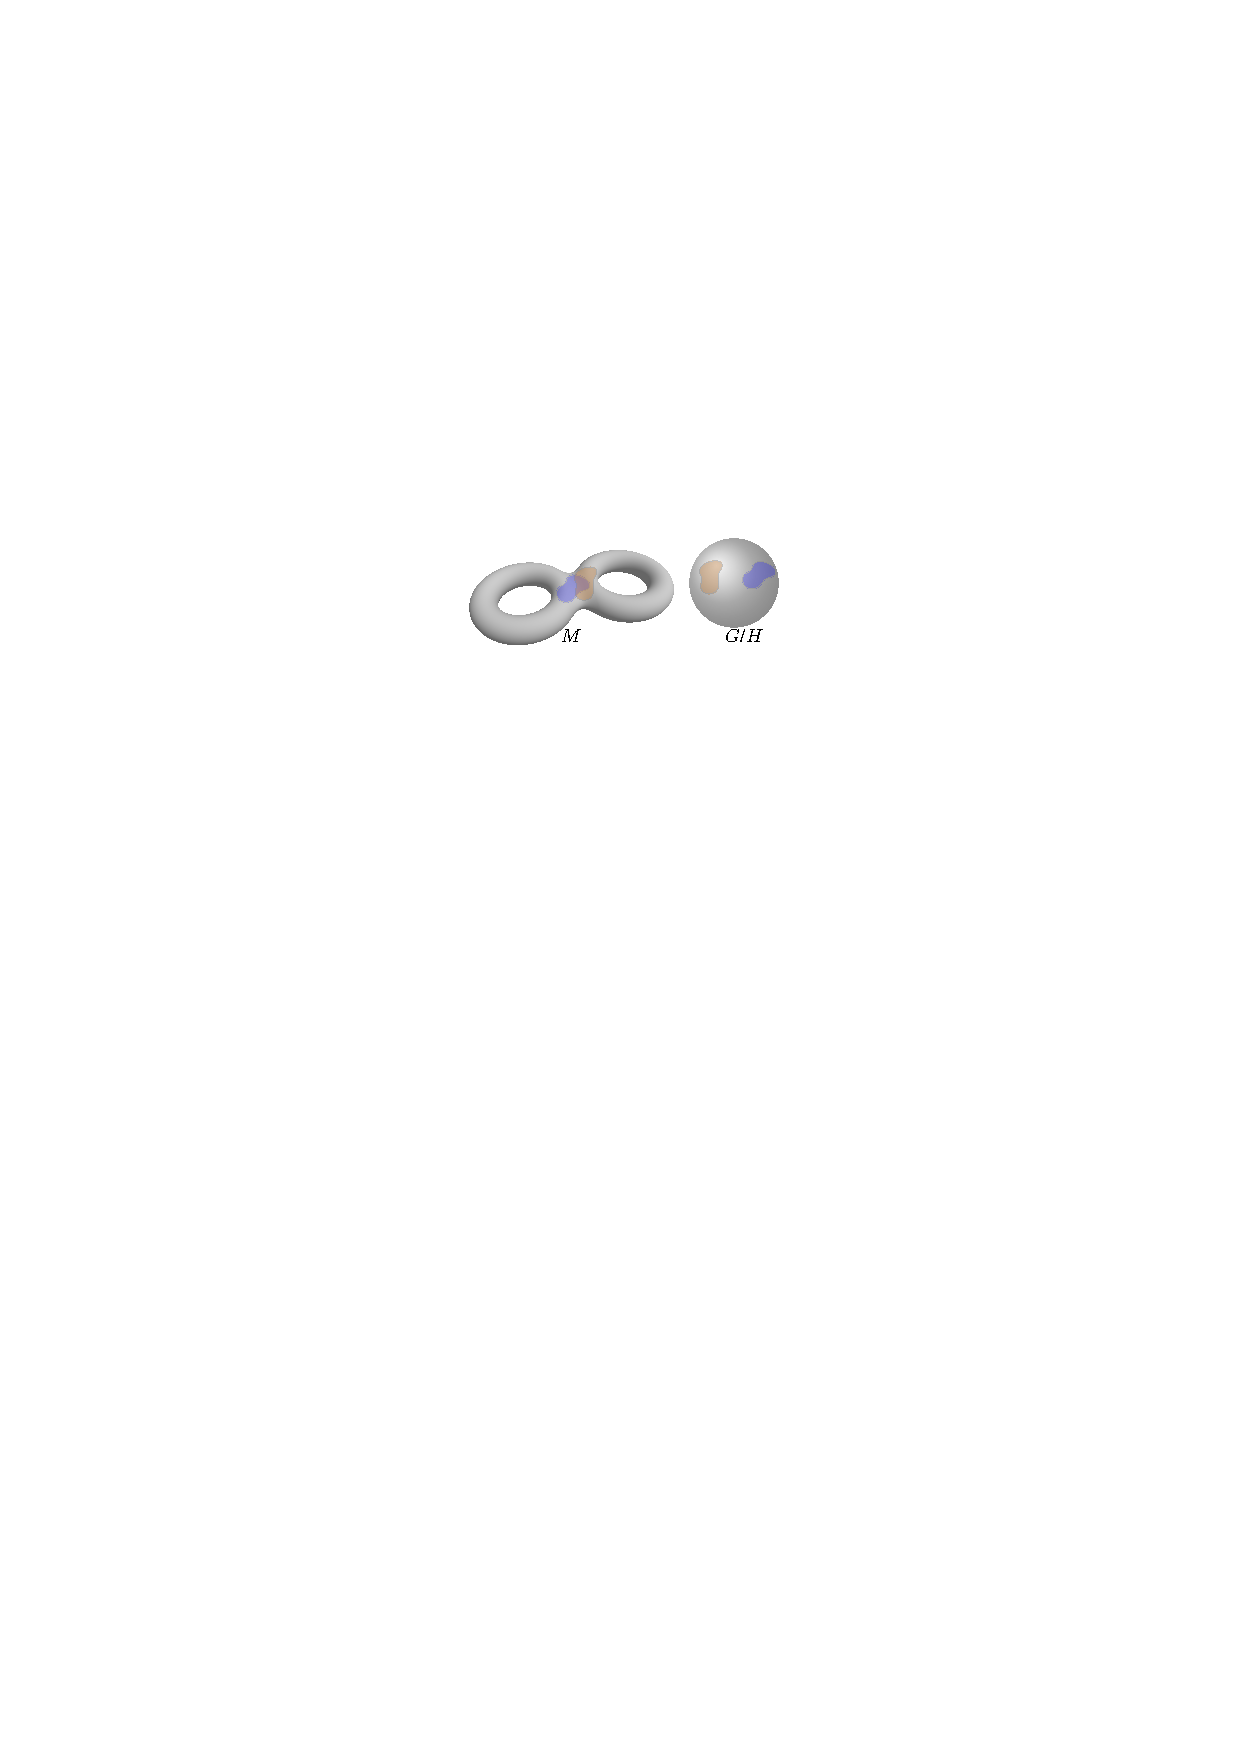
\includegraphics[scale=1.2]{figures/Klein.pdf}
    \caption{Effective locally Klein geometry.}
    \label{fig:klein}
\end{figure}

\begin{defn}[$(G,H)$-structure]\label{def GH-structure}
    A \emph{locally homogeneous structure} modeled on a homogeneous space of type $(G,H)$ is a connected manifold $M$ with a \emph{$(G,H)$-atlas} $\{(U_\alpha,\varphi_\alpha)\}_\alpha$, where $\{U_\alpha\}$ is an open covering of $M$ and $\varphi_\alpha:U_\alpha\to \wh{U}_{\alpha}\subset G\slash H$ are diffeomorphisms such that for each non-empty intersection $U_{\alpha\beta}=U_\alpha\cap U_\beta$ there exists $g_{\beta\alpha}\in G$ such that 
    \[\varphi_{\beta}=\wh{\rmL}_{g_{\beta\alpha}}\circ \varphi_\alpha\text{ on }U_{\alpha\beta}.\]
    A \emph{$(G,H)$-structure} on $M$ is a maximal $(G,H)$-atlas $\calA$. The tuple $(M,\calA)$ is called a \emph{$(G,H)$-manifold}.
\end{defn}

\begin{rem}
    We will be interested only in effective models for locally homogeneous structures, since in the ineffective case a $(G,H)$-structure is the same thing as an effective $(G/K,H/K)$-structure, where $K$ is the kernel of the Klein geometry $(G,H)$.
\end{rem}

For a deep exploration of many classical $(G,H)$-structures see the book \cite{Goldman}. We now show that this is indeed a special case of a locally Klein geometry, and that the two definitions of effective locally Klein geometries are equivalent. In light of this, the procedure of development becomes very intuitive: every local chart map is a local diffeomorphism into $G\slash H$, so by stitching them together we get a map from the universal cover to $G\slash H$. The following proposition shows that in the effective case a $(G,H)$-structure is equivalent to a locally Klein geometry.

\begin{prop}
    An effective $(G,H)$-structure on $M$ naturally induces a locally Klein geometry on $M$. Conversely, any locally Klein geometry (not necessarily with an effective model) determines a $(G,H)$-structure.
\end{prop}
\begin{proof}
    First we need to construct a principal $H$-bundle over $M$. Using the chart maps $\varphi_\alpha:U_\alpha\to G\slash H$, define the local pullback bundles  $P_\alpha\coloneqq \varphi_\alpha^\ast G$ over the $U_\alpha$. We would like to glue them into a single bundle over $M$. Since $(G,H)$ is effective, the $g_{\beta\alpha}$ in each equation $\varphi_\beta=\wh\rmL_{g_{\beta\alpha}}\circ\varphi_\alpha$ on the overlap $U_{\alpha\beta}$ is unique. This implies, in particular, that on triple overlaps $U_{\alpha\beta\gamma}$, we have $g_{\gamma\beta}g_{\beta\alpha}=g_{\gamma\alpha}$, so the cocycle condition $g_{\alpha\gamma}g_{\gamma\beta}g_{\beta\alpha}=e$ is satisfied. The left translation $\rmL_{g_{\beta\alpha}}:G\to G$ then defines the gluing diffeomorphism $\restr{P_\alpha}{U_{\alpha\beta}}\to \restr{P_\beta}{U_{\alpha\beta}}$. Even though the $g_{\beta\alpha}$ are not the transition functions of any bundle here, the fact that they satisfy the cocycle condition implies that these gluings of the local bundles $P_\alpha\to U_\alpha$ are defined consistently on all overlaps. Therefore, the $P_\alpha$ stitch together into a unique principal $H$-bundle $P\to M$. Finally, by left-invariance, the Maurer-Cartan form $\theta_G$ also pulls back to the $P_\alpha$ so that the gluing maps respect its pullbacks, and so these pullbacks stitch to a globally well-defined $1$-form $\eta\in\Omega^1(P;\frakg)$ that satisfies the definition of a locally Klein geometry.

    For the converse direction, by the Development Theorem~\ref{prop locally klein}, we get a development map $\dev:\wt M\to G\slash H$. By projection it gives rise to local diffeomorphisms $\varphi_\alpha:M\supset U_\alpha\to G\slash H$, and by the equivariance property of the developing map w.r.t.\ deck transformations, on overlaps the charts $\varphi_\alpha$ are related exactly in the way necessary to define a $(G,H)$-structure.
\end{proof}

This correspondence is, in fact, an equivalence of categories, if one restricts to isomorphisms and defines isomorphisms in the category of $(G,H)$-structures as diffeomorphisms whole local representatives in the $(G,H)$-atlases act by elements of $G$.

\begin{intu*}
    As was noted before, the discussion of locally Klein geometries is, in part, motivated by the search for an ``intrinsic'' definition of geometries on manifolds. Effective $(G,H)$-structures are a perfect example of such a definition. Manifolds themselves are defined as sets with an atlas, and we can trace most other structures on manifolds as simply imposing certain constraints on the original chart maps, and each structure compatible with the original topological structure is a choice of sub-atlas satisfying those constraints. In this way, smooth, analytic, and complex structures on a topological manifold are defined by sub-atlases with not just continuous, but smooth, resp.\ analytic and holomorphic, transition maps. Notably, fiber bundles are also defined by atlases of local trivializations, and $G$-structures on fiber bundles are defined by atlases with $G$-valued transition functions, but these definitions aren't local and therefore don't fit the same pattern. However, $(G,H)$-structures provide our first example of truly \emph{geometric} (i.e., related to actions of Lie groups) structures that can be defined \emph{without} reference to any additional fiber bundles. Instead, they are simply special kinds of sub-atlases on the original manifold $M$ itself. This concept will be later subsumed into the wider class of \emph{integrable $G$-structures}, which are exactly the $G$-structures that can be characterized by special choices of local coordinates on the base manifold. Complex and symplectic structures on manifolds are the most famous examples of integrable structures.
\end{intu*}

We will discuss locally Klein geometries (more commonly known as flat Cartan geometries) in more detail, including many important examples, in \S\ref{sec: uniformization of cartan}. To wrap up this \sect, let us look at what kind of local differential forms can be defined on $M=\varGamma\bslash G\slash H$ using the Maurer-Cartan form. The following holds for Klein and locally Klein geometries.

\begin{prop}[{{\cite[Prop.~4.7.1]{Sharpe}}}]\label{prop 4.7.1 Sharpe}
    If $\chi:\pi^{-1}(U)\to U\times H$ is a local chart for the principal bundle $G\to G\slash H$ corresponding to the local section $ s:U\to G$. Then the local representative of the Maurer-Cartan form $\theta_G$ in this chart at point $(m,h)$ is $\Ad_h^{-1}\circ  s^\ast\theta_G +\theta_H$, more strictly written as $\Ad_h^{-1}\circ  \pr_U^\ast \circ s^\ast\theta_G +\pr_H^\ast\theta_H$, and in full detail,
    \[(\chi^{-1})^\ast\theta_G(X_m,Y_h)=\Ad_h^{-1}\theta_G( s_\ast X_m)+\theta_H(Y_h),\quad X_m\in \T_mU,Y_h\in \T_h H.\label{eq prop 4.7.1 Sharpe}\]
\end{prop}
\begin{proof}
    We have $ s(m)=\chi^{-1}(m,e)$. Also let $i_h:U\to U\times H$ and $j_m:H\to U\times H$ be the inclusions of the slices $m\mapsto (m,h)$ and $h\mapsto (m,h)$, respectively. Then we have
    \[(\chi^{-1\ast}\theta_G)\circ i_{h\ast}=(\chi^{-1}\circ i_h)^\ast \theta_G=(\rmR_h s)^\ast \theta_G= s^\ast \rmR_h^\ast \theta_G= s^\ast(\Ad_h^{-1}\theta_G)=\Ad_h^{-1} s^\ast \theta_G,\]
    and on the other hand, 
    \[(\chi^{-1\ast}\theta_G)\circ j_{m\ast}=(\chi^{-1}\circ j_m)^\ast \theta_G=\rmL_{ s(m)}^\ast\restr{\theta_G}{\T_hH}=\restr{\theta_G}{\T_hH}=\theta_H.\]
\end{proof}

There is another way of interpreting this result. Let $ s_\alpha:U_\alpha\to G$ be a local gauge, that is, a local section of the principal $H$-bundle $G\to G\slash H$ over an open set $U_\alpha\subset G\slash H$. Then $ s_\alpha$ pulls back the Maurer-Cartan form $\theta_G$ to a $\frakg$-valued $1$-form $\theta_\alpha$ on $U_\alpha$: \[\theta_\alpha\coloneqq  s_\alpha^\ast\theta_G.\] 
The Maurer-Cartan equation for $\theta_G$ then yields the structure equation for $\theta_\alpha$:
\[\dd\theta_\alpha+\frac 12[\theta_\alpha,\theta_\alpha]=0.\]
Note that $\theta_\alpha$ \emph{almost} determines $ s_\alpha$ since the Fundamental Theorem~\ref{thm 6.1 Sharpe fundamental local} says that $\theta_\alpha$ determines $ s_\alpha$ up to left multiplication by a fixed element of $G$. Then, for an effective Klein geometry, if $ s$ is a section, then $g s$ is a section iff $g=e$, so in this case $ s_\alpha$ is recovered uniquely.\footnote{If $g s$ is a section, then $u=\pi(g s(u))$ and hence $g\cdot u=u$ for all $u\in U$. Thus $f^{-1}gf\in H$ for all $f\in\pi^{-1}(U)\subset G$. Thus shows that $\{f\in G\mid f^{-1}gf\in H\}$ contains an open subset of $G$. But it is also an analytic subset of $G$, so it must be equal to $G$, at least for connected $G$. Thus $g\in \bigcap_{f\in G}fHf^{-1}$, and this latter is a normal subgroup of $G$ inside $H$ and is therefore trivial.} 
For this reason we may refer to $\theta_\alpha$ as an \emph{infinitesimal gauge}. The infinitesimal gauge $\theta_\alpha$ can be roughly interpreted as assigning to each tangent vector $X_m\in \T_mM$ an infinitesimal ``motion'' $\theta_\alpha(X_m)\in \frakg$ of $M$ whose Killing vector field at $m$ coincides with $X_m$.

By differentiating the transformation rule $ s_\beta(m)= s_\alpha(m)h_{\alpha\beta}(m)$ (cf.\ \eqref{eq transf rule for sections}) we get
\[ s_\beta^{\ast}\theta_G=\Ad_{h_{\alpha\beta}}^{-1} s_\alpha^\ast\theta_G+h_{\alpha\beta}^\ast\theta_H,\]
that is
\[\boxed{\theta_\beta=\Ad_{h_{\alpha\beta}}^{-1}\theta_\alpha+h_{\alpha\beta}^\ast\theta_H.}\]
This transformation, equivalent to \eqref{eq prop 4.7.1 Sharpe}, is called an \emph{passive local gauge transformation}, and the two infinitesimal gauges are called \emph{gauge equivalent}.

Since in the effective case the $\theta_\alpha$ let us recover the local sections $s_\alpha$ uniquely, one can give an alternative definition of effective locally Klein geometries in terms of a collection of local $1$-forms on $M$ satisfying the structure equation and the above compatibility rule (gauge equivalence). Up to isomorphism, this allows one to reconstruct the principal bundle of the geometry and the global form $\eta$. Completeness is a little more subtle, so we shall delay this approach to locally Klein geometry until our discussion of flat Cartan geometries in \S\ref{sec: uniformization of cartan}.

\begin{rem}
    We have the non-canonical isomorphism at every $m\in U_\alpha$
    \[\underline{\theta}_\alpha:\T_mU_\alpha\overset{\theta_\alpha}{\longrightarrow}\frakg\overset{\mod\frakh}{\longrightarrow} \frakg\slash\frakh.\]
    Indeed, one of the defining properties of $\theta_G$ is that its value belongs to $\frakh$ \emph{only} for \emph{vertical} directions on the bundle $G\to G\slash H$, so its pullback $\theta_\alpha$ by a section can never attain values in $\frakh$. This establishes that the quotient $\frakg\slash\frakh$ naturally plays the role of the model tangent space of the effective homogeneous space $G\slash H$. In \S\ref{sec: homogeneous bundles} we will see that this is true for non-effective spaces as well, but in the effective case $\underline\theta_\alpha$ provide non-natural local trivializations of the tangent bundles. We will return to the tangent bundle of a homogeneous space in \S\ref{sec: homogeneous bundles}.
\end{rem}

% \begin{intu*}
%     An effective locally Klein geometry is completely characterized by the collection of local $1$-forms $\{\theta_\alpha\}$ on $M$. By picking an arbitrary basis in the Lie algebra, $\frakg$, we can identify $\theta_\alpha$ with a collection of $d=\dim G$ scalar local $1$-forms on $M$, called an \emph{extended moving coframe} (since $d\geq \dim M$). By retracing the steps of the above derivations, one can recover the local charts identifying subsets of $M$ and $G\slash H$. If $M=G\slash H$, then any local diffeomorphism of $M$ that preserves the form $\theta_\alpha$ is an automorphism of the Klein geometry, and hence coincides with a group action $\wh \rmL_g$. Thus, the preservation of moving coframes uniquely determines the principal group of motions defining the Klein geometry. Describing group action by a collection of differential $1$-forms an extremely powerful computational gadget that is at the core of Cartan's geometric methods. We will learn to describe completely general Lie group actions via moving coframes in \Chap~\ref{ch equivalence problems}.
% \end{intu*}


% \begin{defn}[Effective locally Klein geometry III]
%     An effective locally Klein geometry \emph{modeled on} an effective Klein geometry $(G,H)$ is a connected manifold $M$ with a collection $\{(U_\alpha,\theta_\alpha)\}_\alpha$, where $\{U_\alpha\}$  is an open covering of $M$ and each $\theta_\alpha\in \Omega^1(U_\alpha;\frakg)$ is a $\frakg$-valued local $1$-form that satisfies the structure equation 
%     \[\dd\theta_\alpha+\frac12 [\theta_\alpha,\theta_\alpha]=0,\]
%     and such that on every intersection $U_{\alpha\beta}$ there exists a smooth function $h_{\alpha\beta}:U_{\alpha\beta}\to G$ such that 
%     \[\theta_\beta=\Ad_{h_{\alpha\beta}}^{-1}\theta_\alpha+{h_{\alpha\beta}}^\ast\theta_H.\]
% \end{defn}




% \begin{example}[Meteor tracking]
%     Suppose we live in a small open set $U\subset M=G\slash H$ and a meteor flashes through $U$. We wish to describe its motion. We formalize the meteor as a point set $X$, and a \emph{configuration} of the meteor is a map $X_0:X\to M$. This is the origin for Cartan's idea of a ``moving frame''.\index{Moving frames}
    
%     We assume the meteor is \emph{rigid} and \emph{sufficiently complicated}. By the term rigid in the given geometry, we mean that for any two of its positions, where it has the configurations $X_0$ and $X_1$ say, there is an element of $G$ carrying $X_0$ to $X_1$. By sufficiently complicated we mean that the subgroup of $G$ that fixes the body pointwise (its stabilizer) is the identity.  It follows that if $X(t)$ is the configuration of its points at time $t$, then there is a unique path $g(t)\in G$ such that $X(t)=g(t)X(0)$. One way to describe the motion would be to specify the path $g(t)$ itself. However, it is more useful, and closer to what is actually observed, to describe the motion differently. We first describe the motion of one of its points $q\in X(0)$, which we take to be $eH$, by a path $q(t)=g(t)H$ on $U$, and then describe the motion of the rest of the body as turning about this one point as it moves along. For this we will need the concept of a gauge.

%     Let us assume that $U$ is small enough to admit a local section $s:U\to G$. Any two such sections $s,s'$ are related by a map $h:U\to H$ by $s'(u)=s(u)h(u)$. A ``choice of gauge'' is a choice of such a local section, and $h(u)$ is called a gauge transformation. A choice of gauge can be regarded as a choice of motions, varying smoothly with $u$, which maps the base point to $u$. The value of a gauge at any point may be called a \emph{frame} at that point and the gauge itself may be called a \emph{moving frame}. From this point of view the principal bundle $G\to G\slash H$ is a bundle of frames.

%     Since both $s(q(t))$ and $g(t)$ lie over $q(t)$, they must differ by an element $k(t)\in H$. Thus, in the presence of a gauge, the motion can be described by giving $q(t)$ and $(k(t)$. The latter describes the way the meteor turns about the point $q(t)$. Crucially, there is no intrinsic geometric meaning attached to the choice of gauge $s$, or the function $k(t)$ alone. Together, however, they complete the description of the motion.
% \end{example}


\begin{example}
    Recall the \emph{hyperbolic upper half-plane} $\bbC^+=\SL_2(\bbR)\slash \SO_2$ from Example~\ref{ex siegel upper half-space}. The Uniformization Theorem of Riemann Surfaces states that any closed (compact with no boundary) orientable \emph{simply connected} surface with its conformal/projective/complex structures is isomorphic to one of three: the Riemann sphere $\CP^1$, the plane $\bbC$, or the upper half-plane $\bbC^+$.

    In the case of $\CP^1$, it is not the covering space of anything else, so every genus $0$ surface is isomorphic to $\CP^1$. In the case of $\bbC$, every properly discontinuous action is determined by a lattice $\varLambda\subset \bbC$, so the quotient $\bbC\slash\varLambda$ has genus $1$, and thus every Riemann surface of genus $1$ is isomorphic to such a quotient. Finally, any oriented surface $\varSigma_g$ of genus $g>1$ is isomorphic to $\varGamma\bslash \bbC^+$ for some choice of discrete subgroup $\varGamma<\SL_2(\bbR)$. Let $\varGamma_g$ be such a subgroup. Then $\varSigma_g\cong \varGamma_g\bslash \bbC^+$ is a locally Klein geometry.
\end{example}

\begin{rem}
    The Uniformization Theorem of Riemann Surfaces itself can be proven by reduction to the Uniformization Theorem of flat Cartan geometries, but the hard part is in fully demonstrating that every Riemann surface carries a \emph{complete} Cartan connection. The standard way of doing this is by constructing a complete Riemannian metric on the surface; these metrics are chosen so as to have constant Gauss curvature, which makes them flat Cartan geometries. One could also approach this by constructing a \emph{holomorphic projective connection} (i.e., a holomorphic Cartan connection of type $(\PSL_2(\bbC),\U_1)$ with model space $\CP_1$) on every Riemann surface, which will be automatically flat because surfaces are $1$-dimensional over complex numbers. The projective connection then needs to be appropriately deformed so that the development map to $\CP^1$ is biholomorphic. All of these approaches and their history can be found in the famous book \cite{Gervais} (Henri Paul de Saint-Gervais is a pen name for a collective of mathematicians, referencing Henri Poincar\'e, Paul Koebe, and the French town where the collective first met).
\end{rem}

\begin{example}[Moduli spaces of algebraic curves]
    An \emph{elliptic curve} is a Riemann surface $\varSigma$ of genus $1$. Per the preceding example, $\varSigma\cong \bbC\slash\varLambda$ for some lattice $\varLambda\subset\bbC$, hence $\varSigma$ is a homogeneous space. Any biholomorphism between elliptic curves arises from a complex affine linear map $\bbC\to\bbC$ matching lattices. We can always arrange by isomorphism that $\varLambda$ is generated by $1,\tau$ for some $\tau\in \bbC^+$. But then $\tau$ is only determined up to \glspl{flt} of $\bbC^+$ with integer coefficients (so that $1$ is a fixed point). Hence, the ``coarse moduli space'' of elliptic curves is a complete Klein manifold $\varGamma\bslash \bbC^+$, where $\varGamma\cong \SL_2(\bbZ)$ is the set of \glspl{flt} with integer coefficients. Similarly, the coarse moduli space of compact Riemann surfaces of genus $g$ is a complete Klein manifold $\Sp_{2g}(\bbZ) \bslash \calH_g$ where $\calH_g$ is the complex hyperbolic space of real dimension $g(g+1)$ (cf.\ Example~\ref{ex siegel upper half-space}).
\end{example}


\begin{example}[Affine elliptic curves]
    Every elliptic curve $E=\bbC\slash\varLambda$ has a complex affine structure, i.e., $G=\bbC^\times\ltimes\bbC$ and $H=\bbC^\times$. The developing map is the identity $\dev^0=\id_\bbC$ and the holonomy homomorphism is 
    \[\hol^0:\varLambda\to G,\quad \lambda\mapsto (1,\lambda).\]
    There are other affine structures on $E$. For every $c\in \bbC^\times$, we can produce an affine structure on $E$ via the developing map $\dev^c:\bbC\to \bbC^\times,$ $z\mapsto \rme^{cz}$, with holonomy morphism 
    \[\hol^c:\varLambda\to G,\quad \lambda\mapsto (\rme^{c\lambda},0).\]
    Since the developing map of an affine structure is unique up to affine transformations, we could just as well use the map $z\mapsto c^{-1}(\rme^{cz}-1)$, which lets us think of $\dev=\id_\bbC$ as the limiting case $c\to 0$.  To forget the choice of affine coordinate $z$, we can identify the moduli space of affine structures on an elliptic curve $E$ with the space of holomorphic $1$-forms on $E$: each $1$-form is expressed in terms of an affine chart as $c\dd z$. The developing map $\dev^c$ is a map to the \emph{linear} geometry on $\bbC\setminus\{0\}$, i.e., $(G',H')=(\bbC^\times,\{e\})$.  The holomorphic $1$-form $\dd\zeta/\zeta$ on $\bbC\setminus\{0\}$, with the standard coordinate $\zeta$, is $G'$-invariant (in fact, it is the Maurer-Cartan form of $\bbC^\times$), and pulls back to $c\dd z$ on $\bbC$. Hence, we identify the isomorphism class of the affine structure with this induced holomorphic $1$-form, and take the zero $1$-form as the limit $c\to 0$.  It is known that every holomorphic affine structure on an elliptic curve arises uniquely this way. The automorphism group of the affine structure with $c=0$, the one with linear developing map, is the biholomorphism group of the elliptic curve (which is a semidirect product of the translation group $\bbC$ with a finite group of at most $24$ elements). The automorphism group of any of the affine structures with $c\neq 0$ is only the group $\bbC$ of translations.
\end{example}

\begin{example}[Projective structures on Riemann surfaces]\index{Projective structure}\label{ex projective structure}
    A \emph{Riemann surface}\index{Riemann surface}, also called a \emph{complex curve}, is a connected $1$-dimensional complex manifold $\varSigma$, i.e., its atlas consists of $\bbC$-valued maps with complex analytic, or holomorphic, transition maps (in the $1$-dimensional case holomorphic maps are also called conformal, although the equivalence between these terms is nontrivial, cf.\ Remark~\ref{rem holomorphic functions}). Thus, the inverses of the transition maps are also complex analytic, so that the transition maps are \emph{biholomorphic}.\index{Biholomorphism} Now, a \emph{projective structure} $\calP$ on $\varSigma$ is a $(\PSL_2(\bbC),\U_1)$-structure in the sense of Definition\ \ref{def GH-structure}. In particular, the chart maps are \emph{meromorphic} biholomorphisms, i.e., they take values in $\CP^1$ instead of just $\bbC$ (so they are allowed to have simple poles). The pair $(\varSigma,\calP)$ is called a \emph{complex projective surface}.
    
    Every Riemann surface admits many non-equivalent projective structures, but the Uniformization Theorem (stating that there is a unique, up to a \gls{flt}, biholomorphism between the universal cover of $\varSigma$ and one of three standard subsets of $\CP^1$) implies the existence of a \emph{canonical projective structure}.
    Moreover, every affine structure induces a projective structure via the obvious inclusion $\bbC\cong \CP^1\setminus \{\infty\}\to \CP^1$. Among the various affine structures on elliptic curves given above, each induces a distinct projective structure, except for pairs $\{c,-c\}$, which are clearly related by a \gls{flt}, $\rme^{-cz}=\frac{1}{\rme^{cz}}$. It turns out that these are all of the projective structures on $E$: we can identify the moduli space of projective structure on any elliptic curve with the space of quadratic differentials $c^2\dd z^{\otimes 2}$, as we will see. For $c\neq 0$, the developing map is $z\mapsto \rme^{cz}\in \CP^1$ and the holonomy homomorphism is 
    \[\hol^c:\lambda \mapsto \begin{bmatrix}
        \rme^{c\lambda/2} & 0\\
        0 & \rme^{-c\lambda/2}
    \end{bmatrix}\in G.\]
    For $c=0$, the developing map is the inclusion map $\bbC\to \CP^1$ and the holonomy morphism is 
    \[\hol^0:\lambda\to \begin{bmatrix}
        1 & \lambda \\ 0 & 1
    \end{bmatrix}\in G.\]
    The automorphism group of the projective structure at $c=0$ is still the biholomorphism group of the curve. At $c\neq 0$, the automorphism group is $\bbZ_2\ltimes\bbC$, where $\bbZ_2$ acts on $\bbC\slash\varLambda$ by $z\mapsto -z$ and $\bbC$ acts by translations.

    Clearly, $\CP^1$ has an obvious projective structure, being the model geometry. The developing map and the holonomy homomorphism are trivial and the biholomorphism group is $G=\PSL_2(\bbC)$.
\end{example}

\begin{example}
    In many cases of interest, namely when the principal bundle can be identified with some $H$-structure, a $(G,H)$-structure on $M$ is equivalent to the specification of a $G$-invariant geometric object on $G\slash H$. The most prominent example is a locally homogeneous Riemannian metric. For example, if $X$ is a simply connected Riemannian manifold of constant curvature $K$ and $G$ is its group of isometries with stabilizer $H$, then locally modeling $M$ on $X\cong G\slash H$ is equivalent to giving $M$ a metric of constant curvature $K$. In particular, Riemannian surfaces of constant curvature can all be given locally homogeneous structures of either the round sphere (if $K>0$), the plane (if $K=0$), or the hyperbolic half-plane ($K<0$). 
    % If the surface is complete (as a locally homogeneous structure, or, equivalently, geodesically complete), the developing map identifies one of these three models with the universal cover of the surface. This is another version of the Uniformization Theorem of Riemann Surfaces.
\end{example}

For more examples of locally Klein geometries, see \S\ref{sec: uniformization of cartan}.






\section{Morphisms}\label{sec: morphisms of klein geom}

In this \sect\ we discuss changing the models of $(G,H)$-structures via morphisms. We use the term ``$(G,H)$-structure'' loosely to refer to locally Klein geometries of type $(G,H)$.

\begin{defn}[Morphism of Klein geometries]
    If $(G,H)$ and $(G',H')$ are two Klein geometries, then a morphism between them \emph{modeled on} a Lie group homomorphism $\lambda:G\to G'$ such that $\lambda(H)\subset H'$ is a right $\lambda$-equivariant smooth map $\vartheta:G\to G'$ (i.e., $\vartheta(gh)=\vartheta(g)\lambda(h)$ for $g,h\in G$). Equivalently, it is a morphism $\vartheta :G\to G'$ of the principal bundles $G\to G\slash H$ and $G'\to G'\slash H'$ which is right $\lambda$-equivariant, or whose base map $\underline{\vartheta}:G\slash H\to G'\slash H'$ is $G$-equivariant: $\underline{\vartheta}([g])=\wh{\rmL}_{\vartheta(g)}([e])$.
\end{defn}

Note that any right $\lambda$-equivariant map $\vartheta:G\to G'$ differs from $\lambda$ only by a left translation: $\vartheta=\rmL_{g'}\circ\lambda$ for some $g'\in G'$ (cf.\ Proposition~\ref{prop lambda-equiv maps}). Since left translations are automorphisms of Klein geometries, in practice it suffices to consider morphisms which are homomorphisms, i.e., $\vartheta=\lambda$. We will proceed under this assumption and write such morphisms as $\lambda:(G,H)\to (G',H')$.

\begin{example}
    The double cover $\bbS^n\to \RP^n$ can be realized as a morphism of two Klein geometries $(G,H)\to (G',H')$, where $G\cong\SL_{n+1}(\bbR)\times\bbZ_2$ is the subgroup of $\GL_{n+1}(\bbR)$ consisting of matrices with determinant $\pm 1$,  and $G'=\SL_{n+1}(\bbR)$ is the identity component of $G$ (note that $H\cong H'$). Then $\bbS^n\to \RP^n$ is $\lambda$-equivariant with $\lambda(g)=g/\det g$.
\end{example}

Given a manifold $M$ with a $(G,H)$-structure (with its principal $H$-bundle $P\to M$) and a morphism $\lambda:(G,H)\to (G',H')$ of models, we can induce a $(G',H')$-structure by composing the charts with the $G$-equivariant base map $\underline{\lambda}$. This also gives the new $H'$-bundle $P'\to M$.

Conversely, given a $(G',H')$-structure $(P'\to M,\eta)$, it is interesting to ask whether it is induced from a $(G,H)$-structure $(P\to M,\eta)$. Factoring $(G,H)\to (G',H')$ into two maps 
\[(G,H)\to (\lambda(G),\lambda(H))\to (G',H'),\]
we are able to split the question into two separate problems, where the morphism is surjective in one and injective in the other.

First consider surjective morphisms. First, to be able to reconstruct a $\frakg$-valued form from a $\frakg'$-valued one, we clearly need $\lambda:G\to G'$ to be a covering homomorphism. Then $H\to \lambda(H)$ is also a covering map. If the bundle $P'\to M$ is associated to some smooth principal $H$-bundle $P\to M$ via (the restriction of) a homomorphism $\lambda:G\to G'$ and if $\lambda_{\ast e}:\frakg\to \frakg'$ is an isomorphism, we just let 
\[\eta\coloneqq \lambda^{-1}_{\ast e}\circ \iota_e^\ast \eta',\] where $\iota_e:P\to P'$, $p\mapsto [(p,e)]$, is the canonical covering map. This induces a $(G,H)$-structure on $P\to M$. 

\begin{example}
    \begin{enumerate}
        \item Consider the trivial double cover $(\tuple{\Aff_n(\bbR),\GL_n(\bbR)})\to(\tuple{\Aff_n^+(\bbR),\GL_n^+(\bbR)})$. Thus, any oriented affine manifold can be turned into a regular affine manifold (e.g., by adding reflected chart maps to the atlas).
        \item Consider the nontrivial double cover $(\Spin_n\ltimes\bbR^n,\Spin_n)\to (\SE_n,\SO_n)$. Thus, assuming we are given a corresponding covering bundle morphism $P\to P'$, then we can reconstruct the affine spin structure from the affine Riemannian structure. The assumption of the existence of a covering spin bundle here is crucial because not every Riemannian structure admits one, or may admit multiple.
        \item If $M=\bbS^1$, then, by picking an arbitrary locally Klein geometry $\eta$ and developing it, all bundles over $M$ are quotients of the form $P=(\bbR\times H)\slash \sim$, where $(x,h)\sim (x+1,h_0h)$ with $h_0$ (the generator of monodromy) determined up to conjugacy. So every element of $H'$ is conjugate to an element of the image $\lambda(H)< H'$ iff all $H'$-bundles arise from $H$-bundles.
        \item If $M$ is contractible, then every $(G',H')$-structure on it lifts to a $(G,H)$-structure since all bundles over $M$ are trivial.
        \item If $M=\bbS^n$, it has a covering by two open sets whose intersection deformation retracts to the equator. So if the induced homomorphism of homotopy groups $\pi_{n-1}(H)\to \pi_{n-1}(H')$ is surjective, we can lift every $H'$-bundle on $\bbS^n$ to an $H$-bundle.
    \end{enumerate}
\end{example}


\begin{example}[Monopole bundles]\label{ex monopole bundles}\index{Monopole!bundles}\index{Hopf fibration}
    Consider the Hopf bundle $\bbS^3\to \bbS^2$ defined as a $\U_1$-principal bundle, or as a Klein geometry of type $(\SU_2,\U_1)$, cf.\ Example~\ref{ex Hopf principal bundle}, where the $\U_1$ subgroup multiplies by diagonal matrices of the form $\diag(\rme^{\i \varphi},\rme^{-\i\varphi})$ from the right. Let $q\in\bbZ$ and $\lambda:\U_1\to \U_1$ be the homomorphism $\lambda(z)=z^q$ with kernel $\varGamma=\bbZ_q\subset \U_1$. Since the structure group is Abelian, the left-invariant Maurer-Cartan form on $\SU_2$ is also right-invariant, and hence we can take a \emph{right} quotient by this discrete group and still obtain a locally Klein geometry whose fibers ``twist $q$ times faster'' than in the Hopf bundle. The space $\bbS^3\slash\Gamma$ is the lens space $L(q;1)$ (cf.\ Example~\ref{example Lens spaces}). We get the principal $\U_1$-bundle
    \[L(q;1)\to L(q;1)\slash \U_1=\bbS^2\]
    (since the induced action of $\U_1$ on $L(q;1)$ is trivial) and a $\lambda$-equivariant covering morphism of $\U_1$-bundles $\vartheta:\bbS^3\to L(q;1)$, which looks similar to $\lambda$ on every fiber.
    
    Since the transition functions in the new bundle can be obtained by composition with $\lambda$, in the standard atlas consisting of two hemispheres (Example~\ref{ex hopf bundle atlas}), the transition function of this new bundle is $\tau_{-+}(z)=z^{-q}$, i.e., this is exactly the $\U_1$-bundle with Chern number $-q$ from Example~\ref{ex circle bundles over S2}. This proves that the lens space is simultaneously $\bbS^3\slash \bbZ_q$ and the gluing of two solid tori, thus solving Exercise~\ref{xca two definitions of lens spaces}. As principal $\U_1$-bundles, these bundles are known as \emph{monopole bundles}. The Maurer-Cartan form of $\SU_2$ induces an $\fraksu_2$-valued $1$-form $\eta$ on $L(q;1)$ which we will later interpret as the Cartan connection of a magnetic monopole of charge $q$, see Example~\ref{ex connection on monopole bundles}.

    We thus have the surjective vertical morphism of principal bundles $\vartheta:\bbS^3\to L(q;1)$ given by the quotient by the $\bbZ_q$-action and the group homomorphism $\lambda:\U_1\to \U_1$ given by the $q$-fold covering of the circle $z\mapsto z^q$. Note that these bundles are also defined for $q$ negative as the duals (inverse transition functions), or via the inverse $\U_1$-action on $\bbS^3$.
\end{example}


In the injective case, not every structure on $P'$ is induced from one on $P$, and we will have to learn about general Cartan connections before we identify the criterion for this via holonomy in Theorem~\ref{thm 16.30 McKay}. Nevertheless, let us return to the problem of what structure a Klein geometry (i.e., its principal bundle and Maurer-Cartan form) can induce under morphisms. We will describe the new principal bundle $P'$ and its associated form $\eta'$ in a language more suited to our ultimate study of Cartan geometries. The following details may be safely skipped on first reading.

\begin{lem}[{{\cite[Lem.~16.2]{McKayCartan}}}]\label{lem 13.2 McKay}
    Let $\lambda:(G,H)\to (G',H')$ be a morphism of Klein geometries (or homogeneous spaces). Denote $M\coloneqq G\slash H$ and $M'\coloneqq G'\slash H'$. Also denote $H''\coloneqq \lambda^{-1}(H')< G$ and $M''\coloneqq \underline{\lambda}(M)\subset M'$ (note that $H<H''$). Then $\underline{\lambda}\circ\pi:G\to M''$ is a principal $H''$-bundle and is associated to the $H'$-bundle $\restr{G'}{M''}\to M''$. 
    
    In more detail, define $\psi:G\times H'\to G'$ by $\psi(g,h')=\lambda(g)h'$. Then, at any point $(g,h')\in G\times H'$, 
    \[\psi^\ast\theta_{G'}=\theta_{H'}+\Ad_{h'}^{-1}\circ\lambda_{\ast e}\circ \theta_G.\] 
    The map $\psi$ is a surjective $H''$-bundle map to $\restr{G'}{M''}$ under the right $H''$-action $(g,h')\cdot h\coloneqq (gh,\lambda(h)^{-1}h')$, $H'$-equivariant under the right $H'$-action $(g,h')\cdot k'\coloneqq (g,h'k')$, and $G$-equivariant under the left $G$-action $a(g,h')\coloneqq (ag,h')$. Quotienting by that right $H''$-action gives an $H'$-bundle isomorphism 
    \[\begin{tikzcd}
        G\times^{H''}H'\arrow[rr,"\cong"]\arrow[dr] & & \restr{G'}{M''}\arrow[dl]\\
        & M''. &
    \end{tikzcd}\]
\end{lem}
\begin{proof}
    The map $\psi$ is clearly invariant and equivariant in the three stated ways, therefore it descends as stated to a map $G\times^{H''} H'\to G'$. Its image is clearly the pullback $\restr{G'}{M''}$ of $G'\to M'$ to $M''\subset M'$. By $G$-equivariance, $M''$ is a $G$-orbit in $M'$, so a smooth manifold. Two elements $(g,h)$, $(\wt g,\wt h)\in G\times H'$ map to the same point $g'\in G'$ iff $\lambda(g)h=\lambda(\wt g)\wt h$, i.e., $\lambda(g^{-1}\wt g)=h\wt{h}^{-1}$, so $\wt{g}=gk\in \lambda^{-1}(H')=H''$ and $\lambda(k)=h\wt{h}^{-1}$ so $\wt{h}=\lambda(k)^{-1}h$. So the map $\psi$ descends to an injection $G\times^{H''}H'\hookrightarrow G'$. 

    The subgroup $H''=\lambda^{-1}(H')$ is a closed Lie subgroup since $H'\emb G'$ is closed. Hence, it acts on $G$ freely and properly, hence acts on $G\times H'$ freely and properly, so the quotient is a smooth manifold and $G\times H'\to G\times^{H''}H'$ is a smooth principal $H''$-bundle, and the map to $G'$ is smooth. The left $G$-action and right $H'$-action on $G\times H'$ are smooth, and invariant under the right $H''$-action, so descend to smooth $\psi$-equivariant actions on the quotient.

    Thus, $G\times^{H''}H'\to \restr{G'}{M''}$ is an equivariant bijection of homogeneous spaces of $G\times H'$, hence a diffeomorphism, and a bundle isomorphism over $M'$ by equivariance. The formula relating the Maurer-Cartan forms is just the differential-geometric version of the matrix identity 
    \[(gh')^{-1}\dd (gh')=(h')^{-1}g^{-1}(g\dd h'+\dd g \cdot h')=(h')^{-1}\dd h'+(h')^{-1}(g^{-1}\dd g)h'.\]
\end{proof}

In other words, a morphism of Klein geometries induces a principal $H''$-bundle with a special $\frakg'$-valued differential form. The dimension of $\frakg'$ doesn't even necessarily match the dimension of the bundle, but it does if $\underline\lambda$ is a local diffeomorphism, e.g., a covering map. Note that this situation, threated in the following corollary, is more general than the examples given earlier, since $\lambda$ itself need not be a local diffeomorphism.

\begin{cor}
    In the setting of the preceding lemma, let $\underline{\lambda}:G\slash H\to G'\slash H'$ be a local diffeomorphism. Let $(P\to M,\eta)$ be a locally Klein geometry of type $(G,H)$. Then the  geometry of type $(G',H')$ associated to this one via the morphism $\lambda$ has bundle $P'=P\times^{H''}H'$ and its form $\eta'$ pulls back to $P\times H'$ to become (omitting obvious pullbacks)
    \[\eta'=\theta_{H'}+\Ad_{h'}^{-1}\circ\lambda_{\ast e}\circ\eta.\]
\end{cor}
\begin{proof}
    From the preceding lemma, this holds on each of the $H$-invariant open sets in $P$ which are identified by the local bundle charts with $H$-invariant open subsets of $G$. By $G$-equivariance, this description glues together under the transition maps to cover all of $P$ and $P'$.
\end{proof}

The resulting form $\eta'$ on the $H'$-bundle $P'$ satisfies all properties of a locally Klein geometry \emph{except} for the structure equation. Hence, this procedure takes us outside of the category of locally Klein geometries and into the category of general Cartan geometries. We will need this construction when we study \emph{mutations} of Cartan geometries. The key insight will be that the above procedure is reversible, and so one can freely move between certain flat and curved geometries.






\section{Homogeneous bundles}\label{sec: homogeneous bundles}


We now consider the tangent bundle of a Klein geometry. Tangent spaces of a Lie group $G$ are canonically identified with the Lie algebra $\frakg$ (using the Maurer-Cartan form), so it is natural to expect that the tangent spaces of a homogeneous space $G\slash H$ should be identified with the quotient $\frakg\slash\frakh$. However, as we will now show, this identification is not canonical. On the principal bundle $G\to G\slash H$, local trivializations induce local diffeomorphisms of the form $\T(\pi^{-1}(U))\cong \T(U\times H)\to \T U\times \T H$, where $U\subset G\slash H$. Local trivializations of $\T (\pi^{-1}(U))$ and $\T H$ are given by the Maurer-Cartan forms $\theta_G$ and $\theta_H$, respectively, and on vertical directions $\theta_H$ coincides with the representative of $\theta_G$. In other words, the restriction of $\theta_G$ to vertical directions produces a \emph{canonical} global trivialization of the \emph{vertical} bundle $\calV G\to G\slash H$. At a particular point $g\in G$, we can quotient out the vertical directions, and this corresponds to quotienting $\frakg$ by $\frakh$. Thus, choosing a point $g\in G$ over $m=[g]\in G\slash H$, we have the commutative diagram
\[
\begin{tikzcd}
    0\arrow[r]&\calV_g G\arrow[r]\arrow[d,"\theta_H","\cong"'] & \T_g G\arrow[r,"\mod \calV_g G"]\arrow[d,"\theta_G","\cong"'] & \T_m(G\slash H)\arrow[d,dashed,"\chi_g","\cong"'] \arrow[r] & 0\\
    0\arrow[r]&\frakh\arrow[r,hookrightarrow]&\frakg \arrow[r,"\mod \frakh"] & \frakg\slash \frakh\arrow[r]  & 0
\end{tikzcd}
\]
with exact rows. The linear isomorphism $\chi_g$ is the unique map making the diagram commute, namely, 
\[\chi_g(X)=\theta_G(\wt X)+\frakh\quad \in\frakg\slash\frakh,\]
where $X\in\T_m(G\slash H)$ and $\wt X\in\T_g G$ is an arbitrary lifting of $X$, i.e., $\pi_\ast \wt X=X$.
Thus, we can identify the tangent space of $G\slash H$ at $m$ with $\frakg\slash\frakh$, but the identification $\chi_g$ depends on the choice of $g\in G$ over $m$. In fact, the relation $\rmR_h^\ast \theta_G=\Ad_h^{-1}\theta_G$ implies that $\chi_{gh}=\underline{\Ad}_h^{-1}\circ \chi_g$, where $\underline{\Ad}_h$ is the induced $H$-action on $\frakg\slash \frakh$ (it will be properly defined below). It follows that the identification of $\T_m(G\slash H)$ with $\frakg\slash \frakh$ is not natural, and instead is determined only up to the action of $H$ on $\frakg\slash\frakh$. This accounts for the frequent occurrence of the adjoint action in the sequel.

\begin{prop}[{{\cite[Prop.~4.5.1]{Sharpe}}}]\label{prop 4.5.1 Sharpe}
    $\T(G\slash H)\cong G\times^H (\frakg\slash\frakh)$ as \glspl{vb} over $G\slash H$.
\end{prop}
\begin{proof}
    Define a map $\varphi:G\times \frakg\to \T(G\slash H)$ by $\varphi(g, A)=(\pi(g),\pi_\ast \circ \rmL_{g\ast}A)$, where $\pi:G\to G\slash H$ is the canonical projection. Clearly $\varphi$ is smooth, surjective, and fiberwise linear. Moreover, for $A\in \T_eH$, $\rmL_{g\ast}A\in \calV_g G\in\ker\pi_\ast$. Thus, $\varphi(g, A)=(g,0)$. On the other hand,
    \begin{multline}
        \varphi(gh,\Ad_h^{-1}A)=(\pi(gh),\pi_\ast \rmL_{gh\ast}\Ad_h^{-1}A)=(\pi(g),\pi_\ast(\rmL_{gh\ast}\rmL_{h\ast}^{-1} \rmR_{h\ast}A))=\\
        =(\pi(g),\rmL_{g\ast }\pi_\ast (\rmR_{h\ast}A))=(\pi(g),\rmL_{g\ast}(\pi \rmR_h)_\ast A)
        =(\pi(g),\rmL_{g\ast}(\pi_\ast A))=\varphi(g,A).
    \end{multline}
    Thus $\varphi$ induces a smooth quotient map $\psi:G\times^H (\frakg\slash\frakh)\to \T(G\slash H)$. Moreover, this map is injective since $\varphi(g,A)=\varphi(g',A')$ implies $g'=gh$ for some $h\in H$ and $\pi_\ast \rmL_{gh\ast}A'=\pi_\ast \rmL_{g\ast}A$. The latter means that $\pi_\ast \rmL_{h\ast}A'=\pi_\ast A$ and hence that $A'-\Ad_h^{-1}A\in\frakh$. So,
    \[[(g',A')]=[(gh,\Ad_h^{-1}A+\frakh)]=[(g,A+\frakh)]\in G\times^H(\frakg\slash\frakh).\]
    Thus, $\psi$ is a vertical \gls{vb} isomorphism.
\end{proof}


\begin{example}
    \begin{enumerate}
        \item Taking $\bbS^n=\SO_{n+1}\slash \SO_n$, we get the identification 
        \[\T\bbS^n\cong \SO_{n+1}\times^{\SO_n}\bbR^n,\] 
        where $\bbR^n$ carries the standard (defining) representation of $\SO_n$.
        \item Since the Grassmannian manifolds can be written as $\Gr_k(\bbK^n)\cong \calO_n\slash (\calO_{n-k}\times \calO_{k})$, by comparing transition functions it is easy to see that 
        \[\T\Gr_k(\bbK^n)\cong \Hom(\gamma_k(\bbK^n),\gamma_k(\bbK^n)^\perp),\] 
        here $\gamma_k(\bbK^n)$ is the tautological bundle over $\Gr_k(\bbK^n)$ and $\gamma_k(\bbK^n)^\perp$ is its orthogonal complement in $\Gr_k(\bbK^n)\times \bbK^n$.
    \end{enumerate}
\end{example}


Note that the basepoint $[e]=H\in G\slash H$ is preserved by the left action of $H$ via $\wh{\rmL}_h$, $h\in H$, thus it generates an isotropy representation of $H$ (cf.\ Proposition~\ref{prop 6.1.5 RS1}), which we specify in the following definition.

\begin{defn}[Isotropy representation]\label{def isotropy rep}
    For a Klein geometry $(G,H)$, identify $\T_{[e]}(G\slash H)$ with $\frakg\slash\frakh$ using the natural isomorphism constructed above. We call the induced representation $\underline{\Ad}:H\to \GL(\frakg\slash\frakh)$ given by $h\mapsto \wh{\rmL}_{h\ast [e]}$, the isotropy representation of the Klein geometry.

    Since $\frakh<\frakg$ is invariant under $\Ad(H)$, the restriction of the adjoint representation to $H$, $\restr{\Ad}{H}:G\to \GL(\frakg)$, descends to a map $H\to \GL(\frakg\slash \frakh)$. It coincides with $\underline{\Ad}$ by virtue of 
    \begin{multline}
        \underline{\Ad}_h(A+\frakh)=\wh \rmL_{h\ast [e]}(A+\frakh)=\restr{\frac{\dd}{\dd t}}{t=0}\left(h\rme^{tA}H\right)=\\=\restr{\frac{\dd}{\dd t}}{t=0}\left(\rme^{t\Ad_h A}hH\right)=\restr{\frac{\dd}{\dd t}}{t=0}\left(\rme^{t\Ad_h A}H\right)=\Ad_h A+\frakh.
    \end{multline}
\end{defn}

Since tangent bundles involve only first derivatives, we can make the following grouping of Klein geometries into two types according to whether $H$ is faithfully represented by this action.

\begin{defn}[First-order Klein geometry]\index{Order!of Klein geometry}
    A Klein geometry $(G,H)$ is called \emph{first-order} if the isotropy representation $\underline{\Ad}:H\to \GL(\frakg\slash\frakh)$ is faithful. Otherwise, the geometry is said to be \emph{higher-order}. 
\end{defn}

\begin{rem}
    First-order Klein geometries have a simple intuitive description in terms of first-order $H$-structures. Since $H$ is faithfully represented on $\frakg\slash\frakh$, its action on the above constructed coframes $\chi_g:\T_m (G\slash H)\to \frakg\slash \frakh$ via the transformation rule $\chi_{gh}=\underline{\Ad}_h^{-1}\circ\chi_g$, $h\in H$, traces out an $H$-orbit in the set of linear coframes at $m$ for each $m\in M$. This was exactly our original definition of a first-order $H$-structure on $M$ as a reduction to structure group $H$ of the coframe bundle $\Fr(\T^\ast M)$. Hence, \emph{a first-order Klein geometry $(G,H)$ can be identified with a first-order $H$-structure on $G\slash H$}.

    The generalization to higher orders is clear. By considering the $r$-jet of $\wh{\rmL}_h$ at $[e]$, one gets a homomorphism $H\to \GL^r(\frakg\slash\frakh)$. If this is faithful at order $r$ but not $r-1$, the geometry is said to be of order $r$, and its bundle is identified with a reduction of the $r$-th order coframe bundle $\Fr^{\ast r}(M)$. While this is harder to visualize, it simply means that the motions $\wh{\rmL}_h$ of the homogeneous space described by $H$ are uniquely determined by the values of their partial derivatives at a point of orders up to $r$. This interpretation of Klein geometries will be revisited in the next \sect.
\end{rem}


\begin{example}
    The tangent spaces of the round sphere $\bbS^n$ viewed as the Klein geometry $(\SO_{n+1},\SO_n)$ are identified with $\frakso_{n+1}\slash\frakso_n\cong\bbR^n$ on which the isotropy representation of $\SO_n$ acts in the standard way. Hence, the above statement expresses the obvious fact that there aren't natural isomorphisms between $\T_m\bbS^n$ and $\bbR^n$, but there is a natural \emph{collection} of such isomorphisms differing from each other by a rotation of $\bbR^n$. These collections comprise the standard Riemannian ($\SO_n$-)structure of the round sphere.
\end{example}

The tangent bundle of a Klein geometry is an example of an important class of bundles that are equivariant w.r.t.\ the natural $G$-action $\wh\rmL$ on the base $G\slash H$ in the following sense.


\begin{defn}[Homogeneous bundle]\index{Homogeneous bundle}
    Let $G$ be a Lie group and $H\emb G$ a closed subgroup. A (left) homogeneous, or \emph{equivariant}, \gls{fb} of type $(G,H)$ is a \gls{fb} $E\overset{\pi}{\to}G\slash H$ over the homogeneous space of (left) cosets $G\slash H$ together with a (left) action $\wt \rmL:G\acts E$ that lifts the natural (left) action $\wh \rmL$ on $G\slash H$, i.e., which satisfies 
    \[\pi\circ \wt{\rmL}_g=\wh{\rmL}_g\circ \pi,\text{ for all } g\in G.\] 

    In particular, a homogeneous \gls{vb} is a \gls{vb} which is also a homogeneous \gls{fb} such that the $G$-action is by \gls{vb} morphisms. Similarly, a homogeneous \gls{pfb} is a \gls{pfb} which is also a homogeneous \gls{fb} such that the $G$-action is by \gls{pfb} morphisms, i.e., by maps equivariant w.r.t.\ the (right) action of the structure group.

    A morphism of homogeneous bundles over $G\slash H$ is a vertical $G$-equivariant bundle morphism. The categories of homogeneous \glspl{fb} and \glspl{vb} are denoted $\FB_{(G,H)}$ and $\VB_{(G,H)}$, respectively. 
\end{defn}

\begin{example}
    The principal $H$-bundle $G\to G\slash H$ is obviously homogeneous because the left action $\rmL$ is a lifting of $\wh \rmL$.
\end{example}

One common way of producing homogeneous bundles is by applying a natural bundle functor $\bf{F}$ to $G\slash H$. Since, by definition, such a functor maps local diffeomorphisms to bundle morphisms, $\bf{F}(\wh{\rmL}_g)$ is a $G$-action as required in the definition of a homogeneous bundle. Thus, any natural bundle over a homogeneous space is homogeneous. As we will see below, the tangent functor $\T$ that we considered in the previous section is an example of this.

Let $E\to G\slash H$ be a homogeneous bundle. Consider the basepoint $[e]=eH\in G\slash H$ and the fiber $E_{[e]}$. The $G$-action on $E$ restricts to an $H$-action on $E_{[e]}$, thus we can build the associated bundle $G\times^H E_{[e]}\to G\slash H$. We now show that this bundle is isomorphic to $E$, thus characterizing all homogeneous bundles as bundles associated to principal bundles of the form $G\to G\slash H$.

\begin{thm}[{{\cite[Prop.~1.4.3]{Cap}}}]\label{prop 1.4.3 Cap}
    The mapping $E\to E_{[e]}$ (and restrictions of morphisms to the fiber) induces equivalences of categories $\FB_{(G,H)}\simeq H\mathsf{-Man}$ and $\VB_{(G,H)}\simeq H\mathsf{-FinVect}$, where $H\mathsf{-FinVect}$ is the category of finite-dimensional representations of $H$.
\end{thm}
\begin{proof}
    Consider the map $G\times E_{[e]}\to E$ given by $(g,f)\mapsto \wt\rmL_g(f)$, where we use the action of $G$ on $E$. Since the action $H\acts E_{[e]}$ is simply a restriction of this action, this map descends to a map $\varphi:G\times^H E_{[e]}\to E$ which is smooth since the projection $G\times E_{[e]}\to G\times^H E_{[e]}$ is a surjective submersion. Moreover, its definition implies that $\varphi$ covers the identity and is also right $G$-equivariant, so it is a morphism of homogeneous bundles.

    Now we build the inverse morphism. If $p\in E$, then by transitivity there exists a $g\in G$ such that $g\cdot \pi_E(p)=[e]$. Then $\pi_E(g\cdot p)=[e]$, so $g\cdot p\in E_{[e]}$, and we may consider $[(g^{-1},g\cdot p)]\in G\times^H E_{[e]}$. This is independent of the choice of $g$, since for another choice $g'\in G$ we must have $(g'g^{-1})\cdot p=p$, thus $g'g^{-1}\in H$, and thus
    \[[(g^{\prime-1},g'\cdot p)]=[(g^{\prime-1}g'g^{-1},gg^{\prime-1}g'\cdot p)]=[(g^{-1},g\cdot p)].\]
    Thus we get a well-defined map $\psi:E\to G\times^H E_{[e]}$. Choosing a local smooth section $s$ of $G\to G\slash H$ we can locally write $\psi(p)=[(s(\pi_e(p))^{-1},s(\pi_E(p))\cdot p)]$, which shows that $\psi$ is smooth. One immediately verifies that $\psi$ and $\varphi$ are mutually inverse bundle isomorphisms.

    To verify functoriality, if $\vartheta:E\to E'$ is a morphism of homogeneous bundles, then $\vartheta(E_{[e]})\subset E_{[e]}'$ and the restriction $\restr{\vartheta}{E_{[e]}}:E_{[e]}\to E_{[e]}'$ is $H$-equivariant. Equivariance of $\vartheta$ implies that for $g\in G$ and $f\in E_{[e]}$, we get $\vartheta(g\cdot f)=g\cdot \vartheta(f)$ which means that $\vartheta(\varphi([(g,f)]))=\varphi'\left(\left[\left(g,\restr{\vartheta}{E_{[e]}}(f)\right)\right]\right)$, so we see that identifying $E$ and $E'$ with $G\times^H E_{[e]}$, respectively, $G\times^H E_{[e]}'$, the map $\vartheta$ is induced by $\id\times \restr{\vartheta}{E_{[e]}}$. Conversely, any $H$-equivariant map $F\to F'$ clearly induces a morphism of associated homogeneous bundles.

    Finally, note that for a homogeneous \gls{vb}, the above construction clearly produces an isomorphism $G\times^H E_{[e]}\to E$ of homogeneous \glspl{vb}, and homogeneous \glspl{vb} correspond to linear $H$-equivariant maps between their typical fibers.
\end{proof}

Thus, an alternative definition of homogeneous bundles is simply as bundles associated to principal bundles of the form $G\to G\slash H$. Functoriality implies that these equivalences are compatible with various constructions such as fibered products, Whitney sums, tensor products, etc. Conversely, for example, a decomposition of a tensor product of representations into a direct sum of smaller representations induces a similar decomposition of corresponding Whitney products of homogeneous \glspl{vb}.

\begin{example}\label{ex 1.4.3 Cap}
    The  tangent  bundle $\T(G\slash H)$ that we studied in Proposition~\ref{prop 4.5.1 Sharpe} is clearly homogeneous because the left action $\wh{\rmL}_g$ on $G\slash H$ induces a lifted action $\wh{\rmL}_{g\ast}$ on $\T(G\slash H)$, and it corresponds to the $H$-representation on $\frakg\slash \frakh$ coming from the restriction to $H$ of the adjoint representation of $G$. The isomorphism with $G\times^H (\frakg\slash\frakh)$ established in that proposition is exactly the same as what we would obtain from Proposition~\ref{prop 1.4.3 Cap}. Namely, it maps $X\in \T_{gH}(G\slash H)$ to $[(g^{-1},\theta_G(\wt X)+\frakh)]$, where $\wt X\in \T_g G$ is some lifting of $X$, i.e., $\pi_\ast \wt X=X$.

    By the naturality of the correspondence, the cotangent bundle $\T^\ast(G\slash H)$ corresponds to the dual representation $(\frakg\slash\frakh)^\ast$. Note that the latter is just the annihilator of $\frakh$ in $\frakg^\ast$, so this is a subrepresentation of the restriction of the coadjoint representation of $G$ to $H$. Again, by naturality, the tensor bundle $\bbT^k_l (G\slash H)$ corresponds to $\bbT^k_l(\frakg\slash\frakh)=(\frakg\slash\frakh)^{\otimes k}\otimes (\frakg\slash\frakh)^{\ast\otimes l}$.
\end{example}


Finally, we provide a similar classification of principal homogeneous bundles.

\begin{prop}[{{\cite[Lem.~1.4.5]{Cap}}}]
    Let $(G,H)$ be a homogeneous space and $K$ a Lie group. Let $P\to G\slash H$ be a homogeneous principal $K$-bundle of type $(G,H)$. Then there is a smooth homomorphism $\lambda:H\to K$ such that $P\cong G\times^H K=G^{[\lambda]}$, where the action of $H$ on $K$ is $h\cdot k=\lambda(h)k$.

    The bundles corresponding to two homomorphisms $\lambda,\lambda':H\to K$ are (vertically) isomorphic  iff $\lambda$ and $\lambda'$ are conjugate, i.e., $\lambda'(h)=k\lambda(h)k^{-1}$ for some $k\in K$ and all $h\in H$.
\end{prop}
\begin{proof}
    Let $P_{[e]}$ be the fiber of $P$ over $[e]=eH\in G\slash H$. The left $G$-action on $P$ restricts to a left $H$-action on $P_{[e]}$, and $P\cong G\times^H P_{[e]}$ as homogeneous bundles. Fixing a point $p_0\in P_{[e]}$, the orbit map $k\mapsto p_0\cdot k$ is a diffeomorphism $K\to P_{[e]}$, so it remains to describe the $H$-action in this picture.

    For $h\in H$, we have $h\cdot p_0\in P_{[e]}$, so there is a unique element $\lambda(h)\in K$ such that $h\cdot p_0=p_0\cdot \lambda(h)$. By smoothness of the two actions, the map $\lambda:H\to K$ defined this way is smooth, and $\lambda(e)=e$. Since $H$ acts by principal bundle maps, we see that $h\cdot (p_0\cdot k)=(h\cdot p_0)\cdot k=p_0\cdot \lambda(h)k$. From here, $\lambda$ is a homomorphism.

    Suppose that we are given an isomorphism $G\times^\lambda K\to G\times^{\lambda'}K$ of homogeneous \glspl{pfb}. Then the restriction to the fibers over $[e]$ is a diffeomorphism $\phi:K\to K$ which commutes with the principal right $K$-action and is equivariant for the two left $H$-actions. By the first property, $\phi(k)=k_0k$, where $k_0=\phi(e)$. But then the second property reads as follows:
    \[k_0\lambda(h)k=\phi(\lambda(h)k)=\lambda'(h)\phi(k)=\lambda'(h)k_0k.\]
    In particular, $\lambda'(h)=k_0\lambda(h)k_0^{-1}$. Conversely, if $\lambda$ and $\lambda'$ are conjugate, right multiplication by $k_0$ induces a diffeomorphism with the two required equivariance properties. From Proposition~\ref{prop 1.4.3 Cap} we conclude that this gives rise to an isomorphism of homogeneous principal bundles. 
\end{proof}


\begin{example}
    Since the monopole bundle $L(q;1)\to \CP^1$, defined in Example~\ref{ex monopole bundles}, is obtained from the Hopf bundle $\SU_2\to \CP^1$ by quotient from the \emph{right}, it still carries an induced left action of $\SU_2$, and this action respects the fibers of the monopole bundle. Thus, monopole bundles are homogeneous $\U_1$-bundles over $\CP^1$. In agreement with the above proposition, they can be described as associated to the original Hopf bundle via the homomorphism $\lambda:\U_1\to\U_1$ given by $\lambda(z)=z^q$, and this confirms again that the transition functions of the monopole bundle are obtained by applying $\lambda$ to the transition functions of the Hopf bundle.
\end{example}





\section{Kernels and jets}


Since we ultimately want to describe the group $G$ of a Klein geometry $(G,H)$ as defining a certain geometric structure on the manifold $G\slash H$, it is important to better understand the induced $G$-action on $G\slash H$, which is not necessarily faithful. In particular, the kernel $K$ acts trivially on $G\slash H$ and hence on the model tangent space $\frakg\slash\frakh$. However, the kernel of the tangent isotropy representation $\underline{\Ad}:H\to \GL(\frakg\slash\frakh)$ does not necessarily coincide with $K$ (it might be larger). In this section we examine how one could nevertheless compute $K$ using only infinitesimal information.

Let $G$ be a Lie group with Lie algebra $\frakg$. To each linear subspace $\frakl<\frakg$ and closed subgroup $H\emb G$, associate the closed subgroup $K_\frakl\emb H\emb G$ defined as follows:
\[K_\frakl\coloneqq \left\{h\in H\mid \forall A\in\frakg\;\; \Ad_h A-A\in \frakl\right\},\]
i.e., $\frakl$ is $K_\frakl$-invariant and the induced action of $\Ad(K_\frakl)$ on $\frakg\slash\frakl$ is also trivial.

\begin{lem}
    If $\frakl<\frakh$ is an $\Ad(H)$-invariant linear subspace then $K_\frakl\emb H$ is a closed normal subgroup.
\end{lem}
\begin{proof}
    For any $h\in H$ and $a\in K_\frakl$, the operator
    \[\Ad_{hah^{-1}}-\id_\frakg=\Ad_h\Ad_a\Ad_h^{-1}-\id_\frakg=\Ad_h(\Ad_a-\id_\frakg)\Ad_h^{-1}\]
    maps $\frakg$ to $\Ad_h (\frakl)=\frakl$ by definition of $K_\frakl$. Thus, $hah^{-1}\in K_\frakl$ and $K_\frakl$ is normal.
\end{proof}

Now let 
\[K_1\coloneqq K_{\frakh},\quad K_{i+1}\coloneqq K_{\frakk_i},\quad i\geq 1,\]
where $\frakk_i\coloneqq \Lief K_{i}$ is the Lie algebra of $K_i$. By induction, since $K_i\embsub H$ is normal, $\frakk_i\sub \frakh$ is an ideal, hence $\Ad(H)$-invariant, and thus $K_{i+1}\embsub H$ is also a closed normal subgroup of $H$. As we now show, the limit of this decreasing sequence of subgroups is actually a normal subgroup of $G$, namely the kernel of the Klein geometry.

\begin{lem}
    If $(G,H)$ is a Klein geometry with kernel $K$ and $K_i\embsub H$ is the sequence of normal subgroups of $H$ defined above, then 
    \[K=\bigcap_{i=1}^\infty K_i.\]
\end{lem}
\begin{proof}
    Let $M=G\slash H$. Every element $h\in K$ by definition acts trivially on $M$, hence, preserves $\frakh$ under the adjoint action and acts trivially on $\frakg\slash\frakh=\T_{[e]}(G\slash H)$, so lies inside $K_1=K_{\frakh}$. Thus, the quotient group $H_1\coloneqq H\slash K_1$ is identified with a $H$-invariant set of linear isomorphisms (coframes) $\T_{[e]} M\to \frakg\slash\frakh$, whereas its orbit $M_1\coloneqq G\cdot (H\slash K_1)=G\slash K_1$ is identified with a $G$-invariant set of linear coframes  $\T_m M\to \frakg\slash\frakh$ at arbitrary points $m\in M$. (Note that this defines a first-order $H_1$-structure on $M$.) Therefore, $K$ acts trivially on $M_1$ as well, in particular on its tangent space $\frakg\slash\frakk_1$, and hence $K$ is similarly included in $K_2$. By induction, $K\subset \bigcap_i K_i$.

    % Denote by $G_0$ the identity component of $G$. Let $G'<G$ be the subgroup generated by $G_0\cup H$. Let $G''$ be the union of all connected components of $G$ of the coset form $hG_0$, $h\in H$. First, we show that $G''=G'$. Clearly $H\cup G_0\subset G''$ and each component $hG_0$ lies in $G'$, so $G''\subset G'$. On the other hand, for $h,h'\in H$, $hG_0g'G_0=hh'G_0$ because $G_0$ is a normal subgroup of $G$, therefore $G''$ is a subgroup of $G$. Finally, since $G''$ contains both $G_0$ and $H$, it contains the group generated by them, which is $G'$. Hence, $G'=G''$.

    Suppose that $N$ is a normal subgroup of $G$ that lies inside $H$. Then for $g\in G$ and $n\in N$,
    \[n(gH)=(ng)H=gNH=gH,\]
    so $N$ stabilizes every point of $M$, and thus $N<K$. Let $K'\coloneqq \bigcap_i K_i$. This is a closed subgroup by virtue of being the intersection of closed subgroups. Its Lie algebra $\frakk'$ is the smallest of the nested $\frakk_i$. For any $A\in\frakg$ and $k\in K'$, 
    \[\Ad_k A-A\in\frakk'.\]
    Thus, $\Ad_k$ acts trivially on $\frakg\slash\frakk'$. We can exponentiate in $G\slash K'$ to conclude that $\Adg_k$ acts trivially on the identity component $(G\slash K')_0$. In other words, $K'$ commutes with $(G\slash K')_0$, which means that $K'$ is normal in $G_0$ and in $H$, and thus normal in $G$ (which is generated by $G_0$ and $H$ since $G\slash H$ is connected by definition of Klein geometry). Thus, $K'\subset K$.
\end{proof}

The \emph{order} of a (not necessarily effective) Klein geometry can thus be defined as the smallest integer $r$, if one exists, such that $K=K_r$. As an immediate corollary, we find the following infinitesimal description of the kernel.\index{Order!of Klein geometry}

\begin{thm}[{{\cite[Thm.~4.4.1]{Sharpe}}}]\label{thm 4.4.1 Sharpe}
    Let $(G,H)$ be a Klein geometry with kernel $K$ and $\frakk=\Lief K$. Then 
    \[K=\{h\in H\mid \Ad_h X-X\in\frakk\; \text{for all}\; X\in\frakg\}.\]
\end{thm}

As a special case, in effective Klein geometries there are no proper subgroups of $H$ whose Lie algebra is $\Ad(H)$-invariant.

\begin{cor}[Fundamental property of effective Klein geometries{{\cite[Cor.~4.4.2]{Sharpe}}}]\label{Cor 4.2 Sharpe}
    If $(G,H)$ is an effective Klein geometry, $N$ is a subgroup of $H$, and $\frakn=\Lief N$, then
    \[N=\{h\in H\mid \Ad_h X-X\in\frakn\;\text{for all}\;X\in\frakg\}\implies N=\{e\}.\]
\end{cor}

\begin{example}[Real projective space]\label{ex real projective Klein model}
    Consider the projective space $\RP^n$ as a homogeneous space of type $(G=\SL_{n+1}(\bbR),H)$ with $H$ the stabilizer of the basepoint $[e]=[\bf{e}_{n+1}]$, i.e., the set of unimodular matrices preserving $\bf{e}_{n+1}$ up to a scale. $H$ consists of matrices of the form 
    \[ \begin{pmatrix}
        a & \bf{0}_n \\
        \bf{x}^T & (\det a)^{-1} 
    \end{pmatrix},\quad a\in \GL_n(\bbR),\bf{x}\in\bbR^n.\]
    $H$ acts on $\frakg=\fraksl_{n+1}(\bbR)$ via conjugation. The tangent space $\T_{[e]}(\RP^n)=\frakg\slash\frakh$ then consists of elements of the form 
    $\left(\begin{smallmatrix}
        \ast & \bf{y} \\
        \ast & \ast
    \end{smallmatrix}\right)$, where $\ast$ stands for the entirety of the subspaces of $\frakh$ spanned by the corresponding components of the matrix. The $\Ad(H)$-action on this space reads 
    is acted on via 
    \[\begin{pmatrix}
        a & \bf{0}_n\\
        \bf{x}^T & (\det a)^{-1}
    \end{pmatrix}
    \begin{pmatrix}
        \ast & \bf{y} \\
        \ast & \ast 
    \end{pmatrix}
    \begin{pmatrix}
        a & \bf{0}_n\\
        \bf{x}^T & (\det a)^{-1}
    \end{pmatrix}^{-1}=
    \begin{pmatrix}
        \ast & (\det a) a\bf{y} \\
        \ast & \ast
    \end{pmatrix}.
    \]
    Thus, the elements of $H$ that act trivially on $\T_{[e]}(\RP^n)$ are precisely the subgroup $K_1\subset H$ of matrices with $a\bf{y} (\det a)=\bf{y}$ for all $\bf{y}\in\bbR^n$, i.e., 
    \[K_1=\left\{ 
        \begin{pmatrix}
            \lambda \rmI_n & \bf{0}_n \\
            \bf{x}^T & \lambda
        \end{pmatrix} \middle| \bf{x}\in\bbR^n,\lambda\in\bbR, \lambda^{n+1}=1
    \right\}, \quad \frakk_1=\left\{ 
        \begin{pmatrix}
            \mathrm{0}_{n,n} & \bf{0}_n \\
            \bf{x}^T & 0
        \end{pmatrix} \middle| \bf{x}\in\bbR^n\right\}.\]
    This subgroup $K_1<G$ is precisely the subgroup preserving both $[e]=[\bf{e}_{n+1}]\in\RP^n$ and the standard basis for $\T_{[e]}\RP^n$, so $G\slash K_1\to \RP^n$ is the frame bundle of $\RP^n$, i.e., the set of pairs $(m,u)$ of point $m\in \RP^n$ and linear isomorphism $u:\T_m\RP^n\to \bbR^n$.  To act trivially on $\RP^n$, an element of $G$ must lie in $K_1$, but it must also act trivially on the frame bundle of $\RP^n$, i.e., on $G\slash K_1$. By the same reasoning, it must act trivially on $\T_{u_0}(G\slash K_1)$, where $u_0$ is the standard basis of $\bbR^n$ viewed as a frame on $\RP^n$. But $\T_{u_0}(G\slash K_1)=\frakg\slash\frakk_1$, and we compute that $K_1$ acts on $\frakg\slash\frakk_1$ by 
    \[\begin{pmatrix}
        \lambda\rmI_n & \bf{0}_n\\
        \bf{b}^T & \lambda
    \end{pmatrix}
    \begin{pmatrix}
        A & \bf{y} \\
        \ast& d
    \end{pmatrix}
    \begin{pmatrix}
        \lambda\rmI_n & \bf{0}_n\\
        \bf{b}^T & \lambda
    \end{pmatrix}^{-1}=
    \begin{pmatrix}
        A-\lambda^{-1}\bf{y}\bf{b}^T& \bf{y}\\
        \ast  & d+\lambda^{-1}\bf{b}^T\bf{y}
    \end{pmatrix}.
    \]
    Now, $K_2$ is the set of elements of $K_1$ that act trivially, i.e., $0=\lambda^{-1}\bf{y}\bf{b}^T=\lambda^{-1}\bf{b}^T\bf{y}$ for all vectors $\bf{y}$, hence $\bf{b}=0$. Thus, $K_2$ is 
    \[K_2=\left\{ 
        \begin{pmatrix}
            \lambda \rmI_n & 0 \\
            0 & \lambda
        \end{pmatrix} \middle| \lambda\in\bbR, \lambda^{n+1}=1
    \right\}=\rmZ(\SL_{n+1}(\bbR)).\]
    This is clearly the kernel of this Klein geometry, as these are precisely the elements of $G$ that act trivially on $\RP^n$. As a consequence, the projective model $\RP^n\cong \PSL_{n+1}(\bbR)\slash (H\slash K)$ is effective and projective geometry is second-order.
\end{example}

Next, recall that the $r$-jet of a smooth map can be identified, given a particular coordinate chart, with the Taylor series of that map up to and including $r$-th order derivatives. We now show that $K_r$ consists of exactly those elements of $G$ which induce diffeomorphisms of $G\slash H$ with trivial derivatives up to order $r$ (by trivial we mean they coincide with the derivatives of the identity map).

\begin{lem}
    The subgroup $K_r\emb G$ is precisely the set of elements $g\in G$
    such that the $r$-th jet at $[e]$ of the induced action $\wh{\rmL}_g$ on $M=G\slash H$ is the same as that of the identity map:
    \[K_r=\left\{g\in G: \rmj^k_{[e]}\wh{\rmL}_g=\rmj^k_{[e]}\id_{M}\right\}.\]
\end{lem}
\begin{proof}
    For $r=1$, $K_1=K_{\frakh}$ is the set of elements $h\in H$ such that $\underline{\Ad}_h$ is trivial. But, as established above, $\underline{\Ad}$ is exactly the isotropy representation of the action $\wh{\rmL}$, i.e., $\underline{\Ad}_h$ being trivial is equivalent to the first derivative of $\wh{\rmL}_h$ at $[e]$ being the identity.

    Now we prove for $r>1$ by induction. Assume that the statement is known for all $i\leq r-1$. To each $g\in G$ we associate the $r$-th order jet $\rmj^r_{[e]}\wh{\rmL}_g$ (its target is $gH\in M$). This defines a smooth map into the $r$-th jet space:
    \[\varPhi_r\coloneqq \rmj_{[e]}^r\circ \wh{\rmL}_{\smbullet}:\quad  G\to \rmJ^r_{[e]}(M,M).\]
    By hypothesis, $K_{r-1}$ is exactly the elements of $G$ whose $r$-jets are trivial:
    \[K_{r-1}=\varPhi_{r-1}^{-1}\left(e_r\right), \quad \text{ where }e_r\coloneqq \rmj^r_{[e]}\id_M.\]
    Thus, $\varPhi_{r-1}$ descends to an \emph{injective immersion} of the quotient manifold
    \[\varphi_{r-1}:G\slash K_{r-1}\hookrightarrow \rmJ^{r-1}_{[e]}(M,M).\]
    Therefore, we can identify $G\slash K_{r-1}$ with the submanifold $\varphi_{r-1}(G\slash K_{r-1})< \rmJ^{r-1}_{[e]}(M,M)$, and replace the action $\wh{\rmL}_k$, $k\in K_{r-1}$ on $G\slash K_{r-1}$ with the action of $\rmj^{r-1}_{[e]}\wh{\rmL}_k$ on $\rmJ^{r-1}_{[e]}(M,M)$ by pre-composition of jets. This is well-defined because $\wh{\rmL}_k$ preserves the basepoint of $G\slash K_{r-1}$.
    
    By definition, $K_r$ is the subgroup of $K_{r-1}$ acting trivially on the tangent space of $G\slash K_{r-1}$ at the basepoint, i.e., the kernel of the isotropy representation of the Klein geometry $(G,K_{r-1})$. Thus, via the above identification with a submanifold of $\rmJ^{r-1}_{[e]}(M,M)$, the subgroup $K_r$ can be identified with those elements of $K_{r-1}$ whose $1$-jets of the $(r-1)$-jets vanish. But this is the same as the vanishing of the $r$-jets: 
    \[K_r=\left\{k\in K_{r-1}: \rmj^1_{[e]}\circ \rmj^{r-1}_{[e]}\circ\wh{\rmL}_k=e_r\right\}=\left\{g\in G: \rmj^r_{[e]}\circ \wh{\rmL}_g=e_r\right\}.\]
    Indeed, since $\varphi_{r-1}$ is an immersion, the triviality of the derivative of its composition with $\wh{\rmL}_k$ is equivalent to the triviality of the derivative of $\wh{\rmL}_k$ itself. This concludes the induction step.
\end{proof}


\begin{example}[\ref{ex real projective Klein model} continued]
    Consider the projective space $\RP^n$ viewed as a Klein geometry $(G,H)$ with $G=\PGL_{n+1}$. As we saw, $G\slash K_1$ is the frame bundle of $\RP^n$, i.e., all of $\rmJ^1_{[e]}(\RP^n,\RP^n)$. Thus, any linear isomorphism of tangent spaces of $\RP^n$ arises as the first derivative of a projective transformation. Then $K_2$ is trivial, and $G\slash K_2=G=\PGL_{n+1}\subset \rmJ^2_{[e]}(\RP^n,\RP^n)$ is the set of $2$-jets of projective transformations: a projective transformation is determined by its $2$-jet. Moreover, the set of $2$-jets with a given $1$-jet is $K_1\slash K_2=K_1$, the group of projective transformations of the form 
    \[\begin{pmatrix}
        \rmI_n & \bf{0}_n\\
        \bf{x}^T & 1
    \end{pmatrix},\quad \bf{x}\in\bbR^n,\]
    modulo multiplication by $(n+1)$-roots of unity.  So the space of $2$-jets of projective transformations with a given $1$-jet has dimension $n$.
\end{example}

\begin{example}[Complex projective space]
    Similarly, $\CP^n\cong \SL_{n+1}(\bbC)\slash H$, where $H$ is the stabilizer of $[\bf{e}_{n+1}]$. We also note that $\PSL_{n+1}(\bbC)\cong \PGL_{n+1}(\bbC)$ (cf.\ Exercise~\ref{xca psl=pgl}), and everything we found in Example~\ref{ex real projective Klein model} carries over to the complex case with the substitution $\bbR \to \bbC$. We find that the kernel is 
    \[K=K_2=\rmZ(\SL_{n+1}(\bbC))=\{\lambda \rmI_{n+1}\mid \lambda\in\bbC ,\lambda^n=1\}.\]
    As a consequence, the projective model $(\PSL_{n+1}(\bbC),H\slash K)=(\PGL_{n+1}(\bbC),H\slash K)$ is effective. 

    The most important example of course is the Riemann sphere $\CP^1\cong \PGL_2(\bbC)\slash (H\slash K)$, where $\PGL_2(\bbC)$ is the M\"obius group.
\end{example}







\section{Frobenius reciprocity}\label{sec: Frobenius reciprocity}

Consider the set $\Gamma^\infty(E)$ of sections of a homogeneous vector bundle $E\to G\slash H$. There is a natural left $G$-action on $\Gamma^\infty(E)$ defined by
\[g\cdot s\coloneqq \wt{\rmL}_g\circ s\circ\wh{\rmL}^{-1}_g,\]
where $\wt \rmL$ and $\wh \rmL$ are the actions on $E$ and $G\slash H$, respectively. Note that this particular combination of the two actions is required so that sections get mapped to sections, i.e., so that the action preserves the point in the base.

\begin{defn}[Induced representation]\index{Induced representation}
    Let $(G,H)$ be a homogeneous space, $H\acts V$ a finite-dimensional linear representation $H$, and $E=G\times^H V$ be the corresponding homogeneous \gls{vb}. The representation of $G$ on $\Gamma^\infty(E)$ defined above is called the \emph{induced representation} of $G$, denoted $\Ind^G_H(V)$. The association functor for bundles makes this a functor of $V$.

    In addition, we denote by $\Res^G_H(V)$ the representation of $H$ on $V$ obtained by restriction of the representation of $G$. This is also obviously functorial in $V$.
\end{defn}

The correspondence between sections of an associated bundle and equivariant functions on the principal bundle (Proposition~\ref{prop 1.2.6 RS2}) gives rise to another interpretation of the induced action of $G$ on sections. This picture is (in the case of homogeneous \glspl{vb}) frequently used in representation theory. Namely, via the isomorphism $E\cong G\times^H E_{[e]}$ from Proposition~\ref{prop 1.4.3 Cap}, we can identify $\Gamma^\infty(E)$ with $\varGamma\left(G\times^H E_{[e]}\right)$, which in turn by Proposition~\ref{prop 1.2.6 RS2} is in bijective correspondence with the set $\Hom_H(G,E_{[e]})$. Explicitly, the correspondence between a section $s$ and a function $\varphi$ is characterized by $s(gH)=[(g,\varphi(g))]=g\cdot \varphi(g)$ or by $\varphi(g)=g^{-1}\cdot s(gH)$. In the case of a homogeneous vector bundle, this bijection is clearly a linear isomorphism.

To get the action of $G$ on $\Gamma^\infty(E)$ in the picture of equivariant functions, we only have to notice that by definition $(g\cdot  s)(g'H)=g\cdot  s(g^{-1}g'H)$. Consequently, the map $g\cdot f:G\to E_{[e]}$ corresponding to $g\cdot s\in \Gamma^\infty(E)$ is given by none other than the natural action by pullbacks $\rmL_g^\ast$:
\[(g\cdot \varphi)(g')=g^{\prime-1}\cdot(g\cdot s(g^{-1}g'H))=(g^{-1}g')^{-1}\cdot s(g^{-1}g'H)=\varphi(g^{-1}g').\]

The next fundamental result shows that, in certain situations, one can reduce questions about the infinite-dimensional space $\Gamma^\infty(E)$ to questions about the finite-dimensional manifold $E_{[e]}$. In particular, determining $G$-invariant sections of a homogeneous bundle always reduces to a finite-dimensional problem.

\begin{thm}[Geometric Frobenius reciprocity {{\cite[Thm.~1.4.4]{Cap}}}]\label{thm 1.4.4 Cap}
    Let $E\to G\slash H$ be a homogeneous bundle with standard fiber $E_{[e]}$ (viewed as an $H$-space), and let $X$ be a smooth manifold endowed with a smooth left $G$-action. Then the evaluation at $[e]$ induces a natural bijection between the set of $G$-equivariant maps $X\to \Gamma^\infty(E)$ and the set of $H$-equivariant maps $X\to E_{[e]}$. In particular, there is a natural bijection between the set $\Gamma^\infty(E)^G$ of $G$-invariant sections of $E$ and the set $(E_{[e]})^H$ of $H$-invariant elements of the typical fiber.

    If $E$ is the homogeneous \gls{vb} induced by an $H$-representation $W$, and $V$ is a representation of $G$, then the bijections above are linear and respect the subspaces of linear equivariant maps, so that there is a natural linear isomorphism
    \[\Hom_G\left(V,\Ind^G_H(W)\right)\cong \Hom_H\left(\Res^G_H(V),W\right),\]
    i.e., $\Res^G_H$ and $\Ind^G_H$ are adjoint functors.
\end{thm}
\begin{proof}
    Suppose are given a map $X\to\Gamma^\infty(E)$ written as $x\mapsto  s_x$. This map is $G$-equivariant iff $ s_{g\cdot x}(g'H)=g\cdot s_x(g^{-1}h'H)$. In particular, if we consider the map $X\to E_{[e]}$ defined by $x\mapsto  s_x([e])$, then for $h\in H$, we get $ s_{h\cdot x}([e])=h\cdot  s_x(h^{-1}\cdot[e])=h\cdot s_x([e])$, so this is $H$-equivariant. 
    
    Conversely, if $\varphi:X\to E_{[e]}$ is $H$-equivariant, then for $x\in X$ we define $ s_x:G\slash H\to E$ by $ s_x(gH)=g\cdot \varphi(g^{-1}\cdot x)$. This is well defined since $\varphi(h^{-1}g^{-1}\cdot x)=h^{-1}\cdot \varphi(g^{-1}\cdot x)$, and thus $gh\cdot \varphi(h^{-1}g^{-1}\cdot x)=g\cdot \varphi(g^{-1}\cdot x)$. Moreover, $ s_x([e])=\varphi(x)$ and 
    \[ s_{g\cdot x}(g'H)=g'\cdot \varphi(g^{\prime-1}g\cdot x)=g\cdot g^{-1}g'\cdot \varphi(g^{\prime-1}g\cdot x)=g\cdot s_x(g^{-1}g'H),\]
    so $x\mapsto  s_x$ is $G$-equivariant. Since for any $G$-equivariant map $x\mapsto  s_x$ we must have $ s_x(gH)=g\cdot g^{-1}\cdot  s_x(g^{-1}gH)=g\cdot  s_{g\cdot x}([e])$, the two constructions are inverse bijections between the set of $G$-equivariant maps $X\to \Gamma^\infty(E)$ and the set of $H$-equivariant maps $X\to E_{[e]}$.

    Taking $X=\{*\}$ a single point with the trivial $G$-action, a $G$-equivariant map $X\to \Gamma^\infty(E)$ is just a $G$-invariant section $g\cdot  s_*= s_*$, and a $H$-equivariant map $X\to E_{[e]}$ is an $H$-invariant element in $E_{[e]}$. Thus we get a bijection $\Gamma^\infty(E)^G\to (E_{[e]})^H$.

    Finally, if $E$ is a natural \gls{vb} induced by an $H$-representation $W$ and $X$ is a $G$-representation $V$, then $\Lin(V,\Gamma^\infty(E))$ and $\Lin(V,E_{[e]})$ are vector spaces under the pointwise operations, and the evaluation at $[e]$ induces a linear map $\Lin(V,\Gamma^\infty(E))\to \Lin(V,E_{[e]})$. If we start from a linear map $\varphi:V\to E_{[e]}$, the construction above produces $ s_v(gH)=g\cdot \varphi(g^{-1}\cdot v)$. Since $\varphi$ is linear and $G$ acts by linear maps, this is linear in $v$.
\end{proof}

\begin{example}[Spherical and monopole harmonics]
    Looking ahead, we can take $H$ to be a maximal torus subgroup $T\emb G$. Since $T$ is abelian, its irreducible representations (irreps) are one-dimensional and are called \emph{weights}, labeled by $\lambda$. The associated homogeneous line bundles over $G\slash T$ are denoted $L_\lambda$. Further if $V_\gamma$ is an irrep of $G$ (labeled by a highest weight $\gamma$, irrelevant to this statement), then by Schur's Lemma the dimension of the space $\Hom_G(V_\gamma,\Gamma^\infty(L_\lambda))$ is simply counting the multiplicity of $V_\gamma$ in the decomposition of $\Gamma^\infty(L_\lambda)$ into irreps. Therefore, Frobenius reciprocity in the language of representation theory states that the multiplicity of a $G$-irrep $V_\gamma$ in the decomposition of $\Gamma^\infty(L_\lambda)$ is equal to the multiplicity of the weight $\lambda$ in $V_\gamma$. If $G$ is compact, then for any given weight $\lambda$, the induced representation $\Gamma^\infty(L_\lambda)$ will decompose into an infinity of irreducibles (because each is finite-dimensional for compact $G$), namely all those that contain the weight $\lambda$.

    Consider $G=\SU_2$ and $T=\U_1$ the subgroup fixing a vector. Then $G\slash T\cong \bbS^2$. Since $T$ is abelian, all of its representations decompose into sums of one-dimensional (hence irreducible) ones, and the one-dimensional representations $W_q\cong \bbC$ are labeled by an integer $q\in\bbZ$, namely, the representation is given by the multiplication by $z^q$, where $z\in\U_1\subset \bbC$. We can use $W_q$ to induce a representation $\Ind^{\SU_2}_{\U_1}(W_q)$ of $\SU_2$, which is the space of sections
    \[\Gamma^\infty(L_q)=\Ind^{\SU_2}_{\U_1}(W_q),\]
    where $L_q$ is the homogeneous complex line bundle over $\bbS^2$ corresponding to $q$ (associated to the $q$-th monopole bundle).
    This induced representation is not irreducible, and we can use Frobenius reciprocity to compute how it decomposes into a sum of irreducible ones. 
    
    The irreducible representations $V_k$ of $\SU_2$ are known to be labeled by non-negative integers $k$, where $k$ is the largest integer that occurs when one restricts $V_k$ to be a $\U_1$ representation, and $\dim_\bbC V_k=k+1$. Frobenius reciprocity implies
    \[\dim\Hom_{\SU_2}(V_k,\Gamma^\infty(L_q))=\dim \Hom_{\U_1}(V_k,W_q).\]
    The right hand side is the multiplicity of the weight $q$ in $V_k$ (that is, the multiplicity of $W_q$ in the restriction of the representation on $V_k$ to $\U_1$). Since we know what the weights of $V_k$ are ($-k,-k+2,\ldots,k-2,k$, all with multiplicity one), we have 
    \[\Res^{\SU_2}_{\U_1}(V_k)\cong \bigoplus_{j \in \{-k,-k+2,\ldots,k-2,k\}}W_j.\]
    Thus, every $V_k$ which (after restriction) contains $W_q$ will appear once in the decomposition of $\Gamma^\infty(L_q)$ and this can happen only if $k\geq |q|$ and $k-|q|$ is even. The resulting decomposition of $\Gamma^\infty(L_q)$ into $\SU_2$-modules reads 
    \[\Ind^{\SU_2}_{\U_1}(W_q)=\Gamma^\infty(L_q)\cong \bigoplus_{l\in \bbZ_{\geq 0}}V_{2l+|q|}.\]

    In the case $q=0$, $L_0$ is the trivial $\bbC$-bundle and $\Gamma^\infty(E_0)\cong C^\infty(\bbS^2,\bbC)$ is just the space of complex-valued functions on $\bbS^2$. Only $V_k$ with even $k$ include the weight $0$, therefore $C^\infty(\bbS^2,\bbC)$ decomposes into a sum of such irreps. To compute the multiplicity of each of them, we use Frobenius reciprocity. As stated above, the multiplicity of $W_0$ in $V_{2l}$ is $1$. For analytic reasons that will be clarified in the Peter-Weyl Theorem, the direct sum of all the $V_{2l}$, once endowed with a proper topology and completed, is not just $C^\infty(\bbS^2)$, but rather the Hilbert space of square-integrable functions:
    \[L^2(\bbS^2,\bbC)\cong \bigoplus_{l=0}^\infty V_{2l}.\]
    This holds both over reals and complexes. The space $V_{2l}$ is $(2l+1)$-dimensional and a standard basis is given by the spherical harmonics $Y^l_m(\theta,\varphi)$, $m=-l,-l+1,\ldots,l$. If we replace $\SU_2$ by $\SO_3$, the only difference is that $V_k$ with odd $k$ disappear from the list of irreps, so the final result for $q=0$ is the same. This is the beginning of the subject of \emph{harmonic analysis} (and in particular Fourier transforms) on Lie groups.

    The case $q\neq 0$ gives rise to \emph{monopole harmonics} $Y_{q,\ell}^m$, $\ell\coloneqq l+|q|/2$, $m=-\ell,-\ell+1,\ldots,\ell$,\index{Monopole harmonics} which, for a fixed $l$, comprise a standard basis for the irreducible component $V_{2l+|q|}=V_{2\ell}$ of the space of sections of $L_q$. There are $2l+|q|+1=2\ell+1$ of them since that is the dimensionality of $V_{2\ell}$.\footnote{The reason for the name is that monopole harmonics span the space of solutions of the equation $\Delta_q\psi=0$, where $\Delta_q=\nabla^\ast\nabla$ is the \emph{Bochner Laplacian} acting on sections of $L_q$.\index{Bochner Laplacian} In physics, they describe the states of a particle in the magnetic field of a magnetic monopole of strength $q$, and they also span the Hilbert space of the geometric quantization of the standard symplectic structure of $\CP^1$ at level $q$ (or spin $q\hbar/2$), see \cite[p.~177]{Woodhouse}.} In the standard stereographic coordinate $z\in\bbC$ on $\CP^1$, the $l=0$ (holomorphic, or ``ground state'') component $V_{|q|}$ of $\Gamma^\infty(L_q)$ is identified with the space of polynomials of $z$ of degree up to $|q|$:
    \[\psi_{q,0}(z)=\sum_{m=0}^{|q|}\psi_m z^m,\quad \psi_m\in\bbC.\]
    Since the transition function on $L_q$ sends $z^m\mapsto z^{|q|-m}$, this formula defines a global section consistently. The non-holomorphic monopole harmonics $Y^m_{q,\ell}$ with $l>0$ can be obtained as solutions of the modified Legendre equation with a potential:
    \[(1-x^2)\psi_{xx}-2x\psi_x+\left(\ell(\ell+1)-\frac{q^2}{4}\right)\psi=\frac{\left(m+\frac{q}{2}x\right)^2}{1-x^2}\psi,\]
    where $x=\cos\theta$. The solutions can be expressed in terms of the Jacobi polynomials $P^{(\alpha,\beta)}_n(x)$: 
    \begin{align}
        Y^m_{q,\ell}(x)&\propto \left(\frac{1+x}{1-x}\right)^{q/4}(1-x^2)^{-m/2}P^{(-\frac{q}{2}-m,\frac{q}{2}-m)}_{\ell+m}(x)\rme^{\i (q/2+m)\varphi},\\
        P^{(\alpha,\beta)}_n(x)&= \frac{(-1)^n}{2^n n!} (1-x)^{-\alpha}(1+x)^{-\beta}\frac{\dd^n}{\dd x^n}\left[(1-x)^{\alpha+n}(1+x)^{\beta+n}\right],
    \end{align}
    where $n,n+\alpha,n+\beta,n+\alpha+\beta\in\bbZ_{\geq 0}$.
\end{example}

\begin{xca}
    Had we started with the Klein geometry $\SO_3\to\bbS^2$ instead of the Hopf bundle $\SU_2\to\bbS^2$ in the above example, how would the resulting line bundles $L_q'=\SO_3\times^{\U_1}W_q$ be related to the $L_q$? What is the resulting decomposition of $\Gamma^\infty(L_q')$ in terms of the irreps $V_{2l}$, $l\in\bbZ_{\geq 0}$, of $\SO_3$?
\end{xca}

The geometric version of Frobenius reciprocity immediately allows us to reduce questions about the existence of invariant Riemannian metrics and other invariant tensor fields to problems of finite-dimensional representation theory: if $M=G\slash H$ is a homogeneous space, then from Proposition~\ref{prop 1.4.3 Cap} we know that the tensor bundle $\bbT^k_lM$ is associated to $G\to M$ w.r.t.\ the representation $\bbT^k_l(\frakg\slash \frakh)$. By Frobenius reciprocity, $G$-invariant sections of this bundle are in bijective correspondence with $H$-invariant elements in the representation. Since invariant elements are the same as homomorphisms from the trivial representation, this can be rephrased in such a way that the dimension of invariant tensor fields of rank $(k,l)$
on $G\slash H$ equals the multiplicity of the trivial representation in $\bbT^k_l(\frakg\slash\frakh)$. Moreover, the proof of Theorem~\ref{thm 1.4.4 Cap} gives an explicit construction of the invariant tensor field from the invariant element in the representation. Clearly, the whole construction respects symmetries of any kind, so invariant tensor fields having certain symmetries are in correspondence with invariant elements of the representations having the same symmetries. Finally, if we consider (pointwise) questions of non-degeneracy they clearly reduce to the analogous non-degeneracy properties in the representation. In particular, the set of $G$-invariant Riemannian metrics on $G\slash H$ is in bijective correspondence with the set of $H$-invariant inner products on $\frakg\slash\frakh$. Hence, we get
\begin{cor}
    A homogeneous space $G\slash H$ admits a $G$-invariant Riemannian metric iff the image $H_1=\underline{\Ad}(H)\subset \GL(\frakg\slash\frakh)$ of $H$ under the isotropy representation of $H$ (Definition~\ref{def isotropy rep}) has compact closure in $\GL(\frakg\slash\frakh)$.
\end{cor}
\begin{proof}
    From above we know that existence of an invariant Riemannian metric is equivalent to existence of an $H_1$-invariant positive definite inner product on $\frakg\slash\frakh$. If such an inner product exists, then $H_1$ is contained in the orthogonal group of this  product, which is compact. Hence $H_1$ has compact closure. Conversely, if $K\subset \GL(\frakg\slash\frakh)$ is a compact subgroup containing $H_1$, then averaging any inner product on $\frakg\slash\frakh$ over $K$ (as in Proposition~\ref{prop 5.5.6 RS1}) gives a $K$-invariant and thus a $H_1$-invariant inner product.
\end{proof}

\begin{example}
    \begin{enumerate}
        \item Viewing the sphere $\bbS^n$ as the homogeneous space $\Or_{n+1}\slash \Or_n$, we have $H=\Or_n$ and the $H$-representation $\frakg\slash\frakh\cong\bbR^n$ is just the standard one, so the set of $\Or_{n+1}$-invariant Riemannian metrics on $\bbS^n$ consists exactly of all constant positive multiples of the standard metric (since the same statement holds on $\bbR^{n+1}$).
        \item The description of invariant Riemannian metrics on $\bbR^n$, viewed as a homogeneous space of the Euclidean group $\SE_n$ is exactly the same. 
        \item For the projective sphere we have $H_1=\GL(\frakg\slash\frakh)$, so there is certainly no $\SL_{n+1}(\bbR)$-invariant metric on $\bbS^n$. Similarly, one shows that on the contact, conformal, and CR spheres there are no invariant Riemannian metrics.
    \end{enumerate}
\end{example}









\chapter{Differential Equations and Symmetry}\label{ch: diff eq and sym}


\textbf{Warning on notation:} to avoid clashes, in the context of differential equations, we will denote derivatives of a function $u(x)$ by $u_x$, $u_{xx}$, and so on, and the $k$-th order derivative will be $u^{(k)}$. Primes like $u'$ will be reserved for designating alternative sets of variables.




\section{Reduction of order in ODEs}


As an introduction, we will present a symmetry-based method for the reduction of ODEs of an arbitrary order $k$ to order $k-1$. This method is traditionally known as the \emph{method of characteristics} (although it is more commonly applied to first-order PDEs). The general definitions of objects encountered throughout this \sect\ will be given later in the \chap.

Consider first a $k$-th order ODE in one independent variable $x$ and one dependent variable $u$:
\[F\left(x,u,u_x,\ldots,u^{(k)}\right)=0.\]
It can be interpreted as defining a hypersurface in the $(k+2)$-dimensional space $\bbR^{k+2}$ with coordinates $x,u,p_1,\ldots,p_k$:
\[F(x,u,p_1,\ldots,p_k)=0.\]
Now we will consider the distribution $\Contact<\T^\ast \bbR^{k+2}$ spanned by the \emph{contact forms} 
\[\theta^0=\dd u-p_1\dd x,\quad \theta^i=\dd p_i-p_{i+1}\dd x,\quad i=1,\ldots,k-1.\]
These forms are everywhere independent, so the rank of $\Contact$ is $k$. Its annihilator $\calC\coloneqq \Ann(\Contact)$ is thus of rank $2$ and is called the \emph{Cartan distribution}.\index{Cartan distribution}

Note that a curve in $\bbR^{k+2}$ is the graph of a function $u=f(x)$ and of its derivatives, $x\mapsto (f(x),f_x(x),\ldots,f^{(k)}(x))$, iff it projects to the $x$-axis without degeneration and is an integral curve of the distribution $\calC$.  

Using $\calC$, one can give a geometric interpretation to the well-known method for integrating of ODEs not containing the independent variable in explicit form. 

\begin{example}
    Consider a second-order equation of the form $F(u,u_x,u_{xx})=0$, or, in other words, a hypersurface $\calE\subset\bbR^4$ defined by $F(u,p_1,p_2)=0$. Restrict the Cartan distribution $\calC=\Ann(\<\theta^0,\theta^1\>)$ to this hypersurface, getting a line bundle over $\calE$ (because its rank is $\dim \calE-\rank \restr{\Contact}{\calE}=3-2$). This line bundle is invariant under translations along the $x$-axis. This makes it possible to construct the quotient equation by the variable $x$. More precisely, we will quotient out the action of the one-parameter group $T\cong \bbR$ of translations $(x,u,p_1,p_2)\mapsto (x+c,u,p_1,p_2)$, $c\in \bbR$. In other words, consider the quotient map 
    \[\pi:\bbR^4\to \bbR^4\slash T,\quad (x,u,p_1,p_2)\mapsto (u,p_1,p_2).\]
    The image of the hypersurface $\calE$ under this map is the hypersurface $\calE\slash T$ in the space $\bbR^4\slash T$ given by the same equation $F(u,p_1,p_2)=0$. The distribution $\calC$ projects without degeneration to the space $\bbR^4\slash T$ and, thus, gives rise to the rank $1$ quotient distribution $\calC\slash T$ over the $2$-dimensional $\calE\slash T$. This distribution can thus be determined (as the annihilator) by a single $1$-form on $\bbR^4\slash T$: for example, one can take the following linear combination of $\theta^0,\theta^1$ around $p_1\neq 0$:
    \[\wt\theta=\theta^1-\frac{p_2}{p_1}\theta^0=\dd p_1-\frac{p_2}{p_1}\dd u.\]
    Thus, as a result of the factorization, we obtain the $3$-dimensional space $\bbR^4\slash T$, endowed with the $2$-dimensional distribution given by $\wt\theta=0$, and the $2$-dimensional surface $\calE\slash T\subset \bbR^4\slash T$, i.e., a first-order ODE. Introduce the coordinates 
    \[x'\coloneqq u,\quad u'\coloneqq p_1,\quad p'\coloneqq \frac{p_2}{p_1}\label{eq 2.2 Kras}\]
    on $\bbR^4\slash T$. Then we have $\wt\theta=\dd u'-p'\dd x'$ and the equation $\calE\slash T$ takes the form 
    \[F'(x',u',p')=0,\]
    where $F'(x',u',p')=F(x',u',p'u')$. Thus, the quotient map $\pi$ reduces the initial equation of order $2$ to the first-order equation 
    \[F'(x',u',u'_{x'})=0,\]
    called the \emph{quotient equation}. Therein lies the geometric meaning of the change of coordinates to $(x',u',p')$.
    
    If we were instead to define 
    \[\wt\theta=\theta_0-\frac{p_1}{p_2}\theta_1=\dd u-\frac{p_1}{p_2}\dd p_1=\dd u-\frac{1}{p_2}\dd\left(\frac{p_1^2}{2}\right)\]
    and identify $\wt\theta$ with $\theta_0$ using the new change of coordinates
    \[x'\coloneqq \frac{p_1^2}{2},\quad u'\coloneqq u,\quad p'\coloneqq \frac{1}{p_2},\]
    then we would have found another equivalent first-order equation with $u'$ serving as the independent variable and $x'$ as the dependent one:
    \[F(u',\pm\sqrt{2x'},x'_{u'})=0.\]
\end{example}


In a similar manner, one can reduce by $1$ the order of any equation not explicitly depending on $x$. Quotienting by the group $T\cong\bbR$ of $x$-translations the space $\bbR^{k+2}$ with coordinates $x,u,p_1,\ldots,p_k$, we obtain the space $\bbR^{k+2}\slash T$ with coordinates $u,p_1,\ldots,p_k$. The image of the Cartan distribution $\calC$ on $\bbR^{k+2}$ under this quotient map is the two-dimensional distribution $\calC\slash T$ on $\bbR^{k+2}\slash T$ given by 
\[
    \wt\theta^{i-2}=\theta^{i-1}-\frac{p_i}{p_1}\theta^0=\dd p_{i-1}-\frac{p_i}{p_1}\dd u,\quad i=2,\ldots,k.
\]
We claim that the coordinates $u,p_1,\ldots,p_k$ in the space $\bbR^{k+2}\slash T$ can be changed for new coordinates $x',u',p_1',\ldots,p_{k-1}'$, such that the quotient distribution $\calC\slash T$ is given by 
\[\wt\theta_0'\coloneqq \dd u'-p_1'\dd x',\ldots,\wt\theta_{k-2}'\coloneqq \dd p_{k-2}'-p_{k-1}'\dd x'.\]
Indeed, define $x'$, $u'$, and $p'=p_1'$ by \eqref{eq 2.2 Kras}. Since 
\[\dd p_1'=\dd \frac{p_2}{p_1}=\frac{1}{p_1}\dd p_2-\frac{p_2}{p_1^2}\dd p_1,\]
we can put 
\[\wt\theta_1'=\frac{1}{p_1}\wt\theta^1-\frac{p_2}{p_1^2}\wt\theta^0=\dd p_1'-\left(\frac{p_3}{p_1^2}-\frac{p_2^2}{p_1^3}\right)\dd u.\]
Therefore, $p_2'=\frac{p_3}{p_1^2}-\frac{p_2^2}{p_1^3}$. Continuing this line of reasoning, we obtain the desired change of variables. If we replace the variables $u,\ldots,p_k$ in the initial $k$-th order equation by $\tuple{x',u',\ldots,p'_{k-1}}$
\[F(u,p_1,\ldots,p_k)=0,\]
we get the quotient equation of order $k-1$.

As it was noted above, the restriction $\calC(\calE)$ of the rank $2$ Cartan distribution on $\bbR^{k+2}$ to the hypersurface $\calE$ is of rank $1$ at all points except for a nowhere dense set of singular points where the tangent plane to $\calE$ contains the fiber of $\calC$. Therefore, the distribution $\calC(\calE)$ can be defined by a single vector field. Let us describe explicitly such a field and establish the conditions distinguishing between singular and nonsingular points.

Let 
\[Y\coloneqq \alpha\partial_x+\beta_0\partial_u+\beta_1\partial_{p_1}+\cdots+\beta_k\partial_{p_k}\]
be a vector field lying in the distribution $\calC$ tangent to the surface $\calE$. Since it belongs to $\calC$, it satisfies 
\[\theta^i(Y)=0,\quad i=0,1,\ldots,k-1,\]
i.e., for all $i$ except for $i=k$ we have $\beta_i=p_{i+1}\alpha$. The requirement that $Y$ be tangent to $\calE$ is equivalent to the condition $\restr{Y\cdot F}{\calE}=0$, i.e., to the existence of a function $\lambda$ such that 
\[\alpha\left(F_x+p_1F_u+p_2F_{p_1}+\cdots+p_k F_{p_{k-1}}\right)+\beta_kF_{p_k}=\lambda F.\label{eq 2.3 Kras}\]
Thus, the desired vector field can be written as 
\[
    Y_F=-F_{p_k}\left(\partial_x+p_1\partial_u+\cdots+p_k\partial_{p_{k-1}}\right)
    +\left(F_x+p_1F_u+\cdots p_kF_{p_{k-1}}\right)\partial_{p_k}.
\]
In particular, for a first-order equation $F(x,u,p)=0$, the field $Y_F$ takes the form 
\[Y_F=-F_p\left(\partial_x+p\partial_u\right)+\left(F_x+pF_u\right)\partial_p.\label{eq 2.4 Kras}\]
If the equation is solved w.r.t.\ the derivative, i.e., $F=-p+f(x,u)$, then $\calE=\{p=f(x,u)\}$ and  
\[Y_F=\partial_x+p\partial_u+\left(f_x+pf_u\right)\partial_p.\]
The projection of this field to the $(x,u)$-plane has the form 
\[\partial_x+f(x,u)\partial_u.\]
The integral curves of $Y_F$ are, as is well known, integral curves of the equation at hand. 

A point $m\in \calE$ is singular if the relation \eqref{eq 2.3 Kras} at this point holds for all $\alpha$ and $\beta_k$. Since the right-hand side of this relation vanish on $\calE$, the equalities 
\[F=F_x+p_1F_u+\cdots+p_kF_{p_{k-1}}=F_{p_k}=0\]
are necessary and sufficient condition for the point under consideration to be singular. Thus, the singular points of the hypersurface $\calE$ are those where the field $Y_F $ vanishes. 

The vector field $Y_F$ is called a \emph{characteristic vector field} of the equation $\calE$. The projections of its integral curves to the $(x,u)$-plane are the graphs of solutions of this ODE.


\begin{example}\label{ex 2.2 Kras}
    Consider the equation $(3x-2u)u_x=u$. Then $F=(3x-2u)p-u$, and by formula \eqref{eq 2.4 Kras} we have 
    \begin{multline}
        Y_F=(2u-3x)\partial_x+p(2u-3x)\partial_u+(2p-2p^2)\partial_p=\\
        =(2u-3x)\partial_x-u\partial_u+(2p-2p^2)\partial_p,
    \end{multline}
    where the last equality follows from the ODE itself ($F=0$). Let us take $x$ and $u$ as coordinates on $\calE$ and find the integral curves of $Y_F$ from the system of equations 
    \[\dot x=2u-3x,\quad \dot u=-u.\]
    Solving the system we get $x=C_1\rme^{-t}+C_2\rme^{-3t}$, $u=C_1\rme^{-t}$. Hence, $x=u+au^3$ with $a=\const$. Note that at the point $(x,u,p)=(0,0,0)$, which is a singular point, the uniqueness theorem for solutions of ODEs is not valid.
\end{example}







\section{Symmetries of distributions}


Since solutions of ODEs are integral curves for the corresponding Cartan distributions, we begin the study of symmetries of differential equations with discussing symmetries in a more general context of distributions.

\begin{defn}[Symmetry of a distribution]
    Let $D<\T M$ be a smooth distribution on a manifold $M$. A diffeomorphism $\varphi:M\to M$ is called a (finite) symmetry of the distribution $D$ if it preserves this distribution, i.e., $\varphi_\ast D=D$. The group (not necessarily a Lie group) of all such diffeomorphisms is denoted by $\Aut(D)$.
\end{defn}

\begin{example}
    The Cartan distribution $\calC$ on the space $\bbR^3$ with coordinates $x,u,p$ is given by the $1$-form $\theta=\dd u-p\dd x$. It is obviously invariant under translations along $x$ or $u$, i.e., $(x,u,p)\mapsto (x+a,u+b,p)$ is a symmetry of $\calC$ for any $(a,b)\in\bbR^2$. These are not all symmetries. For example, it is easy to check that the so called \emph{Legendre transform} $(x,u,p)\mapsto (p,u-xp,-x)$ \index{Legendre transform} is a symmetry since it preserves $\theta$. The analogous transformation $(x,u,p)\mapsto (p,xp-u,x)$ flips the sign of $\theta$, so is also a symmetry of $\calC$.
\end{example}

Suppose that the distribution $D$ is locally generated by some vector fields $X_1,\ldots,X_l\in\Gamma^\infty(D)$. The definition of a symmetry $\varphi\in\Aut(D)$ is then equivalent to 
\[\varphi_\ast X_i=\sum_{j}\mu_{ij}X_j,\quad i=1,\ldots,l,\]
for some functions $\mu_{ij}$. Assume that the $1$-forms $\theta^1,\ldots,\theta^k$, where $\theta^i\coloneqq \sum_j\theta^{i}_j\dd x^j$ with $\theta^i_{j}\in C^\infty(M)$ in local coordinates $\bf{x}(m)$, generate the distribution $D$ in the sense that they locally span its annihilator, then the definition of a symmetry is equivalent to 
\[\varphi^\ast \theta^i=\sum_j\lambda_{ij}\theta^j,\quad i=1,\ldots,k,\]
for some functions $\lambda_{ij}$ on $M$, or, equivalently, 
\[\sum_{j,s}\theta^{i}_j(\varphi(m))\frac{\partial\varphi_j}{\partial x^s}\dd x^s=\sum_{j,s}\lambda_{ij}(m)\theta^{j}_s(m)\dd x^s,\quad i=1,\ldots,k,\]
where $s=1,\ldots,n=\dim M$. 

Hence, the symmetries $\varphi$ of the distribution at hand can be found from the following system of equations:
\[\sum_j \theta^{i}_j(\varphi(m))\frac{\partial\varphi_j}{\partial x^s}=\sum_j\lambda_{ij}(m)\theta^{j}_s(m),\]
where $\lambda_{ij}$ are arbitrary smooth functions, $i=1,\ldots,k$, $j=1,\ldots,n$. The problem of solving these equations is not easier than the problem of finding the integral manifolds of the distribution. Moreover, the direct attempt to describe the set $\Aut(D)$ of all symmetries is doomed to failure. However, passing to the infinitesimal point of view considerably simplifies the situation.

\begin{defn}[Infinitesimal symmetry of a distribution]
    A vector field $X\in\fX(M)$ is said to be an infinitesimal symmetry of the distribution $D$ if $\Lie_X \Gamma^\infty(D)\subset\Gamma^\infty(D)$. The set of all infinitesimal symmetries is denoted by $\aut(D)$.
\end{defn}

\begin{thm}\label{thm 3.1 Kras}
    Let $D$ be a distribution on $M$. The following conditions are equivalent:
    \begin{enumerate}
        \item $X\in\aut(D)$;
        \item The flow boxes of $X$ take (restrictions of) $D$ to $D$;
        \item If $X_1,\ldots,X_l$ locally span $D$, then there exist smooth functions $\mu_{ij}$ such that $[X,X_i]=\sum_j\mu_{ij}X_j$ for $i=1,\ldots,l$;
        \item If $\theta^1,\ldots,\theta^k$ are $1$-forms locally defining $D$, then there exist smooth functions $\nu_{ij}$ such that $\Lie_X \theta^i=\sum_j\nu_{ij}\theta^j$ for all $i=1,\ldots,k$.
    \end{enumerate}
\end{thm}
\begin{proof}
    The equivalence of 1, 2, and 3 is trivial. Now assume 3 and suppose that $\theta(X_i)=0$ for a $1$-form $\theta$. We then have $(\Lie_X\theta)(X_i)=-\theta([X,X_i])=0$,
    so $\Lie_X\theta$ is also a section of the annihilator.

    Finally, 4 implies 1: since $\theta^j(X_i)=0$ and $(\Lie_X\theta^j)(X_i)=0$, we have 
    \[0=\Lie_X(\theta^j(X_i))=(\Lie_X\theta^j)(X_i)-\theta^j([X,X_i])=-\theta^j([X,X_j]),\]
    which implies that $[X,X_j]$ is a section of $D$.
\end{proof}

Note that infinitesimal symmetries may have incomplete flows, in which case they don't generate finite symmetries of $D$. Thus, even if $\Aut(D)$ is a Lie group, $\aut(D)$ may be larger than its Lie algebra.

\begin{cor}\label{cor 3.2 Kras}
    $\aut(D)$ is a vector space and a Lie subalgebra of $\fX(M)$.
\end{cor}

Theorem~\ref{thm 3.1 Kras} lets us write down coordinate conditions for a vector field $X=X^i\partial_{x^i}$ to be a symmetry of the distribution defined by $1$-forms $\theta^j=\sum_s\theta^{j}_s\dd x^s$.  We have 
\[\Lie_X\theta^j=\sum_{i,s}\left(X^i\partial_{x^i}\theta^{j}_s+\partial_{x^s}X^i \theta^j_i\right)\dd x^s.\]
This $1$-form is represented as $\sum_i\nu_{ji}\theta^i$, i.e., 
\[\sum_{i}\left(X^i\partial_{x^i}\theta^{j}_s+\partial_{x^s}X^i \theta^{j}_i\right)=\sum_i\nu_{ji}\theta^{i}_s,\quad j=1,\ldots,k,\; s=1,\ldots,n.\]
Notably, this system is linear in the components $X^1,\ldots,X^k$ of $X$. It is called the \emph{system of linear Lie equations} corresponding to the nonlinear system of Lie equations $\varphi^\ast\theta^i=\sum_j\lambda_{ij}\theta^j$.

\begin{example}
    Symmetries of a rank $1$ distribution spanned by a vector field $Y$ are vector fields $X$ such that $[X,Y]=\lambda Y$ for some function $\lambda$.
\end{example}

\begin{example}
    For an \emph{integrable} distribution $D$ at a generic point there exists a coordinate system $(x^1,\ldots,x^l,\ldots,x^n)$ on $M$ such that $D$ is given by $\partial_{x^1},\ldots,\partial_{x^l}$. Then $[\partial_{x^j},X]=\sum_i \partial_{x^j}X^i\partial_{x^i}$, so that the condition $[X,\partial_{x^j}]\in \Gamma^\infty(D)$, $j=1,\ldots,l$, is equivalent to the equalities $\partial_{x^j}X^i=0$, $j\leq l<i$. The field $X$ splits into the longitudinal component $\sum_{i\leq l}X^i\partial_{x^i}$ and the transversal component $\sum_{i>l}X^i\partial_{x^i}$. Using this decomposition, we can say that $X$ is a symmetry of $D$ iff the coefficients of its transversal component are constant on the leaves of the foliation determined by $D$. The flows of $X$ then permute the leaves.
\end{example}

\begin{example}\label{ex 3.4 Kras}
    Let us find all infinitesimal symmetries of the Cartan distribution $\calC=\Ann(\theta=\dd u-p\dd x)$ on $\bbR^3$. Let 
    \[X=\alpha\partial_x+\beta\partial_u+\gamma\partial_p\]
    be a symmetry. We have 
    \[\Lie_X\theta=(\beta_x-p\alpha_x-\gamma)\dd x+(\beta_u-p\alpha_u)\dd u+(\beta_p-p\alpha_p)\dd p.\]
    The condition that $\Lie_X\theta$ is proportional to $\theta$ reads 
    \begin{align}
        \beta_p-p\alpha_p&=0,\\
        \beta_x-p\alpha_x-\gamma&=-p(\beta_u-p\alpha_u).
    \end{align}
    This system implies that the symmetries of $\calC$ are parametrized by functions $\alpha,\beta$ related by $\beta_p=p\alpha_p$, and $\gamma$ is expressed by $\gamma=\beta_x+p\beta_u-p\alpha_x-p^2\alpha_u$. Consider the function $f=\beta-p\alpha$. It is clear that $\alpha=-f_p$, $\beta=f-pf_p$, $\gamma=f_x+pf_u$, i.e., 
    \[X=-f_p\partial_x+(f-pf_p)\partial_u+(f_x+pf_u)\partial_p.\label{eq ex 3.4 Kras}\]
    Thus, a symmetry $X$ is uniquely determined by the function $f=f(x,u,p)$ which can be chosen arbitrarily. In other words, the symmetry is completely determined by its projection to the underlying manifold, in this case the $x$-axis.
\end{example}

\begin{defn}[Characteristics]\index{Characteristic vector field}
    For a distribution $D$, elements of the set $\cha(D)\coloneqq \aut(D)\cap \Gamma^\infty(D)$ are called \emph{characteristic vector fields}. Symmetries generated by them are called \emph{trivial}. The integral curves of characteristic vector fields are called \emph{characteristics}.
\end{defn}

\begin{prop}\label{prop 3.3 Kras}
    The set of all characteristic vector fields is an ideal in the Lie algebra $\aut(D)$: 
    \[[\cha(D),\aut(D)]\subset \cha(D).\]
\end{prop}
\begin{proof}
    Suppose $X,Y\in \aut(D)$ with $Y$ characteristic. Let $X_1,\ldots,X_l$ be a local frame for $D$. Suppose that $Y=\sum_i f_i X_i$. By Theorem~\ref{thm 3.1 Kras}, $[X,X_i]=\sum_j\mu_{ij}X_j$. Therefore, 
    \[[X,Y]=\left[X,\sum_i f_i X_i\right]=\sum_i X(f_i)X_i+\sum_{i,j}f_i\mu_{ij}X_j.\]
    Thus, the vector field $[X,Y]$ lies in $D$. By Corollary~\ref{cor 3.2 Kras}, it is a symmetry of $D$.
\end{proof}

Since characteristics form an ideal, they can be quotiented out:

\begin{defn}[Nontrivial symmetries]
    The quotient Lie algebra $\sym(D)\coloneqq \aut(D)\slash\cha(D)$ is called the Lie algebra of nontrivial symmetries of $D$.
\end{defn}

Let us now consider the symmetries of an \emph{integrable} distribution $D$. First of all, in this case $\cha(D)=\Gamma^\infty(D)$. By the Frobenius Theorem, transformations corresponding to a characteristic move every leaf of $D$ along itself. In contrast, nontrivial symmetries permute the leaves. 

These observations can be generalized to nonintegrable distributions. Here by ``integral manifold'' we mean any immersed submanifold $L\subset M$ such that $\T L\subset D$, so not necessarily of the same dimension as the fibers of $D$.

\begin{prop}\label{prop 3.4 Kras}
    A characteristic vector field of a distribution $D$ is tangent to every maximal integral manifold of $D$.
\end{prop}
\begin{proof}
    Assume there is a $X\in\cha(D)$ which is not tangent to an integral manifold $L$. Consider the flow $\Fl^X_t$ of $X$ and the manifold $\wb L=\bigcup_t \Fl^X_t(L)$. Clearly, $L$ is strictly embedded into $\wb L$.

    We claim that the manifold $\wb L$ is an integral manifold for $D$. Indeed, the tangent space to $\wb L$ at a point $m$ spans the vector $X_m$ and the tangent space to $\Fl^X_t(L)$ passing through $m$. Since both lie in $D_m$, the same is true for $\T_m \wb{L}$. Hence, $L$ can't be maximal.
\end{proof}

Thus, every maximal integral manifold of a distribution is composed of its characteristics.

Similar to the case of integrable distributions, transformations corresponding to nontrivial symmetries of a distribution preserve the set of maximal integral manifolds, but, unlike the characteristic symmetries, permute them. Note that the action of elements of $\sym(D)$ on the set of maximal integral manifolds is well-defined, since by Proposition~\ref{prop 3.4 Kras} such a manifold is invariant under the action of a trivial symmetry.

\begin{prop}\label{prop 3.5 Kras}
    For a distribution $D$ on $M$, the Lie algebra $\cha(D)$ is a $C^\infty(M)$-module, hence spans a distribution on $M$.
\end{prop}
\begin{proof}
    Suppose $X\in\cha(D)$ and $f\in C^\infty(M)$. For $Y\in \Gamma^\infty(D)$, we have 
    \[[fX,Y]=f[X,Y]-Y(f)X\in \Gamma^\infty(D).\]
    Hence, $fX\in \aut(D)$. In addition, $fX\in\Gamma^\infty(D)$, so $fX\in\cha(D)$.
\end{proof}

The distribution $\<\cha(D)\><D$ is unsurprisingly called the \emph{characteristic distribution} of $D$.\index{Characteristic distribution}

\begin{cor}
    The characteristic distribution is integrable.
\end{cor}
\begin{proof}
    By Proposition~\ref{prop 3.3 Kras}, $\<\cha(D)\>$ is involutive. By the Frobenius Theorem, it is integrable.
\end{proof}

Obviously, for any integrable distribution $D$, we have $\<\cha(D)\>=D$.

\begin{example}
    Let $X$ be the characteristic vector field of the Cartan distribution $\calC$ from Example~\ref{ex 3.4 Kras}. Since $X\in\aut(D)$, we have \eqref{eq ex 3.4 Kras}. The fact that $X\in\cha(D)$ implies $\theta(X)=0$. But $\theta(X)=i_X(\dd u-p\dd x)=f$. Therefore, $f=0$, and hence, $X=0$. Thus, in this case the characteristic distribution is trivial.
\end{example}

% \begin{example}
%     Now consider the restriction of $\calC$ from Example~\ref{ex 3.4 Kras} to a first-order equation $\calE$: $u_x=v(x,u)$. It is defined by the $1$-form $\theta_\calE=\dd u-v\dd x$. 
% \end{example}





\section{Integration by quadratures}\label{sec: integration by quadratures}


By applying flows of characteristic vector fields, we can generate larger integral manifolds starting with an initial one. For example, in the context of ODEs, the integral curves of a characteristic vector field provide solutions for any initial condition. If there are several independent characteristic vector fields, we obtain parametric families of solutions.

\begin{example}
    In Example~\ref{ex 2.2 Kras}, we discussed the equation $(3x-2u)u_x=u$. For the distribution $\calC(\calE)$ given by the form $\theta=\dd u-p\dd x$, the characteristic vector field $Y_F$ was constructed. Its integral curve $(x,u)=((x_0-u_0)\rme^{-3t}+u_0\rme^{-t},u_0\rme^{-t})$ is the solution of the equation with initial condition $(x_0,u_0,p_0)$.
\end{example}

A \emph{quadrature} is simply an integral over one variable. Suppose $Y$ is a symmetry of a single vector field $X$, so $[Y,X]=0$. If we use the Rectification Theorem~\ref{rectification} to find so called \emph{canonical coordinates} \index{Canonical coordinates} $y^1,\ldots,y^n$ in which the symmetry reads $Y=\partial_{y^n}$, then the components of $X$ must be independent of $y^n$. Thus, the problem of finding the integral curves of $X$ reduces to an $(n-1)$-dimensional dynamical system in $(y^1,\ldots,y^{n-1})$ plus one quadrature to find $y^n(t)$.


\begin{example}
    Consider the $3$-dimensional dynamical system $\dot{\bf{x}}=X(\bf{x})$ given by
    \begin{align}
        \dot x&=t\left(\frac{y^2}{z}+\frac{x^2z}{y^2}\right)+\frac{x^2}{y},\\
        \dot y&=t\frac{xz}{y}+x,\\
        \dot z&=\frac{xz}{y}.
    \end{align}
    The \emph{Euler vector field} $Y=x\partial_x+y\partial_y+z\partial_z$\index{Euler vector field} is a symmetry of this system because the right hand sides of the equations are homogeneous of degree $1$ in $(x,y,z)$. Now choose the new coordinates 
    \[x'\coloneqq \frac{x}{y},\quad y'\coloneqq \frac{y}{z},\quad z'\coloneqq \ln z.\]
    In these coordinates, $Y=\partial_{z'}$, while the dynamical system takes the form 
    \[\dot x'=ty',\quad \dot y'=tx',\quad \dot z'=x'.\]
    It follows that finding the trajectories of the dynamical system reduces to the integration of the two-dimensional system 
    \[\dot x'=t y',\quad \dot y'=tx',\]
    and one quadrature $z'=\int x'(t)\dd t$.
\end{example}

We now turn to the applications of nontrivial symmetries for the integration of distributions. Let $X$ be a symmetry of a distribution $D$ and $\Fl^X_t$ the corresponding flow. As the first application, given an integral manifold $L$ of the distribution $D$, we can construct a whole family $\Fl_t^X(L)$ of such manifolds.

\begin{example}\label{ex 4.4 Kras}
    Consider the equation $(3x-2u)u_x=u$ from Example~\ref{ex 2.2 Kras}. The vector field $X=u^3\partial_x$ obviously commutes with the field $Y_F$ restricted to $\calE$, so $X$ is a symmetry of the rank $1$ distribution $\calC(\calE)$. Take a solution $L=\{u=x\}$ of the equation under study. Shifts of this solution along the integral curves of $X$ yield all solutions of our equation (except for $u=0$, which is invariant under the flow of $X$). In fact, the shift along the integral curves of $X$ at time $t$ has the form 
    \[x=u_0^3t+x_0,\quad u=u_0.\]
    From these formulas it easily follows that the image of the straight line $L=\{u=x\}$ is the curve $\Fl^X_t(L)=\{tu^3+u=x\}$.
\end{example}

\begin{xca}
    Find a symmetry of the equation from the above example that generates (almost) every solution from the zero solution.
\end{xca}

The second application is integration of equations by quadratures. The point is that if for a completely integrable distribution one knows a \emph{solvable} (defined below) Lie algebra of nontrivial symmetries and the dimension of this algebra equals the corank $\dim M-\rank D$ of the distribution, then the integral manifolds can be found by quadratures.

\begin{defn}[First integral]
    A function $f\in C^\infty(M)$ is called a \emph{first integral (of motion)} of a smooth distribution $D<\T M$ if $X(f)=0$ for any $X\in\Gamma^\infty(D)$.
\end{defn}

It is obvious that if $f$ is a first integral of $D$, then it is constant on every integral manifold, or, in other words, every integral manifold lies inside a level set $f=\const$ of the first integral.

\begin{example}
    \begin{enumerate}
        \item If a completely integrable distribution $D$ is locally spanned by the vector fields $\partial_{x^1},\ldots,\partial_{x^l}$, then first integrals must be of the form $f(x_{l+1},\ldots,x_n)$. 
        \item Let $f$ be a first integral of the Cartan distribution $\calC=\<\theta=\dd u-p\dd x\>$. Since the vector fields $\partial_p$ and $\partial_x+p\partial_u$ lie in $\calC$, we have $f_p=f_x+pf_u=0$, and all such functions are constant, $f=\const$. Thus, this distribution has no nontrivial first integrals.
    \end{enumerate}
\end{example}

Assume that we know a nontrivial first integral of a distribution $D$ on $M$. Then the problem of finding all maximal integral manifolds reduces to integration of a distribution on a hypersurface. Namely, the problem amounts to integrating the restriction of $D$ to a level set of the first integral. By induction, if we have $k$ functionally independent first integrals $f_1,\ldots,f_k$, where $k=\dim M-\rank D$, then the annihilator $\Ann(D)$ can be given by the set of exact $1$-forms $\dd f_i$. Therefore, this distribution is completely integrable and its leaves are the mutual level surfaces $\{m\in M\mid f_i(m)=c_i\}$ of the functions $f_1,\ldots,f_k$, where $c_1,\ldots,c_k$ are constant.

The problem of finding a first integral can be locally stated as the problem of finding an exact $1$-form $\theta=\dd f$ vanishing on $D$, since in this case $\theta(X)=X(f)=0$ for all $X\in\Gamma^\infty(D)$. Thus, integrability of $D$ is equivalent to existence of $k=\dim M-\rank D$ such forms $\theta^i$, provided that they are independent (i.e., $\theta^1\wedge\cdots\wedge\theta^k\neq 0$).

\begin{defn}
    A linear subspace $\calY<\sym(D)$ of nontrivial symmetries of a distribution $D$ is called \emph{nondegenerate} if, for any point $m\in M$, 
    \[\calY_m\cap D_m=\{0\},\]
    where $\calY_m=\{Y_m\mid Y\in\calY\}$.
\end{defn}

It follows that 
\[\dim \calY=\dim \calY_m\leq \dim M-\rank D.\label{eq 126491}\]
Let $\theta^1,\ldots,\theta^k$ be a set of forms defining the distribution $D$ and $X_1,\ldots,X_l$ be a basis of a nondegerate subspace $\calY<\sym(D)$. By \eqref{eq 126491}, $l\leq k$ and the matrix $\{\theta^i(X_j)\}$ has rank $l$ at any point of $M$. If $l=k$, then this matrix is invertible and one can choose another set of forms defining $D$, say $\theta_1',\ldots,\theta_k'$, such that $\theta_i'(X_j)=\delta_{ij}$. To do this, it suffices to multiply the column $(\theta^1,\ldots,\theta^k)^T$ by the matrix inverse of $\{\theta^i(X_j)\}$. Now assume that the space $\calY$ is closed under the Lie bracket, i.e., a Lie subalgebra. Then we have the following dual algebraic structure on the $\theta^i$.

\begin{thm}[{\cite[Thm.~1.4.1]{Kras}}]\label{thm 4.1 Kras}
    Let $D$ be an integrable distribution locally defined by the set of $1$-forms $\theta^1,\ldots,\theta^k$. Let $X_1,\ldots,X_k$ be a basis of a nondegenerate Lie algebra $\calY<\sym(D)$. Suppose that $\theta^i(X_j)=\delta^i_{j}$ and $[X_i,X_j]=\sum_s c^s_{ij}X_s$, where $c^s_{ij}$ are the structure constants of $\calY$. Then there holds the \emph{structure equation}\index{Equation!Structure}
    \[\dd\theta^s=-\frac12\sum_{i,j}c^s_{ij}\theta^i\wedge\theta^j.\]
\end{thm}
\begin{proof}
    By the Frobenius Theorem~\ref{prop 4.7.10 RS1}, there exist $1$-forms $\omega^i_j$ such that 
    \[\dd\theta^s=\sum_i\omega^s_{j}\wedge\theta^j.\]
    Since $X_i\in\sym(D)$, the $1$-forms 
    \[\Lie_{X_i}\theta^s=i_{X_i}\dd\theta^s+\dd(\theta^s(X_i))=i_{X_i}\dd \theta^s,\]
    vanish on vectors from the distribution $D$. The equality
    \[i_{X_i}\dd\theta^s=\sum_j\omega^s_j(X_i)\theta^j-\omega^s_i\]
    implies that the forms $\omega^s_j$ are also zero on vectors from $D$, and thus, $\gamma^s_i=\sum_s a^s_{ij}\theta^j$ for some appropriate functions $a^s_{ij}\in C^\infty(M)$. Hence, 
    \[\dd\theta^s=\sum_{i<j}a^s_{ij}\theta^i\wedge\theta^j.\]
    It follows that 
    \[\dd\theta^s(X_i,X_j)=a^s_{ij},\quad i<j.\]
    On the other hand, 
    \[\dd\theta^s(X_i,X_j)=X_i(\theta^s(X_j))-X_j(\theta^s(X_i))-\theta^s([X_i,X_j])=-\theta^s\left(\sum_t c^t_{ij}X_t\right)=-c^s_{ij},\]
    Therefore, $a^s_{ij}=-c^s_{ij}$ and 
    \[\dd\theta^s=-\sum_{i<j}c^s_{ij}\theta^i\wedge\theta^j=-\frac12\sum_{ij}c^s_{ij}\theta^i\wedge\theta^j.\]
\end{proof}

\begin{cor}\label{cor 4.2 Kras}
    Under the conditions of the preceding theorem, assume that the Lie algebra $\calY$ is abelian. Then all the forms $\theta^i$ are closed, and thus, by the Poincar\'e Lemma~\ref{lem poincare classic}, locally exact: $\theta^i=\dd h^i$ for some smooth functions locally given by $h^i(m)=\int^m\theta^i$.
\end{cor}

In particular, since $k$-th order ODEs are identified with rank $1$ Cartan distributions on $(k+1)$-dimensional manifolds, and all rank $1$ distributions are integrable, we have the following.

\begin{cor}\label{cor 4.3 Kras}
    If the distribution corresponding to a $k$-th order ODE possesses a $k$-dimensional abelian nondegenerate Lie algebra of symmetries, then the ODE is solvable in quadratures.
\end{cor}

\begin{example}
    Consider a first-order equation resolved w.r.t.\ the derivative. Assume that the right hand side does not depend on $x$:
    \[\frac{\dd u}{\dd x}=f(u).\]
    The corresponding distribution is defined on the surface $p=f(u)$ by the $1$-form $\theta=\dd u-p\dd x$. The vector field $X=\partial_x$ is tangent to this surface and is a nontrivial symmetry of the distribution $\calC(\calE)$. By Theorem~\ref{thm 4.1 Kras} and Corollary~\ref{cor 4.2 Kras}, the form $\theta_\calE\slash f$ is exact. Indeed, 
    \[\frac{\theta_\calE}{f}=\frac{1}{f}(\dd u-f\dd x)=\dd\left(\int \frac{\dd u}{f(u)}-x\right).\]
    In multiplication by $1\slash f$, one easily recognizes the well-known method of \emph{separation of variables} for solving equations of the considered type. Thus, this method essentially amounts to transforming the $1$-form defining the equation to an exact one.
\end{example}

\begin{xca}
    Show that on the equation in the previous example, the vector field $X$ coincides with the vector field $f\partial_u+f_u p\partial_p$.
\end{xca}

The previous example serves to illustrate the following general fact: with the knowledge of one nontrivial symmetry of a completely integrable distribution of corank $1$ (in particular, of a first-order ODE), it is possible to describe the leaves of this distribution (in particular, solutions to the ODE) by means of quadratures. If $X$ is a nontrivial symmetry of $D=\Ann(\theta)$, then the form $f\theta$ with $f=1/\theta(X)$, which also defines the distribution $D$, is closed. In this case, the leaves of $D$ coincide with the level surfaces of the integral of this form. In other words, the symmetry $X$ in this case provides a way of finding the \emph{integrating factor} described in Proposition~\ref{prop 4.7.13 RS1}. \index{Integrating factor}

\begin{example}
    Any homogeneous first-order ODE $\calE$ of the form
    \[u_x=\varphi\left(\frac{u}{x}\right)\]
    has as a symmetry the Euler vector field $X=x\partial_x+u\partial_u$, whose flows are homotheties.\index{Euler vector field}\index{Homothety} Indeed, the Cartan distribution on $\calE$ is given by the form 
    \[\theta_\calE=\dd u-\varphi\left(\frac{u}{x}\right)\dd x.\]
    It can easily be checked that $X(\varphi)=0$ and $\Lie_X\theta_\calE=\theta_\calE$, hence $X$ is a symmetry. For an integrating factor we can thus pick 
    \[f=\frac{1}{\theta_\calE(X)}=\frac{1}{u-x\varphi\left(\frac{u}{x}\right)}.\]
    In particular, for the equation $(3x-2u)u_x=u$ (Example~\ref{ex 2.2 Kras}), which is equivalent to the equation 
    \[u_x=\frac{u}{3x-2u}\]
    everywhere except for the line $3x-2u=0$, we have 
    \[\varphi(\xi)=\frac{\xi}{3-2\xi},\quad f=\frac{3x-2u}{2u(x-u)},\]
    and thus,
    \[\theta_\calE'=\frac{3x-2u}{2u(x-u)}\theta_\calE=\dd\left(\frac12\ln\frac{u^3}{x-u}\right).\]
    As above, this yields the solutions of equation under study: $u^3/(x-u)=c$, $c=\const$.
\end{example}


\begin{example}
    Consider a linear inhomogeneous ODE 
    \[a_ku^{(k)}+\cdots a_1u_x+a_0u=f,\]
    where $a_0,\ldots,a_k$ and $f$ are given functions of $x$. It is easy to prove that the field 
    \[X_\varphi=\varphi\partial_u+\varphi_x\partial_{p_1}+\cdots+\varphi^{(k)}\partial_{p_k},\]
    where $\varphi(x)$ is an arbitrary solution of the corresponding homogeneous equation 
    \[a_ku^{(k)}+\cdots+a_1u_x+a_0u=0,\]
    is a symmetry of the initial equation. Such symmetries comprise a $k$-dimensional abelian Lie algebra, and if one knows its basis, i.e., a fundamental system of solutions $\varphi_1,\ldots,\varphi_k$ of the homogeneous system, then by Corollary~\ref{cor 4.3 Kras}, the inhomogeneous ODE can be integrated by quadratures. Note that $\theta^i(X_\varphi)=\varphi^{(i)}$, where, as before, $\theta^i=\dd p_i-p_{i+1}\dd x$. Therefore, the matrix $\{\theta^i(X_{\varphi_j})\}$, which in the course of solution must be inverted to find an integrating factor, is nothing but the usual \emph{Wronskian matrix}\index{Wronskian matrix} of the fundamental system $\varphi_1,\ldots,\varphi_k$.
\end{example}

The full power of Theorem~\ref{thm 4.1 Kras} extends beyond the case of abelian symmetry algebras. Suppose that we know a nondegenerate nonabelian Lie algebra $\calY$ of symmetries of an integrable distribution $D$. Consider its \emph{commutator subalgebra}, also called the \emph{derived Lie algebra}: 
\[[\calY,\calY]=\left\{[X,Y]\mid X,Y\in\calY\right\},\]
and assume that $[\calY,\calY]\neq\calY$. Then one can choose a basis $X_1,\ldots,X_k$ of $\calY$ such that $X_1,\ldots,X_r\notin [\calY,\calY]$ while $X_{r+1},\ldots,X_k\in [\calY,\calY]$. In this case, for any pair $X_i,X_j$, we have $[X_i,X_j]\in[\calY,\calY]$, so that $c^s_{ij}=0$ for all $i,j$ if $s\leq r$. Hence, the forms $\theta^1,\ldots,\theta^r$ are closed, and thus, $\theta^i=\dd h^i$, $i=1,\ldots,r$, in some open domain. The level surfaces 
\[H_{\bf{c}}=\{h_1=c_1,\ldots,h_r=c_r\},\quad \bf{c}\in\bbR^r,\]
are invariant (as a set) under the derived algebra $[\calY,\calY]$, since $X_j(h^i)=\theta^i(X_j)=0$ if $i\leq r$, $j\geq r+1$.

Let $D_{\bf{c}}\coloneqq D\cap \T H_{\bf{c}}$ be the restriction of the distribution $D$ to the surface $H_{\bf{c}}$. The distribution $D_{\bf{c}}$ is integrable: indeed, the foliation of $M$ whose leaves are maximal integral manifolds of $D$ cuts a foliation of the surface $H_{\bf{c}}$. The same effect can be proven analytically. By Theorem~\ref{thm 4.1 Kras}, 
\[\dd\theta^s=-\frac12\sum_{i,j>r}c^s_{ij}\theta^i\wedge\theta^j,\quad s\geq r+1,\]
The forms $\theta^i$ vanish on $H_{\bf{c}}$ for $i\leq r$. Hence, by the Frobenius Theorem, the distribution $D_{\bf{c}}$ is integrable.

Observe now that $[\calY,\calY]$ is a nondegenerate Lie algebra of symmetries of the distribution $D_{\bf{c}}$ since it is transverse to $\T H_{\bf{c}}$. In fact, the flows of any element $X\in [\calY,\calY]$ permute the leaves of $D_{\bf{c}}$. Nondegeneracy follows from the fact that $\{\theta^i(X_j)\}$, $r<i,j\leq k$, is the identity matrix. Because of this, we can subject $[\calY,\calY]$ to the same procedure that was formerly applied to $\calY$. If $[[\calY,\calY],[\calY,\calY]]\neq [\calY,\calY]$, then some of the $1$-forms $\restr{\theta^{r+1}}{\T H_{\bf{c}}},\ldots,\restr{\theta^k}{\T H_{\bf{c}}}$ are closed and give rise to local first integrals of $D_{\bf{c}}$. The distribution $D_{\bf{c}}$ can be restricted to the mutual level set of these integrals, etc.

We continue in this fashion obtaining the so called \emph{derived series} of subalgebras \index{Derived series}
\[\calY>[\calY,\calY]>[[\calY,\calY],[\calY,\calY]]>[[[\calY,\calY],[\calY,\calY]],[[\calY,\calY],[\calY,\calY]]]>\cdots.\]

\begin{defn}[Solvable Lie algebra]\index{Solvable Lie algebra}
    A Lie algebra $\calY$ is called solvable if its derived series terminates, i.e., after a finite number of steps the derived algebras become abelian and then zero. 
    
    Equivalently, by Proposition~\ref{prop 1.23 Knapp}, there exists an \emph{elementary sequence} of subalgebras $\frakg_i$, $i=0,\ldots,n$, such that $0=\frakg_0\sub \frakg_1\sub \cdots\sub \frakg_{n-1}\sub \frakg_n=\frakg$ and each $\frakg_i$ is a maximal ideal in $\frakg_{i+1}$ (i.e., $[\frakg_i,\frakg_{i+1}]<\frakg_i$ and $\dim\frakg_{i+1}/\frakg_i=1$).\footnote{Equivalently, one may allow the sequence to be shorter than $n$, drop the requirement that $\dim\frakg_{i+1}/\frakg_i=1$, and instead require that $\frakg_{i+1}/\frakg_i$ is an abelian algebra. In other words, solvable Lie algebras are exactly the semidirect products of abelian algebras.} 

    A Lie group $G$ is called solvable if there exists a \emph{normal series} of subgroups $\{e\}=G_0\sub G_1\sub \cdots\sub G_{n-1}\sub G_n=G$ such that each $G_i$ is a normal Lie subgroup of $G_{i+1}$ of codimension $1$.
\end{defn}

The above argument, in fact, is a consequence of Lie's Theorem~\ref{thm 5.4.8 HN Lie} stating that finite-dimensional solvable matrix Lie algebras can always be brought into upper triangular form. If $\calY$ is solvable, then we can apply Corollary~\ref{cor 4.3 Kras} to the last nonzero subalgebra in its derived series, and complete the resulting quadratures to integral manifolds of $D$ by specifying the constant $\bf{c}$. In summary, we get the following theorem, which also explains the term ``solvable''.

\begin{thm}[{{\cite[Thm.~1.4.4]{Kras}}}]\label{thm 4.4 Kras}
    If an integrable distribution $D$ of corank $k$ possesses a $k$-dimensional nondegenerate solvable Lie algebra of symmetries $\calY<\sym(D)$, then $D$ is integrable by quadratures, i.e., one can find a complete set of first integrals for $D$ by integrating closed $1$-forms and solving functional equations.

    If $\dim \calY=r<k$, then the general integral manifold of $D$ can be computed by quadratures from the general $(k-r)$-dimensional integral manifold of the reduced distribution $D\slash \calY$.
\end{thm}

\begin{thm}[Bianchi-Lie {{\cite[Thm.~1.4.5]{Kras}}}]\label{thm Bianchi-Lie}
    If a $k$-th order ODE possesses a $k$-dimensional nondegenerate solvable Lie algebra of symmetries, then it is integrable by quadratures. If the algebra is only of dimension $r<k$, then the general solution can be obtained from quadratures from the general solution of an $(k-r)$-th order ODE.
\end{thm}

It is these results which caused the concept of solvability, originating from the Galois theory of algebraic equations, to be extended to the theory of Lie groups and algebras. Note also that the Lie groups of symmetries can be used instead of the Lie algebras of infinitesimal symmetries, since one can always pass to the corresponding algebra by considering infinitesimal generators.

\begin{example}
    \begin{enumerate}
        \item Note that any $2$-dimensional Lie algebra is solvable. Indeed, if $X_1,X_2$ is a basis of $\calY$, then the derived algebra is generated by $[X_1,X_2]$, so it is abelian. Thus, any integrable distribution of corank $2$, in particular, any second-order ODE, can be integrated by quadratures, if a $2$-dimensional Lie algebra of symmetries is known.
        \item The simplest non-solvable Lie algebras are $\fraksl_2(\bbR)$ and $\frakso_3$. In fact, the famous \emph{Levi decomposition}\index{Levi decomposition} states that every finite-dimensional real or complex Lie algebra $\frakg$ is the semidirect product of a solvable ideal $\frakr$ and a semisimple subalgebra $\frakh$, so $\frakg=\frakh\ltimes\frakr$. Since the solvable part is an ideal, we can always reduce the symmetry algebra, via a finite sequence of quadratures, to a semisimple one.
        \item The algebra $\fraksl_2(\bbR)$ admits a faithful representation by vector fields on $\bbR^2$ via the basis 
        \[X_-=\partial_x,\quad X_0=x\partial_x,\quad X_+=x^2\partial_x,\label{eq sl2 action on plane}\]
        with commutation relations $[X_-,X_0]=X_-$, $[X_+,X_0]=-X_+$, $[X_-,X_+]=2X_0$. It is the infinitesimal version of the usual action by \glspl{flt}: $(x,u)\mapsto ((\alpha x+\beta)/(\gamma x+\delta),u)$.
        \item Similarly, $\frakso_3$ has a faithful representation by vector fields on $\bbR^2$ via the basis 
        \[X_1=(1+x^2)\partial_x+xy\partial_y,\quad X_2=xy\partial_x+(1+y^2)\partial_y,\quad X_3=y\partial_x-x\partial_y,\]
        with commutation relations $[X_i,X_j]=X_k$ for $(i,j,k)$ a cyclic permutation of $(1,2,3)$. In fact, this action can be derived from the stereographic projection of the standard action of $\SO_3$ on $\bbS^2$.
    \end{enumerate}
\end{example}

\begin{example}
    Consider the equation 
    \[au^2u_{xxx}+buu_xu_{xx}+cu_x^3=0.\]
    It possesses a solvable $3$-dimensional nondegenerate algebra of symmetries consisting of $x$-translations $\partial_x$ and two independent scaling transformations, $x\partial_x$ and $u\partial_u$. It is convenient to take 
    \begin{align}
        X_1&=\partial_x,\\
        X_2&=-x\partial_x+u\partial_u+2p_1\partial_{p_1}+3p_2\partial_{p_2}+4p_3\partial_{p_3},\\
        X_3&=u\partial_u+p_1\partial_{p_1}+p_2\partial_{p_2}+p_3\partial_{p_3}
    \end{align} 
    for a basis of the symmetry algebra and follow the above-described scheme to accomplish the integration.
\end{example}

\begin{xca}
    Prove that any Lie algebra consisting of infinitesimal translations and infinitesimal scale transformations is solvable. To this end, check that if $\calY$ is such a Lie algebra, then its derived algebra $[\calY,\calY]$ consists of translations only, and hence, is abelian.
\end{xca}


% \begin{example}
%     Consider the second-order equation 
%     \[u_{xx}=u_x+u^n-\frac{2n+2}{(n+3)^2}u,\]
%     where $n\in\bbR\setminus\{-3\}$. The independent variable $x$ does not enter into the equation explicitly, hence $X_1=\partial_x$  is a symmetry. It is not hard to prove that 
%     \[X_2=\rme^{kx}\left[\partial_x+\frac{k+1}{2}u\partial_u+\left(\frac{k(k+1)}{2}u+\frac{1-k}{2}p\right)\partial_p\right],\]
%     where $k=(1-n)/(n+3)$, is also a symmetry of the equation.

%     The geometric image associated with this equation is the hypersurface $\calE\subset\bbR^4$ of the space with coordinates $x,u,p,q$, where $p$ corresponds to $u_x$ and $q$ to $u_{xx}$, defined by 
%     \[q=p+u^n-\frac{2n+2}{(n+3)^2}u,\]
%     together with the rank $1$ distribution on $\calE$ given by the forms $\theta^1=\dd u-p\dd x$ and $\theta^2=\dd p-q\dd x$. By computing the matrix $\{\theta^i(X_j)\}$, one can construct the integrating factor for this system and restrict the system to a surface $H_c$ parametrized by a constant $c$ and get a single $1$-form that needs to be integrated on it, giving a solution in quadratures.
% \end{example}


\begin{xca}
    Integrate the equation $u_{xx}=u_x+a\rme^{bu}-2/b$ by means of the symmetry algebra with the generators $X_1=\partial_x$, $X_2=\rme^{-x}\left(\partial_x+\frac{2}{b}\partial_u+\left(p-\frac{2}{b}\right)\partial_p\right)$.
\end{xca}







\section{Jets and Cartan distributions}\label{sec: jets and cartan distr}


With the preceding \sect s serving as inspiration, we will now put the study of differential equations in the language of jet bundles, following \cite[\S3.2]{Kras}. The reader should note that there are many slightly different jet bundles, so the nomenclature can get confusing. We thus begin with a refresher on jets, based on Definition~\ref{def jet bundles}.

Recall that an $r$-jet $\rmj^r_m f$ of a smooth map $f:M\to M'$ at point $m\in M$ is simply the equivalence class of all maps $M\to M'$ whose order $\leq r$ terms of the Taylor series  at $m$ coincide with those of $f$ in any local coordinates around $m$ and $f(m)$. The jet space $\rmJ^r(M,M')$ is the set of all such jets at all points of $m$. For example, $\rmJ^0(M,M')=M\times M'$. If we have a set of local coordinates $\bf{x}=(x^1,\ldots,x^n)$ on $M$ and $\bf{u}=(u^1,\ldots,u^{n'})$ on $M'$, then, much like in the definition of tensor bundles, we can obtain \emph{canonical coordinates} $p^j_I$ on the jet space by 
\[p^j_I\left(\rmj^r_mf\right)\coloneqq \partial^I_{\bf{x}}f^j(\bf{x})=\frac{\partial^{|I|}f^j}{(\partial x^1)^{i_1}\cdots(\partial x^n)^{i_n}}(\bf{x}),\quad j=1,\ldots,n',\quad |I|\leq r,\] 
where $I=(i_1,\ldots,i_n)$, $|I|=i_1+\cdots+i_n$, and $f^j(\bf{x})=u^j(f(\bf{x}^{-1}(\bf{x})))$ is a component of a local representative of $f$. In particular, when $|I|=0$, we get $p^j=u^j$. These coordinates have smooth transition functions and thus turn $\rmJ^r(M,M')$ into a smooth manifold. By counting the coordinates, we find 
\[\dim \rmJ^r (M,M')=n+n'\sum_{i=0}^r\binom{n+i-1}{n-1}=n+n'\binom{n+r}{r}.\]
There is a set of natural projections $\pi^r_{s}:\rmJ^r(M,M')\to \rmJ^s(M,M')$ for $r>s$ which simply keep only the first $s$ monomials, $|I|\leq s$. From the construction of the canonical coordinates it is clear that these projections are locally trivial submersions, and thus \glspl{vb}.

\begin{rem}
    Some authors use an alternative indexing scheme for jet coordinates, where the multi-index $I=(i_1,\ldots,i_l)$ can be of any length $l$, but $1\leq i_j\leq n$, and each index indicates a \emph{single} partial derivative w.r.t.\ $x^{i_j}$, so $\partial_{\bf x}^I=\partial_{x^{i_1}}\cdots \partial_{x^{i_l}}$. We avoid this notation since it requires additional accounting for the commutativity of partials.
\end{rem}

Recall that the \emph{differential group of order $r$}, or just the \emph{$r$-jet group},  $\GL_n^r(\bbR)$ is defined as the set of $r$-jets at the origin of diffeomorphisms $\bbR^n\to \bbR^n$ that fix the origin. Clearly, under a change of coordinates on $M$, the canonical coordinates transform under an action of the differential group. This makes $\rmJ^r(M,M')$ into a \gls{vb} over $M\times M'$ with structure group $\GL_n^r(\bbR)$. 

\begin{rem}
    We can describe the Lie algebra of $\GL^r_n(\bbR)$. Consider the set of all vector fields $X\in\fX(\bbR^n)$ on $\bbR^n$ such that $X_0=0$. Denote by $\frakgl^r_n(\bbR)$ the set of all $r$-jets at $0$ of these vector fields. This is a vector space, and there is a natural Lie algebra structure on it, inherited from the Lie bracket of vector fields:
    \[[\rmj_0^r X,\rmj_0^r Y]=\rmj^r_0[X,Y].\]
    By looking at the flows of these vector fields, it is easy to confirm that this is the Lie algebra of $\GL^r_n(\bbR)$.
\end{rem}

Consider on $\rmJ^r(\bbR^n,\bbR^{n'})$ the \emph{Cartan distribution} $\calC$ defined as the annihilator of the \emph{contact bundle} spanned by the \emph{canonical Cartan forms}, or just \emph{$r$-th order contact forms} \index{Cartan distribution}\index{Contact form}\index{Contact bundle}
\[\theta^j_I=\dd p^j_I-\sum_{i=1}^n p^j_{I+1_i}\dd x^i,\quad 1\leq j\leq n,\quad |I|\leq r-1,\]
where $1_i=(0,\ldots,0,1,0,\ldots,0)$ has $1$ in the $i$-th place. Again by counting, the number of contact forms is 
\[N=n'\sum_{i=0}^{r-1}\binom{n+i-1}{n-1}=n'\binom{n+r-1}{r-1},\]
and they are all obviously linearly independent at each point. Thus, the rank of the Cartan distribution is
\[\rank\calC=\dim\rmJ^r(\bbR^n,\bbR^{n'})-N=n+n'\binom{n+r-1}{n-1}.\]
The next theorem shows that the Cartan distribution allows one to recognize sections of the jet bundle $\pi^r:\rmJ^r(\bbR^n,\bbR^{n'})\to \bbR^n$ that are prolongations of smooth functions $\bbR^n\to \bbR^{n'}$.

\begin{thm}[{{\cite[Thm.~3.1.1]{Kras}}}]\label{thm 3.1.1 Kras}
    Let $Q\subset\rmJ^r(\bbR^n,\bbR^{n'})$ be an $n$-dimensional surface projecting immersively to the space of independent variables $\bbR^n$ in a neighborhood of a point $p\in Q$ (we call such submanifolds \emph{transverse}). The surface $Q$ is an integral manifold of the Cartan distribution $\calC$ in that neighborhood iff it is the $r$-th order prolongation of some map, i.e., it can be written as
    \[u^i=f^i(\bf{x}),\quad p^j_I=\frac{\partial^{|I|}f^j}{(\partial x^1)^{i_1}\cdots (\partial x^n)^{i_n}}(\bf{x}),\]
    for some smooth functions $f^1,\ldots,f^{n'}$, where $I=(i_1,\ldots,i_n)$ and $|I|\leq r$.
\end{thm}
\begin{proof}
    The nondegeneracy of the projection $\restr{\pi^r}{Q}$ means that locally the equation of $Q$ can be represented as 
    \[u^j=f^j(\bf{x}),\quad p^j_I=f^j_I(\bf{x}),\quad j=1,\ldots,n',\quad |I|\leq r,\]
    for some smooth $f^j,f^j_I$. The surface $Q$ is an integral manifold for $\calC$ if the contact forms vanish along it, i.e., 
    \[\restr{\theta^j_I}{\T Q}=\dd f^j_I+\sum_i f^j_{I+1_i}\dd x^i=\sum_i \left(\frac{\partial f^j_I}{\partial x^i}-f^j_{I+1_i}\right)\dd x^i=0,\]
    which is equivalent to the equalities $f^j_I=\frac{\partial^{|I|}f^j}{(\partial x^1)^{i_1}\cdots(\partial x^n)^{i_n}}$ for all $j=1,\ldots,n'$ and $|I|\leq r$.
\end{proof}

We will only study local properties of differential systems, so $M'$ can always safely be replaced with an $\bbR^k$. In that case, any map $M\to M'$ can be thought of as a section of a vector bundle $M\times\bbR^k\to M$. In other words, it will be convenient to study \emph{jets of sections} of \glspl{vb}. Thus, let $\pi:E\to M$ be a \gls{vb} of rank $k$ and denote by $\rmJ^rE$ the space of $r$-jets of sections $s:M\to E$. It is easy to see that the space of such jets is still a \gls{vb} over $\rmJ^0E=E$ with the same structure group. There are projection maps $\pi^r_s:\rmJ^rE\to \rmJ^sE$ for $r>s$, in particular $\pi^r_0:\rmJ^rE\to E$. Moreover, there are projections $\pi^r\coloneqq \pi\circ \pi^r_0:\rmJ^rE\to M$.

For a section $s\in \Gamma^\infty(E)$, its \emph{$r$-prolongation} is the section $\rmj^r s\in \Gamma^\infty(\rmJ^rE\to M)$ defined pointwise as $(\rmj^r s)(m)=\rmj_m^r s$. We will denote the graph of the prolonged section by $\graph^r(s)\subset \rmJ^rE$ and call it the \emph{$r$-graph} of $s$.

\begin{defn}[R-plane]\label{def R-plane}\index{R-plane}
    Let $E\overset{\pi}{\to}M$ be a \gls{vb} over an $n$-dimensional manifold $M$. Let us call an $n$-dimensional plane in the tangent space $\T_p \rmJ^rE$ an R-plane if it is the tangent space of the graph of the prolongation of some section of $E$.
\end{defn}

\begin{rem}\label{jets and R-planes}
    Obviously, every R-plane is transversal to the fibers of $\pi^r$. Note that a point $p'\in \rmJ^{r+1}E$ in the fiber over $m\in M$ can be considered as the pair consisting of the point $p=\pi^{r+1}_r(p')\in \rmJ^rE$ and an R-plane $L_{p'}<\T_p \rmJ^rE$ defined as the plane tangent to $\graph^r(s)$ for some section $s\in\Gamma^\infty(E)$ such that $\rmj^{r+1}_m s=p'$. It is easily seen that this plane is uniquely determined by the jet $\rmj^{r+1}_m s$. In other words, $p'$ is the set of values of derivatives up to order $r+1$ while the plane $L_{p'}<\T_p \rmJ^rE$ is determined by the values of first derivatives of $r$-th derivatives.
\end{rem}

Fix a point $p\in \rmJ^rE$ and consider various points $p'\in \rmJ^{r+1}E$ projecting to $p$ under $\pi^{r+1}_r$, i.e., in the fiber $(\rmJ^{r+1}E)_p\coloneqq (\pi^{r+1}_r)^{-1}(p)$. As $p'$ moves in this fiber, the corresponding $n$-plane $L_{p'}<\T_p\rmJ^rE$ rotates somehow around the point $p$, but always remains transversal w.r.t.\ the projection $\pi^r:\rmJ^rE\to M$. 

As a result of these observations, we can give a coordinate-invariant definition of the Cartan distribution.

\begin{defn}[Canonical contact system/Cartan distribution]\index{Contact system}\index{Cartan distribution}
    Let $E\overset{\pi}{\to} M$ be a \gls{vb} and fix an integer $r>0$. The Cartan distribution, or the \emph{$r$-th order canonical contact system}, $\calC<\T \rmJ^rE$ is defined as follows: for a point $p\in \rmJ^rE$, the fiber $\calC_p$ is defined as the span of all R-planes $L_{p'}$ for $p'\in (\rmJ^{r+1}E)_p$. In other words, $\calC$ is the union of all tangent spaces of $r$-graphs of all sections $s$ such that $\rmj^r_m s=p$.
\end{defn}

As we will show below, in the canonical coordinates $\calC$ is locally generated as the annihilator of the contact forms $\theta^j_I=\dd p^j_I-\sum_{i=1}^n \dd x^i$, $|I|\leq r-1$. However, \emph{all} sections of the annihilator of the Cartan distribution (the contact bundle) are called \emph{contact forms}. Theorem~\ref{thm 3.1.1 Kras} shows that contact forms are exactly the $1$-forms that vanish along $r$-graphs of all sections.

Let us give a coordinate description of the Cartan distribution. Namely, we will write down a basis of the plane $L_{p'}$ corresponding to the point $p'\in \rmJ^{r+1}E$ in an bundle coordinate system $x^1,\ldots,x^n,u^1,\ldots,u^k$ on $E$, where $u^1,\ldots,u^k$ are the coordinates along the fiber of $E$. The canonical coordinates of the point $p'$ will be denoted by $x^i(p')$, $u^j(p')$, and $p^j_I(p')$, where for $I=(0,\ldots,0)$ we set $p^j_I=u^j$.

Let $s$ be a section such that $\rmj^{r+1}_m s=p'$, and let the R-plane $L_{p'}$ be tangent to $\graph^r(s)$. Let us choose a basis in $L_{p'}$ consisting of the vectors $X_1^p,\ldots,X_n^p$ whose projections to $M$ coincide with $\partial_{x^1}(m),\ldots,\partial_{x^n}(m)$. From the definition of the canonical coordinates, it is easy to deduce the formulas for the basis vectors $X^p_i$:
\[X^p_i=\frac{\partial}{\partial x^i}+\sum_{|I|\leq r}\sum_{j=1}^k p^j_{I+1_i}(p')\frac{\partial}{\partial p^j_I}\quad \in L_{p'}<\T_p \rmJ^rE,\]
where $I+1_i$ is the multi-index obtained from $I$ by increasing its $i$-th component by $1$. From here we see that the total span of all of these vectors for all possible $p'$ is exactly the annihilator of the contact forms $\theta_I^j=\dd p^j_I-\sum_{i=1}^n p^j_{I+1_i}\dd x^i$, $|I|\leq r-1$, which is the dual definition of the Cartan distribution $\calC$.

% \begin{xca}\label{ex 3.3.6 Kras}
%     Show that any $1$-form on $\rmJ^rE$ is locally uniquely represented as 
%     \[\omega=\sum_{i=1}^n \varphi_i \dd x^i+\omega_\calC,\]
%     where $\varphi_i$ are local smooth functions on $\rmJ^rE$ and $\omega_\calC$ is a section of $\Ann(\calC)$, i.e., a combination of the contact forms.
% \end{xca}

It is easily seen that the part of the above sum over $|I|<r$ is determined only by the point $p$ and is independent of the choice of $p'$ in the fiber above $p$. In fact, if the canonical coordinates of $p$ are $p^j_I$, $|I|\leq r$, $j=1,\ldots,k$, and $s$ is a section with $p'=\rmj^{r+1}_m s$, then we can write 
\[X^p_i=D_i^p+\sum_{|I|=r}\frac{\partial^{r+1}s^j}{(\partial x^1)^{i_1}\cdots (\partial x^n)^{i_n}\partial x^i}(\bf{x})\frac{\partial}{\partial p^j_I},\]
where 
\[D_i^p\coloneqq \frac{\partial}{\partial x^i}+\sum_{|I|\leq r-1}\sum_{j=1}^k p^j_{I+1_i}\frac{\partial}{\partial p^j_I}\]
are the ``truncated total derivative'' operators determined only by $p\in \rmJ^rE$. Thus, any plane $L_{\wt p'}$ corresponding to another jet $\wt p'\in (\rmJ^{r+1}E)_p$ can be obtained from the given plane $L_{p'}$ by rotating in the ``vertical direction'' of the fibration $\pi^{r+1}_r$. More exactly, the position of $L_{\wt p'}$ w.r.t.\ $L_{p'}$ can be determined by the set of $n$ \emph{shift vectors} $\delta_i\coloneqq X^{\wt p'}_i-X^{p'}_i$ which are vertical w.r.t.\ the projection $\pi^r_{r-1}$.

Denote the space of vertical vectors at the point $p$ by 
\[\calV_p\rmJ^rE\coloneqq \T_p\left(\rmJ^rE_{\pi^r_{r-1}(p)}\right)<\T_p \rmJ^rE.\]
The vectors $\partial/\partial p_I^j$, $|I|=r$, form a basis in this space. Note that any vertical tangent vector $X\in \calV_p\rmJ^rE$ can be considered as a shift vector: for a basis vector $\partial/\partial p_I^j$, $|I|=r$, it suffices to take a point $\wt p'\in \rmJ^rE_p$ such that all its coordinates except one coincide with the corresponding coordinates of $p'$, while $p^j_{I+1_i}(\wt p')=p^j_{I+1_i}(p')+1$. Then $\delta_i=X_i^{\wt p'}-X_i^{p'}=\partial/\partial p^j_I$.

We have thus shown that the space of $(r+1)$-jets that project to a given $r$-jet is not a vector space, but rather an affine space. This makes sense because there is no canonical choice of a section with a given $r$-jet at a point, unless this jet is zero (then we can use the zero section). This stands in contrast with the fibers of the jet bundles $\pi^r:\rmJ^rE\to M$ themselves, where the jets of the zero section always provide a natural choice of origin in each fiber. Finally, we note that the jet coordinates $p^j_I$ of a given order $|I|=r$ can be interpreted as coefficients of homogeneous polynomials in $\bf{x}$, and as such can be identified with the components of symmetric covariant tensors on $M$ with values in $\calV E$. We thus have the following theorem.

\begin{thm}[{{\cite[Thm.~3.2.1]{Kras}}}]\label{thm 3.2.1 Kras}
    Let $\calC$ be the Cartan distribution on $\rmJ^rE$. Then:
    \begin{enumerate}
        \item The fiber $(\pi^{r+1}_{r})^{-1}(p)$ of $\rmJ^{r+1}E$ over a given $r$-jet $p\in \rmJ^rE$ is naturally an affine space modeled on the vector space $\bigodot\nolimits^{r+1}\T^\ast_m M\otimes \calV_{\pi^r_0(p)}E$, where $m=\pi^r(p)$. 
        
        Consequently, the bundle $\pi^{r+1}_r:\rmJ^{r+1}E\to \rmJ^rE$ is an \emph{affine bundle} modeled on the \gls{vb}\footnote{An affine bundle $E'\to M$ modeled on a \gls{vb} $E\to M$ is defined as the bundle with the same typical fiber and essentially the same transition functions $t_{\beta\alpha}:U_{\alpha\beta}\to \GL(V)$, except composed with the standard inclusion $\GL(V)\hookrightarrow \Aff(V)=\GL(V)\ltimes V$. So topologically it is the same bundle, but its structure group is the affine group, its fibers are only affine spaces, and hence there is no canonical ``zero section''.}
        \[\left((\pi^r)^\ast \bigodot\nolimits^{r+1}\T^\ast M\right)\otimes (\pi^r_0)^\ast (\calV E);\]        
        \item The Cartan plane $\calC_p<\T_p \rmJ^rE$ can be written as the direct sum
        \[\calC_p=\calV_p\rmJ^rE\oplus L_{p'},\label{eq 3.2.2 Kras}\]
        where $\calV_p\rmJ^rE$ is the tangent space to the fiber of the projection $\pi^r_{r-1}$ and $L_{p'}$ is the R-plane corresponding to an arbitrary $(r+1)$-jet $p'\in(\pi^{r+1}_r)^{-1}(p)$. In canonical coordinates, the vertical component is spanned by the basis
        \[\frac{\partial}{\partial p^j_{I}}, \quad |I|=r,\] 
        whereas the R-plane is spanned by the \emph{total derivatives}
        \[D^p_i=\frac{\partial}{\partial x^i}+\sum_{|I|\leq r-1}\sum_{j=1}^k p^j_{I+1_i}\frac{\partial}{\partial p^j_I},\quad i=1,\ldots,n;\]
        \item The Cartan plane $\calC_p$ consists of tangent vectors at $p$ that project to $L_p$ under the projection $\pi^r_{r-1}$, i.e.,
        \[\calC_p=\left(\pi^r_{r-1}\right)_\ast^{-1}(L_p).\]
    \end{enumerate}
\end{thm}
\begin{proof}
    The first two statements follow from the above considerations. We only note that in the decomposition \eqref{eq 3.2.2 Kras}, the first summand, unlike the second one, is determined by the point $p$ uniquely.

    To prove the last statement, note that the projection $(\pi^r_{r-1})_\ast$ takes the vertical space $\calV_p\rmJ^rE$ to zero while the plane $L_{p'}$ is taken to $L_p$ bijectively. Therefore, $\calC_p\subset (\pi^r_{r-1})^{-1}_\ast(L_p)$. The inverse embedding follows from the fact that the inverse image of a point $(\pi^r_{r-1})^{-1}_\ast(\wt p')$ coincides with $\calV_p\rmJ^rE\subset\calC_p$.
\end{proof}

\begin{rem}[Semibasic components of $1$-forms]\label{rem semibasic and contact forms}
    A dual decomposition exists for $1$-forms on $\rmJ^r E$. A \emph{semibasic differential form} \index{Semibasic form} on a \gls{fb} is one that annihilates all vertical directions of the bundle. Locally, all semibasic $1$-forms on $\pi^r:\rmJ^r E\to M$ can be written as $\sum_i \varphi_i(x,p^j_I)\dd x^i$ where the $x^i$ are coordinates on $M$. Now, since contact forms span a subbundle of $\T^\ast \rmJ^r E$ complementary to the bundle $(\pi^r)^\ast \T^\ast M$ of semibasic forms, any $1$-form $\omega$ on $\rmJ^r E$ has a unique decomposition of the form 
    \[\omega=\omega_{M}+\theta,\]
    where $\omega_M$ is semibasic and $\theta$ is a contact form of order $r$. $\omega_M$ is called the \emph{semibasic component} of $\omega$.\index{Semibasic component} 
    Note, however, that $\omega_M$ depends on $(r+1)$-st order derivatives because $r$-th order contact forms do. For example, if $n=k=1$, the horizontal component of $\omega=Q\dd x+P\dd u$ is $\omega_M=(Q+pP)\dd x$. For this to make sense, one needs to view forms on $\rmJ^r E$ as their lifts to $\rmJ^{r+1}E$. This formalism becomes simpler and most natural on the infinite jet bundle $\rmJ^\infty E$.
\end{rem}


\begin{example}
    Consider functions of a single variable as sections of the bundle $E=\bbR\times\bbR\to \bbR$. Write them as $x\mapsto u(x)$. The first jet bundle $\rmJ^1 E$ has coordinates $(x,u,p)$ and the $1$-graph of a function $u$ is given by $p=u_x$. On the second jet bundle $\rmJ^2 E$, there is another coordinate $q$ corresponding to $u_{xx}$. The R-line defined by a $2$-jet $(x,u,p,q)$ is spanned by the basis vector 
    \[X^q=\partial_x+p\partial_u+q\partial_p.\]
    This decomposes into a vertical (w.r.t.\ $\pi^2_1$) component $q\partial_p$ and the complement $\partial_x+p\partial_u$, but this decomposition is not natural since it is not preserved under changes of the coordinate $x$. The Cartan plane at $(x,u,p)\in\rmJ^1 E$ is spanned by $X^q$ and $\partial_p$, or just by $X^{q}$ and $X^{q'}$ for any pair $q\neq q'$. It is annihilated by the contact form $\theta=\dd u-p\dd x$.
\end{example}

\begin{cor}
    A plane $L<\calC_p$ projects submersively to $\rmJ^{r-1}E$ under $\pi^r_{r-1}:\rmJ^r E\to \rmJ^{r-1}E$ iff it projects submersively to $M$ by $\pi^r:\rmJ^r E\to M$. That, is the degeneracy of the Cartan plane under the sequence of projections 
    \[\rmJ^r E\to \rmJ^{r-1}E\to\cdots\to \rmJ^0 E\to M\] 
    may occur at the first step only.
\end{cor}

Let us find a coordinate representation for a vector field $X\in\fX(\rmJ^r E)$ lying in the Cartan distribution. Use the splitting \eqref{eq 3.2.2 Kras}: the vertical basis elements $\partial/\partial p_I^j$, $j=1,\ldots,k$, $|I|=r$, form a basis of the vertical subspace $\calV_p\rmJ^r E$ at $p$. A basis of the complement is given by the vectors $D^p_i$. Thus, any vector field $X\in\Gamma^\infty(\calC)$ can be decomposed as 
\[X_p=\sum_{i=1}^n a^i D_i^p+\sum_{|I|=r}b^j_I \frac{\partial}{\partial p^j_I}.\label{eq 3.2.5 Kras}\]
The Cartan distribution $\calC$ on $\rmJ^r E$ is \emph{not} integrable since, for example, for $|I|=r-1$, the commutator 
\[\left[\frac{\partial}{\partial p^j_{I+1_i}},D_i^p\right]=\frac{\partial}{\partial p^j_I}\]
is not of the form \eqref{eq 3.2.5 Kras}. Consequently, maximal integral manifolds of $\calC$ are of dimension less than $\rank \calC$. If we hope to obtain a completely integrable distribution, we must restrict $\calC$ to a submanifold of that dimension or lower. We shall study the $n$-dimensional integral manifolds of Cartan distributions after the following few remarks.

\begin{rem}
    The above discussion shows that the Cartan distribution is spanned by all possible vectors $D_i^p$ parametrized by all $(r+1)$-jets $p$. As the order $r$ increases, the rank of the distribution grows. However, the commutator above fails to vanish only because the vectors $\partial/\partial p^j_{I+1_i}$ get in the way. The situation is radically different on the infinite jet bundle $\rmJ^\infty E$, defined as the \emph{projective (codirected) limit} 
    \[
    \begin{tikzcd}
        & & & \arrow[dll,"\pi^{\infty}_{r+1}",swap]\arrow[dl]\rmJ^\infty E\arrow[dr]\arrow[drr]\arrow[drrr,"\pi^\infty"] & & &
        \\
        \cdots \arrow[r] & \rmJ^{r+1} E\arrow[r] & \rmJ^rE \arrow[r] & \cdots \arrow[r]& \rmJ^1 E\arrow[r,swap,"\pi^1_0"] &  E\arrow[r,swap,"\pi"] & M,
    \end{tikzcd}
    \]
    which means that points of $\rmJ^\infty E$ are infinite sequences $\theta_l \in\rmJ^l E$, $l\geq 0$, such that $\pi^{l+1}_l(\theta_{l+1})=\theta_l$ for all $l$. In other words, this is the bundle of the full Taylor series of all possible smooth sections of $E$.
    The Cartan distribution $\calC^\infty$ on $\rmJ^\infty E$ is intuitively constructed in the same way as above, and as a result it doesn't involve \emph{any} vertical directions and at every point it is complementary to the vertical subspace. For the same reason, its rank turns out to be simply $n=\dim M$. Finally, since the commutator written above doesn't occur, it also ends up being involutive. Using an argument akin to the Frobenius Theorem, one can then show that all integral manifolds of $\calC^\infty$ are locally the graphs of infinite prolongations of sections of $E$. In other words, integral manifolds of $\calC^\infty$ are locally one-to-one with sections of $E$. This is why the geometric description of differential equations becomes most intuitive after infinitely many prolongations. The trade-off is that the topology of the infinite jet bundle is such that an integral manifold is \emph{not} uniquely determined by a single point ($\infty$-jet) through which it passes. This has to do with the well known fact that a smooth function is not necessarily determined -- even locally -- by its Taylor series at a point, since the series need not be convergent. In the analytic category, however, this issue does not arise.
\end{rem}

\begin{rem}[Contact structures]
    A defining feature of contact forms is that the distribution defined by them is not just not completely integrable, but it is \emph{maximally non-integrable}. Consider a manifold $M$ with a nowhere-vanishing $1$-form $\theta\in\Omega^1(M)$ such that the hyperplane distribution $\ker\theta$ is \emph{non-integrable}. By Proposition~\ref{prop 4.7.6 RS1 pfaffian rank 1}, this is equivalent to the condition $\theta\wedge\dd\theta\neq 0$
    everywhere. If it is violated, so $(\theta\wedge\dd\theta)_m=0$, then we can consider a vector $X\in\ker\theta_m$ and write 
    \[0=i_X(\theta\wedge\dd\theta)=\theta(X)\dd\theta-\theta\wedge i_X\dd\theta=-\theta\wedge i_X\dd\theta,\]
    which implies $i_X\dd\theta=0$. Since $\dd\theta$ is a $2$-form, at a single point of $M$ it is represented by a square matrix, and the above non-integrability condition demands that it have positive rank when restricted to $\ker\theta$ (there must exist an $X\in \ker\theta$ such that $i_X\dd\theta\neq 0$).  
    
    By definition, a \emph{contact manifold} \index{Contact manifold} is a tuple $(M,\theta)$, where $\dim M=2n+1$ and $\theta\in\Omega^1(M)$ is a $1$-form such that the distribution of $2n$-planes (\emph{contact elements}) $\ker\theta$ is \emph{maximally} non-integrable, namely $\restr{\dd\theta}{\ker\theta}$ is non-degenerate, i.e., of \emph{maximal rank}. Note that this is possible only on odd-dimensional manifolds. By a straightforward extension of the above argument, this is equivalent to 
    \[\theta\wedge(\dd\theta)^{\wedge n}\neq 0 \quad \text{(a volume form)}.\]
    
    More generally, an \emph{almost contact structure}\index{Almost contact manifold} is an odd-dimensional manifold with a closed $2$-form of maximal rank (analog of $\dd\theta$). The canonical examples of such structures come from classical mechanics, where one starts out with a symplectic manifold $(M,\omega)$, $\dim M=2n$ and a smooth function (Hamiltonian) $H\in C^\infty(M)$. Then one defines on $E=M\times \bbR\overset{\pi}{\to}M$, where the coordinate on $\bbR$ is time $t$, the $2$-form
    \[\omega_H\coloneqq \pi^\ast \omega-\dd H\wedge\dd t.\]
    It is easy to check that this is an almost contact form and the Hamiltonian vector field $X_H\coloneqq \omega^{-1}\circ \dd H$ spans the \emph{characteristic distribution} $\ker\omega_H$. If there exists a \emph{symplectic potential} $\theta\in \Omega^1(M)$, i.e., $\omega=\dd\theta$, then $\omega_H=\dd\theta_H$, where $\theta_H=\pi^\ast\theta-H\dd t$. If $H-(\pi^\ast\theta)(X_H)$ is nowhere zero, then $\theta_H$ is a contact form on $M\times \bbR$. In the classic canonical setting where $M=\T^\ast Q$ with coordinates $(\bf q,\bf p)$, one has the canonical tautological form $\theta=\bf p\cdot \dd\bf q$, so $\theta_H=\bf p\cdot\dd\bf q-H\dd t$ becomes the famous Poincar\'e-Cartan form.
\end{rem}



\begin{example}
    For a canonical example of a contact structure, let $E=\bbR^n\times \bbR\to \bbR^n$ be the bundle of values of functions of $n$ variables $x^1,\ldots,x^n$. The canonical coordinates on the first jet bundle $\rmJ^1 E$ are $(x^1,\ldots,x^n,u,p_1,\ldots,p_n)$, and the only contact form is $\theta=\dd u-\sum_{i=1}^n p_i\dd x^i$. It is easy to see that $\theta\wedge(\dd\theta)^{\wedge n}$ is a volume form on $\rmJ^1 E$. 
\end{example}

% Note that, in general, $E$ can be a completely arbitrary \gls{fb}, not necessarily a \gls{vb}. However, since we will be mostly interested in local properties of differential equations, we will essentially always assume that $E$ is a product bundle of the form $\bbR^n\times\bbR^k\to \bbR^n$, so $\rmJ^r E$ can be identified with $\rmJ^r(\bbR^n,\bbR^k)$. Here, $n$ is the number of independent variables, and $k$ is the number of dependent variables.


\PRLsep



\begin{defn}[Differential equation]\index{Differential equation}
    An $r$-th order differential equation on a \gls{fb} $E\to M$ is a submanifold $\calE\subset \rmJ^r E$ endowed with the restricted Cartan distribution $\calC(\calE)=\calC\cap \T \calE$. A maximal integral manifold (of dimension $\dim M$) of the Cartan distribution $\calC(\calE)$ is called a (generalized) solution of the equation $\calE$.
\end{defn}

\begin{figure}[tp]
    \centering
    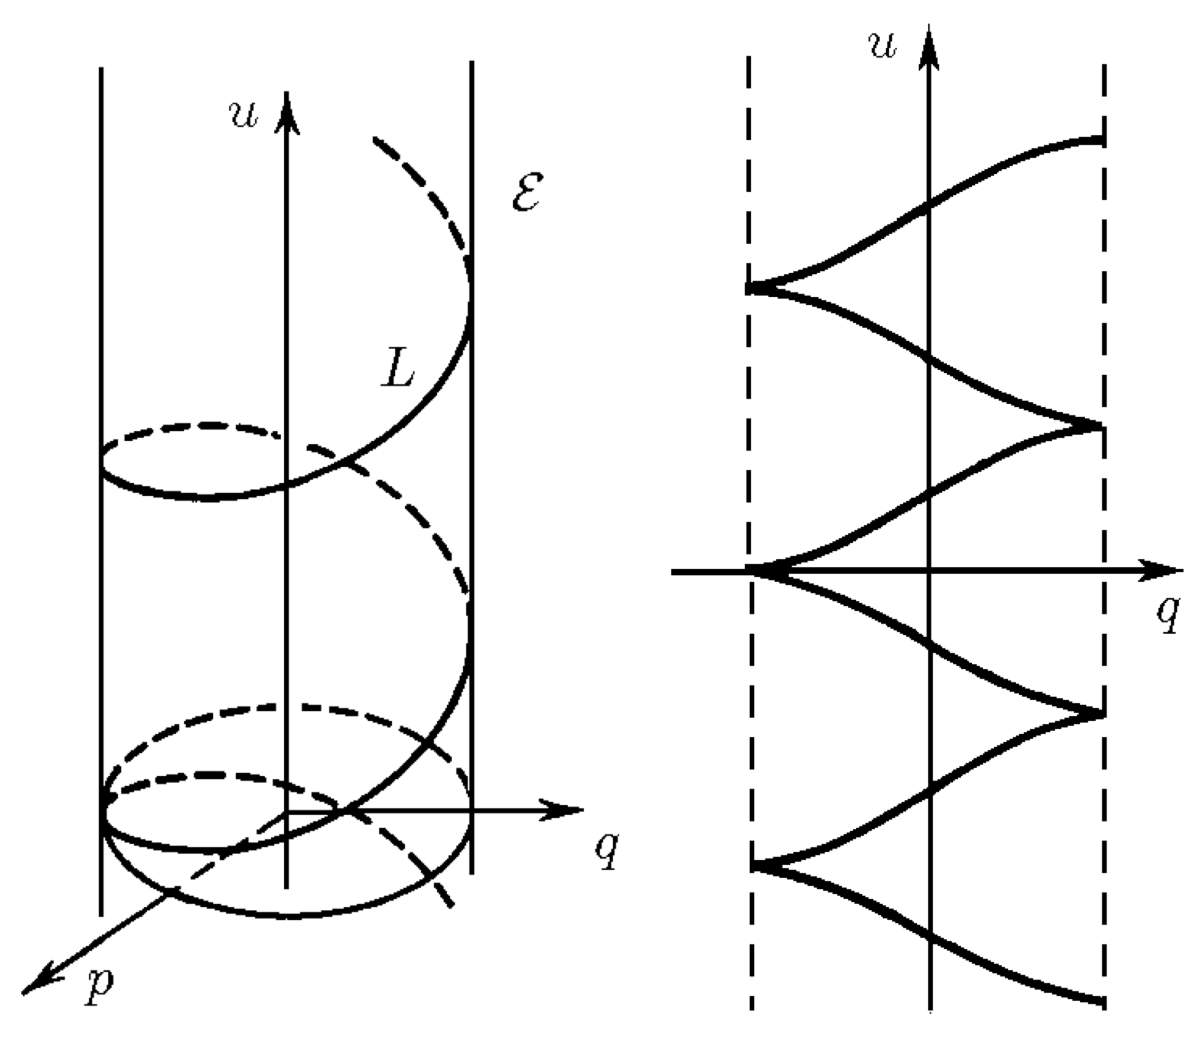
\includegraphics[scale=0.5]{figures/oscillator.png}
    \caption{A generalized trajectory of the harmonic oscillator and its projection to the $qu$-plane.}
    \label{fig:oscillator}
\end{figure}

\begin{example}
    Consider the stationary Hamilton-Jacobi equation 
    \[\left(\frac{\partial S}{\partial q}\right)^2+q^2=C=\const\]
    describing a $1$-dimensional harmonic oscillator. The corresponding locus $\calE:p^2+q^2=C$ is a cylinder in the $(q,u,p)$-space. The Cartan distribution $\calC(\calE)$ is a direction field on this cylinder, described by $\dd u=p\dd q$. Integral curves are generalized solutions of the equation. It is obvious that these curves project to the $q$-axis with degeneration, see Figure~\ref{fig:oscillator}.
\end{example}

In Theorem~\ref{thm 3.1.1 Kras} we showed that $r$-graphs of sections are integral manifolds of the Cartan distribution. Now we will describe the structure of arbitrary maximal integral manifolds.

\begin{defn}[Prolongation of submanifold]
    Let $P<\calC_p^{r-1}$ be a subspace of dimension $s\leq \dim M$. The subset 
    \[\ell(P)\coloneqq \{p'\in \rmJ^r E\mid P<L_{p'}\}\] 
    of the fiber over $p$ is called the \emph{ray submanifold} (or just \emph{ray}) corresponding to the subspace $P$. If $N<\rmJ^{r-1}E$ is a submanifold, then the set 
    \[L(N)\coloneqq \bigcup_{q\in N}\ell(\T_q N)\]
    is called the \emph{prolongation} (or \emph{lifting}) of the submanifold of $N$.
\end{defn}

The prolongation of $N$ consists of $r$-jets that are the possible derivatives of sections whose $(r-1)$-jets lie in $N$.

\begin{xca}
    Show that if $\graph^{r-1} (f)\subset N$, then $\graph^r(f)\subset L(N)$.
\end{xca}

\begin{example}
    Let $E=\bbR^2\times\bbR\to M=\bbR^2$. Consider an integral curve $Q$ of the Cartan distribution on $\rmJ^1E$ and its prolongation to $\rmJ^2E$. The prolongation is not empty iff the curve $Q$ is horizontal w.r.t.\ $\pi^1:\rmJ^1E\to \bbR^2$. Then we can choose coordinates $x,y$ on $\bbR^2$ such that the projection $S$ of $Q$ in a neighborhood of some point is of the form $y=0$.  The curve itself in this case can be described by relations of the form 
    \[y=0,\quad u=\alpha(x),\quad p=\beta(x),\quad q=\gamma(x).\]
    Since this curve is an integral manifold of the Cartan distribution given by $\restr{(\dd u-p\dd x-q\dd y)}{Q}=0$, one has $\beta=\alpha_x$. The relations above mean that we know the values of the function $u(x,y)$  together with the values of its derivative $u_y(x,y)$ for $y=0$. Thus we obtained the standard formulation for the Cauchy problem for second-order equations. Hence, in this situation the problem of prolongation is equivalent to describing the $2$-graphs of functions satisfying Cauchy conditions along $S$.

    Let $(x,y,u,p,q)\in Q$ and  let $\xi=(X,Y,U,P,Q)$ be a tangent vector. Let us describe the set $\ell(\xi)\subset (\pi^2_1)^{-1}(x,y,u,p,q)$. Denote by $r,s,t$ coordinates in the fiber of $\pi^2_1:\rmJ^2E\to \rmJ^1E$ (corresponding to $u_{xx},u_{xy},u_{yy}$). Then the equations 
    \[Xr+Ys=P,\quad Xs+Yt=Q\label{eq 3.2.8 Kras}\]
    describe the line $\ell(\xi)$. Note that the classical concept of a characteristic for second order equations is based on consideration of system \eqref{eq 3.2.8 Kras} together with the initial equation $\calE\subset\rmJ^2E$.
\end{example}

For clarity let us denote by $\calC^r$ the Cartan distribution on $\rmJ^r E$.

\begin{cor}
    For an integral manifold $N\embweak\rmJ^{r-1}E$ of $\calC^{r-1}$ transverse w.r.t.\ the projection $\pi^{r-1}$ to the base, the corresponding prolongation $L(N)\subset \rmJ^rE$ is an integral manifold of $\calC^r$.
\end{cor}
\begin{proof}
    It suffices, applying Theorem~\ref{thm 3.2.1 Kras}, to check that at any $p'\in L(N)$ the image of $\T_{p'}L(N)$ under $\pi^r_{r-1}$ lies in $L_{p'}$. By definitions and the construction of $L(N)$, we have $(\pi^r_{r-1})_{\ast p'}L(N)=\T_{p'}L(N)=\T_pN< L_{p'}$. Thus, $L(N)$ is an integral manifold.
\end{proof}

As we will prove below, the above construction is of a universal nature. We now describe the local structure of transverse integral manifolds $N$ and deduce a formula to compute $\dim L(N)$ in terms of $\dim N$.

\begin{prop}[{\cite[Prop.~3.2.4]{Kras}}]\label{prop 3.2.4 Kras}
    Any transverse integral manifold $N$ of the Cartan distribution on $\rmJ^rE$ locally lies in the $r$-graph $\graph^r(s)$ of some section $s$.
\end{prop}
\begin{proof}
    Let $l=\dim N\leq n$ and $\rank E=k$. Let us introduce in a neighborhood of the point $m=\pi^r(p)$, $p\in N$, coordinates $x^1,\ldots,x^n$ such that $\underline{N}=\pi^r(N)$ is given by the equations $x^{l+1}=\cdots=x^n=0$. Since the manifold $N$ is transverse, it is described by the equations 
    \[x^i=0,\; i>l,\quad p^j_I=\underline f^j_I(\bf{x}),\; j=1,\ldots,k,\; |I|\leq r.\]
    Restricting the contact forms to $N$ (cf. the proof of Theorem~\ref{thm 3.1.1 Kras}), we obtain that 
    \[\underline f^j_{I+1_i}=\frac{\partial\underline f^j_I(x^1,\ldots,x^l)}{\partial x^i},\quad |I|\leq l-1,\quad i=1,\ldots,l.\]
    Thus, the functions $\underline f^1,\ldots,\underline f^k$ are defined on $\underline{N}$. They satisfy the above conditions and the values of all their normal derivatives are given along $\underline{N}$. Hence, there exist functions $f^1,\ldots,f^k$ such that $\restr{f^j}{\underline{N}}=\underline{f}^j$ and with the given values of normal derivatives on $\underline{N}$. Consequently, $\bf{f}(\bf{x})=(f^1,\ldots,f^k)$ is the section we need.
\end{proof}

\begin{prop}[{{\cite[Prop.~3.2.5]{Kras}}}]\label{prop 3.2.5 Kras}
    Let $\pi:E\to M$ be a rank $k$ \gls{vb} over an $n$-dimensional manifold $M$ and $N\embweak \rmJ^r E$ a transverse integral manifold of dimension $l\leq n$ of the Cartan distribution. Then 
    \[\dim L(N)=l+k\binom{n-l+r}{n-l-1}.\]
\end{prop}

\begin{cor}\label{cor 3.2.6 Kras}
    If $l_1=\dim N_1<l_2=\dim N_2$, then $\dim L(N_1)\geq \dim L(N_2)$ and equality is achieved only in the following cases:
    \begin{enumerate}[label=(\alph*)]
        \item $k=n=1$.
        \item $r=0,k=1$.
        \item $k=1$, $l_1=n-1$, $l_2=n$.
    \end{enumerate}
\end{cor}

\begin{thm}[{\cite[Thm.~3.2.7]{Kras}}]\label{thm 3.2.7 Kras}
    An integral manifold $Q$ of the Cartan distribution on $\rmJ^r E$ is maximal iff everywhere, except possibly for a manifold of lower dimension, it is locally of the form $L(N)$ for some transverse integral manifold $N\embweak\rmJ^{r-1}E$. 
\end{thm}
\begin{proof}
    Let $Q\embweak \rmJ^rE$ be a maximal integral manifold of $\calC^r$. We shall prove the theorem for any point $p\in Q$ such that in its neighborhood the rank of $\pi^r_{r-1}$ is constant (clearly, such points form an open everywhere dense set in $Q$). The following lemma follows from the \gls{immt} and is given without proof.

    \begin{lem}
        Let $A,B$ be smooth manifolds and $f:A\to B$ be a smooth mapping of constant rank $p$ in a neighborhood of a point $a\in A$. Then there exists a neighborhood $U\ni a$ such that the set $f(U)$ is a submanifold in a neighborhood of $b=f(a)$. Moreover, its tangent space at $b$ is the image of the tangent space of $A$ at $a:\T_b (f(U))=f_\ast(\T_a A)$.
    \end{lem}

    Now let $p\in Q$ and $N=\pi^r_{r-1}(U)$ be the projection of the corresponding neighborhood $U\subset Q$ to $\rmJ^{r-1}E$. By the lemma, $N$ is submanifold in $\rmJ^{r-1}E$. Let $p'=\pi^r_{r-1}(p)$. By the same lemma and by Theorem~\ref{thm 3.2.1 Kras}, one has $\T_{p'}(N)=\T_{p'}(\pi^r_{r-1}(Q))=(\pi^r_{r-1})_\ast (\T_p Q)\subset (\pi^r_{r-1})_\ast (\calC^r_p)=L_p$. It follows that $N$ is a transverse manifold and $\dim N\leq n$, and we can apply Proposition~\ref{prop 3.2.4 Kras}. The embedding $L_p\emb \T_{p'}N$, by definition, means that $p\in L(N)$. Hence, $U\subset L(N)$, i.e., $Q\subset L(N)$ locally. Therefore, by maximality, $Q=L(N)$.

    Conversely, consider a manifold of the form $L(N)$. As it was just proved, it contains in the maximal integral manifold $L(N_1)$ and $\dim L(N)\leq \dim L(N_1)$. But $N=\pi^r_{r-1}(L(N))$, $N_1=\pi^r_{r-1}(L(N_1))$. Therefore, $N\subset N_1$ and $\dim N\leq \dim N_1$. By Corollary~\ref{cor 3.2.6 Kras}, one has $\dim L(N_1)\leq \dim L(N)$, i.e., $L(N)=L(N_1)$.
\end{proof}

Note that if $N$ is the $(r-1)$-graph of some section of $E$, then the manifold $L(N)$ is the $r$-graph of the same section. Hence, $r$-graphs of sections are maximal integral manifolds of $\calC^r$.

From the above theorem and Corollary~\ref{cor 3.2.6 Kras}, we get the following.

\begin{cor}[{\cite[Cor.~3.2.9]{Kras}}]\label{cor 3.2.9 Kras}
    Except for the cases $k=n=1$ ($1$ function of $1$ variable) and $r=k=1$ ($1$-jets of $1$ function), manifolds of the form $L(N)$, where $\dim N=0$, are of the maximal dimension among all integral manifolds of $\calC^r$. In other words, the fibers of $\pi^r_{r-1}$ are the only integral manifolds of maximal dimension.
\end{cor}

This fact is of fundamental importance in the description of the symmetries of the Cartan distribution, which we do next.







\section{Contact transformations}

The following important notion of symmetries of the Cartan distribution (or the dual contact system) underlies Lie's original theory of symmetries of differential equations, which was developed as a continuum analog of the Galois theory of symmetries of algebraic equations.

\begin{defn}[Contact transformation, Prolongation, Point symmetry]\index{Lie transformation}\index{Point transformation}\index{Contact transformation}\index{Prolongation}
    A ($r$-th order) contact transformation, or a contactomorphism (also sometimes called Lie transformations), on a jet bundle $\rmJ^r E$ of a \gls{vb} $E\to M$, is a symmetry of the Cartan distribution $\calC^r$.

    The \emph{$(r+q)$-th order prolongation} $F^{(q)}$ of a contact transformation $F:\rmJ^rE\to \rmJ^rE$ is the unique contact transformation on $\rmJ^{r+q}E$ which projects back to $F$, i.e., $\pi^{r+q}_r\circ F^{(q)}=F\circ \pi^{r+q}_r$.

    Prolongations of diffeomorphisms of $E$ are called \emph{point transformations} (they are obviously contact transformations).
\end{defn}

\begin{rem}
    Let us give an explicit description of the prolongation. Let $F:E\to E$ be a diffeomorphism and let $p\in \rmJ^r E$, $\pi^r_0(p)=e\in E$, $\pi^r(p)=m\in M$. Choose a section $s\in\Gamma^\infty(E)$ such that $p=\rmj_m^r s$ and consider its graph $\graph(s)\subset E$. If, in a neighborhood of $e'=F(e)$, the image $F(\graph(s))$ is the graph of some section $s'$, we shall define $p'\coloneqq \rmj_{m'}^r s'$, where $m'=\pi(e')$ and define the $r$-th order prolongation of $F$ by $F^{(r)}(p)\coloneqq p'$.
\end{rem}

\begin{xca}
    \begin{enumerate}
        \item In the above remark, show that the point $p'$ is independent of the choice of the section $s'$, given $p$.
        \item Show that if $F^{(1)}$ is defined around some point $p\in \rmJ^1E$, then $F^{(r)}$ is defined around any point $p'\in \rmJ^rE$ lying above $p$ (w.r.t.\ $\pi^r_1$).
        \item Show that, where $F^{(r+s)}$ is well-defined, the equality $\left(F^{(r)}\right)^{(s)}=F^{(r+s)}$ holds.
    \end{enumerate}
\end{xca}

\begin{example}[Point transformations]
    \begin{enumerate}
        \item The translation along a constant vector field in $\bbR^n\times\bbR^k$ is a point transformation described by 
        \[x^i\mapsto x^i+\xi^i,\quad u^j\mapsto u^j+\eta^j.\]
        It acts as the identity on all variables $p^j_I$.
        \item A Galilean transformation on the space of functions $u(t,x)$ is given by 
        \[t\mapsto t,\quad x\mapsto x-vt,\quad u\mapsto u.\]
        The prolongation of this to $1$-jets is of the form 
        \[u_t\mapsto u_t+vu_x,\quad u_x\mapsto u_x.\]
        \item An arbitrary diffeomorphism of the plane $(x,u)\mapsto (\lambda(x,u),\mu(x,u))$ induces a \gls{flt} in $p$ of the $3$-dimensional $(x,u,p)$-space. It is easily checked that
        \[p\mapsto \frac{\dd \mu}{\dd \lambda}=\frac{\mu_x\dd x+\mu_u\dd u}{\lambda_x\dd x+\lambda_u\dd u}=\frac{\mu_x+\mu_up}{\lambda_x+\lambda_up}.\]
        \item For a general point transformation 
        \[\wb{\bf{x}}= \bf{f}(\bf{x},\bf{u}),\quad \wb{\bf{u}}=\bf{g}(\bf{x},\bf{u}),\]
        its prolongation to the space of $1$-jets $p^i_j\mapsto \wb p^{i}_j$ is given by the system of $n k$ linear equations 
        \[\sum_{l=1}^n D_i(\wb x^{ l})\wb p_l^{j}=D_i(\wb u^{j}),\quad i=1,\ldots,n,\; j=1,\ldots,k,\]
        where $D_i$ is the \emph{total derivative operator} along $x^i$, defined by \index{Total derivative operator}
        \[(D_i f)(\bf{x},\bf{u},\bf{p})\coloneqq\frac{\partial f}{\partial x^i}+\sum_{j=1}^k p^j_i\frac{\partial f}{\partial u^j}.\label{def total deriv}\]
        (Note that it produces a function of 1-jets; its extensions to higher-order jets will be defined below.) The determinant of the matrix $\{D_i(\wb x^{j})\}_{i,j}$ is unsurprisingly called the ``total Jacobian'' of the system of functions $\wb x^{j}$. Note that the vanishing of this Jacobian on some open set implies functional dependence of the functions $\wb x^{j}$. Since the point transformation is a local diffeomorphism, the Jacobian is almost never zero, so the above linear equations determine the $\wb p^{j}_i$ uniquely almost everywhere.
    \end{enumerate}
\end{example}


\begin{example}[Legendre transform]
    Not every contact transformation is a point transformation. Let $E=\bbR^n\times \bbR\to M=\bbR^n$ and consider the \emph{Legendre transformation} \index{Legendre transform}
    \[\mathscr{L}:\quad x^i\mapsto p_i,\quad u\mapsto \sum_{j=1}^n x^jp_j-u,\quad p_i\mapsto x^i,\quad i=1,\ldots,n,\]
    where $x^1,\ldots,x^n,u,p_1,\ldots,p_n$ are the canonical coordinates. It is easy to check that this preserves the Cartan distribution.
\end{example}

\begin{xca}[{{\cite[Exercise~4.31]{OlverEquiv}}}]\label{xca 4.31 OlverEquiv}
    Suppose $\varPsi:\rmJ^1E\to \rmJ^1E$ is a contact transformation with local coordinate expression $\wb x^i=\chi^i(\bf{x},\bf{u},\bf{p})$, $\wb u^a=\psi^a(\bf{x},\bf{u},\bf{p})$, $\wb p^a_i=\pi^a_i(\bf{x},\bf{u},\bf{p})$. First show that 
    \[\sum_{i=1}^n \pi^a_i D_j\chi^i=D_j\psi^a.\]
    Then prove that the associated action on the basic contact forms is 
    \[\varPsi^\ast(\wb\theta^a)=\sum_{b=1}^k\left(\frac{\partial\psi^a}{\partial u^b}-\sum_{i=1}^n \pi^a_i\frac{\partial \chi^i}{\partial u^b}\right)\theta^b.\]
    Can you extend this result to higher-order contact forms?
\end{xca}

Defining the notion of symmetry for a differential equation $\calE$ is a subtle undertaking, and as a result there are many different types of symmetries. Conceptually, the most natural definition would be as a diffeomorphism of $\calE$ that preserves the restricted Cartan distribution $\calC(\calE)$ (an \emph{internal symmetry}). However, computations are much simpler if one takes the broader point of view from the ambient jet bundle. The following class of symmetries may also be called \emph{external}.

\begin{defn}[Equivalent equations, Contact symmetry]\index{Contact symmetry}
    Two equations $\calE,\calE'\subset\rmJ^r E$ are called (locally) equivalent if there is a contact transformation $F\in\Aut(\calC^r)$ such that the image of $\calE$ is $\calE'$. The transformation $F$ is called a \emph{contact, or classical, symmetry} of $\calE$ if $F(\calE)=\calE$.
\end{defn}

The next few examples show the power of contact symmetries for solving differential equations. Note, however, that they belong to the special case $r=k=1$, where the maximal-dimensional integral manifolds of the Cartan distribution are not necessarily vertical, which makes symmetries much more useful for solving equations.

\begin{example}[Legendre transform]\index{Legendre transform}
    The Legendre transform is a contact symmetry of the equation 
    \[\calE=\left\{u-\frac12\sum_{i=1}^n x^ip_i=0\right\}.\]
    This equation is solved by any smooth homogeneous function of degree $2$. In particular, it has the $n$-parameter family of solutions $u=\sum_{i=1}^n b_i(x^i)^2$, where $b_i\in\bbR$. This family is invariant under the Legendre transform:
    \[\mathscr{L}\left(\rmj^1\left(\sum_i b_i(x^i)^2\right)\right)=\rmj^1\left(\sum_i \frac{(x^i)^2}{4b_i}\right).\]
    The $1$-graph of the constant function $u=c$ transformed by the Legendre transform $\{u=c,\bf{p}=0\}\mapsto \{u=-c,\bf{x}=0\}$ is an integral manifold whose projection to the manifold of independent variables is the point $\bf{x}=0$.
\end{example}

As the above example shows, finding a contact transformation that maps the equation to one that doesn't depend on the derivatives (i.e., is a subbundle of jets) is as good as solving the equation. In the next two examples we give an explicit example.

\begin{example}[Clairaut equations]\index{Equation!Clairaut}
    The general \emph{Clairaut equation} has the form 
    \[\calE:\quad F\left(\sum_i x^ip_i-u,p_1,\ldots,p_n\right)=0,\]
    where $F$ is a smooth function of $n+1$ variables. The image of this equation under the Legendre transform is the equation 
    \[\calE'=\mathscr{L}(\calE):\quad F(u,x^1,\ldots,x^n)=0,\]
    which contains no derivatives. $\calE'$ is an $n$-dimensional surface in the $(n+1)$-dimensional space $E=\bbR^n\times\bbR$, the corresponding first-order differential equation being its preimage under the projection $\pi^1_0:\rmJ^1E\to E$.

    Take a point $(a_1,\ldots,a_n,b)\in E$ such that $F(b,a_1,\ldots,a_n)=0$. The fiber of $\pi^1_0$ over this point is a generalized solution of $\calE'$. Applying the Legendre transformation to these generalized solutions yields an $n$-parameter family of single-valued solutions of $\calE$, which is hence a \emph{complete integral} of the Clairaut equation.

    On the other hand, solving $\calE'$ for $u$ in the vicinity of a nonsingular point (where $F_u\neq 0$) yields 
    \[u=f(x^1,\ldots,x^n).\]
    To find the image of this solution under the Legendre transformation observe that the $1$-graph of $f$ has the form 
    \[p_i=f_{x^i}(\bf{x}),\quad F(u,x^1,\ldots,x^n)=0.\]
    Under the Legendre transform, this maps to the system 
    \[x^i=f_{x^i}(\bf{p}),\quad F\left(\sum_i x^ip_i-u,p_1,\ldots,p_n\right)=0,\]
    which is compatible. Express $\bf{p}$ in terms of $\bf{x}$ via the first equation. Substituting into the last equation and solving for $u$ in terms of $\bf{x}$ yields a discrete set of solutions to the Clairaut equation, which are called \emph{exceptional integrals}.
\end{example}

\begin{example}
    Consider the following Clairaut equation with two independent variables 
    \[\calE:\quad xp_x+yp_y-u=\frac13(p_x^3+p_y^3).\]
    Using the Legendre transform, we obtain $\calE':u=\frac13(x^3+y^3)$, which gives the following complete integral of the original equation:
    \[u=a_1x+a_2y-\frac13(x^3+y^3),\quad a_1,a_2=\const.\]
    Exceptional integrals are found from the system 
    \[u=xp_x+yp_y-\frac13(p_x^3+p_y^3),\quad x=p_x^2,\quad y=p_y^2.\label{eq 1.1.25 Kras}\]
    It follows that exceptional integrals exist in the quadrant $x>0,y>0$ and have the form 
    \[p_x=\alpha_1\sqrt{x},\quad p_y=\alpha_2\sqrt{y},\quad u=\frac23(\alpha_1x^{3/2}+\alpha_2y^{3/2}),\label{eq 1.1.26 Kras}\]
    with $\alpha_1,\alpha_2\in \{-1,1\}$. This formula defines $4$ exceptional integrals. However, from the geometric point of view, the system \eqref{eq 1.1.25 Kras} defines only one generalized solution, which is a surface of the fourth order and degenerately projecting to the $\bf{x}$-plane. Formula \eqref{eq 1.1.26 Kras} defines the four branches of this generalized solution.
\end{example}

The following surprising theorem gives a complete description of contact transformations.

\begin{thm}[B\"acklund (1876) {{\cite[Thm.~3.3.1]{Kras}}}]\label{thm 3.3.1 Kras}
    Any contact transformation $F$ of the jet space $\rmJ^rE$, $r\geq 1$, is described as follows:
    \begin{enumerate}
        \item For $\rank E=1$, the transformation $F$ is the $(r-1)$-st prolongation of some contact transformation of $\rmJ^1E$.
        \item For $\rank E=k>1$, the transformation $F$ is the $r$-th prolongation of a diffeomorphism of $E$, i.e., $F$ is a point transformation.
    \end{enumerate}
\end{thm}
\begin{proof}
    The proof is based on the above established fact: the fibers of $\pi^r_{r-1}$ are integral manifolds of maximal dimension of the Cartan distribution $\calC^r$ when $kn>1$ and $rk>1$ (cf.\ Corollary~\ref{cor 3.2.9 Kras}). The case $r=k=1$ is tautological. The case $k=n=1$ needs a special treatment.

    Assume that $kn>1$ and $rk>1$. Let $F:\rmJ^rE\to \rmJ^rE$ be a contact transformation. Since $F$ preserves the Cartan distribution, it must take its maximal integral manifolds to maximal integral manifolds. Since $F$ is a diffeomorphism, the dimension of these manifolds is preserved. Consequently, according to Corollary~\ref{cor 3.2.9 Kras}, $F$ takes a fiber of $\pi^r_{r-1}$ to another fiber. Hence, $F$ induces a transformation $\underline{F}$ of $\rmJ^{r-1}E$: if $F\left((\pi^r_{r-1})^{-1}(p)\right)=(\pi^r_{r-1})^{-1}(p')$ for $p,p'\in\rmJ^{r-1}E$, then $\underline{F}(p)=p'$.

    Since $\underline{F}$ is the projection of the contact transformation $F$, it is itself a contact transformation. Let us consider the transformation $F$ and the prolongation $\underline{F}^{(1)}$ of $\underline{F}$. They both are symmetries of the Cartan distribution $\calC^r$, preserve the fibers of $\pi^r_{r-1}$, and induce the same transformation of $\rmJ^{r-1}E$. Therefore, the diffeomorphism $F'\coloneqq F^{(1)}\circ F^{-1}$ is a contact transformation of $\rmJ^rE$ inducing the identity map on $\rmJ^{r-1}E$.

    \begin{xca}
        Prove that a contact transformation of $\rmJ^rE$ that projects to the identity map on $\rmJ^{r-1}E$ must be the identity map.
    \end{xca}

    By the above exercise, $F=\underline{F}^{(1)}$. Applying the same argument inductively, we obtain some transformation $f$ of $\rmJ^1E$ if $k=1$ or of $\rmJ^0E=E$ if $k>1$. To conclude the proof, it suffices to use the property $(f^{(r)})^{(s)}=f^{(r+s)}$.

    In the case $k=n=1$, the proof is implied by the following considerations. Let $x,p_0,\ldots,p_r$ be canonical coordinates on $\rmJ^r(\bbR,\bbR)$. The Cartan distribution $\calC$ on $\rmJ^r(\bbR,\bbR)$ is of rank $2$, generated by the vector fields $Z=\partial/\partial p_r$ and $D=\partial_x+\sum_{i=1}^{r-1}p_{i+1}\partial/\partial p_i$. It suffices to prove that any contact transformation $F$ takes $Z$ to itself; all further reasoning will be similar to the above used. Denote by $V$ the rank $1$ distribution spanned by $Z$.

    \begin{lem}
        Let $\calC'=[\calC,\calC]$ be the distribution on $\rmJ^r(\bbR,\bbR)$, $r\geq 2$, spanned by the commutators of elements of $\Gamma^\infty(\calC)$. Then, denoting by $\calC_D$ the normalizer of the set $\Gamma^\infty(\calC)$ within the Lie algebra of all vector fields, i.e.,
        \[\calC_D=\{X\in \fX(\rmJ^r(\bbR,\bbR))\mid [X,\Gamma^\infty(\calC)]\subset  \Gamma^\infty(\calC)\},\]
        one has 
        \[\Gamma^\infty(V)=\Gamma^\infty(\calC)\cap \calC_D'.\]
    \end{lem}
    \begin{proof}[Proof of the lemma]
        Obviously, the distribution $\calC'$ is of rank $3$. It is spanned by the fields $Z,D$, and $[Z,D]=\partial/\partial p_{r-1}\eqqcolon Y$. It is easily seen that $[Z,Y]=0$, $[Y,D]=X=\partial/\partial p_{r-2}$. Let the field $S\coloneqq \alpha Z+\beta D$ be a symmetry of $\calC'$. Then $[Y,S]\in\Gamma^\infty(\calC')$, i.e., $[Y,S]$ is represented as a linear combination of $Z,D,Y$. But since 
        \[[Y,S]=[Y,\alpha Z+\beta D]=Y(\alpha)Z+Y(\beta)D+\beta X,\]
        and the fields $X,D,Z$ are linearly independent at all points, we obtain $\beta=0$. Hence, $S\in\Gamma^\infty(V)$.
    \end{proof}
    Let now $F:\rmJ^r(\bbR,\bbR)\to \rmJ^r(\bbR,\bbR)$. Then, obviously, $F_\ast \Gamma^\infty(\calC)=\Gamma^\infty(\calC)$, $F_\ast\calC'=\calC'$ and $F_\ast \calC_D'=\calC_D'$. Then, by the lemma, one has $F_\ast \Gamma^\infty(V)=\Gamma^\infty(V)$. The theorem is proved.
\end{proof}

\begin{rem}
    In fact, B\"acklund proved this result not just for infinitesimal transformations, but for actual contact transformations. The restrictions imposed by B\"acklund's theorem severely limit the range of applicability of contact transformations. The core issue is that we have been considering symmetries of the full Cartan distribution $\calC$, whereas for a particular differential equation $\calE$ only the restricted distribution $\calC(\calE)$ matters. It is possible that $\calC(\calE)$ possesses additional non-contact higher-order symmetries, known as \emph{internal symmetries}, which are not merely restrictions of contact transformations of the jet bundle. We will not consider such symmetries here and instead direct the reader to \cite[\S3.7]{Kras} and \cite{Olver93}.
\end{rem}


\begin{defn}[Contact vector field]\index{Lie vector field}\index{Contact vector field}
    A vector field $X\in\fX(\rmJ^r E)$ is called a ($r$-th order) contact, or \emph{Lie}, vector field, if its flow boxes are local contact transformations, i.e. $[X,\Gamma^\infty(\calC^r)]=0$. 
    
    For an equation $\calE\subset\rmJ^rE$, a contact vector field $X\in\fX(\rmJ^r E)$ is called a \emph{classical infinitesimal symmetry} if it is tangent to $\calE$.
\end{defn}

Let $X$ be a contact vector field on $\rmJ^r E$. In the same way as we defined prolongations for diffeomorphisms of $\rmJ^r E$, we can define prolongations of vector fields by prolonging their (local if incomplete) flows. We denote the resulting vector fields by $X^{(l)}\in \fX(\rmJ^{r+l}E)$, $l\geq 1$. Again, $\left(X^{(l)}\right)^{(s)}=X^{(l+s)}$. Also, since prolongation respects the composition of maps, and the commutator of the flows is generated by the Lie bracket of the vector fields, prolongation is a Lie algebra homomorphism:
\[[X^{(r)},Y^{(r)}]=[X,Y]^{(r)}.\label{eq prolongation lie hom}\]
The above theorem implies the following infinitesimal analog.

\begin{thm}\label{thm 3.3.3 Kras}
    Any contact vector field $X\in\fX(\rmJ^rE)$, $r\geq 1$, is of the form:
    \begin{enumerate}[label=(\alph*)]
        \item $X^{(r)}$ if $\rank E>1$, where $X\in\fX(E)$.
        \item $X^{(r-1)}$ if $\rank E=1$, where $X$ is a contact vector field on $\rmJ^1 E$.
    \end{enumerate} 
\end{thm}

Note that any contact vector field on $\rmJ^1E$ can be lifted to a Lie field on any $\rmJ^r E$ by prolongation. Also, unlike for contact transformations, the prolongation of contact vector fields is always well-defined globally, since it suffices to know an arbitrarily small part of the integral curve of $X^{(1)}$ through a point, and R-planes necessarily get mapped to R-planes by the flow $\Fl^X_t$ for sufficiently small $t$.

Another advantage of contact vector fields is that there are explicit formulas for their prolongations, and one can use the techniques of generating functions (see below). To this end, we first note that a vector field $X\in\fX(\rmJ^r E)$ is a contact vector field iff its inner product with any of the standard contact forms $\theta^j_I$ satisfies
\[\Lie_X \theta^j_I=\sum_{l=1}^k\sum_{|K|\leq r-1}\lambda^{jK}_{Il}\theta^l_K\] 
for some set of functions $\lambda^{jK}_{Il}$.

\begin{defn}[Total derivative operator]\index{Total derivative operator}
    Fixing a bundle $E\to M$ of rank $k$ with coordinates $(\bf{x},\bf{u})$ as above, the total derivative operators $D_i$, $i=1,\ldots,n$, acting on functions on any jet bundle $\rmJ^rE$ and producing functions on $\rmJ^{r+1}E$ are defined in canonical coordinates by 
    \[D_i \coloneqq \frac{\partial}{\partial x^i}+\sum_{j=1}^k\sum_{I}p_{I+1_i}^j\frac{\partial}{\partial p^j_I}.\label{eq def total derivative}\]
    Here, $I$ ranges over all possible multi-indices, so this can be considered an infinite-order operator, but when acting on $\rmJ^r E$, only the terms with $|I|\leq r$ contribute.
\end{defn}

\begin{thm}[Prolongation formula {{\cite[Thm.~3.3.4]{Kras}}}]\label{thm 3.3.4 Kras}
     Let 
     \[X=\sum_{i=1}^n a^i \frac{\partial}{\partial x^i}+\sum_{j=1}^k \sum_{|I|\leq r}b^j_I \frac{\partial}{\partial p^j_I}\] 
     be a contact vector field on $\rmJ^r E$. Then the first-order coefficients $a^i$ and $b^j_i$ depend at most only on the $1$-jets $(x^i,u^j,p^j_i)$ (and if $\rank E>1$, then only on the $0$-jets $(x^i,u^j)$), and the higher-order coefficients $b^j_I$, $0\leq |I|\leq r-1$, $j=1,\ldots,k$, are computed by the recurrent formulas 
     \[b^j_{I+1_i}=D_i(b^j_I)-\sum_{s=1}^n p^j_{I+1_s}D_i(a^s),\quad 0\leq |I|\leq r-1,\; i=1,\ldots,n. \label{eq 3.3.9 Kras}\]
    Moreover, $X$ is a point vector field iff the $a^i$ are independent of the $p^j_I$.
\end{thm}
\begin{proof}
    By the invariance of the Cartan distribution, the forms 
    \[\Lie_X \theta^j_I=(\dd i_X+i_X\dd)\left(\dd p^j_I-\sum_i p^j_{I+1_i}\dd x^i\right)=\dd b^j_I-\sum\left(b^j_{I+1_i}\dd x^i+p^j_{I+1_i}\dd a^i\right)\label{eq 3.3.10 Kras}\]
    are still contact forms.  According to Remark~\ref{rem semibasic and contact forms}, for any smooth function $\varphi$ on $\rmJ^rE$ one can locally decompose its differential into semibasic and contact components as
    \[\dd \varphi=\sum_i D_i(\varphi)\dd x^i+\sum_{j,I}\frac{\partial\varphi}{\partial p^j_I}\theta^j_I.\]
    Note that $\dd\varphi$ vanishes on the Cartan distribution iff the first term is zero. Applying this observation to \eqref{eq 3.3.10 Kras}, we obtain 
    \[\Lie_X \theta^j_I=\sum_i \left(D_i(b^j_I)-b^j_{I+1_i}-\sum_s p^j_{I+1_i}D_i(a^s)\right)\dd x^i+\theta\]
    for some contact form $\theta$. Since this must be a contact form, the first (semibasic) term must vanish, implying \eqref{eq 3.3.9 Kras}.
\end{proof}

Thus, a contact vector field is a point vector field iff it depends on the $p$-variables only in a prescribed polynomial way. In particular, it has to depend on the first-order derivatives $p^j_i$ affinely.

This exercise, combined with the fact that all contact vector fields are the prolongations of at most first-order contact vector fields, means that all contact vector fields are fully parametrized by some set of coefficients that are functions on $\rmJ^1E$. These coefficients can be formed into a single geometric object. To this end, we now introduce the concept of the \emph{generating section} of a contact vector field. 

Consider the evolution of the graphs of sections of $E$ under the action of the corresponding \gls{ops} of (local) contact transformations. Let $X=a^i\partial_{x^i}+b^j\partial_{u^j}+\cdots $ be a contact vector field on $\rmJ^r E$ and let $F_t$ be the corresponding local flow. Consider a local section $s\in\Gamma^\infty(E)$. The $r$-graph $\graph^r(s)\subset \rmJ^rE$ is a transverse $n$-dimensional integral manifold of the Cartan distribution on $\rmJ^rE$. As was already pointed out, for sufficiently small $t$, the manifold $F_t(\graph^r(s))$ is also an $r$-graph of some other local section $s_t$:
\[F_t(\graph^r(s))=\graph^r(s_t).\]

Thus, the contact transformations $F_t$ generate the evolution $s_t$ of $s$. Let us find the velocity $\dot s_t$ of this evolution at $t=0$. To compute it, let us represent $X$ as the sum of two fields
\[X=X_1+Y,\quad X_1\in\Gamma^\infty(\calV\rmJ^r E),\quad Y\in\fX(\graph^r(s)),\]
one vertical and the other tangent to $\graph^r(s)$. If $s$ is locally represented by $u^j=s^j(\bf{x})$, $j=1,\ldots,k$, then a basis of vector fields tangent to $\graph^r(s)$ can be written in the following form (note that $p^j_I=\partial^{|I|}s^j/(\partial \bf x)^I$ on this manifold):
\[D_i^{(s)}=\frac{\partial}{\partial x^i}+\sum_{j=1}^k \left(\sum_{|I|< r}p^j_{I+1_i}\frac{\partial}{\partial p^j_I}+\sum_{|I|=r}\frac{\partial^{|I|+1}s^j}{(\partial \bf x)^I\partial x^i}\frac{\partial}{\partial p^j_I}\right).\]
Therefore, a vector field tangent to the $r$-graph is of the form 
\[Y=\sum_i a^i D_i^{(s)},\]
while the vertical component of the contact vector field $X$ equals 
\[X_1=X-\sum_i a^i D_i^{(s)}=\sum_j\left(b^j-\sum_i a^ip^j_i\right)\frac{\partial}{\partial u^j}+\cdots.\]
Since $Y$ shifts the manifold $\graph^r(s)$ along itself, it does not influence the evolution. On the other hand, the coefficients of the field $X_1$ at $\partial/\partial u^j$ exactly coincide with the velocities of the components of $s_t$:
\[\dot s^j_0=\restr{\left(b^j-\sum_i a^i p^j_i\right)}{\graph^r(s)}.\]
Recall from Theorem~\ref{thm 3.3.4 Kras} that $a^i,b^j$ depend (at worst) only on $1$-jets, so these velocities actually depend only on the $1$-graph of $s$. Moreover, they are exactly the coefficients of $\partial_{u^j}$ in $X_1$. Thus, they can be interpreted as the components of a section of the pullback bundle $(\pi^1_0)^\ast E\to \rmJ^1 E$ whose fiber over a point $p\in \rmJ^1 E$ is a copy of the corresponding fiber $\pi^{-1}(\pi^1_0(p))$ of $E$. 
% Note that these are exactly the vertical components of the projected vector field $(\pi^r_0)_\ast X_1\in\fX(E)$. Since the vertical bundle of a \gls{vb} $E$, restricted to a section, can be canonically identified with $E$ itself, $s^\ast \calV E\cong E$, these velocities describe a unique section of $E$. Since the values of the velocities don't depend on the choice of the section $s$ (only on the point in its graph), by applying this procedure to arbitrary sections of $E$, we get an $E$-valued $0$-form on $E$, i.e., a section of the pullback of $E$ along itself.

\begin{defn}[Generating section]
    Let $\pi:E\to M$ be a \gls{vb} of rank $k$. The section $\varphi\in\Gamma^\infty((\pi^1_0)^\ast E)$ whose components (in any local frame of $E$ and its lift) are 
    \[\varphi^j=\theta^j_{(0,\ldots,0)}(X)=b^j-\sum_i a^ip^j_i,\quad j=1,\ldots,k,\]
    is called the \emph{generating section}, or the \emph{characteristic}, of the first-order contact vector field 
    \[X=\sum_{i=1}^n a^i \frac{\partial}{\partial x^i}+\sum_{j=1}^k b^j\frac{\partial}{\partial u^j}+\cdots=\sum_j \varphi^j \frac{\partial}{\partial u^j}+Y,\quad \theta^j_{(0,\ldots,0)}(Y)=0.\]
    Upon restriction to the $1$-graph of a section of $E$, the resulting vertical vector field $X_1\coloneqq \sum_j \varphi^j \frac{\partial}{\partial u^j}$ on $E$ is called the \emph{evolutionary component} of $X$.
\end{defn}

By virtue of Theorem~\ref{thm 3.3.3 Kras}, each contact vector field is uniquely determined by its generating section. Indeed, if $k>1$, this is obvious since the $a^i$ and $b^j$ provide the components of the point vector field whose prolongation recovers $X$. In the case $k=1$, $a^i$ and $b^j$ determine uniquely the remaining coefficients $b^i_j=D_i(b^j)-\sum_l p^j_l D_i(a^l)$ of the contact vector field on $\rmJ^1E$ whose prolongation recovers $X$. In other words, the ``horizontal'' (total derivative, or Cartan distribution) part of a contact vector field is uniquely determined by the vertical part given by the $0$-th order contact forms $\theta^j_{(0,\ldots,0)}=\dd u^j-\sum_i p^j_i\dd x^i$. We give a more detailed proof below.

\begin{cor}\label{thm 2.2.1 Kras}
    The correspondence $\varphi\mapsto X_\varphi$ between generating sections $\varphi=\theta_{(0,\ldots,0)}(X)$ and contact vector fields $X_\varphi$ on $\rmJ^1 E$ is one-to-one and linear.
\end{cor}
\begin{proof}
    We consider the case $k=1$ for ease of notation, but the general argument is the same. We claim that on the jet space $\rmJ^1 E$ the $2$-form $\restr{\dd\theta_{(0,\ldots,0)}}{\calC}$ is nondegenerate when restricted to the Cartan distribution $\calC$. Indeed, the coordinate expression for $\dd\theta_{(0,\ldots,0)}$ contains no $\dd u$ and hence $i_{\partial_u}\theta_{(0,\ldots,0)}=0$, so $\dd\theta_{(0,\ldots,0)}$ is nondegenerate on all hyperplanes not containing $\partial_u$, including all of $\calC$. 

    Thus, the map $Y\mapsto i_Y \dd \theta_{(0,\ldots,0)}$ establishes an isomorphism between vector fields that lie in the Cartan distribution (i.e., which are annihilated by the form $\theta_{(0,\ldots,0)}$ and other contact forms) and $1$-forms that annihilate $\partial_u$. From the definition $X=\varphi \partial_u+Y$, we get 
    \[i_Y\dd\theta_{(0,\ldots,0)}=i_X\dd \theta_{(0,\ldots,0)}=\Lie_X\theta_{(0,\ldots,0)}-\dd i_X \theta_{(0,\ldots,0)}.\]
    By virtue of $X$ being a contact vector field, it preserves $\theta_{(0,\ldots,0)}$ up to a factor, say, $\Lie_X\theta_{(0,\ldots,0)}=h\theta_{(0,\ldots,0)}$. Then 
    \[i_Y\dd \theta_{(0,\ldots,0)}=h\theta_{(0,\ldots,0)}-\dd\varphi.\label{eq 3.2.4 Kras}\]
    Applying both sides \eqref{eq 3.2.4 Kras} to $\partial_u$, we get $h=\varphi_u$.

    The equality $\theta_{(0,\ldots,0)}(Y)=0$ means that $Y$ takes values in $\calC$. Since the $2$-form $\dd\theta_{(0,\ldots,0)}$ is nondegenerate on $\calC$, the vector $Y$ can be recovered by means \eqref{eq 3.2.4 Kras}. Hence, $X$ is uniquely determined by the function $\varphi$. Conversely, for any function $\varphi$, we can define $Y$ by \eqref{eq 3.2.4 Kras} with $h=\varphi_u$. Then $X=\varphi\partial_u+Y$ is the contact vector field whose generating function is $\varphi$.
\end{proof}

\begin{xca}\label{xca 2.2.3 Kras}
    Using \eqref{eq 3.2.4 Kras}, show that if $\varphi_1,\ldots,\varphi_l\in C^\infty(\rmJ^1 E)$ and $f\in C^\infty(\bbR^l)$ are arbitrary smooth functions, then the ``horizontal'' component $Y$ corresponding to the composite generating function $f(\varphi_1,\ldots,\varphi_l)$ is expressed in terms of the original components $Y_{\varphi_i}$ as
    \[Y_{f(\varphi_1,\ldots,\varphi_l)}=\sum_{i=1}^l \frac{\partial f}{\partial \varphi_i}Y_{\varphi_i}.\label{eq 2.2.5 Kras}\]
\end{xca}

\begin{rem}
    The explicit expression for the contact vector field can be obtained using Exercise~\ref{xca 2.2.3 Kras}, which reduces the problem to obtaining the coordinate formulas for $Y_{x^i}$, $Y_u$, and $Y_{p_i}$, where the subscript prescribes the generating function. Formula \eqref{eq 3.2.4 Kras} reads in coordinates 
    \[i_{Y_\varphi}\sum_i\dd p_i\wedge \dd x^i=\sum_i (\varphi_{x^i}+p_i\varphi_u)\dd x^i+\varphi_{p_i}\dd p_i.\]
    By solving these linear equations with $\varphi=x^i$, $u$ or $p_i$ and with the constraint $\theta_{(0,\ldots,0)}(Y)=0$, we find
    \[Y_{x^i}=\partial_{p_i},\quad Y_u=\sum_i p_i\partial_{p_i},\quad Y_{p_i}=-\partial_{x^i}-p_i\partial_u.\]
    Using \eqref{eq 2.2.5 Kras}, we get 
    \[Y_\varphi=-\sum_i \varphi_{p_i}\partial_{x^i}-\sum_i p_i \varphi_{p_i}\partial_u+\sum_i \left(\varphi_{x^i}+p_i\varphi_u\right)\partial_{p_i}.\]
    Since $X_\varphi=Y_\varphi+\varphi\partial_u$, we obtain 
    \[\boxed{X_\varphi=-\sum_i \varphi_{p_i}\frac{\partial}{\partial x^i}+\left(\varphi-\sum_i p_i \varphi_{p_i}\right)\frac{\partial}{\partial u}+\sum_i \left(\varphi_{x^i}+p_i\varphi_u\right)\frac{\partial}{\partial p_i}.}\label{eq Xf}\]
    (This also trivially extends to $k>1$.) Note that this implies $\varphi=b-\sum_i p_i a^i$ and $a^i=-\varphi_{p_i}$. The reader can verify that the third term agrees with the application of the prolongation formula to the first two (but remember that the total derivative operator will include derivatives w.r.t.\ $p_i$). Finally, note that the flow of $Y_\varphi$ preserves the values of $\varphi$ (i.e., flows along its level sets), whereas that of $X_\varphi$ doesn't:
    \[\Lie_{Y_\varphi}\varphi=0,\quad\quad \Lie_{X_\varphi}\varphi=\varphi\cdot\varphi_u.\]
    
    In particular, $X_\varphi$ generates point transformations iff $\varphi$ is affine in the $p_i$, so we can write $\varphi=b-\sum_i p_ia^i$, and then 
    \[X_\varphi=\sum_i a^i\partial_{x^i}+b\partial_u+\sum_i\left(\varphi_{x^i}+p_i \varphi_{u}\right)\partial_{p_i}.\]
\end{rem}

Thus, \emph{the correspondence between generating sections and contact vector fields is bijective}. 
The only caveat is that, when $k>1$, not every section of $(\pi^1_0)^\ast E$ is a generating section. Indeed, if $k>1$, then the $a^i$ and the $b^j$ are functions only of the $x^i$ and the $u^j$, so the generating section depends affinely on the variables $p^j_i$, and moreover, for all $i,j,l$ we have 
\[\frac{\partial \varphi^j}{\partial p^j_i}=\frac{\partial\varphi^l}{\partial p^l_i},\quad \frac{\partial\varphi^j}{\partial p^l_i}=0,\quad l\neq j.\]
Only sections that depend on the $p^j_i$ affinely \emph{and} satisfy these relations generate contact vector fields. 

\begin{rem}
    More general generating sections (violating the above conditions) lead to the theory of \emph{higher symmetries}. These are symmetries not just of a given differential equation $\calE$ (or rather the distribution $\calC(\calE)$), but of its \emph{infinite prolongation} $\calE^{(\infty)}\subset \rmJ^\infty E$. We shall not consider them here, and direct the reader to \cite[Ch.~4]{Kras} instead.
\end{rem}


\begin{rem}[Prolongations of point vector fields]\label{rem prolong of point fields}
    We can combine Theorems~\ref{thm 3.3.3 Kras} and \ref{thm 3.3.3 Kras} with the definition of the generating section to obtain a general formula for the prolongation of vector fields on $E$ in terms of their generating sections. For a \emph{point vector field} $X=\sum_i a^i\partial_{x^i}+\sum_j b^j\partial_{u^j}$, where $a^i,b^j$ depend only on $\bf{x}$ and $\bf{u}$, its $r$-th prolongation is
    \[X^{(r)}=\sum_{i=1}^n a^i\partial_{x^i}+\sum_{j=1}^k\sum_{|J|\leq r}b^j_J\frac{\partial}{\partial p^j_J},\]
    where 
    \[b^j_J=D_J \varphi^j+\sum_{i=1}^n a^i p^j_{J+1_i}\]
    and $D_J=D_1^{j_1}\cdots D_n^{j_n}$ (note that the $D_i$ commute).

    We can simplify these formulas further by noticing that the term $\sum_J a^ip^j_{J+1_i}\frac{\partial}{\partial p^j_J}$ together with the term $a^i\partial_{x^i}$ combines to exactly $a^i D_i$. Using the notation from above, denote $X_1=\sum_j \varphi^j \partial_{u^j}$. Then the prolongation formula is written as \index{Equation!Prolongation formula}\index{Formula|see {Equation}}
    \[\boxed{X^{(r)}=X_1^{(r)}+\sum_i a^i D_i,\quad \text{where}\quad X_1^{(r)}=\sum_{j=1}^k \sum_{|J|\leq r} D_J \varphi^j \frac{\partial}{\partial p^j_J}.}\label{eq prolongation formula}\]
    As a sanity check, at $r=0$, $n=k=1$, we find $X^{(0)}=\varphi\partial_u+a(\partial_x+p\partial_u)=a\partial_x+b\partial_u=X$.
\end{rem}


\begin{example}
    If $k=1$, then the only contact form is $\theta_0=\dd u-\sum_ip_i\dd x^i$, so the generating function of the contact vector field \eqref{eq Xf} associated with a function (or section) $f$ is given by $f$ itself:
    \[\varphi=\theta_{(0,\ldots,0)}(X_f)=f.\]
\end{example}

\begin{example}\label{ex prolongation SO2}
    Consider the one-parameter group of rotations 
    \[(\wb x,\wb u)=(x\cos \epsilon-u\sin\epsilon,x\sin\epsilon+u\cos\epsilon)\]
    acting on the $(x,u)$-plane. Such a rotation transforms the graph of a function $u=f(x)$ into the graph of a transformed function $\wb f$ given implicitly by 
    \[\wb x=x\cos \epsilon-f(x)\sin \epsilon,\quad \wb u=x\sin\epsilon+f(x)\cos\epsilon,\]
    so that $\wb u=\wb f(\wb x)$ is satisfied by eliminating $x$. To get the first prolongation of this action, it suffices to consider affine functions $f(x)=u_0+p_0(x-x_0)$. The transformed function is then also affine:
    \[\wb{f}(\wb x)=\frac{\sin \epsilon+p_0\cos\epsilon}{\cos\epsilon-p_0\sin\epsilon}\wb x+\frac{u_0-p_0 x_0}{\cos\epsilon-p_0\sin\epsilon}.\]
    Then $\wb x_0=x_0\cos\epsilon-u_0\sin\epsilon$, so $\wb f(\wb x_0)=\wb u_0=x_0\sin\epsilon+u_0\cos\epsilon$, as we already knew, and $\wb p_0=\wb f_{\wb x}(\wb x_0)=(\sin \epsilon +p_0\cos\epsilon)/(\cos\epsilon-p_0\sin\epsilon)$, which is defined provided $p_0\neq \cot\epsilon$. Therefore, dropping the $0$ subscripts, the first prolongation of the $\SO_2$ action is given by 
    \[(\wb x,\wb u,\wb p)=\left(x\cos\epsilon-u\sin\epsilon,x\sin\epsilon+u\cos\epsilon,\frac{\sin\epsilon+p\cos\epsilon}{\cos\epsilon-p\sin\epsilon}\right),\]
    defined for $p\neq \cot\epsilon$. Note, in particular, that even though the original group action is globally defined, its first prolongation is only a pseudogroup.

    More generally, for a point transformation $\wb x=\chi(x,u)$, $\wb u=\psi(x,u)$, we have 
    \[\wb p=\frac{\dd \wb u}{\dd \wb x}=\frac{D_x \psi}{D_x\chi}.\]
    One can continue the process of prolongation using the total derivative operator:
    \[\wb q=\frac{\dd^2\wb u}{\dd \wb x^2}=\frac{1}{D_x\chi}D_x\left(\frac{D_x\psi}{D_x\chi}\right)=\frac{D_x\chi \cdot D_x^2 \psi-D_x\psi \cdot D_x^2\chi}{(D_x\chi)^3}.\]
    For example, for the above $\SO_2$ action, we get 
    \[\wb q=\frac{q}{(\cos\epsilon-p\sin\epsilon)^3}.\]
\end{example}

\begin{example}[{{\cite[Example~4.20]{OlverEquiv}}}]
    Recall the vector fields $X_-,X_0,X_+$ from \eqref{eq sl2 action on plane} generating the action of $\SL_2(\bbR)$ by \glspl{flt} on the $(x,u)$-plane. Using the variable $p$ for $u_x$, we find that the first prolongation of this action is generated by 
    \[X_-^{(1)}=\partial_x,\quad X_0^{(1)}=x\partial_x-p\partial_p,\quad X_+^{(1)}=x^2\partial_x-2xp\partial_p,\]
    which, in accordance with \eqref{eq prolongation lie hom}, form a Lie algebra with the same $\fraksl_2(\bbR)$ commutation relations. This action clearly projects to the $(x,p)$-plane and the corresponding group action of $\SL_2(\bbR)$ on that plane is 
    \[(x,p)\mapsto ((\alpha x+\beta)/(\gamma x+\delta),(\gamma x+\delta)^2p),\]
    and serves to define the fundamental \emph{multiplier representation} (i.e., it acts on functions of $(x,p)$ by transforming the point and multiplying the value by a prescribed function of $(x,p;g)$) with multiplier $\mu_{2,0}=(\gamma x+\delta)^2$.

    Further, using $q$ for $u_{xx}$, the second prolongation yields the Lie algebra 
    \begin{gather}
        X_-^{(2)}=\partial_x,\quad X_0^{(2)}=x\partial_x-p\partial_p-2q\partial_q,\\
        X_+^{(2)}=x^2\partial_x-2xp\partial_p-(2xq+2p)\partial_q,
    \end{gather}
    again with the same commutation relations. Define 
    \[w\coloneqq \frac{q}{2p}=\frac{u_{xx}}{2u_x}\]
    and use $(x,u,p,w)$ instead of $(x,u,p,q)$ as coordinates on $\{p\neq 0\}\subset\rmJ^2(\bbR^2\to \bbR)$. Then 
    \begin{gather}
        X_-^{(2)}=\partial_x,\quad X_0^{(2)}=x\partial_x-p\partial_p-w\partial_w,\\
        X_+^{(2)}=x^2\partial_x-2xp\partial_p-(2xw+1)\partial_w.
    \end{gather}
    Again, this can be projected to the $(x,w)$-plane, and the associated group action is 
    \[(x,w)\mapsto ((\alpha x+\beta)/(\gamma x+\delta),(\gamma x+\delta)^2w+\gamma(\gamma x+\delta)),\]
    which is no longer a multiplier representation.
\end{example}


\begin{example}
    \begin{enumerate}
        \item The generating function of the rotation vector field $-u\partial_x+x\partial_u$ is $\varphi=x+up$. Any rotationally invariant function of $(x,u)$ must then satisfy the differential equation $x+uu_x=0$. This is easily integrated: $x^2+u^2=\const$. In other words, any rotationally invariant function is a function of only the radius.
        \item Similarly, the generator of the scaling transformation, $x\partial_x+\alpha y\partial_y+\beta u\partial_u$, has $\varphi=\beta u-xp_x-\alpha y p_y$, and the scale-invariant functions constitute the general solution to the PDE $xu_x+\alpha yu_y=\beta u$.
    \end{enumerate}
\end{example}


\begin{rem}[Lie pseudogroups]\label{rem Lie pseudogroups}
    As can be seen in the example with $\fraksl_2(\bbR)$ above, the Lie algebra action can't, strictly speaking, be lifted to a group action: the \gls{flt} blows up when $\gamma x+\delta=0$. This has to do with the fact that the vector fields generating the action are not complete. The resulting collection of flows is generally called a \emph{(Lie) pseudogroup}. The following is a simplified definition that will suffice for our purposes.

    A pseudogroup $\pzcG$ on a manifold $M$ is a collection of diffeomorphisms of open subsets of $M$ into $M$ such that:\index{Pseudogroup}
    \begin{enumerate}[label=(\arabic*)]
        \item $\pzcG$ is closed under restriction: if $f\in \pzcG$ and $U$ is the domain of $f$, then $\restr{f}{V}\in\pzcG$ for any open $V\subset U$.
        \item if $f:U\to U'\subset M$ is a diffeomorphism, $U=\bigcup_\alpha U_\alpha$, and $\restr{f}{U_\alpha}\in\pzcG$, then $f\in \pzcG$.
        \item $\pzcG$ is closed under inversion: $f\in\pzcG\Rightarrow f^{-1}\in\pzcG$.
        \item $\pzcG$ is closed under composition: if $f\in U\to f(U)\subset M$ and $f:f(U)\to M$ belong to $\pzcG$, then $g\circ f\in\pzcG$.
        \item The identity $\id_M$ belongs to $\pzcG$.
    \end{enumerate}
    By $\rmJ^r(M)$ denote the manifold of all $r$-jets of diffeomorphisms of open subsets of $M$ into $M$. By $\rmJ^r \pzcG$ we denote the set of all $r$-jets of diffeomorphisms belonging to $\pzcG$. Then $\pzcG$ is further called a \emph{Lie pseudogroup} if there exists a $r\geq 0$, called the \emph{order of $\pzcG$}, such that \index{Lie pseudogroup|see {Pseudogroup}}
    \begin{enumerate}[label=(\arabic*)]
        \item The set $\rmJ^r \pzcG$ is a smooth submanifold of $\rmJ^r(M)$, called the \emph{defining equation of $\pzcG$};
        \item A diffeomorphism $f:U\to M$ belongs to $\pzcG$ iff $\rmj^r_m f\in \rmJ^r \pzcG$ for all $m\in U$.
    \end{enumerate}
    A vector field $X\in\fX(M)$ is called a \emph{$\pzcG$-vector field} if all of its flow boxes belong to $\pzcG$. An important criterion is that a vector field on $M$ is a $\pzcG$-vector field iff its $r$-prolongation is tangent to $\rmJ^r\pzcG$. With this, it is easy to verify that the set of all $\pzcG$-vector fields forms a Lie subalgebra of $\fX(M)$, called the \emph{Lie algebra of $\pzcG$}.

    So, for example, the ``action'' of $\SL_2(\bbR)$ on $\bbR$ by \glspl{flt} is only a Lie pseudogroup. The prototypical Lie pseudogroup (of infinite order) that includes all other pseudogroups is the Lie pseudogroup $\mathpzc{Diff}(M)$ consisting of all diffeomorphisms of all open subsets of $M$. The pseudogroup most relevant in the theory of differential equations is the Lie pseudogroup $\mathpzc{Cont}(\rmJ^\infty E)$ of all contact transformations, which is at most of order $1$.

    As we will see in \S\ref{sec: equiv of G-structures}, one way to think of the contact forms $\theta^j_J$ on $\rmJ^\infty(M,M)$ is as components of the canonical Maurer-Cartan form for the Lie pseudogroup $\mathpzc{Diff}(M)$. Thus, it is not surprising that they must also satisfy a Maurer-Cartan equation
    \[\dd \theta^j_J =\sum c^{j,K,L}_{J,k,l}\theta^k_K\wedge\theta^l_L,\]
    with some structure constants $c^{j,K,L}_{J,k,l}$.
    To write this equation out explicitly, one defines a ``formal Maurer-Cartan series''
    \[\theta^j\llbracket\bf t\rrbracket\coloneqq \sum_J \frac{1}{J!}\theta^j_J \bf{t}^J,\]
    where $\bf t=(t^1,\ldots ,t^n)$ are formal parameters. Aside from the contact forms, we also have the \emph{invariant semibasic forms} $\sigma^j\coloneqq \sum_i p^j_i\dd x^i$ (named so because they are preserved by all diffeomorphisms), so that $\dd u^j=\sigma^j+\theta^j_{(0,\ldots ,0)}$. Then the structure equations of the Lie pseudogroup $\mathpzc{Diff}(M)$ take the form 
    \[\begin{aligned}
        \dd\bm\theta\llbracket\bf t\rrbracket&= \nabla\bm\theta\llbracket\bf t\rrbracket\wedge \left(\bm\theta\llbracket\bf t\rrbracket-\dd \bf u\right),\\
        \dd\bm\sigma &= -\dd\bm\theta\llbracket\bf t\rrbracket=\nabla\bm\theta\llbracket\bf t\rrbracket\wedge \bm\sigma,
    \end{aligned}\]
    where $\nabla\bm\theta\llbracket\bf t\rrbracket=(\partial\theta^j\llbracket\bf t\rrbracket\slash \partial t^k)$ denotes the $n\times n$ Jacobi matrix. 
    From here, it is easy to argue that any Lie pseudogroup $\pzcG$ on $M$ also has Maurer-Cartan forms obtained by restriction of the universal contact forms to $\rmJ^\infty \pzcG$, which satisfy structure equations also obtained by restriction of the above equations. We refer to \cite{OlverPseudogroups} for details.

    Thus, any Lie pseudogroup is associated with a collection of invariant $1$-forms on its defining equation $\rmJ^r \pzcG$. Conversely, any collection of contact-invariant $1$-forms on any jet space $\rmJ^r(M,M)$ determines a Lie pseudogroup of diffeomorphisms that preserve it. The $1$-forms then play the role of a soldering form for $\rmJ^r\pzcG$, which is a generalization of the concept of $G$-structures to Lie pseudogroups. Cartan's key insight was that this allows one to describe every equivalence problem in geometry, and ultimately every geometric structure, -- even if the Lie pseudogroup is infinite-dimensional -- in terms of a (usually finite in practice) collection of $1$-forms. For example, equivalence problems under the pseudogroup (of order $0$) of \emph{reparametrizations} $\mathpzc{Diff}(M)$ are characterized by the invariance of the forms $\sigma^j$.
    
    Unfortunately, the rigorous theory of Lie pseudogroups, starting with their general definition, is quite algebraic and involved, and would not fit well within our scope. Thus, in the study of differential equations and beyond we will gloss over these subtleties and treat Lie pseudogroups as little more than Lie algebra actions.
\end{rem}


\PRLsep

We finish this \sect\ by briefly introducing some \emph{brackets} that can be defined using the formalism of generating sections. We will not use them in the rest of the text, but the reader may be able to connect them to similar objects in classical mechanics. The basic idea is that since infinitesimal contact transformations have been linearly identified with their generating sections, the Lie algebra of the former must translate to some Lie algebra of the latter.

As usual, $k$ denotes the rank of the bundle $E$ (the number of dependent variables). Let $\varphi$ and $\psi$ be the sections generating two symmetries of the equation $\calE\subset\rmJ^rE$, i.e., the contact vector fields $X_\varphi^{(q)}$ and $X_\psi^{(q)}$ are tangent to $\calE$ ($q=r$ for $k>1$ and $q=r-1$ for $k=1$). 

\begin{defn}[Jacobi bracket]\index{Jacobi bracket}
    The commutator $[X_\varphi^{(q)},X_\psi^{(q)}]$ is obviously also a symmetry of the equation $\calE$, and consequently is of the form $X_\rho^{(q)}$ for some generating section $\rho$. This section is called the Jacobi bracket of the generating sections $\varphi,\psi$, and is denoted by $\{\varphi,\psi\}$. The set of infinitesimal symmetries of an equation forms a Lie algebra w.r.t.\ the Jacobi bracket.
\end{defn}


\begin{example}
    Taking $r=k=1$ and contact vector fields of the form \eqref{eq Xf}, we can compute the Jacobi bracket of two generating functions $f,g$ by computing the commutator $[X_f,X_g]$. Let $\theta\coloneqq \theta^1_{(0,\ldots,0)}$ be the standard contact form. Then $\Lie_{X_f}\theta=i_{X_f}\dd\theta+\dd(i_{X_f}\theta)=i_{X_f}\dd\theta+\dd f$ and $\Lie_{X_f}\theta=f_u\cdot \theta$, it follows that 
    \[\dd \theta(X_f,X_g)=gf_u-X_g(f).\]
    Hence, 
    \begin{multline}
        \{f,g\}=\theta([X_f,X_g])=X_f(\theta(X_g))-X_g(\theta(X_f))-\dd\theta(X_f,X_g)=\\=X_f(g)-X_g(f)-gf_u+X_g(f)=X_f(g)-f_u g.
    \end{multline}
    In canonical coordinates, 
    \[\{f,g\}=\sum_i \left(f_{x^i}g_{p_i}-f_{p_i}g_{x^i}\right)+\sum_i p_i\left(f_u g_{p_i}-g_uf_{p_i}\right)+fg_u-gf_u.\label{eq jacobi br}\]
\end{example}

In canonical coordinates on $\rmJ^rE$, we have from \eqref{eq 3.3.9 Kras} the general formula
\begin{multline}
    \{\varphi,\psi\}^j=\sum_{\alpha=1}^k\left(\varphi^\alpha\frac{\partial\psi^j}{\partial u^\alpha}-\psi^\alpha \frac{\partial \varphi^j}{\partial u^\alpha}\right)+\\ 
    +\sum_{i=1}^n\sum_{\alpha=1}^k \left(\left[\frac{\partial\varphi^\alpha}{\partial x^i}+\sum_{\beta=1}^k p^\beta_i\frac{\partial \varphi^\alpha}{\partial u^\beta}\right]\frac{\partial \psi^j}{\partial p^\alpha_i}-
    \left[\frac{\partial \psi^\alpha}{\partial x^i}+\sum_{\beta=1}^k p^\beta_i\frac{\partial \psi^\alpha}{\partial u^\beta}\right]\frac{\partial \varphi^j}{\partial p^\alpha_i}
    \right).\label{eq ex 3.3.7 Kras}
\end{multline}

\begin{rem}
    The $r=k=1$ Jacobi bracket is closely related to two other brackets. The \emph{Mayer bracket} $[f,g]$ of functions on $\rmJ^1 (M\times\bbR\to M)$ is defined by \index{Mayer bracket}
    \[[f,g]\coloneqq \dd\theta(X_f,X_g),\]
    which comes out to be the first two sums in \eqref{eq jacobi br}. Instead of the regular Jacobi identity, it satisfies the identity (also by Jacobi)
    \[[[f,g],h]+[[h,f],g]+[[g,h],f]=[f,g]h_u+[h,f]g_u+[g,h]f_u.\]

    The \emph{Poisson bracket} $(f,g)$ for functions on $\rmJ^1(M\times \bbR\to M)$ is defined by \index{Poisson bracket}
    \[(f,g)\coloneqq X_f(g),\]
    which comes out to be all but the last term of \eqref{eq jacobi br}. 
\end{rem}




\section{Classical symmetries of equations}

Let $\calE\subset \rmJ^rE$ be a differential equation of order $r$. As defined above, a classical symmetry of $\calE$ is a contact transformation $F:\rmJ^rE\to \rmJ^rE$ such that $F(\calE)\subset\calE$.

A direct consequence of the considerations of the last \sect\ is the following.

\begin{prop}[{{\cite[Prop.~3.4.1]{Kras}}}]
    \begin{enumerate}
        \item Let $F:\rmJ^rE\to \rmJ^rE$ be a symmetry of the equation $\calE\subset\rmJ^rE$ and $f$ a (local) solution of this equation, i.e., a section of $E$ whose $r$-graph lies in $\calE$. Then $F(\graph^r(f))$ is a generalized solution of $\calE$. In particular, if the manifold $F(\graph^r(f))$ is of the form $\graph^r(f')$ for some (local) section $f'=F^\ast f$, then $f'$ is also a solution of $\calE$.
        \item If $X$ is an infinitesimal symmetry of $\calE$ and $f$ is a solution, then any point $p\in \graph^r(f)$ has a neighborhood $U$ such that for any sufficiently small $t$ the manifold $\Fl^X_t(U)$ is locally of the form $\graph^r(f_t)$, where $f_t=(\Fl^X_t)^\ast f$. In other words, $X$ determines a flow on the set of solutions of $\calE$.
    \end{enumerate}
\end{prop}

Since contact vector fields are described by generating sections, there is a concrete algorithm for finding all classical infinitesimal symmetries of an equation. Let us deduce the local conditions for a contact vector field $X$ to be a symmetry of the equation $\calE\subset\rmJ^rE$. To do this, let us choose canonical coordinates in $\rmJ^rE$ and assume that the submanifold $\calE$ in these coordinates is described by the relations
\[F^\alpha=0,\quad \alpha=1,\ldots,R,\]
where the $F^\alpha$ are smooth functions on $\rmJ^rE$. Suppose that this system is locally of maximal rank (i.e., the $1$-forms $\dd F^\alpha$ satisfy the minimal possible number of linear relations). Then the condition that $X$ is tangent to the manifold $\calE=\{\bf{F}=0\}$, where $\bf{F}=(F^1,\ldots,F^R)$, is of the form 
\[X(F^\alpha)=\sum_{\beta=1}^R \lambda^\alpha_\beta F^\beta,\quad \alpha=1,\ldots,R,\label{eq 3.4.3 Kras}\]
for some smooth functions $\lambda^\alpha_\beta$, or equivalently, 
\[\restr{X(F^\alpha)}{\calE}=0,\quad \alpha=1,\ldots,R.\label{eq 3.4.4 Kras}\]
Let us represent the field $X$ in the form $X_\varphi^{(s)}$, where $s=r$ or $s=r-1$, depending on the rank of $E$, and express the coefficients of the prolongation of $X_\varphi$ in terms generating functions using equations \eqref{eq 3.3.9 Kras}. Then from the relations \eqref{eq 3.4.3 Kras} or from \eqref{eq 3.4.4 Kras} we shall obtain a system of equations on $\varphi$ called \emph{determining equations}.

We have proven the following result.

\begin{thm}[Infinitesimal symmetry criterion]
    A contact vector field $X\in\fX(\rmJ^rE)$ is an infinitesimal classical symmetry of the transverse equation $\calE=\{\bf{F}=0\}$ iff it annihilates the system on the equation, i.e.,
    \[\restr{X(\bf{F})}{\bf{F}=0}=0.\]
\end{thm}

Note that, as mentioned above, contact transformations locally take $r$-graphs of sections to $r$-graphs of sections. Hence, the symmetry condition can be equivalently formulated as the vanishing of $X(\bf{F})$ on the $r$-graphs of solutions. 

\begin{rem}[Infinitesimal point symmetry criterion]
    Using the formula for the prolongation of a point vector field from Remark~\ref{rem prolong of point fields}, we can simplify the criterion for finding point symmetries of equations. Since $D_i\bf{F}$ vanishes on ($r$-graphs of) solutions, the determining equation restricted to a solution $u$ becomes 
    \[\restr{X_1^{(r)}(\bf{F})}{\graph^r(\bf{u})}=\sum_{j=1}^k \sum_{|J|\leq r} D_J \varphi^j \frac{\partial}{\partial p^j_J}\restr{\bf{F}}{\graph^r(\bf{u})}=0,\]
    where $\varphi^j$ are the generating functions of $X$.
\end{rem}


\begin{example}[First-order ODE]\label{ex first-order ODE}
    Consider a first-order ODE 
    \[u_x=\omega(x,u).\]
    Then $F(x,u,p)=p-\omega$ and the general point vector field \eqref{eq Xf} has the form 
    \[X=a\partial_x+b\partial_u+(\varphi_x+p\varphi_u)\partial_p,\]
    where $\varphi=b-pa$ and $a,b$ are functions of $x,u$. We can apply this vector field to $p-\omega$ and then set $p=\omega$:
    \[\restr{X(F)}{p=\omega}=-a\omega_x-b\omega_u+b_x-\omega a_x+\omega(b_u-\omega a_u).\]
    The determining equation is thus
    \[b_x+(b_u-a_x)\omega- a_u\omega^2=a\omega_x+b\omega_u,\]
    which is a single linear PDE on two functions $(a,b)$ of two variables $(x,u)$. Each solution of this equation (potentially) generates an \gls{ops} of point symmetries of the original ODE. 
    
    Clearly, solving the determining equation is a much more difficult problem than solving the first-order ODE. However, inspired guesswork or geometric intuition can allow one to find particular symmetries that suffice to integrate the original equation. This is where the art of Lie's method comes in.

    Note that if $a$, $b$ are any functions such that $b/a=\omega$, then the determining equation is automatically satisfied. In other words, $\partial_x+\omega\partial_u$ and its multiples are always symmetries of the ODE. Let us show that they correspond to infinitesimal reparametrizations of the form
    \[F_\epsilon:\quad (x,u)\mapsto (\wb x,\wb u)\coloneqq \left(x+\epsilon(x),u+\epsilon(x)\omega(x,u)\right),\]
    where $\epsilon(x)$ is an arbitrary infinitesimal shift. To first order in $\epsilon$, this mapping takes the graph of a solution $u(x)$ to itself since $u(x+\epsilon)\approx u+u_x\epsilon=u+\epsilon\omega$. We can show that this is a symmetry more explicitly. The prolongation of this map is computed by considering a solution $u(x)$ such that $u_x(x)=p=\omega(x,u(x))$ at a fixed point $x$, and computing the jet at $x$ of the transformed graph:
    \[\wb{p}=(u(x-\epsilon)+\epsilon\omega)_x=u_x-u_x\epsilon_x+u_x\epsilon_x+\epsilon\omega_x+\epsilon\omega_u\omega\approx p+\epsilon\cdot (\omega_x+\omega\omega_u).\]
    To see that this is a symmetry of the equation, we only need to observe that $\omega+\epsilon\cdot (\omega_x+\omega\omega_u)$, to first order, is exactly $\omega(F_\epsilon(x,u(x)))$. Thus, after the application of $F_\epsilon$, the equation $\wb p=\omega(\wb x,\wb u)$ is satisfied by the image of the original solution. Since this symmetry takes each solution to itself, it is trivial. Trivial infinitesimal symmetries are not helpful because finding their integral curves is exactly the same problem as the original equation.

    However, once a \emph{nontrivial} symmetry is found (and there is no general formula, but one always exists), it only remains to rectify $X$ (which is done by computing its integral curves by separation of variables or the method of characteristics), and then in the resulting coordinates $(y,v)$, in which $X=X^{(1)}=\partial_v$, the original ODE takes the form $v_y=H(y)$, which is integrated by quadrature. Note that for this method to be feasible the symmetry needs to have a simpler form than the original problem.
\end{example}


\begin{example}
    Consider the elementary second-order equation 
    \[u_{xx}=0.\]
    Since the solutions of this equation are affine functions, one may guess that the symmetry group of this equation consists of those transformation of the $xu$-plane that take straight lines to straight lines. Consider a point vector field $X=a\partial_x+b\partial_u$ and compute its second prolongation:
    \[X^{(2)}=a\partial_x+b\partial_u+b_{(1)}\partial_p+b_{(2)}\partial_{p_{(2)}},\]
    where $p_{(2)}$ is the coordinate corresponding to $u_{xx}$ and 
    \[b_{(1)}=D_x \varphi+a p_{(2)},\quad b_{(2)}=D_x^2\varphi+a p_{(3)}.\]
    The determining equation is simply 
    \[b_{(2)}=0 \quad\text{whenever}\quad p_{(2)}=0.\]
    Substituting the formula for $b_{(2)}$ and setting $p_{(2)}$ to zero results in the equation 
    \[b_{xx}+(2b_{xu}-a_{xx})p+(b_{uu}-2a_{xu})p^2-a_{uu}p^3=0.\]
    Since we can prescribe $x,u,p$ arbitrarily, and $a,b$ only depend on $x,u$, this is satisfied iff the individual coefficients of the powers of $p$ vanish:
    \[b_{xx}=0,\quad 2b_{xu}=a_{xx},\quad b_{uu}=2a_{xu},\quad a_{uu}=0.\]
    The general solution of this system is readily found:
    \[a=c_1x^2+c_2xu+c_3x+c_4u+c_5,\quad b=c_1xu+c_2u^2+c_6x+c_7u+c_8.\]
    Thus, the most general classical infinitesimal symmetry of this equation is a linear combination of the following $8$ generators:
    \begin{gather}
        X_1=\partial_x,\quad X_2=\partial_u,\quad         X_3=x\partial_x,\quad X_4=u\partial_u,\quad X_5=u\partial_x,\\
        X_6=x\partial_u,\quad X_7=x^2\partial_x+xu\partial_u,\quad X_8=xu\partial_x+u^2\partial_u.
    \end{gather}
    These are, in fact, exactly the generators of the action of $\SL_3(\bbR)$ (or $\PSL_3(\bbR)$) by \glspl{flt}:
    \[(x,u)\mapsto \left(\frac{ax+bu+c}{hx+ju+k},\frac{dx+eu+f}{hx+ju+k}\right), \quad \det\begin{pmatrix}
        a & b& c\\ d & e&f\\h&j&k
    \end{pmatrix}\neq 0.\]
    This is indeed the most general transformation of the plane that takes straight lines to straight lines. Note that some points are sent to infinity (which could also be foreseen from the fact that $X_7$ and $X_8$ are not complete), so the better way of viewing this action is as the natural action of $\SL_3(\bbR)$ on its homogeneous space $\SL_3(\bbR)\slash H\cong \RP^2$, where $H\emb \SL_3(\bbR)$ is the stabilizer of a line, say $\bf{e}_1\bbR$, under the standard action on $\bbR^3$ (cf.\ Example~\ref{ex basic klein geometries}(5)).

    The situation is markedly different if we try to find all \emph{contact} symmetries of this equation. The calculations are simplified if we first place the contact vector field into the form $X_1=\varphi(x,u,p)\partial_u$ in terms of the generating function. The determining equation is simply $D_x^2 \varphi=0$, which must hold whenever $u_{xx}=u_{xxx}=0$. Evaluating the second total derivative, we deduce that any solution $\varphi$ to the second-order linear PDE 
    \[(\partial_x+p\partial_u)^2 \varphi=0\]
    determines an infinitesimal contact symmetry. The general solution is clearly 
    \[\varphi=A(u-xp,p)+xB(u-xp,p),\]
    where $A,B$ are arbitrary functions of two variables -- the characteristic variables for the vector field $D_x$. Therefore, in contrast to the point transformations, the contact symmetry group is infinite-dimensional. In fact, the same argument proves that \emph{every} second-order ODE has an infinite-dimensional contact symmetry group, which reflects the fact that every (nonsingular) second-order ODE can be mapped by a suitable contact transformation to the elementary equation $u_{xx}=0$. On the other hand, the point symmetry group of a second-order ODE has dimension at most $8$ and, moreover, only those equations that can be mapped by a point transformation to $u_{xx}=0$ have an $8$-dimensional point symmetry group.
\end{example}


\begin{example}
    Consider in $\rmJ^2(\bbR^2,\bbR)$ a general second-order equation on one function of two variables:
    \[F(x^1,x^2,u,p_1,p_2,p_{(2,0)},p_{(1,1)},p_{(0,2)})=0.\]
    Let 
    \[X_\varphi=-\sum_{i=1}^n \varphi_{p_i}\partial_{x^i}+\left(\varphi-\sum_{i=1}^n p_i\varphi_{p_i}\right)\partial_u+\sum_{i=1}^n \left(\varphi_{x^i}+p_i\varphi_u\right)\partial_{p_i}\]
    be a contact vector field on $\rmJ^1(\bbR^2,\bbR)$ (by \eqref{eq ex 3.3.7 Kras}). Then the coefficients $b_{(i,j)}$ at $\partial_{p_{(i,j)}}$, $i+j=2$, of the prolongation of $X_\varphi$ to $\rmJ^2(\bbR^2,\bbR)$ are of the following form. Here we will rename the variables to $x=x^1$, $y=x^2$, $p=p_1$, $q=p_2$, $r=p_{(2,0)}$, $s=p_{(1,1)}$, $t=p_{(0,2)}$.
    \begin{multline}
        b_{(2,0)}=r\varphi_u+\varphi_{xx}+2p\varphi_{xu}+2r\varphi_{xp}+2s \varphi_{xq}+p^2\varphi_{uu}+\\
        +2pr\varphi_{up}+2ps\varphi_{uq}+r^2\varphi_{pp}+2rs\varphi_{pq}+s^2\varphi_{qq},
    \end{multline}
    \begin{multline}
        b_{(1,1)}=s\varphi_u+\varphi_{xy}+q\varphi_{xu}+s\varphi_{xp}+t\varphi_{xq}+r\varphi_{yp}+\\
        +s\varphi_{yq}+pq\varphi_{uu}+(ps+qr)\varphi_{up}+(pt+qs)\varphi_{uq}+\\
        rs\varphi_{pp}+(rt+s^2)\varphi_{pq}+st\varphi_{qq},
    \end{multline}
    \begin{multline}
        b_{(0,2)}=t\varphi_u+\varphi_{yy}+2q\varphi_{yu}+2s\varphi_{yp}+2t\varphi_{yq}+q^2\varphi_{uu}+\\
        +2qs\varphi_{up}+2qt\varphi_{uq}+s^2\varphi_{pp}+2st\varphi_{pq}+t^2\varphi_{qq}.
    \end{multline}
    The equation $X_\varphi^{(1)}F=\lambda F$, where the components of the field $X_\varphi^{(1)}$ are computed by the above formulas, is the determining equation in the situation under consideration, which in this case is a second-order PDE on the generating function $\varphi$.
\end{example}

\begin{example}[Heat equation {{\cite[Example~2.41]{Olver}}}]
    The heat equation in two independent variables $(t,x)$ is 
    \[u_t=u_{xx}.\]
    Applying the prolongation formula from the last example, the determining equation reads 
    \[b^t=b^{xx} \quad \text{whenever}\quad p_t=p_{xx} ,\]
    where $b^t=b_{(1,0)}$ and $b^{xx}=b_{(0,2)}$. Substituting the expressions from the above example and splitting the resulting polynomial by degree, one gets a system of linear PDEs on the coefficients of the infinitesimal symmetry 
    \[X=a\partial_x+b^t\partial_t+b^u\partial_u.\]
    The general solution (see \cite[Example~2.41]{Olver} for the details) ends up being 
    \[
    \begin{split}
        a&=c_1+c_4 x+2c_5 t+4c_6 xt,\\
        b^t &= c_2+2c_4 t+4c_6 t^2,\\
        b^u &= (c_3-c_5 x-2c_6t-c_6x^2)u+\alpha(t,x),
    \end{split}
    \]
    where $c_1,\ldots,c_6$ are arbitrary constants and $\alpha(t,x)$ is an arbitrary solution of the heat equation. Thus, the Lie algebra of infinitesimal symmetries of the heat equation is spanned by 
    \begin{gather}
        X_1=\partial_x,\quad X_3=\partial_t.\quad X_3=u\partial_u,\quad X_4=x\partial_x+2t\partial_t,\notag \\
        X_5=2t\partial_x-xu\partial_u,\quad X_6=4tx\partial_x+4t^2\partial_t-(x^2+2t)u\partial_u,
    \end{gather}
    and the infinite-dimensional subalgebra 
    \[X_\alpha=\alpha(t,x)\partial_u.\]
    Since all of these vector fields must form a Lie algebra, the commutation relations between them imply, in particular, that $\alpha_x,\alpha_t,$ as well as $\alpha'\coloneqq x\alpha_x+2t\alpha_t$, $\alpha''\coloneqq 2t\alpha_x+x\alpha$, and $\alpha'''\coloneqq 4tx\alpha_x+4t^2\alpha_t+(x^2+2t)\alpha$, are also solutions of the heat equation as long as $\alpha$ is.
    
    The \glspl{ops} $G_i$ generated by the $X_i$ are described below by the transformed values $\exp(\epsilon X_i)(t,x,u)=(\wb t,\wb x,\wb u)$:
    \[\begin{split}
        G_1&:\quad (t,x+\epsilon,u),\\
        G_2&:\quad (t+\epsilon,x,u),\\
        G_3&:\quad (t,x,\rme^\epsilon u),\\
        G_4&:\quad (\rme^{2\epsilon}t,\rme^\epsilon x,u),\\
        G_5&:\quad (t,x+2\epsilon t,u\cdot \rme^{-\epsilon x-\epsilon^2 t}),\\
        G_6&:\quad \left(\frac{t}{1-4\epsilon t},\frac{x}{1-4\epsilon t},u\cdot \sqrt{1-4\epsilon t}\exp \frac{-\epsilon x^2}{1-4\epsilon t}\right),\\
        G_\alpha&:\quad (t,x,u+\epsilon \alpha(t,x)).\\
    \end{split}\]
    Since each $G_i$ is a symmetry group, it maps solutions to solutions. For example, if $u(t,x)$ is a solution, then so are $\exp(\epsilon X_5)\cdot u=\rme^{-\epsilon x-\epsilon^2 t}u(x-2\epsilon t,t)$ and 
    \[\exp(\epsilon X_6)\cdot u=\frac{1}{\sqrt{1+4\epsilon t}}\exp\frac{\epsilon x^2}{1+4\epsilon t}u\left(\frac{t}{1+4\epsilon t},\frac{x}{1+4\epsilon t}\right).\]
    The symmetries $G_3$ and $G_\alpha$ simply express the fact that the heat equation is linear: $\rme^{\epsilon X_\alpha}\cdot u=u+\epsilon\alpha$. The groups $G_1$ and $G_2$ demonstrate the time- and space-translation invariance of the equation. The well-known scaling symmetry turns up in $G_4$, while $G_5$ represents a kind of Galilean boost to a moving coordinate frame. The last group $G_6$ is a genuinely local group of transformations which allows one to obtain genuinely new solutions of the equation. If we let $u=c$ be a constant, then we immediately conclude that the function 
    \[u=\frac{c}{\sqrt{1+4\epsilon t}}\exp\frac{-\epsilon x^2}{1+4\epsilon t}\]
    is a solution. In particular, if we set $c=\sqrt{\epsilon/\pi}$, we obtain the fundamental solution to the heat equation at the point $(t_0,x_0)=(-\frac{1}{4\epsilon},0)$. To obtain the fundamental solution 
    \[u=\frac{1}{4\pi t}\exp\frac{-x^2}{4t},\]
    we need to translate this solution in $t$ using $G_2$ (with $\epsilon$ replaced by $-1/4\epsilon$).
\end{example}


\begin{example}[Laplace equation in 2D]
    We now consider the Laplace equation $\Delta u=u_{xx}+u_{yy}=0$ in the plane and look for its point symmetries of the special ``horizontal'' form 
    \[X=a(x,y)\partial_x+b(x,y)\partial_y.\]
    Again, we use $p,q,r,s,t$ to denote the variables corresponding to $u_x,u_y,u_{xx},u_{xy},u_{yy}$. The second prolongation of $X$ is 
    \[X^{(2)}=X+b^x\partial_{p}+b^y\partial_q+b^{xx}\partial_r+b^{xy}\partial_s+b^{yy}\partial_t,\]
    ans its coefficients $b^{xx},b^{yy}$ are calculated from the general prolongation formulas above:
    \begin{align}
        b^{xx}&=-(2b_x s+2a_x r+a_{xx}p+b_{xx}q),\\
        b^{yy}&=-(2a_y s+2b_y t+a_{yy}p+b_{yy}q).
    \end{align}
    The infinitesimal criterion becomes 
    \[0=X^{(2)}(r+t)=b^{xx}+b^{yy}=-2s(a_y+b_x)-2r(a_x-b_y)-2p\Delta a-2q\Delta b.\]
    Equating all of the coefficients of this polynomial to zero, we find the Cauchy-Riemann equations 
    \[a_x=b_y,\quad a_y=-b_x.\]
    (The remaining equations $\Delta a=\Delta b=0$ are then satisfied automatically.) Thus, any harmonic vector field $X=\Re(\xi(z)\partial_z)$, where $z=x+\i y$, $\partial_z=\frac12(\partial_x-\i \partial_y)$, and $\xi(z)$ is a complex analytic function, is an infinitesimal symmetry. This demonstrates the conformal invariance of the Laplace equation. The linearity of the equation implies that it also admits the additional trivial symmetries $u\partial_u$ and $c(x,y)\partial_u$ with $\Delta c=0$.

    In particular, the vector field $\bf{c}_x\coloneqq (x^2-y^2)\partial_x+2xy\partial_y$ corresponding to the flow $\dot z=z^2$ generates the ``special conformal transformation'':
    \[\wb z=\frac{z}{1-\epsilon z}=\frac{z-\epsilon |z|^2}{(1-\epsilon z)(1-\epsilon \wb{z})}.\]
    In real coordinates, this reads 
    \[\wb{x}=\frac{x-\epsilon(x^2+y^2)}{1-2\epsilon x+\epsilon^2(x^2+y^2)},\quad \wb y=\frac{y}{1-2\epsilon x+\epsilon^2(x^2+y^2)}.\label{eq 2.27 Gungor}\]
    This transformation admits the invariant function $\zeta(x,y)=\frac{y}{x^2+y^2}$, satisfying the relation $\zeta(\wb x,\wb y)=\zeta(x,y)$ on $\bbR^2\setminus\{0\}$. It is readily obtained by eliminating the group parameter $\epsilon$ in \eqref{eq 2.27 Gungor}.

    One may notice that $\bf{c}_x$ is related to $\partial_x$ via the complex inversion map $I(x,y)\coloneqq \frac{(x,y)}{(x^2+y^2)^2}$. It is well known that, away from the origin, $I$ is a discrete (not path-connected to the identity) symmetry of the Laplace equation. It is easy to see that $I$ also provides the coordinates rectifying $\bf{c}_x$ to $-\partial_x$.

    Conjugating any symmetry by $I$ will produce another symmetry. For example, as we already saw, $I_\ast(-\partial_x)=\wb{\bf{c}}_{\wb x}$, where tilde means that the vector field is written in the new coordinates $(\wb x,\wb y)=I(x,y)$. Thus, $\rme^{\epsilon \bf{c}_x}(x,y)$ can be recovered by conjugating the translational group along the $x$-axis by $I$:
    \[\rme^{\epsilon\bf{c}_x}(x,y)=I\circ\rme^{-\epsilon\partial_x}\circ I(x,y).\]
    Similarly, since $I_\ast(-\partial_y)=\wb{\bf{c}}_{\wb y}=2\wb x\wb y\partial_{\wb x}+(\wb y^2-\wb x^2)\partial_{\wb y}$, conjugating $-\partial_y$ by $I$,
    \[\rme^{\epsilon\bf{c}_y}(x,y)=I\circ\rme^{-\epsilon\partial_y}\circ I(x,y),\]
    generates another special conformal transformation 
    \[\wb x=\frac{x}{1-2\epsilon y+\epsilon^2(x^2+y^2)},\quad \wb y=\frac{y-\epsilon(x^2+y^2)}{1-2\epsilon y+\epsilon^2(x^2+y^2)}.\]
    The transformations generated by elements of the abelian subalgebra $\<\bf{c}_x,\bf{c}_y\>$ are conformal because they leave invariant the planar metric:
    \[\dd \wb{x}^{\otimes 2}+\dd\wb y^{\otimes 2}=\lambda(x,y;\epsilon)(\dd x^{\otimes 2}+\dd y^{\otimes 2})\]
    for some function $\lambda$ (conformal factor). For $\bf{c}_x$, $\lambda=(1-2\epsilon x+\epsilon^2(x^2+y^2))^{-2}$. Note that the inversion itself is also a conformal map with $\lambda=(x^2+y^2)^{-2}$. The full group of special conformal transformations is given by the translation group conjugated with $I$, $I\circ\rme^{\epsilon_1\partial_x+\epsilon_2\partial_y}\circ I$:
    \[\bf{x}=(\wb x,\wb y)=\frac{\bf{x}-\bf{\epsilon}(x^2+y^2)}{1-2\bf{\epsilon}\cdot\bf{x}+\epsilon^2(x^2+y^2)},\quad \bf{\epsilon}=(\epsilon_1,\epsilon_2),\quad \bf{x}=(x,y).\]
    Note that this transformation is not globally defined because the conformal factor $\lambda=1-2\bf{\epsilon}\cdot\bf{x}+\epsilon^2(x^2+y^2)$ vanishes at $\bf{x}=\bf{\epsilon}/\epsilon^2$.

    We conclude that for any transformation from this conformal group $u(x,y)=f(\wb x,\wb y)$ is a solution whenever $f$ is. For example, with the help of the invariant $\zeta$, the radial solution $f=\ln(x^2+y^2)$ or the angular solution $f=\arctan(y/x)$, among many others (homogeneous harmonics) can be mapped to produce the new solutions 
    \[u=\ln\frac{x^2+y^2}{1-2\epsilon x+\epsilon^2(x^2+y^2)},\quad u=\arctan\frac{y}{x-\epsilon(x^2+y^2)}.\]

    Adding to $\bf{c}_x$ and $\bf{c}_y$ the subalgebras obtained by other choices of $(a,b)$ equal to $(1,0)$, $(0,1)$ (translations), $(-y,x)$ (rotation), and $(x,y)$ (scaling), we obtain the $6$-dimensional Lie algebra of the conformal group $\CO_2$ of the Euclidean plane, isomorphic to Lorentz group $\SO_{3,1}$. Obviously, the subalgebra spanned by $\partial_x,x\partial_x+y\partial_y,\bf{c}_x$ is $\fraksl_2(\bbR)$. This symmetry group is the two-dimensional analog of the full conformal group in $\geq 3$ dimensions. Note that the full conformal group of the plane is infinite-dimensional, with $\SO_{3,1}$ as its maximal finite-dimensional Lie subgroup, because any analytic function $f:\bbC\to\bbC$ leads to a conformal transformation (in our case $f=z,\i z,z^2$). We have excluded the trivial symmetry algebra stemming from the linearity of the PDE.
\end{example}
\begin{example}[Liouville equation]
    A nonlinear analog of the Laplace equation, known as the elliptic Liouville equation,\index{Equation!Liouville} occurs in the study of isothermal coordinates on Riemannian surfaces (see below) and has the form 
    \[u_{xx}+u_{yy}=K\rme^{u},\]
    where $K$ is a real constant. The conformal symmetry structure of this equation on the plane is preserved. The vector field generating the symmetry group $G$ of the equation is given by 
    \[X=a\partial_x+b\partial_y-2a_x\partial_u,\]
    where $a,b$ satisfy the Cauchy-Riemann equations. For $(a,b)=(x^2-y^2,2xy)$, we solve the initial value problem $\dd \wb u/\dd\epsilon=-4\wb x$, $\wb{u}(x,y;0)=u(x,y)$ and find the flow 
    \[\wb{u}(x,y;\epsilon)=2\ln \sigma(x,y;\epsilon)+u(x,y),\quad \sigma(x,y;\epsilon)=1-2\epsilon x+\epsilon^2(x^2+y^2).\label{eq 2.31 Gungor}\]
    We note that 
    \[\sigma(x,y;\epsilon)=\sigma(\wb x,\wb y;-\epsilon)^{-1}=1+2\epsilon \wb{x}+\epsilon^2(\wb x^2+\wb y^2).\]
    Application of the one-parameter group defined by \eqref{eq 2.27 Gungor} and \eqref{eq 2.31 Gungor} to a solution $f(x,y)$, where $(x,y)$ are written in terms of $(\wb x,\wb y)$, leads to the transformed new solution $u_\epsilon(x,y)$ (after the tildes are removed)
    \[u_\epsilon(x,y)=-2\ln\sigma(x,y;-\epsilon)+f(\wb x,\wb y),\]
    where 
    \[\wb x=\frac{x+\epsilon(x^2+y^2)}{1+2\epsilon x+\epsilon^2(x^2+y^2)},\quad \wb{y}=\frac{y}{1+2\epsilon +\epsilon^2(x^2+y^2)}.\]
\end{example}

\begin{example}[Laplace equation in $\geq 3$ dimensions]
    In $\bbR^n$, $n\geq 3$, the Laplace equation is invariant only under a finite-dimensional conformal Lie symmetry group with dimension $\binom{n+2}{2}=(n+1)(n+2)/2$ consisting of translations, rotations, dilation and special conformal transformations (obtained by conjugating the $n$ components of the translational group with the inversion $I(\bf{x})=\bf{x}/\lVert\bf{x}\rVert^2$) on $\bbR^n\setminus\{0\}$.
    We note that the conformal group of $\bbR^n$ is generated by the conformal vector fields $X=\sum_{i=1}^n a_i\partial_{x^i}$, where the coefficients satisfy the conformal Killing equations 
    \[\partial_{x^j}a_i+\partial_{x^i}a_j=\lambda(\bf{x})\delta_{ij},\quad i,j=1,2,\ldots,n\]
    for some undetermined function $\lambda$.

    The linear wave equation $u_{tt}=\Delta u$ on $\bbR^{n+1}$ is invariant under a Lie point symmetry algebra isomorphic to the Lorentz group $\SO_{n+1,2}$ of dimension $\binom{n+3}{2}=(n+2)(n+3)/2$, $n\geq 2$ in a Minkowski space with an indefinite underlying metric $\dd t^{\otimes 2}-\sum_i (\dd x^i)^{\otimes 2}$.

    The nonlinear analog of the wave equation, known as the Klein-Gordon equation, 
    \[u_{tt}-u_{xx}=F(u),\]
    is invariant under the Poincar\'e group of $1+1$-dimensional Minkowski plane for any potential $F(u)$ with $F_{uu}\neq 0$. Its Lie symmetry algebra is generated by the translational vector fields and Lorentz boost 
    \[\partial_t,\quad \partial_x,\quad t\partial_x+x\partial_t.\]
    For two specific forms of $F(u)$, the symmetry algebra is larger. The additional vector field for $F(u)=F_0u^k$ is $t\partial_t+x\partial_x+\frac{2}{1-k}u\partial_u$, and for $F(u)=F_0\rme^{\lambda u}$ it is $t\partial_t+x\partial_x-\frac{2}{\lambda}\partial_u$.

    The second special case is known as the hyperbolic Liouville equation, which in the light-cone (characteristic) coordinates $r=t+x$, $s=t-x$ has the form 
    \[u_{rs}=K\rme^u.\]
    This equation is invariant under the infinite-dimensional symmetry algebra generated by the vector fields 
    \[X=a(r)\partial_r+b(s)\partial_s-(a_r(r)+b_s(s))\partial_u,\]
    where $a(r)$ and $b(s)$ are arbitrary functions. This is true for any $K$ because 
    \[X^{(2)}(u_{rs}-K\rme^u)=-(u_{rs}-K\rme^u)(a_r+b_s).\]
    (Here by $u_{rs}$ we mean the jet coordinate corresponding to this derivative.) $X$ generates the infinite-dimensional symmetry group depending on two arbitrary functions 
    \[\wt r=f(r),\quad \wt s=g(s),\quad \wt u=u-\ln(f_r(r)g_s(s)),\quad f_rg_s\neq 0.\]
    The group action implies that if $F(r,s)$ is a solution, so is the function $u=F(\wt r,\wt s)+\ln(f_rg_s)$. The general solution for $K\neq 0$ can be found by acting on a particular solution of the form 
    \[u=F(r+s)=\ln\frac{2}{K(r+s)^2}\]
    as 
    \[u=F(\wt r+\wt s)+\ln (f_rg_s)=\ln\frac{2f_rg_s}{a(f(r)+g(s))^2}.\]
    So the general solution is expressed in terms of two arbitrary functions as
    \[u=\ln\frac{8 f'(t+x)g'(t-x)}{K(f(t+x)+g(t-x))^2}.\]
    This solution was obtained by Liouville in 1853. The linear case $F''=0$ is quite different, the symmetry group is the infinite-dimensional conformal group (much like for the 2D Laplace equation above.)
\end{example}






\section{Differential invariants}

We now introduce differential invariants of the action of a Lie (pseudo)group on the jet bundles of a bundle $\pi:E\to M$ and differential invariants of sections of $E$. We then formulate the equivalence problem. 


\begin{defn}[Differential invariant]\index{Differential invariant}
    Let $M$ be manifold and let $\pzcG$ be a Lie pseudogroup acting on $M$ with Lie algebra $\calY$. The action of $\pzcG$ naturally lifts to every jet space $\rmJ^r M$ as well. A (local) function or a tensor field defined on $\rmJ^r M$ is an \emph{order $r$ differential invariant} of the action of $\pzcG$ if for every $f\in\pzcG$ the action of $f^{(r)}_\ast$ maps that object to itself.

    The set of $r$-th order \emph{scalar} differential invariants of $\calY$ will be denoted by $\calI^r(\calY)$.\footnote{This is a slight abuse of notation since they are invariants of the action, not the Lie algebra itself} This is a real algebra w.r.t.\ the pointwise multiplication of functions, since any function of invariants is an invariant. These sets also satisfy the inclusions 
    \[\calI^0(\calY)\subset\calI^1(\calY)\subset\cdots\subset\calI^r(\calY)\subset\cdots.\]
    The total algebra $\bigcup_{r=0}^\infty \calI^r(\calY)$ is called the \emph{algebra of (scalar) differential invariants}.
\end{defn}

We will be especially interested in the differential invariants of (pseudo)groups of symmetries of differential equations, which act by contact transformations. Since in most cases contact transformations are point transformations, it often suffices to consider actions on the original bundle $E\to M$. In either case, for uniformity of notation, we will denote by $g^{(r)}$ the prolonged transformation of $\rmJ^r E$ obtained from $g\in \pzcG$ whether $g$ is a point transformation of $E$ (in which case $g=g^{(0)}$) or a contact transformation of $\rmJ^1 E$ (so $g=g^{(1)}$).

The following infinitesimal invariance criterion for differential invariants is obvious but serves to determine differential invariants of a given connected group of transformations in a simple manner just by solving a system of linear first-order ODEs.

\begin{prop}
    A function $I$ on $\rmJ^r M$ is a differential invariant for a connected (pseudo)group $\pzcG$ with Lie algebra $\calY$ iff it is annihilated by all prolonged elements of $\calY$:
    \[X^{(r)}(I)=0\quad \text{for all}\quad X\in\calY.\]
\end{prop}

For example, if $r=0$, then simply by rectifying any vector field $X\in\calY$, say $X=\partial_{y^1}$ in some coordinate system $(y^1,\ldots,y^n)$, the remaining coordinates $y^2,\ldots,y^n$ provide a set of functionally independent invariants of the one-parameter group generated by $X$. The same idea works for any order $r$. If the lifted vector fields $X^{(r)},X\in\calY$, span a distribution of rank $m$, then by the Frobenius theorem, since the distribution is involutive, the number of functionally independent common first integrals of all these vector fields (hence differential invariants) is $\dim \rmJ^r E-m$.


\begin{example}[Differential invariants of $\SO_2$]\label{ex 5.2 Olver}
    Recall the prolonged action of $\SO_2$ on the plane from Example~\ref{ex prolongation SO2}. The radius $r^2=x^2+u^2$ is an ordinary invariant of $\SO_2$. The first prolongation $\SO_2^{(1)}$, given by 
    \[X^{(1)}=-u\partial_x+x\partial_u+(1+p^2)\partial_p,\] 
    has one-dimensional orbits at each point of $\rmJ^1$, thus by Remark~\ref{rem 6.2.10 RS1}(1-2), besides the radius, there is one additional first-order differential invariant. We can find it by solving the characteristic system for this vector field:
    \[\frac{\dd x}{-u}=\frac{\dd u}{x}=\frac{\dd p}{1+p^2}.\]
    The first two equations aren't new: their solutions are $x^2+u^2=\const=r^2$, giving the radial invariant $r$. To find the other invariant, note that $r$ is a constant for all solutions of the characteristic system, so we can replace $x$ by $\sqrt{x^2-u^2}$ before integrating:
    \[\frac{\dd u}{\sqrt{r^2-u^2}}=\frac{\dd p}{1+p^2},\]
    which has solution 
    \[\arcsin\frac{u}{r}=\arctan p+\const,\]
    thus 
    \[\arctan p-\arcsin\frac{u}{r}=\arctan p-\arctan\frac{u}{x}\]
    is a second independent invariant. A slightly simpler expression comes by taking the tangent of this invariant, which is
    \[w=\frac{xp-u}{x+up},\]
    well-defined provided $x\neq -up$. (Alternative pairs of invariants must be used near the points of $\rmJ^1$ where $x+uu_x=0$.) Geometrically, $w=\tan\phi$, where $\phi$ is the angle between the line from the origin to $(x,u)=(x,f(x))$ and the tangent to the graph of $u=f(x)$ at that point. 
    
    The second prolongation $\SO_2^{(2)}$ also has one-dimensional orbits, and $r$ and $w$ still provide two independent differential invariants on $\rmJ^2$. The coefficient function $b^{xx}$ of $\partial_q$ (where $q$ corresponds to $u_{xx}$) is found via the usual recursive formula:
    \[b^{xx}=D_x^2(b-a p)+au_{xxx}=D_x^2(x+up)+pq=3pq,\]
    so 
    \[X^{(2)}=-u\partial_x+x\partial_u+(1+p^2)\partial_p+3pq\partial_q.\]
    Using the infinitesimal symmetry criterion for differential equations, we immediately deduce that the ODE $u_{xx}=0$ (or $q=0$) is $\SO_2$-invariant since $X^{(2)}(q)=3pq=0$ whenever $q=0$. For another geometric illustration, consider the \emph{curvature function} 
    \[\kappa(x,p,q)=(1+p^2)^{-3/2}q.\]
    An easy computation shows that $X^{(2)}(\kappa)=0$ for all $p,q$, hence $\kappa$ is the additional second-order differential invariant. It is exactly the curvature of the graph of $u=f(x)$, so we have just proved that the curvature of a curve is invariant under rotations.
\end{example}


\begin{rem}\label{rem counting differential invariants}
    If $E\to M$ has rank $k$ and $\dim M=n$, then the dimension of the space $\rmJ^r M$ is 
    \[\dim \rmJ^r E=n+k\binom{n+r}{r}.\]
    In particular, the number of coordinates for derivatives of order exactly $r$ is 
    \[k^{(r)}\coloneqq \dim \rmJ^r E-\dim \rmJ^{r-1}=k\binom{n+r-1}{r}.\]
    Given a group $G$ acting on these jets, the number of functionally independent differential invariants of order $r$ is then equal to the dimension of the orbit space:
    \[i_r=\dim\rmJ^r E-(\dim G-\dim G_{p_0}),\]
    where $G_{p_0}$ is the stabilizer of a generic point (that is, a lowest-dimensional stabilizer). An equivalent formula is 
    \[i_r=\dim \rmJ^r E-\rank Z\geq 0,\]
    where $Z$ is the matrix of size $\dim G\times \dim \rmJ^rE$ formed by the coefficients of the $r$-th prolongations $X_\nu^{(r)}$, $\nu=1,\ldots,\dim G$ of the basis vector fields $X_\nu \in\frakg$, as rows 
    \[X_\nu=\sum_{i=1}^n a_{i,\nu}(x,u)\partial_{x^i}+\sum_{j=1}^k b_{j,\nu}(x,u)\partial_{u^j},\quad \nu=1,\ldots,\dim G.\]
    The rank $m$ of $Z$ is calculated at a generic point of $\rmJ^r E$ (so it is at its highest). For example, in the case of $n=k=1$ we have $\dim\rmJ^r E=r+2$ and the number of functionally independent invariants is $i_r=n+2-m$.

    Via prolongation of sections, the action of $G$ can be (locally) lifted to any higher-order jet space. By a slight abuse of notation, we will denote the resulting pseudogroup on $\rmJ^r$ by $G^{(r)}$. If $\scrO^{(r)}\subset \rmJ^r E$ is a generic orbit of $G^{(r)}$, then its projection to $\rmJ^{r'}E$ with $r'<r$ is an orbit of $G^{(r')}$. Therefore, the maximal orbit dimension $s_r$ of $G^{(r)}$ is also a non-decreasing function of $r$, bounded by $\dim G$:
    \[s_0\leq s_1\leq s_2\leq \cdots \leq \dim G.\]
    On the other hand, since the orbits cannot increase in dimension any more than the increase in dimension of the jet spaces themselves, we have the elementary inequalities 
    \[s_{r-1}\leq s_r\leq s_{r-1}+k^{(r)},\]
    governing the orbit dimensions. We also have $i_n=n+\dim \rmJ^r E-s_r$, and thus the growth in the number of differential invariants with order is constrained by
    \[i_{r-1}\leq i_r\leq i_{r-1}+k^{(r)}.\]
    Since the orbit dimension is limited by that of $\dim G$, it eventually stabilizes at some value $s$.
    In particular, if the orbit dimension is ever the same as that of $G$, $s_r=\dim G$ for some $r$, then $s_{r'}=\dim G$ for all $r'\geq r$. We shall call $s$ the \emph{stable orbit dimension}, and the minimal order $r$ for which $s_r=s$, the \emph{order of stabilization} of the group. Once we've reached the stabilization order, the number of higher-order differential invariants is immediate.

    \begin{prop}
        Let $r$ be the order of stabilization of the group $G$. Then, for every $r'>r$, there are precisely $k^{(r')}$ strictly independent $r'$-th order differential invariants. In particular, if $n=1$, then $k^{(r')}=k=\rank E$.
    \end{prop}

    Consequently, any finite-dimensional group of transformations has an infinite number of differential invariants of arbitrarily large order, and the problem of classification of invariants cannot be handled by purely algebraic means.
\end{rem}

Recall that effectiveness of a group action is measured by its kernel, or global isotropy group, $G_M=\{g\in G\mid \forall m\in M\;\; g\cdot m=m\}$. An effective (faithful) action is one with a trivial kernel. An action is called \emph{locally effective} if the kernel is discrete. Since $G_M$ is a normal subgroup, a locally effective action of $G$ is locally equivalent to the faithful action of $G\slash G_M$. We provide the following theorem without proof.

\begin{thm}[Ovsiannikov {{\cite[Thm.~5.11]{OlverEquiv}}}]\label{thm 5.11 OlverEquiv Ovsiannikov}
    Let $G$ be a Lie group of point or contact transformations. Then $G$ acts locally effectively iff its stable orbit dimension equals its dimension, so $s_m=\dim G$ for sufficiently large $m$.
\end{thm}

We also call the action \emph{effectively free} if $G\slash G_M$ acts freely, so every stabilizer equals the kernel, $G_m=G_M$. 

\begin{cor}[{\cite[Cor.~5.13]{OlverEquiv}}]\label{cor 5.13 OlverEquiv}
    If $G$ is a transformation group with kernel $G_\calE$, then the stable orbit dimension of $G$ is $s=\dim G-\dim G_\calE$. Consequently, for each $r'\geq r$, where $r$ is the order of stabilization, $G$ acts effectively freely on the open subset $V^{r'}\subset \rmJ^{r'}$ where the prolonged group orbits achieve their maximal dimension $s$.
\end{cor}

If $G$ does not act effectively, then we can replace it by the effectively acting quotient group $G\slash G_\calE$ without any appreciable loss of generality. Therefore, to avoid unnecessary computations, we can always assume that the action of $G$ is locally effective, and so the stable orbit dimension is $s=\dim G$.

\begin{cor}[{\cite[Cor.~5.14]{OlverEquiv}}]\label{cor 5.14 OlverEquiv}
    If $G$ acts (locally) effectively on an open subset $U\subset \calE$, then $G$ acts (locally) freely on the open subset $V^{r'}\subset \rmJ^{r'}$ where the prolonged group orbits achieve the stable orbit dimension $\dim G$.
\end{cor}

\PRLsep

\paragraph{Invariant differential operators.} Thus, assuming that the action of the symmetry group stabilizes, it can be turned into a (locally) free action after a finite number of prolongations. In other words, sufficiently high-order jet spaces gain a structure similar to that of principal bundles (with some new base manifold). Once the action has been reduced to a (locally) free one, finding a complete set of (ordinary) invariants is trivial via Cartan's moving frame method. The key is to construct an arbitrary (local) equivariant function (local $G$-frame) $\frake:V^{r'}\to G$. A particularly straightforward way of doing this is by choosing an arbitrary slice $S$ of the action, i.e., a submanifold that is transversal to all the orbits. Then, due to freeness, each $m\in V^{r'}$ has a unique $g(m)\in G$ such that $g\cdot m\in S$. Then the \emph{invariantized coordinates} $x^i(g(m)\cdot m)$ obviously provide a complete set of functionally independent invariants.

Even after the problem has been solved at the order of stabilization, it still remains to describe the higher-order invariants.To this end, Lie and Tresse introduced the notion of ``invariant'' differential operators to obtain $(r+1)$-st order invariants from $r$-th order ones. This enables one to produce all the higher-order independent invariants by successive application of the invariant operators to lower-order ones. To define these operators, first we define a special class of differential forms whose values are $G$-invariant, but \emph{only} on the Cartan distribution.

\begin{defn}[Contact-invariant $1$-form]\index{Contact-invariant $1$-form}\label{def 5.25 OlverEquiv}
    A differential $1$-form $\omega$ on $\rmJ^rE$ is called contact-invariant under a (point or contact) transformation group $G$ iff, for every $g\in G$, $(g^{(r)})^\ast \omega=\omega+\theta_g$ for some contact form $\theta_g$.
\end{defn}

Contact forms are trivially contact-invariant, so only the semibasic contact-invariant forms are of interest (recall Remark~\ref{rem semibasic and contact forms}). 

\begin{defn}[Total differential]\index{Total differential}\label{def 4.25 OlverEquiv}
    Let $F:\rmJ^r E\to \bbR$ be a differential function of order $r$. Then the total differential of $F$ is the semibasic component of its ordinary differential: 
    \[\rmD F\coloneqq (\dd F)_M.\]
\end{defn}

For an explicit formula, first note that 
\[\dd F=\sum_i F_{x^i}\dd x^i+\sum_j \sum_{|I|\leq r}F_{p^j_I}\dd p^j_I.\]
By recalling the definition of the basic contact forms $\theta^j_I$, we immediately see that 
\[\rmD F=\sum_i D_iF\dd x^i.\label{eq 4.43 OlverEquiv}\]

\begin{prop}
    If $I$ is a differential invariant on $\rmJ^r E$, then its total differential $\rmD I$ is a contact-invariant form.
\end{prop}
\begin{proof}
    $\rmD I=\dd I-\theta_I$ and both terms on the right hand side are contact-invariant.
\end{proof}

From here, the process for generating higher-order invariants is particularly simple when there is only one independent variable, $n=1$. In the scalar case $n=k=1$, if $\omega=P\dd x$ (e.g., $\omega=\rmD I=D_xI$ for some differential invariant $I$), then every other horizontal contact-invariant $1$-form is of the form $J\omega=JP\dd x$, where $J$ is an arbitrary differential invariant. Thus, if we know two horizontal contact-invariant one-forms $P\dd x$, $\wt P\dd x$, their ratio $\wt P/P$ defines a differential invariant. We have shown the following theorem.

\begin{thm}[Lie-Tresse {{\cite[Prop.~5.15]{OlverEquiv}}}]\index{Theorem!Lie-Tresse}
    Consider the case $\dim M=1$, and the local coordinate on $M$ is $x$. Let there be some (pseudo)group $G$ acting on $E$. Suppose that $I,J$ are two functionally independent invariants, at least one of which has order exactly $r$. Then the \emph{Tresse derivative} $D_x J/D_x I$  \index{Tresse derivative} is an $(r+1)$-st order differential invariant.
\end{thm}

In other words, a contact-invariant $1$-form serves to define an \emph{invariant differential operator}: if $I$ is any given invariant, then 
\[\calD\coloneqq \frac{\dd}{\dd I}= (D_x I)^{-1}D_x\] 
is such an operator. Iterating $\calD$, one can generate a hierarchy $\calD^r J$, $r=0,1,2,\ldots$, of higher-order differential invariants.

If $I(x,u)$ and $J(x,u,p)$ are a complete set of functionally independent invariants of the first prolongation $G^{(1)}$, i.e., they form a basis of $\calI^1(\frakg)$, then $I,J$ together with the derivatives $\calD^r J=\dd ^rJ/\dd I^r$, $r=1,\ldots,r-1$, generate a complete set of functionally independent invariants for the prolonged algebra $\frakg^{(r)}$ for $r\geq 1$. They all satisfy the infinitesimal invariant condition $X^{(r)}(\calD^r J)=0$ for all $X\in\frakg$.

More generally, since in the scalar case we expect at most one new functionally independent differential invariant at every order (cf.\ Remark~\ref{rem counting differential invariants}), there exists an $r\geq 1$ such that there are exactly two functionally independent differential invariants $I,J$ of order $r$. Without loss of generality, suppose $J$ is genuinely of order $r$ (i.e.\ it depends on the $r$-jets). Then, by the same argument, a complete system of invariants of order $r+l$ is provided by $I,J,\calD J,\ldots,\calD^l J$, where $\calD=\dd/\dd I$. For this reason, we call the differential invariants $I,J$ the \emph{fundamental differential invariants} for the group $G$. Note that the invariants constructed by this method are well-defined on the open subset of $\rmJ^{r+l}$ where $I$ and $J$ are defined and $D_x I\neq 0$. At other points, one must used an alternative differential invariant to avoid singularities.

\begin{example}[Higher-order invariants of $\SO_2$]
    For the rotation group $\SO_2$ as discussed in Example~\ref{ex 5.2 Olver}, we can apply the above observations at order $1$, since $r$ and $w$ provide two independent first-order differential invariants. The resulting second-order differential invariant, however, is not exactly the curvature:
    \[w_r=\frac{D_xw}{D_xr}=\frac{r}{(x+up)^3}\left[rq-(1+p^2)(xp-u)\right].\]
    Since we know that there is only one independent second-order invariant, we must be able to re-express the curvature in terms of this new invariant:
    \[\kappa=(1+p^2)^{-3/2}q=(1+w^2)^{-3/2}\left[w_r+r^{-1}(w+w^3)\right].\]
    If we replace $w=\tan\phi$ by the angle $\phi$, then we find the interesting $\SO_2$-invariant formula $\kappa=\phi_r\cos\phi+r^{-1}\sin\phi$ expressing the curvature of a curve in terms of the radial variation of the angle $\phi$. Higher-order differential invariants are given by the successive derivatives $\dd^l w/\dd r^l$ (or $\dd^l\phi/\dd r^l$). These can be rewritten explicitly in terms of $x$ and $u$ using the invariant differential operator $\calD_r=r(x+up)^{-1}D_x$, or, more simply, the alternative invariant operator $r^{-1}\calD_r=(x+up)^{-1}D_x$.
\end{example}

In practice, it is often convenient to use the method of Cartan's moving frame to help construct the necessary coframe. Assuming the action of $G$ becomes locally free at some order of stabilization, its orbits are locally equivalent to $G$ itself, so the components of the Maurer-Cartan form provide independent contact-invariant $1$-forms. If the action is also locally transitive, then this will suffice to get a full $n$-coframe.

\begin{example}[Differential invariants of $\SE_2$]
    The Euclidean group $\SE_2=\SO_2\ltimes\bbR^2$ acts via rotations and translations on $E=\bbR\times\bbR$. Every $(x,u)$-independent rotational differential invariant, as given in the preceding example, will provide a Euclidean differential invariant. The simplest contact-invariant $1$-form is $\omega=\sqrt{1+p^2}\dd x$, which is the Euclidean arc length element, often denoted $\dd s$.
    
    Note that the action on $\rmJ^1E$ is transitive and the stabilization order is $r=1$. The first prolongation has infinitesimal generators $\partial_x,\partial_u$, $-u\partial_x+x\partial_u+(1+p^2)\partial_p$. Fixing a point in $\rmJ^1E$, we can locally identify it with a neighborhood of the identity in $\SE_2$, in such a way that the group acts on itself by left multiplication. As such, (the components of) the Maurer-Cartan form provides a $G$-invariant coframe. Written in the jet coordinates, this coframe is 
    \[\omega^1=\frac{\dd u-p\dd x}{\sqrt{1+p^2}},\quad\omega^2=\frac{\dd p}{1+p^2},\quad \omega^3=\sqrt{1+p^2}\dd x+\frac{p}{\sqrt{1+p^2}}(\dd u-p\dd x).\]
    The first element is a contact form; the third is equivalent, modulo a contact form, to the arc length element. The semibasic component of the second form (which corresponds to rotations) is the second-order contact-invariant $1$-form $\omega^2_M=(1+p^2)^{-1}q\dd x$. Dividing by the arc-length element $\dd s$ produces the fundamental curvature invariant $\kappa=(1+p^2)^{-3/2}q$. The above results imply that every Euclidean differential invariant is a function of the curvature and its derivatives $\dd^l \kappa/\dd s^l$ w.r.t.\ the arc length.
\end{example}

\begin{example}
    Let us consider the smooth projective vector field 
    \[X=x^2\partial_x+xu\partial_u\]
    generating the one-parameter local projective group 
    \[\varPhi_\epsilon(x,u):\quad \wt x=\frac{x}{1-\epsilon x},\quad \wt u=\frac{u}{1-\epsilon x},\]
    whenever $1-\epsilon x\neq 0$. The first and second prolonged transformations are derived by the usual chain rule for derivatives:
    \[\varPhi^{(1)}(x,u,p)=(\wt x,\wt u,\wt p),\quad \wt p=p+\epsilon(u-xp),\]
    and 
    \[\varPhi^{(2)}(x,u,p,q)=(\wt x,\wt u,\wt p,\wt q),\quad \wt q=(1-\epsilon x)^3 q.\]
    The corresponding vector fields are 
    \[X^{(1)}=X+(u-xp)\partial_p,\quad X^{(2)}=X^{(1)}-3xq\partial_q.\]
    We already know that $I=u/x$ is a projective invariant, and by rectifying $X^{(1)}$ it is easy to see that $J=xp-u$ is a first-order differential invariant. Then $DJ/DI=J^{-1}(x^3q)$ is a second-order invariant. We can take it as $J_2=J\cdot DJ/DI=x^3 q$. Iterating the Tresse derivatives and multiplying by $J$ we get the sequence of all other differential invariants $J_r=x^2 D_x J_{r-1}$, $r=3,4,\ldots$.
\end{example}


In the presence of several dependent variables, $k>1$, but still with $\dim M=1$, one needs $k+1$ fundamental differential invariants to generate all higher-order ones. Say, $K_1,\ldots,K_k$ are functionally independent $r$-th order differential invariants. Then one also needs one more invariant $I$ which is either of order less than $r$, or of order $r$ and functionally independent with the $K_i$. Then the invariant operator $\calD=(D_x I)^{-1}D_x$ is such that $\calD K_i$, $i=1,\ldots,k$ are independent $(r+1)$-st order invariants. For the full proof, see \cite[Lem.~5.34]{OlverEquiv}.

\begin{example}[Differential invariants of $\SO_3$]
    Consider $\SO_3$ acting by rotations on  $E=\bbR\times\bbR^2$ with coordinates $x,u,v$ and $1$-jet coordinates $(p,q)$ and $2$-jet coordinates $(p_{xx},q_{xx})$. The orbit dimensions are $s_0=2$, $s_r=3$, $r\geq 1$. Therefore, $i_0=1$, $i_1=2$, $i_2=4$, etc., so we have one ordinary invariant, which we can take to be the radius $r=\sqrt{x^2+u^2+v^2}$, and one first-order invariant $w=\sqrt{1+p^2+q^2}^{-1/2}(x+up+vq)$. There are two second-order invariants, namely 
    \[D_rw,\quad z=(1+p^2+q^2)^{-3/2}\left[(v-xq)p_{xx}+(xp-u)q_{xx}\right].\]
    Every other differential invariant can be written as a function of the derivatives $D_r^l w,D_r^{l-1}z$, $l\geq 0$. We could also use the alternative contact-invariant $1$-form $\dd r/w=\sqrt{1+p^2+q^2}\dd x$, and associated operator $(1+p^2+q^2)^{-3/2}D_x$.
\end{example}


Finally, in the most general case of $n$ independent variables, we need to construct $n$ invariant differential operators. This can be done with the help of a \emph{contact-invariant coframe} on $\rmJ^r E$, which is simply an $n$-coframe consisting of contact-invariant $1$-forms. As the following theorem shows (we direct the reader to the cited source for a proof), such a frame is guaranteed to exist at least at the order of stabilization of $G$ (unless it is $0$, in which case at $r=1$). 

\begin{thm}[{\cite[Thm.~5.41]{OlverEquiv}}]\label{thm 5.41 OlverEquiv}
    Let $G$ be a transformation group with stabilization order $r$. Then there exists a contact-invariant coframe of order at most $\max\{1,r\}$.
\end{thm}

It is also clear that such a coframe \emph{uniquely characterizes} the transformation group $G$ in the sense that $G$ is exactly the pseudogroup of local contact transformations that leave the coframe's values on the Cartan distribution invariant. As we will see in the next \chap, this kind of reduction of a geometric structure to a set of invariant $1$-forms is the essence of Cartan's approach to equivalence problems.

Suppose $\omega^1,\ldots,\omega^n$ is such a coframe. Then the total differential of a differential invariant $I$ can be decomposed as 
\[\rmD I=\sum_{i=1}^n (\calD_i I) \omega^i,\]
thus defining invariant differential operators $\calD_1,\ldots,\calD_n$. 

Now write $\omega^i=\sum_j J^i_j \dd x^j$, $i=1,\ldots,n$. Since this is an $n$-coframe, the $n\times n$ matrix $\bf{J}=(J^i_j)$ is invertible. The associated invariant differential operators are $\calD_j=\sum_i K^i_j D_i$, $j=1,\ldots,n$, where $\bf{K}=\bf{J}^{-T}$ is the inverse transpose of $\bf{J}$. In particular, if the $\omega^i=\rmD I_i$ are obtained from $n$ independent differential invariants $I_1,\ldots,I_n$, then $\bf{J}=(D_j I_i)$ is their total Jacobian matrix, and the invariant differential operators are given by 
\[\calD_j J=\frac{D(I_1,\ldots,I_{j-1},J,I_{j+1},\ldots,I_n)}{D(I_1,\ldots,I_n)},\quad j=1,\ldots,n,\]
where $D(I_1,\ldots,I_n)=\det (D_i I_j)$ denotes the total Jacobian determinant. For a proof that these operators suffice to generate all differential invariants from a set of fundamental ones, see \cite[Thm.~5.48]{OlverEquiv}. In particular, the fundamental differential invariants can be chosen to be of order $r+2$, where $r$ is the order of stabilization of $G$. Moreover, if the stable orbit dimension $s_r$ satisfies $\dim G=s_r\leq \dim \rmJ^r E$, so there are at least $n$ independent invariants $I_1,\ldots,I_n$ of order $r$, then the contact-invariant coframe $\rmD I_1,\ldots,\rmD I_n$ lives on $\rmJ^{r+1}E$, so the fundamental invariants have order at most $r+1$.

\begin{example}[{{\cite[Ex.~5.50]{OlverEquiv}}}]\label{ex 5.50 OlverEquiv}
    Consider the group $\SO_n$ acting on $\bbR^n\times\bbR=E\to M=\bbR^n$ by rotating the independent variables. There are two ordinary invariants: the radius $r=\lVert \bf{x}\rVert$ and the dependent variable $u$ itself. Their total differentials 
    \[\frac12\dd(r^2)=\bf{x}\cdot\dd\bf{x},\quad \rmD u=\bf{p}\cdot\dd \bf{x}\]
    provide contact-invariant $1$-forms. In the $2$-dimensional case $n=2$, these two forms provide a differential invariant coframe, leading to the two invariant differential operators $-yD_x+xD_y$ and $-p_yD_x+p_x D_y$ (here, $\bf{x}=(x,y)$ and $\bf{p}=(p_x,p_y)$, and we have omitted the determinantal factor $xp_y-yp_x$ since it is also an invariant). Another invariant operator is the scaling operator $xD_x+yD_y$ which can be found by using the invariant $1$-form $y\dd x-x\dd y$ instead of $\rmD u$. A complete system of first-order invariants is then provided by $r,u$, $-up_x+xp_y$, $xp_x+yp_y$. For example, we can write the norm of the gradient in terms of these basic invariants: $p_x^2+p_y^2=\frac12r^{-2}\left[(-yp_x+xp_y)^2+(xp_x+yp_y)^2\right]$. In this case, the orbit dimension has already stabilized at order $0$, and, moreover, $s_0=1\leq k^{(1)}=1$.  Hence, all second-order differential invariants are found by differentiating the first-order ones, and we can take 
    \[\begin{split}
        U & =x^2p_{xx}+2xyp_{xy}+y^2p_{yy},\\
        V&= -xyp_{xx}+(x^2-y^2)p_{xy}+xyp_{yy},\\
        W&=y^2u_{xx}-2xyu_{xy}+x^2u_{yy},
    \end{split}\]
    as fundamental second-order invariants. In particular, the Laplacian can be written as $\Delta=p_{xx}+p_{yy}=r^{-2}(U+W)$.

    In the $3$-dimensional case, we need one more contact-invariant $1$-form. The vector triple product $(\bf{x}\wedge \bf{p})\cdot \dd\bf{x}$ serves the purpose. The corresponding invariant operators are $\bf{J}^{-T}\bf{D}$, where $\bf{D}=(D_x,D_y,D_z)$ and $\bf{J}$ is the matrix of coefficients of the contact-invariant coframe. However, note that under $\SO_3$ the matrices $\bf{J}$ and $\bf{J}^{-T}$ have identical transformation properties, and hence simpler invariant operators are given by $\bf{J}\cdot\bf{D}$, or, explicitly, $\bf{x}\cdot\bf{D}$, $\bf{p}\cdot\bf{D}$, $(\bf{x}\wedge\bf{p})\cdot\bf{D}$. Applying these to $u$ yields the first-order invariants $\bf{x}\cdot\bf{p}$ and $\lVert\bf{p}\rVert^2$. Five second-order invariants can be found by applying these operators to first-order ones; if $\bf{H}=(p_{ij})$ denotes the Hessian matrix of second-order jets, these are $\bf{x}^T\bf{H}\bf{x}$, $\bf{x}^T\bf{H}\bf{p}$, $\bf{p}^T\bf{H}\bf{p}$, $\bf{x}\bf{H}(\bf{x}\wedge\bf{p})$, $\bf{p}\bf{H}(\bf{x}\wedge\bf{p})$. Then $(\bf{x}\wedge\bf{p})^T\bf{H}(\bf{x}\wedge\bf{p})$ provides the remaining second-order invariant. In this case $s_0=2$, $s_1=3$, and the orbit dimension stabilizes at order $1$. Thus, a complete system of higher-order invariants of $\SO_3$ is provided by successively applying the three invariant operators to the second-order invariants.
\end{example}


\begin{xca}
    Prove that for $\SO_n$, $n\geq 4$, the orbit dimension stabilizes at order $2$. Find a complete system of second-order differential invariants and prove that all the higher-order differential invariants can be found by successively differentiating the second-order ones.
\end{xca}


\PRLsep


\paragraph{Invariant equations.} One of the most important uses of differential invariants is in the construction of general systems of differential equations (and variational problems) which admit a prescribed symmetry group. The following theorem shows that finding a complete set of differential invariants for a given symmetry $\frakg$ suffices to classify all differential equations with that symmetry algebra.

\begin{thm}
    Let the differential functions $I_1,\ldots,I_k\in\calI^r(\frakg)$ form a complete set of functionally independent $r$-th order differential invariants of $G$. Then a system of $r$-th order PDEs $\calE$ is invariant under $G$ iff it can be written in terms of the differential invariants:
    \[\calE:\quad H_\nu(I_1,\ldots,I_k)=0,\quad \nu=1,2,\ldots,R.\]
\end{thm}
\begin{proof}
    This follows immediately from the fact that any $G$-invariant submanifold of a regular $G$-action admits slice charts given by the vanishing of a set of scalar invariants. Indeed, these invariants are simply a set of coordinates on an arbitrary slice of the $G$-action extended to an open set by $G$-invariance.
\end{proof}
  

\begin{example}[{{\cite[Example~6.26]{OlverEquiv}}}]
    Consider the usual action of $\SO_2$ on $E=\bbR\times\bbR$. According to Example~\ref{ex 5.2 Olver}, there are two first-order differential invariants -- the radius $r=\sqrt{x^2+u^2}$ and the angular invariant $w=(xp-u)/(x+up)$. Therefore, the most general first-order ordinary differential equation admitting $\SO_2$ as a symmetry group can be written in the form $F(r,w)=0$. Solving for $w$, we deduce that the equation has the explicit form 
    \[\frac{xu_x-u}{x+uu_x}=H\left(\sqrt{x^2+u^2}\right).\]
    In terms of the polar coordinates $r,\theta$, this equation takes the separable form $\theta_r=r^{-1}H(r)$ and can thus be integrated.

    The most general second-order differential equation admitting a rotational symmetry group can be written in the form $F(r,w,\kappa)=0$, where $\kappa$ is the curvature. Solving for $u_{xx}$, we find 
    \[u_{xx}=(1+u_x)^{3/2}H\left(\sqrt{x^2+u^2},\frac{xu_x-u}{x+uu_x}\right).\label{eq 6.32 OlverEquiv}\] 
    In polar coordinates, this can be written as 
    \[r\theta_{rr}=(1+\theta_r^2)H(r,r\theta_r)-r^2\theta_r^3-2\theta_r.\]
    Since the latter equation does not explicitly depend on $\theta$, it can be reduced to a first-order equation on $v=\theta_r$.
\end{example}

Since all differential invariants can be expressed in terms of derivatives of fundamental ones, any $r$-th order ODE with an $s$-dimensional symmetry group can be written as 
\[F(u,w,w_y,\ldots,w^{(r-s)})=0\]
involving only the two fundamental differential invariants: $u=I$, $w=J$ which have orders $s'<s=\dim G$  with $s'=s-1$ unless $G$ is either intransitive, in which case $s'=0$, or pseudo-stabilizes, in which case $s'=s-2$. Therefore, we have reduced the original $r$-th order ODE to an $(r-s)$-th order ODE in the differential invariants. However, once we have solved for $w=h(y)$, we then must solve an auxiliary $s$-th order ODE 
\[J=h(I),\]
in order to recover $u$ as a function of $x$. 


\begin{rem}[Reduction to a fiber]
    In the special case when $\pzcG$ acts transitively on $M$, the problem of computing the differential invariants can be greatly simplified. Locally, we can assume that $\pzcG$ contains all transformations of the form $\bf{x}\mapsto \bf{x}+\bf{x}_0$, so scalar invariants will be independent of $\bf{x}$. Meanwhile, each orbit of $\pzcG$ intersects each fiber of $\pi^r:\rmJ^r E\to M$, so the fiber $(\pi^r)^{-1}(p)$ is divided into disjoint orbits of the prolonged stabilizer group 
    \[\pzcG^{(r)}_p\coloneqq \{f^{(r)}\mid f\in\pzcG,f(p)=p\}.\]
    We thus see that there is a one-to-one correspondence between differential invariants of $\pzcG$ on $\rmJ^r E$ and invariants of $\pzcG^{(r)}_p$ on $(\pi^r)^{-1}(p)$. 
\end{rem}








\section{Symmetry reduction of ODEs}

Sophus Lie observed that virtually all the classical methods for solving specific types of ODEs (separable, homogeneous, exact, etc.) are particular examples of a general method for integrating ODEs that admit a group of symmetries. (In fact, this was the core motivation behind the development of his theory of continuous groups.) In particular, knowledge of a one-parameter group of symmetries allows us to reduce the order of an ODE by one. Crucially, however, this method does \emph{not} produce \emph{all} solutions of the equation.

\begin{rem}
    A Lie group action is called \emph{semi-regular} if all of its orbits have the same dimension, and \emph{regular} if, in addition, each point has arbitrarily small neighborhoods whose intersection with each orbit is a connected subset thereof. \index{Semi-regular action}\index{Regular action}
\end{rem}

\begin{example}
    For example, the ``irrational slope'' action of $\bbR$ on the torus $\bbT^2$ is semi-regular but not regular.
\end{example}

\begin{thm}[{{\cite[Thm.~6.19]{OlverEquiv}}}]\label{thm 6.19 OlverEquiv}
    Let $\calE\subset \rmJ^r (\bbR\times\bbR)$ be an order $r$ scalar ODE admitting a regular one-parameter point symmetry group $G$. Then all solutions whose graphs are nowhere tangential to $\frakg$ can be found by quadrature from the solutions of a so called \emph{symmetry reduced equation} of order $r-1$, denoted by $\calE\slash G$.
\end{thm}
\begin{proof}
    Let us introduce rectifying coordinates $u=\chi(x,u)$, $v=\psi(x,u)$, in terms of which the infinitesimal generator of $G$ is $X=\partial_v$. If $X$ is not tangent to the graph of a solution $u=f(x)$, then, in terms of the new coordinates, it remains transverse, and therefore will locally coincide with the graph of a smooth function $v=h(y)$. In the new coordinates, the group transformations and their prolongations are simply given by translation $v\mapsto v+\epsilon$. Therefore, the variety $\calE$ is invariant iff it does not depend on the variable $v$, and hence the equation is equivalent to one that does not depend explicitly on $y$ itself  (although it does depend on the derivatives $v_y,v_{yy}$ etc.). Therefore, replacing $v$ by $w=v_y$ reduces the equation to one of order $r-1$ for $w=w(y)$. We recover the original solution by quadrature: $v=\int w(y)\dd y$.
\end{proof}

\begin{rem}
    Note that a solution is everywhere tangential iff it is $G$-invariant, so this method will not, in particular, produce invariant solutions. However, in the scalar case, the graph of an invariant function must locally coincide with an orbit of the group, and hence the invariant solutions can be determined by inspection.
\end{rem}

In particular, a first-order ODE $u_x=f(x,u)$ admitting a one-parameter symmetry group can be solved by quadrature. However, the symmetry must be nontrivial in the sense of Example~\ref{ex first-order ODE}: the trivial symmetries $X\propto \partial_x+f\partial_u$ are everywhere tangential to the solutions. Moreover, the characteristic method for finding the rectifying coordinates of such a vector fields is equivalent to the ODE itself, so the reduction method is of no help. Indeed, the problem of determining the most general symmetry group of a first-order ODE is more complicated than solving the equation itself, so we can only successfully apply Lie's method if we can detect a relatively simple symmetry group.

\begin{example}
    A classical example is provided by the homogeneous equation 
    \[u_x=x^{m-1}\varphi\left(\frac{u}{x^m}\right),\label{eq 6.26 Olver}\]
    which admits the scaling symmetry $(x,u)\mapsto (\lambda x,\lambda^m u)$ with infinitesimal generator $x\partial_x+mu\partial_u$. For $x\neq 0$, rectifying coordinates are $y=u/x^m$, $v=\ln x$, in terms of which the equation reduces to 
    \[v_y=\frac{1}{\varphi(y)-my}.\]
    This can be integrated, $v=h(y)=\int \dd y/(\varphi(y)-my)$, thereby defining $u$ implicitly: $\ln x=h(u/x^m)$. The non-tangentiality condition requires that $u_x\neq mu/x$, meaning that $\varphi(y)\neq my$, and this method breaks down at such singularities. In particular, the scale-invariant function $u=cx^m$, which will be a solution provided $\varphi(c)=mc$, cannot be recovered by this approach, and constitutes a singular solution to the equation.
\end{example}

\begin{example}
    Consider the second-order ODE 
    \[uu_{xx}=\alpha u_x^2,\quad \alpha>0.\label{eq 6.27 Olver}\]
    The equation admits three obvious symmetries: translation $x\mapsto x+\epsilon$, and two independent scaling transformations $(x,u)\mapsto (\lambda x,\mu u)$. To reduce w.r.t.\ the translation, we set $y=u$, $v=x$, so that $u_x=1/v_y$, $u_{xx}=-v_{yy}/v_y^3$, and the equation reduces to a linear equation $yv_{yy}+\alpha v_y=0$, with solution $v=c y^{1-\alpha}+d$ for $\alpha\neq 1$, or $v=c\ln y+d$ for $\alpha=1$. The corresponding solution of \eqref{eq 6.27 Olver} is then $u=(ax+b)^{1/(1-\alpha)}$, or $u=\exp(ax+b)$. (Note that the translation-invariant constant solutions are recovered as limiting cases of these.) Alternatively, if we use the scaling symmetry in $u$, then the appropriate coordinates are $x$ and $v=\ln u$, in terms of which the equation becomes $v_{yy}=(\alpha-1)v_y^2$, which reduces to a homogeneous (separable) equation for $w=v_y$.
\end{example}

\begin{example}\label{ex 2nd order ODE to Riccati}
    Finally, consider a general homogeneous second-order linear ODE 
    \[u_{xx}+f(x)u_x+g(x)u=0.\]
    Like any linear equation, this admits the scaling symmetry generated by $u\partial_u$. Upon reduction, we should expect a nonlinear equation. According to the general reduction procedure, as long as $u\neq 0$, we can introduce the new variable $v=\ln u$, in terms of which the equation becomes 
    \[v_{xx}+v_x^2+f(x)v_x+g(x)=0,\]
    which is a first-order Riccati equation \index{Equation!Riccati} for $w=v_x=u_x/u$. We have thus recovered the well-known correspondence between second-order linear ODEs and first-order Riccati equations. Note that this transformation is nonlocal since $u=\exp \left(\int w(x)\dd x\right)$.
\end{example}

If a higher-order ODE admits several symmetries, then it may be reducible in order more than once. However, unless the symmetry group has additional structure, we may not be able to make a full reduction since the reduced equations may not inherit the full symmetry group of the original equation.

\begin{thm}[{{\cite[Thm.~6.23]{OlverEquiv}}}]\label{thm 6.23 Olver}
    Suppose $\calE\subset\rmJ^r(\bbR\times\bbR)$ is an order $r$ ODE admitting a symmetry group $G$. Let $H<G$ be a \gls{ops}. Then $\calE\slash H$ admits as a symmetry group the normalizer $\rmN_G(H)=\{g\in G\mid gHg^{-1}\subset H\}$.
\end{thm}
\begin{proof}
    Let $y=\chi(x,u)$, $v=\psi(x,u)$ be the rectifying coordinates for the generator $X=\partial_v$ of $H$. According to Theorem~\ref{thm 6.19 OlverEquiv}, $\calE$ reduces to an order $r-1$ equation for $w=v_y$. Consider an infinitesimal symmetry $Y\in\frakg$ of the original equation, say $Y=\eta(y,v)\partial_y+\zeta(y,v)\partial_v$. Clearly, $Y$ will induce a point symmetry of the reduced equation iff its prolongation $Y^{(1)}=\eta\partial_y+\zeta\partial_v+\zeta^y\partial_{v_y}$ can be reduced to a local vector field $\wh Y=\eta(y,w)\partial_y+\theta(y,w)\partial_w$ depending on just $y$ and $w$. This will happen iff $\eta$ and $\zeta^y$ are independent of $v$. According to the prolongation formula, this occurs iff $\zeta=\alpha(y)+cv$ for $c$ constant. Since $X=\partial_y$, this condition is equivalent to $[X,Y]=cX$. This is precisely the requirement for $Y$ to belong to the Lie algebra of the normalizer of $H$.
\end{proof}

\begin{example}
    Consider a second-order equation of the form 
    \[x^2 u_{xx}=F(xu_x-u),\label{eq 6.29 Olver}\]
    which admits the two-parameter symmetry group $(x,u)\mapsto (\lambda x,u+\mu x)$ with generators $X=x\partial_x$, $Y=x\partial_u$. Since $[X,Y]=Y$, if we reduce w.r.t.\ $Y$, then the resulting first-order ODE will retain a symmetry corresponding to $X$, and hence by Theorem~\ref{thm 6.23 Olver} it can be integrated. In this case, we set $v=u/x$, $w=v_x=x^{-2}(xu_x-u)$, so that the equation reduces to $x^3w=F(x^2w)+2x^2w$. This admits a scaling symmetry generated by the reduced vector field $\wh X=x\partial_x-2w\partial_w$, which means that it is of homogeneous form \eqref{eq 6.26 Olver} and can be integrated as before. On the other hand, if we try to reduce the original equation w.r.t.\ $X$ first, using the variables $\wt y=u$, $\wt v=\ln x$, equation \eqref{eq 6.29 Olver} reduces to a first-order equation $w_y=-w(1+F(w^{-1}-y))$ having no obvious symmetry. Had we started with this equation, the best way to solve it would be to transform back to the original equation and start over.
\end{example}

Finally, from Theorem~\ref{thm 6.23 Olver} we may also observe that the most efficient way to reduce equations would be to find a sequence of symmetry groups such that each is a normal subgroup of the next with an abelian (or $1$-dimensional) quotients. This is exactly the definition of a solvable symmetry group, so we get the Bianchi-Lie Theorem~\ref{thm Bianchi-Lie} as a corollary. In particular, since all $2$-dimensional Lie algebras are solvable, any second-order ODE with a $2$-dimensional symmetry group can be solved in quadratures. Any higher-order ODE with a $2$-dimensional symmetry group can be reduced to one two orders lower so that the original solutions are recovered from the reduced ones via two quadratures.

\begin{example}[Schwarzian equation]
    The simplest non-solvable Lie algebra is $\fraksl_2(\bbR)$. To see what happens when the symmetry group is not solvable, we consider a third-order ODE known as the Schwarzian equation \index{Equation!Schwarzian}
    \[\frac{u_{xxx}}{u_x}-\frac32\left(\frac{u_{xx}}{u_x}\right)^2=F(x),\label{eq schwarz}\]
    where $F$ is an arbitrary smooth function. This equation admits the non-solvable symmetry algebra $\fraksl_2(\bbR)$ spanned by 
    \[X_1=\partial_u,\quad X_2=u\partial_u,\quad X_3=u^2\partial_u,\]
    which generates the \glspl{flt} acting on $u$: $u\mapsto (au+b)/(cu+d)$, with $x$ unchanged. The expression on the left hand side of \eqref{eq schwarz} is the \emph{Schwarzian derivative} of $u$ that we will study more closely in Example~\ref{ex projective structures and schwarzians}. It is invariant under \glspl{flt}. The $2$-dimensional solvable subalgebra $\frakg_0=\<X_1,X_2\>$ can be used to reduce the equation to a first-order one. The second-order differential invariants of $\frakg_0$ are $x$ and $w=u_{xx}/u_x$, in terms of which the reduced equation becomes 
    \[w_x=\frac12 w^2+F(x),\]
    which is a Riccati equation. This equation does not inherit the symmetry $X_3$ of the original equation. Indeed, the reduced vector field $\wt X_3$ in terms of the invariants $x$ and $w$ is nonlocal (a so called \emph{exponential vector field}):
    \[\wt X_3=2\rme^{\int w\dd x}\partial_w.\]
    On the other hand, the well-known transformation $w=-2(\ln \tau(x))_x$ (so $u_x=\tau^{-2}$) from Example~\ref{ex 2nd order ODE to Riccati} linearizes the Riccati equation to a Schr\"odinger equation
    \[\tau_{xx}+\frac12F(x)\tau=0.\label{eq 123 Gungor}\]
    Let $\tau$ and $\psi$ be two independent solutions of this equation. Then we have $\psi/\tau=W\int \tau^{-2}\dd x+\const$, where $W$ is the (constant) Wronskian of $\tau$ and $\psi$ (and we can set $W=1$ by rescaling $\psi$). The constant can be absorbed into $\psi$ \gls{wlog}. The solution $u$ can now be expressed as the ratio $u=\psi/\tau$ of two linearly independent solutions of \eqref{eq 123 Gungor}.

    When $F=0$, the resulting equation is known as the Kummer-Schwarz equation (it comes up in the study of geodesic curves in spaces of constant curvature) and it has an enlarged $6$-dimensional symmetry algebra $\frakg\cong \fraksl_2(\bbR)\oplus\fraksl_2(\bbR)$ with the additional generators 
    \[X_4=\partial_x,\quad X_5=x\partial_x,\quad X_6=x^2\partial_x.\]
    The symmetry group is then a group of \glspl{flt} of both $x$ and $u$ coordinates. The corresponding solutions are the linear fractional functions of $x$: $u=(ax+b)/(cx+d)$, $ad-bc\neq 0$.
\end{example}






\section{Symmetry reduction of PDEs}


The situation with symmetry reduction is very different in PDEs and we only touch on it briefly. Since a generic PDE includes partial derivatives w.r.t.\ multiple variables, even upon finding rectifying coordinates such that $X=\partial_v$ we will not be able to reduce the order of the equation. Instead, the reduced equation is usually of the same order.

Let $\calE\subset\rmJ^r E$ be an equation with a symmetry group $G$. The Cartan distribution $\calC=\calC^r$ is invariant w.r.t.\ the symmetries and the solutions are $n$-dimensional maximal integral manifolds of $\calC^r(\calE)$. Consider the orbit space of $G$ and denote by $\mu$ the corresponding quotient map:
\[\begin{tikzcd}
    \calE \arrow[r,hookrightarrow]\arrow[d,"\restr{\mu}{\calE}"] & \rmJ^rE \arrow[d,"\mu"]\\
    \calE'\arrow[r] & \rmJ^rE\slash G.
\end{tikzcd}\]
As we will now show, the quotient distribution $\calC'$ is defined on $\calE'$ and almost everywhere it is of the same rank as $\calC$. Let $\calC'_p=\mu_\ast(\calC_{\mu^{-1}(p)})$ for $p\in\rmJ^r E\slash G$. It is a well-defined construction since $\calC$ is $G$-invariant. Besides, vectors tangent to the orbits of $G$ almost everywhere do not belong to $\calC$. In fact, let $p\in\rmJ^rE$ and $\scrO_p$ be the orbit of the point $p$ under the action of $G$. Then the orbit map $G\mapsto \scrO_p$, $g\mapsto g\cdot p$, generates an epimorphism of the corresponding Lie algebra $\frakg$ onto the tangent space $\T_p \scrO_p$. Therefore, any vector $X_p\in\T_p \scrO_p$ is of the form $\restr{X_\varphi}(p)$, where $\varphi$ is the generating section of an element $X_\varphi\in \frakg$.  Let $X_p\in\calC_p$. This means, in particular, that 
\[i_{X_\varphi}\left(\dd u^j-\sum_{i=1}^n p^j_i\dd x^i\right)_p=\varphi^j(p)=0.\]
Therefore, for almost all $p\in \rmJ^rE$, one has $\calC_p\cap \ker\mu_{\ast p}=0$, and consequently $\rank \calC=\rank\calC'$.

Solutions of $\calE$ are maximal integral $n$-dimensional manifolds of $\calC$ and in general they project to $n$-dimensional integral manifolds of $\calC'$ lying inside $\calE'$. It should be stressed that we are not interested in \emph{all} integral manifolds of $\calC'$, but only in those which are images of solutions of $\calE$. Therefore, the desired condition defining in $\calE'$ the integral manifolds of $\calC'$ will be the quotient equation (assuming, of course, that it can be realized, at least locally, as a submanifold of some jet space $\rmJ^{r'}E'$ for some $r'$ and $E'$).

Let $L'\subset\calE'$ be the image of some solution $L$ of the equation $\calE$. Then 
\[\mu^{-1}(L')=G\cdot L=\bigcup_{g\in G}g\cdot L.\]
Denote by $i_{L'}$ the immersion $\mu^{-1}(L')\hookrightarrow \rmJ^rE$. Then the restriction of $\calC$ to $\mu^{-1}(L')$ is determined by the Pfaffian contact system $\calD_{L'}=i^\ast_{L'}\calD$, where $\calD=\Ann(\calC)\subset \T^\ast(\rmJ^rE)$ is the Pfaffian system spanned by the contact forms and determining $\calC$. It is easily seen that the distribution $\calD_{L'}$ is completely integrable: any $g\cdot L$ is its integral manifold and the union of these manifolds is $\mu^{-1}(L')$. The Frobenius integrability condition $\dd \calD_{L'}\subset \calD_{L'}$ (cf.\ Theorem~\ref{thm 4.7.8 RS1}) of the distribution $\calD_{L'}$ is exactly the condition defining those $L'$ which are the images of solutions of the initial equation under the factorization w.r.t.\ $G$. Thus, precisely these conditions constitute the quotient equation. We have proven the following.

\begin{prop}
    Let $G$ be a group of point symmetries of a differential equation $\calE\subset\rmJ^r E$. Then the \emph{reduced equation} (working locally and assuming smoothness) $\calE'\subset \rmJ^rE\slash G$ is defined as the Frobenius integrability condition $\dd \calD_{L'}\subset \calD_{L'}$ on its solutions $L'\subset\calE'$. If $\dim G=s$, then each solution of $\calE'$ corresponds to a $s$-parameter family of solutions of $\calE$ which can be recovered by solving a system of first-order PDEs.
\end{prop}

For concreteness, consider a second-order equation in two independent variables and one dependent variable, where a $2$-dimensional group $G$ acts freely. In other words, $E=\rmJ^2(\bbR^2,\bbR)$ and let $x,y,u,p,q,r,s,t$ be the canonical coordinates. Then $\dim\calE=7$, $\dim \calE\slash G=5$. In the same coordinates, a basis of the contact system defining the Cartan distribution is 
\[\theta_0=\dd u-p\dd x-q\dd y,\quad \theta_1=\dd p-r\dd x-s\dd y,\quad \theta_2=\dd q-s\dd x-t\dd y,\]
and consequently the rank of $\calC$ at a generic point is $7-3=4$.

As already explained, the vector fields forming the Lie algebra $\frakg$ do not intersect the Cartan distribution almost everywhere, so the quotient Cartan distribution $\calC'$ on the $5$-dimensional $\calE\slash H$ is also of rank $4$. Hence, the Pfaffian system $\calD'$ determining this distribution is of rank $1$, spanned by a single differential form $\omega$. In the generic situation, a $1$-form on an even-dimensional manifold determines a contact structure and by the Darboux Theorem~\ref{thm darboux normal forms} can be written as 
\[\omega=\dd v-p_1 \dd q_1-p_2\dd q_2 \]
in appropriate coordinates $q_1,q_2,p_1,p_2,v$ on $\calE\slash H$. 

In these coordinates, ``almost all'' integral manifolds of $\omega$ can be represented as $1$-graphs of functions of two variables:
\[v=g(q_1,q_2),\quad p_1=g_{q_1},\quad p_2=g_{q_2}.\]
Let us denote such a manifold by $V_g$. The Frobenius conditions $\dd\calD_{V_g}\subset\calD_{V_g}$ are first-order PDEs for the functions determining the graph of $\rmj^1 g$. Hence, they are second-order equations for the function $g$. Actually, in the examples below a scalar second-order equation arises and this is the desired quotient equation. Its solutions then correspond to two-parameter families of solutions of the initial equation.


\begin{example}[{{\cite[Example~3.6.2]{Kras}}}]
    The entire process in specific examples is quite cumbersome, so we only summarize the results. Starting with the Laplace equation $\calE=\{r+t=0\}$, we can let $G$ be the group of translations generated by $\partial_x$ and $\partial_y$. Then the quotient by $G$ can be identified with the projection to the plane $\{x=y=0\}\subset\rmJ^2(\bbR^2,\bbR)$. The contact form generating the reduced Cartan distribution then can be chosen as 
    \[\omega=\dd u-\frac{qs+pr}{r^2+s^2}\dd p-\frac{ps-qr}{r^2+s^2}\dd q,\]
    where it is implied that the coordinates are restricted to the new equation. This immediately suggests the new coordinates:
    \[v=u,\quad (q_1,q_2)=(p,q),\quad p_1=\frac{qs+pr}{r^2+s^2},\quad p_2=\frac{ps-qr}{r^2+s^2}.\]
    One then rewrites the original Cartan distribution in these new coordinates. Upon restriction to the $1$-graph of a function $g(q_1,q_2)$, this distribution has Frobenius integrability conditions that end up simplifying to a single PDE $p_2(g_{q_1q_1}+g_{q_2q_2})=0$. Considering the domain $p_2\neq 0$, we get nothing but the Laplace equation on $g$ as our reduced equation:
    \[\calE\slash G:\quad \quad g_{q_1q_1}+g_{q_2q_2}=0.\]

    Thus, each solution of the Laplace equation can be used to generate a two-parameter family of solutions of the same equation. In fact, we can recover each family by solving a simple system of first-order PDEs. The manifolds $\wt V_g=\mu^{-1}(V_g)$ are integral manifolds of the Cartan distribution and one can restrict the total derivative operators $D_x,D_y$ to $\wt V_g$ to produce 
    \begin{align}
        D^g_{x}&=\partial_x+\frac{q_1p_1-q_2p_2}{p_1^2+p_2^2}\partial_{q_1}+\frac{q_1p_2+q_2p_1}{p_1^2+p_2^2}\partial_{q_2},\\
        D^g_y&=\partial_y+\frac{q_1p_2+q_2p_1}{p_1^2+p_2^2}\partial_{q_1}-\frac{q_1p_1-q_2p_2}{p_1^2+p_2^2}\partial_{q_2},
    \end{align}
    where $p_i=g_{q_i}$. $2$-dimensional integral manifolds of the Cartan distribution are given by sections whose total derivatives vanish. For example, if we look for integral manifolds of the form 
    \[x=\varphi(q_1,q_2),\quad y=\psi(q_1,q_2)\]
    inside $\wt V_g$, they are constrained by the four conditions 
    \[D^g_x(x-\varphi)=D^g_y(x-\varphi)=D^g_x(y-\psi)=D^g_y(y-\psi)=0.\]
    In general, this is a system of first-order PDEs on $\varphi,\psi$. It can be rewritten using the explicit formulas for $D^g_x,D^g_y$. Resolving it w.r.t.\ $\varphi_{q_i},\psi_{q_i}$, we obtain 
    \begin{align}
        \varphi_{q_1}&=\left(q_1g_{q_1}-q_2g_{q_2}\right)R, \quad & \varphi_{q_2}&=\left(q_1g_{q_2}+q_2g_{q_1}\right)R,\\ 
        \psi_{q_1}&=\left(q_1g_{q_2}+q_2g_{q_1}\right)R,\quad &\psi_{q_2}&=\left(q_2g_{q_2}-q_1g_{q_1}\right)R,
    \end{align}
    where $R=1/(q_1^2+q_2^2)$. Thus, when $g$ is given, the functions $\varphi$, $\psi$ are obtained by straightforward integration.

    For example, if $g=q_2$, then $\varphi=\arctan(q_2/q_1)+C_1$, $\psi=\ln(q_1^2+q_2^2)/2+C_2$. Coming back to the standard coordinates, we have the following relations valid on $\wt V_g$ (where $g=q_2$):
    \begin{gather}
        u=q,\quad r=-t,\quad r=-q,\quad s=p,\\
        C_1+x=\arctan\frac{q}{p},\quad C_2+y=\frac12\ln(p^2+q^2),
    \end{gather}
    where $C_1,C_2\in\bbR$. Expressing $q=u$ via $x,y$, we shall obtain the desired two-parameter family of harmonic functions:
    \[u=\rme^{y+C_2}\sin (x+C_1).\]
\end{example}


\begin{example}[{{\cite[Example~3.6.3]{Kras}}}]
    The same Laplace equation $\calE=\{r+t=0\}$ on $\rmJ^2(\bbR^2,\bbR)$ also has a symmetry group generated by $X_{x}=\partial_p+y\partial_u$ and $X_y=\partial_q+y\partial_u$. Repeating the procedure from the preceding example, one finds that the quotient equation again coincides with the Laplace equation. To any solution $g$ of the quotient equation there corresponds a two-parameter family of the initial one, found by solving the following system of equations:
    \begin{gather}
        u=g(x,y)+xp+yq,\quad t=-r,\quad r=-\frac{xg_x-yg_y}{x^2+y^2},\quad s=-\frac{yg_x+xg_y}{x^2+y^2},\\
        p=\varphi(x,y)+C_1,\quad q=\psi(x,y)+C_2,
    \end{gather}
    where $C_1,C_2\in\bbR$ are arbitrary. In turn, the functions $\varphi,\psi$ are determined by the following relations:
    \begin{gather}
        g_x \dd x+g_y\dd y+x\dd p+u\dd q=x\dd(p-\varphi)+y\dd(q-\psi),\\
        (x^2+y^2)\dd p+(xg_x-yg_y)\dd x+(xg_y+yg_x)\dd y=(x^2+y^2)\dd(p-\varphi).
    \end{gather}
    For example, if $g=x$, we obtain the following two-parameter family of harmonic functions:
    \[u=x\left(C_1-\frac12\ln(x^2+y^2)\right)+y\left(C_2+\arctan\frac{y}{x}\right).\]
\end{example}


\begin{example}[{{\cite[Example~3.6.4]{Kras}}}]
    Consider the heat equation in $1+1$ dimensions on $u(x,t)$,
    \[u_t=u_{xx}.\]
    Choose the group of translations along the independent variables, generated by $\partial_t$ and $\partial_x$. In suitable coordinates $y,z,v$, the quotient equation is a quasilinear parabolic equation of the form 
    \[(yv_y)^2v_{yy}-2(yv_y)(z-yv_z)v_{yz}+(z-yv_z)^2v_{zz}=0.\]
    On the other hand, if we consider the scaling group $u\mapsto \lambda u$, then the reduced equation on $v=(\ln u)_x$ is the viscous Burgers equation
    \[v_t+vv_x+v_{xx}=0.\]
\end{example}
\begin{example}[{{\cite[Example~3.6.5]{Kras}}}]
    Consider the viscous Burgers equation 
    \[u_t+uu_x+u_{xx}=0.\]
    Let $G$ be the Galilean symmetry group generated by $\partial_x$ and $-t\partial_x+\partial_u$. In suitable coordinates $t,y,v$ the quotient equation reads 
    \[\frac{v_t}{2v}+v_{yy}-\frac{v_y^2}{2v}+v_y\frac{y^2}{2v}-3x=0.\]
\end{example}

Since the above procedure is quite cumbersome and rarely leads to any simplification of the differential equation, a more common use of symmetries of a general PDE is for finding its \emph{invariant solutions}. This is done by passing to a reduced equation with fewer independent variables (as above) and recovering invariant solutions by making them independent of the remaining variables. The following theorem is clear.

\begin{thm}
    Suppose that a point symmetry group $G$ of an equation $\calE\subset\rmJ^r E$ produces orbits of generic dimension $s$. Then all $G$-invariant solutions of $\calE$ can be found by solving a reduced equation $\calE\slash G$ in $s$ fewer independent variables.
\end{thm}

For example, given a system of PDEs in two independent variables, its solutions invariant under a one-parameter group (e.g., \emph{traveling wave solutions} in evolution equations in $(t,x)$) can all be found by integrating a system of ODEs. Reduction in the number of independent variables will be possible if the orbit dimension is no higher than the number of independent variables: $s\leq n$. If $s=n$, the reduced system is algebraic, while if $s>n$, there are no invariant solutions. (All of this should be caveated as true only in the generic situation.) In particular, if $s=n-1$, we get a system of ODEs.

Let $G$ be a local Lie group of symmetry transformations with generators $X_1,\ldots,X_s$ and associated generating functions $\varphi^j_1,\ldots,\varphi^j_s$. Then a function is $G$-invariant iff it is a solution to the system of quasilinear first-order PDEs
\[\varphi^j_l(\bf{x},\bf{p})=0,\quad j=1,\ldots,k,\quad l=1,\ldots,s.\label{eq 178 Gungor}\]
Any invariant solution will satisfy both the original system $\calE$ and these invariance constraints, which form an overdetermined system of PDEs. The method of symmetry reduction consists of solving \eqref{eq 178 Gungor} in terms of invariant coordinates and substituting these into the original system. In the final step all non-invariant coordinates will drop out of the resulting reduced system. What remains to derive invariant solutions is to solve the reduced system with fewer independent variables.

Let $G$ be the full (perhaps infinite-dimensional) symmetry group of $\calE$.Given a solution invariant under any subgroup $H<G$, it can be transformed into other $gHg^{-1}$-invariant solutions by arbitrary elements $g\in G$. For example, the stationary solutions $u=f(x)$ of an evolution equation such as the heat equation invariant under the Galilean transformations $X_b=-t\partial_x+\partial_u$ can be conjugated by the Galilean boosts $\rme^{-c X_b}\partial_t\rme^{c X_b}$ to map to traveling wave solutions $u=f(x-ct)$ and vice versa. This motivates one to classify all solutions based on the conjugacy classes of their symmetry groups.

\begin{defn}
    Let $G$ be a Lie group with Lie algebra $\frakg$. An optimal system of $G$, resp.\ $\frakg$, is a choice of a single representative for each conjugacy class of Lie subgroups of $G$, resp.\ Lie subalgebras of $\frakg$. (Lie subalgebras are conjugated via the action of the adjoint representation, $H\mapsto \Ad_g(H)$.)
\end{defn}

For a finite-dimensional Lie algebra of dimension $\geq 2$, the construction of an optimal system is in general a complicated problem which can be solved algorithmically in some special cases like when $\frakg$ is a direct or semidirect product of several algebras. For some explicit examples, see \cite{Gungor}.

Consequently, the problem of classifying invariant solutions is tantamount to finding the optimal system of subalgebras. Once this is done, it is sufficient to construct only invariant solutions corresponding to each symmetry algebra present in the representative list (optimal system). All other solutions can be obtained by applying symmetry transformations to the representative classes of solutions. Note that, in principle, this includes even solutions with no symmetries, since the trivial group $\{e\}$ is an element of any optimal system, and finding $\{e\}$-invariant solutions is tantamount to solving the equation completely.



\PRLsep


When it comes to finding not just invariant but also general solutions of a differential equation, one clearly needs to find only one solution from each orbit of the equation's symmetry group. In other words, we declare two different solutions of an equation $\calE$ to be (locally) \emph{equivalent} if there exists a (local) symmetry of the equation $\calE$ that (locally) takes one solution to the other.

\begin{defn}[Equivalence problem for sections]\index{Equivalence problem}
    Suppose $s_1,s_2$ are two local sections of the bundle $E\overset{\pi}{\to}M$. Suppose we are given a (pseudo)group $G$ acting on $E$. The equivalence problem for these two sections w.r.t.\ $G$ is the problem of finding a transformation $f\in G$ such that it transforms $s_1$ to $s_2$ (on the domain of $s_1$).
\end{defn}

In fact, even more common is the equivalence problem for differential equations, which asks whether two given differential equations $\calE \subset\rmJ^r E$, $\calE'\subset\rmJ^r E'$ can be mapped to each other (at least locally) by some contactomorphism $\rmJ^r E\to \rmJ6r E'$. This is a crucial question in many applications where differential equations are merely representations of some physical system, and equivalent equations lead to the same physical behaviors. For example, in General Relativity, the geometry of spacetime is described by the solutions of Einstein's Field Equations, but two such solutions can only be physically distinguishable if they are not equivalent under the contact symmetries of the equations.

\begin{example}
    If the reader is familiar with the basics of General Relativity, where the spacetime metric tensor is a solution of Einstein's Field Equations, they may recognize the following Schwarzschild metric (describing a type of stationary and spherically symmetric black holes) written in two different sets of coordinates $(t,r,\theta,\varphi)$ (standard spherical coordinates) and $(U,V,\theta,\varphi)$ (Kruskal-Szekeres coordinates):
    \begin{align}
        \dd s^2 &= \left(1-\frac{2M}{r}\right)\dd t^2 - \left(1-\frac{2M}{r}\right)^{-1}\dd r^2 - r^2(\dd\theta^2 + \sin^2\theta \dd\varphi^2)\\
        &= \frac{32M^3}{r}e^{-r/2M}(\dd U^2-\dd V^2) - r^2(\dd\theta^2 + \sin^2\theta \dd\varphi^2),
    \end{align}
    where in the latter expression $r$ is meant to be the solution of the transcendental equation $UV = \left(\frac{r}{2M} - 1\right)e^{r/2M}$, and the full coordinate transformation reads 
    \[
        U = \pm\sqrt{\frac{r}{2M} - 1}e^{r/4M}\sinh\left(\frac{t}{4M}\right), \quad\quad 
        V = \pm\sqrt{\frac{r}{2M} - 1}e^{r/4M}\cosh\left(\frac{t}{4M}\right).
    \]
    Without knowing this coordinate transformation beforehand, finding the correct equivalence map $(t,r)\mapsto (U,V)$ would require solving a system of coupled first-order PDEs. Meanwhile, Cartan's method of equivalence reduces such problems to a very general and purely algorithmic procedure in linear algebra. Part of the procedure consists in finding the relevant differential invariants. In this case, both solutions are stationary (invariant under time translations or Lorentz boosts in the $(U,V)$-plane) and rotationally invariant, so we can consider the point symmetry group $\SO_3\times\bbR$ pulling back the metric tensor by spatial rotations and time translations. Due to the structure of Einstein's Field Equations, this assumption leaves room for only one differential invariant, called the \emph{Kretschmann scalar} $K=\sfR_{abcd}\sfR^{abcd}= \frac{48 M^2}{r^6}$. For the equivalence to hold, it turns out to be sufficient that this invariant be the same for both solutions, and since $K$ is a monotonic function of $r$, we can recover the unique change of coordinates by matching the points with the same value of $K$: $K(r)=\wb K(UV)$. This method is often used to ``detect'' true singularities in solutions to the field equations, as opposed to singularities in the coordinate system. If $K$ remains bounded in the vicinity of the suspected singularity, there can't actually be a singularity at that point since the values of $K$ must be invariant under changes of coordinates (point transformations).
\end{example}


The fact that these problems deal with solutions of a differential equation is actually completely irrelevant to the methods used to solve them. General problems that aim to establish whether two submanifolds of a manifold with a (pseudo)group action can be mapped to each other by some element of that (pseudo)group are called \emph{equivalence problems}. In the case of solutions of an $r$-th order differential equation, the relevant submanifolds are the $r$-graphs of solutions, and the relevant group of transformations is, most generally, the entire contact symmetry group of the equation, but could also be any subgroup. This is why we end this \chap\ with some general observations on which of the ingredients that we've encountered so far may be useful for establishing equivalence, and proceed to study much more general equivalence problems in the next \chap.

As indicated by the above example, differential invariants of the symmetry group of a differential equation are key to establishing the equivalence of two solutions. The symmetries take graphs of solutions to graphs of solutions, and differential invariants need to be evaluated only on the graphs of solutions. This leads to the following concept.

\begin{defn}[Differential invariant of a section]
    Let $s:U\to E$ be a local section of the bundle $E\overset{\pi}{\to}M$ and $I$ a differential invariant of order $r$ of the action of some (pseudo)group $\pzcG$ on $E$. Then the restriction $\restr{I}{\graph^{r}(s)}$ is called a \emph{differential invariant of order $r$ of the section $s$}. As $\rmj^r s:U\to \graph^{r}(s)\subset\rmJ^rE$ is always a diffeomorphism, $\restr{I}{\graph^{r}(s)}$ can be viewed as an object on the domain $U$ of $s$.
\end{defn}

In particular, if $F$ realizes the equivalence between $s_1$ and $s_2$, then $F^{(r)}$ transforms any $r$-th order differential invariant $\restr{I}{\graph^{r}(s_1)}$ to $\restr{I}{\graph^{r}(s_2)}$. Thus, the matching of differential invariants of sections gives necessary conditions for equivalence. In many cases, computing the invariants is also sufficient for solving the equivalence problem, i.e., they completely describe the sections \emph{up to the action of $\pzcG$}. In the next \chap\ we will discover a set of reasonable conditions under which this holds.

Differential invariants are also a powerful tool for obtaining the reduced equations describing invariant solutions. Suppose $s\in\Gamma^\infty(E)$ is a solution of our differential equation and $X\in\fX(E)$ is an infinitesimal point symmetry of the solution (so $X$ is a symmetry of the equation that is also tangent to the graph of $s$). Let $\restr{I}{\graph^r(s)}$ be a scalar differential invariant of $s$. Then the prolongation of $X$ is tangent to the $r$-graph of the solution, so
\[\restr{X^{(r)}}{\graph^r(s)}\left(\restr{I}{\graph^r(s)}\right)=0.\]
This means that the function $\restr{I}{\graph^r(s)}$ is constant along integral lines of the vector field $\restr{X^{(r)}}{\graph^r(s)}$. The following is now obvious.

\begin{prop}
    Suppose $\dim M=n$ and a section $s\in\Gamma^\infty(E\to M)$ has $n$ linearly independent symmetries at every point of its graph. Then every scalar differential invariant $\restr{I}{\graph^r(s)}$ is a constant.
\end{prop}

Note that this leads to complete integrability (solutions are completely described by a set of constants), provided we can find sufficiently many differential invariants. Say, if $\dim E=n+k$ and there is an $n$-dimensional trivial symmetry (so it takes each solution to itself), and we have found $k$ functionally independent scalar differential invariants, then the level sets of this collection of functions provide the solutions.

The starting idea of Cartan's method of equivalence is to reformulate any given equivalence problem in terms of a set of differential $1$-forms. An equivalence is then a diffeomorphism (usually restricted to belong to a particular group) that takes one given set of $1$-forms to another, potentially up to certain additional linear transformations of the set of forms. Clearly, the obvious set of differential forms that should be preserved by any equivalence of differential equations or their solutions is the set of contact forms defining the Cartan distribution. Thus, we begin the next \chap\ by examining equivalence problems for collections of $1$-forms.

% \begin{example}[First-order ODE]
%     Let us illustrate the general method of calculation of scalar differential invariants by the calculation of invariants of linear ODEs of the form 
%     \[u_x=a(x)u+b(x)\]
%     w.r.t.\ point transformations of the form 
%     \[x=\wt x,\quad x=\wt y g(\wt x).\]
%     According to our approach, to be described below, we consider the ``natural bundle'' of these ODEs: $\pi:\bbR\times\bbR^2\to \bbR$, $(x,u^1,u^2)\mapsto x$. Any section $s(x)=(s^1(x),s^2(x))$ of $\pi$ is identified with the ODE $u_x=s^1(x)u+s^2(x)$.  The transformation law of coefficients of these equations under the above point transformation generates a pseudogroup $\Gamma$ acting on $\pi$ by 
%     \[\wt x=x,\quad \wt u^1=u^1-g_x/g,\quad \wt u^2=u^2/g,\]
%     where $g(x)$ is an arbitrary function. The Lie algebra of $\Gamma$ is hence given by 
%     \[X_h=-h_x \partial_{u^1}-u^2 h\partial_{u^2},\]
%     where $h(x)$ is arbitrary. It follows that 
%     \[X_h^{(\infty)}=X_\varphi=-D^j(\varphi^1)\partial_{p^1_j}-D^j(\varphi^2)\partial_{p^2_j},\]
%     where $\varphi=(\varphi^1,\varphi^2)=(h_x(x),u^2h(x))$. Thus, 
%     \[X_h^{(\infty)}=-h_x\partial_{u^1}-u^2h\partial_{u^2}-h^{(2)}\partial_{p^1_1}-(p^2_1h+u^2 h_x)\partial_{p^2_1}-\cdots-h^{(j+1)}\partial_{p^1_j}-D^j(u^2h)\partial_{p^2_j}-\cdots.\]
%     Let us find zero order invariants. It is easy to see that the vector fields 
%     \[\nu_1=X_1=-u^2\partial_{u^2},\quad \nu_2=X_x-xX_1=-\partial_{u^1}\]
%     generate the distribution $\calD^0$. From these formulas, we get that the action of $\Gamma$ on $\pi$ divides it into two intersected orbits:
%     \[\rmJ^0 \pi=\{u^2=0\}\cap \{u^2\neq 0\}.\]
%     On the first orbit, $\rank \calD=1$, and on the second $\rank \calD=2$.
% \end{example}




\section{Lagrangian systems}


\begin{defn}[Lagrangian system]
    A Lagrangian system is a pair $(E\overset{\pi}{\to}M,\calL)$, where $E\overset{\pi}{\to}M$ is a smooth \gls{fb} over an $n$-dimensional manifold $M$ and $\calL$ is a semibasic $n$-form on the $r$-th jet space $\rmJ^r E$, called a \emph{Lagrangian density}.

    Let $\varOmega\subset M$ be an open subset with smooth boundary $\partial\varOmega$. By an $r$-th order variational problem on $\varOmega$ we mean the problem of finding sections $s\in\Gamma^r(E)$ that are critical points of the \emph{action functional} 
    \[\calS[s]=\calS_\varOmega[s]\coloneqq \int_\varOmega \left(\rmj^r s\right)^\ast\calL.\label{eq:7.1:OlverEquiv}\]
\end{defn}

Since we will be concerned only with local aspects of variational aspects, we might as well assume that $\varOmega=M$ is a domain in $\bbR^n$ and $E=M\times\bbR^k$ with coordinates $\bf{x}=(x^1,\ldots,x^n)$ and $\bf{u}=(u^1,\ldots,u^k)$, as usual, generating canonical coordinates $p^i_{j_1\ldots j_r}$ on $\rmJ^r E$. We will denote the fiber variables $p^j_I$, $j=1,\ldots,k$, $0\leq |I|\leq r$, collectively by $\bf{u}^{(r)}$. Then the Lagrangian density, by virtue of being semibasic, can be written in terms of a \emph{Lagrangian function} $L(\bf{x},\bf{u}^{(r)})$ as 
\[\calL =L(\bf{x},\bf{u}^{(r)})\sfv_{\bf{x}},\quad \sfv_{\bf{x}}\coloneqq\dd x^1\wedge\cdots\wedge\dd x^n.\]
The precise space of functions (sections) upon which the functional $\calS$ is to be extremized will depend on any boundary conditions which may be imposed on top of any smoothness requirements. More generally, although beyond our scope, one may also impose additional constraints -- holonomic, non-holonomic, integral, etc. For our local discussion, the precise nature of the boundary conditions will be irrelevant, and we will always restrict our attention to smooth extrema.

\begin{defn}[Euler operator]
    The differential operator $\sfE=(\tuple{\sfE_1,\ldots,\sfE_k})$, whose components are 
    \[\sfE_j=\sum_{J}(-D)_J\frac{\partial}{\partial p^j_J},\quad j=1,\ldots,k,\]
    is called the Euler operator. The (infinite) sum is over all multi-indices $J=(\tuple{j_1,\ldots,j_n})$, and $(-D)_J=(-1)^{|I|}D_1^{j_1}\cdots D_{n}^{j_n}$ denotes the corresponding signed higher-order total derivative. The Euler operator acts on functions on $\rmJ^r E$ and produces vertical vector fields on $\rmJ^r E$.
\end{defn}

As defined, this operator clearly depends on the choice of coordinates. The intrinsic (coordinate-invariant) content of the Euler operator will be clarified over the course of the proof of Theorem~\ref{thm 7.11 OlverEquiv}. Note that, as with the total derivatives themselves, despite containing infinitely many terms, the Euler operator applied to any given function of finite order requires only finitely many terms to be computed.

\begin{thm}[{{\cite[Thm.~7.2]{OlverEquiv}}}]\label{thm 7.2 OlverEquiv}
    The smooth extrema of the action functional $\calS$ with Lagrangian $L(\bf{x},\bf{u}^{(r)})$ must satisfy the \emph{Euler-Lagrange equations} \index{Equation!Euler-Lagrange}
    \[\sfE^jL=\sum_{|J|\leq r}\frac{\partial L}{\partial p^j_J}=0,\quad j=1,\ldots,r.\]
\end{thm}
\begin{proof}
    In general, a one-parameter family of functions $\bf{u}(\bf{x},\epsilon)$ is called a family of variations of a fixed function $\bf{u}(\bf{x})=\bf{u}(\bf{x},0)$ provided that, outside of a compact subset $K\subset \varOmega$, the functions coincide: $\bf{u}(\bf{x},\epsilon)=\bf{u}(\bf{x})$ for all $\bf{x}\in \varOmega\setminus K$. Therefore, if $\bf u$ is, say, a minimum of the functional with some boundary conditions, then, for any family of variations $\bf{u}(\bf{x},\epsilon)$, the scalar function $h(\epsilon)=\calS[\bf{u}(\bf{x},\epsilon)]$, must have a minium at $\epsilon=0$, and so, by elementary calculus, satisfies $\dot h(0)=0$. In view of our smoothness assumptions, we can interchange the integration and differentiation to evaluate this derivative:
    \[0=\restr{\frac{\dd}{\dd\epsilon}}{\epsilon=0}\calS[\bf{u}(\bf{x},\epsilon)]=\int_\varOmega \left\{\sum_{j=1}^k\sum_J \frac{\partial L}{\partial p^j_J}(\bf{x},\bf{u}^{(r)})D_J \bf{v}^j \right\}\sfv_{\bf{x}},\] 
    where $\bf{v}(\bf{x})=\bf{u}_\epsilon(\bf{x},0)$. The method now is to integrate this expression by parts. The Leibniz rule 
    \[PD_i Q=-QD_i P+D_i(PQ),\quad i=1,\ldots,n,\label{eq 7.5 OlverEquiv}\]
    for total derivatives implies, using the Divergence Theorem, the general integration by parts formula 
    \[
        \int_\varOmega PD_iQ\sfv_{\bf{x}}=-\int_\varOmega QD_iP\sfv_{\bf{x}}+\int_{\partial\varOmega} (-1)^{i-1}PQ\dd x^1\wedge\cdots\widehat{\dd x^i}\wedge\cdots \wedge\dd x^n, 
    \]
    which holds for any smooth $P(\bf{x})$, $Q(\bf{x})$. Repeatedly applying this formula to the integrand in the above expression, and using the fact that $\bf{v}$ and its derivatives vanish on $\partial\varOmega$, we obtain
    \begin{align}
        0&= \int_\varOmega \left\{\sum_{j=1}^k\sum_J (-D)_J\left(\frac{\partial L}{\partial p^j_J}\right)v^j\right\}\sfv_{\bf{x}}\\
        &= \int_\varOmega \left\{\sum_{j=1}^k \sfE_j(L)v^j\right\}\sfv_{\bf{x}}=\int_\varOmega\left[\sfE(L)\cdot\bf{v}\right]\sfv_{\bf{x}}.
    \end{align}
    Since the resulting integrand must banish for \emph{every} smooth function with compact support $\bf{v}(\bf{x})$, the Euler-Lagrange equation $\sfE(L)$ must vanish everywhere in $\varOmega$, by the Fundamental Lemma of Calculus of Variations.
\end{proof}

\begin{rem}
    Consider the scalar case, when $n=k=1$. Here, the Euler-Lagrange equation associated with an $r$-th order Lagrangian $L(x,u,p_1,p_2,\ldots,p_r)$ is the ODE 
    \[\frac{\partial L}{\partial u}-D_x\frac{\partial L}{\partial p_1}+D_x^2\frac{\partial L}{\partial p_2}-\cdots +(-1)^r D_x^r\frac{\partial L}{\partial p_r}=0.\label{eq 7.7 OlverEquiv}\]
\end{rem}

\begin{example}
    The Euler-Lagrange equation associated with the classical Newtonian variational problem $\calS[u]=\int \left(\frac12 u_x^2-V(u)\right)\dd x$ is the second-order ODE $-u_{xx}-V_u(u)=0$ governing motion in a potential force ($x$ being the time variable).
\end{example}

In general, the Euler-Lagrange equation \eqref{eq 7.7 OlverEquiv} associated with an $r$-th order Lagrangian is an ODE of order $2r$ provided the Lagrangian satisfies the classical \emph{nondegeneracy condition}
\[\frac{\partial^2 L}{\partial p_r^2}\neq 0.\]
Isolated points at which this condition fails constitute singular points of the equation. Note that, in this context, Lagrangians which are affine functions of the highest-order derivative, $p_r$, are degenerate everywhere. However, a straightforward integration by parts will reduce such a variational problem to a nondegenerate one of lower order, and so the exclusion of such Lagrangians is not essential at the local level. (However, such terms \emph{can} modify the boundary conditions, which leads to many important topological phenomena in physics.)

Of particular interest are the \emph{null Lagrangians}, which, by definition, are Lagrangians whose Euler-Lagrange equations are satisfied identically: $\sfE(L)\equiv 0$. The associated variational problem is trivial, since $\calS[\bf{u}]$ depends only on the boundary values of $\bf{u}$, so every valid function provides a solution.

\begin{thm}[{{\cite[Thm.~7.3]{OlverEquiv}}}]
    A differential function $L(\bf{x},\bf{u}^{(r)})$ defines a null Lagrangian, $\sfE(L)\equiv 0$, iff it is a total divergence, so $L=\div P=D_1 P_1+\cdots D_n P_n$, for some $n$-tuple $P=(\tuple{P_1,\ldots,P_n})$ of differential functions.
\end{thm}
\begin{proof}
    Clearly, if $L=\div P$, the Divergence Theorem implies that the integral $\calS[\bf{u}]$ depends only on the boundary values of $\bf{u}$, so the Euler-Lagrange equations are identically satisfied. Conversely, if $\sfE(L)\equiv 0$, then we can consider the expression 
    \[\frac{\dd }{\dd t}L(\bf{x},t\bf{u}^{(r)})=\sum_{j,J}p^j_J\frac{\partial L}{\partial p^j_J}(\bf{x},t\bf{u}^{(r)}).\]
    Each term here can be integrated by parts, using \eqref{eq 7.5 OlverEquiv} repeatedly. The net result is, as in the proof of Theorem~\ref{thm 7.2 OlverEquiv},  
    \[\frac{\dd }{\dd t}L(\bf{x},t\bf{u}^{(r)})=\sum_{j=1}^k u^j\sfE_j(L)(\bf{x},t\bf{u}^{(r)})+\div \bf{R}(t,\bf{x},\bf{u}^{(2r)}),\]
    for some well-defined $n$-tuple of differential functions $R=(R_1,\ldots,R_n)$ depending on $L$ and its derivatives. Since $\sfE(L)=0$ by assumption, we can integrate this w.r.t.\ $t$ from $0$ to $1$, producing the desired identity,
    \[L(\bf{x},\bf{u}^{(r)})=L(\bf{x},0)+\div \hat{\bf{P}}=\div\bf{P}.\]
    Here, $\hat{\bf{P}}(\bf{x},\bf{u}^{(2r)})=\int_0^1 \bf{P}(t,\bf{x},\bf{u}^{(2r)})\dd t$, and $\bf{P}=\bf{P}_0+\hat{\bf{P}}$, where $\bf{P}_0(\bf{x})$ is any $n$-tuple such that $\div \bf{P}_0=L(\bf{x},0)$.
\end{proof}

\begin{rem}
    The proof above assumes that $L$ is defined on the entire jet space $\rmJ^rE$. A more general result will, as in de Rham cohomology, depend on the underlying topology of the domain of definition of $L$.
\end{rem}

\begin{cor}[{{\cite[Cor~7.4]{OlverEquiv}}}]
    Two Lagrangians define the same Euler-Lagrangian expressions (not equations!) iff they differ by a total divergence.
\end{cor}

\begin{rem}
    It is possible for two Lagrangians to give rise to the same Euler-Lagrange equations even though they do not differ by a divergence. For instance, both scalar functionals $\int u_x^2\dd x$ and $\int \sqrt{1+u_x^2}\dd x$ lead to the same Euler-Lagrange equation $u_{xx}=0$. The characterization of such ``inequivalent Lagrangians'' is a problem of importance in the theory of integrable systems.
\end{rem}

\begin{example}[{{\cite[Example~7.5]{OlverEquiv}}}]
    In the scalar case, every null Lagrangian is a total derivative, 
    \[L(\bf{x},\bf{u}^{(r)})=D_xP(\bf{x},\bf{u}^{(r-1)})=p_n\frac{\partial P}{\partial p_{r-1}}+\wt L(\bf{x},\bf{u}^{(r-1)}),\]
    and hence an affine function of the top derivative $p_r$. This is no longer the case for several independent variables; for example, the Hessian covariant 
    \[H=p_{xx}p_{yy}-u^2_{xy}=D_x(p_xp_{yy})-D_y(p_xp_{xy})\]
    is a divergence, and hence a null Lagrangian, even though it is quadratic in the top order derivatives. In fact, it can be shown that any null Lagrangian is a ``total Jacobian polynomial'' function of the top order jet variables.
\end{example}


\PRLsep

The basic equivalence problem in the calculus of variations is to determine when two variational problems can be transformed into each other by a suitable change of variables. In order to properly formulate the equivalence problem, we must specify the type of change of variables which is to be admitted, e.g., fiber-preserving, point, or contact transformations. Let us first consider the ``standard equivalence problem'' for a first-order scalar variational problem
\[
   \calS[u] = \int L(x,u,p)\sfv_{\bf{x}}, \qquad x,u,p\in\bbR. \label{eq:7.10:OlverEquiv}
\]
Consider a fiber-preserving transformation $g$, whose first prolongation is given explicitly by
\begin{equation}
   \wb{x} = \chi(x), \quad \wb{u} = \psi(x,u), \quad \wb{p} = \frac{\alpha p + \beta}{\delta}, \quad \begin{matrix}\alpha = \psi_u, \; \beta = \psi_x, \\ \delta = \chi_x.\end{matrix} \label{eq:7.11:OlverEquiv}
\end{equation}

A function $u = f(x)$ defined on a domain $\varOmega \subset M$ will be mapped under \eqref{eq:7.11:OlverEquiv} to the function $\wb{u} = \wb{f}(\wb{x})$ defined on the transformed domain $\wb{\varOmega} = g\cdot\varOmega$. We require that the two functionals have the same values, $\calS_\varOmega[f] = \wb{\calS}_{\wb{\varOmega}}[\wb{f}]$, or, more explicitly,
\begin{equation}
   \int_\varOmega L(x,f(x),f'(x))\dd x = \int_{\wb{\varOmega}} \wb{L}(\wb{x},\wb{f}(\wb{x}),\wb{f}'(\wb{x}))\dd\wb{x}. \label{eq:7.12:OlverEquiv}
\end{equation}

Since \eqref{eq:7.12:OlverEquiv} is required to hold for all functions $f$ and subdomains $\varOmega$ where $f$ is defined, the usual change of variables formula for integrals implies that the associated integrands must satisfy
\begin{equation}
   L(x,u,p) = \wb{L}(\wb{x},\wb{u},\wb{p})\chi_x. \label{eq:7.13:OlverEquiv}
\end{equation}
Thus, two functionals are equivalent under a fiber-preserving transformation iff their Lagrangian forms are equivalent under the prolonged transformation: $(g^{(1)})^\ast(\wb{L}\dd\wb{x}) = L\dd x$.

Extending this notion of equivalence to point or contact transformations is slightly trickier. Consider a prolonged point transformation
\begin{equation}
   \wb{x} = \chi(x,u), \quad \wb{u} = \psi(x,u), \quad \wb{p} = \frac{\alpha p + \beta}{\gamma p + \delta}, \quad \begin{matrix}
    \alpha = \psi_u, \; \beta = \psi_x,\\
    \gamma = \chi_u, \; \delta = \chi_x.
   \end{matrix} \label{eq:7.14:OlverEquiv}
\end{equation}
The basic equivalence condition \eqref{eq:7.12:OlverEquiv} holds as stated above, although one should note that the transformed domain $\wb{\varOmega}$ now depends on both the original domain $\varOmega$ and the function $f$ itself. Thus, given $f$, the new independent variables are given by $\wb{x} = \chi(x,f(x))$, and so the factor $\chi_x$ in the fiber-preserving transformation rule \eqref{eq:7.13:OlverEquiv} should be replaced by the total derivative $D_x\chi = \chi_x + p\chi_u = \gamma p + \delta$, leading to the basic equivalence condition
\begin{equation}
   L(x,u,p) = (\gamma p + \delta)\wb{L}(\wb{x},\wb{u},\wb{p}) = (\gamma p + \delta)\wb{L}\left(\chi(x,u),\psi(x,u),\frac{\alpha p + \beta}{\gamma p + \delta}\right), \label{eq:7.15:OlverEquiv}
\end{equation}
for Lagrangians under point transformations \eqref{eq:7.14:OlverEquiv}. Unlike the fiber-preserving case, this does not imply that the associated Lagrangian forms are equivalent, since now $\wb{L}\dd\wb{x}$ will be changed into a linear combination of $\dd x$ and $\dd u$, which cannot directly match up with the Lagrangian form $L\dd x$. However, recall the formula
\[
   \dd\wb{x} = \dd\chi = \chi_x\dd x + \chi_u\dd u = D_x\chi\dd x + \chi_u(\dd u - p\dd x),
\]
which provided the intrinsic definition of the total derivative, cf.\ Definition~\ref{def 4.25 OlverEquiv}. The two Lagrangians will satisfy the equivalence condition \eqref{eq:7.15:OlverEquiv} iff
\begin{equation}
   \bar{L}\dd\wb{x} = L\dd x + \mu(\dd u - p\dd x), \label{eq:7.16:OlverEquiv}
\end{equation}
for some function $\mu(x,u,p)$, which, for the point transformation \eqref{eq:7.14:OlverEquiv}, equals $\chi_u\wb{L}$. Thus, two functionals are equivalent under a point transformation iff the Lagrangian forms are contact-equivalent, in the sense of Definition~\ref{def 5.25 OlverEquiv}, under the prolonged transformation.

\begin{rem}
    Under a point transformation, the derivative coordinate $p$ transforms via a linear fractional transformation (albeit with $(x,u)$ dependent coefficients). This implies that there is a remarkable connection between first-order scalar Lagrangians and the representation theory of $\GL_2(\bbR)$. Namely, \eqref{eq:7.15:OlverEquiv} implies that a Lagrangian $L(p)$ which depends only on the derivative coordinate $p$ is a relative invariant for the fundamental multiplier $\mu_{1,0}=(\gamma p+\delta)^{-1}$ associated with the projective action of $\GL_2(\bbR)$. This implies that the equivalence problem for such Lagrangians includes, as a special case, the equivalence problem for binary forms. Namely, if $Q(p,q)$ is a homogeneous polynomial of degree $n$, then the corresponding Lagrangian is $L(p)=(Q(p,1))^{1/n}$, see \cite[Prop.~7.7]{OlverEquiv}.
\end{rem}

Let us now consider more general variational problems. The standard notion of equivalence can be readily extended to multiple and higher-order variational problems.

\begin{defn}[Equivalence of variational problems]\index{Equivalence!of variational problems}
    Two functionals are said to be equivalent under a contact transformation $(\bar{\bf x},\bar{\bf u}^{(r)})=g^{(r)}\cdot (\bf{x},\bf{u}^{(r)})$ if 
    \[\calS_\varOmega=\wb\calS_{\wb\varOmega}[\bar{\bf u}],\quad\text{i.e.,}\quad \int_\varOmega L(\bf{x},\bf{u}^{(r)})\sfv_{\bf{x}}=\int_{\wb\varOmega}\wb L(\bar{\bf{x}},\bar{\bf{u}}^{(r)})\sfv_{\bar{\bf{x}}}\]
    for every smooth function $\bf{u}=\bf{f}(\bf{x})$, $\bf{x}\in\varOmega$, with transformed counterpart $\bf{u}=\bar{\bf f}(\bar{\bf x})$, $\bar{\bf x}\in\wb\varOmega$.
\end{defn}

\begin{prop}[{{\cite[Prop.~7.9]{OlverEquiv}}}]\label{prop 7.9 OlverEquiv}
    Two $r$-th order variational problems are equivalent under a contact transformation $g^{(r)}:\rmJ^r\to \rmJ^r$ iff their Lagrangian forms are contact-equivalent:
    \[\left(g^{(r)}\right)^\ast(\wb L\sfv_{\bar{\bf x}})=L\sfv_{\bf x}+\varTheta,\label{eq:7.19:OlverEquiv}\]
    where $\varTheta$ is a contact form.
\end{prop}

In coordinates, this requires that the Lagrangian obey the transformation rule 
\[L(\bf{x},\bf{u}^{(r)})=\wb L(\bar{\bf x},\bar{\bf u}^{(r)})\det J=\wb L(g^{(r)}\cdot (\bf{x},\bf{u}^{(r)}))\det J,\]
where $J=J(\bf{x},\bf{u}^{(2)})=(D_j\chi^i)$ is the total Jacobian matrix of the base transformation $\bar{\bf x}=\chi(\bf{x},\bf{u}^{(1)})$; the determinantal factor comes from the basic pullback formula for volume forms (the intrinsic definition of the determinant). Note that, for point transformations, the total Jacobian depends on first-order derivatives of $\bf{u}$, whereas for contact transformations, $J$ has order $2$. Thus, a first-order Lagrangian does \emph{not}, in general, map to a first-order Lagrangian under a contact transformation. On the other hand, contact transformations do take second-order Lagrangians to second-order Lagrangians, and so the standard equivalence problem under contact transformations makes sense only for higher-order variational problems.



\PRLsep



Our definition of the Euler operator relies on a choice of coordinates. Since the conditions for extremality are obviously coordinate-independent, the above theorem also proves that the Euler operator is, in some sense, a well-defined invariant operator on the jet space. The explicit formula relating the Euler-Lagrange equations obtained in different coordinates (most generally, under a contact transformation) is obtained in the following theorem.

\begin{thm}[{{\cite[Thm.~7.11]{OlverEquiv}}}, {{\cite[Thm.~4.8]{Olver}}}]\label{thm 7.11 OlverEquiv}
    Let $L(\bf{x},\bf{u}^{(r)})$ be an $r$-th order Lagrangian with Euler-Lagrange expression $\sfE(L)=(\sfE_1(L),\ldots,\sfE_k(L))$. Consider a contact transformation $\bar{\bf{x}}=\chi(\bf{x},\bf{u}^{(1)})$, $\bar{\bf u}=\psi(\bf{x},\bf{u}^{(1)})$, and let $\wb L(\bar{\bf x},\bar{\bf u}^{(r)})$ be the transformed Lagrangian defined by 
    \[L(\bf{x},\bf{u}^{(r)})=\wb L(\bar{\bf x},\bar{\bf u}^{(r)}) \det J,\label{eq:7.20:OlverEquiv}\]
    where $J=J(\bf{x},\bf{u}^{(2)})=(D_j\chi^i)$ is the total Jacobian matrix of the base transformation $\chi$. Then the Euler-Lagrange expression $\wb\sfE(\wb L)$ for $\wb L$ is related to that of $L$ via the formula 
    \[\sfE(L)=F\cdot \wb\sfE(\wb L),\label{eq:7.21:OlverEquiv}\]
    where $F=(F_{\alpha\beta})$ is the $k\times k$ matrix of differential functions 
    \[F_{\alpha\beta}=\det\begin{pmatrix}
        D_1\chi^1 & \cdots & D_n\chi^1 & \partial_{u^\alpha}\chi^1\\
        \vdots &  & \vdots & \vdots\\
        D_1\chi^n & \cdots & D_n\chi^n & \partial_{u^\alpha}\chi^n\\
        D_1\psi^\beta & \cdots & D_n\psi^\beta & \partial_{u^\alpha}\psi^\beta
    \end{pmatrix}, \quad \alpha,\beta=1,\ldots,k.\label{eq:7.22:OlverEquiv}\]
\end{thm}
\begin{proof}
    We begin by extending the total derivative operators so that they act on arbitrary differential forms on $\rmJ^r$ as Lie derivatives. Specifically, we define
    \[
    D_i(\dd u_j^\alpha) = \dd u_{j,i}^\alpha, \quad D_i(\dd x^j) = 0,
    \label{eq 7.23 OlverEquiv}
    \]
    for all $i,j,\alpha,J$. Thus, in general, the total derivative operator maps differential forms on $\rmJ^r$ to differential forms on $\rmJ^{r+1}$. Equation \eqref{eq 7.23 OlverEquiv} allows us to extend the total differential using the analog of \eqref{eq 4.43 OlverEquiv} for forms:
    \[
    \rmD\omega = \sum_{i=1}^p \dd x^i \wedge D_i\omega;
    \label{eq 7.24 OlverEquiv}
    \]
    In particular, the total differential of a contact form is
    \begin{align}
        \rmD\theta_j^\alpha = \rmD\left(\dd u_j^\alpha - \sum_{i=1}^p u_{j,i}^\alpha \dd x^i\right) = \sum_{j=1}^p \dd x^j \wedge D_j\left(\dd u_j^\alpha - \sum_{i=1}^p u_{j,i}^\alpha \dd x^i\right)\\
        = \sum_{j=1}^p \dd x^j \wedge \left(\dd u_{j,j}^\alpha - \sum_{i=1}^p u_{j,i,j}^\alpha \dd x^i\right) = \sum_{j=1}^p \dd x^j \wedge \theta_{j,j}^\alpha,
    \end{align}
    which is also a contact form. Consequently, the ordinary and total differentials of the basic contact forms agree up to sign:
    \[
    \dd\theta_j^\alpha = -\rmD\theta_j^\alpha.
    \]
    This relationship clearly generalizes to arbitrary contact forms. We have shown 
    \begin{lem}[{{\cite[Lem.~7.15]{OlverEquiv}}}]\label{lem 7.15 OlverEquiv}
        If $\varTheta$ is any contact form on $J^n$, then, on $J^{n+1}$,
        \[
        \dd\varTheta = -\rmD\varTheta + \varUpsilon,
        \]
        where $\varUpsilon$ is a ``quadratic contact form'', i.e., a sum of terms each of which contains the wedge product of two or more contact forms.
    \end{lem}
    \begin{lem}[{{\cite[Lem.~7.16]{OlverEquiv}}}]\label{lem 7.16 OlverEquiv}
        Let $L\sfv_{\bf{x}}$ be a Lagrangian form of degree $r$. Then the Euler-Lagrange expression $\sfE(L)$ is the uniquely defined $p$-tuple of differential functions satisfying
        \begin{equation}
            \dd[L\dd x] = [\sfE(L)\cdot\theta]\wedge \dd x + \rmD\Omega = \sum_{\alpha=1}^k \sfE_\alpha(L)\theta^\alpha\wedge\dd x^1\wedge\cdots\wedge\dd x^n + \rmD\varOmega. \label{eq 7.26 OlverEquiv}
        \end{equation}
        for some $n$-form $\varOmega$ on $\rmJ^{2r}$.
    \end{lem}
    \begin{proof}
        We compute
        \[
        \dd[L\dd x] = \sum_{\alpha=1}^q \sum_{\#J=1}^n \frac{\partial L}{\partial u_J^\alpha} \dd u_J^\alpha \wedge \dd x = \sum_{\alpha=1}^q \sum_{\#J=1}^n \frac{\partial L}{\partial u_J^\alpha} \theta_J^\alpha \wedge \dd x
        \]
        \[
        = \sum_{\alpha=1}^q \sum_{\#J=1}^n \frac{\partial L}{\partial u_J^\alpha} D_J[\theta^\alpha \wedge \dd x].
        \]
        A straightforward integration by parts, using the differential form analog of the basic formula \eqref{eq 7.5 OlverEquiv}, completes the demonstration of \eqref{eq 7.26 OlverEquiv}. The fact that the Euler-Lagrange expression is uniquely determined by such a formula is demonstrated by noting that a differential form of the form $\sum_\alpha P_\alpha \theta^\alpha \wedge \dd x$ lies in the image of the total differential $\rmD$ if and only if it is identically zero.
    \end{proof}
    Let $g^{(r)}$ denote the $r$-th prolongation of a contact transformation to $\rmJ^r$. Then, according to \eqref{eq:7.19:OlverEquiv},
    \begin{multline}
        (g^{(2r)})^\ast\left[(\wb{\sfE}(\wb{L})\cdot\wb{\theta}) \wedge \sfv_{\bf{x}} + \rmD\wb{\varOmega}\right] = (g^{(n)})^\ast\dd(\wb{L}\sfv_{\bar{\bf x}}) = \dd\left\{(g^{(n)})^\ast[\wb{L}\sfv_{\bf x}]\right\}\\
        = \dd[L\sfv_{\bf{x}} + \varTheta] = (\sfE(L)\cdot\theta) \wedge \sfv_{\bf{x}} + \rmD\varOmega + \dd\varTheta,
    \end{multline}
    where $\wb{\varOmega}$ and $\varOmega$ are $n$-forms, and $\varTheta$ is a contact form. Lemma~\ref{lem 7.15 OlverEquiv} and the invariance of the total differential imply that
    \[
    (g^{(2r)})^\ast[(\wb{\sfE}(\bar{L})\cdot\wb{\theta}) \wedge \sfv_{\bf{x}}] = (\sfE(L)\cdot\theta) \wedge \sfv_{\bf{x}} + \rmD\wh{\varOmega} + \varUpsilon,
    \]
    where $\varUpsilon$ is a quadratic contact form. The local coordinate formula for the behavior of the Euler-Lagrange expressions under the change of variables follows immediately from the formulas in Exercise~\ref{xca 4.31 OlverEquiv}, showing how the contact forms behave under a contact transformation. The remaining details are left to the reader.
\end{proof}

\begin{rem}
    Lemma~\ref{lem 7.16 OlverEquiv} shows that the differential of any Lagrangian density $\calL$ has a unique decomposition $\dd\calL=\delta\calL-\rmD \varOmega$, where $\delta\calL$ is the Euler-Lagrange expression for $\calL$. This gives an intrinsic definition of the Euler operator in terms of the \emph{coboundary operator} $\delta$. Moreover, this proves that the Euler-Lagrange equations are coordinate-invariant and hence satisfy our original definition of a differential equation as a subset of the jet space. The uniquely defined combination $\calL+\varOmega$ is called the \emph{Lepage equivalent} of $\calL$, because its exterior derivative reproduces the Euler-Lagrange expression. Hence, an abstract coordinate-invariant approach to the theory of Lagrangian systems also exists, but it relies heavily on sheaf theory and cohomology (specifically the so called \emph{variational bicomplex}), so we avoid it here for simplicity.
\end{rem}

\begin{example}[{{\cite[Example~7.12]{OlverEquiv}}}]
    Let $x,u\in\bbR$. Under a point transformation $\wb x=\chi(x,u)$, $\wb u=\psi(x,u)$, the transformation matrix \eqref{eq:7.22:OlverEquiv} is the scalar differential function 
    \[F=\det\begin{pmatrix}
        D_x\chi & \chi_u\\D_x\psi & \psi_u
    \end{pmatrix}
    =\chi_x\psi_u-\chi_u\psi_x.\]
    Thus, if $L(x,u^{(r)})$ is transformed into $\wb L(\wb x,\wb u^{(r)})$, the Euler-Lagrange expressions are related by $\sfE(\wb L)=(\chi_x\psi_u-\psi_x\chi_u)^{-1}\sfE(L)$. For example, under the holograph transformation $\wb x=u$, $\wb u=x$, we have $F=-1$. If $L=p^2$, then $\wb L=1/\wb p$. The Euler-Lagrange expressions are $\sfE(L)=-2u_{xx}=-2\wb u_x^3\wb u_{xx}=-\sfE(\wb L)$, as expected.
\end{example}

\begin{cor}[{{\cite[Cor~7.17]{OlverEquiv}}}]
    If two variational problems are equivalent, then their associated Euler-Lagrange equations are equivalent.
\end{cor}

The converse to this is not necessarily true: for example, one can always add a null Lagrangian without affecting the equations. On the other hand, if we are primarily interested in transformations which preserve the solutions to the Euler-Lagrange equations, then this remark motivates the following relaxation of our equivalence conditions.

\begin{defn}[Divergence equivalence of Lagrangians]\index{Equivalence!of Lagrangians}
    Two Lagrangians $\wb L(\bar{\bf x},\bar{\bf u}^{(r)})$ and $L(\bf{x},\bf{u}^{(r)})$ are said to be \emph{divergence-equivalent} if there is a contact transformation $g^{(r)}$ such that 
    \[\left(g^{(r)}\right)^\ast \left[\wb L\sfv_{\bar{\bf x}}\right]=L\sfv_{\bf x}+\rmD\varOmega+\varTheta,\label{eq:7.27:OlverEquiv}\]
    for some $n$-form $\varOmega$ and some contact form $\varTheta$. In terms of local coordinates, this is equivalent to the requirement that 
    \[L(\bf{x},\bf{u}^{(r)})=\wb L(\bar{\bf x},\bar{\bf u}^{(r)})\det J+\div \bf{P},\quad\text{when}\quad (\bar{\bf x},\bar{\bf u}^{(r)})=g^{(r)}(\bf{x},\bf{u}^{(r)}),\]
    for some $n$-tuple of differential functions $\bf{P}(\bf{x},\bf{u}^{(r)})$.
\end{defn}

\begin{example}
    Let $\wb L(\wb x,\wb u,\wb p)$ and $L(x,u,p)$ be two first-order scalar Lagrangians. Under a point transformation $\wb x=\chi(x,u)$, $\wb u=\psi(x,u)$, the divergence-equivalence condition \eqref{eq:7.27:OlverEquiv} takes the explicit form 
    \[\wb L(\wb x,\wb u,\wb p)D_x\chi=L(x,u,p)+D_x A,\]
    where $D_xA=A_x+pA_u$ is the total derivative (divergence) of $A$. Note that, in the case of point transformations, the function $A$ cannot depend on the derivative coordinate $p$ since otherwise the transformed Lagrangian would be of second order. However, if we are considering contact transformations, so $\wb x=\chi(x,u,p)$ depends on $p$ also, we can allows $A(x,u,p)$ to also depend on $p$ and thereby eliminate the second-order term $q\chi_p\wb L$, so as to map the first-order Lagrangian $\wb L$ to a divergence-equivalent first-order Lagrangian $L$. In fact, we will later prove that any two nondegenerate first-order Lagrangians are locally divergence-equivalent under a contact transformation.
\end{example}

\begin{xca}[{{\cite[Exercise~7.19]{OlverEquiv}}}]
    Prove that the change of variables formula \eqref{eq:7.21:OlverEquiv} for the Euler-Lagrange equations holds without change for divergence-equivalent Lagrangians. Consequently, divergence-equivalent Lagrangians have equivalent Euler-Lagrange equations.
\end{xca}


\PRLsep


Maps that preserve variational problems serve to define variational symmetries. The precise definition is as follows.

\begin{defn}[Variational symmetry]
    A point or contact transformation $g$ is called a variational symmetry of the functional \eqref{eq:7.1:OlverEquiv} iff the transformed functional agrees with the original one, which means that for every smooth function $g$ defined on a domain $\varOmega$, with transformed counterpart $\wb f=g\cdot f$ defined on $\wb\varOmega$, we have 
    \[\int_\varOmega L(\bf{x},f^{(r)}(\bf{x}))\sfv_{\bf x}=\int_{\wb\varOmega}L(\bar{\bf x},\wb f^{(r)}(\bar{\bf x}))\sfv_{\bar{\bf x}}.\label{eq:7.30:OlverEquiv}\]
\end{defn}

In other words, a variational symmetry is merely a standard self-equivalence of a functional. Setting $\wb L=L$ in the equivalence condition \eqref{eq:7.19:OlverEquiv}. we see that a transformation group $G$ is a variational symmetry group iff the Lagrangian form $L(\bf{x}.\bf{u}^{(r)})\sfv_{\bf x}$ is a contact-invariant $n$-form, so 
\[\left(g^{(r)}\right)^\ast\left[L(\bar{\bf x}.\bar{\bf u}^{(r)})\sfv_{\bar{\bf x}}\right]=L(\bf{x},\bf{u}^{(r)})\sfv_{\bf{x}}+\varTheta,\quad g\in G,\label{eq:7.31:OlverEquiv}\]
for some contact form $\varTheta=\varTheta_g$, possibly depending on $g$. In particular, if the group transformation $g$ is fiber-preserving, then $\varTheta=0$, and the Lagrangian form is strictly invariant. In local coordinates, the contact invariants condition \eqref{eq:7.31:OlverEquiv} takes the form 
\[L(\bf{x},\bf{u}^{(r)})=L(\bar{\bf x},\bar{\bf u}^{(r)})\det J,\quad \text{when}\quad (\bar{\bf x},\bar{\bf u}^{(r)})=g^{(r)}\cdot (\bf{x},\bf{u}^{(r)}),\]
where $J=(D_i\chi^j)$ is the total Jacobian matrix, cf.\ \eqref{eq:7.20:OlverEquiv}. 

Recall that a multiplier representation of a group $G$ is a linear representation on the space of functions $f$ on some manifold $M$ which simultaneously transforms the arguments and multiplies the value by a weight function: $\wb f(\wb m)=\mu(g,m)f(m)$, where $\wb m=g\cdot m$ and $\wb f=g\cdot f$ (the latter being the multiplier representation's action).\footnote{Such representations can be seen as a generalization of projective representations.} The multiplier is a function on $G\times M$ that satisfies $\mu(e,m)\equiv 1$ and $\mu(gh,m)\equiv\mu(g,h\cdot m)\mu(h,m)$. Since differential invariants are defined as functions on a jet space, the following concept of \emph{relative invariants} is a natural generalization that allows the invariants to belong to a multiplier representation.

\begin{defn}[Relative invariant]
    Let $\mu:G\times M\to \bbR$ be a multiplier for a group action. A relative invariant of weight $\mu$ is a function $R(m)$ which satisfies $R(g\cdot m)=\mu(g,m)R(m)$.
\end{defn}

In other words, contact-invariance of the Lagrangian density $\calL=L\sfv_{\bf x}$ is the same as the condition that the Lagrangian $L$ defines a \emph{relative} $G$-invariant of weight $\det J$. Since, according to Theorem~\ref{thm 7.11 OlverEquiv}, the Euler-Lagrange equations are correspondingly transformed under an equivalence map, we immediately deduce the following useful result.

\begin{thm}[{{\cite[Thm.~7.21]{OlverEquiv}}}, {\cite[Thm.~4.14]{Olver}}]\label{thm 7.21 OlverEquiv}
    Every variational symmetry group of a variational problem is a symmetry group of the associated Euler-Lagrange equations.
\end{thm}

\begin{rem}
    The converse of Theorem~\ref{thm 7.21 OlverEquiv} is not true. The most common examples of symmetries which fail to be variational are those generating groups of scaling transformations. For example, the variational problem $\int \frac12 u_x^2\dd x$ has Euler-Lagrange equations $u_{xx}=0$, admitting the two-parameter scaling symmetry group $(x,u)\mapsto (\lambda x,\mu u)$. However, this group does not leave the variational problem invariant, but rather scales it by the factor $\mu^2/\lambda$. Note, however, that the one-parameter subgroup with $\lambda=\mu^2$ \emph{is} a variational symmetry group. Therefore, to determine variational symmetries, one can proceed first by determining the complete symmetry group of the Euler-Lagrange equations using Lie's method, and then analyzing which of the usual symmetries satisfy the additional criterion of being variational. See also \cite[Prop.~5.55]{Olver} for an alternative approach based directly on the infinitesimal invariance of the Euler-Lagrange equations.
\end{rem}

We now derive the infinitesimal invariance criterion. This requires that the Lie derivative of the Lagrangian $n$-form w.r.t.\ the prolonged vector field $X^{(r)}$  (where $X$ is a vector field on $E$) be a contact form. In particular, as in \eqref{eq def divergence}, the semibasic component of the Lie derivative of the volume form (lifted to the jet space) w.r.t.\ $X^{(r)}$ is 
\[\Lie_{X^{(r)}}\sfv_{\bf{x}}=(\Div X_{\bf x})\sfv_{\bf{x}},\]
where $\Div X_{\bf x}=D_1X_{\bf x}^1+\cdots+D_nX_{\bf x}^n$ denotes the total divergence of the base coefficients of $X$. This suffices to prove the basic invariance criterion.

\begin{thm}[{{\cite[Thm.~7.22]{OlverEquiv}}}, {\cite[Thm.~4.12]{Olver}}]\label{thm 7.22 OlverEquiv}
    A connected transformation group $G$ is a variational symmetry group of the variational problem with Lagrangian $L(\bf{x},\bf{u}^{(r)})$ iff the infinitesimal variational symmetry condition 
    \[X^{(r)}(L)+L\Div X_{\bf x}=0,\label{eq:4.15:Olver}\]
    holds for every generator $X\in\frakg$.
\end{thm}
\begin{proof}
    Write 
    \[X=\sum_{i=1}^n X_{\bf x}^i(\bf{x},\bf{u}) \frac{\partial}{\partial x^i}+\sum_{a=1}^k \phi^a(\bf{x},\bf{u})\frac{\partial}{\partial u^a}.\]
    For each $g\in G$, the group transformation 
    \[(\bar{\bf x},\bar{\bf u})=g\cdot (\bf{x},\bf{u})=\left(\varXi_g(\bf{x},\bf{u}),\varPhi_g(\bf{x},\bf{u})\right)\]
    can be regarded as a change of variables, so by the same reasoning as led to \eqref{eq:7.21:OlverEquiv}, we can rewrite the symmetry condition \eqref{eq:7.30:OlverEquiv} in the form 
    \[\int_\varOmega L(\bar{\bf x},(g\cdot \bf{f})^{(r)}(\bar{\bf x}))\det J_g(\bf{x},\bf{f}^{(1)}(\bf{x}))\sfv_{\bf x}=\int_\varOmega L(\bf{x},\bf{f}^{(r)}(\bf{x}))\sfv_{\bf x},\]
    where the Jacobian matrix has entries 
    \[J_g^{\alpha\beta}(\bf{x},\bf{u}^{(1)})=D_\alpha \varXi^\beta_g(\bf{x},\bf{u}^{(1)}).\]
    Since this is required to hold for all subdomains $\varOmega$ and all functions $u=\bf{f}(\bf{x})$, the integrands must agree pointwise:
    \[L(g^{(r)}\cdot(\bf{x},\bf{u}^{(r)}))\det J_g(\bf{x},\bf{u}^{(1)})=L(\bf{x},\bf{u}^{(1)})\label{eq:4.16:Olver}\]
    for all $(\bf{x},\bf{u}^{(r)})\in \rmJ^r E$. To obtain the infinitesimal version of this formula, we set $g=g_\epsilon=\rme^{\epsilon X}$ and differentiate w.r.t.\ $\epsilon$. We need the formula 
    \[\frac{\dd}{\dd\epsilon}\det J_{g_\epsilon}(\bf{x},\bf{u}^{(1)})=\Div X_{\bf x}(g_\epsilon^{(1)}\cdot (\bf{x},\bf{u}^{(1)}))\det J_{g_\epsilon}(\bf{x},\bf{u}^{(1)})\label{eq:4.17:Olver}\]
    expressing the fact that the divergence of a vector field measures the rate of change of volume under the induced flow. Indeed, if we replace $\bf{u}$ by a function $\bf{f}(\bf{x})$, then \eqref{eq:4.17:Olver} reduces to the identity defining the divergence for the reduced vector field $X_{\bf x}=\sum_{i=1}^n X_m^i(\bf{x},\bf{f}(\bf{x}))\partial/\partial x^i$.

    Using \eqref{eq:4.17:Olver} and the definition of prolonged vector fields, the derivative of \eqref{eq:4.16:Olver} w.r.t.\ $\epsilon$ when $g=g_\epsilon=\rme^{\epsilon X}$ is 
    \[\left(X^{(r)}(L)+L\Div X_{\bf x}\right)\det J_{g_\epsilon}=0,\label{eq:4.18:Olver}\]
    the expression in parentheses being evaluated at $(\bar{\bf x},\bar{\bf u}^{(r)})=g_\epsilon^{(r)}\cdot(\bf{x},\bf{u}^{(r)})$. In particular, at $\epsilon=0$, $g_\epsilon$ is the identity map and we have proved the necessity of \eqref{eq:4.15:Olver} for $G$ to be a variational symmetry group. Conversely, if \eqref{eq:4.15:Olver} holds everywhere, then \eqref{eq:4.18:Olver} holds for sufficiently small $\epsilon$. The left hand side of \eqref{eq:4.18:Olver}, though, is just the derivative of the left hand side of \eqref{eq:4.16:Olver} (for $g=g_\epsilon$) w.r.t.\ $\epsilon$; thus, integrating from $0$ to $\epsilon$ we prove \eqref{eq:4.16:Olver} for $g$ sufficiently near the identity. The usual connectivity argument completes the proof of \eqref{eq:4.16:Olver} for all $g\in G$, and hence the theorem.
\end{proof}

\begin{example}[Boussinesq equation]\index{Equation!Boussinesq}
    The Boussinesq equation 
    \[u_{tt}+uu_{xx}+u_x^2+u_{xxxx}=0\]
    is a well-known solitonic equation, and arises as a model equation for the unidirectional propagation of solitary waves in shallow water. Lie's algorithm for computing the symmetries of this equation via the infinitesimal symmetry criterion can be applied to show that the complete symmetry algebra is spanned by the easily guessed translational and scaling symmetries 
    \[X_1=\partial_x,\quad X_2=\partial_t,\quad X_3=x\partial_x+2t\partial_t-2u\partial_u.\]
    (There are, however, higher-order \emph{generalized symmetries} which account for the infinitely many conservation laws that lead to the complete integrability of this equation.) This equation is not the Euler-Lagrange equation for any variational problem. However, replacing $u$ by $u_{xx}$, we form the ``potential Boussinesq equation''
    \[u_{xxtt}+\frac12D_x^2(u_{xx}^2)+u_{xxxxxx}=0,\]
    which is the Euler-Lagrange equation for the variational problem 
    \[\calS[u]=\iint \left(\frac12u_{xt}^2+\frac16u_{xx}^3\-\frac12u_{xxx}^2\right)\dd x\wedge\dd t.\]
    The symmetry group of this potential form is spanned by the translation and scaling vector fields 
    \[X_1=\partial_x,\quad X_2=\partial_t,\quad X_3'=x\partial_x+2t\partial_t,\]
    and the two infinite families of vector fields 
    \[X_f=f(t)\partial_u,\quad X_h=h(t)x\partial_u,\]
    where $f$ and $h$ are arbitrary smooth functions of $t$; the corresponding group action $u\mapsto u+f(t)+h(t)x$ indicates an ambiguity in our choice of potential $u$, as expected. The most general variational symmetry is found by substituting a general symmetry vector field $X=c_1X_1+c_2X_2+c_3X_3'+X_f+X_h$ into the infinitesimal criterion \eqref{eq:4.15:Olver}, which requires that 
    \[\frac14c_3(-3u_{xt}^2+u_{xx}^3-3u_{xxx}^2)+\dot h(t)u_{xt}=0.\]
    Therefore, $c_3=0$ and $h$ is constant, hence the two translations, and the group $u\mapsto u+cx+f(t)$, with $c$ constant, are variational, whereas the scalings and the more general fields $X_h$, $h$ not constant, are not ordinary variational symmetries.
\end{example}

The symmetries $X_3',X_h$ of the above example, which don't fit our definition of regular variational symmetries, define symmetries in the following more general sense.

\begin{defn}[Divergence symmetry]
    A vector field $X\in \fX(E)$ is a \emph{divergence symmetry} of a variational problem with Lagrangian $L$ iff it satisfies 
    \[X^{(r)}(L)+L\Div X_{\bf x}=\Div \bf{B},\]
    for some $n$-tuple of differential functions $\bf{B}=(\tuple{B_1,\ldots,B_n})$.
\end{defn}

A divergence symmetry is a divergence self-equivalence of the Lagrangian density, so \eqref{eq:7.31:OlverEquiv} holds modulo an exact $n$-form $\dd \varXi$. The divergence symmetry groups form the most general class of symmetries related to conservation laws. Indeed, Noether's Theorem provides a one-to-one correspondence between generalized divergence symmetries of a variational problem and conservation laws of the associated Euler-Lagrange equations; see \cite{Olver} for a detailed discussion.

\begin{example}[{\cite[Example~4.13]{Olver}}]
    Consider the scalar case with $M=\bbR$ and 
    \[\calS[u]=\int_a^b L(x,u,u_x)\dd x.\]
    If $L$ does not depend on $x$, then the translation group $(x,u)\mapsto (x+\epsilon,u)$ is a variational symmetry for $\calS$. Let us re-derive this well-known fact using the infinitesimal invariance criterion. The generator of the translation group is $X=\partial_x$ (so $X_x=1$) with prolongation $X^{(1)}=\partial_x$. Clearly, $D_x X_x=0$. Thus, for $\calS=\int_a^bL(u,u_x)\dd x$, we find 
    \[X^{(1)}(L)+LD_x X_x=0\]
    trivially, so \eqref{eq:4.15:Olver} is verified. Another easy example is the arc-length integral $\calS_0[u]=\int_a^b\sqrt{1+u_x^2}\dd x$, with $X=-u\partial_x+x\partial_u$ the generator of the rotation group. We have 
    \[X^{(1)}=-u\partial_x+x\partial_u+(1+p^2)\partial_p,\]
    and $X_x=-u\partial_x$, so 
    \[X^{(1)}(L)+LD_x X_x=(1+p^2)\partial_p\sqrt{1+p^2}-\sqrt{1+p^2}\cdot p\equiv 0.\]
    Thus, Theorem~\ref{thm 7.22 OlverEquiv} confirms the geometrically obvious fact that the rotation group is a variational symmetry group of the arc-length functional $\calS_0$.
\end{example}


\PRLsep 

As with differential equations, the most general variational problem admitting a given symmetry group can be readily characterized using the differential invariants of the prolonged group action. The key additional requirement is the existence of a suitable contact-invariant $n$-form, where $n$ is the number of independent variables. The following theorem is a straightforward consequence of the infinitesimal variational symmetry criterion \eqref{eq:4.15:Olver}, and dates back to Lie.

\begin{thm}[{\cite[Thm.~7.27]{OlverEquiv}}]\label{thm 7.27 OlverEquiv}
    Let $G$ be a transformation group and assume that the $r$-th prolongation of $G$ acts regularly on (an open subset of) $\rmJ^r E$. Assume further that there exists a nonzero contact-invariant (that is, $G$-invariant up to addition of a contact form) semibasic $n$-form $\omega_0=L_0(\bf{x},\bf{u}^{(r)})\sfv_{\bf x}$ on $\rmJ^r E$. A variational problem admits $G$ as a variational symmetry iff it can be written in the form $\int I\omega_0=\int IL_0\sfv_{\bf x}$, where $I$ is a differential invariant of $G$.
\end{thm}

In particular, any contact-invariant coframe $\theta^1,\ldots,\theta^n$ on $M$ provides a contact-invariant $n$-form $\omega_0=\theta^1\wedge\cdots\theta^n$. Hence, every $G$-invariant variational problem has the form 
\[\calS[u]=\int L(\bf{x},\bf{u}^{(r)})\sfv_{\bf x}=\int F(I_1,\ldots,I_k)\theta^1\wedge\cdots\wedge\theta^n,\]
where $I_1,\ldots,I_k$ are a complete set of functionally independent $r$-th order differential invariants. Theorem~\ref{thm 5.41 OlverEquiv} implies that there exists a contact-invariant coframe of order $r_G$ or less, where $r_G$ denotes the stabilization order of $G$.

\begin{example}[{\cite[Example~7.28]{OlverEquiv}}]\label{ex 7.28 OlverEquiv}
    Any first-order scalar variational problem admitting the rotation group $\SO_2$ as a variational symmetry has the form 
    \[\int F(r,w)(x+uu_x)\dd x=\int (x+uu_x)F\left(\sqrt{x^2+u^2},\frac{xu_x-u}{x+uu_x}\right)\dd x.\]
    According to Theorem~\ref{thm 7.21 OlverEquiv}, the Euler-Lagrange equation for such a variational problem is a second-order ODE admitting $\SO_2$ as a symmetry group, and hence of the form \eqref{eq 6.32 OlverEquiv}. In polar coordinates, the variational problem becomes $\frac12\int F(r,r\theta_r)r\dd r$, with Euler-Lagrange equation $D_r\left[\frac12 r^2F(r,r\theta_r)\right]=0$. The latter can be immediately integrated once, leading to $r^2F(r,r\theta_r)=c$, an equation defining $\theta_r$ implicitly as a function of $r$, and thereby solvable by quadrature. This fact is, as we shall see in the following \sect, no accident due to a conservation law.
\end{example}


\begin{example}[{\cite[Example~7.29]{OlverEquiv}}]
    Consider $\SO_2$ acting on $E\cong \bbR^2\times\bbR$ by rotating the independent variables. The differential invariants were computed in Example~\ref{ex 5.50 OlverEquiv}. The area form $\dd x\wedge\dd y$ is invariant, hence, any first-order variational problem admitting $\SO_2$ as a variational symmetry group has the form 
    \[\calS[u]=\int F\left(\sqrt{x^2+y^2},u,-yu_x+xu_y,xu_x+yu_y\right)\dd x\wedge\dd y.\]
    Note that the $1$-forms $\theta^1=x\dd x+y\dd y$, $\theta^2=-y\dd x+x\dd y$ form a contact-invariant coframe, so $\theta^1\wedge\theta^2=(x^2+y^2)\dd x\wedge\dd y$ provides an alternative contact-invariant $2$-form which, in view of Theorem~\ref{thm 7.27 OlverEquiv}, is an invariant multiple of the area form. Again, the Euler-Lagrange equation is rotationally invariant. For example, the Dirichlet variational problem, whose Euler-Lagrange equation is the Laplace equation, has Lagrangian 
    \[u_x^2+u_y^2=\frac{(-yu_x+xu_y)^2+(xu_x+yu_y)^2}{x^2+y^2},\]
    and is rotationally invariant.
\end{example}







\section{Conservation laws}


For systems of ``conservative'' ODEs -- meaning systems of Euler-Lagrange equations -- the power of Lie's symmetry method for reducing the order is effectively doubled. This is due to a fundamental result of E.~Noether, that relates symmetries and first integrals of Euler-Lagrange equations. 

\begin{defn}[First integral] \index{First integral}
    For a system of ODEs 
    \[\bm\varDelta(x,u^{(r)})=0,\label{eq system of ODEs}\] 
    a \emph{first integral (of motion)} is a function $P(x,u^{(r)})$ which is constant on solutions.
\end{defn}

The fact that $P$ is constant on solutions is equivalent to the statement that its total derivative vanishes on solutions, so $D_x P=0$ whenever $u=f(x)$ is a solution to $\bm\varDelta=0$. In the regular case, this requires that $P$ satisfy an identity of the form $D_xP=\sum_i Q_iD_x^i\varDelta$ for some differential functions $Q_i$. The following is Noether's Theorem for ODEs.

\begin{thm}[E.~Noether (1918) {{\cite[Thm.~7.36]{OlverEquiv}}}]\label{thm 7.36 OlverEquiv}\label{Theorem!Noether}
    If $X$ is an infinitesimal variational symmetry of \eqref{eq system of ODEs} with generating function $Q$, then the product $Q\sfE(L)=D_x P$ is a total derivative, and thus a first integral of the Euler-Lagrange equation $\sfE(L)=0$.
\end{thm}
\begin{proof}
    If $X$ defines a variational symmetry, then, according to \eqref{eq:4.15:Olver} and the prolongation formula \eqref{eq prolongation formula}, 
    \[0=X^{(r)}(L)+LD_x X_x=X^{(r)}_1(L)+D_x(LX_x)=\sum_{i=0}^r (D_x^i Q)\frac{\partial L}{\partial p_i}+D_x(LX_x).\]
    Now, applying the basic integration by parts formula \eqref{eq 7.5 OlverEquiv} repeatedly, we find 
    \[Q\cdot\sfE(L)-D_xP=Q\cdot\left[\sum_{i=0}^r (-D_x)^i \frac{\partial L}{\partial p_i}\right]-D_xP=0\]
    for some function $P$ depending on $Q$, $L$, and their derivatives. Thus, $D_xP$ is a multiple of the Euler-Lagrange equation, which suffices.
\end{proof}

\begin{cor}[{{\cite[Cor.~7.37]{OlverEquiv}}}]\label{cor 7.37 OlverEquiv}
    If a variational problem admits a one-parameter variational symmetry group, then its Euler-Lagrange equation can be reduced in order by $2$.
\end{cor}
\begin{proof}
    In terms of the rectifying coordinates $y,v$ introduced in the proof of Theorem~\ref{thm 6.19 OlverEquiv}, the infinitesimal generator $X=\partial_y$ is a variational symmetry iff the Lagrangian $L(\tuple{x,y,v_{yy},\ldots})$ is independent of $v$. Therefore, the Euler-Lagrange equations have the form $D_yP(x,v_y,v_{yy},\ldots,v^{r-1})=0$, which can be integrated once. If $w=v_y$, then the reduced ODE $P(y,w^{(r-2)})=c=\const$ forms the Euler-Lagrange equation of order $r-2$ for the ``reduced'' Lagrangian $L(y,w,w_y,\ldots)-cw$.
\end{proof}

Thus, the fact that we could integrate the rotationally invariant Euler-Lagrange equation in Example~\ref{ex 7.28 OlverEquiv} was no accident. For multi-dimensional groups, the reduced variational problem will not, in general, admit the original variational symmetries \emph{unless} they commute with the reducing symmetry. Therefore, only abelian $d$-dimensional symmetry groups will yield complete reductions of the Euler-Lagrange equation by order $2d$. This fact is closely related to the reduction theory of Hamiltonian systems. Noether's Theorem is considerably more general than the ODE version of \eqref{thm 7.36 OlverEquiv}. In full generality, it prescribes a one-to-one correspondence between generalized variational symmetries and conservation laws of the Euler-Lagrange equations.

In the context of PDEs, the appropriate generalization of the concept of a first integral requires it to be not constant on solutions, but merely divergence-free: a \emph{conservation law} is a divergence expression 
\[\Div\bf{P}=0\]
which vanishes on all solutions $\bf{u}=\bf{f}(\bf{x})$ of the given system. Here, $\bf{P}=(\tuple{P_1(\bf{x},\bf{u}^{(r)}),\ldots,P_n})$ is an $n$-tuple of differential functions and $\Div\bf{P}=D_1P_1+\cdots D_nP_n$ is its total divergence.

\begin{example}
    The Laplace equation $\Delta u=0$ obviously is itself a conservation law, $\Div(\grad u)=0$, so $P=\grad u$ is a ``conserved current''. Multiplying the equation by $p_i=u_{x^i}$ yields $n$ further conservation laws 
    \[0=p_i\Delta u=\sum_{i=1}^n D_i\left(p_ip_j-\frac12\delta^i_j\sum_{k=1}^n p_k^2\right),\quad i=1,\ldots,n.\]
\end{example}


Some conservation laws are trivial, namely when either $\bf{P}$ itself or $\Div\bf{P}$ vanish \emph{identically} on graphs of \emph{all} functions $\bf{u}(\bf{x})$, regardless of whether they solve a particular variational problem. We can call such identities $\Div \bf{P}\equiv 0$ \emph{null divergences}.  As with the Poincar\'e Lemma which characterizes the kernel of the ordinary divergence operator, there is a similar characterization of all null divergences.

\begin{thm}[{{\cite[Thm.~4.24]{Olver}}}]\label{thm 4.24 Olver}
    Suppose $\bf{P}=(P_1,\ldots,P_n)$ is an $n$-tuple of smooth differential functions on $\rmJ^r E$. Then $\bf{P}$ is a null divergence, $\Div \bf{P}\equiv 0$ iff, locally, there exist differential functions $Q_{jk}$, $j,k=1,\ldots,n$ such that 
    \[Q_{jk}=-Q_{kj},\quad j,k=1,\ldots,n,\]
    and 
    \[P_j=\sum_{k=1}^n D_k Q_{jk},\quad j=1,\ldots,n.\]
\end{thm}

Conservations laws of the above form are called \emph{trivial conservation laws}. Two conservation laws $\bf{P},\tilde{\bf P}$ are called \emph{equivalent} if the conservation law $\bf{P}-\tilde{\bf{P}}$ is trivial. We are only interested in classifying conservation laws up to equivalence, so by ``conservation law'' one generally means ``equivalence class of conservation laws''.


\PRLsep

We now describe the analog of first integrals in multi-dimensional problems. Consider a conservation law of a totally nondegenerate system\footnote{A totally nondegenerate system of differential equations is such that it and all of its prolongations are of maximal rank and locally solvable.} of PDEs $\bm\varDelta(\bf{x},\bf{u}^{(r)})=0$ with components of $\bm\varDelta$ denoted by $\varDelta_\nu$, $\nu=1,\ldots,l$. As is easy to show using the nondegeneracy assumption, $\Div\bf{P}$ vanishes on all solutions of the system iff there exist functions $Q_j^J(\bf{x},\bf{u}^{(r)})$ such that
\[\Div\bf{P}=\sum_{\nu,J}Q^J_\nu D_J\varDelta_\nu.\label{eq:4.27:Olver}\]
Now, each of the terms here can be integrated by parts; for example, if $1\leq j\leq n$, 
\[Q^j_\nu D_j\varDelta_\nu = D_j(Q_\nu^j \varDelta_\nu)-D_j(Q^j_\nu)\varDelta_\nu.\]
In this way, we obtain an equivalent identity 
\[\Div\bf{P}=\Div \bf{R}+\sum_\nu Q_\nu \varDelta_\nu\equiv \Div\bf{R}+Q\cdot\bm{\varDelta},\]
in which the $l$-tuple $\bf{Q}=(Q_1,\ldots,Q_l)$ has entries 
\[Q_\nu=\sum_J(-D)_J Q^J_\nu,\label{eq:4.28:Olver}\]
and $\bf{R}=(R_1,\ldots,R_n)$ (whose precise expression is not required here) depends linearly on the components $\varDelta_\nu$ of the given system of differential equations and their total derivatives. Thus, $\bf{R}$ is a trivial conservation law, and if we replace $\bf{P}$ by $\bf{P}-\bf{R}$, we have an equivalent conservation law of the special form 
\[\Div\bf{P}=\bf{Q}\cdot \bm\varDelta.\label{eq:4.29:Olver}\]
We call \eqref{eq:4.29:Olver} the \emph{characteristic form} of the conservation law, and $\bf{Q}$ the \emph{generating function, or characteristic}, of the law. Note how $\bf{Q}$ generalizes the concept of integrating factors for ODEs.

In general, unless $l=1$ the generating function of a given conservation law is not uniquely determined, this stemming from the fact that the $Q_\nu$ in \eqref{eq:4.29:Olver} are not uniquely determined. Note that if $\bf{Q}$ and $\tilde{\bf Q}$ both satisfy \eqref{eq:4.29:Olver} for the same $P$, then $\bf{Q}\cdot \bm\varDelta=\tilde{\bf Q}\cdot\bm\varDelta$. Since $\bm\varDelta$ is nondegenerate, $\bf{Q}-\tilde{\bf Q}$ vanishes on all solutions. Two generating functions $\bf{Q}$ and $\tilde{\bf Q}$ are \emph{equivalent} if they differ by a trivial generating function, so $\bf{Q}=\tilde{\bf Q}$ for all solutions $\bf{u}=\bf{f}(\bf{x})$ to $\bm\varDelta$. In general, generating functions are only determined up to equivalence.

\begin{example}
    The system $u_t=v_x$, $v_t=u_x$ (equivalent to the wave equation $u_{tt}-u_{xx}=0$) has the conservation law 
    \[D_t\left(\frac12 u_x^2+\frac12v_x^2\right)-D_x(u_xv_x)=0.\]
    It can be rewritten in the form \eqref{eq:4.27:Olver} as 
    \[D_t\left(\frac12u_t^2+\frac12u_x^2\right)-D_x(u_xu_t)=u_tD_t(u_t-v_x)+u_tD_x(v_t-u_x).\]
    Therefore, according to \eqref{eq:4.28:Olver}, the generating function is 
    \[Q=(-D_t(u_t),-D_x(u_t))=(-u_{tt},-u_{xt}).\]
    There is another equivalent conservation law in characteristic form, which is found by integrating by parts:
    \[D_t\left(\frac12 u_x^2-\frac12u_t^2+u_tv_x\right)+D_x(-u_tv_t)=-u_{tt}(u_t-v_x)-u_{xt}(v_t-u_x).\]
    It is important to note that replacing the $t$-derivatives by $x$-derivatives in this conservation law will lead to an equivalent conservation law, but this will \emph{not}, in general, remain in characteristic form. In the present example, the conserved identity is equivalent to $\frac12u_x^2+\frac12v_x^2$, the flux to $-u_xv_x$, but the resulting conservation law 
    \[D_t\left(\frac12u_x^2+\frac12v_x^2\right)+D_x(-u_xv_x)=u_x(u_{xt}-v_{xx})+v_x(v_{xt}-u_{xx})\]
    is definitely not in characteristic form. In general, \emph{replacing a conservation law by an equivalent one does not maintain the characteristic form}.

    Furthermore, this last conservation law has as its characteristic 
    \[\tilde{\bf Q}=(-D_xu_x,-D_xv_x)=(-u_{xx},-v_{xx}),\]
    which is \emph{not} the same as our previous generating function. However, the difference $\bf{Q}-\tilde{\bf Q}$ is a trivial generating function since it vanishes on all solutions. Thus, two equivalent conservation laws can have equivalent, but not identical, generating functions. We finally note that the characteristic forms of the two conservation laws are different, that of the latter law being 
    \[D_t\left(\frac12u_x^2+\frac12v_x^2\right)+D_x\left(u_xv_x-u_xu_t-v_xv_t\right)=-u_{xx}(u_t-v_x)-v_{xx}(v_t-u_x).\]
    Thus, a \emph{single} (equivalence of) \emph{conservation laws may have more than one characteristic form}. Finally, one can add any null divergence to any of the above conservation laws without affecting its validity, or the form of the generating function.
\end{example}


The following is a more general version of Noether's Theorem, which is most familiar to physicists. We quote it here without proof, which is straightforward.

\begin{thm}[E.~Noether (1918) {{\cite[Thm.~4.29]{Olver}}}]\label{thm 4.29 Olver}
    Suppose $G$ is a (local) one-parameter group of symmetries of the variational problem $\calS[u]=\int L(\bf{x},\bf{u}^{(r)})\sfv_{\bf x}$. Let 
    \[X=\sum_{i=1}^n a^i(\bf{x},\bf{u})\frac{\partial }{\partial x^i}+\sum_{j=1}^k b_j(\bf{x},\bf{u})\frac{\partial }{\partial u^j}\]
    be the infinitesimal generator of $G$, and 
    \[Q_j(\bf{x},\bf{u})=b_j-\sum_{i=1}^n a^ip^j_i,\quad j=1,\ldots,k,\]
    the generating function of $X$. Then $\bf{Q}=(\tuple{Q_1,\ldots,Q_k})$ is also the generating function of a conservation law for the Euler-Lagrange equations $\sfE(L)=0$; in other words, there is an $n$-tuple $\bf{P}(\bf{x},\bf{u}^{(r)})=(\tuple{P_1,\ldots,P_n})$ such that 
    \[\Div \bf{P}=\bf{Q}\cdot\sfE(L)=\sum_{j=1}^k Q_j\sfE_j(L)\]
    is a conservation law in characteristic form for the Euler-Lagrange equations $\sfE(L)=0$.
\end{thm}

\begin{rem}
    The full Noether's Theorem is a much stronger statement. It establishes a one-to-one correspondence between equivalence classes of nontrivial conservation laws (or their generating functions) and equivalence classes of variational symmetries. Unfortunately, to give it a good treatment we would have to go into the theory of generalized symmetries, which is too far outside our scope and in modern language relies on a lot of homological algebra. We direct the reader to \cite[Thm.~5.58]{Olver} and \cite[p.~215]{Kras} for the precise statement of the full theorem.
\end{rem}


\begin{rem}
    Finally, just like with differential equations, it is possible to classify, for each symmetry group $G$, the $G$-invariant variational problems. Only low-dimensional cases are easy to treat. For example, in the scalar ($n=k=1$) case, any symmetry group $G$ is a subgroup of $\SL_3(\bbR)$, and admits one contact-invariant $1$-form $\dd s=P\dd x$ (the $G$-invariant arc-length element), and one fundamental differential invariant $\kappa$ (the $G$-invariant curvature). Then it is not hard to show that every $G$-invariant evolution equation has the form $u_t=u_{xx} I/P^2$, where $I$ is an arbitrary differential invariant (so a function of $\kappa$ and its $s$-derivatives). The reader can find this discussion in \cite{OlverEquiv}.
\end{rem}







\section{Cartan form}

As we have seen, if we restrict our attention to fiber-preserving transformation groups, then the Lagrangian density associated with an invariant variational problem defines an invariant differential form on the jet space. This result does not extend to more general point or contact transformation groups owing to the presence of contact forms in the general change of variables formula \eqref{eq:7.19:OlverEquiv}. We now describe, in the simplest case of a first order Lagrangian in one independent variable and one dependent variable, an important modification of the Lagrangian density that does remain invariant under general point transformations. This $1$-form, commonly known as the Cartan form, plays a significant role in the geometric theory of the calculus of variations, including the connection between symmetries and conservation laws. Hilbert's invariant integral, which is of central importance in the classical field theory governing the existence of extrema, is found by integrating the Cartan form along a solution to the Euler-Lagrange equation. The utility of the Cartan form was emphasized by Cartan, and Goldschmidt and Sternberg.

\begin{defn}
    Let $L(x,u,p)$ be a first-order Lagrangian in one independent variable and one dependent variable. The Cartan form associated with $L$ is the $1$-form 
    \[\eta_L\coloneqq L\dd x+\frac{\partial L}{\partial L}\theta=L\dd x+\frac{\partial L}{\partial p}(\dd u-p\dd x).\label{eq:7.43:OlverEquiv}\]
\end{defn}

\begin{thm}
    If $\wb L$ and $L$ are two Lagrangians which are mapped to each other by a point transformation $g$, then the two Cartan forms are equivalent: $\left(g^{(1)}\right)^\ast \wb{\eta}_{\wb L}=\eta_L$.
\end{thm}
\begin{proof}
    First note that if we differentiate the basic formula \eqref{eq:7.15:OlverEquiv} w.r.t.\ $p$, we find, using the notation of \eqref{eq:7.14:OlverEquiv},
    \[\frac{\partial L}{\partial p}=\frac{\alpha\delta-\beta\gamma}{\gamma p+\delta}\frac{\partial \wb L}{\partial \wb p}+\gamma\wb L.\label{eq:7.44:OlverEquiv}\]
    On the other hand, according to \eqref{eq:7.43:OlverEquiv},
    \[\left(g^{(1)}\right)^\ast \wb\theta=\left(\frac{\partial\psi}{\partial u}-\wb p\frac{\partial\chi}{\partial u}\right)\theta=\frac{\alpha\delta-\beta\gamma}{\gamma p+\delta}\theta.\label{eq:7.45:OlverEquiv}\]
    The invariance of the Cartan form is now a simple consequence of \eqref{eq:7.16:OlverEquiv}, \eqref{eq:7.44:OlverEquiv}, and \eqref{eq:7.45:OlverEquiv}:
    \begin{align}
        \left(g^{(1)}\right)^\ast \wb{\eta}_{\wb L}&=\left(g^{(1)}\right)^\ast (\wb L\dd \wb x+\wb L_{\wb p}\theta)\\
        &=L\dd x+\gamma\wb L\theta+\left(g^{(1)}\right)^\ast(\wb L_{\wb p}\theta)=L\dd x+L_p\theta=\eta_L.
    \end{align}
\end{proof}

An alternative proof of the invariance of the Cartan form, based on the Cartan equivalence method, will be presented in the following \chap.

\begin{xca}[{\cite[Exercise~7.40]{OlverEquiv}}]\label{xca 7.40 OlverEquiv}
    Prove that the Cartan forms associated with two divergence-equivalent first-order Lagrangians are equivalent modulo and exact $1$-form, meaning that 
    \[\left(g^{(1)}\right)^\ast \wb{\eta}_{\wb L}=\eta_L+\dd R,\]
    for some first-order differential function $R(x,u,p)$. Prove that this result also extends to the divergence-equivalence of first-order Lagrangians under contact transformations.
\end{xca}

\begin{cor}[{\cite[Cor.~7.41]{OlverEquiv}}]\label{cor 7.41 OlverEquiv}
    If $G$ is a variational symmetry group of the Lagrangian $L(x,u,p)$, then the associated Cartan form $\eta_L$ is a $G$-invariant $1$-form on $\rmJ^1$.
\end{cor}

The Cartan form is closely connected with the Euler-Lagrange equation. This observation is based on the following formula for its differential:
\begin{align}
    \dd\eta_L&=(L_u-L_{px}-pL_{pu})\dd u\wedge \dd x+L_{pp}\dd p\wedge\theta \notag\\
    &= \sfE(L)\theta\wedge\dd x+L_{pp}\theta_x\wedge\theta,\label{eq:7.47:OlverEquiv}
\end{align}
where $\theta_x=\dd p-q\dd x$ is the second contact form on $\rmJ^2$.


\begin{prop}
    A path $\phi(t)$ in $\rmJ^2$ will define the graph of the second prolongation of a solution to the Euler-Lagrange equation iff it is nowhere vertical and its tangent vector $\dot\phi$ annihilates the derivative of the Cartan form: $i_{\dot\phi}\dd\eta_L=0$.
\end{prop}

As a consequence of Corollary~\ref{cor 7.41 OlverEquiv} and Cartan's magic formula, we find that if $X$ is any variational symmetry, then 
\[0=\Lie_{X^{(1)}}\eta_L=\dd \left(\eta_L(X^{(1)})\right)+i_{X^{(1)}}\dd\eta_L.\]
Equation \eqref{eq:7.47:OlverEquiv} shows that the second term vanishes on solutions to the Euler-Lagrange equation, and hence the first term vanishes on solutions of the Euler-Lagrange equation, and hence the first term defines a first integral. Thus, our earlier version of Noether's Theorem relating symmetry groups of variational problems and first integrals of the associated Euler-Lagrange equations has the following formulation.

\begin{prop}[Noether {\cite[Prop.~7.43]{OlverEquiv}}]
    If $X$ is an infinitesimal variational symmetry of the variational problem with Lagrangian $L(x,u,p)$ and Cartan form $\eta_L$, then the function $\eta_L(X^{(1)})$ is a first integral of the Euler-Lagrange equation.
\end{prop}

The extension of the Cartan form to multi-dimensional variational problems is not so straightforward. There is a commonly accepted definition of a Cartan form for higher-order problems with one independent variable and several dependent variables. However, for variational problems involving multiple independent variables, the situation is far from clear. It is possible to produce a definition for general first-order and second-order problems, but a higher-order definition is still lacking.










\chapter{Equivalence problems}\label{ch equivalence problems}


\begin{intu*}
    This \chap\ is in many ways the culmination of the entire book. It is devoted to a topic that is underrepresented in differential geometry books due its theoretical nature, but is actually foundational to the modern view of geometry. As we have noted before, for Felix Klein all of geometry was rooted in the study of invariants of group actions. In Klein geometry, all such invariants are related to the Maurer-Cartan form of the principal group, specifically the structure constants of its Lie algebra. However, when it comes to non-homogeneous geometries, which are usually described by $G$-structures, the correct analog of these objects is difficult to identify, as it is not even obvious which group action one should study. This is where our study of differential invariants from the preceding \chap\ steps in. Indeed, Gauss', Riemann's, and Christoffel's famous work was not just about finding invariants of a finite-dimensional group (say, Euclidean group $\rmE_n$ acting on $\bbE^n$), but rather about objects (and relations between objects, i.e., equations) that are invariant under \emph{changes of local coordinates}, which is not an action that can be described by a Lie group. Instead, local diffeomorphisms comprise an infinite-dimensional \emph{Lie pseudogroup}. Hence, to reconcile Klein's view of geometry with that of the Riemannian geometers, one needs to conceptualize invariants of Lie pseudogroups. In this \chap\ we begin to present the resolution of this puzzle, due largely to \'Elie Cartan. 
\end{intu*}


In \S\ref{sec topological manifolds}, we have defined differential geometry as the study of functors on categories of manifolds (with geometric structures on them). That definition, while valid, is probably too broad to capture the essence of classic differential geometry, which is the focus of this book, since it includes many constructions that are fundamentally of purely topological or algebraic nature. Now that we have a much more narrow definition of geometric structures in the language of Lie group actions, we can correspondingly hone the definition of geometry itself. Starting with his seminal 1908 paper on subgroups of groups of transformations, Cartan viewed differential geometry as follows:
\begin{gather*}
    \boxed{\begin{array}{c}
    \text{The basic question differential geometry addresses is:}\\
    \text{Are two given geometric structures equivalent}\\ 
    \text{under the action of a relevant Lie pseudogroup?}\\
    \text{Which differential invariants need to be compared to find out?}
    \end{array}}
\end{gather*}
In this paradigm, for example, Gauss' theory of surfaces would be reformulated as the study of the differential invariants of maps from $\bbR^2$ to $\bbE^3$ under a simultaneous action of the pseudogroup of local diffeomorphisms of $\bbR^2$ and of the Euclidean rigid motions on $\bbE^3$. The resolution, established by Gauss himself, is that such maps, under some regularity assumptions, are completely characterized by just two fundamental scalar differential invariants -- the Gauss and the mean curvature. Knowing the values of these invariants, and their appropriate derivatives, allows one to decide whether two surfaces are \emph{equivalent} under Euclidean congruences or not. Similarly, Lie's theory of ODEs is subsumed by this definition since the relevant pseudogroup is the pseudogroup of local contact transformations.

Cartan's algorithm provides a powerful step-by-step method for solving \emph{all} equivalence problems of this sort by computing the differential invariants. Moreover, each equivalence problem gets re-interpreted as an equivalence problem for $G$-structures, to be defined below, and Cartan's algorithm usually (but not always) produces a canonical geometric structure on a given $G$-structure that is called a \emph{Cartan geometry}. Cartan geometry is to Klein geometry exactly what Riemannian geometry is to Euclidean geometry: a local deformation of a Lie group structure on the total space of a $G$-frame bundle ($G$-structure), in the sense that there is an analog of the Maurer-Cartan equation, but with a potentially nonzero right hand side called \emph{Cartan curvature}. 

It will take us several \chap s to see the full scope of this fascinating project which was very well understood by Cartan but took decades for other mathematicians to digest. In this \chap, we set up the general equivalence problem and translate it into the language of differential forms. In the next \chap, we study Cartan's algorithm for analyzing the resulting differential systems and finding an equivalence (if one exists). After that, we demonstrate these methods on the relatively simple yet surprisingly rich example of Gauss' theory of surfaces.

Finally, note the remarkable similarity between this definition of geometry and the definition of topology in \Chap~\ref{ch: general topology}. Crucially, unlike its topological counterpart, the geometric equivalence problem is, to a significant extent, solved. This makes local geometric tools surprisingly valuable for addressing global topological questions.  Indeed, \Part~\ref{Part III} will be devoted to the deep relationship between geometry and topology, namely how (local) differential invariants can be used to compute (global) topological invariants.



\section{Basic equivalence problems}

We begin our exposition with a discussion of the basic equivalence problems which can be handled by the method of moving frames or Cartan's equivalence method. Suppose $G$ is a transformation group acting smoothly on an $(n=p+s)$-dimensional manifold $M$. In classical applications, $G$ is a finite-dimensional Lie group, but, as we shall see, the method can be extended to infinite-dimensional Lie pseudogroup actions, e.g., the group of conformal transformations on a Riemannian surface, the group of canonical transformations on a symplectic space, or the group of contact transformations on a jet space.

In either situation, a basic equivalence problem is to determine whether two given submanifolds are congruent modulo a group transformation. We shall divide the basic problem into two different versions, depending on whether one allows reparametrizations of the submanifolds in question. Formally, these can be stated as follows.

\textbf{The Fixed Parameter Equivalence Problem:} Given two immersions $\iota: X \to M$ and $\wb{\iota}: X \to M$ of a $p$-dimensional manifold $X$ into $M$ does there exist a group transformation $g \in G$ such that
\begin{equation}
    \wb{\iota}(x) = g \cdot \iota(x) \quad \text{for all} \quad x \in X.
    \label{eq 2.1 OlverCo}
\end{equation}

\textbf{The Unparametrized Equivalence Problem:} Given two submanifolds $N, \wb{N} < M$ of the same dimension $p$, determine whether there exists a group transformation $g \in G$ such that
\begin{equation}
g \cdot N = \wb{N}.
\label{eq 2.2 OlverCo}
\end{equation}
Submanifolds satisfying \eqref{eq 2.2 OlverCo} are said to be \emph{congruent} under the group action.

In both problems we shall only consider the question in the small, meaning that \eqref{eq 2.1 OlverCo} only needs to hold on an open subset of $X$, or that congruence, \eqref{eq 2.2 OlverCo}, holds in a suitable neighborhood of given points $m_0 \in N$, $\wb{m}_0 \in \wb{N}$. Global issues require global constructions that lie outside the scope of the Cartan approach to equivalence problems.

Note that the problem of determining the symmetries of a submanifold, meaning the set of all group elements that preserve the submanifold, forms a particular case of the equivalence problem. Indeed, a \emph{symmetry} of a submanifold is merely a self-equivalence. For instance, the unparametrized symmetries of a given submanifold $N \subset M$ are those group elements that (locally) satisfy $g \cdot N = N$. Note that the symmetry group of a given submanifold forms a subgroup $H \subset G$ of the full transformation group.

\begin{example}[{{\cite[Example~2.1]{OlverCo}}}]\label{ex 2.1 OlverCo}
    A classical example is inspired by the geometry of curves in the Euclidean plane. A curve $C \subset \bbR^2$ is parametrized by a smooth map $\bf{x}(t) = (x(t),y(t))$ defined on (a subinterval of) $\bbR$. The underlying group for Euclidean planar geometry is the Euclidean group $\rmE_2 = \Or_2 \ltimes \bbR^2$ consisting of translations, rotations and (in the non-oriented case) reflections.

    In the fixed parametrization problem, we are given two parametrized curves $\bf{x}(t)$ and $\wb{\bf{x}}(t)$, and want to know when there exists a Euclidean motion such that $\wb{\bf{x}}(t) = R \cdot \bf{x}(t) + a$ for all $t$, where the rotation $R \in \Or_2$ and translation $a \in \bbR^2$ are both independent of $t$. Physically, we are asking when two moving particles differ by a fixed Euclidean motion at all times, a problem that has significant applications to motion detection and recognition of moving objects.

    In the unparametrized problem, we are interested in determining when two curves are congruent under a Euclidean motion, meaning $\bar{C} = R \cdot C + a$ for some fixed Euclidean transformation $(R,a) \in \rmE_2$. This occurs if and only if there exists a change of parameter $\bar{t} = \tau(t)$ such that $\wb{\bf{x}}(\tau(t)) = R \cdot \bf{x}(t) + a$ for some fixed Euclidean transformation $(R,a)$.

    A Euclidean symmetry of a curve $C$ is a Euclidean transformation $(R,a)$ that preserves the curve: $R \cdot C + a = C$. For instance, the Euclidean symmetries of a circle consist of the rotations around its center. In the fixed parameter version, the circle must be parametrized by a constant multiple of arc length for this to remain valid.
\end{example}

In the general unparametrized equivalence problem, typically, the submanifolds $N$ and $\wb{N}$ are formulated via explicit parametrizations $\iota: X \to M$, with image $N = \iota(X)$ and $\wb{\iota}: X \to M$, with $\wb{N} = \wb{\iota}(X)$, where, for simplicity, the parameter spaces are taken to be the same. (Indeed, since our considerations are always local, we shall not lose any generality by assuming that $X=U \subset\bbR^n$ is an open subset of Euclidean space.) In such cases, we can easily reformulate the unparametrized equivalence problem in the following form.

\textbf{The Reparametrization Equivalence Problem:} Given two embeddings $\iota: U \to M$ and $\wb{\iota}: U \to M$ of an $p$-dimensional manifold $U$ (\gls{wlog}, $U\subset\bbR^n$) into $M$, does there exist a local diffeomorphism $\varPhi: U \to U$, i.e., a change of parameter, and a group transformation $g \in G$ such that
\begin{equation}
    \wb{\iota}(\varPhi(x)) = g \cdot \iota(x) \quad \text{for all} \quad x \in U?
    \label{eq 2.6 OlverCo}
\end{equation}

We shall see that by solving the fixed parametrization problem, first in the case of $G$ being a finite dimensional Lie transformation group, then extending this to the case of $G$ being an infinite Lie pseudogroup of transformations, we will then be able to solve the reparametrization problem. 

\begin{example}
    For instance, we can reformulate the unparametrized equivalence problem for curves in the Euclidean plane as a fixed parametrization problem for curves in the extended space $E = \bbR \times \bbR^2$, which has coordinates $(t,\bf{x}) = (t,x,y)$. The extended curve is given as the graph $\{(t,\bf{x}(t))\}$ of the original parametrized curve, and the Lie pseudogroup $\pzcG = \mathpzc{Diff}(\bbR) \times \rmE_2$ acting on $E$ consists of a finite-dimensional group, the Euclidean group $\rmE_2$ acting on $\bbR^2$, together with the infinite-dimensional pseudogroup $\mathpzc{Diff}(\bbR)$ consisting of all smooth (local) diffeomorphisms $\wb{t} = \tau(t)$ of the parameter space $\bbR$.
\end{example}

The formulation of the reparametrization problem in the form \eqref{eq 2.6 OlverCo} indicates an intermediate extension of the two cases, in which one only allows a subclass of all possible reparametrizations.

\textbf{The Restricted Reparametrization Equivalence Problem:} Given two embeddings $\iota: U \to M$ and $\wb{\iota}: U \to M$ of an $p$-dimensional manifold $U$ (\gls{wlog}, $U\subset\bbR^n$) into $M$ and a Lie pseudogroup of transformations $\calH$ acting on $U$, determine whether there exists a group transformation $g \in G$ such that \eqref{eq 2.6 OlverCo} holds for some reparametrization $\varPhi \in \calH$ in the prescribed pseudogroup.

\begin{example}
    For example, one might consider the problem of equivalence of surfaces in Euclidean space, in which one is only allowed conformal, or area preserving, or Euclidean reparametrizations. The general reparametrization equivalence problem is, of course, a special case when the pseudogroup $\calH = \mathpzc{Diff}(U)$ is the entire local diffeomorphism pseudogroup.
\end{example}

In general, the solution to any equivalence problem is governed by a complete system of invariants. In the present context, the invariants are the fundamental differential invariants for the transformation group action in question. Thus, any solution method must, as a consequence, produce the differential invariants in question.

\begin{example}[{{\cite[Example~2.3]{OlverCo}}}] 
    In the case of curves in Euclidean geometry, the ordinary curvature\footnote{Here, $\bf{a}\wedge\bf{b}$ is the scalar-valued cross product between vectors in the plane.} function $\kappa = \lVert\bf{x}_t\rVert^{-3}(\bf{x}_t \wedge \bf{x}_{tt})$ is the fundamental differential invariant. For the fixed parametrization problem, there is a second fundamental differential invariant --- the speed $v = \lVert\bf{x}_t\rVert$. Furthermore, all higher order differential invariants are obtained by successively differentiating the curvature (and speed) with respect to arc length $\dd s = v\dd t = \lVert\bf{x}_t\rVert\dd t$, which is the fundamental Euclidean invariant one-form. (In the fixed problem, one can replace $s$-derivatives by $t$-derivatives since $\dd t$ is also invariant if we disallow any changes in parameter.) A similar result holds for general transformation groups -- one can obtain all higher order differential invariants by successively applying certain invariant differential operators to the fundamental differential invariants.
\end{example}

The functional relationships between the fundamental differential invariants will solve the equivalence problem. Roughly speaking, one uses the differential invariants to parametrize a ``classifying'' or ``signature'' manifold associated with the given submanifold, and the result is that, under suitable regularity hypotheses, two submanifolds will be congruent under a group transformation if and only if their classifying manifolds are \emph{identical}. 

\begin{example}
    For example, in the unparametrized Euclidean curve problem, the classifying curve is parametrized by the two curvature invariants $(\kappa,\kappa_s)$, whereas in the fixed problem, one uses all four invariants $(v,\kappa,v_s,\kappa_s)$ to parametrize the classifying curve.
\end{example} 

See \cite{Calabi1998} for applications of the classifying curve to the problem of object recognition in computer vision. Of course, this ``solution'' reduces one to another potentially difficult \emph{identification problem} --- when do two parametrized submanifolds coincide? One approach to the latter problem is to use the \gls{immt} to realize the classifying submanifold as the graph of a function, which eliminates the reparametrization ambiguity. Alternatively, in an algebraic context, a solution can be provided by Gr\"obner basis techniques. Neither approach completely resolves the general identification problem, but particular cases can often be handled effectively.

\begin{rem}
    A more standard solution to the equivalence problem depends on the choice of a base point $\bf{x}_0 = \bf{x}(t_0)$ on the curve. Then the curvature $\kappa(s)$ as a function of arc length $s = \int_{t_0}^t ds$ uniquely characterizes the curve up to Euclidean congruence, see \S\ref{sec: curves}. The classifying curve approach has two distinct advantages: first, there is no choice of base point required, which eliminates the translational ambiguity inherent in the curvature function $\kappa(s)$; second, the classifying curve is completely local, whereas the arc length $s$ is a nonlocal function of the curve. Note that the classifying curve can be computed directly, without appealing to the arc length parametrization.
\end{rem}

\begin{rem}
    Differential invariants can also be used to determine the structure of the symmetry group. In the case of an effectively acting Lie group $G$, the codimension of the symmetry subgroup $H$ of the submanifold $N$, i.e., $\dim G - \dim H$, is the same as the number of functionally independent differential invariants on the submanifold. In particular, the maximally symmetric submanifolds occur when all differential invariants are constant; if $G$ acts transitively, then these can be identified with the homogeneous submanifolds of $M$, i.e., the orbits of suitable closed subgroups of $G$. For instance, in the Euclidean case, the maximally symmetric curves are where the curvature is constant, which are the circles and straight lines, since these are the orbits of the one-parameter subgroups of $\rmE_2$. (Technically, these retain the infinite-dimensional reparametrization pseudogroup $\mathpzc{Diff}(\bbR)$ as an additional symmetry group.) In the fixed parameter version, the circles and straight lines must be parametrized by a constant multiple of their arc length in order to retain their distinguished symmetry status.
\end{rem}

\begin{rem}
    Differential invariants can be used to construct general invariant differential equations admitting the given transformation group. Specifically, suppose $J_1,\ldots,J_N$ form a complete system of functionally independent $r$-th order differential invariants, defined on an open subset $V^r \subset \rmJ^r$ of the jet space where the prolonged group action is regular. Then, on $V^r$, any $r$-th order system of differential equations admitting $G$ as a symmetry group can be written in terms of the differential invariants: $H_\nu(J_1,\ldots,J_N) = 0$. For example, the most general Euclidean-invariant third order differential equation has the form $\dd\kappa/\dd s = H(\kappa)$, equating the derivative of curvature w.r.t.\ arc length to a function of curvature. 
\end{rem}

Similar comments apply to invariant variational problems, and we refer the reader to \cite{Olver,OlverEquiv} for details. These results form the foundations of modern physical field theories, in which one bases the differential equation of motion, or variational principle, on its invariance w.r.t.\ the theory's underlying symmetry group. The groups in question range from basic Poincaré and conformal invariance, to the exceptional simple Lie groups lying at the foundations of string theory, as well as infinite-dimensional gauge groups and groups of Kac--Moody type. Remarkably, complete systems of differential invariants are known for only a small handful of transformation groups arising in physical applications --- a collection that includes \emph{none} of the above mentioned groups! The moving coframe algorithm provides a direct and effective means for providing such classifications.






\section{Equivalence of coframes}\label{sec: equiv of coframes}

Recall that a local coframe on a manifold $M$ is a maximal collection of pointwise linearly independent local $1$-forms. Alternatively, it is a local section of the coframe bundle $\Fr(\T^\ast M)$. Suppose $(x^1,\ldots,x^n)$ are local coordinates on $M$, so that the coframe $\theta^1,\ldots,\theta^n$ can be written in components as 
\[\theta^i=\sum_j a^i_j\dd x^j.\]
The dual frame of vector fields is given by 
\[\frac{\partial}{\partial\theta^j}=\sum b^j_i \frac{\partial}{\partial x^i},\]
where the matrix $(b^i_j(x))$ is the inverse of the matrix $(a^i_j(x))$. The frame defines a basis of directional derivatives specified by the coframe. Indeed, the differential of a function can be expressed in the coframe-adapted form 
\[\dd f=\sum_j \frac{\partial f}{\partial\theta^j}\theta^j.\label{eq 8.2 OlverEquiv}\]
We will refer to the resulting directional derivatives $\partial f/\partial\theta^j$ as the \emph{coframe derivatives} of $f$. Notably, unlike regular partial derivatives, these derivatives are general vector fields that need not commute.

If $\bm\theta=(\theta^1,\ldots,\theta^n)$ is a coframe, then any the $1$-form can be uniquely written as a linear combination $\omega=h_1\theta^1+\cdots+h_n\theta^n$. Even more, any differential $p$-form $\Omega$ can be uniquely written as a linear combination of $p$-fold exterior products of the coframe elements:
\[\Omega=\sum_I h_I(x)\theta^{i_1}\wedge\cdots\wedge\theta^{i_p},\]
where $I$ ranges over strictly increasing multi-indices $1\leq i_1\leq \ldots\leq i_p\leq n$.

\begin{example}
    The components Maurer-Cartan form $\theta_G$ on a Lie group $G$ w.r.t.\ an arbitrary basis of the Lie algebra comprise a global coframe for $\T^\ast G$.
\end{example}

Suppose we are given two coframes, one $\bm\theta$ on a manifold $M$, and $\bar{\bm\theta}$ on a manifold $\wb M$ of the \emph{same} dimension $n$. The basic \emph{equivalence problem} for coframes is to determine whether the two coframes can be mapped to each other by a (local) diffeomorphism $F:M\to \wb M$, so that 
\[F^\ast\wb{\theta}^i=\theta^i,\quad i=1,\ldots,n.\label{eq 8.7 OlverEquiv}\]
Here we shall only look at \emph{local} equivalence, so $F$ is required to be defined only on a suitable open subset of $M$. Cartan made the fundamental observation that the naturality of the exterior derivative $\dd$ is the key to the solution of the equivalence problem. If \eqref{eq 8.7 OlverEquiv} holds, then we also have 
\[F^\ast\dd\wb{\theta}^i=\dd\theta^i,\quad i=1,\ldots,n.\]
The solution to the coframe equivalence problem lies in the detailed analysis of these differentiated conditions.

Since the $\theta^i$ form a coframe, we can rewrite their exterior derivatives in terms of wedge products of themselves. This produces the fundamental \emph{structure equations}\index{Equation!Structure}
\[\boxed{\dd\theta^i=\sum_{1\leq j<k\leq n}T^i_{jk}\theta^j\wedge\theta^k,\quad i=1,\ldots,n.}\label{eq structure eq for coframes}\]
The $n^2(n-1)/2$ \emph{structure functions} $T^i_{jk}(m)=-T^i_{kj}(m)$ are uniquely defined. We note that the structure functions measure the degree to which the coframe derivatives $\partial/\partial\theta^i$ fail to commute:
\[\left[\frac{\partial}{\partial\theta^j},\frac{\partial}{\partial\theta^k}\right]=-\sum_i T^i_{jk}\frac{\partial}{\partial\theta^i}.\label{eq 8.10 OlverEquiv}\]
The last two equations are equivalent owing to formula \eqref{eq prop 4.1.6} relating differentials and Lie brackets. For example, if $\bm\theta$ is the Maurer-Cartan coframe for a Lie group $G$ relative to some choice of basis for the Lie algebra $\frakg$, then the structure equations coincide with the Maurer-Cartan equations \eqref{eq 5.5.4 RS1 MC in coords}. Thus, in this case, the structure functions agree (up to a sign) with the structure constants for $\frakg$: $T^i_{jk}=-c^i_{jk}$. The commutation formula, therefore, reduces to the standard bracket formula for the Lie algebra.

Any equivalent coframe $\bar{\bm\theta}$ will have its own structure equations 
\[\dd\wb\theta^i=\sum_{j<k}\wb T^i_{jk}\wb\theta^j\wedge\wb\theta^k,\quad i=1,\ldots,n,\]
on $\wb M$, and so has its own set of structure functions $\wb T^i_{jk}(\wb m)$. Substituting the two structure equations into the invariance condition $F^\ast \dd \bar{\bm\theta}=\dd \bm\theta$ and recalling the invariance of the coframe elements themselves, $F^\ast \bar{\bm\theta}=\bm\theta$, we find 
\[\sum_{j<k}T^i_{jk}(m)\theta^j\wedge\theta^k=\dd\theta^i=F^\ast\dd \wb\theta^i=\sum_{j<k}\wb T^i_{jk}(F(m))\theta^j\wedge\theta^k.\]
Since the $\theta^i$ are linear independent, the coefficients of each $\theta^j\wedge\theta^k$ must agree. This implies the invariance of the structure functions:
\[\wb T^i_{jk}(\wb m)=T^i_{jk}(m) \quad \text{when}\quad \wb{m}=F(m),\quad i,j,k=1,\ldots,n,\quad j<k.\label{eq 8.12 OlverEquiv}\]
Therefore, given a coframe, we deduce the existence of intrinsically associated \emph{scalar} invariants provided by the structure functions $T^i_{jk}$. Moreover, the invariance conditions provide an important set of necessary conditions for equivalence. For instance, if a structure equation $T^i_{jk}$ of a coframe $\bm\theta$ is constant, the corresponding structure function $\wb T^i_{jk}$ for any equivalent coframe $\bar{\bm\theta}$ must assume the same constant value. On the other hand, if a structure function is not constant, then it is of less direct use, since its local coordinate formula is \emph{not} invariant. Just because an invariant $I=T^i_{jk}$ has the formula $I=x^2+y^2$ in one coordinate system, and $\wb I=\tan(\wb x-\wb y)$ in another, this says nothing one way or the other as to whether the two coframes are equivalent. As we discuss in detail below, the key is not the invariants themselves, but rather their functional interrelationships.

\begin{example}[{{\cite[Example~8.5]{OlverEquiv}}}]
    It is instructive to look at the simplest nontrivial case in some detail. A coframe on $M \subset \bbR^2$ consists of a pair of one-forms
    \begin{align}
    \theta^1 &= A\dd x + B\dd y, \qquad \theta^2 = C\dd x + D\dd y,
    \end{align}
    where $A,B,C,D$ are smooth functions of $x,y$, satisfying $AD-BC \neq 0$, so that $\theta^1 \wedge \theta^2 = (AD-BC)\,dx \wedge dy \neq 0$. The structure equations of the coframe $\bm\theta$ are readily computed:
    \begin{align}
    \dd \theta^1 = J\, \theta^1 \wedge \theta^2, \qquad \dd \theta^2 = K\, \theta^1 \wedge \theta^2,
    \end{align}
    where the two structure functions are explicitly given by
    \begin{align}
    T_{12}^1 = J = \frac{B_x - A_y}{AD-BC}, \qquad T_{12}^2 = K = \frac{D_x - C_y}{AD-BC}.
    \end{align}
    Any change of variables $\wb{x} = \xi(x,y)$, $\wb{y} = \eta(x,y)$ must preserve both invariants, meaning that $\wb{J}(\wb{x},\wb{y}) = J(x,y)$, $\wb{K}(\wb{x},\wb{y}) = K(x,y)$, a fact that can be verified by a tedious direct chain rule computation. In particular, the two invariants vanish, $J = K = 0$, if and only if both coframe forms are (locally) exact: $\theta^1 = \dd f$, $\theta^2 = \dd g$ for functions $f,g$. Clearly, any equivalent coframe must also consist of a pair of locally exact forms, and hence have vanishing invariants $\wb{J} = \wb{K} = 0$. More generally, if $J$ and $K$ are constant, then so must be $\wb{J}$ and $\wb{K}$; later we will see that this necessary condition is also sufficient to conclude that the two coframes are equivalent.
\end{example}

\PRLsep

The structure functions associated with a coframe thus provide us with quite a few invariant functions -- $n^2(n-1)/2$ to be precise -- but that's not all! Suppose $I(m)$ is any scalar invariant, which is mapped to a corresponding invariant $\wb I(\wb m)$ under the given change of variables: $\wb{I}(\wb m)=\wb I(F(m))=I(m)$. Then the differentials $\dd I$ and $\dd \wb{I}$ must also agree: $F^\ast\dd \wb I=\dd I$. On the other hand, we can re-express $\dd I$ and $\dd\wb I$ in terms of the respective coframes; using the definition of the coframe derivatives and the equivalence conditions $F^\ast\bar{\bm\theta}=\bm\theta$, we find 
\[\sum_j \frac{\partial I}{\partial\theta^j}(m)\theta^j=\dd I(m)=F^\ast\dd\wb{I}(\wb m)=\sum_j \frac{\partial \wb{I}}{\partial \wb\theta^j}(F(m))\theta^j.\] 
Again, since the $1$-forms $\theta^j$ are pointwise linearly independent, we can conclude that the coframe derivatives of any invariant function are themselves invariant functions:
\[\frac{\partial \wb{I}}{\partial\wb\theta^j}(\wb m)=\frac{\partial I}{\partial \theta^j}(m)\quad\text{when}\quad \wb m=F(m),\quad j=1,\ldots,n.\]
Clearly, we can keep taking higher and higher coframe derivatives to obtain invariants of arbitrarily high order: $\partial^2 I/\partial\theta^j\partial\theta^k$, etc., known as the \emph{derived invariants}. Note that, since the coframe derivatives do not, in general, commute, we need to fix out notational convention for the higher-order derived invariants, which will be 
\[\frac{\partial^2 I}{\partial\theta^j\partial\theta^k}=\frac{\partial}{\partial\theta^j}\left(\frac{\partial I}{\partial \theta^k}\right).\]

Not all of the derived invariants associated with a given invariant are independent. First, the Lie bracket identities \eqref{eq 8.10 OlverEquiv} allow us to permute coframe derivatives at the expense of introducing lower-order invariants:
\[\frac{\partial^2 I}{\partial\theta^k\partial\theta^j}-\frac{\partial^2 I}{\partial\theta^j\partial\theta^k}=\sum_i T^i_{jk}\frac{\partial I}{\partial\theta^i}.\]
Additional identities can be found by writing out the Jacobi identity for the frame vector fields $\partial/\partial\theta^i$ (keeping in mind that $T^i_{jk}$ are not necessarily constant). These reduce to the general \emph{Jacobi identities} for the structure functions of a coframe \index{Equation!Jacobi identity}
\[\frac{\partial T^i_{jk}}{\partial\theta^l}+\frac{T^i_{kl}}{\partial\theta^j}+\frac{\partial T^i_{lj}}{\partial\theta^k}=\sum_{m=1}^n\left[T^i_{jm}T^m_{kl}+T^i_{km}T^m_{lj}+T^i_{lm}T^m_{jk}\right],\quad 1\leq i,j,k,l\leq n.\]
Here, $T^i_{kj}=-T^i_{jk}$ and $T^i_{jj}=0$ by convention. For example, in the case of a Maurer-Cartan frame, the structure functions are all constant, and so the general coframe Jacobi identities reduce to the usual Lie algebra Jacobi identities (see Exercise~\ref{xca structure constants}). 

\PRLsep

How do we make effective use of the plethora of invariants that we have found? As remarked above, the invariants themselves, unless constant, are of very little direct use in solving the equivalence problem. Suppose that $I_1,I_2,I_3$ are three invariants in the plain coordinates $\bf{x}$, and $\wb I_1,\wb I_2,\wb I_3$ are the corresponding invariants in the barred coordinates $\wb{\bf x}$. If the original invariants are functionally dependent, say $I_3=H(I_1,I_2)$ for some function $H(z_1,z_2)$ of two abstract arguments, then, by invariance, the barred invariants satisfy the same functional relationship, $I_3=H(\wb I_1,\wb I_2)$ for the \emph{same} function $H$; thus, the function $H$ is an invariant of the problem, which is \emph{completely independent of the coordinates}! We will call the collection of such functional relationships (including the constant ones) the \emph{classifying functions} associated with the coframe. \index{Classifying functions} Clearly, if two coframes are to be equivalent, their classifying functions must all be identical. These conditions amount to a system of PDEs on the structure functions.

The crucial question now is whether these necessary conditions are also sufficient, and, on a more practical level, how many of these conditions must we in fact verify in order to be assured of the equivalence of the two coframes. The complete answer is based on Cartan's theory of \emph{exterior differential systems}. Before stating the general problem, though, we need to be more precise on the nature of classifying functions. In fact, in themselves, they do not provide the complete story, since they ignore common complications such as domains of definition and multi-valuedness, both of which are important. We now describe a more formal approach.

Let us continue by introducing the notation 
\[T_\sigma\coloneqq \frac{\partial^r T^i_{jk}}{\partial\theta^{l_r}\partial\theta^{l_{r-1}}\cdots\partial\theta^{l_1}},\quad\text{where}\quad \sigma=(i,j,k,l_1,\ldots,l_r),\]
for the most general \emph{structure invariant} associated with the coframe. The indices $i,j,k,l_\kappa$ run from $1$ to $n$, with $j<k$. The integer $r$ is called the \emph{order} of the derived invariant $T_\sigma$. If two coframes are equivalent via a diffeomorphism $\wb{m}=F(m)$, then the following \emph{invariance equations} are satisfied:
\[\wb{T}_\sigma(\wb m)=T_\sigma (m),\quad \text{when}\quad \wb{m}=F(m),\label{eq 8.23 OlverEquiv}\]
for all $\sigma$. As we shall see, the algebraic solvability of the system of invariance equations is, in the ``regular'' case, both necessary and sufficient for the equivalence of the two coframes.

\begin{defn}[Classifying space]
    The $r$-th order classifying space $K^{(r)}=K^{(r)}(n)$ associated with an $n$-dimensional manifold $M$ is the Euclidean space of dimension $q_r(n)=\frac12 n^2(n-1)\binom{n+r}{n}$, which is parametrized by the coordinates $\bf{z}^{(r)}=(\ldots,z_\sigma,\ldots )$. The entries of $\wb{z}^{(r)}$ are labeled by non-decreasing multi-indices $\sigma=(i,j,k,l_1,\ldots,l_{r'})$, $j<k$, $1\leq l_1\leq l_2\leq \cdots \leq l_{r'}\leq n$, $0\leq r'\leq r$. The $r$-th order \emph{structure map} associated with a coframe $\bm\theta$ on $M$ is the map $\bf{T}^{(r)}:M\to K^{(r)}$ whose components are the structure invariants: $z_\sigma=T_\sigma(m)$, for $\sigma$ of order $\leq r$.\footnote{Note that $K^{(r)}$ forms the fiber of the $r$-th order jet bundle $\rmJ^r\left(\T M\otimes \bigwedge\nolimits^2 \T^\ast M\right)$. The coframe provides a natural local connection on the antisymmetric tensor bundle $\T M\otimes \bigwedge\nolimits^2 \T^\ast M$ of type $(1,2)$ whose fiber coordinates are given by the structure invariants. This allows one to project $K^{(r)}$ and thus define the structure map intrinsically. However, the local definition presented above suffices for practical purposes.}
\end{defn}

This concept takes care of the fact that not all of the equations in \eqref{eq 8.23 OlverEquiv} are independent. In particular, the commutation identities \eqref{eq 8.10 OlverEquiv} allow us to permute the coframe derivatives, so we need only consider the $q_r(n)$ derived invariants corresponding to non-decreasing multi-indices. The Jacobi identities, which must also automatically hold, could be used to further reduce the collection of ``basic'' structure invariants, but we shall ignore them for now.

If $\bm\theta$ and $\bar{\bm\theta}$ are equivalent coframes, the invariance equations must be satisfies, so for each order $r$, the structure maps must have the same image:
\[\wb{\bf{T}}^{(r)}(\wb{m})=\bf{T}^{(r)}(m),\quad\text{where}\quad \wb{m}=F(m).\]

\begin{defn}
    The $r$-th order \emph{classifying set} $\scrC^{(r)}=\scrC^{(r)}(\bm\theta,U)$ associated with a coframe $\bm\theta$ an an open subset $U\subset M$ is defined as the image of the structure map $\bf{T}^{(r)}$:
    \[\scrC^{(r)}(\bm\theta,U)=\bf{T}^{(r)}(U)\subset K^{(r)}.\]
\end{defn}

We now have the following obvious coordinate-independent necessary condition for equivalence.

\begin{prop}[{{\cite[Prop.~8.11]{OlverEquiv}}}]\label{prop 8.11 OlverEquiv}
    Suppose $\bm\theta$ and $\bar{\bm\theta}$ are equivalent coframes under $F:M\to \wb M$. Then, for each $r\geq 0$, the $r$-th order classifying sets are the same. Thus, $\scrC^{(r)}(\bm\theta,U)=\scrC^{(r)}(\bar{\bm\theta},\wb U)$, where $U\subset M$ is the domain of $\bm\theta$ and $\wb U=F(U)\subset\wb M$.
\end{prop}

We now impose an additional condition that ensures that the classifying sets are smooth, which is needed for our basic geometric methods to work.

\begin{defn}[Fully regular coframe]\label{def fully regular coframe}
    A coframe $\bm\theta$ is called fully regular if, for each $r\geq 0$, the $r$-th order structure map $\bf{T}^{(r)}:M\to K^{(r)}$ is of constant rank (``regular'').
\end{defn}

In the fully regular case, we let 
\[\rho_r\coloneqq \rank \bf{T}^{(r)}\]  
be the (constant) rank of the structure map, which is computed as the rank of its Jacobian matrix. By The Regular Level Set Theorem~\ref{thm regular level set}, the classifying set $\scrC^{(r)}$ is a $\rho_r$-dimensional submanifold (possibly with self-intersections) of the classifying space $K^{(r)}$. From now on, to emphasize the regularity assumption, we will refer to $\scrC^{(r)}$ as the $r$-th order \emph{classifying manifold} associated with the coframe $\bm\theta$. Furthermore, $\rho_r$ equals the number of functionally independent structure invariants up to order $r$. Let 
\[\calF^{(r)}=\calF^{(r)}(\bm\theta)\coloneqq \{T_\sigma\mid \ord(\sigma)\leq r\},\quad r\geq 0,\]
denote the family of functions consisting of all the structure invariants up to order $r$, so $\calF^{(0)}\subset\calF^{(1)}\subset\cdots$. Then, locally, we can choose $\rho_s$ functionally independent \emph{fundamental structure invariants} $I_\nu=T_{\sigma_\nu}$, $\nu=1,\ldots,\rho_r$, which \emph{generate} the full set of $r$-th order structure invariants $\calF^{(r)}$, in the sense that all other invariants of order $\leq r$ can be expressed as functions of the fundamental ones:
\[T_\sigma=H_\sigma(I_1,\ldots,I_{\rho_r}),\quad \ord(\sigma)\leq r.\]
In this way, the invariants $I_1,\ldots,I_{\rho_r}$, furnish local coordinates on the $\rho_r$-dimensional classifying manifold $\scrC^{(r)}$, which can thereby locally identified with an open subset of the graph of the function 
\[\bf{H}^{(r)}\coloneqq (\ldots,H_\sigma,\ldots).\]
The components $H_\sigma$ are the classifying functions associated with the coframe, and, in most treatments of the equivalence problem, form the primary focus of interest. However, they are defined only locally and are often globally multivalued, which is why we prefer to focus on the classifying manifold.

Since we are primarily interested in local equivalence of coframes, the classifying manifolds need only agree locally, i.e., in the domain of the equivalence map $F$. Therefore, in view of Proposition~\ref{prop 8.11 OlverEquiv}, necessary conditions for local equivalence of coframes are that, for each $r\geq 0$, their $r$-th order classifying manifolds \emph{overlap} (i.e., their intersection is an open submanifold of both). Moreover, the domain of $F$ will be contained in the preimage under $\bf{T}^{(r)}$ of the overlap $\scrC^{(r)}(\bm\theta)\cap \scrC^{(r)}(\bar{\bm\theta})$, whereas its range is contained in the preimage of the overlap under $\wb{\bf{T}}^{(r)}$. Further, note that the overlapping of the $r$-th order classifying manifolds automatically implies overlapping of all lower-order classifying manifolds.

The fundamental theorem underlying the solution to the local equivalence problem for coframes states that, in the fully regular case, these necessary conditions are also sufficient. The obvious difficulty with this criterion is that it requires one to look at an infinite number of manifolds, one for each order $r$. Luckily, as in the rank $0$ case, we can reduce the problem to one of finite order. Since the structure invariants of order $r$ also appear as components of $\bf{T}^{(r+1)}$, the ranks are non-decreasing, $\rho_r\leq \rho_{r+1}$, and bounded by $n=\dim M$. Therefore, the ranks must eventually stabilize, and, in fact, once they stabilize they remain fixed. 

\begin{prop}[{{\cite[Props.~8.18, 14.22]{OlverEquiv}}}]\label{prop 8.18 OlverEquiv}
    Let $\bm\theta$ be a coframe on $M$, and let $\rho_r$ denote the rank of its $r$-th order structure map $\bf{T}^{(r)}$ (potentially varying across $M$). The smallest $r$ for which $\rho_r=\rho_{r+1}$ are equal and \emph{constant} is called the \emph{rank of the coframe}, and we have 
    \[0\leq \rho_0< \rho_1< \cdots <\rho_r=\rho_{r+1}=\rho_{r+2}=\cdots=\rho\leq n.\] 
    The stabilizing rank $r$ (bounded by $n$ if $\bm\theta$ is \emph{fully regular}) will be referred to as the \emph{order of the coframe}. \index{Order of a coframe} \index{Rank of a coframe}
\end{prop}
\begin{proof}
    If we know the classifying function for any structure invariant $T_\sigma$ in terms of some conveniently chosen set of fundamental invariants $I_1,\ldots,I_\rho$, then we automatically know the classifying functions for all derived invariants thereof, and so those coordinates on $K^{(r)}$ are completely redundant for describing the classifying manifold $\scrC^{(r)}(\bm\theta)$. Indeed, given the functional dependency $T_\sigma=H_\sigma(I_1,\ldots,I_\rho)$ specified by the classifying function $H_\sigma(z^1,\ldots,z^\rho)$, we evaluate its differential using the chain rule and formula \eqref{eq 8.2 OlverEquiv}:
    \[\sum_{i=1}^n\frac{\partial T_\sigma}{\partial\theta^j}\theta^j=\dd T_\sigma=\sum_{\nu=1}^r \frac{\partial H_\sigma}{\partial z^\nu}(I_1,\ldots,I_\rho)\dd I_\nu.\]
    Since $\dd I_\nu=\sum_j \partial I_\nu/\partial\theta^j\, \theta^j$, the linear independence of the coframe elements $\theta^j$ implies that 
    \[\frac{\partial T_\sigma}{\partial\theta^j}=\sum_{\nu=1}^\rho\frac{\partial H_\sigma}{\partial z^\nu}(I_1,\ldots,I_\rho)\frac{\partial I_\nu}{\partial\theta^j}.\label{eq 8.37 OlverEquiv}\]
    But since each $I_\nu$ has order at most $r$, its coframe derivatives $I_{\nu,j}=\partial I_\nu/\partial\theta^j$ have order at most $r+1$, and by assumption all such functions are generated by the same $I_\mu$. Hence, we already know the classifying functions
    \[\frac{\partial I_\nu}{\partial \theta^j}=H_{\nu,j}(I_1,\ldots,I_\rho),\quad \nu=1,\ldots,\rho,\quad j=1,\ldots,n,\]
    for these structure invariants. In combination with the chain rule formula \eqref{eq 8.37 OlverEquiv} applied to a $\sigma$ of order $r+1$, this gives us the classifying functions for all structure invariants $T_{\sigma,j}$ of order $r+2$. Continuing this process, we eventually determine the classifying functions for all higher-order invariants.
\end{proof}

Since stabilization itself doesn't require full regularity, we also introduce a more general notion of regularity for coframes.

\begin{defn}[Regular coframe]\index{Regular coframe}
    A coframe $\bm\theta$ on $M$ is \emph{regular of rank $\rho$} if, for some $r\geq 0$, the ranks $\rho_r=\rho_{r+1}=\rho$ are equal and \emph{constant on $M$}. The smallest integer $r$ for which this condition holds is called the \emph{order of the coframe}, and $\rho$ its \emph{rank}.
\end{defn}

Crucially, unlike in the definition of a fully regular coframe, we do not require that structure maps $\bf{T}^{(r)}$ have constant rank for \emph{all} orders $r$, but only for sufficiently high orders. As the following example shows, this implies that the order of a regular coframe is no longer bounded by the dimension of $M$.

\begin{example}
    Suppose $M=\bbR$ and we have just one invariant $I(x)$ with coframe derivative $I'(x)$. If $I(x)=x^n$, then $I'(x)=nx^{n-1}$, $I''(x)=n(n-1)x^{n-2}$, etc. In this case the coframe has rank $1$ everywhere since, upon taking $n$ derivatives, we get a structure map of constant rank $1$. However, at $x=0$, $\rho_r=0$ for $r<n$, and $n$ can be made arbitrarily large.
\end{example}

Nevertheless, just as before, the ranks must stabilize as soon as they stop increasing -- indeed, Proposition~\ref{prop 8.18 OlverEquiv} was formulated and proven for general regular frames. As a consequence, once we have fixed a set of fundamental invariants $I_1,\ldots,I_\rho$, we need only determine the classifying functions associated with (a) any other $0$-th order structure functions $T^i_{jk}$, and (b) the first-order coframe derivatives $\partial I_\nu/\partial\theta^j$ of the fundamental invariants. The chain rule formula \eqref{eq 8.37 OlverEquiv} implies that all other classifying functions for the associated derived invariants are automatically determined.

In summary, regular coframes allow us to reduce our analysis to a finite number of classifying manifolds. The following is immediate.

\begin{cor}[{{\cite[Prop.~14.23]{OlverEquiv}}}]
    If $\bm\theta$ and $\bar{\bm\theta}$ are regular coframes of order $r=\wb r$, and their $(r+1)$-st order classifying manifolds are overlapping, then so are all higher-order classifying manifolds.
\end{cor}

The following main theorem is a direct consequence of the Frobenius Theorem and can be seen as a generalization of Cartan's Fundamental Theorem~\ref{thm 6.1 Sharpe fundamental local}, which deals with rank $0$ coframes.

\begin{thm}[Local equivalence criterion for coframes {{\cite[Thms.~8.15, 14.24]{OlverEquiv}}}, {{\cite[Thm.~VII.4.1]{Sternberg}}}]\label{thm 8.15 OlverEquiv}
    Let $\bm\theta$ and $\bar{\bm\theta}$ be smooth, regular coframes defined, respectively, on $n$-dimensional manifolds $M$ and $\wb M$. A local diffeomorphism $F:M\supset U\to \wb{M}$ mapping the coframes to each other, $F^\ast \bar{\bm\theta}=\bm\theta$, exists iff
    \begin{enumerate}[label=(\alph*)]
        \item the coframes have the same order $r$;
        \item their $(r+1)$-st order classifying manifolds $\scrC^{(r+1)}(\bm\theta)$ and $\scrC^{(r+1)}(\bar{\bm\theta})$ overlap.
    \end{enumerate}
    Moreover, if $m_0\in M$ and $\wb m_0\in \wb M$ are two points with the same value of the respective structure maps, 
    \[z_0=\bf{T}^{(r+1)}(m_0)=\wb{\bf{T}}^{(r+1)}(\wb m_0)\in\scrC^{(r+1)}(\bm\theta)\cap\scrC^{(r+1)}(\bar{\bm\theta})\]
    lying in the overlap of the two classifying manifolds, then there is a unique local equivalence map $F$ such that $\wb m_0=F(m_0)$.
\end{thm}
\begin{proof}
    The proof relies on the method of the graph, much like the proof of Cartan's Fundamental Theorem. In other words, the graph of $F$ will be an integral manifold of a certain distribution on $M\times \wb M$. Thus, we begin by introducing a Pfaffian system $\calI$ on $M\times \wb M$ generated by the $1$-forms $\vartheta^i\coloneqq \wb\theta^i-\theta^i$, $i=1,\ldots,n$. As it stands, $\calI$ is not, in general, involutive, since we have not yet take the structure invariants into account. However, any equivalence map $F$ must necessarily satisfy the system of invariance equations 
    \[F_\sigma(m,\wb m)=\wb T_\sigma(\wb m)-T_\sigma(m)=0,\quad \ord(\sigma)\leq r+1,\label{eq 14.24 OlverEquiv}\]
    which is the same as requiring that $m$ and $\wb m$ map to the same point of the $(r+1)$-st order classifying manifold. Therefore, the graph of $F$ will be the subset of the variety\footnote{Here we use the term ``variety'' as a synonym for the common zero locus of a collection of functions.}
    \[\calS=\left\{(m,\wb m)\mid \wb{\bf T}^{(r+1)}(\wb m)=\bf{T}^{(r+1)}(m)\right\}\subset M\times\wb M,\]
    defined by the vanishing of the functions $F_\sigma(m,\wb m)$ for $\ord(\sigma)\leq r+1$. Thus, we should first restrict the Pfaffian system $\calI$ to $\calS$, and \emph{then} prove involutivity.

    First we need to prove that $\calS$ is locally a smooth submanifold of $M\times \wb M$. This is tricky since the functions $F_\sigma$ almost never form a regular family and so the \gls{immt} is not immediately applicable.\footnote{A regular family is a collection of functions whose differentials form a map of constant rank, so that the \gls{immt} can be used. For a full discussion of regular families see Definition~\ref{def ordinary zero}.}\index{Regular family} To see why, suppose $\wb x$ and $x$ are scalar variables. Then the two functions $\wb x-x$ and $\wb x^2-x^2$ arising from the functionally independent functions $x,x^2$ and $\wb x,\wb x^2$, do \emph{not} form a regular family since their Jacobian matrix has rank $1$ on the associated variety $\calS=\{\wb x=x\}$, but has rank $2$ elsewhere. However, the first function $\wb x-x$ by itself is regular, and hence its variety, which is also $\calS$, is indeed a submanifold. In general, we proceed in a similar cautious fashion.

    Let $m_0\in M$, $\wb m_0\in \wb M$, and $z_0$ be as in the assumption. Since $\scrC^{(r)}$ is a $\rho$-dimensional submanifold of the Euclidean space $K^{(r)}$, we can choose $\rho$ of the local coordinate functions $z_{\sigma_1},\ldots,z_{\sigma_\rho}$, $\ord(\sigma_\nu)\leq r$, such that $\restr{\dd z_{\sigma_1}\wedge\cdots\wedge\dd z_{\sigma_\rho}}{\scrC^{(r)}}\neq 0$ in some neighborhood of $z_0$. This implies that the $z_{\sigma_\nu}$ provide local coordinates on $\scrC^{(r)}$, which is equivalent to the statement that the invariants $T_{\sigma_1},\ldots,T_{\sigma_\rho}$ are functionally independent in a neighborhood of $m_0\in M$. Moreover, since $\scrC^{(r+1)}$ is also $\rho$-dimensional, and projects to $\scrC^{(r)}$, the \emph{same} coordinate functions remain independent when restricted to $\scrC^{(r+1)}$. Furthermore, the corresponding barred invariants $\wb T_{\sigma_\nu}$ must also be functionally independent in a neighborhood of $\wb m_0\in \wb M$ since they locally parametrize the same classifying manifold inside $K^{(r)}$.  This clearly implies that the differences $F_{\sigma_\nu}$, $\nu=1,\ldots,\rho$, are functionally independent in a neighborhood of $(m_0,\wb m_0)$, and hence form a regular family there. Therefore, we can now use the \gls{immt} to conclude that the variety $\wt\calS=\{(m,\wb m)\mid F_{\sigma_\nu}(m,\wb m)=0,\; \nu=1,\ldots,\rho\}$ forms a $(2n-\rho)$-dimensional submanifold of $M\times \wb M$.

    It only remains to check the restriction $\restr{\calI}{\calS}$ of our Pfaffian system satisfies the hypotheses of the Frobenius Theorem~\ref{prop 4.7.10 RS1}. First we compute the rank of the restricted system and verify that it is constant. On $\calS$, the differentials $\dd F_{\sigma_\nu}$ of the local coordinate functions will vanish, as above, which must be taken into account when computing the rank. For any $\sigma=\sigma_\nu$, we find 
    \begin{align}
        \dd F_\sigma=\dd \wb{T}_\sigma-\dd T_\sigma&=\sum_{j=1}^n \left(\frac{\partial \wb T_\sigma}{\partial \wb\theta^j}\wb\theta^j-\frac{\partial T_\sigma}{\partial \theta^j}\theta^j\right)\notag\\
        &=\sum_{j=1}^n\left[\left(\wb T_{\sigma,j}-T_{\sigma,j}\right)\wb\theta^j+T_{\sigma,j}\left(\wb\theta^j-\theta^j\right)\right].
    \end{align}
    Since $\ord(\sigma)\leq r$, the difference $\wb T_{\sigma,j}-T_{\sigma,j}=F_{\sigma,j}$ vanishes as a consequence of the invariance equations \eqref{eq 14.24 OlverEquiv}. Therefore, each differential $\dd F_\sigma=\sum_k T_{\sigma,j}\vartheta^j$ is a linear combination of the $1$-forms $\vartheta^i$ defining our Pfaffian system $\calI$. Linear independence of the $\dd F_{\sigma_\nu}$ therefore implies that, at each point of $\calS$, precisely $n-\rho$ of the restricted $1$-forms $\restr{\vartheta^j}{\calS}$ remain linearly independent, and hence the rank of $\restr{\calI}{\calS}$ is $n-\rho$ at every point of $\calS$.

    Second, we need to prove that $\restr{\calI}{\calS}$ is involutive, and this requires computing the differentials of the generating $1$-forms:
    \begin{align}
        \dd\vartheta^i=\dd \wb\theta^i-\dd \theta^i&=\sum_{j<k}\left(\wb T^i_{jk}\wb\theta^j\wedge\wb\theta^k-T^i_{jk}\theta^j\wedge\theta^k\right)\notag\\
        & = \sum_{j<k}\left[\left(\wb T^i_{jk}-T^i_{jk}\right)\wb\theta^j\wedge\wb\theta^k+T^i_{jk}\left(\vartheta^j\wedge\wb\theta^k+\theta^j\wedge\vartheta^k\right)\right].
    \end{align}
    On the submanifold $\calS$, the first set of summands vanishes since the $T^i_{jk}$ appear among our complete collection of structure invariants $T_\sigma$. Therefore, $\restr{\dd\vartheta^i}{\calS}\in \restr{\calI}{\calS}$, which proves involutivity. The Frobenius Theorem~\ref{prop 4.7.10 RS1} guarantees the existence of a unique $n$-dimensional integral manifold $N\subset\calS\subset M\times\wb M$ passing through each point $(m,\wb m)\in \calS$. The fact that $N$ projects non-degenerately onto both $M$ and $\wb M$ follows easily in the same manner as in the proof of Cartan's Fundamental Theorem~\ref{thm 6.1 Sharpe fundamental local}. Hence, $N$ is locally a graph of a local diffeomorphism $F:U\supset M\to \wb M$.
\end{proof}

\begin{rem}
    Notice how the Pfaffian system had to be restricted to the submanifold $\calS$ to become integrable. Such submanifolds are called \emph{restricting manifolds} and we will encounter them in full generality in the discussion of the Cartan-K\"ahler Theorem in the next \chap.\index{Restricting manifold}
\end{rem}

As an immediate corollary, the rank $0$ case gets us back to a local version of Theorem~\ref{thm 8.7 Sharpe} stating that a coframe satisfying the Maurer-Cartan equation determines a structure of a local Lie group.

\begin{cor}[{{\cite[Thms.~8.16, 14.18-19]{OlverEquiv}}}]\label{thm 14.18 OlverEquiv}
    Let $\bm\eta$ be a rank $0$ coframe on an $n$-dimensional manifold $M$, thus with constant structure functions $T^i_{jk}=-c^i_{jk}$, $i,j,k=1,\ldots,n$. Let $G$ be an $n$-dimensional Lie group whose Lie algebra has structure constants $c^i_{jk}$ relative to some basis $\{\bf{t}_1,\ldots,\bf{t}_n\}$ and let $\{\theta^1,\ldots,\theta^n\}$ be the dual basis of Maurer-Cartan forms. Then for every $m_0\in M$ and sufficiently small open neighborhood $U\subset M$ of $m_0$, there exists a unique local diffeomorphism $F:U\to G$ such that $F(m_0)=e$ and mapping the given coframe to the Maurer-Cartan coframe on $G$: $F^\ast\theta^i=\eta^i$, $i=1,\ldots,n$.
\end{cor}


\PRLsep

Just like Cartan's Fundamental Theorem, Theorem~\ref{thm 8.15 OlverEquiv} can be extended to a global version, but the result is simple only in two special cases. Predictably, in the global treatment we need to allow frame equivalences to be defined on covering spaces of $M$. A coframe $\hat{\bm\theta}$ on a connected covering space $\wh M\to M$ is called a \emph{covering coframe} for $\bm\theta$ if the covering map $\wh\pi:\wh M\to M$ defines an equivalence, so $\wh\pi^\ast \hat{\bm\theta}=\bm\theta$. The following obvious statement holds.

\begin{prop}
    Let $\hat{\bm\theta}$ be a covering coframe for $\bm\theta$. Then all of their classifying manifolds are identical: $\scrC^{(r)}(\hat{\bm\theta})=\scrC^{(r)}(\bm\theta)$, $r\geq 0$.
\end{prop}

Thus, any pair of coframes with a common covering coframe or covering a common coframe will have identical classifying manifolds. The main problem is thus to establish whether or not such coverings exhaust the possible coframes having the same classifying manifolds (globally). We will call two coframes $\bm\theta,\bar{\bm\theta}$ (defined on $M,\wb M$, respectively) \emph{globally equivalent up to covering} if they have a common covering coframe defined on a connected manifold $\wh M$ which covers both $M$ and $\wb M$. 

Before considering the general case, take the rank $0$ case. The corresponding global equivalence problem has already been solved by us in Theorem~\ref{thm 8.7 Sharpe}. We restate it here in simpler terms for convenience.

\begin{thm}[{{\cite[Thm.~14.28]{OlverEquiv}}}]
    Let $\bm\theta$ be a coframe of rank $0$ on a (parallelizable) connected manifold $M$. Then $\bm\theta$ is globally equivalent up to covering to a Maurer-Cartan coframe $\bm{\theta}_G$ on an open subset of a Lie group $G$.
\end{thm}

The equivalence map is given by the (covering) developing map $D:\wh M\to G$. 

\begin{example}[{{\cite[Example~14.29]{OlverEquiv}}}]
    To see that, even if $M$ is simply connected, it may not be directly realizable as an open subset of a Lie group, consider the coframe 
    \[\theta^1=\cos\varphi-r\sin\varphi\dd r,\quad \theta^2=\sin\varphi\dd r+r\cos\varphi\dd\varphi,\]
    defined on the half-plane $M=\{(r,\varphi)\mid r>0\}$. Clearly, in terms of polar coordinates, this coframe is locally diffeomorphic to the Maurer-Cartan coframe $\dd x,\dd y$ for the abelian Lie group $\bbR^2$. Indeed, $M$ can be identified with the universal covering space for the punctured plane $\bbR^2\setminus\{(-1,0)\}$ so that the forms $\theta^1,\theta^2$ are the pullbacks of $\dd x,\dd y$ under the covering map 
    \[\pi(r,\varphi)=(r\cos\varphi-1,r\sin\varphi)\in\bbR^2\setminus\{(-1,0)\}.\]
    (We choose to puncture at $(-1,0)$ so as to retain the origin -- the group identity element.) However, it is not difficult to see that the coframe $\theta^1,\theta^2$ is not globally equivalent to the Maurer-Cartan coframe on any open subset of the Lie group $\bbR^2$.
\end{example}

\begin{rem}
    In fact, the above example shows that local Lie groups are strictly more general than Lie groups, in that the local Lie group constructed above cannot be globalized (identified with an open subset of a Lie group). It has been shown that such non-globalizable local Lie groups are characterized by failure of associativity (when applied to products of arbitrary length). In the example above, one could add two points $v,w$ to a given point $u$ so that the triangle formed by $u,u+v,u+w$ encloses the point $(-1,0)$, and so the two expressions $(u+v)+w$ and $u+(v+w)$ end up different sheets of the covering, which explicitly violates the axioms of a group.
\end{rem}

At the other extreme, if a regular coframe $\bm\theta$ has \emph{maximal rank} $n=\dim M$, then its classifying manifold is itself an $n$-dimensional submanifold of the classifying space. In fact, this allows one to unambiguously define an equivalent coframe on the classifying manifold itself, in such a way that $\bm\theta$ is a covering coframe of the ``classifying coframe''. This will lead to the following global equivalence theorem for coframes of maximal rank.

\begin{thm}[Global equivalence criterion for coframes of maximal rank {{\cite[Thm.~14.30]{OlverEquiv}}}]
    Let $\bm\theta$ and $\bar{\bm\theta}$ be coframes defined on $n$-dimensional manifolds $M$ and $\wb M$, respectively. Let them be regular and of the same order $r$ and of \emph{maximal} rank, $\rho=n$. Then $\bm\theta$ and $\bar{\bm\theta}$ have identical $(r+1)$-st order classifying manifolds iff they both cover a common coframe $\bm{\vartheta}$.
\end{thm}
\begin{proof}
    In fact, $\bm\vartheta$ will be a coframe on the common classifying manifold $N=\scrC^{(r+1)}(\bm\theta)=\scrC^{(r+1)}(\bar{\bm\theta})$. To construct it, let $\bf{T}=\bf{T}^{(r+1)}:M\to N$ be the $(r+1)$-st order structure map. Since $\bm\theta$ has maximal rank, $\bf{T}$ is a local diffeomorphism, and hence a covering map from $M$ onto $N$. Suppose $U\subset M$ is an open subset such that $\bf{T}_U\coloneqq \restr{\bf{T}}{U}$ defines a one-to-one map from $U$ onto some open subset $V=\bf{T}(U)\subset N$. Define the coframe $\bm\vartheta_U\coloneqq (\bf{T}^{-1}_U)^\ast \bm\theta$ on $V$ to be the inverse pullback of the original coframe on $U$, so that $\bf{T}_U$ defines an equivalence between two coframes $\restr{\bm\theta}{U}$ and $\bm\vartheta_U$. We claim that $\bm\vartheta_U$ is just the restriction of a globally defined coframe $\vartheta$ on the universal covering $\wt M$ of $M$, so $\bm\vartheta_U=\restr{\bm\vartheta}{V}$. To see this, suppose $\wt U\subset M$ is another open set of the same type, with one-to-one image $\wt V=\bf{T}(\wt U)$. We need to show that, on the intersection $V\cap\wt U$, the two coframes $\bm\vartheta_U$ and $\bm\vartheta_{\wt U}$ agree. By shrinking their domains $U,\wt U$ if necessary, we can assume $V=\wt V$. Theorem~\ref{thm 8.15 OlverEquiv} implies that the composite map $\bf{T}_{\wt U}^{-1}\circ \bf{T}_U:U\to \wt U$ defines an equivalence between the restrictions of $\bm\theta$ to $U$ and $V$, so that 
    \[\restr{\bm\theta}{U}=\left[\bf{T}_{\wt U}^{-1}\circ \bf{T}_U\right]^\ast \left(\bm\theta\mid\wt U\right)=[\bf{T}_U]^\ast\circ \left[\bf{T}_{\wt U}^{-1}\right]^\ast \left(\restr{\bm\theta}{\wt U}\right).\]
    This implies 
    \[\bm\vartheta_U=\left[\bf{T}_U^{-1}\right]^\ast\left(\restr{\bm\theta}{U}\right)=\left[\bf{T}^{-1}_{\wt U}\right]^\ast\left(\restr{\bm\theta}{\wt U}\right)=\bm\vartheta_{\wt U}\]
    define the \emph{same} coframe on the common domain $V=\wt V$, which proves the claim. We conclude that $\bm\theta$ is a covering coframe for $\bm\vartheta$. The same construction clearly works for $\bar{\bm\theta}$, and leads to the same coframe $\bm\vartheta$ on the common classifying manifold $N$.
\end{proof}



\PRLsep 

The solution to the equivalence problem for coframes also determines the structure of the symmetry group of a given coframe.

\begin{defn}[Symmetry of a coframe]
    Let $\bm\theta=(\theta^1,\ldots,\theta^n)$ be a coframe on a manifold $M$. The symmetry (pseudo)group of $\bm\theta$ is the (pseudo)group of self-equivalences, meaning local diffeomorphisms $F:M\supset U\to M$ satisfying $F^\ast \theta^i=\theta^i$, $i=1,\ldots,n$. An \emph{infinitesimal symmetry} of $\bm\theta$ is a vector field $X\in\fX(M)$ such that $\Lie_X \bf{\theta}=0$.
\end{defn}

For any equivalence problem that can be formulated as an equivalence problem for coframes, this definition coincides with the usual notion of symmetry group, the symmetries in question being, of course, restricted to lie in the prescribed class of automorphisms. Here we will only consider the \emph{local symmetry group}, i.e., the group of symmetries generated by short-time flows of infinitesimal symmetries.

Consider the case of rank $0$, which means that all structure functions are constant. According to Theorem~\ref{thm 14.18 OlverEquiv}, there is a local diffeomorphism mapping the coframe to the Maurer-Cartan coframe on a Lie group $G$ whose structure constants coincide with the constant structure functions (up to sign). Since the Maurer-Cartan forms are right-invariant, the Lie group $G$ itself, acting via right translation, provides the symmetry group of the coframe. Therefore, the structure of the symmetry group can be immediately determined from the coframe's structure equations.

At the other extreme, if the coframe has maximal rank $\rho=n$, then the \gls{inmt} implies that the invariance equations $F^\ast\bm\theta=\bm\theta$ implicitly determine the relevant change of variables $\wb m=F(m)$. In this case, the coframe admits at most a discrete symmetry group. 

In the intermediate cases, when the rank satisfies $0\leq \rho<n$, we can introduce local coordinates $(y,z)=(y^1,\ldots,y^\rho,z^1,\ldots,z^{n-\rho})$ on $M$ so that the $y^i$ form a complete system of fundamental invariants, meaning that every other structure invariant can be written as a function of the $y^i$ alone. This is equivalent to the statement that each slice $N_{\bf c}=\{y^1=c^1,\ldots,y^\rho=c^\rho\}$, $\bf{c}\in\bbR^\rho$, forms a level set for the structure map $\bf{T}^{(n)}$. Let us restrict the coframe $\bm\theta$ to a slice $N=N_{\bf c}$, and then choose a set of $n-\rho$ independent $1$-forms $\restr{\theta^i}{N}$ which form a coframe on $N$. The structure functions for this restricted coframe must be constant on $N$, since otherwise there would be invariants of the original coframe that depended essentially on the $z^j$, contradicting our assumptions. Therefore, on each slice $N_{\bf c}$, we have reduced to the rank $0$ case, and thereby produced an $(n-\rho)$-dimensional symmetry group. Remarkably, the resulting restricted symmetry groups are all isomorphic to the same $(n-\rho)$-dimensional Lie group $G$ and, in fact, come from the restriction of an action of $G$ on $M$ itself which leaves the original coframe invariant.

\begin{thm}[{{\cite[Thm.~14.26]{OlverEquiv}}}]\label{thm 14.26 OlverEquiv}
    The (local) symmetry group $G$ of a regular coframe $\bm\theta$ of constant rank $\rho$ on an $n$-dimensional manifold $M$ is a local Lie group of dimension $n-\rho$.
\end{thm}
\begin{proof}
    A symmetry is just a self-equivalence, so we set $\wb M=M$, $\bar{\bm\theta}=\bm\theta$. Clearly, symmetries form a local transformation group, since the composition of two symmetries is, where defined, again a symmetry. According to Theorem~\ref{thm 8.15 OlverEquiv}, through each point $(m,\wb m)\in M\times\wb M$ which satisfies the invariance equations \eqref{eq 14.24 OlverEquiv}, there passes a \emph{unique} $n$-dimensional integral submanifold $N$ of the Pfaffian system $\calI$ determining the graph of a symmetry. Using the \gls{immt}, for each fixed $m$, there is an $(n-\rho)$-dimensional submanifold of $\wb m$'s which satisfy the restrictions $\{\wb m\mid \wb T_\sigma(\wb m)=T_\sigma(m)\}$, so that the collection of such symmetries forms an $(n-\rho)$-parameter group. (In particular, the only symmetry of a regular coframe which has a fixed point is the identity map!) Smoothness of the group action follows from the smoothness of the foliation provided by the Frobenius Theorem.
\end{proof}


\begin{rem}
    The level sets $N_{\bf z}=\{m\in M\mid \bf{T}^{(r+1)}(m)=\bf{z}\}\subset M$ of the fundamental structure invariants of a coframe of order $r$ must be invariant subsets under the symmetry group, since any symmetry must leave the invariants fixed. In fact, the proof of the above theorem implies the group acts locally transitively and freely on $N_{\bf z}$, so the coframe reduces to a coframe on $N_{\bf z}$ satisfying the Maurer-Cartan equations for the symmetry group $G$. What is remarkable is that the reductions to each $N_{\bf{z}}$ are isomorphic coframes, corresponding to the same Lie group $G$. In other words, $N_{\bf{z}}$ become fibers of a local principal $G$-bundle. Meanwhile, the coframe provides a global trivialization of the total space of that bundle. The global version of this kind of structure is known as Cartan geometry, to be studied in \Chap~\ref{ch: cartan geom}.
\end{rem}


\PRLsep

Another common class of problems that can be easily reduced to the classifying manifold approach is the \emph{overdetermined case}, where a collection $\wt\varTheta=(\theta^1,\ldots,\theta^{n'})$ of $1$-forms on $M$ spans the entire cotangent bundle, but $n'>n=\dim M$, so there are linear dependencies among the $1$-forms that are required to be preserved by equivalence. \gls{wlog}, we can arrange that the first $n$ forms comprise a coframe $\bm\theta=(\theta^1,\ldots,\theta^n)$, and then
\[\theta^k=\sum_{i=1}^nJ^k_i\theta^i,\quad k=n+1,\ldots,n',\]
for some smooth local functions $J^k_i$. Clearly, an equivalence problem for $\wt\varTheta$ reduces to a simultaneous equivalence problem for $\bm\theta$ and $\{J^k_i\}$, in the sense that, in addition to the regular equivalence condition on $\bm\theta$, we must have $F^\ast \wb J^k_i=J^k_i$. Note that if $\wt\varTheta$ has a symmetry (self-equivalence), then the functions $J^k_i$ are invariant under that symmetry. This leads to the following general definitions.

\begin{defn}[Extended coframe]\label{def extended coframe}\index{Coframe!Extended}
    An extended coframe on a manifold $M$ is a collection $\varTheta=\{\bm\theta,I\}$ consisting of a (local) coframe $\bm\theta$ along with a collection $\bm I=(I_1,\ldots,I_l)$ of (local) smooth scalar functions, called \emph{invariants}.
\end{defn}

\begin{defn}[Equivalence of extended coframes]
    A local diffeomorphism $F:U\to \wb U$ between the domains of two extended coframes $\varTheta=\{\bm \theta,\bm I\}$ on $M$, and $\wb\varTheta=\{\bar{\bm\theta},\bar{\bm I}\}$ on $\wb M$, is called an equivalence if $F$ satisfies $F^\ast\bar{\bm\theta}=\bm\theta$ and $F^\ast\bar{\bm I}=\bm I$. In particular, a \emph{symmetry} of an extended coframe is a self-equivalence. The symmetry (pseudo)group of an extended coframe is the collection of all its symmetries.
\end{defn}

In the rest of this \sect, we provide the solution to the equivalence problem for extended coframes, which is a very minor modification of our above results. The proofs of all statements below are essentially identical to the originals.

Two equivalent extended coframes \emph{must} have the same number $l$ of invariants. Moreover, if there is a functional dependency between the invariants of $\varTheta$, say, $I_l=H_l(I_1,\ldots,I_{l-1})$, then the corresponding invariants of any equivalent coframe must satisfy \emph{the same} functional relation, $\wb I_l=H_l(\wb I_1,\ldots,\wb I_l)$. Such a function $H_l$ is a \emph{classifying function} for the extended coframe. 

\begin{defn}[Classifying set]
    The classifying set $\scrC(\varTheta)$ of an extended coframe $\varTheta=\{\bm\theta,\bm I\}$ is the subset $\bm I(U)\subset K=K(n)$ of the \emph{classifying space} $K(n)\cong \bbR^l$ that is parametrized by the values of the functions $I_1,\ldots,I_l$.
\end{defn}

\begin{defn}[Regular extended coframe]
    An extended coframe $\varTheta$ is called \emph{semi-regular of rank $t$} if its invariants $\bm I$ have constant rank $t=\rank \dd\bm{I}$. Note that $t$ equals the number of functionally independent invariants near any point. An extended coframe $\varTheta$ is called \emph{regular} if its classifying manifold is an embedded submanifold of its ambient classifying space. In this case, the rank of the coframe equals the dimension of $\scrC(\varTheta)$.
\end{defn}


\begin{lem}[{\cite[Lem.~5.5]{OlverCo2}}]\label{lem 5.5 OlverCo2}
    Equivalent extended coframes have identical classifying sets.
\end{lem}

The converse to this lemma is not, in general, true: one must impose an additional \emph{involutivity condition} on the extended coframes in order to prove sufficiency. In preparation, we note that one can (simultaneously) perform two elementary operations on extended coframes that preserve their symmetry and equivalence constraints.

\begin{defn}[Invariantly related extended coframes]\label{def 5.6 OlverCo2}
    Two regular extended coframes $\varOmega=\{\bm\omega,\bm J\}$ and $\varTheta=\{\bm\theta,\bm I\}$ on $U\subset M$ are said to be invariantly related if 
    \begin{enumerate}[label=(\alph*)]
        \item There exists a local diffeomorphism $\varphi:\scrC(\varOmega)\to \scrC(\varTheta)$ such that $\bm J=\varphi\circ \bm I$;
        \item There is a smooth map $a:\scrC(\varOmega)\to \GL_n(\bbR)$ such that $\bm\theta=(a\circ\bm I)\cdot \bm\omega$, where $n=\dim M$.
    \end{enumerate}
    We shall write $\varTheta=\varPhi(\varOmega)$, where $\varPhi=(\varphi,a)$.
\end{defn}

Note that the first condition boils down to the statement that the two classifying manifolds have the same dimension, and so both coframes contain the same number of functionally independent invariants. Moreover, each invariant in $\varTheta$ is functionally dependent on the invariants in $\varOmega$, i.e., $J_\nu=\varphi_\nu(I_1,\ldots,I_l)$, and vice versa. The second condition means that the $1$-forms in the two coframes are \emph{invariant} (i.e., coefficients depend only on the values of the invariants) linear combinations of each other, so 
\[\theta^i=\sum_{j=1}^n (a^i_j\circ \bm I)\omega^j,\quad i=1,\ldots,n.\label{eq 5.3 OlverCo2}\]

\begin{prop}[{\cite[Prop.~5.7]{OlverCo2}}]\label{prop 5.7 OlverCo2}
    If $F^\ast\wb\varTheta=\varTheta$ is an equivalence of extended coframes, and $\varOmega=\varPhi(\varTheta)$ and $\wb\varOmega=\varPhi(\wb \varTheta)$ are invariantly related coframes with the same functions $\varPhi=(\varphi,a)$, then the equivalence $F^\ast \wb\varOmega=\varOmega$ also holds.
\end{prop}

The proof is immediate. This allows us to always assume (at least locally) that the functions occurring in our extended coframe are functionally independent, and in particular, $l\leq n$. For example, we can use those corresponding to a consistent choice of local coordinates on the classifying manifold.

\begin{cor}[{\cite[Cor.~5.8]{OlverCo2}}]\label{cor 5.8 OlverCo2}
    Invariantly related extended coframes have the same symmetry group.
\end{cor}

The solution of the equivalence problem for extended coframes is almost identical to that for coframes. The only difference is that the structure invariants $T_\sigma$ need to be supplemented with extra functions derived from the invariants $\bm I$.

\begin{defn}[Derived coframe]
    The \emph{derived invariants} of an extended coframe $\{\bm\theta,\bm I\}$ on $M$, $\dim M=n$, with $l$ invariants are the $l(n+1)+\frac12 n^2(n-1)$ functions 
    \[\bm I^{(1)}=(\ldots,I_\nu,\ldots,I_{\nu,k},\ldots,T^k_{ij},\ldots)\]
    consisting of 
    \begin{enumerate}
        \item the original invariants $I_1,\ldots,I_l$,
        \item their first-order coframe derivatives $I_{\nu,k}\coloneqq \partial I_\nu/\partial \theta^k$, $\nu=1,\ldots,l$, $k=1,\ldots,n$, and 
        \item the structure functions $T^k_{ij}$, $k=1,\ldots,n$, $1\leq i<j\leq n$, in the structure equations \eqref{eq structure eq for coframes} for the coframe $\bm\theta$.
    \end{enumerate}
    The derived coframe associated with an extended coframe $\varTheta=(\bm\theta,\bm I)$ is the extended coframe $\varTheta^{(1)}\coloneqq (\bm\theta,\bm I^{(1)})$.
\end{defn}

\begin{lem}[{\cite[Lem.~5.11]{OlverCo2}}]\label{lem 5.11 OlverCo2}
    A map $F:U\to \wb U$ determines an equivalence between extended coframes $\varTheta$ and $\wb\varTheta$ iff it determines an equivalence between their corresponding derived coframes $\varTheta^{(1)}$ and $\wb\varTheta^{(1)}$.
\end{lem}

In this manner, one recursively defines the higher-order derived coframes $\varTheta^{(r)}=\left(\varTheta^{(r-1)}\right)^{(1)}$ by computing higher-order derived invariants. Lemma~\ref{lem 5.11 OlverCo2} shows that all such higher-order derived coframes are also equivalent under the given map. The process will terminate whenever the set of first-order derived invariants arising from the current list of invariants fails to produce any new, meaning functionally independent, invariants. And it \emph{must} terminate since there can't be more than $n$ functionally independent local functions on an $n$-dimensional manifold. 

\begin{defn}[Involutive extended coframe]
    An extended coframe $\varTheta=(\bm\theta,\bm I)$ is called involutive if it is regular and is invariantly related to its derived coframe $\varTheta^{(1)}$.
\end{defn}

As before, the involutivity of an extended coframe implies the involutivity of all of its derived coframes, and they have the same rank (cf.\ Proposition~\ref{prop 8.18 OlverEquiv}).

\begin{defn}[Order and rank of extended coframe]
    The minimal integer $s$ such that $t_s=t_{s+1}$, i.e., $\varTheta^{(s)}$ is involutive, is called the order of the extended coframe, and $t=t_s$ is the \emph{involutivity rank} of $\varTheta$.
\end{defn}

\begin{rem}
    This definition of order slightly differs from the one earlier in this \sect\ because now the structure invariants $T^i_{jk}$ appear only at order $1$, and so, unless the coframe has rank $0$, involutivity will not occur until at least order $2$. However, the exact definition of order is not essential, as long as it is consistent.
\end{rem}

Let us call an extended coframe $\varTheta$ \emph{fully regular} if it and all its derived coframes are regular. In the fully regular case, the ranks $t_r=\rank \varTheta^{(r)}$ are non-decreasing and bounded by $n=\dim M$. Moreover, if $t_s=t_{s+1}$, then $\varTheta^{(s)}$ is involutive, and hence $\varTheta$ has order $s$ and involutivity rank $t=t_s=t_{s+1}=\cdots$. In particular, a fully regular coframe has order $s\leq n$. Coframes of order greater than $n$ can occur if singularities are present, but can be resolved at some higher order.

The fundamental equivalence and symmetry theorems for coframes can now be adapted to extended coframes. The proof is identical.

\begin{thm}[Equivalence of extended coframes {\cite[Thm.~5.16]{OlverCo2}}]\label{thm 5.16 OlverCo2}
    Two finite order extended coframes $\varTheta$ on $U\subset M$ and $\wb\varTheta$ on $\wb U\subset \wb M$ are locally equivalent iff they have the same order $s$ and their $(s+1)$-st order classifying manifolds $\scrC^{(s+1)}=\scrC(\varTheta^{(s+1)})$, $\wb\scrC^{(s+1)}=\scrC(\wb\varTheta^{(s+1)})$, overlap. In this case, if $m_0\in U$ and $\wb m_0\in \wb U$ map to the same point $\bar{\bm I}^{(s+1)}(\wb m_0)=\bm I^{(s+1)}(m_0)$ in the common classifying manifold, then there is a unique local diffeomorphism $F:U\to \wb U$ with $F(m_0)=\wb m_0$ and $F^\ast \wb\varTheta=\varTheta$.
\end{thm}

\begin{thm}[{\cite[Thm.~5.17]{OlverCo2}}]\label{thm 5.17 OlverCo2}
    The symmetry group of an extended coframe $\varTheta$ of order $s$ is a freely acting local Lie group of transformations of dimension $r=n-t$, where $t=\dim \scrC(\varTheta^{(s)})$ is the involutivity rank of $\varTheta$. The orbits of $G$ are the common level sets of the $(s+1)$-st order invariants $\bm I^{(s+1)}$.
\end{thm}







\section{Method of moving (co)frames I}


\begin{intu*}
    This \sect\ presents the classical method of moving frames, as developed by Cartan (building on the work of Frenet, Serret, and most importantly Cartan's advisor Darboux). For the simplest class of applications, consider the problem of deciding whether two submanifolds $S,\wb S$ of a Lie group $G$ are \emph{congruent} in the sense that there exists a $g\in G$ such that $g\cdot S=\wb S$ (at least locally). Cartan's Fundamental Theorem~\ref{thm 6.1 Sharpe fundamental local} implies that the submanifold $S$ is completely determined exactly up to an action of $g\in G$ by the pullback (restrictions) of the Maurer-Cartan form $\theta_G$ to $S$. The components of this form comprise an over-complete coframe on $S$, i.e., there are linear dependencies among them. The coefficients of these dependencies are exactly the differential invariants that characterize $S$ up to congruence. By comparing (the relationships among) the differential invariants of $S$ and $\wb S$, one can unambiguously establish congruence. The goal of the method of moving frames is to extend this basic framework to arbitrary Lie group actions $G\acts M$ and congruences of submanifolds under those actions. It starts by (locally) \emph{equivariantly} embedding $M$ or some modification of $M$ into the Lie group $G$. Such an embedding is called a \emph{moving frame}, and the pullback of the Maurer-Cartan form by such a map is a \emph{moving coframe}. This allows one to fully characterize the group action on $M$ (and hence on submanifolds of $M$) in terms of differential invariants as above. 
    
    In our exposition, we closely follow Peter Olver's review \cite{OlverCo}. The fundamental idea behind the method is to first turn the given group action $G\acts M$ into a free action $G\acts \wb M$ (where $\wb M$ will be a space of jets of submanifolds of $M$), and then construct local equivariant maps $\rho:\wb M\to G$ -- moving frames. Then the pullbacks $\rho^\ast \theta_G^a$ of the components of the Maurer-Cartan form $\theta_G$ will comprise an invariant moving coframe which, when projected back to $M$, produces a set of $1$-forms with potential linear dependencies among them. These dependencies determine the differential invariants of the action and allow one to eliminate extra parameters from the moving frame, ultimately producing a moving frame on the original manifold $M$ or one of its jet spaces. For example, the most common application of the method is the equivalence (congruence) problem for submanifolds of a homogeneous space $M=G\slash H$. In this case, moving frames are invariant sections of the principal bundle $G\to G\slash H$ (or of its restriction $G\to S$ to the submanifold). 

    While equivalence problems provide the basic application and justification of the method, its usefulness extends far beyond. Moving frames are a general tool for conducting all sorts of basic geometric computations, as will be copiously demonstrated in \Chap~\ref{chap curves and surfaces}.\footnote{Actually, in the study of surfaces we will mostly be using the intimately related ``Cartan equivalence method'', but the same results can be obtained directly via moving frames.} The main drawback of the historic version of the method is that it is somewhat ad hoc and sometimes runs into difficulties that have to be resolved on a case-by-case basis. Therefore, this \sect\ is largely devoid of theoretical results, and instead introduces the method by way of numerous examples. A more theoretically palatable version of the method, along with the full solution of the equivalence problem for submanifolds derived from it, will be presented in the \sect s following this one.
\end{intu*}

In our approach to the theory and practical implementation of the method of moving frames, the left-invariant Maurer-Cartan forms on a finite-dimensional Lie group play an essential role. We have previously presented one way of easily computing them using the matrix representation $\theta_G=g^{-1}\dd g$. 

\begin{example}
    For $G=\GL_2(\bbR)$ parametrized as 
    \[g=\begin{pmatrix}
        \alpha & \beta \\\gamma & \delta
    \end{pmatrix},\]
    the $\frakgl_2(\bbR)$-valued Maurer-Cartan form reads 
    \[\theta_G=g^{-1}\dd g=\frac{1}{\det g}\begin{pmatrix}
        \delta\dd \alpha -\beta\dd\gamma & \delta\dd\beta - \beta\dd\delta\\
        \alpha\dd\gamma-\gamma\dd\alpha & \alpha\dd\delta-\gamma\dd\beta
    \end{pmatrix}.\label{eq 3.4 OlverCo}\]
\end{example}

However, since for equivalence problems we are particularly interested in groups of transformations, another method of computing the Maurer-Cartan form becomes useful. Since the input data include only the action of the group on a manifold, the full Maurer-Cartan form will be recovered only if the action is, at least locally, effective. Given $g\in G$, $m\in M$, with local coordinates $\bf{x}=(x^1,\ldots,x^n)$ near $m$ and $\bf{g}=(g^1,\ldots,g^d)$ near $g$, we can explicitly write the group transformation $\wb m=g\cdot m$ in coordinate form:
\[\wb x^i=H^i(\bf{x},\bf{g}),\quad i=1,\ldots,n.\]
We then compute the differentials of the group transformations:
\[\dd\wb x^i=\sum_{k=1}^n \frac{\partial H^i}{\partial x^k}\dd x^k+\sum_{j=1}^d \dd g^j,\quad i=,1\ldots,n,\]
or, more compactly, 
\[\dd\bar{\bf x}=\bf{H}_{\bf{x}}\dd \bf{x}+\bf{H}_{\bf g}\dd \bf{g}.\]
Next, set $\dd \bar{\bf x}=0$ and solve for the $\dd x^k$:
\[-\dd\bf{x}=\bf{F}\dd\bf{g}=(\bf{H}_{\bf x}^{-1}\cdot \bf{H}_{\bf g})\dd\bf{g},\label{eq 3.7 OlverCo}\]
or, in full detail,
\[-\dd x^k=\sum_{j=1}^d F_j^k(m,g)\dd g^j,\quad k=1,\ldots,n.\]
Then, for each $k$ and fixed $m_0\in M$, the $1$-form 
\[\theta_0=\sum_{j=1}^d F^k_j(m_0,g)\dd g^j,\]
is a left-invariant form on $G$. Alternatively, if one expands the right hand side of \eqref{eq 3.7 OlverCo} in a power series (or Fourier series, etc.) in $\bf{x}$,
\[\sum_{j=1}^d F^k_j(m,g)\dd g^j=\sum_{I}\bf{x}^I \theta_I,\]
then each coefficient $\theta_I$ also forms a left-invariant form on $G$. In particular, when $G$ acts locally effectively, the resulting collection of $1$-forms spans the space of left-invariant forms. It only remains to pick a basis in this space to recover the components of the Maurer-Cartan form.

\begin{example}
    Consider the action of $\GL_2(\bbR)$  on $\bbR^2$ with coordinates $(x,u)$ by 
    \[(\wb x,\wb u)=\left(\frac{\alpha x+\beta}{\gamma x+\delta},\frac{u}{\gamma x+\delta}\right).\label{eq 3.10 OlverCo}\]
    This forms a multiplier representation of $\GL_2(\bbR)$ which lies at the heart of classical invariant theory. We can consider the equivalence problem for graphs of functions $u=f(x)$, thereby avoiding issues of parametrization. Two such curves are equivalent iff their defining functions $f$ and $\wb f$ are related by 
    \[f(x)=(\gamma x+\delta)\wb f\left(\frac{\alpha x+\beta}{\gamma x+\delta}\right)=(\gamma x+\delta)\wb f(\wb x),\label{eq 2.4 OlverCo}\]
    for some nonsingular matrix $g$. Equation \eqref{eq 2.4 OlverCo} is the fundamental equivalence condition for first-order Lagrangians that depend only on the derivative coordinate. Differentiating \eqref{eq 3.10 OlverCo} we find 
    \begin{align}
        \dd \wb x&=\frac{\det g\dd x+(\gamma x+\delta)(x\dd\alpha+\dd\beta)-(\alpha x+\beta)(x\dd\gamma+\dd\delta)}{(\gamma x+\delta)^2},\\
        \dd \wb u&=\frac{(\gamma x+\delta)\dd u+u(\gamma \dd x+x\dd \gamma+\dd\delta)}{(\gamma x+\delta)^2}.
    \end{align}
    Setting $\dd\wb x=0=\dd\wb u$ and solving for $\dd x$ and $\dd u$, we obtain 
    \begin{align}
        -\dd x&=\frac{\delta\dd\beta-\beta\dd\delta}{\det g}+\left(\frac{\delta\dd\alpha+\gamma\dd\beta-\alpha\dd\delta-\beta\dd\gamma}{\det g}\right)x+\left(\frac{\gamma \dd \alpha-\alpha\dd\gamma}{\det g}\right)x^2,\\
        -\dd u&=\left(\frac{\alpha\dd\delta-\gamma\dd\beta}{\det g}\right)u+\left(\frac{\alpha\dd\gamma-\gamma\dd\alpha}{\det g}\right)xu.
    \end{align}
    Note that the coefficients of $1$, $x$, and $x^2$ in the first formula, i.e., 
    \[\theta^1=\frac{\delta\dd\beta-\beta\dd\delta}{\det g},\quad \theta^2=\frac{\delta\dd\alpha+\gamma\dd\beta-\alpha\dd\delta-\beta\dd\gamma}{\det g},\quad \theta^3=\frac{\alpha\dd\delta-\gamma\dd\beta}{\det g},\label{eq 3.12 OlverCo}\]
    recover three of the Maurer-Cartan forms in \eqref{eq 3.4 OlverCo}, while the coefficient of either $u$ or $xu$ in the second formula provides the remaining one.
\end{example}

If $G$ does not act faithfully on $M$,  then the forms computed by this method will form a basis for the annihilator 
\[(\frakg_M)^\perp=\left\{\mu\in\frakg^\ast\mid \mu(A)=0\;\text{for all}\; A\in\frakg_M\right\}\]
of the Lie algebra $\frakg_M$ of the kernel $G_M=\{g\in G\mid g\cdot m=m\;\text{for all}\; m\in M\}$ of the action, and thus can be identified with the Maurer-Cartan form of the effectively acting quotient $G\slash G_M$. For example, if we only treat the \glspl{flt} in $x$ in \eqref{eq 3.10 OlverCo}, then the resulting three forms \eqref{eq 3.10 OlverCo} all annihilate the generator $A=\alpha\partial_\alpha+\beta\partial_\beta+\delta\partial_\delta$ of the isotropy subgroup $\bbR\cdot\rmI<\GL_2(\bbR)$ consisting of scalar matrices. Hence, the three $1$-forms can be identified with a basis for the Maurer-Cartan form of the effectively acting projective group $\PSL_2(\bbR)=\GL_2(\bbR)\slash (\bbR\rmI)$.

\PRLsep

Now we begin the development of the moving coframe method. Throughout this \sect, assume that $G$ is a $d$-dimensional Lie group that acts \emph{locally effectively and transitively} on an $n$-dimensional manifold $M$. We begin by choosing a basepoint $m_0\in M$.

\begin{defn}[Compatible lift, moving frame]\index{Moving frame}\index{Compatible lift}
    Let $G\acts M$ be a locally effective and transitive action, where $\dim M=n$, and $\dim G=d$ (so $d\geq n$). A local smooth function $\rho:M\supset U\to G$ is called a \emph{compatible lift} with basepoint $m_0$ if it satisfies 
    \[\rho(m)\cdot m_0=m.\label{eq 4.1 OlverCo}\]
    In order to compute the most general compatible lift, we must solve this system of $n$ equations for $n$ of the group parameters in terms of the $n$-dimensional point $m\in M$ and the remaining $d-n=\dim G-\dim M$ group parameters, which we denote collectively by $h$. This leads to a general formula $g=\rho_0(m,h)$ for the solution to the compatibility equations \eqref{eq 4.1 OlverCo}. Thus, by solving \eqref{eq 4.1 OlverCo}, we have effectively ``normalized'' $n$ of the original group parameters.  Since our considerations are always local, in practice, we only need to solve the equations near $m_0$. In accordance with Cartan's terminology, we call the general compatible lift $\rho_0(m,h)$ the \emph{moving frame of order zero} for the given transformation group. 
\end{defn}

If $\iota:X\to M$ is a parametrized submanifold $N=\iota(X)$, then one can view the composition $\rho_0(\iota(x),h)$ as a restriction of the order zero moving frame to $N$, where the unnormalized parameters $h$ determine the degree of indeterminacy of the moving frame on $N$. In geometrical situations, such restrictions can be identified with the classical moving frames. In this context, a moving frame can be defined alternatively as a $G$-valued function on $X$ that factors through an equivariant $G$-valued function on $M$.

Note that when $G$ acts transitively, we can locally identify $M$ with (subsets of) $G\slash H$, where $H$ is the stabilizer of the basepoint. Therefore, a compatible lift is merely a local section of the canonical principal $H$-bundle $G\to G\slash H$.

\begin{prop}\label{prop 4.3 OlverCo}
    Assuming a locally effective action $G\acts M$, two maps $\rho,\wh\rho:M\to G$ are compatible lifts with the same basepoint iff they satisfy 
    \[\wh\rho(m)=\rho(m)\cdot \chi(m),\]
    where $h:M\to H=G_{m_0}$ is an arbitrary map to the stabilizer subgroup of $m_0$.
\end{prop}

The order zero moving frame $\rho_0(m,h)$ which is the general solution to the lift equations \eqref{eq 4.1 OlverCo}, defines a map from the \emph{$0$-th order frame bundle} $P_0=M\times H\cong (G\slash H)\times H$, with coordinates $(m,h)$, to the group $G$, which is, in fact, a local diffeomorphism $\rho_0:P_0\to G$. There is an induced action of $G$ on the moving frame bundle $P_0$ that makes $\rho_0$ into a $G$-equivariant map: 
\[\rho_0(g\cdot (m,h))=g\cdot \rho_0(m,h).\]
Thus, the action on the unnormalized group parameters $h$ can be explicitly determined by multiplying the moving frame on the left by the group element. The action of $G$ on $P_0$ projects to the original action of $G$ on $M$, so that $g\cdot (m,h)=(g\cdot m,\chi(g,m,h))$ for $g\in G$. In other words, we have constructed a homogeneous $H$-bundle over $G\slash H$. As we will see next, it also carries a $\frakg$-valued differential form that turns it into a true locally Klein geometry.

\begin{example}[{\cite[Example~4.2]{OlverCo}}]
    Consider the planar action \eqref{eq 3.10 OlverCo} of $\GL_2(\bbR)$. It is transitive on $M=\bbR^2\setminus\{u=0\}$. Choose the basepoint $m_0=(0,1)$. Since $g\cdot m_0=(\beta/\delta,1/\delta)$, any compatible lift $g=\rho(x,u)$ must satisfy $\beta/\delta=x$, $1/\delta=u$, and hence the solution to \eqref{eq 4.1 OlverCo} is 
    \[\beta=\frac{x}{u},\quad \delta=\frac{1}{u}.\label{eq 4.3 OlverCo}\]
    The most general compatible lift thus has the form 
    \[\rho_0(x,u,\alpha,\gamma)=\begin{pmatrix}
        \alpha & x/u \\ \gamma & 1/u
    \end{pmatrix},\label{eq 4.4 OlverCo}\]
    where $\alpha=\alpha(x,u)$, $\gamma=\gamma(x,u)$ are arbitrary functions, subject only to the condition $\alpha\neq x\gamma$, so that the determinant of \eqref{eq 4.4 OlverCo} does not vanish, and hence $\rho_0$ does take its values in $\GL_2(\bbR)$.

    The stabilizer of $m_0$ consists of all invertible lower-triangular matrices $\left(\begin{smallmatrix}
        \alpha' & 0 \\ \gamma' & 1
    \end{smallmatrix}\right)$. Indeed, we can write \eqref{eq 4.4 OlverCo} in the factorized form 
    \[\rho_0(x,u,\alpha,\gamma)=\begin{pmatrix}
        1 & x/u \\ 0 & 1/u 
    \end{pmatrix}\begin{pmatrix}
        \alpha' & 0 \\ \gamma' & 1 
    \end{pmatrix},\]
    where $\alpha'=\alpha-x\gamma$, $\gamma'=u\gamma$, reconfirming Proposition~\ref{prop 4.3 OlverCo} in this example.

    Although the remaining unspecified group parameters can be identified with the coordinates on the stabilizer, in any practical implementation it is not necessary to identify the stabilizer explicitly, nor to adopt its particular coordinates. Thus, in the present example, the coordinates $\alpha,\gamma$ are just as effective as the subgroup coordinates $\alpha',\gamma'$. The induced $\GL_2(\bbR)$-action on the unspecified parameters $\alpha,\gamma$ is found by multiplying the moving frame \eqref{eq 4.4 OlverCo} on the left by a group element $\left(\begin{smallmatrix}
        a & b\\c& d
    \end{smallmatrix}\right)\in\GL_2(\bbR)$; explicitly, 
    \[\begin{pmatrix}
        \wb\alpha & \wb x/\wb u\\ 
        \wb \gamma & 1/\wb u
    \end{pmatrix}=\begin{pmatrix}
        a & b\\c  & d
    \end{pmatrix}\begin{pmatrix}
        \alpha & x/u\\ \gamma & 1/u
    \end{pmatrix}=\begin{pmatrix}
        a\alpha+b\gamma & (ax+b)/u\\
        c\alpha+d\gamma & (cx+d)/u
    \end{pmatrix}.\]
    Therefore, the action of $G=\GL_2(\bbR)$ on the moving frame bundle $P_0$ is given by 
    \[\wb x=\frac{a x+b}{cx+d},\quad \wb u=\frac{u}{cx+d},\quad \wb \alpha=a\alpha+b\gamma,\quad \wb\gamma=c\alpha+d\gamma.\label{eq 4.7 OlverCo}\]
    Note that the $(x,u)$ transformations coincide with the original action \eqref{eq 3.10 OlverCo}, as they should.
\end{example}

The next step is to characterize the group transformations by a collection of differential forms. In the finite-dimensional situation that we are currently considering, these will be obtained by pulling back the left-invariant Maurer-Cartan forms $\bm\theta_G$ on $G$ to the order zero moving frame bundle $P_0$ using the compatible lift. The resulting one-forms 
\[\bm\theta_0\coloneqq (\rho_0)^\ast\bm\theta_G\]
will provide an invariant coframe on $P_0$, which we name the \emph{moving coframe of order zero}. The moving coframe forms $\bm\theta_0$ clearly satisfy the same Maurer-Cartan equations as $\bm\theta_G$, producing a locally Klein geometry. The following is then an immediate consequence of Proposition~\ref{prop 1.5.2 Cap 2}.

\begin{thm}
    The order zero moving coframe completely characterizes the group transformations on the bundle $P_0$: a map $F:P_0\to P_0$ satisfies $F^\ast \bm\theta_0=\bm\theta_0$ iff it coincides with the action of a group element $g\in G$: $F(m,h)=g\cdot (m,h)$
\end{thm}

\begin{example}
    Continuing the above example, we substitute \eqref{eq 4.3 OlverCo} characterizing our compatible lift \eqref{eq 4.4 OlverCo} into the Maurer-Cartan forms \eqref{eq 3.4 OlverCo}. The result is the order zero moving coframe on $P_0=M\times H$:
    \[
        \begin{aligned}
            \theta_0^1&=\frac{\dd\alpha-x\dd\gamma}{\alpha-\gamma x},& \theta_0^2&=\frac{\dd x}{u(\alpha-\gamma x)},\\
            \theta_0^3&=\frac{u(\alpha\dd\gamma-\gamma\dd\alpha)}{\alpha-\gamma x},& \theta_0^2&=-\frac{\gamma\dd x}{\alpha-\gamma x}-\frac{\dd u}{u}.
        \end{aligned}\label{eq 4.8 OlverCo}
    \]
    The skeptical reader can explicitly check that these four $1$-forms really do completely characterize the group action \eqref{eq 4.7 OlverCo}, as stated in the above theorem.
\end{example}


\begin{intu*}
    On a fundamental level, the final product of any version of the method of moving frames is a collection of $1$-forms and scalar functions on $M$ (called an \emph{extended invariant coframe}) that ``completely characterize the group action'' in the sense that a local diffeomorphism $F:M\supset U\to M$ represents an action of an element of $G$ iff its action by pullback leaves all of those $1$-forms and functions invariant. For Cartan, this ability to translate arbitrary group actions into a simple set of local data was a crucial step towards the development of his general approach to geometry. In particular, Lie pseudogroups -- even infinite-dimensional ones -- were defined by Cartan as nothing more than the set of local diffeomorphisms that preserve a given set of $0$- and $1$-forms.
\end{intu*}



\PRLsep

We will now consider a more complicated problem where the order zero frame bundle will not suffice, and a procedure called \emph{prolongation} will be required. Recall that the semibasic component of a differential form defined on a jet space is generally a differential form on the \emph{next} jet space.

\begin{example}
    Consider a curve $C\subset M=\bbR^2\setminus\{u=0\}$. For simplicity, we shall assume that the curve coincides with the graph of a function $u=u(x)$. We restrict the moving coframe forms to the curve, which amounts to replacing the differential $\dd u$ by $u_x\dd x$. If we interpret the derivative $u_x$ as a coordinate on the jet space $\rmJ^1(\bbR, M)\cong\bbR^3$ of curves in $M$, then the restriction of a differential form to the curve can be reinterpreted as the natural projection of $\dd u$ on $\rmJ^1$ to its semibasic component, using the canonical decomposition of differential forms on jet bundles into semibasic and contact components. Indeed, the vertical component of the form $\dd u$ is the contact form $\dd u-u_x\dd x$. Therefore, the restricted (or semibasic) moving coframe forms on $C\times H$ are given by 
    \[\begin{aligned}
        \eta^1&=\frac{\dd\alpha-x\dd\gamma}{\alpha-\gamma x},& \eta^2&=\frac{\dd x}{u(\alpha-\gamma x)},\\
        \eta^3&=\frac{u(\alpha\dd\gamma-\gamma\dd\alpha)}{\alpha-\gamma x},& \eta^2&=\frac{\gamma(xu_x-u)-\alpha u_x}{u(\alpha-\gamma x)}\dd x,
    \end{aligned} \label{eq 4.9 OlverCo}\]
    which now depend on first-order derivatives. The next step is to look for invariant combinations of coordinates and group parameters. Each such invariant combination will either provide us with a basic differential invariant for the problem, or, in the case that it explicitly depends on the remaining group parameters, a `lifted invariant' which can be normalized and thereby eliminate one of the remaining group parameters, as discussed below. Specifically, in the present example, a function $J(\alpha,\gamma,x,u,u_x)$ will be a \emph{lifted invariant} provided it is unaffected by the group action:
    \[J(\wb\alpha,\wb\gamma,\wb x,\wb u,\wb u_{\wb x})=J(\alpha,\gamma,x,u,u_x),\label{eq 4.10 OlverCo}\]
    wherever $\tuple{\wb\alpha,\wb\gamma,\wb x,\wb u}$ are related to $\tuple{\alpha,\gamma,x,u}$ according to the induced action \eqref{eq 4.7 OlverCo}, and $\wb u_{\wb x}$ is related to $u_x$ according to the standard prolongation of the action of $G$ to the first jet bundle. In the present case, if $\wb x,\wb u$ are given by \eqref{eq 4.7 OlverCo}, then a straightforward chain rule computation provides the prolonged action of $\GL_2(\bbR)$ on the derivative coordinate:
    \[\wb{u}_{\wb x}=\frac{(cx+d)u_x-cu}{\det g},\quad g=\begin{pmatrix}
        a & b\\c& d
    \end{pmatrix}\in \GL_2(\bbR).\label{eq 4.11 OlverCo}\]
    In other words, we interpret $\alpha,\gamma,x,u,u_x$ as coordinates on a bundle $\wt P_0\to\rmJ^1(\bbR,M)$ over the first jet space, which is merely the pullback $\wt P_0=(\pi^1_0)^\ast P_0$ of the $0$-th order moving frame bundle by the standard projection $\pi^1_0:\rmJ^1(\bbR,M)\to M$. There is an induced action of $G$ on $\wt P_0$ which projects to its prolonged action on $\rmJ^1$. A first-order lifted invariant, then, is just a function $J\in C^\infty(\wt P_0)$ which is invariant under the action of $G$ on $\wt P_0$. If the lifted invariant $J=J(x,u,u_x)$ does not, in fact, depend on the group parameters $\alpha,\gamma$, then it will be a first-order differential invariant. (However, in this example, there are no non-constant first-order differential invariant, since the action is transitive on $\rmJ^1$.) Alternatively, if $J$ actually depends on $\alpha$ or $\gamma$, then it can be used in the normalization procedure.
\end{example}

Fortunately, the lifted invariants can be determined without explicitly computing the prolonged group action or solving any differential equations. They appear in the linear dependencies among the restricted (semibasic) moving coframe forms. Indeed, because the $1$-forms are invariant, each coefficient $J_i$ in a linear relation $\eta_0=J_1\eta_1+\cdots+J_k\eta_k$, in which the forms $\eta_i$ on the right hand side are linear independent, is automatically invariant under the action of the group.

\begin{example}
    Continuing the above example, among the restricted forms \eqref{eq 4.9 OlverCo}, there is one linear dependency:
    \[\eta_4=J\eta_2,\quad J=\gamma(xu_x-u)-\alpha u_x.\label{eq 4.12 OlverCo}\]
    One can explicitly verify that $J$ is indeed a lifted invariant, meaning that it satisfies \eqref{eq 4.10 OlverCo} whenever the coordinates are transformed according to \eqref{eq 4.7 OlverCo}, \eqref{eq 4.11 OlverCo}.
\end{example}

The ultimate goal of the moving frame method is to eliminate all the ambiguities, i.e., the undetermined group parameters, in the original moving frame, in a suitably invariant manner. Cartan's crucial observation is that we can, \gls{wlog}, \emph{normalize} any lifted invariant $J$ by setting it equal to any convenient constant value, for example,
\[J(\alpha,\gamma,x,u,u_x)=c=\const,\label{eq 4.13 OlverCo}\]
without affecting the equivalence problem. In \eqref{eq 4.13 OlverCo}, $c$ can be any constant, subject only to the requirement that the solutions to \eqref{eq 4.13 OlverCo} remain in the group. Typically, $c$ is take to be $0$, $1$, or $-1$. Assuming that $J$ does actually depend on group parameters $\alpha,\gamma$, we can solve the normalization equation \eqref{eq 4.13 OlverCo} for one of them, e.g., $\alpha=\alpha(\gamma,x,u,u_x)$. Because $J$ is invariant, such a normalization will not alter the solution to the equivalence problem, and hence we can use it to eliminate $\alpha$ from the original formulas for the moving frame and coframe. The result is a first-order moving frame, depending on one fewer unnormalized group parameter. This produces a corresponding first-order coframe, to which one can apply the same procedure, leading to a chain of successive normalizations and reductions, eventually enabling one to completely eliminate all undetermined parameters and specify a uniquely defined moving frame on some suitable jet bundle $\rmJ^r (X,M)$, thus establishing a (non-natural) local diffeomorphism between some principal bundle over $\rmJ^r(X,M)$ and the group $G$.

\begin{example}
    In accordance with the general procedure, then, we can normalize our particular lifted invariant \eqref{eq 4.12 OlverCo} by setting it equal to $0$; the solution to the normalization equation $J=0$ is then given by 
    \[\alpha=\frac{xu_x-u}{u_x}\gamma.\label{eq 4.14 OlverCo}\]
    Substituting into \eqref{eq 4.4 OlverCo} produces the \emph{first-order moving frame}
    \[\rho_1(x,u,u_x,\gamma)=\begin{pmatrix}
        (xu_x-u)\gamma/u_x & x/u\\
        \gamma & 1/u
    \end{pmatrix},\label{eq 4.15 OlverCo}\]
    which now depends on first-order derivatives of $u$ and just one unnormalized group parameter. We can regard the coordinates $(x,u,u_x,\gamma)$ as parametrizing a bundle $P_1\to \rmJ^1$ sitting over the first jet space, which is realized as a $G$-invariant subbundle of $\wt P_0$, namely $P_1=J^{-1}(0)\subset \wt P_0$. As before, one can restrict the first-order moving frame to a curve $u=u(x)$ by restricting the map $\rho_1$ to the $1$-graph of the curve. There is an induced action of $\GL_2(\bbR)$ on $P_1$, which projects to the usual first prolonged action $G^{(1)}$ of the group on $\rmJ^1$, cf.\ \eqref{eq 4.7 OlverCo}, \eqref{eq 4.11 OlverCo}, and makes the first-order moving frame $\rho_1:P_1\to G$ into a local $G$-equivariant diffeomorphism. In our case, the explicit transformation rules on $P_1$ are given by
    \[\wb x=\frac{ax+b}{cx+d},\quad \wb u=\frac{u}{cx+d},\quad\wb u_x=\frac{(cx+d)u_x-cu}{\det g},\quad \wb \gamma=\frac{(cx+d)u_x-cu}{\det g}\gamma,\label{eq 4.16 OlverCo}\]
    which coincide with left multiplication of the first-order moving frame \eqref{eq 4.15 OlverCo} by the given group element. (Again, these explicit formulas are provided for illustration only and are not essential for application of the method.) Furthermore, substituting \eqref{eq 4.14 OlverCo} into \eqref{eq 4.8 OlverCo}, we find the first-order moving coframe 
    \[\begin{aligned}
        \theta_1^1&=\frac{\dd \gamma}{\gamma}-\frac{\dd u_x}{u_x}+\frac{\dd u-u_x\dd x}{u}, & \theta_1^2&=-\frac{u_x\dd x}{\gamma u^2},\\
        \theta_1^3&=\frac{\gamma u\dd u_x}{u_x}-\gamma(\dd u-u_x\dd x), & \theta_1^4&=\frac{\dd u-u_x\dd x}{u}.
        \end{aligned}\label{eq 4.17 OlverCo}
    \]
    As in the order zero case, the first-order moving coframe completely characterizes the group transformations on $P_1$.

    As before, we determine new lifted invariants by restricting the first-order moving coframe $1$-forms to a curve $u=u(x)$. This amounts to replacing $\dd u$ and $\dd u_x$ by their semibasic components $u_x\dd x$ and $u_{xx}\dd x$ respectively, leading to the restricted forms (note that here $u_x,u_{xx}$, etc., are simply independent coordinates on the jet space, not derivatives of a given curve)
    \[\eta_1^1=\frac{\dd \gamma}{\gamma}-\frac{u_{xx}\dd x}{u_x},\quad \eta_1^2=-\frac{u_x\dd x}{\gamma u^2},\quad \eta_1^3=\frac{\gamma uu_{xx}\dd x}{u_x},\quad \eta_1^4=0,\]
    that now depend on second-order derivatives. Alternatively, one could deduce these restricted forms by substituting the normalization \eqref{eq 4.14 OlverCo} into the previous restricted forms \eqref{eq 4.9 OlverCo}. Note in particular the fact that $\eta_1^4$ vanishes is an automatic consequence of our normalization condition $\eta^4=J\eta^2=0$; alternatively, we note that $\theta_1^4$ is an invariant contact form, which hence vanishes when restricted to any prolonged graph. Now there is an additional dependency,
    \[\eta_1^3=K\eta_1^2,\quad K=-\frac{\gamma^2 u^3 u_{xx}}{u_x^2},\label{eq 4.18 OlverCo}\]
    where $K$ is a new lifted invariant. Again, the reader can check that $K$ is invariant under the prolonged action of $\GL_2(\bbR)$ on the bundle $\wt P_1=(\pi^2_1)^\ast P_1\to \rmJ^2$, where $\pi^2_1:\rmJ^2\to \rmJ^1$ is the natural projection, and is provided by \eqref{eq 4.16 OlverCo} and the second-order prolongation (chain rule) formula 
    \[\wb u_{\wb x\wb x}=\frac{(cx+d)^3u_{xxx}}{\det g^2}.\]
    We can normalize $K=-1$ by setting 
    \[\gamma=\frac{u_x}{\sqrt{u^3q}}.\label{eq 4.20 OlverCo}\]
    Note that we \emph{cannot} set $K=0$ since this would require $\gamma=0$, but then the lift \eqref{eq 4.15 OlverCo} would have zero determinant, violating the definition of the group. The final lift 
    \[\rho_2(x,u,u_x,u_{xx})=\begin{pmatrix}
        \frac{xu_x-u}{\sqrt{u^3u_{xx}}} & \frac{x}{u}\\
        \frac{u_x}{\sqrt{u^3u_{xx}}} & \frac{1}{u}
    \end{pmatrix}\label{eq 4.21 OlverCo}\]
    defines the second-order moving frame.  This provides an explicit $G$-equivariant identification $\rho_2:\calV^2\to G$ of the open subset $\calV^2=\{uu_{xx}\neq 0\}\subset \rmJ^2$ of the second jet bundle with an open subset of $G$, identifying the prolonged action of $G^{(2)}$ on $\rmJ^2$ with the ordinary left multiplication on $G$:
    \[\rho_2\left(g^{(2)}\cdot m^{(2)}\right)=g\cdot \rho_2\left(m^{(2)}\right),\quad g\in\GL_2(\bbR),\quad m^{(2)}=(x,u,u_x,u_{xx})\in \calV^2.\]
    Substituting \eqref{eq 4.20 OlverCo} into \ref{eq 4.18 OlverCo} produces the final set of invariant $1$-forms 
    \[
    \begin{aligned}
        \theta_2^1&=-\frac{\dd u_{xx}}{2u_{xx}}-\frac{\dd u}{2u}-\frac{u_x\dd x}{u}, & \theta_2^2&=-\sqrt{\frac{u_{xx}}{u}}\dd x,\\
        \theta_2^3&=\frac{\dd u_x}{\sqrt{uu_{xx}}}-\frac{u_x(\dd u-u_x\dd x)}{\sqrt{u^3u_{xx}}}, & \theta_2^4&=\frac{\dd u-u_x\dd x}{u},
    \end{aligned}
    \]
    which form a second-order moving coframe. Note that this coframe provides an equivalence, $\rho_2^\ast \theta_G^i=\theta_2^i$, mapping the moving coframe forms on $\rmJ^2$ to the Maurer-Cartan forms \eqref{eq 3.4 OlverCo}. Consequently, the forms $\theta_2^i$ uniquely characterize the second-order prolonged action of $\GL_2(\bbR)$ on $\calV^2\subset\rmJ^2$.

    Finally, the restricted (semibasic) moving coframe forms become 
    \[\eta_2^1=-\frac{uu_{xxx}+3u_xu_{xx}}{2uu_{xxx}}\dd x,\quad \eta_2^2=\sqrt{\frac{u_{xxx}}{u}}\dd x,\quad \eta_2^3=-\eta_2^2,\quad \eta_2^4=0.\]
    There is one final linear dependency, namely $\eta_2^1=-I\eta_2^2$, where 
    \[I=\frac{uu_{xxx}+3u_xu_{xx}}{2\sqrt{uu_{xxx}^3}}\]
    is the fundamental differential invariant -- \emph{not a lifted one, but a true one,} -- of the transformation group, also known as the \emph{group-invariant curvature}. The remaining $1$-form $\dd s=\eta_2^2$ is the fundamental invariant $1$-form, or group-invariant arclength element. All higher-order differential invariants can be found by differentiating the curvature invariant w.r.t.\ the invariant arclength element; for instance, the fundamental $4$-th order differential invariant is 
    \begin{multline}
        J=\frac{\partial I}{\partial \eta_2^2}=\frac{\dd I}{\dd s}=\sqrt{\frac{u}{u_{xxx}}}D_xI=\\=\frac{2u^2u_{xx}u_{xxxx}-3u^2u_{xxx}^2-2uu_xu_{xx}u_{xxx}+6uu_{xx}^3-3u_x^2u_{xx}^2}{4uu_{xx}^3}.
    \end{multline}
    From the general theory, we conclude that every differential invariant for the group \eqref{eq 3.10 OlverCo} is a function of the curvature and its successive derivatives w.r.t.\ the arclength. On the regular part $\calV^2$ of the jet space $\rmJ^2$, all $\GL_2(\bbR)$-invariant ODEs can be written in terms of these invariants; for instance, the most general invariant $3$-rd order ODE has the form 
    \[uu_{xxx}+3u_xu_{xx}=k\sqrt{uu_{xx}^3},\]
    for some constant $k$.
\end{example}

\begin{rem}
    Applications to the equivalence problem for curves (which includes the equivalence problem for first-order Lagrangians as well as that of classical invariant theory) follow directly from the general theorems. Given a function $u=u(x)$, we define its \emph{classifying curve} $\scrC$ to be the planar curve parametrized by the fundamental differential invariants $I(x),J(x)$. The general result states that two curves are mapped to each other by a group transformation \eqref{eq 3.10 OlverCo}, $\wb C=g\cdot C$, iff their classifying curves are identical, $\wb\scrC=\scrC$. A curve $C$ is maximally symmetric iff its classifying curve reduces to a point; in this case, the original curve is, in fact, an orbit of a \gls{ops} of $\GL_2(\bbR)$ (they look, most generally, like logarithmic spirals). Thus, we have, in a very simple and direct manner, recovered the results on the equivalence and symmetry of binary forms.
\end{rem}

\begin{rem}
    There are a few technical points that should have been addressed during the preceding discussion. First, one needs to impose certain conditions on the function $u(x)$ in order to ensure that the computation is valid. For instance, the normalization \eqref{eq 4.14 OlverCo} requires $u_x \neq 0$, i.e., the curve does not have a horizontal tangent. (We have already assumed that it does not have a vertical tangent by requiring that it be the graph of a smooth function.) If $u_x = 0$, then we can still normalize $J = 0$ as long as $u\neq xu_x$, in which case  we normalize by solving for $\gamma$ instead of $\alpha$. Actually, both cases can be simultaneously handled by the normalization $\alpha= \lambda(xu_x -u)$, $\gamma=\lambda u_x$, where $\lambda\neq 0$ is a new parameter  whose normalization will be specified at the next stage of the procedure. The reader can check that this alternative procedure leads to the same lift and differential invariants as before. In the second normalization, we have assumed $u_{xx}>0$ in order to take the square root.\footnote{In the complex-valued version of this problem, this sign restriction goes away.} For $u_{xx}<0$, we would need to normalize $K=1$, and use $\sqrt{-u_{xx}}$ instead. Thus the problem actually separates into two branches, with the inflection points $u_{xx} = 0$ being interpreted as singular points for the group action. The straight lines, for which $u_{xx} \equiv 0$, form a special class and must be analyzed separately. Finally, the square root itself has a sign ambiguity (or, in the complex case, an ambiguity in its choice of branch.) Both signs must, in fact, be allowed in the final expression for the lift and the differential invariants. Such branching and ambiguous sign phenomena are ubiquitous in the practice of Cartan's equivalence method.
\end{rem}

Let us finish by summarizing the basic method of moving coframes in a form which will apply to more general problems.
\begin{enumerate}[label=(\alph*)]
    \item Determine the general invariant lift, or moving frame of order zero, by choosing a base point and solving \eqref{eq 4.1 OlverCo} for the given group action.
    \item Determine the invariant forms. In the finite-dimensional case, they are the Maurer-Cartan forms, which can be computed either by using the matrix approach, or by direct use of the transformation group formulas.
    \item Use the invariant lift to pull back the invariant forms, leading to the moving coframe of order zero.
    \item Determine lifted invariants by finding linear dependencies among the restricted or semibasic components of the moving coframe forms. Note that this step, in general, increases the order of the coframe.
    \item Normalize any group-dependent invariants to convenient constant values by solving for some of the unspecified parameters.
    \item Successively eliminate parameters by substituting the normalization formulas into the moving coframe and recomputing dependencies.
    \item After the parameters have all been normalized, the differential invariants will appear through any remaining dependencies among the final moving coframe elements. The invariant differential operators are found as the dual differential operators to a basis for the invariant coframe forms.
\end{enumerate}
Note that we do not need the explicit isotropy groups for the transformation group actions, nor do we need compute explicit formulas for the prolonged group action in order to successfully apply the method.


\begin{rem}
    The proposed method of moving coframes has the same basic structure as the Cartan equivalence method, in that one deals with a system of differential forms depending on arbitrary parameters, and seeks to normalize all the parameters by a suitable collection of lifted invariants. One can, indeed, view the two methods as particular cases of a completely general equivalence procedure. However, it is worth pointing out a few of the differences between the two. First, the Cartan method only deals with lifted coframes, whose constituents are linearly independent differential forms, whereas the differential forms occurring in the moving coframe method are linearly dependent. The invariant combinations (lifted invariants) used to normalize the parameters are found via linear dependencies in the moving coframe method, whereas they arise as unabsorbed torsion coefficients in the differentials of the lifted coframe forms in the Cartan equivalence method. In the moving coframe method, the differentials of the moving coframe one-forms satisfy the Maurer-Cartan structure equations, and hence do not provide any non-constant invariants. Finally, and perhaps most significantly, the group parameters $\bf g$ only occur algebraically in the lifted coframe elements in the Cartan equivalence method, whereas in the moving frame problems their differentials $\dd g$ occur as well, since they appear in the Maurer-Cartan forms. One can, of course, imagine solving hybrid equivalence problems, in which aspects of both problems occur during the normalization procedure, although we are not currently aware of any interesting examples where these occur naturally.
\end{rem}






\section{Method of moving (co)frames II}


The instructive example we have considered above was conveniently chosen so that the actions of $G$ as well as its prolongations are all transitive, so that after two prolongations the jet space has the same number of dimensions as $G$, and specifying a moving coframe on it determines a local diffeomorphism to $G$. The next task is to extend the method to \emph{intransitive} actions. We still assume that $\dim G=d$ and $G$ acts effectively and regularly, which implies that its orbits, which we take to have dimension $s$, form a foliation of $M$. We choose a local \emph{slice} $\varSigma\subset M$ of this foliation, i.e., a submanifold of dimension $n-s$ intersecting the orbits transversally, and introduce a \emph{compatible lift} $\rho:M\to G$ by requiring that, for each $m$ near $\varSigma$, the lift $\rho$ satisfies 
\[m=\rho(m)\cdot m_0,\quad \text{for some}\quad m_0\in\varSigma.\label{eq 5.1 OlverCo}\]
The general solution to the compatible lift equations \eqref{eq 5.1 OlverCo} will be of the form $\rho(m,h)$ depending on $d-s$ group parameters $h$. Note that unless the stabilizer subgroups at each point in $\varSigma$ happen to be identical, we cannot identify the unspecified parameters as local coordinates on any subgroup $H<G$, leading us beyond any principal bundle interpretation of the method. Nevertheless, the \gls{immt} will allow us to locally write the general compatible lift in this form. In addition, the group admits (locally) $n-s$ functionally independent invariants $I_1(m),\ldots,I_{n-s}(m)$, whose level sets characterize the orbits. The $0$-th order moving frame will then be the map 
\[\rho_0(m,h)=(\rho(m,h),\bm I(m)),\]
whose first components $g=\rho(m,h)$ are those of the general compatible lift (for the given slice $\varSigma$) and, in addition, has the invariants $\bf w=\bm I(m)=(I_1(m),\ldots,I_{n-s}(m))$ as further components. Note that $\rho_0$ is only locally defined, since $m$ must lie near $\varSigma$, and, moreover, the remaining parameters $h$ are determined in accordance with the \gls{immt}. 

\begin{rem}
    We can view the range $G\times\bbR^{n-s}$ of $\rho_0$ as having the structure of a product Lie group, the additive group structure on the second factor formalizing the fact that we can add invariants.
\end{rem}

The moving coframe forms in this case are constructed from the Maurer-Cartan forms $\bm\theta_G$ on $G$, together with the coordinate $1$-forms $\dd\bf w=(\tuple{\dd w_1,\ldots,\dd w_{n-s}})$ on $\bbR^{n-s}$. The group transformations are then characterized by the conditions 
\[F^\ast\bar{\bf w}=\bf w,\quad F^\ast\dd \bar{\bf w}=\dd \bf w,\quad F^\ast\bar{\bm\theta}_G=\bm\theta_G.\]
Using the moving frame lift $g=\rho(m,h)$, $w=I(m)$, to pull back these $1$-forms, we are lef to the $0$-th order moving coframe, consisting of the pulled back Maurer-Cartan forms $(\rho_0)^\ast\bm\theta$, along with the differentials $(\rho_0)^\ast\dd\bf w_\nu=\dd I_\nu$ of the group invariants. At this stage, the set up of the intransitive problem is complete, and one proceeds, as in the transitive case, to look for dependencies among the restricted coframe forms, and then normalize the resulting lifted invariants.

\begin{example}
    The intransitive action 
    \[a:\quad (x,u)\mapsto \left(x,\frac{\alpha u+\beta}{\gamma u+\delta}\right),\quad a=\begin{pmatrix}
        \alpha & \beta \\ \gamma & \delta
    \end{pmatrix}\in\SL_2(\bbR),\label{eq 5.4 OlverCo}\]
    of the special linear group $\SL_2(\bbR)$ on $M=\bbR^2$ arises in complex function theory. (We restrict to $\SL_2(\bbR)$ to maintain local effectiveness.) The group orbits are vertical lines and so the basic invariant is merely $I(x,u)=x$. We choose the slice $\varSigma=\{u=0\}$. Solving the equation $a(x,u)\cdot m_0=(x,u)$, where $m_0=(y,0)$, leads to the general compatible lift 
    \[a_0(x,u,\alpha,\delta)=\begin{pmatrix}
        \alpha & \delta u\\
        \frac{\alpha\delta-1}{\delta u} & \delta
    \end{pmatrix},\label{eq 5.5 OlverCo}\]
    which forms the group component of the $0$-th order moving frame. The other component is just the invariant 
    \[w=I(x,u)=x.\label{eq 5.6 OlverCo}\]
    Pulling back the Maurer-Cartan forms $\bm\theta=a^{-1}\dd a$ and $\dd w$ via the lift \eqref{eq 5.5 OlverCo}, \eqref{eq 5.6 OlverCo}, leads to the order zero moving frame 
    \[\begin{aligned}
        \theta_0^1&=(\alpha\delta-1)\frac{\dd u}{u}-\frac{\dd\delta}{\delta}, & \theta_0^2&=\delta^2\dd u,\\
        \theta_0^3&=\frac{u\dd (\alpha\delta)+\alpha\delta(1-\alpha\delta)\dd u}{\delta^2u^2},\quad &\theta_0^4&=\dd x.
    \end{aligned}\label{eq 5.7 OlverCo}\]
    As before, we restrict to a curve $u=u(x)$ by replacing $\dd u$ by its semibasic component $u_x\dd x$. Letting $\eta_0^i$ denote the semibasic component of $\theta_0^i$, we find that there is one resulting linear dependency, namely 
    \[\theta_0^2=\delta^2u_x\dd x=J\dd x=J\theta_0^4.\]
    This leads to the first normalization $\delta=1/\sqrt{u_x}$ resulting from setting $J=1$. Substituting this normalized value into \eqref{eq 5.5 OlverCo}, \eqref{eq 5.6 OlverCo}, provides the first-order moving frame. Furthermore, substituting into \eqref{eq 5.7 OlverCo} produces the second-order moving coframe, with semibasic components
    \[\eta_2^1=\frac{2\alpha u_x^{3/2}+uu_{xx}-2u_x^2}{2uu_x}\dd x,\quad \eta_2^2=\eta_2^4=\dd x,\quad \eta_2^3=\frac{\sqrt{u_x}}{u}(\dd\alpha-\alpha\eta_0^1).\]
    Now we normalize the coefficient of $\eta_0^1$ to $0$ by setting $\alpha=u_x^{-3/2}(u_x^2-\frac12 uu_{xx})$. The final moving frame (of order $2$) is 
    \[a_2=\frac{1}{u_x^{3/2}}\begin{pmatrix}
        u_x^2-\frac12 uu_{xx} &  uu_x\\ -\frac12u_{xx} & u_x
    \end{pmatrix},\quad w=x.\label{eq 5.9 OlverCo}\]
    The corresponding restricted moving coframe has reduced to 
    \[\eta_2^2=\eta_2^4=\dd x,\quad \eta_2^3=-\frac12\calS \eta_0^2,\quad \eta_2^1=0,\label{eq 5.10 OlverCo}\]
    where 
    \[\calS=\frac{u_{xxx}}{u_x}-\frac32\frac{u_{xx}^2}{u_x^2}\]
    is the classical Schwarzian derivative \index{Schwarzian derivative} of the function $u(x)$, whose invariance under \glspl{flt} is of fundamental invariance in complex analysis. Since the $1$-form $\dd x$ is invariant, all the higher-order differential invariants are found by differentiating $\calS$ w.r.t.\ $x$.
\end{example}

Actually, the preceding computation can be slightly simplified by extending our general method to non-effective actions. We consider \eqref{eq 5.4 OlverCo} as defining a non-effective (and intransitive) action of the general linear group $\GL_2(\bbR)$ on $\bbR^2$. We may apply the second algorithm for computing the required Maurer-Cartan forms, leading to the three $1$-forms \eqref{eq 3.12 OlverCo} that annihilate the kernel subalgebra $\frakg_M$. We substitute the compatible lift formulas $\beta=\delta u$ for the order zero moving coframe, which is now $a_0=\left(\begin{smallmatrix}
    \alpha & \delta u\\\gamma & \delta
\end{smallmatrix}\right)$, into \eqref{eq 3.12 OlverCo}, leading to the restricted moving coframe forms 
\[\begin{aligned}
    \wh\eta_0^1&=\frac{\delta u_x\dd x}{\alpha-u\gamma},\quad &\wh\eta_0^2&=\frac{\dd\alpha-u\dd\gamma+\gamma u_x\dd x}{\alpha-u\gamma}-\frac{\dd\delta}{\delta},\\
    \wh\eta_0^3&=\frac{\gamma\dd\alpha-\alpha\dd\gamma}{\delta(\alpha-u\gamma)},\quad &\wh\eta_0^4&=\dd x.
\end{aligned}\label{eq 5.12 OlverCo}\]
The first dependency between $\wh\eta_0^1$ and $\wh\eta_0^4$ leads to the reduction $\delta=(\alpha-u\gamma)/u_x$. Substituting into $\wh\eta_0^3$ leads to a second dependency, and the resulting normalization yields $\alpha=\gamma(u-2u_x^2/u_{xx})$. At this stage, even though we have not normalized the final parameter $\gamma$, it no longer appears in the coframe, which coincides with our earlier one, \eqref{eq 5.10 OlverCo}. It does, of course, occur in the final moving frame lift, which is obtained by multiplying the matrix $a_2$ in \eqref{eq 5.9 OlverCo} by $\gamma$. However, $\gamma$ plays no other role in the problem, and merely reflects a final indeterminacy stemming from the ineffectiveness of the group action. The main point in this solution method is that one does not have to explicitly implement an effective action, as was done in the original lift \eqref{eq 5.5 OlverCo}, in order to solve the problem. Indeed, in more complicated examples, it may be relatively straightforward to write down the compatible lift for an ineffective group action, whereas doing the same for the effectively acting quotient group $G\slash G_M$ may be considerably more complicated.

\begin{example}
    Consider the elementary similarity group $G=\bbR_+\times\bbR^2$ acting transitively on $M=\bbR^2$ via 
    \[g:\quad (x,u)\mapsto (\alpha x+a,\alpha u+b).\]
    For the basepoint $m_0=(0,0)$, the associated moving frame of order $0$ is the lift with $a=x$, $b=u$. The Maurer-Cartan forms $(\dd\alpha/\alpha,\dd a/\alpha,\dd b/\alpha)$ are pulled back to provide the order zero moving coframe, whose semibasic (or, more precisely, non-contact) components are 
    \[\eta_0^1=\frac{\dd\alpha}{\alpha},\quad\eta_0^2=\frac{\dd x}{\alpha},\quad \eta_0^3=\frac{u_x\dd x}{\alpha}.\]
    There is a single linear dependency $\eta_0^3=I\eta_0^2$, but the resulting invariant $I=u_x$ does \emph{not} depend on the remaining group parameter, and hence \emph{cannot} be used to normalize it. To proceed further in such cases, we work in analogy with the preceding intransitive case. Here the intransitivity is on the first-order jet bundle, and is an indication of the fact that this particular group exhibits the pathology of ``pseudo-stabilization'' of its prolonged group orbits. We therefore introduce an additional invariant $1$-form $\dd u_x$, whose semibasic component is 
    \[\eta_0^4=u_{xx}\dd x=K\eta_0^2.\]
    The resulting dependency leads to the lifted invariant $K=\alpha u_{xx}$ which yields the desired normalization $\alpha=1/u_{xx}$ and the second-order moving frame. The associated invariant coframe is 
    \[\eta_1^2=\eta_1^4=u_{xx}\dd x,\quad \eta_1^1=-J\eta_1^2,\quad \eta_1^3=I\eta_1^2,\]
    yielding two fundamental differential invariants 
    \[I=u_x,\quad J=u_{xx}^{-2}u_{xxx}.\]
    The higher-order invariants are found by differentiating $J$ w.r.t.\ $\eta_1^4=u_{xx}\dd x\equiv \dd u_x$, so that a basic $4$-th order invariant is 
    \[K=\frac{\dd J}{\dd u_x}=\frac{1}{u_{xx}}\frac{\dd J}{\dd x}=\frac{u_{xxxx}}{u_x^2}-2J^2.\]
    Note that $\dd I/\dd u_x=1$, so that differentiating $I$ produces nothing new. Thus, in this case, we find two fundamental differential invariants, and require three, namely $(I,J,K)$, to parametrize the classifying curve that solves the associated equivalence problem. We conclude that the phenomenon of pseudo-stabilization of group orbits is reflected in the moving coframe procedure by the premature appearance of differential invariants, whose differentials are required to finish the procedure.
\end{example}

\PRLsep


\textbf{Reparametrization pseudogroups.} The classical applications of moving frames to curves and surfaces in Euclidean, affine, and projective geometries can all be readily implemented using the moving coframe algorithm. In each case, we consider the reparametrization equivalence problem for submanifolds, so that the underlying transformation group is the product of an infinite-dimensional Lie pseudogroup, namely the local diffeomorphism group $\mathpzc{Diff}(X)$ of the parameter space, and a finite-dimensional Lie group $G$ acting on the ambient manifold $M$. In this case, in addition to the Maurer-Cartan forms for $G$, one also includes the $1$-forms  defining the diffeomorphism pseudogroup. For simplicity, we just deal with planar curves, although extensions to surfaces and curves in higher dimensional ambient spaces can also be handled without significant complications. Instead, we will treat those problems using Cartan's equivalence method in \Chap~\ref{chap curves and surfaces}.

\begin{example}[Euclidean geometry of curves]
    The most well-known classical example is the reparametrization equivalence problem for curves in the Euclidean plane, introduced in Example~\ref{ex 2.1 OlverCo}. In this case, we are dealing with a finite-dimensional group, the Euclidean group $\rmE_2$ on the plane, together with the pseudogroup $\mathpzc{Diff}(\bbR)$ consisting of all smooth local diffeomorphisms of the line representing the change of parameter. Thus, the entire pseudogroup $\pzcG=\mathpzc{Diff}(\bbR)\times\rmE_2$ acts on the total space $M=\bbR\times\bbR^2$ with coordinates $(t,\bf x)=(t,x,y)$. For the Euclidean component, we use a compatible lift 
    \[a_0(x,y,\varphi)=\begin{pmatrix}
        R & \bf x\\0 & 1
    \end{pmatrix}=\begin{pmatrix}
        \cos\varphi & -\sin\varphi & x\\
        \sin\varphi & \cos\varphi & y\\
        0 & 0 & 1
    \end{pmatrix},\]
    and compute the pullback of the associated Euclidean Maurer-Cartan forms:
    \[\bm\theta=a_0^{-1}\dd a_0=\begin{pmatrix}
        R^{-1}\dd R & R^{-1}\dd\bf{x}\\
        \bf{0}^T & 0
    \end{pmatrix}=\begin{pmatrix}
        0 & -\dd\varphi & \cos\varphi\dd x+\sin\varphi \dd y\\
        \dd\varphi & 0 & -\sin\varphi \dd x+\cos\varphi\dd y\\
        0 & 0& 0
    \end{pmatrix}.\]
    On the other hand, the pseudogroup $\mathpzc{Diff}(\bbR)$ is characterized by the invariance of the canonical $1$-form $\sigma\dd t$ on the frame bundle $\Fr(\T \bbR)$ (here, $\sigma$ is the fiber coordinate of $\T\bbR$), and hence we include this additional $1$-form in our moving coframe formulation. Restricting these four $1$-forms to a parametrized curve $(x(t),y(t))$ leads to 
    \[\begin{aligned}
        \eta_1^1&=\dd \varphi,\quad &\eta_1^2&=(x_t\cos\varphi+y_t\sin\varphi)\dd t,\\\quad\eta_1^3&=(-x_t\sin\varphi+y_t\cos\varphi)\dd t,\quad &\eta_1^4&=\sigma\dd t.\label{eq 6.3 OlverCo}
    \end{aligned}\]
    Now $\eta_0^2=J_1\eta_0^4$ and $\eta_0^3=J_2\eta_0^4$ are the linear dependencies with associated lifted invariants 
    \[J_1=\frac{x_t\cos\varphi+y_t\sin\varphi}{\sigma},\quad J_2=\frac{-x_t\sin\varphi+y_t\cos\varphi}{\sigma}.\]
    We normalize $J_1=1$, $J_2=0$ by setting 
    \[\varphi=\arctan\frac{y_t}{x_t},\quad \sigma=\sqrt{x_t^2+y_t^2}.\]
    This immediately produces the first-order moving frame 
    \[R=\frac{1}{\sqrt{x_t^2+y_t^2}}\begin{pmatrix}
        x_t & -y_t\\ y_t & x_t
    \end{pmatrix},\quad \bf a=\begin{pmatrix}
        x \\ y
    \end{pmatrix},\quad \sigma=\sqrt{x_t^2+y_t^2}.\label{eq 6.5 OlverCo}\]
    The canonical $1$-form $\sigma\dd t$ has been reduced to the fundamental arclength element $\dd s=\sqrt{x_t^2+y_t^2}\dd t$ for the Euclidean group. Substituting the expressions for $\varphi,\sigma$ into \eqref{eq 6.3 OlverCo}, we are left with a final set of semibasic $1$-forms 
    \[\eta_2^1=\kappa\eta_2^2,\quad \eta_2^2=\eta_2^4=\dd s=\sqrt{x_t^2+y_t^2}\dd t,\quad \eta_2^3=0.\]
    Here, 
    \[\kappa=\frac{x_ty_{tt}-x_{tt}y_t}{(x_t^2+y_t^2)^{3/2}}=\frac{\bf{x}_t\wedge \bf{x}_{tt}}{\lVert \bf{x}_t\rVert^3}=\bf{x}_s\wedge \bf{x}_{ss}\]
    is the fundamental differential invariant for the Euclidean group -- the curvature of the plane curve. All higher-order differential invariants are obtained by successively differentiating the curvature w.r.t.\ the arclength.

    The classical Frenet equations for corves in the Euclidean plane are reformulations of our final moving frame formulas. The rotation component in \eqref{eq 6.5 OlverCo} is traditionally written as $R=(\bf{e}_1,\bf{e}_2)$, where $\bf{e}_1$ is the unit tangent and $\bf{e}_2$ is the unit normal. The translational Maurer-Cartan forms $\eta_2^2=\dd s$, $\eta_2^3=0$ are computed by the original formula as entries of $R^{-1}\dd\bf{x}=\left(\begin{smallmatrix}
        \dd s\\ 0
    \end{smallmatrix}\right)$, which reduces to the first Frenet equation $\frac{\dd\bf{x}}{\dd s}=\bf{e}_1$. Similarly, the Maurer-Cartan matrix 
    \[R^{-1}\dd R=\begin{pmatrix}
        0 & -\kappa \\ \kappa & 0
    \end{pmatrix} \quad \text{implies that}\quad \frac{\dd R}{\dd s}=R\cdot\begin{pmatrix}
        0 & -\kappa \\ \kappa & 0
    \end{pmatrix}.\]
    The columns of the latter matrix equation complete the system of Frenet equations:
    \[\frac{\dd \bf{x}}{\dd s}=\bf{e}_1,\quad \frac{\dd \bf{e}_1}{\dd s}=\kappa\bf{e}_2,\quad \frac{\dd \bf{e}_2}{\dd s}=-\kappa \bf{e}_1.\]
    Finally, the Maurer-Cartan equations for the Euclidean group reduce to the classical Frenet-Serret equations for curves.\index{Equation!Frenet-Serret}
\end{example}

\begin{rem}
    One can also compute, as in our original example, the full moving coframe forms on the jet bundle, leading to a corresponding set of fundamental Euclidean-invariant contact forms.
\end{rem}


\begin{rem}
    In fact, since we are dealing with the \emph{full} pseudogroup $\mathpzc{Diff}(\bbR)$ of all diffeomorphisms of the line, the final $1$-form $\eta_0^4=\sigma\dd t$ in our moving coframe is irrelevant -- one could perform the same normalization of the angle $\varphi$ based on the dependency between $\eta_0^2$ and $\eta_0^3$, the lifted invariant being $J_2/J_1$, which is normalized to zero by setting $J_2=0$, leading to the same final coframe and curvature invariant. Thus, the calculations for parametrized curves and surfaces can, in fact, be done without invoking the diffeomorphism pseudogroup. Nevertheless, in all examples we have treated, the inclusion of the canonical $1$-form $\eta_0^4$ on the parameter space leads to an immediate identification of the final invariant arclength element. More generally, the restricted reparametrization equivalence problem does require the introduction of suitable $1$-forms that characterize the relevant pseudogroup.
\end{rem}

\begin{rem}
    The problem of Euclidean equivalence of curves with \emph{fixed} parametrization, as discussed in Example~\ref{ex 2.1 OlverCo}, can also be formulated and solved in the moving coframe context. Now we are in the intransitive framework, where the parameter $t$ provides a scalar invariant. Consequently, we retain the first three $1$-forms $\eta_0^1,\eta_0^2,\eta_0^3$ in \eqref{eq 6.3 OlverCo}, but replace $\eta_0^4$ by $\dd t$ to form the moving coframe. We normalize $J_1=0$ as before, but now $J_2=v=\sqrt{x_t^2+y_t^2}$ forms a first-order differential invariant -- the speed. The final moving frame has $\eta_2^1=K\dd t$, $\eta_2^2=0$, $\eta_0^3=v\dd t$, $\eta_2^4=\dd t$, where $K=x_ty_{tt}-x_{tt}y_t=v^3\kappa$ is a second-order differential invariant. The higher-order differential invariants are found by differentiating w.r.t.\ $t$. Note that the arclength $\dd s=v\dd t$ is also an invariant $1$-form, being an invariant multiple of $\dd t$, and hence one can, \gls{wlog}, apply the arclength derivative $\dd/\dd s$ to produce the higher-order invariants instead. Thus, in this case, a complete list of differential invariants is provided by $v,\kappa$, and their arclength derivatives.
\end{rem}










\section{Moving (co)frames via regularization}


\begin{intu*}
    In the next few \sect s, we present a more systematic approach to the method of moving frames (and coframes), developed by Peter Olver in \cite{OlverCo2}. Its basic difference from the classical method as described in the preceding two \sect s is that the action  $G\acts M$ is first lifted to the trivial principal bundle $M\times G$, making the action free and guaranteeing the existence of moving frames. Then the construction of moving frames requires normalization, which can be done after the action on $M$ is \emph{prolonged} sufficiently many times (to an action on a jet space $\rmJ^{(r)}$) to capture a complete set of fundamental differential invariants. In other words, here the normalization step follows prolongation, as opposed to proceeding simultaneously with it. The drawback of this approach is that one may ultimately need to do more prolongations that one would otherwise have to. But the benefit is that this method is guaranteed to work for \emph{any} Lie group action and is very amenable to deriving very general and powerful results about equivalence problems. In this section we present the general regularization technique and the construction of moving frames. After that, we devote several sections to solving (in the sense of reducing to comparison of classifying manifolds) the equivalence problem for submanifolds using this method.
\end{intu*}


\begin{defn}[Regular action]\index{Lie group action!regular}
    A Lie group action $G\acts M$ is called \emph{semi-regular} if all its orbits have the same dimension. A semi-regular action is called \emph{regular} if, in addition, each point $m\in M$ admits arbitrarily small open neighborhoods whose intersection with each orbit is a connected subset thereof.
\end{defn}

The following is obvious.

\begin{prop}[{\cite[Prop.~2.5]{OlverCo2}}]\label{prop 2.5 OlverCo2}
    A $d$-dimensional Lie group $G$ acts locally freely on $M$ iff its orbits all have dimension $d$.
\end{prop}

\begin{defn}[Slice]\index{Slice of a Lie group action}
    Suppose $G$ acts semi-regularly on the $n$-dimensional manifold $M$ with $s$-dimensional orbits. A (local) slice is a $(n-s)$-dimensional submanifold $\varSigma\subset M$ such that $\varSigma$ intersects each orbit transversally. The slice is \emph{regular} if $\varSigma$ intersects each orbit at most once.
\end{defn}

If $G$ acts semi-regularly, then the \gls{immt} guarantees the existence of local slices at all points of $M$. Regular actions admit regular local slices.

\begin{example}\label{ex 2.7 OlverCo2}
    The following simple construction, based on the Frobenius Theorem, is of fundamental importance for the theoretical justification of the method of moving frames. Suppose $G$ acts freely and regularly on $M$. Then we can introduce \emph{flat local coordinates}
    \[z(m)=(x,y)=(x^1\ldots,x^d,y^1,\ldots,y^{n-d}),\quad x\in G,\;y\in Y,\]
    such that the $y^j$ are constant on each orbit, so that $M$ is locally identified with a subset of the product $G\times Y$, where $Y\cong \bbR^{n-d}$. (For simplicity of notation, we identify points of $G$ and $Y$ with their coordinates.) The $G$-action in these coordinates is the trivial left action $g\cdot z=(g\cdot x,y)$. The $y$ coordinates provide a complete system of functionally independent invariants for the group action. In these coordinates, a general slice is given by the graph $K=\{(a(y),y)\}$ of a smooth map $a:Y\to G$. When we use the flat coordinates, we shall always assume, without loss of generality, that the identity slice $\{e\}\times Y$, i.e., when $a(y)\cong e$, belongs to the flat coordinate chart.
\end{example}

In practice, of course, the determination of flat coordinates for a given group action may be extremely difficult. A significant achievement of the method of moving frames is that it allows one to compute invariants without having to find the flat coordinates, or integrate any differential equations.

In general, any group action can be ``regularized'' by lifting it to a suitable bundle sitting over the original bundle. Let $G$ be a Lie group acting on a manifold $M$. Let $P\coloneqq G\times M$ denote the trivial left \gls{pfb} over $M$ (the choice of the left bundle is more convenient for our purposes).

\begin{defn}[Regularized action]\index{Regularized action}
    The left and right regularizations of the action $G\acts M$, also called \emph{lifted actions}, are the diagonal actions of $G$ on $P=G\times M$ provided by the maps 
    \[\wt \rmL_g(h,m)=(gh,g\cdot m),\quad \wt\rmR_g(h,m)=(hg^{-1},g\cdot m),\quad g\in G,\quad (h,m)\in P. \label{eq 3.2 OlverCo2}\]
\end{defn}

In the sequel, the left, resp.\ right, regularization of an action will lead to left, resp.\ right, moving frames associated with submanifolds of $M$. The key elementary result is that regularizing any action immediately eliminates all singularities and irregularities, e.g., lower-dimensional orbits, non-embedded orbits, etc. Moreover, the orbits of $G$ in $M$ are the projections of their lifted counterparts in $P$; all of the lifted orbits have the same dimension as $G$ itself. We have the following.

\begin{thm}[{\cite[Thm.~3.2]{OlverCo2}}]
    The right and left regularizations of any action $G\acts M$ is a regular free action on $P=G\times M$.
\end{thm}

\begin{defn}[Lifted invariant]
    A lifted invariant is a (locally defined) smooth function $L:P\to N$ (with any target manifold $N$) which is invariant w.r.t.\ (either left or right) lifted action of $G$ on $P$.
\end{defn}

Both regularizations admit a complete system of globally defined, functionally independent lifted invariants. 

\begin{defn}[Fundamental right lifted invariant]
    The fundamental right, resp.\ left, lifted invariant is the multiplication function $\mu:P\to M$ given by $\mu_\rmR(g,m)=g\cdot m$, resp.\ $\mu_\rmL(g,m)=g^{-1}\cdot m$.
\end{defn}

In other words, ``fundamental lifted invariant'' is just another term for the $G$-action itself. The theory and practice of right regularizations is a bit simpler than that of the left ones, even though the resulting moving frames are in many examples not as simple. Hence, for the rest of this \sect\ we will always use \emph{right} regularizations without specifying it. In particular, the fundamental invariant $\mu_\rmR$ will be denoted by $\mu$. All results will automatically have a left counterpart, typically found by applying the group inversion $g\mapsto g^{-1}$. The following is, again, obvious.

\begin{prop}
    The fundamental lifted invariant $\mu=g\cdot m$ is invariant w.r.t.\ the regularized action $G\acts P$. Moreover, given $m\in M$, the corresponding level set $\mu^{-1}(m)$ coincides with the orbit (diffeomorphic to $G$) through $(e,m)\in P$.
\end{prop}

If we introduce local coordinates on $M$, then the components of $\mu$ form a complete system of $n=\dim M$ functionally independent invariants on $P$. The following trivial proposition explains the name for the fundamental lifted invariant.

\begin{prop}\label{prop 3.6 OlverCo2}
    Any lifted invariant $L:P\to N$ can be locally written as a function of the fundamental lifted invariants, $L(g,m)=F(\mu(g,z))$, so that $L=F\circ \mu$ for some $F:M\to N$.
\end{prop}

In particular, if $F$ is any function on $M$, then we can produce a lifted invariant $F\circ\mu$ on $P$ by replacing $m$ with $\mu=g\cdot m$ in the formula for $F$. The ordinary invariants $I:M\to N$ of the original group action are particular cases of lifted invariants, where we identify $I$ with its composition $I\circ \pi_M$ with the canonical projection $\pi_M:P\to M$. Therefore, Proposition~\ref{prop 3.6 OlverCo2} indicates that ordinary invariants are particular functional combinations of lifted invariants that happen to be independent of the group parameters. For such functions, a simple but striking ``replacement theorem'' provides an explicit formula expressing an ordinary invariant in terms of the lifted invariants.

\begin{thm}[Replacement Theorem]\label{thm 3.7 OlverCo2}
    If $I(m)=F(\mu(g,m))=F(g\cdot m)$ is an ordinary invariant, then $F(m)=I(m)$.
\end{thm}
\begin{proof}
    In other words, replacing $m$ by $\mu=g\cdot m$ in the formula for the invariant does not change its value, i.e., $I(m)=I(\mu)$. To prove this result, we use the invariance of $I$ and the fact that at the identity $g=e$, the lifted invariant reduces to $\mu=m$.
\end{proof}

\begin{example}
    Let $G=\SO_2$ act on $M=\bbR^2$via the standard action 
    \[(x,u)\mapsto (x\cos\theta-u\sin\theta,x\sin\theta+u\cos\theta).\label{eq 3.3 OlverCo2}\]
    The (right) regularized action on the cylinder $P=\SO_2\times\bbR^2$ is given by supplementing the above action with the group law $\phi\mapsto (\phi-\theta)\mod 2\pi$. Note that the action on $P$ is regular, so we have effectively replaced the singular orbit at the origin by a regular orbit $\{(0,0)\}\times \SO_2\subset P$. There are two fundamental right lifted invariants:
    \[y=x\cos\phi-u\sin\phi,\quad v=x\sin\phi+u\cos\phi.\label{eq 3.6 OlverCo2}\]
    Note that $r^2=y^2+v^2=x^2+u^2$ is an invariant for the lifted action which reduces to the ordinary radial invariant for the action back on $M$. The fact that $r$ has the same formula in terms of $x$ and $y$ as it does in $y,v$ is a simple manifestation of the general Replacement Theorem~\ref{thm 3.7 OlverCo2}.
\end{example}

A differential form $\theta$ on the principal bundle $P=G\times M$ is (right) $G$-invariant if it satisfies $\wt\rmR_g^\ast\theta=\theta$ for all $g\in G$. Of particular importance are the pulled back Maurer-Cartan forms associated with the Lie group $G$. Using an arbitrary basis $\bf t_1,\ldots,\bf t_d$ of the (right) Lie algebra $\frakg^\rmR$ of $G$, we get the dual basis $\theta^1_G,\ldots,\theta^d_G$ of right-invariant Maurer-Cartan forms on $G$. We shall also use $\bm\theta_G$ to denote the corresponding Maurer-Cartan forms on $P$, namely, the pullbacks $\pr_G^\ast\bm\theta_G$ under the standard projection $\pr_G:P\to G$. The Maurer-Cartan forms $\bm\theta_G$ on $P$ are invariant under the right regularized action of $G$.

Since $P=G\times M$ is a Cartesian product, its exterior derivative $\dd$ naturally splits into components: $\dd =\dd_G+\dd M$. Moreover, since the regularized action is a Cartesian product action, this splitting is $G$-invariant.

\begin{prop}\label{prop 3.9 OlverCo2}
    If $\theta$ is a $G$-invariant differential form on $P$, then both $\dd_M\theta$ and $\dd_G \theta$ are invariant forms. In particular, if $L$ is any lifted invariant, then $\dd_M L$ and $\dd_G L$ are invariant $1$-forms on $P$.
\end{prop}

In particular, the differential $\dd\mu$ of the fundamental lifted invariant $\mu=g\cdot m$ (here we work locally and view $\mu$ as $\bbR^n$-valued using arbitrary local coordinates on $M$) will split into two sets of invariant $1$-forms on $P$, $\dd_M\mu=g\cdot\dd \bf x=g^\ast\dd\bf x$ and $\dd_G \mu$. There is a beautiful explicit formula that expresses the group components $\dd_G\mu$ as invariant linear combinations of the Maurer-Cartan forms $\bm\theta_G$ on $P$.

\begin{thm}[{\cite[Thm.~3.10]{OlverCo2}}]\label{thm 3.10 OlverCo2}
    Let $G$ act on $M$. Let $\bf t_1,\ldots,\bf t_d$ be a basis for the Lie algebra $\frakg^\rmR$, and let 
    \[\tilde{\bf t}_\nu=\sum_{i=1}^n f_\nu^i(\bf x)\frac{\partial}{\partial x^i},\quad \nu=1,\ldots,d,\label{eq 3.7 OlverCo2}\]
    be the corresponding infinitesimal generators on $M$, written in local coordinates $\bf x=(x^1,\ldots,x^n)$ on $M$. Let $\bm\theta_G=(\theta^1_G,\ldots,\theta^d_G)$ be the dual right Maurer-Cartan forms, pulled back to $P$. Let $\bm\mu=\bf{x}\circ\mu=(\mu^1,\ldots,\mu^n)$ be the components of the fundamental lifted invariant $\mu=g\cdot m$. Then the group differential of the components of $\mu$ is given by
    \[\dd_G\mu^i=\sum_{\nu=1}^d f_\nu^i(\bm\mu)\mu^\nu,\quad i=1,\ldots,n.\label{eq 3.8 OlverCo2}\]
    In other words, the coefficients of the Maurer-Cartan forms in \eqref{eq 3.8 OlverCo2} are the lifted invariant counterparts of the coefficients of the infinitesimal generators \eqref{eq 3.7 OlverCo2}, obtained by replacing $\bf{x}$ by the lifted invariant $\bm\mu$.
\end{thm}
\begin{proof}
    Let $A_\ast\in\fX(M)$ be the Killing vector field corresponding to the right-invariant vector field $A\in \frakg^\rmR$ (since we are dealing with the right Lie algebra, $A\mapsto A_\ast$ is a homomorphism). For simplicity, we use the same notation for the corresponding vertical and horizontal vector fields on $P$, which generate the actions $(h,m)\mapsto (\rme^{tA}h,m)$ and $(h,m)\mapsto (h,\Fl^{A_\ast}_t(m))$, respectively. (The generators of the left regularization, then are the sums $A+A_\ast$.)  We then notice that the Lie derivative of the fundamental lifted invariant
    \[\Lie_A \mu=\restr{\frac{\dd}{\dd t}}{t=0}((\rme^{t A}g)\cdot m)=\restr{\frac{\dd}{\dd t}}{t=0}\Fl^{A_\ast}_t(\mu)=A_\ast(\mu)\]
    coincides with the value of the vector field $A_\ast$ at the point $\mu=g\cdot m$. (We are being sloppy with notation in the above computation -- it becomes rigorous when written in local coordinates.) Therefore, in local coordinates, 
    \[\Lie_{\bf t_\nu}\mu^i=f^i_\nu(\bm\mu),\quad i=1,\ldots,n,\;\nu=1,\ldots,d.\]
    On the other hand, duality of the Maurer-Cartan forms implies that 
    \[\dd_G\mu^i=\sum_{\nu=1}^d (\Lie_{A_\nu}\mu^i)\theta_G^\nu=\sum_{\nu=1}^d f^i_\nu(\bm\mu)\theta_G^\nu,\]
    completing the proof.
\end{proof}

This result justifies the method for computing the Maurer-Cartan forms directly from the group action introduced in the preceding \sect.

\begin{example}
    Return to the rotation group acting on $M=\bbR^2$. Applying $\dd_M$ and $\dd_G$ to the lifted invariants \eqref{eq 3.6 OlverCo2} will produce four lifted invariant $1$-forms on $P$. The manifold components are 
    \[\dd_M y=\cos\phi\dd x-\sin\phi \dd u,\quad \dd_M v=\sin\phi\dd x+\cos\phi\dd u.\]
    On the other hand, the group components can be written as invariant multiples of the Maurer-Cartan form $\mu=\dd \phi$, namely, 
    \[\dd_G y=-(x\sin\phi+u\cos\phi)\dd \phi=-v\dd\phi,\quad \dd_G v=(x\cos\phi-u\sin\phi)\dd \phi=y\dd\phi.\]
    Equation \eqref{eq 3.8 OlverCo2} implies that the coefficients $(-v,y)$ can be computed directly, by ``replacement'', as the invariant counterparts of the coefficients $(-u,x)$ of the infinitesimal generator $A_\ast=-u\partial_x+x\partial_u$.
\end{example}

\begin{rem}
    A lifted invariant $L(g,m)=F(\mu)$ is independent of all group parameters and hence reduces to an ordinary invariant as in Theorem~\ref{thm 3.7 OlverCo2} iff $\dd_G L=0$. In view of \eqref{eq 3.8 OlverCo2}, the equation $\dd_G L=\dd_G F(\mu)=0$ is equivalent to the usual Lie infinitesimal invariance conditions $\Lie_{\bf t_\nu}F(m)=0$, $\nu=1,\ldots,d$, rewritten in terms of $\mu$ instead of $m$.
\end{rem}

\begin{defn}[Moving frame]\index{Moving frame}
    Given a Lie group action $G\acts M$, a moving frame is a (local) smooth $G$-equivariant map $\rho:M\supset U\to G$, where we use either the right or the left action of $G$ on itself by translation, and thus we speak of right and left moving frames. To each left moving frame $\wt\rho$ there corresponds a right moving frame $\rho(m)=\wt\rho(m)^{-1}$.
\end{defn}

\begin{example}\label{ex 4.3 OlverCo2}
    Consider the left translation action $\rmL:G\acts G$. For any $a\in G$, the map $\wt\rho(g)=ga$ defines a left moving frame. Moreover, every left moving frame $\wt\rho$ is necessarily of this form, with $a=\wt\rho(e)$. Similarly, every right moving frame has the form $\rho(g)=ag^{-1}$.
\end{example}

Not every group action admits a moving frame. The following theorem explains the importance of freeness and regularity.

\begin{thm}\label{thm 4.4 OlverCo2}
    For a Lie group action $G\acts M$, a moving frame exists near $m\in M$ iff $G$ acts freely and regularly near $m$.
\end{thm}
\begin{proof}
    To see the necessity of freeness, suppose $m\in M$ and let $g\in G_m$ be in its stabilizer. Let $\wt\rho$ be a left moving frame near $m$. Then $\wt\rho(m)=\wt\rho(g\cdot m)=g\cdot\wt\rho(m)$, and thus $g=e$, so $G_m=\{e\}$. To prove regularity, suppose that $m\in M$ and there exist points $m_k=g_k\cdot m$ belonging to the orbit of $m$ such that $m_k\to m$ as $k\to\infty$. Thus, by continuity, 
    \[\wt\rho(m_k)=\wt\rho(g_k\cdot m)=g_k\cdot\wt\rho(m)\to\wt\rho(m)\quad\text{as}\quad k\to\infty,\]
    which implies that $g_k\to e$ in $G$. This suffices to ensure regularity of the orbit through $m$.

    To prove sufficiency, we use the flat local coordinates $z=(x,y)\in G\times Y$ introduced in Example~\ref{ex 2.7 OlverCo2}. A general local slice $\varSigma\subset M$ is given by a graph $x=a(y)$. Then the map 
    \[\wt\rho(x,y)\coloneqq x\cdot a(y)\label{eq 4.2 OlverCo2}\]
    is clearly $G$-equivariant under left multiplication on $G$, and hence defines a left moving frame. Moreover, every left moving frame has this form, provided we define the slice via $a(y)=\wt\rho(e,y)$.
\end{proof}

\begin{rem}
    If $G$ acts only semi-regularly and/or locally freely (the latter implies the former), then the preceding proof can be easily adapted to find a locally $G$-equivariant moving frame.
\end{rem}

\begin{thm}\label{thm 4.5 OlverCo2}
    If $\rho$ is a right moving frame, then the components of the map $I:M\to M$, $I(m)\coloneqq \rho(z)\cdot z$ provide a complete system of invariants for the group.
\end{thm}
\begin{proof}
    Using our flat coordinates, the right moving frame corresponding to the left frame \eqref{eq 4.2 OlverCo2} is 
    \[\rho(z)=a(y)^{-1}\cdot x^{-1},\quad z=(x,y).\label{eq 4.3 OlverCo2}\]
    Therefore, 
    \[\rho(z)\cdot z=(a(y)^{-1},y)\in\varSigma.\label{eq 4.4 OlverCo2}\] 
    In particular, the last $n-d$ components of the latter expression provide the invariants $y$, while the first $d$ components are functions of the invariants.
\end{proof}

The proof of Theorem~\ref{thm 4.4 OlverCo2} shows that the determination of a moving frame is intimately connected to the process of choosing a slice to the group orbits. Example~\ref{ex 4.3 OlverCo2} is a particular case of this construction since a slice to a transitive group action is just a single point. Equation~\eqref{eq 4.4 OlverCo2} shows that the group element $g=\rho(m)$ given by the right moving frame map can be geometrically characterized as the unique group transformation that moves the point $m$ onto the slice $\varSigma$. Moreover, $I(m)=\rho(m)\cdot m$ is the point on the slice that lies on the $G$-orbit $G\cdot m$.

\begin{rem}
    In fact, any map $\rho:M\to G$ that satisfies $I(m)=\rho(m)\cdot m\in\varSigma$ will produce invariants by a choice of local coordinates on $\varSigma$. The action of $G$ need not be free and the map $\rho$ need not be equivariant; moreover, the group can equally well be a pseudogroup.
\end{rem}

Theorem~\ref{thm 4.5 OlverCo2} implies that if $J(m)$ is any other invariant function, then, locally, we can write $J(m)=H(I(m))$ in terms of the moving frame invariants $I$. As noted in the proof, the components of $I$ are not necessarily functionally independent, but one can always locally choose a set of $n-d$ components which do provide a complete system of functionally independent invariants, or, equivalently, a system of local coordinates on the quotient manifold $M\slash G$.

An alternative way of understanding the moving frame construction presented above is to view the regularization of a group action as giving rise to the double fibration 
\[\begin{tikzcd}
     & \arrow[ld,"\pi_M",swap] G\times M \arrow[dr,"\mu"]& \\
     M & & M
\end{tikzcd}\]
of the regularized bundle $P$ over $M$. Given a slice $\varSigma$ to the $G$-orbits, the set 
\[\scrL\coloneqq \mu^{-1}(\varSigma)\subset P=G\times M\]
forms a $n$-dimensional submanifold of $P$ that is invariant w.r.t.\ the lifted action of $G$. Projection onto $M$ defines a locally equivariant diffeomorphism $\pi_M:\scrL\to M$ and hence $\scrL$ is the graph of a local section $\sigma=\left(\restr{\pi_M}{\scrL}\right)^{-1}$, called the \emph{moving frame section}. \index{Moving frame section} It is not hard to see that $\sigma$ defines the graph of the moving frame, so $\sigma(m)=(\rho(m),m)$ for $m\in M$, i.e., 
\[\rho=\pr_G\circ \sigma:\; M\to G.\]
Since $\sigma:M\to \scrL$ is $G$-equivariant, any invariant object on $P$ pulls back, via $\sigma$, to an invariant object on $M$. In particular, the invariant $I(m)=\rho(m)\cdot m$ constructed in Theorem~\ref{thm 4.5 OlverCo2} is given by 
\[I=\sigma^\ast\mu=\mu\circ\sigma:\; M\to \varSigma.\]

As noted above, given any function $f\in C^\infty(M)$, the composition $F\circ\mu\in C^\infty(P)$ defines a lifted invariant, $L(g,m)=f(g\cdot m)$. Moreover, pulling back $L$ via the moving frame section $\sigma$ defines an ordinary invariant $J(m)=f(\mu(\sigma(m)))=f(\rho(m)\cdot m)$. Thus, a moving frame provides a natural way to construct invariants from arbitrary functions!

\begin{defn}[Invariantization]\index{Invariantization}
    The invariantization of a function $f\in C^\infty(M,N)$ w.r.t.\ a moving frame $\rho:M\supset U\to G$ is the composition 
    \[\iota[f]\coloneqq f\circ \mu\circ\sigma=f\circ I,\] 
    where $\mu(g,m)=g\cdot m$ is the fundamental lifted invariant $\sigma$ and $\sigma(m)=(\rho(m),m)$ is the moving frame section. Thus, $\iota[f](m)=f(\rho(m)\cdot m)$.
\end{defn}

Invariantization \emph{does} depend on the choice of moving frame. Geometrically, $\iota[f](m)$ equals the value of $f$ at the point on the slice $\varSigma$ that lies on the $G$-orbit of $m$. Theorem~\ref{thm 3.7 OlverCo2} says that if $f$ itself is an invariant, then $f\circ\mu$ is independent of the group parameters, and hence $\iota[f]=f$. Thus, one can view invariantization as a projection operator from the space of all functions to the space of invariants.

\begin{example}
    Consider the usual action \eqref{eq 3.3 OlverCo2} of $\SO_2$, which is regular on $M=\bbR^2\setminus\{0\}$. The positive $u$-axis defines a slice $\varSigma=\{(0,v)\mid v>0\}$ to the orbits. The map $\rho:M\to \varSigma$ which rotates the point $(x,u)$ to the point $(0,r)\in\varSigma$, where $r=\sqrt{x^2+u^2}$, is clearly $\SO_2$-equivariant. The moving frame $\rho:M\to \SO_2$ induced by this choice of slice is therefore given by the equivariant map $\phi=\arctan (x/u)\in\SO_2$ that computes the angle of rotation needed to get from $(x,u)$ to the slice. The corresponding moving frame section $\sigma$ is given by $\varSigma(x,u)=(\arctan(x/u),(x,u))$. Pulling back the lifted invariants \eqref{eq 3.6 OlverCo2} produces the invariants $\sigma^\ast y=0$, $\sigma^\ast v=r$. If $f(x,u)$ is any function, then $L(\phi,(x,u))=f(y,v)$ is its lifted counterpart, and so its invariantization is the radial invariant $\iota[f](x,u)=f(0,r)$. The reader should try computing other moving frames and the corresponding invariants by choosing other slices, e.g., $\{(v,v)\mid v>0\}$, or $\{(v,v^2)\mid v>0\}$.
\end{example}


\PRLsep


The above construction is intimately tied to Cartan's procedure of ``normalization'' of the group parameters, which is, traditionally, a basic technique in the practical construction of moving frames. It can be interpreted as the restriction of the regularized group action to an invariant submanifold of the regularized bundle $P$. In particular, when $G$ acts freely on $M$, we can restrict to a local section of $P$ and thereby uniquely specify all of the group parameters, as we now show.

\begin{defn}[Regular lifted invariant]
    A lifted invariant $L:P\supset U\to N$ is called regular if its group differential $\dd_G L$ has maximal rank, $\rank (\dd_G L)=\dim N$, at every point in its domain of definition.
\end{defn}

The essence of the normalization procedure that appears both in the method of moving frames and in Cartan's equivalence method is captured by the following definition.

\begin{defn}[Normalization]
    A normalization of the regularized group action consists of its restriction to a nonempty level set $\scrL_c=L^{-1}(c)$ of a regular lifted invariant $L$.
\end{defn}

Every level set of a lifted invariant forms a $G$-invariant subset of the regularized action. Note that the regularity assumption on the lifted invariant implies that the projection $\pi_M:\scrL_c\to M$ maps $\scrL_c$ onto an open subset of $M$. Thus, regularity ensures that the normalization does not introduce any dependencies among the $z$-coordinates, since that would introduce unacceptable constraints on the original manifold $M$.

In local coordinates, if $L(g,z)=(L_1(g,z),\ldots,L_{n'}(g,z))$, $n'=\dim N$, is a regular lifted invariant and $\bf c=(c_1,\ldots,c_{n'})$ are the coordinates of a $c\in N$ belonging to the image of $L$, then the \gls{immt} says that we can locally solve the system of $n'$ equations 
\[L_i(g,z)=c_i,\quad i=1,\ldots,n',\]
for $n'$ of the group parameters, say $\hat{\bf g}=(g^1,\ldots,g^{n'})$, in terms of the remaining $d-n'$ group parameters, which we denote by $\bf h=(h^1,\ldots,h^{d-n'})=(g^{n'+1},\ldots,g^d)$, and the $z$ coordinates:
\[g^i=\gamma^i(\bf h,\bf z),\quad i=1,\ldots,n',\]
or simply $\hat{\bf g}=\bm\gamma(\bf h,\bf z)$.  The coordinates $\bf h$ and $\bf z$ serve to parametrize the $G$-invariant level set $\scrL_c=L^{-1}(c)$. The remaining group parameters $\bf h$ can be interpreted as parametrizing the stabilizer of the entire submanifold $\{m\mid L(e,m)=c\}\subset M$.

\begin{prop}\label{prop 4.10 OlverCo2}
    If $G$ acts freely and regularly on $M$, then we can completely normalize all of the group parameters by choosing a regular lifted invariant $L:P\supset U\to N$ having maximal rank $\dd_G L=d=\dim N=\dim G$ everywhere.
\end{prop}

\begin{defn}[Normalization equations]
    Let $\varSigma\subset M$ be a local slice to the $G$-orbits. The normalization equations, or \emph{compatible lift equations}, associated with $\varSigma$ are the system of equations 
    \[\mu=g\cdot m=s,\quad s\in \varSigma.\label{eq 4.8 OlverCo2}\]
\end{defn}

If we assume that $G$ acts freely and $\varSigma$ is a regular slice, then there is a unique solution $g=\rho(m)$ to the normalization equations, determining the right moving frame associated with $\varSigma$. More explicitly, if we choose the flat coordinates $z=(x,y)\in G\times Y$ from Example~\ref{ex 2.7 OlverCo2}, then the fundamental lifted invariant has the form $\mu=g\cdot z=(g\cdot x,y)$. Choosing a slice $x=a(y)$ reduces the normalization equations \eqref{eq 4.8 OlverCo2} to $g\cdot x=a(y)$, with $G$-equivariant solution $g=\rho(x,y)=a(y)x^{-1}$, which agrees with the right frame \eqref{eq 4.3 OlverCo2} after inverting the slice map $a(y)$. 

In practice, one constructs a ``standard'' slice by solving the normalization conditions in the following manner. Locally, we choose $d$ components of the fundamental lifted invariant $\mu=g\cdot m$, say $\mu^1,\ldots,\mu^d$, which satisfy the regularity condition on the Jacobian 
\[\frac{\partial(\mu^1,\ldots,\mu^d)}{\partial(g^1,\ldots,g^d)}\neq 0.\]
Solving the equations $\mu^i(g,z)=c_i$, $i=1,\ldots,d$, where the constants $c_i$ are chosen to lie in the range of the $\mu^i$, leads to a complete system of normalizations $g=\rho(z)$ for the group parameters. The resulting map determines a moving frame, and corresponds to the local slice $\varSigma=\{z^1=c_1,\ldots,z^d=c_d\}$. Furthermore, Theorem~\ref{thm 4.5 OlverCo2} implies that if we substitute the normalization formulas $g=\rho(z)$ into the remaining lifted invariants $\wt\mu=(\mu^{d+1},\ldots,\mu^n)$, we obtain a complete system of $n-d$ functionally independent invariants for the group action on $M$:
\[I^{d+1}(z)=\mu^{d+1}(\rho(z),z),\ldots,I^n(z)=\mu^n(\rho(z),z).\]
Thus, barring algebraic complications, the normalization procedure provides a simple direct method for determining the invariants of free group actions. Note particularly that, unlike Lie's infinitesimal method, we do \emph{not} have to integrate any differential equations in order to compute invariants.

\begin{example}
    Let $G=\SE_2=\SO_2\ltimes\bbR^2$  be the planar Euclidean group, parametrized by $(\phi,a,b)$. Consider the free local action of $\SE_2$ on $M=\bbR^4$ that maps a point $(x,u,p,q)\in M$ to 
    \[\left(x\cos\phi-u\sin\phi+a,x\sin\phi+u\cos\phi+b,\frac{\sin\phi}{\cos\phi-p\sin\phi},\frac{q}{(\cos\phi-p\sin\phi)^3}\right).\label{eq 4.12 OlverCo2}\]
    The fundamental lifted invariants are the individual components $(y,w,r,s)$ of \eqref{eq 4.12 OlverCo2}. Let us normalize the first three lifted invariants to all be zero, leading to the normalization equations 
    \[y=v=r=0.\]
    This corresponds to choosing the slice $\varSigma=\{(0,0,0,\kappa)\mid\kappa\in\bbR\}$ to the $3$-dimensional orbits of $\SE_2$. The solution to the normalization equations is 
    \[\phi=-\arctan p,\quad a=-\frac{x+up}{\sqrt{1+p^2}},\quad b=\frac{xp-u}{\sqrt{1+p^2}},\label{eq 4.14 OlverCo2}\]
    which defines the right moving frame $\rho:M\to \SE_2$. The left moving frame is obtained by inverting the group element parametrized by \eqref{eq 4.14 OlverCo2}, whereby 
    \[\wt\phi=\arctan p,\quad \wt a=a,\quad \wt b=u.\label{eq 4.15 OlverCo2}\]
    Finally, if we substitute \eqref{eq 4.14 OlverCo2} into the final lifted invariant $s=(\cos\phi-p\sin\phi)^{-3}q$, we recover the fundamental invariant 
    \[\kappa=\frac{s}{(1+r^2)^{3/2}}=\frac{q}{(1+p^2)^{3/2}}.\label{eq 4.16 OlverCo2}\]
    Note again the common functional dependency on the coordinates on $M$ and the associated lifted invariants, in accordance with Theorem~\ref{thm 3.7 OlverCo2}. If we identify $p=u_x$, $q=u_{xx}$, then \eqref{eq 4.12 OlverCo2} coincides with the second prolongation of the standard action of $\SE_2$ on graphs of functions $\bbR\to\bbR$, \eqref{eq 4.15 OlverCo2} agrees with the classical left moving frame for Euclidean curves, and the invariant \eqref{eq 4.16 OlverCo2} is, of course, the Euclidean curvature.
\end{example}


\begin{defn}[Joint invariants]\index{Joint invariants}
    Let $G\acts M$ be a Lie group action. For any integer $k\geq 2$, the \emph{joint action} $G\acts M^k$ is defined as the ``diagonal action'' 
    \[g\cdot (m_1,\ldots,m_k)=(g\cdot m_1,\ldots,g\cdot m_k).\]
    Invariants of the joint action are called \emph{$k$-point joint invariants}. Invariants of the prolonged diagonal action of $G^{(r)}$ on a $k$-fold Cartesian product of jet spaces $(\rmJ^r)^k$ (where $\rmJ^r$ stands for $\rmJ^r_0(\bbR^s,M)^{\mathrm{imm}}$ with some fixed $s$) are called \emph{joint differential invariants} of $k$ different submanifolds $N_1,\ldots,N_k$. In applications, these $k$ submanifolds are usually identical, but the joint differential invariants are measured at $k$ different points along the submanifold.
\end{defn}

\begin{example}
    Consider the joint action $(x,y)\mapsto (Rx+a,Ry+a)$ of the Euclidean group $(R,a)\in\SE_2$ on pairs of vectors $(x,y)\in M=\bbR^2\times\bbR^2$. The action is free on $M\setminus \varDelta$, where $\varDelta=\{x=y\}$ is the diagonal. The lifted invariants are the components of $z=Rx+a$, $w=Ry+a$. We normalize $z=0$ by setting $a=-Rx$. The remaining normalized invariant now reduces to $w=R(y-x)$. Away from the diagonal, we can further normalize the second component of $w$ to be zero by specifying the rotation matrix $R$ to have angle normalizations specify the right moving frame for the joint Euclidean action. The first component of $w$ then reduces to the distance $\lVert x-y\rVert$, which forms the fundamental joint invariant for the Euclidean group. A similar construction for the $n$-dimensional Euclidean group $\rmE_n$ provides a simple proof of an analytical version of a theorem by Weyl that the only joint Euclidean invariants are functions of the distances between points. Extensions to joint invariants for other transformation groups are straightforward.
\end{example}



\PRLsep


Another often computationally preferrable method for constructing moving frames is the \emph{method of moving coframes}, which was already employed by Cartan and generalized by P.~Olver to general transformation groups. The following definition is based on Cartan's approach to equivalence problems, which always begins by characterising the (pseudo)group of allowable transformations by a suitable collection of differential forms.

\begin{defn}[$G$-coframe]\index{$G$-coframe}
    Let $G$ be a finite-dimensional Lie group acting on a manifold $M$. A $G$-coframe is a regular, involutive extended coframe $\varTheta=(\bm\theta,\bm I)$ on $M$, whose symmetry group coincides with the transformation group $G$.
\end{defn}

For example, the right Maurer-Cartan coframe on a Lie group $G$ forms a $G$-coframe for the right action of $G$ on itself. Since $G$-coframes are always assumed to be involutive, their equivalence class is determined by their immediate (order zero) classifying manifold, and the solution to the equivalence problem for coframes implies that they are essentially unique, as we now show.

\begin{prop}
    Let $\varTheta$ be a $G$-coframe on $M$. An extended coframe $\varOmega$ is also a $G$-coframe iff $\varTheta$ and $\varOmega$ are invariantly related.
\end{prop}
\begin{proof}
    Corollary~\ref{cor 5.8 OlverCo2} implies that if two extended coframes are invariantly related, their symmetry groups are the same. Conversely, according to Theorem~\ref{thm 5.17 OlverCo2}, the orbits of the symmetry group of an involutive extended coframe are the level sets of its invariants. Since the two collections of invariants have the same level sets, they are necessarily functionally related, as in part (a) of Definition~\ref{def 5.6 OlverCo2}. Moreover, since the symmetry groups coincide, the coefficients $a^i_j$ relating the coframes must also be invariants, proving the result.
\end{proof}

Theorem~\ref{thm 5.17 OlverCo2} implies that the symmetry group of an involutive extended coframe acts locally freely. This condition also turns out to be sufficient, see Theorem~\ref{thm 6.5 OlverCo2} below. The moving frame method provides a simple mechanism for constructing $G$-coframes. Suppose $G$ acts freely and regularly on the $n$-dimensional manifold $M$. Let $\rho :M\to G$ be a (right) moving frame. We let 
\[\bm\theta\coloneqq \rho^\ast\bm\theta_G^\rmR\]
be the pullback of the (right) Maurer-Cartan coframe on $G$. If $G$ acts transitively on $M$, whence $n=\dim G=d$, then $\bm\theta$ forms a coframe on $M$, called the \emph{moving coframe} associated with the given moving frame. The coframe $\bm\theta$ has the same structure equations as the Maurer-Cartan coframe on $G$, and hence forms an involutive coframe of rank zero on $M$.

\begin{rem}
    The pullback of the left Maurer-Cartan coframe $\bm\theta_G=\bm\theta_G^\rmL$ under the left moving frame $\wt\rho$ leads, up to a sign, to the same collection of moving coframe forms: $\wt\rho^\ast\bm\theta_G=-\rho^\ast\bm\theta_G^\rmR$.
\end{rem}

If $G$ does not act transitively, then the $1$-forms $\bm\theta=\rho^\ast\bm\theta_G$ only form a coframe when restricted to the orbits, and we need to supplement them by an additional $n-d$ forms to construct a full coframe. Locally, if we choose a complete system of functionally independent invariants $\bm y=(y^1,\ldots,y^{n-d})$, then the $n$ forms 
\[\left(\bm\theta,\dd \bm y\right)=\left(\theta^1,\ldots,\theta^d,\dd y^1,\ldots,\dd y^{n-d}\right)\]
form a coframe on $M$.

\begin{defn}[Moving coframe]\index{Moving coframe}
    The moving coframe associated with a moving frame $\rho:M\supset U\to G$ is the extended coframe $\varSigma_\rho=(\bm\theta,\dd \bm y,\bm y)$ consisting of the pulled back Maurer-Cartan forms $\bm\theta=\rho^\ast\bm\theta_G^\rmR$ along with the invariant functions $\bm y$ and their differentials.
\end{defn}

\begin{lem}[{\cite[Lem.~6.4]{OlverCo2}}]\label{lem 6.4 OlverCo2}
    The moving coframe $\varSigma_\rho$ forms a (involutive) $G$-coframe on $M$.
\end{lem}
\begin{proof}
    Involutivity is immediate since the Maurer-Cartan equations, along with the equations $\dd(\dd y^i)=0$, imply that all the derived invariants for the moving coframe are constant. To prove that the only symmetries are the group transformations $z\mapsto g\cdot z$, we note that, in the flat coordinates of Example~\ref{ex 2.7 OlverCo2}, the associated moving coframe consists of the Maurer-Cartan forms $\bm\theta_G^\rmR$ pulled back to the orbits $G\times \{\bm y_0\}$, along with the invariants and their differentials. Invariance of the $y^i$ implies that any symmetry of the moving coframe must have the form $\psi(x,y)=(\varphi(x),y)$, where $\varphi:G\to G$ is a symmetry of the Maurer-Cartan coframe, and hence agrees with the right translation by a group element.
\end{proof}

We have thus proved the following basic existence theorem.

\begin{thm}\label{thm 6.5 OlverCo2}
    Let $G\acts M$ be a Lie group action. Then \gls{tfae}:
    \begin{enumerate}[label=(\roman*)]
        \item $G$ acts freely and regularly on $M$;
        \item moving frames exist near every point of $M$;
        \item $G$-coframes exist near every point of $M$.
    \end{enumerate}
\end{thm}

There is a second important method that can be used to construct an alternative $G$-coframe for a free group action without appealing to the Maurer-Cartan forms. First, the invariants $\bm I(z)=g\cdot z$ were earlier interpreted as the pullback, via the moving frame section $\sigma:M\to P=G\times M$, of the fundamental lifted invariants $\mu=g\cdot z$. Second, by applying Proposition~\ref{prop 3.9 OlverCo2}, the differential $\dd \mu$ will split into two sets of invariant forms on $P$, namely, $\dd_M\mu=g\cdot \dd z$ and the group component $\dd_G\mu$. Theorem~\ref{thm 3.10 OlverCo2} implies that the latter are invariant linear combinations of the Maurer-Cartan forms $\bm\theta_G^\rmR$ on $P$ (pulled back via $\pr_G:P\to G$, as usual). Therefore, 
\[\dd\mu=\dd_M\mu+\dd_G\mu =g\cdot\dd z+F(\mu)\cdot\bm\theta,\label{eq 6.3 OlverCo2}\]
where the coefficients $F(\mu)\in \GL_n(\bbR)$ are explicitly determined by \eqref{eq 3.8 OlverCo2}. We now pull back $\dd_M\mu$ via our moving frame section $\sigma$ to construct a system of $G$-invariant $1$-forms on $M$.

\begin{thm}[{\cite[Thm.~6.6]{OlverCo2}}]\label{thm 6.6 OlverCo2}
    Let $G$ act freely on $M$. Let $\rho:M\supset U\to G$ be a right moving frame. Then the extended coframe $\varGamma=\{\bm\gamma,\bm I\}$ consisting of the invariant functions $\bm I(\bm z)=\rho(\bm z)\cdot \bm z$ along with the $1$-forms $\bm\gamma=\rho(\bm z)\cdot\dd\bm z$ forms a $G$-coframe on $M$.
\end{thm}
\begin{proof}
    The fact that $\bm I=\sigma^\ast\bm \mu$ include a complete system of functionally independent invariants was given in Theorem~\ref{thm 4.5 OlverCo2}. Applying $\sigma^\ast$ to \eqref{eq 6.3 OlverCo2}, we find 
    \[\dd\bm I=\sigma^\ast(\dd_M \bm\mu)+\sigma^\ast(F)\cdot\bm\theta=\bm\gamma+(F\circ I)\cdot\bm\theta.\]
    Therefore, the $1$-forms $\bm\gamma=\sigma^\ast(\dd_M \bm \mu)$ are invariantly related to the moving coframe forms $(\bm\theta,\dd\bm I)$ as in \eqref{eq 5.3 OlverCo2}. It is easy to see that $\bm\gamma$ is a coframe on $M$, and so the result follows from Corollary~\ref{cor 5.8 OlverCo2}.
\end{proof}


Formula \eqref{eq 3.8 OlverCo2} provides an explicit local coordinate formula relating the normalized coframe forms $\bm\gamma$ with the (right-invariant) Maurer-Cartan forms:
\[\gamma^k=\dd I^k-\sum_{\nu=1}^{d}(f^k_\nu\circ I)\theta^{\nu}_G,\quad k=1,\ldots,n,\label{eq 6.4 OlverCo2}\]
where $I^k(\bm z)$ is the $k$-th component of $\bm I(\bm z)=\rho(\bm z)\cdot\bm z$. Note that the coefficients \eqref{eq 6.4 OlverCo2} areobtained by invariantization of coefficients $f^k_\nu(\bm z)$ of the infinitesimal generators \eqref{eq 3.7 OlverCo2} w.r.t.\ the moving frame $\rho$. In particular, if we normalize $\mu^k=c^k$ to be constant, then $I^k=c^k$ is constant also, and the $\dd I^k$ term in \eqref{eq 6.4 OlverCo2} disappears.

\begin{example}
    Consider the action \eqref{eq 4.12 OlverCo2} of the planar Euclidean group on $\bbR^4$. The right Maurer-Cartan form on $\SE_2$ are 
    \[\theta_G^1=\dd\phi,\quad \theta_G^2=\dd a+b\dd\phi,\quad\theta_G^3=\dd b-a\dd\phi.\label{eq 6.5 OlverCo2}\]
    The corresponding components of the right moving coframe $\bm\theta=\rho^\ast\bm\theta_G$ are obtained by pulling back these forms using the right moving frame \eqref{eq 4.14 OlverCo2}, so 
    \[\theta^1=-\frac{\dd p}{1+p^2},\quad \theta^2=-\frac{\dd x+p\dd u}{\sqrt{1+p^2}},\quad \theta^3=\frac{p\dd x-\dd u}{\sqrt{1+p^2}}.\label{eq 6.6 OlverCo2}\]
    In order to complete \eqref{eq 6.6 OlverCo2} to a $G$-coframe on $M=\bbR^4$, we must supplement the forms \eqref{eq 6.5 OlverCo2} by the fundamental invariant \eqref{eq 4.16 OlverCo2} and its differential 
    \[\theta^4=\dd \kappa=\frac{(1+p^2)\dd q-3pq\dd p}{(1+p^2)^{5/2}},\quad \kappa=\frac{q}{(1+p^2)^{3/2}}.\label{eq 6.7 OlverCo2}\]
    The complete extended coframe \eqref{eq 6.6 OlverCo2}, \eqref{eq 6.7 OlverCo2} forms a $\SE_2$ coframe on $M$ -- its symmetries coincide with the group transformations \eqref{eq 4.12 OlverCo2}.

    On the other hand, computing the $G$-coframe $\{\bm\gamma,I\}$ as in Theorem~\ref{thm 6.6 OlverCo2}, we only need to compute the differentials of the fundamental lifted invariants, and then pull back via the moving frame, thereby avoiding the explicit determination of the Maurer-Cartan forms. Differentiating \eqref{eq 4.12 OlverCo2} w.r.t.\ the coordinates $(x,u,p,q)$ on $M$ leads to the $1$-forms 
    \[\begin{aligned}
        \dd_M y&=\cos\phi\dd x-\sin\phi \dd u,\quad &\dd_M v&=\sin\phi\dd x+\cos\phi\dd u,\\
        \dd_M r&=\frac{\dd p}{(\cos\phi-p\sin\phi)^2},\quad &\dd_M s&=\frac{(\cos\phi=p\sin\phi)\dd q+3q\sin\phi\dd p}{(\cos\phi-p\sin\phi)^4,}
    \end{aligned}\label{eq 6.8 OlverCo2}\]
    which, along with the Maurer-Cartan forms \eqref{eq 6.5 OlverCo2}, form a $\SE_2$-coframe for the lifted action on $P=\SE_2\times M$. The corresponding $\SE_2$-coframe on $M$ is found by pulling back \eqref{eq 6.8 OlverCo2} via the right moving frame \eqref{eq 4.14 OlverCo2}; the result is 
    \[\begin{aligned}
        \gamma^1&=\sigma^\ast(\dd_M y)=-\theta^2,\quad &\gamma^3&=\sigma^\ast(\dd_M r)=-\theta^1,\\ 
        \gamma^2&=\sigma^\ast(\dd_M v)=-\theta^3,\quad &\gamma^4&=\sigma^\ast(\dd_M s)=\theta^4.
    \end{aligned}\label{eq 6.9 OlverCo2}\]
    The formulas \eqref{eq 6.9 OlverCo2} relating the two coframes can be deduced from \eqref{eq 6.4 OlverCo2}, as we now explicily show. The group components of the differentials are 
    \[\begin{aligned}
        \dd_G y&=\dd_G (x\cos\phi-u\sin\phi+a)=-v\theta_G^1+\theta_G^2,\\
        \dd_G v&= \dd_G(x\sin\phi+u\cos\phi+b)=y\theta_G^1-\theta_G^3,\\ 
        \dd_G r&=\dd_G\left(\frac{\sin\phi+p\cos\phi}{\cos\phi-p\sin\phi}\right)=(1+r^2)\theta_G^1,\\
        \dd_G s&=\dd_G\left(\frac{q}{(\cos\phi-p\sin\phi)^3}\right)=3rs\theta_G^1.
    \end{aligned}\label{eq 6.10 OlverCo2}\]
    The lifted invariant coefficients in \eqref{eq 6.10 OlverCo2} follow directly from \eqref{eq 3.8 OlverCo2} and the formulas 
    \[X_1=-u\partial_x+x\partial_u+(1+p^2)\partial_p+3pq\partial_q,\quad X_2=\partial_x,\quad X_3=\partial_u,\label{eq 6.11 OlverCo2}\]
    for the infinitesimal generators of the Euclidean action \eqref{eq 4.12 OlverCo2} that are dual to the chosen Maurer-Cartan basis \eqref{eq 6.5 OlverCo2}. Indeed, if we write down the coefficient matrix 
    \[\begin{pmatrix}
        -u & 1 & 0\\
        x & 0 & 1\\
        1+p^2 & 0 & 0\\
        3pq & 0 & 0
    \end{pmatrix}\label{eq 6.12 OlverCo2}\]
    for the vector fields \eqref{eq 6.11 OlverCo2}, then \eqref{eq 6.10 OlverCo2} can be written in matrix form 
    \[\begin{pmatrix}
        \dd_G y\\
        \dd_G v\\ 
        \dd_G r\\
        \dd_G s
    \end{pmatrix}=\begin{pmatrix}
        -v & 1 & 0\\
        y & 0 & 1\\
        1+r^2 & 0 & 0\\
        3rs & 0 & 0
    \end{pmatrix}
    \begin{pmatrix}
        \theta_G^1\\\theta_G^2\\\theta_G^3
    \end{pmatrix},\label{eq 6.13 OlverCo2}
    \]
    and the coefficient matrix is the lifted version of \eqref{eq 6.12 OlverCo2}, obtained by replacing the coordinates on $M$ by their corresponding lifted counterparts. Formula \eqref{eq 6.9 OlverCo2} then follows from \eqref{eq 6.4 OlverCo2}:
    \[\begin{pmatrix}
        \gamma^1\\\gamma^2\\\gamma^3\\\gamma^4
    \end{pmatrix}
    =\begin{pmatrix}
        0 & 0& 0 & \dd\kappa
    \end{pmatrix}-
    \begin{pmatrix}
        0 & 1 & 0\\
        0 &0&1\\
        1&0&0\\
        0&0&0
    \end{pmatrix}
    \begin{pmatrix}
        \theta^1\\\theta^2\\\theta^3
    \end{pmatrix}.\label{eq 6.14 OlverCo2}
    \]
    In \eqref{eq 6.14 OlverCo2}, the first term is the pullback of the lifted coordinate differentials $(\dd y,\dd v,\dd r,\dd s)$ via the normalization map \eqref{eq 4.13 OlverCo}, while the coefficient matrix in the second is the invariantization of the infinitesimal generator coefficient matrix \eqref{eq 6.12 OlverCo2} w.r.t.\ the given moving frame.
\end{example}







\section{Jets of submanifolds}


In preparation for the solution of the equivalence problem for submanifolds, we need to better understand the geometry of jet spaces of submanifolds and group actions on them. A lot of this is a straightfoward generalization of the geometry of bundles of jets of sections, since any submanifold can be locally identified with a section of some trivial bundle.

Given a manifold $M$, let $\rmJ^r$ denote the jet space $\rmJ^r_0(\bbR^p,M)^{\mathrm{imm}}$ of jets at the origin of immersions $i:\bbR^p=X\to M$ for some fixed dimension $p\leq n=\dim M$. This space is called the \emph{$r$-th order jet space of $p$-dimensional submanifolds of $M$}, or the \emph{space of $r$-jets of $p$-submanifolds of $M$}. Locally this space is diffeomorphic to the space of jets of sections of some bundle of the form $M\to \bbR^p$, so the following definitions are natural analogs of their counterparts in \S\ref{sec: jets and cartan distr}.

We introduce local coordinates $\bf{z}=(\bf x,\bf u)$ on $M$, considering the first $p$ components $\bf{x}=(x^1,\ldots,x^p)$ as independent variables, and the latter $s=n-p$ components $\bf u=(u^1,\ldots,u^s)$ as dependent variables. Splitting the coordinates this way has the effect of locally identifying $M$ with an open subset of a bundle $E=X\times U\cong \bbR^p\times\bbR^s$. Sections $\bf u=\bf f(\bf x)$ of $E$ correspond to $p$-dimensional submanifolds $S$ that are transverse w.r.t.\ the horizontal forms $\dd\bf x=(\dd x^1,\ldots,\dd x^p)$. The induced coordinates on the jet bundle $\rmJ^r$ are denoted by $\bf z^{(r)}=(\bf x,\bf u^{(r)})$, with components $u^\alpha_J$ representing the partial derivatives of the dependent variables w.r.t.\ the independent variables up to order $r$. Here, $J=(j_1,\ldots,j_p)$ ranges over $0\leq j_\nu \leq r$ and $|J|=j_1+\cdots+j_p\leq r$. The $(\bf x,\bf u^{(r)})$ define local coordinates on the open, dense subbundle $\rmJ^r E\subset \rmJ^r$ determined by the $r$-jets of transverse submanifolds, or, equivalently, local sections of $E$. In the limit, we let $\bf z^{(\infty)}=(\bf x,\bf u^{(\infty)})$ denote the corresponding coordinates on $\rmJ^\infty E\subset \rmJ^\infty$, defined as the usual projective limit of $\cdots \to \rmJ^{r+1}E\to \rmJ^r E\to\cdots\to \rmJ^0 E=E$.

\begin{defn}[Contact bundle]
    A differential form $\theta$ on the jet space $\rmJ^r=\rmJ^r(\bbR^p,M)$ is called a contact form if it is annihilated by all $r$-jets of submanifolds, so $(\rmj^r_0 i)^\ast\theta=0$ for any immersion $i:\bbR^p\to M$.

    The subbundle of $\T^\ast\rmJ^r$ spanned by contact $1$-forms is called the $r$-th order \emph{contact bundle}, denoted $\calC^{(r)}$. The infinite contact bundle $\calC^{(\infty)}\subset\T^\ast\rmJ^\infty$ is a a corank $p$ subbundle of $\T^\ast\rmJ^\infty$.
\end{defn}

As always, in the canonical jet coordinates $(\bf{x},\bf{u}^{(\infty)})$ induced by local coordinates $(\bf{x},\bf{u})$ on $X\times M$, the basic contact forms are 
\[\theta_J^\alpha=\dd u^\alpha_J-\sum_{i=1}^p u^\alpha_{J,i}\dd x^i,\quad \alpha=1,\ldots,q,\quad |J|\geq 0.\]
Combining the semibasic coordinate one-forms $\dd x^i$ with the basic contact forms $\theta^\alpha_J$ produces the local coordinate coframe $\{\dd x^i,\theta^\alpha_J\}_{i,\alpha,J}$ on $\rmJ^\infty$. Therefore, choosing local coordinates on $M$ induces a splitting $\T^\ast\rmJ^\infty=\calH\oplus\calC^{(\infty)}$ of the cotangent bundle into \emph{semibasic} and contact or \emph{vertical} subbundles, with $\calH$ spanned by the horizontal $1$-forms $\dd x^i$. Let $\calH:\T^\ast\rmJ^\infty \to\calH$ and $\calV:\T^\ast\rmJ^\infty\to \calC^{(\infty)}$ be the induced projections, so that any $1$-form $\omega=\omega_M+\vartheta$ splits into uniquely defined semibasic and contact components, where 
\[\omega_M= \calH\circ \omega=\sum_{i=1}^p P_i(\bf{x},\bf{u}^{(\infty)})\dd x^i,\quad \vartheta=\calV\circ \omega=\sum_{\alpha,J}Q_J^\alpha(\bf{x},\bf{u}^{(\infty)})\theta^\alpha_J,\]
cf.\ Remark~\ref{rem semibasic and contact forms}. If $\omega$ is a $1$-form on $\rmJ^r$ then, typically, its semibasic component $\omega_M$ is a $1$-form on $\rmJ^{r+1}$.

The splitting of $\T^\ast\rmJ^\infty$ induces a \emph{bi-grading} of the space of differential forms on $\rmJ^\infty$, i.e., the assignment of \emph{separate} semibasic and vertical integer degrees of forms along with two exterior derivatives raising them independently. Indeed, the exterior derivative $\dd$ on $\rmJ^\infty$ naturally splits into semibasic and vertical components, $\dd =\dd_M+\dd_\calV$, where $\dd_M$ increases the semibasic degree and $\dd_\calV$ increases the vertical degree. Closure, $\dd\circ\dd=0$, implies that $\dd_M\circ\dd_M=\dd_\calV\circ\dd_\calV=0$, while $\dd_M\circ\dd_\calV=-\dd_\calV\circ\dd_M$. In particular, the semibasic or \emph{total differential} $\dd_M$ of a differential function $f\in C^\infty(\rmJ^r)$ is the semibasic $1$-form 
\[\dd_M f=\sum_{i=1}^p (D_i f)\dd x^i \quad \in\Omega^1(\rmJ^{r+1}),\]
where
\[D_i=\frac{\partial}{\partial x^i}+\sum_{\alpha=1}^s\sum_J u^\alpha_{J+1_i}\frac{\partial}{\partial u^\alpha_J}\]
denotes the usual total derivative w.r.t.\ $x^i$, which can be viewed as a vector field on $\rmJ^\infty E$. Similarly, the vertical differential of a function $f(\bf x,\bf u^{(r)})$ is the contact form 
\[\dd_\calV f=\sum_{i=1}^p\sum_K \frac{\partial f}{\partial u^\alpha_K}\theta^\alpha_K.\]

\begin{defn}[Total differential operator]
    A total differential operator is a vector field on $\rmJ^\infty$ which lies in the annihilator of the contact bundle $\calC^{(\infty)}$, i.e., a section of the infinite-order Cartan distribution.
\end{defn}

As we saw in \S\ref{sec: jets and cartan distr}, the Cartan distribution is spanned by total derivatives, thus, we have the following.

\begin{prop}
    Every total differential operator has the form 
    \[\calD=\sum_{i=1}^p Q_i(\bf x,\bf u^{(r)})D_i,\]
    where $Q_1,\ldots,Q_p$ are differential functions.
\end{prop}

The existence of two differentials $\dd_M,\dd_\calV$ is the foundation of the \emph{variational bicomplex} that is of fundamental importance in the study of the geometry of jet bundles, differential equations and the calculus of variations.


\PRLsep


Any transformation group $G$ acting on $M$ preserves the \emph{order of contact} between submanifolds (defined as the minimal order $r$ at which the $r$-jets of the submanifolds disagree). Therefore, there is an induced action of $G$ on the $r$-th order jet bundle $\rmJ^r$ known as the \emph{$r$-th prolongation of $G$}. Alternatively, one can characterize the prolonged group transformations as the unique lifted maps on the jet bundle that preserve the space of contact forms.

\begin{defn}[Contact transformation]\index{Contact transformation}
    A map $\varPsi:\rmJ^r\to \rmJ^r$ is a contact transformation if it preserves the order $r$ contact bundle: $\varPsi^\ast\calC^{(r)}\subset\calC^{(r)}$.
\end{defn}

\begin{prop}
    If $\psi:M\to M$ is a local diffeomorphism, then its $r$-th prolongation is the unique contact transformation $\psi^{(r)}:\rmJ^r\to\rmJ^r$ that satisfies $\psi\circ\pi^r_0=\pi^r_0\circ\psi^{(r)}$.
\end{prop}

We denote the prolonged group action on $\rmJ^r$ by $G^{(r)}\acts \rmJ^r$. Note that if $G$ acts globally on $M$, then its prolonged action $G^{(r)}$ is also a global transformation group on $\rmJ^r(\bbR^p,M)$, but, generally, only a local transformation group on the coordinate subbundles $\rmJ^r E$ since $G$ may not preserve transversality. Note also that B\"acklund's Theorem~\ref{thm 3.3.1 Kras} implies that contact transformations reduce to prolonged point transformation groups on $M$, or, in the codimension $1$ case $p=n-1$, prolonged first-order contact transformation groups.

Let us choose a basis $\bf t_1,\ldots,\bf t_d$ for the Lie algebra $\frakg$ of nfinitesimal generators on $M$, and let $X_1^{(r)},\ldots,X_d^{(r)}$ denote the corresponding the infinitesimal generators of the prolonged group action $G^{(r)}$. In terms of local coordinates $(\bf x,\bf u^{(\infty)})$ on $\rmJ^\infty$, we obtain $X_\nu^{(r)}$ by truncating teh infinitely prolonged vector field 
\[X_\nu^{(\infty)}=\sum_{i=1}^p a^i_\nu(\bf x,\bf u)\frac{\partial}{\partial x^i}+\sum_{\alpha=1}^s \sum_{r=|J|\geq 0} b^\alpha_{J+1_\nu}(\bf x,\bf u^{(r)})\frac{\partial}{\partial u^\alpha_J},\quad \nu=1,\ldots,d,\]
at order $r$. The coefficients here are explicitly determined by the standard prolongation formula \eqref{eq prolongation formula}:
\[b^\alpha_{J+1_\nu}=D_JQ^\alpha_\nu+\sum_{i=1}^p a^i_\nu u^\alpha_{J+1_i},\]
where 
\[Q^\alpha_\nu(\bf x,\bf u^{(1)})=b^\alpha_\nu(\bf x,\bf u)-\sum_{i=1}^p a^i_\nu(\bf x,\bf u)u^\alpha_i\]
is the \emph{generating function} of $X_\nu$.

The moving frame construction can be applied to the prolonged group action $G^{(r)}$ provided it is (locally) free on $\rmJ^r$. Therefore, we need to understand the basic geometry of the prolonged action in order to understand the full range of applicability of the higher-order moving frame construction.

\begin{defn}[Stabilization of orbit dimension]
    Given $G$ acting on $M$, we let $s_r$ denote the maximal orbit dimension of the prolonged action $G^{(r)}$ on $\rmJ^r$. The \emph{stable orbit dimension} $s_G=\max s_r$ is the maximal prolonged orbit dimension. The \emph{stabilization order} of $G$ is the minimal $r$ such that $s_r=s_G$.
\end{defn}

A fundamental Stabilization Theorem~\ref{thm 5.11 OlverEquiv Ovsiannikov} due to Ovsiannikov completely characterizes the stable orbit dimension: the action is locally effective iff the stable orbit dimension equals the dimension of the group: $s=d=\dim G$.

\begin{defn}
    The regular subset $\calV^r\subset\rmJ^r$ is the open subset consisting of all prolonged group orbits of dimension equal to the stable orbit dimension. The singular subset is the complement $\calS^r=\rmJ^r\setminus\calV^r$.
\end{defn}

Note that, by this definition, $\calV^r\neq 0$ and $\calS^r=\rmJ^r$ if $r\leq s_G$. If $G$ acts analytically, then $\calV^r$ is a dense open subset of $\rmJ^r$ for $r\geq s_G$. A point $\bf z^{(r)}\in\calV^r$ is called a \emph{regular jet}. The stabilization theorem, combined with Proposition~\ref{prop 2.5 OlverCo2}, immediately implies the freeness of the prolonged action on $\calV^r$.

\begin{cor}[{\cite[Prop.~9.6]{OlverCo2}}]\label{prop 9.6 OlverCo2}
    If $G$ acts locally effectively on subsets of $M$, then $G$ acts locally freely on the regular subset $\calV^r\subset\rmJ^r$.
\end{cor}

\begin{rem}
    It would be nice to know that $G^{(r)}$ acts freely on (a dense subset of) $\calV^r$ provided $r$ is sufficiently large. Unfortunately, a general result of this kind is not yet known even in the analytic category, but in practice it is always true.
\end{rem}

\begin{rem} % OlverEquiv p200
    Assuming $G$ acts locally effectively, if $r\geq s_G$, then $\calS^r$ is just the subset of $\rmJ^r$ where the prolonged infinitesimal generators of $G$ are linearly dependent. Therefore, once $r$ exceeds the stabilization order, the singular variety $\calS^{r+1}$ is contained in $\calS^r$ (or, more specifically, in $(\pi^{r+1}_r)^{-1}\calS^r$). In other words, if we regard $\calS^r\subset\rmJ^r$ as a system of differential equations, then, for sufficiently large $r$, the ``solution space'' to $\calS^{r+1}$  is always contained in that of $\calS^r$.
\end{rem}

\begin{defn}[Regular submanifold]
    A submanifold $i:S\to M$ is \emph{order $r$ regular} if $\rmj^r i\subset\calV^r$. A submanifold $i:S\to M$ is totally singular if $\rmj^r i\subset \calS^r$ for all $r\geq 0$.
\end{defn}

The characterization of submanifolds that are singular to all orders is of importance for understanding the range of validity of the moving frames method. 

\begin{thm}[{\cite[Thm.~9.8]{OlverCo2}}]\label{thm 9.8 OlverCo2}
    A submanifold $S<M$ is totally singular iff its stabilizer group $G_S$ does not act locally freely on $S$.
\end{thm}

\begin{rem}[Lie determinants]\label{rem Lie determinants} % OlverEquiv p201
    In the ``scalar'' case -- one independent and one dependent variable -- the singular variety can be readily characterized using the method of Lie determinants, introduced by Lie himself. Suppose $G$ is a $d$-dimensional Lie group acting locally effectively on $E\cong\bbR\times\bbR$, with infinitesimal generators $X_1,\ldots,X_d$. The generators of the prolongation $G^{(d-2)}$ take the form 
    \[X_\nu^{(d-2)}=a_\nu\frac{\partial}{\partial x}+\sum_{k=0}^{d-2}b^k_\nu \frac{\partial}{\partial u_k},\quad \nu=1,\ldots,d,\label{eq 6.60 OlverEquiv}\]
    where $u_k$ is the variable for $D_x^k u$. In the standard case, meaning that $G$ acts transitively and the orbit dimensions do not pseudo-stabilize, the stabilization order of $G$ is $d-2$, so the maximal orbit dimension is $s_{d-2}=d=\dim\rmJ^{d-2}$/ In this case, the singular variety is characterized as the subset where the prolonged infinitesimal generators \eqref{eq 6.60 OlverEquiv} are linearly dependent, and hence is given by the determinantal condition 
    \[\det\begin{pmatrix}
        a_1 & b_1 & b_1^1 & \cdots & b^{d-1}_1\\
        a_2 & b_2 & b_2^1 & \cdots & b^{d-1}_2\\
        \vdots & \vdots & \vdots & \ddots & \vdots\\
        a_d & b_d & b_d^1 & \cdots & b^{d-1}_d\\
    \end{pmatrix}=0.\] \index{Lie determinant}
    Note that this is a single ODE for $u$ as a function of $x$ and it is independent of the choice of basis of $\frakg$. Its left hand side is known as the \emph{Lie determinant} for $G$. Any invariant ODE of order $d-2$ or less must be contained in the singular variaety, and hence is described by the vanishing of the Lie determinant. Moreover, as we remarked above, since all the higher-order singular subvarieties are contained therein, we conclude that \emph{all} invariant ODEs can be written either in terms of the fundamental differential invariants, or by the vanishing of the Lie determinant.
\end{rem}


\begin{example}\label{ex 9.9 OlverCo2}
    Consider the special affine group $\SAff_2(\bbR)=\SL_2(\bbR)\ltimes\bbR^2$ acting on the $(x,u)$-plane $M=\bbR^2$ via $\bf z\mapsto a\bf z+\bf b$, where $a\in\SL_2(\bbR)$. The totally singular curves are the straight lines, the stabilizer subgroup consists of translations, shears, and unimodular scalings in the direction of the line. In terms of the coordinates $\bf z=(x,u)$, the singular subset of $\rmJ^r$ is given by 
    \[\calS^r=\left\{(x,u^{(r)})\mid u_{xx}=u_{xxx}=\cdots=u_r=0\right\},\]
    where $u_r$ is the coordinate for $\dd^r u/\dd x^r$. A curve $u=f(x)$ is totally singular at a point $(x_0,f(x_0))$ iff $f^{(r)}(x_0)=0$ for all $r\geq 2$. In particular, an analytic curve that is totally singular at a point is necessarily a straight line.

    The full affine group $\Aff_2(\bbR)$ is more interesting. Here, the totally singular curves are the parabolas and straight lines. The stabilizer of a parabolar, say $u=x^2$, is the $2$-dimensional nonabelian subgroup $(x,u)\mapsto (\lambda x+\mu,\lambda^2 u+2\lambda\mu x+\mu^2)$. In this case, the singular subset of $\rmJ^r$ is also determined by the total derivatives of the Lie determinant 
    \[\calS^r\left\{(x,u^{(r)})\mid D_x^{r-4}\left[u_{xx}u_{xxxx}-\frac53 u_{xxx}^2\right]=0\right\}.\]
    The parabolas and straight lines form the general solution to the ODE $u_{xx}u_{xxxx}-\frac53 u_{xxx}^2=0$.
\end{example}

A (scalar) \emph{differential invariant} of order $r$ is a (local) scalar differential function $I\in C^\infty(\rmJ^r)$ that is invariant under the action of $G^{(r)}$. Assuming $G$ acts locally effectively on subsets, there are 
\[i_r=\dim \rmJ^r-\dim G=p+s\binom{p+r}{r}-d\label{eq 9.6 OlverCo2}\]
functionally independent differential invariants of order $\leq r$ near any point of $\calV^r$.

\begin{rem}
    If $r\leq s_G$, then we replace $d$ in \eqref{eq 9.6 OlverCo2} by the maximal orbit dimension of $G$ on $\rmJ^r$ and restrict $\bf z^{(r)}$ to lie in the open subset of $\rmJ^r$ where the orbits of $G^{(r)}$ have the maximal dimension.
\end{rem}

The basic method, due to Lie and Tresse, for constructing a complete system of differential invariants is to use invariant differential operators. A total differential operator $\calD$ is said to be $G$-invariant if it commutes with the prolonged action of $G$. The most effective way to construct such operator relues on a suitably $G$-invariant basis for the semibasic $1$-forms on the jet space.

\begin{defn}[Contact-invariant forms]\label{def semibasic contact inv coframe}
    A differential $1$-form $\omega$ on $\rmJ^r$ is called contact-invariant if for every $g\in G$, we have $(g^{(r)})^\ast\omega=\omega+\theta_g$ for some contact form $\theta_g$. A \emph{semibasic contact-invariant coframe} on $\rmJ^r$ is a collection of $p$ linearly independent semibasic $1$-forms which are contact-invariant under $G^{(r)}$.
\end{defn}

We shall omit the adjective ``semibasic'' when describing contact-invariant coframes. Contact-invariant coframes are the jet space counterparts of the differential geometric coframes discussed above. Note that a contact-invariant coframe only forms a coframe for the horizontal subbundle $\calH<\T^\ast\rmJ^\infty$. A full coframe on $\rmJ^\infty$ requires additional forms.

\begin{prop}
    If $I$ is a differential invariant, its semibasic differential $\dd_M I$ is a contact-invariant $1$-form.
\end{prop}

Thus, if we know $p$ suitably independent differential invariants, we can construct a semibasic contact-invariant coframe. However, this approach is usually not the best method for determining such coframes. If $F(\bf x,\bf u^{(r)})$ is any differential function, we can rewrite its semibasic differential in terms of the semibasic coframe $\{\omega^j\}$ as 
\[\dd_M F=\sum_{j=1}^p (\calD_j F)\omega^k.\label{eq 9.7 OlverCo2}\]
The resulting $G$-invariant total differential operators $\calD_j$ are the jet space counterparts of the usual coframe derivatives $\partial/\partial\omega^j$. 

\begin{rem}
    In local coordinates, suppose 
    \[\omega^i=\sum_{j=1}^p P^i_j(\bf x,\bf u^{(r)})\dd x^j,\quad i=1,\ldots,p,\label{eq 9.8 OlverCo2}\]
    where the coefficient matrix $P=(P^i_j)$ is nonsingular. The corresponding invariant differential operators are then given by 
    \[\calD_j=\sum_{i=1}^p Q^i_j(\bf x,\bf u^{(r)})D_i,\quad j=1,\ldots,p,\label{eq 9.9 OlverCo2}\]
    with inverse coefficient matrix $Q=(Q^i_j)=P^{-1}$. If we consider the coordinate $1$-forms $\dd \bf x=(\dd x^1,\ldots,\dd x^p)^T$ and total derivatives $\bf D=(D_1,\ldots,D_p)^T$ as column vectors, then \eqref{eq 9.8 OlverCo2} can be written as $\bm\omega=P\cdot\dd \bf x$, while \eqref{eq 9.9 OlverCo2} becomes $\calD=Q^T\cdot \bf D=P^{-T}\cdot \bf D$. The invariant differential operators form an invariant ``horizontal frame'' on $\rmJ^\infty$.
\end{rem}


Any invariant differential operator maps differential invariants to higher-order differential invariants, and thus, by iteration, produces hierarchies of differential invariants of arbitrarily large order. In this way, a complete list of differential invariants can be produced by successively differentiating a finite number of \emph{fundamental} differential invariants. We can thus rephrase our earlier statement about the existence fundamental invariants.

\begin{thm}[{\cite[Thm.~5.49]{OlverEquiv}}]\label{thm 9.13 OlverCo2}
    Suppose $G\acts M$ is a transformation group with order of stabilization $r$. Then, in a neighborhood of any regular jet $z^{(r)}\in\calV^r$, there exists a contact-invariant coframe $(\omega^1,\ldots,\omega^p)$, and corresponding invariant differential operators $\calD_1,\ldots,\calD_p$. If $I(z^{(k)})$ is a differential invariant, then so is $\calD_J I$ for any multi-index $J$. Moreover, there exists a \emph{complete system of functionally independent fundamental differential invariants} $I_1,\ldots,I_l$, of order at most $r+1$, such that, locally, every differential invariant can be written as a function of the differentiated invariants $\calD_{j_1} \cdots\calD_{j_k} I_\nu$, $\nu=1,\ldots,l$, $k\geq 0$, $1\leq j_\nu\leq p$. 
\end{thm}

The invariant differential operators coming from a general contact-invariant coframe do not necessarily commute. The commutation formulas \eqref{eq 8.10 OlverEquiv} for ordinary coframe derivatives are an immediate consequence of the closure identity $\dd^2=0$. Similarly, if $\bm\omega$ is the contact-invariant coframe, then 
\[\dd_M\omega^k=-\sum_{i<j}A^k_{ij}\omega^i\wedge\omega^j,\quad k=1,\ldots,p,\]
where the coefficients $A^k_{ij}=-A^k_{ji}$ are differential invariants. Thus, applying $\dd_M$ to \eqref{eq 9.7 OlverCo2} produces the commutation formulas 
\[[\calD_i,\calD_j]=\sum_{i=1}^p A^k_{ij}\calD_k,\quad i,j=1,\ldots,p,\label{eq 9.11 OlverCo2}\]
for the associated invariant operators. If all of the coframe forms are constructed from differential invariants, i.e., $\omega^k=\dd_M I^k$, $k=1,\ldots,p$, then $\dd_M\omega^k=0$, and hence the invariant operators all commute in this case. The commutation formula \eqref{eq 9.11 OlverCo2} implies that a complete system of higher-order differential invariants can be obtained by only including the ``ordered'' differentiated invariants $\calD_J I_\nu=\calD_1^{j_1}\cdots\calD_p^{j_p}$ corresponding to multi-indices $J=(j_1,\ldots,j_p)$ of positive degree $|J|\geq 0$. However, even with this proviso, the differentiated invariants $\calD_J I_\nu$ are not necessarily functionally independent, leading to the following definition.

\begin{defn}[Syzygy of differential invariants]\index{Syzygy}
    Given a complete system of functionally independent fundamental differential invariants $I_1,\ldots,I_l$, a syzygy is a functional dependency among the differentiated invariants $D_{j_1}\cdots D_{j_k} I_\nu$: 
    \[H(\ldots,D_{j_1}\cdots D_{j_k} I_\nu,\ldots)\equiv 0.\]
\end{defn}

There are two types of syzygies, the first arising from the commutation rules for the invariant differential operators, and the second ``essential syzygies'' are where the function $H$ only depends on the ordered invariants $\calD_J I_\nu$. It is possible to provide a precise classification of all such syzygies, see \cite[Thm.~13.4]{OlverCo2}.

\begin{example}
    An elementary example is provided by the $3$-parameter group $(x^1,x^2,u)\mapsto (\lambda x^1+a,\lambda x^2,u+b)$ acting on $M=\bbR^3$. The $1$-forms $\omega^1=(x^2)^{-1}\dd x^1$, $\omega^2=(x^2)^{-1}\dd x^2$ form a contact-invariant coframe, with invariant differential operators $\calD_1=x^2 D_1$, $\calD_2=x^2D_2$. We note the commutation formula $[\calD_1,\calD_2]=-\calD_2$. The first-order invariants $I_1=x^2u_1$ and $I_2=x^2u_2$ form a complete set of fundamental invariants, and $I_{ijk}=D_1^jD_2^kI_i$, $i=1,2$, $j+k\geq 0$, form a complete system of differential invariants. In this case there is a single essential syzygy $\calD_2 I_1=\calD_1 I_2-I_1$, from which all higher-order syzygies are obtained by invariant differentiation.
\end{example}







\section{Equivalence of submanifolds I}

We now apply our general results to the equivalence problem for submanifolds under a \emph{freely} acting transformation group. (Non-free actions require prolongation, which we will address separately below.) Given submanifolds $S,\wb S\subset M$, we want to know whether or not they are \emph{congruent} under a group of transformations, meaning that $g\cdot S=\wb S$ for some $g\in G$. In this section, we shall only consider the local problem, so that the cogruence is only required to hold in a neighborhood of a point. Global questions can be handled by continuation processes (e.g., analytic continuation).

\begin{defn}[Congruence of submanifolds]
    Let $S=i(X)$ and $\wb S=\wb i(\wb X)$ be two embedded $p$-dimensional submanifolds of an $n$-dimensional manifold $M$ parametrized by maps $i:X\to M$ and $\wb i:\wb X\to M$. Let there be a smooth Lie group action $G\acts M$. The two submanifolds are called \emph{(locally) congruent} under $G$ if there exists a group element $g\in G$ and a (local) diffeomorphism $\psi:X\supset U\to \wb U\subset\wb X$ such that 
    \[\wb i(\psi(x))=g\cdot i(x)\label{eq 7.1 OlverCo2}\]
    for all $x$ in the domain of $\psi$.
\end{defn}

In the case when $G$ acts freely, the solution to the congruence problem follows directly from the theorem for submanifolds embedded in Lie groups, which is merely a special case of Cartan's Fundamental Theorem~\ref{thm 6.1 Sharpe fundamental local}.

\begin{thm}\label{thm 7.2 OlverCo2}
    Let $G\acts M$ be a free, regular Lie group action. Let $\varTheta=(\bm\theta,\bm I)$ be a $G$-coframe on $M$. Then two embedded $p$-dimensional submanifolds $S=i(X)$ and $\wb S=\wb i(\wb X)$ are locally congruent under $G$ iff the pulled back extended coframes $\varOmega=(\bm\omega,\bm J)=i^\ast\varTheta$ on $X$ and $\wb\varOmega=(\bar{\bm\omega},\bar{\bm J})=\wb i^\ast\wb \varTheta$ on $\wb X$ are locally equivalent. 
\end{thm}
\begin{proof}
    The moving coframe $\varTheta$ is determined by the pullback of the Maurer-Cartan coframe on $G$ along the corresponding moving frame $\rho$. By Theorem~\ref{thm 6.1 Sharpe fundamental local}, the $G$-valued maps $\rho\circ i$ and $\rho\circ\wb i$ are completely characterized, up to congruence in $G$, by their logarithmic derivatives $\bm\theta=(\rho\circ i)^\ast\bm\theta_G$, resp.\ $\bar{\bm\theta}=(\wb\rho\circ \wb i)^\ast\bm\theta_G$, which are equivalent to the $G$-coframes $\varOmega$, resp.\ $\wb\varOmega$, described in the statement. Congruence of $\rho\circ i$ and $\rho\circ\wb i$ in $G$ is equivalent to congruence of $i$ and $\wb i$ in $M$, so the congruence problem is reduced to the equivalence problem for extended coframes.
\end{proof}

The diffeomorphism $\psi:X\to \wb X$ determining the reparametrization part in the correspondence must satisfy $\psi^\ast\wb{\varOmega}=\varOmega$. In other words, in terms of the defining coframe and invariants, 
\[(\wb i\circ\psi)^\ast\bar{\bm\theta}=\bm\theta,\quad (\wb i\circ\psi)^\ast\bar{\bm I}=i^\ast\bm I.\label{eq 7.2 OlverCo2}\]

\begin{rem}
    For the fixed parameter equivalence problem, we do not allow the reparametrization map $\psi$ in the equivalence condition \eqref{eq 7.1 OlverCo2}, which thus reduces to $\wb i(x)=g\cdot i(x)$, $x\in X$. The solution to this problem again follows from Theorem~\ref{thm 7.2 OlverCo2}: the pulled back $G$-coframes must now be identical: $\wb \varOmega=\varOmega$.
\end{rem}

The original $G$-coframe $\varTheta$ is involutive; in particular, if $\varTheta=\varSigma_\rho$ is the moving coframe corresponding to a moving frame $\rho$, it will have constant derived invariants. The pullback $\varOmega=i^\ast\varTheta$ will, of course, have the same structure equations as $\varTheta$. However, if the submanifold $S$ has strictly smaller dimension than $M$, $p<n$, the $1$-forms $\bm\omega=i^\ast\bm\theta$ are \emph{not} a coframe on $X$, but instead an \emph{overdetermined} system of $1$-forms. In order to apply the general equivalence theorems, we need to reduce $\varOmega$ to an extended coframe by eliminating linear dependencies and adding the extra scalar coefficients as invariants. The choice of the independent $1$-forms will be governed by a transversality condition on the submanifold $S$.

\begin{defn}[Independence condition]\index{Independence condition}
    Let $\tilde{\bm\theta}=\{\wt\theta^1,\ldots,\wt\theta^p\}$ be a collection of $p$ pointwise linearly independent $1$-forms on an $n$-dimensional manifold $M$. A $p$-dimensional submanifold $S=i(X)$ is \emph{transverse} w.r.t.\ $\tilde{\bm \theta}$ iff the $1$-forms $\bm\omega=i^\ast\tilde{\bm\theta}$ form a coframe on the parameter space $X$, and so $S$ satisfies the independence condition 
    \[\omega^1\wedge\cdots\wedge\omega^p=i^\ast(\wt\theta^1\wedge\cdots\wedge \wt\theta^p)\neq 0.\]
\end{defn}

We will examine the role of independence conditions in detail in the next \chap. Given an extended coframe $\varTheta=(\bm\theta,\bm I)$, we shall impose an independence condition on $p$-dimensional submanifolds $S\subset M$ by choosing $p$ of the $1$-forms in $\bm\theta$. Since we can rearrange the forms in $\bm\theta$ (or even take constant-coefficient linear combinations) without affecting the symmetry properties of $\varTheta$, we shall, \gls{wlog}, assume that the independence condition is \emph{always} satisfied w.r.t.\  the first $p$ forms $\wt\theta^1=\theta^1,\ldots,\wt\theta^p=\theta^p$ in $\varTheta$. With such a choice, we can define transversality of a submanifold w.r.t.\ an extended coframe $\varTheta$.

\begin{defn}[Transverse submanifold]
    A $p$-dimensional submanifold $S=i(X)\subset M$ is called \emph{transverse} w.r.t.\ an extended coframe $\varTheta=(\bm\theta,\bm I)$ on $M$, where $\bm \theta=(\theta^1,\ldots,\theta^n)$, if it is transverse with respect to the first $p$ forms $\tilde{\bm\theta}=(\theta^1,\ldots,\theta^p)$.
\end{defn}


On a transverse submanifold, $\bm\omega=i^\ast\tilde{\bm\theta}$ forms a coframe on the parameter space $X$. Therefore, we can write the remaining pulled back $1$-forms as linear combinations of them:
\[\omega^k=\sum_{j=1}^p K^k_j(x)\omega^j,\quad k=p+1,\ldots,n.\]
The coefficients $K=(K^k_j)$ provide additional invariants for the overdetermined system $\varOmega$. Replacing the extra $1$-forms by these invariants reduces $\varOmega$ to an invariantly related extended coframe $\varUpsilon=\{\bm\omega,J,K\}$ on $X$, having the same symmetry and equivalence properties as $\varOmega$ does. We shall call $\varUpsilon$ the \emph{restricted} $G$-coframe on the submanifold $S$. If $\wb S$ is also transverse, we can similarly construct the extended coframe $\wb \varUpsilon=\{\bar{\bm\omega},\wb J,\wb K\}$ on $\wb X$ using the \emph{same} choice of coframe basis $\bar{\bm\omega}=\wb i^\ast\bm \omega$ relative to the given $G$-coframe.


\begin{lem}\label{lem 7.5 OlverCo2}
    Let $\varTheta$ be a $G$-coframe on $M$. Two transverse submanifolds $S=i(X)$ and $\wb S=\wb i(\wb X)$ are locally $G$-congruent iff the corresponding restricted $G$-coframes $\varUpsilon$ on $X$ and $\wb\varUpsilon$ on $\wb X$ are equivalent.
\end{lem}

Now, even though the original $G$-coframe $\varTheta$ is involutive, the restricted $G$-coframe $\varUpsilon$ is almost never involutive. Thus, one will typically need to replace $\varUpsilon$ by its involutive counterpart $\varUpsilon^{(s)}$, where $s$ is the order of $\varUpsilon$.

\begin{defn}[Regular submanifold]\label{defn regular submanifold}
    A submanifold $S\subset M$ is called \emph{regular of order $s$} w.r.t.\ the $G$-coframe $\varTheta$ if $S$ is transverse and the restricted $G$-coframe $\varUpsilon$ has order $s$. The classifying manifold of $S$ is defined as $\scrC(S)\coloneqq \scrC(\varUpsilon^{(s+1)})$. The \emph{rank} $t$ of $S$ is the dimension of its classifying manifold: $t\coloneqq \dim\scrC(S)$.
\end{defn}

Using this construction, Theorem~\ref{thm 5.16 OlverCo2} then gives a complete solution to the congruence problem for submanifolds under free group actions.

\begin{thm}[Congruence of submanifolds {\cite[Thm.~7.7]{OlverCo2}}]\label{thm 7.7 OlverCo2}
    Let $G\acts M$ be a free, regular Lie group action, and let $\varTheta$ be a $G$-coframe on $M$. Let $S=i(X)$  and $\wb S=\wb i(\wb X)$ be regular $p$-dimensional submanifolds. Then $S$ and $\wb S$ are locally $G$-equivalent iff they have the same order, $s$, and their classifying manifolds $\scrC(S)$, $\scrC(\wb S)$ overlap.
\end{thm}

The symmetry group of $S$ is, by definition, its isotropy subgroup $G_S<G$, i.e., the set of elements of $G$ that take $S$ to itself as a set. Theorem~\ref{thm 7.7 OlverCo2} demonstrates that the action of $G_S$ on $S$ can be identified with the symmetry group of the restricted $G$-coframe $\varUpsilon$ on the parameter space $X$. We also immediately have the following.

\begin{cor}\label{thm 7.8 OlverCo2}
    Let $S\subset M$ be a regular $p$-dimensional submanifold of order $s$ and rank $t$ w.r.t.\ the action $G\acts M$. Then its isotropy group $G_S$ has dimension $p-t=\dim S-\rank S$ and acts freely on $S$.
\end{cor}

In particular, $S$ has maximal symmetry iff it has rank $0$, meaning that all the restricted invariants $J,K$ are constant on $S$. In this case, the dimension of the isotropy group equals the dimension of $S$ and hence $G_S$ acts transitively on (the connected components of) $S$. In particular, $S$ must lie in a single $G$-orbit in $M$.

\begin{rem}
    Later we shall see that the invariants $K$ arising from linear dependencies among the $1$-forms in $\varOmega$ can be identified with the first-order differential invariants for the group action. Moreover, the derived invariants correspond to suitable higher-order differential invariants. Thus, the classifying manifolds used to solve the equivalence problem are identified with those parametrized by the differential invariants for $G$.
\end{rem}

\begin{example}[{\cite[Example~7.9]{OlverCo2}}]\label{ex 7.9 OlverCo2}
    Consider the abelian Lie group $G=\bbR^3$ acting by translation on $M=\bbR^3$. A $G$-coframe is given by the coordinate $1$-forms $\varTheta=(\dd x,\dd y,\dd u)$. The surface $S=\{x^2+2yu= 0\mid y\neq 0\}$ satisfies the transversality condition $\restr{\dd x\wedge \dd y}{S}\neq 0$. Parametrizing $S$ by $i:(x,y)\mapsto (x,y,-\frac12 x^2/y)$, we see that the restricted $1$-forms $\varOmega=i^\ast\varTheta$ satisfy the linear relation $\dd u=-(x/y)\dd x+\frac12(x/y)^2\dd y$, leading to the functionally dependent invariants $-x/y$ and $x^2/(2y^2)$. Therefore, the restricted coframe on $S$ is 
    \[\varUpsilon=\left\{\dd x,\dd y,-\frac{x}{y},\frac{x^2}{2 y^2}\right\}.\]

    However, $\varUpsilon$ is not involutive since $\dd(x/y)=y^{-1}\dd x-xy^{-2}\dd y$. so that the derived coframe\footnote{Actually, since the second invariant $x^2/(2y^2)$ is a function of the first, its derived invariants are derived, as their functional dependencies are automatically determined.}
    \[\varUpsilon^{(1)}=\left\{\dd x,\dd y,-\frac{x}{y},\frac{x^2}{2y^2},-\frac{1}{y},\frac{x}{y^2},\frac{x}{y^2},-\frac{x^2}{y^3}\right\}\]
    is involutive. Therefore, $S$ is a surface of rank $2$ and order $1$, and hence admits at most a discrete translation symmetry group; in fact, the isotropy group of $S$ is trivial. The classifying manifold is the surface parametrized by the twelve invariants in 
    \[\varUpsilon^{(2)}=\left\{\dd x,\dd y,-\frac{x}{y},\frac{x^2}{2y^2},-\frac{1}{y},\frac{x}{y^2},\frac{x}{y^2},-\frac{x^2}{y^3},0,\frac{1}{y^2},-\frac{2x}{y^3},\frac{1}{y^2},-\frac{2x}{y^3},\frac{3x^2}{y^4}\right\},\]
    so that 
    \[\scrC(S)=\left\{(a_1,\ldots,a_{12})\in \bbR^{12}\middle| \begin{smallmatrix}
        a_2=\frac12a_1^2,a_4=a_5=-a_1a_3,a_6=a_1^2a_3,a_7=0,\\
        a_8=a_{10}=a_3^2,a_9=a_{11}=2a_1a_3^2,a_{12}=3a_1^2a_3^2
    \end{smallmatrix}\right\}.\]

    Any translationally equivalent surface $\wb S$ must have the same classifying manifold, so that $\wb S$ also has order $1$ and rank $2$, and has the same functional relationships among its corresponding twelve invariants.
\end{example}

\PRLsep

We now discuss the role of the regularized action in the equivalence problem for general group actions. Here we no longer need to assume that $G$ acts freely on $M$, but we replace it by its freely acting regularization on $P=G\times M$. Associated with an embedded submanifold $S=i(X)\subset M$ is the submanifold $S_G=i_G(G\times X)\subset P$ parametrized by 
\[i_G(g,x)=(g,i(x)),\quad g\in G,\; x\in X.\]
The bundle $G\times X$ is the pullback under $i$ of $G\times M$. On $P$, we consider the $G$-coframe $\varTheta=(\bm \theta_G,\dd \mu,\mu)$. As a direct consequence of Theorem~\ref{thm 7.2 OlverCo2}, we obtain the following result.

\begin{prop}\label{prop 7.10 OlverCo2}
    Let $G\acts M$ be an arbitrary action. Two embedded submanifolds $S_G$ and $\wb S_G$ parametrized by maps $i_G:G\times X\to G\times M$, and $\wb i_G:G\times \wb X\to G\times M$ are locally $G$-congruent iff the pulled back extended coframes $\varOmega=(\bm\omega,\bm J)=i^\ast\varTheta$ on $X$ and $\wb\varOmega=(\bar{\bm \omega},\bar{\bm J})=\wb i^\ast\wb\varTheta$ are locally equivalent.
\end{prop}

Suppose that $S=i(X)$ satisfies the transversality condition specified by $\tilde{\bm \theta}$. Then $S_G=i_G(X)$ satisfies the transversality condition defined by $(\pi_M)^\ast\tilde{\bm\theta}\cup \bm\theta_G$. It is clear that we can construct a coframe $\wt\varOmega$ invariantly related to $\varTheta$ such that the $1$-forms $\omega^1,\ldots,\omega^p\in \wt\varOmega$ generate $(\pi_M)^\ast \tilde{\bm\theta}$. Following the procedure above Lemma~\ref{lem 7.5 OlverCo2}, we have the restricted $G$-coframe $\varUpsilon$ on $G\times X$, where $\bm\omega=(\omega^1,\ldots,\omega^p,\theta^1_G,\ldots,\theta^d_G)$ such that $\omega^1,\ldots,\omega^p$ annihilate the tangent spaces to the fibers of $\pi:G\times X\to X$. Denoting by similar barred expressions using the map $\wb i_G:G\times\wb X\to G\times M$, the equivalence theorem takes the following form.

\begin{prop}\label{prop 7.11 OlverCo2}
    Let $G\acts M$ be an arbitrary action. Two embedded submanifolds $i:X\to M$ and $\wb i:\wb X\to M$ which satisfy the transversality condition $\tilde{\bm\omega}$ are $G$-congruent iff the extended coframes $\varUpsilon$ on $G\times X$ and $\wb\varUpsilon$ on $G\times \wb X$ are equivalent.
\end{prop}
\begin{proof}
    First suppose $X$ and $\wb X$ are equivalent. Thus, $\wb i=g\cdot (u\circ \psi^{-1})$, where $g\in G$ and $\psi:X\to \wb X$. Define the diffeomorphism $\varPsi:G\times X\to G\times\wb X$ by 
    \[\varPsi(h,x)\coloneqq (g\cdot h,\psi(x)),\quad h\in G,\;x\in X.\label{eq 7.4 OlverCo2}.\]
    Clearly, $\wb i_G\circ \varPsi=\wt \rmR_g\circ i_G$, where $\wt\rmR_g$ is the right regularized action \eqref{eq 3.2 OlverCo2} of $G$. Then 
    \[(\wb i_G\circ\varPsi)^\ast\bm\theta_G=(\wt\rmR_g\circ i_G)^\ast\bm\theta_G=i_G^\ast\bm\theta_G,\quad (\wb i_G\circ\varPsi)^\ast\mu=(\wt\rmR_g\circ i_G)^\ast\mu=i_G^\ast\mu.\]
    Conversely, if there exists such a $\varPsi$, then Proposition~\ref{prop 7.10 OlverCo2} implies that $\wb i_G\circ\varPsi=\wt\rmR_g\circ i_G$ for some $g\in G$. In order to finish the proof, we need to check that $\varPsi$ splits as in \eqref{eq 7.4 OlverCo2}. The conditions on $\varPsi$ in the theorem then imply $\varPsi^\ast\bar{\bm\theta}_G=\bm\theta_G$ and $\varPsi^\ast \bar{\bm\omega}=\bm\omega$, and hence $\varPsi$ has the form in \eqref{eq 7.4 OlverCo2}.
\end{proof}

Let $L:G\times M\to N$ be a regular lifted invariant. Let $c\in N$ be in the image of $L$ and let $\scrL_c=L^{-1}(c)$ be the corresponding invariant level set. Denote the restriction of $\bm\theta_G$ and $\mu$ to $\scrL_c$ by $\tilde{\bm\theta}_G$ and $\wt\mu$. The submanifold $\scrL_c$ is $G$-invariant and the local diffeomorphisms of $\scrL_c$ which preserve the restricted invariants $\wt\mu$ and forms $\tilde{\bm\theta}_G$ coincide with the action of $G$ on $\scrL_c$. That is, $(\tilde{\bm\theta}_G,\wt\mu)$ forms an overdetermined $G$-coframe on $\scrL_c$. Now let $R=i_G^{-1}(\scrL_c)\subset G\times X$, and similarly for $\wb R\subset G\times \wb X$.

\begin{prop}\label{prop 7.12 OlverCo2}
    Under the above hypothesis, the embedded submanifolds $i:X\to M$ and $\wb i:\wb X\to M$ are equivalent iff there exists a diffeomorphism $\wt\varPsi:R\to \wb R$ such that
    \[\wt\varPsi^\ast \bar{\bm I}=\bm I,\quad \wt\varPsi^\ast\bar{\bm\theta}=\bm\theta,\]
    where $\bm I,\bar{\bm I}$ and $\bm\theta,\bar{\bm\theta}$ are the pullbacks of the restricted invariants $\wt\mu$ and forms $\tilde{\bm\theta}_G$ by $i_G$ and $\wb i_G$, respectively.
\end{prop}

The proof is similar to that of Proposition~\ref{prop 7.11 OlverCo2}.

\begin{rem}
    \begin{enumerate}
        \item If the function $L$ defining the invariant submanifold $\scrL_c$ is of rank $d=\dim G$ in the vertical direction for the projection $\pi_M:G\times M\to M$, then Proposition~\ref{prop 7.12 OlverCo2} is resolved by Theorem~\ref{thm 7.7 OlverCo2}.
        \item The transformations in $G_S$ determined symmetries of the restricted coframe on $G\times X$. However, since at least $p$ of the invariants $\bm I$ are automatically functionally independent, $\dim G_S\leq\dim G$, as it should be.
    \end{enumerate}
\end{rem}

In summary, regularization can be used to replace the equivalence of $p$-dimensional submanifolds $S<M$ under a non-free action of $G$ by the equivalence of $(p+d)$-dimensional submanifolds $S_G<P$ under the free regularized $G$-action. This approach avoids the use of differential invariants, and will also take care of singular submanifolds, since the lifted submanifold $R$ is always regular. Incidentally, Proposition~\ref{prop 7.12 OlverCo2} can be used to justify partial normalization, while the preceding remark can be used to justify complete normalization. 





\section{Moving frames for submanifolds}


In applications to equivalence problems, one restricts the moving frame to a submanifold of the underlying space $M$. The resulting maps from the submanifold to the group agree with the traditional definition of a moving frame in classical geometrical situations. Assume that $(X,i)$ is an immersed submanifold, so $i:X\hookrightarrow M$ is an immersion with $S=i(X)$.

\begin{defn}[Moving frame on a submanifold]
    A moving frame on an immersed submanifold $i:X\hookrightarrow M$ is a restriction of a moving frame on a neighborhood of (a subset of) $X$ in $M$. That is, it is a local map $\lambda:X\supset U\to G$ that factors through a $G$-equivariant map $\rho:M\supset \wt U\to G$ (where $\wt U$ is a neighborhood of $U$ in $M$), so that $\lambda=\rho\circ i$.
\end{defn}

In other words, a moving frame $\lambda$ on $S$ can be realized by the following commutative diagram 
\[\begin{tikzcd}
    & M \arrow[dr,"\rho"]& \\
    X\arrow[ur,"i"] \arrow[rr,"\lambda"] &  & G.
\end{tikzcd}\label{eq 4.17 OlverCo2}\]
The moving frame $\rho$ must, of course, be defined in a neighborhood of some subset $U\subset S$ of the submanifold. As before, we can consider left or right moving frames on $S$, and, as usual, they are related to each other via inversion.

In the rest of this \sect, we will briefly summarize the extension of the  method of moving frames to non-free group actions. If the action is not free, then an ordinary moving frame does not exist, and one needs to prolong to some jet space of suitably high order before the above procedure can be applied. In such cases, the higher-order moving frame naturally leads to the \emph{differential invariants} of the action.

The key idea is to apply the regularization technique to the prolonged group action on the extended jet bundles over the manifold $M$. All of our earlier constructions (which describe the order zero case) can be immediately applied to this particular type of transformation group action. Moving frames can be computed provided the prolonged action is (locally) free, i.e., on the regular subset of $\rmJ^r$. In this manner, we shall be able to construct a higher-order moving frame associated with all but the totally singular submanifolds of the original space.

We assume that $G$ acts locally effectively on subsets of $M$. For simplicity, we only discuss the right regularization of the prolonged group action on the jet bundle $\rmJ^r=\rmJ^r_0(\bbR^p,M)^{\mathrm{imm}}$ corresponding to $p$-dimensional submanifolds of $M$. The left counterparts, as usual, can be obtained by applying the group inversion.

\begin{defn}[Regularized jet bundle]
    The $r$-th order regularized jet bundle is the trivial left principal bundle $\pi_r:P^{(r)}\coloneqq G\times\rmJ^r\to \rmJ^r$. The $r$-th order (right) regularization of the prolonged group action on $\rmJ^r$ is the action of $G$ on $P^{(r)}$ by 
    \[\Phi^{(r)}_g(h,z^{(r)})\coloneqq \left(h g^{-1},g^{(r)}\cdot z^{(r)}\right),\quad g\in G,\; (h,z^{(r)})\in P^{(r)}.\]
\end{defn}

\begin{defn}[Lifted differential invariant]
    A lifted differential invariant is a (locally defined) invariant function $L:P^{(r)}\to N$,
\end{defn}

A complete system of functionally independent lifted differential invariants is probided by the components of the $r$-th order evaluation map 
\[\mu^{(r)}(g,z^{(r)})\coloneqq \mu^{(r)}\cdot z^{(r)},\quad (g,z^{(r)})\in P^{(r)}.\]
Clearly, $\mu^{(r)}:P^{(r)}\to \rmJ^r$ is an invariant under the lifted action. As in the basic zeroth-order case, every lifted invariant can be locally written as a function of the fundamental lifted differential invariants $\mu^{(r)}$. In particular, any ordinary (i.e., not lifted) differential invariant $I:\rmJ^r\to \bbR$ also defines a lifted differential invariant $L=\pi_r^\ast I$, and hence can also be locally expressed as a function of the $\mu$'s; conversely, any lifted invariant $L(g,z^{(r)})$ that does not depend on $g$ automatically defines an ordinary differential invariant. Our simple Replacement Theorem~\ref{thm 3.7 OlverCo2} immediately applies to the construction of differential invariants from their lifted counterparts.

\begin{thm}[Replacement Theorem {\cite[Thm.~10.3]{OlverCo2}}]\label{thm 10.3 OlverCo2}
    Let $I(z^{(r)})$ be an ordinary differential invariant. Then we can write $I(z^{(r)})=I(g^{(r)}\cdot z^{(r)})=I(\mu^{(r)})$ as the same function of the lifted differential invariants.
\end{thm}

\begin{rem}
    In the special case of Riemannian geometry, this theorem becomes the Thomas Replacement Theorem, which allows to obtain any invariant affine tensor (in general a function of Christoffel symbols and their coordinate derivatives) from its expression in normal coordinates, where the Christoffel symbols vanish.
\end{rem}

\begin{example}
    Consider the standard action of $\SE_2$ on $M=\bbR^2$. Introducing local coordinates $(x,u)$, the second prolongation maps a point $(x,u,u_x,u_{xx})\in\rmJ^2$ to 
    \[\left(x\cos\phi-u\sin\phi+a,x\cos\phi+u\sin\phi+b,\frac{\sin\phi+u_x\cos\phi}{\cos\phi-u_x\sin\phi},\frac{u_{xx}}{(\cos\phi-u_x\sin\phi)^3}\right),\label{eq 10.3 OlverCo2}\]
    reproducing the action \eqref{eq 4.12 OlverCo2}. The second-order lifted invariants which we denote as $\mu^{(r)}=(y,u,v_y,v_{yy})$, are the components of the transformation formula \eqref{eq 10.3 OlverCo2}. The Euclidean curvature differential invariant can be constructed in terms of the lifted invariants:
    \[\kappa=\frac{v_{yy}}{(1+v_y^2)^{3/2}}=\frac{u_{xx}}{(1+u_x^2)^{3/2}}.\]
    The Replacement Theorem guarantees that the formula for $\kappa$ in terms of the usual jet coordinates $(x,u,u_x,u_{xx})$ is the same function relation as its formula in terms of the lifted invariants $(y,v,v_y,v_{yy})$.
\end{example}


The regularization costruction extends to the infinite-order regularized jet bundle $\pi_\infty:P^{(\infty)}=G\times\rmJ^\infty\to\rmJ^\infty$ in the obvious manner. The pullback of the contact bundle $\calC^{(\infty)}<\T^\ast\rmJ^\infty$ defines the contact subbundle which we denote by the same symbol $\calC^{(\infty)}<\T^\ast P^{(\infty)}$. Similarly, the pullback via $\pr_G:P^{(\infty)}\to G$ of the cotangent bundle of $G$, spanned by its Maurer-Cartan forms, define a second intrinsic subbundle of $\T^\ast P^{(\infty)}$, which we also denote by $\T^\ast G$. The product bundle $\T^\ast G\times\calC^{(\infty)}$ forms a codimension $p$ subbundle of the cotangent bundle $\T^\ast P^{(\infty)}$. Since $P^{(\infty)}=G\times\rmJ^\infty$ is a Cartesian product, the differential on $P^{(\infty)}$ naturally splits into jet and group components, $\dd=\dd_\rmJ+\dd_G$.

\begin{prop}\label{prop 10.5 OlverCo2}
    If $\omega$ is a $G$-invariant differential form on $P^{(\infty)}$, then so are both $\dd_\rmJ \omega$ and $\dd_G \omega$. In particular, if $L(g,z^{(r)})$ is a lifted differential invariantm then its jet and group differentials, $\dd_\rmJ L$ and $\dd_G L$, are $G$-invariant $1$-forms on $P^{(\infty)}$.
\end{prop}

Let us now discuss the local coordinate expressions for the regularized action and its invariants. As above, the introduction of local coordinates $(\bf x,\bf u^{(\infty)})$ on $\rmJ^\infty$ produces a local coframe on $P^{(\infty)}$ consisting of the horizontal forms $\dd \bf x$, the system of basic contact forms $\bm\theta$, along with the right-invariant Maurer-Cartan forms $\bm\theta_G$, all pulled back to $P^{(\infty)}$. Any specific choice of a ``horizontal'' semibasic complement produces a splitting of the differential into horizontal, vertical, and group components, so that we have the more regined decomposition:
\[\dd\omega=\dd_\rmJ\omega+\dd_G\omega=\dd_\calH+\dd_\calV\omega+\dd_G\omega,\quad \omega\in\Omega(P^{(\infty)}).\]
Note also that 
\[\begin{gathered}
    \dd_\calH^2=\dd_\calV^2=\dd_G^2=0,\\
    \dd_\calH\circ\dd_\calV+\dd_\calV\circ\dd_\calH=\dd_\calH\circ\dd_G+\dd_G\circ\dd_\calH=\dd_G\circ\dd_\calV+\dd_\calV\circ\dd_G=0.
\end{gathered}\label{eq 10.6 OlverCo2}\]

Now the usual procedure can be used to compute invariant differential operators and to produce the full set of differential invariants. 
% Most importantly, as usual, the differential $\dd_\rmJ$ can be further split into a ``horizontal'' and ``vertical'' components, $\dd_\rmJ=\dd_M+\dd_\calV$, according to an arbitrary local splitting of $\T\rmJ^\infty$, for example, one associated with a choice of jet coordinates. 
The introduction of local independent and dependent coordinates $z=(\bf x,\bf u)$ on $M$ induces a local identification of $P^{(\infty)}$ with a trivial bundle $\bbR^p\times\bbR^s$. In the $(\bf x,\bf u)$ coordinates, we write $\mu=(\bf y,\bf v)$, where $\bf y=(y^1,\ldots,y^p)$ will be considered as ``lifted independent variables'' and $\bf v=(v^1,\ldots,v^s)$ as ``lifted dependent variables''. Let 
\[\eta^i\coloneqq\dd_M y^i=\sum_{j=1}^p (D_j y^i)\dd x^j,\quad i=1,\ldots,p,\label{eq 10.7 OlverCo2}\]
denote the semibasic differentials  of lifted independent variables. The coefficient matrix $\bf D \bf y=(D_j y^i)$ is obtained by total differentiation of the lifted invariants $\bf y$ treating the group parameters as constants, so the lifted semibasic forms $\bm\theta=(\bf D\bf y)\cdot\dd\bf x$ are defined in the first-order regularized jet space $P^{(1)}$. The $\eta$'s are linearly independent iff the $y$'s have nonvanishing total Jacobian:
\[\det\bf D\bf y=\frac{\bf D(y^1,\ldots,y^p)}{\bf D(x^1,\ldots,x^p)}=\det(D_j y^i)\neq 0.\]
This condition can be characterized geometrically as follows.

\begin{prop}[{\cite[Prop.~10.7]{OlverCo2}}]\label{prop 10.7 OlverCo2}
    The semibasic $1$-forms $\bm\eta=(\bf D\bf y)\cdot\dd \bf x$ are linearly independent, $\eta^1\wedge\cdots\wedge\eta^p\neq 0$, on the open subset $W^{(1)}\subset P^{(1)}$ determines by the $1$-jets of submanifolds $S$ such that both $S$ and $g\cdot S$ are tranverse w.r.t.\ the given coordinates on $M$. Thus, $W^{(1)}=\{(g,z^{(1)})\in G\times \rmJ^1 E\mid g^{(1)}\cdot z^{(1)}\in\rmJ^1 E\}$. At such points, we call $\bm\eta=(\eta^1,\ldots,\eta^p)$ \emph{the} lifted (semibasc) contact-invariant coframe for the given coordinate chart.
\end{prop}

The corresponding invariant differential operators are easily found. As in the unlifted version, \eqref{eq 9.7 OlverCo2}, we write the total differential of any function $f\in C^\infty(P^{(\infty)})$ in invariant form 
\[\dd_Mf=\sum_{j=1}^p (\calE_jf)\eta^j\label{eq 10.9 OlverCo2}\]
w.r.t.\ the prescribed contact-invariant frame. The corresponding total differential operators are $\bm\calE=(\bf D\bf y)^{-T}\cdot\bf D$, or, explicitly, 
\[\calE_jf=\frac{\bf D(y^1,\ldots,y^{j-1},f,y^{j+1},\ldots,y^p)}{\bf D(y^1,\ldots,y^p)}=\sum_{i=1}^p Z^i_j(g,\bf x,\bf u^{(1)})D_i,\label{eq 10.10 OlverCo2}\]
where $Z=(Z^i_j)=(\bf D\bf y)^{-1}$. Thus, we can identify the \emph{lifted invariant differential operator} $\calE_j=D_{y^j}$ with total differentiation w.r.t.\ the lifted invariant $y^j$; in particular, $\calE_j y^i=\delta^i_j$. Note that the lifted invariant differential operators do not involve differentiation w.r.t.\ the group parameters. A very important point is that, unlike the usual invariant differential operators, the lifted operators \emph{always} commute:
\[[\calE_i,\calE_j]=0.\label{eq 10.11 OlverCo2}\]
This follows from the closure of the semibasic differential, $\dd_M^2=0$, and is an immediate consequence of the fact that the lifted contact-invariant coframe \eqref{eq 10.7 OlverCo2} is the semibasic differential of lifted invariants. We let $\calE_K=\calE_1^{k_1}\cdots\calE_p^{j_p}$ denote the higher-order differential operators for multi-indices $K=(j_1,\ldots,j_p)$, $j_\nu\geq 0$; equation \eqref{eq 10.11 OlverCo2} shows that the order of the invariant differentiation is irrelevant.

The lifted invariant differential operators can be used to compute higher-order lifted differential invariants. The basic result follows immediately from \eqref{eq 10.9 OlverCo2}, the contact-invariance of the forms $\bm\eta$, along with the fact that the prolonged group transformations preserve the contact ideal.

\begin{prop}\label{prop 10.8 OlverCo2}
    If $L\in C^\infty(P^{(\infty)})$ is any lifted differential invariant, then so are its invariant derivatives $\calE_K L$, $|K|\geq 0$.
\end{prop}

If we successively apply the invariant operators associated with the first $p$ lifted invariants $\bf y=(y^1,\ldots,y^p)$ to the remaining zeroth-order invariants $\bf v=(v^1,\ldots,v^s)$, we recover all the higher-order lifted invariants $\bf v^{(r)}$. Since $\mu^{(r)}=g^{(r)}\cdot z^{(r)}$, and alternative way of viewing this result is that the process of lifted invariant differentiation produces the explicit formulas for the prolonged group transformations, thereby implementing the standard process of implicit differentiation. 

\begin{lem}\label{lem 10.9 OlverCo2}
    The components of the $r$-th order lifted invariant $\mu^{(r)}$ consist of the basic invariants $\bm\mu=(\bf y,\bf v)$ together with the higher-order lifted differential ivnariants 
    \[v^\alpha_K=\calE_K v^\alpha,\quad \alpha=1,\ldots,s,\; |K|\leq r.\]
\end{lem}
\begin{proof}
    For fixed $g$, the diffeomorphism $\mu^{(r)}(g,\_)=g^{(r)}:\rmJ^r\to \rmJ^r$ is a contact transformation on the jet bundle, hence the pullback along it maps contact forms to contact forms. Now, 
    \[\left(g^{(r)}\right)^\ast\theta^\alpha_K=\dd_\rmJ v^\alpha_K-\sum_{i=1}^p v^\alpha_{K+1_i}\dd_\rmJ y^i,\quad |K|\leq r-1.\label{eq 10.13 OlverCo2}\]
    The right hand size will be a contact form iff its semibasic component vanishes, so that 
    \[\dd_M v^\alpha_K=\sum_{i=1}^pv^\alpha_{K+1_i}\eta^i,\quad |K|\leq r-1.\label{eq 10.14 OlverCo2}\]
    Comparing with \eqref{eq 10.9 OlverCo2} completes the proof.
\end{proof}

\begin{example}
    For the standard action $\SE_2\acts M=\bbR^2$, the zeroth-order lifted invariants $\mu=(y,v)$ are just the group transformation formulas:
    \[y=x\cos\phi-u\sin\phi+a,\quad v=x\cos\phi+u\sin\phi+b.\]
    The lifted semibasic contact-invariant form is 
    \[\eta=\dd_M y=(\cos\phi-u_x\sin\phi)\dd x,\]
    which is well-defined provided $\phi$ does not rotate the curve to have a vertical tangent. Therefore, 
    \[\calE=D_y=\frac{1}{\cos\phi-u_x\sin\phi}D_x\]
    is the lifted invariant differential operator. The higher-order lifted invariants are obtained by successively applying $\calE$ to the zeroth-order lifted invariant $v$. The first two are 
    \[v_y=\frac{\sin\phi+u_x\cos\phi}{\cos\phi-u_x\sin\phi},\quad v_{yy}=\frac{u_{xx}}{(\cos\phi-u_x\sin\phi)^3}.\]
\end{example}

As remarked above, the $1$-forms $\eta^i=\dd_M y^i$ are not strictly invariant under the prolonged group action. However, we can use their invariant counterparts 
\[\tau^i\coloneqq \dd_\rmJ y^i=\dd_M y^i+\dd_\calV y^i=\eta^i+\chi^i,\quad i=1,\ldots,p,\label{eq 10.16 OlverCo2}\]
to define a fully invariant coframe on $P^{(\infty)}$. In \eqref{eq 10.16 OlverCo2}, the $\chi^i$ are contact forms that are not invariant under the lifted action of $G$.

There are two methods for constructing invariant contact forms. First, since the semibasic component of the invariant $1$-form on the right hand side of \eqref{eq 10.13 OlverCo2} vanishes by virtue of \eqref{eq 10.14 OlverCo2}, its vertical component 
\[\vartheta^\alpha_K\coloneqq \dd_\rmJ v^\alpha_K-\sum_{i=1}^p v^\alpha_{K+1_i}\dd_\rmJ y^i=\dd_\calV v^\alpha_K-\sum_{i=1}^p v^\alpha_{K+1_i}\dd_\calV y^i,\quad \alpha=1,\ldots,s,\label{eq 10.17 OlverCo2}\]
is an invariant contact form. The resulting collection $\bm\vartheta=\{\vartheta^\alpha_K\}_{\alpha,K}$ forms a complete set of lifted invariant contact forms on $P^{(\infty)}$. The forms $\bm\tau,\bm\vartheta$ are the pullbacks of the canonical coframe $(\dd\bf x,\theta^\alpha_K)$ on $\rmJ^\infty$ by the map $\mu^{\infty}=g^{(\infty)}$ modulo the Maurer-Cartan forms $\bm\theta_G$.

\begin{prop}\label{prop 10.11 OlverCo2}
    The collection of $1$-forms $(\bm\tau,\bm\vartheta,\bm\theta_G)=(\tau^i,\vartheta^\alpha_K,\theta_G^a)$, $i=1,\ldots,n$, $\alpha=1,\ldots,s$, $K=(k_1,\ldots,k_p)$, $k_\nu\geq 0$, $a=1,\ldots,\dim G$, provide a $G$-invariant local coframe on the regularized jet space $P^{(\infty)}=G\times\rmJ^\infty$ of $p$-dimensional submanifolds of the $(n=p+s)$-dimensional $M$.
\end{prop}

\begin{thm}\label{thm 10.12 OlverCo2}
    Let $\vartheta^\alpha$ define the complete system of invariant zeroth-order contact forms, as in \eqref{eq 10.17 OlverCo2} with $K=\varnothing$. The higher-order contact forms 
    \[\vartheta^\alpha_K=\calE_K\vartheta^\alpha,\quad \alpha=1,\ldots,s,\; |K|\geq 0,\label{eq 10.19 OlverCo2}\]
    obtained by Lie differentiating the zeroth-order contact forms, provide a complete list of lifted invariant contact forms.
\end{thm}
\begin{proof}
    Applying $\dd_M$ to \eqref{eq 10.17 OlverCo2} and using \eqref{eq 10.6 OlverCo2}, we find
    \begin{multline}
        \dd_M\vartheta^\alpha_K=-\sum_{j=1}^p \dd_\calV(v^\alpha_{K+1_j}\eta^j)-\sum_{i,j=1}^p v^\alpha_{K+1_i+1_j}\eta^j\wedge\eta^j\wedge\dd_\calV y^i+\sum_{i=1}^p v^\alpha_{K+1_i}\dd_\calV\eta^i=\\=-\sum_{j=1}^p\vartheta^\alpha_{K+1_j}\wedge\eta^j.\label{eq 10.20 OlverCo2}
    \end{multline}
    The identity \eqref{eq 10.19 OlverCo2} follows by pairing \eqref{eq 10.20 OlverCo2} with the total vector field $\calE_j$.
\end{proof}




\PRLsep


The construction of higher-order moving frames proceeds in direct analogy with the zeroth-order version. As usual, we only treat the case of a right moving frame for simplicity.

\begin{defn}[Higher-order moving frame]
    For the jet space $\rmJ^r=\rmJ^r(\bbR^p,M)^{\mathrm{imm}}$ of jets of $p$-dimensional submanifolds, an $r$-th order (right) moving frame is a (local) map $\rho^{(r)}:\rmJ^r\supset U\to G$ which is (locally) $G$-equivariant w.r.t.\ the prolonged action $G^{(r)}\acts \rmJ^r$, and the right multiplication action $h\mapsto h\cdot g^{-1}$ on $G$ itself.
\end{defn}

The corresponding left moving frame of order $r$ is merely $\wt\rho^{(r)}(z^{(r)})=\rho^{(r)}(z^{(r)})^{-1}$. Note that an $r$-th order moving frame automatically defines a moving frame on the higher-order jet bundles, namely $\rho^{(r)}\circ\pi^{r'}_r:\rmJ^{r'}\to G$, $r'>r$. The fundamental existence theorem for moving frames is an immediate consequence of Theorem~\ref{thm 4.4 OlverCo2}

\begin{thm}\label{thm 11.2 OlverCo2}
    Given an action $G\acts M$, an $r$-th order moving frame exists in a neighborhood of any point $z^{(r)}\in\calV^r$ in the regular component of $\rmJ^r$.
\end{thm}


Note that a global moving frame will exist only if the prolonged action $G^{r}\acts \calV^r$ is free.

In particular, the minimal order at which any moving frame can be constructed is the stabilization order of the group aciton. Indeed, according to the previous construction, the choise of a slice $\Sigma^{(r)}\subset\rmJ^r$ to the prolonged group orbits serves to define a moving frame $\rho^{(r)}$ in a neighborhood of any point $z^{(r)}\in \Sigma^{(r)}$. The set $\calL^{(r)}=\left(\mu^{(r)}\right)^{-1}\left(\Sigma^{(r)}\right)$ forms the graph of a local $G$-equivariant section $\sigma^{(r)}:\rmJ^{(r)}\to P^{(r)}$, whose moving frame is $\rho^{(r)}=\pr_G\circ \sigma^{(r)}$. Moreover, composing $\sigma^{(r)}$ with $\mu^{(r)}$ produces the corresponding differential invariants.


\begin{defn}[Fundamental normalized differential invariants]
    The fundamental $r$-th order normalized differential invariants associated with an $r$-th order moving frame $\rho^{(r)}$ are given by 
    \[I^{(r)}\left(z^{(r)}\right)=\mu^{(r)}\circ\sigma^{(r)}\left(z^{(r)}\right)=\rho^{(r)}\left(z^{(r)}\right)\cdot z^{(r)}.\]
\end{defn}

\begin{thm}\label{thm 11.4 OlverCo2}
    If $J(x,u^{(r)})$ is any $r$-th order differential invariant, then, locally, $J$ is a function of the normalized $r$-th order differential invariants, $J=H\circ I^{(r)}$.
\end{thm}


\begin{rem}
    The fundamental normalized differential invariants are not necessarily functionally independent, however, Theorem~\ref{thm 4.5 OlverCo2} does imply that they contain all of the $r$-th order differential invariants. In particular, all lower-order invariants, including those on jet bundles where $G$ does not act freely, will appear as functions of the $I^{(r)}$.
\end{rem}


As in the order zero case, given an arbitrary differential function $f\in C^\infty(\rmJ^r)$, the function $L=f\circ\mu^{(r)}\in C^{(\infty)}(P^{(r)})$ defines a lifted differential invariant, and hence, $J=L\circ \sigma^{(r)}=f\circ I^{(r)}$ defines a differential invariant, called the \emph{invariantization} of $f$ w.r.t.\ the given moving frame. Thus, a moving frame provides a natural way to construct a differential invariant from any differential function. Theorem~\ref{thm 10.3 OlverCo2} just says that if $f$ itself is a differential invariant, then $f\circ\mu^{(r)}$ is independent of the group parameters, hence $J=f$. Thus, invariantization defines a projection, depending on the moving frame, from the space of differential functions to the space of differential invariants. One case of interest is the $j$-th total derivative $(D_j f)(x,u^{(r+1)})$ of a differential function $f(x,u^{(r)})$. The corresponding lifted invariant coincides with the $j$-th invariant derivative of the lifted invariant $L=f\circ \mu^{(r)}$, so that $D_j f\circ\mu^{(r+1)}=\calE_j L$. Consequently, the invariantization of $D_jf$ is given by 
\[\calE_j L\circ\sigma^{(r)}=D_jf\circ I^{(r+1)}.\]

As in the order zero case, in applications to equivalence problems, one restricts the moving frame to a submanifold.

\begin{defn}[Higher-order moving frames on submanifolds]
    An $r$-th order moving frame on a $p$-dimensional submanifold $i:X\hookrightarrow S\subset M$ whose $r$-jet $\rmj^r i$ lies in the domain of $\rho^{(r)}$ is defined as the restriction 
    \[\lambda^{(r)}=\rho^{(r)}\circ\rmj^r i:\; X\to G.\]
    Equivalently, it is a smooth map $\lambda^{(r)}:X\to G$ which factors through an equivariant map from $\rmJ^r$ to $G$:
    \[\begin{tikzcd}
        & \rmJ^r \arrow[dr,"\rho^{(r)}"]& \\
        X\arrow[ur,"\rmj^r i"] \arrow[rr,"\lambda^{(r)}"] & & G,
    \end{tikzcd}\]
    generalizing the order zero construction \eqref{eq 4.17 OlverCo2}. Theorems~\ref{thm 4.4 OlverCo2} and \ref{thm 9.8 OlverCo2} serve to characterize the submanifolds that admit moving frames.
\end{defn}

\begin{thm}[{\cite[Thm.~11.6]{OlverCo2}}]\label{thm 11.6 OlverCo2}
    A submanifold $X\overset{i}{\to} M$ admits a (locally defined) $r$-th order moving frame iff $i(X)$ is regular of order $r$, i.e., $\rmj^r i(X)\subset \calV^r$.
\end{thm}

The practical implementation of the higher-order moving frame construction relies on the higher-order version of the normalization method. Consider a point $z^{(r)}\in \calV^r$ contained in the regular subset of the $r$-th jet space. According to Proposition~\ref{prop 4.10 OlverCo2}, in a neighborhood of $z^{(r)}$, we can choose a regular system of $d=\dim G$ lifted differential invariants $L(g,x,u^{(r)})$ having maximal rank $d=\rank \dd_G L=\dim G$. The \gls{immt} allows us to solve the normalization equations 
\[L_i(g,z^{(r)})=c_i,\quad i=1,\ldots,d,\]
for the group parameters $g$ in terms of $z^{(r)}$ provided the normalization constants $\bf c$ belong to the image of $L$. Typically, one chooses $L$ to be $d$ suitable components of the fundamental lifted differential invariant $\mu^{(r)}=g^{(r)}\cdot z^{(r)}$ that have as low an order as possible, subject to the maximal rank condition, although this is by no means essential to the implementation of the method. The solution to the normalization equations determines an $r$-th order moving frame $g=\rho^{(r)}(x,u^{(r)})$. Substituting the formula for the moving frame into the remaining lifted invariants produces a complete system of differential invariants on the open neighborhood of $z^{(r)}\in \calV^r$ where $\rho^{(r)}$ is defined.

In terms of the invariant local coordinates $\mu^{(r)}=(y,v^{(r)})\in P^{(r)}$, the fundamental normalized differential invariants $I^{(r)}=\left(\sigma^{(r)}\right)^\ast\mu^{(r)}$ associated with the given moving frame $g=\rho^{(r)}(x,u^{(r)})$ are 
\[\begin{aligned}
    J^i(x,u^{(r)})&=y^i\left(\rho^{(r)}(x,u^{(r)}),x,u\right),\quad & i&=1,\ldots,p,\\
    I^\alpha_K(x,u^{(l)})&= v^\alpha_K\left(\rho^{(r)}(x,u^{(r)}),x,u^{(|K|)}\right),\quad &\alpha&=1,\ldots,s,\; |K|\geq 0.
\end{aligned}\label{eq 11.7 OlverCo2}\]
In the second formula, $l=\max(r,|K|)$. As above, some of these may be constant and/or functionally dependent due to normalization. However,  \eqref{eq 11.7 OlverCo2} do include a complete system of differential invariants, meaning that, provided $k\geq r$, any other $k$-th order differential invariant can be locally expressed as a function of the $J^i$ and $I^\alpha_K$ for $|K|\leq k$.

\begin{example}
    Consider the elementary similarity group $G=\bbR^+\ltimes \bbR^2$ acting on $M=\bbR^2$ via 
    \[(x,u)\mapsto (\alpha x+a,\alpha^3 u+b).\label{eq 11.8 OlverCo2}\]
    If we choose $y=\alpha x+a$ as the lifted independent variable, then $\eta=\dd_M y=\alpha\dd x$ is the corresponding semibasic invariant form, with invariant differential operator $\calE=D_y=\alpha^{-1}D_x$. Successively applying $\calE$ to the dependent order zero lifted invariant $v$ produces the complete system of higher-order lifted invariants: $v_r=\calE^r v=\alpha^{3-r}u_r$, where $u_r=D_x^ru$. and $r\geq 1$. Therefore, on $P^{(4)}$, say, the lifted invariants $\mu^{(r)}$ are 
    \[y=\alpha x+a,v=\alpha^3u+b,v_y=\alpha^2u_x,v_{yy}=\alpha u_{xx},v_{yyy}=u_{xxx},v_{yyyy}=\alpha^{-1}u_{xxxx}.\]
    The simplest first-order moving frame is found by normalizing $y=v=0$, $u_x=1$, whereby 
    \[a=-\frac{x}{\sqrt{u_x}},\quad b=-\frac{u}{u_x^{3/2}},\quad \alpha=\frac{1}{\sqrt{u_x}},\label{eq 11.10 OlverCo2}\]
    which is well-defined on the subset $\wt\calV^1=\{u_x>0\}$. The resulting normalized fourth-order differential ivnariants $I^{(4)}$ are obtained by substituting \eqref{eq 11.10 OlverCo2} into the lifted invariants:
    \[J^1=0,\; I_0=0,\; I_1=1,\; I_2=\frac{u_{xx}}{\sqrt{u_x}},\; I_3=u_{xxx},\; I_4=\sqrt{u_x}u_{xxxx}.\]
    The moving frame \eqref{eq 11.10 OlverCo2} applies to curves $u=f(x)$ provided the tangent is not horizontal, so $u_x\neq 0$. If the curve has a horizontal component, then one can construct a second-order moving frame by using the alternative normalization $v_{yy}=1$, with 
    \[a=-\frac{x}{u_{xx}},\quad b=-\frac{u}{u_{xx}^2},\quad \alpha=\frac{1}{u_{xx}},\label{eq 11.11 OlverCo2}\]
    which is well-defined on the subdomain $\calV^2=\{u_{xx}\neq 0\}$, and hence applies to curves with horizontal tangent at a point, but not those with inflection points. (The latter can be treated with a yet higher-order normalization.) The moving frame \eqref{eq 11.11 OlverCo2} leads to a slightly different normalized fourth-order invariant $\wt I^{(4)}$:
    \[\wt J=0,\; \wt I_0=0,\; \wt I_1=\frac{u_x}{u_{xx}^2},\; \wt I_2=1,\quad \wt I_3=u_{xxx},\; \wt I_4=u_{xx}u_{xxxx},\]
    all of which are, naturally, functions of the previous normalized invariants on their common domain of definition. Note that the two moving frames correspond to different choices of slices on $\rmJ^2$, namely $\{(0,0,1,t)\}$ for \eqref{eq 11.10 OlverCo2} and $\{(0,0,\wt t,1)\}$ for \eqref{eq 11.11 OlverCo2}.
 \end{example}





 \PRLsep


The final ingredient of the general theory is the higher-order counterpart of the moving coframe. This will produce the normalized invariant differential operators that can be used to recursively construct complete systems of higher-order differential invariants, and will govern the equivalence and symmetry properties of submanifolds.

\begin{defn}[Higher-order moving coframe]\index{Moving coframe!Higher-order}
    The moving coframe of order $r$ associated with an $r$-th order moving frame $\rho^{(r)}:\rmJ^r\supset U\to G$ is the extended differential system $\varTheta^{(r)}=\left(\bm\theta^{(r)},\dd I^{(r)},I^{(r)}\right)$ consisting of the pullback $\bm\theta^{(r)}=\left(\rho^{(r)}\right)^\ast \bm\theta_G$ of the Maurer-Cartan forms $\bm\theta_G$ to $\rmJ^r$, along with the $r$-th order normalized differential invariants $I^{(r)}$ and their differentials.
\end{defn}

\begin{lem}[{\cite[Lem.~12.2]{OlverCo2}}]\label{lem 12.2 OlverCo2}
    The $r$-th order moving coframe $\varTheta^{(r)}$ forms a $G^{(r)}$-coframe on $\calV^r$.
\end{lem}

In other words, $\varTheta^{(r)}$ is involutive and its symmetry group coincides with $G^{(r)}$. Lemma~\ref{lem 12.2 OlverCo2} is a direct consequence of Lemma~\ref{lem 6.4 OlverCo2}. Any other $G^{(r)}$-coframe on $\rmJ^r$ is invariantly related to the moving coframe, meaning that its functions are combinations of the differential invariants, and the $1$-forms are linear combinations of the moving coframe forms, with differential invariant coefficients. A particularly useful $G^{(r)}$-coframe can be constructed using the method in Theorem~\ref{thm 6.6 OlverCo2}.

\begin{thm}[{\cite[Thm.~12.3]{OlverCo2}}]\label{thm 12.3 OlverCo2}
    Let $\rho^{(r)}:\calV^r\to G$ be a right moving frame on the $r$-th jet bundle over $p$-submanifolds of $M$. The extended coframe $\varGamma^{(r)}=\{\bm\gamma^{(r)},I^{(r)}\}$ consisting of the normalized differential invariants 
    \[I^{(r)}\left(z^{(r)}\right)=\rho^{(r)}\left(z^{(r)}\right)\cdot z^{(r)}=\left(\sigma^{(r)}\right)^\ast \mu^{(r)},\]
    and the $1$-forms  
    \[\bm\gamma^{(r)}=\rho^{(r)}\left(z^{(r)}\right)\cdot \dd z^{(r)}=\left(\sigma^{(r)}\right)^\ast \dd_\rmJ \mu^{(r)}\]
    form a $G^{(r)}$-coframe on $\rmJ^r$, and hence is invariantly related to the moving coframe $\varTheta^{(r)}$.
\end{thm}

\begin{example}
    Consider the elemntary similarity group \eqref{eq 11.8 OlverCo2}. The moving coframe $\varTheta^{(2)}$ is obtained by applying the moving frame map \eqref{eq 11.10 OlverCo2} to the right invariant Maurer-Cartan forms 
    \[\theta_G^1=\frac{\dd\alpha}{\alpha},\quad \theta_G^2=\dd a-\frac{a}{\alpha}\dd\alpha,\quad \theta_G^3=\dd b-\frac{3b}{a}\dd\alpha.\]
    The resulting moving coframe forms are 
    \[\theta^1=-\frac{\dd u_x}{2u_x},\quad \theta^3=-\frac{\dd u}{u_x^{3/2}},\quad \theta^2=-\frac{\dd x}{\sqrt{u_x}},\quad \theta^4=\dd\left(\frac{u_{xx}}{\sqrt{u_x}}\right),\]
    where the final form is the differential of the fundamental second-order differential invariant $I_2=u_x^{-1/2}u_{xx}$. The second-order extended coframe $\varGamma^{(2)}$ is obtained by applying the moving frame map \eqref{eq 11.10 OlverCo2} to the jet differentials of the lifted invariants 
    \[\dd_\rmJ y=\alpha\dd x,\quad \dd_\rmJ v=\alpha^3\dd u,\quad \dd_\rmJ v_y=\alpha^2\dd u_x,\quad \dd_\rmJ v_{yy}=\alpha\dd u_{xx},\]
    leading to 
    \[\gamma^1=\frac{\dd x}{\sqrt{u_x}},\quad \gamma^2=\frac{\dd u}{u_x^{3/2}},\quad \gamma^3=\frac{\dd u_x}{u_x},\quad \gamma^4=\frac{\dd u_{xx}}{\sqrt{u_x}}.\]
    The invariant relation 
    \[\gamma^1=-\theta_G^2,\quad \gamma^2=-\theta^3,\quad \gamma^3=-2\theta^1,\quad \gamma^4=\theta^4-I_2\theta^1,\]
    between the two $G^{(2)}$-coframes follows from \eqref{eq 6.4 OlverCo2}, using the coefficients of the prolonged infinitesimal generators for the given group action.
\end{example}

As above, we use the local coordinates $(\bf x,\bf u^{(\infty)})$ on $\rmJ^\infty$ and lifted coordinates $(g,y,v^{(\infty)})$ on $P^{(\infty)}$. The pullback of the lifted contact-invariant coframe $\bm\eta=\dd_M \bm y$ under the moving frame section will produce a contact-invariant coframe, from which we can construct the required differential operators (recall Theorem~\ref{thm 6.6 OlverCo2}).

\begin{defn}[Normalized contact-invariant coframe]\index{Contact-invariant coframe}
    The normalized contact-invariant coframe is the pullback of the lifted contact-invariant coframe:
    \[\bm\theta\coloneqq \left(\sigma^{(r)}\right)^\ast\bm\eta=\left(\sigma^{(r)}\right)^\ast\dd_M \bm y.\]
\end{defn}

\begin{lem}\label{lem 12.6 OlverCo2}
    The semibasic $1$-forms $\bm\theta=\left(\sigma^{(r)}\right)^\ast\dd_M \bm y$ are linearly independent at a point $z^{(r)}$ in the domain of the moving frame iff $z^{(r)}=\rmj^r_z i$ is the $r$-jet of a transverse submanifold $i:X\to M$.
\end{lem}
\begin{proof}
    In terms of our bundle coordinates (where $\rmJ^r$ becomes locally identified with a jet bundle $\rmj^r E$), the transversality of $S=i(X)$ implies $z^{(r)}\in \rmJ^r E$. According to Proposition~\ref{prop 10.7 OlverCo2}, the $1$-forms $\bm\eta$ will be linearly independent at a point $(g,z^{(r)})\in G\times\rmJ^r E\in P^{(r)}$ iff $g^{(1)}\cdot \pi^r_1(z^{(r)})\in\rmJ^1 E$, which automatically implies $g^{(r)}\cdot z^{(r)}\in\rmJ^r E$. Therefore, $\bm\gamma$ will be lienarly independent iff $k^{(r)}=\rho^{(r)}(z^{(r)})\cdot z^{(r)}\in \rmJ^r E$. But, by construction, $k^{(r)}\in K^{(r)}$ is the slice representative of the orbit of $G^{(r)}$ through $z^{(r)}$, and hence lies in the coordinate chart $\rmJ^r E$ used to construct the moving frame.
\end{proof}

In local coordinates, the normalized $1$-forms $\bm\theta$ are therefore obtained by using the moving frame to replace the group parameters in \eqref{eq 10.7 OlverCo2}, so 
\[\gamma^i=\sum_{j=1}^p D_j y^i\left(\rho^{(r)}(x,u^{(r)}),x,u^{(r)}\right)\dd x^j=\sum_{j=1}^p P^i_j(x,u^{(r)})\dd x^j,\label{eq 12.5 OlverCo2}\]
whose coefficient matrix $P=\left(\sigma^{(r)}\right)^\ast\bf D\bf y$ is the pullback of the total Jacobi matrix of the independent lifted invariants. 

\begin{rem}
    The coefficients $P^i_j$ \emph{cannot} be obtained by invariantly differentiating the normalized invariants $J^i=\left(\sigma^{(r)}\right)^\ast y^i$; in other words, $\gamma^i\neq \dd_M J^i$. Indeed, in many cases, the $y^i$ are normalized to be constant, whereas the $\gamma^i$ are clearly not zero. This is because the operations of total differentiation and normalization do not commute.
\end{rem}

The invariant differential operators associated with the semibasic coframe \eqref{eq 12.5 OlverCo2} are obtained by normalizing the lifted invariant differential operators \eqref{eq 10.10 OlverCo2}, so that the $\calE_i$ on $P^{(\infty)}$ project, via $\sigma^{(r)}$, to $G$-invariant total differential operators on $\rmJ^\infty$. In coordinates,
\[\calD_i=\sum_{j=1}^p Q^j_i(x,u^{(r)})D_j=\sum_{j=1}^p Z^j_i\left(\rho^{(r)}(x,u^{(r)}),x,u^{(1)}\right)D_j,\]
where $Q=P^{-1}=\left(\sigma^{(r)}\right)^\ast Z$ can be constructed directly from \eqref{eq 10.10 OlverCo2}.

\begin{example}
    Consider the similarity group \eqref{eq 11.8 OlverCo2}. Under the first-order moving frame \eqref{eq 11.10 OlverCo2}, the lifted semibasic form $\eta=\dd_M y=\alpha\dd x$ reduces to $\gamma=u_x^{-1/2}\dd x$. Similarly, the lifted invariant differential operator $\calE=\alpha^{-1}D_x$ reduces to $\calD=\sqrt{u_x}D_x$, which maps differential invariants to higher-order differential invariants. However, $\calD$ does not directly produce normalized invariants. For example, $v_{yy}$ normalizes to $I_2=u_x^{-1/2}u_{xx}$, but $v_{yyy}=\calE v_{yy}$ normalizes to $I_3=u_{xxx}$, which is not the same as $\calD I_2=u_{xxx}+u_x^{-1}u_{xx}^2$. The second-order moving frame \eqref{eq 11.11 OlverCo2} produces a different semibasic $1$-form, namely $\wt\gamma=u_{xx}^{-1}\dd x$, whose invariant differential operator $\wt\calD=u_{xx}D_x$ produces yet another hierarchy of differential invariants, which, naturally, are functions of the normalized differential invariants. The explicit formulae relating these alternative sets of invariants can be found by studying the \emph{syzygies} between the differential operators, see \cite[\S13]{OlverCo2}.
\end{example}







\section{Equivalence of submanifolds II}


We are finally ready to present the solution to the general equivalence problem for submanifolds. As we have seen, in the zeroth-order case, the answer is provided in Theorems~\ref{thm 7.7 OlverCo2} and \ref{thm 7.8 OlverCo2}. However, in the non-free case, we need to prolong in order to make the group act (locally) freely. Since two submanifolds are equivalent under the aciton of $G$ on $M$ iff their $r$-jets are equivalent under the prolonged action $G^{(r)}\acts\rmJ^r$, we can then readily adapt our earlier results.

When we restrict the $G^{(r)}$-coframe on $\rmJ^r$ to a submanifold, the resulting linear dependencies amonthe restricted $1$-forms lead to additional scalar invariants. In the zeroth-order context, these invariants are not directly predicted by the moving coframe, but appear to depend on the submanifold itself. An important fact is that, in the jet bundle context, they are merely the restrictions of \emph{higher-order differential invariants}! Thus, even in the zeroth-order case, the jet bundle constructions lead to significant new information.

We start with the $G^{(r)}$-coframe $\varGamma^{(r)}=(\bm\gamma,I^{(r)})$ on $\rmJ^r$ constructed in Theorem~\ref{thm 12.3 OlverCo2}. Let $i:X\to M$ parametrize a submanifold $S=i(X)$, so that $\rmj^r i:X\to \rmJ^r$ parametrized the corresponding $r$-jet $\rmj^r S$. We assume that $\rmj^r S$ lies in the domain of our chosen moving frame $\rho^{(r)}$, which implies that $S$ is order $r$ regular. Let $\varXi^{(r)}=\left(\rmj^r i\right)^\ast\varGamma^{(r)}$ denote the restriction of the $r$-th order coframe to $S$. As in the zeroth-order case, the $1$-form system $\varXi^{(r)}$ is overdetermined on $X$, and we need to reduce it to an extended coframe. Now since $\rmj^r i$ annihilates the contact forms, only the semibasic linear dependencies among these $1$-forms will arise from the linear dependencies among the semibasic components of the $1$-forms in the $G^{(r)}$-coframe. The $1$-forms $\bm\gamma^{(r)}=\left(\sigma^{(r)}\right)^\ast\dd_\rmJ\mu^{(r)}$ are, by definition, the pullbacks of the jet differentials of the lifted invariants. We have already used the horizontal components $\dd_M y$ of the ``independent variable'' lifted invariants to construct the contact-invariant coframe $\bm\theta=\left(\sigma^{(r)}\right)^\ast\dd_M y$. The remaining ``dependent variable'' lifted invariants will lead to additional contact-invariant horizontal forms $\bm\delta^{(r)}=\left(\sigma^{(r)}\right)^\ast\dd_M v^{(r)}$, which must be invariant linear combinations of the contact-invariant coframe $\bm\theta$. 

Recall that the relation $I^\alpha=(\sigma^{(r)})^\ast v^\alpha$ by which the normalized differential invariant $I^\alpha$ corresponds to the lifted zeroth-order invariant $v^\alpha$ as \eqref{eq 11.7 OlverCo2}. Applying an invariant differential operator to $I^\alpha$ produces a higher-order differential invariant $\calD_K I^\alpha$, but this is \emph{not}, in general, equal to its normalized counterpart 
\[I^\alpha_K=\left(\sigma^{(r)}\right)^\ast v^\alpha_K=\left(\sigma^{(r)}\right)^\ast \left[\calE_K v^\alpha\right].\label{eq 31691}\] 
For example, if we notmalize $v^\alpha=c^\alpha$, then $I^\alpha=c^\alpha$ is contant, and so its derivatives vanish, but the higher-order $I^\alpha_K$ are generally \emph{not} trivial. It is possible to determine a recursive formula for constructing the $I^\alpha_K$ directly without having to appeal to lifted invariants. The reader can find the full procedure for this in \cite[\S13]{OlverCo2}.

Applying a semibasic differential to \eqref{eq 31691}, we have $\left(\sigma^{(r)}\right)^\ast \dd_M v^\alpha_K=\sum_{i=1}^p I^\alpha_{K+1_i}\omega^i$, and hence,
\[\delta^\alpha_K=\left(\sigma^{(r)}\right)^\ast\dd_M v^\alpha_K=\sum_{i=1}^p I^\alpha_{K+1_i}\omega^i,\quad \alpha=1,\ldots,s,\; |K|\geq 0.\label{eq 14.1 OlverCo2}\]
The coefficient $I^\alpha_{K+1_i}$ is the normalized differential invariant of order $|K|+1$. Therefore, the linear dependencies among the horizontal forms $\bm\gamma_M^{(r)}=\{\bm\theta,\bm\delta^{(r)}\}$ are the differential invariants of order $r+1$. With this in mind, we make the following definition.

\begin{defn}[Differential invariant coframe]
    The $r$-th order \emph{differential invariant coframe} on $\rmJ^r$ is the extended semibasic coframe 
    \[\varDelta^{(r)}=\{\bm\theta,I^{(r)}\}\]
    consisting of the contact-invariant coframe and the $r$-th order normalized differential invariants.
\end{defn}

\begin{prop}[{\cite[Prop.~14.2]{OlverCo2}}]\label{prop 14.2 OlverCo2}
    The horizontal components of the $r$-th order moving coframe $\varTheta^{(r)}_M=\{\bm\theta^{(r)}_M,\dd_M I^{(r)},I^{(r)}\}$ or its normalized counterpart $\varGamma^{(r)}_M=\{\bm\gamma_M^{(r)},I^{(r)}\}$ are invariantly related to the differential invariant coframe $\varDelta^{(r+1)}=\{\bm\theta,I^{(r+1)}\}$ of order $r+1$.
\end{prop}
\begin{proof}
    Formula \eqref{eq 14.1 OlverCo2} shows that $\varGamma^{(r)}_M$ is invariantly related to $\varDelta^{(r+1)}$. Moreover, since $\varTheta^{(r)}$ is invariantly related to $\varGamma^{(r)}$, the same is true for $\varTheta^{(r)}_M$. In particular, the fact that $\dd_M I^{(r)}$ can be written as a linear combination of the $\omega^i$ with $(r+1)$-st order differential invariant coefficients is immediate from \eqref{eq 9.7 OlverCo2}.
\end{proof}


We now restrict the coframes to a regular submanifold $S=i(X)$. Let 
\[\varUpsilon^{(r)}=\{\bm\omega,\rmJ^r\}=\left(\rmj^r i\right)^\ast \varDelta^{(r)}\] 
denote the restriction of the differential invariant coframe to $S$. Transversality implies that $\bm\omega=\left(\rmj^r i\right)^\ast\bm\theta$ will form a coframe on the parameter space $X$, while $J^{(r)}=\left(\rmj^r i\right)^\ast I^{(r)}$ corresponds to the pullback of the $r$-th order normalized differential invariants to $X$.

\begin{prop}[{\cite[Prop.~14.3]{OlverCo2}}]\label{prop 14.3 OlverCo2}
    Let $S=i(X)$ be a submanifold whose $r$-jet lies in the domain of the given moving frame. Then $\varXi^{(r)}=\left(\rmj^r i\right)^\ast \varGamma^{(r)}$ is invariantly related to the restricted $(r+1)$-st order differential invariant coframe $\varUpsilon^{(r+1)}=\left(\rmj^{r+1}i\right)^\ast\varDelta^{(r+1)}$.
\end{prop}

\begin{rem}
    By construction, the invariant relation does not depend on the particular submanifold $S$ and hence we can replace $\varXi^{(r)}$ by $\varUpsilon^{(r+1)}$ without altering the equivalence relations between submanifolds.
\end{rem}

If $\varUpsilon^{(r+1)}$ is not involutive, then we need to extend it by appending additional derived invariants. A second key fact is that the derived invariants are merely the differential invariants of the next order restricted to $S$ (by \cite[(13.4), (13.6)]{OlverCo2}). 

\begin{prop}[{\cite[Prop.~14.4]{OlverCo2}}]\label{prop 14.4 OlverCo2}
    The derived coframe $\left(\varUpsilon^{(r+1)}\right)^{(k)}$ for the restricted differential invariant coframe $\varUpsilon^{(r+1)}$ are invariantly related to the coframe $\varUpsilon^{r+k+1}$.
\end{prop}

\begin{rem}
    We can now interpret the additional invariants that arose in the zeroth-order construction: they are the differential invariants associated with the freely acting transformation group on $M$.
\end{rem}


\begin{defn}[Classifying manifold]
    The $r$-th order differential invariant classifying manifold $\scrC^{(r)}(S)$ associated with a submanifold $i:X\to M$ is the manifold parametrized by the normalized differential invariants of order $r$, namely $J^{(r)}=I^{(r)}\circ \rmj^r i$. The submanifold $S$ is called \emph{order $r$ regular}  if $\scrC^{(r)}(S)$ is an embedded submanifold of its classifying space $Z^{(r)}$ (which can, in fact, be identified with a jet bundle $\rmJ^r E$).
\end{defn}


\begin{defn}[Order, rank of submanifold]\label{defn rank of submanifold}
    The \emph{differential invariant order} of $S$ w.r.t.\ an $r$-th order moving frame $\rho^{(r)}$ is the minimal integer $s\geq r$ such that the extended coframe $\varUpsilon^{(s)}$ is involutive. The \emph{differential invariant rank} of $S$ is $t=\rank \varUpsilon^{(s)}=\dim \scrC^{(s)}(S)$.
\end{defn}

\begin{rem}
    The differential invariant order defined here is slightly different from the order defined in Definition~\ref{defn regular submanifold}. For instance, if the $(r+1)$-st order differential invariants $I^{(r+1)}$ provide a complete system of invariants on $S$, then $S$ will have differential invriant order $r+1$, but will be an order zero submanifold w.r.t.\ the restricted coframe $\varUpsilon^{(r+1)}$.
\end{rem}

\begin{thm}[{\cite[Thm.~14.7]{OlverCo2}}]\label{thm 14.7 OlverCo2}
    Let $S\subset M$ be a regular $p$-dimensional submanifold of differential invariant rank $t$ w.r.t.\ the transformation group $G$. Then its isotropy group $G_S$ is a $(p-t)$-dimensional subgroup of $G$ acting locally freely on $S$.
\end{thm}

In particular, maximaly symmetric submanifolds are those of rank $0$, where all the differential invariants are constant. In the case when $M=G\slash H$ is a homogeneous space, all such submanifolds can be characterized as group orbits.

In the fully regular case, the ranks $t_k=\rank \dd J^{(k)}=\dim\scrC^{(k)}(S)$ of the $k$-th order fundamental differential invariants on $S$ are all constant for $k\geq r$ and satisfy 
\[t_r<t_{r+1}<\cdots <t_s=t_{s+1}=\cdots =t\leq p,\]
where $t$ is the differential invariant rank and $s$ is the differential invariant order. Generically, a $p$-dimensional submanifold will have differential invariant order $s=r$ equal to the stabilization order of the group, provided there are at least $p$ functionally independent differential invariants of order $\leq r$; if $G$ admits less than $p$ independent $r$-th order differential invariants, then the generic differential invariant order will be $r+1$. According to \eqref{eq 9.6 OlverCo2}, the latter situation occurs only when 
\[q\binom{p+r}{r}<\dim G\leq p+q\binom{p+r}{r}=\dim\rmJ^r,\quad \text{where}\; q=\dim M-p.\label{eq 14.4 OlverCo2}\]
If $S$ is fully regular, then its differential invariant order is always bounded by either $r+p-1$ or, possibly, $r+p$; the latter case occurs only if all $r$-th order differential invariants are constant, and there is but one independent differential invariant appearing at each order $r+1\leq k\leq r+p$. In this context, it is instructive to reconsider the higher-order submanifold discussed in Example~\ref{ex 7.9 OlverCo2}.

\begin{example}\label{ex 14.8 OlverCo2}
    Consider the Lie group $G=\bbR^3$ acting by translations on $M=\bbR^3$. For a moving frame of order zero, the generating differential invariants for surfaces $u=f(x,y)$ are just the derivatives $u_x,u_y$. Any nonplanar solution to the nonlinear PDE $u_y=\frac12 u_x^2$ will define a surface of rank $2$ and differential invariant order $2$. (The function $u(x,y)=-x^2/2y$ discussed in Example~\ref{ex 7.9 OlverCo2} above is a particular case.) Indeed, the second-order differential invariants are $u_{xx}$, $u_{xy}=u_x u_{xx}$, and $u_{yy}=u_x^2 u_{xx}$. The single independent invariant $u_{xx}$ is, however, not a function of the first-order invariant $u_x$, since their Jacobian matrix is 
    \[\frac{\partial(u_x,u_{xx})}{\partial(x,y)}=\begin{pmatrix}
        u_{xx} & u_{xy}\\
        u_{xxx} & u_{xxy}
    \end{pmatrix}=\begin{pmatrix}
        u_{xx} & u_x u_{xx}\\
        u_{xxx} & u_x u_{xxx}+u_{xx}^2
    \end{pmatrix}=u_{xx}^3\neq 0,\]
    since $u$ is nonplanar. Thus, one must use the third-order differential invariant classifying manifold to characterize such solutions.
\end{example}

The fundamental equivalence theorem for submanifolds under general transformation group actions is a direct consequence of the corresponding Equivalence Theorem~\ref{thm 7.2 OlverCo2} for submanifolds under free actions.

\begin{thm}[Equivalence of submanifolds {\cite[Thm.~14.9]{OlverCo2}}]\label{thm 14.9 OlverCo2}
    Let $S,\wb S\subset M$ be regular $p$-submanifolds whose $r$-jets lie in the domain of a moving frame $\rho^{(r)}$. Then $S$ and $\wb S$ are (locally) congruent, $\wb S=g\cdot S$, iff they have the same differential invariant order $s$ and their classifying manifolds of order $s+1$ overlap: $\scrC^{(s+1)}(\wb S)=\scrC^{(s+1)}(S)$.
\end{thm}

Finally, we discuss rigidity theorems for submanifolds under trasnformation groups. These come in two varieties. Roughly speaking, a rigidity result says that, under certain conditions, a submanifold is uniquely determined by its $k$-jet for some finite order $k$.

\begin{defn}[Order $k$ congruency]
    A submanifold $S$ is said to be order $k$ congruent to a submanifold $\wb S$ at a point $z\in S$ if there is a group transformation $g\in G$ such that $S$ and $g\cdot S$ have order $k$ contact at the point $z$. We shall call $S$ order $k$ congruent to $\wb S$ if this occurs for every $z\in S$, where the group transformation $g=g(z)$ can vary from point to point.
\end{defn}

If $G^{(k)}$ acts freely on $\rmJ^r$, then the group transformation $g(z)$ determining the contact is uniquely determined. The first rigidity theorem states that order $k$ congruence implies congruence provided $k$ is sufficiently large. The \emph{rigidity order} of $S$ is the minimal $k$ for which this applies. 

\begin{example}
    The rigidity order of a circle under the Euclidean group $\rmE_2$ is two, since the only curves that are second-order congruent to a circle are translates of it. On the other hand, a generic curve in the plane has rigidity order $3$ under $\rmE_2$.
\end{example}


\begin{thm}[Rigidity I {\cite[Thm.~14.11]{OlverCo2}}]\label{thm 14.11 OlverCo2}\index{Theorem!Rigidity I}
    Let $S<M$ be a regular $p$-submanifold which has differential invariant order $s$ w.r.t.\ a given moving frame. Then $S$ has rigidity order at most $s+1$. In other words, a submanifold $\wb S$ is order $s+1$ congruent to $S$ at every point $z\in S$ iff $S=g\cdot \wb S$ for a fixed $g\in G$.
\end{thm}
\begin{proof}
    Note first that $\wb S$ and $\wb S_g=g\cdot \wb S$ have identical classifying manifolds. Moreover, if $S$ and $\wb S_g$ have contact at a common point $z$, then their $(s+1)$-jets coincide, and hence their order $s+1$ differential invariant classifying manifolds agree at the point $z$. Therefore, the two submanifolds are order $s+1$ congruent at every point iff their order $s+1$ differential invariant classifying manifolds overlap, $\scrC^{(s+1)}(\wb S)=\scrC^{(s+1)}(S)$. The result follows by Theorem~\ref{thm 14.9 OlverCo2}.
\end{proof}

The simplest case is when the order of the moving frame equals the stabilization order of the group $G$. Generically, the rigidity order of a regular submanifold will be either $r+1$ or $r+2$ depending on whether \eqref{eq 14.4 OlverCo2} holds. Barring higher-order singularities, the maximal rigidity order will be $r+p+1$. 

A second type of rigidity theorem shows that one can uniquely characterize the group trasnformation mapping congruent submanifolds by knowing their order of contact.

\begin{defn}[Order $k$ rigid submanifold]
    A $p$-submanifold $S<M$ is said to be order $k$ rigid if the only congruent submanifold $\wb S=g\cdot S$ which has $k$-th order contact with $S$ at a point is $S$ itself.
\end{defn}

In other words, if $\wb S=g\do S$, then the condition $\rmj^k_{z_0} \wb S=\rmj^k_{z_0}S$ at $z_0\in S\cap \wb S$ implies $g\in G_S$ and so $\wb S=S$. The second rigidity theorem can now be stated.

\begin{thm}[Rigidity II {\cite[Thm.~14.13]{OlverCo2}}]\label{thm 14.13 OlverCo2}\index{Theorem!Rigidity II}
    Let $G$ act freely on $\calV^r\subset \rmJ^r$. Let $S$ be an order $r$ regular $p$-submanifold of differential invariant order $s\geq r$. Then $S$ is rigid of order $s+1$.
\end{thm}
\begin{proof}
    We let $\rho^{(r)}$ be a moving frame defined in a neighborhood of $S$. Let $\wb S=g\cdot S$ have a contact of order $s+1$ at $z_0\in S\cap \wb S$. Let $z_0^{(s+1)}=\rmj^{s+1}_{z_0}\wb S=\rmj^{s+1}_{z_0}S\in\calV^{s+1}$. Congruence implies that $S$ and $\wb S$ have identical invariant classifying manifolds, $\scrC^{(s+1)}(\wb S)=\scrC^{(s+1)}(S)$, which are parametrized by their $(s+1)$-jets. Theorem~\ref{thm 5.16 OlverCo2} implies uniqueness of the group transformation $g$ defining the congruence map once we specify that it fix a common point $z_0^{(s+1)}$. Finally, freeness of the action $G\acts\calV^{s+1}$ implies that $g=e$, proving rigidity.
\end{proof}


\begin{rem}
    If $G$ acts only locally freely on $\calV^{s+1}$, then Theorem~\ref{thm 14.13 OlverCo2} reduces to a local rigidity result, i.e., $(s+1)$-st order contact of $\wb S=g\cdot S$ and $S$ implies that $g$ must lie in a discrete subgroup of $G$. However, since the higher-order differential invariants completely determine the higher-order jets of submanifolds, one can eliminate the discrete ambiguity provided $G^{(k)}$ acts freely on the appropriate subset of $\rmJ^k$ for $k$ sufficiently large.
\end{rem}

\begin{example}
    Consider the translation action $\bf z\mapsto \bf z+\bf a$ of $G=\bbR^2$ on $M=\bbR^2=\rmJ^0(\bbR,\bbR)$. The derivative coordinates $u_x,u_{xx},\ldots $ provide a complete system of differential invariants. The classifying curve of a generic curve $u=f(x)$ is parametrized by $(u_x,u_{xx})$. However, singularities may require us to prolong to higher order to ensure rigidity. For example, the curve $C$ given by $u=x^4-2x^2$ has second-order contact at $\bf z_0=(1,0)$ with its translate by $\bf a=(2,0)$. Moreover, the first two differential invariants $(u_x,u_{xx})$ have rank $1$ on $C$. However, $C$ is not regular of differential invariant order $2$ because its second-order classifying curve intersects itself at the point $(u_x,u_{xx})=(0,8)$, which permits second-order non-rigidity. The curve $C$ is locally rigid at order $1$, and completely rigid at order $3$.
\end{example}




\begin{example}
    Consider the intransitive standard action of $\Or_3$ on surfaces in Euclidean space $M=\bbR^3$. Assume that the surface is given as the graph of a funcion $u=f(x^1,x^2)$. The zeroth-order invariants are 
    \[\begin{pmatrix}
        y^1\\y^2\\ v
    \end{pmatrix}=R\cdot \begin{pmatrix}
        x^1 \\ x^2 \\ u
    \end{pmatrix},\quad R\in\Or_3.\]
    The lifted onctact-invariant coframe and associated invariant differential operators are 
    \[\begin{aligned}
        \begin{pmatrix}
            \eta^1\\\eta^2
        \end{pmatrix}&=\begin{pmatrix}
            R_1^1+R^1_3u_1 & R_2^1+R_3^1u_2\\
            R^2_1+R^2_3u_1 & R_2^2+R^2_3u_2
        \end{pmatrix}\begin{pmatrix}
            \dd x^1\\ \dd x^2
        \end{pmatrix},
        \begin{pmatrix}
            \calE_1\\ \calE_2
        \end{pmatrix}&=\begin{pmatrix}
            R_1^1+R^1_3u_1 & R_2^1+R_3^1u_2\\
            R^2_1+R^2_3u_1 & R_2^2+R^2_3u_2
        \end{pmatrix}^{-T}\begin{pmatrix}
            D_1\\ D_2
        \end{pmatrix}.
    \end{aligned}\]
    The lifted invariants are $v_{jk}=(\calE_1)^j (\calE_2)^k v$; in particular, 
    \[\begin{pmatrix}
        v_1\\v_2
    \end{pmatrix}=\begin{pmatrix}
        R_1^1+R^1_3u_1 & R_2^1+R_3^1u_2\\
        R^2_1+R^2_3u_1 & R_2^2+R^2_3u_2
    \end{pmatrix}^{-T}\begin{pmatrix}
        R_1^3+R_3^3u_1\\ R_2^3+R_3^3u_2
    \end{pmatrix}.\]
    The normalization 
    \[y^1=v_1=v_2=0\]
    leads to a particularly simple first-order moving frame. Introduce the column-vectors 
    \[\bf z=(x^1,x^2,u)^T,\quad \bf n=\frac{\bf N}{\lVert \bf N\rVert}=\frac{(-u_1,-u_2,1)^T}{\sqrt{1+u_1^2+u_2^2}},\]
    which respectively define the point on the surface and the unit normal at that point. Then 
    \[R=\left(\bf t\mid \hat{\bf t}\mid \bf n\right)^T,\quad \text{where } \bf t=\frac{\bf z\times\bf n}{\lVert \bf z\times\bf n\rVert},\quad \hat{\bf t}=\bf n\times\bf t=\frac{\bf z-(\bf z\cdot \bf n)\bf n}{\lVert \bf z\times\bf n\rVert},\label {eq 15.26 OlverCo2}\]
    define distinguished, orthogonally equivariant, unit tangent vectors. The moving frame \eqref{eq 15.26 OlverCo2} applies to surfaces whose unit normal is not parallel to the point $\bf z$. Pulling back the remaining lifted invariants leads to the first-order differential invariants 
    \[\begin{aligned}
        J&=\left(\sigma^{(1)}\right)^\ast y^2=\frac{(\bf z\cdot \bf n)^2-\lVert\bf z\rVert^2}{\lVert \bf z\times\bf n\rVert}=-\lVert \bf z\times\bf n\rVert=-\sqrt{\lVert \bf z\rVert^2-(\bf z\cdot \bf n)^2},\\
        I&=\left(\sigma^{(1)}\right)^\ast v=\bf z\cdot \bf n.
    \end{aligned}\]

    The contact-invariant coframe and invariant differential operator are obtained by pulling back the semibasic differentials of the $y^i$:
    \[
        \begin{matrix}
            \bm\eta&=A\cdot \dd\bf x,\\
            \calD&= A^{-T}\bf D,
        \end{matrix}
        \quad\text{where}\quad 
        A=\begin{pmatrix}
            \bf t\cdot \bf t_1 & \bf t\cdot \bf t_2\\
            \hat{\bf t}\cdot \bf t_1 & \hat{\bf t}\cdot\bf t_2
        \end{pmatrix}.
    \]
    Here, $\bf t_1=(1,0,u_1)$, $\bf t_2=(0,1,u_2)$ are the coordinate tangent vectors to the surface, and $A$ is the transpose of their coefficient matrix w.r.t.\ the moving frame tangent vectors $\bf t,\hat{\bf t}$. A generating system of differential invariants requires the corresponding normalized second-order invariants:
    \[\begin{pmatrix}
        I_{11} & I_{12}\\
        I_{12} & I_{22}
    \end{pmatrix}=\frac{1}{\lVert \bf N\rVert}\calD^2 u=\frac{A^{-T}(\nabla^2 u)A^{-1}}{\sqrt{1+u_1^2+u_2^2}}.\]
    Here, $\nabla^2 u=(\partial_i\partial_j u)$ is the usual Hessian matrix of $u$, so $\calD^2 u$ represents an ``equivariant Hessian''. However, the recurrence relations (or syzygies) 
    \[\calD_1 J=II_{12},\quad \calD_2 J=1+II_{22},\quad \calD_1 I=-JI_{12},\quad \calD_2 I=-JI_{22},\]
    show that just $I,J$, and $I_{11}$ suffice for a set of fundamental differential invariants.
\end{example}










\section{Equivalence of \texorpdfstring{$G$}{G}-structures}\label{sec: equiv of G-structures}


\begin{intu*}
    As we have seen, the outcome of the method of moving frames is typically an \emph{overdetermined} collection of $1$-forms on a manifold, so they have linear dependencies which produce differential invariants whose values then need to be fixed to \emph{normalize} the frame. In the remaining \sect s of the chapter, we will discuss an alternative method, called \emph{Cartan's method of equivalence}, whose outcome is typically an \emph{undertermined} collection of invariant $1$-forms, which doesn't include the Maurer-Cartan components. The differential invariants are then found in the components of the structure function (intrinsic torsion) of the corresponding exterior differential system. 

    While this method is a bit less intuitive, its practice is a lot more straightforward because it uses only the language of differential forms. In fact, the moving frame and the equivalence methods can be seen as largely analogous but also complementary parts of a larger unified method for computing differential invariants of Lie pseudogroups and solving general equivalence problems. 
\end{intu*}


In general, the geometric structures whose equivalence we might want to establish are not directly represented by a coframe. In Cartan's approach, the equivalence conditions must be reformulated in terms of a collection of $1$-forms which need not comprise a coframe. Correspondingly, an equivalence between such structures is required to be not just a general diffeomorphism, but a diffeomorphism belonging to a special class of transformations that respect the geometric structures under consideration. These restrictions on transformations must also be encoded in terms of $1$-forms. 

If we think of geometric structures as equivariant functions $\varphi:P\to F$ on principal $G$-bundles $P\to M$ (cf.\ Definition~\ref{def geom structure}), then an \emph{equivalence of geometric structures} is simply an isomorphism $h:P\to \wb P$ of the principal bundles which takes one function to the other: $h^\ast \wb\varphi=\varphi$. Since each value $f\in F$ of $\varphi$ determines a reduction of $P$ to a $G_f$-bundle $Q=\varphi^{-1}(f)$, this agrees with the similarly intuitive definition of \emph{equivalence of $G_f$-structures} as equivalence of those $G_f$-structures as submanifolds of their respective $G$-bundles under the action of principal $G$-bundle isomorphisms. These two concepts become completely identical if the geometric structure is \emph{homogeneous}, which means that its image is an orbit of single point $f\in F$: $\im\varphi=\scrO_f=G\cdot f$ (in general, $\im\varphi$ consists of many orbits).

However, true equivalence problems are \emph{not} referring to mere isomorphisms of principal bundles. Cartan's equivalence problem refers specifically to geometric structures on the base $M$, i.e., on its \emph{natural bundles}. In this case, according to Theorem~\ref{thm 1.2.8 Cap}, we are working with the principal bundles of $r$-th order frames (or coframes) on $M$, and $F$ carries an action of the $r$-th order jet group $\GL^r_n(\bbR)$. Equivalences between structures on such bundles require solving an additional \emph{integrability problem}, in the sense that the bundle isomorphism must naturally arise from a diffeomorphism of the bases as follows.

\begin{defn}[Holonomic isomorphism]\index{Holonomic isomorphism}
    Let $P<\Fr^r(M)$ and $\wb P<\Fr^r(\wb M)$ be $G$-structures on manifolds $M$ and $\wb M$. An \gls{pfb} isomorphism $h:P\to \wb P$ is called holonomic if it is the lifting (prolongation) of a diffeomorphism $F:M\to \wb M$, so $h=F^{(r)}$.
\end{defn}

\begin{defn}[Equivalence]\index{Equivalence of structures}
    For natural bundles over two manifolds $M$ and $\wb M$, an equivalence of geometric or $G$-structures on them is a holonomic isomorphism of the corresponding principal bundles that takes one structure to the other. An \emph{equivalence problem} is the problem of finding such a map, or deciding it doesn't exist.    
\end{defn}

In more detail, an equivalence mapping is a diffeomorphism $F:M\to \wb M$ such that its lifting (prolongation) $F^{(r)}:\Fr^r(M)\to \Fr^r(\wb M)$ to the appropriate frame bundle is an equivalence in the above sense:
\[\left(F^{(r)}\right)^\ast \wb\varphi=\varphi.\]
For $G$-structures $P<\Fr^r(M)$, $\wb P<\Fr^r(\wb M)$, this translates to 
\[F^{(r)}(P)=\wb P.\]
Note that these equations can be seen as a system of $r$-th order PDEs on $F$.

The reason this problem is much more substantial is that there are relatively very few holonomic isomorphisms between natural principal bundles. For example, there are no \emph{vertical} self-equivalences of frame bundles other than the identity (because the base map $F$ must be the identity, so $F^{(r)}$ is, too), whereas general vertical automorphisms of a frame bundle comprise the infinite-dimensional (unless $M$ is $0$-dimensional) gauge group. 

One type of equivalences plays a particularly crucial role across all of differential geometry, and it has to do with finding special coordinates on $M$ that ``generate'' the given $G$-structure. To understand how this comes about, note that every local coordinate system $(U,\bf{x}=(x^1,\ldots,x^n))$ on $M$ determines a canonical holonomic local section of $\Fr^r(M)$ given by the formula 
\[U\to \Fr^r(M),\quad m\mapsto \rmj^r_0\left(\bf{x}-\bf{x}(m)\right)^{-1}.\]
For example, for $r=1$, this section is simply the local frame made up from the coordinate vector fields $\partial/\partial x^1,\ldots,\partial/\partial x^n$. The \emph{integrability problem for a $G$-structure} is exactly the problem of finding coordinates on $M$ in which this canonical frame is a section of the $G$-structure. 

In particular, the standard coordinate system on $\bbR^n$ generates a canonical section of the frame bundle $\bbR^n\times \GL_n^r(\bbR)$. By applying the action of $G$ to this canonical section of $\bbR^n\times \GL_n^r(\bbR)$ from the right, we span the whole ``flat'' $G$-structure $\bbR^n\times G<\bbR^n\times \GL_n^r(\bbR)$. Any choice of local coordinates on $M$ establishes a correspondence between the two canonical, for those coordinates,  frames on $M$ and $\bbR^n$ (which is why both frames are usually denoted by, e.g., $\partial\slash\partial x^i$ in the first-order case).  Since any isomorphism of principal bundles is completely determined by its action on any one section, this leads to the following general definition of integrability.

\begin{defn}[Integrable $G$-structure]\index{Integrable $G$-structure}
    A $G$-structure $P<\Fr^r(M)$ on a manifold $M$ is called \emph{integrable}, or \emph{flat}, if it is locally equivalent to the canonical flat $G$-structure on $\bbR^n$ given by the subbundle $\bbR^n\times G < \bbR^n\times\GL_n^r(\bbR)$. 

    A geometric structure $\varphi:\Fr^r(M)\to F$, where $F$ carries an action (usually a linear representation) of the jet group $\GL_n^r(\bbR)$, and whose image contains a point $f\in F$ with stabilizer $G$, is called integrable, or locally flat, if it is locally equivalent to the canonical flat geometric structure on $\bbR^n$ uniquely determined (via equivariance) by its (constant) value $f$ on the canonical $G$-structure $\bbR^n\times G < \bbR^n\times\GL_n^r(\bbR)$ defined above. 
\end{defn}

\begin{example}\label{ex foliation g-structure}
    The simplest examples of nontrivial flat $G$-structures are those associated with a foliation, say by $p$-submanifolds, with structure group
    \[G=\left\{\begin{pmatrix}
        a & \ast \\
        0 & b
    \end{pmatrix}\; \middle|\; a\in \GL_p(\bbR),\; b\in\GL_{n-p}(\bbR)\right\}.\]
    The flatness of a $G$-structure with this structure group is equivalent to the integrability of a distribution, so the Frobenius Theorem can be interpreted as saying that foliations correspond to flat $G$-structures.
\end{example}

\begin{example}\label{ex automorphism flat G-struc}
    Let $G<\GL(V)$ and consider a local diffeomorphism $\varphi:(V,0)\to (V,0)$ defined near the origin. Then $\varphi$ is a local automorphism of the standard flat $G$-structure $\pi:V\times G\to V$ iff $\varphi_{\ast x}:V\to V$ is an element of $G$ for each $x$ in the domain of $\varphi$.
\end{example}

In particular, a $G_f$-structure defined by a geometric structure $\varphi$ as $\varphi^{-1}(f)$ is integrable iff the geometric structure $\varphi$ is itself integrable.

\begin{intu*}
    Integrability is fundamental in defining special \emph{types of geometries} on $M$. While, in general, a choice of a $G$-structure as a subbundle of the frame bundle is an additional free choice separated from the base manifold, an integrable $G$-structure is completely determined by a particular atlas on $M$. Thus, integrable $G$-structures \emph{become natural} (functorial) when restricted to the category of manifolds with the corresponding special kind of atlas. For example, an integrable almost complex structure is the same as a complex manifold, which is defined by an atlas with holomorphic transition maps. An integrable $\{e\}$-structure, as we have seen, is a coframe with constant structure functions, hence a local Lie group. Thus, integrable $G$-structures can be seen as a generalization of Klein manifolds or $(G,H)$-structures from \Chap~\ref{chap: Klein geom}. In fact, as we will see, integrable $G$-structures are nothing but locally Klein geometries, a.k.a.\ flat Cartan geometries.
\end{intu*}

\begin{rem}
    One can also define an analog of integrable $G$-structures for Lie pseudogroups. Namely, if $\varGamma$ is a Lie pseudogroup on a manifold $X$ and $M$ is another manifold of the same dimension, then a $\varGamma$-structure on $M$ is a maximal $\varGamma$-atlas on it, defined as a collection of $X$-valued charts with transition maps that are elements of $\varGamma\subset \Diff_{\mathrm{loc}}(X)$.

    For every matrix group $G<\GL_n(\bbR)$ we can define a canonical Lie pseudogroup $\varGamma_G$ associated to it as the set of all locally defined diffeomorphisms $\varphi\in \Diff_{\mathrm{loc}}(\bbR^n)$ whose Jacobi matrix at every point is an element of $G$. This is in fact the full pseudogroup of symmetries of the canonical $G$-structure $\bbR^n\times G$. Then it is not hard to see that $\varGamma_G$-structures on $M$ are in one-to-one correspondence with (isomorphism classes of) integrable $G$-structures on $M$, see \cite[Prop.~5.1.4]{Cataffi}. In the same way, the pseudogroup $\varGamma_{G,H}$ associated to the natural $G$-action on a Klein geometry $(G,H)$ (so $X=G\slash H$) gives rise to $(G,H)$-structures, which we identified with effective (first-order) locally Klein geometries in \S\ref{sec: locally Klein geom}.

    One may find it confusing that some types of geometric structures, such as $\varGamma$-structures and $(G,H)$-structures, are \emph{defined} as certain integrable structures, whereas $G$-structures need not be integrable. Indeed, $\varGamma$-structures also have a non-integrable generalization, called \emph{almost $\varGamma$-structures} and first introduced by Guillemin and Sternberg. Suppose $\varGamma$ acts on $X$ transitively. Then for every order $r>0$ we can define the \emph{isotropy group of order $r$} as the subgroup of the jet group $\GL^r_n(\bbR)$ consisting of $r$-jets at a basepoint $x_0$ of those elements of $\varGamma$ whose $(r-1)$-jet at $x_0$ is trivial. Alternatively, it is the isotropy group of the prolonged action $\varGamma^{(r)}\acts \rmJ^r(X,X)$. Suppose this isotropy group is $G$. An almost $\varGamma$-structure on $M$ of order $r$ is defined as a principal $G$-subbundle $P\subset \rmJ^r_{x_0}(X,M)\to M$. 

    The above definition can be further relaxed to completely arbitrary pseudogroups $\varGamma$ by defining almost $\varGamma$-structures (of order $r$) as $\varGamma^{(r)}$-subbundles of $\rmJ^r(X,M)$. Such a structure is called integrable if it is the prolongation of some $\varGamma$-structure. For details see \cite{Cataffi}.
\end{rem}


\PRLsep


Since Cartan's approach demands that we recast every equivalence problem in the language of differential $1$-forms, we need to find a way to identify every $G$-structure with a collection of $1$-forms on some manifold. To this end, let $V\cong\bbR^n$ be a vector space and let $L^{-1}=\rmJ^\infty_0(V,V)$ denote the Lie algebra of $\infty$-jets at the origin of arbitrary vector fields on $V$ (viewed as maps $V\to V$; the Lie bracket is $[\rmj_0^\infty X,\rmj_0^\infty Y]=\rmj_0^\infty[X,Y]$). If we pick a basis for $V$ and $X\in\fX(V)$, then its $\infty$-jet is represented by the canonical coordinates 
\[\rmj^\infty_0 X\mapsto (X^i,X^i_j,X^i_{j_1j_2},X^i_{j_1j_2j_3},\ldots).\label{eq coords on L-1}\]
Note that these coordinates are constrained only by the condition that each ``tensor'' $X^i_{j_1\ldots j_r}$ must be symmetric in the lower indices. In other words, the space of $r$-jets of vector fields can be identified with the space $\Pol^r(V,V)$ of $V$-valued polynomials on $V$ of degree $\leq r$.

Similarly, any diffeomorphism $F\in \Diff(V)$ such that $F(0)=0$ has an $\infty$-jet $g=\rmj^\infty_0 F\in\GL^\infty(V)$ at the origin that is described by the canonical coordinates 
\[g=\rmj^\infty_0 F\mapsto  \left(g^i_{j_1\ldots j_r}\coloneqq \frac{\partial F^i(0)}{\partial x^{j_1}\cdots x^{j_r}}\right)_{r\geq 1}.\]
(The requirement that $F(0)=0$ is necessary for these jets to form a group.) Thus, an $r$-jet $\sigma\in \Pol^r(V,V)$ belongs to the jet group $\GL^r(V)$ iff it is $0$-respecting ($\sigma(0)=0$, or $\sigma^i=0$) and its linear part ($\sigma_{\ast 0}$, or $\sigma^i_j$) is invertible. We thus have the decomposition into homogeneous components
\[\GL^r(V)\cong \GL(V)\ltimes \left(S^2(V)\ltimes \left( \cdots S^r(V)\right)\right),\quad r=2,3,\ldots,\infty,\]
where $S^r(V)\coloneqq V\otimes \bigodot^r V^\ast$ is the space of symmetric homogeneous $V$-valued polynomials of degree $r$ on $V$. The fact that the product is semidirect can be derived from the next exercise.

\begin{example}
    All polynomial maps of the form $F(\bf x)^i=x^i+g^i_{j_1 j_2}x^{j_1}x^{j_2}$ are locally diffeomorphic at $\bf x=0$. 
\end{example}

\begin{xca}
    Show that the group law of $\GL^\infty(V)$ is given by 
    \[(g\circ h)^i_{j_1\ldots j_r}=g^i_{k_1\ldots k_r}h^{k_1}_{j_1}\cdots h^{k_r}_{j_r}+\cdots +g^i_k h^k_{j_1\ldots j_r},\]
    where the ellipsis includes all possible terms of the form $g^i_{k_1\ldots k_{q}}h^{k_1}_{J_1}\cdots h^{k_q}_{J_q}$, where $J_1,\ldots,J_q$ are non-decreasing multi-indices which together partition the set $1,\ldots,r$ (for example, $r=5$, $q=2$, $J_1=(1,3,4)$, $J_2=(2,5)$). Partitions consisting of the same multi-indices are not distinguished, i.e., every term in the final formula has coefficient $1$. Use this to also express the inversion map $g\mapsto g^{-1}$ in the canonical coordinates. Note that $r$-th order components only contribute to the components of orders $\geq r$ of the product.
\end{xca}

\begin{xca}
    Show that diffeomorphisms whose $k$-jet at the origin matches the identity element of $\GL^k(V)$ determine a normal subgroup of $\GL^\infty(V)$. Conclude that the above semidirect product decomposition of $\GL^r(V)$ holds, and moreover, is telescopic in the sense that $\prod_{r'\geq k}^r S^{r'}(V)=S^k(V)\ltimes \prod_{r'\geq k+1}^rS^{r'}(V)$ for each $k$. 
\end{xca}

In addition, we have the affine group $\Aff^\infty(V)=\GL^\infty(V)\ltimes V$, where the action $\GL^\infty(V)\acts V$ is given by the standard action of the $\GL(V)$ component. It is clear that $L^{-1}$ is naturally identified with its Lie algebra, $\frakaff^\infty(V)$. The group $\GL^\infty(V)$ then naturally acts on $L^{-1}$ by restriction of the adjoint action of $\Aff^\infty(V)$:
\[\Ad_{\rmj_0^\infty F}(\rmj^\infty_0 X)=\rmj^\infty_0\left(F^\ast X\right)=\rmj^\infty_0(F^{-1}_\ast\circ X\circ F),\label{eq adjoint action jet groups}\]
where $F(0)=0$ in the case of $\GL^\infty(V)$ and arbitrary in the affine case.

\begin{xca}
    Write the above adjoint action in terms of the canonical coodinates $X^j_J$ and $g^j_J$.
\end{xca}

In addition, we denote 
\[L^r\coloneqq \{\rmj_0^\infty X\mid X\in\fX(V): \rmj^r_0X=0\},\quad r\geq 0.\]
Thus, $L^r$ is the space of $r$-jets of diffeomorphisms of $\bbR^n$ that fix the origin and whose $r$-jet at the origin is the identity. In particular, $L^0=\frakgl^\infty(V)$ is the Lie algebra of $\GL^\infty(V)$. Note that $L^{r'}$ is naturally included as a subspace into $L^{r}$ for $r'<r$. 

It is obvious that the above action descends to actions of $(r+1)$-jets of diffeomorphisms on $r$-jets of vector fields. In other words, $\GL^{r+1}(V)$ has a natural action on $L^{-1}\slash L^r$. Since the Lie algebra of $\GL^\infty(V)$ is exactly $L^0$, the above action on the $r>0$ part with $X^k=0$ is exactly the adjoint action. Crucially, this adjoint action of $\GL^\infty(V)$ on $L^0$ can be truncated at finite $r$ to produce the adjoint action of $\GL^r(V)$ on $L^0\slash L^r$. The quotient spaces $L^0\slash L^r$, therefore, are the Lie algebras $\frakgl^r(V)$ of the finite jet groups $\GL^r(V)$. We have the canonical decompositions $L^{-1}\slash L^r\cong V\oplus(L^0\slash L^r)\cong V\oplus\frakgl^\infty(V)$. Moreover, \eqref{eq coords on L-1} implies that $\frakgl^\infty(V)$ can be decomposed as the semidirect sum of spaces of $V$-valued homogeneous polynomials (symmetric tensors):
\[\begin{aligned}
    \frakgl^r(V)&\cong \frakgl^{r-1}(V)\ltimes S^r(V).
\end{aligned}\]
In summary, we have the natural decompositions 
\[\begin{aligned}
    L^{-1}=\frakaff^\infty(V)&\cong V\rtimes \frakgl^\infty(V),\\
    \frakgl^\infty(V)&\cong \frakgl(V)\ltimes (S^1(V)\ltimes (S^2(V)\ltimes\cdots.
\end{aligned}\label{eq decomp of L-1}\]
One says that $\frakgl^\infty(V)$ is the \emph{total prolongation} of $\frakgl(V)$. This terminology is explained by the following discussion.

\begin{defn}[Prolongation of a matrix Lie group]
    Let $G<\GL(V)$ be a closed linear Lie group. We denote by $G^{\infty}<\GL^\infty(V)$ the subgroup of all $\infty$-jets $\rmj^\infty_0 F$ of $0$-respecting local automorphisms $F$ of the standard flat $G$-structure $\pi:V\times G\to V$ (see Example~\ref{ex automorphism flat G-struc}). It is a group with the standard group operations on jets of maps. We omit proving that it is a (potentially infinite-dimensional) Lie group.
\end{defn}

The infinitesimal $0$-respecting automorphisms of the standard flat $G$-structure on $V$ are then those local vector fields $X\in\fX(V)$ vanishing at $0\in V$ whose local flows $\Fl_t^X$ consist of automorphisms of the $G$-structure. 

\begin{lem}
    The infinitesimal automorphisms of the standard flat $G$-structure on $V$ are exactly the vector fields $X$ defined near $0$ and vanishing at $0$ such that $X_{\ast x}\in\frakg<\End(V)$ for all $x$ in the domain, where $\frakg$ is the Lie algebra of $G$.
\end{lem}
\begin{proof}
    Defining the curve $\gamma(t)=\left(\Fl^X_t\right)_{\ast x}$ in $\GL(V)$, it takes values in $G$ iff the following expression lies in $\frakg$:
    \[\dot\gamma(t)\gamma(t)^{-1}=\left(\frac{\dd}{\dd t}\left(\Fl^X_t\right)_{\ast x}\right)\left(\Fl_t^X\right)_{\ast x}^{-1}=\left(X\circ \Fl_t^X\right)_{\ast x}\left(\Fl_t^X\right)_{\ast x}^{-1}=X_{\ast \Fl_t^X(x)}.\]
    Setting $t=0$, we get the asserted claim.
\end{proof}

Consider now the $\infty$-jets $\rmj^\infty_0 X$ of all these infinitesimal $0$-respecting automorphisms. These jets form a subspace $\frakg^{\infty}<\frakgl^\infty(V)$ which we may view as the \emph{total prolongation} 
\[\frakg^{\infty}\coloneqq \frakg\ltimes (\frakg^{(2)}\ltimes (\frakg^{(3)}\ltimes\cdots,\quad \quad \frakg^{(r)}\coloneqq \frakg^\infty\cap S^r(V).\]
Then $\frakg^{\infty}$ is a Lie algebra with the bracket 
\[[\rmj^\infty_0X,\rmj^\infty_0Y]=-\rmj^\infty_0[X,Y],\]
and with the smooth exponential map given by $\exp(\rmj^\infty_0X)=\rmj_0^\infty(\Fl_1^X)$ (in general, it is not surjective onto any neighborhood of the identity in $G^{\infty}$).

\begin{xca}
    Show that $\frakso_n^{(1)}=0$.
\end{xca}

Finally, we consider the set of \emph{all} (not just $0$-respecting) infinitesimal automorphisms of the standard flat $G$-structure. Clearly, these are just vector fields $X$ such that $X_{\ast x}\in\frakg$ at all $x$. Letting $\fraka^{\infty}$ denote the Lie algebra of $\infty$-jets of all such vector fields, with the same bracket, we get a decomposition analogous to \eqref{eq decomp of L-1}:
\[\fraka^{\infty}=V\rtimes\frakg^{\infty}.\]
The adjoint representation $G^{\infty}\acts \fraka^{\infty}$ is again given by  \eqref{eq adjoint action jet groups}.



\PRLsep


We also have the standard bundle projections 
\[\pi^r:\Fr^r(M)\to \Fr^0(M)\coloneqq M,\]
and
\[\pi^r_{r'}:\Fr^r(M)\to \Fr^{r'}(M),\quad \pi^r_{r'}(\rmj^r_0 s)=\rmj^{r'}s,\quad r>r',\]
where $s:\bbR^n\to M$ is a local diffeomorphism with $s(0)=m$ (recall the definition of the higher-order frame bundles from Example~\ref{ex r-th frame bundle}). The following proposition compliments Remark~\ref{jets and R-planes}, where we identified $(r+1)$-jets with R-planes on the $r$-th order jet bundle.

\begin{prop}[{\cite[Prop.~8.1]{Yuma}}]\label{prop 8.1 Yuma}
    Let $p\in\Fr^r(M)$ be an $r$-th order frame at point $m\in M$ and let $p'\in (\pi^{r+1}_r)^{-1}(p)$ be an $(r+1)$-st order frame that projects to $p'$. Then:
    \begin{enumerate}
        \item $p'$ determines a unique isomorphism of vector spaces 
        \[\iota_{p'}:L^{-1}\slash L^r\to \T_p\Fr^r(M).\]
        \item The correspondence $p'\mapsto \iota_{p'}$ intertwines the principal right action of the jet group with its natural ``extended adjoint'' action $\sigma^r_g$ on $L^{-1}\slash L^r$ described above: 
        \[\iota_{p'\cdot g}=\iota_{p'}\circ \sigma^r_g,\quad g\in \GL_n^{r+1}(\bbR).\]
        \item The restriction of $\iota_{p'}$ to $L^0\slash L^r<L^{-1}\slash L^r$ does not depend on $p'$ and coincides with the canonical isomorphism (the inverse of the Maurer-Cartan form) $\psi_p$ identifying the Lie algebra of the structure group $\GL_n^r(\bbR)$ with the vertical space $\calV_p \Fr^r(M)=\T_p(\pi^r)^{-1}(p)$.
    \end{enumerate}
\end{prop}
\begin{proof}
    Let $s:\bbR^n\to M$ be a local diffeomorphism such that $s(0)=m$ and $\rmj_0^{r+1}s=p'$. By $\rmJ^r_m\T M$ we denote the space of $r$-jets at $m$ of all vector fields in $M$. Obviously, the map 
    \[\alpha:\rmJ^r_m\T M\to \T_p\Fr^r(M),\quad \rmj^r_mX\mapsto \restr{\frac{\dd}{\dd t}}{t=0}\left(\rmj^r_0(\Fl^X_t\circ s)\right),\]
    is an isomorphism of vector spaces. So is the map 
    \[\beta:\rmJ^r_m\T M\to \rmJ^r_0\T\bbR^n\cong L^{-1}\slash L^r,\quad \rmj^r_m X\mapsto \restr{\frac{\dd}{\dd t}}{t=0}\left(\rmj^r_0(s^{-1}\circ \Fl^X_t\circ s)\right).\]
    The isomorphism $\iota_{p'}$ is defined now by the formula 
    \[\iota_{p'}\coloneqq \alpha\circ\beta^{-1}.\]
    
    The canonical isomorphism $L^0\slash L^r\to \calV_p\Fr^r(M)$ is defined by the formula 
    \[\restr{\frac{\dd}{\dd t}}{t=0}\left(\rmj^r_0F_t\right)\mapsto \restr{\frac{\dd}{\dd t}}{t=0}\left(\rmj^r_0(s\circ F_t)\right),\]
    where $F_t$ is a smooth family of diffeomorphisms of $\bbR^n$ such that $F_t(0)=0$. This formula can be rewritten as follows:
    \[\restr{\frac{\dd}{\dd t}}{t=0}\left(\rmj^r_0[s^{-1}\circ (s\circ F_t\circ s^{-1})\circ s]\right)\mapsto \restr{\frac{\dd}{\dd t}}{t=0}\left(\rmj^r_0[(s\circ F_t\circ s^{-1})\circ s]\right).\]
    This has exactly the form of $\alpha\circ\beta^{-1}$ and thus coincides with the action of $\iota_{p'}$.
\end{proof}

\begin{rem}
    \begin{enumerate}
        \item The meaning of the proposition is more trivial than might seem. The diffeomorphism $s^{-1}$ is a local chart on $M$ that generates canonical coordinates $p\mapsto (x^i,p^i_j,\ldots,p^i_{j_1\ldots j_r})$ on $\Fr^r(M)$ as usual. Within this chart, the isomorphism $\iota_{p'}$ is given by the obvious map
        \[\iota_{p'}:\quad\left(X^i,\ldots,X^i_{j_1\ldots j_r}\right)\mapsto X^i\frac{\partial}{\partial x^i}+\cdots +X^i_{j_1\ldots j_r}\frac{\partial}{\partial p^i_{j_1\ldots j_r}}.\]
        For example, if $r=0$, we conclude that each frame $p'\in\Fr(\T M)$ over a point $m=p\in M$ determines an isomorphism between $\T_m M$ and $V\cong\bbR^n$, which is indeed the definition of a frame. The second statement says that, restricted to $X^i=0$ for all $i$, this map spans the vertical tangent space on the frame bundle. 

        \item Meanwhile, in the case $r=1$, isomorphisms between $\T_p \Fr^1(M)$ and $L^{-1}\slash L^1$ are parametrized by second-order frames $p'\in\Fr^2(M)$. The second isomorphism for $r=1$ says that the vertical frame of vector fields $\partial/\partial p^i_j$ is identified with the left-invariant vector fields on $\GL_n(\bbR)$, which is also obvious.
        \item The fact that this isomorphism is independent of $p'$ means that the only part of $\iota_{p'}$ that can vary is the choice of a nowhere vertical $n$-dimensional tangent plane at $p$ which gets identified with $V=\<\frac{\partial}{\partial x^1},\ldots,\frac{\partial}{\partial x^n}\>$. As we will see later, the choice of such a plane at every point $p$, described locally by functions $p^i_{j_1j_2}(m)$, is exactly the function of a \emph{connection}, which can hence be identified with a section of $\pi^2_1$.\index{Connection}
        
        \item The isomorphism $\iota_{p'}$ is \emph{almost} defining a global trivialization (or global frame) for the tangent bundle $\T \Fr^r(M)$. The only reason it doesn't is because $p'$ isn't actually point in $\Fr^r(M)$. Of course, this problem disappears as soon as one passes to the infinite order frame bundle $\Fr^\infty(M)$, where the tangent space at each point $p$ is thus naturally identified with $L^{-1}=V\oplus \frakgl_n^\infty(\bbR)$ by $\iota_p$. As we will see in future \chap s, this means that the infinite frame bundle carries a natural \emph{Cartan connection}. This fact is related to the Cartan distribution defining a canonical flat connection on the infinite jet bundle $\rmJ^\infty E$. It also has to do with the fact that $\Fr^\infty(M)$ is \emph{almost} the same as the diffeomorphism group $\Diff(M)$, and the difference is topological in nature. If we had worked in the analytic category, since any analytic diffeomorphism of a real analytic manifold $M$ is uniquely determined by its $\infty$-jet at any point, $\Fr^\infty(M)$ in this case could be identified with the group $\Diff^\omega(M)$ of analytic diffeomorphisms. Thus, omitting the topological subtleties, one can intuitively think of $\iota_p^{-1}$ as the Maurer-Cartan form of the diffeomorphism group, and of the frame bundle $\Fr^\infty(M)\to M$ as the Klein geometry $(\Diff(M),\Diff(M)_{m_0})$, where $\Diff(M)_{m_0}$ is the stabilizer of a point $m_0\in M$. 
        
        Finally, note that the components of $\iota_p^{-1}$ consists of two sets: the $V$-valued part consists of the ``invariant semibasic forms'' $\sigma^j\coloneqq \sum_i p^j_i \dd x^i$, and the remaining $\frakgl^\infty(V)$-valued part is made up from the contact $1$-forms $\theta^j_J$. At least on a formal level, therefore, these forms make up the Maurer-Cartan form of $\Diff(M)$. The corresponding Maurer-Cartan equation was discussed in Remark~\ref{rem Lie pseudogroups}.
    \end{enumerate} 
\end{rem}

\begin{cor}\label{cor T of Frame bundles}
    There is a natural isomorphism of \glspl{vb} 
    \[\vartheta:\T \Fr^r(M) \to \Fr^{r+1}(M)\times^{\GL_n^{r+1}(\bbR)}\left(L^{-1}\slash L^r\right).\]
\end{cor}
\begin{proof}
    The map $\vartheta^{-1}$ is given by $[(p',X)]\mapsto \iota_{p'}(X)$, which is well-defined because $[(p'\cdot g,g^{-1}\cdot X)]$ leads to the same result due to the equivariance property of $\iota$. It is clearly an isomorphism.
\end{proof}

Since the representation of $\GL_n^{r+1}(\bbR)$ on $L^{-1}\slash L^r$ is faithful, this immediately implies that the $(r+1)$-st frame bundle of $M$ is also the regular frame bundle of the $r$-th order frame bundle of $M$:
\begin{cor}
    There is a natural isomorphism 
    \[\Fr(\T \Fr^r(M))\cong \Fr^{r+1}(M).\]
\end{cor}

In other words, \emph{tangent frames on the $r$-th order frame bundle are $(r+1)$-st order frames on $M$}. This makes it possible to consider the natural bundle $\pi^r_{r-1}:\Fr^r(M)\to \Fr^{r-1}(M)$ as a principal $N^r$-bundle, where $N^r=\GL^r_n(\bbR)\slash \GL^{r-1}_n(\bbR)$ is the kernel of the natural homomorphism $\GL^r_n(\bbR)\to \GL^{r-1}_n(\bbR)$ which projects $r$-jets to $(r-1)$-jets. Every $G$-structure of order $r$ thus has a related sequence of first-order $G$-structures
\[P=P_r\to P_{r-1}\to P_{r-2}\to \cdots \to P_0=M,\]
where $P_{i-1}=\pi^i_{i-1}(P_i)\subset \Fr^{i-1}(M)$. Consequently, the study of $G$-structures of higher order reduces to the study of first-order $G$-structures.

\PRLsep

Therefore, let us focus on first-order $G$-structures for the moment. In the first-order case, the isomorphism $\vartheta$ from Corollary~\ref{cor T of Frame bundles} for $r=0$ can be identified with the following important differential form on the frame bundle.

\begin{defn}[Soldering form]\index{Soldering form}
    Let $M$ be a manifold with model tangent space $V\cong\bbR^n$. The soldering form, or the \emph{displacement form}, on the frame bundle $\Fr(\T M)$ is the $V$-valued $1$-form $\theta\in \Omega^1(\Fr(\T M);V)$ defined by 
    \[\theta_u(X)=\iota_u^{-1}(\pi_\ast(X)),\quad u\in\Fr(\T M),\; X\in \T_u \Fr(\T M).\]
\end{defn}

Simply put, the soldering form at frame $u$ evaluates the coordinates of the projection $\pi^1_\ast X\in \T M$ in the frame $u$ itself, which is why it is sometimes called the \emph{tautological form}. It also has the \emph{reproducing property} that for any local section $s:M\supset U\to P$, the local representative of $\theta$ at $m\in M$ in the local trivialization corresponding to $s$ is
\[(s^\ast \theta)_m=\theta_{s(m)}\circ s_\ast=\iota_{s(m)}^{-1}\circ\pi_\ast\circ s_\ast=\iota_{s(m)}^{-1}:\quad \T_m M\to \bbR^n,\]
which is clearly identified with the coframe dual to the frame $s(m)$. More generally, since the inverse local trivialization $\chi^{-1}:U\times G\to P$ is given by $\chi^{-1}(m,g)=\Phi_g(s(m))$ ($\Phi$ being the principal action, as usual), the full local representation of $\theta$ is $((\chi^{-1})^\ast\theta)_{(m,g)}=\iota^{-1}_{\Phi_g(s(m))}=\iota^{-1}_{\chi^{-1}(m,g)}$.

\begin{rem}
    The reproducing property becomes even simpler if one considers $G$-structures as subbundles of the \emph{coframe} bundle $\Fr(\T^\ast M)$. Then $\theta_u=u\circ\pi_\ast$, where $u:\T_m M\to \bbR^n$ is the coframe $u\in\Fr(\T^\ast M)$ viewed as a linear isomorphism. In this case, the reproducing property can be written as $s^\ast\theta=s$. This is one of the reasons why it is common to see $G$-structures defined as subbundles of the coframe bundle as opposed to the frame bundle (of course, these two approaches are equivalent since every coframe naturally corresponds to a unique frame).
\end{rem}

The equivariance property of $\iota_p$ implies the equivariance of $\theta$ w.r.t.\ the standard action $\GL(V)\overset{\sigma^0}{\acts}V$:
\[\Phi_g^\ast\theta=\sigma^0_{g^{-1}} \theta,\quad g\in \GL(V).\label{eq soldering equivariance}\]
Now let $\pi:P\to M$ be a first-order $G$-structure, so $G$ is a subgroup of $\GL(V)$ and $P<\Fr(\T M)$. 

\begin{rem}
    A choice of local coordinates $x^i$ on $M$ generates canonical coordinates $(x^i,p^i_j)$ on $\Fr(\T M)$ (as $1$-jets of local diffeomorphisms $\bbR^n\to M$), and the soldering form acts by 
    \[\theta:\quad \T\Fr(\T M)\ni X=X^i\frac{\partial}{\partial x^i}+X^i_j\frac{\partial}{\partial p^i_j}\quad \mapsto \quad p^i_jX^j\bf{e}_i\in\bbR^n.\]
    Thus, in these coordinates, $\theta=p^i_j\dd x^j\otimes \bf{e}_i$.
\end{rem}

\begin{rem}\label{rem G-structure as soldering}
    Crucially, the soldering form can be restricted to $\T P$ (as $i^\ast\theta$, where $i:P\hookrightarrow \Fr(\T M)$ is the reduction morphism/inclusion), and we will still denote the resulting soldering form on $P$ by $\theta$. For given $m\in M$ and $p\in P_m$, consider the map 
    \[\chi_p:\T_m M\to V, \quad X\mapsto \theta_p(X^\ast),\]
    where $X^\ast\in \T_p P$ is an arbitrary lift of $X$ to $p$ (i.e., $\pi_\ast(X^\ast)=X$). This map is well-defined since vertical vectors annihilate $\theta$. Moreover, it is an isomorphism, and hence can be identified with a unique frame $u\in \Fr(\T M)$ such that $\iota_u=\chi_p^{-1}$. Therefore, we can recover the reduction morphism $i:p\mapsto u$ from the soldering form on $P$. It is also easy to check that the pullback of the canonical soldering form on $\Fr(\T M)$ by this $i$ will reproduce $\theta$. Therefore, any first-order $G$-structure on $M$ can be identified with the tuple $(P\to M,\lambda,\theta)$, where $P$ is an abstract principal $G$-bundle, $\lambda:G\to \GL(V)$ is an injective homomorphism, and $\theta\in \Omega^1(P;V)$ is a soldering form, defined as an $\sigma^0\circ\lambda$-equivariant $V$-valued $1$-form that vanishes on vertical directions and reduces to an isomorphism on any complement.
\end{rem}

The most important property of the soldering form, however, is that it plays much the same role in the theory of $G$-structures as the contact system does in the theory of differential equations: it detects the prolongations of diffeomorphisms of the base manifold. Recall that every diffeomorphism $F:M\to \wb M$ of manifolds can be prolonged to create an isomorphism $F^{(1)}:\Fr(\T M)\to \Fr(\T^\ast M)$ of the frame bundles. If $u\in \Fr(\T M)$, then the linear isomorphism describing the resulting frame $F^{(1)}(u)$ is given by 
\[\iota_{F^{(1)}(u)}=F_{\ast\pi(u)}\circ \iota_u:\quad V\to \T_{F(m)}\wb M,\label{eq 1246915}\]
where $\pi$ is the natural projection on the frame bundle and $m=\pi(u)$. To solve the equivalence problem for two first-order $G$-structures $P$ and $\wb P$ on these two manifolds, we need to find such an $F$ that $F^{(1)}(P)=\wb P$. We have just seen that $G$-structures are completely described by their soldering forms. It is natural to wonder, then, whether it suffices to find a smooth map $h:P\to \wb P$ that preserves the soldering forms. Incredibly, the following proposition answers in the affirmative (at least locally).

\begin{prop}[{{\cite[Prop.~1.1.2.2]{BryantEquiv}}}]\label{prop 1.1.2.2 BryantEquiv}
    Let $(P\overset{\pi}{\to} M,\theta)$ and $(\wb P\overset{\wb\pi}{\to} \wb M,\wb\theta)$ be $G$-structures over manifolds $M$ and $\wb M$ with the same model tangent space $V$ and (restricted) soldering forms $\theta\in \Omega^1(P;V)$ and $\wb\theta\in\Omega^1(\wb P;V)$, respectively. 
    \begin{enumerate}
        \item If $F:M\to \wb M$ is a diffeomorphism satisfying $F^{(1)}(P)=\wb P$, then $\left(F^{(1)}\right)^\ast \wb\theta=\theta$. 
        \item Conversely, if $U\subset P$ is an open subset with the property that its $\pi$-fibers are connected and $h:U\to \Fr(\T M)$ is any smooth map satisfying $h^\ast\wb\theta=\theta$, then there exists a smooth map $F:\pi(U)\to \wb M$ such that $F\circ\pi=\wb\pi\circ h$. Moreover, $F$ is a local diffeomorphism and $h=i^\ast F^{(1)}$, where $i:P\to \Fr(\T M)$ is the reduction morphism. If the image of $h$ is in $\wb i(\wb P)$, then $F$ is a local equivalence of $G$-structures.
    \end{enumerate}
\end{prop}
\begin{proof}
    The first statement is a matter of unwinding the definitions and applying the chain rule and \eqref{eq 1246915}. We can always think of $P$ and $\wb P$ as subbundles of the respective frame bundles, since the soldering forms determine the corresponding inclusion maps. We have the commuting square $\wb \pi\circ F^{(1)}=F\circ\pi$, and hence $\wb \pi_\ast\circ F^{(1)}_\ast=F_\ast\circ\pi_\ast$. Starting with a vector $X\in \T_u P$, we compute
    \begin{align}
        \left(\left(F^{(1)}\right)^\ast\wb\theta\right)(X)&=\wb\theta\circ F^{(1)}_{\ast u}(X)=\iota_{F^{(1)}(u)}^{-1}\circ \wb\pi_{\ast}\circ F^{(1)}_\ast(X)\\
        &=\iota_{F^{(1)}(u)}^{-1}\circ F_\ast\circ\pi_\ast(X)=\iota_u^{-1}\circ F_{\ast\pi(u)}^{-1}\circ F_{\ast}\circ \pi_\ast(X)\\
        &=\iota_u^{-1}\circ\pi_\ast(X)=\theta(X).
    \end{align}

    The more interesting result is the converse. Since, in each case, the kernel of the soldering form is the vertical subspace, it follows from the hypothesis that the $\pi$-fibers $U_m$ of $U$ are connected for all $m\in \pi(U)$ that $h$ must map each $U_m$ to some $\wb\pi$-fiber of $\Fr_{F(m)}(\T \wb M)$, which defines the base map $F$. This map $F:\pi(U)\to \wb M$ must be smooth since it can be written locally as a composition of the form $\wb\pi\circ h\circ s$, where $s$ is a local smooth section of $\pi:U\to \pi(U)$. Moreover, by construction, $F\circ\pi=\wb\pi\circ h$. Since soldering forms are surjective on every tangent space, the equation $h^\ast\wb\theta=\theta$ implies, in particular, that $\wb\pi\circ h$ is a submersion, so $F$ must also be a submersion, and since $\dim M=\dim \wb M$, a local diffeomorphism. Thus, the prolongation $F^{(1)}:U\to \Fr(\T \wb M)$ is well-defined on $U$ and, by the first part of the proof, must satisfy $\left(F^{(1)}\right)^\ast\wb\theta=\theta$. Now, since $\wb\pi\circ h=F\circ\pi=\wb\pi\circ F^{(1)}$, it follows that there is a function $g:U\to \GL(V)$ such that $h(u)=\Phi_{g(u)}^{-1}(F^{(1)}(u))$. However, using this formula for $h$ and unwinding the definitions as before for $X\in\T_u P$, one finds 
    \begin{align}
        \theta(X)&=h^\ast\wb\theta(X)=\wb\theta\left(\Phi_{g(u)\ast}^{-1}\circ F^{(1)}_\ast(X)\right)\\&=\sigma^0_{a(u)} \wb\theta\left(F_{\ast}^{-1}(X)\right)=\sigma^0_{g(u)}\theta(X).
    \end{align}
    The surjectivity of $\theta$ at every point implies that $g$ must be equal to the identity matrix everywhere. Thus, $h=F^{(1)}$, as desired. Finally, note that because $F^{(1)}$ commutes with the action of $\GL(V)$ and hence of $G$, it follows that $h$ must do so as well, so that, at least locally, its image is an open subset of a $G$-structure on $F(\pi(U))$. If this image is known to be in (the image of) $\wb P$, then obviously that makes $F$ an equivalence.
\end{proof}


We have thus succeeded in reformulating the equivalence problem for $G$-structures in terms of a set of $1$-forms, namely the components of the soldering forms. However, the resulting equivalence problem for $1$-forms is not exactly a regular equivalence problem for coframes that we learned to solve in \S\ref{sec: equiv of coframes}, and the difference is examined in the next \sect.






\section{\texorpdfstring{$G$}{G}-equivalence problems}


Since we are mostly interested in local equivalence problems, it is useful to look at the meaning of Proposition~\ref{prop 1.1.2.2 BryantEquiv} in local trivializations. Suppose $s$ and $\wb s$ are local sections of $P$ and $\wb P$, respectively. Due to the reproducing property of the soldering forms, these sections can be identified with the pullbacks $s^\ast\theta$ and $\wb s^\ast\wb\theta$, respectively. Because $\theta$ and $\wb\theta$ vanish only in vertical directions, these pullbacks define local coframes on $M$ and $\wb M$, respectively:
\[\bm\theta\coloneqq s^\ast\theta,\quad \bar{\bm\theta}\coloneqq \wb s^\ast \wb\theta.\label{eq 1780135}\]
For the two $G$-structures to be equivalent, we need to find a local diffeomorphism $F$ of the bases whose prolongation maps $s$ to \emph{some} section of $\wb P$ -- not necessarily $\wb s$. But any two local sections of $\wb P$ differ by the application of a $G$-valued function $g$ via the principal action, in particular:
\[F^{(1)}\circ s(m)=\Phi_{g(m)}^{-1}\circ \wb s(m).\]
Pulling back the original equivalence condition $\theta=\left(F^{(1)}\right)^\ast\wb\theta$ by $s$, we find 
\[s^\ast \theta=s^\ast \left(F^{(1)}\right)^\ast\wb\theta=\left(F^{(1)}\circ s\right)^\ast\wb\theta=\wb s^\ast \circ \Phi_{g^{-1}}^\ast \wb\theta=\sigma^0_{g}\circ \wb s^\ast \wb\theta.\]
Thus, in terms of the above coframes, this equivalence condition translates to 
\[G\text{-equivalence problem:}\quad \boxed{F^\ast \bar{\bm\theta}=g(m)\cdot \bm\theta,}\label{eq G-equivalence problem}\]
where we think of $g(m)$ as an $n\times n$ matrix-valued function acting on the values of $\bm{\theta}$ via the standard action $\sigma^0$ of $G$ on $V$. The $G$-equivalence problem is thus a simple generalization of the original equivalence problem for coframes, where now there is an additional possibility of the appearance of an arbitrary $G$-valued function $g$.

\begin{cor}
    Two first-order $G$-structures $(P\to M,\theta)$, $(P'\to M',\theta')$ are locally equivalent iff some local coframes $\bm\theta$, $\bar{\bm\theta}$ on $U\subset M$ and $\wb U\subset \wb M$, respectively, defined as the local representatives \eqref{eq 1780135} of their soldering forms, are $G$-equivalent, i.e., there exists a diffeomorphism $F:U\to \wb U$ and a smooth function $g:U\to G$ such that $(F^\ast \bar{\bm\theta})_m=\sigma^0_{g(m)}\circ \bm\theta_m$ for all $m\in U$.
\end{cor}

\begin{rem}
    The local coframe on $U\subset M$ representing the soldering form can be used to recover the full soldering form over the domain of the coframe with the help of the local trivialization $\chi^{-1}(m,g)=\Phi_g(s(m))$:
    \[\theta_{\chi^{-1}(m,g)}=\sigma^0_g\circ \pi^\ast\bm\theta_m.\]
    This is usually used to ``lift'' $G$-equivalence problems for coframes to the manifold $U\times G$.
\end{rem}

\begin{rem}
    The definition of $G$-equivalence is closely related to Definition~\ref{def 5.6 OlverCo2} of invariantly related coframes. Indeed, functionally independent invariants $\bm I$ in an extended coframe should be thought of as coordinates on the orbit space of the $G$-action, so in the present context they are the coordinates of $m\in M$. Thus, $G$-equivalence of coframes is exactly equivalence of extended coframes \emph{up to being invariantly related} with the additional constraint that the $\GL_n(\bbR)$-valued function $a(m)$ take values only in $G<\GL_n(\bbR)$.
\end{rem}

The following several examples display the surprisingly wide range of equivalence problems that can be reformulated as $G$-equivalence problems.

\begin{example}[Equivalence of differential forms {{\cite[Example~9.1]{OlverEquiv}}}]\label{ex 9.1 OlverEquiv}
    The simplest possible example is the problem of equivalence for $1$-forms. Two differential forms $\omega,\wb\omega$ on manifolds $M,\wb M$, respectively, are equivalent iff there is a smooth local diffeomorphism $F:M\supset U\to \wb M$ such that $F^\ast \wb\omega=\omega$. If these are $1$-forms, this is already in the necessary form for Cartan's approach: in this case, $G=\{e\}$. 
    
    However, if they are $2$-forms or higher, we must re-express them in terms of $1$-forms. If $\dim M=n$, then define the \emph{rank} of a $2$-form $\omega$ at $m\in M$ as the smallest integer $0\leq r\leq \frac12 n$ such that 
    \[\omega^{\wedge r}_m\neq 0,\quad \text{but}\quad \omega^{\wedge(r+1)}_m=0.\]
    It is obvious that rank is invariant under local diffeomorphisms, in particular equivalences. To be able to solve the equivalence problem, we have to assume that this rank is constant (at least on some open set). Then we can notice that the action $A\mapsto gAg^T$ of $\GL_n(\bbR)$ on the space of \emph{skew-symmetric} $n\times n$ matrices $A$ can be identified with its induced action on the space of $2$-forms $\bigwedge\nolimits^2\bbR^n$. A consequence of the Jordan normal form is that the orbits of this action are completely classified by the rank $r$ of the $2$-form. Hence, any $2$-form of rank $r$ can be locally brought to the canonical form 
    \[\omega=\sum_{j=1}^r \omega^j\wedge\omega^{j+r},\]
    by some choice of a local $2r$-coframe $\omega^1,\ldots,\omega^{2r}$ on $M$. Assuming $\wb \omega$ also has rank $r$ (which it has to for there to be an equivalence), an analogous formula can be written for $\wb\omega$ in terms of a $2r$-coframe $\wb\omega^1,\ldots,\wb\omega^{2r}$ on $\wb M$. The Jacobian of any potential equivalence $F$ can be written in components w.r.t.\ these coframes (completed arbitrarily to full coframes), and the equivalence condition will reduce to the requirement that the top left $2r\times 2r$ block of $F_\ast$ belong to the symplectic group $\Sp_{2r}(\bbR)$. Therefore, the $2$-forms $\omega,\wb\omega$ are equivalent iff they have the same rank and the corresponding sets of $1$-forms obey the transformation rule 
    \[\left(F^\ast\wb\omega^i\right)(m)=\sum_{j=1}^{2r}g^i_j(m)\omega^j(m),\quad i=1,\ldots,2r,\]
    where $g(m)=\left(g^i_j(m)\right)$ is a $\Sp_{2r}(\bbR)$-valued function on $M$.
\end{example}


\begin{example}[Equivalence of Riemannian metrics {{\cite[Example~9.2]{OlverEquiv}}}]\index{Isometry}
    The basic equivalence problem in Riemannian geometry asks when there is a local, metric-preserving diffeomorphism (\emph{isometry}) mapping a given Riemannian manifold $(M, \sfg)$ to a second Riemannian manifold $(\wb M,\wb\sfg)$ of the same dimension. In other words, the equivalence map $F$ must satisfy $F^\ast\wb\sfg=\sfg$. In order to recast this problem in terms of $1$-forms, we recall the algebraic canonical form for symmetric positive-definite matrices $A$, namely that they can be turned into the identity matrix by a general linear transformations $A\mapsto gAg^T=\rmI_n$, $g\in \GL_n(\bbR)$. This allows us to introduce local coframes $\bm\theta$ on $M$ and $\wb\theta$ on $\wb M$ which diagonalize the metrics at each point:
    \[\sfg=\sum_{i=1}^n \theta^i\otimes\theta^i,\quad \wb\sfg=\sum_{i=1}^n\wb\theta^i\otimes\wb\theta^i.\]
    The two metrics are equivalent iff their diagonalizing coframes satisfy 
    \[F^\ast\wb\theta^i=\sum_j g^i_j(m)\theta^j,\quad i=1,\ldots,n,\]
    where, in this case, the $n\times n$ matrix $g(m)=\left(g^i_j(m)\right)$ is required to take values in the orthogonal group $\Or_n$, the stabilizer group of the algebraic canonical form. For pseudo-Riemannian metrics of signature $(p,n-p)$, the only difference is that there may be minuses in front of $n-p$ of the terms, $\sfg=\sum_i \pm \theta^i\otimes\theta^i$, and the structure group is $\Or_{p,n-p}$.

    The isometric equivalence problem can be relaxed to give the \emph{conformal equivalence} problem, where $F^\ast\wb\sfg=\lambda^2\sfg$ for some function $\lambda\neq 0$. In terms of the coframe, $F^\ast\bar{\bm{\theta}}=g(m)\cdot \bm\theta$, where $g$ takes values in the conformal orthogonal group $\CO_n=\{\lambda R\mid R\in\Or_n,\lambda\in\bbR^\times\}\cong \Or_n\times \bbR^\times$.
\end{example}

\begin{example}[Equivalence of differential equations {{\cite[Example~9.3]{OlverEquiv}}}]
    The general equivalence problem is to determine when two given differential equations can be mapped to each other by a suitable change of variables (most generally, a contact transformation). Such problems were the focus of much research in the 19-th century and again in the late 20-th century. Here we show how to formulate the simples such equivalence problem, that of a scalar second-order ODE, in the language of differential forms. (In fact, the simples problem would be a scalar first-order ODE, but, as we know, all first-order equations, a.k.a.\ vector fields, are equivalent away from singularities, so that problem is essentially trivial.) Consider a general smooth scalar second-order ODE 
    \[u_{xx}=Q(x,u,u_x).\label{eq 9.5 OlverEquiv}\]
    There are a number of possible classes of admissible changes of variables, and each class will lead to a different equivalence problem. Here we explain how to set up the three most basic of these problems -- equivalence under fiber-preserving, point, and contact transformations. The first step is to notice that, once the transformation of the independent and dependent variable is specified, the derivative variables $p=u_x$, $q=u_{xx}$, etc., must transform according to the associated prolonged transformation. The prolonged maps are contact transformations on the jet spaces $\rmJ^r(\bbR,\bbR)$, $r\geq 1$, and hence map contact forms to contact forms. In particular, the first-order contact forms must agree up to multiple,
    \[\dd\wb u-\wb p\dd \wb x=\lambda(\dd u-p\dd x),\label{eq 9.6 OlverEquiv}\]
    where $\lambda$ is a function of $x,u,p$. (For simplicity, we will omit the explicit mention of pullbacks in our formulas, treating the barred coordinates as unknown functions of the unbarred ones.) Similarly, the second-order contact forms match up modulo first-order ones:
    \[\dd \wb p-\wb q\dd \wb x=\mu(\dd u-p\dd x)+\nu(\dd p-q\dd x).\label{eq 9.7 OlverEquiv}\]
    On the solutions of the ODE \eqref{eq 9.5 OlverEquiv}, we can replace the derivative coordinate $q=u_{xx}$ by the right hand side $Q(x,u,p)$, and so \eqref{eq 9.7 OlverEquiv} implies the additional $1$-form condition 
    \[\dd\wb p-\wb Q(\wb x,\wb u,\wb p)\dd \wb x=\mu(\dd u-p\dd x)+\nu(\dd p-Q(x,u,p)\dd x).\label{eq 9.8 OlverEquiv}\]
    Conditions \eqref{eq 9.6 OlverEquiv}, \eqref{eq 9.8 OlverEquiv}, which are imposed on $\rmJ^1(\bbR,\bbR)\cong\bbR^3$, constitute the required formulation of the equivalence problem for second-order ODEs under contact transformations. It is a useful exercise for readers to convince themselves that any smooth transformation $(\wb x,\wb u,\wb p)=\varPsi(x,u,p)$ which satisfies these two conditions for some functions $\lambda,\mu,\nu$ is necessarily a contact transformation that maps the ODE $q=Q(x,u,p)$ to $\wb q=\wb Q(\wb x,\wb u,\wb p)$. Therefore, these two conditions are a faithful reformulation of the original contact equivalence problem. 

    In the case of either point transformations or fiber-preserving transformations, we must impose additional restrictions, again prescribed by suitable $1$-form conditions.  A fiber-preserving transformation requires that we not mix up independent and dependent variables, so $\wb x=\varphi(x)$, so 
    \[\dd\wb x=\alpha\dd x.\label{eq 9.9 OlverEquiv}\]
    The reader can show that equations \eqref{eq 9.6 OlverEquiv}, \eqref{eq 9.8 OlverEquiv}, and \eqref{eq 9.9 OlverEquiv} implies that the two ODE are equivalent under a fiber-preserving transformation. (In particular, $\wb u=\psi(x,u)$ necessarily only depends on $x$ and $u$.) Similarly, the condition 
    \[\dd\wb x=\alpha\dd x+\beta\dd u,\label{eq 9.10 OlverEquiv}\]
    will, in addition to \eqref{eq 9.6 OlverEquiv} and \eqref{eq 9.8 OlverEquiv}, encode equivalence of the ODEs under point transformations $\wb x=\varphi(x,u)$, $\wb u=\psi(x,u)$. Note that if we are allowing general contact transformations, then $\wb x$ can depend on all three variables $x,u,p$, hence the (vacuous) condition 
    \[\dd\wb x=\alpha\dd x+\beta\dd u+\gamma\dd p\label{eq 9.11 OlverEquiv}\]
    assumes the role of \eqref{eq 9.9 OlverEquiv} or \eqref{eq 9.10 OlverEquiv}.

    Most strikingly, these contact conditions are already in the form of a $G$-equivalence problem on $\rmJ^1(\bbR,\bbR)\cong\bbR^3$ for the coframe 
    \[\theta^1=\dd u-p\dd x,\quad \theta^2=\dd p-Q(x,u,p)\dd x,\quad \theta^3=\dd x.\]
    The equivalence conditions \eqref{eq 9.6 OlverEquiv}, \eqref{eq 9.8 OlverEquiv}, and \eqref{eq 9.11 OlverEquiv} can be rewritten (again omitting the pullback) as 
    \[\wb\theta^1=a_1\theta^1,\quad \wb\theta^2=a_2\theta^1+a_3\theta^2,\quad \wb\theta^3=a_4\theta^1+a_5\theta^2+a_h\theta^3,\label{eq 9.22 OlverEquiv}\]
    for suitable functions $a_i(x,u,p)$, $i=1,\ldots,6$. The equations \eqref{eq 9.22 OlverEquiv} have the required form \eqref{eq G-equivalence problem}, namely 
    \[\begin{pmatrix}
        \wb\theta^1\\\wb\theta^2\\\wb\theta^3
    \end{pmatrix}= 
    \begin{pmatrix}
        a_1 & 0 & 0\\
        a_2 & a_3 & 0\\
        a_4 & a_5 & a_6
    \end{pmatrix}
    \begin{pmatrix}
        \theta^1\\\theta^2\\\theta^3
    \end{pmatrix},\]
    where the structure group is the $6$-dimensional lower triangular matrix group $G_c$ consisting of matrices of the above form with $a_1a_3a_6\neq 0$. For equivalence of second-order ODEs under point transformations, condition \eqref{eq 9.10 OlverEquiv} replaces \eqref{eq 9.11 OlverEquiv}, and so $\wb\theta^3=a_4\theta^1+a_6\theta^3$. The structure group reduces to the subgroup $G_p< G_c$ obtained by setting $a_5=0$. For fiber-preserving equivalence, we use \eqref{eq 9.9 OlverEquiv} instead, and the structure group is the $4$-dimensional subgroup $G_f<G_c$ obtained by setting $a_4=a_5=0$.
\end{example}


\begin{example}[Equivalence of variational problems]
    The basic equivalence problem in the calculus of variations is to determine when two variational problems can be transformed into each other by a suitable change of variables. Here we formulate the simplest such problem, that of a first order variational problem
    \[\calS[u]=\int L(x,u,u_x)\dd x\]
    in one independent variable $x$, and one dependent variable, $u$. As in the equivalence problem for differential equations, we must precisey specify which change of variables, e.g., fiber-preserving, point, or contact transformations, are to be allowed. Moreover, there are several kinds of equivalence one might demand. The ``standard equivalence problem'' requires that the two functionals have the same values on functions $\calS[u]=\wb\calS[\wb u]$. The more general ``divergence equivalence problem'' only requires that the Euler-Lagrange equations match up. Both equivalence problems were discussed in the preceding \chap; let us see how to encode them in Cartan form. First, as in the preceding example, the prolonged trasnformations on $\rmJ^1$ must satisfy the basic contact condition \eqref{eq 9.6 OlverEquiv}. Second, according to \eqref{eq:7.16:OlverEquiv}, two first-order variational problems are equivalent under a point transformation iff the associated Lagrangian forms are contact-equivalent under its first prolongation, so that 
    \[\wb L\dd \wb x=L\dd x+\mu(\dd u-p\dd x)=L\dd x+\mu\theta,\label{eq:9.13:OlverEquiv}\]
    for some function $\mu(x,u,p)$, where $\theta=\dd u-p\dd x$ is the contact form. The reader should verify that the two $1$-form conditions \eqref{eq 9.6 OlverEquiv}, \eqref{eq:9.13:OlverEquiv}, completely encode the standard equivalence problem for variational problems under point transformations: if $F:\rmJ^1\to \rmJ^1$ satisfies \eqref{eq 9.6 OlverEquiv} and \eqref{eq:9.13:OlverEquiv} for some choice of functions $\lambda,\mu$, then, necessarily, $F$ is a) a prolonged point transformation, which b) maps the variational problem with Lagrangian $L$ to that with Lagrangian $\wb L$. In the more restrictive fiber-preserving case, we set $\mu=0$ in \eqref{eq:9.13:OlverEquiv}, but retain \eqref{eq 9.6 OlverEquiv} as it stands. On the other hand, a contact transformation does not map a first order Lagrangian directly to another first order Lagrangian, and so this equivalence problem plays no role here. (The equivalence of higher-order Lagrangians under contact transformations is, however, of interest; see \cite[Ch.~10]{OlverEquiv}.)

    As for the divergence-equivalence problem, the contact forms transform as usual, \eqref{eq 9.6 OlverEquiv}. The Lagrangian transformation rule replacing \eqref{eq:9.13:OlverEquiv} was given in \eqref{eq:7.27:OlverEquiv}:
    \[\wb L\dd \wb x=(L+D_xA)\dd x+\mu(\dd u-p\dd x)=\nu L\dd x+\mu \theta,\label{eq 9.14 OlverEquiv}\]
    where $\nu=1+(D_xA)/L$. There are two methods of encoding the transformation rules for the divergence term. The first is to extend the jet space $\rmJ^1$ by introducing an auxiliary real variable $w\in \bbR$. Any point transformation will induce a transformation of the extended space $\rmJ^1\times\bbR$, where the derivative coordinate $p$ transforms via prolongation, and the auxiliary variable obeys the transformation rule $\wb w=w+A(x,u)$. Therefore, its differential satisfies 
    \[\dd\wb w=\dd w+\dd A=\dd w+D_xA\dd x+A_u\theta=\dd w+(\nu-1)L\dd x+\rho\theta,\label{eq 9.15 OlverEquiv}\]
    where $\nu$ is as in \eqref{eq 9.14 OlverEquiv}, and $\rho=A_u$. As above, the conditions \eqref{eq 9.6 OlverEquiv}, \eqref{eq 9.14 OlverEquiv}, \eqref{eq 9.15 OlverEquiv} serve to completely encode the divergence equivalence problem under point transformationsl furthermore, taking $\mu=0$ will restrict to fiber-preserving transformations.

    An alternative approach, due to Robert Bryant, is to use the invariance of the Cartan form 
    \[\eta_L=L\dd x+\frac{\partial L}{\partial p}\theta=L\dd x+\frac{\partial L}{\partial p}\theta \label{eq 9.16 OlverEquiv}\]
    directly. According to Exercise~\ref{xca 7.40 OlverEquiv}, two first-order Lagrangians are divergence-equivalent iff their Cartan forms are equivalent up to an exact form. Locally, by the Poincar\'e Lemma~\ref{lem poincare classic}, this condition can be replaced by the equivalence of their differentials, $\dd\wb\eta_{\wb L}=\dd\eta_L$. Using \eqref{eq 9.16 OlverEquiv}, we find $\dd\eta_L=\omega_L\wedge\theta$, where 
    \[\omega_L=-(L_u-L_{px}-pL_{pu})\dd x+L_{pp}\dd p=-\wt\sfE(L)\dd x+L_{pp}\dd p,\]
    and $\wt\sfE(L)$ denotes the $\rmJ^1$ truncation of the Euler-Lagrange expression associated with $L$. As in Example~\ref{ex 9.1 OlverEquiv}, the invariance of the $2$-form $\dd\eta_L=\omega_L\wedge\theta$ can be replaced by the $1$-form conditions 
    \[\wb\omega_{\wb L}=\alpha\omega_L+\beta\theta,\quad\wb\theta=\gamma\omega_L+\delta\theta,\quad \text{where}\quad \alpha\delta-\beta\gamma=1.\]
    However, the prolonged transformation must preserve the contact form, $\gamma=0$, and so the equivalence conditions are entirely encoded in the $1$-form identities 
    \[\wb\theta=\lambda\theta,\quad \wb\omega_{\wb L}=\mu\theta+\lambda^{-1}\omega_L,\]
    together with either \eqref{eq 9.9 OlverEquiv} or \eqref{eq 9.10 OlverEquiv}, depending on whether we are dealing with equivalence under fiber-preserving or point transformations. The reader should verify the claim that these one form conditions are necessary and sufficient for the divergence-equivalence of the two first-order Lagrangians. The Bryant approach has the advantage of using a more natural space for the equivalence problem, but unfortunately it is unavailable in higher-order problems with multiple independent variables due to the absence of analogues of the Cartan form. The first approach, meanwhile, does carry through to general Lagrangian equivalence problems.
\end{example}


Sometimes we want to restrict the class of equivalence mappings so much that the resulting conditions comprise an \emph{overdetermined} problem, in that the corresponding $1$-forms are not linearly independent. Conversely, some equivalence problems may be \emph{underdetermined}. Luckily, both cases are easy to deal with. In the underdetermined case, one can simply adjoin arbitrary $1$-forms to complete the given ones to a coframe and proceed as above. 

In the overdetermined case, there exist different approaches. One simply reduces the problem to equivalence of extended coframes as it was already done \S\ref{sec: equiv of coframes}. Another method proceeds via normalization of invariants (which, as we have seen, is practically equivalent to extending the coframes with those invariants). The idea is to split the full linearly dependent set of $1$-forms into multiple potentially overlapping sets of linearly independent ones, such that each set is either a coframe or can be readily completed to one.  For simplicity, let us assume there are just two such sets. Therefore, we have a pair of coframes $\bm\theta$ and $\bm\vartheta$ on $M$, and corresponding coframes $\bar{\bm\theta}$ and $\bar{\bm\vartheta}$ on $\wb M$. We will also have two matrix subgroups $G,G'<\GL_n(\bbR)$, so that the equivalence conditions are represented by the combined coframe conditions 
\[F^\ast\bar{\bm\theta}=g\cdot \bm\theta,\quad F^\ast\bar{\bm\vartheta}=g'\cdot \bm\vartheta,\]
for some $F:M\to\wb M$ and $G$ and $G'$-valued functions $g,g'$ on $M$. Moreover, since both $\bm\theta$ and $\bm\vartheta$ are coframes, they are linearly related:
\[\bar{\bm\theta}=\wb a\cdot \bar{\bm\vartheta},\quad \bm\theta=a\cdot \bm\vartheta,\]
where $a=(a^i_j(\wb m))$ defined on $\wb M$ and $\wb a=(\wb a^i_j(m))$ defined on $M$ take values in invertible $n\times n$ matrices. Combining these two conditions, we have 
\[\wb a F^\ast\bar{\bm\vartheta}=ga\bm\vartheta,\quad \text{hence}\quad \wb a F^\ast\bar{\bm\vartheta}=gag^{\prime-1}(h\bm\vartheta).\]
Comparing this with the equivalence equation $F^\ast\bar{\bm\vartheta}=g' \bm\vartheta$ and using the fact that $\bm\vartheta$ is a coframe, we deduce that 
\[\wb a(\wb m)=ga(m)g^{\prime-1}\quad \text{whenever}\quad \wb m=F(m).\]
In other words, the matrix function $g\cdot a(m)g^{\prime-1}$ defined on $G\times G'\times M$, where $a$ expresses the linear relationship between two coframes, is invariant under equivalences of (pairs of) coframes. Thus, the entries of this matrix can be normalized as in the coframe method. Non-constant entries that do not depend on any group parameters $g,g'$ provide invariant functions for the equivalence problem and must be incorporated into the solution. Under the requisite normalizations, the two equivalence conditions will become consistent, and the overdetermined problem will reduce to an ordinary $G$-equivalence problem involving a single structure group.

\begin{example}[Web geometry in the plane {{\cite[p.~2]{Gardner}}}]
    Sometimes equivalence problems allow one to establish relationships between seemingly completely unrelated kinds of geometric structures. Consider the equivalence problem for first-order ODEs $u_x=f(x,u)$ and $\wb u_{\wb x}=\wb f(\wb x,\wb u)$ under transformations of the form $F(x,u)=(\varphi(x),\psi(u))$. We will assume $f\neq 0$ and $\wb f\neq 0$. There is only one contact form, so the main equivalence condition is that integral curves be mapped into integral curves:
    \[F^\ast(\dd \wb u-\wb f\dd\wb x)=\gamma(\dd u-f\dd x).\]
    In the given problem we also have the condition on the Jacobian of the diffeomorphism that 
    \[F^\ast\begin{pmatrix}
        \dd \wb x\\ \dd \wb u
    \end{pmatrix}=
    \begin{pmatrix}
        u & 0\\
        0 & v
    \end{pmatrix}
    \begin{pmatrix}
        \dd x\\ \dd u
    \end{pmatrix}.
    \]
    This is an overdetermined problem in that the conditions on the Jacobian of $F$ are specified on $\dd \wb x$, $\dd\wb u$, and $\dd \wb u-\wb f\dd\wb x$, which form a linearly dependent set of $1$-forms. If we note the relation 
    \[\dd u-\wb f\dd \wb x-\dd \wb u+\wb f\dd \wb x=0,\]
    and if we change the forms by defining 
    \[\wb\theta^1=\wb{f}\dd\wb x,\quad \wb\theta^2=\dd \wb u,\quad \wb\theta^3=\dd\wb u-\wb f\dd\wb x,\]
    then we have a constant coefficient relation 
    \[\wb\theta^1-\wb\theta^2+\wb\theta^3=0.\]
    If we make the analogous choice of coframe in the original coordinates, then an equivalence $F$ will satisfy 
    \[F^\ast \begin{pmatrix}
        \wb\theta^1\\\wb\theta^2\\\wb\theta^3
    \end{pmatrix}
    \begin{pmatrix}
        \alpha & 0 & 0\\
        0 & \beta  & 0\\
        0 & 0 & \gamma
    \end{pmatrix}=
    \begin{pmatrix}
        \theta^1\\\theta^2\\\theta^3
    \end{pmatrix},
    \]
    and hence will satisfy 
    \[0=F^\ast(\wb\theta^1-\wb\theta^2+\wb\theta^3)=\alpha\theta^1-\beta\theta^2+\gamma\theta^3\]
    and 
    \[\theta^1-\theta^2+\theta^3=0.\]
    As a result, 
    \[(\alpha-\beta)\theta^2-(\gamma-\alpha)\theta^3=0,\]
    and we see that as long as $\wb f\neq 0$, it necessarily follows that 
    \[\alpha=\beta,\quad \gamma=\alpha,\]
    and an equivalence satisfies 
    \[F^\ast\begin{pmatrix}
        \wb\theta^1\\\wb\theta^2 
    \end{pmatrix}
    =\begin{pmatrix}
        \alpha & 0\\ 0 & \alpha 
    \end{pmatrix}
    \begin{pmatrix}
        \theta^1\\\theta^2
    \end{pmatrix}.
    \]
    The structure group here is the group of scalar matrices. Conversely, given a diffeomorphism satisfying the last condition, we have
    \[F^\ast\wb \theta^3=F^\ast(\wb\theta^2-\wb\theta^1)=\alpha(\theta^2-\theta^1)=\alpha\theta^3,\]
    which recovers the full set of conditions on the Jacobian.
\end{example}






\section{Torsion of \texorpdfstring{$G$}{G}-structures}

As shown in the preceding \sect, many general equivalence problems can be restated as $G$-equivalence problems for appropriate groups $G$. We have also seen that $G$-equivalence problems are essentially regular equivalence problems for $G$-structures under the action of holonomic isomorphisms. This turns out to be computationally convenient. In other words, even when a $G$-equivalence problem is stated in the form \eqref{eq G-equivalence problem}, we will \emph{lift} it (at least locally) to the $G$-bundle $P=M\times G$ (since we will not address global equivalence problems, we use the fact that every principal bundle is locally isomorphic to the trivial one). If $\dim M=n$, then the soldering form is seen as an $n$-tuple of $1$-forms on this bundle.

The major complication in $G$-equivalence problems, as compared to regular equivalence problems, is that the $n$ differential forms encoding a $G$-structure do not comprise a coframe on the bundle. For us to be able to use the solution to the equivalence problem for coframes, they need to be completed to a coframe by the addition of $\dim G$ other $1$-forms, and the solution to the equivalence problem must be made independent of the choice of these forms. One way to eliminate the dependence on such a choice is to try to devise a procedure for identifying a \emph{canonical coframe} on any $G$-structure. Cartan's method of equivalence provides a practical algorithm for achieving exactly this, and the resulting canonical ${e}$-structure (coframe) is called a \emph{Cartan geometry}. (Importantly, however, the equivalence method is not always guaranteed to succeed in producing a Cartan geometry, and it is still an open question when exactly it fails.)

Since we need to find $\dim G$ forms to complete our coframe, it is natural to use the Maurer-Cartan forms on $G$ as the foundation for constructing them. However, Maurer-Cartan forms are uniquely defined only on each fiber of a principal bundle separately, whereas our forms need to be forms on the bundle itself. In other words, we can demand that our forms match the values of the Maurer-Cartan forms on \emph{vertical} directions (along the $G$-like fibers), but their values on the remaining ``horizontal'' directions are a free parameter. This leads to the following concept.

\begin{defn}[Pseudo-connection form]
    Let $P\to M$ be a principal $G$-bundle. A pseudo-connection form on $P$ is a $\frakg$-valued $1$-form $\omega\in\Omega^1(P;\frakg)$ which matches the Maurer-Cartan forms on vertical directions, i.e., satisfies the reproducing property on the $G$-Killing vector fields:
    \[\omega(A_\ast)=A\quad \text{for}\quad A\in\frakg.\]
\end{defn}

The existence of such a form can be proven by a standard \gls{pou} argument (gluing together pullbacks of the Maurer-Cartan form to local trivial pieces $P_\alpha=U_\alpha\times G$). Since the kernel of $\theta$ is exactly the space on which $\omega$ is never zero, once a pseudo-connection is chosen, the $n+\dim G$ scalar forms $(\bm\theta,\bm\omega)$ together form a \emph{global} coframing on $P$. Incidentally, this also proves that \emph{the total space of any $G$-structure is parallelizable} (where we define $G$-structures as principal subbundles of natural frame bundles). Note that this does not hold for general principal bundles since the existence of a soldering form is a strong topological constraint.

By counting dimensions, the kernel of any pseudo-connection $\omega$ at any point $p\in P$ must be an $n$-dimensional tangent subspace complementary to the vertical subspace. In fact, $\omega$ itself is completely described by the choice of such a \emph{horizontal space} at every point $p$.

\begin{defn}[Horizontal subspace, distribution]\index{Horizontal subspace}
    Let $E\to M$ be a \gls{fb}. A subspace $\calH_p<\T_p E$ is called horizontal if it is complementary to the vertical subspace: $\calH_p\oplus\calV_p E=\T_p E$. A horizontal distribution $\calH P$ is a smooth subbundle consisting of horizontal subspaces. 
    
    Horizontal distributions are one-to-one with pseudo-connections $\omega$: $\calH^\omega P=\ker\omega$.
\end{defn}

On the other hand, if $p\in P$, then the soldering form $\theta$ maps $\T_p P$ surjectively onto $V$ and its kernel is exactly the vertical subspace $\ker\pi_{\ast}$. Thus, restricted to any horizontal subspace $\calH_p<\T_p P$, $\theta$ becomes an isomorphism. In other words, a pseudo-connection specifies ``horizontal'' directions in the bundle, and the soldering form identifies them with directions in the model tangent space of $M$, which we call $V$. Let us now show that the space of all possible choices of pseudo-connection is an affine space.

\begin{prop}[{{\cite[p.~316]{Sternberg}}}]\label{eq affine hor spaces}
    Let $\pi:P\to M$ be a first-order $G$-structure, let $V$ be the model tangent space of $M$, and $\theta\in\Omega^1(P;V)$ the soldering form. Then the space of all horizontal subspaces at $p\in P$ is naturally an affine space modeled on the space of linear maps $\Hom(V,\frakg)$.
\end{prop}
\begin{proof}
    Let $\calH_p$ and $\calH_p'$ are two horizontal subspaces at $p$ and let $X\in \calH_p$, $X'\in\calH_p'$ be such that $\theta(X_1)=\theta(X_2)=v\in V$. Then, by definition of $\theta$, $\iota_p^{-1}(v)=\pi_\ast(X)=\pi_\ast(X')$, so $\pi_\ast(X-X')=0$ and $X-X'$ is vertical. Since $\calV_p P$ is naturally identified with the Lie algebra $\frakg$ of $G$ via the map $\psi_p$ from Proposition~\ref{prop 8.1 Yuma}, we have constructed a linear map $V\to \frakg$ given by $v\mapsto \psi_p^{-1}(X-X')$. Since, in any given horizontal space at $p$, there is only one vector projecting onto $\iota_p^{-1}(v)$, this map depends only on $\calH_p$ and $\calH_p'$. Let us denote the map by $f_{\calH_p,\calH_p'}$. It is easy to see that, with $\calH_p$ fixed and $f\in \Hom(V,\frakg)$, there exists an $\calH_p'$ such that $f\in f_{\calH_p,\calH_p'}$.
\end{proof}

Based on our discussion of the jet bundles in the preceding \chap, the total space of all horizontal subspaces is exactly the jet bundle $\rmJ^1 P\to P$.

\PRLsep

We have succefully lifted the coframe on $M$ to form a local coframe on $P$ in ``as close to canonical'' a way as possible and described the total space $\rmJ^1 P$ such liftings. From here, we can essentially follow the solution of the equivalence problem for coframes: we compute the derivatives of the coframe on $P$ and extract the structure functions. The crucial complication is that, in a $G$-equivalence problem, there is \emph{no single coframe} on $P$, but rather a continuum of different liftings of the local coframe on $M$. Only the parts of the structure functions of these coframes on $P$ that are independent of the choice of this lifting (i.e., of the pseudo-connection) are intrinsic quantities of the $G$-structure. It is \emph{these} quantities that are called the \emph{structure functions of the $G$-structure}, or sometimes the \emph{intrinsic structure functions}. In common cases, it turns out to be possible to identify a \emph{canonical coframe} (potentially not on $P$ by on some prolongation) known as a \emph{Cartan geometry}, in which case these \emph{are} the structure functions of that coframe.\index{Cartan geometry}

According to the solution of the equivalence problem for coframes, we need to start by looking at the exterior derivatives of the coframe components. Naturally, we start with the ``zeroth-order'' part of the coframe, $\theta$, and examine $\dd\theta$. For each $p\in P$, it supplies a linear map $(\dd\theta)_p:\bigwedge^2 \T_p P\to V$. Let $\calH$ be a horizontal subspace at $p$. Then we have the restricted map $\bigwedge^2\calH\to V$. However, as discussed above, $\theta$ also identifies $\calH$ with $V$, so we can turn it into a map $\bigwedge^2 V\to V$:
\[c_{\calH}:V\wedge V\to V,\quad u\wedge v\mapsto \dd \theta\left(\restr{\theta}{\calH}^{-1}(u),\restr{\theta}{\calH}^{-1}(v)\right).\]
We have thus assigned a tensor $c_{\calH}\in \Hom\left(V\wedge V,V\right)$ to each horizontal subspace $\calH$ at $p$. Since the space of such horizontal subspaces is identified with $\rmJ^1 P$, we have defined a smooth function 
\[c:\rmJ^1 P\to \Hom(V\wedge V,V),\quad \calH\mapsto c_\calH.\] 
Next, since only $\calH$-invariant quantities can be relevant to our problem, we need to examine how $c_{\calH}$ depends on $\calH$. This will allow us to produce a function on $P$ instead of $\rmJ^1 P$.


\begin{prop}[{\cite[p.~317]{Sternberg}}]
    Let $P\to M$ be a first-order $G$-structure with corresponding Lie algebra $\frakg<\End(V)$ and the function $\calH\mapsto c_{\calH}$ as above. Define the antisymmetrization operator $\delta$, called the \emph{Spencer differential},\index{Spencer differential} as follows:
    \[\delta:\Lin(V,\frakg)\to \Hom(V\wedge V,V),\quad \delta(f)(u\wedge v)=f(u)\cdot v-f(v)\cdot u,\]
    where $\cdot$ is the standard matrix action. Then, for any two horizontal spaces $\calH_1$ and $\calH_2$ at $p\in P$, we have 
    \[c_{\calH_2}-c_{\calH_1}=-\delta\left(f_{\calH_1,\calH_2}\right).\]
\end{prop}
\begin{proof}
    Then 
    \[(c_{\calH_2}-c_{\calH_1})(u\wedge v)=\dd\theta\left(X_2\wedge Y_2-X_1\wedge Y_1\right),\]
    where $X_i$ and $Y_i$ are the unique pre-images in $\calH_i$ of $u$ and $v$, respectively, under $\theta$. We can rewrite this as 
    \[\begin{aligned}
        (c_{\calH^2}-c_{\calH^1})(u\wedge v)&=\dd\theta\left((X_2-X_1)\wedge Y_1+X_1\wedge(Y_2-Y_1)\right)\\
        &=(i_{X_2-X_1}\dd\theta)(Y_2)-(i_{Y_2-Y_1}\dd\theta)(X_1).
    \end{aligned}\]
    Now, $X_2-X_1$ is a vertical vector and is, by definition, given by $f_{\calH_1,\calH_2}(u)_{\ast p}$ (the value of the vertical Killing vector field generated by $f_{\calH_1,\calH_2}(u)\in\frakg$). Now, since $\theta$ 
    has the equivariance property \eqref{eq soldering equivariance}, we also have its infinitesimal version
    \[\Lie_{A_\ast}\theta=-\sigma_{\ast e}^0(A)\cdot \theta,\quad A\in\frakg.\]
    We will omit now the homomorphism $\sigma_{\ast e}^0$, implying the standard linear action $\frakg\acts V$ induced by the inclusion $\frakg<\End(V)$. Since $A_\ast$ is vertical, $\theta(A_\ast)=0$, so by Cartan's magic formula, 
    \[i_{A_\ast}\dd\theta=-A\cdot\theta.\label{eq vii.2.5 Sternberg}\]
    Therefore, $i_{f_{\calH_1,\calH_2}(u)_{\ast p}}=-f_{\calH_1,\calH_2}(u)\cdot\theta$. Applying the same argument to $Y_1-Y_2$, we get, since $\theta(X_1)=u$ and $\theta(Y_2)=v$,
    \[(c_{\calH_2}-c_{\calH_1})(u\wedge v)=f_{\calH_1,\calH_2}(v)\cdot u-f_{\calH_1,\calH_2}(u)\cdot v.\label{eq vii.2.7 Sternberg}\]
\end{proof}

\begin{rem}
    One can put all of this in the language of jets. Let $\pi:P\to M$ be an $r$-th order $G$-structure. Then the bundle $\pi':P'\coloneqq \rmJ^1 P\to P$ of jets of sections of $P$ can be considered as a $G'$-structure on $P$, where $G'=\Lin(V,\frakg)$ is the abelian group of linear maps, and $\frakg$ is the Lie algebra of $G$. $G'$ is faithfully represented on $V\oplus\frakg$ by the formula 
    \[G'\acts (V\oplus\frakg):\quad a\cdot (\bf{x},A)\coloneqq (\bf{x},A+a(\bf{x})),\quad a\in G',\; \bf{x}\in V,\; A\in\frakg,\]
    and acts on the manifold $P'=\rmJ^1 P$ via the formula
    \[L_{a\cdot p'}\coloneqq \{\psi_p(a(\theta(X)))+X\mid a\in G',\; p=\pi'(p'),\; X\in L_{p'}\},\quad p'\in P',\]
    where $\psi_p:\frakg\to \calV_p P$ is the canonical isomorphism from Proposition~\ref{prop 8.1 Yuma}, and $L_{p'}<\T_p P$ is the R-plane at $p$ determined by $p'$. R-planes are exactly the horizontal spaces, and so the fact that $P'\to P$ is naturally an affine bundle explains Proposition~\ref{eq affine hor spaces}. Thus, the point $p'\in P'$ above $p\in P$ determines a coframe $\theta_{p'}:\T_p P\to V\oplus \frakg$, which is given on the vertical subspace by $\psi_p$ and on the complementary R-plane $L_{p'}$ by the soldering $\theta_p$. Identifying $p'$ with a horizontal space $\calH$ at $p$, the function $\calH\mapsto c_{\calH}$ can be turned into a function of $p'$:
    \[c':P'\to \Hom\left(V\wedge V,V\right),\quad c'(p')\coloneqq c_{p'}.\]
    Note that $c'$ is $G'$-equivariant w.r.t.\ the above-mentioned action $G'\acts P$ and the affine action
    \[G'\acts \Hom \left(V\wedge V,V\right),\quad a\cdot \beta\coloneqq \beta+\delta(a).\]
    Thus, we can quotient out the part of $\Hom(V\wedge V,V)$ spanned by the values of $\delta$ and thus project $c'$ down to a function on $P$, which we do after this remark.
\end{rem}

In conclusion, the tensor $c_\calH$ depends on the choice of horizontal space at a given point $p$ only up to the image of $\delta$, so in the trivially exact kernel-cokernel \emph{Spencer sequence} (where $\coker\delta=\Hom(V\wedge V,V)\slash \im\delta$)
\[0\to \ker\delta\hookrightarrow V^\ast\otimes\frakg\overset{\delta}{\to} V^\ast\wedge V^\ast\otimes V\overset{\pr}{\to} \coker\delta\to 0,\label{eq spencer kernel-cokernel seq}\]
we can form an \emph{invariant} function $[c]:P\to \coker\delta$.

\begin{defn}[First-order structure function]\index{Structure function!of a $G$-structure}\index{Torsion!Intrinsic ($G$-structure)}
    Given a first-order $G$-structure $P\to M$, its first-order structure function, also called \emph{intrinsic torsion}, is 
    \[[c]:P\to \coker(\delta),\quad [c](p)\coloneqq \left[c_{\calH_p}\right]=c_{\calH_p}+\im\delta,\]
    where $\calH_p$ is an arbitrary horizontal space at $p$.
\end{defn}

\begin{rem}
    The reason for the name is, of course, that $[c]$ is a generalization of our structure functions $T^i_{jk}$ from the equivalence problem for coframes, but it preserves only the part that is independent of the pseudo-connection part of the coframe. In fact, if $G=\{e\}$, then $\frakg=0$ and $[c]$ maps $P\cong M$ into $\Hom(V\wedge V,V)$. If, moreover, $P\cong M$ is itself a Lie group (and the $\{e\}$-structure in question the standard Maurer-Cartan coframe), this function is constant, and can be verified to coincide with the Lie bracket of that Lie group (exercise).
\end{rem}


\begin{figure}[tp]
    \begin{center}
        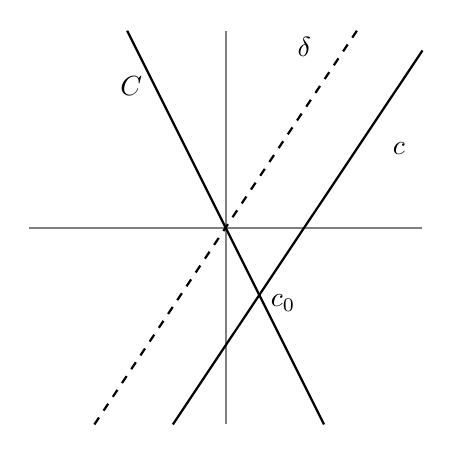
\begin{tikzpicture}
            % Draw axes
            \draw[gray, thick] (-2.5,0) -- (2.5,0);
            \draw[gray, thick] (0,-2.5) -- (0,2.5);
            
            % Line C: passes through origin with slope -2
            \draw[thick] (-1.25,2.5) -- (1.25,-2.5);
            \node at (-1.2,1.8) {$C$};
            
            % Line im(delta): dashed, passes through origin with slope 1.5
            \draw[thick, dashed] ({-2.5/1.5},-2.5) -- ({2.5/1.5},2.5);
            \node at (1,2.3) {$\im \delta$};
            
            % Line im(c): parallel to im(delta), equation y = 1.5x - 1.5
            \draw[thick] (-0.67,-2.5) -- (2.5,{1.5*2.5-1.5});
            \node at (2.2,1.0) {$\im c$};
            \node at ({3/7 + 0.3},{-6/7 - 0.1}) {$c_0$};
        \end{tikzpicture} 
    \end{center}
    \caption{The values of the (representative of the) structure function $c$ inside $\Hom(V\wedge V,V)$ span an affine subspace modeled on $\im\delta$, and any complement $C$ is (non-canonically) isomorphic to $\coker\delta$. A choice of $C$ is equivalent to a choice of a $c_0\in \im c$. Conversely, if $C$ is chosen, $c_0$ can be identified with the equivalence class $[c]=\im c=c+\im \delta$. \label{fig: imc in hom(vv,v)}}
\end{figure}
           
\begin{rem}
    Since the fibers of $\rmJ^1 P$ are only affine spaces, the image of $c$ inside $\Hom(V\wedge V,V)$ is generally an \emph{affine subspace}, not a vector subspace, see Figure~\ref{fig: imc in hom(vv,v)}. As we have just established, it is modeled on the vector space $\im\delta$. Despite it being an affine space, the quotient $\Hom(V\wedge V,V)\slash \im c$ is still well-defined and is also an affine space, modeled on $\coker\delta$. If we identify $\coker\delta$ with some arbitrarily chosen complement $C$ of $\im\delta$ such that $\Hom(V\wedge V,V)=\im\delta\oplus C$, then we can visualize $c$ as taking values in the affine plane $c_0+\im\delta$, where $\{c_0\}=C\cap \im c$. Thus, $C\cong \coker\delta$ is the ``space of possible offsets'' of the space of torsions away from the origin. The $G$-structure is characterized, to first order, by the value of these offset at each point, i.e., $[c]$, which can also be called the ``irreducible part'' of the torsion.
\end{rem}

Next we can see how $[c]$ varies along the fibers of $P$. The following is a simple exercise.

\begin{prop}[{\cite[p.~318]{Sternberg}}]
    The structure function is equivariant under the principal $G$-action:
    \[c_{\Phi_{g\ast}(\calH)}=\sigma_g^{-1}c_\calH,\]
    where $\sigma$ is the standard induced action $G\acts \Hom(V\wedge V,V)$ given by $(\sigma_g \beta)(u\wedge v)=g\cdot \beta(g^{-1}\cdot u\wedge g^{-1}\cdot v)$.
\end{prop}

The reader can also easily check that the space $\im\delta$ is a $G$-invariant subspace of $\Hom(V\wedge V,V)$. Therefore, the quotient space $\coker\delta$ still carries a $G$-representation which we also denote by $\sigma$. In summary, we have 
\[[c](p\cdot g)=\sigma_g^{-1}[c](p).\]

\begin{rem}
    Recall that equivariant functions on a principal bundle correspond to sections of the associated bundle. In this case, since $V$ is the model tangent space of $M$, the associated bundle with fiber $\Hom(V\wedge V,V)$ is literally the bundle of $\T M$-valued $2$-forms on $M$. Thus, $c$ can be identified with a tensor field of type $(1,2)$ on $M$, called the \emph{torsion tensor}, and upon a choice of complement $C\cong \coker\delta$, the part $c_0$ of this tensor belonging to $C$ is the \emph{intrinsic torsion tensor}. One has to be careful, however, to always specify the choice of $C$ because, depending on that choice, $c_0$ can be any point of $\im c$.
\end{rem}

Finally, since the structure function is clearly a natural (intrinsic) quantity of the $G$-structure, equivalent $G$-structures have equivalent structure functions.

\begin{prop}[{\cite[Thm.~VII.2.1]{Sternberg}}]\label{thm vii.2.1 Sternberg}
    If $F:M\to \wb M$ is a local diffeomorphism establishing an equivalence of two $G$-structures $P\to M$ and $\wb P\to \wb M$, then the structure functions are also $F$-related: $[c]=[\wb c]\circ F_\ast$.
\end{prop}

In particular, we immediately get

\begin{cor}[{\cite[Thm.~VII.2.2]{Sternberg}}]\label{thm vii.2.2 Sternberg}
    If a $G$-structure is locally flat, then its structure function vanishes identically.
\end{cor}
\begin{proof}
    We need to show that the structure function of the standard flat $G$-structre $P=V\times G$ is zero. It suffices to find \emph{any} horizontal subspace $\calH$ at, say, $p=(0,e)$, such that $c_\calH=0$. Naturally, we let $\calH$ be tangent to the horizontal slice $P_{\{e\}}=V\times \{e\}$, which is in fact an $\{e\}$-substructure, namely the canonical absolute parallelism on $V$. It now suffices to show that $\dd\theta$ vanishes identically on the canonical absolute parallelism of $V$. Since the group is $\{e\}$, the projection $\pi:P_{\{e\}}\to V$ is a diffeomorphism. Then $(\pi^{-1})^\ast \theta$ is a form on $V$. By definition, $(\pi^{-1})^\ast\theta=\dd \id_V$. Therefore, $\dd\theta=0$.
\end{proof}

The converse is not true in general. In fact, as we will see, for many important groups $G$, the first-order structure function vanishes \emph{regardless} of the $G$-structure $P$. When this happens, the first-order structure function gives no information and we must look for higher-order invariants.

The converse of Corollary~\ref{thm vii.2.2 Sternberg} is true for \emph{some} groups, however, and we now give some examples.

\begin{rem}\label{rem p320 Sternberg}
    Suppose $G$ leaves invariant a subspace $V_1<V$. There is an obvious projection $\tau:\Hom(V\wedge V,V)\to \Hom(V_1\wedge V_1,V\slash V_1)$, namely, for $t\in \Hom(V\wedge V,V)$ and $v_1,v_2\in V_1$, we put \[\tau(t)(v_1\wedge v_2)\coloneqq t(v_1\wedge v_2)+V_1.\] 
    Then 
    \[\ker\tau=\{t\in\Hom(V\wedge V,V)\mid t(V_1\wedge V_1)\subset V_1\}.\]
    Now, if $\frakg$ leaves $V_1$ invariant, $\frakg\cdot V_1<V_1$, then for any $f\in \Lin(V,\frakg)$,
    \[\delta(f)(V_1\wedge V_1)=f(V_1)\cdot V_1-f(V_1)\cdot V_1\quad < \quad V_1.\]
    Thus, $\delta(f)\in \ker\tau$. We therefore have a quotient map
    \[\eta:\coker\delta\to \Hom(V_1\wedge V_1,V\slash V_1),\]
    and so $\eta\circ c:P\to \Hom(V_1\wedge V_1,V\slash V_1)$.
\end{rem}

\begin{example}[Intrinsic torsion of a distribution]
    Suppose $V_1<V$ is a $k$-dimensional subspace and $G<\GL(V)$ is the group of \emph{all} linear transformations leaving $V_1$ invariant, $G\cdot V_1<V_1$. One can immediately notice that that $G$ has exactly the structure of the group in Example~\ref{ex foliation g-structure}, so a $G$-structure is the same as a rank $k$ distribution on $M$. Let us also give an explicit proof of this correspondence. Consider a $G$-structure $P\overset{\pi}{\to} M$, viewed as a subbundle of the frame bundle $\Fr(\T M)$. Let $p\in P$ and $m=\pi (P)$. Define the subspace $D_m<\T_m M$ by $D_m=p(V_1)$, where $p$ is interpreted as a frame, i.e., a linear isomorphism $V\to \T_m M$. For any $g\in G$, we have $(p\cdot g)(V_1)=p(g\cdot V_1)=p(V_1)$, so $D_m$ doesn't depend of the choice of $p\in P_m$. Thus, $P$ determines a rank $k$ distribution on $M$. Conversely, let $D$ be a  rank $k$ distribution on $M$ and let $P$ be the submanifold of $\Fr(\T M)$ consisting of those frames $p$ with $p^{-1}(D_m)=V_1$, where $m=\pi(p)$. Then $P$ is easily seen to be a $G$-structure.

    Now, it is easy to check that for this $G$, in terms of Remark~\ref{rem p320 Sternberg}, $\im\delta=\ker\tau$, so $\eta$ is an isomorphism. But the vanishing of $\eta\circ c$ is \emph{precisely} the statement of involutivity of the distribution $D$, so by the Frobenius Theorem, $D$ is integrable in this case, and $P$ is locally flat. So for this group $G$, the converse of Corollary~\ref{thm vii.2.2 Sternberg} holds.
\end{example}

\begin{example}[Intrinsic torsion of an almost symplectic structure]
    Let $P\to M$ be an almost symplectic structure given by an almost symplectic form $\omega\in\Omega^2(M)$ (so $\dim M=n$ is even). We will now show that the first-order structure function on $P$ vanishes iff $\dd\omega=0$. First recall that the soldering form $\theta_p$ on the frame bundle $\Fr(\T M)$ is defined as $p^{-1}\circ \pi_\ast$, where $p\in P\subset \Fr(\T^\ast M)$ is treated as a linear isomorphism $p:V\to \T_m M$. Since $P$ is an almost symplectic structure, $p$ is actually an isomorphism of symplectic vector spaces, where $V$ carries a standard symplectic structure, which we denote by $\omega_0$, and $\T_m M$ carries $\omega_m$. Thus, letting $\calH$ be a horizontal space at $p\in P_m$,
    \[c_\calH(u,v)=\dd\theta_p(p(u)^h_p,p(v)^h_p),\quad u,v,\in V,\] 
    where $X^h_p$ for any $X\in \T_m M$ denotes the unique horizontal vector in $\calH$ such that $\pi_\ast(X^h_p)=X$. 

    The intrinsic torsion of a $G$-structure is a section of a bundle associated to the frame bundle with fiber $\coker\delta$, and therefore, can \emph{always} be represented by a tensor, provided some convenient choice of complement to $\im\delta$  inside the space of vector-valued $2$-forms $\Hom(V\wedge V,V)$. Thus, the identification of $c$ as a tensor typically proceeds in two steps. First, an algebraic step where $\ker\delta$ and $\coker\delta$ are computed. The second step is the construction of a natural tensor field on $M$ that takes values in the subbundle correponding to $\coker\delta$. 

    We begin by describing the Spencer differential \[\delta:V^\ast\otimes\fraksp(V)\to V^\ast\wedge V^\ast\otimes V.\]
    Here, $\fraksp(V)$ is the Lie algebra of the group of symplectomorphisms of $(V,\omega_0)$ (its elements are called \emph{Hamiltonian matrices}). Thus, we have the inclusion $\fraksp(V)<\frakgl(V)=V^\ast\otimes V$, and $\delta$ acts by antisymmetrizing over the two $V^\ast$ factors. Note that $\dim \fraksp(V)=n(n+1)/2$, which is also the dimensionality of the space of symmetric matrices on $V$. In fact, there is a natural isomorphism 
    \[\psi:V\odot V\to \fraksp(V),\quad \psi(v\odot w)\cdot u=\omega_0(v,u)w+\omega_0(w,u)v.\]
    In simpler terms, using the symplectic form to lower one index on a symmetric bivector gives a Hamiltonian matrix. In even simpler terms, $\rmJ\cdot S$ is Hamiltonian for any symmetric matrix $S$, where $\rmJ$ is the matrix representing $\omega_0$. With this isomorphism, and also by using $\omega_0$ as an isomorphism $V\to V^\ast$, the Spencer differential becomes 
    \[\delta:V\otimes V\odot V\to V\wedge V \otimes V.\]
    Now, since $\delta$ merely antisymmetrizes over the first two components, it becomes obvious that $\ker\delta\cong V\odot V\odot V$ and $\im\delta=V\wedge V\odot V$. We end up with a very convenient representation for the cokernel: 
    \[\coker\delta\cong (V\wedge V\otimes V)\slash \im V\cong V\wedge V\wedge V,\] 
    so the exact Spencer sequence reads
    \[0\to V\odot V\odot V\to V\otimes V\odot V \to V\wedge V\otimes V\to V\wedge V\wedge V\to 0.\]

    Thus, intrinsic torsion will be identified with a differential $3$-form on $M$. To identify this form, we can act with the intrisic torsion on an arbitrary collection of vector fields. Suppose $u,v,w\in V$ and we pick a smooth horizontal distribution $\calH P$ locally around $p\in P$. Then there are local horizontal vector fields $X^h$, $Y^h$, $Z^h$ around $p$, uniquely defined by taking values in $\calH P$ and satisfying $\theta(X^h)=u$, $\theta(Y^h)=v$, $\theta(Z^h)=w$. Using the standard formula \eqref{eq prop 4.1.6} for the exterior derivative of a $1$-form, we have
    \[\dd\theta(X^h,Y^h)=-\theta([X^h,Y^h]).\]
    To construct the necessary $3$-form as above, we need to apply $\omega_0$ to this vector together with $\theta(Z^h)$ and then antisymmetrize. By construction, $\theta$ identifies the symplectic structure of $\T M$ (lifted to each horizontal space) with the symplectic structure of $V$, thus,
    \[\omega_0(-\theta([X^h,Y^h]),\theta(Z^h))=(\pi^\ast\omega)(-[X^h,Y^h],Z^h).\]
    But since $(\pi^\ast\omega)(X_1^h,X_2^h)=\omega_0(u_1,u_2)$ for any pair of horizontal vector fields as above, we once again use the general formula \eqref{eq d in terms of Lie} for the exterior derivative of a $2$-form to see that the antisymmetrization of $(\pi^\ast\omega)(-[X^h,Y^h],Z^h)$ gives, up to some unimportant normalization factor depending on the definition of ``antisymmetrization'', exactly 
    \[\dd (\pi^\ast\omega)_p(X^h,Y^h,Z^h)=(\pi^\ast\dd\omega)_p(X^h,Y^h,Z^h)=\dd\omega(p(u),p(v),p(w)).\]

    Lastly, the Darboux Theorem implies the converse of Corollary~\ref{thm vii.2.2 Sternberg} for almost symplectic structures. In other words, \emph{torsion-free almost symplectic structures are integrable}, and are called \emph{symplectic structures}.
\end{example}


\begin{rem}
    The above example becomes much more straightfoward if one allows the usage of affine connections. With an affine connection $\nabla$ on $\T M$, one has the general identity
    \[\dd\omega (\_,\_,\_)=\cyclic \left[\nabla_{\_}\omega(\_,\_)+\omega\left(\sfT^\nabla(\_,\_),\_\right)\right],\]
    where $\cyclic$ is the sum over the $3$ cyclic permutations of the arguments and $\sfT^\nabla\in\Gamma^1_2(M)$ is the torsion tensor of the connection. Then it is easy to show that $\nabla$ can be chosen so as to be \emph{almost symplectic} (i.e., $\nabla\omega=0$) and so that $\omega\left(\sfT^\nabla(\_,\_),\_\right)=\frac13\dd\omega(\_,\_,\_)$, see \cite[Thm.~2.1]{Albuquerque2015}. Combined with the above argument computing $\coker\delta$, this once again identifies the intrinsic torsion of the $G$-structure with $\dd\omega$ by explicitly constructing a connection (i.e., a choice of horizontal distribution $\calH P$) such that the torsion tensor takes values in the subbundle corresponding to $\coker\delta$.
\end{rem}

Indeed, in the context of equivalence problems, affine connections, despite not being intrinsic to the problems themselves, turn out to be an essential tool that allows one to reduce complex questions like that in the above example to straightforward and universal algebraic algorithms. Hence, the reader should not feel discouraged by the complexity of the above arguments. The following \chap\ will be devoted to Cartan's systematic algebraic approach for finding the differential invariants intrinsic to \emph{any} system of differential equations, including ones describing equivalences of $G$-structures.

\begin{example}[Complex structures]
    A final classical example where the converse to Corollary~\ref{thm vii.2.2 Sternberg} holds is the case of almost complex ($\GL_n(\bbC)$-) structures. The first-order structure function of such a structure is called the \emph{Nijenhuis tensor}, and the Newlander-Nirenberg Theorem \index{Theorem!Newlander-Nirenberg} shows that its vanishing is equivalent to the integrability of the structure, i.e., to the existence of a corresponding complex-analytic atlas on $M$. The proof relies heavily on functional analysis, but if one assumes that the structure is real-analytic, there is a relatively simple geometric proof which we will provide later.
\end{example}

\begin{rem}
    Torsion-free $G$-structures are not the only distinguished structures. If $\coker\delta$ is not an irreducible representation of $G$, then it decomposes into a direct sum of irreducible components. One may then define special subclasses of $G$-structures whose intrinsic torsion takes values only in one of these irreducible components. In Riemannian geometry, intrinsic torsion is always zero, but the second-order structure function (related to curvature) is not, and the classification of Riemannian geometries based on the representation of $\frakso_n$ in which the second-order structure function takes values was a major problem in geometry in the 20-th century, solved by Marcel Berger, Jim Simons, Robert Bryant, and others.
\end{rem}






\section{Cartan's equivalence method}\label{sec: cartan equiv method}


Let us return to the general equivalence problem for $G$-structures. Theorem~\ref{thm vii.2.1 Sternberg} asserts that if we want to find an isomorphism between two $G$-structures $P$ and $\wb P$, then we must \emph{at least} be able to find a map $F_\ast:P\to \wb P$ such that $F^\ast [\wb c]=[c]$. In general, this kind of problem is very difficult. The one easy case is where one of the functions is constant. Then the other structure function must also be equal to the same constant. 

\begin{cor}[{\cite[Cor.~VII.2.1]{Sternberg}}]\label{cor vii.2.1 Sternberg}
    Let $P$ be a $G$-structure with a constant structure function. Any $G$-structure locally equivalent to $P$ must have the same constant as its structure function.
\end{cor}

In general, we have to resort to the method of classifying spaces, as in \S\ref{sec: equiv of coframes}, to establish equivalence. In any case, the first-order structure function typically does not suffice. We continue by constructing the second-order structure function.

Recall that the affine bundle $\pi^1_0:\rmJ^1 \Fr(\T M)\to \Fr(\T M)$ can be identified with a subbundle of the second frame bundle $\Fr(\T \Fr(M))\cong\Fr^2(M)$, and thus can be interpreted as a $\Hom(V,\frakgl(V))$-structure on the manifold $\Fr(M)$, where we view the vector group $\Hom(V,\frakgl(V))<\GL(V\oplus\frakgl(V))$ (where $V\oplus\frakgl(V)$ serves as the model tangent space of $\Fr(M)$) as the subgroup formed by the ``vertical shifts''
\[(v,A)\mapsto (v,A+\omega(v)),\quad \omega\in \Hom(V,\frakgl(V)).\]

Thus, by the same argument, any first-order $G$-structure $P\subset \Fr(M)$ on $M$ also gives rise to an interpretation of the affine bundle $\pi^1_0:\rmJ^1 P\to P$ as a $\Hom(V,\frakg)$-structure on $P$.


\begin{example}
    Consider the standard flat $G$-structure on $\bbR^n$:
    \[P\coloneqq \bbR^n\times G<\Fr(\bbR^n)=\bbR^n\times\GL_n(\bbR).\]
    Given a vector field $X\in\fX(\bbR^n)=C^\infty(\bbR^n,\bbR^n)$, we can observe that $X$ is an infinitesimal automorphism of $P$ iff its flow $\Fl^X_t$ lifts to an automorphism $(\Fl^X_t)_\ast:P\to P$. The lifted flow is the flow of a lifted vector field $\wt X\in\fX(P)$: in coordinates $\bf x$, so that $X=X^i\partial_i$, the lifted vector field is 
    \[\wt X=\frac{\partial X^i}{\partial x^j}\frac{\partial}{\partial p^i_j},\]
    where $p^i_j$ are the associated coordinates on $\Fr(\bbR^n)$ so that a frame $p\in \Fr(\bbR^n)$ is written as the collection of $n$ tangent vectors
    \[p=\left(p^i_1\partial_i,\ldots,p^i_n\partial_i\right).\]
    It follows that $X$ is an infinitesimal automorphism iff 
    \[\left[\frac{\partial X^i}{\partial x^j}\right]_{i,j=1,\ldots,n}\in\frakg <\frakgl_n(\bbR),\]
    i.e., iff the Jacobi matrix of the flow of $X$ at every point belongs to $G$. Let us assume now that the lifted flow fixes the basepoint $(0,e)\in \bbR^n\times\GL_n(\bbR)$. The lifted vector field $\wt X$ vanishes at this point. If we now prolong to the jet bundle $\rmJ^1 P$, we obtain a flow which is generated by the vector field 
    \[\rmj^1\wt X=\frac{\partial X^i}{\partial x^{j_1}\partial x^{j_2}}\frac{\partial}{\partial p^i_{j_1,j_2}}\eqqcolon \wt X^i_{j_1,j_2}\frac{\partial}{\partial p^i_{j_1,j_2}},\]
    where $(x^i,p^i_j,p^i_{j_1,j_2})$ are the canonical coordinates on the jet bundle. Note that the components $\wt X^i_{j_1,j_2}$ satisfy 
    \[\left[\wt X^i_{j_1,j_2}\right]_{i,j_1=1,\ldots,n}\in\frakg<\frakgl_n(\bbR),\quad j_2=1,\ldots,n,\]
    and are symmetric in the lower indices $j_1,j_2$. We conclude that:
    \begin{lem}
        The lifts of the infinitesimal automorphisms of the standard flat $G$-structure $P=V\times G$ to the jet space $\rmJ^1 P$ generate a Lie subgroup $G^{(1)}<\Hom(V,\frakg)$ with Lie algebra\footnote{Readers familiar with the theory of connections may recognize this as the torsion-free condition for $G$-connections $\omega$, akin to the symmetry of the Christoffel symbols in Riemannian geometry. More precisely, however, it is the \emph{first-order compatibility condition}. The $0$-th order compatibility condition simply requires the connection to be $\frakg$-valued, whereas $\frakg^{(1)}$-valuedness means that the connection is a section of $P^{(1)}$ rather than just $\rmJ^1 P$. As we will see, $\frakg^{(1)}$ is the model for the affine space of connections with a given value of torsion, so in particular, if we want no torsion, the connection must be $P^{(1)}$-valued. On the other hand, the \emph{existence} question of whether vanishing torsion is actually attainable will be answered later in this \sect.}
        \[\frakg^{(1)}\coloneqq \ker\delta=\{\omega\in\Hom(V,\frakg):\omega(u)v=\omega(v)u\;\text{ for all }u,v\in V\},\]
        where $\delta$ is the Spencer antisymmetrization operator from \eqref{eq spencer kernel-cokernel seq}.
    \end{lem}
\end{example}

The above example motivates the following definition.

\begin{defn}[Prolongation of a Lie algebra]\index{Prolongation!of Lie algebras}
    Let $\frakg<\frakgl(V)$ be a matrix Lie algebra (here, $V$ is a finite-dimensional vector space). The first prolongation of $\frakg$ is the subspace $\frakg^{(1)}<\Hom(V,\frakg)$ defined by
    \[\frakg^{(1)}\coloneqq \ker\delta=\{\omega\in\Hom(V,\frakg):\omega(u)v=\omega(v)u\;\text{ for all }u,v\in V\}.\]
    It is a Lie algebra by virtue of the faithful matrix representation 
    \[\frakg^{(1)}\acts(V\oplus\frakg): \quad \omega^1\cdot (v,A)\coloneqq (0,\omega(v)),\quad \omega\in \frakg^{(1)}<\Hom(V,\frakg),\]
    which can also be written as a block matrix 
    \[\begin{pmatrix}
        0 & 0 \\
        \omega & 0
    \end{pmatrix}\in\End(V\oplus \frakg).\label{eq g(1) action}\]
    This identifies $\frakg^{(1)}$ with a Lie subalgebra of $\frakgl(V\oplus\frakg)$, allowing us to iterate the definition. The $r$-th prolongation of $\frakg$ is the subspace 
    \[\frakg^{(r)}<\Hom(V\oplus\frakg\oplus\cdots\oplus \frakg^{(r-2)},\frakg^{(r-1)}),\] defined inductively by 
    \[\frakg^{(k)}=\left(\frakg^{(r-1)}\right)^{(1)}, \quad\quad \frakg^{(-1)}\coloneqq V,\;\frakg^{(0)}\coloneqq \frakg.\]
    A Lie algebra $\frakg$ is said to be of \emph{finite type $r\geq 1$} if  $\frakg^{(r-1)}\neq 0$ and $\frakg^{(r)}=0$.
\end{defn}

Importantly, prolongations are \emph{not intrinsic} to the Lie algebra $\frakg$. Even under the above assumption that the representation $\frakg\acts V$ is faithful, different representations can produce different prolongations.

\begin{xca}
    Consider $\frakg=\bbR$ and $V=\bbR^2$, but one action by scalings $(x,y)\mapsto (tx,ty)$, and another one by shears $(x,y)\mapsto (ty,0)$. Show that $\frakg^{(1)}=0$ in the former case and $\frakg^{(1)}\cong \bbR$ in the latter.
\end{xca}

In addition, without explaining the notation for now, we name the important space $\coker\delta$:
\[\rmH^{0,2}(\frakg)\coloneqq \coker\delta=\frac{\Hom(V\wedge V,V)}{\delta\left(\Hom(V,\frakg)\right)},\]
which lets us rewrite the kernel-cokernel sequence \eqref{eq spencer kernel-cokernel seq} as 
\[0\to \frakg^{(1)}\to \Hom(V,\frakg)\overset{\delta}{\to}\Hom(V\wedge V,V)\to \rmH^{0,2}(\frakg)\to 0. \]

\begin{example}[$\frakso_n^{(1)}$ and $\rmH^{(0,2)}(\frakso_n)$]\label{ex so(n) prolongation}
    Consider $G=\SO_n<\GL_n(\bbR)$, which is the setting of Riemannian geometry. Since such a structure is equivalent to a Riemannian metric $\sfg$ on $M$, which is modeled on a fixed inner product on $V$, we can use this inner product to identify $V$ with $V^\ast$. Under this identification, the algebra $\frakso_n$ becomes the space $\bigwedge^2 V$ of $2$-forms. Now, $\frakso_n^{(1)}=\left(\bigwedge^2 V^\ast\otimes V^\ast\right)\cap \left(V^\ast\otimes \bigodot^2 V^\ast\right)$. An element $A_{ijk}\dd x^i\otimes \dd x^j\otimes \dd x^k$ of this space is antisymmetric in the first two indices and symmetric in the last two, so
    \[A_{ijk}=-A_{jik}=-A_{jki}=A_{kji}=A_{kij}=-A_{ikj}=-A_{ijk}.\]
    Thus, $\frakso_n^{(1)}=0$. 
    
    Furthermore, since $\frakso_n^{(1)}=\ker\delta$, this implies that 
    \[\dim\im \delta=\dim \Hom(V,\frakso_n)=\dim \Hom(V,V\wedge V)=\dim \Hom(V\wedge V,V),\]
    which implies $\rmH^{(0,2)}=0$.
\end{example}

\begin{example}[$\frakco_n^{(1)}$]\label{ex co(1)}
    Now consider the conformal algebra $\frakco(V)\cong \frakso(V)\oplus\bbR$. It consists of all $A\in\frakgl(V)$ satisfying 
    \[\<Au,v\>+\<u,Av\> = \lambda_A \<u,v\>,\]
    where $\<\,,\,\>$ is a fixed inner product on $V$ and $\lambda_A\in\bbR$ (depending linearly on $A$). Let $\omega\in \frakco_n^{(1)}<\Hom(V,\frakg)$ and consider the $1$-form 
    \[\alpha_\omega \in V^\ast:\quad \alpha_\omega(u)=\lambda_{\omega(u)}.\]
    The map $\omega\mapsto \alpha_\omega$ is clearly injective: if $\omega$ is in its kernel, then $\omega\in\frakso_n^{(1)}$, which vanishes by the preceding example. Let us show that it is also surjective. To this effect, observe that $\<\,,\,\>$ induces an isomorphism of $V$ onto $V^\ast$. Thus, $u\in V$ is mapped to $u^\flat\in  V^\ast$ defined by $u^\flat(v)=\<u,v\>$. If we replace $\<\,,\,\>$ by $\lambda\<\,,\,\>$, then under the new isomorphism $u$ gets sent to $\lambda u^\flat$. In particular, the isomorphism of $\phi:V\otimes V^\ast\to V^\ast\otimes V$ induced by $\<\,,\,\>$ is independent of the scalar $\lambda$, i.e., is an invariant of $\frakco(V)$. Let us denote this isomorphism by $\phi$. For any $\alpha\in V^\ast$ let $\gamma(\alpha)\in \Hom(V,\Hom(V,V))$ be defined by 
    \[\gamma(\alpha)(v)=v\otimes \alpha-\phi(\alpha\otimes v)+\alpha(v)\id_V.\]
    We claim that $\gamma(\alpha)\in\frakso(V)^{(1)}$. In fact, 
    \[\gamma(\alpha)(v_1)\cdot v_2 = \alpha(v_1)v_2 + \alpha(v_2)v_1-\<v_1,v_2\>u\]
    is clearly symmetric in $v_1,v_2$. Furthermore, 
    \[\<\gamma(\alpha)(v_1)v_2,v_3\>+\<v_2,\gamma(\alpha)(v_1)v_3\>=2\alpha(v_1)\<v_2,v_3\>.\]
    This proves that $\gamma(\alpha)\in\frakco(V)^{(1)}$, and it is also easy to check that it is the inverse of $\omega\mapsto \alpha_\omega$. We conclude that $\frakco(V)^{(1)}\cong V^\ast$.
\end{example}

\begin{defn}[Prolongation of a Lie group]\index{Prolongation!of Lie groups}
    Let $G<\GL(V)$ be a matrix Lie group. The first prolongation of $G$ is the subgroup $G^{(1)}<\GL(V\oplus\frakg)$ consisting of transformations of the form 
    \[(v,A)\mapsto (v,A+\omega(v)),\quad \omega\in\frakg^{(1)}.\]
    Similarly, the $r$-th prolongation of $G$ is the subgroup $G^{(r)}<\GL(V\oplus \frakg\oplus \frakg^{(1)}\oplus\cdots\oplus \frakg^{(r)})$ defined inductively by 
    \[G^{(r)}\coloneqq \left(G^{(r-1)}\right)^{(1)}.\]
\end{defn}

Thus, $G^{(1)}$ is faithfully represented on $V\oplus\frakg$ by block matrices of the form 
\[\begin{pmatrix}
    \id_V & 0 \\
    \omega & \id_\frakg
\end{pmatrix}\in\End(V\oplus \frakg),\quad\quad  \omega\in\frakg^{(1)}<\Hom(V,\frakg).\label{eq G(1) action}\]
Note that all prolongations $G^{(r)}$ are abelian groups. Now, for each $G$-structure $P\to M$ we can always reduce the structure group of $\rmJ^1 P$ to $G^{(1)}$, obtaining a $G^{(1)}$-structure.

\begin{prop}[{\cite[Prop.~2.11]{Fernandes}}]
    Let $P\to M$ be a $G$-structure on $M$ with (pre-quotient) first-order structure function $c:\rmJ^1 P\to \Hom(V\wedge V,V)$. Each choice of complement $C$ to $\im\delta$ in $\Hom(V\wedge V,V)$ (so $\Hom(V\wedge V,V)=\im\delta\oplus C$) determines a smooth subbundle 
    \[P^{(1)}\coloneqq \{\calH\in \rmJ^1 P:c_{\calH}\in C\}=c^{-1}(C)<\rmJ^1 P,\]
    which is a reduction of the affine bundle $\pi^1_0:\rmJ^1 P\to P$ to the structure group $G^{(1)}$. Different choices of $C$ determine subbundles related via a principal right translation by an element in $\Hom(V,\frakg)$.
\end{prop}

The $G^{(1)}$-structure $P^{(1)}\to P$ is called the \emph{first prolongation} of $P$. Of course, working inductively, one defines the $r$-th prolongation:\index{Prolongation!of $G$-structures}
\[P^{(r)}\coloneqq \left(P^{(r-1)}\right)^{(1)}<\rmJ^r P<\Fr^r(M),\]
which is a $G^{(r)}$-structure on the manifold $P^{(r-1)}$. The relevance of the prolongation to the equivalence problem is explained by the following basic result.

\begin{thm}[{\cite[Prop.~2.12]{Fernandes},\cite[Thm.~VII.3.2]{Sternberg}}]\label{thm 2.12 Fernandes}
    Let $P\to M$ and $\wb P\to \wb M$ be $G$-structures. They are equivalent iff their first prolongations $P^{(1)}\to P$ and $\wb P^{(1)}\to \wb P$ are equivalent as $G^{(1)}$-structures (assuming identical choice of complement $C$).
\end{thm}

We can use this to obtain genuinely new necessary conditions for equivalence (so far we only have $c$) by looking at the structure function of the prolongation $P^{(1)}$:
\[[c^{(1)}]:P^{(1)}\to \frac{\Hom\left(\bigwedge^2(V\oplus\frakg),V\oplus \frakg\right)}{\delta(\Hom(V\oplus\frakg,\frakg^{(1)}))},\]
called the \emph{second-order structure function of $P$}. Then one continues this process by constructing higher and higher prolongations and analyzing their structure functions. The importance of structures of finite type is that we can reduce the set of necessary conditions for equivalence of $G$-structures to a finite amount. In fact, by the method of prolongation, the equivalence problem for finite type $G$-structures reduces to an equivalence problem for $\{e\}$-structures (coframes), since $G^{(r)}=\{e\}$ for some $r$, which we already know how to solve. Moreover, one can show that $G$-structures of finite type always have finite-dimensional symmetry groups (this will follow from the rigidity result for general Cartan geometries, of which any $\{e\}$-structure is a trivial example, see Theorem~\ref{thm 1.5.11 Cap}).

\begin{rem}
    As we will see, an $\{e\}$-structure, also known as an absolute parallelism, defines a unique connection. Thus, for finite-type $G$-structures our method guarantees the construction of a canonical affine connection on $P^{(r-1)}$, which is a specific type of Cartan geometry. In other words, finite type $G$-structures end up being special Cartan geometries, and by virtue of Theorem~\ref{thm 2.12 Fernandes} their equivalence can be established using the general procedure for the equivalence of coframes. For an explicit description of the canonical Cartan geometry associated with a $G$-structure of type $2$ see \cite{Alekseevsky}. We treat the case of type $1$ next.
\end{rem}

The function $c^{(1)}$ always contains certain components that carry no information, so we will now examine its decomposition. Let $p'=\calH_p\in P^{(1)}$ and let $p''=\calH_{p'}$ be a horizontal subspace of $\T_{p'} P^{(1)}$ (horizontal w.r.t.\ $\pi^1_0:P^{(1)}\to P$). Then $c_{p''}^{(1)}\in \Hom\left(\bigwedge^2(V\oplus\frakg),V\oplus\frakg\right)$ can be naturally decomposed into three components:
\begin{multline}
    \Hom\left(\bigwedge^2(V\oplus\frakg),V\oplus\frakg\right)\cong \\
    \cong \Hom\left(V\wedge V,V\oplus\frakg\right)\oplus \Hom\left(V\otimes\frakg,V\oplus\frakg\right)^2_{\mathrm{asym}}\oplus\Hom\left(\frakg\wedge\frakg,V\oplus\frakg\right).
\end{multline}
(There are two copies of $\Hom\left(V\otimes\frakg,V\oplus\frakg\right)$ and we antisymmetrize them at the end.) Let us describe each of the components of the (representative of the) second-order structure function. We fix $u,v\in V$ and $A,B\in\frakg$:
\begin{enumerate}
    \item The first component of $c_{p''}^{(1)}$ further decomposes into a $V$-valued and a $\frakg$-valued component, the first one being the (lift of the) first-order structure function of $P$:
    \[u\wedge v\mapsto c_{p'}(u,v)\oplus\rho_{p''}(u,v),\quad \rho_{p''}\in\Hom(V\wedge V,\frakg).\]
    \item The $\Hom\left(V\otimes\frakg,V\oplus\frakg\right)$ component of $c_{p''}^{(1)}$ is similarly decomposed into a $V$-valued and a $\frakg$-valued component:
    \[(u,A)\mapsto -A\cdot u\oplus S_{p''}(A,u),\quad S_{p''}\in\Hom(\frakg\otimes V,\frakg).\]
    The first term is fixed because $\theta$ is equivariant, $\Lie_{A_\ast}\theta=-A\cdot\theta$, cf.~\eqref{eq vii.2.5 Sternberg}.
    \item The last component of $c_{p''}^{(1)}$ must be purely $\frakg$-valued and is simply the Lie bracket:
    \[A\wedge B\mapsto -[A,B],\]
    corresponding to the Lie bracket of Killing vector fields: $[A_\ast,B_\ast]=-[A,B]_\ast$.
\end{enumerate}
Thus, in total, we have 
\begin{multline}
    c_{p''}^{(1)}(u,A,v,B)=\left(c_{p'}(u,v)-A\cdot u+B\cdot v\right)\oplus\\\oplus\left(\rho_{p''}(u,v)+S_{p''}(A,u)-S_{p''}(B,v)-[A,B]\right).
\end{multline}
Thus, only $\rho_{p''}$ and $S_{p''}$ contain any new (second-order) differential invariants. 


\begin{rem}[$G$-structures of type $1$]\label{rem g-structures of type 1}
    An important special case occurs when $G^{(1)}=\{e\}$ (for instance, in Riemannian geometry, where $G=\SO_n$). In this case, $P^{(1)}$ is an $\{e\}$-structure, i.e., a global coframe on $P$, and $\pi^1_0:P^{(1)}\to P$ is a diffeomorphism, which therefore prescribes a unique horizontal space $\calH_p$ at each $p\in P$ by virtue of $p''=\calH_{p'}=\calV_pP\oplus (\pi^1_0)^\ast \calH_p$. In other words, every $G$-structure of finite type $1$ carries a \emph{canonical pseudoconnection} $\omega\in\Omega^1(P,\frakg)$. The pair $(\theta,\omega)$ is the corresponding global coframe on $P$. Since $P^{(1)}\cong P$, we may view the second-order function as a function on $P$. Upon doing so, the above decompositions are equivalent to the following form of the structure equations for the coframe $(\theta,\omega)$ in terms of $c,\rho$, and $S$:
    \[
    \begin{aligned}
        \dd\theta & = c\circ \theta\wedge\theta-\omega\wedge\theta,\\
        \dd\omega & = \rho\circ \theta\wedge\theta+S\circ \omega\wedge\theta-\omega\wedge\omega,
    \end{aligned}
    \]
    where $\omega\wedge\theta$ is the $V$-valued $2$-form obtained from the $\frakg$-action on $V$ and $\omega\wedge\omega=\frac12[\omega,\omega]$. Note that the first equation is the $V$-valued component and involves only first-order structure functions, whereas the second is the $\frakg$-valued component and involves only second-order structure functions. Had we not assumed that $G^{(1)}=\{e\}$, we would have also had $\frakg^{(r)}$-valued components of the coframe for each $r>1$ (in addition to $\theta$ and $\omega$), which would show up even in the $V$-valued and $\frakg$-valued parts of the structure equations.

    By looking at the second structure equation and taking its interior product with a Killing vector field $A_\ast$, and using $\theta(A_\ast)=0$ and $\omega(A_\ast)=A$, we see that the function $S$ measures the non-equivariance of the pseudo-connection $\omega$:
    \[\Lie_{A_\ast}\omega=i_{A_\ast}\dd\omega=-[A,\omega]+S(A,\theta),\]
    where $S=0$ would produce exactly the infinitesimal version of the equivariance condition $\Phi_g^\ast\omega=\Ad_g^{-1}\omega$.

    Finally, the entire coframe $(\theta,\omega)$ on $P$ can be put together into a single $V\rtimes\frakg$-valued $1$-form 
    \[\eta\coloneqq \theta+\omega\quad \in\Omega^1(P;V\rtimes\frakg),\]
    which is non-degenerate, $G$-equivariant, and prolongs the natural vertical parallelism $\calV P\to \frakg$. Such a $1$-form is called a \emph{Cartan connection} of type $(G\ltimes V,G)$.\index{Connection!Cartan}
\end{rem}

\begin{rem}[Soldering form on $P^{(1)}$]\label{rem soldering on P(1)}
    If $\frakg^{(1)}\neq 0$, then we have to find a larger coframe on the space $P^{(1)}$. Luckily, there exists a canonical soldering form on the principal bundle $P^{(1)}\to M$. This is not surprising since it is a subbundle of the second-order frame bundle $\Fr^2(\T M)\cong \Fr(\T \Fr(M))$, which carries a $V\oplus\frakgl(V)$-valued soldering form by Corollary~\ref{cor T of Frame bundles} with $r=1$. Its restriction to $P^{(1)}$ produces the needed $V\oplus\frakg$-valued soldering form. Let us give an explicit description here. 

    Let $p'=\calH_p\in P^{(1)}$ be a horizontal space at $p\in P$ and let $\calV^{p'}:\T_p P\to \calV_p P$ denote the natural projection onto the vertical component associated with the decomposition $\T_p P=\calH_p\oplus\calV_p P$. Then there is a well-defined $\pi^1_0$-horizontal, equivariant $1$-form $\omega^1\in\Omega^1(P^{(1)},\frakg)^G$, uniquely determined by
    \[\omega^1(X)_\ast(p)=\calV^{p'}\circ (\pi^1_0)_\ast (X),\quad X\in \T_{p'}P^{(1)},\]
    where on the left hand side is the value of the Killing vector field on $P$ generated by $\omega^1(X)$. This form is part of the \emph{universal connection} on the bundle of all pseudo-connections, $\rmJ^1 P$. Now, the $1$-form 
    \[\theta^1\coloneqq \omega^1+\theta\circ (\pi^1_0)_\ast\quad :\T P^{(1)}\to V\rtimes\frakg\]
    with values in the semidirect product $V\rtimes \frakg$ is the desired soldering form. It is equivariant w.r.t.\ the principal action of the semidirect product $G\ltimes G^{(1)}$, where $G^{(1)}$ acts on $V\oplus \frakg$, as usual, by $g^1\cdot (v,A)=(v,A+g^1(v))$.
\end{rem}

By the above remark, there is already a canonical $V\oplus\frakg$-valued soldering form on $P^{(1)}$. Thus, to complete it to a coframe, we only need to find a canonical $\frakg^{(1)}$-valued form, i.e., a canonical pseudo-connection on the principal $G^{(1)}$-bundle $P^{(1)}\to P$. Clearly, just like in Remark~\ref{rem g-structures of type 1}, the vanishing of $\frakg^{(2)}$ will suffice for this, otherwise we prolong to $P^{(2)}$ and repeat.

\begin{rem}
    In addition to quotienting out the freedom in the choice of pseudo-connection, we need to make sure that our choice of $C$ is not affecting the structure functions. The set of possible choices of $C$ is another affine space (this time modeled on $\Hom(\coker\delta,\Hom(V\wedge V,V))$). In fact, we can choose a different $C$ for every point $p\in P$, so really this describes a section of another affine bundle over $P$. Recall that a choice of $C$ is equivalent to a choice of a value of torsion $c_0\in \im c$. Thus, for each ``field of $C$'', the definition $P^{(1)}_p=c^{-1}(C_p)$ (the preimage is now taken fiberwise) describes $P^{(1)}$ as \emph{the bundle of pseudo-connections whose torsion is exactly $c_0$}. We should thus be \emph{simultaneously} quotienting out two sections of affine bundles over $P$, namely, $\omega$ and $c_0$. 

    First, $c$ obviously doesn't depend on $c_0$. The second-order function $\rho$ does depend on $c_0$, but $[\rho]$ doesn't because it is already an equivalence class over \emph{all} pseudo-connections, not only those with torsion $c_0$. The only part that may genuinely depend on $c_0$ is $S$. Even here, however, the solution is trivial: it is \emph{always possible} to choose $c_0$ so that it is a $G$-equivariant function on $P$. And if $c_0$ is $G$-equivariant, then $P^{(1)}$ is a $G$-invariant subset of $\rmJ^1 P$, and thus $\omega$ can also be chosen so that it is equivariant, $\Phi_g^\ast \omega=\Ad_g^{-1}\omega$, in which case $S=0$. Hence, \emph{the intrinsic $\omega$- and $c_0$-independent part of $S$ is zero}. In particular, any ``canonical'' pseudo-connection on any $G$-structure of type $1$ has to be equivariant. (We will see below that the same applies to all $G$-structures.) 
\end{rem}

This explains why equivariant connections are such a fundamental object of study in differential geometry (see \Chap~\ref{ch: connections}), and they have a special name.

\begin{defn}[Principal connection]\index{Connection!Principal}
    A pseudo-connection $\omega\in \Omega^1(P;\frakg)$ on a principal $G$-bundle $P\to M$ is called a principal connection if it is equivariant, $\Phi_g^\ast \omega=\Ad_g^{-1}\omega$, thus defining a $G$-invariant horizontal distribution $\calH P$.
\end{defn}

\begin{rem}
    In practice, there is rarely reason to vary $C$ from point to point. Usually it is possible to choose a $G$-invariant $C$, so that $\Hom(V\wedge V,V)=\im\delta\oplus C$ is a direct sum of $G$-representations. Then $P^{(1)}$ is the bundle of pseudo-connections with constant torsion $c_0$. Obviously, this is also the most convenient choice from the point of view of the equivalence problem. The construction that follows will produce a canonical coframe on $P^{(1)}$ for \emph{any} choice of $c_0$, and Theorem~\ref{thm 2.12 Fernandes} then reduces the original equivalence problem to equivalence of $G^{(1)}$-structures \emph{regardless} of what $c_0$ is. Thus, the dependence on $C$ is not a serious issue, and having made some choice of $G$-invariant $C$, one need not worry about it again, and one can safely disregard $S$ in the analysis. However, in the cases when this is not possible, the next remark is of value.
\end{rem}

\begin{rem}\label{rem equivalence reduction}
    For $C$ to be $G$-invariant, $c_0$ itself must be a $G$-invariant element in $\Hom(V\wedge V,V)$, and similarly for its equivalence class $[c_0]$ in $\rmH^{(0,2)}(\frakg)$. However, the existence of such an element is not guaranteed. The following explains how one can proceed in some special cases.

    Consider $\rmH^{(0,2)}(\frakg)$ as a $G$-representation and let $H<G$ be a Lie subgroup. Then $\rmH^{(0,2)}(\frakg)^H$ is the set of $H$-invariant elements and $\rmH^{(0,2)}(\frakg)_H$ the subset of isotropy type $H$ (cf.\ Definition~\ref{def isotropy type}). A submanifold $S\emb\rmH^{(0,2)}(\frakg)_H$ is called a \emph{slice} if for all $v\in S$ the orbit $G\cdot v$ intersects $S$ transversely and only at $v$. A $G$-structure is of \emph{type} $S$ if its intrinsic torsion $[c]$ takes values in $S$. These conditions are sufficient for $P_H\coloneqq [c]^{-1}(S)\subset P$ to be a smooth subbundle on which $H$ acts freely and transitively on the fibers. Thus, we can reduce our problem to equivalence of $H$-structures, i.e., there is a one-to-one correspondence between $G$-structures of type $S$ and $H$-structures $P_H$. 
    
    If our intrinsic torsion does not take values in any single slice of any single isotropy type, then this sort of reduction is impossible, and we have to solve the equivalence problem for the structure function head on (which is difficult since it is a system of PDEs).
\end{rem}

In summary, the only intrinsic second-order structure function for a $G$-structure is $[\rho]$. Let us take a closer look at the space it takes values in:
\[[\rho]:P^{(1)}\to \frac{\Hom(V\wedge V,\frakg)}{\delta\left(\Hom(V\oplus \frakg,\frakg^{(1)})\right)}.\]
We can simplify the denominator. Recall that $\frakg^{(1)}$ is viewed as a subalgebra of $\frakgl(V\oplus\frakg)$ by virtue of the group embedding \eqref{eq g(1) action}, and $\delta$ antisymmetrizes $\frakg^{(1)}\otimes (V\oplus\frakg)^\ast$ over the two factors of $(V\oplus\frakg)^\ast$. We can decompose 
\[\Hom(V\oplus \frakg,\frakg^{(1)})=\Hom(V,\frakg^{(1)})\oplus \Hom(\frakg,\frakg^{(1)}).\]
The numerator $\Hom(V\wedge V,\frakg)$ corresponds effectively to setting all $\frakg$-arguments of the structure functions to zero. Thus, the quotient by $\Hom(\frakg,\frakg^{(1)})$ doesn't change the result, and we can replace the denominator with $\delta\left(\Hom(V,\frakg^{(1)})\right)$. 

Furthermore, the numerator is still larger than it has to be. First note that the Spencer differential on $P^{(1)}$, which naively acts as $\delta:\frakg^{(1)}\otimes (V\oplus\frakg)^\ast\to (V\oplus\frakg)\otimes \bigwedge^2 (V\oplus\frakg)^\ast$, produces the component $\rho$ only when the $\frakg$-arguments are set to $0$ and the corresponding component in the target space is selected. This motivates us to define a more restricted Spencer differential 
\[\delta_1:\frakg^{(1)}\otimes V^\ast\to \frakg\otimes \bigwedge^2 V^\ast,\]
so we have 
\[\rho=\delta_1\circ \omega_1,\]
where now $\omega_1\in\Omega^1(P^{(1)},\frakg^{(1)})\cong \Hom_{G^{(1)}}(P^{(1)},\frakg^{(1)}\otimes(V+\frakg)^\ast)$ is any pseudo-connection on the $G^{(1)}$-bundle $P^{(1)}\to P$ (here, the action of $G^{(1)}$ on $\frakg^{(1)}$ is trivial). Again, we implicitly restrict $\omega_1$ only to the $\pi$-horizontal subspace tangent to $P$ determined by the point $p'$ of $P^{(1)}$, so that its $\frakg$-component vanishes (as established above, that component measures $G$-equivariance of $\omega_1$), and $\delta_1$ can be applied to the remaining component.

Now consider the second-order version of the original $\delta$,
\[\delta_2:\frakg\otimes \bigwedge^2 V^\ast\to V\otimes \bigwedge^3 V^\ast,\]
which antisymmetrizes over the three $V^\ast$ components. Note that the domain of $\delta_2$ is the target space of $\delta_1$. We will need the following crucial lemma.

\begin{lem}\label{lem spencer complex}
    $\delta_2\circ\delta_1=0.$
\end{lem}
\begin{proof}
    Suppose $\phi\in \Hom(V,\frakg^{(1)})$, which is the domain of $\delta_1$. We need to check that $\delta_2(\delta_1(\phi))=0$. First compute $\delta_1(\phi)$:
    \[\delta_1(\phi)(u,v)=\phi(u)(v)-\phi(v)(u)\quad \in\frakg.\]
    Secondly, we compute $\delta_2(\delta_1(\phi))$:
    \[\delta_2(\delta_1(\phi))(u,v,w)=\acyclic_{u,v,w}\left(\phi(u)(v)-\phi(v)(u)\right)\cdot w\quad \in V,\]
    where $\acyclic_{u,v,w}$ denotes the alternating sum over all $6$ permutations of the arguments. We can always perform a cyclic permutation in any of the terms within the alternating sum:
    \[\delta_2(\delta_1(\phi))(u,v,w)=\acyclic_{u,v,w}\left(\phi(u)(v)\cdot w-\phi(u)(v)\cdot w\right),\]
    and the summand vanishes by definition of $\frakg^{(1)}$, since $\phi(u)\in\frakg^{(1)}$.
\end{proof}

\begin{cor}[Bianchi identity]\index{Formula!Bianchi identity}
    $\delta_2\circ\rho=0$.
\end{cor}

Thus, $\rho$ always takes values in $\ker\delta_2$, i.e., is symmetric w.r.t.\ exchanges of two arguments, and antisymmetrized over another pair (note that this does \emph{not} produce a tensor antisymmetric in the latter pair -- that would be zero). This is true regardless of any conditions on the pseudo-connection such as equivariance or being torsion-free. As a result, we can treat $[\rho]$ as taking values in the ``curvature module'' $\rmH^{1,2}(\frakg)$:
\[[\rho]:P^{(1)}\to \rmH^{1,2}(\frakg)\coloneqq \frac{\ker\left(\delta_2:\frakg\otimes \bigwedge^2 V^\ast\to V\otimes\bigwedge^3 V^\ast\right)}{\im\left(\delta_1:\frakg^{(1)}\otimes V^\ast\to \frakg\otimes\bigwedge V^\ast\right)}.\]
This quantity (which is also $G$-equivariant by the same argument about the dependence on $c_0$ in the definition of $P^{(1)}$), is called the \emph{intrinsic curvature of the $G$-structure} $P$.

Note that $\frakg^{(1)}$ parametrizes the (fiber of the) space of fixed-torsion deformations of a pseudo-connection. Thus, $[\rho]$ is the offset from the origin of the space of curvatures of all pseudo-connections with fixed torsion $c_0$. By the same argument as for $[S]$, upon quotienting out the additional dependence on the representative $c_0$ this quantity is automatically $G$-equivariant. We can now see what happens if $\frakg^{(2)}=0$.

\begin{rem}[$G$-structures of type $2$]
    Now suppose $G$ is of finite type $2$, i.e., $\frakg^{(2)}=0$. In this case the projection $\pi^2_1:P^{(2)}\to P^{(1)}$ is a diffeomorphism, and $P^{(2)}$ is an $\{e\}$-structure (coframe) on $P^{(1)}$. Part of this coframe is the canonical $V\oplus\frakg$-valued soldering form $\theta^1$ from Remark~\ref{rem soldering on P(1)}. The remaining $\frakg^{(1)}$-valued part defines a pseudo-connection $\omega_1$ on the $G^{(1)}$-bundle $P^{(1)}\to P$. Rearranging the components, these can also be thought of as the pair $((\pi^1_0)^\ast\theta,\omega^2)$, where $\theta$ is the original $V$-valued soldering form and $\omega^2$ is a $\frakg\oplus\frakg^{(1)}$-valued pseudo-connection on the principal $G\ltimes G^{(1)}$-bundle $P^{(1)}\to M$. Note that the latter is generally not a principal connection because it is not necessarily $G^{(1)}$-equivariant. However, since both $P^{(2)}$ and $\theta$ are $G$-equivariant separately (the former by proper choice of complements and the latter by definition), so is $\omega^2$. The $\frakg$-component of $\omega^2$ is exactly the $1$-form $\omega^1$ from Remark~\ref{rem soldering on P(1)}. The resulting composit $1$-form 
    \[\eta^1\coloneqq \theta^1+\omega_1=(\pi^1_0)^\ast\theta+\omega^2=(\pi^1_0)^\ast\theta+\omega^1+\omega_1 \quad \in\Omega^1(P^{(1)};V\oplus\frakg\oplus\frakg^{(1)})\]
    is non-degenerate, $G$-equivariant, and extends the canonical vertical parallelism $\calV P^{(1)}\to \frakg\ltimes\frakg^{(1)}$ of $P^{(1)}\to M$. Such a form is known as a Cartan connection of type $((G\ltimes G^{(1)})\ltimes V,G\ltimes G^{(1)})$.
\end{rem}

So, if $\frakg^{(1)}\neq 0$ but $\frakg^{(2)}=0$, then $P^{(2)}$ defines a canonical $G$-equivariant coframe on $P^{(1)}$, with the only parameter being the value of the structure function $\rho$ (or $c^{(1)}$) that is used to define $P^{(2)}$. If, in addition, $\rmH^{1,2}(\frakg)=0$, then this coframe is uniquely characterized by the vanishing of curvature, $\rho=0$. Note that if $\frakg^{(1)}=0$, then this kind of connection is \emph{not} guaranteed to exist because the domain of $\delta_1$ is empty, so there is no freedom to vary the curvature.

\begin{example}
    In Riemannian geometry, $\frakg=\frakso_n$ and $\frakg^{(r)}=0$ for $r>0$, and in Example~\ref{ex so(n) prolongation} we found $\rmH^{0,2}=0$. The latter implies the existence of a torsion-free connection, and the former implies its uniqueness. This is the definition of the \emph{Levi-Civita connection} $\omega^{\text{LC}}$.\index{Connection!Levi-Civita} Moreover, $P^{(1)}\cong P$, so the curvature function $\rho=[\rho]$ can be treated as a function on $P$ itself, namely it is the curvature of the Levi-Civita connection, given by 
    \[\dd \omega^{\text{LC}}+\omega^{\text{LC}}\wedge \omega^{\text{LC}}=[\rho]\circ\theta\wedge\theta.\] 
    (Similarity with the Maurer-Cartan equation is not accidental, as we will see in \Chap~\ref{ch: cartan geom}.) This curvature is intrinsic to the Riemannian structure and typically not zero. Indeed, the curvature module is not trivial: since $\frakso_n^{(1)}=0$, we immediately see that 
    \[\rmH^{1,2}(\frakg)=\ker\delta_2=\left(\frakg\otimes \bigwedge^2 V^\ast\right)\cap \left(V\otimes 
    \rmS_{\mbox{\scriptsize\young(21,3)}}
    V^\ast\right),\]
    and one can show that every point in this space can be attained by Riemannian curvatures. 

    For integrability of a Riemannian structure, it is necessary that $[\rho]=0$ (since $[c]=0$ already, this is called ``$2$-flatness''). What's more unusual about Riemannian structures is that it is also sufficient: a $2$-flat Riemannian sructure is integrable, i.e., locally isomorphic to its Euclidean model. Fundamentally, this follows from the fact that a $2$-flat Riemannian structure with its Levi-Civita connection constitutes a flat Cartan geometry, and flat Cartan geometries (which we previously called ``locally Klein geometries'') are locally isomorphic to their Klein models.
\end{example}

We can now outline Cartan's algorithm for the equivalence of $G$-structures beyond the first two orders.

\begin{enumerate}
    \item Start with a $G$-structure $P\to M$. The first-order structure function $[c]$ takes values in $\rmH^{(0,2)}(\frakg)$. If $\frakg^{(1)}=0$, then for each given value of torsion $c_0\in [c]$ there is a unique $G$-equivariant, $V\oplus\frakg$-valued coframe on $P$. The equivalence problem for $G$-structures is reduced to the intrinsic torsion $c_0$ (or $[c]$) being the same, plus equivalence of these coframes. 
    \item For integrability, it is necessary that $[c]=0$. In particular, if $\rmH^{(0,2)}(\frakg)=0$, this holds automatically for all $G$-structures. To simplify the equivalence problem, one should attempt to ``normalize'' the torsion $c_0$ to ideally be a constant, or at least to take only values that are stabilized by some subgroup $H<G$, to which one can then reduce as in Remark~\ref{rem equivalence reduction}. If this can't be done, one has to use the general method of comparing classifying manifolds.
    \item If $\frakg^{(1)}\neq 0$, we use the value $c_0$ to prolong to a $G^{(1)}$-structure $P^{(1)}\to P$ defined as the set of horizontal subspaces on which the structure function is $c_0$, and restart the algorithm from step $1$, but now for this $G^{(1)}$-structure. Its structure function $[\rho]$ (second-order for $P$) takes values in $\rmH^{(1,2)}(\frakg)$. 
\end{enumerate}

The algorithm terminates if $\frakg^{(r)}=0$ for some $r$, producing a $G^\infty=G\ltimes G^{(1)}\ltimes\cdots\ltimes G^{(r-1)}$-bundle $P^{(r-1)}\to M$, where $G^\infty$ is the ``total prolongation'' of $G$ and also the group of automorphisms of the standard flat $G$-structure $V\times G$. This $G^\infty$-bundle carries a canonical soldering form $\theta^{r-1}$ that takes values in $V\oplus\frakg\oplus\cdots\oplus\frakg^{(r-2)}$, and a canonical principal $\frakg^{(r-1)}$-valued connection form $\omega_{r-1}$ (by virtue of $P^{(r)}$ defining an $\{e\}$-structure on $P^{(r-1)}$), which together comprise a $G$-equivariant coframe $\eta=(\theta^{r-1},\omega_{r-1})$, known as a Cartan geometry of type $(G^\infty\ltimes V,G^\infty)$.  The ``total structure function'', which is simply the structure function of this coframe with $P$-independent components stripped away, takes values in $\rmH^{(0,2)}(\frakg)\oplus \rmH^{(1,2)}(\frakg)\oplus\cdots\oplus \rmH^{(r,2)}$. The equivalence of $G$-structures is reduced to the equivalence of these coframes, which can be analyzed as in \S\ref{sec: equiv of coframes}. In particular, equivalence is easy to check by comparing the structure functions if all of them are constant, i.e., if the coframe has rank $0$, otherwise we need to compute enough coframe derivatives of the structure functions and compare the classifying manifolds. For integrability, the total structure function has to vanish. The vanishing of some Spencer cohomologies of $\frakg$ may reduce the number of integrability conditions.

\begin{rem}
    Proposition~\ref{thm 2.12 Fernandes} reduces equivalence of $G$-structures to the equivalence of their prolongations $P^{(r-1)}$ as $G^{(r-1)}$-structures. This might make it seem like only the last, $\rmH^{r,2}(\frakg)$-valued structure function plays a role in equivalence. However, recall that due to how the prolongations are constructed, the values of the structure functions at orders $<r$ are fixed beforehand ($c_0,\rho_0$, etc.). And $c_0,\rho_0$, etc., are themselves representatives of intrinsic structure functions, so the very ability to choose them equal to the same constant for two different $G$-structures is not guaranteed, and is a large part of equivalence. Being able to pick a constant $G$-invariant value is an especially strong case of ``normalizing torsion away'', which was described more generally in \ref{rem equivalence reduction}. This procedure corresponds to the normalization of differential invariants in the method of moving frames. Thus, the better way to think of the structure functions is as above: all of them together comprise the first-order structure function of the final canonical coframe.
\end{rem}

\begin{rem}
    One natural question that arises is what is the highest possible order of the canonical coframe associated with a $G$-structure for a given group $G$? Cartan famously considered Riemannian geometry, $G=\SO_n$, and found that the order of the coframe is at most $n(n+1)/2$. Thus, for instance, $4$-dimensional Riemannian structures are completely classified by the classifying manifolds traced out by the Riemann curvature $[\rho]$ and its (covariant) derivatives up to order $10$. This upper bound was later brought down to $\dim G_0+n+1$, where $G_0$ is the stabilizer of the value of $[\rho]$, and this bound is optimal, see \cite{Milson}. Thus, for a generic Riemannian manifold, $n+1$ derivatives of $[\rho]$ suffice. An order lower than this upper bound indicates the presence of additional symmetries and provides a basis for many important classifications of Riemannian manifolds. Less than full rank (dimension of the classifying manifold) is also indicative of certain symmetries. For example, in \Chap~\ref{chap curves and surfaces} we will examine Weingarten surfaces, which are surfaces of rank $1$, so their Gaussian and mean curvatures are functionally related. 
    
    Generally, while the automorphism group of the standard flat $G$-structure is $G^\infty\ltimes V$, the (local) automorphism group of $P$ is a (local) Lie group whose dimension is \emph{at most} $\dim (G^\infty\ltimes V)$, which follows from Theorem~\ref{thm 14.26 OlverEquiv}. We will prove the global version of this statement for general finite-dimensional Cartan geometries in Theorem~\ref{thm 1.5.11 Cap} (there, $(G,H)$ would be replaced with $(G^\infty\ltimes V,G^\infty)$) -- a result known as \emph{rigidity} of Cartan geometries, and hence of $G$-structures. In particular, this means that $G$-structures of infinite type may have infinite-dimensional automorphism groups.
\end{rem}

With all of these subtleties in mind, the basic conclusion of Cartan's equivalence method in the case of $G$-structures of finite type is the following:
\begin{center}
    The equivalence problem for structures of finite type can be reduced to\\
    the one for coframes ($\{e\}$-structures) by passing to a suitable prolongation.
\end{center}

In particular, the solution to the integrability problem for $G$-structures of finite type is given by the following theorem.

\begin{thm}[{\cite[Thm.~VII.3.3]{Sternberg}}]
    Let $G$ be a Lie group of finite type $r$, so $G^{(r)}=\{e\}$. Then a $G$-structure $P\to M$ is flat iff the structure functions of $P$ of all orders up to $r$ (equivalently, the first-order structure function of the coframe on $P^{(r-1)}$) are constant and equal to the structure constants of the standard flat $G$-structure.
\end{thm}
\begin{proof}
    The necessity follows from Theorem~\ref{thm 2.12 Fernandes} and Corollary~\ref{cor vii.2.1 Sternberg}. The proof of sufficiency goes as follows. At the $r$-th order we get two absolute parallelisms with the same constant structure function (torsion). Then we simply apply Corollary~\ref{thm 14.18 OlverEquiv}. Here, the group is the group of all automorphisms of the flat $G$-structure (which is the total prolongation $G^{\infty}$ of $G$) and the manifold is $P^{(r-1)}$.
\end{proof}

\begin{rem}
    This theorem still holds under far more general conditions than just finite type. For example, Singer and Sternberg proved it for $G$ completely reducible, and for \emph{any} $G$ assuming $P$ is real-analytic, see \cite{Singer1965}. It is conjectured to hold for all $G$ and all $P$.
\end{rem}

In other words, \emph{for an integrable $G$-structure, its total prolongation $P^{(\infty)}$ with its $\{e\}$-structure is locally isomorphic to the Lie group $G^{\infty}$, thus constituting a locally Klein geometry}. This is a striking extension of the statement that any manifold is the space of a Klein geometry for its own diffeomorphism group $\Diff(M)$, combined with our observation that $\Diff(M)$ is almost the same thing as $\Fr^\infty(M)$.

\begin{example}[$\frakco_n^{(2)}$]
    Let us continue Example~\ref{ex co(1)} and compute $\frakco(V)^{(2)}$. For any four vectors $u,v,x,y\in V$ and any $T\in\frakco(V)^{(1)}<\Hom(V\odot V,\frakco(V))$, we have 
    \[\<T(u,v)x,y\>+\<x,T(u,v)y\> = \lambda_T(u,v)\<x,y\>,\]
    where $\lambda_T\in V^\ast\odot V^\ast$ is a symmetric bilinear form in $u,v$ depending on $T$. If $\lambda_T=0$ vanishes then $T\in\frakso(V)^{(2)}=0$, and hence must vanish. Since $\lambda_T$ is symmetric, to show that a given $\lambda_T$ vanishes it suffices to show that $\lambda_T(u,v)$ vanishes identically. Let us choose $u\perp v$. Then 
    \begin{multline}
        \lambda_T(u,u)\<v,v\>=2\<T(u,u)v,v\>=2\<T_{u,v}u,v\> =\\ =-2\<T(u,v)v,u\> =-2\<T(v,v)u,u\> =-\lambda_T(v,v)\<u,u\>.
    \end{multline}
    Thus, for every pair of orthogonal vectors we have $\lambda_T(u,u)\<v,v\> =-\lambda_{T}(v,v)\<u,u\>$. If $\dim V\geq 3$, this obviously implies $\lambda_T\equiv 0$. Thus, we have proved that $\frakco(V)^{(2)}=0$ if $\dim V\geq 3$, and the total prolongation reads $\frakco(V)^\infty=\frakco(V)\oplus V^\ast$. Thus, the automorphism algebra of a flat conformal geometry is $V\oplus\frakco(V)\oplus V^\ast$, known as the M\"obius algebra, which can be identified with the Lie algebra of the group of conformal transformations of the sphere $\rmS^{\dim V}$.

    The case $\dim V=2$ is special: it is easy to verify that $\frakco(V)\cong \bbC$ in this case is of infinite type. This explains the unique nature of two-dimensional conformal geometry, and in particular explains why the pseudogroup of automorphisms of such a structure is infinite-dimensional (locally it is the space of all holomorphic functions $f:\bbC\to \bbC$ with $f'(0)\neq 0$). In physics, it is this pseudogroup that is often referred to by the name ``conformal group''.\index{Conformal group}
\end{example}

\begin{example}
    Other examples of algebras of infinite type include $\fraksl(V)$ and $\fraksp(V)$. In fact, $\fraksp(V)^{(r)}=\bigodot^{r+1}(V^\ast)$, see \cite{Singer1965}. This explains some formal similarities between conformal and projective geometries, and also the infinite dimensionality of the space of symplectomorphisms on symplectic manifolds.
\end{example}

\begin{rem}
    Many important equivalence problems combine equivalence of submanifolds with equivalence of $G$-structures. Namely, let $P\to M$ be a $G$-structure and let $i,\wb i:X\to M$ be two  submanifolds $i(X)=S$, $\wb i(X)=\wb S$. Then we may study the equivalence of $S$ and $\wb S$ under the automorphism group of $P$. The above procedure produces a canonical coframe on $P^{(\infty)}$, which is invariant under (prolonged) automorphisms of $P$. Next, one constructs a moving frame $\rho:\rmJ^q\to G^\infty$, which can be reinterpreted as a local section $\rho:S\to P^{(\infty)}$. Pulling the canonical coframe back along $\rho\circ \rmj^q i:X\to P^{(\infty)}$ produces an extended coframe that characterizes the submanifold via Theorem~\ref{thm 14.9 OlverCo2}. We do not detail this method here, but it will be abundantly illustrated in \Chap~\ref{chap curves and surfaces}. 
\end{rem}





\section{(*) Spencer cohomology}


This \sect\ provides more context on the origins of Spencer cohomology and its general definition. Some familiarity with cohomology is recommended. All of this will be revisited in much greater detail in the next \chap.

The origin of Spencer cohomology lies in the de Rham cohomology, which is the sequence generated by the exterior derivative $\dd$ acting on differential forms of every degree. To define Spencer cohomology, one defines the ``free Spencer complex'' $C^{p,q}\coloneqq \bigodot^p V^\ast\otimes \bigwedge^q V^\ast$ for each pair of integers $p,q\geq 0$. These spaces can be naturally interpreted as the spaces of differential $q$-forms with values in homogeneous polynomials of degree $p$, spanned by elements
\[P\otimes \dd x^{i_1}\wedge\dd x^{i_2}\wedge\cdots\wedge\dd x^{i_q}\quad \in C^{p,q},\]
where $P$ is a homogeneous polynomial of $x^1,\ldots,x^n$ of degree $p$. Then we can define the operator $\dd:C^{p,q}\to C^{p-1,q+1}$ as the usual exterior derivative:
\[\dd \left(P\otimes \dd x^{i_1}\wedge\dd x^{i_2}\wedge\cdots\wedge\dd x^{i_q}\right)=\sum_{i=1}^n \frac{\partial P}{\partial x^i}\otimes \dd x^i\wedge\dd x^{i_1}\wedge\dd x^{i_2}\wedge\cdots\wedge\dd x^{i_q}.\]
It is easy to see that under the identification of $\bigodot^p V^\ast$ with $\bbR[x^1,\ldots,x^n]$, this is exactly the Spencer differential $\delta_q$ (we have been omitting $p$ in the notation). The collection of spaces $C^{p,q}$ with maps $\delta_q$ acting between them so that $\delta_q\circ\delta_{q-1}=0$ is known as the \emph{Spencer complex} $\bm C$. The \emph{Spencer cohomology} of this complex consists of the vector spaces \index{Spencer cohomology}
\[\rmH^{p,q}(\bm C)=\frac{\ker \left(\delta_q:C^{p,q}\to C^{p-1,q+1}\right)}{\im\left(\delta_{q-1}:C^{p+1,q-1}\to C^{p,q}\right)}.\]
\begin{lem}[Polynomial Poincar\'e Lemma]\index{Lemma!Poincar\'e (polynomial)}
    $\rmH^{p,q}(\bm C)=0$ for $p+q>0$ and $\rmH^{0,0}(\bm C)=\bbR$.
\end{lem}
\begin{proof}
    Consider a vector field $X=X^i\partial_i$ on $\bbR^n$. By Cartan's magic formula for a form $\omega\in C^{p,q}$, we have 
    \[\dd i_X \omega+i_X\dd \omega=\Lie_X\omega=(p+q)\omega.\]
    For $p+q>0$, we can divide both sides by $p+q$ and conclude that the identity map is $\omega\mapsto \omega$ is ``chain homotopic to zero'', which immediately implies that the cohomology is trivial, see Theorem~\ref{thm chain homotopy in homology}. The case $p=q=0$ is trivial because $\rmH^{0,0}=C^{0,0}\cong\bbR$.
\end{proof}
We can further allow the polynomials $P$ to take values in another vector space $W$, i.e., we replace $C^{p,q}$ with $C^{p,q}\otimes W$, treating elements of $W$ as constants. The Poincar\'e Lemma still holds with the only difference that $\rmH^{0,0}(\bm C\otimes W)=W$.

Things get more interesting when we restrict the Spencer differentials to smaller subspaces of $C^{p,q}\otimes W$. The origin of the following considerations in the theory of analytic PDEs. The PDEs characterizing integrable $G$-structures are first-order linear equations. Prolongations arise naturally in the process of constructing solutions to such equations in the form of a \emph{power series ansatz}. Suppose $V,W$ are given vector spaces with respective  coordinates $(x^1,\ldots,x^n)$ and $(u^1,\ldots,u^s)$. Given a system of constant coefficient, first-order, homogeneous PDEs on functions $f:V\to W$,
\[B^\lambda(f)=B^{\lambda i}_a \frac{\partial f^a}{\partial x^i}=0,\quad \lambda=1,\ldots,R,\]
we define a linear subspace $B<W^\ast\otimes V$ spanned by elements $B^{\lambda i}_a \dd u^a\otimes \partial_{x^i}$. $B$ is the space of equations (linear relations) describing our PDE, and the dual space $A\coloneqq \Ann(B)<W\otimes V^\ast$ is the space of linear solutions, called a \emph{tableau}. Each of these steps can be reversed, so a tableau is the same data as a constant coefficient, first-order, homogeneous PDE. The reason for considering tableaux is that the existence of analytic solutions becomes a problem in linear algebra. Indeed, if the Taylor series 
\[f(x)=(p^a+p^a_ix^i+p^a_{ij}x^ix^j+\cdots)\partial_{u^a}\]
is a solution, then each homogeneous term must be as well. The identification of the space $\bbR[x^1,\ldots,x^n]$ of polynomials on $V$ with the symmetric algebra $\bigodot V^\ast=\bigoplus_{k=0}^\infty\bigodot^k V^\ast$ suggests the following definition.

\begin{defn}[Tableau, prolongation]\index{Tableau}\index{Prolongation!of a tableau}
    Let $V,W$ be two vector spaces. A tableau is a vector subspace $A<W\otimes V^\ast$. It's $q$-th prolongation is defined as the projection of the space of $A$-valued polynomials to the space of $W$-valued polynomials
    \[A^{(q)}=\left(A\otimes \left(V^\ast\right)^{\otimes q}\right)\cap \left(W\otimes \bigodot^{q+1}V^\ast\right).\]
    An alternative, equivalent definition is to let $A^{(0)}\coloneqq A$ and compute inductively 
    \[A^{(q+1)}=\left\{P\in W\otimes\bigodot^{q+1}V^\ast\mid \partial_{x^i}P\in A^{(q)}\text{ for }i=1,\ldots,n\right\}.\]
    Thus, $A^{(q)}$ is the space of homogeneous degree $q$ solutions to the PDE associated with $A$.
\end{defn}

Since the space $C^{p+1,q}(A)\coloneqq A^{(p)}\otimes\bigwedge^q V^\ast$ is a subspace of $W\otimes C^{p+1,q}$, we may view the collection of spaces $C^{p+1,q}(A)$ as a subcomplex of $\bm C\otimes W$. It is straightforward from the second definition of prolongation that the Spencer differential is still well-defined on the restriction. The cohomology of this complex is defined just as above and denoted by $\rmH^{p,q}(A)$. Obstructions to flatness (or to the ability to extend a degree $q$ solution to one of degree $q+1$) will live in these spaces. 

\begin{xca}\label{xca cohomology of prolongation}
    Show that $\rmH^{1,2}(A)=\rmH^{0,2}(A^{(1)})$, where $A^{(1)}$ is considered as a tableau in $(A\oplus W)\otimes V^\ast$ with the $W\otimes V^\ast$ block zero.
\end{xca}

Considering $A=\frakg<V\otimes V^\ast$, we get the following diagram:
\[
    \begin{tikzcd}
        \frakg^{(2)} \arrow[dr,swap,"\delta_0"] & \frakg^{(2)} \otimes V^\ast \arrow[dr,swap,"\delta_1"] & \frakg^{(2)} \otimes \bigwedge^2 V^\ast \arrow[dr,swap,"\delta_2"] & \frakg^{(2)} \otimes \bigwedge^3 V^\ast \arrow[dr] & \cdots \\
        \frakg^{(1)} \arrow[dr,swap,"\delta_0"] & \frakg^{(1)} \otimes V^\ast \arrow[dr,swap,"\delta_1"] & \frakg^{(1)} \otimes \bigwedge^2 V^\ast \arrow[dr,swap,"\delta_2"] & \frakg^{(1)} \otimes \bigwedge^3 V^\ast \arrow[dr] & \cdots \\
        \frakg \arrow[dr,swap,"\delta_0"] & \frakg \otimes V^\ast \arrow[dr,swap,"\delta_1"] & \frakg \otimes \bigwedge^2 V^\ast \arrow[dr,swap,"\delta_2"] & \frakg \otimes \bigwedge^3 V^\ast \arrow[dr] & \cdots \\
        V & V \otimes V^\ast & V \otimes \bigwedge^2 V^\ast & V \otimes \bigwedge^3 V^\ast & \cdots
    \end{tikzcd}
\]
In particular, note that $\delta_2$ acting on $V\otimes\bigwedge^2 V^\ast$ is the zero operator, which explains why $\rmH^{0,2}(\frakg)$ had all of $\Hom(V\wedge V,V)$ in its numerator.

The most general statement on equivalence of $G$-structures that can be made here is that all of the obstructions to equivalence or integrability of $G$-structures (their structure functions) take values in $\rmH^{p,2}(\frakg)$, $p\geq 0$. In particular, a $G$-structure is locally flat (integrable) iff all of its structure functions are zero in some neighborhood of a point. This is caveated by the fact that if there are infinitely many structure functions, this may not be sufficient, but in practice most $G$-structures are of finite type.

\begin{intu*}
    This is our first encounter with cohomology in this book. Spencer cohomology is not as simple to describe as, say, de Rham cohomology, but its role here is characteristic of \emph{all} cohomology theories: \emph{cohomologies always measure obstructions to the existence of structures}. These structures can be solutions to differential equations, integrable $G$-structures, $G$-structures in general (this is a global question that leads to characteristic classes), certain continuous mappings (as in the definition of homotopy groups), certain fiber bundles, certain connections, and so on.
\end{intu*}

% Note that the Lie bracket of vector fields induces the relations $[L^r,L^q]=L^{r+q}$, $r,g\geq -1$, and so the bracket can be restricted to form maps 
% \begin{align}
%     [\cdot,\cdot]&: (L^{-1}\slash L^r)\times (L^{-1}\slash L^r)\to L^{-1}\slash L^{r-1},\\
%     [\cdot,\cdot]&: V\times L^r\slash L^{r+1}\to L^{r-1}\slash L^r.
% \end{align}
% The latter bracket allows one to define the following important concept.
% \begin{defn}
%     Let $g_r$ be a subspace of $L^{r-1}\slash L^r$. Its first prolongation $g_r^{(1)}$ is defined as 
%     \[g_r^{(1)}\coloneqq \{X\in L^r\slash L^{r+1}\mid \forall v\in V\; \;[v,X]\in g_r\}.\]
% \end{defn}
% Suppose a sequence of subspaces $g_1,g_2,\ldots$ with $g_r<L^{r-1}\slash L^r$ satisfies the property $[V,g_{r+1}]<g_r$. Then for every $r$ we have the short exact sequence 
% \[0\to g_r\overset{\partial_{r,0}}{\to}g_{r-1}\otimes V^\ast\overset{\partial_{r-1,1}}{\to}g_{r-2}\otimes \bigwedge\nolimits^2 V^\ast \overset{\partial_{r-2,2}}{\to}0,\]
% where the operators $\partial_{r,q}:g_r\otimes\bigwedge\nolimits^q V^\ast\to g_{r-1}\otimes \bigwedge\nolimits^{q+1}V^\ast$ are defined in the following way: any element $\xi\in g_r\otimes \bigwedge\nolimits^q V^\ast$ can be considered as an exterior $g_r$-valued $q$-form on $V$, and then 
% \[\left(\partial_{r,q}\xi\right)(v_1,\ldots,v_{q+1})=\sum_{i=1}^{q+1}(-1)^{i+1}\left[v_i,\xi(v_1,\ldots,\wh v_i,\ldots,v_{q+1})\right].\]
% Moreover, it is easy to check using this formula that $\partial_{r+1,q-1}\circ \partial_{r,q}=0$ for all $r,q$. This means that the image of each map in the above sequence lies in the kernel of the next, which allows one to define the vector spaces
% \[\rmH^{r,q}\coloneqq \bigslant{\ker \partial_{r,q}}{\im \partial_{r-1,q+1}},\]
% called the \emph{Spencer cohomology groups} of the sequence $(g_r)$.

% Now let $P<\Fr^r(M)$ be a $G$-structure of order $r$ and let $\frakg<L^0\slash L^r$ be the Lie algebra of $G$. By definition,


\section{Example: $2$-plane distributions on $5$-manifolds}


In 1893, Cartan found certain algebraic spaces that carry transitive actions of the exceptional Lie groups such as $\rmG_2$. This was the first explicit description of the group $\rmG_2$, following Killing's and Cartan's discovery of the Lie algebra $\frakg_2$. We refer the reader to \cite{Bryant2000} for a pedagogical summary of that description. Then, in the famous 1910 ``five variables'' paper \cite{Cartan5}, Cartan studied certain $G$-structures whose first-order integrability amounts to $\rmG_2$-invariance. These structures are very simple: distributions of rank $2$ on $5$-dimensional manifolds. The reasons for these specific dimensions are explained in some detail in \S\ref{sec: pfaff darboux thms} and \S\ref{sec: monge equations}. Here, following \cite{Sternberg}, we will illustrate the method of normalization of torsion (part of the equivalence method) by retracing a small part the ``five variables'' paper.

As we have already seen, a distribution on $M$ is a $G$-structure for $G$ the group of marices leaving invariant a subspace $V_1<V$. Then the space $\coker\delta$ can be identified with $\Hom(V_1\wedge V_1,V\slash V_1)$. The group $G$ acts on $V_1$ by restriction and by projection on $V\slash V_1$, thus also on $\Hom(V_1\wedge V_1,V\slash V_1)$. Let us first look at the case where $\codim V_1=1$. Then $V\slash V_1$ is a line and $G$ acts by multiplication. Thus, $\Hom(V_1\wedge V_1,V\slash V_1)\cong \bigwedge^2 V_1^\ast$. Two such forms $\omega_1,\omega_2$ lie in the same $G$-orbit if there is a scalar $\lambda$, and a non-singular linear transformation $T\in \GL(V_1)$ such that $\omega_1(u,v)=\lambda\omega_2(Tu,Tv)$ for all $u,v\in V_1$. Viewing $\omega_1$ and $\omega_2$ as square matrices, this holds iff they have the same rank. Thus, there are a finite number of orbits. The orbit of maximal dimension corresponds to maximal rank, and the orbit of zero dimension is the origin. 

Now, the Darboux Theorem~\ref{thm darboux normal forms} implies that this rank is the only invariant of the Pfaffian system defined by our distribution, that is, any two distributions with the same rank are equivalent. Notice that in this theorem we \emph{do} allow the structure function $[c]$ to take values in a singular orbit (i.e., an orbit of non-maximal dimension). What we do require to apply the Darboux Theorem is that if $[c]$ has values in a singular orbit that it have values in that orbit on a whole open set. Thus, for instance, in the case $[c]=0$ the system is completely integrable and the Darboux Theorem reduces to the Frobenius Theorem. If $[c]$ is allowed to take on singular values at isolated points the situation becomes complicated and very little is known.

Let us return to the case of arbitrary codimension of $V_1$. It turns out that the first situation that cannot be completely analyzed on the basis of the Frobenius and Darboux Theorems occurs when $V$ is $5$-dimensional. We therefore study this case. If $\dim V_1=1$, all distributions are equivalent and if $\dim V_1=4$, the situation is covered by the Darboux Theorem. The interesting case is then when $\dim V_1$ is $2$ or $3$. As we will see, these two cases are eseentially equivalent, so let us consider $\dim V_1=2$. We can choose a basis $e_1,\ldots,e_5$ of $V$ such that $V_1=\<e_4,e_5\>$, and $G$ is the group of invertible matrices of the form 
\[
\left(\begin{array}{ccc|cc}
    * & * & * & 0 & 0\\
    * & * & * & 0 & 0\\
    * & * & * & 0 & 0\\
    \hline 
    * & * & * & * & *\\
    * & * & * & * & *\\
\end{array}\right)
\]
This group is $19$-dimensional. Since we will be repeatedly reducing the group (and $G$-structure), let us denote these groups by their dimension, starting with $G_{19}$. The structure function takes values in $\Hom(V_1\wedge V_1,V\slash V_1)$. Since $V_1$ is two-dimensional, $\dim V_1\wedge V_1=1$ and $\dim V\slash V_1=3$. Therefore, $\dim\Hom(V_1\wedge V_1,V\slash V_1)=3$. The group $G_{19}$ acts transitively on the nonzero vectors of this space, as can easily be checked. In other words, there are exactly two orbits: The $0$-dimensional manifold consisting of the zero vector and the $3$-dimensional manifold consisting of all nonzero vectors. If the structure function vanishes identically, we are in the completely integrable situation and all such structures are equivalent. 

If the structure function vanishes at a point but not identically, our procedure breaks down. We therefore consider this case. Let us pick an element $w\in \Hom(V_1\wedge V_1,V\slash V_1)$ such that 
\[w(e_4\wedge e_5)=[e_3]=e_3+V_1.\]
Our procedure then yields a reduction of the $G_{19}$-structure to the subgroup $G_{16}$ consisting of all $a\in G_{19}$ such that 
\[w(au\wedge av)=(aw)(u\wedge v)\quad \text{for all }u,v\in V_1.\]
The group $G_{16}$ can be regarded as the group of all invertible matrices of the form 
\[
\left(
\begin{array}{ccc|cc}
    * & * & 0 & 0 & 0\\
    * & * & 0 & 0 & 0\\
    * & * & \Delta & 0 & 0\\
    \hline 
    * & * & * & \alpha & \beta\\
    * & * & * & \gamma & \delta\\
\end{array}\right),\quad \text{where}\; \Delta=\alpha\delta-\beta\gamma.
\]
The Lie algebra $\frakg_{16}$ is the set of all matrices of the form 
\[
\left(
\begin{array}{ccc|cc}
    * & * & 0 & 0 & 0\\
    * & * & 0 & 0 & 0\\
    * & * & a_1+a_4 & 0 & 0\\
    \hline 
    * & * & * & a_1 & a_2\\
    * & * & * & a_3 & a_4\\
\end{array}\right).
\]
We must now examine the range of the structure function $[c_{16}]$ of the new $G_{16}$-structure. This time it takes values in 
\[\Hom(V\wedge V,V\slash V_1)\slash\delta(\Hom(V,\frakg_{16})).\]
According to our general procedure, we should study the action of $G$ on this space. As this involves a rather messy computation we proceed a little differently. Observe that $G_{16}$ leaves invariant the $3$-dimensional subspace $W\coloneqq \<e_3,e_4,e_5\>$. (It leaves $w$ invariant and thus the subspace $w(V_1)<V\slash V_1$; the space $\<e_3,e_4,e_5\>$ is just the preimage of $w(V_1)$ in $V$.) There is a natural projection 
\[\chi: \Hom(V\wedge V,V)\slash \delta(\Hom (V,\frakg_{16}))\to \Hom(W\wedge V,V\slash W).\]
As $G_{16}$ is not the group of all matrices leaving $W$ invariant, this is not an isomorphism. Nevertheless, we can consider the function $\chi\circ [c_{16}]$ to reduce the group. (So we will only use a piece of the structure function to reduce the group -- a trick useful in many cases.) Since $\dim W=3$, we have $\dim W\wedge W=3$ and $\dim V\slash W=2$. An element of $\Hom(W\wedge W,V\slash W)$ is thus of rank $0$, $1$ or $2$. [If $\chi\circ[c_{16}]$ vanishes identically then the structure corresponding to $W$ is completely integrable. It is then an elementary consequence of the Darboux and Frobenius Theorems that all such structures are locally equivalence. If $\chi\circ[c_{16}]$ has rank $1$ identically, a case analysis again shows (after a further group reduction) that the situation can be completely handled by the same theorems.] The generic case is where the rank is $2$ everywhere. Notice that the element $\chi\circ [c_{16}]$ is not arbitrary. By the very construction of the $G_{16}$-structure, the value must annihilate $e_4\wedge e_5$. The reader can verify that $G_{16}$ acts transitively on the $4$-dimensional manifold of all elements of rank $2$ of $\Hom(W\wedge W,V\slash W)$ which annihilate $e_4\wedge e_5$. Let us pick a specific element $c_0$ of this manifold such that 
\[c_0(e_3\wedge e_4)=[e_1],\quad c_0(e_3\wedge e_5)=[e_2].\]
The stabilizer of $c_0$ is then a $12$-dimensional group $G_12$ consisting of the matrices
\[
\left(
\begin{array}{ccc|cc}
    \Delta\alpha & \Delta\beta & 0 & 0 & 0\\
    \Delta\gamma & \Delta\delta & 0 & 0 & 0\\
    * & * & \Delta & 0 & 0\\
    \hline 
    * & * & * & \alpha & \beta\\
    * & * & * & \gamma & \delta\\
\end{array}\right),\quad \text{where}\; \Delta=\alpha\delta-\beta\gamma.
\]

Finally, we note that in the other case of rank $3$ distributions on $5$-manifolds, modeled on a $3$-dimensional subspace $W_1<V$. Here the original structure group would still be $19$-dimensional (the $3\times 2$ block of zeros in the matrices would instead be of size $2\times 3$), we would get $\dim W_1\wedge W_1=3$, $\dim \Hom(W_1\wedge W_1,V\slash W_1)=6$, and the group would act transitively on elements of rank $2$. Any such rank $2$ element $c_0$ acts on the $3$-dimensional space $W_1\wedge W_1$, hence vanishes on a line, and a line in $W_1\wedge W_1$ corresponds to a $2$-dimensional subspace of $W_1$. We have thus picked out a $2$-dimensional subspace of $W_1$ invariant under the $13$-dimensional group leaving $c_0$ invariant. In particular, we have associated a rank $2$ distribution to every generic rank $3$ one. If we carry out a similar reduction of this new rank $2$ distribution, we will again get $G_{12}$. Thus,\emph{the problems of classifying generic distributions of rank $2$ and $3$ on $5$-manifolds are completely equivalent.}

The reductions from $G_{12}$ get more complicated. By straightforward but lengthy and messu calculations one can carry out this reduction procedure twice more to get a $7$-dimensional group $G_7$ whose Lie algebra is 
\[
\left(
\begin{array}{ccc|cc}
    2a_1+a_4 & a_2 & 0       & 0 & 0\\
    a_3 & a_1+2a_4 & 0       & 0 & 0\\
    a_5 & a_6      & a_1+a_4 & 0 & 0\\
    \hline 
    a_7 & 0 & \frac43 a_6  & a_1 & a_2\\
    0 & a_7 & -\frac43 a_5 & a_3 & a_4\\
\end{array}\right).
\]
No further reductions are possible via the method outlined above. Instead, one must look at the second-order structure functions.  We thus conclude that $G_7$-invariance of the value of the intrinsic torsion of our $G$-structure is equivalent to its first-order integrability. The group $G_7$ turns out to be the split real form of the ($14$-dimensional) exceptional Lie group $\rmG_2$.







\clearpage
\chapter{Exterior Differential Systems}\label{chap: EDSs}


This \chap\ wraps up the first side of Cartan geometry which we have already partially explored in the last two \chap s, namely as a study of geometric structures described by systems of PDEs.
Much like in the Frobenius Theorem, which is the basic special case, the goal is to reduce the problem of the existence of solutions to a certain problem of linear algebra on the $C^\infty(M)$-module of differential forms on $M$. Since linear algebra on ring modules is exactly what homological algebra studies, it should not come as a surprise that this \chap\ will also see our first serious encounter with cohomology (we already got a glimps of it in the preceding \sect).

Why, one might ask, would we be interested in existence results for solutions of PDEs when doing geometry? The main question that Cartan's theory answers for a given PDE is \emph{which initial value problems for it are well-posed}. In geometric context, we will think of a PDE with a well-posed initial condition as a \emph{compressed form} of its unique solution. The ``initial values'' will be the \emph{differential invariants} describing certain geometric structures, and the PDE itself will be some form of a \emph{structure equation} (related to the Maurer-Cartan equation). The unique solution then will be a geometric structure on the underlying manifold. Thus, Cartan's analysis of PDEs will allow us to ``distill'' very general geometric structures down to a minimal set of quantities that suffice to describe them (for example, isometric embeddings of Riemannian surfaces are described by two scalar curvatures subject to a certain compatibility condition).

Since this theory will be concerned specifically with \emph{analytic} solutions to differential equations (i.e., those expressed by convergent Taylor series), we start with the most classical setting -- finding the flow of an analytic vector field. The next natural step will be to look for integral manifolds of a system of many analytic vector fields, which is the setting for the Frobenius Theorem. Its analytic version will be subsumed by the Cartan-K\"ahler theory presented below. Unfortunately, there are few pedagogic sources on this topic, so the material in this \chap\ is mainly synthesized from the books \cite{Bryant,Ivey,McKayEDS}. In particular, the book by Bryant, who is an ``academic grandchild'' of \'Elie Cartan, is the most detailed monograph on \glspl{eds}.




\section{Cauchy-Kovalevskaya theorem}


For real variables $x^1,x^2,\ldots,x^n\in\bbR$ and integers $k_1,k_2,\ldots,k_n\geq 0$ we use multi-index notation \index{Multi-index}
\begin{align}
    \bm{k}&=(k_1,\ldots,k_n), &\bm{k}!&=k_1!\cdots k_n!,&  |\bm{k}|&=k_1+\cdots+k_n,\\
    \bf{x}&=(x^1,\ldots,x^n), &\bf{x}^{\bm{k}}&=(x^1)^{k_1}\cdots (x^n)^{k_n},& \partial^{\bm k}_{\bf x}=\frac{\partial^{|\bm{k}|}}{\partial\bf{x}^{\bm k}}&=\partial^{k_1}_{x^1}\cdots \partial^{k_n}_{x^n}.
\end{align}

\textbf{Warning on notation:} in the context of PDEs it is conventional to denote partial derivatives by subscripts. When this does not clash with geometric notation, we will do so as well. For example, a function $u(t,x)$ has partial derivatives $u_t=\partial_t u$, $u_{x}=\partial_x u$, $u_{tt}=\partial_t^2 u$, and so on. In addition, contravariant induces like $x^i$ can clash with power exponents. In the context of power series, we will reserve superscripts for exponents. Elements of standard vector spaces such as $\bbR^n$, $\bbR^{r\times s}$, etc., will be denoted by bold symbols, e.g., $\bf{x},\bf{u},\bf{p}$. Matrix-valued derivatives of vector-valued functions w.r.t.\ vector arguments will be written e.g., as $\bf{p}=\bf{u}_{\bf{x}}$.

\begin{defn}[Formal power series]\index{Formal power series}
    A formal power series in $\bf{x}$ centered at $\bf{x}_0\in\bbR^n$ is an expression $\sum_{\bm{k}\in\bbN^n}c_{\bm k}(\bf{x}-\bf{x}_0)$ with real constants $c_{\bm k}$. The set $\bbR\llbracket\bf{x}\rrbracket$ of all formal power series in $\bf{x}$ has an obvious structure of a real vector space isomorphic to $\bbR^{\bbN^n}$. Moreover, it is an algebra under multiplication, and the operator $\partial^{\bf{m}}$ is well-defined. Finally, power series $f$ and $g$ can be composed, $f\circ g$, if $f(0)=0$ (well-defined because each coefficient the series $f\circ g$ depends only on finitely many of the input terms). Each of these operations only adds or multiplies coefficients, so in particular, the set of series with positive coefficients is preserved by all of these operations.
\end{defn}

\begin{defn}[Germ of an analytic function]
    A formal power series that converges within some radius $r>0$ is called a germ of an analytic function.\index{Germ of an analytic function} Germs also form an algebra and can be differentiated and composed (if the outer germ has no constant term).
\end{defn}

\begin{defn}[Majorants]
    A formal power series $f=\sum_{\bm k} b_{\bm k}\bf{x}^{\bm k}$ with non-negative coefficients is said to majorize $g=\sum_{\bm k} c_{\bm{k}}\bf{x}^{\bm k}$ if $b_{\bm k}\geq |c_{\bm k}|$ for all $\bm{k}$. If a convergent series majorizes another, the latter is absolutely convergent. If $f$ majorizes $g$ and $u$ majorizes $v$, then $f\circ u$, $f+u$, $fu$, $\partial^{\bf{m}}f$ majorizes $g\circ v,g+v,gv,\partial^{\bm m}g$, respectively. 
\end{defn}

\begin{example}
    The geometric series $(1-t)^{-1}=\sum_k t^k$ has positive coefficients. Any other series $c_k t^k$ with $|c_k|<1$ is majorized by the geometric series, and hence converges for $|t|<1$.  Rescaling $t$ and the series, we see that if a formal power series is majorized by a geometric series, then it is an analytic germ. Note that $(1-t)\in\bbR\llbracket t\rrbracket$, so the convergence of the geometric series can be understood as the statement of its invertibility in this ring.
\end{example}

\begin{lem}\label{lem 121}
    A formal power series is a germ of an analytic function iff it is majorized by a product of geometric series in one variable each.
\end{lem}
\begin{proof}
    We give the proof for one variable, and the general case is analogous. Take any analytic germ $f(x)=\sum_k c_k x^k$ near the origin. Since it converges absolutely for $x$ near $0$, $\sum_k |c_k| r^k$ converges for $r$ close to $0$, so the terms of this series are bounded. Rescale to get a bound of $1$, i.e., $|c_k|r^k<1$ for all $k$. 
    Therefore $|c_k|\leq r^{-n}$, so $f$ is majorized by $(1-x)^{-1}$.
\end{proof}

\begin{xca}
    \begin{enumerate}
        \item Prove that any two germs of analytic functions centered at the same point that converge to the same analytic function must coincide.
        \item Prove that if $f(\bf{x})=\sum_{\bm k} c_{\bm k} {\bf x}^{\bm k}$ converges for $|\bf x|<r$, then it also has convergent power series centered at any other point $|\bf{x}_0|<r$.
        \item Prove that any two analytic functions defined on a connected open set which agree on any open subset must agree everywhere. This property is called \emph{uniqueness of analytic continuation}. In fact, agreement on a convergent sequence of points suffices.
        \item Notably, if $f_1,f_2$ are analytic on two \emph{different} but overlapping domains $U_1,U_2$, respectively, then their agreement on any one connected component of $U_1\cap U_2$ does \emph{not} imply agreement on others. 
        
        For example, defining the \emph{argument} \index{Argument of a complex number} of a complex number $z=r\rme^{\i \varphi}$ by $\arg(z)=\varphi$ for $\varphi\in (-\pi,\pi]$, we have that $f_1(z)=\sqrt{|z|}\rme^{\i \arg z/2}$ (i.e., the square root with branch cut $(-\infty,0]$) is analytic on $U_1=\bbC\setminus (-\infty,0]$ and $f_2(z)=\sqrt{r}\rme^{\i \varphi/2}$ for $\varphi\in [0,2\pi)$ (the square root with branch cut $[0,+\infty)$), then the overlap $U_1\cap U_2=\bbC^+\cup \bbC^-$ consists of two disjoint open half-planes, and $f_1=\pm f_2$ on $\bbC^\pm$. 
        
        We conclude that a sequence of analytic functions $(f_i)$ defined on connected open domains $U_i\subset\bbC^n$ such that $f_{i+1}=f_i$ on $U_i\cap U_{i+1}$ do not necessarily determine a (single-valued) analytic function on $U=\bigcup_i U_i$. This failure can happen if $U$ allows for loops that cannot be decomposed as products of loops, each of which is homotopic to a loop wholly contained in just one of the $U_i$ (we have to allow the basepoints to move freely as well since not all $U_i$ overlap). Nevertheless, we do get an analytic function on the universal covering space of $U$ (and in fact on a smaller covering space of $U$ if we quotient out $\pi_1(U_i)$), which can also be viewed as a \emph{multi-valued} function on $U$. Thus, the phenomenon of the change in the value of an analytic function after analytic continuation along a loop is known as \emph{monodromy} by analogy with covering spaces.\index{Monodromy!of analytic continuation}
    \end{enumerate}
\end{xca}

By a similar majorization argument, every power series on $\bbR^n$ that converges within open subset $D$, also converges when its argument is replaced with a complex vector $\bf{z}\in\bbC^n$ such that $\Re \bf{z}\in D$ and $\Im\bf{z}$ is sufficiently small. The natural inclusion $\bbR\llbracket\bf{x}\rrbracket\hookrightarrow \bbC\llbracket\bf{z}\rrbracket$ can then be restricted to germs of analytic functions on both sides. 

As a result, every real analytic function on an open subset of $\bbR^n$ can be \emph{analytically continued} to give a complex analytic function on an open subset of $\bbC^n$. By the exercise above, this continuation is unique, and by elementary complex analysis, sums, differences, products and derivatives of analytic functions on an open set are analytic, as are ratios (whenever the denominator doesn't vanish). The analytic Inverse and Implicit Mapping Theorems also hold. 

\begin{xca}
    Show that if $f(z^1,\ldots,z^n)$ is complex analytic within a \emph{polydisk}\index{Polydisk} $D_{\bf{r}}(\bf{z}_0)=D_{r_1}(z_0^1)\times\cdots \times D_{r_n}(z_0^n)$, where $D_r(z_0) \subset \bbC$ is the open disk of radius $r$ centered at $z_0$, then the Taylor series of $f$ centered at $\bf{z}_0$ converges in all of $D_{\bf{r}}(\bf{z}_0)$.
\end{xca}

\begin{example}
    Liouville's Theorem in complex analysis states that every bounded \emph{entire} function (function holomorphic on all of $\bbC$) must be constant.\index{Entire function} An even more general fact is that if $f$ is entire and $|f(z)|$ is bounded by a polynomial $p(|z|)$, then $f$ is a polynomial. Both statements are immediate consequences of Cauchy's Residue Theorem applied either to $f$ or to its derivative of the same order as the degree of $p$.
\end{example}


We can finally move on to differential equations. All of the methods for solving PDEs that we will discuss in this book amount to reducing the original problem to well-posed \emph{initial value problems}, also known as \emph{Cauchy problems}.\index{Cauchy problem}\footnote{Cauchy problems also encompass boundary value problems, but locally every boundary value problem is an initial value problem. We will only be interested in local solutions here.} In geometric terms, a Cauchy problem is nothing more than the problem of constructing the flow of a vector field. 

Consider a simple PDE, $u_t=u_x$. We will view it as the vanishing condition on the Lie derivative of $u$ w.r.t.\ the vector field $X=\partial_t-\partial_x$ in the $(x,t)$-plane. The flow lines of $X$ are the diagonal lines of constant $(x+t)$, so all solutions of our PDE have the form $u(t,x)=u_0(t+x)$ for some function $u_0$, which can be determined from any set of ``initial data'' specified on a curve that intersects each line of constant $(x+t)$ exactly once. 

Note that in the above example, as in the case of equations of the form $X\cdot u=0$ in general, the smoothness (or analyticity) of the initial data is reflected in the smoothness of the solution. For nonlinear equations, however, no degree of smoothness is guaranteed to be preserved. 

Consider an equation of the form 
\[u_t=f(u,u_x)\] 
with initial condition $u(0,x)=u_0(x)$. The PDE then allows us to compute all $t$-derivatives at $t=0$ from the initial condition: $u_{tt}=f\partial_1f+(u_x\partial_1 f+u_{xx}\partial_2f)\partial_2f$, where $\partial_i$ stand for partial derivatives of $f$ w.r.t.\ its arguments, and so on for higher derivatives. Thus, we have a \emph{formal solution} in the form of a formal power series 
\[u(t,x)=\sum_{k\geq 0}t^k u_k(x),\]
where each $u_k$ is some computable expression involving $f$, $u_0(x)$, and their derivatives. This property of being able to compute all higher-order terms given a finite collection of lower-order ones is called \emph{involutivity}. We may also say that the infinite system of recurrence relations resulting from the substitution of the power series ansatz is \emph{closed}.
Crucially, there is no guarantee that this series will converge for any $t\neq 0$ (see example below). Finally, note that this discussion also applies to all \emph{evolution equations} of the form $u_t=f(u,u_x,u_{xx},\ldots)$.\index{Evolution equation}

\begin{example}\label{example heat equation}
    The initial value problem for the heat equation 
    \[u_t=u_{xx},\quad u(0,x)=(1+x^2)^{-1},\] 
    has a unique formal solution given by 
    \[u(t,x)=\sum_{j,k=0}^\infty (-1)^{j+k}(2(j+k))!\frac{t^j}{j!}\frac{x^{2k}}{(2k)!},\]
    which doesn't converge for any $t>0$.
\end{example}

The following classical theorem establishes a sufficient (and, in some general sense, necessary) condition for the convergence of formal solutions to initial value problems of this involutive type.

\begin{thm}[Cauchy-Kovalevskaya (1842, 1874)]
    An analytic system of PDEs of the form $\bf{u}_t=\bf{f}(t,\bf{x},\bf{u},\bf{u}_{\bf x})$, defined in an open set of $(t,\bf{x},\bf{u})\in \bbR\times\bbR^n\times\bbR^s$, with any analytic initial condition $\bf{u}(t_0,\bf{x})=\bf{u}_0(\bf{x})$, has an analytic solution near $t=t_0$. Any two solutions agree near $t=t_0$.
\end{thm}
\begin{proof}
    We will prove the theorem by generalizing from basic special cases. It will be clear that the method works for the general case, and writing down a general proof is only a matter of notation.

    Let us start with a simpler problem, $u_t=f(t,u)$ with initial condition $u(0)=u_0$ (this is an ODE). We can find the Taylor coefficients of the formal solution $\sum_k t^k u_k$ by taking derivatives of the equation:
    \begin{align}
        u_t(0)&=f(0,u_0),\\
        u_{tt}(0)&=f_t(0,u_0)+f_u(0,u_0)u_t=\\
                 &=f_t(0,u_0)+f_u(0,u_0)f(0,u_0),\text{ etc.}
    \end{align}
    If $u_0\geq 0$ and all of the Taylor coefficients of $f$ are non-negative, then inductively all of the Taylor coefficients of $u$ are non-negative. In other words, if $u_0\geq 0$ and $f$ majorizes $0$, then $u$ majorizes $0$.

    By the same reasoning, if we have two equations $u_t=f(t,u)$ and $v_t=g(t,v)$ with initial conditions $u(0)\geq v(0)$, and if $f$ majorizes $g$, then by the same induction, $u$ majorizes $v$. In particular, if the Taylor series of $u$ converges, then so does that of $v$.

    We will now use the \emph{toy equation} 
    \[u_t=\frac{1}{(1-t)(1-u)},\quad u(0)=0,\]
    whose explicit solution is $u(t)=1-\sqrt{1+2\ln(1-t)}$ (the exact form is not important).
    Consider the power series expansion of the right hand side of the toy equation:
    \[
        u_t=\frac{1}{(1-t)(1-u)}=\sum_{jk}t^j u^k.
    \]
    Suitable rescaling of $t$ and $u$ produces any convergent geometric series. By Lemma~\ref{lem 121}, any analytic function $f(t,u)$ is majorized by a geometric series in $t$ and $u$. So the equation $u_t=f(t,u)$ is majorized by the toy equation, after some rescaling of variables. Then the solution $u(t)$ to $u_t=f(t,u)$ with $u(0)=0$ is majorized by the toy solution, so has convergent Taylor series.

    We will now generalize this toy example through a sequence of majorizing equations to get to the general result. The function 
    \[u(t,x)=1-x-\sqrt{(1-x)^2-2t}\label{eq 3179}\]
    satisfies 
    \[u_t=\frac{1+u_x}{1-x},\quad u(0,x)=0.\]
    With suitable rescalings of $x,t,u$, this equation majorizes any equation of the form $u_t=f(x,u)+g(x,u)u_x$ for any analytic $f,g$, with $x,u\in\bbR$ in a suitable open set. Therefore all such equations have local analytic solutions with initial condition $u(0,x)=0$.

    To allow more independent variables ($x$): if $u(t,s)$ is the function \eqref{eq 3179} and we let $v(t,\bf{x})\coloneqq u(t,s(\bf{x}))$, where $s(\bf{x})\coloneqq \sum_i x^i$ for $\bf{x}\in\bbR^n$, then 
    \[v_t=\frac{1+\frac{1}{n}\sum_i v_{x^i}}{1-\sum_i x^i},\quad v(0,\bf{x})=0.\]
    Again, up to rescaling of variables, this equation majorizes any equation of the form $u_t=f(x,u_t)+g(x,u)u_x$ for any analytic $f,g$ and $t,u\in\bbR$, $\bf{x}\in\bbR^n$ in some open set. Of course the same trick works even if we allow multiple unknown functions, i.e., $\bf{u}\in\bbR^s$ (in this case $f$ is vector-valued and $g$ is matrix-valued). In the remainder of the proof we will continue working with scalar functions of one variable, as the generalization is straightforward.

    To allow $t$ to enter on the right hand side, we add a new equation $v_t=1$ with $v(0)=0$, so we are just forcing $v=t$. Then any system like $u_t=f(t,x,u)+g(t,x,u)u_x$ with $u(0,x)=0$ is equivalent to 
    \begin{align}
        u_t&=f(v,x,u)+g(v,x,u)u_x,\quad &u(0,x)=0,\\
        v_t&=1,\quad &v(0)=0.
    \end{align}
    We have already shown that such systems have solutions near the origin.

    If we want to solve a system of the form $u_t=f(t,x,u,u_x)$, introduce a new variable $v$ and solve instead 
    \begin{align}
        u_t&=f(t,x,u,v),\quad &u(0,x)=0,\\
        v_t&=f_x(t,x,u,v)+f_u(t,x,u,v)v+f_v(t,x,u,v)v_x,\quad &v(0,x)=0,
    \end{align}
    which forces $v=u_x$. Again, we have already shown the existence of an analytic solution.

    Finally, suppose that we want to solve a system $u_t=f(t,x,u,u_x)$ with a general analytic initial condition $u(0,x)=u_0(x)$. Replacing the system with $v_t=f(t,x,v+u_0,v_x+u_0')$ with $v(0,x)=0$, which we already know has an analytic solution, we can reconstruct $u$ by $u(t,x)=v(t,x)+u_0(x)$.
\end{proof}

\begin{rem}
    
\begin{enumerate}
    \item Note that the applications of the Cauchy-Kovalevskaya Theorem are not limited to first-order PDEs. For example, to solve a second-order system of the form 
    \[u_{tt}=f(t,x,u_t,u_x,u_{tx},u_{xx}),\quad u(0,x)=u_0(x),\quad u_x(0,x)=p_0(x),\]
    we can denote $p\cong u_t$ and $q=u_x$. Then the above system is equivalent to 
    \begin{align}
        u_t&=p,\quad &u(0,x)=u_0(x),\\
        p_t&=f(t,x,u,p,q,p_x,q_x),\quad & p(0,x)=p_0(x),\\
        q_t&=p_x,\quad &q(0,x)=u_0'(x).
    \end{align}
    Any solution or formal solution of this system arises from a solution or formal solution of the original system and vice versa. Similarly, any system of PDEs of any order can be reduced to a first-order system by adding more variables. Assuming the resulting first-order system can be brought (at least locally) to the form necessary for the Cauchy-Kovalevskaya theorem, the general solution will then depend on one arbitrary scalar function (``initial data'') for each unknown function in this first-order system. 

    \item The general PDE that the proof allows to reduce to the standard form is 
    \[\partial^{m}_t\bf{u}=\bf{F}(t,x,\partial^j_t\partial^{\bm k}_{\bf x}\bf{u}),\quad j<m,\; |\bm{k}|+j\leq m,\]
    with initial conditions $\partial^j_t\bf{u}(0,\bf{x})=\bf{f}_j(\bf{x})$. In other words, one must be able to express the highest-order derivative w.r.t.\ one variable in terms of only lower-order derivatives. Example~\ref{example heat equation} shows why the condition $|\bm{k}|+j\leq m$ is necessary.

    \item The proof of the Cauchy-Kovalevskaya Theorem reduces a certain class of PDEs to the ODE $\partial_t\bf{u}=\bf{F}(t,\bf{u})$, where $\bf{F}:\bbR\times\bbR^s\to\bbR^s$ is analytic. This is nothing but the problem of finding the flow of an analytic time-dependent vector field on $\bbR^s$, and so it suffices to provide analytic initial values along any analytic surface that's everywhere transversal to $\bf{F}$.
\end{enumerate}
\end{rem}


\begin{example}[Wave equation]\index{Equation!Wave}\label{ex wave eq kovalevskaya}
    Consider the wave equation 
    \[u_{tt}=u_{xx},\quad u(0,x)=u_0(x),\quad u_t(0,x)=p_0(x),\]
    and let 
    \[v(t,x)\coloneqq \int p_0(x)\dd x+\int_0^t u_x(s,x)\dd s,\]
    so that $v_t=u_x$. Differentiating this equation w.r.t.\ $x$, we also find $v_x=u_t$, so $u,v$ satisfy 
    \begin{align}
        u_t&=v_x,\quad & u(0,x)=u_0(x),\\
        v_t&=u_x,\quad & v(0,x)=p_0(x).
    \end{align}
    Conversely, any solution to this system recovers our solution $u$ to the wave equation. Thus, the general solution of the wave equation depends on two arbitrary functions, for example the initial height and velocity.
\end{example}

Crucially, for the Cauchy-Kovalevskaya Theorem to be applicable, the first-order system must first be solved for the derivatives w.r.t.\ \emph{any one} of the independent variables (we've been calling it $t$ so far). If this is not possible, a more general approach is necessary to construct analytic solutions. The following two examples demonstrate how this condition can fail and provide some intuition for our upcoming description of Cartan's analysis of differential equations, which essentially boils down to finding (when possible) the right variables to \emph{adjoin} to our system to bring it to the Cauchy-Kovalevskaya form, i.e., to make it involutive.

\begin{example}
    Consider the equation 
    \[\curl \bf{u}=\bf{f}\]
    for an unknown vector field $\bf{u}\in\fX(\bbR^3)$ given $\bf{f}\in\fX(\bbR^3)$. In components, it reads 
    \[u^3_{x^2}-u^2_{x^3}=f^1,\quad u^1_{x^3}-u^3_{x^1}=f^2,\quad u^2_{x^1}-u^2_{x^1}=f^3,\label{eq 1795}\]
    so $3$ first-order equations for $3$ unknowns. Naively, this should be solvable. However, computing the divergence of both sides reveals $\div \bf{f}=0$. Thus, if $\div\bf{f}\neq 0$, then there are no solutions at all. Otherwise, all smooth solutions are of the form $\bf{u}=\bf{u}_0+\grad \phi$, where $\bf{u}_0$ is a particular solution and $\phi\in C^\infty(\bbR^3)$ is arbitrary. Thus, local solutions depend on one function of $3$ variables, and not on initial data given on a surface. The reason for this failure is that \eqref{eq 1795} cannot be solved for the derivatives w.r.t.\ any one of the three variables, say $(u^1_{x^1},u^2_{x^1},u^3_{x^1})$, because only two of these enter the system. So this problem cannot be brought to the form required by the Cauchy-Kovalevskaya Theorem. Moreover, this kind of a system requires additional ``compatibility conditions'' (not unlike a generalization of the involutivity condition in the Frobenius Theorem) that are not present in the theorem.
\end{example}

\begin{example}\label{example curl pde}
    Modify the previous example to 
    \[\curl \bf{u}+\bf{u}=\bf{f}.\label{eq 317}\]
    This is still a system of $3$ equations on $3$ unknowns, and once again there is compatibility condition, but this time it is another first-order PDE on $\bf{u}$:
    \[\div\bf{u}=\div\bf{f}.\]
    All together we have $4$ scalar equations. The first one reads 
    \[u^3_{x^2}-u^2_{x^3}=f^1-u^1,\label{eq 1794}\] 
    and it can be solved just in the plane $x^1=0$ using the Cauchy-Kovalevskaya Theorem in the variables $x^2,x^3$, starting with any choice of initial values $u^1(0,x^2,x^3)$, $u^2(0,x^2,x^3)$ on the plane $x^1=0$ and $u^3(0,0,x^3)$ on the line $x^1=x^2=0$. Now we can apply the Cauchy-Kovalevskaya Theorem to the remaining $3$ equations:
    \begin{align}
        u^1_{x^3}-u^3_{x^1}&=f^2-u^2,\\
        u^2_{x^1}-u^1_{x^2}&=f^3-u^3,\\
        u^1_{x^1}+u^2_{x^2}+u^3_{x^3}&=\div\bf{f}.
    \end{align}
    This can be resolved for the $x^1$-derivatives:
    \begin{align}
        u^1_{x^1}&=-u^2_{x^2}-u^3_{x^3}+\div\bf{f},\\
        u^2_{x^1}&=u^1_{x^2}+f^3-u^3,\\
        u^3_{x^1}&=u^1_{x^3}-f^2+u^2,
    \end{align}
    so this system can be solved via the Cauchy-Kovalevskaya Theorem given an initial value $\bf{u}(0,x^2,x^3)$, which is already provided by the solution of the first equation that we've constructed. The tricky question is whether the resulting functions actually solve the original problem. In fact, they do: we have already solved the first equation \eqref{eq 1794} at $x^1=0$, and it is easy to check that its $x^1$-derivative
    \[(u^3_{x^2}-u^2_{x^3}-f^1+u^1)_{x^1}=0\]
    is satisfied automatically when the other $3$ equations are. We say that the first equation holds identically \emph{modulo} the other three. Thus, the general solution to \eqref{eq 317} is uniquely determined by $1$ function of $1$ variable and $2$ functions of $2$ variables. Once again, the difference from the Cauchy-Kovalevskaya setting stems from the fact that the original system can't be solved for all three $x^1$-derivatives. We will revisit this problem in Example~\ref{example curl pde 2}.
\end{example}

\begin{example}[Self-dual equations]\label{ex self-dual equations}
    A more interesting problem is to consider the so-called self-dual equations in $4$ dimensions. Recall the Hodge star operator $\star:\Omega^p(\bbR^n)\to \Omega^{n-p}(\bbR^n)$, which is defined by 
    \[\alpha\wedge(\star \beta)=\<\alpha,\beta\>\dd x^1\wedge\cdots\wedge\dd x^n,\]
    where $\<\alpha,\beta\>$ is the Euclidean inner product extended to differential forms (so all the standard basis elements $\dd x^{i_1}\wedge\cdots\dd x^{i_p}$, $1\leq i_1<i_2<\cdots<i_p\leq n$, of the same degree are orthonormal, and those of differing degrees are orthogonal). It satisfies 
    \[{\star}{\star}\alpha=(-1)^{p(n-p)}\alpha,\quad \alpha\in\Omega^p(\bbR^n).\]
    In particular, when $n=4$ and $p=2$, the $2$-forms can be split into \emph{self-dual} forms that satisfy $\star\alpha=\alpha$ and \emph{anti-self-dual} forms that satisfy $\star\alpha=-\alpha$. These two spaces are denoted $\Omega^2_\pm(\bbR^4)$, respectively. For example, every $\phi\in\Omega^2_+(\bbR^4)$ is of the form 
    \begin{multline}
        \phi=u^1(\dd x^2\wedge\dd x^3+\dd x^1\wedge\dd x^0)+\\
        +u^2(\dd x^3\wedge\dd x^1+\dd x^2\wedge\dd x^0)+u^3(\dd x^1\wedge\dd x^2+\dd x^3\wedge\dd x^0),
    \end{multline}
    where $(x^0,x^1,x^2,x^3)$ are the standard coordinates on $\bbR^4$. 
    The equation $\dd\phi=0$ (to which vacuum Yang-Mills equations $\dd \phi={\star}{\dd}{\star}\phi=0$ reduce under the assumption that $\phi$ is self-dual or anti-self-dual) then represents four equations for the three unknowns $u^1,u^2,u^3$. Obviously this overdetermined system cannot be put in Cauchy form. This raises the interesting question: how can we describe the space of local solutions of these equations? Explicitly, the equations read 
    \[
        0=\div \bf{u}, \quad \partial_{x^0}\bf{u}=\curl\bf{u},
    \]
    where $\bf{u}=(u^1,u^2,u^3)$, and the divergence and curl are taken w.r.t.~$\bf{x}=(x^1,x^2,x^3)$. Setting aside the first equation, the remaining ones are in Cauchy form and we could solve them, at least near $x^0=0$, for any real-analytic initial conditions 
    \[\bf{u}(\bf{x},0)=\bf{f}(\bf{x}).\]
    The first equation of the system then enforces the following compatibility condition on these data:
    \[0=\div \bf{f},\]
    and only these $\bf{f}$ can generate a solution of the full system. If $\div\bf{f}=0$ is satisfied, then we can check that the resulting $\bf{u}$ \emph{automatically} satisfies the remaining equation. To see this, define the `error' function $E\coloneqq \div\bf{u}$. By the choice of $\bf{f}$, we know $E(\bf{x},0)=0$. Moreover, by the above equations and commuting partials, we have 
    \[\partial_{x^0}E=\partial_{x^0}\div\bf{u}=\div\partial_{x^0}\bf{u}=\div\curl\bf{u}=0.\]
    Thus, $E(\bf{x},x^0)=E(\bf{x},0)=0$, so the first equation on $\bf{u}$ is indeed satisfied.

    Thus, the solutions to the full system are found by choosing initial conditions $\bf{f}$ to be divergence-free. Of course, this can be regarded as an equation in Cauchy form, now underdetermined, for example by splitting off $\partial_{x^3}f^3$. By the Cauchy-Kovalevskaya Theorem, we can solve this uniquely by choosing $f^1(\bf{x})$ and $f^2(\bf{x})$ as arbitrary analytic functions on $\bbR^3$ and then also choosing $f^3(x^1,x^2,0)$ as an analytic function on $\bbR^2$.
\end{example}


Finally, we emphasize the importance of analyticity. Without analyticity, there are numerous surprising ``counterexamples'' of existence:
\begin{enumerate}
    \item The Cauchy-Riemann system admits only analytic solutions, so smooth non-analytic initial data fails to give a solution.
    \item Certain linear \emph{determined} (see next \sect) equations $L\bf{u}=\bf{f}$ for some linear first-order differential operator $L$ with analytic coefficients have no solutions for any smooth $\bf{f}$ unless $\bf{f}$ is analytic (so called \emph{Lewy's example}). In this very general sense, the sufficient condition of analyticity in the Cauchy-Kovalevskaya Theorem is a necessary one.
\end{enumerate}
Uniqueness can also fail without analyticity:
\begin{enumerate}
    \item Some smooth linear determined equations have smooth solutions that agree on one side of a noncharacteristic hypersurface and disagree on the other (example by S.~Alinhac and M.~S.~Baouendi, 1995).
    \item Some analytic nonlinear determined equations have smooth solutions which agree on one side of a noncharacteristic hypersurface and disagree on the other (example by G.~M\'etivier, 1993).
\end{enumerate}

Thus, our assumption of analyticity of solutions automatically discards a lot of the complexity that general PDEs have, and for such questions purely geometric or finite-dimensional algebraic methods will not be sufficient. This is why, for example, the Navier-Stokes problem is so difficult. Nor will our methods be able to address global questions of existence (very few of which can be answered for general nonlinear PDEs anyway). These problems fall outside of the purview of Cartan's methods and we will not concern ourselves with them in this book.









\section{Differential operators}\label{sec: diff operators}


The Cauchy-Kovalevskaya Theorem states that analytic solutions exist if we can resolve our system of PDEs for the highest derivatives in a single variable. If this is not possible right away, it might be possible after a change of variables (both independent and dependent). Thus, we need a coordinate-free description of ``how many derivatives'' are taken in a given direction.

Any linear differential operator 
\[P=\sum_{|\bm{\alpha}|\leq m}c_{\bm{\alpha}}(\bf{x})\partial^{\bm{\alpha}}\]
can be viewed as a polynomial $P=P(\bf{x},\partial)$ in the operators $\partial_{x^i}$ with coefficients that are functions of $\bf{x}$. Note that, when acting on sufficiently smooth functions, partial derivatives commute, so $\partial^{\bm{\alpha}}$ can be interpreted as a section of a symmetric power of the tangent bundle. More generally, differential operators can act on sections of arbitrary \glspl{vb}. This motivates the following definition 

\begin{defn}[Filtered algebra]\index{Filtered algebra}
    A filtration on an algebra $A$ with an increasing (not necessarily strictly) sequence of subspaces 
    \[\{0\}\subset A_0\subset A_1\subset A_2\cdots \]
    such that $A=\bigcup_{i=0}^\infty A_i$ and which is compatible with the multiplication in the sense that $A_i\cdot A_j\subset A_{ij}$.
\end{defn}

\begin{defn}[Linear differential operator]\index{Differential operator (linear)}
    Let $E\overset{\pi}{\to}M$ and $E'\overset{\pi}{\to}M$ be two \glspl{vb} over a manifold $M$. Let $\OP(E,E')=\Hom(\Gamma^\infty(E), \Gamma^\infty(E'))$ be the space of all linear operators between sections of $E$ and $E'$. We give several (locally) equivalent definitions of the space of linear differential operators $\PDO(E,E')$.
    \begin{enumerate}
        \item $\PDO(E,E')$ is the subspace of $\OP(E,E')$ consisting of operators that are locally represented by linear partial differential operators with coefficients in (local) vertical \gls{vb} morphisms.
        \item $\PDO(E,E')$ is the subspace of $\OP(E,E')$ consisting of \emph{support non-increasing} operators, i.e., $D\in\OP(E,E')$ such that $\supp Ds\subset \supp s$ for any $s\in\Gamma^\infty(E)$.\footnote{The support of a section $s\in\Gamma^\infty(E)$ is defined as the closure of the set of points $m\in M$ where $s(m)\neq 0$. Recall also that the closure of a set $A$ is the intersection of all open sets containing $A$.}
        \item Recall that the $k$-jet prolongation bundle $\rmJ^k E\to M$ is also a \gls{vb}. Then $\PDO(E,E')$ is the subspace of $\OP(E,E')$ consisting of elements $D$ that factor through $k$-jet prolongations of sections for some $k$, i.e.,
        \[D(s)(m)=\wt{D}(\rmj^ks)(m),\quad s\in \Gamma^\infty(E),\; m\in M,\]
        for some \gls{vb} morphism $\wt{D}:\rmJ^kE\to E'$.
    \end{enumerate}
\end{defn}
\begin{defn}[Order $k$ operator]
    In particular, if $E'=E$, the set of such operators comprises an algebra $\PDO(E)$ over the ring $\Gamma^\infty(\End(E))$.
    
    Each operator $D\in\PDO(E,E')$ has a well-defined \emph{order}, which is the order of any of its local representations. Composition of operators sums their orders. Therefore there is a natural filtration on this algebra, 
    \[\PDO^0(E,E')\subset \PDO^{\leq 1}(E,E')\subset\PDO^{\leq 2}(E,E')\subset\cdots,\] 
    where $\PDO^{\leq k}(E,E')$ is the subspace of linear differential operators of orders $\leq k$. In particular, $\PDO^0(E)\cong \Gamma^\infty(\End(E))$ is a subalgebra of $\PDO(E)$. We define the set (not a vector space) of \emph{$k$-th order operators}
    \[\PDO^k(E,E')\coloneqq \PDO^{\leq k}(E,E')\setminus \PDO^{\leq k-1}(E,E').\]
\end{defn}

\begin{thm}[Peetre Theorem {{\cite[\S19]{Kolar}}}]
    The above three definitions of linear differential operators are (locally) equivalent.
\end{thm}
\begin{proof}
    The statement of the theorem is invariant under local diffeomorphisms, so it suffices to prove it for $M=U$ an open subset of $\bbR^n$ and trivial vector bundles $E=U\times\bbR^s$, $E'=U\times\bbR^r$ over it.

    We need to prove that any linear operator $D:\Gamma^\infty(E)\to \Gamma^\infty(E')$ such that $\supp (Df)\subset \supp f$ necessarily has the form 
    \[(Df)(\bf{x})=\sum_{|\bm{\alpha}|\leq k}a_{\bm{\alpha}}(\bf{x})(\partial^{\bm{\alpha}}f)(\bf{x})\]
    for some functions $a_{\bm\alpha}\in C^\infty(U,\bbR^{s\times r})$.

    First we prove the following lemma.
    \begin{lem}
        Let $D$ be as above and support non-increasing. Then for any $\bf{x}\in U$ and $C>0$, there exists an open neighborhood $V$ of $\bf{x}$ and an integer $k>0$ such that, for any $\bf{y}\in V\setminus\{\bf{x}\}$ and any $s\in\Gamma^\infty(E)$, $(\rmj^ks)(\bf{y})=0$ implies $\lVert (Ds)(\bf{y})\rVert<C$.
    \end{lem}
    \begin{proof}
        Suppose the statement is false. Then there exists a convergent sequence $\bf{x}_k\to \bf{x}$, a sequence of open balls $B_k$ centered at $\bf{x}_k$ which are separated by nonzero distance from each other, and a sequence of local sections $s_k\in\Gamma^\infty(\restr{E}{B_k})$ such that $(\rmj^ks_k)(\bf{x}_k)=0$, and yet $\lVert(Ds_k)(\bf{x}_k)\rVert\geq C>0$.

        Let $\rho(\bf{x})$ be a standard bump function for the unit ball $B_1$ in $\bbR^s$, i.e., a smooth function that equals $1$ for $\lVert\bf{x}\rVert<\frac12$ and $0$ for $\lVert\bf{x}\rVert>1$.

        We will now consider every other section, $s_{2k}$. Since these functions satisfy $(\rmj^{2k}s_{2k})(\bf{x}_{2k})=0$, we can pick a smaller ball $B_{\delta}'(\bf{x}_{2k})$ around $\bf{x}_{2k}$ such that the derivatives up to order $k$ are bounded by an arbitrary constant, for example 
        \[\sum_{|\bm{\alpha}|\leq k} \sup_{B_\delta'(\bf{x}_{2k})}\lVert\partial^{\bm\alpha}s_{2k}\rVert\leq \frac{(\delta/2)^k}{\sum_{|\bm{\alpha}|\leq k}\sup_{B_1} \lVert\partial^{\bm\alpha}\rho\rVert}.\]
        Now let 
        \[\rho_{2k}(\bf{y})\coloneqq \rho\left(\frac{\bf{y}-\bf{x}_{2k}}{\delta}\right)\]
        be the bump function for the ball $B_\delta'(\bf{x}_{2k})$. Then the derivatives of $\rho_{2k}s_{2k}$ are bounded in such a way that 
        \[\max_{|\bf{\alpha}|\leq k}\sup_{B_\delta'(\bf{x}_{2k})}\lVert\partial^{\bm\alpha}(\rho_{2k}s_{2k})\rVert\leq 2^{-k}.\]
        By the uniform convergence lemma of functional analysis, this guarantees that the sum of these local sections converges to another smooth section on $V$,
        \[q\coloneqq \sum_{k=1}^\infty \rho_{2k}s_{2k}.\]
        Since the balls $B_{2k}$ are disjoint, in a neighborhood of each $\bf{x}_{2k}$, this $q$ coincides with $s_{2k}$, therefore, by assumption, 
        \[\lim_{k\to\infty}\lVert(Dq)(\bf{x}_{2k})\rVert\geq C>0.\]
        Since $\bf{x}_{2k}\to\bf{x}$ and $Dq$ is continuous, we have 
        \[\lVert (Dq)(\bf{x})\rVert\geq C>0.\]
        On the other hand, $(Dq)(\bf{x}_{2k+1})=0$ for all $k$ since $q$ vanishes on $B_{2k+1}$ and $D$ is support non-increasing. Taking a limit, this implies that $(Dq)(\bf{x})=0$, which contradicts the above estimate.
    \end{proof}
    Let us now show that, under the assumptions of the lemma, $\lVert (Ds)(\bf{y})\rVert=0$. Pick a $\bf{y}\in V\setminus\{\bf{x}\}$ so that $\rmj^ks(\bf{y})=0$ but $\lVert Ds(\bf{y})\rVert=g>0$. Rescale $s$ by a factor of $2C/g$. Then if $g\neq 0$, by linearity of $D$, $\lVert(Ds)(\bf{y})\rVert=2C>C$, which is impossible by the lemma. This proves the theorem in the punctured neighborhood $V\setminus\{\bf{x}\}$ because it implies that $D$ factors through the $k$-th jet bundle $\rmJ^kE$.

    It remains to extend the result to the central point $\bf{x}$ itself. $D$ is a linear differential operator with smooth coefficients and it sends germs of smooth functions at $\bf{x}$ to germs of smooth functions at $\bf{x}$. Thus the coefficients of $D$ are also smooth at $\bf{x}$.
\end{proof}

\begin{rem}
    \begin{enumerate}
        \item The equivalence of the definitions is only local because over a non-compact base manifold one can construct a support non-increasing operator by gluing an infinite sequence of differential operators of increasing order using a \gls{pou}. Thus, in general, differential operators of infinite order may be defined as factoring through $\rmJ^\infty E$. As stated, Peetre's Theorem holds globally over compact manifolds. 
        \item Linearity of the operators is not actually essential to this result. In the case of nonlinear support non-increasing operators, the modified statement is that for any $\epsilon>0$ we can find a neighborhood $V$ of $\bf{x}$ on which the value of $Df$ remains within some ball of radius $\epsilon$ regardless of the choice of $f$ with a fixed $k$-jet $(\rmj^kf)(\bf{x})$. Meanwhile, the assumption of smoothness of the operator (i.e., that it maps smooth sections to smooth sections) is key to establishing that it depends only on finitely many derivatives. As a counterexample, we can consider the continuous operator $C^\infty(\bbR)\to C^0(\bbR)$ given by $f\mapsto \sum_{k\geq 0} 2^{-k}\arctan\circ f^{(k)}$.
        \item There is another natural way of defining differential operators without reference to local representations that uses connections (see \S\ref{sec: koszul lin connections}). Namely, the space of all differential operators is generated by covariant derivatives $\nabla_X$, $X\in\fX(M)$, corresponding to any fixed linear connection $\nabla$ on $E$ (one always exists), with morphism-valued coefficients as above.
    \end{enumerate}
\end{rem}

Locally, every differential operator of order $k$ on a \gls{vb} can be written as 
\[D=\sum_{|\bm{\alpha}|<k}B_{\bm{\alpha}}\partial^{\bm{\alpha}},\]
where each $B_{\bm{\alpha}}$ is a local section of the endomorphism (or vertical morphism) bundle, i.e., in a local frames for $E$ and $E'$ it can be represented by a matrix $(B_{\bm{\alpha}}(m))_i^j$, $m\in M$. Using elementary calculus,  we see that under a change $\bf{x}\mapsto \bf{y}$ of local coordinates on $M$, $\partial^{\bm{\alpha}}_{\bf{x}}$ turns into a linear differential operator of the same order $|\bm{\alpha}|$ in $\bf{y}$, including (generically) terms of all lower orders as well. Hence, $\partial^{\bm{\alpha}}$ is not a tensorial object. Nevertheless, the term of the highest order $k$ \emph{is} tensorial. Writing $\partial^{\bm{\alpha}}_{\bf{x}}$ instead as $\partial_{x^{i_1}}\cdots \partial_{x^{i_k}}$, we have 
\[\partial_{x^{i_1}}\cdots \partial_{x^{i_k}}=\frac{\partial y^{j_1}}{\partial x^{i_1}}\cdots \frac{\partial y^{j_k}}{\partial x^{i_k}}\partial_{y^{j_1}}\cdots \partial_{y^{j_k}}+\cdots ,\]
where $\cdots$ stands for a differential operator of order $k-1$. Thus we see that the leading term transforms as a symmetric contravariant tensor of rank $k$. The rest of this \sect\ is dedicated to formalizing this observation in a coordinate-free language.

We will identify $C^\infty(M)$ with the set of multiplication operators which form the center of $\PDO^0(E)$. Since $\PDO(E)$ is an associative algebra, it also has a Lie algebra structure with the Lie bracket given by the commutator.
This allows us to give the following, purely algebraic, inductive definition of differential operators (due to Grothendieck). It is also an extremely useful criterion for showing that a given operator is a differential operator, similar to how Theorem~\ref{thm tensor characterization} characterized tensor fields.

\begin{prop}
    If we let $\PDO^{-1}(E,E')\coloneqq \{0\}$, then for any integer $k\geq 0$,
    \[\PDO^{\leq k}(E,E')=\{D\in\OP(E,E')\mid \ad_f D\in\PDO^{\leq k-1}(E,E')\text{ for all }f\in C^\infty(M)\}.\]
\end{prop}
\begin{proof}
    The first equality means that $(D\cdot f)(s)=f D(s)$ for any $f\in C^\infty(M)$ and $s\in\Gamma^\infty(E)$, but this is exactly the characterization of a bundle morphism by Theorem~\ref{thm tensor characterization}. The fact that $\PDO^{\leq k}$ is contained in the second set follows immediately from the local representation of differential operators. To see the opposite inclusion, we show inductively that $\PDO^{\leq k}(E,E')$ defined as in the statement of the proposition consists of support non-increasing operators, hence differential operators.

    Assume that $\PDO^{\leq k-1}(E,E')$, as defined in the proposition, is already known to consist of differential operators (this is also known for $\PDO^0(E,E')$). Let $D$ be such that $\ad_fD\in\PDO^{\leq k-1}(E,E')$ for any smooth function $f$. For a section $s$, let $\rho$ be a bump function such that $\rho\equiv 1$ on $\supp s$ and $\rho\equiv 0$ outside of some open neighborhood $U\supset \supp s$. Then $s=\rho s$ and 
    \[Ds=D(\rho s)=\rho Ds-(\ad_f D)s.\]
    This means that $\supp Ds\subset U$, and $U$ can be an arbitrary neighborhood of the closed set $\supp s$. Thus, $\supp Ds\subset \supp s$ and $D$ is a differential operator.
\end{proof}

In other words, differential operators can be defined using the \emph{inverse of the Leibniz rule}, $Dfs=fDs+[D,f]s$.\footnote{This observation allowed Grothendieck to define differential operators on modules of arbitrary commutative unital algebras (in our case the algebra is $C^\infty(M)$ and the module is $\Gamma^\infty(E)$). This becomes especially interesting when the algebra contains nilpotent elements.} This result is extremely powerful because it essentially translates all of calculus into the language of linear algebra, making available all of the tools of linear algebra for studying differential systems, as we shall do in the rest of this \chap.

\begin{rem}
    A more classical local proof of the validity of this inductive definition is to consider the commutators $P_i\coloneqq [D,x^i]$ with coordinate functions $x^i$, write these operators as regular differential operators by the assumption of the induction step, and then consider $Q=D-x^iP_i$. Noticing that $[Q,x^i]=0$ for all $i$, one can use the ``fundamental lemma of differential operators'' stating that any operator that commutes with all coordinate functions must be a multiplication (zeroth-order) operator, i.e.,  $Q=[Q,1]$. This lemma is the differential analog of the statement that the center of $\GL_n(\bbR)$ is the set of scalar matrices.\index{Lemma!Fundamental Lemma of Differential Operators}
\end{rem}

By induction, for any $D\in\PDO^k(E,E')$ and any $f_1,\ldots,f_k\in C^\infty(M)$, we have the zeroth-order operator
\[\ad_{f_1}\ad_{f_2}\cdots \ad_{f_k} D=[f_1,[f_2,\ldots,[f_k,D]]]\in \PDO^0(E,E').\label{eq 1803}\]

\begin{lem}
    The expression \eqref{eq 1803} is symmetric under permutations of $(f_1,\ldots,f_k)$.
\end{lem}
\begin{proof}
    Using the Jacobi identity for commutators,
    \[\ad_f\ad_g D=[f,[g,D]]=[[f,g],D]+[g,[f,D]]=[g,[f,D]]=\ad_g\ad_f D.\]
    By induction, \eqref{eq 1803} is symmetric as well.
\end{proof}

Therefore, the set of bundle morphisms \eqref{eq 1803} is completely determined by monomials of the form $\ad_f^k D$, $f\in C^\infty(M)$ via the \emph{polarization identity} (which is just an obvious formula for the top derivative of a polynomial or a symmetric multilinear map),\index{Polarization identity}
\[\ad_{f_1}\cdots \ad_{f_k}D=\frac{1}{k!}\frac{\partial^k}{\partial t_1\cdots \partial t_k}\ad_{(t_1f_1+\cdots+t_kf_k)}^k D.\]

\begin{lem}
    Let $D\in\PDO^k(E,E')$, fix a point $m\in M$ and denote the (maximal) ideal 
    \[I_m\coloneqq \{f\in C^\infty(M)\mid f(m)=0\}\sub C^\infty(M).\]
    Then, $(\ad_{f_1}\cdots \ad_{f_k}D)_m=0$ whenever one of the $f_i$ belongs to $I^2_m$.
\end{lem}
\begin{proof}
    From the identity for any $P\in \OP(E,E')$ and $f,g\in C^\infty(M)$,
    \[\ad_{fg}P=fgP-fPg+[f,P]g=(\ad_f P)g+f(\ad gP),\]
    we deduce that if $f_1=gh$ with $g,h\in I_m$, then 
    \[\ad_{f_1}\cdots \ad_{f_k}D=\ad_{gh}\underbrace{\ad_{f_2\cdots f_k}}_{\coloneqq P}D=(\ad_g P)h+g(\ad_h P).\]
    On the other hand, $\ad_h P\in\PDO^0(E,E')$, so $(\ad_g P)h=h\ad_g P$. We conclude 
    \[\ad_{f_1}\cdots \ad_{f_k}D=h\ad_g P+g\ad_h P.\]
    Both $\ad_g P$ and $\ad_h P$ are bundle morphisms and for every section $s\in\Gamma^\infty(E)$ we have 
    \[(\ad_{f_1}\cdots \ad_{f_k}D)s(m)=h(m)(\ad_g P)s(m)+g(m)(\ad_h P)s(m)=0.\]
\end{proof}

This shows that we can quotient out $I_m^2$, so at each point $m\in M$ we have a symmetric, $k$-linear map (also known as a \emph{homogeneous polynomial} of degree $k$)
\begin{align}
    \sigma(D)_m:(I_m\slash I_m^2)^k &\to \Hom(E_m,E_m'),\\
    (\xi_1,\ldots,\xi_k)&\mapsto \frac{(-1)^k}{k!}(\ad_{f_1}\cdots \ad_{f_k}D)_m,\quad f_i\in I_m,\quad f_i\equiv \xi_i\mod I^2_m. \label{eq 104}
\end{align}
Since it's symmetric, this function is uniquely determined by 
\[\sigma(D)(\xi)\coloneqq \sigma(D)(\underbrace{\xi,\ldots,\xi}_k).\]
To obtain a more explicit description of $\sigma(D)$, we need the following classical lemma that identifies $I_m\slash I^2_m$ with the cotangent space $\T^\ast_m M$.

\begin{lem}[Hadamard]\index{Lemma!Hadamard}
    Let $m\in M$. A function $f\in C^\infty(M)$ belongs to $I^2_m$ iff $f(m)=0$ and $(\dd f)_m=0$, so that we have a natural isomorphism of vector spaces 
    \[\T^\ast_m M\cong I_m\slash I^2_m.\]
\end{lem}
\begin{proof}
    The forward implication is immediate by the Leibniz rule for $\dd$. It suffices to prove the converse locally, i.e., for functions on $M=\bbR^n$ and at $m=\bf{x}=0$. We use the Fundamental Theorem of Calculus to write 
    \[f(\bf{x})=\int_0^1 \partial_t f(t\bf{x})\dd t=\int_0^1 \partial_{x^i}f(t\bf{x})x^i\dd t=g_i(\bf{x})x^i,\]
    where the functions $g_i$ are defined by this formula. Each $g_i$ is smooth and vanishes at the origin since $\dd f$ does. Thus, we have represented $f$ as a sum of products of pairs of elements of $I_0$, as required. 
\end{proof}

\begin{defn}[Symbol]\index{Symbol of a differential operator}
    Let $D\in\PDO^k(E,E')$. By Hadamard's Lemma, the map $\sigma(D)$ from \eqref{eq 104} can be identified with a bundle morphism
    \[(\sigma_D)_m:\bigodot\nolimits^k \T^\ast_mM\to \Hom(E_m,E_m'),\quad \xi^{\otimes k}\mapsto \frac{(-1)^k}{k!}(\ad_f^k D)_m, \]
    where $f\in C^\infty(M)$ is such that $(\dd f)=\xi$, called the (principal) symbol of $D$. That is, $\sigma_D\in \Gamma^\infty(\bigodot\nolimits^k(\T^\ast M)\otimes \Hom_M(E,E'))$.
\end{defn}

We can finally connect this definition of the symbol to our original observation that a $k$-th order differential operator, modulo $(k-1)$-st order operators, is identified with a tensorial object.

\begin{defn}[Associated graded algebra]
    For any filtered algebra $A=\bigcup_{i=0}^\infty A_i$, $A_i\subset A_{i+1}$, there is a natural associated graded algebra defined by virtue of the functor 
    \[\gr A= \bigoplus_{i=0}^\infty \gr_i A\coloneqq \bigoplus_{i=0}^\infty A_i\slash A_{i-1},\]
    where we put $A_{-1}=\{0\}$. The quotient map from the filtered algebra $A$ onto $\gr A$ is called the \emph{symbol map}, written as $\sigma$; its component in degree $i$ is the quotient map $\sigma:A_i\to \gr A$ with kernel $A_{i-1}$.
\end{defn}

Since the symbol is determined by its action on symmetric elements of the form $\xi^{\otimes k}$, $\xi\in \T^\ast M$, we can derive a formula for it in terms of one covector. In fact, $\sigma_D(\xi^{\otimes k})$, as a function of $\xi$, can be identified with a section of the pullback bundle $\pi^\ast \Hom_M(E,E')\to \T^\ast M$, where $\pi:\T^\ast M\to M$ is the cotangent bundle projection. Symbols are one-to-one with such sections that are homogeneous polynomials as functions along each fiber of $\T^\ast M$.

\begin{prop}[{{\cite[Prop.~2.1]{Berline}}}]
    The associated graded algebra 
    \[\gr\PDO(E,E')=\bigoplus_{k=0}^{\infty}\PDO^{\leq k}(E,E')\slash\PDO^{k-1}(E,E')\]
    to the filtered algebra of linear differential operators is isomorphic to the space of sections of the bundle $\bigodot(\T M)\otimes\Hom_M(E,E')$. This isomorphism,
    \[\sigma:\gr_k\PDO(E,E')\to \Gamma^\infty\left(M,\bigodot\nolimits^k(\T M)\otimes\Hom_M(E,E')\right),\quad D\mapsto \sigma_D,\] 
    is induced by the symbol and is given by the following formula: if $D\in\PDO^{\leq k}(E,E')$, then for $m\in M$ and $\xi\in \T^\ast_m M$,
    \[\sigma_D(\xi)=\lim_{t\to\infty}t^{-k}(\rme^{-tf}\cdot D\cdot \rme^{tf})(m)=\frac{(-1)^k}{k!}\ad_f^k D\in\Hom(E_m,E_m'),\label{eq 1249}\]
    where $f$ is any smooth function on $M$ such that $(\dd f)_m=\xi$.
\end{prop}
\begin{proof}
    Let $D$ be a differential operator whose local representative in some coordinates $\bf{x}$ on $M$ is, up to differential operators of lower order, $a \partial_{x^{i_1}}\cdots\partial_{x^{i_k}}$ with some $a\in\Gamma^\infty(\End(E))$. By the Leibniz rule, the operator $e^{-tf}De^{tf}$ is a differential operator depending polynomially on $t$, of the form 
    \[e^{-tf}De^{tf}=t^k a\cdot \xi(X_1)\cdots \xi(X_k)+\calO(t^{k-1}),\quad t\to\infty.\]
    It follows that the leading order is a zeroth-order operator, and that the limit in \eqref{eq 1249} is independent of the function $f$ as long as $(\dd f)_m=\xi$, and defines a linear isomorphism from $\gr_k\PDO(E)$ to $\Gamma^\infty\left(\bigodot\nolimits^k(\T M)\otimes \End(E)\right)$.
\end{proof}


\begin{rem}
    \begin{enumerate}
        \item From \eqref{eq 1249} it is clear that symbols are multiplicative: if $D_i\in\PDO^{k_i}(E)$, $i=1,2$, then 
        \[\sigma_{D_1\cdot D_2}(\xi)=\sigma_{D_1}(\xi)\cdot \sigma_{D_2}(\xi).\]
        \item Let $h:E\to E$ and $h':E'\to E'$ be vertical isomorphisms. Then, for any $D\in\PDO(E,E')$, 
        \[\sigma_{h'Dh}(\xi)=h'\circ \sigma_D(\xi)\circ h.\]
    \end{enumerate}
\end{rem}


\begin{example}\label{ex symbols}
    \begin{enumerate}
        \item Consider a $k$-th order differential operator on $\bbR^n$, $D=\sum_{|\bm{\alpha}|\leq k}a_{\bm{\alpha}}(\bf{x})\partial^{\bm{\alpha}}_{\bf{x}}$. Then its principal symbol is 
        \[\sigma_D(\bf{x},\xi)=\sum_{|\bm{\alpha}|= k}a_{\bm{\alpha}}(\bf{x})\xi^{\bm{\alpha}}.\]
        \item The exterior derivative $\dd$ on $\Omega^p(M)$ is an element of $\PDO^1\left(\bigwedge\nolimits^p \T M,\bigwedge\nolimits^{p+1}\T M\right)$. Its symbol is 
        \[\sigma_{\dd}(\dd f)\alpha=[\dd,f]\alpha=\dd f\wedge\alpha,\] so we can write $\sigma_{\dd}(\xi)=\xi\wedge$.
        \item The Lie derivative $\Lie_X$, $X\in \fX(M)$, acting on functions is an element of $\PDO^1(M\times\bbR)$ and its symbol is $\sigma_X(\xi)=\xi(X)\in\bbR$.
        \item The $2$-dimensional heat operator is $Pu=u_t-u_{xx}-u_{yy}$ for a function $u(t,x,y)$, and its symbol is 
        \[\sigma_P(e\dd t+v_x\dd x+v_y\dd y)=-v_x^2-v_y^2.\]
    \end{enumerate}
\end{example}










\section{Characteristics of PDEs}


The goal of this \sect\ is to give a geometric (coordinate-free) formulation of the Cauchy-Kovalevskaya Theorem. For this we will need the fundamental concept of \emph{characteristics}. If the initial submanifold is not chosen in a way that is required by the theorem, solutions may either not exist, or the system may be undetermined with infinitely many solutions. Consider the following elementary example.

\begin{example}\label{ex 5.6.1 Ivey}
    Consider the system 
    \[u_x=v_y,\quad u_y=u_x.\label{eq 5.20 Ivey}\]
    If we pick initial data for $u,v$ along a line through the origin other than $x=\pm y$, then it extends to a unique solution to the system. But if we specify initial data along the line $y=x$, then unless $u-v=\const$, this cannot be extended to a solution. If $u-v=\const$ along $y=x$, then there are an infinite number of local extensions to a solution.
\end{example}

For any $\bbK$-vector space $V$, we denote by $\bbP V$ is projectivization, i.e., the quotient $V\slash \sim$ by the equivalence relation $v\sim w$ iff $v=\lambda w$ for some $\lambda\in\bbK^\times$. If $\bbK=\bbR$ or $\bbC$ and $\dim_\bbK V=n+1$, then $\bbP V$ is a (real or complex, respectively) $n$-manifold. In algebraic geometry, it is common to denote such a manifold simply by $\bbP^n$ (diffeomorphic either to $\RP^n$ or $\CP^n$).

Any nonzero linear function (covector) $\xi\in\Hom(V,\bbK)$ vanishes on a hyperplane in $V$, and this hyperplane determines $\xi$ up to rescaling, and vice versa. Thus, each point $[\xi]\in \bbP V^\ast$ is naturally identified with a hyperplane of $V$.

\begin{defn}[Characteristic variety]\index{Characteristic variety}
    Let $D\in\PDO(E,E')$ be a linear differential operator over a manifold $M$. The characteristic variety of $D$ is defined, for each $m\in M$,\footnote{Varieties are the algebraic geometric analogs of manifolds and have several definitions. An \emph{affine variety}\index{Variety!Affine} is the zero locus of a collection $S$ of polynomials on an affine space $V$ over an algebraically closed field $\bbK$ (say $\bbC$), together with the Zariski topology (closed sets are exactly the zero locuses of collections of polynomials). If $\bbK$ is not closed (say $\bbR$), then one first constructs the zero locus of $S$ in $V\otimes_{\bbK} \wb{\bbK}$ and then takes the subset of points that lie in $V$ proper (e.g., real points). A \emph{projective variety}\index{Variety!Projective} is the same thing but all polynomials have to be homogeneous, so one can pass to subsets of the projective space $\bbP V$. The analog of a smooth atlas is provided by the \emph{coordinate ring},\index{Coordinate ring} which is the quotient $\bbK[V]\slash I$, where $\bbK[V]=\bigodot V^\ast$ is the ring of all polynomials on $V$ and $I$ is the ideal generated by $S$. The abstract definition of varieties that avoids identifying them with subsets of other spaces is based on the more general concept of \emph{schemes}.\index{Scheme}}
    \[\varXi_{D,m}\coloneqq \{[\xi]\in \bbP \T^\ast_m M\mid \ker\sigma_D(\xi)\neq 0\}.\]
    Let $\T^{\bbC\ast}_m M\coloneqq \T_m^\ast M\otimes\bbC$ be the complexified cotangent space. The symbol can be naturally extended to this space by linearity. Then the \emph{complex characteristic variety} consists of complex lines in a complex vector space:
    \[\varXi_{D,m}^\bbC\coloneqq \{[\xi]\in \bbP \T^{\bbC\ast}_m M\mid \ker\sigma_D(\xi)\neq 0\}.\]
\end{defn}

Thus, $\xi$ is characteristic iff $D$ takes ``exceptionally few'' derivatives in the direction of $\xi$.

\begin{example}
    \begin{enumerate}
        \item For the heat operator from Example~\ref{ex symbols}(4), the characteristic variety is the set of $[e,v_x,v_y]\in\bbP^2$ such that $v_x^2+v_y^2=0$, i.e., the single point $[1,0,0]$, while the complex characteristic variety consists of the complex solutions of the same equation: $[e,v,\pm v]$, i.e., $v_y=\i v$ and $v_y=-\i v$, a union of two complex lines.
        \item Consider the exterior derivative acting on $p$-forms, whose symbol is $\sigma_{\dd}(\xi)=\xi\wedge$ (Example~\ref{ex symbols}(2)), so the characteristic variety is the set of all lines $[\xi]$ spanned by covectors such that $\xi\wedge\omega=0$ for some $p$-form $\omega\neq 0$. If $p=0$, this forces $\xi=0$ and the characteristic variety is empty. If $p>0$, then such an $\omega$ exists for any $\xi$, so the characteristic variety is all of $\bbP \T^\ast_m M$. The same holds for the complex varieties.
        \item For a Lie derivative $\Lie_X$ acting on functions (Example~\ref{ex symbols}(3)), the characteristic variety is the set of $[\xi]$ such that $\xi(X)=0$, i.e., the set of hyperplanes containing the vector $X$.
        \item For the wave operator $Du=u_{tt}-\Delta u$ on $\bbR^n$, where $\Delta=\sum_i \partial_{x^i}^2$ is the Laplace operator, the symbol is $\sigma_D(e,\bf{p})=e^2-\lVert\bf{p}\rVert^2$, where $(e,\bf{p})\in (\bbR\times\bbR^n)^\ast$. By rescaling, we can arrange $e=1$, so the characteristic variety is the sphere $\bbS^{n-1}$ consisting of $[1,\bf{p}]\in \bbP^n$ such that $\lVert\bf{v}\rVert^2=1$. As a family of hyperplanes, this sphere is the set of hyperplanes tangent to the \emph{light cone} $\dd t^2=\lVert\dd \bf{x}\rVert^2$.
    \end{enumerate}
\end{example}


Now we briefly discuss the notion of characteristic varieties for \emph{nonlinear differential operators}, i.e., maps $D:\Gamma^\infty(E)\to \Gamma^\infty(E')$ that factor through jets as $D=\wt{D}\circ \rmj^k$ for some smooth map $\wt{D}:\rmJ^kE\to E'$. For simplicity, let us work with functions $u\in C^\infty(\bbR^n)$ in local coordinates. Consider a nonlinear operator $D[u]=F(\bf{x},u,u_{\bf{x}})$ and any function $u$ such that $D[u]=0$. Then the \emph{linearization} of $D$ about $u$ is the linear differential operator acting on functions $v$ by
\[D'[u]v\coloneqq F_u(\bf{x},u,u_{\bf{x}})v+F_{u_{\bf{x}}}(\bf{x},u,u_{\bf{x}})\cdot v_{\bf{x}},\]
and linearization can be similarly defined for higher order differential operators, as well as vector-valued functions $\bf{u}$ and $\bf{F}$. We can now speak of a \emph{differential equation} $\bf{F}(\bf{x},\bf{u},\bf{u}_{\bf x})=0$, defined for $\bf{x}\in\bbR^n$, $\bf{u}\in\bbR^s$, $\bf{u}_{\bf x}\in\bbR^{n\times s}$ in some open subset of $\bbR^{n+s+n\times s}$, and we implicitly assume that $\bf{F}$ is analytic and that the zero locus of $\bf{F}$ is a manifold such that the projection $(\bf{x},\bf{u},\bf{p})\mapsto (\bf{x},\bf{u})$ onto independent and dependent variables is a submersion (so that the differential equation doesn't, locally, constrain the values of the independent or dependent variables). More broadly, a \emph{differential equation} is any submanifold $S$ of a jet bundle $\rmJ^k E$ whose projection onto $E$ is locally a submersion.

If we are given the values of $\bf{u}$ and $\bf{u}_{\bf{x}}$ at one point $\bf{x}$, then we can calculate $\bf{F}(\bf{x},\bf{u},\bf{u}_{\bf x})$ at $\bf{x}$, and if it vanishes, then we can also calculate the linearization $D'[\bf{u}]$ at $\bf{x}$, or in other words we can calculate the coefficients of the linearization at $\bf{x}$:
\[\bf{F}_{\bf{u}}(\bf{x},\bf{u},\bf{u}_{\bf{x}})\text{ and }\bf{F}_{\bf{u}_{\bf{x}}}(\bf{x},\bf{u},\bf{u}_{\bf{x}}).\]
This allows us to find the characteristic variety $\varXi_{(\bf{x},\bf{u},\bf{u}_{\bf x})}$ of the differential equation, by which we mean that of the linearization at $(\bf{x},\bf{u},\bf{u}_{\bf{x}})$.

\begin{example}
    \begin{enumerate}
        \item Take the nonlinear equation $u_t=u_{xx}u+\sin(u_x)$ and some solution $u(t,x)$. Take an arbitrary smooth function $v(t,x)$ and plug $u+\epsilon v$ into the equation, supposing that it is also a solution, at least to linear order in $\epsilon$:
        \[u_t+\epsilon v_t=u u_{xx}+\sin(u_x)+\epsilon(u_{xx}v+uv_{xx}+\cos(u_x)v_x)+\calO(\epsilon^2).\]
        Since $u$ is already a solution, this requires that 
        \[v_t=u_{xx}v+uv_{xx}+\cos(u_x)v_x,\]
        which is a linear differential equation on $v$ with coefficients dependent on the original solution $u$. This linear equation essentially defines the tangent space to the manifold of solutions of the nonlinear PDE.
        \item The linearization of $u_t=uu_{xx}+u_{yy}+u^2$ is $v_t=u_{xx}v+uv_{xx}+v_{yy}+2uv$, so the characteristic variety at $(t,x,y,u)$ is given by $0=u\xi_x^2+\xi_y^2$, where $\xi=\xi_t \dd t+\xi_x\dd x+\xi_y\dd y$.
    \end{enumerate}
\end{example}

We can finally give a geometric description of the class equations that can be brought to the Cauchy-Kovalevskaya form.

\begin{defn}[Determined equation]
    A differential equation $S<\rmJ^k E$ is called determined if the value  $\sigma(\xi)$ of its symbol (corresponding to linearizations of the equation) is an isomorphism of vector spaces for \emph{some} $\xi\in \T^\ast M$.
\end{defn}

Since every higher-order differential equation can be written as a first-order equation on a prolonged jet bundle, it suffices to prove the following for first-order equations, i.e., submanifolds of $\rmJ^1E$.

\begin{lem}
    A differential equation $\bf{F}(\bf{x},\bf{u},\bf{u}_{\bf x})=0$ can be locally written in the Cauchy-Kovalevskaya form in some coordinates iff it is determined.
\end{lem}
\begin{proof}
    If we linearize the equation around some $1$-jet $(\bf{x},\bf{u},\bf{p})$, we get the linear equation 
    \[\bf{F}_{\bf{u}}(\bf{x},\bf{u},\bf{u}_{\bf x})\bf{v}+\bf{F}_{\bf p}(\bf{x},\bf{u},\bf{u}_{\bf x})\cdot \bf{v}_{\bf x},\]
    with symbol $\sigma(\xi)\bf{v}=(\bf{F}_{\bf p}(\bf{x},\bf{u},\bf{u}_{\bf x})\cdot \xi) \bf{v}$. So if we write coordinates as $x^i,\xi_i,u^a,p^a_i$, then the symbol matrix is 
    \[\sigma(\xi)=\bf{F}_{p_i}\xi_i.\]
    We want to find the condition under which we can smoothly solve, at least locally, the equation $\bf{F}=0$ for some partial $\bf{u}_{x^i}$ as a function of $\bf{x},\bf{u}$ and the other $\bf{u}_{x^j}$. By the \gls{immt}, we can do this just when $\bf{F}_{p_i}$ is an invertible square matrix. Note that 
    \[\sigma(\dd x^i)=\bf{F}_{p_i}.\]
    On the other hand, if $\sigma(\xi)$ is an invertible square matrix for some $\xi$, we can linearly change variables to arrange $\xi=\dd x^i$ and reverse the above steps.
\end{proof}

The problem of specifying initial data for nonlinear equations is much more complicated than for linear ones because admissible initial data don't form a vector space. Take a hypersurface $H\subset\bbR^n$ (of codimension $1$) of the $\bf{x}$-variables and choose maps $\bf{u}(\bf{x})$ and $\bf{p}(\bf{x})$ defined along $H$ so that $\bf{p}\cdot X=X^i\partial_{x^i}\bf{u}$ for any tangent vector $X\in \T H$. The maps $\bf{u},\bf{p}$ are called \emph{noncharacteristic initial data} if $(\bf{x},\bf{u}(\bf{x}),\bf{p}(\bf{x}))\in M$ for each $\bf{x}\in H$ and $\T_{\bf{x}}H$ is noncharacteristic for the linearization of our equations at each point $(\bf{x},\bf{u}(\bf{x}),\bf{p}(\bf{x}))$.

\begin{lem}
    A determined system of equations $\bf{F}(\bf{x},\bf{u},\bf{p})=0$ admits some analytic noncharacteristic initial data through any point $(\bf{x},\bf{u},\bf{p})$.
\end{lem}
\begin{proof}
    Since the symbol matrix is invertible for some hyperplane, the characteristic variety $\varXi_m$ is not all of $\bbP \T^\ast_m M$, where $m=(\bf{x},\bf{u},\bf{p})$ and $M=\rmJ^1(\bbR^n,\bbR^s)$.
\end{proof}

We can finally give a coordinate-free formulation of the Cauchy-Kovalevskaya Theorem.

\begin{thm}[Cauchy-Kovalevskaya]\index{Theorem!Cauchy-Kovalevskaya}
    Consider an initial value problem for a determined system of PDEs with noncharacteristic initial data specified along an embedded hypersurface, all real analytic. Then there is an analytic solution to the problem in some open neighborhood of the initial hypersurface, and any two such solutions agree in any connected open set on which both are defined.
\end{thm}
\begin{proof}
    If we can prove uniqueness of local solutions near local patches of the initial hypersurface, and then we can glue them together to get a unique ``global'' solution. Thus it suffices to prove the result locally. By an analytic change of variables, arrange that our hypersurface  is $t=0$ in some $(t,\bf{x})$ variables. By the \gls{immt}, if we have a smooth map $\bf{F}(t,\bf{x},\bf{u},\bf{p},\bf{q})$ (where $\bf{p},\bf{q}$ correspond to $\bf{u}_t,\bf{u}_{\bf x}$), we are able to locally smoothly solve $\bf{F}=0$ for a variable $\bf{p}$ as a function of the other variables iff $\bf{F}_{\bf{p}}$ is a matrix of full rank. In other words, we can rewrite the PDE $\bf{F}=0$ in the Cauchy-Kovalevskaya form, i.e., solve for $\bf{u}_t$ as a function of the other variables, iff $\bf{F}_{\bf{u}_t}$ is a matrix of full rank, i.e., exactly when the hypersurface $t=0$ is not characteristic for the linearization of the equation. The classical Cauchy-Kovalevskaya Theorem now yields a unique local analytic solution.
\end{proof}
\begin{cor}
    A determined analytic initial value problem has a local analytic solution near every point.
\end{cor}

\begin{example}[Eikonal equation]\index{Equation!Eikonal}
    Consider the $2$-dimensional \emph{eikonal equation} 
    \[u_t^2+u_x^2=1\]
    with initial data $u(0,x)=0$. Thus also $u_x(0,x)=0$. The equation now says that $u_t=\pm 1$ at $t=0$. The linearization at any point is 
    \[2u_t v_t+2u_x v_x=0.\]
    Along our initial data, this becomes $2v_t=0$. The symbol is $\sigma(\xi)=2\xi_t$, which is determined and the line $t=0$ is noncharacteristic. 

    Of course we could've just solved the equation for $u_t$ explicitly, $u_t=\pm \sqrt{1-u_x^2}$, and then any initial data $u(0,x)$ with $-1<u_x(0,x)<1$ would give rise to a unique analytic solution near $t=0$. Notice how initial data is constrained in a complex way due to the nonlinearity.
\end{example}

\begin{example}
    The linear operator $Du=u_{xx}$ has symbol $\sigma_D(\xi)=-\xi^2$. Now consider a first-order operator $Q$ with the same kernel (i.e., it has the same solutions $u$):
    \[Q\begin{pmatrix}
        u\\v
    \end{pmatrix}=
    \begin{pmatrix}
        v_x\\u_x
    \end{pmatrix}=
    \begin{pmatrix}
        0& 1\\1&0
    \end{pmatrix}
    \partial_x
    \begin{pmatrix}
        u\\v
    \end{pmatrix}.
    \]
    The symbol of $Q$ is 
    \[\sigma_Q(\xi)=\begin{pmatrix}
        0&\xi\\\xi&0
    \end{pmatrix}.\]
    The characteristic variety is $\varXi_Q=\{\xi^2=0\}=\varXi_D$.
\end{example}

From the above example we see that replacing a system of PDEs by its equivalent first-order system doesn't change the characteristic variety (not the complex characteristic variety). A particularly ``nice'' class of operators, called \emph{elliptic}, is distinguished by the fact that their real characteristic varieties consist only of $\xi=0$.

\begin{defn}[Elliptic operator]\index{Elliptic!differential operator}
    A differential operator $D\in\PDO^k(E)$ is called elliptic if the values of the symbol $\sigma(D)(\xi)\in\End(E_m)$ are invertible for any nonzero $\xi\in \T^\ast M$. Equivalently, $D$ has no real characteristic directions.
\end{defn}

Hence, initial data for elliptic equations can be specified along arbitrary hypersurfaces. On a geometric level, this is why, for example, the Laplace equation $\Delta u=0$ allows for \emph{boundary value problems}, where initial data is specified on the $(n-1)$-dimensional boundary of some connected open domain.


\begin{xca}\index{Undertermined system}
    Suppose that $\bf{F}(\bf{x},\bf{u},\bf{u}_{\bf x})=0$ is an analytic PDE such that the symbol of its linearization about any point $(\bf{x},\bf{u},\bf{u}_{\bf{x}})$ has a covector $\xi$ for which $\sigma(\xi)$ is a surjective linear map, with kernel of dimension $l>0$ (such systems are called \emph{underdetermined}). Prove that we can locally add $l$ additional equations to make the system determined, and conclude that there are local solutions. What is the correct notion of noncharacteristic data?
\end{xca}


The rest of this \chap\ will be devoted to developing the geometric methods necessary for extending this sort of analysis to arbitrary non-determined (most intriguingly, overdetermined) systems.










\section{Cauchy characteristics}


We now switch from PDEs to the more general context of \glspl{eds}, which are defined as differential ideals in the algebra of differential forms $\Omega^{\smbullet}(M)$ (cf.~\S\ref{sec: frobenius ii}). Integral manifolds were defined as submanifolds of $M$ on which the pullbacks of all of the forms of the ideal vanish. The Frobenius Theorem, as discussed in \S\ref{sec: frobenius i} and \S\ref{sec: frobenius ii}, shows that a completely integrable system takes a very simple form upon a proper choice of local coordinates (in which the leaves of the foliation are slices). Given any \gls{eds}, one can ask the question whether there is a coordinate system in which the system is generated by forms in a smaller number of these coordinates. This is answered by the Cauchy characteristics. Its algebraic basis is the \emph{retraction theorem}, which we do not cover here.

First we introduce the more general concept of infinitesimal symmetries of an \gls{eds}.

\begin{defn}[Killing vector fields]
    Let $\calI$ be an \gls{eds} on $M$. A vector field $X\in\fX(M)$ is an infinitesimal symmetry, or a Killing vector field, of $\calI$ if 
    \[\Lie_X (\calI)\subset \calI.\]
    Since $\Lie_X$ is natural w.r.t.\ wedge products and exterior derivatives, it suffices to show that $\Lie_X \theta^a\in \calI$ for a set $\{\theta^a\}$ of \emph{differential} generators of $\calI$. The set of all Killing vector fields automatically forms a Lie subalgebra of $\fX(M)$.
\end{defn}

Given an integral manifold $N_0$ of an \gls{eds} $\calI$ on $M$, a Killing vector field $X$ can be used to obtain a one-parameter family of integral manifolds: with $\Fl^X_t$ denoting the flow of $X$, put
\[N_t\coloneqq \Fl^X_t(N_0).\label{eq 7.3 Ivey}\]
It is easy to see that, as long as the flow is well-defined, $N_t$ is a smooth integral manifold of $\calI$. 

\begin{rem}
    Cartan initiated the classification of \glspl{eds} whose symmetries depend on arbitrary functions (thus forming infinite-dimensional Lie algebras). Determining the symmetries usually amounts to solving an overdetermined system of differential equations, so most of the time the Lie algebra of symmetries is empty. An interesting exception is the Pfaffian system $\<\dd y-p\dd x,\dd p-q\dd x,\dd z-q^2\dd x\>_{\mathrm{diff}}$ on $\bbR^5$ with coordinates $x,y,z,p,q$. In this case the symmetries form a $14$-dimensional Lie algebra isomorphic to the split form of the exceptional Lie algebra $\frakg_2$. In his famous ``five variables paper'' Cartan proved that this is the largest possible Lie algebra of symmetries for a rank three Pfaffian system with generic derived flag on a 5-dimensional manifold.
\end{rem}

Unfortunately, enumerating the Killing vector fields (also called \emph{Lie point symmetries}, or simply \emph{symmetries}) for a given system of PDEs is usually harder than solving the system itself. We direct the reader to \cite{Olver} for an comprehensive exploration of this subject.

\begin{defn}[Cauchy characteristics]\index{Cauchy characteristic line field}
    Let $\calI$ be an \gls{eds} on $M$. A vector field $X\in\fX(M)$ is a Cauchy characteristic vector field of $\calI$ if 
    \[i_X (\calI)\subset \calI.\]
    Since $i_X$ is a $\wedge$-derivation, it suffices to show that $i_X\theta\in\calI$ for a set $\{\theta^a\}$ of \emph{algebraic} generators of $\calI$. Since Cauchy vector fields are preserved by multiplications by arbitrary scalar function, we can talk of \emph{Cauchy characteristic line fields}. Since $\calI$ is a differential ideal, each Cauchy characteristic vector field is automatically a Killing vector field. Moreover, Cauchy characteristic vector fields also form a Lie subalgebra of $\fX(M)$ (see the exercise below), denoted $\cha(\calI)$.
\end{defn}

\begin{xca}
    Prove that the set of Cauchy characteristics of an \gls{eds} on $M$ is a Lie subalgebra of $\fX(M)$. \emph{Hint:} use Cartan's magic formula. See \cite[Prop.~2.1]{Bryant}.
\end{xca}

The condition for finding Cauchy characteristics is thus algebraic, which makes them much easier to find than other Killing vector fields. And while Killing vector fields preserve the set of integral manifolds, for Cauchy characteristics a stronger statement holds.

\begin{prop}[{{\cite[Prop.~7.1.8]{Ivey}}}]\label{prop 7.1.8 Ivey}
    Let $N_0$ be an integral $n$-manifold for an \gls{eds} $\calI$ and let $X$ be a Cauchy characteristic vector field transverse to $N_0$. Let $N_t$ be as in \eqref{eq 7.3 Ivey}, and let $S$ be the $(n+1)$-dimensional union of the $N_t$. Then $S$, when smooth, is an integral manifold of $\calI$.
\end{prop}
\begin{proof}
    Assume $\dim N_0=1$, so $N_0$ is an integral curve with $X$ transverse to it. In order for $S$ to be smooth, we must restrict $t$ to an open interval of values for which $X$ is transverse to $N_t$. Let $\omega\in\calI^2$ and let $Y$ be tangent to one of the $N_t$. Then $\omega(X,Y)=(i_X\omega)(Y)=0$ because $i_X\omega\in\calI$.  This easily generalizes to higher dimensionality of $N_0$ by replacing $Y$ with a local frame for $N_t$.
\end{proof}


\begin{example}[A first-order PDE]
    Let $(x^1,x^2,u,p_1,p_2)$ be the usual coordinates on $\rmJ^1(\bbR^2,\bbR)$. The equation 
    \[u_t=u_x\] 
    is equivalent to the \gls{eds} obtained by restricting the canonical contact system to the smooth hypersurface $M$ defined by $p_2=p_1$. We will use $x=x^1,t=x^2,p=p_1$, and $u$ as coordinates on $M$, where the system is generated algebraically by 
    \[\theta\coloneqq \dd u-p(\dd x+\dd t),\quad \dd\theta=-\dd p\wedge(\dd x+\dd t).\]
    Suppose 
    \[X=a\partial_x+b\partial_t+c\partial_p+e\partial_u\]
    is a Cauchy characteristic vector field on $M$. Then $i_X\theta=0$ implies $e=(a+b)p$. Then $i_X\dd \theta\equiv 0$ modulo $\theta$ implies that $c=a+b=0$. Hence,
    \[X=\partial_x-\partial_t\]
    up to a multiple. Integral surfaces of $\calI$ are constructed by translating integral curves along curves where $u,p$, and $x+t$ are constant.
\end{example}

All Cauchy characteristics (vector fields) together span a well-defined distribution $\<\cha(\calI)\>< \T M$ given by 
\[\<\cha(\calI)\>_m\coloneqq \{X\in \T_mM\mid i_X(\calI)\subset \calI\},\quad m\in M.\]
The rank of $\<\cha(\calI)\>$ is upper semicontinuous on $M$ (in an open neighborhood of $m$ it can only decrease), so we can restrict to an open set on which it is constant. The dual of $\cha(\calI)$ is a Pfaffian system that we define next.

\begin{defn}[Retracting space of $\calI$]\index{Retracting space}
    Let $\calI$ be an \gls{eds} on $M$ with characteristic distribution $\<\cha(\calI)\>$. The retracting space, or Cartan system, of $\calI$ is the Pfaffian system $\calC(\calI)<\T^\ast M$ defined by 
    \[\calC(\calI)_m\coloneqq \{\theta\in \T^\ast_m M\mid i_X\theta=0 \text{ for all }X\in \cha(\calI)_m\}.\]
\end{defn}

Assume $\calC(\calI)$ is regular, i.e., it has constant rank. Since its space of sections $\cha(\calI)$ (taken locally) is closed under Lie brackets of vector fields, $\calC(\calI)$ is closed under $\dd$, so it is Frobenius.\footnote{Because $\dd\theta(X,Y)=-\theta([X,Y])$ for $\theta\in\Gamma^\infty(\calC(\calI))$ and $X,Y\in\cha(\calI)$.} 

\begin{defn}[Cauchy characteristics]\index{Cauchy characteristic}
    The leaves of the foliation defined by the distribution $\<\cha(\calI)\>$ (assuming it is regular) are called the Cauchy characteristics of $\calI$.
\end{defn}

Now, by the Frobenius Theorem, there exist local coordinates $(x^1,\ldots,x^n,y^1,\ldots,y^s)$ on a neighborhood $U\subset M$ such that $\restr{\calC(\calI)}{U}=\<\dd y^1,\ldots,\dd y^s\>_{C^\infty(U)}$. The following theorem, which we provide without proof, shows that the same holds for $\calI$ itself.

\begin{thm}[{{\cite[Thm.~II.2.2]{Bryant}, \cite[Prop.~7.1.20]{Ivey}}}]\label{thm 2.2 Bryant}
    If $(M,\calI)$ is a finitely generated \gls{eds} whose retracting space $\calC(\calI)$ is regular of rank $s$, and $\dim M=n+s$, then there exists a local chart $(x^1,\ldots,x^n,y^1,\ldots,y^s)$ such that $\calI$ can be locally generated by forms that depend only on $\bf{y}$ and $\dd \bf{y}$.
\end{thm}

Note that for a generic \gls{eds}, $r=0$, because generally there are no nontrivial Cauchy characteristics (i.e., they are points). The above theorem allows us to locally reduce an \gls{eds} to another \gls{eds} (defined on the leaf space, called the \emph{quotient by the Cauchy characteristics}) in which there are no extraneous variables in the sense that all coordinates are needed to express $\calI$ in any coordinate system. The following is a useful application of this result to the study of submersions.

\begin{cor}[{{\cite[Cor.~II.2.3]{Bryant}}}]
    Let $\pi:E\to M$ be a submersion with connected fibers and \emph{vertical distribution} $\calV E\coloneqq \ker\pi_{\ast}<\T E$. Then a differential form $\alpha\in\Omega^{\smbullet}(M)$ is the pullback $\pi^\ast \alpha_M$ iff 
    \[i_X\alpha=i_X\dd\alpha=0\text{ for all }X\in \calV E.\]
\end{cor}
\begin{proof}
    Let $\dim E=N$. By the Rank Theorem, there are local coordinates such that 
    \[\pi(x^1,\ldots,x^p,x^{p+1},\ldots,x^N)=(x^1,\ldots,x^p).\]
    Then $\calV E$ is locally spanned by $\{\partial_{x^{p+1}},\ldots,\partial_{x^N}\}$. Now considering the \gls{eds} $\calI\coloneqq \<\alpha\>_{\mathrm{diff}}$, we see that $\calV\subset\<\cha(\calI)\>$. Therefore, by Theorem~\ref{thm 2.2 Bryant}, there is a generator for $\calI$ independent of $(x^{p+1},\ldots,x^N)$, and hence of the form $\pi^\ast \alpha_M'$ with $\alpha_M'\in \Omega^{\smbullet}(M)$. Thus, there is a function $\mu$ such that 
    \[\mu\alpha=\pi^\ast \alpha_M'.\]
    Since 
    \[0=i_X(\dd \mu\wedge\alpha_M'+\mu\dd\alpha_M')=(\Lie_X \mu)\alpha_M'\text{ for all }X\in\calV E,\]
    we see that $\mu$ is independent of $(x^{p+1},\ldots,x^N)$ as well, and hence $\mu=\pi^\ast\lambda=\lambda\circ \pi$ for some function $\lambda$ on $M$. Now $\alpha_M=\alpha_M'/\lambda$ is the required form.
\end{proof}

In what follows we work on a local neighborhood $U\subset M$ where everything above holds and we let $\Omega^{\smbullet}_\Delta$ denote the subalgebra of $\Omega^{\smbullet}(U)$ spanned by wedge products of (local) sections of $\Delta<\T^\ast U$ with each other. The following theorem characterizes the retracting space in a way that explains its name.

\begin{thm}[Retraction Theorem {{\cite[Prop.~7.1.18]{Ivey}},{\cite[Thm.~I.1.3]{Bryant}}}]
    The retracting space $\calC(\calI)<\T^\ast M$ is the smallest Frobenius system such that $\Omega^{\smbullet}_{\calC(\calI)}$ contains a set of algebraic generators of $\calI$.
\end{thm}
\begin{proof}
    Let $D<\T^\ast M$ be a Frobenius system such that there exist a finite collection of forms $\psi_1,\ldots,\psi_k\in \Omega^{\smbullet}_D$ which generate $\calI$ algebraically. Then any $\xi\in \calI$ can be written as
    \[\xi=\sum_{i=1}^k \beta_i\wedge \psi_i.\]
    Let $X$ be a vector field annihilated by $D$. Then $i_X \xi=\sum_i (i_X \beta_i)\wedge\psi_i$, which belongs to $\calI$. Hence $X\in\cha(\calI)$. Since $X$ and $\xi$ are arbitrary, we conclude that $\calC(\calI)\subset D$.

    Furthermore, the smallest such $D$ cannot be larger than $\calC(\calI)$. For, suppose $\calC(\calI)$ has co-rank $l>0$ within $D$, and let $\pi_1,\ldots,\pi_l$ be linearly independent $D$-valued forms with $\pi_i\notin \calC(\calI)$. Partition the generators for $\calI$ into $\varphi_1,\ldots,\varphi_k\in \Omega^{\smbullet}_{\calC(\calI)}$, plus generators $\psi_1,\ldots,\psi_n$ involving the $\pi_i$. If $X$ is any vector in $\<\cha(\calI)\>$, and $\psi_1$ has the lowest degree among the $\psi$, then $i_X\psi_1$ must be expressible in terms of the $\varphi_i$. In particular, any term in $\psi_1$ involving one of the $\pi_i$ may be omitted since that term already is generated by the $\varphi_j$. It follows that we may take all generators to be in $\Omega^{\smbullet}_{\calC(\calI)}$.
\end{proof}

This means that we can calculate the retracting space by finding a minimal set of algebraic generators for the ideal. This theorem has many applications involving finding normal forms of various classes of differential forms, see \cite[\S I.1]{Bryant} for examples.

\begin{xca}
    Consider an \gls{eds} generated by a single $\theta\in\Omega^1(M)$. Show that the rank of $\calC(\calI)$ is $2k+1$, where $k$ is the \emph{Pfaff rank}, i.e., the highest integer such that $\theta\wedge (\dd\theta)^k$ is not identically zero.\index{Pfaff rank}
\end{xca}


\begin{example}[First-order PDEs, method of characteristics]\index{Method of characteristics}
    Let $x^1,\ldots,x^n,u,p_1,\ldots,p_n$ be the usual coordinates on $\rmJ^1(\bbR^n,\bbR)$, and consider the PDE 
    \[F(\bf{x},u,\bf{p})=0.\label{eq 7.4 Ivey}\]
    Let $M\subset  \rmJ^1$ be the subset defined by this equation. To ensure that $M$ is a smooth manifold, and the equation is genuinely of first-order, assume that $\partial_{p_i}F\neq 0$ for some $i$ at each point of $M$.

    Let $\theta$ be the pullback to $M$ of the contact form $\dd u-p_1\dd x^1-\cdots-p_n\dd x^n$. The solutions of the PDE are in 1-to-1 correspondence with integral $n$-manifolds $N\subset M$ of the Pfaffian system generated by $\theta$ with the independence condition $\dd x^1\wedge \cdots\wedge\dd x^n\neq 0$.

    Because $\dim M=2n$, $\theta\wedge (\dd\theta)^n=0$. Differentiating \eqref{eq 7.4 Ivey} gives 
    \[0=\dd F=F_{x^i}\dd x^i+F_{p_j}\dd p_j+F_u\dd u\equiv (F_{x^i}+F_up_i)\dd x^i+F_{p_j}\dd p_j\mod\theta.\]
    It follows that $\theta\wedge (\dd\theta)^{n-1}\neq 0$ at each point (see the exercise below). By the Pfaff normal form, cf.\ Theorem~\ref{thm pfaff normal form}, there are local coordinates on $M$ such that $\theta$ is a nonzero multiple of 
    \[\dd y^1+y^2\dd y^3+\cdots +y^{2n-2}\dd y^{2n-1}.\label{eq 7.5 Ivey}\]
    Thus, $X=\partial_{y^{2n}}$ gives a Cauchy characteristic. In coordinate-free language, it can be described as the unique vector field, up to multiple, such that $i_X(\theta\wedge(\dd\theta)^{n-1})=0$. It is an exercise to check that the integral curves of $X$ are the integral curves of the differential system 
    \[\frac{\dd x^i}{F_{p_i}}=-\frac{\dd p_i}{F_{x^i}+F_u p_i}=\frac{\dd u}{\sum_i p_i F_{p_i}},\label{eq 14 Bryant}\]
    where the subscripts on $F$ indicate partial derivatives.

    This fundamental fact, that first-order PDEs have one-dimensional Cauchy characteristics, $\dim\cha(\calI)=1$, allows us to reduce the PDE to an ODE. We do this by choosing an integral $(n-1)$-manifold $L$ of $\calI$ (corresponding to some initial data), and then using the flow of $X$ to get an integral $n$-manifold. If $F$ may be solved for $p_n$, then $X$ is transverse to the hyperplanes $x^n=\const$. Thus, we obtain a starting manifold $L$ by letting $x^n=C$, $u=f(x^1,\ldots,x^{n-1})$ for an arbitrary function, and $p_i=\partial_{x^i}f$. To obtain a solution to the original PDE we only need to integrate the ODE system defining the flow of $X$.
\end{example}

\begin{xca}
    Relation~\ref{eq 7.5 Ivey} lets us locally solve for one of the $\dd p_i$ in terms of the others, $\dd x^j$, and $\theta$. Using this, compute $\dd\theta\mod \theta$ on $M$ of dimension $2n$ and conclude that $\theta\wedge(\dd\theta)^{n-1}\neq 0$.
\end{xca}


As a final example, we apply the Cauchy characteristics to prove the following important theorem.

\begin{thm}[{{\cite[Thm.~II.2.4]{Bryant}}}]
    On the Euclidean space $\bbE^n=\SE_n\slash \Or_n$ with the standard Euclidean norm $\lVert\cdot\rVert$, consider the eikonal equation \index{Equation!Eikonal}
    \[\sum_i \left(\frac{\partial u}{\partial x^i}\right)^2=1.\]
    If $u(x^1,\ldots,x^n)$ is a solution valid for all $\bf{x}\in \bbE^n$, then $u$ is a linear function, i.e.,
    \[u=\sum_i a_i x^i+b,\]
    where $\bf{a}$ and $b$ are constants satisfying $\lVert a\rVert=1$.
\end{thm}
\begin{proof}
    We will denote by $E$ the space of $(\bf{x},u)$ and identify $\bbE^n$ with the hyperplane $u=0$. The solution can be interpreted as the graph $\varGamma < E$ of a section $\bbE^n\to E$. For the eikonal equation the denominators in the middle of \eqref{eq 14 Bryant} are zero, so the Cauchy characteristics satisfy 
    \[p_i=\const.\]
    The equations \eqref{eq 14 Bryant} can be integrated and the Cauchy characteristic curves, when projected to $M$, are the straight lines 
    \[x^i=x^i_0+p_i t,\quad u=u_0+t,\label{eq 16 Bryant}\]
    where $x_0^i,p_i,u_0$ are constants. The graph $\varGamma$ must have the property that it is generated by these ``Cauchy lines'', whose projections to $\bbE^n$ form a foliation of $\bbE^n$.

    Changing the notation, we write the characteristic lines \eqref{eq 16 Bryant} as 
    \[x^{\ast i}=x^i+\frac{\partial u}{\partial x^i}t,\]
    where $u(\bf{x})$ is a solution of the eikonal equation. For a given $t\in\bbR$  this can be interpreted as a diffeomorphism $f_t:\bbE^n\to \bbE^n$ defined by 
    \[f_t(\bf{x})=\bf{x}^\ast=(x^{\ast 1},\ldots,x^{\ast n}),\quad \bf{x},\bf{x}^\ast\in\bbE^n.\]
    Geometrically it maps $\bf{x}\in\bbE^n$ to the point $\bf{x}^\ast$ at a distance $t$ along the Cauchy line through $\bf{x}$; this makes sense because the Cauchy lines are oriented. Its Jacobian determinant is 
    \[\calJ(t)=\det\left(\delta^i_j+\frac{\partial^2 u}{\partial x^i\partial x^j}t\right)\]
    and is never zero. But this implies $\partial_{x^i}\partial_{x^j}u=0$, and hence that $u$ is linear. Indeed, if this were not true, the matrix $\partial_{x^i}\partial_{x^j}u$ would have a real nonzero eigenvalue $\lambda$, and then $\calJ(-1/\lambda)=0$, a contradiction.
\end{proof}

\begin{rem}
    Note that the above theorem is a global result. For example, the function $u(\bf{x})=\lVert\bf{x}\rVert$ (Euclidean norm) satisfies the eikonal equation except at $\bf{x}=0$. Thus, the hypothesis that the equation holds on all of $\bbE^n$ is crucial.
\end{rem}












\section{Integral elements}


In \S\ref{sec: frobenius ii} we saw that differentiating the forms that generate an \gls{eds} often reveals additional \emph{compatibility conditions} that integral manifolds must satisfy. These conditions are consequences of the fact that mixed partials must commute. What we did not see was a way of telling when one has differentiated enough to find all hidden conditions. In the case of Pfaffian systems, the Frobenius Theorem stated that if the system passes a first-order test, then there are no extra conditions. The general method emerging from this theory is called \emph{Cartan's test}.

Recall from \S\ref{sec: frobenius ii} that an integral manifold (or simply \emph{a solution}) of an EDS $\calI\subset\Omega^{\smbullet }(M)$ with independence condition $\omega\in\Omega^n(M)$ is an immersed $n$-manifold  $i:N\to M$ such that $i^\ast\alpha=0$ for all $\alpha\in \calI$ and $i^\ast \omega\neq 0$ everywhere. The ideal $\calI$ splits into a direct sum 
\[\calI=\calI^1\oplus\cdots\oplus \calI^{\dim M},\quad \calI^p\coloneqq \calI\cap \Omega^p(M),\]
of forms of different degrees. We can also perform \emph{pullbacks} of \glspl{eds} along smooth maps in the obvious way by pulling back all forms. Finally, we say that $\calI$ is \emph{locally generated} by forms with some property if every point has an open neighborhood such that the pullback of $\calI$ to that neighborhood is generated by forms with that property.

We now define ``infinitesimal solutions''. An important concept here will be that of the Grassmann bundle $\Gr_p(E)$ of a \gls{vb} $E\to M$ defined in Example~\ref{ex associated bundles}. The most important case is the tangent Grassmann bundle of a manifold, $\Gr_p(\T M)$.\index{Grassmann bundle!of a manifold}

Consider $E\in\Gr_n(\T_m M)$ and let $\dim M=n+s$. We can choose linear coordinates $(\bf{x},\bf{y})=(x^1,\ldots,x^n;u^1,\ldots,u^s)$ on $\T_m M$ so that the $x^i$ restrict to $E$ to be linear independent. Let $\Gr_n(\T_m M,\bf{x})\subset \Gr_n(\T_m M)$ be the set of points $\wt E\in\Gr_n(\T M)$ on which $\{x^i\}$ are linearly independent. Then there are unique numbers $p_i^a(\wt E)$ so that the defining equations of $\wt E$ are 
\[u^a=p^a_i(\wt E)x^i,\quad a=1,\ldots,s.\label{eq 18014}\]
The manifold structure of $\Gr_n(\T_m M)$  guarantees that the maps $(p^a_i):\Gr_n(\T_m M)\to \bbR^{ns}$ are smooth coordinate charts. 

Now we will allow $m$ to vary as well, so it is clear that $\Gr_n(\T M)$ has dimension $n+s+ns$. Let $(\bf{x},\bf{y}):U\to \bbR^{n+s}$ be a coordinate chart on $M$. Let $\Gr_n(\T U,\bf{x})\subset \Gr_n(\T M)$ denote the set of $n$-planes to which the differentials $\dd x^i$ restrict to be independent. Then each $E\in\Gr_n(\T U,\bf{x})$ satisfies a set of linear relations of the form 
\[\dd u^a=p^a_i(E)\dd x^i,\quad a=1,\ldots,s\]
for some unique smooth functions $p_i^a(E)$. Let $\bf{p}=(p^a_i):\Gr_n(\T U,\bf{x})\to \bbR^{ns}$. Then the map 
\[(\bf{x},\bf{u},\bf{p}):\Gr_n(\T U,\bf{x})\to \bbR^n\times\bbR^s\times\bbR^{ns}\]
embeds $\Gr_n(\T U,\bf{x})$ as an open subset of $\bbR^{n+s+ns}$. The coordinate chart $(\Gr_n(\T U,\bf{x}),(\bf{x},\bf{y},\bf{p}))$ is called the \emph{canonical extension} of $(U,(\bf{x},\bf{y}))$.

Any diffeomorphism $F:M\to M'$ naturally induces a diffeomorphism $F^{(1)}:\Gr_n(\T M)\to \Gr_n(\T M')$ defined by 
\[F^{(1)}(E)=F_\ast(E)\subset \T_{F(\pi(E))}M',\]
where $\pi:\Gr_n(\T M)\to M$ is the Grassmann bundle projection. 

Now $\Gr_n(\T M)$ comes endowed with a canonical \gls{eds} $\calC$ called the \emph{canonical system}. Abstractly, it is defined as follows: 

\begin{defn}[Canonical contact system]\index{Contact system}
    If $M$ is a manifold, there is a canonical rank $(n+ns)$ distribution $\calC< \T \Gr_n(\T M)$ defined pointwise by 
    \[\calC_E=\pi_\ast^{-1}(E)\subset \T_E\Gr_n(\T M).\]
    Then $\calC\subset\Omega^{\smbullet}(\Gr_n(\T M))$ is the ideal generated by the set of $1$-forms on $\Gr_n(\T M)$ that vanish on $C$. From the canonical nature by definition, it is clear that for any diffeomorphism $F:M\to M'$, the corresponding lifting $F^{(1)}$ will identify the two contact systems.
\end{defn}

Why is $\calC$ called a ``contact'' system? Consider an immersion $i:N\to M$ where $N$ has dimension $n$. This has a canonical ``tangential'' lifting $i^{(1)}:N\to \Gr_n(\T M)$ defined by 
\[i^{(1)}(p)=i_\ast(\T_p N)\subset \T_{i(p)}M,\quad p\in N.\]
Almost by construction, $i_\ast^{(1)}(\T_p N)\subset C_{i^{(1)}(p)}$, so that $(N,i^{(1)})$ is an integral manifold of $\calC$. Conversely, if $(N,i)$ is an integral manifold of $\calC$ that is transversal to the Grassmann fibration $\pi:\Gr_n(\T M)\to M$, i.e., $\pi\circ i$ is an immersion, then $i=(\pi\circ i)^{(1)}$.

\begin{xca}
    Prove the last statement.
\end{xca}

Thus, the contact system $\calC$ essentially distinguishes the tangential lifts of immersions of $n$-manifolds into $M$ from arbitrary immersions of $n$-manifolds into $\Gr_n(\T M)$. As for the adjective ``contact'', it comes from the interpretation that two different immersions $i,j:N\to M$ will satisfy $i^{(1)}(p)=j^{(1)}(p)$ iff $i(p)=j(p)$ and the two image submanifolds share the same tangent $n$-plane at $p$. Intuitively, the two image submanifolds $i(N), j(N)$ have ``first-order contact'' at $p$.

\begin{xca}
    Show that, in canonically extended coordinates $(\bf{x},\bf{u},\bf{p})$ on $\Gr_n(\T M,\bf{x})$, 
    \[\calC_{\Gr_n(\T M,\bf{x})}=\<\dd u^a-p^a_i\dd x^i,a=1,\ldots,s\>,\]
    i.e., $\calC$ is locally generated by the \emph{contact forms} $\theta^a=\dd u^a-p^a_i\dd x^i$, $a=1,\ldots,s$, in any canonically extended coordinate system.
\end{xca}

As a consequence, the integral manifolds of $\calC$ in $\Gr_n(\T M,\bf{x})$ to which $\bf{x}$ restricts to be a coordinate system are described by equations of the form 
\[u^a=f^a(x^1,\ldots,x^n),\quad p^a_i=\partial_{x^i}f^a(x^1,\ldots,x^n)\]
for some smooth functions $f^a$ on an appropriate domain in $\bbR^n$.

Once the construction of the contact system $(\Gr_n(\T M),\calC)$ is in place, it can be used to construct other canonical systems and manifolds. For example, if $\dim M=n$ and $\dim U=s$, we can let $\rmJ^1(M,U)\subset\Gr_n(\T (M\times U))$ denote the open (dense) set of the $n$-planes $E\subset\T_{(m,u)}M\times U$ that are transversal to the subspace $0\oplus \T_u U\subset\T_{(m,u)}(M\times U)$. The graph $(\id,f):M\to M\times U$ of any smooth map $f:M\to U$ then has the property that $\rmj^1 f=(\id,f)^{(1)}$ lifts $M$ into $\rmJ^1(M,U)$. In fact, two maps $f,g:M\to U$ satisfy $\rmj^1 f(m)=\rmj^1 g(m)$ iff $f,g$ have the same $1$-jet at $m$. Thus, $\rmJ^1(M,U)$ is canonically identified with the space of $1$-jets of maps $M\to U$, justifying the notation. The contact system then restricts to $\rmJ^1(M,U)$ to be the usual contact system defined in the theory of jets, cf.\ Remark~\ref{rem canonical contact system}.

If $X$ is a manifold (typically some $\bbR^N$) with its canonical contact system $(\Gr_n(\T X),\calC)$ and one chooses a submanifold $M<\Gr_n(\T X)$ and lets $\calI$ be the differential ideal on $M$ generated by the pullbacks to $M$ of elements of $\calC$, then the integral manifolds of $(M,\calI)$ can be thought of as representing the $n$-dimensional submanifolds of $X$ whose tangent spaces lie in $M$. In other words, $M$ can be thought of as a system of first-order PDEs for submanifolds of $X$. 
 
\begin{defn}[Integral element]\label{def integral element}
    We say that $E\in \Gr_p(\T_m M)$ is an integral element of an \gls{eds} $\calI$ on $M$ if $\restr{\theta}{E}=0$ for all $\theta\in\calI$. We let $\calV(\calI)_m$ denote the set of all integral elements of $\calI$ at $m\in M$. The set of $p$-dimensional integral elements is denoted $\calV^p(\calI)_m=\calV(\calI)_m\cap \Gr_p(\T_m M)$. By varying $m$ we also have $\calV^p(\calI)\subset \Gr_p(\T M)$. $E$ is called \emph{maximal} if it is not contained in any larger integral elements.
\end{defn}

Obviously,  $p$-dimensional integral elements are completely defined by the vanishing of elements of $\calI^p$ only (because any lower degree form that doesn't vanish on $E$ would algebraically generate similar $p$-forms). It follows that $\calV^p(\calI)_m\cap \Gr_p (\T_m M)$ is an algebraic subvariety of $\Gr_p(\T_m M)$. Much of the Cartan-K\"ahler method will be devoted to understanding the structure of this variety by induction on $p$.

Integral elements are the potential tangent spaces to integral manifolds, in the sense that the integral manifolds of an \gls{eds} are the immersed submanifolds $N\subset M$ such that $\T_mN$ is an integral element for all $m\in N$. Our ultimate goal is to answer the question: when is a given integral element tangent to an integral manifold, and ``in how many ways''? As the following example shows, not every integral element is tangent to any integral manifolds at all.

\begin{example}[Non-existence]
    Consider $(M,\calI)=(\bbR,\<x\dd x\>)$. The whole tangent space $\T_0 \bbR$ is clearly a $1$-dimensional integral element of $\calI$, but there can't be any $1$-dimensional integral manifolds of $\calI$.
\end{example}

\begin{xca}\label{xca 3.1 Bryant lec}
    For a more sophisticated example of non-existence, show that on $\bbR^3$ with coordinates $(x,y,z)$ the ideal $\calI_1=\<\dd x\wedge\dd z,\dd y\wedge(\dd z-y\dd x)\>$ has exactly one $2$-dimensional integral element at each point, but that it has no $2$-dimensional integral manifolds. Compare this with the ideal $\calI_2=\<\dd x\wedge\dd z,\dd y\wedge\dd z\>$.
\end{xca}

\begin{example}[{{\cite[Example~1.2]{Bryant}}}]\label{ex 1.2 Bryant}
    Let $M=\bbR^5$ and let $\calI$ be generated by the two $1$-forms $\vartheta^1=\dd x^1+(x^3-x^4x^5)\dd x^4$ and $\vartheta^2=\dd x^2+(x^3+x^4x^5)\dd x^5$. Then $\calI$ os generated algebraically by $\vartheta^1,\vartheta^2,\dd\vartheta^1=\vartheta^3\wedge\dd x^4$ and $\dd\vartheta^2=\vartheta^3\wedge\dd x^5$, where $\vartheta^3\coloneqq \dd x^3+x^5\dd x^4-x^4\dd x^5$. For each $m\in M$, let 
    \[H_m\coloneqq \left\{v\in\T_m \bbR^5\mid \vartheta^1(v)=\vartheta^2(v)=0\right\}\subset \T_m \bbR^5.\]
    Then $H\subset\T\bbR^5$ is a rank $3$ distribution. A $1$-dimensional subspace $E\subset\T_m\bbR^5$ is an integral element of $\calI$ iff $E\subset H_m$. Thus, $\calV^1(\calI)\cong \bbP H$ and it is a smooth $7$-manifold. Now let 
    \[K_m\coloneqq \left\{v\in\T_m \bbR^5\mid \vartheta^1(v)=\vartheta^2(v)=\vartheta^3(v)=0\right\}.\]
    Then $K\subset H$ is a rank $2$ distribution on $\bbR^5$. It is easy to see that for each $m$, $K_m$ is the unique integral plane of $\calI$ at $m$. Thus, $\calV^2(\calI)\cong\bbR^5$. Moreover, $\calI$ has no integral elements of dimension higher than $2$.

    It is not difficult to describe the $1$-dimensional integral manifolds of $\calI$. Let $f(t)=(\tuple{f^3(t),f^4(t),f^5(t)})$ be an arbitrary smooth immersed curve in $\bbR^3$. There exist functions $f^1(t),f^2(t)$ (unique up to a choice of two constants) which satisfy the equations 
    \begin{gather}
        \dot f^1=-(f^3-f^4f^5)\dot f^4,\\
        \dot f^2=-(f^3+f^4f^5)\dot f^5.
    \end{gather}
    Then $F(t)=(f^1(t),f^2(t),f^3(t),f^4(t),f^5(t))$ is an integral manifold of $\calI$. Conversely, every $1$-dimensional integral manifold of $\calI$ is obtained this way. It is now easy to see that there exists an integral $1$-manifold tangent to each element of $\calV^1(\calI)$.

    On the other hand, by our calculation of $\calV^2(\calI)$ above, any integral $2$-manifold (surface) of $\calI$ is an integral manifold of the differential system $\calI_+$ generated by $\vartheta^i$, $i=1,2,3$. Using the fact that $\dd\vartheta^3=-2\dd x^4\wedge\dd x^5$, we see that $\calI_+=\<\vartheta^1,\vartheta^2,\vartheta^3,\dd x^4\wedge\dd x^5\>$. Hence $\calI_+$ has no integral planes, and thus no integral surfaces. Thus, $\calI$ has no integral surfaces either.
\end{example}

The infinitesimal analog of the classical Cauchy problem for extending initial data from an $p$-dimensional manifold to a $p+1$-dimensional one is the extension of a $p$-dimensional integral element $E\subset \T_m M$ to an $(p+1)$-dimensional integral element $E^+\subset \T_m M$. The space of all extensions is a (possibly empty) projective space $\bbP(H(E)\slash E)$ where $H(E)\subset T_m M$ is the \emph{polar space} of $E$, defined below.

\begin{xca}\label{xca 3.3 Bryant lec}
    Describe $\calV^1(\calI)$ and $\calV^2(\calI)$ for 
    \begin{enumerate}
        \item $(M,\calI)=\left(\bbR^4,\<\dd x^1\wedge\dd x^2+\dd x^3\wedge\dd x^4\>\right)$.
        \item $(M,\calI)=\left(\bbR^4,\<\dd x^1\wedge\dd x^2,\dd x^3\wedge\dd x^4\>\right)$.
        \item $(M,\calI)=\left(\bbR^4,\<\dd x^1\wedge\dd x^2+\dd x^3\wedge\dd x^4,\dd x^1\wedge\dd x^2-\dd x^3\wedge\dd x^4\>\right)$.
    \end{enumerate}
\end{xca}

There are some relations among the various $\calV^p(\calI)$. An easy one is that if $E$ belongs to $\calV^n(\calI)$, then every $p$-dimensional subspace of $E$ is also an integral element, i.e., $\Gr_p(E)\subset \calV^p(\calI)$. This follows because $\calI$ is an ideal. The point is that if $E'<E$ were a $p$-dimensional subspace and $\psi\in\calI^p$ did not vanish on $E'$, then there would exist an $(n-p)$-form $\alpha$ such that $\alpha\wedge\psi$ (which belongs to $\calI$ since the latter is an ideal) does not vanish on $E$.

\begin{xca}
    Prove the last statement.
\end{xca}

On the other hand, obviously not every extension of an integral element is an integral element. In fact, from the previous exercise, one can see that the topology of the space of integral elements of a given degree can be surprisingly complicated. However, describing the integral extensions one dimension at a time turns out to be reasonably simple.

\begin{defn}[Polar equations, polar spaces]\index{Polar equations}\index{Polar space}
    Let $E\in\calV(\calI)_m$ be an integral element of an \gls{eds} $\calI$ on $M$ at $m\in M$. The polar equations of $E$ are the linear functions ($1$-forms)
    \[ \theta(\_,e_1,\ldots,e_k): \T_mM\to \bbR,\quad \theta\in\calI^{k+1},\; e_1,\ldots,e_k\in E.\]
    They vanish on a vector $X_m$ just when the span of $E\cup \{X_m\}$ is an integral element. Since the forms of $\calI$ of degrees lower than $p=\dim E$ vanish on $E$, we can safely assume that $k=p$ and $\{e_1,\ldots,e_p\}$ form a basis of $E$. 
    
    The space of polar equations of $E$ is a linear subspace of $\T_m^\ast M$, denoted $\calE_m(E)$. Its annihilator $H_m(E)\coloneqq \Ann(\calE_m(E))<\T_mM$ is called the \emph{polar space},
    \[H_m(E)=\left\{X\in\T_m M\mid \vartheta(X,e_1,\ldots,e_p)=0\text{ for all }\vartheta\in\calI^{p+1}\right\}.\]
\end{defn}

Let $E\in\calV^p(\calI)_m$ and $E^+\in\Gr_{p+1}(\T_m M)$ such that $E<E^+$. The following general properties of polar spaces are easy to verify:
\begin{enumerate}
    \item $E\subset H(E)$.
    \item $E^+\subset H(E)$ iff $E^+\in \calV^{p+1}(\calI)$.
    \item If $X\in H(E)$, then $\restr{(i_X \psi)}{E}=0$ for all $\psi\in\calI$.
    \item If $E^+\in\calV^{p+1}(\calI)$, then $H(E^+)\subset H(E)$: larger integral elements have more polar equations and smaller polar spaces.
    \item If $\{\psi^\alpha\}_\alpha$ is a set of algebraic generators of $\calI$, then $X\in H(E)$ iff $\restr{(i_X\psi^\alpha)}{E}=0$ for all generators $\psi^\alpha$ of degrees $\geq p+1$.
\end{enumerate}

The following proposition explains the usefulness of polar spaces.

\begin{prop}[{{\cite[Prop.~1.6]{Bryant}}}]
    Let $E$ be an integral $p$-plane of $\calI$. Then a $(p+1)$-plane $E^+$ containing $E$ is integral for $\calI$ iff it satisfies $E^+\subset H(E)$.
\end{prop}
\begin{proof}
    Let $e_1,\ldots,e_p$ be a basis for $E$ and $X\in E^+\setminus E$ a complementary vector. $E^+$ is integral iff $\restr{\theta}{E^+}=0$ for all $\theta\in\calI^{p+1}$. By definition, this latter condition holds iff $X\in H(E)$.
\end{proof}

Suppose $E\in\calV^{p-1}(\calI)$. Since every direction in $H(E)\slash E$ corresponds to an extended integral element $E^+$ in which $E$ is a (codimension $1$) hyperplane, one might expect $\dim H(E)$ to be related to the dimensions of $\calV^{p-1}$ at $E$ and of $\calV^p$ at $E^+$. This relationship is made precise in the following lemma. By $\codim_x(X,Y)$ we denote the codimension of $X$ inside $Y$ at point $x\in X$. In the sequel, we will omit $Y$ for brevity.

\begin{lem}[{{\cite[Lem.~8.1.10]{Ivey}}}]\label{lem 8.1.10 Ivey}
    Let $E\in\calV^{p-1}(\calI)_m$ and $E^+\in \calV^p(\calI)_m$ be such that $E<E^+<\T_m M$. Then 
    \[\codim_{E^+}(\calV^p(\calI),\Gr_p(\T M))\geq \codim_E(\calV^{p-1}(\calI),\Gr_{p-1}(\T M))+\codim(H(E),\T_m M).\label{eq codim inequality}\]
\end{lem}
\begin{proof}
    Let $s=\dim M-p$, and take coordinates $(x^1,\ldots,x^p,y^1,\ldots,y^s)$ on $M$ centered at $m$ such that $E^+=\<\partial_{x^1},\ldots,\partial_{x^p}\>$, $\restr{\dd x^p}{E}=0$, and $H(E)$ is annihilated by the forms $\dd y^\alpha$, $1\leq\alpha\leq \codim H(E)$. Then there are linearly independent $p$-forms $\varPhi^\alpha$ in $\calI$ such that 
    \[\dd y^\alpha(X)=\varPhi^\alpha(X,\partial_{x^1},\ldots,\partial_{x^{p-1}})\text{ for all }X\in\T_m M.\label{eq 8.4 Ivey}\]
    For $\wt{E}^+\in\Gr_p(\T M)$ near $E^+$, define the functions $p^a_i$ by requiring that the vectors 
    \[X_i=\partial_{x^i}+p^a_i\partial_{y^a},\quad 1\leq i\leq p,\]
    form a basis for $\wt{E}^+$ (here we sum over $a=1,\ldots,s$). Similarly, for $\wt E\in\Gr_{p-1}(\T M)$ near $E$, define the functions $q^a_j$ and $u_j$ on $\Gr_{p-1}(\T M)$ by requiring that 
    \[Z_j=\partial_{x^j}+u_j\partial_{x^p}+q^a_j\partial_{y^a},\quad 1\leq j\leq p-1,\]
    span $\wt{E}$. The $p^a_i$ are, in fact, part of the local coordinate system on $\Gr_p(\T M)$, in which $E^+$ is the origin, that we defined before. Similarly, the $q^a_j$ and $u_k$ also complete a local coordinate system on $\Gr_{p-1}(\T M)$ near $E$, in which $E$ is the origin.

    By definition of the codimension, there are forms $\phi^\nu\in\calI^{p-1}$, $\nu=1,\ldots,\codim_E\calV^{p-1}$, such that the functions 
    \[F^\nu=\phi^\nu(Z_1,\ldots,Z_{p-1})\]
    have linearly independent differentials at $E$. Now let 
    \begin{align}
        G^\nu\coloneqq &\phi^\nu\wedge\dd x^p(X_1,\ldots,X_p),\\
        H^\alpha\coloneqq &\varPhi^\alpha(X_1,\ldots,X_p).
    \end{align}
    Certainly, $\calV^p(\calI)$ must lie inside the common zero locus of the $\codim_E\calV^{p-1}+\codim H(E)$ functions $\{G^\nu,H^\alpha\}$ near $E^+$. We will show that they have linearly independent differentials at $E^+$.

    Note that $F^\nu$ is a polynomial in the $q^a_j$ and $u^j$ with coefficients depending on $\{x^i,y^a\}$, and $G^\nu$ is a polynomial in the $p^a_i$. In fact $G^\nu(p^a_i)=F^\nu(p^a_j,0)$, i.e., $G^\nu$ is obtained from $F^\nu$ by setting $q^a_j=p^a_j$ and $u_j=0$. (In particular, $G^\nu$ doesn't involve the $p^a_p$.) Furthermore, since any other codimension one subspace of $E^+$ is also in $\calV^{p-1}(\calI)$, $\restr{\dd F^\nu}{E}(\partial_{u^j})=0$. It follows that the $G^\nu$ have $\codim_E \calV^{p-1}(\calI)$ linearly independent differentials at $E^+$.

    Let $\varPsi^\alpha=\varPhi^\alpha-\dd y^\alpha\wedge\dd x^1\wedge\cdots\wedge\dd x^{p-1}$. Then \eqref{eq 8.4 Ivey} shows that $\varPsi^\alpha$ is a sum of terms that either vanish at $m$, or are wedge products of degree at least $2$ in $\{\dd x^p,\dd y^1,\ldots,\dd y^s\}$. Thus, $\varPsi^\alpha(X_1,\ldots,X_p)$ will be a polynomial in the $p^a_i$ consisting of terms that either vanish at $p$, or are of degree two in the $p^a_i$, or, when they are of degree one, do not involve the $p^a_p$. It follows that 
    \[\restr{\dd H^\alpha}{E^+}\equiv \dd p^\alpha_p \pmod{\dd p^a_j,j<p}.\]
    Thus, $G^\nu$ and $H^\alpha$ have linearly independent differentials at $E^+$.
\end{proof}

% \begin{rem}[Overview of Cartan's method]
%     We will call points of a manifold that have some property \emph{generic} if the set on which the property fails is closed and nowhere dense. We will also call submanifolds with a property generic if the property holds for all submanifolds whose tangent spaces avoid some closed, nowhere dense subset of the Grassmann bundle.

%     Cartan's strategy for describing the integral manifolds of a general \gls{eds} is inductive: pick a point, find an integral curve through that point, then an integral surface through that curve, and so on up to some requested dimension. This process fails unless the current integral submanifold is \emph{extendable}. At every step, we will not try to find all integral submanifolds, but only generic ones, i.e., we will only analyze \emph{whether the generic integral curve, surface, etc., is extendable}.

%     The definitions below will formalize the following intuitive concepts. An integral element is called \emph{regular} if its polar equations have locally maximal rank. This is the same as locally constant rank since linearly independent polar equations remain linearly independent under small perturbations. Next, an integral element is called \emph{ordinary} if it contains a regular hyperplane. Regularity and ordinarity are difficult to test directly, so we will prove \emph{Cartan's Test}: an integral element is involutive iff it is ordinary. As a consequence, in each component of the space of integral elements, either none are involutive, or the generic one is involutive.

%     Thus, we should start with finding a regular $0$-dimensional element $E^0$, then look for a regular $1$-dimensional element $E^1$ which contains $E^0$. Then we look for a regular $2$-dimensional element $E^2$ that contains $E^2$, and so on. When we reach a point where no regular $E^p$ exists that contains $E^{p-1}$, Cartan's Test will tell us that there exists a local integral $p$-dimensional manifold tangent to any $E^p$ and $p$ is the highest dimension of such integral manifold. In practice, the dimension $p$ is usually fixed beforehand, so we only need to find a regular $E^{p-1}$.
% \end{rem}


% \begin{xca}
%     Assuming everything in the remark above, prove that an integral plane $E^2$ is ordinary iff for any integral line $E^1<E^2$, any other integral line sufficiently close to $E^1$ is also contained in an integral plane.
% \end{xca}


Now, $\calV^n(\calI)$ is a closed subset of $\Gr_n(\T M)$. To see why, let's see how the elements of $\calI$ can be used to get defining equations for $\calV^n(\calI)$ in local coordinates. Let $(\bf{x},\bf{u}):U\to\bbR^{n+s}$ be any local coordinate chart with the canonical extension $(\bf{x},\bf{u},\bf{p})$. Each $E\in\Gr_n(\T M,\bf{x})$ has a well-defined basis $(X_1(E),\ldots,X_n(E))$ where 
\[X_i(E)=\partial_{x^i}+p^a_i(E)\partial_{u^a}.\]
(This is the basis of $E$ that is dual to the basis $\dd x^1,\ldots,\dd x^n$ of $E^\ast$.) Using this basis, we can define a function $\psi_{\bf{x}}$ on $\Gr_n(\T M,\bf{x})$ associated to any $n$-form $\psi$ by the rule 
\[\psi_{\bf{x}}(E)=\psi(X_1(E),\ldots,X_n(E)).\]
It's not hard to see that $\psi_{\bf{x}}$ will be smooth as long as $\psi$ is smooth. Even more concretely, each $\psi\in\calI^n$ locally has the form 
\[\psi=\sum_{I,J}f_{IJ}(\bf{x},\bf{u})\dd \bf{u}^I\wedge \dd \bf{x}^J,\]
where $I$ and $J$ are multi-indices with components in increasing order, such that $|I|+|J|=n$, and $f_{IJ}$ are smooth functions. If $E\in\calV^n(\calI)$, then, by \eqref{eq 18014}, 
\[\restr{\psi}{\wt E}=\restr{\psi_{\bf x} \dd x^1\wedge\cdots \wedge\dd x^n}{\wt E},\] 
where $\psi_{\bf x}$ is a function polynomial in the $p^a_i$:
\[\restr{\psi}{\wt E}=\sum_{I,J,L}f_{IJ}(\bf{x},\bf{u})p^{i_1}_{l_1}\cdots p^{i_k}_{l_k}\dd \bf{x}^L\wedge \dd \bf{x}^J,\]
and $I=(i_1<\cdots<i_k)$, $L=(l_1<\cdots<l_k)$. Thus, $\calV^n(\calI)$ is locally defined by equations that are polynomial in the $p^a_i$, with coefficients that are local smooth functions on $M$. 

Note the similarity between $\psi_{\bf{x}}$ and the symbol of a differential operator, where $p^a_i$ are analogous to the coordinates on the cotangent spaces. Just like in the Cauchy-Kovalevskaya case, we will reduce the problem to the analysis of a system of algebraic equations.

With this notation, $\calV^n(\calI)\cap \Gr_n(\T M,\bf{x})$ is seen to be the common zero locus of the set of functions $\{\psi_{\bf{x}}\mid \psi\in \calI^n\}$. Thus, $\calV^n(\calI)\cap \Gr_n(\T M,\bf{x})$ is closed. It follows that $\calV^n(\calI)$ is a closed subset of $\Gr_n(\T M)$, as desired.






\section{Regularity of integral elements}

So far, we only have that $\calV^n(\calI)$ is a closed subset of $\Gr_n(\T M)$. We would like to find conditions under which it becomes a smooth submanifold, at least locally.

\begin{defn}[Ordinary zero]\index{Ordinary zero}\label{def ordinary zero}
    Let $S\subset C^\infty(M)$ be a collection of smooth functions on a manifold $M$. Let the common zero locus be 
    \[Z_S\coloneqq \{m\in M\mid f(m)=0\text{ for all }f\in S\}.\]
    This is a closed set but not always a submanifold, which prompts the following. A point $z\in Z_S$ is called an ordinary zero of $S$ if there is an open $z$-neighborhood $U\subset M$ such that either $U$ is contained in $Z_S$ or else there is a finite set of functions $f_1,\ldots,f_c\in S$ so that $\dd f_1\wedge\cdots\wedge\dd f_c\neq 0$ on $U$\footnote{This means that the differentials $\dd f_i$ are linearly independent, which allows us to treat the $f_i$ as the complementary coordinate functions such that $(\bf{x},\bf{f})$ become slice coordinates.} while $Z_S\cap U=\{y\in U\mid f_1(y)=\cdots =f_c(y)=0\}$. Then by the \gls{immt}, $Z_S\cap U$ is an embedded submanifold of $U$ of codimension $c$. We denote by $Z^{\mathrm{o}}_S\subset Z_S$ the set of ordinary zeros of $S$. The set $S$ is called a \emph{regular family} on $Z_S^{\mathrm{o}}$. \index{Regular family}
\end{defn}

\begin{xca}
    Show that $Z_S$ and $Z_S^{\mathrm{o}}$ depend only on the ideal generated by $S$ in $C^\infty(M)$. Also show that for $z\in Z_S^{\mathrm{o}}$, the integer $c$ described above is well-defined, so that one can speak without ambiguity of the codimension of $Z_S^{\mathrm{o}}$ at $z$.
\end{xca}

This idea can now be applied to $\calV^n(\calI)$. We call $E\in\calV^n(\calI)$ a \emph{K\"ahler-ordinary} integral element if it is an ordinary zero of the set 
\[\calS_{\bf{x}}=\{\psi_{\bf{x}}\mid \psi\in\calI^n\}\]
for some local coordinate chart $(\bf{x},\bf{u}):U\to \bbR^{n+s}$ with $E\in\Gr_n(\T M,\bf{x})$.

From now on, we will always assume that $\calI$ contains no $0$-forms, otherwise we can immediately restrict to the submanifold $\calVo^0(\calI)$ of ordinary zeros of $\calI^0$. Recall that $\calV^n(\calI)_m\subset \Gr_n(\T_m M)$ denotes the space of $n$-dimensional integral elements in $\T_m M$ and $\calV^n(\calI)\subset \Gr_n(\T M)$ the space of all $n$-dimensional integral elements. 

\begin{xca}
    Explain why any integral element based at a point in $\calVo^0(\calI)$ must be tangent to $\calVo^0(\calI)$.
\end{xca}

To show existence of integral manifolds with tangent space $E$ at $m\in M$, we will need to study integral elements near $E$. We will generally restrict to integral elements that are ``smooth points'' of $\calV^n(\calI)$ in the following sense. The idea is that the differentials $\dd F_\psi$ should hopefully span the complement of $E^\ast$ in the cotangent space of $\calV^n(\calI)$ at $E$.

Now let us put this criterion for smoothness in coordinate-free terms. For $\omega\in\Omega^n(M)$, let $\Gr_n(\T M,\omega)$ be the open set consisting of those $E$ for which $\restr{\omega}{E}$ is non-vanishing (making it the analog of $\dd x^1\wedge\cdots \wedge\dd x^n$ above). If $\psi\in\Omega^n(M)$, we can define the function $\psi_\omega$ (the analog of $\psi_{\bf{x}}$) by $\restr{\psi}{E}=\psi_\omega(E)\restr{\omega}{E}$ for all $E\in\Gr_n(\T M,\omega)$. Then the set $\calV(\calI,\sfv)=\calV^n(\calI)\cap \Gr_n(\T M,\omega)$ is the common zero locus of the set of functions 
\[\calF_\omega(\calI)=\left\{\theta_\omega\mid \theta\in\calI^n\right\}.\]

\begin{defn}[K\"ahler-ordinary integral element]\index{K\"ahler-ordinary element}
    An integral element $E\in\calV^n(\calI)$ is called K\"ahler-ordinary if there exists a $n$-form $\omega\in\Omega^n(M)$ with $\restr{\omega}{E}\neq 0$ with the property that $E$ is an ordinary zero of the set of functions $\calF_\omega(\calI)$. This holds iff $\calV^n(\calI)$ is locally a smooth submanifold of $\Gr_n (\T M)$ near $E$. The subspace of K\"ahler-ordinary points is denoted $\calVo^n(\calI)\subset\calV^n(\calI)$.
\end{defn}

The choice of $\omega$ in this definition is not important. For any other $n$-form $\omega'$, the function $\omega'_{\omega}$ never vanishes on $\Gr_n(\T M,\omega)\cap\Gr_n(\T M,\omega')$, so $E$ is an ordinary zero of $\calF_\omega(\calI)$ iff it is an ordinary zero of $\calF_{\omega'}(\calI)$. Note that $\calVo^n(\calI)$ is an embedded submanifold of $\Gr_n(\T M)$ and is an open subset of $\calV^n(\calI)$. Before moving on, we demonstrate a few examples of smooth and non-smooth integral elements.

%%%%%%%%%%%%%%%%%%%%%

\begin{example}[Linear Pfaffian systems]
    Suppose linearly independent $1$-forms $\theta^a$, $1\leq a\leq s$, generate a Pfaffian system on $M$ with independence condition $\omega^1\wedge\cdots\wedge\omega^p\neq 0$, and satisfy the structure equations 
    \[\dd\theta^a\equiv \pi^a_i\wedge\omega^i\pmod{\theta^1,\ldots,\theta^s}.\]
    Complete $\{\theta^a,\omega^i\}$ to a coframe by adding some $1$-forms $\pi^\lambda$, $1\leq\lambda\leq r$. Then $\pi^a_i=A^a_{i\lambda}\pi^\lambda+C^a_{ij}\omega^j$ for some functions $A^a_{i\lambda}$, $C^a_{ij}$ on $M$.

    On any $p$-plane $E$ satisfying the independence condition, we have $\pi^\lambda=p^\lambda_i\omega^i$ (as above, the $p^\lambda_i$ form part of a local coordinate system on $\Gr_p(\T M)$). If $E$ is an integral element, then the $\theta^a$ must vanish on $E$, and the vanishing of $\dd\theta^a$ reduces to
    \[A^a_{i\lambda}p^\lambda_j-A^a_{j\lambda}p^\lambda_i+C^a_{ij}-C^a_{ji}=0.\label{eq 8.1 Ivey}\]
    Since these equations are linear in the $p^\lambda_i$, $\calV^p(\calI)$ is a smooth submanifold wherever the rank of the linear algebraic system \eqref{eq 8.1 Ivey} is locally constant. Hence, if one point in $\calV^p$ is smooth, so are all the other points in the same fiber.
\end{example}


Non-smooth points of $\calV^p$ can occur in the fibers over points of $M$ where the generators of $\calI$ vanish or become linearly dependent. However, this is not the only way in which singular points arise, as the following example and exercise show.

\begin{example}
    On $M=\bbR^2$, let $\theta=y^2\dd x-x\dd y$ and let $\calI=\<\theta\>_{\mathrm{diff}}$. Over every point of $M$ except the origin, the fiber of $\calV^1(M)$ is a single point, and $\calV^1$ is smooth. Since $\theta$ vanishes at the origin, the fiber there is $\Gr_1(\bbR^2)=\RP^1\cong \bbS^1$. We can introduce a local fiber coordinate on $\Gr_1(\T M)$ such that $\restr{\dd y-p\dd x}{E}=0$. Then $\calV^1$ is defined by $y^2-xp=0$, and the integral $1$-plane with $p=0$ at the origin is a singular point of $\calV^1$. Although $\calV^1$ is smooth at all the other points in the fiber above the origin, only the directions along the coordinate axes of $\bbR^2$ are tangent to integral curves of $\calI$.
\end{example}

\begin{xca}[A degenerate $1$-form]
    On $M=\bbR^n$, let $\omega^1,\omega^2\in\Omega^1(M)$ be pointwise independent and let $\calI=\<\omega^1\wedge\omega^2\>_{\mathrm{alg}}$. Complete $\omega^1,\omega^2$ to a coframe $\{\omega^i\}_{i=1}^n$ with dual frame $\{e_i\}_{i=1}^n$. Fix a basepoint $m$ and show that $e_3\wedge e_4$ is a singular point of $\calV^2(\calI)_m$. Determine all singular points.
\end{xca}

\begin{rem}[Degenerate forms]
    More generally, we say that a form $\phi\in\Omega^k(M)$, $k\geq 2$, is \emph{degenerate} at $m\in M$ if its annihilator $\Ann(\phi_m)\subset \T_m^ M$ is nonzero. For $\calI=\<\phi\>_{\mathrm{alg}}$, there will be singular points of $\calV^k(\calI)$ in the fiber over every point, consisting of those $E\in\calV^k$ that, as subspaces of $\T_m M$, intersect $\Ann(\phi_m)$ nontransversely.
\end{rem}

%%%%%%%%%%%%%%%%%%%%%%%%%%

Having now passed to the manifold of smooth points, $\calVo^p(\calI)$, we would like to find conditions under which the ability to solve an infinitesimal Cauchy problem (extending $E$ to $E^+$) implies the ability to solve the actual Cauchy problem. It turns out the the local constancy of the dimension of the polar space suffices. We formalize this condition in the following definition.

For a fixed $E\in\calV^{p-1}(\calI)$, the space of those $E^+\in\calV^{p}(\calI)$ which contain $E$ is a real projective space which is canonically isomorphic to $\bbP(H(E)\slash E)$. This motivates us to define a function $r:\calV^p(\calI)\to \bbZ$ by 
\[r(E)\coloneqq \dim H(E)-p,\quad E\in\calV^{p-1}(\calI).\]
Note that $r(E)\geq -1$ with equality holding iff $E$ lies in no $p$-dimensional integral element of $\calI$, i.e., $E$ is maximal. When $r(E)\geq 0$, the set of integral $p$-planes containing $E$ is a real projective space of dimension $r(E)$.

The codimension $c(E)\coloneqq \codim H(E)=\dim M-\dim H(E)$ is \emph{lower semicontinuous} on $\calV^n$ for the same reason the rank of a matrix is: if the codimension of $H(E)$ (i.e., the rank of the polar equations) is $k$, then by continuity of the coefficients of the polynomial equations defining rank, there is a neighborhood of $E$ on which the codimension is at least $k$. We will formalize the intuitive idea that if the codimension is locally constant near $E$, then not only $E$ itself, but actual integral manifolds tangent to $E$ can be extended to produce higher-dimensional integral manifolds.

\begin{defn}[K\"ahler-regular integral element]\index{K\"ahler-regular element}
    If $E$ is K\"ahler-ordinary and the function $r$ (or $c$) is locally constant around $E$ in $\calVo^p(\calI)$, then we call $E$ K\"ahler-regular. The set of all K\"ahler-regular elements is denoted $\calVr^p(\calI)\subset\calVo^p(\calI)$.
\end{defn}

 Since $r$ is an \emph{upper semicontinuous} function on $\calVo^n(\calI)$, $\calVr^n(\calI)$ is an open, dense subset of $\calVo^n(\calI)$:
\[\calVr^n(\calI)\mathring{\subset}\calVo^n(\calI)\emb \Gr_n(\T M).\]


\begin{example}
    Look back at system $\calI_1$ from Exercise~\ref{xca 3.1 Bryant lec}. There, $\calV^1(\calI_1)=\Gr_1(\T \bbR^3)$ because $\calI_1^1=\{0\}$. Now a $1$-dimensional integral element $E$ based at $(x,y,z)$ will be spanned by a nonzero vector $v_1=a\partial_x+b\partial_y+c\partial_z$. Using the definition of the polar space, we see that $v=f\partial_x+g\partial_y+h\partial_z$ lies in $H(E)$ iff 
    \[\dd x\wedge\dd z(v,v_1=(\dd y\wedge(\dd z-y\dd x)))(v,v_1)=0,\] 
    i.e., 
    \[cf-ah=-yb-f-(c-ya)g+bh=0.\]
    These two linear equations for $(f,g,h)$ will be linearly independent, forcing $H(E)=E$ and $r(E)=-1$, unless $c-ya=0$, in which case the two equations are linearly dependent and $\dim H(E)=2$, so $r(E)=0$. We see that the generic integral element has the lowest-dimensional polar space.
\end{example}

\begin{example}[\ref{ex 1.2 Bryant} continued]
    We will show that all integral planes of $\calI$ are K\"ahler-regular. Let $\omega=\dd x^4\wedge\dd x^5$. Then every element $E\in\Gr_2(\T \bbR^5,\omega)$ has a unique basis of the form 
    \begin{align}
        X_4(E)&= \partial_{x^4}+p_4^1(E)\partial_{x^1}+p_4^2(E)\partial_{x^2}+p_4^3(E)\partial_{x^3},\\
        X_5(E)&=\partial_{x^5}+p_5^1(E)\partial_{x^1}+p_5^2(E)\partial_{x^2}+p_5^3(E)\partial_{x^3}.
    \end{align}
    The functions $x^1,\ldots,x^5,p_4^1,\ldots,p_5^3$ form a coordinate system on $\Gr_2(\T \bbR^5,\omega)$. Computation gives 
    \begin{align*}
        (\vartheta^1\wedge\dd x^4)_\omega&=-p_5^1,\\
        (\vartheta^1\wedge\dd x^5)_\omega&=p_4^1+(x^3-x^4x^5),\\
        (\vartheta^2\wedge\dd x^4)_\omega&=-p_5^2-(x^3+x^4x^5),\\
        (\vartheta^2\wedge\dd x^5)_\omega&=p_4^2,\\
        (\vartheta^3\wedge\dd x^4)_\omega&=-p_5^3+x^4,\\
        (\vartheta^3\wedge\dd x^5)_\omega&=p_4^3+x^5.
    \end{align*}
    These $6$ functions are clearly independent on $\Gr_2(\T \bbR^5,\omega)$ and their common zeros are exactly $\calV^2(\calI)$. Thus, every point of $\calV^2(\calI)$ is K\"ahler-ordinary. Since none of these elements have any extension to an integral $3$-plane, it follows that $r(E)=-1$ for all $E\in\calV^2(\calI)$. Thus, every element of $\calV^2(\calI)$ is also K\"ahler-regular.

    Similarly, it is easy to see that every $E\in\calV^1(\calI)$ is K\"ahler-ordinary. However, not every element is K\"ahler-regular. To see this, note that any $E\in\calV^1(\calI)$ on which $\vartheta^3$ does not vanish cannot lie in any integral plane of $\calI$. Thus, $r(E)=-1$ for all $E\in\calV(\calI,\vartheta^3)$. On the other hand, each $E\in\calV^1(\calI)$ on which $\vartheta^3$ does vanish lies in a unique $E^+\in\calV^2(\calI)$ and hence has $r(E)=0$. Since $\calV(\calI,\vartheta^3)$ is clearly dense in $\calV^1(\calI)$, it follows that $\calVr^1(\calI)=\calV(\calI,\vartheta^3)$.
\end{example}

\begin{xca}[\ref{ex self-dual equations} continued]\label{xca self-dual equations 2}
    Back to the self-dual equations. Consider $\bf{u}$ as a free coordinate on $\bbR^3$ so that $(\bf{x},x^4,\bf{u})$ are coordinates on $M=\bbR^4\times\bbR^3$. Define the $3$-form 
    \begin{multline}
        \varPhi=\dd u^1\wedge (\dd x^2\wedge\dd x^3+\dd x^1\wedge\dd x^4)+\\
        +\dd u^2\wedge(\dd x^3\wedge\dd x^1+\dd x^2\wedge\dd x^4)+\dd u^3\wedge (\dd x^1\wedge\dd x^2+\dd x^3\wedge\dd x^4).
    \end{multline}
    Explain why the $4$-dimensional integral manifolds in $M$ of $\calI=\<\varPhi\>$ on which $\dd x^1\wedge\dd x^2\wedge\dd x^3\wedge\dd x^4\neq 0$ can be thought of locally as representing closed self-dual $2$-forms. Describe $\calV^4(\calI)\cap\Gr_4(\T M,(\bf{x},x^4))$. Are these K\"ahler-ordinary or K\"ahler-regular integral elements? What about $\calV^3(\calI)\cap \Gr_3(\T M,\bf{x})$?
\end{xca}


%%%%%%%%%%%%%%%%%%%%%%%%%

We need to understand the following incidence correspondences:
\begin{align}
    \calV^{p-1,p}(\calI)&=\left\{(E,E^+)\in\calV^{p-1}(\calI)\times\calV^{p}(\calI)\mid E<E^+\right\},\\
    \calVr^{p-1,p}(\calI)&=\left\{(E,E^+)\in\calVr^{p-1}(\calI)\times\calV^{p}(\calI)\mid E<E^+\right\}.
\end{align}
We let $\pi_{p-1}:\calV^{p-1,p}(\calI)\to \calV^{p-1}(\calI)$ and $\pi_{p}:\calV^{p-1,p}(\calI)\to \calV^{p}(\calI)$ denote the projections onto the two respective factors. The fibers of these maps are easy to described. If $E\in\calV^{p-1}(\calI)$ has $r(E)\geq 0$, then $\pi_{p-1}^{-1}(E)\cong \bbP(H(E)\slash E)\cong \RP^{r(E)}$. On the other hand, if $E^+\in\calV^{p}(\calI)$, then $\pi_{p}^{-1}(E^+)\cong\bbP(E^+)^\ast$, the space of hyperplanes in $E^+$. It is helpful to keep in mind the diagram 
\[
    \begin{tikzcd}
       & \calV^{p-1,p}(\calI) \arrow[dl,"\pi_{p-1}"]\arrow[dr,"\pi_{p}",swap] & \\
       \calV^{p-1}(\calI) & & \calV^{p}(\calI).
    \end{tikzcd}
\]
This ``double fibration'' fails, in general, to be surjective or submersive on either base. The next proposition, provided without proof, shows that the picture is better for $\calVr^{p-1,p}(\calI)$. In particular, as discussed above, it shows that near K\"ahler-regular points $\calV^p(\calI)$ is a manifold.

\begin{prop}[{{\cite[Prop.~1.8]{Bryant}}}]
    If $\calVr^{p-1,p}(\calI)$ is not empty, then it is a smooth manifold. Moreover, the image $\pi_{p}(\calVr^{p-1,p}(\calI))$ is an open subset of $\calVo^{p}(\calI)$ and both of the maps $\pi_{p-1}:\calVr^{p-1,p}(\calI)\to \calVr^{p-1}(\calI)$ and $\pi_{p}:\calVr^{p-1,p}(\calI)\to \pi_{p}(\calVr^{p-1,p}(\calI))$ are submersions.
\end{prop}

% The proof has an important corollary: if $(E,E^+)\in\calVr^{p-1,p}(\calI)$, then the inequality in \eqref{eq codim inequality} is saturated. 
Lemma~\ref{lem 8.1.10 Ivey} gave an upper bound for the dimension of $\calV^p(\calI)$ at $E^+$ in terms of the polar space $H(E)$. The following one shows that this upper bound is achieved if $E$ is K\"ahler-regular.

\begin{lem}[{{\cite[Lem.~8.1.13]{Ivey}}}]\label{lem 8.1.13 Ivey}
    Let $E,E^+$ be as in Lemma~\ref{lem 8.1.10 Ivey}. Assume in addition that $E$ is K\"ahler-regular and let $\phi^\nu\in\calI^{p-1}$, $1\leq \nu\leq \codim_E \calV^{p-1}(\calI)$, be such that the corresponding functions $F^\nu$ on $\Fr_{p-1}(\T M)$ have linearly independent differentials at $E$. Let $\varPhi^\alpha\in\calI^p$ be a collection of linearly independent $p$-forms that generate the polar equations for $E$, i.e.,
    \[H(E)=\{X\in\T_m M\mid \restr{i_X\varPhi^\alpha}{E}=0\text{ for all }\alpha\}.\]
    Then there are a $1$-form $\theta$ such that each $\wt E^+$ in some neighborhood $U^+$ of $E^+$ in $\Gr_p(\T M)$ is K\"ahler-ordinary iff $\restr{\varPhi^\alpha}{\wt E^+}=0$ and $\phi^\nu\wedge\restr{\theta}{\wt E^+}=0$ for all $\alpha,\nu$. Consequently, the inequality in \eqref{eq codim inequality} is saturated.
\end{lem}
\begin{proof}
    Let $x^1,\ldots,x^p,y^1,\ldots,y^s$, $X_1,\ldots,X_p$, and $p_i^a$ be as in the proof of Lemma~\ref{lem 8.1.10 Ivey}. Let $\theta=\dd x^p$, and let $U^+$ be the neighborhood of $E^+$ in $\Gr_p(\T M)$ where the $p_i^a$ are defined.

    Since $E$ is K\"ahler-ordinary, the forms $\phi^\nu$ span $\calI^{p-1}$ in the vicinity of $m$. Since $E$ is K\"ahler-regular, there is a neighborhood $U$ of $E$ in $\Gr_{p-1}(\T M)$ such that the $\varPhi^\alpha$ also generate the polar equations for any $\wt E\in U\cap \calV^{p-1}(\calI)$. If $\restr{\phi^\nu\wedge\theta}{\wt E^+}=0$, then 
    \[\phi^\nu\wedge \theta(X_1,\ldots,X_p)=\phi^\nu(X_1,\ldots,X_{p-1})\label{eq 8.5 Ivey}\]
    shows that the $(p-1)$-plane $\wt E<\wt E^+$ spanned by $X_1,\ldots,X_{n-1}$ is an integral plane. If $\restr{\varPhi^\alpha}{\wt E^+}=0$ as well, then $\wt E^+<H(\wt E)$, and so $\wt E^+\in\calV^p(\calI)$.

    Now it is clear that $\codim_{E^+}\calV^p(\calI)\leq \codim_E\calV^{p-1}(\calI)+\codim H(E)$, and this upper bound holds for all nearby integral $p$-planes. Then the lower bound \eqref{eq codim inequality} and the lower semi-continuity of codimension show that $\wt E^+$ is K\"ahler-ordinary.
\end{proof}





\section{Cartan-K\"ahler theorem}


It is important to note that, much like the Cauchy-Kovalevskaya theorem, the Cartan-K\"ahler theorem and Cartan's Test only apply to systems generated by real-analytic differential forms on an analytic manifold $M$. (However, a version of the theorem in the $C^\infty$ category holds for ``involutive hyperbolic'' systems.)

\begin{thm}[Cartan-K\"ahler I {{\cite[Thm.~8.3.1]{Ivey}}}]\label{thm 8.3.1 Ivey}
    Assume $\calI$ is an analytic \gls{eds} on $M$ and $P^p<M$ is an analytic immersed submanifold whose tangent spaces are K\"ahler-regular integral elements such that, at each $m\in P$, $H(T_m P)$ has dimension $p+1$ (i.e., $r(\T_m P)=0$). Then, for each $m\in P$, there is an open neighborhood $U\subset M$ of $m$ and an $(p+1)$-manifold $N<U$ which is the unique analytic integral manifold containing $P\cap U$ (unique in the sense that any other such integral manifold must match $N$ on an open neighborhood of $P$).
\end{thm}
\begin{proof}
    We will reduce the problem to solving a system using the Cauchy-Kovalevskaya theorem.

    Choose analytic coordinates $x^0,x^1,\ldots,x^p,y^1,\ldots,y^s$ centered at $m$, such that $\T_m P=\<\partial_{x^1},\ldots,\partial_{x^p}\>$ and $\partial_{x^0}\in H(\T_m P)$. As in Lemma~\ref{lem 8.1.13 Ivey}, let $\{\phi^\nu\}$ be a basis for $\calI^p$ near $m$, and let the $(p+1)$-forms $\varPhi^\alpha$, $1\leq \alpha\leq s$, generate the polar equations in a neighborhood of $\T_m P$.

    If $N^{p+1}$ is an integral manifold containing $P$, then $\T_m N=H(\T_m P)$, and the $x^i$ serve as local coordinates on $N$. If $N$ is to be defined by $y^\alpha=F^\alpha(x^0,x^1,\ldots,x^p)$, where the functions $F^\alpha$ are to be determined, then $\T N$ will be spanned by $X_0=\partial_{x^0}+\partial_{x^0}F^\alpha\partial_{y^\alpha}$ and the vectors $X_i=\partial_{x^i}+\partial_{x^i}F^\alpha\partial_{y^\alpha}$ for $1\leq i\leq p$. 
    
    We will now show that the $F^\alpha$ satisfy a system of PDEs of Cauchy-Kovalevskaya type. Let $1\leq \alpha,\beta,\gamma\leq s$ and define functions $A^\alpha_\beta(x^i,y^\gamma;p^\gamma_j)$ and $B^\alpha(x^i,y^\gamma;p^\gamma_j)$ by 
    \[\varPhi^\alpha(\partial_{x^0}+q^\beta\partial_{y^\beta},\partial_{x^1}+p_1^\beta\partial_{y^\beta},\ldots,\partial_{x^p}+p^\beta_p\partial_{y^\beta})=A^\alpha_\beta q^\beta+B^\alpha.\]
    Since at point $m$, the equations \
    \[\varPhi^\alpha(\partial_{x^0}+q^\beta\partial_{y^\beta},\partial_{x^1},\ldots,\partial_{x^p})=0\]
    coincide with the polar equations of $E$, they are of full rank $s$ in the $q^\beta$. Thus, we may assume that near the origin the $A^\alpha_\beta$ are the entries of an invertible matrix. For sufficiently small $p^\beta_j$, we can then define forms $\wt\varPhi^\alpha=(A^{-1})^\alpha_\beta\varPhi^\beta$. Let $C^\alpha(x^i,y^\beta;p^\beta_j)$ be defined by 
    \[C^\alpha=q^\alpha-\wt\varPhi^\alpha(\partial_{x^0}+q^\beta\partial_{y^\beta},\partial_{x^1}+p^\beta_1\partial_{y^\beta},\ldots,\partial_{x^p}+p^\beta_p\partial_{y^\beta}).\]
    Then we construct $N$ by using Cauchy-Kovalevskaya to solve 
    \[\left\{\begin{array}{l}
        \partial_{x^0}F^\alpha=C^\alpha(x^0,x^1,\ldots,x^p,F^1,\ldots,F^s;\partial_{x^j}F^\beta),\\
        F^\alpha(0,x^1,\ldots,x^p)=0.
        \end{array}\right.
    \]
    It remains to be shown that the forms $\phi^\nu\wedge\dd x^0$, which by Lemma~\ref{lem 8.1.13 Ivey} span the rest of the $(p+1)$-forms in $\calI$, pull back to be zero on $N$. By \eqref{eq 8.5 Ivey}, this is equivalent to showing that $\phi^\nu(X_1,\ldots,X_p)=0$. On $N$,
    \[\partial_{x^0}\phi^\nu(X_1,\ldots,X_p)=\dd\phi^\nu(X_0,\ldots,X_p)-\sum_i\partial_{x^i}\left(\dd x^i\wedge \phi^\nu(X_0,\ldots,X_p)\right).\]
    However, since $\dd\phi^\nu\equiv 0$ and $\phi^\nu\wedge\dd x^i\equiv 0$ modulo $\<\varPhi^\alpha,\phi^\nu\wedge\dd x^0\>$, the right hand side of this PDE is expressible in terms of analytic functions of the $\phi^\nu(X_1,\ldots,X_p)$ and their $x^i$-derivatives. Since $\phi^\nu(X_1,\ldots,X_p)=0$ along $x^0=0$, by the Cauchy-Kovalevskaya theorem the unique solution to this system of PDEs is $\phi^\nu(X_1,\ldots,X_p)\equiv 0$ for all $\nu$.
\end{proof}

\begin{example}[Importance of K\"ahler-regularity for existence]
    Consider the case of Exercise~\ref{xca 3.1 Bryant lec}. For either of the systems, the line $L$ defined by $x=z=0$ is an integral curve with the property that $r(\T_{\bf{x}} L)=0$ for all $\bf{x}\in L$. However, $\calI_1$ has no integral surfaces while $\calI_2$ has the integral surface $z=0$ containing $L$. In both cases, $L$ is a K\"ahler-ordinary integral manifold but not a K\"ahler-regular one, so the Cartan-K\"ahler Theorem doesn't apply.
\end{example}

\begin{example}[Importance of K\"ahler-regularity for existence]
    Consider the system from Exercise~\ref{xca 3.3 Bryant lec}(2). The line $L$ defined by $x^2=x^3=x^4-0$ is a non-K\"ahler-regular integral curve, and has $r(\T_{\bf{x}}L)=1$ for all $\bf{x}\in L$, with the polar space $H(\T_{\bf{x}}L)$ spanned by $\partial_{x^1},\partial_{x^3},\partial_{x^4}$ for all $\bf{x}\in L$. Taking $R$ to be the $3$-plane defined by $x^3=x^1$, we have that $\dim(\T_{\bf{x}}R\cap H(\T_{\bf{x}}L))=2$ for all $\bf{x}\in L$, but there is no integral surface $N$ of $\calI$ satisfying $L\subset N\subset R$, even though there are integral surfaces of $\calI$ that contain $L$. 
\end{example}


\begin{thm}[Cartan-K\"ahler II {{\cite[Thm.~8.3.2]{Ivey}}}]\label{thm 8.3.2 Ivey}
    Assume $M,\calI$, and the $p$-dimensional $P$ are as in Theorem~\ref{thm 8.3.1 Ivey}, but $H(\T_m P)$ has dimension $p+r+1$ for each $m\in P$ (i.e., $r(\T_m P)=r\geq 0$). Assume that $R<M$ is an analytic submanifold of codimension $r$ containing $P$, such that $\T_m R\pitchfork H(\T_m P)$ (that is, $\T_m R+ H(\T_m P)=\T_m M$). Then there is an open set $U\subset R$ containing $P$, and a $(p+1)$-dimensional submanifold $N<U$ which is the unique analytic integral submanifold in $U$ containing $P$.
\end{thm}
\begin{proof}
    The transversality assumption implies that $\T_m R\cap H(\T_m P)$ has dimension $p+1$. Thus, we can apply the previous version, with $M$ replaced by $R$, at any point $m\in P$. By applying Theorem~\ref{thm 8.3.1 Ivey} at points in $P$, we obtain a collection $\{U_\alpha\}$ of open sets $U_\alpha\subset R$ such that $\{P\cap U_\alpha\}$ is an open covering of $P$, and integral submanifolds $N_\alpha\subset U_\alpha$ with $P\cap N_\alpha\subset N_\alpha$.

    Suppose that $P\cap U_\alpha\cap U_\beta\neq \varnothing$. Then $N_\beta\cap U_\alpha$ is an analytic integral submanifolds with a nonempty intersection with $P\cap U_\alpha$, so by the uniqueness part of the Cauchy-Kovalevskaya theorem, $N_\beta\cap U_\alpha\subset N_\alpha$. We finish by letting $U=\bigcup_\alpha N_\alpha$ and $N=\bigcup_\alpha N_\alpha$.
\end{proof}


\begin{example}[Importance of restraining manifold for uniqueness]
    The manifold $R$ is needed when $r(P)>0$ because, in this case, the extension problem is underdetermined in a certain sense. Let's look at the system from Exercise~\ref{xca 3.3 Bryant lec}(1). There, all of the integral elements $E\in\calV^1(\calI)=\Gr_1(\T \bbR^4)$ are regular, with $r(E)=1$. Thus, every integral element has a $1$-dimensional family of possible extensions to a $2$-dimensional integral element. Suppose, for example, that one starts with the curve $P\subset \bbR^4$ defined by $x^2=x^3=x^4=0$. Then 
    \[H(\T_{\bf{x}}P)=\<\partial_{x^1},\partial_{x^3},\partial_x^4\>,\quad \bf{x}\in P.\]
    In particular, any real analytic hypersurface $R$ given by an equation $x^4=F(x^1,x^2,x^3)$ where $F(x^1,0,0)=0$ will satisfy the hypotheses of Theorem~\ref{thm 8.3.2 Ivey}. Pulling $\calI$ back to this hypersurface and using $x^1,x^2,x^3$ as coordinates on $R$, one finds that the resulting system on $R$ is generated by the single $2$-form 
    \[\dd x^1\wedge\dd x^2+\dd x^3\wedge(F_1\dd x^1+F_2\dd x^2)=(\dd x^1+F_2\dd x^3)\wedge(\dd x^2-F_1\dd x^3),\]
    where $F_i=\partial_{x^i} F$. Of course, this is a closed $2$-form on $R$, and its integral surfaces are swept out by integral curves of the vector field 
    \[X=-F_2\partial_{x^1}+F_1\partial_{x^2}+\partial_{x^3}.\]
    Thus, to get the integral surface $N$, one takes the union of these integral curves that pass through the initial curve $P$. The functions $x^1,x^3$ will be independent coordinates on a neighborhood of $P$ in $N$, so $N$ can be written locally as a graph 
    \[x^2=f(x^1,x^3),\quad x^4=g(x^1,x^2),\]
    where $f,g$ are functions satisfying $f(x^1,0)=g(x^1,0)=0$. The condition that these define an integral surface then turns out to be that there is another function $h$ so that 
    \[x^2=\partial_{x^1}h(x^1,x^3),\quad x^4=\partial_{x^3}h(x^1,x^3).\]
    Conversely, any such function $h$ defines an integral manifold containing $L$ as long as its first partials vanish along the line $x^3=0$. This shows that one doesn't get uniqueness without a restraining manifold.
\end{example}

Thus, the role of the ``restraining manifold'' $R$ is to convert the ``underdetermined'' Cauchy problem one would otherwise encounter in extending $P$ to a $(p+1)$-dimensional integral to a determined problem. The theorem can be applied inductively to obtain an integral manifold with a given integral $p$-plane $E$ as its tangent space. To do this, one needs a flag $0=E^0<E^1<\cdots <E^{p-1}<E^p=E$ of integral elements inside $E$ with $\dim E^k=k$, such that Theorem~\ref{thm 8.3.2 Ivey} can be applied at each step. The proof of the next result gives an idea of how this is done.


\begin{defn}[Integral flag]\index{Integral flag}
    An integral flag of an \gls{eds} $\calI$ on $M$ is a sequence of nested integral elements at a point $m\in M$ of incrementally increasing dimensions up to some dimension $n$:
    \[0=E^0< E^1< E^2< \cdots< E^n,\quad E^p\in\calV^p(\calI)_m.\]
    These subspaces have successively larger spaces of polar equations. The \emph{Cartan characters} $s_0,\ldots,s_n$ of the flag are the increments in dimension of the space of polar equations: $E^p$ has polar equations of rank $s_0+s_1+\cdots s_p$.
\end{defn}

Since the Cartan-K\"ahler Theorem requires the initial (non-extended) integral elements to be K\"ahler-regular, the following notions of regularity for integral flags are natural.

\begin{defn}[Ordinary/regular integral element/flag]\index{Integral element!Ordinary}\index{Integral element!Regular}\index{Flag!Regular}\index{Flag!Ordinary}
    Let $\calI$ be an \gls{eds} on a manifold $M$. An integral element $E\in\calV^n(\calI)$ is called \emph{ordinary} if its basepoint $m\in M$ is an ordinary zero of $\calI^0$ and moreover there exists an integral flag $0=E^0<E^1<\cdots <E^n=E$, where $E^n$ is K\"ahler-regular for $p\leq n-1$. This flag is then called an \emph{ordinary flag}. If $E$ is both ordinary and K\"ahler-regular, then we say that $E$ is \emph{regular} and the flag is a \emph{regular flag}.
\end{defn}

Note that each $E^p$, $p\leq n-1$, in an ordinary $n$-flag is itself regular. As we will see later, an ordinary $E$ is also K\"ahler-ordinary. For integral elements, we have the implications: regular $\implies$ K\"ahler-regular, ordinary $\implies$ K\"ahler-ordinary, and regular $\implies$ ordinary. 


\begin{thm}[Cartan-K\"ahler III {{\cite[Thm.~8.3.3]{Ivey}}}]\label{thm 8.3.3 Ivey}
    Let $E^n$ be an ordinary integral element at $m\in M$ for an analytic \gls{eds} $(M,\calI)$. Then there exists a smooth $n$-dimensional integral manifold $N$ whose tangent space at $m$ is $E^n$.
\end{thm}
\begin{proof}
    Let $0=E^0<\cdots<E^n$ be an ordinary integral flag for $E^n$. Let $c_p=\codim H(E^p)$, $0\leq p\leq n$; note that the $c_p$ are non-decreasing. Let $x^1,\ldots,x^n,y^1,\ldots,y^s$ be local coordinates centered at $m$, defined on an open set $U\subset M$, and chosen so that $E^p=\<\partial_{x^1},\ldots,\partial_{x^p}\>$ for $p\leq n$ and $H(E^p)$ is annihilated by $\dd y^1,\ldots,\dd y^{c_p}$ for $p<n$.

    Let $R_1\subset U$ be the submanifold given by setting $x^2=\cdots =x^n=0$ and $y^a=f_1^a(x^1)$ for $a>c_0$, where $f_1^a$ are some analytic functions with $f_1^a(0)=0$. By Theorem~\ref{thm 8.3.2 Ivey} with $R=R_1$, there exists a unique $1$-dimensional integral manifold $N_1\subset R_1$ tangent to $E^1$ at $m$.

    Next, let $R_2\subset U$ be the manifold given by $x^3=\cdots =x^n=0$ and $y^a=f_2^a(x^1,x^2)$ for $a>c_1$. To arrange that $R_2$ contains $N_1$, we require that $f_2^a(x^1,0)=f_1^a(x^1)$. By Theorem~\ref{thm 8.3.2 Ivey} with $R=R_2$, there exists a unique integral surface $N_2\subset R_2$ tangent to $E^2$ at $m$. (Note, however, that we may have to shrink $U$ to ensure that $H(\T_q N_1)$ is transversal to $\T_q R_2$ at every $q\in N_1$.)

    Proceeding this way, we eventually obtain an $n$-dimensional integral manifold tangent to $E_n$ at $m$. (At the last step, $R_n$ is defined by $y^a=f_n^a(x^1,\ldots,x^n)$ for $a>c_{p-1}$.)
\end{proof}

\begin{rem}\label{rem 8.3.4 Ivey}
    Note that, in constructing the successive restraining manifolds $R_1,R_2,\ldots$, we may choose the functions $f_1^a(x^1)$ for $c_0< a\leq c_1$ (subject to $f_1^a(0)=0$), but functions $f_1^a(x^1)$ are constrained to equal $f_2^a(x^1,0)$ for $a>c_1$. Similarly, functions $f_2^a(x^1,x^2)$ may be freely specified only for $c_1<a\leq c_2$. In this way, an $n$-dimensional integral manifold $N$ containing $m$ is specified by choosing $c_1-c_0$ functions of one variable, $c_2-c_1$ functions of two variables, and so on. (In the next \sect, these differences $c_p-c_{p-1}$ will be identified with the \emph{Cartan characters} of the flag.)
\end{rem}


\begin{rem}
    Relative to the same coordinate system, any `nearby' integral $p$-manifold $\wt N$ will contain a point $\wt m$ where $x^1=\cdots=x^n=0$ and $y^a=f_0^a$ for some constants $f_0^a$. Then $\wt N$ is obtained by successively applying Theorem~\ref{thm 8.3.2 Ivey} with $R_1$ specified by $x^2=\cdots=x^n=0$ and $y^a=f_1^a(x^1)$ for $a>c_0$ (subject to $f_1^a(0)=f_0^a$), then $R^2$ specified by $x^3=\cdots=x^n=0$ and $y^a=f_2^a(x^1,x^2)$ for $a>c_1$ (subject to $f_2^a(x^1,0)=f^a(x^1)$), and so on. Thus, near $N$ the space of integral $p$-manifolds is parametrized by $c_0$ constants, $c_1-c_0$ functions of one variable, and so on up to $s-c_{p-1}$ functions of $p$ variables, where $s=\dim M-p$.
\end{rem}









\section{Cartan's test}


The Cartan-K\"ahler Theorem shows that the ordinarity of an integral element is sufficient for the existence of an integral manifold. However, unlike the Frobenius Theorem, it does not provide a clear computable criterion for this. In fact, it's not even immediately clear how ordinarity arises in the Frobenius case. We also lack an easy algorithm for computing the codimensions of polar spaces. Hence, the true generalization of the Frobenius Theorem will be Cartan's Test, which establishes a relatively simple algebraic criterion (naturally also called \emph{involutivity}) for ordinarity.

Once again, any integral manifold constructed out of an ordinary flag lies in $\calVo^0(\calI)$, so we can, as usual, safely restrict ourselves to that subset and then assume that $\calI$ contains no zero-forms. To any integral flag $F=(E^0<\cdots<E^n)$ there corresponds a \emph{descending flag} of polar spaces
\[\T_m M\geq H(E^0)\geq \cdots \geq H(E^n)\geq E^n.\]
It will be convenient to keep track of the dimensions of these spaces in terms of their codimensions relative to $\T_m M$. For $p<n$, set 
\[c(E^p)\coloneqq \codim H(E^p)=\dim M-\dim H(E^p)=n+s-p-1-r(E^p),\quad p\leq n-1,\]
where $\dim M=n+s$. It works out best to make the special convention $c(E^n)\coloneqq s$. (In practice, it is usually the case that $H(E^n)=E^n$, so this definition of $c(E^n)$ agrees with the general formula if one puts $p=n$.) Since $\dim H(E^p)\geq \dim E^n=n$, we have $c(E^p)\leq s$. Because of the nesting of these spaces, we have 
\[0\leq c(E^0)\leq c(E^1)\leq\cdots \leq c(E^n)= s.\]
We also define $c(E^{-1})\coloneqq 0$ for convenience. 

\begin{defn}[Cartan characters]\index{Cartan characters}
    The Cartan characters of an integral flag $F=(E^0<\cdots<E^n)$ are the numbers 
    \[s_p(F)\coloneqq c(E^p)-c(E^{p-1})\geq 0,\quad p=0,\ldots,n.\]
    Note that $(s_0,\ldots,s_n)$ is an integer partition of $s$.
\end{defn}

The following shows that characters are ``invariant'' in that they are constant on connected components of the space of ordinary integral elements and independent of the choice of an ordinary flag.

\begin{prop}[{{\cite[Props.~III.1.13, III.2.4]{Bryant}}}]\label{prop iii.1.13, 2.4 Bryant}
    Let $\calI\subset \Omega^{\smbullet}(M)$ be an \gls{eds} containing no nonzero $0$-forms. Let $Z\subset\calV^n(\calI)$ be a connected component of the space of ordinary integral elements. Then there exists a unique sequence of codimensions $(c_0,\ldots,c_{n-1})$, and hence one of Cartan characters $(s_0,\ldots,s_{n-1})$, common for all ordinary flags of all integral elements $E^n\in Z$.
\end{prop}
\begin{proof}
    Let $\wt Z\subset \calVr^0(\calI)\times \calVr^1(\calI)\times\cdots\times \calVr^{n-1}(\calI)\times Z$ denote the space of ordinary integral flags $F=(E^0<\cdots<E^n)$ of $\calI$ with $E_n\in Z$. We endow $\wt Z$ with the topology and smooth structure it inherits from this product. Note that even though $Z$ is connected, $\wt Z$ may not be connected. However, if we define $c_p(F)=c(E^p)$, then the functions $c_p$ for $p<n$ are clearly locally constant on $\wt Z$. We must show that they are actually constant on $\wt Z$.

    To do this, suppose that for some $p<n$, $c_p$ is not constant on $\wt Z$. Then there would exist non-empty sets $\wt Z_1$, $\wt Z_2$ such that $c_p\equiv q$ on $\wt Z_1$ and $c_p\neq q$ on $\wt Z_2$. The images $Z_1,Z_2$ of these two sets under the submersion $\wt Z\to Z$ would then be an open covering of $Z$. By the connectedness of $Z$, they would have to intersect non-triviality. In particular, there would exist an $E\in Z$ and two $p$-planes $E_1,E_2\in\calVr^p(\calI)\cap\Gr_p(E)$ for which $e(E_1)=q\neq r(E_2)$.

    We shall now show that this is impossible. Since $E<\T_m M$ is an integral element, it follows that $\Gr_p(E)\subset \calV^p(\calI)$ and hence that $\calVr^p(\calI)\cap\Gr_p(E)$ is an open subset of $\Gr_p(E)$. Moreover, since the function $r$ is locally constant on $\calVr^p(\calI)$, it follows that $\calVr^p(\calI)\cap \Gr_p(E)$ is a subset of the open set $\Gr_p^\ast(E)\subset\Gr_p(E)$ on which $r$ is locally constant. This, it suffices to show that $r$ is constant on $\Gr_p^\ast(E)$.

    Let $\psi^1,\ldots,\psi^q\in\calI^{p+1}$ be such that a $(p+1)$-plane $E^{p+1}<\T_m M$ is an integral element of $\calI$ iff all of the $\psi^k$ vanish on $E^{p+1}$. (Since we are only considering elements based at $m$, such a finite collection of forms exists.) Then for any $E^p\in\Gr_p(E)$ with basis $e_1,\ldots,e_p$,
    \[H(E^p)=\{X\in\T_m M\mid \psi^a(X,e_1,\ldots,e_p)=0\text{ for }a=1,\ldots,q\}.\]
    By the usual argument involving the ranks of linear equations whose coefficients involve parameters, it follows that $\dim H(E^p)$ is locally constant on $\Gr_p(E)$ only on the open set where it reaches its minimum. Thus, $r$ is constant on $\Gr_p^\ast(E)$, as required.
\end{proof}


\begin{defn}[Involutive integral element]\index{Integral element!Involutive}
    Let $(M,\calI)$ be an \gls{eds} and let $Z\subset\calVo^n(\calI)$ be a connected open subset of the space of K\"ahler-ordinary elements. $Z$ is called involutive if every $E\in Z$ is ordinary. A given integral element $E\in\calV^n(\calI)$ is called involutive if it is contained in $\calV^n(\calI)$ along with an involutive open neighborhood, i.e., if $\calV^n(\calI)$ is a smooth manifold near $E$.
\end{defn}

Usually, the component $Z$ must be understood from the context whenever statements such as ``the system $\calI$ has Cartan characters $(s_0,\ldots,s_n)$'' are made. In fact, in most cases of interest, the space of ordinary integral $n$-planes has only one component anyway.

In order to check whether an integral flag is involutive, it seems that we would need to compute not only the dimensions of its polar spaces, but also those of all nearby integral elements. This is avoided by the following test.


\begin{thm}[Cartan's Test for Involutivity {{\cite[Thm.~8.4.1]{Ivey}}}]\label{thm cartan's test}
    If $F=(E^0<\cdots<E^n)$ is an integral flag of $(M,\calI)$ at $m\in M$ and $\dim M=n+s$, then 
    \[\codim_{E^n}\calV^n(\calI)\geq c(F), \quad\text{ or } \quad\dim_{E^n}\calV^n(\calI)\leq \dim M+s(F),\]
    where the \emph{character sums} $c(F),s(F)$ are defined by 
    \begin{align}
        c(F)&\coloneqq  c_0+c_1+\cdots+c_{n-1},\\
        s(F)&\coloneqq ns-c(F)=s_1+2s_2+\cdots+ns_n.
    \end{align}
    Moreover, $\calV^n(\calI)$ is a smooth submanifold of $\Gr_n (\T M)$ of codimension precisely $c(F)$ in a neighborhood of $E^n$ iff $F$ is ordinary. In other words, $E^n$ is involutive iff it is ordinary.
\end{thm}
\begin{proof}
    The inequality follows by successive applications of \eqref{eq codim inequality}. Furthermore, if all the $E^p$ are K\"ahler-regular, successive applications of Lemma~\ref{lem 8.1.13 Ivey} show that $\calV^n(\calI)$ is smooth at $E^n$, with the required codimension.

    Now suppose $\calV^n(\calI)$ is smooth at $E^n$ with the above codimension. We first show that $E^{n-1}$ is K\"ahler-ordinary. One might suspect this is the case because $\calV^n(\calI )$ cannot be so large without $\calV^{n-1}(\calI)$ being large. Consider the following heuristic argument: by the first part of this theorem, $\calV^{n-1}(\calI)$ has codimension at least $c_0+\cdots+c_{n-2}$ at $E^{n-1}$. On the other hand, for every $\wt{E}^n\in\calV^n(\calI)$ near $E^n$, all the hyperplanes inside $\wt{E}^n$ are in $\calV^{n-1}(\calI)$. In fact we may parametrize this set of hyperplanes and get a map from $\calV^n(\calI)\times\bbR^{n-1}$ to a neighborhood of $E^{n-1}$ in $\calV^{n-1}(\calI)$. But for $\wt{E}^{n-1}\in\calV^{n-1}(\calI)$ sufficiently close to $E^{n-1}$, $H(\wt{E}^{n-1})$ has codimension at least $c_{n-1}$. This means the map has fiber of dimension at most $s-c_{n-1}$. (Here we again set $s=\dim M-n$.) Since $\dim \Gr_n(\T M)=n+s+ns$,
    \[\dim \calV^n(\calI)=d=n+s+ns-(c_0+\cdots+c_{n-1}).\]
    So, we expect the image of this map to have dimension at least 
    \[d+n-1-(s-c_{n-1}-1)=n+s+(n-1)(s+1)-(c_0+\cdots+c_{n-2}),\]
    which is exactly the largest dimension it can be. We will now make this argument rigorous.

    Let $x^1,\ldots,x^n,y^1,\ldots,y^s$ be local coordinates such that $E^p=\<\partial_{x^1},\ldots,\partial_{x^p}\>$ and $H(E^p)$ is annihilated by $\dd y^1,\ldots,\dd y^{c_p}$. As in the proof of Lemma~\ref{lem 8.1.10 Ivey}, we define functions $p^0_i$ completing a coordinate system on $U\subset\Gr_n(\T M)$ centered at $E^n$, and also functions $X_i,q^a_j,u_j$ and $Z_j$ as before.  

    Let $F:U\times\bbR^{n-1}\to \Gr_{n-1}(\T M)$ take $(\wt{E}^n,(v_1,\ldots,v_{n-1}))$ to the subspace spanned by the vectors $X_j+v_j+X_n,j=1,\ldots,n-1$. In coordinates, this map is given by $u_j=v_j$ and $q^a_j=p^a_j+v_j p^a_n$. Differentiating these equations shows that the kernel of $F_\ast$ at $(E^n,(0,\ldots,0))$ is spanned by the vectors $\partial_{p^a_n}$.
    
    Let $f$ denote the restriction of $F$ to $(\calV^n(\calI)\cap U)\times\bbR^{n-1}$. We want to show that the rank of $f$ is at least $d-(s-c_{n-1})$ at $(E^n,(0,\ldots,0))$, or equivalently that the intersection of the kernel of $F_\ast$ with $\T_{E^n}\calV^n(\calI)$ has dimension at most $s-c_{n-1}$. Once this is known, the image of $f$ contains a smooth submanifold through $E^{n-1}$ with maximum codimension, and it follows that $E^{n-1}$ is K\"ahler-ordinary; in fact, the image of $f$ fills out $\calV^n(\calI)$ near $E^{n-1}$.

    We will need to look at the equations that cut out $\calV^n(\calI)$ near $E^n$ in coordinates. By the above inequality, $\codim_{E^{n-1}}\calV^{n-1}(\calI)\geq c_0+\cdots+c_{n-2}$. So, let $\phi^\nu,\nu=1,\ldots,c_0+\cdots+c_{n-2}$, and $\varPhi^\alpha,\alpha=1,\ldots,c_{n-1}$, be defined as in the proof of Lemma~\ref{lem 8.1.10 Ivey}. We saw then that the $n$-forms $\phi^\nu\wedge\dd x^n$ and $\varPhi^\alpha$ give rise to functions $G^\nu$ and $H^\alpha$ on $\Gr_n(\T M)$ with linearly independent differentials at $E^n$. Since $\calV^n(\calI)$ is smooth at $E^n$, and of exactly this codimension, the equations $G^\nu=H^\alpha=0$ define $\calV^n(\calI)$ near $E^n$.

    As before, $G^\nu$ is polynomial in the $p^a_i$ which does not involve the $p^a_n$, and  
    \[\restr{\dd  H^\alpha}{E^n}\equiv \dd p^\alpha_n\pmod{\dd p^a_i,i<n},\quad \alpha=1,\ldots,c_{n-1}.\label{eq 8.8 Ivey}\]
    Now, if some linear combination $\sum_{a=1}^st_a\partial_{p^a_n}$ is tangent to $\calV^n(\calI)$ at $E^n$, \eqref{eq 8.8 Ivey} shows that $t_a=0,a=1,\ldots,c_{n-1}$. It follows that the kernel of $f_\ast$ at $E^n$ is as small as desired, and the rank of $f$ is as large as desired.

    Now it is easy to show that $E^{n-1}$ is K\"ahler-regular. For, suppose a nearby $\wt{E}^{n-1}\in\calV^{n-1}(\calI)$ has $\codim H(\wt{E}^{n-1})>\codim H(E^{n-1})$. This $\wt{E}^{n-1}$ will be in the image of $f$, and so is contained in an $\wt{E}^n\in \calV^n(\calI)$ near $E^n$. Now \eqref{eq 8.8 Ivey} implies that the codimension of $\calV^n(\calI )$ at $\wt{E}^n$ is larger than it really is, a contradiction. To finish the proof, it remains to run this argument inductively to conclude that each $E^p$ is K\"ahler -regular.
\end{proof}

\begin{rem}[Generic flags]\index{Flag!generic}
    The characters $s_p$ calculate the increments of the ranks of polar equations: $E^p$ has polar equations of rank $s_0+\cdots+s_p$. A \emph{generic} flag is one with locally maximal rank of polar equations, i.e., with locally maximal $s(F)$. Since $s(F)$ is an upper semicontinuous function of the flag, generic flags form a dense open subset of the space of flags. Thus, before applying Cartan's Test, it is important to choose a generic flag inside $E^n$, otherwise the test will fail. If the test fails even on a generic flag, the system needs to be \emph{prolonged}, which we will discuss in later \sect s.
\end{rem}


This is a powerful result because it allows one to test for the ordinarity of a flag by simple linear algebra, computing the polar spaces $H(E^p)$ for a generic flag in $E^n$ and checking that $\calV^n(\calI)$ is smooth near $E^n$ and of the highest possible dimension, namely the \emph{predicted dimension} $\dim M+s(F)$. Then the Cartan-K\"ahler Theorem~\ref{thm 8.3.3 Ivey} guarantees the existence of an integral $n$-manifold tangent to $E^n$. Moreover, Remark~\ref{rem 8.3.4 Ivey} shows that all integral $n$-manifolds tangent to $E^n$ are parametrized by $s_0$ constants, $s_1$ functions of one variable, $s_2$ functions of two variables, etc. Unlike the Frobenius Theorem, which established a direct link between integrability and involutivity, Cartan's method involves the intermediate concept of ordinarity:
\begin{nscenter}
    Involutive $\overset{\mathrm{C.~Test}}{\Leftrightarrow}$ Ordinary $\overset{\mathrm{C-K\ Thm.}}{\implies}$ Integrable.
\end{nscenter}

% \begin{defn}[Generic flag]
%     Consider all flags inside a given integral element $E^n$. Polar equations remain linearly independent under small perturbations of the flag. A generic flag is one with locally maximal rank polar equations, i.e., locally maximal character sums. Generic flags form a dense open subset of flags, as we will see. The \emph{characters of the integral element} $E^n$ are those of its generic flag. 
% \end{defn}

% All integral elements of maximum possible dimension $p$ of an \gls{eds} $\calI$ on $M$ form a subset of the Grassmann bundle $\Gr_p M$. The fundamental problem in the theory of PDEs is whether this subset is a submanifold, and to predict its dimension $p$.

% \begin{defn}[Involutive integral element]\index{Involutive integral element}
%     An integral flag $E^0<\cdots <E^p$ of integral elements of an \gls{eds} $\calI$ on $M$ \emph{predicts} the dimension $\dim M+s_1+2s_2+\cdots+p s_p$. A maximal integral element \emph{predicts} the dimension predicted by its the generic flag, and it does so \emph{correctly} if the nearby integral elements form a submanifold of the Grassmann bundle of the predicted dimension. (We will see that they always sit in a submanifold of that dimension.) A maximal-dimensional integral element which correctly predicts the dimension is \emph{involutive}. An \gls{eds} is \emph{involutive} if the generic maximal integral element is involutive.
% \end{defn}

The following example explains how we can recover the (analytic version of the) Frobenius Theorem from Cartan's Test and the Cartan-K\"ahler Theorem.

\begin{example}[Frobenius Theorem]
    Let $\dim M=n+s$ and let $\calI$ be generated algebraically by a Pfaffian system $I<\T^\ast M$ (defined as a subbundle) of rank $s$. Then at each $m\in M$, there is a unique integral element of dimension $n$, namely $\Ann(I_m)<\T_m M$. In fact, every integral element at $m$ must be a subspace of $\Ann(I_m)$, since $H(\{0\}_m)=\Ann(I_m)$. Thus, if $0<E^1<\cdots<E^n=\Ann(I_m)$ is an integral flag, then we have $H(E^p)=\Ann(I_m)$ for all $p\leq n$. Thus, $c_p=s$ for all dimensions $p$. It follows by Cartan's Test that $\calV^n(\calI)$ must have codimension at least $ns$ in $\Gr_n(\T M)$. On the other hand, since there is a unique integral element at each point, it follows that $\calV^n(\calI)$ is a smooth manifold of dimension $n+s$ while $\dim\Gr_n(\T M)=n+s+ns$. Thus, $\calV^n(\calI)$ is a smooth submanifold of codimension $ns$ in $\Gr_n(\T M)$. By Cartan's Test, it follows that all of the elements of $\calV^n(\calI)$ are ordinary. If we now assume that $\calI$ is analytic, then the Cartan-K\"ahler Theorem~\ref{thm 8.3.3 Ivey} applies to show that there exists an $n$-dimensional integral manifold passing through each point of $M$. The characters are $(s_0,s_1,\ldots,s_n)=(s,0,\ldots,0)$. Thus, according to Remark~\ref{rem 8.3.4 Ivey}, the local integral $n$-manifolds depend on $s$ constants. This is in accordance with the usual theory of foliations: these $s$ constants locally parametrize the leaf space.
\end{example}

Since it is not obvious whether a given \gls{eds} is a Pfaffian system or not (i.e., whether it can be generated by $1$-forms), we can restate the Frobenius Theorem~\ref{prop 4.7.10 RS1} in the form of a criterion on a general \gls{eds}.

\begin{thm}[Frobenius III]\index{Theorem!Frobenius}\label{thm frobenius iii}
    Suppose $\calI$ is an \gls{eds} on a manifold $M$. \gls{tfae}, and when they hold we call $\calI$ \emph{Frobenius}:
    \begin{enumerate}[label=(\arabic*)]
        \item Every integral element of $\calI$ lies in a unique $p$-dimensional integral element.
        \item There is an integer $s$ such that $\calI$ has an $n$-dimensional integral element at each point of $M$ with characters $(s_0,s_1,\ldots,s_n)=(s,0,\ldots,0)$.
        \item $\calI$ has an involutive $n$-dimensional integral element at each point of $M$ and is locally generated by $\dim M-n$ linearly independent $1$-forms.
        \item $\calI$ is locally generated as an algebraic ideal by $\dim M-n$ linearly independent $1$-forms.
        \item $\calI$ is locally generated by linearly independent $1$-forms $\theta^1,\ldots,\theta^s$ with $\dd\theta^i=\sum_j \gamma_j^i\wedge\theta^j$ for some local $1$-forms $\gamma^i_j$.
        \item $\calI$ is locally generated by linear independent $1$-forms. The vector fields on which all $1$-forms in $\calI$ vanish are closed under Lie bracket and span a $n$-dimensional linear subspace in each tangent space of $M$.
        \item Each point of $M$ has coordinates $x^1,\ldots,x^n,u^1,\ldots,u^s$ so that $\calI$ is locally generated by $\dd u^1,\ldots,\dd u^s$.
        \item The $n$-dimensional $\calI$-integral manifolds form the leaves of a foliation of $M$, and $\calI$ is locally generated by the $1$-forms vanishing along the leaves.
    \end{enumerate}
\end{thm}


We conclude this discussion with a technical proposition which provides an effective method of computing the codimensions $c_p$ and also generalizes the Frobenius Theorem in the form of item (5) above. We use multi-index notation $J=(j_1,\ldots,j_p)$, where $1\leq j_k\leq n$, and define $\sup J$ as the largest of the indices in $J$. For $J=\varnothing$, we put $\sup J\coloneqq 0$.


\begin{prop}[{{\cite[Prop.~III.1.15]{Bryant}}}]\label{prop III.1.15 Bryant}
    Let $\calI\subset\Omega^{\smbullet}(M)$ be an \gls{eds} containing no nonzero $0$-forms. Let $E\in\calV^n(\calI)$ be based at $m\in M$ and $\dim M=n+s$. Let $\omega^1,\ldots,\omega^n,\pi^1,\ldots,\pi^s$ be a coframe on some $m$-neighborhood such that $E=\ker\pi^1\cap\cdots\cap\ker\pi^s$. For each $p\leq n$, define $E^p\coloneqq \ker\omega^{p+1}\cap\cdots\cap \ker\omega^n$. Let $\{\vartheta^\lambda\}_{\lambda=1}^r$ be a set of forms that generate $\calI$ algebraically, and $\deg \vartheta^\lambda=1+d_\lambda$.

    Then, for each $\lambda=1,\ldots,r$, there exists a \emph{structure equation}\index{Equation!Structure}
    \[\vartheta^\lambda=\sum_{|J|=d_\lambda}\pi_J^\lambda\wedge\omega^J+\wt\vartheta^\lambda,\label{eq prop III.1.15 Bryant}\]
    where the $1$-forms $\pi_J^\lambda$ are (pointwise) linear combinations of the $\pi^\lambda$ and the terms in $\wt\vartheta^\lambda$ are of degree $\geq 2$ in the $\pi^\lambda$, or else vanish at $m$.

    Moreover, we have 
    \[H(E^p)=\bigcap_{\begin{smallmatrix}
        \lambda=1,\ldots,r\\
        \sup J\leq p
    \end{smallmatrix}}\ker\vartheta^\lambda.\label{eq flag}\]
    In particular, for the integral flag $F=(E^0<\cdots<E^n)$ of $\calI$, $c_p$ is the number of linearly independent $1$-forms in the set $\{(\pi_J^\lambda)_m\mid \sup J\leq p\}$.
\end{prop}
\begin{proof}
    The existence of the expansion cited for $\vartheta^\lambda$ is an elementary exercise in exterior algebra using the fact that $E$ is an integral element of $\calI$. The `remainder' $\wt\vartheta^\lambda$ has the property that $\wt\vartheta^\lambda(X,e_1,\ldots,e_{d_\lambda})=0$ for all $X\in\T_m M$ and all $\{e_1,\ldots,e_{d_\lambda}\}\subset E$. If $e_1,e_2,\ldots,e_n$ is the basis of $E$ which is dual to the coframing $\omega^1,\ldots,\omega^n$ and $K=(k_1,\ldots,k_{d_\lambda})$ is a multi-index with $\deg K=d_\lambda$, we have the formula $\vartheta^\lambda(X\wedge e_K)=\pi^\lambda_K(X)$. The stated formulas for $H(E^p)$ and $c_p$ follow immediately.
\end{proof}

This result is very handy because it means that we can completely forego thinking about integral flags and computing their polar spaces manually, and instead just decompose the (algebraic) generators of the \gls{eds} w.r.t.\ a chosen coframe and look at the linearly independent components of the ``matrix of $1$-forms'' $\pi^\lambda_J$. In particular, if we scan this matrix starting from lower $p$ up, then $s_p$ is the number of ``new'' linearly-independent $1$-forms appearing in the ``grade'' $\sup J=p$.









\section{Cartan's test in practice}



Note that any $1$-forms among the generators of $\calI$  automatically satisfy an expansion of the form \eqref{eq prop III.1.15 Bryant} with \emph{no remainder term}, because $\omega^{\varnothing}$ are $0$-forms and indeed, each generator of $\calI^1$ must be a combination of the $\pi^\lambda$. To further simplify, one usually chooses a set of generators $\{\theta^1,\ldots,\theta^{s_0}\}$ for $\calI^1$, so that they can be completed to a coframe $\{\tuple{\theta^1,\ldots,\theta^{s_0},\omega^1,\ldots,\omega^n,\pi^1,\ldots,\pi^t}\}$ in $\T^\ast_m M$. Next, if we apply Cartan' Test via $s(F)$, then we don't need to know $c_0=s_0$, which is simply the number of generators of $\calI^1$. Thus, we can ignore grade $0$ in most of the analysis. 

Moreover, Proposition~\ref{prop III.1.15 Bryant} presumes that the intersection of $\ker\pi^\lambda$ defines an integral element. In practice it takes some work to choose the $\pi^\lambda$ in this way. Thus, usually we proceed by choosing an \emph{arbitrary} coframe, defining a flag via \eqref{eq flag}, and then manually adjusting the coframe until the flag becomes integral, assuming this is possible (otherwise there are no integral $n$-planes). This implies that the expansion \eqref{eq prop III.1.15 Bryant} may now contain additional terms that don't vanish when the $\pi^\lambda$ vanish, i.e., terms that involve only products of the $\omega^i$. These terms will be named in item 5 below. The procedure becomes as follows:
\begin{enumerate}
    \item Looking for $n$-dimensional integral elements, let $\calI_m=\{\vartheta_m\mid\vartheta\in\calI\}\subset \bigwedge\T^\ast_m M$ and work modulo the ideal $\<\calI^1_m\>_{\mathrm{alg}}\subset \calI_m$.
    \item Pick a basis $\omega^i,\pi^\lambda$ for $\T^\ast_m M\slash\calI^1_m$.
    \item Write a set of algebraic generators of $\calI_m\slash\calI^1_m$ as a column:
    \[\vartheta^{\smbullet}=\begin{pmatrix}
        \vartheta^1\\\vdots \\ \vartheta^r
    \end{pmatrix}.\]
    \item Use multi-index notation $\omega^{ij}=\omega^i\wedge\omega^j$, and so on. Compose all of these into a standard column vector arranged by ``grades'' (the maximum index in the multi-index):
    \[
        \omega^{\smbullet}=\left(\begin{array}{c}
        \omega^1\\ \hline 
        \omega^2 \\
        \omega^{12}\\ \hline 
        \omega^3\\
        \omega^{13}\\
        \omega^{23}\\
        \omega^{123}\\\hline 
        \vdots \\\hline 
        \omega^n \\
        \vdots \\
        \omega^{1\ldots n}
    \end{array}\right).
    \]
    Any entry that doesn't appear in the expansions of the generating set $\vartheta$ in this basis can be dropped.
    \item Write out an expansion (structure equation) 
    \[\vartheta^{\smbullet}=\varpi\wedge\omega^{\smbullet}+\cdots\] 
    for some matrix $\varpi$, called the \emph{tableau}, so that each entry of $\varpi$ is a linear combination of the $\pi^\lambda$, and the $\cdots$ consists of 
    \begin{enumerate}
        \item terms containing no $\pi^\lambda$ (only the $\omega^i$, e.g., $T_{ij}\omega^{ij}$), called the \emph{(apparent) torsion}. To be able to construct an integral flag we will need to choose the $\pi^\lambda$ in such a way that there is no torsion.
        \item terms with at least $2$ of the $\pi^\lambda$ wedged into them, called the \emph{nonlinearity}. This is what we called $\wt\vartheta$ in Proposition~\ref{prop III.1.15 Bryant}.
    \end{enumerate}
    The matrix $\varpi$ is also separated by vertical lines into grades. We assign grade $n$ to the nonlinearity.
    \item A \emph{polar} (equation) is an entry of $\varpi$ that is linearly independent of all entries found in the grades and columns to the left of it (including its own column). Highlight all polars. In practice, we will often arrange the $\pi^\lambda$ in such a way that the each polar is precisely a $\pi^\lambda$.
    \item Choose any basis of $\calI^1_m$ and declare the basis elements to be the polars of grade $0$. A \emph{character} $s_p'$ of the tableau $\varpi$ is the number of polars in grade $p$. (We will show below that under proper conditions the $s'_p$ coincide with the Cartan characters of the system.)
    \item We may call a tableau \emph{adapted} to the flag defined as in Proposition~\ref{prop III.1.15 Bryant}:
    \[E^p=\bigcap_a \ker \theta^a\cap \bigcap_\lambda \ker \pi^{\lambda} \cap \bigcap_{j=p+1}^n\ker \omega^{j}.\]
    (A single flag has many tableaux adapted to it.) This flag is integral iff the torsion vanishes. A \emph{generic} integral flag is such that, for each $p=1,\ldots,n$, $s_p'$ is the greatest among all integral flags with the same $s_1',\ldots,s_{p-1}'$. The \emph{Cartan characters} $\{s_p\}$ of the system are the characters of the generic integral flag. The method for finding a generic integral flag will be described below.
 \end{enumerate}

At the end of this procedure, assuming torsion vanishes, one can perform Cartan's Test. We will discuss what to do with torsion below.

\begin{xca}
    \begin{enumerate}
        \item Prove that the polars defined by a tableau, indeed, form a basis of the polar equations.
        \item Prove that the apparent torsion vanishes iff the flag is integral.
    \end{enumerate}
\end{xca}

\begin{example}
    We begin with a contrived but simple example. Start with a coframe $\{\theta^1,\theta^2,\theta^3,\omega^1,\omega^2,\omega^3,\pi^1,\pi^2,\pi^3\}$ on $\bbR^9$ and consider an \gls{eds} spanned by 
    \begin{align}
        1\text{-forms} &\; \theta^1,\theta^2,\theta^3,\\
        2\text{-forms} &\; \theta^1\wedge\omega^3+\omega^1\wedge\pi^1+\omega^2\wedge\pi^2+\omega^3\wedge\pi^3,\\
        3\text{-forms} &\; \pi^{123}-\omega^{12}\wedge\pi^3+\omega^{13}\wedge\pi^2-\omega^{23}\wedge\pi^1,
    \end{align}
    where we use the multi-index notation as in the proposition above, so $\omega^{12}=\omega^1\wedge\omega^2$, $\pi^{123}=\pi^1\wedge\pi^2\wedge\pi^3$, and so on. Thus, the generators of $\calI\slash\calI^1$ read
    \begin{multline}
        \vartheta^{\smbullet}= \begin{pmatrix}
            \omega^1\wedge\pi^1+\omega^2\wedge\pi^2+\omega^3\wedge\pi^3\\
            -\omega^{12}\wedge\pi^3+\omega^{13}\wedge\pi^2-\omega^{23}\wedge\pi^1+\pi^{123}
        \end{pmatrix}= \\
        = -\left(
            \begin{array}{c|cc|ccc}
                \boxed{\pi^1}& \boxed{\pi^2} & 0 & \pi^3 & 0 & 0\\
                0 & 0 & \boxed{\pi^3} & 0 & -\pi^2 & \pi^1
            \end{array}
        \right)
        \wedge 
        \left(
            \begin{array}{c}
                \omega^1 \\
                \hline \omega^2 \\
                \omega^{12}\\
                \hline \omega^3 \\
                \omega^{13}\\
                \omega^{23}
            \end{array}
        \right)
        +\begin{pmatrix}
            0 \\ \pi^{123}
        \end{pmatrix}.
    \end{multline}
    Here we draw lines to separate the ``grades'' $\sup J$.  The $\pi^\lambda$ in grade $p$ encode the polar equations for $E^p$. The highlighted ones are the new linearly independent polars in each new grade starting from the left.  By counting the highlighted forms in each grade we read off $(s_1,s_2,s_3)=(1,2,0)$.
\end{example}



\begin{example}[Cauchy-Riemann equations]\index{Equation!Cauchy-Riemann}\label{example cauchy-riemann eds}
    Recall from Remark~\ref{rem holomorphic functions} that a holomorphic function $f:\bbC^n\supset U\to\bbC$ is a real-differentiable function satisfying the Cauchy-Riemann equations
    \[f_{x^i}=-\i f_{y^i},\quad i=1,\ldots,n,\]
    where $x^i,y^i$ are the real and imaginary parts of the standard complex coordinate $z^i$ on $\bbC^n$. If $f=u+\i v$ with real $u,v$, then this becomes 
    \[u_{x^i}=v_{y^i},\quad v_{x^i}=-u_{y^i}.\]
    Let $M\coloneqq \bbR^{2n+2+2n}$ be the space parametrized by $(\bf{x},\bf{y},u,v,\bf{p},\bf{q})$ and take the canonical contact system restricted to the manifold defined by these equations:
    \[\theta^1\coloneqq \dd u-p_i\dd x^i-q_k\dd y^j,\quad \theta^2\coloneqq \dd v+q_i\dd x^i-p_j \dd y^j.\]
    The only algebraic generators of degree above $1$ are $\dd\theta^k$, so the structure equation is
    \[
    \begin{pmatrix}
        \dd\theta^1\\\dd \theta^2
    \end{pmatrix}=
    -\begin{pmatrix}
        \boxed{\dd p_1} & \cdots & \boxed{\dd p_n} & \dd q_1 & \cdots & \dd q_n\\
        \boxed{-\dd q_1} & \cdots & \boxed{-\dd q_n} & \dd p_1 & \cdots & \dd p_n
    \end{pmatrix}\wedge 
    \begin{pmatrix}
        \dd x^1\\
        \vdots \\
        \dd x^n\\
        \dd y^1\\
        \vdots \\
        \dd y^n
    \end{pmatrix}.
    \]
    The characters are $(s_1,\ldots,s_n,s_{n+1},\ldots,s_{2n})=(2,\ldots,2,0,\ldots,0)$, and the predicted dimension is 
    \[\dim M+s_1+2 s_2+\cdots +2n s_{2n}=4n+2+n(n+1).\]
    Integral elements at each point $(\bf{x},\bf{y},u,v,\bf{p},\bf{q})$ have 
    \[\begin{pmatrix}
        \dd p_i\\
        \dd q_i
    \end{pmatrix}=\begin{pmatrix}
        r_{ij} & -s_{ij}\\
        s_{ij} & r_{ij}
    \end{pmatrix}
    \begin{pmatrix}
        \dd x^j \\
        \dd y^j
    \end{pmatrix},
    \]
    with $(r_{ij}),(s_{ij})$ symmetric matrices. So the space of integral elements has dimension $4n+2+n(n+1)$ and we conclude involution. The general holomorphic function depends on $2$ functions of $n$ variables. For example, it suffices to provide arbitrary (real analytic) values of the function on an $n$-dimensional analytic submanifold, and then they will have a unique complex analytic continuation to an open neighborhood of that manifold.

    This is even easier in complex notation. Let $\omega^i\coloneqq \dd x^i+\i \dd y^i$, $\theta\coloneqq \theta^1+\i \theta^2$, $\pi_i\coloneqq \dd p_i+\i \dd q_i$ and $\wb\omega^i\coloneqq \dd x^i-\i \dd y^i$. In general, a tableau in complex forms will have terms expressed in wedge products with $\omega^i$ and $\wb\omega^i$. But the Cauchy-Riemann equations give 
    \[\dd\theta=-\begin{pmatrix}
        \boxed{\pi^1} & \cdots &\boxed{\pi^n}
    \end{pmatrix}\wedge 
    \begin{pmatrix}
        \omega^1\\\vdots \\ \omega^n
    \end{pmatrix}\]
    with no $\wb\omega^i$ terms. The characters count complex polars, so we double them to count real and imaginary parts, giving the same characters. Integral elements are described by $\pi_i=p_{ij}\omega^j$ with some complex matrix $p_{ij}=p_{ji}$, which is $n(n+1)/2$ complex numbers or $n(n+1)$ real ones, as before.
\end{example}



\begin{example}[Self-dual equations]\label{example self-dual equations 3}
    Look back to Exercise~\ref{xca self-dual equations 2}. Any integral element $E\in \calV^4(\calI)\cap \Gr_4(\T \bbR^7,\dd^4 x)$ is defined by linear equations of the form 
    \[\pi^a=\dd u^a-p_i^a(E)\dd x^i=0.\]
    In order that $\varPhi$ vanish on such a $4$-plane, it suffices that the $p^a_i(E)$ satisfy four equations 
    \[p_1^1+p_2^2+p_3^3=p_4^1-p_3^2+p_2^3=p_4^2-p_1^3+p_3^1=p_4^3-p_2^1+p_1^2=0.\]
    It's clear from this that $\calV^4(\calI)\cap\Gr_4(\T\bbR^7,\dd^4 x)$ is a smooth manifold of codimension $4$ in $\Gr_4(\T\bbR^7)$. On the other hand, if we let the flag subspaces $E^p<E$ be defined by the equation $\dd x^{p+1}=\dd x^{p+2}=\cdots =\dd x^4=0$ for $0\leq p< 4$, then it is easy to observe the following sets of polar equations for this flag:
    \begin{center}
        \begin{tabular}{l r r r} 
         Flag & Polar equations & Codimension & Character \\ [0.5ex] 
         \hline
         $E^0=\{0\}$ & $\{0\}$ & $c_0=0$ & $s_0=0$ \\ 
         $E^1=\<\partial_{x^1}\>$ & $\{0\}$ & $c_1=0$ & $s_1=0$ \\ 
         $E^2=\<\partial_{x^1},\partial_{x^2}\>$ & $\<\pi^3\>$ & $c_2=1$ & $s_2=1$ \\ 
         $E^3=\<\partial_{x^1},\partial_{x^2},\partial_{x^3}\>$ & $\<\pi^1,\pi^2,\pi^3\>$ & $c_3=3$ & $s_3=2$ \\ 
         $E^4=\<\partial_{x^1},\ldots,\partial_{x^4}\>$ & $\<\pi^1,\pi^2,\pi^3\>$ & $c_4=3$ & $s_4=0$ \\ 
         \hline
        \end{tabular}
    \end{center}
    It is even easier to read off these characters from the tableau method described above (note that grade $1$ is empty):
    \[\varPhi=
    \left(\begin{array}{|c|cc|ccc}
        \boxed{\dd u^3} & \boxed{\dd u^1} & \boxed{\dd u^2} & \dd u^1 &\dd u^2 & \dd u^3
    \end{array}\right)\wedge
    \left(\begin{array}{c}
        \hline
        \dd x^{12}\\\hline 
        \dd x^{23} \\
        \dd x^{31}\\\hline 
        \dd x^{14}\\
        \dd x^{24}\\
        \dd x^{34}
    \end{array}\right).
    \]
    So we have $c_0=c_1=0$, $c_2=1$, and $c_3=c_4=3$, so $c(F)=1+3=4$, which is indeed the codimension of $\calV^4(\calI)$ in $\Gr_4(\T \bbR^7)$. Cartan's Test is passed and the flag is ordinary, so we conclude involutivity and the solutions depend on $2$ functions of $3$ variables and $1$ function of $2$ variables, as we have already seen in Example~\ref{ex self-dual equations}.
\end{example}



\begin{example}[Lagrangian submanifolds]\index{Largangian submanifold}
    We can use the Cartan-K\"ahler Theorem to prove the existence of Lagrangian submanifolds of the complex Euclidean space $\bbC^n\cong \bbR^{2n}=\{\bf{x}+\i \bf{y}\mid \bf{x},\bf{y}\in\bbR^n\}$, whose K\"ahler form is 
    \[\theta= \dd x^1\wedge \dd y^1+\cdots +\dd x^n\wedge \dd y^n.\]
    Let $\calI$ be the \gls{eds} generated by $\theta$ on $\bbR^{2n}$. Writing spans of vectors in angle brackets, 
    \begin{center}
        \begin{tabular}{l r r} 
         Flag & Polar equations & Character \\ [0.5ex] 
         \hline
         $E^0=\{0\}$ & $\{0\}$ & $s_0=0$ \\ 
         $E^1=\<\partial_{x^1}\>$ & $\<\dd y^1\>$ & $s_1=1$ \\ 
         $\vdots $ & $\vdots $ & $\vdots $ \\ 
         $E^0=\<\partial_{x^1},\ldots,\partial_{x^n}\>$ & $\<\dd y^1,\ldots,\dd y^n\>$ & $s_n=1$ \\ 
         \hline
        \end{tabular}
        \end{center}
        Or, using the tableau method, 
        \[\theta=
            \left(\begin{array}{c|c|c|c}
                \boxed{\dd y^1} & \boxed{\dd y^2} & \cdots &\boxed{\dd y^n}
            \end{array}\right)\wedge 
            \left(\begin{array}{c}
                \dd x^1 \\\hline
                \dd x^2\\ \hline
                \vdots \\ \hline
                \dd x^n
            \end{array}\right).
        \]
        This flag predicts dimension 
        \[\dim \bbR^{2n}+s_1+2s_2+\cdots ns_n=2n+1+2\cdots +n.\]
        The nearby integral elements at a given point of $M$ are parametrized by $\dd \bf{y}=A\dd \bf{x}$, which we plug into $\theta=0$ to see that $A$ can be any symmetric matrix. Therefore the space of integral elements has the correctly predicted dimension
        \[\dim\bbR^{2n}+\frac{n(n+1)}{2}.\]
        The Cartan-K\"ahler Theorem proves the existence of Lagrangian submanifolds of $\bbC^n$, with (at least) one through each point, tangent to each subspace $\dd\bf{y}=A\dd\bf{x}$, for each symmetric real matrix $A$ close to $0$.
\end{example}


We always look for integral manifolds of a particular dimension $n$. For simplicity, we can assume that our \gls{eds} contains all differential forms of degree $n+1$ and higher, which doesn't change the set of $n$-dimensional integral elements. In particular, the $n$-dimensional integral elements are then maximal. The polar equations of any maximal integral element $E^n$ cut out precisely $E^n$, i.e., have rank $\dim M-n$ on $E^n$. We encounter $s_0,\ldots,s_n$ polar equations at each increment, so the rank also equals $s_0+s_1+\cdots +s_n$:
\[s_0+s_1+\cdots s_{n-1}+s_n=\dim M-n.\label{eq final character}\]
This allows us to find $s_n$ from the other characters. For even greater simplicity, we take this as a definition for the final character $s_n$; we only pretend that our \gls{eds} contains all differential forms of degree $n+1$ and higher.

Notably, the same PDE, or the same system of integral manifolds, can arise from different \glspl{eds} on different manifolds, and the Cartan characters will not necessarily be the same. However: 
\begin{nscenter}
    \emph{the top nonzero character is invariant}.
\end{nscenter}

\begin{defn}[Character, Cartan integer]
    If $\kappa=s_l$ is the top (i.e., highest $l$) nonzero Cartan character of a system, then $\kappa$ is called the Cartan integer and $l$ is called the character.
\end{defn}

\begin{example}\label{ex ux=vy 1}
    Consider the simple equation $u_x=v_y$ for two functions $u(x,y)$, $v(x,y)$. By integrating we can put it in the form 
    \[u(x,y)=u(0,y)+\int_0^x v_y(x',y)\dd z'.\]
    Therefore the general solution can be determined from an arbitrary function $v(x,y)$ and an initial condition $u(0,y)$. Let us try to obtain this information from the Cartan-K\"ahler analysis. Let $(x,y,u,v,p_u,q_u,p_v,q_v)$ be the coordinates on $\rmJ^2(\bbR^2,\bbR^2)$. The above equation defines a $7$-dimensional manifold $M<\rmJ^2(\bbR^2,\bbR^2)$ given by $p_u=q_v$. We use this equation to eliminate $q_v$. The canonical contact system restricted to $M$ reads 
    \[\theta^u=\dd u-p_u\dd x-q_u\dd y,\quad \theta^v=\dd v-p_v\dd x-p_u\dd y.\]
    A $1$-dimensional integral element $E^1$ is spanned by a vector $X\in \T M$ such that $\theta^u(X)=\theta^v(X)=0$. The first two characters read 
    \begin{center}
        \begin{tabular}{l r r} 
         Flag & Polar equations & Character \\ [0.5ex] 
         \hline
         $E^0=\{0\}$ & $\<\theta^u,\theta^v\>$ & $s_0=2$ \\ 
         $E^1=\<X\>$ & $\<\theta^u,\theta^v,i_X\dd\theta^u,i_X\theta^v\>$ & $s_1=2$ \\
         \hline
        \end{tabular}
    \end{center}
    Since we're looking for integral surfaces, so $n=2$, the final character is found from $s_0+s_1+s_2=\dim M-n$, which gives $s_2=1$.
    We find that the predicted dimension is $\dim M+s_1+2s_2=8+2+2=12$. 

    An integral plane $E^2$ is such that $\dd\theta_u$ and $\dd\theta_v$ vanish on it and $\dd x\wedge\dd y$ doesn't. Such a plane is described by $5$ linear relations that express each of $\dd u,\dd v,\dd p_u,\dd p_v,\dd q_u$ in terms of $\dd x,\dd y$. The space of solutions to such a linear system at a given point has $10-5=5$ dimensions. Thus, the manifold $\calV^2$ of integral planes has dimension $\dim M+5=12$. This matches the predicted dimension and we conclude involutivity. The solution depends on one function of $2$ variables, which matches the general solution that we've constructed. The lower characters are not invariants, so it is not surprising that $s_1$ doesn't match the number of functions of one variable in our general solution.
\end{example}

\begin{example}\label{ex ux=vy 2}
    Another way to write the equation $u_x=v_y$ as an \gls{eds} of lower dimension is to informally multiply it by $\dd x\wedge\dd y$ and get $\dd u\wedge\dd y-\dd v\wedge\dd x=0$. Thus we have the \gls{eds} $\calI=\<\varPsi\>_{\mathrm{diff}}=\<\varPsi\>$ on $M=\bbR^2\times\bbR^2$ spanned by a single $2$-form 
    \[\varPsi=\dd u\wedge\dd y-\dd v\wedge\dd x.\]
    The characters are easy to read off: 
    \begin{center}
        \begin{tabular}{l r r} 
         Flag & Polar equations & Character \\ [0.5ex] 
         \hline
         $E^0=\{0\}$ & $\{0\}$ & $s_0=0$ \\ 
         $E^1=\<X\>$ & $\<i_X\varPsi\>$ & $s_1=1$ \\
         \hline
        \end{tabular}
    \end{center}

    The final character is $s_2=\dim M-2-1=1$. We have the predicted dimension $\dim M+s_1+2s_2=7$. The same characters can be easily obtained from the tableau:
    \[\varPsi=
    \begin{pmatrix}
        -\dd v & \dd u
    \end{pmatrix}\wedge 
    \begin{pmatrix}
        \dd x\\ \dd y
    \end{pmatrix}.
    \]
    Meanwhile, the space of integral planes at a single point is parametrized by $3$ parameters (expressing $\dd u,\dd v$ in terms of $\dd x,\dd y$ with a rank $1$ linear constraint $\restr{\varPsi}{E^2}=0$), so $\dim\calV^2=\dim M+3=7$. We conclude involutivity again and the top character matches what we found before.
\end{example}


\begin{example}[Laplace equation]
    We will prove the existence of harmonic functions on the plane with given value and first derivatives at a given point. On the jet space $M=\rmJ^1(\bbR^2,\bbR)\cong\bbR^5$ with coordinates $\{x,y,u,p_x,p_y\}$, let $\calI$ be the \gls{eds} generated by 
    \[\theta=\dd u-p_x \dd x-p_y\dd y,\quad \varTheta=\dd x\wedge \dd p_y-\dd y\wedge\dd p_x.\]
    Note that 
    \[\dd\theta=\dd x\wedge \dd p_x+\dd y\wedge \dd p_y\]
    must also belong to $\calI$ by definition of an \gls{eds} (and the equation $\dd \theta=0$ expresses the commutation of partials $u_{xy}=u_{yx}$). Any integral surface on which the independence condition $\dd x\wedge\dd y\neq 0$ is satisfied is locally the graph of a harmonic function $u(x,y)$ and its derivatives $u_x,u_y$.

    Each integral plane ($2$-dimensional element) $E^2$ on which $\dd x\wedge\dd y\neq 0$ is given by equations 
    \begin{align}
        \dd p_x=p_{xx}\dd x+p_{xy}\dd y,\\
        \dd p_y=p_{yx}\dd x+p_{yy}\dd y,
    \end{align}
    for a unique choice of constants $p_{xx},p_{xy},p_{yx},p_{yy}$ subject to the two conditions $p_{xy}=p_{yx}$ and $p_{xx}=-p_{yy}$ (these conditions come from substitution into $\varTheta=0$). Hence, the space of integral planes at a point has dimension $2$. The space of all integral planes has dimension $\dim M+2=5+2=7$. Each vector inside the above integral plane has the form 
    \[v=\left(v^x,v^y,p_xv^x+p_yv^y,p_{xx}v^x+p_{xy}v^y,p_{yx}v^x+p_{yy}v^y\right).\]
    Each integral line $E^1$ is the span $E^1=\<v\>$ of a nonzero such vector. Compute 
    \[i_v \begin{pmatrix}
        \dd \theta \\
        \varTheta
    \end{pmatrix}=
    \begin{pmatrix}
        v^x \dd p_x+v^y\dd p_y-(p_{xx}v^x+p_{xy}v^y)\dd x-(p_{yx}v^x+p_{yy}v^y)\dd y\\
        v^y\dd p_x-v^x\dd p_y+(p_{xx}v^x+p_{xy}v^y)\dd y+(p_{yx}v^x+p_{yy}v^y)\dd x
    \end{pmatrix}.
    \]
   These are the new polar equations in dimension $2$. The characters then read 
    \begin{center}
        \begin{tabular}{l r r} 
         Flag & Polar equations & Character \\ [0.5ex] 
         \hline
         $E^0=\{0\}$ & $\<\theta\>$ & $s_0=1$ \\ 
         $E^1=\<v\>$ & $\<\theta,i_v\dd\theta,i_v\varTheta\>$ & $s_1=2$ \\
         \hline
        \end{tabular}
    \end{center}
    We are only interested in integral surfaces, so we set $p=2$ and compute the final character from \eqref{eq final character}. Since $\dim M=5$, the characters are $(s_0,s_1,s_2)=(1,2,0)$ with predicted dimension $\dim M+s_1+2s_2=5+2+2\cdot 0=7$. We conclude involutivity. By the Cartan-K\"ahler Theorem, harmonic functions exist near any point of the plane with prescribed value and first derivatives as that point. Moreover, these characters tell us that the general solution depends on $2$ functions of $1$ variable (e.g., a pair of boundary conditions on the value and the first derivatives).
\end{example}

\begin{example}[Wave equation]\index{Equation!Wave}
    The wave equation $u_{xy}=0$ can be obtained from the same \gls{eds} as the Laplace equation above, with the replacement $\varTheta=\dd x\wedge\dd p_x-\dd y\wedge\dd p_y$. The rest of the procedure doesn't qualitatively change, the characters are the same, and we still find involution: solutions to the wave equation depend on $2$ functions of $1$ variable. This is expected from the general solution $u=\xi(x)+\eta(y)$, where $\xi$ and $\eta$ are arbitrary functions (see Example~\ref{ex wave eq kovalevskaya}).
\end{example}

\begin{example}[Complex curves in $\bbC^2$]\index{Complex curve}
    On $M=\bbC^2$ with coordinates $z=x+\i y$ and $w=u+\i v$, consider the \gls{eds} $\calI=\<\Re \phi,\Im \phi\>$, where 
    \[\phi =\dd z\wedge \dd w=(\dd x\wedge \dd u-\dd y\wedge\dd v)+\i (\dd x\wedge\dd v+\dd y\wedge \dd u).\]
    Since $\calI^1=\{0\}$, any \emph{real} curve in $\bbC^2$ is an integral manifold of $\calI$. Now consider an integral surface $N<\bbC^2$. If $\dd x$ and $\dd y$ are linearly independent in $N$, then $N$ can be locally written as a graph $(x,y,u(x,y),v(x,y))$, where $u$ and $v$ satisfy the Cauchy-Riemann system\index{Equation!Cauchy-Riemann}
    \[u_x=v_y,\quad u_y=-v_x.\]
    Thus, $N$ is an integral manifold of $\calI$ iff it is a \emph{complex curve}, i.e., locally a graph of a holomorphic function $f(z)=u+\i v$.
\end{example}


Let us briefly discuss what to do when torsion appears.
Any flag has many tableau adapted to it. Since the choice of the coframe elements $\pi^\lambda$ is up to us, we can add linear combinations of the $\omega^i$ to each $\pi^\lambda$ and potentially get rid of the torsion term. We call this \emph{absorbing} and illustrate the method in the next example.


\begin{example}[Absorbing torsion]\label{example absorbing torsion}
    Consider an \gls{eds} generated (differentially) by two $1$-forms $\theta^1,\theta^2$ with 
    \[\dd \begin{pmatrix}
        \theta^1\\\theta^2
    \end{pmatrix}=-\begin{pmatrix}
        \boxed{\pi^1} & 0\\
        \boxed{\pi^2} & \boxed{\pi^3}
    \end{pmatrix}\wedge 
    \begin{pmatrix}
        \omega^1\\\omega^2
    \end{pmatrix}
    +\begin{pmatrix}
        \omega^{12}\\0
    \end{pmatrix}\pmod{\<\theta^1,\theta^2\>}.
    \]
    Note that $\dd\theta^1,\dd\theta^2$ generate $\calI\slash\calI^1$ algebraically. The term $\omega^{12}$ is the torsion. Let $\pi^{\prime 1}\coloneqq \pi^1+\omega^2$ and rewrite the system 
    \[\dd \begin{pmatrix}
        \theta^1\\\theta^2
    \end{pmatrix}=-\begin{pmatrix}
        \boxed{\pi^{\prime 1}} & 0\\
        \boxed{\pi^2} & \boxed{\pi^3}
    \end{pmatrix}\wedge 
    \begin{pmatrix}
        \omega^1\\\omega^2
    \end{pmatrix}\pmod{\<\theta^1,\theta^2\>}.
    \]
    Therefore we have \emph{absorbed} the torsion by adding a combination of the $\omega^i$ to one of the $\pi^\lambda$. 
\end{example}

A given tableau can only examine integral elements coframed by the $\omega^i$. It is possible to absorb the torsion just when there exists such an integral element. Later, in systems with no integral elements we will identify the parts of torsion that can't be absorbed with \emph{intrinsic torsion}.


\begin{example}[\ref{example curl pde} continued]\label{example curl pde 2}
    Let us examine the equation $\curl \bf{u}+\bf{u}=\bf{f}$ again, this time using the Cartan-K\"ahler theory. As an equation on $\rmJ^1(\bbR^3,\bbR^3)$, it selects the submanifold $M$ given by 
    \[\epsilon^{ki}{}_j p^j_i+u^k=f^k,\quad k=1,2,3,\]
    where $p^j_i$ is the coordinate corresponding to $\partial_i u^j$ and $\epsilon^{ki}{}_j=\pm 1$ is the fully antisymmetric symbol with $\epsilon^{12}{}_3=1$. On $M$, we consider the canonical Pfaffian \gls{eds} generated by the pullbacks of the contact forms 
    \[\theta^\lambda=\dd u^\lambda-p^\lambda_i \dd x^i,\quad \lambda=1,2,3.\]
    We have $\dd\theta^\lambda=-\dd p^\lambda_i\wedge\dd x^i$. To obtain a tableau we need to pick a coframe and consider these equations modulo $I=\<\theta^1,\theta^2,\theta^3\>$. First we note that $M$ is $12$-dimensional and we already have $\theta^\lambda$ and $\dd x^i$, $\lambda,i=1,2,3$, as part of the coframe. We can include the first column of the tableau, $\dd p^1_1,\dd p^2_1,\dd p^3_1$, into the coframe as well. In the second column, the first element is 
    \[\dd p^1_2=\dd p^2_1+\dd u^3-\dd f^3\equiv \dd p^2_1+p^3_i\dd x^i-\dd f^3\pmod{I}.\]
    The last two terms contribute only to torsion and can be absorbed by distributing parts of them into the diagonal elements $\pi^i\coloneqq \dd p^i_i+\cdots$. Thus, this element is not a polar. The remaining two elements of the second column, $\dd p^2_2$ and $\dd p^3_2$, are independent. Finally, in the last column, $\dd p^1_3$ and $\dd p^2_3$ again contribute only to torsion and can be absorbed into the $\pi^i$, whereas $\dd p^3_3$ is also dependent because $\sum_i \dd p^i_i\equiv \dd f^3\pmod{I}$. We have 
    \[
    \begin{pmatrix}
        \dd\theta^1\\\dd\theta^2\\\dd \theta^3
    \end{pmatrix}\equiv -
    \begin{pmatrix}
        \boxed{\pi^1} & \dd p^2_1 & \dd p^3_1\\
        \boxed{\dd p^2_1} & \boxed{\pi^2} & \dd p^3_2\\
        \boxed{\dd p^3_1} & \boxed{\dd p^3_2} & \pi^3
    \end{pmatrix}\wedge\begin{pmatrix}
    \dd x^1\\\dd x^2\\ \dd x^3
    \end{pmatrix}\pmod{I}.
    \]
    The characters are $(s_1',s_2',s_3')=(3,2,0)$ and the predicted dimension of the space of integral elements at a point is $s_1'+2s_2'=7$. On the other hand, this space is parametrized by the $9$ numbers $p^i_j$ (coming from the vanishing of $\theta^\lambda$) subject to the vanishing of $\dd\theta^\lambda \pmod{I}$, which is only 2 extra equations, so the dimension is $7$. We find involution and the solutions depend on $2$ functions of $2$ variables and $3$ functions of $1$ variable (and also $3$ constants because $s_0'=3$). Notably, this is different from the characters we found in Example~\ref{example curl pde}. We see again that the top nonzero character, $s_2=2$, is the same no matter which method we use.
\end{example}

Now we discuss the method for constructing a generic tableau, which is necessary to find the true Cartan characters of the system unless one gets lucky and finds involution on the first try. This is called \emph{borrowing} because it is essentially a strictly triangular change of coframe that pushes (linearly independent) polars as far to the left of the tableau as possible by adding them to the elements already there:
\begin{enumerate}
    \item To construct a generic tableau, take a row which represents a $p$-form. Permuting the $\omega^i$, we can get any polar in that row to appear in grade $p-1$: $\pi^\lambda\wedge \omega^{1\ldots p-1}$. 
    \item If there is another polar in that row, say in grade $q$, add a multiple of $\omega^p$ to $\omega^q$ to \emph{borrow} it to grade $p$. 
    \item Continue this way: for each row representing a $p$-form in $\calI$, arrange polars in successive grades, starting at grade $p-1$, followed by any nonpolar entries in that row.
    \item Write wedge products $\omega^{i_1\ldots i_q}$ with $i_1<\cdots <i_q$. Order any two of them by the last entry (the grade) $i_q$, then by next to last, and so on. Borrow to have polars arising in sorted order before any other entries.
    \item Since this occurs for some linear transformation of the $\omega^i$, it also occurs for all linear transformations of the $\omega^i$ except for those with certain vanishing minors. We can thus borrow simultaneously in all rows by a generic linear transformation.
\end{enumerate}

In the end, polars are ``concentrated'' in the low grades of the tableau as much as it is possible, which guarantees that the flag determined by this tableau is generic, and so the tableau's characters are the Cartan characters, and Cartan's Test can be applied.


\begin{example}[Borrowing to produce a generic flag]
    The tableau 
    \[\left(\begin{array}{|c|c}
        \boxed{\pi^1} & 0 \\
        0 & \pi^1
    \end{array}\right)\wedge 
    \left(\begin{array}{c}
        \hline \omega^{12}\\
        \hline \omega^3
    \end{array}\right)
    \]
    has a polar appearing in grade $2$. Permuting indices $1$ and $3$:
    \[\left(\begin{array}{c|c}
        0 & \pi^1 \\
        \boxed{\pi^1} & 0
    \end{array}\right)\wedge 
    \left(\begin{array}{c}
        \omega^{1}\\
        \hline \omega^{23}
    \end{array}\right)
    \]
    puts it in grade $1$. Now the flag is generic.
\end{example}



\begin{example}[Borrowing]\label{example tableau of orthogonal 3-webs}
    Consider an \gls{eds} generated by $1$-forms $\theta^1,\theta^2,\theta^3$ and $3$-forms 
    \[\omega^{12}\wedge\pi^1,\quad \omega^{31}\wedge\pi^2,\quad \omega^{23}\wedge\pi^3,\]
    with coframe $\theta^a,\omega^i,\pi^\lambda$ (this system actually describes triply orthogonal webs on $3$-dimensional Riemannian manifolds, see Example~\ref{example orthogonal 3-webs}). The tableau is 
    \[
    \left(\begin{array}{|c|cc}
        0 & 0 & \boxed{\pi^1}\\
        0 & \boxed{\pi^2} & 0\\
        \boxed{\pi^3} & 0 & 0
    \end{array}\right)\wedge 
    \left(\begin{array}{c} \hline 
        \omega^{12}\\ \hline
        \omega^{13}\\
        \omega^{23}
    \end{array}\right),
    \]
    which gives $(s_1',s_2',s_3')=(0,1,2)$. It is not obvious whether this flag is generic (however, we will see that a generic flag must always have $s'_1\geq s'_2\geq\cdots\geq s'_n$). Let us try applying Cartan's Test right away. $3$-dimensional integral elements are described by 
    \[\begin{pmatrix}
        \pi^1\\\pi^2\\\pi^3
    \end{pmatrix}
    =\begin{pmatrix}
        0 & p^1_2 & p^1_3\\
        p^2_1 & 0 & p^2_3\\
        p^3_1 & p^3_2 & 0
    \end{pmatrix}
    \begin{pmatrix}
        \omega^1\\\omega^2\\\omega^3
    \end{pmatrix},
    \]
    so it's a $6$-dimensional space at each point. Meanwhile, $s_1'+2s_2'+3s_3'=8>6$, so this is not involutive. 

    It turns out that it is possible to borrow:
    \[\begin{pmatrix}
        \omega^1\\\omega^2\\\omega^3
    \end{pmatrix}=
    \begin{pmatrix}
        \omega^{\prime 1}\\
        \omega^{\prime 2}\\
        \omega^{\prime 1}+\omega^{\prime 2}+ \omega^{\prime 3}
    \end{pmatrix},
    \]
    yielding the new tableau 
    \[
        \left(\begin{array}{|c|cc}
            \boxed{-\pi^1} & 0 & \pi^3\\
            \boxed{-\pi^2} & \pi^2 & 0\\
            \boxed{\pi^3} & 0 & 0
        \end{array}\right)\wedge 
        \left(\begin{array}{c}
            \hline \omega^{\prime 12}\\
            \hline \omega^{\prime 13}\\
            \omega^{\prime 23}
        \end{array}\right).
    \]    
    Now $(s_1',s_2',s_3')=(0,3,0)$ and $s_1'+2s_2'+3s_3'=6$, making the system involutive: there are $3$-dimensional integral manifolds.
\end{example}


Borrowing can generate new torsion. The torsion is absorbable iff there exists an integral element $E$, on which there holds $\pi=P\omega$ with some (rectangular) matrix $P$. We can absorb the torsion by subtracting $P\omega$ from $\pi$. Thus, there is a torsion-free tableau iff there is a generic torsion-free tableau.


\begin{example}[Nonlinearity and borrowing]
    Consider the tableau 
    \[\left(\begin{array}{cc}
        \boxed{\pi^1} & 0 \\
        \boxed{\pi^2} & \boxed{\pi^3}
    \end{array}\right)\wedge 
    \left(\begin{array}{c}
        \omega^1\\
        \omega^2
    \end{array}\right)+
    \left(\begin{array}{c}
        \boxed{\pi^4}\wedge\pi^2\\
        0
    \end{array}\right)
    \]
    with a polar in the nonlinearity (which always belongs to the highest grade, in this case $2$). We can borrow it into the tableau by adding $\omega^2$ to $\pi^2$: $\pi^{\prime 2}\coloneqq \pi^2+\omega^2$ and
    \[\left(\begin{array}{cc}
        \boxed{\pi^1} & \boxed{\pi^4} \\
        \boxed{\pi^{\prime 2}} & \boxed{\pi^3}
    \end{array}\right)\wedge 
    \left(\begin{array}{c}
        \omega^1\\
        \omega^2
    \end{array}\right)-
    \left(\begin{array}{c}
        0\\
        \omega^{12}
    \end{array}\right)+
    \left(\begin{array}{c}
        \pi^4\wedge\pi^{\prime 2}\\
        0
    \end{array}\right).
    \]
    This produces torsion, but we can absorb it by redefining $\pi^1$ as in Example~\ref{example absorbing torsion}.
\end{example}

\begin{example}[Nonlinearity and absorption]
    \[\left(\begin{array}{cc}
        \boxed{\pi^1} & \boxed{\pi^2}     
    \end{array}\right)\wedge 
    \left(\begin{array}{c}
        \omega^1\\
        \omega^2
    \end{array}\right)+\boxed{\pi^3}\wedge\pi^2
    \]
    has a polar in the nonlinearity, but we can absorb it by redefining $\omega^{\prime 2}\coloneqq \omega^2-\pi^3$.

    Some tableaux have non-absorbable polars in the nonlinearity:
    \[\left(\begin{array}{cc}
        \boxed{\pi^1} & \boxed{\pi^2}     
    \end{array}\right)\wedge 
    \left(\begin{array}{c}
        \omega^1\\
        \omega^2
    \end{array}\right)+\boxed{\pi^3}\wedge\boxed{\pi^4}.
    \]
    Any polar in the nonlinearity can be demoted to a new $\omega^i$ $1$-form, but we won't need to do so.
\end{example}


\begin{example}[Integral elements]
    Consider the tableau 
    \[\left(\begin{array}{ccc}
        \boxed{\pi^1} & \boxed{\pi^4} & \boxed{\pi^6} \\
        \boxed{\pi^2} & \boxed{\pi^5} & \pi^1-\pi^5\\
        \boxed{\pi^3} & \pi^2 & \pi^1+\pi^2\\
        \pi^1-\pi^2 & 0 & \pi^3
    \end{array}\right)\wedge 
    \left(\begin{array}{c}
        \omega^1\\
        \omega^2\\
        \omega^3
    \end{array}\right).
    \]
    Take any $3$-dimensional linear tangent subspace $E$ coframed by $\omega^1,\omega^2,\omega^3$ and on which $\theta^a=0$. Then $E$ has some coefficients $\pi^\lambda=p^\lambda_j\omega^j$. Plug in to the tableau to find equations for integral elements. Since $\omega^{ij}=-\omega^{ji}$, each tableau entry in column $i$ has coefficient of $\omega^j$ exactly equal to the tableau entry in column $j$ coefficient of $\omega^i$:
    \begin{align}
        p^1_2 &= p^4_1, & p^1_3&=p^6_1, & p^4_3&=p^6_2,\\
        p^2_2 &= p^5_1, & p^2_3&=p^1_1-p^5_1, & p^5_3&=p^1_2-p^5_2,\\
        p^3_2&=p^2_1, & p^3_3&=p^1_1+p^2_1, & p^2_3&=p^1_2+p^2_2,\\
        p^1_2-p^2_2&=0, & p^1_3-p^2_3&=p^3_1, & 0&=p^3_2.
    \end{align}
\end{example}








\section{Linear \texorpdfstring{\glspl{eds}}{EDSs}}\label{sec: linear eds}


Although the methods demonstrated in the above \sect s may allow one to quickly establish the involutivity of a given system, they have several serious limitations. First of all, Cartan's Test requires us to directly compute the dimension of the space of integral elements, which can be quite difficult. Secondly, Cartan's Test may fail, which does \emph{not} mean that the system is not involutive. It turns out that by \emph{linearizing} a given system, one can define a relatively simple linear-algebraic procedure for addressing both of these issues.

First we bring back the extra ingredient that imposes a transversality condition on integral manifolds, because it will be essential for defining the concept of linearity.

\begin{defn}[Independence condition]
    Recall that an \gls{eds} with an independence condition is a tuple $(M,\calI,\sfv)$, where $(M,\calI)$ is an \gls{eds} and $\sfv$ is a decomposable $n$-form 
    \[\sfv=\omega^1\wedge\cdots\wedge\omega^n,\]
    where $\omega^i$ are $1$-forms (and are typically chosen to be part of the coframe for determining the tableau). We assume that $\sfv_m\notin \calI_m$ for any $m\in M$ and two independence conditions $\sfv,\sfv'$ are considered equivalent if $\sfv\equiv \lambda\sfv'\pmod{\calI}$ for some nonzero function $\lambda$.

    In intrinsic terms, under suitable constant rank assumptions, the degree one piece, $\calI^1$, is given by the sections of a subbundle $I<\T^\ast M$. There should be an additional subbundle $J<\T^\ast M$ with 
    \[\left\{\begin{array}{l}
        I<J<\T^\ast M\\\rank J\slash I=n,
    \end{array}\right.\]
    The $\omega^i$ above give local sections of $J$ that induce a framing of $J\slash I$ and $\sfv$ represents a non-vanishing section of $\bigwedge\nolimits^n(J\slash I)$. We shall usually work locally and write $\sfv=\omega^1\wedge\cdots\wedge\omega^n$. An integral element for $(\calI,\sfv)$ is an $n$-dimensional integral element for $\calI$ on which $\sfv$ is non-vanishing, and integral manifolds are defined correspondingly. The space of (automatically $n$-dimensional) integral elements is denoted $\calV(\calI,\sfv)\subset\Gr_n(\T M)$. 
\end{defn}

The goal of Cartan's theory is to characterize criteria for involutivity of differential systems, i.e., the existence of ordinary integral elements. 


\begin{example}[A non-involutive system]
    On a $6$-dimensional manifold with coframe $\{\theta^1,\theta^2,\omega^1,\omega^2,\pi^1,\pi^2\}$, we consider a Pfaffian system $\theta^1=\theta^2=0$ with independence condition $\omega^1\wedge\omega^2\neq 0$ and structure equations 
    \begin{align}
        \dd\theta^1\equiv \pi^1\wedge\omega^1 \pmod{\calI},\\
        \dd\theta^2\equiv \pi^1\wedge\omega^2\pmod{\calI}.
    \end{align}
    We will denote the dual frame of vector fields by $\partial_{\theta^i}$ etc. A $1$-dimensional integral element of $\calI$ is a vector of the form 
    \[X=X^0\partial_{\pi^1}+X^1\partial_{\pi^2}+X^2\partial_{\omega^1}+X^3\partial_{\omega^2}.\]
    Using self-evident notation, the polar equations 
    \[\dd\theta^1(X\wedge\wt X)=0=\dd\theta^2(X\wedge\wt X)\]
    of the vector $X$ are 
    \[\left\{\begin{array}{l}
                X^0\wt X^2-X^2 \wt X^0=0,\\
                X^0\wt X^3-X^3 \wt X^0=0.        
    \end{array}\right.\]
    This linear system has rank $2$ if $X^0\neq 0$. The latter is therefore the condition for $E^1=\<X\>$ to be regular.

    On the other hand, any $2$-plane $E^2$ on which $\theta^1=\theta^2=0$ and $\omega^1\wedge\omega^2\neq 0$ is given by linear equations in the tangent space 
    \[\left\{\begin{array}{l}
        \pi^1=p_1^1\omega^1+p^1_2\omega^2,\\
        \pi^2=p^2_1\omega^1+p^2_2\omega^2.        
    \end{array}\right.\]
    The condition that this $2$-plane be integral is $p^1_1=p^1_2=0$. Thus, any $E^1<E^2$ will have a basis vector 
    \[\eta=X^1\partial_{\pi^2}+X^2\partial_{\omega^1}+X^3\partial_{\omega^2}.\]
    Since we found above that $X^0\neq 0$ is required for regularity, we see that $E^2$ contains no regular integral lines, and is therefore not ordinary. 

    This can also be seen more intuitively from the fact that the structure equations imply that on any integral manifold $\pi^1\wedge\omega^1=\pi^1\wedge\omega^2=0$, which, combined with the independence condition, implies $\pi^1=0$. Thus, $\pi^1$ and $\dd\pi^1$ must be added to the list of generators of the system, and integral manifolds must satisfy additional equations which result through differentiations and not just through algebraic operations. This is one of the simplest causes for failure of involution. We can also note that under the independence condition $\pi^1\wedge\pi^2\neq 0$ this system becomes involutive.
\end{example}

\begin{lem}
    On a vector space $V$ with a filtration $I<J<V^\ast$ with $\dim J\slash I=n$, the space of $n$-planes $E\in\Gr_n(V)$ which satisfy $E<\Ann(I)$ and $J\slash I\cong E^\ast$ carries a natural affine structure.
\end{lem}
\begin{proof}
    First let $I=\{0\}$. For this we use coordinates $(\bf{x},\bf{u})$ on $\bbR^{n+s}$ as usual. The $n$-planes on which $\dd x^1\wedge\cdots\wedge\dd x^n\neq 0$, i.e., $n$-planes that project isomorphically onto the $\bbR^n$ factor, are given by equations 
    \[u^\lambda=p^\lambda_i x^i.\]
    Under an invertible linear change 
    \begin{align}
        \wt x^i&=A^i_jx^j,\\
        \wt u^\lambda&=B^\lambda_\mu u^\mu +C^\lambda_ix^i,
    \end{align}
    we have 
    \[\wt p^\lambda_i A^i_j=B^\lambda_\mu p^\mu_j+C^\lambda_j\label{eq 11 Bryant}\]
    or, in matrix notation, $\wt{\bf{p}}=B\bf{p}A^{-1}+CA^{-1}$. It follows that $\bf{p}$ transforms affinely.

    To treat the general case when $I\neq \{0\}$, we consider $\bbR^{n+h+s}$ with coordinates $(\bf{x},\bf{y},\bf{u})$. Then the $n$-planes on which $\dd \bf{y}=0$ holds with the same independence condition are given by linear equations 
    \begin{align}
        y^a&=p^a_ix^i,\\
        u^\lambda&=p^\lambda_ix^i,\\
        p^a_i&=0.
    \end{align}
    Under an invertible linear change 
    \begin{align}
        \wt{\bf{y}}=D\bf{y},\quad \wt{\bf{x}}=A\bf{x}+E\bf{y},\quad \wt{\bf{u}}=B\bf{u}+C\bf{x}+F\bf{y},
    \end{align}
    it is easy to check that the $p^a_i$ and $p^\lambda_i$ transform \emph{quadratically}. However, when we impose the third equation ($p^a_i=0$), the remaining nonzero $p^\lambda_i$ transform by \eqref{eq 11 Bryant} again. Taking $I$ to be spanned by the $y^a$ and $J\slash I$ by the $x^i$, by virtue of $\bf{y}=0$ on $E$ the restriction map $J\slash I\to E^\ast$ is well-defined and the condition that this be an isomorphism is $\dd x^1\wedge\cdots\wedge\dd x^n\neq 0$ on $E$.
\end{proof}

This implies that the fibers of the space $\Gr_n(\Ann(I),\omega)$ of tangent $n$-planes satisfying $\restr{\calI^1}{E}=\{0\}$ and $\restr{\omega}{E}\neq 0$ (non-vanishing) carry natural affine structures. Systems for which this property holds not just for $\Gr_n(\Ann(I),\omega)$ but for the space $\calV(\calI,\sfv)$ of true integral elements are named by the following definition.

\begin{defn}[Linear \gls{eds}]
    An \gls{eds} with independence condition $(\calI,\sfv)$ on a manifold $M$ is called linear if the fibers of $\calV(\calI,\sfv)\to M$ are affine linear subspaces of the fibers of $\Gr_n(\Ann(I),\sfv)\to M$.
\end{defn}

Crucially, the definition of linearity in this discussion requires an independence condition. For an \gls{eds} on a manifold the concept of linearity only makes sense infinitesimally. The integral elements of $(\calI,\sfv)$ are the infinitesimal solutions and the above definition is the corresponding concept of linear. We will see that many but not all \gls{eds} are linear. Moreover, given any \gls{eds} $\calI$ and an integral element $E$, we will define its linearization $(\calI_E,\sfv_E)$ at $E$, which will correspond to linearizing an arbitrary PDE at a solution. Before doing this we need to develop simpler criteria for linearity. In fact, both these criteria and the linearization are implicit in the above proofs of the results of Cartan-K\"ahler theory, e.g., Proposition~\ref{prop III.1.15 Bryant}.


Let us locally choose a coframe $\theta^1,\ldots,\theta^h;\omega^1,\ldots,\omega^n;\pi^1,\ldots,\pi^s$ adapted to the filtration $I<J<\T^\ast M$. Differential forms on $M$ can then be locally written, using multi-index notation, as 
\[\psi=\psi_{\varLambda KA}\pi^\varLambda\wedge\omega^K\wedge\theta^A.\label{eq iii.14 Bryant}\]

\begin{defn}[Linearly generated \gls{eds}]
    $(M,\calI,\sfv)$ is linearly generated if locally it is algebraically generated by forms $\psi$ which are of combined total degree one in the $\theta^a$ and $\pi^\lambda$. It follows that it is algebraically generated by $\{\theta^a,\psi_{\lambda K}\pi^\lambda\wedge\omega^K\}_{a,\lambda,K}$, and it is clear that this condition is intrinsic.
\end{defn}

Integral elements of this system are then defined by the equations 
\[\left\{
    \begin{array}{l}
        \theta^a=0,\\
        \pi^\lambda=p^\lambda_i\omega^i,\quad \text{where}\\
        \sum_{\lambda,K}\psi_{\lambda K}p^\lambda_i \omega^i\wedge\omega^K=0.
    \end{array}
\right.\]
Since these equations are linear in the $p_i^\lambda$, we conclude that \emph{linearly generated systems are linear}.

The following examples are generated by forms in degrees $p\geq 2$. The very important case of linear Pfaffian systems $(p=1)$ will be treated separately below. In these examples we denote by $\Omega^{\smbullet,1}(M)$ the forms \eqref{eq iii.14 Bryant} that are  at most linear in the $\pi^\lambda$, i.e., that have $|\varLambda|\leq 1$. The system $(\calI,\sfv)$ is then linearly generated if it is algebraically generated by $\Omega^{\smbullet,1}(M)\cap \calI$.


\begin{example}[Lie III]\label{example Lie III EDS}
    We will now use the Cartan-K\"ahler Theorem to provide another proof of Lie's Third Fundamental Theorem~\ref{thm local Lie's third}. Let $\bbR^n$ be endowed with a Lie algebra structure $[~,~]$. It suffices to show that there exists a $0$-neighborhood  $U\subset\bbR^n$ and an $\bbR^n$-valued $1$-form $\theta$ on $U$ such that $\eta_0:\T_0\bbR^n\to\bbR^n$ is an isomorphism and $\dd \theta+\frac12[\theta,\theta]=0$. Then, Cartan's Fundamental Theorem can be employed to derive a local Lie group structure (by repeating parts of the proof of Theorem~\ref{thm 8.7 Sharpe}).

    Choose a basis $e_1,\ldots,e_n$ in $\bbR^n$ and let $c_{ij}^k$ be the structure constants in this basis. We need to find a $1$-form with components $\theta^i=\theta^i_j(\bf{x})\dd x^j$, with $\theta^i_j(\bf{x})$ an invertible matrix at each $\bf{x}(U)$. We want $\theta$ to satisfy $0=\dd\theta^i+\frac12 c^i_{jk}\theta^j\wedge\theta^k$. Let $M\coloneqq \bbR^n\times\GL_n(\bbR)$ with coordinates $x^i,\theta^i_j$. Take the \gls{eds} $(M,\calI)$ generated by the components $\vartheta^i$ of the form 
    \[\vartheta=\dd(\theta_j\dd x^j)+\frac12[\theta_j\dd x^j,\theta_i\dd x^i].\]
    It is easy to check, using the Jacobi identity, that $\dd\vartheta\equiv 0\pmod{\vartheta}$ is satisfied. This confirms that $\calI$ is a differential ideal. As independence condition, we take $J=\<\dd x^1,\ldots,\dd x^n\>$. Note that $\calI$ is linearly generated: we have $\vartheta^i=\dd p^i_j\wedge\dd x^j+(\text{terms quadratic in }\dd x^i)\in\Omega^{\smbullet,1}(M)$. More explicitly, we may write 
    \[\vartheta^i=\dd p^i_j\wedge\dd x^j+\frac12 T^i_{jk}\dd x^k\wedge\dd x^j=\pi^i_j\wedge\dd x^j,\]
    where $\pi^i_j=\dd\theta^i_j+\frac12 T^i_{jk}\dd x^k$ and $T^i_{jk}$ is some quadratic polynomial expression in the structure constants $c^k_{ij}$. Note that $\{\dd x^i,\pi^i_j\}$ form a coframe on $M$. We have 
    \[
        \begin{pmatrix}
            \vartheta^1\\
            \vdots\\
            \vartheta^n
        \end{pmatrix}=
        \begin{pmatrix}
            \pi^1_1 & \pi^1_2 & \cdots & \pi^1_n\\
            \vdots & & & \vdots \\
            \pi^n_1 & \pi^n_2 & \cdots & \pi^n_n
        \end{pmatrix} \wedge 
        \begin{pmatrix}
            \dd x^1\\ \vdots \\ \dd x^n
        \end{pmatrix}.
    \]
    All of the components of the tableau here are linearly independent, therefore we read off Cartan characters $s_1=\cdots=s_n=n$. The predicted dimension of the space of ordinary integral $n$-planes is thus $\dim M+\sum_p ps_p=\dim M+\frac{n(n+1)}{2}$. To apply Cartan's Test, we need to compute the actual dimension of the space of integral $n$-planes. They are described by the only equation $\pi^i_j=p^i_{jk}\dd x^k$ with $p^i_{jk}=p^i_{kj}$, so they are parametrized by $\dim_M + \frac{n(n+1)}{2}$. We conclude involution and the existence of a local Maurer-Cartan form.
\end{example}

\begin{example}[Closed self-dual forms: \ref{ex self-dual equations} and \ref{example self-dual equations 3} continued]
    Let $(X,\sfg)$ be an oriented Riemannian analytic $4$-manifold. Let $M=\bigwedge\nolimits^2_+ X$ denote the bundle of self-dual $2$-forms on $X$. Let $\varphi\in\Omega^2(M)$ denote the tautological $2$-form on $M$ which satisfies $\varphi(X_1,X_2)=\alpha(\pi_\ast X_1,\pi_\ast X_2)$, where $X_i\in \T_\alpha M$ and $\pi:M\to X$ is the projection. Thus $\restr{\varphi}{\T_\alpha M}=\pi^\ast(\alpha)$. This form $\varphi$ has the ``reproducing'' property: if $\beta=\star\beta$ is a $2$-form on $X$, then when we regard it as a section of $M\to X$, we have $\beta^\ast\varphi=\beta$. Moreover, $\beta^\ast(\dd\varphi)=\dd\beta$. Let $\calI$ be the system algebraically generated by $\dd\varphi\in\Omega^3(M)$. Clearly $\calI$ is differentially closed. Let $\omega=\pi^\ast\sfv_\sfg$, where $\sfv_\sfg$ is the canonical volume form on $X$. The integrals of $(\calI,\sfv)$ are locally sections of $M\to X$ which are the graphs of local closed self-dual $2$-forms on $X$. 
    
    We claim that $(\calI,\sfv)$ is linearly generated and involutive. To see this, it suffices to work locally, so let $\omega^1,\ldots,\omega^4$ be an oriented orthonormal coframe on $U\subset X$. Of course, $\restr{M}{U}\cong U\times\bbR^3$ and there exist unique linear coordinates $p_2,p_3,p_4$ on the $\bbR^3$ factor so that, on $\restr{M}{U}$, we have 
    \[\varphi=p_2(\omega^{12}+\omega^{34})+p_3(\omega^{13}+\omega^{42})+p_4(\omega^{14}+\omega^{23}).\]
    Now $\omega=\omega^1\wedge\cdots\wedge\omega^4$, and 
    \[\dd\varphi=\dd p_2\wedge(\omega^{12}+\omega^{34})+\dd p_3\wedge(\omega^{13}+\omega^{42})+\dd p_4\wedge(\omega^{14}+\omega^{23})+T,\]
    where $T$ is a $3$-form which is cubic in the $\omega^i$. Clearly $\dd\varphi\in\Omega^{\smbullet,1}(M)$, so $(\calI,\sfv)$ is linearly generated. It is not difficult to show that there exist forms $\pi_2,\pi_3,\pi_4$ on $\restr{M}{U}$ so that 
    \[\dd\varphi=\pi_2\wedge(\omega^{12}+\omega^{34})+\pi_3\wedge(\omega^{13}+\omega^{42})+\pi_4\wedge(\omega^{14}+\omega^{23}),\]
    where $\pi_i\equiv \dd p_i\pmod{\omega^1,\ldots,\omega^4}$. Given this, it is easy to see that the dimension of the space of integral elements at a single point of $M$ is $8$. On the other hand, we easily compute that for any integral flag, the Cartan characters are $s_0=s_1=0$, $s_2=1$, $s_3=2$, $s_4=0$, and so the character sum is $\sum_p ps_p=8$. Thus, Cartan's Test is satisfied and the system is involutive. We conclude that \emph{analytic closed self-dual $2$-forms always exist locally on $(X,\sfg)$ and they are unique if initial data are specified in the form of a closed analytic $2$-form on a hypersurface ($3$-dimensional) $H<X$}.
\end{example}


In order to motivate the notion of linearity, we shall define the \emph{linearization} $\calI_E$ of an arbitrary \gls{eds} $\calI$ at an $n$-dimensional integral element $E<\T_m M$. The linearization will have the following properties:
\begin{enumerate}[label=(\roman*)]
    \item $(\calI_E,\sfv_E)$, where $\sfv_E=\restr{\sfv}{E}$, is an \gls{eds} with independence condition defined on the vector space $M_E\coloneqq E\oplus Q$ with $Q\coloneqq \T_m M\slash E$. 
    \item $(\calI_E,\sfv_E)$ is a \emph{constant coefficient}, linearly generated (and hence linear) \gls{eds}. That is, it is defined on a vector space and generated by translation-invariant forms. In theory we would need to take the resulting differential ideal in the set of all smooth forms, however it turns out that restricting to the translation-invariant ones, i.e., simply exterior forms, is sufficient. In particular, all exterior derivatives vanish.
    \item if $E$ is an ordinary integral element of $\calI$, then $(\calI_E,\sfv_E)$ is involutive and has the same Cartan characters as $E$. (In particular, this means that \emph{all} integral elements of $(\calI_E,\sfv_E)$ have the same Cartan characters.)
\end{enumerate}
An explicit coordinate construction of the linearization will be given below. For now, to define $\calI_E$, we let $\Ann(E)<\T^\ast_m M$ be the space of covectors annihilating $E$ and we denote by $\<\Ann(E)\>_{\mathrm{alg}}\subset \bigwedge\T^\ast_m M$ the exterior ideal generated by them. Then, because $E$ is an integral element, we have $\calI_m\subset \<\Ann(E)\>_{\mathrm{alg}}$. Note the natural isomorphisms $\T^\ast_m M\cong \Ann(E)\oplus E^\ast$ and $\Ann(E)\cong Q^\ast$. There is a canonical short exact sequence 
\[0\to \<\bigwedge\nolimits^2 \Ann(E)\>_{\mathrm{alg}}\hookrightarrow \<\Ann(E)\>_{\mathrm{alg}}\to \Ann(E)\wedge \bigwedge E^\ast\cong Q^\ast\wedge\bigwedge E^\ast\to 0.\]
This describes the splitting of the space of all forms that contain at least one element of $\Ann(E)$ as a factor into the first space, consisting of forms that are of degree $2$ or more in $\Ann(E)$, and the third one, of forms that are strictly linear in $\Ann(E)$. The latter is exactly the space of ``linearized forms''.

\begin{defn}[Linearized \gls{eds}]\label{def linearized eds}
    We let $P_E\subset Q^\ast\otimes \bigwedge E^\ast\subset \bigwedge(Q^\ast\oplus E^\ast)$ denote the image of $\calI_m$ and define $\calI_E$ to be the ideal in $\bigwedge(Q^\ast\oplus E^\ast)$ generated by $P_E$. Then $\calI_E$ is an ideal of exterior forms on $M_E=E\oplus Q$. We let $\sfv_E$ be a volume form on $E$.
    $(M_E,\calI_E,\sfv_E)$ is the linearization of $\calI$ at $E$.
\end{defn}

When expressed in a set of linear coordinates on $E\oplus Q$, the elements of $\calI_E$ have constant coefficients and hence are closed forms. In order to see that $(\calI_E,\sfv_E)$ is linearly generated, it is instructive to see what this construction means in coordinates. For this we choose a local coframe $\omega^1,\ldots,\omega^n,\pi^1,\ldots,\pi^s$ on $M$ so that $\Ann(E)=\<\pi^1_m,\ldots,\pi^s_m\>$. We then choose linear coordinates $x^1,\ldots,x^n$ on $E$ and $u^1,\ldots,u^s$ on $Q$ such that $\restr{\omega^i_m}{E}=\dd x^i$ and $\restr{\pi^\lambda_m}{Q}=\dd u^\lambda$. Let $\psi\in\calI$ and write locally
\[\psi=f_I\omega^I+f_{\lambda J}\pi^\lambda\wedge\omega^J+f_{\lambda\mu K}\pi^\lambda\wedge\pi^\mu\wedge\omega^K+\cdots.\]
We note that, because $\restr{\psi}{E}=0$, $f_I(m)=0$, and we define 
\[\wb\psi\coloneqq (f_{\lambda J}\dd u^\lambda\wedge\dd x^J)_m\in Q^\ast \otimes \bigwedge E^\ast < \bigwedge(Q^\ast\oplus E^\ast).\label{eq iv.17 Bryant}\]
Intuitively, $\wb\psi$ is obtained by substituting $m$, i.e., by freezing coefficients, and ignoring higher order terms in the $\pi^\lambda$, that is, terms that vanish to second order on $E$. It is clear that 
\[P_E=\{\wb\psi\mid \psi\in\calI\}\label{eq iv.3.18 Bryant}\]
is the above set of algebraic generators of $\calI_E$. Thus, $(\calI_E,\sfv_E)$ is linearly generated. Moreover, the following is an immediate consequence of Proposition~\ref{prop iii.1.13, 2.4 Bryant}.


\begin{prop}[{{\cite[Prop.~IV.2.6]{Bryant}}}]\label{prop iv.2.6 Bryant}
    Let $E$ be an integral element of $\calI$. Let $E^p<E$ be any $p$-plane and let $H(E^p)<\T_m M$ be the polar space of $E^p$ as an integral element of $\calI$. Then, as an integral element of $\calI_E$, the polar space of $E^p$ is $E\oplus (H(E^p)\slash E)<E\oplus Q$.
\end{prop}
In other words, the dimensions of the polar spaces are unchanged by linearization. It remains to establish property (iii) of the linearization, and we will do so in \S\ref{sec: tableau of linearized eds}.








\section{Tableaux}\label{sec tableaux}

The rest of this \chap\ is concerned with understanding the relationship between the linearized system and the original system, as well as with what one should do when involutivity fails. We start by studying the \emph{constant-coefficient} systems obtained upon linearizing at a single point.


Throughout this \chap, $V$ is an $n$-dimensional vector space, and $W$ is an $s$-dimensional space. We use the index ranges $1\leq i,j,k\leq n$, $1\leq a,b,c\leq s$. $V$ has basis $\{v_i\}_{i=1}^n$ and $V^\ast$ the corresponding dual basis $\{v^i\}_{i=1}^k$; $W$ has basis $\{w_a\}_{a=1}^s$ and $W^\ast$ the dual basis $\{w^a\}_{a=1}^s$.
Let $x=x^iv_i$, $u=u^aw_a$ denote elements of $V$ and $W$, respectively. We will consider $\bf{x}=(x^1,\ldots,x^n)$, respectively $\bf{u}=(u^1,\ldots,u^s)$, as coordinate functions on $V$ and $W$ respectively, so that $v^i=\dd x^i$, $v_i=\partial_{x^i}$, and $w^a=\dd u^a$, $w_a=\partial_{u^a}$. Any first-order, constant-coefficient, homogeneous system of PDEs for maps $f:V\to W$ is given in coordinates by equations
\[B_a^{ri}\frac{\partial u^a}{\partial x^i}=0,\quad 1\leq r\leq R,\label{eq 5.1 Ivey}\]
where the $B_a^{ri}$ are constants. 
% For example, the Cauchy-Riemann system $u^1_{x^1}-u^2_{x^2}=0$, $u^1_{x^1}+u^2_{x^1}=0$ has $B_1^{11}=B_2^{21}=B_1^{22}=1$, $B_2^{12}=-1$, $B_1^{12}=B_2^{11}=B_1^{21}=B_2^{22}=0$.
To phrase \eqref{eq 5.1 Ivey} in a coordinate-free manner, given a map $f:V\to W$, we define its linearization (or ``Gauss map'')
\begin{align}
    \gamma_f:V &\to W\otimes V^\ast\cong \Hom(V,W),\\
    x&\mapsto \frac{\partial f^a(x)}{\partial x^i}v^i\otimes w_a=\frac{\partial f^a(x)}{\partial x^i} \dd x^i\otimes \partial_{u^a},
\end{align}
where we identify $\T_xV\cong V$, $\T_{f(x)}W\cong W$ and translate the differential to the origin. In other words, we identify $\rmJ^1_x(V,W)\slash \rmJ^0_x(V,W)$ with $W\otimes V^\ast$. More generally, we will use the identification
\[\rmJ^k_x(V,W)\slash \rmJ^{k-1}_x(V,W)\cong W\otimes \bigodot\nolimits^k V^\ast,\]
of the ``highest order terms of $k$-jets'' with the homogeneous $W$-valued polynomials of degree $k$ on $V$. Now, our system may be described as the $R$-dimensional (\gls{wlog} we can assume the equations are independent) subspace
\[B=\<B_a^{ri}\partial_{x^i}\otimes\dd u^a\mid 1\leq r\leq R\> < W^\ast\otimes V.\]
We think of $B$ as the space of equations. A map $f$ is a solution if $B$ annihilates $\gamma_f(x)$ for all $x\in V$, i.e., $b(\gamma_f(x))=0$ for all $x\in V,b\in B$.
$B$ is often called the space of \emph{symbol relations} (it generalizes the \emph{principal symbol} used in standard PDE terminology). We think of $B$'s annihilator $\Ann(B)\subset W\otimes V^\ast$ as the space of admissible first derivatives. In computations we will often use $\Ann(B)$ rather than $B$, so it has a special name.

\begin{defn}[Tableau]\index{Tableau}
    A tableau is a linear subspace $A\subset W\otimes V^\ast$. A tableau $A$ determines a first-order, constant-coefficient, homogeneous system of PDEs for maps $f:V\to W$, namely the system whose solutions are those maps $f$ satisfying $\gamma_f(V)\subset A$.
\end{defn}

Note that systems defined by a tableau always have linear solutions 
\[u(x)=u_0+A_0x,\quad u_0\in W,A_0\in A.\] 
We will be interested in what higher-order terms can appear in the Taylor series of an analytic solution.

\begin{example}
    The equation $u_x=v_y$ with $W=V=\bbR^2$ has symbol relations 
    \[B=\<\dd u\otimes \partial_{x}-\dd v\otimes \partial_{y}\>< W^\ast\otimes V\]
    and tableau 
    \[A=\Ann(B)=\<(\partial_{u}\otimes \dd x+\partial_{v}\otimes\dd y),\partial_{u}\otimes \dd y,\partial_{v}\otimes \dd x\>< W\otimes V^\ast.\label{eq 5.2 Ivey}\]
    Often it will be convenient to identify $V$ with $\bbR^n$ and $W$ with $\bbR^s$ using our fixed bases to write expressions in matrix form. For example, \eqref{eq 5.2 Ivey} becomes 
    \[A=\left\{
    \begin{pmatrix}
        p_u&q_u\\p_v&-p_u
    \end{pmatrix}\middle| p_u,q_u,p_v\in\bbR
\right\}.\]
\end{example}

\begin{example}[\ref{ex ux=vy 1} continued]
    We revisit the canonical \gls{eds} for $u_x=v_y$. A coframe, aside from $\theta^u,\theta^v$, consists of $\omega^1=\dd x$, $\omega^2=\dd y$, and $\{\pi^\lambda\}=\{\dd p_u,\dd p_v,\dd q_u\}$. We can obtain the tableau by computing the derivatives of the generating $1$-forms $\theta^u,\theta^v$:
    \[\dd \begin{pmatrix}
        \theta^u\\\theta^v
    \end{pmatrix}=
    \begin{pmatrix}
        -\dd p_u & -\dd q_u\\
        -\dd p_v & \dd p_u
    \end{pmatrix}\wedge 
    \begin{pmatrix}
        \dd x\\ \dd y
    \end{pmatrix}.
    \]
    Note that the structure of this tableau matches the one found in the preceding example.
    The first column of the tableau contains $s_1=2$ independent entries, and the second contains $s_2=1$ more independent entry. These characters match our finding in Example~\ref{ex ux=vy 1}.
\end{example}


\begin{example}\label{ex tableau}
    \begin{enumerate}
        \item The Cauchy-Riemann system $u_{x}=v_{y}$, $u_{y}=-v_{x}$ has tableau 
        \begin{multline}
            A=\<(\partial_{u}\otimes\dd x+\partial_{v}\otimes\dd y),(-\partial_{v}\otimes \dd x+\partial_{u}\otimes\dd y)\>\cong\\
            \cong \left\{
                \begin{pmatrix}
                    a& -b\\b&a
                \end{pmatrix}\middle|a,b\in\bbR
            \right\}.
        \end{multline}
        \item  The tableau $A=\{0\}$ corresponds to a Pfaffian system. The equations are $u^a_{x^i}=0$ for all $i,a$. The only solutions to this system are constants. We say that \emph{solutions depend on $s$ constants}.
        \item When $A=W\otimes V^\ast$, there are no equations and any map is a solution. We say that \emph{solutions depend on $s$ functions of $n$ variables}.
        \item Let $L^\ast\subset V^\ast$ be a $k$-dimensional linear subspace and let $A=W\otimes L^\ast$. If $L^\ast=\<\dd x^1,\ldots,\dd x^k\>$, the equations are $u^a_{x^\rho}=0$, $k+1\leq \rho\leq n$, and the solutions are $u^a(x^1,\ldots,x^n)=f^a(x^1,\ldots,x^k)$, where $f^a$ are arbitrary functions. We say that \emph{solutions depend on $s$ functions of $k$ variables}. w.r.t.\ adapted bases we may write elements of $A$ in block form as $\left(\begin{smallmatrix}
            *&0
        \end{smallmatrix}\right)$, where the left block is free and the right block is zero.
        \item Let $A=Y\otimes V^\ast$, where $Y$ is a $p$-dimensional linear subspace of $W$. If $Y$ is spanned by $u^\lambda$, $1\leq \lambda\leq p$, the equations are $u^\xi_{x^i}=0$, where $p+1\leq \xi\leq s$. Solutions are 
        \begin{align}
            u^\lambda(x^1,\ldots,x^n)&=f^\lambda(x^1,\ldots,x^n),\\
            u^\xi(x^1,\ldots,x^n)&=f^\xi_0,
        \end{align}
        where $f^\lambda(x^1,\ldots,x^n)$ are arbitrary functions and the $f_0^\xi$ are constants; so, \emph{solutions depend on $p$ functions of $n$ variables and $s-p$ constants.} One may think of this tableau as a combination of the previous two. w.r.t.\ adapted bases we may write $A$ in block form as $\left(\begin{smallmatrix}
            *\\0
        \end{smallmatrix}\right)$.
    \end{enumerate}
\end{example}


In the rest of this \sect, we will develop a test for a tableau such that if it passes, we will know exactly what initial data one should specify to determine an analytic solution. Given a tableau $A$, we can try to look for an analytic solution in the form of a power series ansatz
\[u^a(x)=p^a+p^a_i x^i+ p^a_{ij}x^ix^j+p^a_{ijk}x^ix^jx^k+\cdots.\]
Since the system is homogeneous with constant coefficients, $u$ is a solution iff each term satisfies the system and the series converges. As we have seen, there is no restriction on the constant terms, and the coefficients of the linear term must satisfy $p^a_i\partial_{u^a}\otimes \dd x^i\in A$. Moving on to the coefficients of the quadratic term in the series, the quadratic term must be such that $\gamma_{p^a_{ij}x^ix^j}(x)\in A$ for all $x\in V$. Thus,
\[p^a_{ij}x^i\partial_{u^a}\otimes \dd x^j \; \in A,\text{ for all }x\in V, \]
so that 
\[p^a_{ij}\partial_{u^a}\otimes \dd x^j\otimes \dd x^i \;\in A\otimes V^\ast.\]
Since mixed partials commute, $p^a_{ij}\partial_{u^a}\otimes \dd x^i\otimes \dd x^j$ is also an element of $W\otimes \bigodot\nolimits^2 V^\ast$; in indices this means $p^a_{ij}=p^a_{ji}$. Combining these two conditions gives 
\[p^a_{ij}\partial_{u^a}\otimes \dd x^i\otimes \dd x^j \; \in (A\otimes V^\ast)\cap \left(W\otimes \bigodot\nolimits^2 V^\ast\right)\eqqcolon A^{(1)},\]
where the first factor is due to the equations and the second to the commuting derivatives. The space $A^{(1)}$ is called the \emph{(first) prolongation} of $A$. In geometric terms, \emph{$A^{(1)}$ is the space of integral elements at any point of the associated \gls{eds}}. We will later generalize this to all linear Pfaffian systems. Hence, we expect to be able to examine the involutivity of a system by studying its first prolongation. 

Similarly, the condition on the cubic term is 
\[p^a_{ijk}\partial_{u^a}\otimes \dd x^i\otimes\dd x^j\otimes\dd x^k\; \in \left(A\otimes V^\ast\otimes V^\ast\right)\cap (W\otimes \bigodot\nolimits^3 V^\ast)\eqqcolon A^{(2)},\]
and so on for all $l$. In general, we define 

\begin{defn}[Prolongation]\index{Prolongation}
    Let $V,W$ be vector spaces and $A<W\otimes V^\ast$ a subspace (a tableau). The $l$-th prolongation of $A$ is the subspace $A^{(l)}<W\otimes \bigodot\nolimits^{l+1}V^\ast$ defined as
    \[A^{(l)}\coloneqq (A\otimes V^{\ast\otimes l})\cap \left(W\otimes \bigodot\nolimits^{l+1} V^\ast\right)=(A^{(l-1)}\otimes V^\ast)\cap \left(W\otimes \bigodot\nolimits^{l+1} V^\ast\right).\]
    In terms of constant-coefficient first-order systems of PDEs, $A^{(l)}$ is the set of homogeneous polynomial solutions of degree $l+1$.
\end{defn}

\begin{xca}
    \begin{enumerate}
        \item Show that $A^{(l)}$ is naturally identified with the set of solutions to the system of PDEs defined by $A$ that are homogeneous polynomials of degree $l+1$.
        \item Show that if $A^{(l)}=0$ for some $l$, then solutions depend on a finite number of constants.
    \end{enumerate}
\end{xca}

% \begin{defn}
%     A tableau of order $p$ is a linear subspace $A<W\otimes\bigodot\nolimits^p V^\ast$. It determines a homogeneous constant-coefficient system of PDEs of order $p$ for $W$-valued functions on $V$. In particular, the $(p-1)$-st prolongation of a tableau (of order one) is a tableau of order $p$. For a tableau $A$ of order $p$, we define its prolongations by $A^{(l)}=(A\otimes V^{\ast \otimes l})\cap (W\otimes \bigodot\nolimits^{p+1}V^\ast)$.
% \end{defn}

% \begin{example}[Wave equation]
%     The wave equation $u_{xy}=0$ may be encoded as a tableau of order two for $V=\bbR^2=\<\partial_x,\partial_y\>$, $W=\bbR$ as (omitting tensor products again)
%     \[A=\{p_{11}\dd x\dd x+p_{22}\dd y\dd y\mid p_{11},p_{22}\in\bbR\}.\]
%     Then 
%     \[A\otimes\<\dd x,\dd y\>=\<(\dd x)^3,\dd x\dd x\dd y,\dd y\dd y \dd x,(\dd y)^3\>,\]
%     and the symmetric elements of this space are spanned by $(\dd x)^3$ and $(\dd y)^3$, so $\dim A^{(1)}=\dim A=2$. Clearly this continues in the same way for higher prolongations, so $\dim A^{(l)}=2$ for all $l$. This system is not involutive and no number of prolongations make it involutive. Nevertheless, it is known that the general solution is $u=\xi(x)+\eta(y)$, where $\xi$ and $\eta$ are arbitrary functions of one variable. The wave equation belongs to a special class of systems called \emph{Monge-Amp\`ere equations}, and we will need another method, called \emph{Darboux integrability}, to construct its solutions geometrically.
% \end{example}





\begin{example}\label{ex first example Ivey}

Consider the tableau $A=(p_1,0,\ldots,0)$, where $p_1$ an arbitrary column vector (this is Example~\ref{ex tableau}(4) with $\dim L=1$). This tableau corresponds to equations $\partial_{x^p}u^a=0$, $2\leq \rho\leq n$. Its solutions are $u^a(x^1,\ldots,x^n)=f^a(x^1)$. In particular, specifying the values $u^a(x^1,0,\ldots,0)$ uniquely determines a solution, and all solutions are obtained this way.

We generalize to the tableau 
\begin{align}
    A&=\{(p_1^a\dd x^1+C_{2b}^a p_1^b\dd x^2+\cdots +C^a_{nb}p^b_1\dd x^n)\otimes \partial_{u^a}\mid p_1^a\in\bbR,1\leq a\leq s\}= \notag\\
    &= \{(p_1,C_2p_1,\ldots,C_np_1)\mid p_1\in\bbR^s\},\label{eq 5.5 Ivey}
\end{align}
where the $C_\rho$ are fixed $s\times s$ matrices. The symbol relations corresponding to this are 
\[B=\{\dd u^a\otimes \partial_{x^\rho}-C^a_{\rho b}\dd u^b\otimes\partial_{x^1}\mid 2\leq \rho\leq n,1\leq a\leq s\},\]
and the corresponding differential equations are 
\[u^a_{x^\rho}-C^a_{\rho b}u^b_{x^1}=0,\quad \rho=2,\ldots,n.\label{eq 5.6 Ivey}\]
We saw that when $C_\rho= 0$ for all $\rho$, any convergent series with coefficients $p_1^a,p_{11}^a,p^a_{111},\ldots $ determines a solution $u$. The hope is that under some conditions the solutions to \eqref{eq 5.6 Ivey} can be given in terms of $s$ arbitrary functions of one variable, and we will see that this is the largest space of solutions one could hope for.

Assume we are given constants $p_1^a,p_{11}^a,p^a_{111},\ldots $. Then we may determine the remaining $p^a_I$ for any multi-index $I=(i_1,\ldots,i_k)$ as follows: to have $(p^a_i \partial_{u^a}\otimes \dd x^i)\in A$, the terms $p^a_\rho$ must be given by $p^a_\rho=C^a_{\rho b}p^b_1$. To have $(p^a_{ij}\partial_{u^a}\otimes \dd x^i\dd x^j)\in A^{(1)}$, the other terms are determined by the $p^a_{11}$:
\begin{align}
    p^a_{\rho 1}&=C^a_{\rho b}p^b_{11},\\
    p^a_{\rho\sigma}&=C^a_{\rho b}p^b_{\sigma 1}=C^a_{\rho b}C^b_{\sigma c}p^c_{11},\quad 2\leq \sigma\leq n.
\end{align}
These equations imply $\dim A^{(1)}\leq s$. They may lead to conflicting equations because it is also necessary that $p^a_{\rho\sigma}=p^a_{\sigma\rho}$, i.e., tat $C^a_{\rho b}C^b_{\sigma c}p^c_{11}=C^a_{\sigma b}C^b_{\rho c}p^c_{11}$. In other words, to ensure that no choice of the $p^a_{11}$ leads to a conflict, it is necessary that 
\[[C_\rho,C_\sigma]=0,\quad 2\leq \rho,\sigma\leq n.\]
If these commutators vanish, we are free to specify not only $p^a_{11}$ but in fact any convergent series for $u^a(x^1,0,\ldots,0)$.
\begin{prop}
    If the matrices $C_\rho$ in tableau \eqref{eq 5.5 Ivey} commute, then there exists a unique solution to the initial value problem 
    \[\gamma_u(x)\in A\]
    with initial condition $u^a(x^1,0,\ldots,0)=f^a(x^1)$ where the $f^a$ are analytic.
\end{prop}
\begin{proof}
    The proof is immediate by majorants: each $k$-th order coefficient in the resulting power series is a product of $k$ matrices from the list $\{C_\rho\}$ and $1/k!$, so the magnitude of the term is bounded by $c^k/k!$ for some constant $c$, leading to convergence.
\end{proof}

In summary, the largest space of solutions one could hope for in a system of this form is that solutions depend on $s$ functions of $1$ variable, and whether or not this is the case can be determined just by computing $A^{(1)}$. One always has $\dim A^{(1)}\leq s$, and solutions depend on $s$ functions of one variable iff $\dim A^{(1)}=s$.
\end{example}

\begin{example}[Model involutive tableau]
    Now suppose that the tableau $A$ consists of matrices of the form 
    \[
        \begin{pmatrix}
            p^1_1  &  p_2^1 & \cdots & p^1_k & 0&\cdots &0\\
            \vdots & \vdots & \vdots & \vdots & 0 & \cdots & 0\\
            \vdots & \vdots & \vdots & p^{s_k}_k & 0 &\cdots & 0\\
            \vdots & \vdots & \vdots & 0 & 0 & \cdots &0\\
            \vdots & p_2^{s_2}& 0    & \vdots & 0 &\cdots & 0\\
            \vdots & 0 & \vdots      & \vdots & 0 &\cdots & 0\\
            p_1^{s_1}& \vdots &\vdots &\vdots &0 &\cdots &0\\
            0& \vdots & \vdots & \vdots  & 0& \cdots & 0\\
            \vdots & \vdots &\vdots &\vdots & 0 &\cdots &0\\
            0& \vdots & \vdots &\vdots & 0 &\vdots & 0
        \end{pmatrix}\label{eq 5.16 Ivey}
    \]
    Then $\dim A^{(1)}=s_1+2s_2+\cdots +ks_k$, since an element of $A^{(1)}$ is determined by a choice of $s_1$ constants $p^1_{11},\ldots,p^{s_1}_{11}$, then $2s_2$ constants $p^1_{12},\ldots,p^{s_2}_{12}, p^1_{22},\ldots,p^{s_2}_{22}$, and so on.

    The general solution of the corresponding system of PDEs is 
    \begin{align*}
        u^a=f^a(x^1,\ldots,x^k),&\quad 1\leq a\leq s_k,\\
        u^a=f^a(x^1,\ldots,x^{k-1}),&\quad 1+s_k\leq a\leq s_{k-1},\\
        \vdots &\\
        u^a=f^a(x^1),&\quad 1+s_2\leq a\leq s_1,\\
        u^a=f^a=\const,&\quad 1+s_1\leq a\leq s,
    \end{align*}
    If we generalize $A$ by inserting  linear combinations of the entries occurring above and to the left of each zero, we obtain a tableau of the same dimensions that satisfies the inequality
    \[\dim A^{(1)}\leq s_1+2s_2+\cdots +ks_k\]
    with equality iff any choice of the $s_1+2s_2+\cdots +ks_k$ constants $p^a_{ij}$ for a point in $A^{(1)}$ determines the other $p^a_{ij}$ without conflict. Moreover, in this case $A^{(k)}$ has its maximum possible dimension for all $k$ as well, i.e., commutation of all second-order derivatives implies commutation of all higher-order derivatives.
\end{example}


These examples motivate the following general definition.

\begin{defn}[Characters]
    Given a tableau $A<W\otimes V^\ast$, each choice of bases $b=(\dd x^1,\ldots,\dd x^n)$ of $V^\ast$ and $q=(\partial_{u^1},\ldots,\partial_{u^s})$ of $W$, determines a (co)flag $F=(F_0>\cdots >F_n)$ of subspaces of $V^\ast$ induced by the basis $b$, which we denote by 
    \[F_j=\Ann\<\partial_{x^1},\ldots,\partial_{x^j}\>=\<\dd x^{j+1},\ldots, \dd x^n\>,\]
    with $F_0=V^\ast$ and $F_n=\{0\}$. This allows us to define the characters of the flag by 
    \begin{align*}
        s'_1(F)&=\; \#\text{ of independent entries in the first column of }A,\\
        s'_1(F)+s'_2(F)&=\; \#\text{ of independent entries in the first 2 columns of }A,\\
        \vdots &\\
        s'_1(F)+\cdots +s'_n(F)&=\; \#\text{ of independent entries in }A=\dim A.\\
    \end{align*}
    Thus, $s'_k(F)$ is the number of new independent variables in the $k$-th column.
\end{defn}

To mimic the original definition of Cartan characters, we will now need to ensure that the flag $F$ is \emph{generic}. We define 
\[A_k(F)\coloneqq (W\otimes F_k)\cap A\]
and observe that 
\[\dim A_k(F)=s'_{k+1}(F)+\cdots s'_n(F).\label{eq 5.17 Ivey}\]
One can visualize $A_k(F)$ as the subspace of matrices in $A$ for which the first $k$ columns are zero, when we use the basis $b$ for $V$. In Example~\ref{ex first example Ivey}, $A_1=\{0\}$.

\begin{defn}[Reduced characters]
    Let $A<W\otimes V^\ast$ be a tableau. Define 
    \[s'_k(A)\coloneqq \max\{s'_k(F)\mid F\text{ flags with }s'_j(F)=s'_j(A),j=1,\ldots,k-1\}.\]
    (The maximization of $s'_k$ ensures that $F$ is generic.) The $s'_k$ are called the \emph{(reduced) characters} of $A$. They are invariants of $A$ w.r.t.\ the action of $\GL(V)\times\GL(W)$. We will call a flag $F$ an \emph{$A$-generic flag} when $s'_k(F)=s'_k(A)$ for all $k$ (it exists by definition). We will write $s_k$ instead of $s'_k(A)$ when there is no risk of confusion. Note that 
    \[\dim W=s\geq s'_1\geq \cdots \geq s'_n\geq 0.\]
\end{defn}

We fix an $A$-generic flag $F$ induced by a basis $b$, and will suppress further reference to it. Given $U< W\otimes \bigodot\nolimits^d V^\ast$, we define 
\[U_k\coloneqq U\cap \left(W\otimes \bigodot\nolimits^{n-k}\<\dd x^{k+1},\ldots,\dd x^n\>\right).\]
Note that 
\[(A_k)^{(1)}=(A^{(1)})_k.\]

\begin{prop}[{{\cite[Prop.~5.5.3]{Ivey}},\cite[Prop.~IV.3.6]{Bryant}}]\label{prop 5.5.3 Ivey}
    \[\dim A^{(1)}\leq s'_1+2s'_2+3s'_3+\cdots +ns'_n. \label{eq 5.18 Ivey}\]
\end{prop}
\begin{proof}
    We have the exact sequence 
    \[0\to A_k{}^{(1)}\to A_{k-1}{}^{(1)}\to A_{k-1},\]
    in which the last map is $p\mapsto i_{\partial_{x^k}}p$ (contraction with the first component of $\bigodot\nolimits^{n-k}V^\ast$). Thus, 
    \[\dim A_{k-1}{}^{(1)}-\dim A_k{}^{(1)}\leq \dim A_{k-1}.\]   
    Summing for $1\leq k\leq n$ (and recalling that $A_0=A$), we have 
    \[\dim A^{(1)}\leq \dim A+\dim A_1+\cdots +\dim A_{n-1},\]
    which, along with \eqref{eq 5.17 Ivey}, gives the result.
\end{proof}
\begin{defn}[Involutive tableau]\label{def involutive tableau}
    A tableau $A<W\otimes V^\ast$ is said to be involutive if equality holds in \eqref{eq 5.18 Ivey}.
\end{defn}

\begin{prop}[{{\cite[Prop.~IV.3.8]{Bryant}}}]\label{prop iv.3.8 Bryant}
    The involutivity of the tableau $A$ is equivalent to the involutivity of the PDE system \eqref{eq 5.1 Ivey} associated to $A$.
\end{prop}
\begin{proof}
    Let us detail the \gls{eds} $(\calI_A,\sfv_A)$ associated to the PDE system \eqref{eq 5.1 Ivey}. In the space $\rmJ^1(V,W)$ we have the submanifold (in fact, linear subspace) $M$ defined by the equations $B^{r i}_ap^a_i=0$. Then $(\calI_A,\sfv_A)$ is the \gls{eds} with independence condition $\sfv_A=\dd x^1\wedge\cdots\wedge\dd x^n$ obtained by restricting the contact system to $M$. Recall that the contact system is generated algebraically by the forms 
    \[\theta^a=\dd u^a-p^a_i\dd x^i,\quad \dd \theta^a=-\dd p^a_i\wedge\dd x^i.\label{eq iv.23 Bryant}\]
    The restriction to $M$ of the $1$-forms $\dd x^i,\theta^a,\dd\theta^a$ span the cotangent spaces and are subject to the relations 
    \[B^{r i}_a \dd p^a_i=0,\quad r=1,\ldots,R\label{eq iv.24 Bryant}\]
    that define $\T_m M <\T_m \rmJ^1(V,W)$ for $m\in M$.

    If $E<\T_m M$ is any integral element of $(\calI_A,\sfv_A)$, then since $\restr{\sfv_A}{E}\neq 0$, it follows that the $\restr{\dd x^i}{E}$ form a basis for $E^\ast$, and consequently $E$ is defined by a set of linear equations 
    \[\theta^a=0,\quad \dd p^a_i=p^a_{ij}\dd x^j\label{eq iv.25 Bryant}\]
    subject to the conditions that $\restr{\dd \theta^a}{E}=0$ and that the linear relations \eqref{eq iv.24 Bryant} are satisfied on $E$. Substituting these $\dd p^a_i$ into the second equations of \eqref{eq iv.23 Bryant} gives 
    \[p^a_{ij}=p^a_{ji},\]
    and then the linear relations \eqref{eq iv.24 Bryant} give 
    \[B^{ri}_a p^a_{ij}=0.\]
    Taken together, these two equations are equivalent to the condition that 
    \[P=p^a_{ij}\partial_{u^a}\otimes \dd x^i\otimes\dd x^j\in A^{(1)}.\]
    This simply confirms the identification of $A^{(1)}$ with the space of integral elements at a point. The space $\calV(\calI_A,\sfv_A)$ of integral elements of $(\calI_A,\sfv_A)$ is a fiber bundle over $M$ with each fiber being a linear space naturally isomorphic to $A^{(1)}$. To apply Cartan's Test~\ref{thm cartan's test} it will thus suffice to work in the space of integral elements lying over the origin in $M$.

    We next set 
    \[\omega^i\coloneqq \restr{\dd x^i}{M},\quad \pi^a_i\coloneqq -\restr{\dd p^a_i}{M}\]
    so that the structure equations (\ref{eq iv.23 Bryant}-\ref{eq iv.24 Bryant}) of $(\calI_A,\sfv_A)$ become 
    \[\dd \theta^a=\pi^a_i\wedge\omega^i,\quad B^{ri}_a\pi^a_i=0.\label{eq iv.34 Bryant}\]
    A substitution 
    \[\pi^a_i\mapsto \pi^a_i-p^a_{ij}\omega^j,\quad p^a_{ij}\partial_{u^a}\otimes \dd x^i\otimes \dd x^j\in A^{(1)}\]
    leaves these structure equations unchanged. By means of such a substitution the integral element \eqref{eq iv.25 Bryant} in $\calV(\calI_A,\sfv_A)$ is now defined by the equations 
    \[\theta^a=0,\quad \pi^a_i=0,\label{eq iv.35 Bryant}\]
    and is subject to the requirement that the $\dd\theta^a=0$ on this $n$-plane. Calling this $n$-plane $E$, we will determine the circumstances such that $E$ satisfies the conditions of Cartan's Test.

    For this we let $e_1,\ldots,e_n\in\T_0 M$ be the basis for $E$ defined by the equations 
    \[\theta^a(e_k)=\pi^a_i(e_k)=0,\quad \omega^i(e_k)=\delta^i_k.\]
    Then $e_1,\ldots,e_k$ span a subspace $E_k<E$ and we will prove that:
    \begin{gather}
        \text{The rank of the polar equations associated to }E_k \notag\\ 
        \text{is }s+s_1'+\cdots+s_k',\text{ where }s=\dim W.\label{eq iv.36 Bryant}
    \end{gather}
    From here, the proposition is easy to prove: $\dim A=\sum_{i=1}^n s_i'$ and \eqref{eq 5.17 Ivey} with \eqref{eq iv.36 Bryant} imply that the inequality in Cartan's Test~\ref{thm cartan's test} is just \eqref{eq 5.18 Ivey}. Moreover, the condition for equality in \eqref{eq 5.18 Ivey} is just the condition that the integral element defined by \eqref{eq iv.35 Bryant} be ordinary. In fact the inequality there is $\codim(\calV^n(\calI),\Gr_n(\T M))\geq c_0+\cdots +c_{n-1}$. We have shown that 
    \[c_k=s+s'_1+\cdots+s'_k,\quad \dim A^{(1)}=\dim \calV^n(\calI)_m,\]
    and combining these three relations and unwinding the arithmetic gives \eqref{eq 5.18 Ivey}.

    Now it remains to prove \eqref{eq iv.36 Bryant}. The space $\T_0^\ast M$ is spanned by $\omega^i,\theta^a,\pi^a_i$, and the only relations between them are the second set of equations in \eqref{eq iv.34 Bryant}. We can decompose $\T_0 M=R\oplus S$ by 
    \[R=\bigcap_{a,i}\ker \pi^a_i,\quad S=\bigcap_{i}\ker \omega^i\cap\bigcap_{a}\ker\theta^a. \]
    The mapping $S\to W\otimes V^\ast$ defined by 
    \[v\mapsto \pi^a_i(v)\partial_{u^a}\otimes \dd x^i\]
    is injective, and by the second equation in \eqref{eq iv.34 Bryant} the image of this mapping is the tableau $A<W\otimes V^\ast$. Thus, we can identify $S$ with $A$ and denote by $S_k<S$ the subspace corresponding to $A_k$:
    \[S_k=\{v\in S\mid \pi^a_i(v)=0,\; i=1,\ldots,k\}.\]
    We will now show that the polar equations for $E_k=\<e_1,\ldots,e_k\>$ are given by 
    \[\theta^a=0,\quad \pi^a_i=0,\quad i=1,\ldots,k.\label{eq iv.38 Bryant}\]
    This is immediate from \eqref{eq iv.34 Bryant}, since for $v\in\T_0 M$ and $i=1,\ldots,k$,
    \[\dd\theta^a(e_i,v)=(\pi^a_j\wedge\omega^j)(e_i,v)=-\pi^a_i(v).\]
    Since the rank of the equations $\pi^a_i(v)=0$ clearly depends only on the projection of $v$ onto $S$, we see that the rank of the equations \eqref{eq iv.38 Bryant} is given by 
    \[s+\dim(S\slash S_k)=s+\dim A-\dim A_k=s+s'_1+\cdots+s'_k\]
    by definition of the characters. This completes the proof of \eqref{eq iv.36 Bryant}.
\end{proof}


For the ``model'' involutive tableau \eqref{eq 5.16 Ivey}, solutions are uniquely determined by specifying $u^\sigma(x^1,\ldots,x^p,0,\ldots,0)$ for $\sigma\leq s'_p$. This motivates the following.

\begin{defn}[Level]
    Let $s_p'$ be the characters of a tableau. For an integer $\sigma$ in the range $1\leq \sigma\leq s$, define the level of $\sigma$ as the largest $0\leq p\leq n$ such that $\sigma\leq s'_p$. If $\sigma>s'_1$, its level is defined to be $0$.
\end{defn}

For any tableau, the largest set of initial data one could hope to specify is 
\[u^\sigma(x^1,\ldots,x^p,0,\ldots,0),\text{ where }\mathrm{level}(\sigma)=p,\label{eq 5.19 Ivey}\]
with an integral manifold obtained by solving a sequence of Cauchy problems. In fact, since we have shown that the tableau's involutivity guarantees the passage of Cartan's Test, we get the following simple version of the Cartan-K\"ahler Theorem.

\begin{thm}[Cartan-K\"ahler for tableaux {{\cite[Thm.~5.5.7]{Ivey}}}]\label{thm 5.5.7 Ivey}
    Let $A<W\otimes V^\ast$ be a tableau. Choose $A$-generic bases of $V$, $W$ which induce coordinates $x^i$ on $V$ and $u^a$ on $W$. If $A$ is involutive, then any choice of analytic functions \eqref{eq 5.19 Ivey} determines a unique integral manifold of the system of PDEs represented by $A$ in some neighborhood of the origin.
\end{thm}

According to Theorem~\ref{thm 5.5.7 Ivey}, a solution is determined by specifying 
\begin{align*}
    s'_l &\text{ functions of }l\text{ variables },\\
    s'_{l-1}-s'_l& \text{ functions of }l-1\text{ variables},\\
    \vdots &\\
    s'_1-s'_2&  \text{ functions of }1\text{ variable},\\
    s-s'_1 & \text{ constants.}
\end{align*}

The freedom of the functions of $l$ variables is more significant than all the other choices in the sense that it provides the overwhelming majority of the Taylor coefficients at high orders. Thus we usually say that for an involutive \gls{eds} with character $s_l$ the integral manifolds \emph{depend on $s_l$ functions of $l$ variables}, and ignore the rest.


\begin{example}[Cauchy-Riemann system]
    We already know that the Cauchy-Riemann system is involutive (cf.\ Example~\ref{example cauchy-riemann eds}), but we can nevertheless compute its prolongations our of curiosity. Continuing Example~\ref{ex tableau}(1), we see that the space $A\otimes \bbR^2$ has the basis (omitting tensor products)
    \begin{multline}
        \{\partial_{u^1}\dd x^1\dd x^1+\partial_{u^2}\dd x^2\dd x^1,-\partial_{u^2}\dd x^1\dd x^1+\partial_{u^1}\dd x^2\dd x^1,\\
        \partial_{u^1}\dd x^1\dd x^2+\partial_{u^2}\dd x^2\dd x^2, -\partial_{u^2}\dd x^1\dd x^2+\partial_{u^1}\dd x^2\dd x^2\}.
    \end{multline}
    By collecting terms containing $\partial_{u^1}$ or $\partial_{u^2}$, we can write 
    \begin{multline}
        A\otimes\bbR^2=\{\partial_{u^1}(a\dd x^1\dd x^1+b \dd x^2\dd x^1+c\dd x^1\dd x^2+d\dd x^2\dd x^2)+\\
        +\partial_{u^2}(a\dd x^2\dd x^1-b \dd x^1\dd x^1+c\dd x^2\dd x^2-d\dd x^1\dd x^2)\mid a,b,c,d\in\bbR\}.
    \end{multline}
    To find the prolongation, we need the terms inside the parentheses to be symmetric tensors, i.e., $b=c$ and $a=-d$. Thus,
    \[A^{(1)}\cong \left\{
        \begin{pmatrix}
            a&b\\b&-a
        \end{pmatrix}\middle| a,b\in\bbR
    \right\}.\]
    Since we had $s_1=2$ and $s_2=0$, we conclude involutivity because $\dim A^{(1)}=s_1+2s_2$ holds. Thus, solutions of the Cauchy-Riemann system depend on two functions of one variable. Indeed, in complex analysis an analytic function is determined uniquely by its real and imaginary parts along a smooth curve. Continuing, it is similarly easy to check that the second prolongation is one-dimensional:
    \begin{align}
        A^{(2)}=\<t\>,\text{ where }
        t&=(\partial_{u^1}+\partial_{u^2})(111)+(-\partial_{u^1}+\partial_{u^2})(112)+\\
        &\quad +(-\partial_{u^1}-\partial_{u^2})(122)+(\partial_{u^1}-\partial_{u^2})(222),
    \end{align}
    where $(ijk)$ stands for the sum of $\dd x^i\dd x^j\dd x^k$ over all distinct permutations if $i,j,k$. One more iteration confirms that $A^{(3)}=\{0\}$, so all higher prolongations vanish.
\end{example}






\section{Tableau of the linearization}\label{sec: tableau of linearized eds}

Let $\calI$ be an \gls{eds} on a manifold $M$. Let $E<\T_{m_0}M$ be an $n$-dimensional integral element of $\calI$ and let $Q=\T_{m_0}M\slash E$. We will canonically associate to $E$ a tableau 
\[A_E<\Hom(E,Q)\]
with a number of important properties. 

We use coordinates $x^i,u^a$ on $E,Q$ as in the discussion following Definition~\ref{def linearized eds} of the linearization $(\calI_E,\sfv_E)$. Recall that $\calI_E$ is defined on $M_E=E\oplus Q$ and is algebraically generated by the constant coefficient differential forms 
\[\wb{\psi}=f_{a J}\dd u^a\wedge\dd x^J\]
that are linear in the $\dd u^a$, and that the independence condition is given by $\sfv_E=\dd x^1\wedge\cdots\wedge\dd x^n$. It follows that the integral elements $\wt E$ of $(\calI_E,\sfv_E)$ lying over the origin are given by graphs of linear mappings 
\[p:E\to Q\]
satisfying the following conditions:
\[\left\{
    \begin{array}{l}
        \dd u^a-p^a_i\dd x^i=0,\\
        f_{a J}p^a_i\dd x^i\wedge\dd x^J=0.
    \end{array}
\right.\label{eq iv.4.40 Bryant}\]
Here the first equation expresses $p$ in coordinates, and the second expresses the condition that $\restr{\wb{\psi}}{\wt E}=0$ for all $\wb{\psi}\in P_E$, where $P_E$ given by equation \eqref{eq iv.3.18 Bryant}.

\begin{defn}[Tableau associated to an integral element]
    The tableau $A_E$ associated to $E\in\calV^n(\calI)$ is the linear subspace of $\Hom(E,Q)$ defined by \eqref{eq iv.4.40 Bryant}.
\end{defn}

\begin{rem}
    Recall that the space of integral elements at a point is actually identified with the \emph{prolongation} of the original tableau. In particular, $A_E$ is \emph{not} the tableau of the original system $\calI$, but rather of its prolongation, as we will see in the following \sect s. Thus, its reduced characters should not be confused with those of $\calI$.
\end{rem}

It is clear that $A_E$ is canonically associated to $E$. Our geometric interpretation is that $A_E$ is canonically identified with the set of integral elements lying over the origin of the linearization of $\calI$ at $E$. Another geometric interpretation of $A_E$ is as follows: we consider the $n$-dimensional integral elements of $\calI$ lying over $m_0$ as a subset $\calV^n(\calI)_{m_0}\subset \Gr_n(\T_{m_0} M)$. It is well known that there is a canonical isomorphism 
\[\T_E(\Gr_n(\T_{m_0}M))\cong \Hom(E,Q),\]
and we will show the following.

\begin{prop}[{{\cite[(IV.41)]{Bryant}}}]\label{prop (iv.3.41) Bryant}
    If $E(t)\subset \Gr_n(\T_{m_0} M)$ is a smooth arc of integral elements of $\calI$ lying over $m_0$ with $E(0)=E$, then $\dot E(0)\in A_E$.
\end{prop}
\begin{proof}
    We let $v_i=\partial_{x^i},w_a=\partial_{u^a}$ be the basis of $\T_{m_0}M$ dual to $\dd x^i,\dd u^a$ and we extend the $\partial_{x^i}$ to a smoothly varying basis $v_i(t)$ for $E(t)$. Setting 
    \[\dot v_i(0)=\alpha^j_iv_j+\beta^a_iw_a,\]
    then by definition 
    \[\dot E(0)=\beta^a_i[w_a]\otimes \dd x^i\in Q\otimes E^\ast,\]
    where $[w_a]\in Q$ is the equivalence class defined by $w_a\in\T_{m_0}M$. On the other hand, as in the discussion following the Definition~\ref{def linearized eds} of the linearization, we consider $\psi\in \calI$ of degree $n$ and set 
    \[\psi(m_0)=f_{aJ}\dd u^a\wedge\dd x^J+f_{abK}\dd y^a\wedge\dd y^b\wedge\dd x^K+\cdots.\]
    Then, setting $\sfv_t\coloneqq v_1(t)\wedge\cdots\wedge v_n(t)$ and using that $E(t)\in\calV^n(\calI)_{m_0}$, we have 
    \[
        0=\psi(m_0)(\sfv_t)=f_{aJ}\dd y^a\wedge\dd x^J(\sfv_t)+f_{abK}\dd y^a\wedge\dd y^b\wedge\dd x^K(\sfv_t)+\cdots.
    \]
    Taking the derivative of this equation at $t=0$ gives 
    \[f_{aJ}\beta^a_i\dd x^i\wedge\dd x^J=0,\]
    and comparing with \eqref{eq iv.4.40 Bryant} gives our assertion.
\end{proof}

When we defined the linearization $(\calI_E,\sfv_E)$ of a \gls{eds} at $E\in\calV^n(\calI)_{m_0}$, we said that $\calI_E$ was obtained by setting $m=m_0$ (freezing coefficients) and by throwing out forms in $\calI$ that vanish to second order or higher on $E$. This is now explained by the proof of the above proposition. From here, we have the following geometric interpretation of the tableau $A_E$:

\begin{cor}[{{\cite[Prop.~IV.4.2]{Bryant}}}]\label{prop iv.4.2 Bryant}
    If the set $\calV^n(\calI)_{m_0}$ of $n$-dimensional integral elements of $\calI$ over $m_0\in M$ is a smooth manifold near $E$, then its tangent space is the tableau $A_E$ associated to $E$.
\end{cor}

In general, $\calV^n(\calI)_{m_0}$ is an algebraic subvariety of $\Gr_n(\T_{m_0}M)$ and $A_E$ is its \emph{Zariski tangent space} at $E$, which is simply the span of the tangent vectors to smooth arcs contained in the variety.

\begin{thm}[{{\cite[Thm.~IV.4.3]{Bryant}}}]\label{thm iv.4.3 Bryant}
    If $E$ is an ordinary integral element of $\calI$, then the linearization $(\calI_E,\sfv_E)$ is involutive and has the same Cartan characters.
\end{thm}
\begin{proof}
    Let $0<E^1<\cdots<E^n=E$ be an ordinary integral flag of $E<\T_{m_0}M$ as an integral element of $\calI$. Let $c_p$ be the codimension of the polar space of $E^p$. By Proposition~\ref{prop iv.2.6 Bryant}, this number is the same whether we regard $E^p$ as an integral element of $\calI$ or $\calI_E$. By the proof of Cartan's Test~\ref{thm cartan's test}, the fact that $E$ is ordinary implies that $\calV^n(\calI)_{m_0}$ is a smooth submanifold of $\Gr_n(\T_{m_0}M)$ of codimension $c_0+\cdots+c_{n-1}$. By Proposition~\ref{prop iv.4.2 Bryant} above, the vector space $\T_E(\calV^n(\calI)_{m_0})$ is isomorphic to $A_E$. Thus, $A_E$ has codimension $c_0+\cdots+c_{n-1}$ in $\T_E(\Gr_n(E\oplus Q))\cong Q\otimes E^\ast$. Since by the argument given above, $\calV(\calI_E,\sfv_E)\cong (E\oplus Q)\times A_E$, it follows that $\calV(\calI_E,\sfv_E)$ is a smooth submanifold of codimension $c_0+\cdots+c_{n-1}$ in the space of all $n$-dimensional tangent planes at points of $E\oplus Q$. By Cartan's Test~\ref{thm cartan's test}, it follows that $E$ is an ordinary integral element of $\calI_E$. The equality of characters is now obvious.
\end{proof}

Another interpretation of the tableau was seen in the previous \sect: $A_E$ is the space of homogeneous $1$-jets of solutions to the associated constant coefficient PDE
\[f_{aJ}\partial_{x^i}u^a(\bf{x})\dd x^i\wedge\dd x^J=0,\]
and the $q$'th prolongation $A_E^{(q)}$ is the space of degree $q+1$ homogeneous polynomial solutions. Now, suppose we clear out the exterior algebra and write this system as a regular PDE
\[B^{\lambda i}_a \partial_{x^i}u^a(\bf{x})=0.\label{eq iv.4.43 Bryant}\]
As we have seen in Proposition~\ref{prop iv.3.8 Bryant}, the condition that the tableau $A_E$ be involutive is that the canonical \gls{eds} in $(\bf{x},\bf{u},\bf{p})$ space given by 
\[\dd u^a-p^a_i\dd x^i=0,\quad B^{\lambda i}_a p^a_i=0,\quad \dd x^1\wedge\cdots\wedge\dd x^n\neq 0\label{eq iv.44 Bryant}\]
associated to \eqref{eq iv.4.43 Bryant} is involutive. As we have also seen in \S\ref{sec tableaux}, integral elements of this system are identified with elements of $A_E^{(1)}$, i.e., are given by the equations 
\[\dd p^a_i-p^a_{ij}\dd x^j=0,\]
where $p=p^a_{ij}\partial_{u^a}\otimes \dd x^i\otimes \dd x^j\in A^{(1)}_E$. Thus, the following result, which by Theorem~\ref{thm iv.4.3 Bryant} relates a property of the integral elements of $(\calI_E,\sfv_E)$ lying over the origin (these are just $A_E$) to a property of the integral elements of \eqref{eq iv.44 Bryant} lying over the origin (these are just $A_E^{(1)}$) is by no means obvious:

\begin{thm}[{{\cite[Thm.~IV.4.4]{Bryant}}}]\label{thm iv.4.4 Bryant}
    If $E\in \calV^n(\calI)$ is an ordinary integral element, then the associated tableau $A_E$ is involutive.
\end{thm}
\begin{proof}
    We retain the notations of the preceding two \sect s. We are given that $E$ is an ordinary integral element of $\calI$, and we want to show that equality holds in the inequality for $\dim A_E^{(1)}$ in Proposition~\ref{prop 5.5.3 Ivey}.

    Now, by Theorem~\ref{thm iv.4.3 Bryant}, the condition that $E$ be ordinary for $\calI$ implies that it is ordinary for the linearization $(\calI_E,\sfv_E)$, and we shall prove that 
    \[E\text{ ordinary for }(\calI_E,\sfv_E)\implies \dim A^{(1)}_E=s_1'+2s_2'+\cdots+ns_n'.\]
    This is a purely algebraic statement, and although it is possible to give a purely algebraic argument, here we will use the Cartan-K\"ahler Theorem, which is an analytic result. Recalling that $A^{(1)}_E$ may be identified with the homogeneous $2$-jets of integral manifolds of $(\calI_E,\sfv_E)$, in outline the analytic proof goes as follows:
    \[(\calI_E,\sfv_E)\text{ involutive}\implies \text{``enough'' integral mfds.\ of }(\calI_E,\sfv_E)\implies \text{lower bound on }\dim A^{(1)}_E.\]

    Here is the formal argument. As note above, we may assume that $E\in \calV(\calI_E,\sfv_E)$ is an ordinary integral element of $\calI_E$. For the rest of the proof, we shall work with the \gls{eds} $\calI_E$ on $E\oplus Q$. We may assume that our linear coordinate systems $x^1,\ldots,x^n$ on $E$ and $u^1,\ldots,u^s$ on $Q$ have been chosen so that the subspaces $E^p=\{v\in E\mid \dd x^j(v=0),j>p\}$ form an ordinary flag, and so that $H(E^p)=E\oplus \{w\in Q\mid \dd u^a(w)=0,a>s-c_p\}$ for $p<n$. Here we are using the notations from the proof of Cartan's Test and recall our convention that $c_n=s$ and $c_{-1}=0$.

    By definition, there exist $R$ forms $\varphi^1,\ldots,\varphi^R\in\calI$ so that the forms $\wb{\varphi}^r$, $r=1,\ldots,R$, generate $\calI_E$ algebraically. Here, $\wb{\varphi}^r$ refers to the construction given by \eqref{eq iv.17 Bryant}. These forms have expansions 
    \[\wb{\varphi}^r=\sum_{a,|J|=p_r}f^r_{aJ}\dd u^a\wedge\dd x^J,\quad r=1,\ldots,R,\]
    where $\deg\wb{\varphi}^r=p_r+1$ and $f^r_{aJ}$ are some constants. Clearly, $\calI_E$ is real analytic and moreover, as a differential form on $E\oplus Q$ each $\wb{\varphi}^r$ is closed. By Theorem~\ref{thm iv.4.3 Bryant}, the Cartan-K\"ahler Theorem applies.

    Recall that each character $s_p$ of $\calI$ at $E$ is defined as the number of integers $a$ in the range $1,\ldots,s$ such that $s-c_p\leq a\leq s-c_{p-1}$, and by the Cartan-K\"ahler Theorem, the real analytic integral manifolds of $(\calI_E,\sfv_E)$ are given in a neighborhood of $\bf{x}=0$ by equations of the form $u^a=F^a(x^1,\ldots,x^n)$ where $F^a$ are real analytic and moreover are uniquely specified by knowing the following data:
    \begin{align*}
        &s_0\text{ constants} & f^a&=F^a(0,\ldots,0), & \mathrm{level}(a)=0,\\
        &s_1\text{ functions} & f^a(x^1)&=F^a(x^1,0,\ldots,0), & \mathrm{level}(a)=1,\\
        &s_2\text{ functions} & f^a(x^1,x^2)&=F^a(x^1,x^2,0,\ldots,0), & \mathrm{level}(a)=2,\\
        &\vdots &&\\
        &s_n\text{ functions} & f^a(x^1,\ldots,x^n)&=F^a(x^1,\ldots,x^n), & \mathrm{level}(a)=n.
    \end{align*}

    Note that due to the fact that $\wb{\varphi}^r$ have constant coefficients, it follows that if $u^a=F^a(x^1,\ldots,x^n)$ is a real analytic solution in a  neighborhood of $\bf{x}=0$ and we let $F^a_p$ be the homogeneous term of degree $p$ in the Taylor series of $F^a$, then $u^a=F^a_p$ is also an integral manifold of $\calI_E$. It follows that if the $f^a$ are each chosen to be homogeneous polynomials of degree $p$ in the appropriate variables, then the corresponding $F^a$ will also be homogeneous polynomials of degree $p$. If we regard the collection $F_p=(F^a_p)$ as a $Q$-valued polynomial on $E$, then we see that the subspace $\calS^p<Q\otimes \bigodot\nolimits^p(E^\ast)$ consisting of those polynomial maps of degree $p$ whose graphs in $E\oplus Q$ are integral manifolds of $\calI_E$ is a vector space whose dimension for $p\geq 1$ is given by the formula expressing the number of Taylor coefficients:
    \[\dim \calS^p=s_1+s_2\binom{p+1}{1}+s_3\binom{p+2}{2}+\cdots +s_n\binom{p+n-1}{n-1}.\]
    Note that $\calS^1=A_E$ by definition. Moreover, we plainly have that $\calS^p=A_E^{(p-1)}$ for all $p\geq 1$.

    We now claim that the characters $s_1,\ldots,s_n$ of $\calI$ in a neighborhood of $E$ and $s'_1,\ldots,s'_n$ of the tableau $A_E$ are related by 
    \[\boxed{s'_k=s_k+s_{k+1}+\cdots+s_n=s-c_{p-1}.}\tag{$\ast$}\]
    Once we establish this we are done, since it follows that the dimension $A_E^{(1)}\cong\calS^2$ is given by 
    \begin{multline}
        s_1+s_2\binom{3}{1}+s_3\binom{4}{2}+\cdots+s_n\binom{n+1}{n-1}=\\
        =(s_1+\cdots+s_n)+2(s_2+\cdots +s_n)+\cdots +ns_n=\\
        =s'_1+2s'_2+\cdots+ns'_n
    \end{multline}
    by ($\ast$). To establish ($\ast$), we have from \eqref{eq 5.17 Ivey}  that 
    \[\dim (A_E)_p=s'_{p+1}+\cdots+s'_n,\]
    and we also have from the definition that $(A_E)_p$ consists of the $Q$-valued linear functions on $E$ that lie in $A_E<Q\otimes E^\ast$ and that do not depend on $x^1,\ldots,x^p$. Thus, $(A_E)_p$ is isomorphic to the space of linear integral manifolds $u^a=F^a(x^{p+1},\ldots,x^n)$ of $(\calI_E,\sfv_E)$ as described above and which do not depend on $x^1,\ldots,x^p$. By the count of the number of such solutions there are (starting from the top)
    \begin{align*}
        &(n-p)s_n &\text{dimensions for linear functions }\notag\\&& f^a(x^{p+1},\ldots,x^n),\;\mathrm{level}(a)=n,\\
        &(n-p-1)s_{n-1} &\text{dimensions for linear functions }\notag\\&&f^a(x^{p+1},\ldots,x^{n-1}),\;\mathrm{level}(a)=n-1,\\
        & &\vdots\notag\\
        &s_{p+1} &\text{dimensions for linear functions }\notag\\&&f^a(x^{p+1}),\;\mathrm{level}(a)=p+1.
    \end{align*}
    Thus, 
    \[\dim(A_E)_p=s_{p+1}+2s_{p+2}+\cdots +(n-p)s_p.\]
    This gives the equations 
    \[s'_{p+1}+\cdots+s'_n=s_{p+1}+2s_{p+2}+\cdots+(n-k)s_n,\quad p=0,\ldots,n-1,\]
    which may then be solved to give ($\ast$).
\end{proof}

Note that since we have found that the characters $s'_p$ of $A_E$ are related to the Cartan characters $s_p$ of the original system by $s_p=s'_p-s'_{p+1}$, the initial data listed above match those listed following Theorem~\ref{thm 5.5.7 Ivey}. As we noted before, these $s'_p$ should not be confused with the characters of the tableau of $\calI$ itself. Rather, they are the characters of the prolongation. In the next \sect\ we will show that the characters of the tableau of a \emph{linear Pfaffian system} (which prolonged systems always are) match its Cartan characters.







\section{Linear Pfaffian systems}\label{sec: lin Pfaffian systems}


In this \sect\ we study \emph{linear Pfaffian systems}, which are generated only by $1$-forms $\{\theta^1,\ldots,\theta^{s_0}\}$ and have the additional property that the variety of integral elements through a point $m\in M$ is an affine space. This class includes all systems of PDEs expressed as \glspl{eds} on jet spaces. One way in which a linear Pfaffian system is simpler than a general \gls{eds} is that an integral element $E\in\calV^n(J,\omega)_m$ passes Cartan's Test iff all integral elements at $m$ do. Meanwhile the general local analytic solvability criteria for the linearization of an arbitrary  nonlinear analytic \gls{eds} coincide with those of the full system by the implicit function theorem, which ultimately justifies the above process of linearization.

Recall that a Pfaffian system is an \gls{eds} on $M$ generated by $1$-forms $\theta^a\in \Omega^1(M)$, $a=1,\ldots,s_0$, i.e., 
\[\calI=\<I\>_{\mathrm{diff}}, I=\<\theta^1,\ldots,\theta^{s_0}\>.\]
We also specify $n$ independent $1$-forms $\{\omega^1,\ldots,\omega^n\}$,  which induce our independence condition $\sfv=\omega^1\wedge\cdots\wedge\omega^n\neq 0$. We describe this problem by the pair 
\[(I,J),\quad J\coloneqq \<I\cup\{\omega^i\}_{i=1}^n\>.\]
We now establish the criterion for when a Pfaffian system is linear in the sense of \S\ref{sec: linear eds}.

\begin{prop}[{{\cite[Prop.~IV.5.2]{Bryant}}}]
    A Pfaffian system $(\calI,\sfv)$ described by $(I,J)$ as above is linear iff 
    \[\dd I\equiv 0\pmod{J},\]
    i.e., $\theta^a$ are closed modulo $\theta^a$ and $\omega^i$. Here, by $\dd I$ we mean the ideal generated by the derivatives of sections of $I$.
\end{prop}
\begin{proof}
    Since $J$ is pointwise linearly independent, it can be locally completed to a local frame for $\T^\ast M$ by a set of $1$-forms $\{\pi^\lambda\}_{\lambda=1}^t$, where $t=\dim M-n-s_0$. Then, modulo $I$ (which is equivalent to the imposition of the Pfaffian equations), $\Omega^2(M)$ is locally spanned by the $2$-forms $\pi^\lambda\wedge \omega^i$, $\omega^i\wedge\omega^j$, and $\pi^\lambda\wedge\pi^\rho$. This means that, locally,
    \[\dd\theta^a\equiv A^a_{\lambda j}\pi^\lambda\wedge\omega^j+T^a_{ij}\omega^i\wedge\omega^j +N^a_{\lambda\rho}\pi^\lambda\wedge\pi^\rho \pmod{I},\label{eq iv.48 Bryant}\]
    for some unique set of smooth local functions $A^a_{\lambda i}$, $T^a_{ij}$ and $N^a_{\lambda\rho}$, where we can suppose that $T^a_{ij}=T^a_{ji}$ and $N^a_{\lambda\rho}=N^a_{\rho\lambda}$. Integral elements are defined by $\theta^a=0$ together with the linear equations 
    \[\pi^\lambda-p^\lambda_i\omega^i=0\]
    where by \eqref{eq iv.48 Bryant}
    \[(A^a_{\lambda i}p^\lambda_j-A^a_{\lambda j}p^\lambda_i)+T^a_{ij}+N^a_{\lambda\rho}(p^\lambda_ip^\rho_j-p^\lambda_jp^\rho_i)=0.\label{eq iv.50 Bryant}\]
    These equations are linear in $p^\lambda_i$ iff $N^a_{\lambda\rho}=0$, which is equivalent to 
    \[\boxed{\dd\theta^a\equiv A^a_{\lambda j}\pi^\lambda\wedge\omega^j+T^a_{ij}\omega^i\wedge\omega^j \pmod{I},}\label{eq def tableau+torsion}\]
    which is exactly the condition that $(\calI,\sfv)$ by linearly generated. This is also exactly $\dd I\equiv 0\pmod{J}$ written out in bases.
\end{proof}


\begin{defn}[Linear Pfaffian system]
    The pair $(I,J)$ is called a linear Pfaffian system if $\dd \theta^a\equiv 0\pmod{J}$ (as an algebraic ideal) for all $a=1,\ldots,s_0$.
\end{defn}

\begin{example}
    Consider the canonical contact system of any PDE, say a second order system
    \[\theta=\dd u-p_i\dd x^i=0,\quad \theta_i=\dd p_i-p_{ij}\dd x^j=0\]
    with independence condition $\dd x^1\wedge\cdots\wedge\dd x^n\neq 0$ in the space $(x^i,u,p_i,p_{ij})$ with $p_{ij}=p_{ji}$. Clearly $\dd\theta$ and $\dd\theta_i$ belong to the algebraic ideal generated by the $\dd x^i,\theta,\theta_i$, so this Pfaffian system is linear. More generally, all contact systems on jet spaces are linear, and the restriction of any linear Pfaffian system to a submanifold (not breaking the independence condition) gives a linear Pfaffian system.
\end{example}


 We will also use the notation 
\[\dd\theta^a\equiv \pi^a_j\wedge\omega^j\pmod{I},\quad \pi^a_j\coloneqq A^a_{\lambda j}\pi^\lambda+T^a_{ij}\omega^i.\]
Importantly, since the coframe $\{\theta^a,\omega^i,\pi^\lambda\}$ is defined up to invertible changes of the form $\theta\mapsto A\theta$, $\omega\mapsto \omega+B\theta$ and $\pi\mapsto \pi+C\omega+D\theta$ (where $A,B,C,D$ are matrices), the forms $\pi^a_j$ are well defined as sections of $\T^\ast M\slash J$. The term with $A^a_{\lambda j}$ determines the \emph{tableau} (see below). The term with $T^a_{ij}$ not containing any of the $\pi^\lambda$ is called \emph{apparent torsion}.\index{Torsion!apparent}

\begin{rem}
    In general nonlinear \glspl{eds} $\calI$, we can perform a similar construction by letting the $\pi^\lambda$ be a pointwise completion of $\{\omega^i\}$ to a basis for $\T_m^\ast M\slash \calI^1_m$. We can also let  $\{\vartheta^q\}_{q=1}^r$  be a set of (algebraic) generators for $\calI_m\slash \calI^1_m$ -- these are necessarily of degree at least $2$. Therefore there exists a decomposition 
    \[\vartheta^q=A^q_{\lambda j}\pi^\lambda\wedge\omega^j+T^q_{ij}\omega^i\wedge\omega^j + A^q_{\lambda\mu j}\pi^\lambda\wedge\pi^\mu\wedge \omega^j + T^q_{ijk}\omega^i\wedge\omega^j\wedge\omega^k+\cdots. \]
    In this case the first term $A^q_{\lambda j}\pi^\lambda$ is the tableau, whereas all the remaining terms break up into \emph{apparent torsion} consisting of terms with none of the $\pi^\lambda$ in them, and \emph{nonlinearity} consisting of terms with two or more $\pi^\lambda$ wedged into them. Since in the Pfaffian case $\calI\slash \calI^1\cong \<\dd\theta^a\>_{\mathrm{alg}}$, we can pick $\vartheta^a=\dd\theta^a$, and then this description agrees with the above definitions.
\end{rem}


\begin{example}\label{ex linear pfaff}
    Let $i:M\hookrightarrow \rmJ^1(V,W)\cong V\oplus W\oplus (W\otimes V^\ast)$ be defined by a constant-coefficient homogeneous system as in the previous \sect. Let $\rmJ^1(V,W)$ have coordinates $(x^i,u^a,p^a_i)$ and let $\theta^a=\dd u^a-p^a_i \dd x^i$, $\omega^i=\dd x^i$. As usual, we omit the pullback $i^\ast$ in notation. The pullback of the contact system to $M$ is still denoted 
    \[I=\<\theta^a\>,\quad J=\<\theta^a,\omega^i\>,\]
    and we have 
    \[\dd\theta^a\equiv -\dd p^a_j\wedge \omega^j\pmod{I}.\label{eq 6.2 Ivey}\]
    However, $\dd p^a_i$ pulled back to $M$ are not all independent. Say we choose forms $\pi^\lambda$, $\lambda=\rank J+1,\ldots,\dim M$, such that $\{\theta^a,\omega^i,\pi^\lambda\}$ are a local coframe for $M$. Since $M$ is defined by homogeneous equations $B^{ri}_a p^a_i=0$, we may choose  $\pi^\lambda$ so that 
    \[\dd p^a_i=-A^a_{\lambda i}\pi^\lambda\]
    for some constants $A^a_{\lambda i}$ such that $B^{ri}_a A^a_{\lambda i}=0$. Thus we may write \eqref{eq 6.2 Ivey} as 
    \[\dd\theta^a\equiv A^a_{\lambda i}\pi^\lambda\wedge\omega^i \pmod{I}.\]
    Observe that $(J\slash I)_m\cong V^\ast$  and $I_m\cong W^\ast$. When we work with general linear Pfaffian systems, these will be the definitions for $V$ and $W$. The tableau is recovered by taking 
    \[A\coloneqq \<A^a_{\lambda i}\partial_{u^a}\otimes \dd x^i\mid \lambda=\rank J+1,\ldots,\dim M\>< W\otimes V^\ast.\]
    As we saw in the last \sect, if the tableau $A$ is involutive, we have local existence of integral manifolds, roughly depending on $s_l$ functions of $l$ variables, where $l$ is the Cartan integer and $s_l$ is the final character of the tableau. For an arbitrary linear Pfaffian system with no intrinsic torsion, we will define a tableau at a general point $m\in M$, and if this tableau is involutive, we will again have local existence of integral manifolds.
\end{example}


\begin{rem}\label{rem 6.3.1 Ivey}
    We can consider the more general case of \emph{non-homogeneous} constant-coefficient linear systems. Let there be constants $C^r_i$ such that the equations are of the form 
    \[B^{ri}_a p^a_i=C^r_i x^i.\]
    Then we must have $\dd p^a_i=-A^a_{\lambda i}\pi^\lambda+T^a_{ij}\omega^j$, where $A^a_{\lambda i}$ are as before, and $T^a_{ij}$ are constants which satisfy $C^r_i=B_a^{rj}T^a_{ij}$. Now we have nonzero apparent torsion:
    \[\dd\theta^a\equiv A^a_{\lambda i}\pi^\lambda \wedge \omega^i+T^a_{ij}\omega^i\wedge\omega^j\pmod{I}.\]
    It might be possible to modify the $\pi^\lambda$ by adding multiples of the $\omega^j$ to absorb the apparent torsion. We will examine this below.
\end{rem}

\begin{example}[\ref{ex linear pfaff} continued]
    If $A$ is not involutive, we need to examine third-order information. The test will be to compare a naive estimate for the dimension of $\dim A^{(2)}$ with its actual dimension (recall that $A^{(2)}$ can be interpreted as the space of admissible third-order terms in the Taylor series of a solution). 

    We start with a new system, which is the pullback of the tautological linear Pfaffian system on the second order jet space 
    \[\rmJ^2(V,W)\cong V\oplus W\oplus (W\otimes V^\ast)\oplus (W\otimes \bigodot\nolimits^2 V^\ast)\]
    to $\wt{M}\cong V\oplus W\oplus A\oplus A^{(1)}$. This new system is called the \emph{(first) prolongation} of $(I,J)$ on $M$.

    Recall that, in coordinates $(x^i,u^a,p^a_i,p^a_{ij})$, the contact system on $\rmJ^2(V,W)$ is generated by 
    \[\theta^a=\dd u^a-p^a_i\dd x^i,\quad \theta^a_i=\dd p^a_i-p^a_{ij}\dd x^j.\]
    We omit pullbacks $i^\ast$ along the inclusion $i:\wt{M}\hookrightarrow \rmJ^2(V,W)$ as before. In particular, note that on $\wt{M}$, only $\dim A$ of the forms $\theta^a_i$ are independent. 

    Writing our new system as $I=\<\theta^a,\theta^a_i\>$, we observe that $\dd\theta^a\equiv 0\mod{I}$, so our $(s+\dim A)\times n$ tableau, when represented by a matrix, will always have the first $s\times n$ block zero. We now apply Cartan's test for involutivity to this tableau. If it is involutive, then local integral manifolds exist; if not, then further prolongation is necessary.
\end{example}


Let us return to general definitions. Let $(I,J)$ be a linear Pfaffian system as above with $I=\<\theta^a\>$, $J=\<\theta^a,\omega^i\>$ and $\{\pi^\lambda\}$ such that the tableau and the torsion are defined by \eqref{eq def tableau+torsion}. Let $\Ann(J_m)<\T_m M$ be, as usual, the annihilator of the $\theta^a$ and $\omega^i$. Then the subspaces 
\[A_m\coloneqq \pi^a_i(\Ann(J_m))<I_m^\ast\otimes (J\slash I)_m\] 
are well defined. More precisely, the choice of framing $\theta^a$ for $I$ and $\omega^i$ for $J\slash I$ induce bases $\partial_{u^a}=\theta^a_m$ and $\dd x^i=\omega^i_m$ for $I_m^\ast$ and $J_m\slash I_m$, respectively. Then $A_m$ is spanned by the images of the map
\[\pi:\Ann(J)\to I^\ast\otimes J\slash I,\quad \pi(v)=\pi^a_i(v)\partial_{u^a}\otimes\dd x^i,\quad v\in \Ann(J_m).\label{eq iv.60 Bryant}\]

\begin{defn}[Tableau bundle, reduced characters]
    Assuming $\dim A_m$ is locally constant on $M$, the fibers $A_m$ comprise the tableau bundle $A<I^\ast\otimes J\slash I$. In intrinsic terms, it is the image $\pi(\Ann(J))$. For each $m\in M$, the characters $s'_p(m)$ of $A_m$ are defined, and if they are locally constant, we call them the \emph{reduced characters} of the linear Pfaffian system $(I,J)$.
\end{defn}

\begin{rem}
    The map $\pi:\Ann(J_m)\to I_m^\ast\otimes J_m\slash I_m$ is injective iff there are no nonzero $v$ such that $i_v(\calI_m)\subset \calI_m$, i.e., no Cauchy characteristics in $\Ann(J_m)$. In particular, if $\calI$ has no Cauchy characteristics, then the tableau $A_m$ has as basis the matrices $A_\lambda=(A^a_{\lambda i})$, $\lambda=1,\ldots,t$. In general, they span $A_m$ but may not be a basis.
\end{rem}

Similarly, we can define the \emph{symbol bundle} as the annihilator of $A$: 
\[B=\Ann(A)=\<B^{ri}_a \dd u^a\otimes \partial_{x^i}\>< I\otimes (J\slash I)^\ast.\] 
If $\dd\theta^a\equiv \pi^a_i\wedge \omega^i\pmod{I}$, then the \emph{symbol relations} of $A$ are the equations
\[B^{ri}_a\pi^a_i\equiv C^r_j \omega^j\pmod{I},\quad r=1,\ldots,\codim A.\]


\begin{example}[PDEs]
    Consider a first-order PDE system $F^r(x^i,u^a,u^a_{x^i})=0$ (recall that any PDE system can be represented by a first-order one) as a Pfaffian system 
    \[\theta^a=\dd u^a-p^a_i\dd x^i=0,\quad \omega=\dd x^1\wedge\cdots\wedge\dd x^n\neq 0\label{eq pfaffian pde}\]
    on the submanifold $M$ defined by $F^r(\bf{x},\bf{u},\bf{p})=0$. The structure equations are $\dd \theta^a\equiv \pi^a_i\wedge\omega^i\pmod{I}$, where $\pi^a_i=-\restr{\dd p^a_i}{M}$ and $\omega^i=\restr{\dd x^i}{M}$. From $F^r=0$, the $\pi^a_i$ are subject to the relations 
    \[F^r_{p^a_i}\pi^a_i=0\pmod{J}.\]
    It follows from the above discussion that at each point $m=(\bf{x},\bf{u},\bf{p})$ of $M$ the fiber of the symbol bundle is spanned by the matrices 
    \[B^r=\left(F^r_{p^a_i}(m)\right)_i^a.\]
    Thus, the symbol of the Pfaffian system associated to a PDE agrees with the classical definition of the symbol.

    More generally, it is easy to show that \emph{a linear Pfaffian system is locally equivalent (via a diffeomorphism) to the canonical Pfaffian system \eqref{eq pfaffian pde} of some PDE system iff the Frobenius condition $\dd J\equiv 0\pmod{J}$ is satisfied}.
\end{example}

As we already know, a PDE system may have compatibility conditions obtained from the equality of mixed partials, and we can find the expression for these conditions for a general linear Pfaffian system. Consider the compatibility conditions for the affine linear system \eqref{eq iv.50 Bryant},
\[\left(A^a_{\lambda i}(m)p^\lambda_j-A^a_{\lambda j}(m)p^\lambda_i\right)+T^a_{ij}(m)=0\label{eq iv.65 Bryant}\]
whose solutions give the integral elements $\calV(\calI,\sfv)_m$ lying over a point $m\in M$. The compatibility conditions for this system in the $p^\lambda_i$ may lead to relations on the $A^a_{\lambda i}(m)$ and $T^a_{ij}(m)$, called \emph{integrability conditions}. Their presence means that the set $\calV(\calI,\sfv)$ of integral elements of $(\calI,\sfv)$ projects onto a \emph{proper subset} of $M$, and we should restrict our consideration to this subset.

As the following simple example shows, the presence of integrability conditions is an important phenomenon for over-determined systems of PDEs, and usually imposes strong restrictions on the solution.

\begin{example}
    In the $(x,y,z)$-space consider the system 
    \[z_x=A(x,y,z),\quad z_y=B(x,y,z).\]
    This is equivalent to the \gls{eds} $\theta=\dd z-A\dd x-B\dd y=0$ with independence condition $\dd x\wedge\dd y\neq 0$. In the above notation we have $\rank I=1$, $\rank J=3$ and thus $J=\T^\ast M$, and at each point of $M$ there is a unique integral $2$-plane satisfying the independence condition. The condition that this plane be an integral element is that the $2$-form
    \[\dd\theta=-\dd A\wedge\dd x-\dd B\wedge\dd y\]
    restrict to zero on it. Working this out gives 
    \[A_y+A_z B=B_x+B_z A,\label{eq iv.68 Bryant}\]
    which is the usual integrability condition. If it is not identically satisfied, there are two cases: a) relation \eqref{eq iv.68 Bryant} does not involve $z$ and is therefore a relation between $x,y$, so that the system has no integral manifold satisfying the independence condition; b) relation \eqref{eq iv.68 Bryant} gives $z$ as a function of $x,y$, which is then the only possible solution, and thus the equation has a solution or not depending on whether it i satisfied or not by this function.
\end{example}

\begin{example}[Poincar\'e's Lemma]
    We approach Poincar\'e's Lemma~\ref{lem poincare classic} for a $2$-form as an \gls{eds}. In an open subset of $\bbR^n,n\geq 2,$ with coordinates $x^1,\ldots,x^n$, we assume given a smooth $2$-form $\varphi=\frac12\varphi_{ij}\dd x^i\wedge\dd x^j$, where $\varphi_{ij}=-\varphi_{ji}$, and consider the equation 
    \[\dd\eta+\varphi=0\]
    for a $1$-form $\eta$. When written as a PDE, it has the form 
    \[\partial_{x^j}\eta_i-\partial_{x^i}\eta_j+\varphi_{ij}=0.\]
    The associated \gls{eds} es defined on the submanifold $M$ of the $(x^i,\eta_i,p_{ij})$ space by the equations 
    \[p_{ij}-p_{ji}+\varphi_{ij}=0,\quad \theta_i=\dd \eta_i-p_{ij}\dd x^j=0,\quad \dd x ^1\wedge\cdots\wedge\dd x^n\neq 0.\]
    We seek an integral element $E<\T_m M$ defined by 
    \[\dd p_{ij}-p_{ijk}\dd x^k=0,\quad \restr{\dd \theta_i}{E}=0,\quad \restr{(\dd p_{ij}-\dd p_{ji}+\dd\varphi_{ij})}{E}=0.\]
    The middle equation gives $p_{ijk}=p_{ikj}$, and the remaining two become 
    \[p_{ijk}-p_{jik}+\partial_{x^k}\varphi_{ij}=0.\]
    This is equivalent to $\dd\varphi=0$. In other words, our Pfaffian system has an integral element over each point iff $\dd\varphi=0$, which of course is exactly Poincar\'e's Lemma.
\end{example}

The above examples illustrate our assertion that the compatibility conditions for the equations \eqref{eq iv.65 Bryant} are integrability conditions; more precisely, they are \emph{first-order integrability conditions}, since these conditions, upon being added to the system, might generate their own (second order) compatibility conditions, and so on. We will now demonstrate how these integrability conditions are reflected in the structure equations of a linear Pfaffian system.

We say that apparent torsion $T^a_{\lambda i}$ is \emph{absorbable} if it can be made zero by a proper choice of frame $\{\pi^\lambda\}$ for $\T^\ast M\slash J$. If this is not possible, we say that there is \emph{intrinsic torsion} $[T]\neq 0$, where $[T]$ is the equivalence class consisting of all possible apparent torsion $1$-forms. Note that $[T]$ depends only on the space spanned by the $\pi^\lambda$ modulo $I$, so this space needs to be changed if one hopes to absorb apparent torsion. In other words, the $\pi^\lambda$ need to be modified by adding multiples of the $\omega^j$.\index{Torsion!intrinsic}

In the presence of intrinsic torsion, it is impossible to choose a complement to $J_m<\T^\ast_mM$ such that the apparent torsion at $m$ vanishes. In this case there are no integral elements at $m$. In fact, an integral element over $m$ exists iff $[T]_m=0$. Let us now compute the space of integral elements over $m$.

For this \sect, we fix a point $m\in M$ and define 
\[V\coloneqq  (J\slash I)_m^\ast,\quad W\coloneqq I_m^\ast.\] 
We will speak of $A<W\otimes V^\ast$ as \emph{the tableau} of $(\calI,\sfv)$ without references to the point $m\in M$.
A change of complement $\wt{\pi}^\lambda-\pi^\lambda=e^\lambda_i \omega^i$, called a \emph{contorsion}, leads to a change in apparent torsion equal to
\[\wt{T}^a_{ij}-T^a_{ij}=\frac12(A^a_{\lambda j}e^\lambda_i-A^a_{\lambda i}e^\lambda_j)\eqqcolon E^a_{ij}.\]
This motivates us to define the antisymmetrization operator
\[\delta:W\otimes V^\ast\otimes V^\ast\to W\otimes \bigwedge\nolimits^2V^\ast.\]
Given a contorsion, it computes the corresponding change in apparent torsion. Therefore, $\ker\delta$ can be (non-naturally) identified with the set of contorsions that do not change a given apparent torsion. Also note that its kernel is exactly the set of symmetric elements of $A\otimes V^\ast$, which is $A^{(1)}$. This provides a useful method for computing $A^{(1)}$ in practice using the following proposition.

\begin{prop}[{{\cite[Prop.~6.7.1]{Ivey}},{\cite[Prop.~IV.5.7]{Bryant}}}]\label{prop 6.7.1 Ivey}\label{prop iv.5.7 Bryant}
    If $(\calI,\sfv)$ is a linear Pfaffian system with a non-empty set of integral elements over $m\in M$, then $\calV(\calI,\sfv)_m$ is an affine space modeled on the prolongation $A_m^{(1)}$ of the tableau $A_m$.
\end{prop}
\begin{proof}
    First we note that $\calV(\calI,\sfv)_m$ can be identified with the space of all possible sets $\{\pi^\lambda\}\pmod{I}$ of $1$-forms such that $\dd\theta^a\equiv \pi^a_i\wedge\omega^i\pmod{I}$. Indeed, each such set of forms satisfies $\pi^\lambda=p^\lambda_i\omega^i$ for some $p^\lambda_i$ satisfying the affine equations \eqref{eq iv.65 Bryant} which describe integral elements. It now suffices to show that this space is an affine space modeled on the prolongation $A^{(1)}$. The space of solutions to \eqref{eq iv.65 Bryant} is obviously an affine space modeled on the space of solutions to the corresponding homogeneous system 
    \[A^a_{\lambda i}p^\lambda_j=A^a_{\lambda j}p^\lambda_i,\]
    but let us now identify this space with $A^{(1)}$ at the level of forms.
    
    The space of integral elements is identified with the space of possible sets of $1$-forms $\{\wt{\pi}_i^\lambda\}$ such that $\dd\theta^a\equiv\wt{\pi}^a_i\wedge \omega^i\pmod{I}$. We need only to identify each element of $\ker\delta$ relative to a given $\{\pi^a_i\}$ with a unique element of $A^{(1)}$. Let $\wt{\pi}^a_i\equiv\pi^a_i+p^a_{ij}\omega^j \pmod{I}$. The $\wt{\pi}^a_i$ must satisfy the symbol relations $B^{ri}_a\wt{\pi}^a_i\equiv 0\pmod{I}$. But 
    \[B^{ri}_a \wt{\pi}^a_i\equiv B^{ri}_a(\pi^a_i+p^a_{ij}\omega^j)\equiv B^{ri}_a(p^a_{ij}\omega^j)\pmod{I},\]
    since $\pi^a_i$ also satisfies the symbol relations. This implies $B^{ri}_ap^a_{ij}=0$ for all $j$, since the $\omega^j$ are independent, so $p^a_{ij}\partial_{u^a}\otimes \dd x^i\otimes \dd x^j\in A\otimes V^\ast$. But we also need 
    \[\wt{\pi}^a_i\wedge \omega^i\equiv \pi^a_i\wedge\omega^j+p^a_{ij}\omega^i\wedge\omega^j\equiv 0\pmod{I}.\] 
    We already have $\pi^a_i\wedge \omega^i\equiv 0\pmod{I}$, so this forces $p^a_{ij}\omega^i\wedge \omega^j=0$, which implies $p^a_{ij}=p^a_{ji}$.
\end{proof}


Since $E\coloneqq E^a_{ij}\partial_{u^a}\otimes \dd x^i\otimes \dd x^j$ lies in $\delta(A\otimes V^\ast)$, the space of all possible apparent torsions attainable from a given one is $\delta(A\otimes V^\ast)$. Then the \emph{intrinsic torsion} of $(I,J)$ at $m$ is defined as the equivalence class of apparent torsions differing by an action of contorsions, i.e., modulo the image of $\delta$:\index{Torsion!intrinsic}
\[[T]_m\coloneqq \left[T^a_{ij}\partial_{u^a}\otimes \dd x^i\otimes \dd x^j\right]\in \coker\delta =\bigslant{\left(W\otimes \bigwedge\nolimits^2V^\ast\right)}{\delta(A\otimes V^\ast)}.\]
We thus have the defining \emph{kernel-cokernel exact sequence} for $\delta$ restricted to $A\otimes V^\ast<W\otimes V^\ast\otimes V^\ast$:
\[0\to A^{(1)}=\ker\delta \hookrightarrow \underbrace{A\otimes V^\ast}_{\text{contorsions}}\overset{\delta}{\to}\underbrace{W\otimes\bigwedge\nolimits^2 V^\ast}_{\text{app.\ torsions}}\to \underbrace{\coker\delta}_{\text{int.\ torsions}}\to 0.\]
For future reference, we introduce the notation for the space of intrinsic torsions
\[\rmH^{0,2}(A)\coloneqq \coker\delta.\]
If $[T]_m= 0$, then any apparent torsion terms we have for a specific choice of coframe are absorbable and the set of integral elements at $m$ is an affine copy of $A^{(1)}_m$. For the purposes of Cartan's Test, actually carrying out the absorption is not necessary because the tableau is independent of it. If $[T]_m$ is not identically zero, we need to restrict our system to the subset (hopefully submanifold) $M'\subset M$ on which $[T]\equiv 0$. On this subset we may then obtain new symbol relations resulting from $\dd [T]=0$.

It is possible that $\dd[T]=0$ forces a relation among the $\omega^i$ on an open subset of $M'$. If this happens, we must restrict further to the subset $M''\subset M'$ where the $\omega^i$ are independent. If $M''$ is empty, there are no integral manifolds and we are done. In any event, restricting to $M'$ and $M''$ will in general introduce new (second order) symbol relations, which in turn could introduce more apparent torsion, and so we must repeat the above process. We have almost proven the following.

\begin{thm}[Cartan-K\"ahler, linear Pfaffian case {{\cite[Thm.~6.5.6]{Ivey}},\cite[Thm.~IV.5.16]{Bryant}}]\label{thm 6.5.6 Ivey}\label{thm iv.5.16 Bryant}
    Let $(I,J)$ be an analytic linear Pfaffian system on a manifold $M$, let $m_0\in M$ have a neighborhood $U$ such that, for all $m\in U$,
    \begin{enumerate}
        \item $[T]_m=0$;
        \item The tableau $A_m$ is involutive.
    \end{enumerate}
    Then solving a series of Cauchy problems yields integral manifolds to $(I,J)$ passing through $m_0$ that depend (in the sense discussed in the last \sect) on $s_l$ functions of $l$ variables, where $s_l$ is the final character of the system.
\end{thm}
It remains only to check that the involutivity of the tableau is equivalent to that of the system itself. Thus, we will have reduced the study of the integral elements of a linear Pfaffian system to its tableau and torsion. In particular, the following proof expresses Cartan's Test for involution in terms of these invariants.
\begin{proof}
    Since the vanishing of torsion means that integral elements exist over $U$, we have 
    \[\dim \calV(\calI,\sfv)=\dim M+\dim A_m^{(1)}.\]
    On the other hand, using the structure equations 
    \[\theta^a=0,\quad \dd\theta^a\equiv \pi^a_i\wedge\omega\pmod{I},\quad B^{\lambda i}_a\pi^a_i\equiv 0\pmod{I},\quad \sfv\neq 0,\]
    we see that the equations 
    \[\theta^a(m)=0,\quad \pi^a_i(m)=0\]
    define an integral element $E<\T_m M$ having a basis $e_i$ where $\omega^j_m(e_i)=\delta_i^j$, and secondly the proof of \eqref{eq iv.36 Bryant} shows that the rank of the polar equations of $E^p=\<e_1,\ldots,e_p\>$ is given by 
    \[s_0+s'_1+\cdots +s'_p.\label{eq iv.84-1 Bryant}\]
    On the other hand, the Cartan characters $c_p$ and $s_k$ associated to $E$ in terms of $\codim H(E^p)=\dim M-\dim H(E^p)$ are given for $p\geq 0$ by
    \[\codim H(E^p)=c_p,\quad s_p=c_p-c_{p-1}.\]
    By comparing this with \eqref{eq iv.84-1 Bryant}, we find
    \[c_p=s_0+s'_1+\cdots+s'_p,\implies \boxed{s_p=s'_p,\quad p=1,\ldots,n-1.}\]
    Thus, \emph{for any integral element $E$, the characters $s_p=s_p(E)$ are equal to the reduced characters $s'_p$ of the linear Pfaffian system}. In particular, the $s_p$ are the same for all integral elements $E$ over a given point $m\in M$. The inequality in Cartan's Test~\ref{thm cartan's test} is then 
    \[\dim A_m^{(1)}\leq s'_1+2s'_2+\cdots +ns'_n,\]
    and by Definition~\ref{def involutive tableau}, equality holds iff $A_m$ is involutive.
\end{proof}


We interpret the Cartan-K\"ahler Theorem as saying: if there is no obstruction to having an integral element at a general point $m\in M$, then the space of integral manifolds passing through $m$ is of the same dimension as the space of integral manifolds for the corresponding linearized problem. In other words, if the linear algebra works out at the infinitesimal level, it also works out locally.

When a linear Pfaffian system $(I,J)$ satisfies the conditions of Theorem~\ref{thm 6.5.6 Ivey} at $m$, we say it is \emph{involutive} at $m$. Note that if conditions 1 and 2 are satisfied at $m$, then they are automatically satisfied in some neighborhood of $m$.






\section{Prolongation}

Let us formalize the process of prolongation. Let $\calI$ be an arbitrary \gls{eds} on a manifold $M$. Denote the points of the $n$-th Grassmann bundle $\pi:\Gr_n(\T M)\to M$ by $(m,E)$, where $m\in M$ and $E<\T_mM$ is an $n$-dimensional subspace. Much like the contact system on the space of $k$-jets, $\Gr_n(\T M)$ carries a canonical linear Pfaffian system $\calL$ on it, whose integral manifolds are exactly the lifts $\wt{N}$ of immersed $n$-submanifolds $N\subset M$ to $\Gr_n(\T M)$ defined by $\wt{m}=(m,\T_m N)$.

\begin{defn}[Canonical system on $\Gr_n(\T M)$]
    The canonical \gls{eds} $\calL$ on $\Gr_n(\T M)$ is defined as a linear Pfaffian system by the pair
    \[I_{(m,E)}\coloneqq \pi^\ast(\Ann (E)),\quad J_{(m,E)}\coloneqq \pi^\ast(\T_m^\ast M).\]
\end{defn}
Now let $\calV^n(\calI)\subset \Gr_n(\T M)$ be the subset (more precisely, subsheaf) of $n$-dimensional integral elements to $\calI$, whose fiber over a point $m$ is $\calV^n(\calI)_m$ as defined in Definition~\ref{def integral element}.

\begin{defn}[Prolongation of an \gls{eds}]\index{Prolongation!of an \gls{eds}}
    The \emph{prolongation} $\calI^{(1)}$ of an \gls{eds} $\calI$ (for $n$-dimensional integral manifolds) is the restriction of the above canonical system $\calL$ on $\Gr_n(\T M)$ to $\calV^n(\calI)$. If $\calI$ comes with an independence condition $\sfv$, then we define the prolongation $(\calI^{(1)},\sfv)$ to be the restriction of the canonical system $(\calL,\pi^\ast\sfv)$ to $\calV(\calI,\sfv)$.
\end{defn}

In other words, the integral $n$-manifolds of the prolonged system project onto the integral $n$-manifolds of the original system, and the prolonged system has the extra benefit of being a linear Pfaffian system. Let us denote the manifold carrying $\calI^{(1)}$ by $M^{(1)}\coloneqq \calV(\calI,\sfv)$. By induction, we define $\calI^{(q)}$ and $M^{(q)}$ for all $q\geq 1$. The three basic properties of prolongation are informally stated thus:
\begin{enumerate}
    \item The integral manifolds of $(\calI,\sfv)$ and $(\calI^{(1)},\sfv)$ are locally in one-to-one correspondence.
    \item If $(\calI,\sfv)$ is involutive, then so is $(\calI^{(1)},\sfv)$.
    \item (Cartan-Kuranishi Prolongation Theorem) There exists an integer $q_0$ such that for $q\geq q_0$, $(\calI^{(q)},\sfv)$ is involutive (including the possibility that $M^{(q)}=\varnothing$, when there are no integral manifolds).
\end{enumerate}
The second property follows intuitively from Theorem~\ref{thm iv.4.4 Bryant}, but in full generality is proven in \cite[Prop.]{Bryant}. We will not attempt to prove the Prolongation Theorem here, since it is mostly of purely theoretical importance, and we direct the reader to \cite[Thm.~VI.3.2]{Bryant} for details. The first and the last property together imply that \emph{every integral manifold of an \gls{eds} is an integral manifold of an involutive \gls{eds}}.

\begin{rem}
    To see what prolongation looks like in coordinates, we use coordinates $(\bf{x},\bf{u})$ on $M$ as usual so that $\sfv=\dd x^1\wedge\cdots\wedge\dd x^n$. The canonical system $\calL$ is generated (differentially) by the contact forms 
    \[\theta^a=\dd u^a-p^a_i\dd x^i.\]
    Tangent $n$-planes are parametrized by the numbers $p^a_i$, so $(\bf{x},\bf{u},\bf{p})$ give a coordinate system on $\Gr_n(\T M)$. The equations $\restr{\psi}{E}=0$ for $\psi\in \calI$ that define integral elements become 
    \[F_\psi(\bf{x},\bf{u},\bf{p})=0,\quad \restr{\psi}{E}=F_\psi\cdot \sfv.\]
    Our assumption is that these equations regularly define a submanifold in $\Gr_n(\T M)$, and then $(\calI^{(1)},\sfv)$ is the restriction of the canonical system to this submanifold. It is manifest that this system is a linear Pfaffian one.
\end{rem}

\begin{rem}
    If $\psi\in\calI^1$ and $\pi:M^{(1)}\to M$ is the canonical projection, then the condition that $\psi$ vanish on the integral element $\dd u^a=p^a_i\dd x^i$ implies that $\pi^\ast \psi$ is a sum of multiples of $\theta^a$, i.e., $\pi^\ast\psi=f_a\theta^a$. Thus, $\pi^\ast\calI^1\subset\calI^{(1)}$. In particular, if $\calI$ is a Pfaffian system, then $\pi^\ast\calI\subset\calI^{(1)}$. In notation, the pullback $\pi^\ast$ is usually omitted.
\end{rem}

\begin{example}[Prolongation of a linear Pfaffian system {{\cite[Example~IV.6.2]{Bryant}}}]
    Let $(\calI,\sfv)$ be a linear Pfaffian system with no torsion, whose structure equations are
    \[\theta^a=0,\quad \dd\theta^a\equiv \pi^a_i\wedge\omega^i\pmod{I},\quad B^{\lambda i}_a\pi^a_i\equiv 0\pmod{I},\quad \sfv\neq 0\]
    as usual. Integral elements are defined by 
    \[\theta^a=0,\quad \theta^a_i\coloneqq \pi^a_i-p^a_{ij}\omega^j=0,\]
    where $p^a_{ij}=p^a_{ji}$ and $B^{\lambda i}_a(m)p^a_{ij}=0$. By the preceding remark, $\calI^{(1)}$ is generated differentially by the $1$-forms $\theta^a,\theta^a_i$ (recall we are omitting $\pi^\ast$). Let $I^{(1)}=\<\theta^a,\theta^a_i\>$. It is an exercise to prove that the structure equations of $\calI^{(1)}$ are 
    \[\dd\theta^a\equiv 0\pmod{I^{(1)}},\quad \dd\theta^a_i\equiv \pi^a_{ij}\wedge\omega^j\pmod{I^{(1)}},\]
    where 
    \[\pi^a_{ij}\equiv \pi^a_{ji}\pmod{I^{(1)}},\quad B^{\lambda i}_a\pi^a_{ij}\equiv C^\lambda_{jk}\omega^k\pmod{I^{(1)}}.\]
    All six of these equations together are the structure equations for $(\calI^{(1)},\sfv)$. This proves, as expected, that \emph{$(\calI^{(1)},\sfv)$ is a linear Pfaffian system whose tableau over $y\in M^{(1)}$ is the prolongation $A_m^{(1)}$ of the tableau of $(\calI,\sfv)$ over $m=\pi(y)$}.
\end{example}

\begin{example}[Prolongation of a PDE {{\cite[Example~IV.6.3]{Bryant}}}]
    Consider a first-order PDE system $F^r(x^i,u^a,\partial_{x^i}u^a)=\const$ (with unspecified constant). On $M=\rmJ^1(\bbR^n,\bbR^{s_0})$ with coordinates $(x^i,u^a,p^a_i)$ this PDE system corresponds to the \gls{eds} $(\calI,\sfv)$ generated by the $1$-forms 
    \[\dd F^r(\bf{x},\bf{u},\bf{p}),\quad \theta^a=\dd u^a-p^a_i\dd x^i\]
    and with independence condition $\sfv=\dd x^1\wedge\cdots\wedge\dd x^n$. In PDE theory, the prolongation of this PDE is usually defined by introducing new variables $p^a_i$ for $\partial_{x^i}u^a$ and differentiating $F^r=0$. We get the new first-order PDE system for unknown functions $u^a,p^a_i$:
    \[\left\{
        \begin{array}{l}
            p^a_i=\partial_{x^i}u^a,\\ 
            F^r_{x^i}+F^r_{u^a}p^a_i+F^r_{p^a_j}\partial_{x^i}p^a_j=0, \quad i=1,\ldots,n.
        \end{array}
    \right.\]
    Obviously the solutions of the original system and this one are in one-to-one correspondence (this is the reason for the unspecified constant). It is an exercise to check that $(\calI^{(1)},\sfv)$ is exactly the contact system corresponding to the prolonged PDE system.
\end{example}

\begin{xca}
    Carry out the checks in the above two examples.
\end{xca}


\begin{example}
    The following system describes the classical (Newtonian) theory of matter and gravitation:
    \begin{gather}
        \curl \bf{X}=0,\quad \div \bf{X}=-4\pi \rho,\\
        \dot{\bf{u}} +\div(\rho \bf{u})=0,\\
        \dot{\bf{u}}+(\bf{u}\cdot \nabla)\bf{u}=\bf{X},\quad i,j=1,\ldots,3.
    \end{gather} 
    Here, $\bf{x}=(x^1,x^2,x^3)$ are the spatial coordinates, $\dot\rho$ and $\dot{\bf{u}}$ are derivatives w.r.t.\ the time $t$, $\bf{u}$ and $\bf{X}$ are the velocity and acceleration vectors respectively, and $\rho$ is the density of matter. This is a system of $8$ equations in $4$ independent variables and $7$ unknowns, hence it is overdetermined. This system is involutive. 

    For clarity, consider the simpler time-independent system 
    \[\curl \bf{X}=0,\quad \div\bf{X}=-4\pi\rho,\]
    where $\bf{X}$ and $\rho$ are functions of $\bf{x}$ and $\rho$ is given. We will show that this system is involutive. Write it as a Pfaffian system 
    \[\dd X_i=\sum_j X_{ij}\dd x^j,\quad \sum_i X_{ii}=-4\pi \rho,\]
    where $X_{ij}=X_{ji}$ are six new variables. The exterior derivatives give 
    \[\sum_j \dd X_{ij}\wedge\dd x^j=0,\quad \sum_i \dd X_{ii}=-4\pi \dd \rho.\]
    Consider the admissible $3$-dimensional integral elements $E^3$ defined by 
    \[\dd X_{ij}=\sum_k X_{ijk}\dd x^k,\quad X_{ijk}=X_{jik}.\]
    To show the involutivity of the system it suffices to find in $E^3$ a regular integral flag $E^1<E^2<E^3$, such that $E^1$ and $E^2$ are defined respectively by $\dd x^2=\dd x^3=0$ and $\dd x^3=0$. The condition for $E^1$ to be integral is 
    \[\sum_i X_{ii1}=-4\pi \partial_{x^1}\rho.\]
    The conditions for $E^2$ to be integral are, in addition to the above one, 
    \[X_{i12}=X_{i21},\quad \sum_i X_{ii2}=-4\pi \partial_{x^2}\rho ,\quad i=1,\ldots,3.\label{eq iv.141b Bryant}\]
    These equations can be solved in terms of $X_{ij2}$, so that $E^1$ is regular.
    
    To see whether $E^2$ is regular we consider the conditions for $E^3$ to be integral, which are 
    \[X_{i13}=X_{i31}, \quad X_{i23}=X_{i32},\quad \sum_i X_{ii3}=-4\pi \partial_{x^3}\rho.\label{eq iv.141c Bryant}\]
    The first two equations imply 
    \[X_{231}=X_{132}.\]
    But this is the first equation of \eqref{eq iv.141b Bryant} with $i=3$. Hence it is satisfied, and we see that \eqref{eq iv.141c Bryant} are compatible as linear equations in $X_{ij3}$. Thus $E^2$ is regular, and so is the integral flag $E^1<E^2<E^3$. This proves the involutivity of the system.

    The proof of the involutivity of the original time-dependent system is exactly the same. It is only suggested that one take as the starting $E^1$ the one defined by $\dd x^1=\dd x^2=\dd x^3=0$ and $\dd t\neq 0$. In 1953 Cartan proved the involutivity of the equations of Einstein's highly overdetermined unified field theory of teleparallelism (1925-1930), which was an early attempt to unify General Relativity with electromagnetism.
\end{example}

One of the main theorems about prolongation is the following strengthening of Theorem~\ref{thm iv.4.4 Bryant}. We provide it without proof.

\begin{thm}[Matsushima (1953) {{\cite[Thm.~VI.2.1]{Bryant}}}]\label{thm vi.2.1 Bryant}
    Let $\calI$ be an \gls{eds} with $\calI^1=\{0\}$. Let $Z\subset\calV^n(\calI)$ be a connected component of the space of ordinary integral elements. Let $(s_p)_{p=0}^n$ be the Cartan characters of $Z$. Then the prolongation $(\calI^{(1)},\sfv)$ is linear and involutive on $Z$. Moreover, the Cartan characters of $\calV^n(\calI^{(1)},\sfv)$ are given by $s_p^{(1)}=s_p+s_{p+1}+\cdots+s_n$ for $p=0,\ldots,n$.
\end{thm}

The full process for describing the integral manifolds of a system is thus summarized by \emph{Cartan's algorithm}, illustrated by the flow chart in Figure~\ref{fig cartan algorithm} for linear Pfaffian systems (it is essentially the same for all systems). 

\begin{figure}[tp]
    \centering
    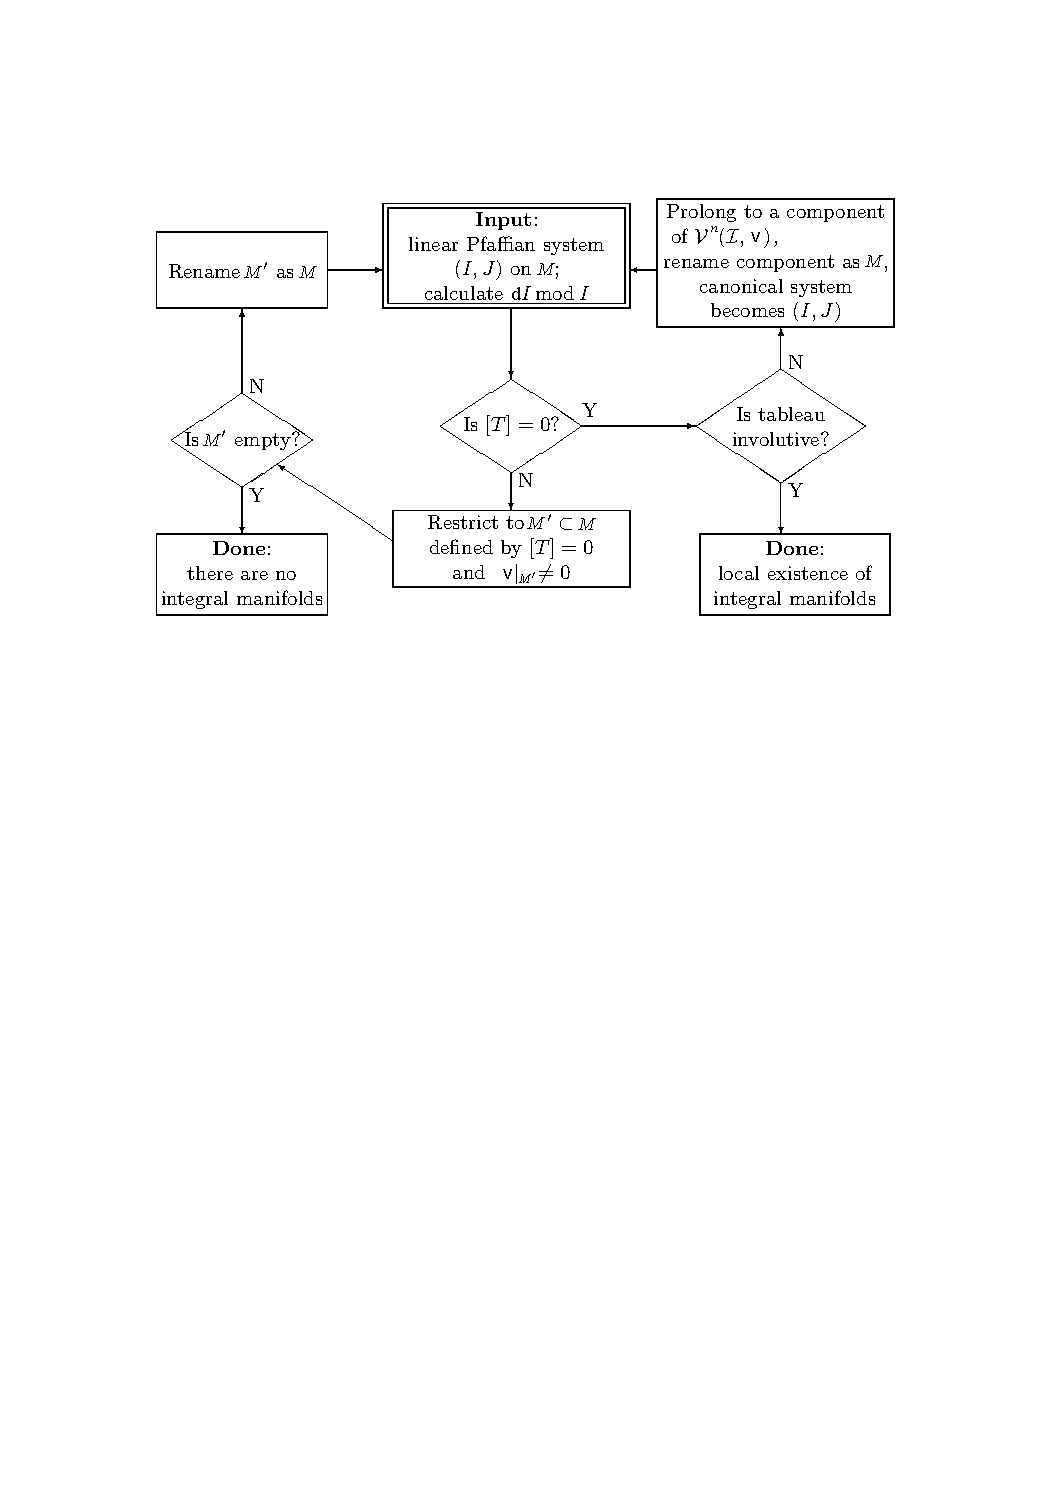
\includegraphics[scale=0.7]{figures/algorithm.pdf}
    \caption{Flow chart of Cartan's algorithm for linear Pfaffian systems. From \cite{Ivey}.}
    \label{fig cartan algorithm}
\end{figure}


\begin{rem}
    \begin{enumerate}
        \item The Cartan algorithm will not necessarily yield all integral manifolds of the original system, only the integral manifolds arising from well-posed Cauchy problems at general points.
        \item Each time one prolongs, there may be many different connected components of $\calV^n(\calI)$ to which one can restrict. To find all possible integral manifolds, one must carry out the algorithm on each component. The Cartan-Kuranishi Prolongation Theorem says in effect that this process terminates eventually, but gives no hint of how long it may take.
        \item How many prolongations it may take for the algorithm to terminate will generally depend on the component one is working with.
    \end{enumerate}
\end{rem}







\section{(*) Cartan-Poincar\'e Lemma}


This \sect\ will be easier to read having some familiarity with homological algebra. First we prove a very basic lemma from exterior algebra, and later generalize it and explain its significance.


\begin{lem}[Cartan]\label{lem cartan}\index{Lemma!Cartan}
    Let $v_1,\ldots,v_k\in V$ be linearly independent elements of a $\bbK$-vector space $V$ and let $w_1,\ldots,w_k\in V$. Then the equation
    \[v_1\wedge w_1+\cdots v_k\wedge w_k=0\]
    holds iff there exists a unique set of scalars $h_{ij}=h_{ji}$, $1\leq i,j\leq k$, such that $w_i=\sum_j h_{ij}v_j$.
\end{lem}
\begin{proof}
    If $V$ is of dimension $n>k$, then let $v_{k+1},\ldots,v_n\in V$ be such that $\{v_i\}_{i=1}^n$ is a basis. Then every $w_j$ can be uniquely written as 
    \[w_i=\sum_{i=1}^n h_{ij}v_j\]
    with some scalars $h_{ij}$, $1\leq i\leq k$, $1\leq j\leq n$. Then, by assumption,
    \[\sum_{i=1}^k\sum_{j=1}^n h_{ij}v_i\wedge v_j=0\]
    By virtue of the antisymmetry of the wedge product, this is equivalent to
    \[\sum_{1\leq i<j\leq k}(h_{ij}-h_{ji})v_i\wedge v_j+\sum_{j=k+1}^n\sum_{i=1}^k h_{ij}v_i\wedge v_j=0.\]
    Since all terms here are linearly independent, this is equivalent to $h_{ij}=0$ for $j>k$, and $h_{ij}=h_{ji}$ for $1\leq i,j\leq k$.
\end{proof}


Let $V,W$ be vector spaces and consider a linear map $\Omega:V\to W$ with dual $\Omega^\ast:W^\ast\to V^\ast$. We set 
\[C^{p,q}\coloneqq \bigodot\nolimits^p W^\ast\otimes \bigwedge\nolimits^q V^\ast.\]
In short, $C^{p,q}$ consists of polynomial exterior forms having polynomial degree $p$ and exterior degree $q$. We now define the \emph{boundary operator}
\begin{gather}
    \delta_\Omega:C^{p,q}\to C^{p-1,q+1},\\
    \delta_\Omega(w_1^\ast\otimes\cdots\otimes w_p^\ast\otimes \psi)=\sum_{i=1}^p w_1^\ast\otimes\cdots\otimes \wh{w}_i^\ast\otimes\cdots\otimes w_p^\ast \otimes \Omega^\ast(w_i^\ast)\wedge\psi,
\end{gather}
where $w_i^\ast\in W^\ast$ and $\psi\in \bigwedge\nolimits^q V^\ast$. As we will see below, this operator is nothing but a the usual exterior derivative which differentiates the $W$-valued coefficients via the map $\Omega$. It is clear that $\delta_\Omega^2=0$, which allows us to define the resulting \emph{cohomology spaces} (quantifying the non-exactness of the sequence) by 
\[\rmH^{p,q}=\bigslant{\ker\left(C^{p,q}\overset{\delta_\Omega}{\to}C^{p-1,q+1}\right)}{\im \left(C^{p+1,q-1}\overset{\delta_\Omega}{\to}C^{p,q}\right)}.\]
The following important result is, as we will see, a generalization of both the Poincar\'e Lemma~\ref{lem poincare classic} and of the Cartan Lemma~\ref{lem cartan}.

\begin{prop}[Cartan-Poincar\'e Lemma {{\cite[Prop.~VIII.2.1]{Bryant}}}]\index{Lemma!Cartan-Poincar\'e}
    There are isomorphisms
    \[\rmH^{p,q}(\Omega)\cong \bigodot\nolimits^p(\ker \Omega^\ast)\otimes \bigwedge\nolimits^q(\coker\Omega^\ast).\]
\end{prop}
\begin{proof}
    \emph{Step One.} First suppose that $\Omega$ is an isomorphism and use it to identify $V$ with $W$. If we choose linear coordinates $x^1,\ldots,x^n$ on $V$, the elements in $C^{p,q}$ are 
    \[\varphi=\sum_{i_1<\cdots<i_q}\varphi_{i_1\ldots i_q}\dd x^{i_1}\wedge\cdots\wedge\dd x^{i_q},\]
    where $\varphi_{i_1\ldots i_q}(\bf{x})\in \bigodot\nolimits^p W^\ast$ is a polynomial of degree $p$. For polynomials, we will simply write $x^i$ instead of $\dd x^i$ because then the commutative product is automatically implied. Thinking of $\Omega$ as the identity map, we have 
    \[\delta_\Omega(x^{j_1}\cdots x^{j_p}\dd x^{i_1}\wedge\cdots\wedge\dd x^{i_q})=\sum_\alpha x^{j_1}\cdots \wh{x}^{j_\alpha}\cdots x^{j_p}\dd x^{j_\alpha}\wedge \dd x^{i_1}\wedge\cdots \wedge\dd x^{i_q}.\]
    This implies that
    \[\delta_\Omega(\varphi)=\dd\varphi\]
    is the usual exterior derivative. We must show that 
    \[\rmH^{p,q}(\Omega)=\begin{cases}
        0, & p+q>0,\\
        \bbR, & p=q=0.
    \end{cases}\label{eq viii.13 Bryant}\]
    Let 
    \[e\coloneqq \sum_i x^i \partial_{x^i}\]
    be the Euler vector field (its flows are homotheties $\bf{x}\mapsto t\bf{x}$).\index{Euler vector field}\index{Homothety} For $\varphi\in C^{p,q}$, Euler's theorem on homogeneous forms implies that 
    \[\Lie_e \varphi=(p+q)\varphi,\]
    where $\Lie_e$ is the Lie derivative along $e$. Combining this with Cartan's magic formula gives the \emph{homotopy formula}
    \[(p+q)\varphi=i_e\dd\varphi+\dd i_e \varphi,\]
    and this implies \eqref{eq viii.13 Bryant}.

    \emph{Step Two.} In the general case, we may choose bases for $V,W$ so that $\Omega$ is a matrix whose top left block is an identity matrix and the rest is zero. Thus, in suitable linear coordinates $(x^i,y^\alpha)$ on $W$ and $(u^\alpha,w^\lambda)$ on $V$ we have 
    \[\Omega^\ast(\dd x^i)=0,\quad \Omega^\ast(\dd y^\alpha)=\dd u^\alpha.\]
    Using multi-index notations, we may write a typical element in $C^{p,q}$ as 
    \[\wt\varphi=\sum_{I,A}\varphi_{IA}(\bf{x},\bf{y})\dd \bf{u}^I\wedge\dd \bf{w}^A,\]
    where $\varphi_{IA}(\bf{x},\bf{y})$ is a polynomial such that $\deg\varphi_{IA}=p$ and $\ord I+\ord A=q$. We shall identify $\wt\varphi$ with the expression 
    \[\varphi=\sum_{I,A}\varphi_{IA}(\bf{x},\bf{y})\dd \bf{y}^I\wedge\dd \bf{w}^A.\]
    When this is done, 
    \[\delta_\Omega(\varphi)=\sum_{I,A}\partial_{y^\alpha}\varphi_{IA}(\bf{x},\bf{y})\dd y^\alpha\wedge\dd \bf{y}^I\wedge\dd \bf{w}^A.\]
    In other words, $\delta_\Omega$ is the exterior derivative w.r.t.\ the $\bf{y}$ variables, treating $\bf{x}$ and $\bf{w}$ as parameters. This suggests that we set 
    \[C^{r,s,\rho,\sigma}\coloneqq \{\varphi\mid \deg_{\bf{x}}\varphi_{IA}=r,\deg_{\bf{y}}\varphi_{IA}=s,\ord I=\rho,\ord A=\sigma\}.\]
    Then $\delta_\Omega:C^{r,s,\rho,\sigma}\to C^{r,s-1,\rho+1,\sigma}$ and with the obvious notation, 
    \[\rmH^{p,q}(\Omega)\cong \bigoplus_{
        \begin{smallmatrix}
            r+s=p\\
            \rho+\sigma=q
        \end{smallmatrix}}\rmH^{r,s,\rho,\sigma}(\Omega).\]
        On the other hand, the proof of Step One gives 
        \[\rmH^{r,s,\rho,\sigma}(\Omega)=\begin{cases}
            0, & \text{unless }s=\rho=0,\\
            C^{r,s,\rho,\sigma}, & \text{when }s=\rho=0.
        \end{cases}\]
        Combining the last two formulas gives the result.
\end{proof}

We will use the Cartan-Poincar\'e Lemma in the following form, which makes it a clear extension of Poincar\'e's Lemma.

\begin{cor}[Cartan-Poincar\'e Lemma {{\cite[Cor.~VIII.2.2]{Bryant}}}]
    Suppose that $\omega^1,\ldots,\omega^n\in V^\ast$ are linearly independent $1$-forms on a vector space $V$ and that $\varphi_{i_1\ldots i_q}\in \bigwedge\nolimits^r V^\ast$ are $r$-forms ($r>0$) that satisfy the conditions 
    \[\left\{
        \begin{array}{l}
            \varphi_{i_1\ldots i_q} \text{ is symmetric in }i_1,\ldots,i_q,\\
            \sum_i \varphi_{i_1\ldots i_{q-1} i}\wedge \omega^i=0.
        \end{array}
    \right.\]
    Then there exist $\psi_{j_1\ldots j_{q+1}}\in \bigwedge\nolimits^{r-1}V^\ast$ that satisfy 
    \[\left\{
        \begin{array}{l}
            \psi_{j_1\ldots j_{q+1}} \text{ is symmetric in }j_1,\ldots,j_{q+1},\\
            \sum_i \varphi_{j_1\ldots j_q j}\wedge \omega^j=\varphi_{j_1\ldots j_q}.
        \end{array}
    \right.\]
\end{cor}
\begin{proof}
    In this case $W=\bbR^n$ and $\Omega:V\to W$ is given by $\Omega(v)=(\omega^1(v),\ldots,\omega^n(v))$, which is surjective. In particular, by the Cartan-Poincar\'e Lemma,
    \[\rmH^{q,r}(\Omega)=0,\quad r>0.\label{eq viii.21 Bryant}\]
    The assumptions of the corollary are 
    \[\delta_\Omega(\varphi)=0,\quad \varphi\in \bigodot\nolimits^q W^\ast\otimes \bigwedge\nolimits^r V^\ast,\]
    and the assertion is that 
    \[\delta_\Omega (\psi)=\varphi,\quad \psi\in \bigodot\nolimits^{q+1}W^\ast\otimes \bigwedge\nolimits^{r-1}V^\ast.\]
    Thus, the corollary is equivalent to \eqref{eq viii.21 Bryant}.
\end{proof}

When $r=q=1$, this corollary is the usual \emph{Cartan Lemma}~\ref{lem cartan}. When $\Omega$ is an isomorphism, it is the Poincar\'e Lemma for polynomial forms.

We now discuss a variant of the lemma relevant to prolongation theory. Let us redefine the spaces $C^{p,q}$ as 
\[C^{p,q}\coloneqq W\otimes \bigodot\nolimits^k V^\ast\otimes \bigwedge\nolimits^q V^\ast.\]
Choosing bases $\{w_a\}$ for $W$ and $\{x^i=\dd x^i\}$ for $V^\ast$ we may think of $\varphi\in C^{k,q}$ as a $W$-valued polynomial form 
\[\varphi=\sum_{\ord I=k,\ord J=q}w_a\otimes \varphi^a_{IJ}\bf{x}^I \dd \bf{x}^J.\]
We define $\delta:C^{k,q}\to C^{k-1,q+1}$ to be the usual exterior derivative treating the $w_a$ as constants. Denoting the resulting cohomology by $\rmH^{k,q}$, we have from Cartan-Poincar\'e Lemma, namely \eqref{eq viii.13 Bryant}, 
\[\rmH^{k,q}=\begin{cases}
    W,& k=q=0,\\
    0, & \text{otherwise}.
\end{cases}\]

Now let $A<W\otimes V^\ast$ be a tableau with prolongations $A^{(q)}<W\otimes \bigodot\nolimits^{p+1}V^\ast$, and define $C^{k,q}(A)<C^{k,q}$ by 
\[C^{k,q}(A)\coloneqq \begin{cases}
    A^{(k-1)}\otimes\bigwedge\nolimits^q V^\ast,& k\geq 1,\\
    W\otimes\bigwedge\nolimits^q V^\ast,& k=0.
\end{cases}\]
The defining property of prolongations, which is that the \emph{total prolongation} $\bf{A}=\bigoplus_{k\geq 0} A^{(k)}$ is the largest graded subspace of the maximal ideal $W\otimes \bigodot\nolimits^{>0}V^\ast$ that is closed under differentiation and satisfies 
\[\bf{A}\cap \left(W\otimes \bigodot\nolimits^{p+1}V^\ast\right)=A,\quad \bf{A}\cap \left(W\otimes\bigodot\nolimits^q V^\ast\right)=0,\quad q\leq p,\]
implies that $\delta$ maps
\[\delta:C^{k,q}(A)\to C^{k-1,q+1}(A),\]
and we denote by $\rmH^{k,q}(A)$ the resulting \emph{Spencer cohomology}:
\[\rmH^{k,q}(A)\coloneqq \bigslant{\ker\left(C^{k,q}(A)\overset{\delta}{\to}C^{k-1,q+1}(A)\right)}{\im \left(C^{k+1,q-1}(A)\overset{\delta}{\to}C^{k,q}(A)\right)}.\]

\begin{rem}\index{Spencer cohomology}
    More explicitly, the Spencer cohomology groups $\rmH^{i,j}(A)$ of a tableau $A<W\otimes V^\ast$ are defined as follows. Let 
    \[\delta_j:(W\otimes \bigodot\nolimits^iV^\ast)\otimes \bigwedge\nolimits^j V^\ast\to W\otimes \bigodot\nolimits^{i-1}V^\ast\otimes \bigwedge\nolimits^{j+1}V^\ast\]
    be defined by 
    \[\delta_j(f\otimes \alpha)=\dd f\wedge \alpha,\]
    where, for $f\in W\otimes \bigodot\nolimits^i V^\ast$, $\alpha\in \bigwedge\nolimits^j V^\ast$, we define $\dd f$ by considering $f$ as an element of $\Hom(V^{\otimes i},W)$, and extend $\delta_j$ by linearity. In simpler terms, $\delta_j$ takes the last index of $f$ and antisymmetrizes over the union of that index with the indices of $\alpha$. Note that $\delta_j(A^{(i)}\otimes \bigwedge\nolimits^j V^\ast)\subset A^{(i-1)}\otimes\bigwedge\nolimits^{j+1}V^\ast$.

    Then 
    \[\rmH^{i,j}(A)= \frac{\ker\restr{\delta_j}{A^{(i-1)}\otimes \bigwedge\nolimits^jV^\ast}}{\im \restr{\delta_{j-1}}{A^{(i)}\otimes \bigwedge\nolimits^{j-1}V^\ast}}.\]
\end{rem}

The main theorem about Spencer cohomology and prolongation, whose proof we omit, is the following.

\begin{thm}[{{\cite[Thm.~VIII.2.4]{Bryant}}}]
    A tableau $A$ is involutive iff $\rmH^{k,q}(A)=0$ for $k\geq 1$, $q\geq 0$.
\end{thm}

From here, it is easy to see that the prolongations of an involutive tableau are involutive. Let $\wt W=A\oplus W$. Then $A^{(1)}$ can be considered as a tableau in $\wt W\otimes V^\ast$ with the $W\otimes V^\ast$ block zero. Consider:
\begin{align}
    \rmH^{0,2}(A^{(1)})&= \frac{\wt W\otimes \bigwedge\nolimits^2 V^\ast}{\delta\left(A^{(1)}\otimes V^\ast\right)}\\
    &= \frac{W\otimes V^\ast\otimes \bigwedge\nolimits^2 V^\ast}{\delta\left(\left((A\otimes V^\ast)\cap (W\otimes \bigodot\nolimits^2 V^\ast)\right)\otimes V^\ast\right)}\\
    &=\rmH^{1,2}(A).
\end{align}
Since prolongations can be defined iteratively, this easily implies that 
\[\rmH^{0,2}(A^{(p)})\cong \rmH^{p,2}(A).\]
In fact, the same argument gives more generally that 
\[\rmH^{k,q}(A^{(p)})\cong \rmH^{k+p,q}(A),\quad k\geq 1.\]
The above theorem then implies that prolongations preserve involutivity. This can be immediately used to show that the prolongation of an involutive linear Pfaffian system is involutive. This is based on the facts, established in \S\ref{sec: lin Pfaffian systems}, that the intrinsic torsion of a linear Pfaffian system  $(\calI,\sfv)$ naturally takes values in $\rmH^{0,2}(A_m)$ and the intrinsic torsion of $(\calI^{(1)},\sfv)$ takes values in $\rmH^{0,2}(A_m^{(1)})\cong \rmH^{1,2}(A_m)$, and if the former vanishes, then so does the latter.

\begin{rem}
    The \emph{Cartan-Kuranishi Prolongation Theorem (1957)}, originally conjectured by Cartan based on numerous examples, implies that after a finite number of prolongations a tableau will become involutive (perhaps by becoming empty, in which case there are no integral manifolds). This implies that, for a linear Pfaffian system on an analytic manifold $M$, if $\rmH^{p,2}(A_m)=0$ for all $p$, then there exist integral manifolds through $m$. This statement is the \emph{Goldschmidt version of Cartan-K\"ahler Theorem}. It is useful because sometimes one can show the vanishing of all groups $\rmH^{p,2}$ without having to compute the prolongations.
\end{rem}







\section{Characteristic variety}



In the Cartan-K\"ahler Theorem~\ref{thm 8.3.3 Ivey} we do not necessarily obtain all solutions to an involutive system by a choice of analytic functions as specified in the theorem. We only obtain those that can be obtained by specifying \emph{noncharacteristic} initial data, that is, initial data based on a choice of a \emph{generic} flag. If we choose a nongeneric flag, the corresponding Cauchy problem may not have any solutions or be undetermined, with an infinite number of solutions. In this \sect\ we formalize this connection between generic flags and characteristic varieties.

Let $M$ be a manifold and denote its tautological $n$-plane bundle by $U\coloneqq \gamma_n(\T M)\to \Gr_n(\T M)$ (cf.\ Definition~\ref{def tautological bundles}). We shall consider the projectivization $\bbP U^\ast$ of the dual bundle $U^\ast$. A point in the fiber $\bbP U^\ast_E$ over some $n$-plane $E\in \Gr_n(\T_m M)$ will be written as $[\xi]$, where $\xi\in E^\ast\setminus\{0\}$ is a nonzero covector and $[\xi]=\<\xi\><E^\ast$ is the corresponding line. By projective duality, $[\xi]$ determines a hyperplane $[\xi]^\perp\coloneqq \Ann(\xi)<E$, and geometrically we may think of $\bbP U^\ast_E$ as being the set of hyperplanes in $E<\T_m M$.

Let $\calI$ be an \gls{eds} on $M$ and assume it has no Cauchy characteristics. This assumption is made merely for convenience and will be eliminated below. Associated to each hyperplane $[\xi]^\perp<E$ is the polar space 
\[H(\xi)\coloneqq H([\xi]^\ast)=\{X\in\T_m M\mid \<\{X\}\cup [\xi]^\perp\>\in\calV(\calI)\},\]
which describes all the ways of extending $[\xi]^\perp$ to an integral $n$-plane.

\begin{defn}[Characteristic variety]\index{Characteristic variety}\label{def char variety eds}
    The (real) characteristic variety of an \gls{eds} $(M,\calI)$ is the subset $\varXi\subset \bbP U^\ast$ defined fiberwise by 
    \[\varXi_E=\{[\xi]\in \bbP E^\ast:E\subsetneqq H(\xi)\},\quad E\in\Gr_n(\T M).\label{eq char variety}\]
    Note that this is non-empty only over integral elements $E$. Thus, $\varXi$ consists of all hyperplanes in integral $n$-planes whose extension to an integral $n$-plane fails to be unique. An integral $(n-1)$-plane $E^{n-1}\in\calV^n(\calI)$ is called \emph{non-characteristic} if $\dim H(E^{n-1})=n$, i.e., if its extension to an integral $n$-plane is unique.
\end{defn}

To the extent that we think of integral elements as infinitesimal solutions to an \gls{eds}, the characteristic variety corresponds to non-uniqueness of an initial value problem, in close analogy to the classical notion. However, unlike in the classical context of differential operators, this definition doesn't require linearization. There is a commuting square 
\[\begin{tikzcd}
    \varXi\arrow[r,hookrightarrow]\arrow[d] & \bbP U^\ast\arrow[d] \\
    \calV^n(\calI)\arrow[r,hookrightarrow] & \Gr_n(\T M).
\end{tikzcd}\]
It is easy to see that the fiber $\varXi_E$ is an algebraic subvariety of $\bbP E^\ast$, i.e., it is defined by polynomial equations. This is because the polar equations are linear in $X\in \T_m M$, and $\varXi_E$ consists of hyperplanes $[\xi]^\perp$ for which the ranks of these equations jump suitably; this condition is expressed by homogeneous polynomial equations in $\xi$. This allows us to also define the \emph{complex characteristic variety} $\varXi^\bbC$ as the set of complex solutions to the same equations. Equivalently, one only needs to replace $E$ in \eqref{eq char variety} with a complex integral element and $[\xi]^\perp$ with a complex hyperplane in $E$, and $\calV(\calI)$ in the definition of $H(\xi)$ with the space of complex integral elements. Of course, it may happen that $\varXi$ is empty but $\varXi^\bbC$ is not.

The reason we assumed no Cauchy characteristics is that $X\in H(\xi)$ for any Cauchy characteristic vector $X$. Thus, the characteristic variety should only be defined for integral elements that contain all Cauchy characteristic vectors. Equivalently, we may consider the \gls{eds} that is the quotient by the Cauchy characteristics and define the characteristic variety of this reduced system. For linear Pfaffian systems this annoyance will be circumvented.

\begin{example}
    \begin{enumerate}
        \item A \emph{Frobenius system} when $\calI$ is generated by $\dd u^1,\ldots,\dd u^s$ in $\bbR^{n+s}$ with coordinates $(x^1,\ldots,x^n,u^1,\ldots,u^s)$. Then $\varXi^\bbC=\varnothing$. A converse of this for involutive systems will be discussed below.
        \item A \emph{Darboux system} when $\calI$ is generated by $\varTheta=\sum_i\dd x^i\wedge\dd y^i$ in $\bbR^{2n}$ with coordinates $(x^1,\ldots,x^n,y^1,\ldots,y^n)$. In this case $\varXi_E=\bbP E^\ast$ is everything.
    \end{enumerate}
\end{example}
\begin{rem}
    Given a differential ideal on a $(2n+1)$-dimensional manifold generated by a single $1$-form $\theta$ satisfying $\theta\wedge(\dd\theta)^{\wedge n}\neq 0$, the Pfaff-Darboux local normal form shows that the maximal integral manifolds $N$, called \emph{Legendre manifolds}, are of dimension $n$ and are given by one arbitrary function of $n$ variables. Here we may think of $\theta=\dd u-\sum_i y_i\dd x^i$ and $N$ given by $(\bf{x},\partial_{\bf{x}}u(\bf{x}))$, where $u(\bf{x})$ is an arbitrary function.
\end{rem}


The most important case is that of linear Pfaffian systems, so we will now show how to define the characteristic variety of such systems in terms of the tableau and the symbol. Recall that a linear Pfaffian system is given by a pair of subbundles $I<J<\T^\ast M$ such that 
\[\dd I\subset \<J\>_{\mathrm{alg}}.\]
(Here we are abusing notation by using the same symbol for a bundle and the space of its sections.) We set $L\coloneqq J\slash I$ so that the exterior derivative induces a bundle map 
\[\wb{\delta}:I\to (\T^\ast M\slash J)\otimes L\]
given in the usual coframe $(\theta^a,\omega^i,\pi^\lambda)$ by the tableau:
\[\wb{\delta}(\theta^a)=A^a_{\lambda i}\pi^\lambda\otimes \omega^i,\]
where the $\omega^i$ are viewed as sections of $L$ and the $\pi^\lambda$ are viewed as sections of $\T^\ast M\slash J$.

Dualizing and using that $(\T^\ast M\slash J)^\ast\cong \Ann(J)<\T M$, giving $\wb\delta$ is equivalent to giving the tableau mapping $\pi$ (cf.~\ref{eq iv.60 Bryant}):
\[\pi:\Ann(J)\to I^\ast\otimes L.\]
The relations on its image, i.e., the tableau bundle $A=\im \pi$, are given by the \emph{symbol map} $\sigma$, which is just the induced quotient map 
\[\sigma:I^\ast\otimes L\to (I^\ast\otimes L)\slash A.\]
Now $\im \pi=\ker\sigma$.

We now define the characteristic variety of a linear Pfaffian system.

\begin{defn}[Characteristic variety of a linear Pfaffian system]
    For each $m\in M$ and $\xi\in L_m\setminus\{0\}$ we let $[\xi]\in \bbP L_m$ be the corresponding line and define the \emph{symbol map at $\xi$} by
    \[\sigma_\xi:I^\ast_m \to (I^\ast \otimes L)_m\slash A_m,\quad w\mapsto \sigma(w\otimes \xi).\]
    The characteristic variety $\varXi\subset\bbP L$ is given fiberwise by 
    \[\varXi_m=\{[\xi]\in \bbP L_m\mid \ker \sigma_\xi\neq \{0\}\}.\]
    In other words, $[\xi]$ is characteristic if there exists a nonzero $w\in I^\ast_m$ such that $w\otimes\xi\in A_m$.
\end{defn}

As we have seen, the symbol map in the usual basis is given by the symbol relations $B^{\lambda i}_a$ defined by the dualized structure equations 
\[B^{\lambda i}_a\pi^a_i\equiv 0\pmod{J}.\]
More precisely, for $\xi=\xi_i\omega^i(m)\in L_m$ as above, $\sigma_\xi$ is given by the matrix
\[\sigma_\xi=\left(B^{\lambda i}_a \xi_i\right)\in \Hom(I^\ast_m,(I^\ast \otimes L)_m\slash A_m).\]
Then 
\begin{align}
    \varXi_m&=\{[\xi]:B^{\lambda i}_a(m)\xi_i w^a=0\text{ for some }w\neq 0\}=\\
    &=\{[\xi]:\rank\left(B^{\lambda i}_a \xi_i\right)<s_0\},
\end{align}
where $s_0=\rank I$. It is clear that $\varXi_m$ is defined by homogeneous polynomial equations in the $\xi_i$, so that each fiber $\varXi_m$ is an algebraic variety.

\begin{rem}
    The way to remember this definition is as follows: associated to a PDE system $F^\lambda(x^i,u^a,u^a_{x^i})=0$ is the canonical contact system $I=\<\theta^a=\dd u^a-p^a_i\dd x^i\>$ on the submanifold in the $(\bf{x},\bf{u},\bf{p})$ space given by $F^\lambda(x^i,u^a,p^a_i)=0$. Differentiating the defining equations of $M$ gives the symbol relations 
    \[F^\lambda_{p^a_i}\dd p^a_i\equiv 0\pmod{J},\quad J=\<\theta^a,\dd x^i\>.\]
\end{rem}

\begin{rem}
    To compare this definition to the more general Definition~\ref{def char variety eds}, recall that Cauchy characteristics are the vector fields $X$ satisfying 
    \[i_X \theta^a=0,\quad i_X\dd\theta^a\equiv 0\pmod{\calI}.\]
    If the $1$-forms $\theta^a,\omega^,\pi^a_i$ fail to span $\T^\ast_m M$ for some $m$, then by our constant rank assumption this will be true in a neighborhood and we can find a vector field satisfying $i_X\theta^a=i_X\omega^i=i_X\pi^a_i=0$. By the structure equation $\dd\theta^a\equiv\pi^a_i\wedge\omega^i\pmod{I}$, this vector field will be a Cauchy characteristic. Thus, under the assumption of no Cauchy characteristics we have 
    \[\T^\ast_m M=\<\theta^a,\omega^i,\pi^a_i\>.\]
    For any integral element $E$ at $m$, the independence condition implies that the restriction map $L_m\to E^\ast$ is an isomorphism. It is now not difficult to show that \emph{under this isomorphism, $\varXi_m\subset \bbP L_m$ corresponds exactly to $\varXi_E\subset \bbP E^\ast$}. See \cite[p.~183]{Bryant} for a proof.
\end{rem}

\begin{rem}
    There is a very simple relation between the Cauchy characteristics and the characteristic variety of a linear Pfaffian differential systems. Let $\<\cha(\calI)\><\T M$ denote the Cauchy characteristic subbundle. Since $\<\cha(\calI)\><\Ann(I)$ the map 
    \[\<\cha(\calI)\>\to L^\ast,\quad X\to \left(\omega^1(X),\ldots,\omega^n(X)\right)\]
    is well-defined, and we denote its image by $S<L^\ast$. Then $\Ann(S)<L$ and we shall show that 
    \[\varXi \subset\bbP \Ann(S).\label{eq v.19 Bryant}\]
    In particular, if $S\neq 0$ then it follows that the fibers $\varXi_m$ of the characteristic variety lie in the proper linear subspaces $\bbP \Ann(S_m)\subset \bbP L_m$. Clearly, \eqref{eq v.19 Bryant} also remains valid when we complexify. In the involutive case, there is a converse to the complex version of \eqref{eq v.19 Bryant}, so $\varXi^\bbC=\bbP\Ann(S^\bbC)$ for involutive systems.

    To prove \eqref{eq v.19 Bryant}, choose a basis $\omega^1,\ldots,\omega^n$ for $L$ so that $\omega^1,\ldots,\omega^k$ is a basis for $\Ann(S)$. Then for $\rho=k+1,\ldots,n$ there is a Cauchy characteristic vector $X_\rho$ satisfying 
    \[i_{X_\rho}\omega^\sigma=\delta^\sigma_\rho,\quad \rho,\sigma=k+1,\ldots,n.\]
    From 
    \[i_{X_\rho}\dd\theta^a\equiv 0\pmod{\calI}\]
    we infer that 
    \[\pi^a_i\equiv 0\pmod{J}.\]
    Thus the tableau matrix looks like 
    \[\begin{pmatrix}
        \pi^1_1 & \cdots & \pi^1_k & 0 & \cdots & 0\\
        \vdots & & & \vdots & & \vdots \\
        \pi^{s_0}_1 & \cdots & \pi^{s_0}_k & 0 & \cdots & 0
    \end{pmatrix}\pmod{J}.\label{eq v.20 Bryant}\]
    In particular, among the symbol relations we have 
    \[\pi^a_\rho \equiv 0\pmod{J},\quad \rho=k+1,\ldots,n.\]
    From this it is easy to see that a characteristic vector $\xi=\xi_i\omega^i$ must have $\xi_{k+1}=\cdots=\xi_k=0$. This proves \eqref{eq v.19 Bryant}.

    We remark that whenever we may choose bases so that the tableau matrix has the block form \eqref{eq v.20 Bryant}, then the zeros correspond to the image $S< L^\ast$ of Cauchy characteristics as described above. We also note that the map $\<\cha(\calI)\>\to S$ may not be injective; using the structure equations $\dd\theta^a\equiv \pi^a_i\wedge\omega^i\pmod{I}$ it is easy to see that this is the case exactly when $\theta^a,\omega^i,\pi^a_i$ fail to span $\T^\ast M$. Examples of this arise by adding extra dummy variables to any Pfaffian system.
\end{rem}


\begin{example}[\ref{ex 5.6.1 Ivey} continued]
    The tableau of \eqref{eq 5.20 Ivey} consists of matrices of the form $\left(\begin{smallmatrix}
        a&b\\b&a
    \end{smallmatrix}\right)$. This has characters $s'_1=2=\dim A$ and $s'_2=0$. A line in $V$ spanned by $\left(\begin{smallmatrix}
        x\\ y
    \end{smallmatrix}\right)$ is characteristic iff the system $ax+by=0$, $bx+ay=0$ on $a,b$ has rank below $2$. Of course, this happens only for the two lines $y=\pm x$. Thus $\varXi_A=\{[1:1],[1:-1]\}$. 
\end{example}

\begin{defn}[Elliptic system]\index{Elliptic!linear Pfaffian system}
    A linear Pfaffian system is called elliptic if its real characteristic variety is empty, $\varXi=\varnothing$.
\end{defn}

\begin{example}[Cauchy-Riemann equations]\label{example cauchy-riemann char variety}
    In $\bbR^{2n}=\bbC^n$ consider the Cauchy-Riemann system 
    \[u_{x^i}-v_{y^i}=0,\quad u_{y^i}+v_{x^i}=0,\quad i=1,\ldots,n.\]
    As we have seen, the symbol matrix of the Pfaffian system corresponding to this PDE is given by its symbol matrix as a PDE:
    \[\begin{pmatrix}
        \xi_1 & \xi_2 & \xi_3 & \xi_4 & \cdots & \xi_{2n-1} & \xi_{2n}\\
        -\xi_2 & \xi_1 & -\xi_4 & \xi_3 & \cdots & -\xi_{2n}& \xi_{2n-1} 
    \end{pmatrix}.\]
    The real characteristic variety is, as expected, empty, so this system is elliptic. However, for each $z\in\bbC^n$ the complex characteristic variety $\varXi^\bbC_z$ is given by the vanishing of all $2\times 2$ minors of this matrix. It is easy to the verify that 
    \[\varXi_z^\bbC=\CP_+^{n-1}\cup \CP^{n-1}_-\subset \CP^{2n-1},\]
    where 
    \[\CP^{n-1}_\pm =\{\xi_2=\pm \i \xi_1,\ldots,\xi_{2n}=\pm \i \xi_{2n-1}\}.\]
    For example, when $n=2$, we may picture $\varXi_z^\bbC$ as two purely imaginary conjugate skew lines in $\CP^3$.
\end{example}


\begin{defn}[Determined system]
    A tableau $A<W\otimes V^\ast$ is called determined if $\dim \Ann(A)=\dim W=s$, i.e., the number of equations is the same as the number of unknowns. A linear Pfaffian system is determined if its symbol matrices are square. 
\end{defn}

\begin{prop}[{{\cite[p.~188]{Bryant}}}]
    Suppose the linear Pfaffian system $(I,J)$ is determined. If for some $\xi\in L_m\setminus\{0\}$, $\det\sigma_\xi\neq 0$, i.e., if the complex characteristic variety is not everything, then the system is involutive at $m$.  
\end{prop}
\begin{proof}
    Writing the symbol relations of a determined system as 
    \[B^{bi}_a\pi^a_i\equiv 0\pmod{J},\]
    we may assume that the characteristic direction is along the $n$'th axis, so $\det\left(B^{bn}_a\right)\neq 0$, and then by a change of basis in the space of relations that 
    \[B^{bn}_a=-\delta^b_a.\]
    The symbol relations become 
    \[\pi^a_n\equiv B^{a\rho }_b\pi^b_\rho\pmod{J},\quad \rho,\sigma=1,\ldots,n-1.\]
    It follows that the characters of the tableau matrix are given by 
    \[s'_1=s_0,\;\ldots,\;s'_{n-1}=s_0,\;s'_n=0.\]
    Now write the symbol relations out as 
    \[\pi^a_n\equiv B^{a\rho }_b \pi^b_\rho +B^a_i\omega^i\pmod{I}.\]
    Integral elements are given by linear equations 
    \[\theta^a=0,\quad \pi^a_i-p^a_{ij}\omega^j=0,\]
    where 
    \[p^a_{ij}=p^a_{ji},\quad p^a_{nj}=B^{a\rho}_bp^b_{nj}+B^a_j.\]
    Choose $p^a_{\rho\sigma}=p^a_{\sigma\rho}$ arbitrarily and use the second relation for $j=1,\ldots,n-1$ to determine the $p^a_{n\sigma}=p^a_{\sigma n}$. Then use the same relation for $j=n$ to determine $p^a_{nn}$. It follows that the $s_0n(n-1)/2$  quantities $p^a_{\rho\sigma}$ specify the integral elements uniquely. We find that 
    \[s_0n(n-1)/2=s'_1+2s'_2+\cdots+ns'_n,\]
    so Cartan's Test is satisfied and the system is involutive.
\end{proof}

% \begin{defn}[Symbol mapping, Characteristic variety]\label{def symbol map}
%     Let $A<W\otimes V^\ast$ be a tableau. For $\alpha\in V^\ast$, define the \emph{symbol mapping} at $\alpha$ by 
%     \[\sigma_\alpha:W\to (W\otimes V^\ast)\slash A,\quad w\mapsto w\otimes\alpha + A.\]
%     Define the \emph{characteristic variety} of $A$, $\varXi_A\subset \bbP V^\ast$ (where $\bbP$ stands for the projectivization functor $V\mapsto V\slash \bbK^\times$ for $\bbK$-vector spaces), to be the set of all \emph{characteristic hyperplanes} (codimension $1$ subspaces) in $V$:
%     \[\varXi_A\coloneqq \{[\alpha]\in \bbP V^\ast\mid \ker \sigma_\alpha\neq 0\}.\]
%     We interpret $\varXi_A$ is the set of hyperplanes in $\bbP V$ for which the extension of an $(n-1)$-dimensional integral element to an $n$-dimensional one is not unique, see Theorem~\ref{thm 6.7.7 Ivey}.
% \end{defn}


% Even when we are only interested in real solutions of the underlying PDE, it is useful to consider the \emph{complex characteristic variety}
% \[\varXi^\bbC_A\coloneqq \{[\alpha]\in \bbP (V^\ast)^\bbC\mid \ker \sigma_\alpha^\bbC\neq 0\},\]
% where $\sigma^\bbC_\alpha:W^\bbC\to (W^\bbC\otimes (V^\ast)^\bbC)\slash A^\bbC$ is the complexification of $\sigma_\alpha$ (see Definition~\ref{def complexification}).





\section{Properties of the characteristic variety}

We now discuss some key properties of the characteristic variety. In doing so, we will omit many proofs, referring the reader to \cite[Ch.~V]{Bryant} instead.

\paragraph{(i) The first derived system and $\varXi$.} The first property deals with a natural subsystem that will turn out being irrelevant to the computation of the characteristic variety.

\begin{defn}[Derived system]
    Let $I<\T^\ast M$ be a Pfaffian system of constant rank. The derived system $I_{(1)}$ of $I$ is the subbundle spanned by $I$-valued forms whose exterior derivatives modulo $I$ vanish. More explicitly, let $\delta:\Gamma^\infty(I)\to \Gamma^\infty\left(\bigwedge\nolimits^2(\T^\ast M\slash I)\right)$ be defined by \[\delta(\theta)=\dd\theta\mod I.\] 
    
    Because $\delta$ is $C^\infty(M)$-linear, it is induced by a \gls{vb} morphism $\delta:I\to \bigwedge\nolimits^2(\T^\ast M\slash I)$. Since the coefficients of $\delta$, when expressed in matrix form, are smooth, its rank is upper semicontinuous, so we may restrict to an open set in $M$ on which it has constant rank. On this open set, we define $I_{(1)}\coloneqq \ker\delta$. We have the exact sequence 
    \[0\to I_{(1)}\to I\overset{\delta}{\to}\dd I\slash \<I\>_{\mathrm{alg}}\to 0.\]
    
    If $I_{(1)}=I$, then $I$ is Frobenius; otherwise, $I_{(1)}$ is smaller. In that case, we define a sequence of systems iteratively by $I_{(k+1)}=(I_{(k)})_{(1)}$, until $I_{(N)}$ is either Frobenius ($I_{(N+1)}=I_{(N)}$) or rank zero. The \emph{derived flag} is 
    \[I=I_{(0)}> I_{(1)}>\cdots >I_{(N)},\]
    and $N$ is the \emph{derived length}.
\end{defn}

For an adapted basis $(\theta^1,\ldots,\theta^p;\theta^{p+1},\ldots\theta^{s_0})=(\theta^\rho,\theta^\epsilon)$ for $I_{(1)}<I$ (here $\rho,\sigma=1,\ldots,p$ and $\epsilon,\delta=p+1,\ldots,s_0$) we have 
\[\dd \theta^\rho\equiv 0\pmod{I},\quad \dd\theta^\epsilon\equiv \pi^\epsilon_i\wedge\omega^i\pmod{I}.\]
The symbol relations are of the form 
\[\pi^\rho_i\equiv 0\pmod{J},\quad B^{\lambda i}_\epsilon\pi^\epsilon_i\equiv 0\pmod{J},\]
and the tableau matrix is 
\[\begin{bmatrix}
    0\\\pi^\epsilon_i
\end{bmatrix}.\]
In intrinsic terms, we have the dualized exact sequence 
\[0\to (I\slash I_{(1)})^\ast\to I^\ast\to I^\ast_{(1)}\to 0.\]
The tableau corresponding to the above matrix is given by a subbundle $A<I^\ast\otimes L$ with the property that $A$ projects to zero in $I^\ast_{(1)}\otimes L$, i.e.,
\[A<(I\slash I_{(1)})^\ast \otimes L<I^\ast\otimes L.\]
For $\xi\in L\setminus\{0\}$ the symbol map $\sigma_\xi:I^\ast\to (I^\ast\otimes L)\slash A$ restricts to 
\[\sigma_{(1),\xi}:(I\slash I_{(1)})^\ast\to (I^\ast\otimes L)\slash A,\]
and from the definitions it follows that 
\[\ker\sigma_\xi=\ker\sigma_{(1),\xi}.\]
Thus the characteristic variety is the same as if we consider only the bottom nonzero block in the tableau matrix, i.e., we consider only the ``smaller'' symbol matrices $\left(B^{\lambda i}_\epsilon \xi_i\right)$. Informally, 
\begin{quote}
    \emph{In computing the characteristic variety, we can ignore the derived system.}
\end{quote}
This property is a generalization of the fact that the symbol and the characteristic variety of a PDE depend only on its highest order terms.

\paragraph{(ii) Characteristic variety of the prolongation.}

Recall that the first prolongation $(\calI^{(1)},\sfv)$ is defined on the manifold $M^{(1)}$, which is a connected component of the space of ordinary integral elements of $(\calI,\sfv)$, and as a Pfaffian system $I^{(1)}$ is generated by the equations 
\[\theta^a=0,\quad \theta^a_i=\pi^a_i-p^a_{ij}\omega^j=0,\quad B^{\lambda i}_ap^a_{ij}=0.\label{eq v.76 Bryant}\]
The exterior derivatives of these equations give, using the original structure equations, 
\[\dd\theta^a\equiv 0\pmod{I^{(1)}},\quad\dd\theta^a_i\equiv \pi^a_{ij}\wedge\omega^j\pmod{I^{(1)}},\label{eq v.77 Bryant}\]
where locally $\<I^{(1)}\>=\<\theta^a,\theta^a_i\>$ and 
\[\pi^a_{ij}=-\dd p^a_{ij}+(\text{pullbacks of forms on $M$ to }M^{(1)}).\]
Comparing \eqref{eq v.76 Bryant} and \eqref{eq v.77 Bryant} we see as before that the original Pfaffian system is contained in the first derived system of the prolongation, and hence, by  property (i), when computing the characteristic variety of $\calI^{(1)}$ we need only consider the tableau $\left(\pi^a_{ij}\right)$. Differentiating the last equation in \eqref{eq v.76 Bryant} and using that pullbacks of forms on $M$ are spanned by $\<\theta^a,\omega^i,\pi^a_i\>=\<\theta^a,\omega^i,\theta^a_i\>$, it follows that the symbol relations on the $\pi^a_{ij}$ are 
\[\pi^a_{ij}\equiv \pi^a_{ji}\pmod{\theta^b,\theta^b_i,\omega^i},\quad B^{\lambda i}_a\pi^a_{ij}\equiv 0\pmod{\theta^b,\theta^b_i,\omega^i}.\]
Note that the second set of relations is indexed by $(\lambda,j)$. Thus, we should write these relations as 
\[B^{(\lambda,j)ik}_a \pi^a_{ik}\equiv 0 \pmod{\theta^b,\theta^b_a,\omega^i},\]
where 
\[B^{(\lambda,j)ik}_a=\delta^i_k B^{\lambda i}_a.\]
If $\xi=(\xi_i)$ is characteristic for $(\calI^{(1)},\sfv)$, then there exists a $w=(w^a_i)$ satisfying 
\[w^a_i\xi_j=w^a_j\xi_i,\quad B^{(\lambda,j)ik}_aw^a_i\xi_k=0.\]
From the first relation we have $w^a_i=w^a\xi_i$, and from the second $B^{\lambda i}_aw^a\xi_i\xi_j=0$, $j=1,\ldots,n$. It follows that 
\[B^{\lambda i}_aw^a\xi_i=0,\]
which says that $\xi$ is characteristic for $(\calI,\sfv)$. Since the converse is obviously true, we have established that under the projection $\pi:M^{(1)}\to M$,
\[\text{\emph{There is a natural isomorphism }} \varXi^{(1)}_q\cong \varXi_{\pi(q)}\text{ for all } q\in M^{(1)}.\]
In other words, in the absence of integrability conditions (i.e., if the intrinsic torsion is identically zero), the characteristic variety doesn't change upon prolongation. If there are integrability conditions $[T]=0$, then they will contribute additional symbol relations to the prolonged system, so the characteristic variety may get smaller: $\varXi^{(1)}_q\subset \varXi_{\pi(q)}$.


\paragraph{(iii) Characteristic variety and the Cartan-K\"ahler Theorem.} The remaining properties are more substantial and require involutivity. We discuss them briefly without derivation. Recall that if $\kappa=s_l$ is the top nonzero Cartan character of the system, then it integral manifolds depend on $\kappa$ functions of $l$ variables. To an algebraic geometer, $l$ resembles a transcendence degree and $\kappa$ a field extension degree -- this analogy will turn out to be precise. We will state results that express $l,\kappa$ and the condition to be a regular flag in terms of algebro-geometric properties of the complex characteristic variety $\varXi^\bbC$. In practice these theorems usually allow one to determine $l,\kappa$ and regular flags without going through the sometimes laborious procedure of calculating the $s'_p$. 

If $\varXi^\bbC=\bigcup_\alpha \varXi^{\bbC,\alpha}$ is the unique (fiberwise) decomposition of $\varXi^\bbC$ into irreducible components (i.e., each component is defined by an irreducible system of polynomials), then we define 
\[d^\alpha\coloneqq \dim_\bbC\varXi^\bbC_m,\quad \delta^\alpha(m)\coloneqq \deg \varXi_m^{\bbC,\alpha},\quad \mu^\alpha(m)\coloneqq \dim\ker\sigma_{m,\xi},\]
where $[\xi]\in \varXi^\bbC_m$ is a general point. As a consequence of involutivity, all of these integers are independent of $m\in M$. We further define 
\[d\coloneqq \max_\alpha d^\alpha,\quad \delta(m)\coloneqq \sum{}'\delta^\alpha(m),\quad\mu(m)\coloneqq \sum{}'\mu^\alpha(m),\]
where $\sum{}'$ denotes the sum over components of the maximal dimension, $d$. Again, $d$, $\delta$, and $\sum{}'\mu^\alpha(m)\delta^\alpha(m)$ will be independent of $m$. The main result is the following.

\begin{thm}[{{\cite[Thm.~V.3.6]{Bryant}}}]\label{thm v.3.6. Bryant}
    Let $(\calI,\sfv)$ be an involutive Pfaffian system of character $l$ and Cartan integer $\kappa=s_l$. Then, with the above notation, 
    \[l=d+1,\quad \kappa=\sum{}'\mu^\alpha(m)\delta^\alpha(m).\]
\end{thm}

\begin{cor}[{{\cite[Cor.~V.3.7]{Bryant}},{\cite[Thm.~5.6.12]{Ivey}}}]
    Suppose that all $\mu^\alpha(m)=1$ (this is often the case). Then 
    \[l=\dim_\bbC \varXi^\bbC_m+1,\quad \kappa=\deg \varXi^\bbC_m.\]
\end{cor}

If we omit reference to the point $m$, we may rephrase this as 
\begin{quote}
    \emph{The integral manifolds of an involutive, analytic Pfaffian system locally depend on $\deg\varXi^\bbC$ functions of $\dim_\bbC\varXi^\bbC+1$ variables.}
\end{quote}

\begin{example}[\ref{example cauchy-riemann char variety} continued]
    The characteristic variety of the Cauchy-Riemann system has $\delta^1=\delta^1=\mu^1=\mu^2=1$, so 
    \[d=n-1,\quad \kappa=2,\]
    so we get the familiar result that holomorphic maps of $n$ complex variables depend on $2$ functions of $n$ real variables.
\end{example}

\begin{cor}[{{\cite[Cor.~V.3.11]{Bryant}}}]\label{cor v.3.11 Bryant}
    Let $(\calI,\sfv)$ be a smooth involutive linear Pfaffian system whose complex characteristic variety is empty, $\varXi^\bbC=\varnothing$. Then $\calI$ is completely integrable: through each point of $m$ there passes a unique integral manifold of $\calI$.
\end{cor}
\begin{proof}
    By Theorem~\ref{thm v.3.6. Bryant}, $l=1$ and $\kappa=0$, so we have $s_1=\cdots=s_n=0$, and since there are no integrability conditions, the structure equations are $\dd\theta^a\equiv 0\pmod{\theta^b}$. Thus, the Frobenius condition $\dd I\equiv 0\pmod{I}$ is satisfied.
\end{proof}

A final theorem following from this result is the following.

\begin{thm}[{{\cite[Thm.~V.3.12]{Bryant}}}]
    Let $(\calI,\sfv)$ be an \gls{eds} and assume that:
    \begin{enumerate}[label=(\roman*)]
        \item $\varXi^\bbC=\varnothing$;
        \item the process of prolongation is well-behaved: at each stage we get a locally finite union of manifolds (this is automatic for real analytic systems).
    \end{enumerate}
    Then some prolongation of $(\calI,\sfv)$ is either empty or is a Frobenius system. In particular, for a suitable $q$ each connected integral manifold of $(\calI,\sfv)$ is uniquely determined by its $q$-jet at one point.
\end{thm}
\begin{proof}
    Based on Theorem~\ref{thm vi.2.1 Bryant}, a suitable prolongation $(\calI^{(q)},\sfv)$ is either empty or involutive. Since integral manifolds of $(\calI^{(q)},\sfv)$ are in local one-to-one correspondence with those of $(\calI,\sfv)$, we may focus on the involutive case.  Since prolongation preserves the characteristic variety, $\varXi^{\bbC,(q)}$ is empty. By Corollary~\ref{cor v.3.11 Bryant}, $(\calI^{(q)},\sfv)$ is Frobenius and its integral manifolds are uniquely specified by a choice of a single point of $M^{(q)}$, i.e., by the $q$-jet of the corresponding integral manifold of $(\calI,\sfv)$.
\end{proof}

Informally, we may say that \emph{in the case $\varXi^\bbC=\varnothing$ the integral manifolds depend on a finite number of constants}, which is a generalization of the concept of complete integrability.

\paragraph{(iv) Characteristic variety and K\"ahler-singular elements.} We have defined the characteristic variety in terms of the characteristic, or singular, hyperplanes in $n$-dimensional integral elements. On the other hand, if $(\calI,\sfv)$ is an involutive Pfaffian system of character $l$, then the uniqueness of extensions in the Cauchy problem for $n$-dimensional integral manifolds occurs along $l$-dimensional submanifolds. Thus, we may expect that the characteristic variety should consist of singular $l$-dimensional integral elements. In other words, when $l<n-1$ (roughly speaking, this is the \emph{overdetermined case}), there are two possible characteristic varieties, and it is obviously important to relate them.

Recall that an integral element $E\in\calV^n(\calI)$ is K\"ahler-regular if the rank of the polar equations is locally constant near that element in $\calV^n(\calI)$. Otherwise we call it \emph{K\"ahler-singular}. In terms of the characters, singularity is equivalent to being \emph{non-generic}: a $p$-plane $E^p$ is singular if the total number $s(E^p)$ of polars in a tableau adapted to $E^p$ (this number depends only on $E^p$ itself) is strictly less than the character sum (which characterizes the generic integral $p$-plane). We define 
\[\varLambda_p\coloneqq \{E\in \calV^p(\calI)\subset \Gr_p(L^\ast)\mid s(E)<s'_1+\cdots+s'_p\}.\]
If the character of the system is $l$, then $\varLambda\coloneqq \varLambda_l$ is called the \emph{Cartan characteristic variety}. 

If there are no integrability conditions, i.e., the symbol relations may be assumed to be 
\[B^{\lambda i}_a \pi^a_i\equiv 0\pmod{I},\]
then $\varLambda_p$ us the set of integral $p$-planes whose polar equations have lower rank than the generic integral $p$-plane. In particular, in the absence of integrability conditions, $\varLambda_{n-1}=\varXi$.

According to the Cartan-K\"ahler Theorem, the Cartan characteristic variety determines the set of integral elements that are characteristic for the last Cauchy-Kovalevskaya system in which there is any freedom in assigning initial data. It is clear how to define $\varLambda_p^\bbC$ and $\varLambda^\bbC$. The main result relating the Cartan characteristic variety to the usual characteristic variety is the following.

\begin{thm}[{{\cite[Thm.~V.3.15]{Bryant}}}]\label{thm v.3.15 Bryant}
    If $(\calI,\sfv)$ is involutive and of character $l$, then 
    \begin{align}
        \varLambda^\bbC&=\{E\in \Gr_l(L^{\ast,\bbC})\mid E\in [\xi]^\perp \text{ for some characteristic }[\xi]\in\varXi^\bbC\},\\
        \varXi^\bbC&=\{[\xi]\in\bbP L^\bbC\mid E\in \varLambda^\bbC \text{ for all subspaces }E<[\xi]^\perp\}.
    \end{align}
\end{thm}

Note that since we may have $\varXi=\varnothing$ but $\varLambda\neq \varnothing$, the analogous statement is false over $\bbR$. What we can say is that the \emph{real} Cartan characteristic variety $\varLambda$ is given in terms of the \emph{complex} usual characteristic variety by 
\[\varLambda=\{E\in\Gr_l(L^\ast)\mid E<[\xi]^\perp \text{ for some characteristic }[\xi]\in\varXi^\bbC\}.\label{eq v.102 Bryant}\]
Similarly, the second assertion in Theorem~\ref{thm v.3.15 Bryant} gives $\varXi^\bbC$ in terms of $\varLambda^\bbC$ as follows: an $(n-1)$-plane is characteristic iff \emph{every} $l$-plane contained in it is Cartan characteristic.

\begin{example}[\ref{example cauchy-riemann char variety} continued]
    Consider again the Cauchy-Riemann system on $\bbR^{2n}\cong \bbC^n$, now with the standard complex structure $\sfJ:\bbR^{2n}\to \bbR^{2n}$ given by 
    \[\sfJ(\partial_{x^i})=\partial_{y^i},\quad \sfJ(\partial_{y^i})=-\partial_{x^i}.\]
    We've already seen that this system is elliptic, so $\varXi=\varnothing$. To describe the Cartan characteristic variety, since the system is translation invariant it will suffice to describe the fiber $\varLambda_0$ of $\varLambda$ over the origin, and using \eqref{eq v.102 Bryant} this is given by 
    \[\varLambda_0=\{E\in\Gr_n(\bbR^{2n}):E\cap \sfJ(E)\neq \{0\}\}.\]
    In other words, $\varLambda_0$ consists of real $n$-planes that contain at least one \emph{complex line} (i.e., a \emph{real} $\sfJ$-invariant $2$-plane). 

    It is, of course, well known that real $n$-dimensional submanifolds $Y^n\subset \bbC^n$ such that $\T_y Y\cap \sfJ(\T_y Y)=\{0\}$ for every $y\in Y$ are locally determining sets for holomorphic functions. 

    In general we have 
    \[\varLambda_{p,0}=\{E\in\Gr_p(\bbR^{2n})\mid \dim E\cap \sfJ(E)\geq \max(1,2(p-m)+1)\}.\]
    For instance, $\varLambda_{2m-1,0}=\Gr_{2m-1}(\bbR^{2n})$ contains no information.
\end{example}

\paragraph{(v) Integrability of the characteristic variety.} Let us define the concept of involutivity for the characteristic variety.

\begin{defn}[Eikonal equation I]
    Let $N$ be a manifold and $\varSigma\subset \bbP \T^\ast N$ a subset. The associated eikonal equation $E_\varSigma\subset C^\infty(N)$ is defined as follows: a function $\varphi\in C^\infty(N)$ is a solution of $E_\varSigma$ if $[\dd \varphi(x)]\in \varSigma_x$ for all $x\in N$ such that $\dd \varphi(x)\neq 0$.
\end{defn}

For another description, let $\wt\varSigma\subset\T^\ast N$ be defined by 
\[\wt\varSigma=\pi^{-1}(\varSigma)\cup \{0\}\subset \T^\ast N,\]
where $\pi:\T^\ast N\setminus \{0\}\to \bbP \T^\ast N$ is the projectivization map and $\{0\}\subset \T^\ast N$ denotes the zero section. Then $\wt\varSigma$ is a \emph{conical subvariety} of $\T^\ast N$, i.e., it is invariant under scaling of the fibers. Moreover, any conical subvariety is of this form. Then solutions to the eikonal equation are characterized by $\dd\varphi(x)\in \wt\varSigma$. 

If $x^1,\ldots,x^n$ are local coordinates on $N$ with induced coordinates $(x^i,\xi_i)$ on $\T^\ast N$, then we shall always assume that $\varSigma$ is a subset with the property that $\wt\varSigma$ is defined by equations 
\[F^\lambda(y^i,\xi_i)=0,\quad \lambda=1,\ldots,R,\]
where the $F^\lambda$ are either smooth or analytic depending on the category in which we are working.

\begin{defn}[Eikonal equation II]
    The eikonal differential equation is a PDE for functions $\varphi\in C^\infty(N)$ of the form
    \[F^\lambda\left(\bf{y},\partial_{\bf{y}}\varphi(\bf{y})\right)=0,\quad \lambda=1,\ldots,R.\]
\end{defn}

\begin{rem}
    The functions $F^\lambda$ need only be defined \emph{microlocally}, i.e., in open sets $U\subset \T^\ast N$ invariant under scaling. In the cases of interest to us the fibers $\varSigma_x$ of $\varSigma\to N$ will be algebraic varieties, so that the $F^\lambda(x^i,\xi_i)$ may be chosen to be homogeneous polynomials in the $\xi_i$, whose coefficients are functions of the $x^i$. In this case, the complexifications 
    \[\varSigma^\bbC\subset \bbP \T^{\ast,\bbC}N,\quad \wt{\varSigma}^\bbC\subset \T^{\ast,\bbC}N\]
    are naturally defined, and so the complex eikonal equation makes sense by allowing the function $\varphi$ to have complex values and requiring that $\dd\varphi\in\wt{\varSigma}^\bbC$. We remark that we may have $\varSigma=\varnothing$ but $\varSigma^\bbC\neq\varnothing$. \emph{From now on we assume that the $F^\lambda$ may be chosen to be homogeneous polynomials in the $\xi_i$}.
\end{rem}

\begin{defn}[Involutive conical subvariety]
    The subset $\varSigma^\bbC\subset \bbP \T^{\ast,\bbC}N$ is called involutive in case the eikonal equation $E_{\varSigma^\bbC}$ is involutive.
\end{defn}

To state the main result, we let $\calI$ be a different system on a manifold $M$ with complex characteristic variety $\varXi^\bbC\subset \bbP U^{\ast,\bbC}$ (cf.~the definitions at the start of this \sect). For any integral manifold $i:N\to M$ of $\calI$ there is the \emph{induced characteristic variety}
\[\varXi_N^{\bbC}\subset \bbP \T^{\ast,\bbC}N\]
defined as follows. We have the diagram 
\[\begin{tikzcd}
     & \bbP U^{\ast,\bbC} \arrow[dl,dashed]\arrow[d,"\wt\pi"]\\
     \bbP \T^{\ast,\bbC}N\arrow[d] \arrow[r,"\wh{i}_\ast"] & \Gr_n(\T M)\arrow[d]\\ 
     N\arrow[r,hookrightarrow,"i"] & M,
\end{tikzcd}\]
where 
\[\wh{i}_\ast(x)=i_\ast(\T_x N),\quad \wt{\pi}^{-1}(m,E)=\bbP E^{\ast,\bbC}.\]
The condition that $N$ be an integral manifold of $\calI$ is that 
\[\wt{\pi}^{-1}(\wt{i}_\ast(N))\to \bbP \T^{\ast,\bbC}N.\]
By definition, $\varXi^\bbC_N$ is the image of $\varXi^\bbC\cap \wt{\pi}^{-1}(\wt{i}_\ast(N))$ under this mapping. Informally, $\varXi^\bbC_N$ \emph{is induced from the characteristic variety $\varXi^\bbC$ in each of the integral elements $i_\ast(\T_x N)\in \Gr_n(\T M)$}.

\begin{defn}[Involutive characteristic variety]
    The characteristic variety $\varXi^\bbC$ is called \emph{involutive} if the eikonal equation $E_{\varXi^\bbC_N}$ is involutive for any integral manifold $N$ of $\calI$.
\end{defn}

The following fundamental result essentially states that \emph{if $\calI$ is involutive, then its characteristic variety is involutive}. 

\begin{thm}[Cartan, Guillemin, Quillen, Sternberg, Gabber ('53-'81) {{\cite[Thm.~V.3.20]{Bryant}}}]
    Let $E\in \calV_n(\calI)$ be an ordinary integral element. Then $\varXi^\bbC$ is involutive in an open neighborhood $V$ of $E$.
\end{thm}
What this means is that $\varXi^\bbC_N$ is involutive for all integral manifolds $i:N\to M$ satisfying $\wt{i}_\ast(N)\subset V$.

% Let us now \emph{work over $\bbC$ and drop $\bbC$ from the notation}. We estimate the dimension of $\varXi_A$ and a modification of the degree of $\varXi_A$ in terms of the characters of $A$. We use the convention that the empty set has dimension $-1$, and denote the modified degree defined below by $\widetilde{\deg}$.

% Now suppose $(I,J)$ has no intrinsic torsion and let $E\in\calV^n(I,J)_m$. Let $H<E$ be a hyperplane, i.e., $\dim H=n-1$. We address the following question: under what circumstances is $E$ the only integral $n$-plane that contains $H$?

% \begin{defn}[Characteristic hyperplane]
%     A hyperplane $H<E<\T_mM$ is said to be characteristic if it has more than one extension to an $n$-dimensional integral element.
% \end{defn}

% With notation as above, we may choose the coframe so that 
% \[\restr{\theta^a}{E}=\restr{\pi^a_i}{E}=0.\]
% Assume moreover that $E$ is uniquely defined by these equations, that is, $\{\theta^a,\omega^i,\pi^a_i\}$ span $\T_m^\ast M$ (so there are no Cauchy characteristics).

% We can also choose frames so that $\restr{\omega^n}{H}=0$. Let $e_1,\ldots,e_n$ be a basis for $E$ dual to $\{\omega^i\}$. Then $v\in \T_mM\setminus H$ completes $H$ to an integral $n$-plane iff 
% \[\forall\varPhi \in\calI^n\quad \varPhi (v,e_1,\ldots,e_{n-1})=0.\label{eq 6.17 Ivey}\]
% In fact, it is sufficient to require that $i_v \theta^i=0$ and to verify \eqref{eq 6.17 Ivey} for $\varPhi=\pi^a_i\wedge \omega^J$, where $J$ is any multi-index of length $n-1$ containing the index $i$. Since $i_{e_i}\pi^\lambda=0$, \eqref{eq 6.17 Ivey} becomes 
% \[i_v\pi^a_i=0,\quad  \forall a, i=1,\ldots,n-1.\label{eq 6.18 Ivey}\]
% Now recall the symbol mapping from Definition~\ref{def symbol map}, defining the characteristic variety $\varXi_A$ for $A=A_m$. If $\alpha_H\in \bbP E^\ast$ corresponds to $H<E$, then $\alpha_H\in \varXi_A$ iff 
% \[B^{rn}_a w^a=0\]
% for some nonzero $w\in W$. In other words, $\alpha_H\in\varXi_A$ iff the tableau contains a matrix with the first $n-1$ columns zero and the last column nonzero, or equivalently, some linear combination of the $\pi^a_n$ is linearly independent from the forms in the first $n-1$ columns, so that $v$ is not uniquely determined by \eqref{eq 6.18 Ivey}. We have now proved 
% \begin{thm}
%     A hyperplane $H<E<\T_mM$ is characteristic iff the corresponding element $\alpha_H\in\bbP E^\ast$ is in $\varXi_A$.
% \end{thm}








\section{Hyperbolic second-order \texorpdfstring{\glspl{eds}}{EDSs}}\label{sec: hyperbolic EDS}

We wrap up the chapter by considering some special systems, related to second-order PDEs, that we will encounter in the study of surfaces in the next \chap. A general classification of second-order PDEs based on the geometry of their integral manifolds is possible but is quite lengthy, so we direct the reader to \cite[\S VII.1]{Bryant} for that. Instead, we will focus on a specific method developed for \emph{hyperbolic second-order equations}, which are distinguished by the fact that their characteristic variety is given by a quadratic equation with two distinct real roots.

We consider a general second-order PDE for a function of two variables as an \gls{eds}. We use the coordinates $(x,y,z,p,q,r,s,t)$ on $\rmJ^2(\bbR^2,\bbR)$ and contact forms 
\[\theta_0=\dd z-p \dd x-q\dd y,\quad \theta_1=\dd p-r\dd x-s\dd y,\quad \theta_2=\dd q-s\dd x-t\dd y.\]
Suppose the PDE takes the form 
\[F(x,y,z,p,q,r,s,t)=0\label{eq 7.10 Ivey}\]
and that this equation defines a smooth submanifold $M^7<\rmJ^2(\bbR^2,\bbR)$, and that at least one of the partial derivatives $F_r,F_s,F_t$ is nonzero at each point of $M$, and say that $F$ is \emph{regular} when these assumptions hold. Regularity ensures that $\theta_0,\theta_1,\theta_2$ restrict to be linearly independent on $M$, and that the projection $\pi:M\to \rmJ^1(\bbR^2,\bbR)$ is a smooth submersion at each point. 

Let $I$ be the Pfaffian system spanned by the restrictions of $\theta_1,\theta_2,\theta_3$ to $M$. Since $\dd\theta_0\equiv 0\pmod{I}$, the ideal $\calI=\<I\>_{\mathrm{diff}}$ is generated algebraically by $I$ and the $2$-forms 
\[\dd\theta_1=-(\dd r\wedge \dd x+\dd s\wedge \dd y),\quad \dd\theta_2=-(\dd s\wedge\dd x+\dd t\wedge\dd y).\]
We could write down the tableau immediately, but before doing so it is useful to find a coframe in which the symbol relation has the simplest form. Near any point in $M$, one can obtain $1$-forms $\pi_1,\pi_2,\pi_3$ such that 
\begin{align}
    \dd\theta_1& \equiv -(\pi_1\wedge \dd x+\pi_2\wedge\dd y )\pmod{I} \\
    \dd\theta_2& \equiv -(\pi_2\wedge\dd x+\pi_3\wedge\dd y) \pmod{I}
\end{align}
and such that they satisfy the symbol relation 
\[F_r\pi_1+F_s\pi_2+F_t\pi_3\equiv 0\pmod{I}.\label{eq 6.15 Ivey}\]
For example, if $F_r\neq 0$, we may choose 
\begin{align}
    \pi_1&= \dd r+\frac{F_rD_xF-F_sD_yF}{F_r^2}\dd x+\frac{D_y F}{F_r}\dd y,\\
    \pi_2&=\dd s+\frac{D_y F}{F_r}\dd x,\\
    \pi_3&=\dd t.
\end{align}
where $D_xF=F_x+pF_z+rF_p+sF_q$ and $D_yF=F_y+qF_z+sF_p+tF_q$.

Let $u\in M$ and let $E\in \calV^2(\calI)$ be an integral $2$-plane at $u$. If we use the bases $\{\theta_0,\theta_1,\theta_2\}$ for $W^\ast=I_u$ and $\{\dd x,\dd y\}$ for $E^\ast\cong V^\ast=(J\slash I)_u$, then \eqref{eq 6.15 Ivey} shows that the tableau has the form 
\[A_u=
    \left\{
\begin{pmatrix}
    0 & 0\\
    a & b\\
    b& c
\end{pmatrix}
    \middle| aF_r(u)+bF_s(u)+cF_t(u)=0
    \right\}<W\otimes V^\ast.
\]

Applying Cartan's Test to the tableau shows that such systems are involutive with solutions depending locally on $s_1=2$ functions of one variable. Although there is usually no explicit way to describe the solutions in terms of these functions, we will see several examples where such description exists when we discuss Darboux's method.

A nonzero covector $\xi=\xi_1\dd x+\xi_2\dd y$ belongs to the characteristic variety of $\calI$ iff 
\[ F_r\xi_1^2+F_s\xi_1\xi_2+F_t\xi_2^2=0.\label{eq 7.11 Ivey}\]
Thus, the characteristic directions are the null lines of this quadratic form.

\begin{defn}[Elliptic, hyperbolic, parabolic PDE]
    The PDE \eqref{eq 7.10 Ivey} is called elliptic, hyperbolic or parabolic according  to whether the determinant $F_rF_t-\frac{1}{4}F_s^2$ of the quadratic form is positive, negative or zero, respectively.
\end{defn}


In this section we assume that $\calI$ is hyperbolic, and the elliptic case can be dealt with similarly by using complex-valued forms. Note that \eqref{eq 7.11 Ivey} implies that a linear combination of the system's $2$-forms is congruent, modulo $I$, to a decomposable $2$-form with $\xi$ as one of the factors. (A form is called \emph{decomposable} if it is a wedge product of $1$-forms; note that not every form is decomposable even locally.)\index{Decomposable form} Therefore, when the PDE is hyperbolic, there are two linearly independent decomposable $2$-forms in the ideal that are independent of the $\theta^a$. We may choose linearly independent forms $\pi_1,\pi_2,\omega_1,\omega_2$ that are not in $\calI^1$, such that $\pi_1\wedge\omega_1$ and $\pi_2\wedge\omega_2$ are these decomposable forms in $\calI^2$, and $\omega_1\wedge\omega_2\neq 0$ is the independence condition. In order to simplify the tableau, we may also choose new forms $\wt\theta_1,\wt\theta_2$ in $\calI^1$ so that 
\[\dd\wt\theta_1\equiv -\pi_1\wedge\omega_1,\quad \dd\wt\theta_2\equiv -\pi_2\wedge\omega_2\pmod{I}.\label{eq 7.12 Ivey}\]
(However, this is not immediately necessary.)

At each point of an integral surface for $\calI$, the tangent vectors to the surface that are annihilated by $\omega_1$ and $\omega_2$ are characteristic in the sense defined above. Moreover, since each $\pi_i$ pulls back to the surface to be a multiple of $\omega_i$, each such vector is annihilated by all of the forms of one of the following two \emph{characteristic systems}:
\[\calM_1\coloneqq \<\theta_0,\theta_1,\theta_2,\pi_1,\omega_1\>,\quad \calM_2\coloneqq \<\theta_0,\theta_1,\theta_2,\pi_2,\omega_2\>.\]
Each integral surface is foliated by integral curves of $\calM_1$ and by integral curves of $\calM_2$. In order to distinguish them from Cauchy characteristics, these curves are sometimes called \emph{Monge characteristics}.

\begin{rem}
    If $F_r\neq 0$, then $\xi=\dd y-m\dd x$ belongs to the characteristic variety iff $m$ is a root of the quadratic equation 
    \[F_rm^2-F_sm+F_t=0.\label{eq 7.13 Ivey}\]
    Assuming that this has distinct roots $m_1,m_2$, the decomposable $2$-forms in $\calI$ are 
    \[(\dd y-m_1\dd x)\wedge (\pi_2+m_2\pi_3),\quad (\dd y-m_2\dd x)\wedge (\pi_2+m_1\pi_3),\]
    where $\pi_i$ are as above.
    If the PDE \eqref{eq 7.10 Ivey} is \emph{quasilinear} (i.e., the highest-order derivatives enter linearly), then the equation \eqref{eq 7.13 Ivey} only involves $x,y,z,p,q$. More generally, we say that a second-order PDE for one function of two variables has \emph{first-order characteristics} if there exists a rank $3$ Pfaffian system on $\rmJ^1(\bbR^2,\bbR)$ whose pullback to $M$ is contained in one of the characteristic systems of $\calI$. This is the case when \eqref{eq 7.10 Ivey} is a Monge-Amp\`ere equation, which we will consider below. The existence of first-order characteristics is intrinsic to the system, since $\rmJ^1(\bbR^2,\bbR)$ is the quotient of $M$ by the foliation dual to the retracting space of $I$'s first derived system.
\end{rem}
As a final remark, we can generalize the notion of Monge characteristics to systems which have structure equations similar to \eqref{eq 7.12 Ivey}.

\begin{defn}
    An \gls{eds} is hyperbolic of class $k$ if near any point it is algebraically generated by $k$ independent $1$-forms and two decomposable $2$-forms with no common factors.
\end{defn}

Thus, the retracting space of such a system has dimension $k+4$. For this reason, a hyperbolic \gls{eds} of class $k$ may be assumed to be defined on a $(k+4)$-dimensional manifold. This generalization will be useful for studying hyperbolic PDEs because the prolongation of a hyperbolic system of class $k$ is hyperbolic of class $k+2$. Hyperbolic systems of even class arise when we consider PDEs for two functions of two variables.









\section{Darboux's method}

We now turn to \emph{Darboux's method}, which gives a recipe for solving certain second-order PDEs using ODE techniques. If the equation passes a certain test, we may specify two arbitrary functions of one variable, and construct (some) solutions by solving systems of ODEs. The test is carried out by calculating the derived flag for each of the characteristic systems defined above. The dimensions of the spaces in the derived flag are differential invariants that classify Pfaffian systems. These dimensions satisfy certain systems of inequalities, see \cite{Bryant}.

\begin{example}
    On $\bbR^4$ with coordinates $(u,v,x,y)$ let $I$ be spanned by 
    \[\theta_1\coloneqq \dd y-v\dd x,\quad \theta_2\coloneqq \dd v+x\dd u.\]
    Since $\dd\theta_1\equiv x\dd u\wedge \dd x\pmod{I}$ and $\dd\theta_2=\dd x\wedge\dd u$, then $I_{(1)}$ is spanned by 
    \[\omega\coloneqq \theta_1+x\theta_2=\dd y+x\dd v-v \dd x+x^2\dd u.\]
    Since $\dd\omega=2\dd x\wedge\theta_2$, $I_{(1)}$ is not Frobenius. Hence the derived flag terminates in $I_{(2)}=0$.
\end{example}

The generic Pfaffian system of rank $2$ on a $4$-dimensional manifold has derived length $2$. Such systems are said to define an Engel structure. Engel's normal form shows that all such systems are locally diffeomorphic (see \S\ref{sec: monge equations}). By contrast, a generic Pfaffian system of rank $3$ in $5$ variables has derived length two but contains no Frobenius system. Unlike Engel structures, such systems are not all locally diffeomorphic to each other. Their classification was the subject of Cartan's ``five variables'' paper. 

Let $\calI$ be the \gls{eds} we constructed for the PDE \eqref{eq 7.10 Ivey} for one function of two variables. On any integral surface of $\calI$ satisfying the independence condition, the Monge characteristic curves form two foliations which are transverse at each point of the surface. Suppose one characteristic system $\calM_i$ happens to contain two linearly independent $1$-forms that are exact derivatives:
\[\dd W,\dd X\in\calM_i.\]
Then $W$ and $X$ are both constant along the integral curves of $\calM_i$ (such functions are called \emph{Riemannian invariants} for the PDE). It follows that $W,X$ are functionally dependent on the integral surface. If we suppose that $\<\dd W,\dd X\>\subset \calM_i$ is linearly independent from $I$, we can assume that, say, $\dd X$ restricts to be nonzero on an open set in the integral surface. Then $W$ must be some function of $X$ on the surface. When both characteristic systems have these properties, the functions may be arbitrarily specified and used to construct a solution.


\begin{example}[Hyperbolic Liouville equation]\label{ex 7.3.6 Ivey}
    For the hyperbolic Liouville equation $z_{xy}=\rme^z$ (\eqref{eq liouville general} with $K=-1$ and $\Delta$ replaced by the wave operator in ``lightcone coordinates'' $(x,y)\mapsto (x+y,x-y)$), the Pfaffian system $I$ is defined by \index{Equation!Liouville}
    \[
    \begin{matrix}
        \theta_0=\dd z-p\dd x-q\dd y,\\
        \theta_1=\dd p-r\dd x-\rme^z\dd y,\\
        \theta_2=\dd q-\rme^z\dd x-t\dd y,
    \end{matrix}    
    \;\;\text{with}\;\;
    \begin{matrix}
        \dd\theta_1\equiv -(\dd r-p\rme^z \dd y)\wedge \dd x\\
        \dd\theta_2\equiv -(\dd t-q\rme^z \dd x)\wedge \dd y
    \end{matrix}\pmod{I}.
    \]
    The characteristic system $\calM_1$ contains two exact derivatives, $\dd x$ and $\dd (r-\frac12 p^2)$, the latter obtained by adding multiples of $\dd x$ and $\theta_1$ to $\dd r-p\rme^z\dd y$. Similarly, $\dd y$ and $\dd(t-\frac12 q^2)$ are in $\calM_2$. Hence, 
    \[r-\frac12 p^2=f(x),\quad t-\frac12 q^2=g(y)\label{eq 7.14 Ivey}\]
    for some functions that depend on the particular solution of Liouville's equation defining our integral surface. Again, we may use these functions to determine the solution. For, if we choose $f$ and $g$ arbitrarily, and then restrict $\calI$ to the codimension-two submanifold defined by \eqref{eq 7.14 Ivey}, then the restriction is a Frobenius system. This means that we can solve for $z(x,y)$ by solving systems of ODEs. In this example, we can solve the system 
    \[z_x=p,\quad p_x=f(x)+\frac12 p^2\label{eq 7.15 Ivey}\]
    and a similar system in the $y$-direction, and be guaranteed by the Frobenius condition that we have generated a solution to the original PDE.
\end{example}

\begin{defn}[Darboux-integrable system]\index{Darboux integrability}
    A hyperbolic \gls{eds} $\calI=\<I\>_{\mathrm{diff}}$ is said to be Darboux-integrable if each characteristic system $\calM_i$ contains a Frobenius system $\Delta_i$ of rank two that is independent from $I$.
\end{defn}

\begin{prop}[{{\cite[Prop.~7.3.8]{Ivey}}}]\label{prop 7.3.8 Ivey}
    Let $\calI$ be a Darboux-integrable \gls{eds} on $M$. Let $W_1,W_2,X_1,X_2$ be functions defined on an open set $U\subset M$ such that $\dd W_i,\dd X_i\in \Delta_i$ for $i=1,2$. Let $f_1,f_2$ ve arbitrary smooth functions and let $N\subset U$ be the codimension-$2$ submanifold defined by $W_i=f_i(X_i)$. Then $\restr{\calI}{N}$ is Frobenius.
\end{prop}
\begin{proof}
    Since $\calM_i=I\oplus\Delta_i$, then on $U$ the image $\delta(I)$ is spanned by $\dd W_1\wedge\dd X_1$ and $\dd W_2\wedge \dd X_2$.
\end{proof}


\begin{example}[\ref{ex 7.3.6 Ivey} continued]
    We saw that the hyperbolic Liouville equation is Darboux-integrable. Now, to obtain a solution, it seems that we must solve Ricatti differential equations \eqref{eq 7.15 Ivey} for $p$ and $q$. There is no general formula for solutions of Ricatti equations in quadratures. However, since $f(x)$ is arbitrary, we may make convenient choices for the form of $f(x)$. In particular, if we set $f(x)=F'(x)-\frac12 F(x)^2$, then $F(x)$ is another solution of the Ricatti equation that $p$ satisfies. The standard trick is to notice that $v=1/(p-F(x))$ satisfies a linear differential equation. Solving that equation using an integrating factor leads to 
    \[p=\frac{X''}{X'}-\frac{2X'}{X+Y'},\]
    where $X$ and $Y$ are arbitrary functions of $x$ and $y$, respectively, and $F(x)=X''/X'$. Integrating gives 
    \[z=\ln \frac{2X(x)'Y(y)'}{(X(x)+Y(y))^2.}\label{eq Liouville general solution}\]
    This is the general solution to Liouville's equation $z_{xy}=\rme^z$.
\end{example}

Note that the definition of Darboux integrability applies to hyperbolic of arbitrary rank. For example, a second-order PDE for $z(x,y)$ may become Darboux-integrable after prolonging $k$ times. Then, as before, the Pfaffian system becomes a Frobenius system of rank $2k+3$ when restricted to submanifolds of the form $U=f(X)$, $V=g(Y)$, where $\{\dd U,\dd X\}$ and $\{\dd V,\dd Y\}$ are the rank $2$ systems described in the definition. 

The problem of classifying which second-order PDEs become Darboux-integrable after a finite number of prolongations has a long history and is still a subject of current research. One of the earliest results in this area is Lie's proof that the only equations of the form $z_{xy}=f(z)$ that are Darboux-integrable after a finite number of prolongations are those with $f(z)=\exp(az+b)$. Another significant early result was Goursat's classification of quasilinear equations $z_{xy}=f(x,y,z,p,q)$ that are Darboux-integrable without prolongation. 









\section{(*) Theorems of Pfaff and Darboux}\label{sec: pfaff darboux thms}

This \sect\ summarizes, without proof, a few classical results about specific Pfaffian systems which can be seen as a result of the classification of a certain class of systems up to diffeomorphism. Each differential system is described by a set of \emph{differential invariants}, which are quantities that remain invariant under diffeomorphisms (changes of coordinates). Among them are Cartan characters, ranks of derived systems, and so on. If two systems have a differing set of differential invariants, they can't be \emph{equivalent} (i.e., related by a diffeomorphism). By a \emph{normal form} we mean a specific differential system such that any other differential system in the same class (i.e., with the same values of some specified differential invariants) is equivalent to it. \emph{Cartan's problem of equivalence} is, broadly speaking, the problem of finding the differential invariants that describe various classes of differential systems, and explicitly establishing the equivalences between different systems.

In this \sect\ we deal with Pfaffian systems on a manifold $M$ generated by a single $1$-form. The integrability condition from Proposition~\ref{prop 4.7.6 RS1 pfaffian rank 1} in the special case of $\dim M=3$ was first obtained by Euler in 1755. It was Pfaff who posed, in 1814-1815, the general problem of studying PDEs of the form $\theta=0$ for $\theta\in\Omega^1(M)$ in any number of dimensions.

Let $\theta\in\Omega^1(M)$ and consider the $2$-form $\dd\theta\in\Omega^2(M)$. In local coordinates its matrix has a rank which is independent of the choice of coordinates, i.e., it is a differential invariant of the Pfaffian system spanned by $\theta$. First let us assume that this rank is even and equal to $2k$. The integer $k$ is called the \emph{Pfaff rank} of $\theta$. We denote by $(\dd\theta)^l\coloneqq \dd\theta\wedge\cdots\wedge\dd\theta$ the $l$-th exterior power of $\dd\theta$. Then it is easy to see that 
\[\theta\wedge(\dd\theta)^{k}\neq 0,\quad \theta\wedge(\dd\theta)^{k+1}=0,\]
that is, $k$ is the highest integer such that $\theta\wedge(\dd\theta)^{k}$ is not identically zero. 

The integer $2k+1$ is called the \emph{class of the Pfaffian equation} $\theta=0$. Note that it is well-defined as a property of the equation because any form $f\theta$, $f\in C^\infty(M)$, has the same Pfaff rank as $\theta$. Proposition~\ref{prop 4.7.6 RS1 pfaffian rank 1} can then be restated as saying that the Pfaffian equation $\theta=0$ has integral manifolds iff $\theta$ has Pfaff rank $0$.

However, it is still useful to study equations of nonzero Pfaffian rank $k>0$. Darboux showed that instead of having true integral manifolds $S$ with $\T S=\ker\theta$, such a system will have non-unique integral manifolds of dimension at most $n-k-1$ such that $\T S<\ker\theta$. Darboux showed this by bringing any $1$-form to a certain \emph{normal form} (this can be seen as an analog of the Rectification Theorem for $k$-frames). The proofs of the theorems in this \sect{} are rather algebraic and unenlightening, so we direct the reader to \cite{Bryant} for details.

\begin{thm}[Pfaff normal form, odd class, Darboux 1882]
    Let $\dim M=n$ and let $\theta\in\Omega^1(M)$ have Pfaff rank $k\geq 0$. Denote the class of $\theta$ by $p\coloneqq 2k+1$. Then at any point in $M$ where $\theta\wedge(\dd\theta)^k\neq 0$ there exist local coordinates $\{x^1,\ldots,x^n\}$ and a non-vanishing smooth local function $f$ such that in the case $k>0$,
    \[\theta=f\cdot (\dd x^{n-p+1}\underbrace{-x^{n-p+2}\dd x^{n-p+3}-x^{n-p+4}\dd x^{n-p+5}-\cdots -x^{n-1}\dd x^n}_{k\text{ terms}}),\]
    and in the case $k=0$, $\theta=f \dd x^n$. The maximum possible dimension of an integral manifold through $m$ is $(n-k-1)$, and for each such manifold the above coordinates can be adjusted so that it is described by 
    \[x^{n-p+1}=x^{n-p+2}=x^{n-p+4}=\cdots=x^{n-1}=0.\]
\end{thm}

The non-uniqueness of integral manifolds in the case $k>0$ can another significant consequence. Let $S$ be the integral manifold described by $x^{n-p+1}=x^{n-p+2}=x^{n-p+4}=\cdots=x^{n-1}=0$. Then any other integral manifold $S'$ near $S$ on which the $n-k-1$ functions $x^1,\ldots,x^{n-p},x^{n-p+3},x^{n-p+5},\ldots,x^n$ form a coordinate system can be described by equations of the form 
\begin{align}
    x^{n-p+1}&=f(x^{n-p+3},x^{n-p+5},\ldots,x^{n}),\\
    x^{x-p+2l}&=\partial_l f(x^{n-p+3},x^{n-p+5},\ldots,x^{n}),\quad 1\leq l\leq k,
\end{align}
for some suitable function $f(y^1,\ldots,y^k)$, where $\partial_l f$ denotes the partial derivative w.r.t.\ the $l$-th argument. Thus, we can informally say that the integral manifolds of the maximal dimension $n-k-1$ are locally parametrized by arbitrary functions of $k$ variables. This implies, in particular, that there is a continuous family of local diffeomorphisms of $M$ that take integral manifolds to integral manifolds, and thus preserve the Pfaffian equation $\theta=0$ itself. Clearly they must comprise a group, and in fact this is roughly how Lie groups were originally discovered.

It is also possible that the matrix of $\dd\theta$ has odd rank, in which case the normal form is slightly different.

\begin{thm}[Pfaff normal form, even class, Darboux 1882]\label{thm pfaff normal form}
    Let $\dim M=n$ and let $\theta\in\Omega^1(M)$ be such that the class of the Pfaffian equation $\theta=0$ is even and equal to $p=2k>0$. Then at any point $m\in M$ there exist local coordinates $\{x^1,\ldots,x^n\}$ and a non-vanishing smooth local function $f$ such that 
    \[\theta=f\cdot (\underbrace{x^{n-p+2}\dd x^{n-p+3}+x^{n-p+4}\dd x^{n-p+5}+\cdots +x^{n-1}\dd x^n}_{k\text{ terms}}).\]
\end{thm}

Another important theorem by Darboux provides a normal form for \emph{closed $2$-forms}. In fact, it is equivalent to the theorem about the normal (block-diagonal) form of an antisymmetric matrix.

\begin{thm}[Darboux]
    Let $\omega\in\Omega^2(M)$ be closed, $\dd\omega=0$, and let $k$ be the highest integer such that the $k$-the exterior power of $\omega$ is not identically zero:
    \[\omega^k\neq 0,\quad \omega^{k+1}=0.\]
    Then at every point where $\omega^k\neq 0$ there exist local coordinates $\{x^1,\ldots,x^n\}$, $n=\dim M$, such that 
    \[\omega=\dd x^1\wedge \dd x^2+\cdots \dd x^{2k-1}\wedge\dd x^{2k}.\]
\end{thm}

We will later prove the symplectic case of this theorem, which is just the case of $2k=n$, i.e., when $\omega$ is non-degenerate. By combining the three theorems above, one can further simplify the normal form for $\theta$.

\begin{thm}[Darboux]\label{thm darboux normal forms}
    Let $\theta\in\Omega^1(M)$ have Pfaff rank $k$ near $m\in M$. Necessarily either $(\dd\theta)^{k+1}$ vanishes at $m$ or it is nonzero near $m$. Then there exist local coordinates $\{w^0,\ldots,w^n\}$ near $m$ such that $\<\theta\>_{\mathrm{diff}}$ is locally generated by 
    \[\wt\theta=\dd w^0+w^{k+1}\dd w^1+\cdots +w^{2k}\dd w^k\]
    (i.e., $\theta$ is locally a nonzero multiple of $\wt\theta$). Moreover, there exist local coordinates $\{x^0,\ldots,x^{n-1}\}$ near $m\in M$ such that
    \begin{align}
        \theta&= x^0 \dd x^1+\cdots +x^{2k}\dd x^{2k+1}, &\text{ if }(\dd\theta)^{k+1}\neq 0\text{ at }m,\\
        \theta&= \dd x^1+ x^2\dd x^3+\cdots +x^{2k} \dd x^{2k+1}, &\text{ if }(\dd\theta)^{k+1}=0 \text{ at }m.
    \end{align}
\end{thm}

Lastly, the following intuitive application of the Pfaffian normal form plays a crucial role in the foundations of thermodynamics, and now in control theory.

\begin{thm}[Caratheodory]
    Let $\theta=0$ be a Pfaffian equation on $M$ of constant Pfaff rank. Then every $m\in M$ has a neighborhood $U$ such that every point $p\in U$ is connected to $m$ by an integral curve of $\theta=0$ iff it is not fully integrable, i.e.,
    \[\theta\wedge\dd\theta\neq 0.\]
\end{thm}






\section{(*) Monge equations}\label{sec: monge equations}

Here we present an application of the derived flag of Pfaffian systems to demonstrate Engel's and Goursat's normal forms for certain PDEs. Consider again a Pfaffian system defined by $I=\<\theta^1,\ldots,\theta^s\>$ (where the $\theta^a$ are pointwise linearly independent) on a $n$-dimensional manifold $M$. If $s=n-1$, then this system is completely integrable. In fact, on the choice of an independent variable, it becomes a system of ODEs describing the integral curves of some vector field (determined up to multiplication by a scalar function).

In this section we study the case $s=n-2$, which is already a rich subject with diverse phenomena. The case $n=5,s=3$ is the content of Cartan's 1910 ``five variables'' paper and the general case has barely been touched.

Let us complete the forms $\theta^a$ to a coframe by adding two $1$-forms $\theta^{n-1},\theta^{n}$ (previously we would name them $\pi^1$ and $\pi^2$). We will assume that the independence condition is $\theta^1\wedge\cdots\wedge\theta^n$. Then the torsion form has only one component for each $a$ and we have 
\[\dd\theta^a\equiv T^a \theta^{n-1}\wedge\theta^n \pmod{I}, \; 1\leq a\leq s.\]
If $T^a=0$, the system is integrable and the derived system is $\calI_{(1)}=\calI$. We discard this case and suppose that torsion is not vanishing. The $\theta^a$ are defined up to the non-singular linear transformation 
\[
\begin{pmatrix}
    \theta^1 \\
    \vdots \\
    \theta^n
\end{pmatrix}\to 
\begin{pmatrix}
    u^1_1 & \cdots & u^1_s & 0 & 0\\
    \vdots & \cdots & & &\\
    u^s_1 & \cdots & u^s_s & 0 & 0\\
    u^{n-1}_1 & \cdots & u^{n-1}_s & u^{n-1}_{n-1}& u^{n-1}_n\\
    u^n_1 & \cdots & u^n_s & u^n_{n-1} & u^n_n
\end{pmatrix}
\begin{pmatrix}
    \theta^1 \\
    \vdots \\
    \theta^n
\end{pmatrix}.
\]
By choosing the above matrix properly, we can suppose that 
\[T^1=\cdots =T^{s-1}=0,\quad T^s=1,\]
so that 
\[\dd \theta^1\equiv \cdots \dd\theta^{s-1}\equiv 0,\quad \dd\theta^s\equiv \theta^{n-1}\wedge\theta^n \pmod{I}.\label{eq 31 Bryant}\]
Under this choice, $\calI_{(1)}$ is generated by $\theta^1,\ldots,\theta^{n-1}$ and $\rank I_{(1)}=s-1$. In the case $s=2,n=4$ we have the theorem:

\begin{thm}[Engel's normal form {{\cite[Thm.~5.1]{Bryant}}}]\label{thm 5.1 Bryant}
    Let $\calI=\<I\>_{\mathrm{diff}}$ be a Pfaffian system of two equations in four variables with derived flag satisfying $\rank I_{(1)}=1, I_{{(2)}}=0$. Then locally there are coordinates $x,u,p_1,p_2$ such that 
    \[I=\<\dd u-p_1\dd x,\dd p_1-p_2\dd x\>.\]
\end{thm}

If the system is put into Engel normal form, then the general solution of this Pfaffian problem with the independence condition $\dd x$ is clearly given by 
\[u=f(x),\quad p_1=f_x(x),\quad p_2=f_{xx}(x),\]
where $f$ is an arbitrary function of one variable.

Engel's normal form is they key tool in the theory of the \emph{Monge equation}\index{Equation!Monge}
\[F(x,u,v,p,q)=0,\quad p=u_x,\quad q=v_x,\label{eq monge}\]
which is an under-determined first-order equation for two unknown functions $u,v$ of one variable $x$. (In fact, the general Monge equation on $\bbR^3$ has the form $F(x,y,z,\dd x,\dd y,\dd z)=0$, where the differentials will be replaced by partial derivatives depending on how one chooses independent variables, but it reduces to the above form if the independence condition is just $\dd x$.) The Pfaffian equivalent of this problem is 
\[I=\<\dd u-p \dd x,\dd v-q\dd x\>.\]
The integral manifold in question is a 2-dimensional surface in the $5$-dimensional jet manifold $\rmJ^1(\bbR,\bbR^2)$ parametrized by $(x,u,v,p,q)$. The equation $\dd F=0$ expands to give 
\[F_{p}\dd p+F_q \dd q+F_u(\dd u-p\dd x)+F_v(\dd v-q\dd x)+(D_x F)\dd x=0,\]
where $D_x F= F_x+F_u p+F_v q$ denotes the total derivative. To achieve the form of \eqref{eq 31 Bryant}, we suppose that 
\[F^2_p +F^2_q\neq 0\]
and set 
\begin{align}
    \theta^1\coloneqq F_p(\dd u-p\dd x)+F_q(\dd v-q \dd x),\\
    \theta^2\coloneqq -F_q(\dd u-p\dd x)+F_p(\dd v-q\dd x).
\end{align}
Then 
\[\dd \theta^1\equiv 0 \pmod{I},\quad \dd\theta^2\equiv (F_q \dd p-F_p \dd q)\not\equiv 0\pmod{I}.\]
Now the conditions of Theorem~\ref{thm 5.1 Bryant} are satisfied and we get the following corollary.

\begin{cor}
    If the Monge equation \eqref{eq monge} satisfies the condition $F_p^2+F_q^2\neq 0$, it has a general solution depending on one function of one variable (and its first two derivatives).
\end{cor}

\begin{example}
    Consider the eikonal equation
    \[y'^2+z'^2=1.\]
    This can be interpreted either as the equation for unit speed curves in the plane or as null curves in the Lorentzian $3$-dimensional space with metric $\dd x^2-\dd y^2-\dd z^2$. It can be parametrized by 
    \[y'=\sin\varphi ,\quad z'=\cos\varphi,\]
    which leads to the system 
    \[I=\<\dd y-\sin\varphi \dd x,\dd z-\cos\varphi \dd x\>.\]
    The first derived system is given by 
    \[I_{(1)}=\<\dd x-\sin\varphi \dd y-\cos\varphi \dd z\>=\<\dd (x-y\sin\varphi-z\cos\varphi)+(y\cos\varphi-z\sin\varphi)\dd\varphi\>.\]
    Following the general theory we set 
    \begin{align}
        f(\varphi)&\coloneqq x-y\sin\varphi-z\cos\varphi,\\
        f'(\varphi)&=-y\cos\varphi+z\sin\varphi,\\
        f''(\varphi)&=y\sin\varphi+z\cos\varphi
    \end{align} 
    and solve for $x,y,z$ to find the general solution
    \begin{align}
        x&= f''(\varphi)+f(\varphi),\\
        y&= \sin\varphi f''(\varphi)-\cos\varphi f'(\varphi),\\
        z&=\cos\varphi f''(\varphi)+\sin\varphi f'(\varphi),
    \end{align}
    where $f(\varphi)$ is an arbitrary function.
\end{example}

The applications to ODEs of higher order lead to the Pfaffian contact system 
\[\theta_1=\dd u-p\dd x,\quad \theta_2=\dd p-p_1\dd x,\quad\cdots,\quad \theta_{s}=\dd p_{s-1}-p_s\dd x,\]
the jet space being parametrized by $(x,u,p_1,\ldots,p_s)$. This system is of corank two. It satisfies the relations 
\begin{align}
    \dd \theta_i&=-\theta_{i+1}\wedge\dd x,\quad 1\leq i\leq s-1,\\
    \dd \theta_s&\not\equiv 0 \pmod{I}.
\end{align}
It turns out that this system provides the unique normal form for the following class of Pfaffian systems.

\begin{thm}[Goursat normal form {{\cite[Thm.~5.3]{Bryant}}}]\label{thm goursat}
    Let $I=\<\theta^1,\ldots,\theta^s\>$ be a Pfaffian system of corank two on a manifold of dimension $n=s+2$. Suppose there exists a Pfaffian form $\pi\not\equiv 0\pmod{I}$ that satisfies 
    \[\dd\theta^i\equiv -\theta^{i+1}\wedge \pi \pmod{\<\theta^1,\ldots,\theta^i\>},\; 1\leq i\leq s-1,\quad \dd\theta^s\not\equiv 0\pmod{I}.\label{eq 34 Bryant}\]
    Then there is a local coordinate system $(x,u,p_1,\ldots,p_s)$ such that 
    \[I=\<\dd u-p_1 \dd x,\dd p_1-p_2\dd x,\ldots, \dd p_{s-1}-p_s\dd x\>.\]
\end{thm}

To understand the significance of this normal form we return to the general case. Suppose the $\theta^a$ are chosen so that the equations \eqref{eq 31 Bryant} are satisfied. They are determined up to a transformation of the form
\[
\begin{pmatrix}
    \theta^1 \\
    \vdots \\
    \theta^n
\end{pmatrix}\mapsto 
\begin{pmatrix}
    u^1_1 & \cdots & u^1_{s-1} & 0 & \cdots & 0\\
    \vdots & \cdots & & &\\
    u^{s-1}_1 & \cdots & u^{s-1}_{s-1} & 0 & \cdots & 0\\
    u^s_1 & \cdots & u^s_{s-1} & u^s_s & 0 & 0\\
    u^{n-1}_1 & \cdots & & u^{n-1}_s & u^{n-1}_{n-1}& u^{n-1}_n\\
    u^n_1 & \cdots & & u^n_s & u^n_{n-1} & u^n_n
\end{pmatrix}
\begin{pmatrix}
    \theta^1 \\
    \vdots \\
    \theta^n
\end{pmatrix}.\label{eq 35 Bryant}
\]
Let 
\[\dd\theta^a\equiv R^a \theta^s\wedge\theta^{n-1}+S^a \theta^s\wedge\theta^n \pmod{\<\theta^1,\ldots,\theta^{s-1}\>},\;1\leq a\leq s-1.\]
Under transformation \eqref{eq 35 Bryant} the rank of the tableau 
\[\begin{pmatrix}
    R^1 & \cdots & R^{s-1}\\
    S^1 & \cdots & S^{s-1}
\end{pmatrix}\label{eq 36 Bryant}
\]
is invariant. In fact, $\rank I_{(2)}=s-2$ or $s-3$ if this rank is $1$ or $2$, respectively. Comparing with \eqref{eq 34 Bryant}, we see that a necessary condition for $I$ to be in the Goursat normal form is $\rank I_{(2)}=s-2$.


\begin{example}[Second order Monge equation]\index{Equation!Monge}
    Consider the second-order Monge equation 
    \[\frac{\dd z}{\dd x}=F(x,y,z,p,q),\; p=y_x, \; q=y_{xx},\quad F_q\neq 0.\label{eq 37 Bryant}\]
    This can be studied as a Pfaffian system of corank two in the space of $(x,y,z,p,q)$ ($s=3,n=5$), namely 
    \[I=\<\dd y-p\dd x,\dd p-q\dd x,\dd z-F\dd x\>.\]
    To achieve equations \eqref{eq 31 Bryant}, we set 
    \begin{align}
        \theta^1=\dd y-p\dd x,\quad \theta^2=\dd z-F\dd x-F_q (\dd p- q\dd x),\\
        \theta^3=\dd p-q\dd x,\quad  \theta^4=\dd x,\quad \theta^5=\dd q.
    \end{align}
    An easy calculation gives 
    \[\dd\theta^1=\dd x\wedge\dd p=\theta^4\wedge\theta^3,\quad \dd\theta^2\equiv c\theta^4\wedge\theta^4+F_{qq}\theta^3\wedge\theta^5\pmod{\<\theta^1,\theta^2\>},\]
    where $c$ is some function. Hence, $I$ can be put in the Goursat normal form iff $F_{qq}=0$, i.e., if $F$ is linear in $q$.
    
    Consider the system $J=\<\beta^1,\beta^2,\beta^3\>$ in the Gousat normal form:
    \[\beta^1=\dd w-w_1\dd t,\beta^2=\dd w_1-w_2\dd t, \beta^3=\dd w_2-w_3\dd t.\]
    If $F_{qq}\neq 0$, there is no local diffeomorphism $(t,w,w_1,w_2,w_3)\mapsto (x,y,z,p,q)$, which maps $I$ into $J$. In other words, the ``general'' solution of $I$ of \eqref{eq 37 Bryant} cannot be expressed in terms of an arbitrary function $w(t)$ and its derivatives. This was proved by Hilbert for the equation 
    \[\frac{\dd z}{\dd x}=(y_{xx})^2.\]
    On the other hand, for the equation 
    \[\frac{\dd z}{\dd x}=y^m y_{xx},\]
    which is linear in $y_{xx}$, Cartan gave the solution 
    \begin{align}
        x&= -2tf''(t)-f'(t),\\
        y^{m+1}&=(m+1)^2 t^3 f''(t)^2,\\
        z&=(m-1)t^2 f''(t)-mtf'(t)+mf(t),
    \end{align}
    where $f(t)$ is an arbitrary function of $t$. 
\end{example}

We continue with the case $s=3,n=5$ represented by the second-order Monge equation. Its generic situation is when the rank of the tableau \eqref{eq 36 Bryant} is $2$. Then the $\theta^a$ can be chosen so that \eqref{eq 36 Bryant} becomes the $2\times 2$ identity matrix, i.e., 
\[\dd\theta^1\equiv \theta^3\wedge\theta^4,\quad\dd\theta^2\equiv \theta^3\wedge\theta^5 \pmod{\<\theta^1,\theta^2\>}.\]
By \eqref{eq 31 Bryant} we also have 
\[\dd\theta^3\equiv \theta^4\wedge\theta^5 \pmod{\<\theta^1,\theta^2,\theta^3\>}.\]
This generic case is very interesting. A complete system of invariants was found in Cartan's 1910 ``five variables'' paper using his method of equivalence. The fundamental invariant is a ternary quartic (symmetric) differential form. If it vanishes identically, the Pfaffian system is invariant under the exceptional $14$-dimensional Lie group $\rmG_2$. In particular, this means that $\rmJ^1(\bbR^2,\bbR^1)$ is a locally homogeneous space of (the real form of) $\rmG_2$ (the actual homogeneous space is $\bbS^2\times\bbS^3$). This is clearly a very natural way that the split real form of $\rmG_2$ is geometrically realized. The general case, also detailed by Cartan, involves tensorial invariants and consists of sub-cases.













\chapter{Curves and Surfaces}\label{chap curves and surfaces}


This \chap\ is a short practical introduction into Cartan's \emph{method of moving frames} and \emph{equivalence method}, the theory behind which was explored in \Chap~\ref{ch equivalence problems}, and will work as motivation for the development of the theory of connections. It can be broadly seen as the application of Cartan's Fundamental Theorem~\ref{thm 6.1 Sharpe fundamental local} to submanifolds of a homogeneous space that carries some group of motions (e.g., the Euclidean group on the real affine space). Such submanifolds can be described by a finite collection of \emph{differential invariants} that can be found by pulling back the Maurer-Cartan form along a certain canonically chosen \emph{moving frame}. Conversely, the Fundamental Theorem shows that these differential invariants describe the submanifold (locally) uniquely, up to a global motion of the space.  For a more complete theoretical description of these methods, see \Chap~\ref{ch equivalence problems}.

Instead of delving into the general theory of submanifolds of homogeneous spaces, we use this \chap\ as an opportunity to introduce the most classical part of Riemannian geometry, namely the theory of surfaces, first developed by Riemann's teacher, Gauss. This approach, better than general theory, demonstrates the sheer diversity of difficult problems that arise even in the simplest cases.

Thus, after outlining the general theory of surfaces in terms of Cartan's moving frames, we will then restate it in terms of \glspl{eds} and apply the Cartan-K\"ahler theory developed in the last \chap\ to solve a number of classical problems. In doing so, we will naturally come across such fundamental objects as complex geometry (Riemann surfaces), completely integrable systems, solitons, and some of the earliest global results in differential geometry and differential topology. Much of our exposition here closely follows \cite{Ivey}.




\section{Curves}\label{sec: curves}

A fundamental problem in Cartan geometry will be the lifting problem for a map into a homogeneous space, which is the problem of finding a map $\wt{f}$ that makes the following diagram commute:
\[\begin{tikzcd}
                                    & G\arrow[d]\\
    S\arrow[r,"f"]\arrow[ur,"\wt{f}",dashed]& G\slash H.
\end{tikzcd}\]
Suppose $f:S\to G\slash H$ is an immersion. Then, in the case of a first-order Klein geometry $(G,H)$, the choice of a lifting $\wt{f}:S\to G$ is equivalent to a choice of frames of $G\slash H$ along the submanifold $S$. In specific examples we will demand that these frames be \emph{adapted} to some structure on $S$ to make the lifting unique, e.g., that $\T_mS$ get mapped by the corresponding frame to a fixed subspace $V\subset \frakg\slash\frakh$ for all $m\in S$. This is the basis of \emph{Cartan's method of moving frames} (``rep\`ere mobile'').\index{Rep\`ere mobile|see {Moving frames}}\index{Moving frames!Cartan's method of} Its power is in the fact that the frame is determined only by the value $f(s)\in G\slash H$, and not by any specific way the map $f$ is parametrized. Therefore, this method provides an extremely powerful way for finding \emph{intrinsic} geometric quantities of submanifolds, called \emph{differential invariants}.\index{Differential invariant} In this section we demonstrate the method in action in a few elementary examples, and in the next \sect\ we apply it to the classical problem of characterizing surfaces in three-dimensional Euclidean space up to congruence. These examples will be useful to us as motivation for the general theory of connections. The general characterization of submanifolds with structure is a subject of Cartan geometry.

Before diving into the more sophisticated examples, let walk through the classical Galilean principle of relativity in this language, which has to do with affine structures on manifolds.

\begin{example}[Galilean Principle of Relativity]
    Recall that an affine real space of dimension $n$ is a Klein geometry of type $(\Aff_n(\bbR),\GL_n(\bbR))$. Its space is denoted by $\rmA(\bbR^n)$. Now let $M$ be a manifold with an \emph{affine structure},\index{Affine structure} i.e., a maximal atlas $\calA=\{(U_\alpha,\varphi_\alpha)\}$ consisting of maps $\varphi_\alpha:U_\alpha\to \rmA(\bbR^n)$ such that the transition maps $\varphi_{\beta\alpha}=\varphi_\beta\circ\varphi_\alpha^{-1}$ are equivalent to actions on $\rmA(\bbR^n)$ by elements of $\Aff_n(\bbR)$, say $\varphi_{\beta\alpha}=g_{\beta\alpha}\in\Aff_n(\bbR)$. The pair $(M,\calA)$ is called an \emph{affine manifold}. We would like to find all differential invariants characterizing an affine structure on $M$.

    Let $\bf{x},\bf{y}:U\to \rmA(\bbR^n)$ be two (not necessarily affine-related) maps on $U\subset M$. We would like to compute a differential invariant that quantifies the difference between the affine structures induced by these two charts. Denote by $\psi\coloneqq \bf{y}\circ \bf{x}^{-1}$ the transition map. Since it is a diffeomorphism between subsets of $\rmA(\bbR^n)$, its derivative $\psi_\ast$ at any point $\bf{x}$ of its domain is naturally an element of $\GL_n(\bbR^n)$, so we can construct a local \emph{affine frame} corresponding to $\psi$. Following the conventional abuse of notation, we will denote the transition map by $\bf{y}(\bf{x})$, its derivative by $\bf{y}'(\bf{x})$, and define
    \[\frake(\bf{x})\coloneqq \begin{pmatrix}
        \bf{y}'(\bf{x}) & \bf{y}(\bf{x}) \\
        \bf{0}_n^T & 1
    \end{pmatrix}\quad \in \Aff_n(\bbR),\]
    where $\bf{y}'$ is the $n\times n$ Jacobi matrix, $\bf{y}$ is a column-vector, and $\bf{0}_n^T$ is the zero row-vector. We now pull back the Maurer-Cartan form along this frame:
    \begin{multline}
        \frake^{-1}\dd\frake(\bf{x})=\begin{pmatrix}
            \bf{y}'(\bf{x})^{-1} & -\bf{y}'(\bf{x})^{-1}\cdot \bf{y}(\bf{x}) \\
            \bf{0}_n^T & 1
        \end{pmatrix}
        \begin{pmatrix}
            \bf{y}''(\bf{x})\cdot \dd \bf{x} & \bf{y}'(\bf{x})\cdot \dd \bf{x} \\
            \bf{0}_n^T & 0
        \end{pmatrix}=\\=
        \begin{pmatrix}
            \bf{y}'(\bf{x})^{-1}\cdot \bf{y}''(\bf{x})\cdot \dd \bf{x} & \dd \bf{x} \\
            \bf{0}_n^T & 0
        \end{pmatrix}.
    \end{multline}
    We see that the only nontrivial quantity involved here is the $\frakgl_n(\bbR)$-valued $1$-form $(\bf{y}')^{-1} \bf{y}'' \dd \bf{x}$. By Cartan's Fundamental Theorem (or, indeed, by elementary calculus), the map $\bf{y}(\bf{x})$ is determined uniquely up to post-composition with a global affine transformation by $(\bf{y}')^{-1} \bf{y}'' \dd \bf{x}$. In particular, this quantity vanishes iff $\bf{y}$ and $\bf{x}$ induce the same affine structures on $U$. 
    
    Now consider an arbitrary smooth map $f:M\to \rmA(\bbR^n)$. By another abuse of notation, we will denote its local representatives in affine charts $\bf{x}:U\to \rmA(\bbR^n)$ by $f(\bf{x})$. We can then define local $1$-forms $f'(\bf{x})^{-1}\cdot f''(\bf{x})\dd \bf{x}$ and view them as $1$-forms on $U\subset M$ (i.e., a pullback along $\bf{x}$ is implied).  Now let $\bf{y}$ be another local chart and let us compare these $1$-forms defined w.r.t.\ $\bf{x}$ and $\bf{y}$. For simplicity, we take $n=1$ since the higher-dimensional case is analogous:
    \[(\partial_x f(x))^{-1}\partial_x^2 f(x)\dd x=(\partial_y f(x(y)))^{-1}\partial_y^2 f(x(y))\dd y-(\partial_y x(y))^{-1}\partial_y^2 x(y)\dd y.\]
    The last term on the right is exactly the Galilean invariant of $y$ relative to $x$. We conclude that the local $1$-forms induced by $f$ via $x$ and $y$ agree with each other iff $x$ and $y$ differ by an affine transformation. Thus, given an affine structure on $M$, each map $f:M\to \rmA(\bbR^n)$ gives rise to a globally defined $1$-form $G(f)\in \Omega^1(M;\frakgl_n(\bbR))$, whose local representatives in affine charts $\bf{x}$ are $(f')^{-1}f''\dd \bf{x}$. Note that $f$ needs to be an immersion for this object to be well-defined.

    We can also define $G(f)$ for maps $f:M\to \wt{M}$ between any two affine manifolds. For this, we pick local affine charts $\bf{z}$ on $\wt M$ and compute $G(\bf{z}\circ f)$ as above. The result is independent of the choice of $\bf{z}$ by construction, so again it defines a $1$-form $G(f)$ on $M$.

    This allows us to compare different affine structures. Let $\calA$ and $\wt\calA$ be two affine structures on $M$. Then $G(\id_M)$ is a $1$-form that vanishes iff the structures are equivalent. Moreover, each $1$-form $\omega$ of this kind defines a unique deformation of the affine structure: indeed, Cartan's Fundamental Theorem~\ref{thm 6.1 Sharpe fundamental local} guarantees that local representatives of $\omega$ match the Galilean invariants of local diffeomorphisms between subsets of $\rmA(\bbR^n)$ (that is, changes of coordinates on $M$) unique up to global affine transformations. Thus, the set of all affine structures is naturally an affine space modeled on the space $\Omega^1(M;\frakgl_n(\bbR))$.
    
    This is the content of the \emph{Galilean Principle of Relativity}: given an affine structure with local affine coordinate $\bf{x}$, there is a bijection between all affine structures and elements of $\Omega^1(M;\frakgl_n(\bbR))$, where locally a chart $\bf{y}$ is identified with $\bf{y}'(\bf{x})^{-1}\bf{y}''(\bf{x})\dd \bf{x}$. In physics, an affine structure on the spacetime corresponds to a choice of inertial observers at each point, and the Galiliean principal says that two observers are inertial relative to each other iff the coordinate transformation between them is linear. Note that in physics, a Galilean affine structure is usually of type $(\SE_n,\SO_n)$, where $\SE_n=\SO_n\ltimes\bbR^n$ is the Euclidean group, i.e., one deals with orthonormal frames w.r.t.\ a spacetime metric. In fact, the Galilean group is even smaller because it should act trivially on one more vector (the time axis). However, the results are similar after a proper normalization of the derivative $\bf{y}'$ to make it orthogonal (e.g., by rescaling each column).
\end{example}

The next two examples deal with curves in Euclidean space of dimension $2$ and higher.

\begin{example}[Curves in the Euclidean plane]\label{ex curves in E2}
    Consider two parametrized curves $\gamma,\gamma':\bbR\to \bbE^2$, where $\bbE^2=\SE_2\slash\SO_2$ is the Euclidean plane. The basic question of Euclidean geometry (which is a type of Cartan geometry) is: what are the necessary and sufficient conditions for the existence of a Euclidean motion $g\in\SE_2$ such that $\gamma'(\bbR)=g\cdot \gamma(\bbR)$ as sets? Further, when are there $g\in\SE_2$ and $t_0\in\bbR$ such that $\gamma'(t+t_0)=g\cdot \gamma(t)$ for all $t$?

    To solve this problem, we introduce an \emph{adapted frame} along each curve $\gamma$. That is, for each $t$ we pick an orthonormal frame in $\T_{\gamma(t)}\bbE^2$ such that it maps the direction tangent to $\gamma$ to the first axis of $\bbR^2=\frakse_2\slash\frakso_2$. Namely, assuming $\dot\gamma$ is non-vanishing (so $\gamma$ is an immersion), we put 
    \[e_1(t)=\dot\gamma(t)\slash \lVert\dot\gamma(t)\rVert,\] 
    and we let $e_2(t)$ be the unit normal to $\gamma$, namely the unique unit vector such that $\frake(t)\coloneqq (e_1(t),e_2(t))\in\SO_2$. Therefore we have constructed exactly the lifting we needed:
    \[\wt{\gamma}:\bbR\to \SE_2,\quad t\mapsto\begin{pmatrix}
        \frake(t)&\gamma(t) \\
        0&  1
    \end{pmatrix}.\]
    By Corollary~\ref{cor immersions into G}, two curves $\gamma,\gamma'$ differ by a global Euclidean transform iff their logarithmic derivatives coincide. Denote the speed by $v(t)\coloneqq \lVert\dot\gamma(t)\rVert$, so that $\dot\gamma(t)=v(t)e_1(t)$. There also exists a function $\lambda(t)\in\bbR$ such that 
    \[\dot e_1(t)=\lambda(t)e_2(t),\quad \dot e_2(t)=-\lambda(t)e_1(t).\]
    This way, the acceleration $\ddot{\gamma}(t)$ decomposes into longitudinal and normal components:
    \[\ddot\gamma=a_{\parallel}e_1+a_{\perp}e_2=\dot ve_1+\lambda ve_2.\]
    Now we compute the logarithmic derivative:
    \[\delta\wt\gamma(t)=\wt\gamma(t)^{-1}\dot{\tilde\gamma}(t)=
    \begin{pmatrix}
        \frake^T & -\frake^T\cdot\gamma\\
        0 & 1
    \end{pmatrix} 
    \begin{pmatrix}
        \dot\frake & \dot\gamma\\
        0 & 0
    \end{pmatrix}
    =
    \begin{pmatrix}
        \lambda\cdot\epsilon & ve_1\\
        0 & 0
    \end{pmatrix},
    \]
    where $\epsilon=\left(\begin{smallmatrix}
        0&-1\\
        1&0
    \end{smallmatrix}\right)$. Therefore, two paths are congruent with fixed parametrizations iff their velocities and normal components of acceleration coincide. 
    
    To compare curves regardless of their parametrization, it suffices to pick natural parametrizations. Namely, we take the unit vector $\partial_t$ on $\bbR$ and require that both $\gamma$ and $\gamma'$ map it to unit vectors in $\T\bbE^2$. This is equivalent to requiring that $t$ coincide with the \emph{arclength parameter} $s$, w.r.t.\ which the speed is $1$, and then $\frac{\dd}{\dd s} \gamma=e_1$. The scalar function $\lambda(s)$ in this case has a special name -- it is called the curvature of the curve:
    \[\frac{\dd}{\dd s}e_1=\frac{\dd^2}{\dd s^2}\gamma=\kappa(s)e_2.\]
    In terms of the original parametrization, we have $\dd s/\dd t=v$ (or $\partial_t=v\partial_s$), therefore 
    \[\kappa=\frac{\lambda}{v}=\frac{a_{\perp}}{v^2}=\frac{\lVert\dot\gamma\times \ddot\gamma\rVert}{\lVert\dot\gamma\rVert^3}.\]
    Thus, two curves are congruent irrespective of their parametrization iff their curvatures coincide up to a shift of the arclength parameter $s\mapsto s+s_0$.
\end{example}

\begin{xca}
    \begin{enumerate}
        \item Show that the circle that most closely approximates a curve $\gamma:\bbR\to \bbE^2$ at a given point has radius $1/\kappa$.
        \item  Show that a curve has constant curvature iff it is a segment of a straight line or a circle.
    \end{enumerate}
\end{xca}

\begin{example}[Curves in $\bbE^n$]\label{ex serret-frenet}
    It is clear how to generalize the description of curves to higher dimensions. To produce a frame of $n$ vectors, we need to construct $n-1$ natural vectors associated with a curve $\gamma$. For this we use its $n$-th jet, i.e., the first $n+1$ terms of the Taylor series. Namely we take the vectors 
    \[\left(\frac{\dd}{\dd s}\gamma,\frac{\dd^2}{\dd s^2}\gamma,\ldots,\frac{\dd^{n-1}}{\dd s^{n-1}}\gamma\right),\] assume that they are linearly independent (such curves are called \emph{regular}) and apply the Gram-Schmidt process to them to get $\{e_1,\ldots,e_{n-1}\}$ (note that the Gram-Schmidt process doesn't change the differential order of these vectors). The final vector is then uniquely defined as $e_n=e_1\times\cdots\times e_{n-1}$. Now we define the \emph{generalized curvatures}
    \[\kappa_i\coloneqq \<\frac{\dd}{\dd s}e_i,e_{i+1}\>,\quad i=1,\ldots,n-1.\] 
    In particular, in three dimensions, $\tau\coloneqq \kappa_2$ is called the \emph{torsion}\index{Torsion!of a curve} of $\gamma$ since it describes the ``twisting'' of the frame around the curve and vanishes iff the curve is planar. The formula for the logarithmic derivative of the frame $\frake:\bbR\to \SO_n$ is given by the \emph{Frenet-Serret equation}\index{Equation!Frenet-Serret}
    \[\frac{\dd}{\dd s}\frake^T=\begin{pmatrix}
        0 & \kappa_1 & &\\
        -\kappa_1 &\ddots & \ddots&\\
         & \ddots &0 &\kappa_{n-1}\\
         0 & &-\kappa_{n-1} & 0
    \end{pmatrix}\cdot \frake^T,\quad 
    \frake^T=\begin{pmatrix}
        e_1 \\e_2 \\ \vdots \\ e_n
    \end{pmatrix}.
    \]
    Therefore, regular curves in $\bbE^n$ are determined by their generalized curvatures $\{\kappa_1,\ldots,\kappa_{n-1}\}$ up to a rigid motion. We say that the generalized curvatures provide a \emph{complete set of differential invariants}.
\end{example}

\begin{example}[Curves in $\bbA^n$]\index{Equi-affine geometry}
    Another interesting example deals with curves in the \emph{equi-affine space} $\bbA^n\coloneqq \SAff_n(\bbR)\slash\SL_n(\bbR)$, where $\SAff_n(\bbR)=\SL_n(\bbR)\ltimes\bbR^n$ is the subgroup of the affine group consisting of unimodular transformations, also called the \emph{equi-affine group}. This is exactly the affine group preserving the standard volume form on $\bbR^n$. Thus, for each curve $\gamma:\bbR\to \bbA^n$ we are looking for a lifting in the form of a unimodular frame $\frake:\bbR\to \SL_n(\bbR)$. Since orthonormality is no longer required, the notion of regularity for these curves needs to be adjusted. Clearly we need to start with the same set of $n$ derivatives
    \[\left(\frac{\dd}{\dd t}\gamma,\frac{\dd^2}{\dd t^2}\gamma,\ldots,\frac{\dd^{n}}{\dd t^{n}}\gamma\right)\]
    and assume that they are linearly independent. This is the new notion of regularity. Now we can define the determinant
    \[d(t)\coloneqq \det\left(\frac{\dd}{\dd t}\gamma,\frac{\dd^2}{\dd t^2}\gamma,\ldots,\frac{\dd^{n}}{\dd t^{n}}\gamma\right).\]
    This function necessarily has the same sign along the entire curve due to regularity. We can now obtain a unimodular frame by 
    \[\frake(t)\coloneqq |d(t)|^{-1/n}\left(\frac{\dd}{\dd t}\gamma,\frac{\dd^2}{\dd t^2}\gamma,\ldots,\frac{\dd^{n-1}}{\dd t^{n-1}},\pm\frac{\dd^{n}}{\dd t^{n}}\gamma\right),\]
    where the sign of the last vector is chosen so that the resulting frame is positively oriented. It is easy to see that this framing is equivariant under the action of $\SAff_n(\bbR)$ on $\bbA^n$. The parameter $s$ for the curve such that $\dd s=|d(t)|^{1/n}\dd t$ is called the \emph{equi-affine arclength}. w.r.t.\ this parameter, we have 
    \[e_1=\frac{\dd}{\dd s}\gamma,\quad e_{k+1}=\frac{\dd^k}{\dd s^k} e_k,\quad k=1,\ldots,n-1.\]
    Since $\det\frake=1$ is constant, differentiating it w.r.t.\ $s$ leads to 
    \[\det\left(e_1,\ldots,e_{n-1},\frac{\dd}{\dd s}e_n\right)=0,\]
    so $e_n$ must satisfy 
    \[\frac{\dd}{\dd s}e_n=\kappa_1 e_1+\kappa_2 e_2+\cdots+\kappa_{n-1}e_{n-1}\]
    for some functions $\kappa_1,\ldots,\kappa_{n-1}$ called the \emph{equi-affine curvatures} of $\gamma$. Thus, the analog of the Frenet-Serret equations is 
    \[\frac{\dd}{\dd s} \begin{pmatrix}
    \gamma \\ e_1 \\ \vdots \\ e_{n-1} \\ e_n
    \end{pmatrix}=\begin{pmatrix}
        0 & 1 & 0 &  & \\
         & 0 & 1 & 0 &     \\
        & &  & \ddots & \\
         & & & 0 & 1\\
        0 & \kappa_1 & \cdots & \kappa_{n-1}& 0
    \end{pmatrix}\begin{pmatrix}
        \gamma \\ e_1 \\ \vdots \\ e_{n-1} \\ e_n
        \end{pmatrix}.\]
\end{example}

The final example is a complex analog of the Galilean principle. It has to do with complex curves and complex projective structures on Riemann surfaces. It has higher-dimensional generalizations, but the one-dimensional case is already sufficiently intricate.

\begin{example}[Projective structures and Schwarzian derivatives {{\cite[\S1.7]{Ivey}}}]\label{ex projective structures and schwarzians}
    Here is an example of a study of curves in a less familiar homogeneous space, the complex projective line $\bbC  P^1$. To find differential invariants in such situations, we generally seek a uniquely defined lifting that renders the pullback of the Maurer-Cartan form as simple as possible. Then, after finding differential invariants, we interpret them.

    Recall that a \gls{flt} is a map $\CP^1\to \CP^1$ given in terms of the homogeneous coordinates $[z_1:z_2]$ by 
    \[
        \begin{bmatrix}
            z_1\\z_2
        \end{bmatrix}
        \mapsto \left[\begin{pmatrix}
            a & b\\
            c& d
        \end{pmatrix}
        \begin{pmatrix}
            z_1\\z_2
        \end{pmatrix}\right],\quad ad-bc=1.
    \]
    The group of \glspl{flt} is the M\"obius group\index{M\"obius group} $\PSL_2(\bbC)=\SL_2(\bbC)\slash \{\pm \rmI\}$ (cf.\ Example~\ref{ex Lie group representations}), which acts transitively on $\CP^1$.  Thus, $\CP^1$ is a homogeneous space $\PSL_2(\bbC)\slash P$, where 
    \[P=\left[
        \begin{pmatrix}
            a & b \\
            0 & a^{-1}
        \end{pmatrix}
    \right]\in\PSL_2(\bbC)\]
    is the stabilizer of $[1:0]$. Although $\PSL_2(\bbC)$, as presented, is not a matrix group, we may avoid problems by working locally. If $D\subset \bbC\subset\CP^1$ is a (connected open) domain, then $g\in\PSL_2(\bbC)$ acts on maps $f:D\to \bbC$ by composition, $f\mapsto g\circ f$.

    Suppose $f,\wt{f}:D\to \bbC$ are two holomorphic (that is, complex analytic) maps with nonzero first derivatives. When are they locally equivalent up to a \gls{flt}, $\wt{f}=g\circ f$? (One can ask the same question in the real category for analytic maps $(0,1)\to \RP^1$ and the answer will be the same.) Note that in this example the target is of the same dimension as the source of the mapping, so we cannot expect an analog of curvature, but there will be an analog of velocity.

    The coordinate approach to getting invariants would be to use an \gls{flt} to normalize the map at some point $z_0$, say by requiring $f(z_0)=0$, $f'(z_0)=1$ and $f''(z_0)=0$. Since this is exactly the extent of normalization that $\PSL_2(\bbC)$ can achieve, then $f'''(z_0)$ must be an invariant. Of course, this is valid only at the point $z_0$.

    Instead we construct a lifting to the group $\PSL_2(\bbC)$ of ``projective frames'', which we will treat as $\SL_2(\bbC)$ in order to work with a matrix Lie group -- just keep in mind that the overall sign of the frames doesn't matter. As an obvious first try, let 
    \[F\coloneqq \begin{pmatrix}
        f&-1\\
        1&0
    \end{pmatrix}.
    \]
    Since the projection to $\CP^1$ is the equivalence class of the fist column, any other lifting $\wt F$ of $f$ must be of the form $\wt F(z)=F(z)g(z)$, where 
    \[g(z)=\begin{pmatrix}
        a(z)& b(z)\\
        0 & a(z)^{-1}
    \end{pmatrix},\quad a(z)\neq 0.\]
    We want to pick $a$ and $b$ to obtain a new lifting whose Maurer-Cartan form is as simple as possible. We have 
    \begin{multline}
        \wt{F}^{-1}\dd\wt{F}=g^{-1}(F^{-1}\dd F)g+g^{-1}\dd g=\\
        =\left\{
        \begin{pmatrix}
            a^{-1} & -b \\
            0 & a
        \end{pmatrix}
        \begin{pmatrix}
            0 & 0 \\
            -f' & 0
        \end{pmatrix}
        \begin{pmatrix}
            a & b \\
            0 & a^{-1}
        \end{pmatrix}+
        \begin{pmatrix}
            a^{-1} & -b \\
            0 & a
        \end{pmatrix}
        \begin{pmatrix}
            a' & b' \\
            0 & -a'a^{-2}
        \end{pmatrix}
        \right\}\dd z=\\
        =\begin{pmatrix}
            abf'+a^{-1}a' & a^{-2}ba'+a^{-1}b+b^2f' \\
            -a^2f' & -(abf'+a^{-1}a')
        \end{pmatrix}\dd z.
    \end{multline}
    Choose $a(z)=1/\sqrt{f'(z)}$. (This is the analog of setting $f'(z_0)=1$ in the coordinate approach.) The function $b$ is still free. We use it to set the diagonal term in the pullback of the Maurer-Cartan form to zero, i.e., to set $abf'+a^{-1}a'=0$. This implies 
    \[b=-\frac{a'}{a^2f'}=-a'=\frac{f''}{2(f')^{3/2}}.\]
    Now our lifting is unique and its pullback of the Maurer-Cartan form is 
    \[
        \wt{F}^{-1}\dd\wt{F}=\begin{pmatrix}
            0 & -\frac12 \calS_f(z)\\
            -1 & 0
        \end{pmatrix}\dd z,
        \]
    where 
    \[\calS_f=\frac{f'''}{f'}-\frac32\left(\frac{f''}{f'}\right)^2=\left(\ln f'\right)''-\frac12\left((\ln f')'\right)^2.\]
    is a differential invariant called the \emph{Schwarzian derivative}.\index{Schwarzian derivative} Another canonical frame that can be used to compute this invariant is the following:
    \[\frake(z)\coloneqq \wt{F}(z)\cdot \begin{pmatrix}
        -\rmi & 0\\
        -\rmi z & \rmi 
    \end{pmatrix}.\]
    It is an exercise to check that $\frake(z)$ represents the unique \gls{flt} whose $2$-jet at $z$ coincides with that of $f$ (that is, $f(z)$, $f'(z)$, and $f''(z)$ determine this frame). Therefore, $\frake$ is the analog of the Frenet frame for ``complex curves'' in $\CP^1$. The pullback of the Maurer-Cartan form along this frame reads 
    \[\frake^{-1}\dd\frake=\frac12 \calS_f(z)\begin{pmatrix}
        -z & 1\\
        -z^2 & z 
    \end{pmatrix}\dd z.\]
\end{example}

\begin{xca}
    \begin{enumerate}
        \item Show that $f$ is an \gls{flt} iff $\calS_f=0$. So, just as the curvature of a curve in $\bbR^2$ measures the failure of the curve to be a line, $\calS_f(z)$ is an infinitesimal measure of the failure of a holomorphic map to be an \gls{flt}. Since \glspl{flt} map circles to circles, $\calS_f$ may be though of as measureing how much circles are distorted under $f$.
        \item Calculate $\calS_f$ for $f(z)=a\rme^{bz}$ and $f(z)=z^n$. How do these compare asymptotically? What does this say about how circles are distorted as one goes out to infinity?
        \item If $h$ is a \gls{flt}, then $\calS_{h\circ f}=\calS_f$. For arbitrary biholomorphisms (locally invertible holomorphic maps) $f,h$, verify that 
        \[\calS_{f\circ h}=(h')^2 \calS_f\circ h+\calS_h.\label{schwarzian composition}\]
    \end{enumerate}
\end{xca}

\begin{rem}[Schwarzian quadratic differential]
    The appearance of $(h')^2$ in the composition law \eqref{schwarzian composition} indicates that it may be useful to interpret $\calS_f$ as (the local representative of) a \emph{quadratic differential},\index{Quadratic differential} namely 
    \[\calS(f)(z)\coloneqq \calS_f\cdot \dd z^{\otimes 2},\] 
    where $\dd z^{\otimes 2}=\dd z\otimes \dd z$. The above transformation law takes the form 
    \[\calS(f\circ h)=h^\ast \calS(f)+\calS(h).\]
    In particular, it is useful to consider the case when $h$ is a biholomorphic change of coordinate, $w=h(z)$. For this, the Schwarzian derivative of $f$ w.r.t.\ a given local coordinate $z$ is denoted by 
    \[\{f,z\}\coloneqq \calS_f(z).\]
    Then the transformation law becomes 
    \[\{f,z\}\dd z^{\otimes 2}=\{f,w\}\dd w^{\otimes 2}+\{w,z\}\dd z^{\otimes 2}.\]
    Since the second term vanishes for projective changes of coordinates (i.e., when $w=h(z)$ is an \gls{flt}), $\calS(f)$ is a projective invariant. This lets us identify this quadratic differential with a canonical global section $\calS(f)$ of a holomorphic \gls{fb} over the domain of $f$ with typical fiber $\CP^1$, provided a fixed projective structure on that domain. 
    
    Moreover, this allows us to expand the above discussion to arbitrary \emph{meromorphic functions on a complex projective surface $\varSigma$} (see Example~\ref{ex projective structure}). A meromorphic function is simply a holomorphic map $f:\varSigma\to \CP^1$ (commonly represented by analytic functions with poles), so the above construction produces a well-defined quadratic differential $\calS(f)$ over $\varSigma$. Note that, as long as $f$ is not constant, the quadratic differential is well-defined as meromorphic even at (necessarily isolated) points where $f'=0$. Moreover, $\calS(f)$ is holomorphic iff $f$ is an immersion, i.e., $f'\neq 0$.
    \footnote{The treatment of meromorphic functions as holomorphic might appear confusing at first. For example, the function $f(z)=z^{-1}$ has a pole at zero, so it looks like its derivative is not even well-defined. However, when viewing $w=f(z)$ as a local representative, in local coordinate $w\in\bbC=\CP^1\setminus\{\infty\}$, of a map with values in $\CP^1$, we should pick a local coordinate $\zeta$ on $\CP^1$ near $w=\infty$, for example $\zeta=w^{-1}$. In this local coordinate, $f(z)=z$ and $f'(0)=1$. Thus, in a more careful treatment, we would denote $f$ by different symbols depending on which local charts we are using both on the domain and on $\CP^1$. Similar warnings apply to quadratic differentials and other meromorphic objects. For example, the differential $f(z)\dd z$ on $\bbC$, where $f$ is an analytic function, extends to a holomorphic differential on $\CP^1$ iff $f(z)\dd \frac{1}{w}=-z^2 f(z)\dd w$ stays finite as $w\to \infty$. That is, $f$ needs to decay at infinity at least as fast as $z^{-2}$. }
    
    Finally, we can similarly define $\calS(f)$ for arbitrary holomorphic maps between complex projective surfaces, $f:(\varSigma,\calP)\to (\wt\varSigma,\wt\calP)$, by taking projective charts $z$ and $w$ on $\varSigma$ and $\wt\varSigma$, respectively, and defining locally 
    $\calS(f)(z)\coloneqq \{w\circ f,z\}\dd z^{\otimes 2}.$
    Once again, this is clearly a globally defined meromorphic quadratic differential on $\varSigma$, and it vanishes iff $f$ is projective, i.e., if $f$ is a local isomorphism of the projective structures.
\end{rem}

\begin{rem}[Quadratic differentials and projective structures]
    Schwarzian derivatives are useful for quantifying the difference between projective structures on a Riemann surface. Let $\varSigma$ be a Riemann surface and let $\calP,\wt\calP$ be two projective structures on it. Also denote by $\rmQ(\varSigma)$ the vector space of quadratic differentials on $\varSigma$ (i.e., sections of the holomorphic line bundle with local frames given by $(\dd z)^2$). Consider the identity map $\id_\varSigma$ and compute its Schwarzian differential w.r.t.\ the two projective structures:
    \[\calS(\id_\varSigma)\in \rmQ(\varSigma).\]
    As we observed above, this differential vanishes iff $\calP$ and $\wt\calP$ are isomorphic. Moreover, since $\id_\varSigma$ is an immersion, each nonzero holomorphic differential determines a unique deformation of the projective structure: the local representatives of $q\in\rmQ(\varSigma)$ give rise to local biholomorphisms $f(z)$ unique up to an \gls{flt}, and they become the chart maps of the new projective structure. Since the Schwarzian derivative is the only projective invariant, the correspondence between quadratic differentials and changes of the projective structure is bijective. Hence, the difference between two projective structures can be identified with a unique quadratic differential. This proves that the set of all projective structures on $\varSigma$ is an affine space modeled on $\rmQ(\varSigma)$.
\end{rem}










\section{Surfaces}\label{sec: theory of surfaces}

In this \sect\ we will describe a classical application of the Frobenius Theorem in the context of Gauss' theory of surfaces in the three-dimensional Euclidean space $\bbE^3$, defined as a homogeneous space of the Euclidean group $\SE_3$. We use Cartan's method of moving frames in a way similar to Examples~\ref{ex curves in E2} and \ref{ex serret-frenet}. The main difference in the case of surfaces is that the structure equation on a two-dimensional manifold is nonlinear, so the construction of differential invariants is more complicated and, in the language of \glspl{eds}, requires \emph{prolongation}. Moreover, nondegenerate curves can always be parametrized by arclength, providing a set of natural unit vectors for an orthonormal frame, whereas surfaces usually don't admit orthonormal coordinate frames. As a result, the specification of differential invariants alone is insufficient for uniqueness of surfaces up to congruence.


Let $\varSigma$ be an oriented\footnote{The assumption of orientability is not essential because we will mostly focus on local results about surfaces, while global results for non-orientable surfaces can be obtained by passing to a double cover (the orientation bundle).} $2$-dimensional manifold and let $i:\varSigma\hookrightarrow \bbE^3$ be an immersion, where $\bbE^3$ is the affine space $\rmA(\bbR^3)$ with the standard Euclidean structure, i.e., it is the homogeneous space 
\[\bbE^3=\SE_3(\bbR)\slash \SO_3(\bbR).\]
We will often view $\varSigma$ as a subset of $\bbE^3$, and describe this setting as an \emph{immersed surface}, although non-injective immersions are allowed. The standard Euclidean dot product of (tangent) vectors will be denoted by $\<\,,\,\>$. This dot product can be restricted to tangent vectors of $\varSigma$ to produce a metric $\sfg\in\Gamma^\infty(\bigodot\nolimits^2\T\varSigma)$ on $\T\varSigma$ that has a special name for historic reasons.

\begin{defn}[First Fundamental Form]\index{First Fundamental Form}
    The First Fundamental Form of an immersed surface $i:\varSigma\hookrightarrow \bbR^3$ is the non-degenerate quadratic form $\sfI\in\Gamma^0_2(\varSigma)$ defined by 
    \[\sfI(X_m,Y_m)=\<X_m,Y_m\>,\quad X_m,Y_m\in \T_m \varSigma.\]
    It is obviously positive definite and can be identified with a metric tensor $\sfg\coloneqq i^\ast\sfI$ on $\varSigma$. It is conventional to denote its components in an arbitrary local parametrization $\bf{ x}: \bbR^2\supset U\to\bbE^3$ of $\varSigma$ by a pair of real variables $(u,v)\in U$ as follows:
    \[(\sfI_{ij})=
    \begin{pmatrix}
        \<\partial_1\bf{x},\partial_1\bf{x}\> & \<\partial_1\bf{x},\partial_2\bf{x}\>\\
        \<\partial_2\bf{x},\partial_1\bf{x}\> & \<\partial_2\bf{x},\partial_2\bf{x}\>
    \end{pmatrix}
    =\begin{pmatrix}
        E&F\\
        F& G
    \end{pmatrix}=\begin{pmatrix}
        g_{11}&g_{12}\\
        g_{21}& g_{22}
    \end{pmatrix}=(\sfg_{ij}).\label{eq fff}\]
\end{defn}

Since $\sfg= i^\ast \sfI$ defines a Riemannian metric on $\varSigma$, this makes $(\varSigma,\sfg)$ a \emph{Riemannian (or metric) surface}.\index{Riemannian surface}

\begin{rem}
    At this point it is important to make a distinction between Riemannian surfaces and immersed surfaces. Since an immersion $i:\varSigma\to \bbE^3$ induces a metric $\sfg$ on $\varSigma$, this automatically turns the immersion into an \emph{isometric immersion}, i.e., the inner products of tangent vectors are preserved by it. Thus, from the \emph{intrinsic} point of view, we are can start with a Riemannian surface $(\varSigma,\sfg)$ and study its isometric immersions into $\bbE^3$. Meanwile, from the \emph{extrinsic} point of view, we start with an arbitrary immersed surface $i:\varSigma\to \bbE^3$ and induce a Riemannian structure on it via the immersion. 
    
    All theorems we prove below apply equally to either an immersed surface or an isometric immersion of a Riemannian surface. However, as we will see, some of the theorems will turn out to be completely intrinsic, i.e., they can be stated for $(\varSigma,\sfg)$ with no reference to any immersions.

    Finally, we note that the term ``Riemannian surface'' should not be confused with the term ``Riemann surface'', which is a complex $1$-dimensional manifold.
\end{rem}

Our goal will be to construct a natural orthonormal frame at every point of $\varSigma$, by analogy with the Frenet frame for curves, so as to compute the differential invariants characterizing the surface. A frame $\frake=(e_1,e_2,e_3)$ will be called a \emph{first-order adapted lift} (of the surface) if $e_3(p)\perp \T_p \varSigma$. 
Thus, let $e_3(p)$ for each $p\in\varSigma$ be the unit normal to $\varSigma$, pointing outward in the sense of Theorem~\ref{thm orientation via normal vector}.  If $\varSigma$ is locally parametrized by a function $\bf{ x}: \bbR^2\supset U\to\bbE^3$ of two real parameters $(x^1,x^2)=(u,v)\in U$, then 
\[e_3=\frac{\bf{ x}_u\times \bf{x}_v}{\lVert \bf{x}_u\times \bf{x}_v\rVert},\]
where $\bf{x}_u=\partial_u \bf{x}$ and $\bf{x}_v=\partial_v \bf{x}$. It is easy to verify that this vector is independent of the specific parametrization of $\varSigma$. Since $e_3$ is of unit length, we also conclude that $\partial_u e_3$ and $\partial_v e_3$ are tangent to $\varSigma$. Note, however, that these two vectors are, in general, only defined locally on $\varSigma$, so in the rest of this \sect\ we will freely identify $\varSigma$ with only the piece $\bf{x}(U)\subset \varSigma$, keeping in mind that everything below can be repeated on a neighborhood of any point of $\varSigma$.

\begin{defn}[Gauss map]\index{Gauss map}
    Let us view the unit normal vector $e_3$ as an element of the unit sphere $\bbS^2\subset\bbR^3$ by parallel transporting it to the origin. The resulting map $e_3:\varSigma\to \bbS^2$ is called the Gauss map of the surface $\varSigma\subset \bbR^3$.
\end{defn}

The Gauss map is clearly differentiable and thus we have $(e_3)_\ast:\T\varSigma\to \T\bbS^2$. For a given point $p\in\varSigma$, notice that the tangent planes $\T_p\varSigma$ and $\T_{e_3(p)}\bbS^2$ are parallel and thus can be identified with each other by parallel transporting tangent vectors in $\bbR^3$. Therefore we obtain the equivalent map $(\dd e_3)_{p}:\T_p\varSigma\to \T_p\varSigma$ (it can be viewed as a bundle-valued $1$-form), called the \emph{shape operator}, or the \emph{Weingarten map}, of $\varSigma$.\index{Shape operator}\index{Weingarten map|see {Shape operator}}

\begin{lem}
    The shape operator $(\dd e_3)_{p}:\T_p\varSigma\to \T_p\varSigma$, is a self-adjoint linear map, i.e., 
    \[\<(\dd e_3)_{p}X,Y\>=\<X,(\dd e_3)_{p}Y\>,\quad X,Y\in \T_p\varSigma.\]
\end{lem}
\begin{proof}
    Denote $N\coloneqq e_3$ for simplicity. Let $\bf{x}:\bbR^2\supset U\to \bbR^3$ be a local parametrization of $\varSigma$ at $p\in\varSigma$, and let $\{\bf{x}_u, \bf{x}_v\}$ be the corresponding basis of $\T_p\varSigma$. It suffices to prove that $\<N_{\ast p}(\bf{x}_u),\bf{x}_v\>=\<\bf{x}_u,N_{\ast p}(\bf{x}_v)\>$. Let $\gamma(t)=\bf{x}(u(t),v(t))$ be a parametrized curve in $\varSigma$ with $\gamma(0)=p$. We have 
    \[N_{\ast p}\dot\gamma(0)=N_{\ast p}(\bf{x}_u \dot u(0)+\bf{x}_v \dot v(t))=\restr{\frac{\dd}{\dd t}}{t=0}N(u(t),v(t))=N_u \dot u(0)+N_v\dot v(0).\]
    In particular, $N_{\ast p}(\bf{x}_u)=N_u$ and $N_{\ast p}(\bf{x}_v)=N_v$. Therefore we need to prove that 
    \[\<N_u,\bf{x}_v\>=\<\bf{x}_u,N_v\>.\]
    To see this, take the derivatives of $\<N,\bf{x}_u\>=0$ and $\<N,\bf{x}_v\>=0$ relative to $u$ and $v$, respectively, to obtain 
    \begin{align}
        \<N_v,\bf{x}_u\>+\<N,\bf{x}_{uv}\>&=0,\\
        \<N_u,\bf{x}_v\>+\<N,\bf{x}_{vu}\>&=0.
    \end{align}
    Thus, 
    \[\<N_u,\bf{x}_v\>=-\<N,\bf{x}_{uv}\>=\<N_v,\bf{x}_u\>.\]
\end{proof}

Therefore the shape operator can be viewed as a quadratic form (symmetric tensor of type $(0,2)$) on $\T\varSigma$.

\begin{defn}[Second Fundamental Form]\index{Second Fundamental Form}
    The scalar Second Fundamental Form of a surface $\varSigma\subset\bbR^3$ is the quadratic form $Q\in\Gamma^0_2(\varSigma)$ defined by 
    \[\wt{Q}_p(X,Y)=-\<(\dd e_3)_{p}X,Y\>.\]
    From the above proof, in local parametrization $\bf{x}(u^1,u^2)$ indexed by $\mu,\nu=1,2$, the components of $\wt{Q}$ read 
    \[(\wt{Q}_{\mu\nu})=
    \begin{pmatrix}
        \<\partial^2_{11}\bf{x},e_3\>& \<\partial^2_{12}\bf{x},e_3\>\\
        \<\partial^2_{21}\bf{x},e_3\> & \<\partial^2_{22}\bf{x},e_3\>
    \end{pmatrix}
    \eqqcolon\begin{pmatrix}
        e&f\\
        g&h
    \end{pmatrix}.\label{eq hopf differential components}
    \]
    We thus see that $\frac12\wt{Q}_{\mu\nu}\dd u^\mu \dd u^\nu$ is exactly the quadratic term in the Taylor expansion of $\<e_3(u^\mu),\bf{x}(u^\mu+\dd u^\mu)\>$, so it measures the ``signed height'' of the surface relative to the tangent plane at $\bf{x}$. In other words, knowledge of $\wt{Q}$ lets us approximate $\varSigma$ locally as the graph of a quadratic function (given an orthonormal frame at one point).
\end{defn}

Similarly, the multilinear forms corresponding to higher terms in the Taylor expansion of $\<e_3(u^\mu),\bf{x}(u^\mu+\dd u^\mu)\>$ are the \emph{higher fundamental forms}. As we will see, they do not contain any new information about the immersed surface.


\begin{rem}
    Due to the abundance of equivalent representations, there is a lot of confusion in the standard nomenclature. The shape operator and $\wt{Q}$ differ from each other only by a ``lowering of an index'' via the First Fundamental Form. Moreover, $\wt{Q}$ as defined above is classically identified with the second fundamental form $\sfII$. To be able to appreciate the difference between these objects, we will define the general Second Fundamental Form slightly differently below.
\end{rem}

Since $\wt{Q}$ is a $\sfI$-symmetric quadratic form, it can be diagonalized by an $\sfI$-orthogonal transformation, giving rise to the following important data. Below we will show that these data are independent of the local parametrization $\bf{x}:U\to \bbE^3$ (as long as the image of $\bf{x}(U)$ still remains in $\varSigma$ and contains the chosen point $m\in\varSigma$).

\begin{defn}[Principal data]
    \begin{enumerate}
        \item The eigenvalues $k_1\geq k_2$ of the shape operator $N_\ast$ at $p\in \varSigma$ are called the \emph{principal curvatures}.\index{Principal curvatures}
        \item The unit eigenvectors $v_1,v_2$ of $\dd e_3$ are called the \emph{principal directions}.\index{Principal directions}
        \item The \emph{Gauss curvature} of $\varSigma$ is $K\coloneqq \kappa_1\kappa_2$. It also satisfies the \emph{Gauss equation}\index{Gauss curvature}\index{Equation!Gauss}
        \[K=\det\left(\sfI^{-1}\circ \wt{Q}\right)=\frac{LN-M^2}{EG-F^2}.\]
        \item The \emph{mean curvature}\index{Mean curvature} of $\varSigma$ is $H\coloneqq \frac12(\kappa_1+\kappa_2)=\frac12\tr\left(\sfI^{-1}\circ \wt{Q}\right)$. Note that its sign depends on the orientation of the surface, so it is a \emph{pseudoscalar}. Surfaces with identically vanishing mean curvature are called \emph{minimal}. $\wt{Q}$ can be uniquely decomposed as
        \[\wt{Q}=Q+H\cdot \sfI,\]
        where $Q$ is the traceless part of $\wt{Q}$, called the \emph{Hopf differential}.\index{Hopf differential}
    \end{enumerate}
\end{defn}

\begin{xca}
    Show that if $K>0$ at a point $m\in \varSigma\subset \bbE^3$, then $\varSigma$ lies on one side of $\T_m\varSigma$ in some neighborhood of $m$, and if $K<0$, then it doesn't. As a consequence, show that every compact surface in $\bbE^3$ has at least one point where $K,H>0$.
\end{xca}

\begin{rem}
    If $\varSigma$ is locally represented as a graph of a function $z(x,y)$, i.e., $\bf{x}(x,y)=(x,y,z(x,y))$, then we can use \eqref{eq fff} and \eqref{eq hopf differential components} to compute $K$ and $H$ in terms of $z(x,y)$. Using the unit normal vector 
    \[e_3=\frac{(-z_x,-z_y,1)}{\sqrt{1+z_x^2+z_y^2}},\]
    we find
    \[(\sfI_{\mu\nu})= \begin{pmatrix}
        1+z_x^2 & z_xz_y\\
        z_y z_x & 1+z_y^2
    \end{pmatrix},\quad 
    (Q_{\mu\nu})=
    \frac{1}{\sqrt{1+z_x^2+z_y^2}}
    \begin{pmatrix}
        z_{xx} & z_{xy}\\
        z_{yx} & z_{yy}
    \end{pmatrix}.\]
    The determinant of the metric is $\det\sfI=1+z_x^2+z_y^2$, therefore,
    \[((\sfI^{-1}\circ \wt{Q})_{\mu\nu})=
    \frac{1}{(1+z_x^2+z_y^2)^{3/2}}
    \begin{pmatrix}
        (1+z_y^2)z_{xx}-z_xz_yz_{xy} & (1+z_y^2)z_{xy}-z_xz_yz_{xy}\\
        (1+z_x^2)z_{yx}-z_xz_yz_{xy} & (1+z_x^2)z_{yy}-z_xz_yz_{xy}
    \end{pmatrix}.
    \]
    The determinant and the half-trace give us $K$ and $H$:
    \[K(x,y)=\frac{z_{xx}z_{yy}-z_{xy}^2}{(1+z_x^2+z_y^2)^2},\quad 
    H(x,y)=\frac{1}{2}\frac{(1+z_y^2)z_{xx}-2z_xz_yz_{xy}+(1+z_x^2)z_{yy}}{(1+z_x^2+z_y^2)^{3/2}}.\label{eq local formulas for K and H}
    \]
    One use of these expressions is that they provide relatively simple PDEs for surfaces with given curvatures. For example, surfaces with $K=1$ are locally given by solutions of 
    \[z_{xx}z_{yy}-z_{xy}^2=(1+z_x^2+z_y^2)^2.\label{eq 1.4 Ivey}\]
\end{rem}


Note that the values of the local integral $\iint \sqrt{\det \sfg}\dd u\dd v$ are invariant under reparametrizations of the surface due to the transformation rule for the metric tensor $\sfg$. In other words, the local formula 
\[\sfv_{\sfg}=\sqrt{\det\sfg}\dd u\wedge\dd v\]
actually defines a global volume form, or \emph{area form}, on $\varSigma$. The following proposition shows how the area of an immersed surface is related to its mean curvature. We will allow the immersion $\bf{x}$ to vary in such a way that the surface $\varSigma\subset\bbE^3$ is deformed, and use a non-orthonormal framing on the deformed surface to see how the area form gets distorted.

\begin{prop}
    An immersed surface $\bf{x}:U\to \bbE^3$ is minimal iff it is a stationary point of the area functional, defined locally in coordinates $(u,v)$ on $U$ in terms of the induced metric $\sfg$ (First Fundamental Form) by
    \[\mathsf{vol}[\bf{x}]\coloneqq \iint \sqrt{EG-F^2}\dd u\dd v=\iint \sqrt{\det\sfg}\dd u\dd v.\]
\end{prop}
\begin{proof}
    The statement is local, so fix an orthonormal framing $(e_1,e_2,e_3)$ along $\bf{x}(U)$ and let $\bf{x}^t(u,v)$ be a deformation of $x$, i.e., a smooth homotopy of immersions with $t\in (-\epsilon,\epsilon)$ for some $\epsilon>0$ and $\bf{x}^0=\bf{x}$. We assume that the deformation is nontrivial, i.e., $\dot{\bf{x}}$ is not tangent to $\varSigma$. Then for small $t$ we have 
    \[\bf{x}^t(u,v)=\bf{x}(u,v)+t s(u,v)e_3(u,v)+\calO(t^2),\]
    where $s:U\to \bbR$ is a uniquely determined function. At fixed $t$, calculate 
    \begin{multline}
        \dd \bf{x}^t=\dd\bf{x}+te_3\dd s+ts\dd e_3+\calO(t^2)=\\
        =e_1\theta^1+e_2\theta^2+te_3(s_1\theta^1+s_2\theta^2)-ts(e_1\omega_1^3+e_2\omega_2^3)+\calO(t^2).
    \end{multline}
    Using the same $\theta^1,\theta^2$, we may write $\dd\bf{x}^t=e_1^t\theta^1+e_2^t\theta^2$ where 
    \begin{align}
        e_1^t&= (1-tsh_{11})e_1-t(sh_{12}e_2-s_1e_3)+\calO(t^2),\\
        e_2^t&= (1-tsh_{22})e_2-t(sh_{12}e_1-s_2e_3)+\calO(t^2).
    \end{align}
    This framing is no longer orthonormal. The metric now has the form 
    \[\sfg^t=\begin{pmatrix}
        1-2tsh_{11} & -2tsh_{12}\\
        -2tsh_{12} & 1-2tsh_{22}
    \end{pmatrix}+\calO(t^2).\]
    It is easy to see that
    \[\restr{\frac{\dd}{\dd t}}{t=0}\sqrt{\det \sfg^t}=-2s(h_{11}+h_{22})=-2sH.\]
    This formula is known as \emph{the first variation of area}, and can be generalized to submanifolds of arbitrary Riemannian manifolds. The stationary point condition for the area functional $\int \sqrt{\det\sfg^t}\dd u\dd v$ is exactly $H=0$.
\end{proof}
\begin{rem}
    Note that while the metric can be considered intrinsic for the surface, in the above statement we assume that this metric is induced from the standard Euclidean metric via the immersion $\bf{x}$. This is why, even though the area functional itself is defined in terms of the intrinsic area form, its variation is extrinsic -- because the variation is w.r.t.\ the immersion. Denoting the first variation of functionals by $\delta$, the intrinsic variation of the area is easy to compute:
    \[\delta \sqrt{\det\sfg}=\tr (\sfg^{-1}\circ \delta \sfg)\sqrt{\det\sfg},\]
    where $\delta\sfg$ is the variation of the metric and $\sfg^{-1}\circ \delta \sfg$ is a section of $\End(\T M)$, so the trace is well-defined. The proposition above effectively computed the variation $\delta\sfg$ corresponding to a deformation of the surface, namely 
    \[\delta\sfg=-sH\sfg\delta t.\]
    As an example, take the round sphere of radius $r$. Taking the standard outward unit normal, the mean curvature is $H=-1/r$. Consider the deformation that simply changes the radius of the sphere, $r\mapsto r+\delta r$. This induces the first variation of the area form equal to $\delta \sfv_{\sfg}=-\tr(sH \rmI_2)\sfv_{\sfg}=\frac{2\delta r}{r}\sfv_{\sfg}$. This obviously agrees with the fact that the area form is proportional to $r^2$.
\end{rem}











\section{Gauss' equation}


Quantities on $\varSigma$ that depend only on the first fundamental form $\sfI$, and not on the choice of the local isometric immersion $\bf{x}:U\to \bbE^3$, are called \emph{intrinsic}. Clearly, $\wt{Q}$ is \emph{extrinsic} because it depends on the construction of a fiber bundle that depends (via the normal vector $e_3$) on the embedding of $\varSigma$ into $\bbR^3$. However, we can obtain intrinsic invariants from $\wt{Q}$. Gauss' most famous result states that $K$ is an intrinsic differential invariant.

\begin{thm}[Gauss' Theorema Egregium, 1827]\label{thm egregium}
    The Gauss curvature $K$ of a surface $\varSigma\subset\bbR^3$ depends only on the first fundamental form $\sfI$, i.e., it is preserved by local isometries.
\end{thm}

Before we attempt proving this theorem, let us rewrite all of the objects we've constructed so far in a more geometric language.
Let us parametrize the Euclidean group of $\bbE^3$ as follows 
\[\SE_3=\SO_3\ltimes\bbR^3=\left\{g=\begin{pmatrix}
    R & \bf{t}\\
    0 & 1
\end{pmatrix}\middle| \bf{t}\in\bbR^3,R\in\SO_3
\right\}.\]
Then the Lie algebra and the Maurer-Cartan form of this group in this representation read
\[ \frakse_3=\left\{\begin{pmatrix}
    0 & -x_1^2 & -x_1^3& x^1\\
    x_1^2 & 0 & -x_2^3 & x^2\\
    x_1^3 & x_2^3 & 0 & x^3\\
    0 & 0& 0& 0
\end{pmatrix}\middle| x^i,x^i_j\in\bbR\right\},
\quad
\theta_{\SE_3}=
    \begin{pmatrix}
        0 & -\omega_1^2 & -\omega_1^3& \theta^1\\
        \omega_1^2 & 0 & -\omega_2^3 & \theta^2\\
        \omega_1^3 & \omega_2^3 & 0 & \theta^3\\
        0 & 0& 0& 0
    \end{pmatrix},
\]
where $\theta^i,\omega^i_j\in\Omega^1(\SE_3)$ form a basis for the space of left-invariant $1$-forms on $\SE_3$. Since $\dd g=g\omega$, the last column implies 
\[\dd \bf{x}=e_i\theta^i.\]
Thus, $\theta^i$ has the geometric interpretation of measuring the infinitesimal motion of the point $\bf{x}$ in the direction of $e_i$. Similarly, $\omega^i_j$ measures the infinitesimal motion of $e_j$ toward $e_i$, i.e., rotations:
\[\dd e_j=e_i\omega^i_j.\label{eq def of omegas}\]
It's obvious that $\theta^i$ are horizontal for the principal bundle $\pi:\SE_3\to\bbE^3$ since the right $\SO_3$-action changes only the rotational components of $g$.

The fact that the frame $\frake:\varSigma\to \SE_3$ is adapted means that, at every point of $\varSigma$,
\[\frake^\ast(\theta^3)=0,\quad \frake^\ast(\theta^1\wedge\theta^2)\neq 0.\label{eq 2.2 Ivey}\]
Let $\pi:P\to \varSigma$ be the bundle whose fiber over $p\in\varSigma$ is the set of oriented orthonormal bases $(e_1,e_2,e_3)\in\SO_3$ of $\T_p \bbE^3$ such that $e_3\perp \T_p\varSigma$. The first-order adapted lifts are exactly the sections of $P$. After fixing a frame at an arbitrarily chosen origin in $\bbE^3$, $\SE_3$ is the total space of the bundle of all oriented orthonormal frames of $\bbE^3$, and $P$ is a subbundle of $\restr{\SE_3}{\varSigma}$.

The Maurer-Cartan equation lets us calculate the derivatives of the left-invariant forms on $\SE_3$ algebraically:
\[\dd \begin{pmatrix}
    0 & -\omega_1^2 & -\omega_1^3& \theta^1\\
    \omega_1^2 & 0 & -\omega_2^3 & \theta^2\\
    \omega_1^3 & \omega_2^3 & 0 & \theta^3\\
    0 & 0& 0& 0
\end{pmatrix}=-\begin{pmatrix}
    0 & -\omega_1^2 & -\omega_1^3& \theta^1\\
    \omega_1^2 & 0 & -\omega_2^3 & \theta^2\\
    \omega_1^3 & \omega_2^3 & 0 & \theta^3\\
    0 & 0& 0& 0
\end{pmatrix}\wedge \begin{pmatrix}
    0 & -\omega_1^2 & -\omega_1^3& \theta^1\\
    \omega_1^2 & 0 & -\omega_2^3 & \theta^2\\
    \omega_1^3 & \omega_2^3 & 0 & \theta^3\\
    0 & 0& 0& 0
\end{pmatrix}.\label{eq structure for surfaces}\]

As a part of this equation, looking only at vectors tangent to $\varSigma$, which is equivalent to working modulo $\theta^3$, we find one of the structure equations (in fact, it is expressing the absence of torsion)
\[\dd \begin{pmatrix}
    \theta^1 \\\theta^2
\end{pmatrix}+ 
\begin{pmatrix}
    0 & -\omega^2_1\\
    \omega^2_1 & 0
\end{pmatrix}
\wedge \begin{pmatrix}
    \theta^1 \\\theta^2
\end{pmatrix}\equiv 0\pmod{\theta^3}.\label{eq torsion-free structure on surfaces}
\]

\begin{rem}
    Since the $\theta^i$ encode the derivative of the immersion, they can be viewed as defining an \gls{eds} whose integral manifolds are immersions differing only by rigid motions, as we will see. Thus, the last column of the above structure equation describes the tableau of this \gls{eds}, i.e., just the $\omega^i_j$ part of the $4\times 4$ matrix. We thus read off Cartan characters $s_1=2$, $s_2=1$, $s_3=0$ and the predicted dimension of $3$-dimensional integral elements at one point is $s_1+2s_2=4$. Meanwhile, on each such integral element the $\omega^i_j$ are linear combinations of the $\theta^k$ such that $\dd\theta^k=0$, which can easily be seen to be a $3$-dimensional space. Since $4>3$, we conclude that this system is \emph{not} involutive and we can't apply the Cartan-K\"ahler Theorem at this point to recover the immersion just from the $\omega^i_j$. To find an involutive system we will have to perform prolongation.
\end{rem}

Write $i_P:P\hookrightarrow \SE_3$ for the inclusion map. By definition of $P$, $i_P^\ast\theta^3=0$, and hence 
\[0=i_P^\ast(\dd\theta^3)=-i_P^\ast(\omega_1^3\wedge\theta^1+\omega_2^3\wedge\theta^2).\label{eq 2.3 Ivey}\]
By \eqref{eq 2.2 Ivey}, $i_P^\ast\theta^1$ and $i_P^\ast\theta^2$ are independent, and we can apply the Cartan Lemma~\ref{lem cartan} to the right hand side of \eqref{eq 2.3 Ivey}. We get 
\[i_P^\ast 
\begin{pmatrix}
    \omega_1^3 \\ \omega_2^3
\end{pmatrix}
=
\begin{pmatrix}
    h_{11} & h_{12}\\ h_{21} & h_{22}
\end{pmatrix}\cdot
i_P^\ast 
\begin{pmatrix}
    \theta^1 \\ \theta^2
\end{pmatrix},\label{def h}
\]
where $h_{ij}=h_{ji}$ are some uniquely determined functions defined on $P$ (they are related to the Hessian of the parametrizing immersion $\bf{x}:U\to \bbE^3$). We view them as components of a symmetric matrix $h$. Given an adapted (local) lifting $\frake:\varSigma\to P$, we have 
\[\frake^\ast \begin{pmatrix}
    \omega_1^3 \\ \omega_2^3
\end{pmatrix}=
h_\frake \cdot \frake^\ast \begin{pmatrix}
    \theta^1 \\ \theta^2
\end{pmatrix},\quad h_\frake\coloneqq \frake^\ast h.
\]
We now determine the invariance of $h_\frake$. Since $\frake$ is uniquely defined up to a rotation of the tangent plane to $\varSigma$, all other possible adapted lifts are of the form
\[\wt\frake=\frake\cdot\begin{pmatrix}
    R &&\\
    &1 &\\
    &&1
\end{pmatrix}\eqqcolon \frake\cdot R,\quad R:\varSigma\to \SO_2.
\]
We compare $\wt\frake^\ast \theta_{\SE_3}=\wt\frake^{-1}\dd \wt\frake$ with $\frake^\ast\theta_{\SE_3}=\frake^{-1}\dd\frake$. A direct substitution leads to 
\[\wt\frake^{-1}\dd\wt\frake=
\begin{pmatrix}
    R^{-1} &&\\
    &1 &\\
    &&1
\end{pmatrix}\cdot
\frake^\ast 
\begin{pmatrix}
    0 & -\omega_1^2 & -\omega_1^3& \theta^1\\
    \omega_1^2 & 0 & -\omega_2^3 & \theta^2\\
    \omega_1^3 & \omega_2^3 & 0 & \theta^3\\
    0 & 0& 0& 0
\end{pmatrix}\cdot
\begin{pmatrix}
    R &&\\
    &1 &\\
    &&1
\end{pmatrix}+
\begin{pmatrix}
    R^{-1}\dd R &&\\
    &0 &\\
    &&0
\end{pmatrix}.
\]
In particular, 
\[\wt\frake^\ast \begin{pmatrix}
    \theta^1 \\ \theta^2
\end{pmatrix}=R^{-1}\cdot \frake^\ast \begin{pmatrix}
    \theta^1 \\ \theta^2
\end{pmatrix},
\quad 
\wt\frake^\ast(\omega_1^3,\omega_2^3)=\frake^\ast(\omega_1^3,\omega_2^3)R.
\]
Since $R^{-1}=R^T$, we conclude that 
\[h_{\wt\frake}=R^{-1}h_\frake R.\]
This is exactly the transformation law for a section of $\T^1_1 \varSigma$, therefore $h_{\frake}$ actually represents a globally defined quadratic form $\sfh$ on $\varSigma$. In particular, the properties of $\sfh$ that are invariant under conjugation by a rotation matrix are invariants of the parametrizing map $\bf{x}$. By the spectral theorem for symmetric matrices, the functions $H=\frac12 \tr(h_\frake)$ and $K=\det h_\frake$ generate the ideal of invariant functions of $h_\frake$. They are exactly the mean curvature and the Gauss curvature. We see immediately that any two congruent surfaces must have the same $K$ and $H$ at corresponding points.


We have the following naturally defined horizontal forms on $P$ (here the Kronecker tensor $\delta_{ij}$ is used in place of the standard metric on $\bbR^3$):
\begin{align}
    \wt{\sfI}&\coloneqq \delta_{\mu\nu} \theta^\mu\otimes\theta^\nu &\in\Gamma^\infty\left(\pi^\ast\left(\bigodot\nolimits^2 \T^\ast \varSigma\right)\right),\\
    \wt{\sfII}&\coloneqq \omega^3_\mu\otimes\theta^\mu\otimes e_3=
    h_{\mu\nu}\theta^\mu\otimes\theta^\nu\otimes e_3
    &\in \Gamma^\infty\left(\pi^\ast\left(\bigodot\nolimits^2 \T^\ast \varSigma\otimes N\varSigma\right)\right).
\end{align}
The first one is clearly just $\pi^\ast\sfI$. Meanwhile the second one gives rise to the next fundamental object. The transformation rules that we established above ensure that $\frake^\ast \wt{\sfII}=\wt{\frake}^\ast \wt{\sfII}$ for any two adapted framings $\frake,\wt{\frake}$. Therefore $\wt{\sfII}$ also descends to a tensor on $\varSigma$. Note that it is customary to omit the tensor product $\otimes$ between differential forms and vectors $e_3$, since it can be treated as an abelian product.

\begin{defn}[Second fundamental form]\index{Second Fundamental Form}
    $\wt{\sfII}$ descends to a well-defined quadratic form on $\varSigma$ with values in the normal bundle $N\varSigma$, called the second fundamental form $\sfII\in\Gamma^\infty(\bigodot\nolimits^2\T^\ast\varSigma\otimes N\varSigma)$ defined by
    \[\sfII(X,Y)=-\<\dd e_3(X),Y\>e_3=\wt{Q}(X,Y)e_3.\]
\end{defn}

\begin{rem}
    Treat the sphere $\bbS^2$ as the homogeneous space $\SE_3\slash\SE_2$ via the projection $(\bf{x},e_1,e_2,e_3)\mapsto e_3$. As such, the form $\omega_1^3\wedge\omega_2^3$ is the pullback of the area form on the unit sphere $\bbS^2$ (of total area $4\pi$) because $\dd e_3=-(\omega_1^3 e_1+\omega_2^3 e_2)$. Since $\omega_1^3\wedge\omega_2^3=K\theta^1\wedge\theta^2$, we may interpret $K$ as a measure of how much the area of $\varSigma$ is (infinitesimally) distorted under the Gauss map $e_3:\varSigma\to \bbS^2$:
    \[e_3^\ast \sfv_{\bbS^2}=K\sfv_{\sfg},\label{eq gauss map pullback}\]
    were $\sfv_\sfg=\theta^1\wedge\theta^2$ is the volume form on $\varSigma$. This can be viewed as the local version of the Gauss-Bonnet Theorem relating curvature to a smooth mapping to the sphere.\index{Theorem!Gauss-Bonnet}
\end{rem}

Another way to obtain the Gauss curvature is by differentiating $\omega_1^2$. Using the Maurer-Cartan equation, we obtain the \emph{Gauss equation}\index{Equation!Gauss}
\[\boxed{\dd\omega_1^2=-K\theta^1\wedge\theta^2.}\label{eq 2.14 Ivey}\]
We will later be able to interpret this equation as an integrability condition (the vanishing of the torsion) for a certain canonical \gls{eds}. In addition, the definition of $\sfh$ \eqref{def h} immediately implies, by multiplying its two rows by $\theta^2$ and $\theta^1$, respectively, that
\[-\dd\theta^3=\omega_1^3\wedge\theta^2+\omega_2^3\wedge\theta^1=2H\theta^1\wedge\theta^2.\]

\begin{rem}[Special coordinate systems on surfaces]
    \begin{enumerate}
        \item Every Riemannian surface admits local \emph{orthogonal coordinates},\index{Orthogonal coordinates} in which the metric $\sfI$ is diagonalized, i.e., $F=0$. 
        Such coordinates can always be found on any surface by taking an arbitrary parametrization $(u,v)$ and replacing $v$ with a new coordinate $w=v+\varphi(u,v)$ such that $E+F\varphi_v=0$. If we require $\varphi(u,0)=0$ then this equation has a unique solution near any point where $F\neq 0$, and it is easy to see that the metric written in $(u,w)$ is diagonalized. Note that orthogonal coordinates do not always exist for Riemannian manifolds of dimension $4$ and higher.
        \item A more special kind of orthogonal coordinates will be found in Lemma~\ref{lem line of curvature coordinates}. In them, both $\sfI$ and $\sfII$ are diagonalized, which is why they are called \emph{line of curvature coordinates}.\index{Line of curvature coordinates}
        \item Finally, the most special orthogonal coordinates that locally exist on any Riemannian surface are \emph{isothermal coordinates}, in which $E=G$ in addition to $F=0$. We will prove their existence in Corollary~\ref{cor isothermal coords}. Note that $\sfII$ need not be diagonal in isothermal coordinates.
    \end{enumerate}
\end{rem}

\begin{example}[$K$ in orthogonal coordinates]\label{ex Gauss curvature in orthogonal coords}
    Let us assume that we have found local orthogonal coordinates $(x,y)$ on $\varSigma$, i.e., such that $\sfI$ (the metric) takes the form $\sfI=\left(\begin{smallmatrix}
        E & 0\\
        0 & G
    \end{smallmatrix}\right)$.
    Now, a local orthonormal frame and coframe is given by (here we imply pullbacks to $\varSigma$ along $\frake$)
    \[e_1=\frac{1}{\sqrt{E}}\partial_x,\quad e_2=\frac{1}{\sqrt{G}}\partial_y,\quad \theta^1=\sqrt{E}\dd x,\quad \theta^2=\sqrt{G}\dd y.\]
    We can find $\omega_1^2$ from the equation $\dd\theta^i(e_1,e_2)=\omega_1^2(e_i)$ (this is part of the structure equation~\eqref{eq structure for surfaces}):
    \[\omega_1^2(e_1)=\dd\theta^1(e_1,e_2)=-\frac{E_y}{2\sqrt{E}\sqrt{EG}},\quad \omega_1^2(e_2)=\dd\theta^2(e_1,e_2)=\frac{E_x}{2\sqrt{G}\sqrt{EG}},\]
    from whcih we conclude 
    \[\omega_1^2=-\frac{E_y}{2\sqrt{EG}}\dd x+\frac{E_x}{2\sqrt{EG}}\dd y.\]
    Now we compute its derivative:
    \[\dd\omega_1^2=\frac12\left(\left(\frac{E_x}{\sqrt{EG}}\right)_x+\left(\frac{E_y}{\sqrt{EG}}\right)_y\right)\dd x\wedge\dd y.\]
    By the Gauss equation, this should coincide with $-K\theta^1\wedge\theta^2=-K\sqrt{EG}\dd x\wedge\dd y$. We thus find that in orthogonal coordinates ($F=0$), 
    \[K=-\frac{1}{2\sqrt{EG}}\left(\left(\frac{E_x}{\sqrt{EG}}\right)_x+\left(\frac{E_y}{\sqrt{EG}}\right)_y\right).\label{eq K in orthogonal coords}\]
\end{example}


\begin{xca}
    Let $\gamma(s):\bbR\to \varSigma$ be a curve on the surface $\varSigma$ such that $\lVert\dot\gamma(s)\rVert=1$ and $\ddot\gamma(s)\perp \T_{\gamma(s)}\varSigma$ for all $s$ (such curves are \emph{geodesics}, as we will see in \S\ref{sec: pseudospherical surfaces}).\index{Geodesic} Show that the curvature $\kappa$ of the curve can then be expressed as
    \[\kappa=\left|\<\sfII(\dot\gamma,\dot\gamma),e_3\>\right|=|\wt{Q}(\dot\gamma,\dot\gamma)|.\]
\end{xca}







\section{Covariant calculus}


This \sect\ connects the above moving frame formalism to the more conventional formalism of Riemannian geometry and can be safely skipped on first reading. We begin by outlining the original, completely non-geometric discovery of connections, which was only recognized as such decades later.


\begin{rem}[Christoffel symbols]
    Much of the history of the concept of a connection can be described as a \emph{pursuit of a second derivative}. On vector spaces, we know how to take arbitrarily many derivatives of vector-valued functions due to the fact that tangent vectors to a vector space can be identified with elements of the vector space itself (by translation to the origin). On general manifolds, we only know how to take one derivative so far -- via the tangent functor $\T$, i.e., by defining tangent vectors. A major natural question is: how can one take derivatives of tangent vector fields, or second derivatives of manifold-valued functions?

    The first step in this direction actually had nothing to do with curved manifolds, and was made by Elwin Bruno Christoffel in 1869. He considered a structure $(V,\sfg)$, where $V$ is a vector space and $\sfg\in \Gamma^\infty(\bigodot\nolimits^2 \T^\ast V)$ is a nondegenerate quadratic form (a pseudo-Riemannian metric). (Christoffel, in fact, studied forms of degree higher than $2$ as well.) He then considered a (nonlinear) change of coordinates $\bf{x}'\mapsto \bf{x}$, i.e., a (local) diffeomorphism $f(\bf{x}')=\bf{x}$. The first derivative $\partial\bf{x}\slash \partial\bf{x}'$ is simply the Jacobi matrix of the transformation. Write out the components of $\sfg$ in both coordinate systems and substitute $\bf{x}=\varphi(\bf{x}')$:
    \[\sfg=\sfg_{ij}(\bf{x})\dd x^i\otimes \dd x^j=\sfg_{ij}(f(\bf{x'}))\frac{\partial \varphi^i}{\partial x^{\prime \alpha}}\frac{\partial \varphi^j}{\partial x^{\prime \beta}}\dd x^{\prime\alpha}\otimes \dd x^{\prime\beta}.\label{eq 1215}\]
    Christoffel was interested in a \emph{local equivalence problem}, similar to the one we have been considering for surfaces. Given two metric tensors $\sfg_{ij}(\bf{x})\dd x^i\otimes \dd x^j$ and $\sfg'_{\alpha\beta}(\bf{x}')\dd x^{\prime\alpha}\otimes \dd x^{\prime\beta}$, when is there a diffeomorphism $\bf{x}'\mapsto \bf{x}$ that transforms one tensor to the other? He found that the answer can be given by \emph{adjoining} extra quantities that depend on the first derivatives of the metric tensor. Decades later, geometers realized that this result is equivalent to the ability to express second derivatives in terms of lower order objects. We now demonstrate this.

    The question is whether second partial derivatives of $\bf{x}$ w.r.t.\ $\bf{x}'$ can be expressed in terms of the metric tensor. To isolate a second partial derivative, we can consider the basis vector fields $e_i=\partial_{x^i}=\partial_i$. A second partial derivative $\frac{\partial^2}{\partial x^j\partial x^k}$ can then be identified with $\partial_{j}e_k$. The reason this makes sense is that $e_k$ takes values in a vector space and thus we can differentiate it as if a scalar function.  The resulting vector field can be decomposed in the same basis:
    \[\partial_{k}e_j=\varGamma^i{}_{jk}e_i,\label{eq 12451}\]
    where $\varGamma^i{}_{jk}$ are some smooth functions now known as the \emph{Christoffel symbols}.\index{Christoffel symbols} These functions can be isolated with the help of the metric:
    \[\varGamma_{ijk}\coloneqq\varGamma^l{}_{jk}\sfg_{li}=\<\partial_{k}e_j,e_i\>.\label{eq 1242308}\]
    Since $\sfg_{li}$ is an invertible matrix, we can freely go between $\varGamma_{ijk}$ and $\varGamma^l{}_{jk}$. Since partial derivatives commute, we immediately observe that $\varGamma^l{}_{jk}=\varGamma^l{}_{kj}$. Now, by using the Leibniz rule, one can compute the partial derivative of the metric tensor \eqref{eq 1215}:
    \[\partial_k \sfg_{ij}=\partial_k \<e_i,e_j\>= \<\partial_k e_i,e_j\>+ \<e_i,\partial_k e_j\>=\varGamma_{jik}+\varGamma_{ijk}.\label{eq 180512}\]
    By permuting the indices and using the symmetry of the Christoffel symbols established above, we get three linear equations on three unknowns, giving
    \[\varGamma^i{}_{jk}=\frac{1}{2}\left(\partial_j \sfg_{ik}+\partial_k\sfg_{ij}-\partial_{i}\sfg_{jk}\right).\]
    This is a deeper result than might seem at first: we have established that the ``second derivative'' \eqref{eq 12451} can be expressed only in terms of first derivatives (basis vector fields) and first derivatives of the metric tensor, and the formulas are \emph{invariant} in the sense that their form is the same in any coordinate system. It is this fact that interested Christoffel -- that there exists an \emph{intrinsic} description of second derivatives in terms of invariants such as the metric. To answer the original question about second derivatives, one uses the transformation rule \eqref{eq 1215} for the metric tensor to compute the transformation of the Christoffel symbols. The miraculous result is that the second derivative can be once again isolated:
    \[\frac{\partial x^i}{\partial x^{\prime\alpha}\partial x^{\prime\beta}}=\varGamma^{\prime \gamma}{}_{\alpha\beta}\frac{\partial x^i}{\partial x^{\prime \gamma}}-\varGamma^i_{jk}\frac{\partial x^j}{\partial x^{\prime\alpha}}\frac{\partial x^k}{\partial x^{\prime\beta}}.\label{eq christoffel second derivative}\]
    This also shows that the Christoffel symbols are \emph{not} components of a tensor, and in fact this formula is exactly quantifying the violation of the transformation law for a tensor of rank $(1,2)$, identifying it with the second derivative. This error vanishes iff the second derivative is zero, i.e., iff the change of coordinates is affine. The major consequence of this is that while the Christoffel symbols themselves are not tensor fields, the \emph{difference} of the Christoffel symbols of any two metrics is a tensor field. Thus, the Christoffel symbols solve the equivalence problem for metric tensors: a coordinate transformation $\bf{x}'\mapsto \bf{x}$ maps $\sfg$ to $\sfg'$, up to a linear isomorphism of $V$, iff \eqref{eq christoffel second derivative} is satisfied. In the `if' direction, the statement that the transformation is an isometry follows via the Frobenius Theorem, where \eqref{eq christoffel second derivative} is seen as the compatibility condition on the system 
    \[\sfg_{ij}=\sfg'_{\alpha\beta}\frac{\partial x^i}{\partial x^{\prime\alpha}}\frac{\partial x^j}{\partial x^{\prime\beta}}.\]
    The remaining ambiguity (linear changes of coordinates) can be eliminated if one provides an initial condition, namely that $\sfg$ is mapped to $\sfg'$ at any one point. 
    
    Christoffel went a step further and also examined the compatibility condition on the new system \eqref{eq christoffel second derivative}. This led him to introduce a collection of differential invariants, which were eventually recognized as the components of the Riemann curvature tensor $\sfR^{i}{}_{jkl}$. He showed that, at least generically, if two sets of such functions, along with their covariant derivatives (defined using the Christoffel symbols) of all orders, are related to each other under some change of coordinates in the same way that the components of tensors of corresponding types would be, then this change of coordinates is an isometry. Thus, the curvature tensor provides a complete set of fundamental differential invariants for generic metric structures. Despite it being a second-order object, the practical benefit of using curvature to solve the equivalence problem is that it is a tensor field, unlike the Christoffel symbols, and is thus a true differential invariant.
\end{rem}

\begin{rem}[Covariant derivatives]
    Equation \eqref{eq 180512} was interpreted by Christoffel as defining a new kind of derivative acting on the metric tensor $\sfg$, which, aside from taking a partial derivative, adds terms where $\sfg$ is contracted with a Christoffel symbol, one term per index. Formula \eqref{eq 180512} in condensed form is written as $\nabla_k \sfg=0$, where $\nabla_k$ is the \emph{covariant derivative} along $e_k=\partial_{x^k}$.

    One cannot help but notice the similarity between formula \eqref{eq 1242308} and \eqref{eq def of omegas}, the latter of which can be rewritten as $\omega^j_i=\<\dd e_i,e_j\>$. We may conclude that the components of the $1$-form $\omega^j_i$ are exactly the Christoffel symbols $\varGamma^j{}_{i\alpha}$, $\alpha=1,2$, except this time they are written w.r.t.\ an orthonormal frame as opposed to a holonomic (coordinate) frame. One of the consequences of this is that $\varGamma^j{}_{i\alpha}$ is antisymmetric in the first two indices.
    
    Let us once again consider the problem of defining a ``second partial derivative'', or rather a derivative of one vector field w.r.t.\ another, but this time on an immersed surface $\bf{x}:\varSigma\to \bbE^3$. The Lie derivative doesn't work because it is not tensorial w.r.t.\ either of the vector fields: it differentiates both vector fields, which is not what we expect from a ``partial derivative''. Let $X,Y\in\fX(\varSigma)$. We can use $\bf{x}$ to push both vector fields forward to $\varSigma\subset \bbE^3$. This allows us to view the values of these vector fields as tangent vectors to $\bbE^3$, which are naturally identified with elements of $\bbR^3$. Thus, $\wt{X}\coloneqq \bf{x}_\ast X$ and $\wt{Y}\coloneqq \bf{x}_\ast Y$ are $\bbR^3$-valued \emph{functions} on $\varSigma$. Now we can take a regular Lie derivative of one of them w.r.t.\ the other vector field:
    \[\Lie_X \wt{Y}\in C^\infty(\varSigma,\bbR^3).\]
    This describes the rate at which the direction of $Y$ changes in $\bbR^3$ as one flows along $X$. This does not yet define an intrinsic derivative on $\varSigma$ because the result is not guaranteed to be tangent to $\varSigma\subset \bbE^3$. We would like to find a correction term to the above expression that gives a true vector field $\nabla_X Y$ on $\varSigma$. Moreover, note that $\wt{Y}$ can also be \emph{any} $\bbR^3$-valued function on $\varSigma$, not necessarily one associated with a tangent vector field, and we will define covariant derivatives of such functions as well. It is intuitively clear that we should define $\nabla_X \wt{Y}$ in such a way that the unit normal vector field $e_3$ is \emph{parallel}:
    \[\nabla_X e_3=0.\]
    We also want $\nabla_X$ to satisfy the Leibniz rule $\nabla_X (fY)=(\nabla_X f)Y+f\nabla_X Y$ and $\nabla_X f=\Lie_X f$. This implies that if we locally decompose $\wt{Y}=\wt{Y}^i e_i$, then 
    \[\nabla_X \wt{Y}=\nabla_X\left(\wt{Y}^\alpha e_\alpha\right)+(\Lie_X\wt{Y}^3)e_3,\quad \alpha=1,2.\]
    $\wt{Y}^\alpha e_\alpha$ is tangent to $\varSigma$ and thus can be identified with an intrinsic vector field $Y\in\fX(\varSigma)$. We can now define $\nabla_X\left(\wt{Y}^\alpha e_\alpha\right)$ by identifying it with a $\wt{Z}\in C^\infty(\varSigma,\bbR^3)$. To define this object, the only natural projection that we have is the orthogonal projection onto $\varSigma$:
    \[\wt{Z}\coloneqq \Lie_X \wt{Y}-\<\Lie_X \wt{Y},e_3\>e_3.\]
    This is manifestly tangent to $\varSigma$ and is thus associated with a vector field $Z\in\fX(\varSigma)$ which we call $\nabla_X Y$. Since the Lie derivative is acting on functions, it behaves tensorially w.r.t.\ $X$ as required. Thus, the covariant derivative computes the rate at which $Y$ changes along $X$ as a vector in $\bbR^3$ and then projects the resulting vector orthogonally onto $\varSigma$.

    Let us go back to our adapted orthonormal frame $\{e_i\}$ and compute its covariant derivative:
    \[\nabla e_\alpha=\dd e_\alpha-\<\dd e_\alpha,e_3\>e_3=\omega^i_\alpha e_i-\omega^3_\alpha e_3=\omega^\beta_\alpha e_\beta,\]
    where Greek indices range over $1,2$. Any vector field $X\in\fX(\varSigma)$ can be decomposed as $X=X^\alpha e_\alpha$, so the Leibniz rule implies 
    \[\nabla(X^\alpha e_\alpha)=(\dd X^\alpha)e_\alpha+\omega^\beta_\alpha e_\beta.\]
    Much like in Christoffel's original setting, we get the miraculous result that the covariant derivative is expressed purely intrinsically, i.e., only in terms of tensor fields on $\varSigma$ itself.
    Willmore's Theorem~\ref{Willmore} helps us extend this operator to all tensor fields on $\varSigma$ via the tensorial Leibniz rule, and we see that
    \[\nabla\sfg=\nabla(\theta^\alpha\otimes \theta^\alpha)=(\dd \theta^\alpha-\omega^\alpha_i\wedge \theta^i)\odot \theta^\alpha,\]
    where sums over $\alpha=1,2$ and $i=1,2,3$ are implied. Now we can use $\dd\theta^\alpha=\omega^\alpha_\beta\wedge\theta^\beta$ to conclude that 
    \[\nabla\sfg=-(\omega^\alpha_3\wedge\theta^3)\odot \theta^\alpha=0\]
    by antisymmetry of $\omega^i_j$. This is another form of equation \eqref{eq 180512} saying that $\sfg$ is parallel.
\end{rem}








\section{Darboux framings}\label{sec: principal framings}

We are now ready to prove that $K$ is an intrisic quantity, i.e., it depends only on the metric $\sfg=i^\ast\sfI$ on $\varSigma$, and not on the particular isometric immersion $i:\varSigma\hookrightarrow \bbE^3$.

\begin{proof}[Proof of Theorema Egregium~\ref{thm egregium}]
    Let $\bf{x}:U\to \bbE^3$ be a local parametrization and let $\frake:U\to P$ be a first-order adapted lift. Let $\eta^j=\frake^\ast\theta^j$. Since $\eta^1\wedge\eta^2$ is nonvanishing, it spans $\bigwedge\nolimits^2 \T_p^\ast\varSigma$ at each $p\in\varSigma$. Thus, there exist functions $a,b$ such that 
    \[\dd\eta^1=a\eta^1\wedge\eta^2,\quad \dd\eta^2=b\eta^1\wedge \eta^2.\]
    By antisymmetrizing these two formulas, we find that there exists a $1$-form $\alpha$ such that 
    \[\dd\eta^1=-\alpha\wedge\eta^2,\quad \dd\eta^2=\alpha\wedge\eta^1.\]
    Now, if $\wt\frake$ is a different adapted lifting with $\wt\eta^j=\wt\frake^\ast\theta^j$, then it is easy to show that $\dd\wt\alpha=\dd\alpha$. Thus the function $\kappa$ uniquely determined by $\dd\alpha=\kappa\eta^1\wedge\eta^2$ is also invariant under the change of the lift, and hence depends only on the Riemannian metric $(\eta^1)^2+(\eta^2)^2$.

    Finally, we check that $\alpha=\frake^\ast\omega_2^1$, so, by \eqref{eq 2.14 Ivey}, $\kappa=\frake^\ast K$.
\end{proof}

Having constructed $h$, we can finally define a natural orthonormal frame. Note that when the eigenvalues $k_1,k_2$ coincide, they may not be differentiable functions of the point of $\varSigma$. Such points, where $k_1=k_2$, are called \emph{umbilic}. For example, all points of the round sphere are umbilic. Away from umbilic points, $k_1$ and $k_2$ are smooth functions, and we may further adapt the frames by diagonalizing $h$. 

\begin{xca}
    \begin{enumerate}
        \item Find all surfaces in $\bbE^3$ for which all points are umbilic.
        \item Let $\gamma\subset\bbE^3$ be a curve defined by intersecting $\varSigma$ with the plane parallel through $e_1,e_3$ are a point $m\in\varSigma$. Show that the curvature of $\gamma$ at $p$ is $|k_1|$.
    \end{enumerate}
\end{xca}


\begin{defn}[Darboux/principal frame]
    A Darboux, or a principal, frame for a surface $\varSigma$ is a local frame $\frake:\varSigma\to \SE_3$ w.r.t.\ which the function $h$ takes the diagonal form 
    \[h_\frake=\begin{pmatrix}
        k_1&0\\
        0& k_2
    \end{pmatrix}\]
    with $k_1>k_2$. It is is guaranteed to exist locally and to be unique away from umbilic points of $\varSigma$.
\end{defn}

\begin{lem}[Line of curvature coordinates]\label{lem line of curvature coordinates}
    Let $\varSigma$ be an immersed surface in $\bbE^3$. Then there exist local coordinates $(x,y)$ for $\varSigma$ centered at any non-umbilic point $m\in\varSigma$ in which both fundamental forms $\sfI$ and $\sfII$ are diagonalized, i.e., $F=L=0$. \index{Line of curvature coordinates}
\end{lem}
\begin{proof}
    Away from umbilic points, local Darboux frames $(e_1,e_2)$ exist. The flows of these two vector fields generate local coordinates via $m=\Fl^{e_1}_x\circ \Fl^{e_2}_y(m_0)$, and by construction the coordinate lines are lines of curvature (i.e., their tangent directions are principal), so $\sfII$ is diagonalized. Since principal directions are orthogonal (because $\sfII$ is symmetric), the coordinate vector fields $\partial_u$ and $\partial_v$ are orthogonal, hence $\sfI$ is also diagonalized.
\end{proof}

Thus, Darboux frames provide the necessary unique lifting of $\varSigma$ into $\SE_3$, and $H,K$ become well-defined differential invariants. The main question now is: to what extent do the functions $H$ and $K$ determine the surface? That is, given an open subset $U\subset\bbR^2$ and functions $H,K\in C^\infty(U)$, does there exist (locally) a map $\bf{x}:U\to \bbE^3$ such that $H$ and $K$ are (the pullbacks of) the mean and Gauss curvatures of $\varSigma=\bf{x}(U)$? There are certain inequalities on admissible pairs of functions because $H,K$ are symmetric functions of the principal curvatures (so, e.g., $H=0$ implies $K\leq 0$). However, stronger compatibility conditions are uncovered when one differentiates and checks that mixed partials commute (in the spirit of the Frobenius Theorem). But first, consider the following two examples of surfaces which demonstrate that $H$ and $K$ don't uniquely determine an immersed surface even in the absence of umbilic points.

\begin{figure}[tp]
    \centering
    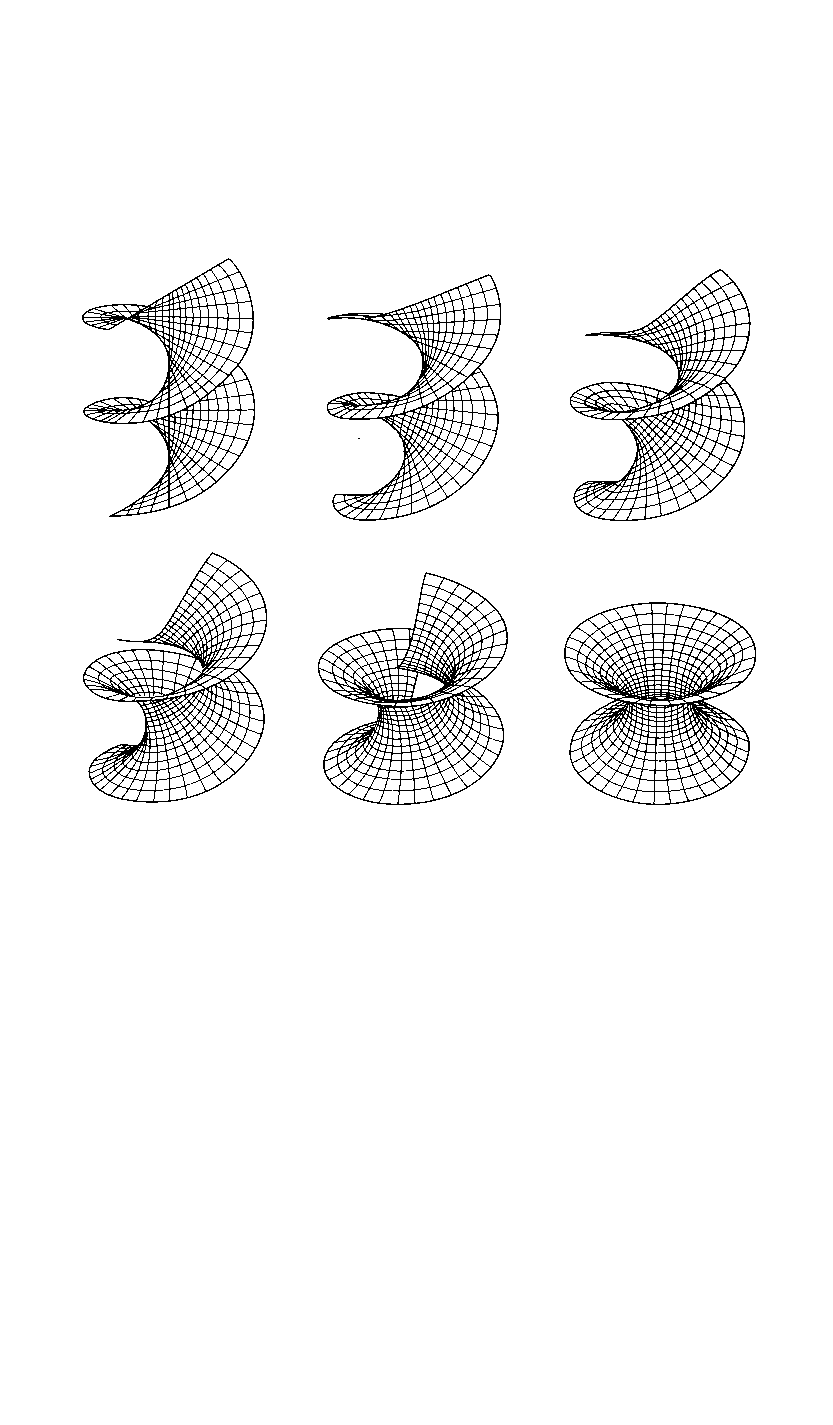
\includegraphics[scale=0.5]{figures/helicoid.pdf}
    \caption{A $1$-parameter family of minimal ($H=0$) isometric immersions of a surface connecting the helicoid (top left) to the catenoid (bottom right). From \cite{Spivak3}.}
    \label{fig:helicoid}
\end{figure}

\begin{example}[Helicoid]\label{ex helicoid}
    Let $a>0$ be a constant and consider the following map $\bf{x}:\bbR^2\to \bbR^3$:
    \[\bf{x}(s,t)=(s\cos t,s\sin t,at).\]
    Its image is called the \emph{helicoid}.\index{Helicoid} Note that the $z$-axis is contained in the surface, as is a horizontal line emanating out of each point on the $z$-axis, and this line rotates as we move up the $z$-axis.
    
    We now compute the first-order adapted frame $\frake:\bbR^2\to \bbE^3$ for the helicoid (as usual, we identify the surface with its domain in $\bbR^2$ under the parametrization). Note that 
    \begin{align}
        \bf{x}_s&=(\cos t,\sin t,0),\\
        \bf{x}_t&=(-s\sin t,s\cos t,a),
    \end{align}
    so $\bf{x}_s\perp \bf{x}_t$ and we may take 
    \begin{align}
        e_1&=\frac{\bf{x}_s}{\lVert\bf{x}_s\rVert}=(\cos t,\sin t,0), \notag\\
        e_2&=\frac{\bf{x}_t}{\lVert\bf{x}_t\rVert}=\frac{1}{\sqrt{s^2+a^2}}(-s\sin t,s\cos t,a),\label{eq 2.7 Ivey}\\
        e_3&=e_1\times e_2=\frac{1}{\sqrt{s^2+a^2}}(a\sin t,-a\cos t,s).\notag
    \end{align}
    Since $\dd\bf{x}=\bf{x}_s\dd s+\bf{x}_t\dd t=\frake^\ast(\theta^1)e_1+\frake^\ast(\theta^2)e_2$, we obtain (omitting $\frake^\ast$ from the notation from now on)
    \[\theta^1=\dd s,\quad \theta^2=\sqrt{s^2+a^2} \dd t.\label{eq 2.8 Ivey}\]
    Next, we calculate the Gauss map:
    \begin{multline}
        \dd e_3=\left(-s\left(s^2+a^2\right)^{-3/2}(a\sin t,-a\cos t,s)+(s^2+a^2)^{-1/2}(0,0,1)\right)\dd s+\\
        +(s^2+a^2)^{-1/2}(a\cos t,a\sin t,0)\dd t.
    \end{multline}
    So, using \eqref{eq 2.7 Ivey} and \eqref{eq 2.8 Ivey}, we obtain 
    \[\omega_1^3=-a(s^2+a^2)^{-1}\theta^2,\quad \omega_2^3=-a(s^2+a^2)^{-1}\theta^1.\]
    The coefficients in front of $\theta^i$ are the principal curvatures $k_i$. We conclude that $H(s,t)=0$ and $K(s,t)=-\frac{a^2}{(s^2+a^2)^2}$. Thus, the helicoid is a umbilic-free minimal surface.
\end{example}

Being a union of disjoint straight lines, the helicoid is an example of a \emph{ruled} surface.

\begin{defn}[Flat, ruled, tangential developable surfaces]\index{Developable surface|see {Flat surface}}\index{Ruled surface}\index{Tangential surface}\index{Flat surface}
    A surface is called \emph{developable}, or simply \emph{flat}, if its Gauss curvature vanishes everywhere, $K\equiv 0$.

    A surface is called \emph{ruled} if every point of the surface is contained in it along with a segment of a straight line passing through that point, whose ends (if they exist) lie on the boundary of the surface.

    In particular, a surface $\varSigma\subset\bbE^3$ is said to be \emph{tangential developable} if it can be described as (a subset of) the union of tangent rays to a curve. (These surfaces are also called \emph{tangential surfaces}.)
\end{defn}
The following proposition clarifies what tangential surfaces look like.
\begin{prop}
    Let $\gamma:\bbR\to \bbE^3$ be a regular parametrized curve with curvature and torsion $\kappa$ and $\tau$, respectively, and consider the tangential surface $\bf{x}:\bbR\times \bbR_+\to \bbE^3$ defined by 
    \[\bf{x}:(u,v)\mapsto \gamma(u)+v\dot\gamma(u),\quad v>0.\]
    Then this surface has $H(u,v)=\frac{\tau(u)}{2\kappa(u)v}$ and $K\equiv 0$.
\end{prop}
\begin{proof}
    Since 
    \[\dd \bf{x}=(\dot\gamma(u)+v\ddot\gamma(u))\dd u+\dot\gamma(u)\dd v,\]
    we see that $\bf{x}$ is regular, i.e., $\dd f$ is of maximal rank, when $\ddot \gamma(u)$ is linearly independent from $\dot\gamma(u)$ and $v\neq 0$, i.e., exactly when $\gamma$ is regular. Now assume that $\gamma$ is parametrized by arclength. Then $\dot\gamma\perp\ddot\gamma$ and we can take $e_1(u,v)=\dot\gamma(u)$ and $e_2(u,v)=\ddot\gamma(u)/\lVert\ddot\gamma(u)\rVert$. Using $\dd \bf{x}=\theta^1e_1+\theta^2e_2$, we calculate 
    \[\theta^1=\dd u+\dd v,\quad \theta^2=v\kappa(u)\dd u.\]
    Note that this frame coincides with the Frenet frame of $\gamma$, so, following Example~\ref{ex serret-frenet}, we have 
    \[\dd e_3=-\tau(u)e_2\dd u.\]
    Therefore, 
    \[\omega_1^3=0,\quad \omega_2^3=\frac{\tau(u)}{\kappa(u)v}\theta^2,\]
    which leads to the asserted $H$ and $K$.
\end{proof}

\begin{rem}
    Not every ruled surface is flat (consider a single-sheet hyperboloid or the hyperbolic paraboloid $z=xy$ in $\bbR^3$). However, the converse does hold (aside from degenerate cases): if a given immersed surface has $K\equiv 0$, then one of the principal curvatures must be zero. Assume the other one isn't. Since line of curvature coordinates exist (see Example~\ref{ex Gauss curvature in orthogonal coords}), one of these coordinates, say $v$, will generate straight lines in $\varSigma$, making it ruled. The surface has to locally lie on one side of its tangent planes containing the $v$-lines and include the entire segments of these lines up to its boundary, otherwise the ends of the segment would be points of positive curvature. In summary, a surface is ruled iff it is flat. Hence, flat surfaces are identified with (pieces of) ``flat sheets of paper'' arbitrarily bent in $3$-dimensional space without stretching. 
    
    Note that these statements are particular to $3$ dimensions and fail already in $\bbE^4$ where, for example, the flat torus $\bbT^2$ can be isometrically embedded, whereas it is obviously not ruled by virtue of being compact with no boundary.
\end{rem}


\begin{example}[Catenoid]\label{ex catenoid}
    Let $a>0$ be a constant and consider the following map $\bf{x}:\bbR^2\to \bbR^3$:
    \[\bf{x}(u,v)=(a\cosh v\cos u,a\cosh v\sin u,av).\]
    Its image is called the \emph{catenoid}.\index{Catenoid}
    By choosing an adapted frame and differentiating one can compute that $H=0$, so this is a minimal surface. Now consider the map $f:\bbR^2\to \bbR^2$ given by
    \[f: (u,v)\mapsto (s,t)=(a\sinh v,u).\]
    One then shows that $f^\ast(K_{\mathrm{helicoid}})=K_{\mathrm{catenoid}}$, and of course the mean curvatures match as well. But while these two surfaces have the same $H$ and $K$, the helicoid is ruled, whereas the catenoid contains no line segments. Thus, they are not congruent.
\end{example}

Nevertheless, $H$ and $K$ are usually sufficient to determine $\varSigma$ up to congruence. Those surfaces for which this is not the case either have constant $H$ or belong to a finite-dimensional family called \emph{Bonnet surfaces}.

\begin{xca}
    A surface $\varSigma$ is called \emph{flat} if $K\equiv 0$. Show that if $\varSigma$ is flat, there exist local coordinates $x^1,x^2$ on it and an orthonormal frame $(e_1,e_2,e_3)$ such that $\theta^1=\dd x^1$, $\theta^2=\dd x^2$.
\end{xca}





\section{Codazzi equation}

Let us now derive the compatibility condition on $\sfh$ by setting up a Pfaffian system. Treat $\{h_{11},h_{12},h_{22}\}$ as coordinates in $\bigodot\nolimits^2 \bbR^2\cong\bbR^3$ and define an \gls{eds} $\calI\subset \Omega^{\smbullet }(\SE_3\times \bbR^3)$ by
\[\calI\coloneqq \<\theta^3,\omega_1^3-h_{11}\theta^1-h_{12}\theta^2,\omega_2^3-h_{12}\theta^1-h_{22}\theta^2\>_{\mathrm{diff}}\]
with independence condition $\theta^1\wedge\theta^2\neq 0$.
From our above computations, we know that along the lifting of any hypothetical surface $\varSigma$, this entire \gls{eds} must vanish. The independence condition means that $\theta^1\wedge\theta^2$ must produce a volume form after pullback to $\varSigma$. The integral manifolds of this system are graphs of immersions $\restr{P}{U}\to \SE_3$ that are adapted frame bundles of isometric immersions $\bf{x}:U\to \bbE^3$ satisfying $\bf{x}^\ast \sfI=\sfg$ and $\bf{x}^\ast \wt{Q}=\sfh$. By the Frobenius Theorem~\ref{thm 4.7.8 RS1}, the derivatives of the generators of $\calI$ must vanish modulo $\calI$ on $\varSigma$. First, it is easy to check that $\dd\theta^3\equiv 0 \pmod{\calI}$. The differentials of the other two forms can be combined into a column-vector and rewritten modulo $\calI$ using the definition of $\sfh$:
\begin{multline}
    \dd \left\{
        \begin{pmatrix}
            \omega_1^3\\\omega_2^3
        \end{pmatrix}
        -\sfh\cdot 
        \begin{pmatrix}
            \theta^1\\\theta^2
        \end{pmatrix}
    \right\}=\\
    =-\begin{pmatrix}
        0&-\omega_1^2\\
        \omega_1^2& 0
    \end{pmatrix}\wedge 
    \begin{pmatrix}
        \omega_1^3\\\omega_2^3
    \end{pmatrix}
    -\dd \sfh\wedge 
    \begin{pmatrix}
        \theta^1\\\theta^2
    \end{pmatrix}
    +\sfh \cdot\begin{pmatrix}
        0&-\omega_1^2\\
        \omega_1^2& 0
    \end{pmatrix}\wedge 
    \begin{pmatrix}
        \theta^1\\\theta^2
    \end{pmatrix} \equiv 
    \\
    \equiv
    -\begin{pmatrix}
        0&-\omega_1^2\\
        \omega_1^2& 0
    \end{pmatrix}\wedge \sfh\cdot
    \begin{pmatrix}
        \theta^1 \\ \theta^2
    \end{pmatrix}
    -\dd \sfh\wedge 
    \begin{pmatrix}
        \theta^1\\\theta^2
    \end{pmatrix}
    +\sfh\cdot \begin{pmatrix}
        0&-\omega_1^2\\
        \omega_1^2& 0
    \end{pmatrix}\wedge 
    \begin{pmatrix}
        \theta^1\\\theta^2
    \end{pmatrix}\pmod{\calI}.\label{eq I^1_taut structure}
\end{multline}
These derivatives must vanish along the integral manifolds. Thus, $\sfh$ must satisfy the \emph{Codazzi-Mainardi equation},\index{Equation!Codazzi-Mainardi} which we will call the Codazzi equation:
\[\boxed{\left\{\dd \sfh+\left[
\begin{pmatrix}
    0 & -\omega_1^2\\
    \omega_1^2 & 0
\end{pmatrix},\sfh
\right]\right\} \wedge 
\begin{pmatrix}
    \theta^1\\\theta^2
\end{pmatrix}=0,}\label{eq Gauss-Codazzi}
\]
where $[\,,\,]$ is the commutator of matrices. (Note that in this equation a pullback to the adapted frame bundle of a surface is implied, otherwise it holds only modulo $\calI$.)

The proof of Gauss' Theorema Egregium~\ref{thm egregium} showed that, given a metric $\sfg$ on $\varSigma$ and an orthonormal frame $\frake$, $\frake^\ast \omega_1^2$ is uniquely determined. Thus, \eqref{eq Gauss-Codazzi} is a system of equations for the possible fundamental forms $\sfII=h_{ij}\theta^i\otimes \theta^j\otimes e_3$ for embdeddings of $\varSigma$ into $\bbE^3$ that induce the metric $\sfg$. These equations are well-defined, since \eqref{eq Gauss-Codazzi} is invariant under changes of the frame $\frake$. Thus, the Frobenius theorem guarantees existence, while uniqueness up to a rigid motion is guaranteed only for a fixed parametrization.

\begin{thm}[Bonnet's Fundamental Theorem of Surfaces]\index{Theorem!Bonnet's Fundamental Theorem}
    Let $U$ be an open domain in $\bbR^2$. Two parametric surfaces $\bf{x},\wt{\bf{x}}:U\to \bbE^3$ are congruent (via an element of $\SE_3$) iff they have the same first and second fundamental forms at corresponding points:
    \[\bf{x}^\ast\sfI=\wt{\bf{x}}^\ast \wt{\sfI},\quad \bf{x}^\ast\sfII=\wt{\bf{x}}^\ast \wt{\sfII}.\] 
    Moreover, if $\sfg$ and $\sfh$ are given quadratic forms on $U$ satisfying the Gauss-Codazzi equations with $\sfg$ positive definite, then there exists an immersion $\bf{x}:U\to \bbE^3$ such that $\bf{x}^\ast  \sfI=\sfg$ and $\bf{x}^\ast  \wt{Q}=\sfh$.
\end{thm}
Note that the immersion $\bf{x}$ needs to be specified to claim uniqueness up to congruence. If only $K$ and $H$ are given, the surface cannot be reconstructed uniquely, as we saw above.
\begin{proof}
    First we show uniqueness. Let $\bf{x}:U\to \bbE^3$ be given. Then, by following the above construction, we define the adapted frame bundle $\pi:P\to U$ consisting of triples $(p,e_1,e_2)$ where $(e_1,e_2)$ are $\sfI$-orthonormal bases for $\T_p U$. There are unique $1$-forms $\theta^1,\theta^2,\omega_1^2$ such that 
    \[\pi_\ast(X)=e_1\theta^1(X)+e_2\theta^2(X),\quad X\in \T_{(p,e_1,e_2)}P,\]
    and
    \[\dd\theta^1=\omega_1^2\wedge \theta^2,\quad \dd\theta^2=-\omega_1^2\wedge\theta^1.\]
    Then 
    \[\pi^\ast\sfI=\sum_{\mu=1}^2\theta^\mu\otimes\theta^\mu,\quad \pi^\ast \wt{Q}=\sum_{\mu,\nu=1}^2 h_{\mu\nu}\theta^\mu\otimes\theta^\nu\]
    with some uniquely determined functions $h_{\mu\nu}$ such that $h_{12}=h_{21}$. Now we define $\omega_1^3\coloneqq h_{11}\theta^1+h_{12}\theta^2$ and $\omega_2^3\coloneqq h_{12}\theta^1+h_{22}\theta^2$. Then, as we saw above, $\frake\coloneqq(\bf{x}_u,\bf{x}_v,\bf{x}_u\times \bf{x}_v)$ must satisfy 
    \[\dd \begin{pmatrix}
        \frake & \bf{x}\\
        0& 1
    \end{pmatrix}=\begin{pmatrix}
        \frake & \bf{x}\\
        0& 1
    \end{pmatrix}
    \begin{pmatrix}
        0 & -\omega_1^2 & -\omega_1^3& \theta^1\\
        \omega_1^2 & 0 & -\omega_2^3 & \theta^2\\
        \omega_1^3 & \omega_2^3 & 0 & 0\\
        0 & 0& 0& 0
    \end{pmatrix}.
    \]
    Then the $4\times 4$ matrix on the right takes values in the Lie algebra $\frakse_3$, and Cartan's Fundamental Theorem~\ref{thm 6.1 Sharpe fundamental local} guarantees the uniqueness of the map $\left(\begin{smallmatrix}
        \frake & \bf{x}\\
        0& 1
    \end{smallmatrix}\right): U\to \SE_3$ up to a left multiplication by an element of $\SE_3$, which is what a congruence is.

    Existence follows from the existence part of Cartan's Fundamental Theorem, since the Gauss-Codazzi equations are equivalent to the structure equation for the function $\left(\begin{smallmatrix}
        \frake & \bf{x}\\
        0& 1
    \end{smallmatrix}\right)$.
\end{proof}

\begin{rem}
    We can put the Gauss-Codazzi equations in an even more suggestive form by splitting up the components of all objects into tangent and normal to $\varSigma$. Let Greek indices range only over tangent directions ($1,2$), and this time we will be careful to put the row (top) index before the column (bottom) index in $\omega^i{}_j$. Then we have the two defining equations on the adapted frame bundle $P$:
    \[\dd e_\mu=e_3\omega^3{}_\mu + e_\nu\omega^\nu{}_\mu,\quad \dd e_3=e_\mu\omega^\mu{}_3.\]
    By definition of $h$ \eqref{def h}, we have $\omega^3_\mu=h_{\mu\nu}\omega^\nu$, and therefore the system becomes 
    \[\dd e_\mu= e_3 h_{\mu\nu}\omega^\nu+ e_\nu\omega^\nu{}_\mu ,\quad \dd e_3=e_\mu\omega^\mu{}_3.\]
    The Frobenius compatibility conditions for these two equations are $\dd^2 e_\mu=0$ and $\dd^2 e_3=0$. We expand the first one, use $\dd e_3=e_\mu\omega^\mu{}_3$, and collect terms containing the same basis vector:
    \[0=\dd^2e_\mu=e_3\left(\dd \omega^3{}_\mu-\omega^\nu{}_\mu\wedge\omega^3{}_\nu\right)
    +e_\nu\left(\dd\omega^\nu{}_\mu+\omega^\nu{}_\lambda\wedge\omega^\lambda{}_\mu+\omega^\nu{}_3\wedge\omega^3{}_\mu\right),
    \]
    which is equivalent to the pair of equations 
    \begin{align}
        \dd\omega^3{}_\mu-\omega^\lambda{}_\mu\wedge\omega^3{}_\lambda&=0,\\
        \dd\omega^\nu{}_\mu-\omega^\lambda{}_\mu\wedge\omega^\nu{}_\lambda&=-\omega^\nu{}_3\wedge \omega^3{}_\mu.
    \end{align}
    It is easy to check that these equations also imply the second compatibility condition, $\dd^2 e_3=0$. 
    
    By putting $b_\mu\coloneqq \omega^3{}_\mu=-\omega^\mu{}_3\eqqcolon-b^\mu$ and $\varGamma^\nu{}_\mu\coloneqq \omega^\nu{}_\mu$, we get the defining equations
    \[\begin{cases}
        \dd e_\mu=b_\mu e_3+\varGamma^\nu{}_\mu e_\nu, &\\
        \dd e_3=b^\mu e_\mu, &\text{(Weingarten)}
    \end{cases}\label{3791}\]
    and the compatibility conditions for them are
    \begin{align}
        \dd b_\mu-\varGamma^\lambda{}_\mu \wedge b_\lambda&=0 &\text{(Codazzi),}\\
        \dd \varGamma^\nu{}_\mu-\varGamma^\lambda{}_\mu\wedge\varGamma^\nu{}_\lambda&=-b^\nu\wedge b_\mu &\text{(Gauss).}
    \end{align}
    Note that the right hand side of the Gauss equation is exactly $K \omega^\nu\wedge\omega^\mu$ since $b_\mu=h_{\mu\nu}\omega^\nu$ and $K=\det h$. Thus, if these Gauss-Codazzi equations are satisfied by the second fundamental form $b_\mu$, then the defining equations \eqref{3791} can be uniquely solved for $(e_1,e_2,e_3)$ (with some initial condition), providing a map into the orthonormal frame bundle over $\bbE^3$, and hence an isometric immersion into $\bbE^3$. In time we will identify $\varGamma^\nu{}_\mu$ with the components of a (Levi-Civita) connection on the surface and $b_\mu$ with the components of a connection on its normal bundle.
\end{rem}




\section{\texorpdfstring{\gls{eds}}{EDS} for surfaces}


In this \sect\ we put the above discussion in terms of the theory of \glspl{eds} developed in the preceding \chap, and consider some related examples of geometric \glspl{eds}. First let us define the simple \emph{tautological} \gls{eds} for immersed surfaces in $\bbE^3$. This is the Pfaffian system on the orthonormal bundle $\SE_3$ generated by the single form $\theta^3$:
\[\calI_{\mathrm{taut}}=\<\theta^3\>_{\mathrm{diff}}.\]
Any $2$-dimensional integral manifold is locally described by some function $(\bf{x},\frake)$, where $\frake$ is an orthonormal frame at $\bf{x}$. The vanishing of $\theta^3$ along the integral manifolds implies that $\dd \bf{x}=e_1\theta^1+e_2\theta^2$, which is exactly the statement that the image of $(\bf{x},\frake)$ is consists of first-order adapted frames of the surface parametrized by $\bf{x}$. Thus, $3$-dimensional integral manifolds of this system are exactly the bundles of adapted frames of immersed surfaces. The following example establishes that this system is not involutive.

\begin{example}[Involutivity of $\calI_{\mathrm{taut}}$]
    The structure equation is $\dd\theta^3=\omega^3_i\wedge\dd\theta^i$, so $(s_1,s_2,s_3)=(1,0,0)$. A coframe for a bundle of adapted frames is given by $\theta^1,\theta^2,\omega^2_1$, and the remaining directions on $\SE_3$ are $\omega^3_1,\omega^3_2,\theta^3$. Thus, integral elements are parametrized by linear equations of the form 
    \[
    \begin{pmatrix}
        \omega^3_1\\
        \omega^3_2\\
        \theta^3
    \end{pmatrix}=
    \begin{pmatrix}
        a & b & e \\
        c & d & f \\
        0 & 0 & 0
    \end{pmatrix}
    \begin{pmatrix}
        \theta^1\\\theta^2\\\omega^2_1
    \end{pmatrix},
    \]
    subject to $0=\dd\theta^3=(b-c)\theta^1\wedge\theta^2+e\omega^2_1\wedge\theta^1+f\omega^2_1\wedge\theta^2$, so $b=c$ and $e=f=0$. Thus, the space of $3$-dimensional integral elements at a point is of dimension $3$, and $3>s_1+2s_2+3s_3=1$, so the system is not involutive.
\end{example}

Another way to see that this system is not involutive is to notice that it has a Cauchy characteristic that corresponds to locally rotating the tangent frames $(e_1,e_2)$. In other words, the system has an angular ``dummy variable'' whose presence forbids the uniqueness of integral manifolds, necessary for the Cartan-K\"ahler Theorem to work. The following example shows this in detail.

\begin{example}[Cauchy characteristics of $\calI_{\mathrm{taut}}$]\label{ex 7.1.10 Ivey}
    The system $\calI_{\mathrm{taut}}$ admits a Cauchy characteristic vector field as follows.

    Let $\{E_j,E^i_j\}$ be a global frame for $\T P$ dual to the one given by the entries of the Maurer-Cartan form $\{\theta^j,\omega^i_j\}$. Expand $X=X^jE_j+X^j_i E^i_j$. Then $i_X\theta^3=0$ implies that $X_3=0$ and 
    \[i_X \dd\theta^3=i_X(-\omega^3_1\wedge\theta^1-\omega^3_2\wedge\theta^2)=X_1\omega^3_1-X^1_3\theta^1+X_2\omega^3_2-X^2_3\theta^2\]
    implies that $X=X^1_2 E^2_1$. We can pick $X=E^2_1$, which generates rotations of the frame in the $\{e_1,e_2\}$-plane. Now, Proposition~\ref{prop 7.1.8 Ivey} implies that any integral surface for $\calI$ may be ``thickened'' to an integral $3$-manifold using the Cauchy characteristic.

    Now, $\calC(\calI)$ is the Frobenius system on $\SE_3$ spanned by $\theta^1,\theta^2,\theta^3,\omega^3_1,\omega^3_2$. Integral curves of $\calC(\calI)$ form a foliation of $\SE_3$. The leaf space for this foliation is a 5-dimensional homogeneous space which we identify with $\bbS(\T\bbE^3)$, the unit sphere bundle of the tangent bundle of $\bbE^3$, by letting $m$ be the basepoint and $e_3$ the unit vector in $\T_m\bbE^3$.\index{Sphere bundle}
\end{example}

The surface $\varSigma$ can be described by the restrictions of the forms $\theta^1,\theta^2$ to its bundle of adapted frames $P\subset \SE_3$. To find out whether these data are sufficient to recover the shape of $\varSigma$, it makes sense to set up another \gls{eds} $\calI_\varSigma$ on $P\times\SE_3$ that \emph{compares} two different sets of forms, namely the Pfaffian system generated by the $1$-forms 
\[\begin{pmatrix}
    \vartheta_1\\\vartheta_2\\\vartheta_3
\end{pmatrix}\coloneqq 
\begin{pmatrix}
    \wt\theta^1-\theta^1\\
    \wt\theta^2-\theta^2\\
    \wt\theta^3
\end{pmatrix},
\]
where $\wt\theta^i$ are the standard forms on $\SE_3$ and $\theta^i$ are the fixed forms on $P$ (we omit pullbacks of both to $P\times\SE_3$). Along $P$, all of these forms vanish, while the $1$-forms $\theta^1,\theta^2,\omega^2_1$ form a coframe. Conversely, we will eventually prove that all integral manifolds with this coframe are locally frame bundles of isometric immersions of $\varSigma$. For the moment, we concentrate on asking whether we can apply the Cartan-K\"ahler Theorem.

\begin{example}[Cartan's Test for $\calI_\varSigma$]
    First we compute the tableau:
    \[\dd \begin{pmatrix}
        \vartheta_1\\\vartheta_2\\\vartheta_3
    \end{pmatrix}
    =-\begin{pmatrix}
        0 & \wt\omega^2_1-\omega^2_1 & 0\\
        \boxed{-(\wt\omega^2_1-\omega^2_1)} & 0 & 0\\
        \boxed{\wt\omega^3_1} & \boxed{\wt\omega^3_2} & 0
    \end{pmatrix}\wedge 
    \begin{pmatrix}
        \vartheta_1\\\vartheta_2\\\vartheta_3
    \end{pmatrix} \pmod{\vartheta^1,\vartheta^2,\vartheta^3}.
    \]
    We have $(s_1,s_2,s_3)=(2,1,0)$. Each $3$-dimensional integral element has $\wt\theta^i=\theta^i$, so is determined by the linear equations relating $\wt\omega^i_j$ to $\theta^1,\theta^2,\omega^2_1$ such that $\dd\vartheta^i=0$:
    \[\begin{pmatrix}
        \wt\omega^3_1\\
        \wt\omega^3_2\\
        \wt\omega^2_1-\omega^2_1
    \end{pmatrix}=
    \begin{pmatrix}
        \wt h_{11} & \wt h_{12} & 0\\
        \wt h_{12} & \wt h_{22} & 0\\
        0 & 0 & 0
    \end{pmatrix}
    \begin{pmatrix}
        \theta^1\\\theta^2\\\omega^2_1
    \end{pmatrix}.\label{eq 12942}
    \]
    Therefore, there is a $3$-dimensional space of integal elements at each point. But $s_1+2s_2=4>3$, so involution fails and we can't apply the Cartan-K\"aher Theorem, and prolongation is necessary. Another way to see this is to check whether the generic integral line sits in an integral plane. The equations on integral lines are $\wt\theta^1=\theta^1$, $\wt\theta^2=\theta^2$, $\wt\theta^3=0$. On any integral plane $\wt\omega^2_1=\omega^2_1$. The generic integral line does not sit in an integral plane because it doesn't have to satisfy $\wt\omega^2_1=\omega^2_1$.
\end{example}

The procedure in the last \sect\ where we adjoined the Second Fundamental Form to the system as an independent variable is in fact exactly the \emph{first prolongation} of $\calI_{\mathrm{taut}}$. We also call the resulting system the tautological system on $\SE_3\times\bbR^3_{h_{ij}}$ for surfaces in $\bbE^3$. The integral manifolds of this system are still the first-order adapted lifts of arbitrary surfaces in $\bbR^3$, together with the components of the second fundamental form $\{h_{ij}\}$, which we view as coordinates of another space $\bbR^3$. This Pfaffian system $\calI^{(1)}_{\mathrm{taut}}=\<I\>_{\mathrm{diff}}$ is generated by 
\[\begin{pmatrix}
    \vartheta^1\\
    \vartheta^2\\
    \vartheta^3
\end{pmatrix}=
\begin{pmatrix}
    \omega^3_1-h_{1\mu}\theta^\mu\\
    \omega^3_2-h_{2\mu}\theta^\mu\\
    \theta^3
\end{pmatrix}.\]
The next example directly verifies, for this particular system, the by now familiar fact that the prolongation of an involutive system is involutive. 

\begin{example}[Involutivity of $\calI^{(1)}_{\mathrm{taut}}$]
    Then \eqref{eq I^1_taut structure} reads
    \begin{align}
        \dd \begin{pmatrix}
            \vartheta^1\\
            \vartheta^2\\
            \vartheta^3
        \end{pmatrix}
        \equiv& \begin{pmatrix}
            2h_{12}\omega^2_1-\dd h_{11} & (h_{22}-h_{11})\omega^2_1-\dd  h_{11}\\
            (h_{22}-h_{11})\omega^2_1-\dd h_{12} & -2h_{12}\omega^2_1-\dd h_{22}\\
            0 & 0\\
        \end{pmatrix}\wedge 
        \begin{pmatrix}
            \theta^1\\
            \theta^2
        \end{pmatrix}\pmod{I} \notag \\
        \eqqcolon& 
        \begin{pmatrix}
            \pi^1_1 & \pi^1_2\\
            \pi^2_1 & \pi^2_2\\
            \pi^3_1 & \pi^3_2
        \end{pmatrix}\wedge 
        \begin{pmatrix}
            \theta^1\\
            \theta^2
        \end{pmatrix}\pmod{I}.
    \end{align}
    The symbol relations are 
    \[\pi^3_1\equiv \pi^3_2\equiv \pi^2_1-\pi^1_2\equiv 0\pmod{I}.\]
    There is no intrinsic torsion, and $(s_1,s_2)=(2,1)$. Integral elements are given by 
    \begin{align}
        \pi^1_1&=a\theta^1+b\theta^2,\notag\\
        \pi^1_2&=\pi^2_1=b\theta^1+c\theta^2,\notag\\
        \pi^2_2&=c\theta^1+e\theta^2,\notag\\
        \pi^3_1&=\pi^3_2=0,
    \end{align}
    where $a,b,c,e$ are arbitrary. Thus, $\dim A^{(1)}=4=s_1+2s_2$, and the system is involutive. The Cartan-K\"ahler Theorem implies that integral manifolds depend on one function of two variables. This is expected since locally any surface is a graph of a function $z=f(x,y)$. 
    
    Finally, we observe that the Codazzi equation is exactly the structure equation for this system pulled back to an integral surface, and the Gauss equation is similarly the pullback of $\dd\omega^2_1\equiv- K\theta^1\wedge\theta^2\pmod{\calI_{\mathrm{taut}}^{(1)}}$.
\end{example}

Finally, to compute the differential invariants of $\varSigma$, we should prolong $\calI_\varSigma$ and check involutivity. This means that we need to treat $\wt{h}_{ij}$ as new independent variables and turn \eqref{eq 12942} into the condition for the vanishing of three new generating $1$-forms:
\[
    \begin{pmatrix}
        \vartheta_4\\
        \vartheta_5\\
        \vartheta_6
    \end{pmatrix}\coloneqq 
    \begin{pmatrix}
        \wt\omega^3_1\\
        \wt\omega^3_2\\
        \wt\omega^2_1-\omega^2_1
    \end{pmatrix}=
    \begin{pmatrix}
        \wt h_{11} & \wt h_{12} & 0\\
        \wt h_{12} & \wt h_{22} & 0\\
        0 & 0 & 0
    \end{pmatrix}
    \begin{pmatrix}
        \theta^1\\\theta^2\\\omega^2_1
    \end{pmatrix}.
\]
Note that $\dd\vartheta_i\equiv 0\pmod{\vartheta_4,\vartheta_5,\vartheta_6}$ for $i=1,2,3$, so we can omit them in the analysis. 
\[\dd \begin{pmatrix}
    \vartheta_4\\
    \vartheta_5\\
    \vartheta_6
\end{pmatrix} \equiv 
-\begin{pmatrix}
    \boxed{D\wt{h}_{11}} & D\wt{h}_{12} & 0\\
    \boxed{D\wt{h}_{12}} & \boxed{D\wt{h}_{22}} & 0\\
    0 & 0 & 0
\end{pmatrix}\wedge 
\begin{pmatrix}
    \theta^1\\\theta^2\\\omega^2_1
\end{pmatrix}
+\begin{pmatrix}
    0 \\ 0\\ t\theta^1\wedge\theta^2
\end{pmatrix}\pmod{\vartheta_1,\ldots,\vartheta_6},
\]
where 
\[\begin{pmatrix}
    D\wt{h}_{11}\\
    D\wt{h}_{12}\\
    D\wt{h}_{22}
\end{pmatrix}
\coloneqq 
\begin{pmatrix}
    \dd\wt{h}_{11} +2\wt{h}_{12}\omega^2_1+a \theta^1+b\theta^2\\
    \dd\wt{h}_{12}+(\wt{h}_{11}-\wt{h}_{22})\omega^2_1+b\theta^1+c\theta^2\\
    \dd\wt{h}_{22}+2\wt{h}_{12}\omega^2_1+c\theta^1+d\theta^2
\end{pmatrix},
\]
with $a,b,c,d$ arbitrary, and the torsion is 
\[t\coloneqq \det \wt{h}-\det h=\det\wt h-K.\]
This torsion clearly has to vanish on any $3$-dimensional integral element of $\calI^{(1)}_\varSigma$, i.e., every such element lives over the subset of $M=P\times\SE_3$ on which $K=\det\wt h$. To ensure that this subset is a submanifold, we let $M'\subset M$ be the set of points where this equation is satisfied and at least one of $\wt{h}_{ij}$ is not zero. Clearly $M'\subset M$ is a submanifold, on which we find $D\wt h_{ij}$ linearly independent. On $M'$ we have
\[
    \dd \begin{pmatrix}
        \vartheta_4\\
        \vartheta_5\\
        \vartheta_6
    \end{pmatrix} \equiv 
    -\begin{pmatrix}
        \boxed{D\wt{h}_{11}} & D\wt{h}_{12} & 0\\
        \boxed{D\wt{h}_{12}} & D\wt{h}_{22} & 0\\
        0 & 0 & 0
    \end{pmatrix}\wedge 
    \begin{pmatrix}
        \theta^1\\\theta^2\\\omega^2_1
    \end{pmatrix}\pmod{\vartheta_1,\ldots,\vartheta_6},
\]
so $(s_1,s_2,s_3)=(2,0,0)$. There are $2$ dimensions of integral elements (down from $3$ due to Gauss' equation $K=\det\wt{h}_{ij}$), so we have involution. This confirms again that $\wt{h}$ contains the full set of differential invariants.

The next two examples are adapted from Cartan's 1945 treatise \cite{cartan45}.
\begin{example}[Linear Weingarten surfaces]\label{ex Weingarten surfaces}
    Let $A,B,C\in\bbR$ with $A\neq 0$, and let $AK+2BH+C=0$ be a linear relation between functions $H,K$. We will now set up the space of general integral manifolds for first-order adapted liftings of surfaces in $\bbR^3$, together with the components of the second fundamental form, having Gauss and mean curvatures satisfying this relation.

    This is the system above restricted to a codimension one submanifold $M\subset \SE_3\times \bbR^3_{h_{ij}}$. The submanifold is defined by the equation 
    \[A(h_{11}h_{22}-h_{12}^2)+B(h_{11}+h_{22})+C=0.\]
    The differential of this equation implies that on $M$ we may write 
    \[\dd h_{12}=\alpha d h_{11}+\beta dh_{22}\]
    for some functions $\alpha,\beta$, and thus 
    \[\pi^1_2=\alpha\pi^1_1+\beta\pi^2_2.\]
    We still have no intrinsic torsion and have characters $(s_1,s_2)=(2,0)$.  This is automatically involutive because any tableau with characters $(s_1,\ldots,s_{n-1},s_n)=(s,\ldots,s,0)$, where $s=\dim W$, is involutive. Solutions depend on two functions of one variable. This suggests that an appropriate Cauchy problem for determining such surfaces would be to start out with a space curve (the two functions being its curvature and torsion) and then solve for a unique surface containing the curve. Cartan carries out this construction explicitly in his treatise \emph{Les Syst\`emes Ext\'erieurs et leurs Applications G\'eom\'etriques}.
\end{example} 

\begin{example}[Conformally equivalent surfaces]
    Let $(\varSigma,\sfg)$ and $(\wb\varSigma,\wb \sfg)$ be analytic Riemannian surfaces. We set up and solve the \gls{eds} for maps $\phi:\varSigma\to \wb \varSigma$ that preserve the metric up to (point-dependent) scale, i.e., for \emph{conformal} maps.

    Let $P=\Fr_{\SO_2}(\T^\ast \varSigma)$ denote the orthonormal coframe bundle of $\varSigma$, with coframe $\{\theta^1,\theta^2,\omega^2_1=-\omega^1_2\}$ satisfying $\dd\theta^i=-\omega^i_j\wedge \theta^j$ as usual. Similarly, let $\wb P$ denote the orthonormal coframe bundle of $\wb\varSigma$ with coframe $\{\wb\theta^1,\wb\theta^2,\wb\omega^2_1\}$. The metric on $\varSigma$ is given by the pullback of $(\theta^1)^2+(\theta^2)^2$ (tensor squares) along any section $s:\varSigma\to P$, and that on $\wb P$ by the pullback of $(\wb\theta^1)^2+(\wb\theta^2)^2$. Thus, a conformal map $\phi:\varSigma\to \wb\varSigma$ induces  a map $\varPhi:P\to \wb P$ such that $\varPhi^\ast \left((\wb\theta^1)^2+(\wb\theta^2)^2\right)=\lambda^2 \left((\theta^1)^2+(\theta^2)^2\right)$ for some positive function $\lambda>0$.

    \gls{wlog}, we may require that $\varPhi^\ast\theta^j=\lambda\omega^j$ because we have freedom to rotate in the tangent spaces at each point. So on $M\coloneqq P\times \wb P\times \bbR_\lambda$, $\lambda>0$, let 
    \begin{align}
        I&=\<\vartheta^1\coloneqq \theta^1-\lambda\wb\theta^1,\vartheta^2\coloneqq \theta^2-\lambda\wb\theta^2\>,\\
        J&=\<\vartheta^1,\vartheta^2,\theta^1,\theta^2,\omega^2_1\>=\<\vartheta^1,\vartheta^2,\wb\theta^1,\wb\theta^2,\wb\omega^2_1\>.
    \end{align}
    We compute 
    \begin{align}
        \dd \vartheta^1 &= -\omega^1_2\wedge \theta^2-\dd\lambda\wedge\theta^1+\lambda\wb\omega^1_2\wedge\wb\theta^2,\\
        \dd\vartheta^2&=-\omega^2_1\wedge\theta^1-\dd\lambda\wedge\theta^2+\lambda\wb\omega^2_1\wedge \wb\theta^1.
    \end{align}
    Reducing modulo $I$, we obtain 
    \[\dd\begin{pmatrix}
        \vartheta^1\\
        \vartheta^2
    \end{pmatrix}
    \equiv 
    \begin{pmatrix}
        \boxed{-\lambda^{-1}\dd\lambda} & -(\wb\omega^2-\omega^2_1) & 0\\
        \boxed{\wb\omega^2_1 -\omega^2_1} & -\lambda^{-1}\dd\lambda & 0
    \end{pmatrix}
    \wedge 
    \begin{pmatrix}
        \theta^1\\\theta^2\\\omega^2_1
    \end{pmatrix}.
    \]
    Since $-\lambda^{-1}\dd\lambda$ and $\wb\omega^2_1-\omega^2_1$ are independent modulo $J$, there is no intrinsic torsion, and $(s_1,s_2)=(2,0)$, so the tableau is involutive. Solutions depend on two functions of one variable. We may make this dependence explicit as follows.

    Specify parametrized curves $\gamma:\bbR\to \varSigma$ and $\wb\gamma:\bbR\to \wb\varSigma$ and look for conformal maps $\phi$ such that $\phi\circ \gamma=\wb\gamma$. The claim is that up to constants there is a unique such map. In fact, choose an orthonormal frame $e_1,e_2$ on $\varSigma$ such that $e_1$ is tangent to $\gamma(\bbR)$, and adapt similarly on $\wb\varSigma$. Set $\lambda=\dot{\bar\gamma}/\dot\gamma$, then the map is uniquely determined up to constants.

    Conformal maps are exactly the injective holomorphic and anti-holomorphic maps between surfaces (using the complex structures induced by the metric). These are determined by their restriction to an arc, so picking parametrized arcs determines a holomorphic or anti-holomorphic map. Even without knowing the coincidence of Lie groups $\GL_1(\bbC)\cong\CO_2$, one might have guessed this by observing that the tableau above is the same as that of the Cauchy-Riemann equations, augmented with zeros.
\end{example}

By taking $\wb\varSigma=\bbR^2$ with the standard flat metric in the last example, we get the following statement.

\begin{cor}[Korn-Lichtenstein]\label{cor isothermal coords}\index{Theorem!Korn-Lichtenstein}
    Let $\varSigma$ be a surface with an analytic Riemannian metric $\sfg$ and let $m\in\varSigma$. Then there exist local coordinates $(x,y)$ centered at $m$ such that $\sfg=\lambda^2(\dd x^{\otimes 2}+\dd y^{\otimes 2})$, $\lambda\neq 0$, in some neighborhood of $m$. Such coordinates are called \emph{isothermal} and are unique up to isometry. \index{Isothermal coordinates}
\end{cor}

Isothermal coordinates do not usually exist on Riemannian manifolds of dimension $3$ and higher.
Note that isothermal coordinates allow us to construct canonical parametrizations of $\varSigma$ that are \emph{conformally orthonormal}, i.e., the corresponding coordinate vector fields $\partial_x,\partial_y$ are orthonormal only up to an overall scale. This limitation explains why the Fundamental Theorem of Surfaces required a fixed parametrization to guarantee uniqueness of the immersion: there is no natural orthonormal coordinate system on a curved surface. In contrast, immersed curves always have the unique arclength parameter that produces an orthonormal tangent vector, which removes the freedom of reparametrization.

\begin{defn}[Conformal structure]\index{Conformal structure}
    Two (pseudo-)Riemannian metrics $\sfg,\wt\sfg$ on a manifold $M$ are called \emph{conformally equivalent} if there exists a smooth function $\lambda\neq 0$ such that $\wt\sfg=\lambda^2 \sfg$. A conformal structure on a manifold $M$ is a conformal equivalence class of metrics $[\sfg]$.
\end{defn}

Crucially, the metric $\sfg$ on a surface cannot be recovered just from its conformal factor $\lambda^2$ in isothermal coordinates. In other words, not any two metrics on a surface are locally conformally equivalent. In the next example we characterize the intrisic information contained in $\lambda^2$.

\begin{example}[Liouville equation]\index{Equation!Liouville}
    Surfaces with given Gauss curvature have an especially simple description in isothermal coordinates. If the metric (i.e., First Fundamental Form) is $\sfg=\lambda^2(\dd x^{\otimes 2}+\dd y^{\otimes 2})$, then, by \eqref{eq K in orthogonal coords} with $E=G=\lambda^2$,
    \[K=-\frac{1}{\lambda^2}\left(\left(\frac{\lambda_x}{\lambda}\right)_x+\left(\frac{\lambda_y}{\lambda}\right)_y \right)=-\frac{1}{\lambda^2}(\partial_x^2+\partial_y^2)\ln\lambda.\label{eq K in isothermal coords}\]
    In particular, when $K$ is constant, the conformal factor $\varphi\coloneqq \ln\lambda$ satisfies the \emph{Liouville equation}:
    \[\Delta_0 \varphi+K\rme^{\varphi}=0,\label{eq liouville general}\]
    where $\Delta_0=\partial_x^2+\partial_y^2$ is the ``flat'' Laplace operator.
\end{example}

Thus, $\lambda^2$ and $K$ contain the same local information about the metric (up to the necessary boundary conditions that guarantee a unique solution of Liouville's equation). The rest of the information about the metric, namely the conformal structure, is contained in the isothermal coordinates themselves. We will later identify this information with a \emph{complex structure} on the surface.

We can also obtain the following useful formula for the mean curvature in isothermal coordinates. Since the mean curvature is not intrinsic, we need to assume a fixed isometric immersion $\bf{x}:\varSigma\to \bbE^3$.
\begin{prop}\label{prop mean curvature laplace}
    Let $\bf{x}=\bf{x}(x,y)$ be a surface parametrized by isothermal coordinates $(x,y)$ such that the metric is $\lambda^2((\dd x)^2+(\dd y)^2)$. Let $e_3$ be the unit normal vector (Gauss map) of $\varSigma$. Then 
    \[H e_3=\frac{1}{\lambda^2}\left(\bf{x}_{xx}+\bf{x}_{yy}\right).\]
\end{prop}
\begin{proof}
    Since $\bf{x}(x,y)$ is isothermal, $\<\bf{x}_x,\bf{x}_x\>=\<\bf{x}_y,\bf{x}_y\>$ and $\<\bf{x}_x,\bf{x}_y\>=0$. By differentiation, 
    \[\<\bf{x}_{xx},\bf{x}_x\>=\<\bf{x}_{yx},\bf{x}_y\>=-\<\bf{x}_x,\bf{x}_{yy}\>.\]
    Thus, 
    \[\<\bf{x}_{xx}+\bf{x}_{yy},\bf{x}_x\>=0.\]
    Similarly, 
    \[\<\bf{x}_{xx}+\bf{x}_{yy},\bf{x}_y\>=0.\]
    It follows that $\bf{x}_{xx}+\bf{x}_{yy}$ is parellel to $e_3$. Since $\bf{x}$ is isothermal, from \eqref{eq hopf differential components}
    \[H=\frac{1}{2}\frac{g+e}{\lambda^2}.\]
    Thus,
    \[2\lambda^2 H=g+e=\<e_3,\bf{x}_{xx}+\bf{x}_{yy}\>,\]
    and the result follows.
\end{proof}


\begin{example}[Minimal surfaces with given curvature]
    For simplicity, assume no umbilic points and use Darboux framings. On the orthonormal frame bundle $P\to \bbE^3$ let $K(\bf{x})$ be a given function which will be the curvature and let $k(\bf{x})=\sqrt{-K(\bf{x})}$ be the positive square root.

    Let $I=\<\theta^3,\theta^3_1,\theta^3_2\>$ and $J=\<\theta^3,\theta^3_1,\theta^3_2,\theta^1,\theta^2\>$, where we set $\theta^3_1=\omega^3_1-k\theta^1$ and $\theta^3_2=\omega^3_2+k\theta^2$. The structure equation modulo $I$ is 
    \[\dd\begin{pmatrix}
        \theta^3\\\theta^3_1\\\theta^3_2
    \end{pmatrix}\equiv 
    \begin{pmatrix}
        0 & 0\\
        -\dd k & -2k\omega^2_1\\
        -2k\omega^2_1 & \dd k
    \end{pmatrix}
    \wedge \begin{pmatrix}
        \theta^1\\\theta^2
    \end{pmatrix}.
    \]
    Write $\dd k=k_1\theta^1+k_2\theta^2$. The symbol relations are  (all modulo $I$)
    \begin{align}
        \pi^0_1\equiv \pi^0_2\equiv& 0 \notag\\
        \pi^2_1-\pi^1_2\equiv& 0\notag\\
        \pi^1_1+\pi^2_2\equiv& 0\notag\\
        \pi^1_1\equiv& k_1\theta^1+k_2\theta^2.
    \end{align}
    We can change bases to attempt to absorb the apparent torsion. If we rewrite our equations as 
    \[\dd\begin{pmatrix}
        \theta^3\\\theta^3_1\\\theta^3_2
    \end{pmatrix}\equiv 
    \begin{pmatrix}
        0 & 0\\
        0 & -2k\omega^2_1+k_2\theta^1\\
        -2k\omega^2_1-k_1\theta^2 & 0
    \end{pmatrix}
    \wedge \begin{pmatrix}
        \theta^1\\\theta^2
    \end{pmatrix},
    \]
    the symbol relations become 
    \begin{align}
        \pi^0_1\equiv \pi^0_2&\equiv 0 \notag\\
        \pi^2_1-\pi^1_2&\equiv -k_1\theta^1+k_2\theta^2\notag\\
        \pi^1_1\equiv \pi^2_2&\equiv 0.
    \end{align}
    This still has apparent torsion, but if we instead write 
    \[\dd\begin{pmatrix}
        \theta^3\\\theta^3_1\\\theta^3_2
    \end{pmatrix}\equiv 
    \begin{pmatrix}
        0 & 0\\
        0 & -2k\omega^2_1+k_2\theta^1-k_1\theta^2\\
        -2k\omega^2_1-k_1\theta^2+k_2\theta^1 & 0
    \end{pmatrix}
    \wedge \begin{pmatrix}
        \theta^1\\\theta^2
    \end{pmatrix},
    \]
    the symbol relations become 
    \[\pi^0_1\equiv \pi^0_2\equiv\pi^1_1\equiv\pi^2_2\equiv \pi^2_1-\pi^1_2\equiv 0\pmod{I}.\]
    We see that $(s_1,s_2)=(1,0)$ and $\dim A^{(1)}=0$, so the system is not involutive.

    We can shortcut the prolongation process by realizing that, since the system contains both $\pi^1_2\wedge\theta^1$ and $\pi^1_2\wedge\theta^2$, then $\pi^1_2$ must vanish on all integral manifolds satisfying the independence condition. Thus, we need to add $\pi\coloneqq \pi^1_2=-2k\omega^2_1+k_2\theta^1-k_1\theta^2$ to the system. Call the new system $I^+$. By counting dimensions, we see that $I^+$ will either be Frobenius at $m$ or have no integral manifold passing through $m$. We have $\dd\theta^3\equiv \dd\theta^3_1\equiv \dd\theta^3_2\pmod{I^+}$ and compute 
    \begin{align}
        \dd\pi&=\dd(-2k\omega^2_1+k_2\theta^1-k_1\theta^2)\\
        &\equiv \left(-k_{1,1}-k_{2,2}+\frac{k_1^2+k_2^2}{2k}+2kK\right)\theta^1\wedge\theta^2 \pmod{I^+},
    \end{align}
    where we have written $\dd k_j=k_{j,1}\theta^1+k_{j,2}\theta^2$. The integrability condition we have obtained can be put more simply using the Laplace-Beltrami operator defined in a Darboux frame with principal curvatures $k_1,k_2$ by
    \[\Delta_{\sfg} f \coloneqq f_{11}+f_{22}+\frac{f_1k_{2,1}-f_2k_{1,2}}{k_1-k_2}.\]
    In particular, this implies that
    \[\Delta_{\sfg} \ln(-K)-4K=\frac{2}{k}\left(k_{1,1}+k_{2,2}-\frac{k_1^2+k_2^2}{2k}-2kK\right).\]
    The intergability condition $\dd\pi\equiv 0\pmod{I^+}$ becomes
    \[\Delta_{\sfg}\ln(-K)=4K.\]
\end{example}

In summary:
\begin{thm}[Ricci {{\cite[Thm.~6.8.13]{Ivey}}}]
    Let $(\varSigma,\sfg)$ be a surface with a Riemannian metric. Let $K$ be its curvature function. Away from umbilic points, $\varSigma$ admits a minimal isometric immersion into $\bbE^3$ iff $K<0$ and $\Delta_{\sfg}\ln (-K)=4K$. If $K$ is not constant, then there is a one-parameter family of such immersions, up to congruence.
\end{thm}

Another geometric structure closely related to the \gls{eds} for immersed surfaces if the following.

\begin{example}[Triply orthogonal webs]\index{Web}\label{example orthogonal 3-webs}
    A \emph{triply orthogonal web} is a triple of foliations of the Euclidean space $\bbE^3$ by surfaces whose leaves are pairwise orthogonal. Each leaf is perpendicular to (annihilated by) a unique unit-norm $1$-form $\eta_i$, up to a sign, which satisfies $\eta_i\wedge\dd\eta_i=0$ by the Frobenius Theorem in the form of Proposition~\ref{prop 4.7.6 RS1 pfaffian rank 1}. Let $P=\SE_3$ be the bundle of all orthonormal frames of $\T\bbE^3$, with the usual bundle projection $\pi:P\to \bbE^3$, so that each point of $P$ has the form $p=(m,e_1,e_2,e_3)$ for some $m\in \bbE^3$ and orthonormal basis $\frake=(e_1,e_2,e_3)\in \SO_3$ of $\T_{m}\bbE^3$. The \emph{soldering $1$-form} $\theta\in \Omega^1(P;\bbR^3)$ on $P$ is defined by 
    \[\frake\cdot \theta(X)=\pi_\ast(X),\quad X\in \T P,\]
    i.e., it outputs the components of $\pi_\ast(X)$ in the frame $\frake$. In the above \sect s we encountered its components $\theta^i$, and we also constructed the $1$-forms 
    $\omega^i{}_j=\<\dd e_j,e_i\>,$
    which together comprise a unique $\frakso_3$-valued $1$-form on $P$ that satisfies (part of) the structure equation \eqref{eq structure for surfaces}:
    \[\dd \theta=-\omega\wedge\theta,\]
    where $\omega$ acts on the vector $\theta$ as a matrix. A triply orthogonal web is precisely a global section $\frake:\bbE^3\to P$  on which $0=\theta^i\wedge \dd\theta^i$ for all $i$, hence an integral $3$-manifold of the \gls{eds} $\calI$ on $P$ generated by the closed $3$-forms 
    \[\theta^i\wedge\dd\theta^i,\quad i=1,2,3.\]
    Using the equations above, $\calI$ is also generated by three $3$-forms
    \[\omega^i{}_j\wedge\theta^i\wedge\theta^j,\quad (ij)=(12),(23),(31).\]
    The integral manifolds coframed by $\{\theta^i\}_{i=1}^3$ are locally precisely the triply orthogonal webs. In Example~\ref{example tableau of orthogonal 3-webs} we computed the characters: $(s_1,s_2,s_3)=(0,3,0)$, and the integral elements coframed by $\{\theta^i\}$ form a manifold of dimension $12$ (parametrized by a choice of a point of $P$ and $3\times 2=6$ coefficients determining the values of $\omega^i{}_j$). Again we conclude involution. As a result, triply orthogonal webs exist locally and depend on $3$ functions of $2$ variables (e.g., a system of orthogonal coordinates).
\end{example}

\begin{hrem*}
    The classification of webs is equivalent to Cartan's equivalence problem for certain differential equations. In 1908 he posed the problem of the equivalence of two ODEs:
    \[y_x=f(x,y),\quad \text{ and }\quad Y_X=F(X,Y),\]
    w.r.t.\ coordinate transformations that don't mix the coordinates:
    \[\wh{x}=X(x),\quad \wh{y}=Y(y).\label{6914}\]
    This transformation leaves invariant the coordinate lines $x=a$, $y=b$ in the $(x,y)$-plane as well as the integral lines of the equations. These three families of lines form a $3$-web \emph{in the plane}. Intuitively, the ODE, viewed only up to diffeomorphism, fixes the curvature of the integral curves at all points, which suffices for recovering the curves in two dimensions. Thus, the problem considered by Cartan is equivalent to classifying curvilinear $3$-webs in the plane. He distinguished $3$ classes of ODEs of the above type: those admitting a $3$-parameter group of transformations \eqref{6914}, those admitting a $1$-parameter such group, and those not admitting any such symmetries. This corresponds to $3$ classes of $3$-webs in the plane.
\end{hrem*}







\section{Monge-Amp\`ere systems}


Now we will study a class of second-order PDEs for which one can define an \gls{eds} on a smaller-dimensional manifold than the usual $7$-dimensional jet space of \S\ref{sec: hyperbolic EDS}. It will also be our first example of a non-Pfaffian \gls{eds}, i.e., which is not generated just by $1$-forms. These equations, called \emph{Monge-Amp\`ere equations}, are of the form 
\[Az_{xx}+2Bz_{xy}+Cz_{yy}+D+E(z_{xx}z_{yy}-z_{xy}^2)=0,\label{eq 7.18 Ivey}\]
where $A,B,C,D,E$ are functions of $x,y,z,p=z_x,q=z_y$. As in \S\ref{sec: hyperbolic EDS}, we assume that the partial derivatives of the left hand side w.r.t.\ $z_{xx},z_{xy}$ and $z_{yy}$ are never simultaneously zero. In the next \sect, we will apply this theory to a special class of surfaces that are locally represented by solutions of such systems.

The first observation is that since, in the notation of \S\ref{sec: hyperbolic EDS}, $r=z_{xx}$, $s=z_{xy}$ and $t=z_{yy}$, the determinant $F_rF_t-\frac14 F_s^2$ is exactly $(A+Et)(C+Er)-(B-Es)^2$. Expanding and using the Monge-Amp\`ere equation itself, this determinant is equal to
\[AC-B^2-DE.\]
Thus, the sign of this quantity determines whether \eqref{eq 7.18 Ivey} is hyperbolic, parabolic, or elliptic.

Let $\theta=\dd z-p\dd x-q\dd y$, the contact form on $\rmJ^1(\bbR^2,\bbR)$. Note that its Pfaff rank is $2$ because $\dd\theta$ consists of two monomials. On an integral surface of $\theta$ satisfying the independence condition $\dd x\wedge\dd y\neq 0$, we have $p=z_x$ and $q=z_y$. Then $z(x,y)$ satisfies \eqref{eq 7.18 Ivey} iff the surface is also an integral of the $2$-form 
\[
    \varPsi\coloneqq A\dd p\wedge \dd y+B(\dd q\wedge \dd y-\dd p\wedge \dd x)-C\dd q\wedge \dd x+D\dd x\wedge\dd y+E\dd p\wedge \dd q.\label{eq 7.19 Ivey}
\]
Therefore, the PDE \eqref{eq 7.18 Ivey} is equivalent to the \gls{eds} 
\[\calI\coloneqq \<\theta,\varPsi\>_{\mathrm{diff}} \text{ on }\rmJ^1(\bbR^2,\bbR).\]
This can be verified by using the relations $p=z_x,q=z_y$ enforced by $\theta=0$, and noting that $\dd p\wedge\dd y=z_{xx}\dd x\wedge \dd y$ and so on. Note that this is not the only possible choice of generators. For example, since $\dd\theta=-(\dd p\wedge\dd x+\dd q\wedge \dd y)$, the $B$-term in $\varPsi$ may be replaced by $2B\dd q\wedge \dd y$ or by $-2B\dd p\wedge \dd x$. The prolongation of $\calI$ recovers the usual rank $3$ Pfaffian system on $\rmJ^2(\bbR^2,\bbR)$ described in \S\ref{sec: hyperbolic EDS}.

Thus, the following definition captures the essential features of the Monge-Amp\`ere system on $\rmJ^1(\bbR^2,\bbR)$.

\begin{defn}[Monge-Amp\`ere system]
    A \gls{ma} system on a $5$-dimensional manifold $M$ is an \gls{eds} generated differentially by a $1$-form $\theta$ of Pfaff rank $2$ and a $2$-form $\varPsi$ that is linearly independent from $\dd\theta$ modulo $\theta$, i.e., $\varPsi-\dd\theta\neq 0\pmod{\theta}$.
\end{defn}

\begin{rem}
    A quasi-linear third-order evolution equation for one function of two variables can also be encoded by an \gls{eds} on a manifold of lower dimension than $\rmJ^3(\bbR^2,\bbR)$.
\end{rem}

\begin{example}\label{ex 7.4.6 Ivey}
    \begin{enumerate}
        \item The Laplace equation $z_{xx}+z_{yy}=0$ is equivalent to the \gls{ma} system on $\rmJ^1(\bbR^2,\bbR)$ generated by $\theta$ and $\varPsi=\dd p\wedge\dd y-\dd q\wedge \dd x$.
        \item The \gls{sge} $u_{xy}=\sin u\cos u$ is equivalent to the \gls{ma} system on $\rmJ^1(\bbR^2,\bbR)$ generated by $\theta$ and the decomposable $2$-form $\varPsi=(\dd p-\sin u \cos u\dd y)\wedge\dd x$. (The usual version $u_{xy}=\sin u$ of the \gls{sge} is obtained by doubling $u$.) Note that $\varPsi+\dd\theta$ is also decomposable.
    \end{enumerate}
\end{example}


It is no accident that these examples can be derived from \gls{ma} equations. In fact, any \gls{ma} system is locally equivalent to one generated by such an equation. The following proposition is an exercise.

\begin{prop}[{{\cite[Prop.~7.4.7]{Ivey}}}]
    Let $M^5$ carry a \gls{ma} system $\calI$. In a neighborhood of any point of $M$, there are local coordinates $x,y,z,p,q$ such that $\calI$ is generated by the form $\theta'=\dd z-p\dd x-q\dd y$ and a $2$-form of the form \eqref{eq 7.19 Ivey} for some functions $A,B,C,D,E$.
\end{prop}

\begin{example}[Minimal and constant-$K$ surfaces]\label{ex minimal surface EDS}
    Using the coordinate expression \eqref{eq local formulas for K and H} for the mean curvature of the graph of $z(x,y)$, we see that the \gls{ma} system corresponding to $H=0$ has 
    \[\varPsi=(1+q^2)\dd p\wedge \dd y+pq(\dd p\wedge \dd x-\dd q\wedge \dd y)-(1+p^2)\dd q\wedge \dd x.\]
    Similarly, the PDE \eqref{eq 1.4 Ivey} for graphs with Gauss curvature $K=1$ can be encoded by a \gls{ma} system with 
    \[\varPsi=\dd p\wedge \dd q-(1+p^2+q^2)^2\dd x\wedge \dd y.\]
    These conditions on the curvatures $H,K$ of a surface are examples of Weingarten equations, and are naturally modeled by an \gls{eds} on the coframe bundle (see below.)
\end{example}

The characteristic systems for a \gls{ma} equation may be defined in a way similar to \S\ref{sec: hyperbolic EDS}. Namely, suppose $\calI$ is hyperbolic, i.e., there exist two decomposable $2$-forms in $\calI$ which are linearly independent modulo $\theta$, and such that $\calI=\<\theta,\omega_1\wedge\pi_1,\omega_2\wedge\pi_2\>_{\mathrm{alg}}$. Then their respective factors form the two characteristic systems 
\[\calM_i=\<\theta,\omega_i,\pi_i\>.\]
As explained in  \S\ref{sec: hyperbolic EDS}, these pull back to lie in the characteristic system of the prolongation.

\begin{prop}[{{\cite[7.4.11]{Ivey}}}]
    If a hyperbolic \gls{ma} system $(M,\calI)$ is Darboux-integrable, then it is locally equivalent to the system defined by the wave equation $z_{xy}=0$.
\end{prop}
\begin{proof}
    Following the argument in \S\ref{sec: hyperbolic EDS}, around every point in $M$ there is a local coframe $\theta,\omega_1,\omega_2,\pi_1,\pi_2$ such that $\theta\in\calI^1$, $\calM_1^{(1)}=\<\omega_1,\pi_1\>$, $\calM_2^{(1)}=\<\omega_2,\pi_2\>$, and 
    \[\dd\theta\equiv \omega_1\wedge\pi_1 +\omega_2\wedge\pi_2 \pmod{\theta}.\]
    Since $\calI$ is an ideal, there are $1$-forms $\beta_0,\beta_1,\beta_2$ satisfying the structure equations 
    \begin{align}
        \dd\theta&=-\beta_0\wedge\theta +\omega_1\wedge\pi_1+\omega_2\wedge\pi_2,\\
        \dd(\omega_1\wedge\pi_1)&=-\beta_1\wedge\omega_1\wedge\pi_1,\\
        \dd(\omega_2\wedge\pi_2)&=-\beta_2\wedge \omega_2\wedge\pi_2.
    \end{align}
    Note that $\beta_0$ is uniquely determined modulo $\theta$, whereas $\beta_1$ is determined modulo $\omega_1$ and $\pi_1$, and similarly for $\beta_2$. Thus, we can assume that $\beta_i$ contains no $\omega_i,\pi_i$ components for $i=1,2$. By differentiating the first structure equation, we get 
    \[(\beta_0-\beta_1)\wedge\omega_1\wedge\pi_1+(\beta_0-\beta_2)\wedge\omega_2\wedge\pi_2=\dd\beta_0\wedge\theta.\label{3913}\]
    By taking this equation modulo various elements of the coframe, we find that $\beta_0\equiv \beta_1\pmod{\theta,\omega_1,\pi_1}$ and $\beta_0\equiv \beta_2\pmod{\theta,\omega_2,\pi_2}$. Adjusting $\beta_i$, $i=1,2$, so that its $\omega_i,\pi_i$ components match those of $\beta_0$, and adjusting $\beta_0$ by adding some multiple of $\theta$,
    we can assume that 
    \[\beta_0-\beta_1=a\theta,\quad \beta_0-\beta_2=-a\theta\] 
    for some function $a$. Equation~\ref{3913} now implies 
    \[\dd\beta_0=a(\omega_1\wedge\pi_1-\omega_2\wedge\pi_2).\]
    Now observe that $\beta_1=\beta_0-a\theta$ implies that
    \[\dd \beta_1\equiv \dd\beta_0-a\dd \theta=-2a\omega_2\wedge\pi_2\pmod{\theta},\]
    and on the other hand, the derivative of the second structure equation gives 
    \[0=\dd\beta_1\wedge\omega_1\wedge\pi_1.\]
    The only way both of these equalities can hold is if $a=0$ identically, and so 
    \[\beta_0=\beta_1=\beta_2,\quad \dd\beta_0=0.\]
    By Poincar\'e Lemma, on a possibly smaller neighborhood, there exist functions $\lambda,p,q,x,y,z$ such that 
    \begin{align}
        \beta_0&=\dd \lambda, \quad&
        \rme^{\lambda}\omega_1\wedge\pi_1&=\dd x\wedge \dd p,\\
        \rme^\lambda\omega\wedge\pi_2&=\dd y\wedge \dd q, \quad&
        \rme^\lambda\theta&=\dd z-p\dd x-q\dd y.
    \end{align}
    Then $\<e^\lambda\theta,\dd x\wedge\dd p,\dd y\wedge \dd q\>_{\mathrm{diff}}$ is exactly the standard \gls{eds} for the wave equation, because the vanishing of $\dd x\wedge\dd p$ or $\dd y\wedge \dd q$ along $p=z_x,q=z_y$ (which is enforced by $e^\lambda\theta=0$) is equivalent to $z_{xy}=0$.
\end{proof}








\section{Linear Weingarten surfaces}

We now examine a geometrically natural class of surfaces, called \emph{linear Weingarten surfaces}, which are locally equivalent to solutions of a \gls{ma} equation. Recall from Example~\ref{ex Weingarten surfaces} that a linear Weingarten surface is one whose mean and Gauss curvatures $H,K$ satisfy a linear relation $AK+2BH+C=0$. More generally, a \emph{Weingarten surface} is one with $F(H,K)=0$ for some function $F$.

\begin{rem}
    As we showed in \Chap~\ref{ch equivalence problems}, all differential equations with a given symmetry group can be written in terms of only the differential invariants of that group, which allows one to classify all invariant differential equations. In the context of surfaces, equations written in terms of $H$, $K$, and their covariant derivatives, describe valid conguency-invariant families of surfaces in Euclidean space. Any functional relationship between $H$ and $K$ also imposes functional relationships between all of their derivatives. Weingarten surfaces are thus the simplest such family of surfaces, namely the surfaces with one-dimensional classifying space (``rank $1$ surfaces'' in the language of Definition~\ref{defn rank of submanifold}), see Figure~\ref{fig:weingarten}.
\end{rem}

\begin{figure}[tp]
    \centering
    \includegraphics[scale=1]{figures/weingarten.pdf}
    \caption{Top row: B-spline surface $S$, corresponding isolines of Gaussian curvature $K$ (red) and mean curvature $H$ (blue), and
    the associated curvature diagram in the $(H,K)$-plane. Bottom row: Result of optimization of $S$ towards a Weingarten surface. Curvature isolines become
    aligned and the curvature diagram assumes a curve-like shape. Colors show corresponding points on the surface and in the $(H,K)$-plane. From \cite{Pellis21}.}
    \label{fig:weingarten}
\end{figure}

Suppose $\varSigma <\bbE^3$ is a smooth surface satisfying a linear Weingarten equation, and $\frake:\varSigma\to \SE_3$ is a first-order adapted framing along $\varSigma$. Then the framing gives an integral surface for the $1$-form $\theta^3$ on $\SE_3$ and for the $2$-form 
\[\varPsi\coloneqq A\omega_1^3 \wedge\omega_2^3+B(\omega_1^3\wedge\theta^2-\omega_2^3\wedge\theta^1)+C\theta^1\wedge\theta^2.\]
This can be seen by verifying that $\frake^\ast \varPsi=0$ via \eqref{def h}:
\[\frake^\ast\varPsi=(A\det \sfh+B\tr \sfh+C)\theta^1\wedge\theta^2=(AK+2BH+C)\theta^1\wedge\theta^2=0.\]
Thus, the Weingarten equation is equivalent to the \gls{eds} $\calI=\<\theta^3,\varPsi,\varTheta\>$ on $\SE_3$, where 
\[\varTheta\coloneqq -\dd\theta^3=\omega_1^3\wedge\theta^1+\omega_2^3\wedge\theta^2.\]
The \gls{eds} described in Example~\ref{ex Weingarten surfaces}, which encodes the same Weingarten equation, is the prolongation of $\calI$. Note that this system is hyperbolic, elliptic, or parabolic according to the sign of $B^2-AC$.

As in Example~\ref{ex 7.1.10 Ivey}, the retracting space for $\calI$ is spanned by $\{\theta^1,\theta^2,\theta^3,\omega_3^1,\omega_3^2\}$, and the Cauchy characteristic curves are the fibers of the submersion from $\SE_3$ onto the $5$-dimensional unit sphere bundle $E\coloneqq \bbS(\T\bbE^3)$: the projection takes a frame $(e_1,e_2,e_3)$ and returns $e_3$, and the Cauchy vector field generates rotations of the frames about $e_3$.

Thus, $E$ is the leaf space of the Cauchy characteristics of $\calI$, and so there is a reduced \gls{eds} $\wt\calI$ on $E$ that pulls back to $\calI$ and is of \gls{ma} type. In fact, the Maurer-Cartan equation on $\SE_3$ implies that $\theta^3$, $\dd\theta^3$, and all three terms of $\varPsi$ are pullbacks of well-defined forms on $E$.

\begin{example}[Parallel surfaces]\label{xca 7.4.15 Ivey}
    A point in $E$ is determined by the basepoint $\bf{x}\in\bbE^3$ and the unit vector $e_3$. Consider the map $F_r:E\to E$ defined by $(\bf{x},e_3)\mapsto (\bf{x}+re_3,e_3)$.

    First we use the fact that $\theta^i=\<e_i,\dd \bf{x}\>$ to compute 
    \[F_r^\ast\theta^3=\<e_3,\dd \bf{x}\>+r\<e_3,\dd e_3\>=\<e_3,\dd\bf{x}\>=\theta^3.\]
    What's important here is that $F_r^\ast\theta^3$ is a multiple of $\theta^3$, so $F_r$ is a \emph{contact transformation} and preserves the set of adapted (\emph{contact}) framings of surfaces. Similarly, we can use $\omega^i_j=\<e_i,\dd e_j\>$ to verify that the $\omega^i_j$ are invariant under $F_r$. Finally, we have 
    \[F_r^\ast\theta^1=\<e_1,\dd\bf{x}+r\dd e_3\>=\theta^1-r\omega^3_1,\quad F_r^\ast\theta^2=\<e_1,\dd\bf{x}+r\dd e_3\>=\theta^2-r\omega^3_2.\]

    Now, let $M< E$ be an integral surface of $\theta^3$ and of $\varPsi=\omega_1^3\wedge\omega_2^3-r^{-2}\theta^1\wedge\theta^2$ with the independence condition $\theta^1\wedge\theta^2\neq 0$. Then, according to our \gls{ma} system for linear Weingarten surfaces, $M$ is a lifting of a surface of constant positive Gauss curvature $K=r^{-2}$ in $\bbE^3$.

    Now we consider the translated surface $F_{\pm r}(M)$ and the pullback of the above \gls{eds} to it. $\theta^3$ and $\varTheta$ remain unchanged, and we easily compute 
    \[F_{\pm r}^\ast \varPsi=\pm r^{-1}(\omega^3_1\wedge\theta^1-\omega^3_2\wedge\theta^2)-r^{-2}\theta^1\wedge\theta^2.\]
    Thus, $F_{\pm r}(M)$ is an integral surface of the \gls{eds} $ \<\theta^3,F_{\pm r}^\ast\varPsi,\varTheta\>$, which is a Weingarten system for a surface of constant mean curvature $H=\pm 1/(2r)$. Since the distance between parallel tangent planes of $M$ and $F_{\pm r}(M)$ is constant and equal to $r$, such surfaces are called \emph{parallel}, and in this special case we have established that each surface of constant positive $K$ corresponds to two surfaces of constant $H$ of either sign. This theorem was first obtained by Bonnet.
\end{example}


From the above example it follows that solutions of the PDE \eqref{eq 1.4 Ivey} for surfaces of constant positive Gauss curvature may be obtained by a contact transformation from solutions of the \gls{ma} system for \gls{cmc} surfaces. Moreover, we will see below that any \gls{cmc} surface admits a family of noncongruent isometric deformations, so similar deformations become available for surfaces of constant positive Gauss curvature.








\section{Pseudospherical surfaces}\label{sec: pseudospherical surfaces}

In this section we apply the methods of hyperbolic \gls{eds} to study a special class of surfaces related to the \gls{sge}. But first we need to briefly discuss curves on surfaces.

Let $\gamma(s)$ be a regular curve in $\bbE^3$ parametrized by arclength. Recall that we can adapt the frames so that the Frenet-Serret equations for the Frenet frame, which we will now denote by $(\bf{T},\bf{N},\bf{B})$ (for tangent, normal, and binormal) take the form
\[\dd(\gamma,\bf{T},\bf{N},\bf{B})=(\gamma,\bf{T},\bf{N},\bf{B})\begin{pmatrix}
    0 & 0&0&0\\
    1&0&-\kappa &0\\
    0& \kappa &0 &-\tau \\
    0 & 0& \tau & 0
\end{pmatrix}\dd s,\]
where $\kappa$ is the curvature of $\gamma$ and $\tau$ is the torsion. Now say that $\gamma$ lies on a surface $\varSigma <\bbE^3$. Let $(e_1,e_2,e_3)$ be a first-order adapted framing of $\varSigma$ (so $e_3\perp \T\varSigma$). Let $\varphi$ denote the angle from $e_1$ to $\bf{T}$, and let $\bf{\epsilon}$ be $\bf{T}$ rotated clockwise by $\pi/2$ in the plane $\T_m\varSigma$, so that 
\[\begin{pmatrix}
    \bf{T}\\\bf{\epsilon}
\end{pmatrix}=\begin{pmatrix}
    \cos\varphi & \sin\varphi\\
    -\sin\varphi & \cos\varphi
\end{pmatrix}\begin{pmatrix}
    e_1\\ e_2
\end{pmatrix}.\]
Then the $\{e_3,\bf{\epsilon}\}$-plane is orthogonal to $\bf{T}$. The angle between $\bf{N}$ and $e_3$ is traditionally denoted by $\varpi$ (``var-pi''), so that 
\[\begin{pmatrix}
    \bf{N}\\\bf{B}
\end{pmatrix}=\begin{pmatrix}
    \cos\varpi & \sin\varpi\\
    -\sin\varpi & \cos\varpi
\end{pmatrix}\begin{pmatrix}
    e_3\\ \bf{\epsilon}
\end{pmatrix}.\]
Since $(\bf{T},\bf{\epsilon},e_3)$ gives an orthonormal frame of $\bbE^3$, when we restrict this frame to $\gamma$ we have 
\[\dd (\gamma,\bf{T},\bf{\epsilon},e_3)=(\gamma,\bf{T},\bf{\epsilon},e_3)\begin{pmatrix}
    0&0&0&0\\
    1&0&-\kappa_{\mathrm{g}} &-\kappa_{\mathrm{n}}\\
    0&\kappa_{\mathrm{g}}&0&-\tau_{\mathrm{g}}\\
    0&\kappa_{\mathrm{n}}&\tau_{\mathrm{g}}&0
\end{pmatrix}\dd s\]
for some functions $\kappa_{\mathrm{g}}(s),\kappa_{\mathrm{n}}(s),\tau_{\mathrm{g}}(s)$. To interpret these functions, notice that 
\begin{align}
    \kappa_{\mathrm{g}}&=\kappa\sin\varpi=\<\kappa \bf{N},\bf{\epsilon}\>;\\
    \kappa_{\mathrm{n}}&=\kappa\cos\varpi=\<\kappa \bf{N},e_3\>.\\
\end{align}

\begin{rem}[Covariant derivative and geodesic curvature]\label{rem covariant derivative on surfaces}
    Let $\eta^1,\eta^2\in\Omega^1(\varSigma)$ be a local coframe for $\T^\ast M$ dual to $(e_1,e_2)$. Write $\eta^1_2$ for the form $\alpha$ from the proof of Theorema Egregium in \S\ref{sec: principal framings}, and for convenience $\eta^2_1\coloneqq -\eta^1_2$.

    For $X\in \T_m \varSigma$ and $Y\in\fX(\varSigma)$, write $Y=Y^ie_i$ for some component functions $X^1,X^2$. Define the tangent vector 
    \[\nabla_X Y\coloneqq (\dd Y^1-Y^2\eta^1_2)(X)e_1+(\dd Y^2-Y^1\eta^2_1)(X)e_2.\]
    From the transformation rules for components of vector fields, it is easy to see that this expression is independent of the choice of the orthonormal frames, so $\nabla_X Y$ is well-defined as a tangent vector. The operator $\nabla:\fX(\varSigma)\times \fX(\varSigma)\to \fX(\varSigma)$ given by $(X,Y)\to \nabla_X Y$ is called the \emph{covariant derivative}.\index{Covariant derivative}

    For now, the most important property of $\nabla$ for us is that $Y$ doesn't necessarily have to be defined on an open set of $\varSigma$. Given a smooth curve $\gamma$ on $\varSigma$, we can extend its velocity $\dot \gamma$ to a vector field $Y\in\fX(\varSigma)$ such that $Y\circ\gamma=\dot\gamma$. Then we can consider the object $(\nabla_{\dot\gamma}\dot\gamma)(s)\coloneqq (\nabla_{\dot\gamma}Y)\circ\gamma(s)$ and verify that this is actually independent of the specific choice of the extension $Y$ (indeed, only the components of $\dd Y^i$ along $\dot\gamma$ contribute to the result, and these are simply derivatives of $Y$ along $\gamma$, which don't depend on the extension). 
    
    Curves such that $\nabla_{\dot\gamma}\dot\gamma=0$ are called \emph{geodesics}.\index{Geodesic} The quantity $\kappa_{\mathrm{g}}$, in fact, satisfies 
    \[\kappa_{\mathrm{g}}=\lVert\nabla_{\dot\gamma}\dot\gamma\rVert,\]
    which is why this quantity is called the \emph{geodesic curvature}. \index{Geodesic curvature}
\end{rem}

Note that if $\kappa_{\mathrm{g}}\equiv 0$, then all of the curvature of the curve lies in the normal direction to the surface, and $\bf{\epsilon}\parallel \bf{B}$. Next, the Frenet-Serret equations show that $\kappa_{\mathrm{n}}$ measures the curving of the surface in the direction of $\bf{T}$ (by measuring how the surface normal $e_3$ is turning); it is called the \emph{normal curvature}\index{Normal curvature} of $\varSigma$ along $\gamma$. Since it depends on the pointwise value of $\bf{T}$, it is really an invariant of the surface, independent of the parametrization of $\gamma$. We say $\gamma$ is an \emph{asymptotic line}\index{Asymptotic line} on $\varSigma$ if $\kappa_{\mathrm{n}}\equiv 0$.

Finally, $\tau_{\mathrm{g}}$ measures what the torsion (as a curve in $\bbE^3$) of a geodesic having tangent vector $\bf{T}$ would be; it is called the \emph{geodesic torsion}\index{Geodesic torsion} of $\gamma$. Using the definition of the Second Fundamental Form $\sfII$, it is not hard to see that 
\[\kappa_{\mathrm{n}}=-\<\sfII(\bf{T},\bf{T}),e_3\>,\quad \tau_{\mathrm{g}}=\<\sfII(\bf{\epsilon},\bf{T}),e_3\>,\quad \kappa_{\mathrm{g}}=-(\dd \varphi+\omega^2_1)(\bf{T}).\]

\begin{xca}
    \begin{enumerate}
        \item Show that $\kappa_{\mathrm{g}}\equiv 0$ iff the \emph{osculating plane}\index{Osculating plane} to $\gamma$ spanned by $(\bf{T},\bf{N})$ is perpendicular to $\varSigma$ at each point.
        \item Show that $\kappa_{\mathrm{n}}=0$ (i.e., $\dot\gamma$ is an asymptotic direction) iff the tangent plane $\T_{\gamma}\varSigma$ is an osculating plane of the curve.
        \item Show that $\nabla_{\dot\gamma}\dot\gamma=\kappa_{\mathrm{g}}\bf{\epsilon}$.
        \item Find formulas for $\kappa_{\mathrm{n}},\tau_{\mathrm{g}}$ in terms of the principal curvatures $k_1,k_2$ when our surface is given a principal (Darboux) framing.
        \item Find formulas for $\kappa_{\mathrm{n}},\tau_{\mathrm{g}}$ when our surface is given a framing such that $e_1=\bf{T}$.
        \item Calculate $\tau_{\mathrm{g}}$ of a curve $\gamma$ such that $\dot\gamma$ is a principal direction (i.e., a direction where $\kappa_{\mathrm{n}}$ is a principal curvature) at each point along $\gamma$. Such curves are called \emph{lines of curvature}.\index{Lines of curvature}
    \end{enumerate}
\end{xca}

\begin{figure}[tp]
    \centering
    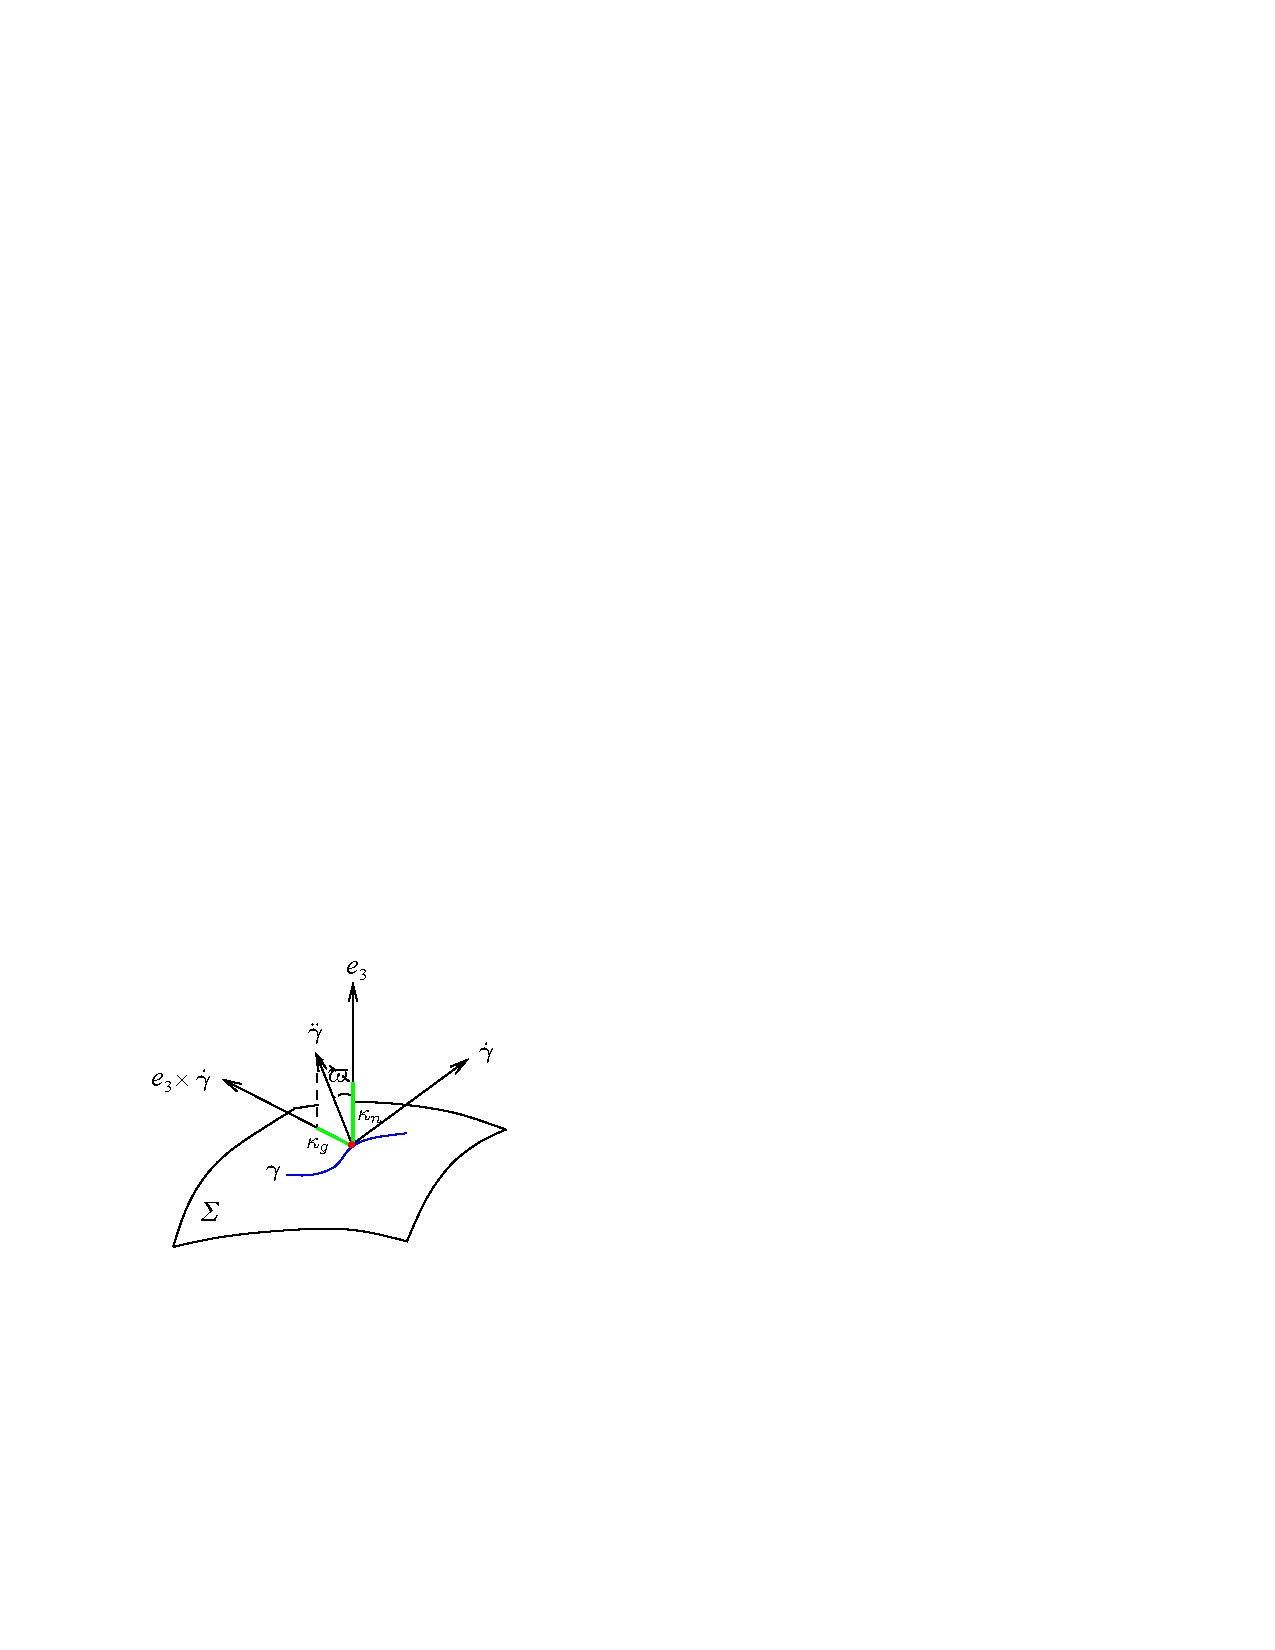
\includegraphics[scale=1]{figures/geodesic.pdf}
    \caption{Geodesic and normal curvatures of a curve on a surface.}
    \label{fig:geodesic curvature}
\end{figure}

A \emph{pseudospherical surface}\index{Pseudospherical surface} is a surface with Gauss curvature $K\equiv -1$. Setting $A=C=-1$ and $B=0$ in the \gls{eds} $\calI$ described in the last \sect. This system is hyperbolic since $B^2-AC=-1<0$, and indeed, the $2$-forms of $\calI$ are spanned by two decomposable forms 
\[\varPsi\pm \varTheta=(\omega_1^3\mp \theta^2)\wedge(\omega_2^3\pm \theta^1).\]
Moreover, we may use the factors of the decomposable forms to express the second fundamental form as 
\[\sfII =\left[\frac12(\omega_1^3+\theta^2)\odot (\omega_2^3+\theta^1)-\frac12(\omega_1^3-\theta^2)\odot(\omega_2^3-\theta^1)\right]\otimes e_3,\]
where $\odot$ is the symmetric tensor product (cf.\ Definitions~\ref{def sym operator} and \ref{def exterior and sym product}). 
This shows that each characteristic curve projects to be an asymptotic line on $\varSigma$.

On an open subset of a pseudospherical surface that is free of umbilic points, we may choose a Darboux framing. This breaks the Cauchy characteristic symmetry of the \gls{eds}, but allows us to see how pseudospherical surfaces are connected to solutions of \gls{sge} (see Examples~\ref{ex sine-gordon} and \ref{ex 7.4.6 Ivey}).

Since we are using Darboux frames,
\[\begin{pmatrix}
    \omega^3_1\\\omega^3_2
\end{pmatrix}=\begin{pmatrix}
    \tan u & 0\\
    0 & -\cot u
\end{pmatrix}\begin{pmatrix}
    \theta^1\\\theta^2
\end{pmatrix},\]
where $u\in (0,\pi/2)$ is half of the angle between the asymptotic lines. We adjoin $u$ as a new variable, and enlarge our \gls{eds} to a Pfaffian system 
\[I=\<\theta^3,\omega^3_1-(\tan u)\theta^1,\omega^3_2+(\cot u)\theta^2\>\]
on $\SE_3\times \bbR$. Then a Darboux framing along a pseudospherical surface corresponds to an integral surface of $\calI=\<I\>_{\mathrm{diff}}$ satisfying the independence condition $\theta^1\wedge\theta^2\neq 0$, and vice versa.

The vanishing of the exterior derivatives modulo $I$ of the last two $1$-forms generating $I$ implies that $\theta^1/\cos u$ and $\theta^2/\sin u$ pull back to be closed $1$-forms on any integral surface. Hence, there exist local coordinates $(t_1,t_2)$ such that 
\[\theta^1=\cos u\dd t_1,\quad \theta^2=\sin u\dd t_2.\]
Moreover, 
\[x\coloneqq (t_1+ t_2)/2,\quad y\coloneqq (t_1-t_2)/2,\] are exactly the arclength parameters along the asymptotic lines. This implies that asymptotic lines form what is called a \emph{Chebyshev net} on the surface: parallel transport of one of the two families of curves along the other preserves it. In other words, opposite edges of the net quadrilaterals have the same length. Thus, one can stretch a flexible ``knitted'' square mesh over this surface. Note also that the asymptotic lines are bisected by the lines of curvature.

Substituting $\dd u=u_x\dd x+u_y\dd y$ into the $2$-forms of the \gls{eds} shows that $\omega_2^1=u_x\dd x-u_y\dd y$ along any integral surface. Then it is easy to see that the structure equation $\dd\omega^1_2=\omega^3_1\wedge\omega^3_2$ (i.e., the Gauss equation) implies that $u$ (or rather $2u$) satisfies \gls{sge}:
\[u_{xy}=\sin u\cos u.\]

Conversely, we may start with a solution of the \gls{sge} and produce a pseudospherical surface by integration. On a fundamental level, note that the First and Second Fundamental Forms of a pseudospherical surface in the asymptotic coordinates $(x,y)$ read 
\[
    \sfI=\begin{pmatrix}
        1 &\cos 2u\\
        \cos 2u & 1
    \end{pmatrix},\quad
    \sfII=\begin{pmatrix}
        0 & \sin 2u\\
        \sin 2u & 0
    \end{pmatrix},
\]
and $2u$ is the angle between the $x$ and $y$-curves. From here it is easy to see that $H=-2\cot(2u)$. \gls{sge} is equivalent to the Gauss-Kodazzi equations on $H$ with $K=-1$, so by the Fundamental Theorem of Surfaces, each solution of \gls{sge} determines a unique immersed surface up to a rigid motion. 

\begin{figure}[tp]
    \centering
    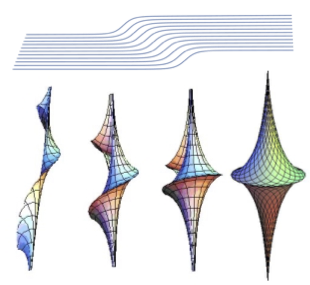
\includegraphics[scale=0.2]{figures/SG1soliton.png}
    \caption{The $1$-soliton solution \eqref{eq SGE 1-soliton} (with lines of constant $y$) of \gls{sge} and the corresponding pseudospherical surfaces for different values of $\lambda^2$. The first three surfaces have the lines of curvature marked on them. The rightmost is the pseudosphere $\lambda=1$ with the asymptotic lines marked on it. Note the asymptotic lines becoming tangent at the edge of the surface.}
    \label{fig: SGE 1-soliton}
\end{figure}

More explicitly, if we let $\frake=(e_1,e_2,e_3)$, then the structure equations $\dd e_i=e_j\omega_i^j$ imply that 
\[\partial_x\frake=\frake \begin{pmatrix}
    0 & u_x & -\sin u\\
    -u_x & 0 & -\cos u\\
    \sin u& \cos u & 0
\end{pmatrix},\quad 
\partial_y\frake=\frake \begin{pmatrix}
    0 & -u_y & -\sin u\\
    u_y & 0 & \cos u\\
    \sin u& -\cos u & 0
\end{pmatrix}.\label{eq 7.21 Ivey}
\]
This is an overdetermined system for the matrix $\frake(x,y)$, and its Frobenius integrability condition is \gls{sge} for $u$. In fact, the above pair of equations is a $UV$-pair for \gls{sge} (see Example~\ref{ex UV pairs}; in fact, this $UV$-pair is equivalent to the one in Example~\ref{ex sine-gordon} under the isomorphism of Lie algebras $\frakso_3\cong\fraksu_2$). So, given a solution to sine-Gordon, we may obtain the framing $\frake$ by solving linear systems of ODEs, and then solve for the surface $\bf{x}(x,y)\in\bbR^3$ by integrating 
\[\bf{x}_x=e_1\cos u-e_2\sin u,\quad \bf{x}_y=e_1\cos u+e_2\sin u.\label{eq 7.22 Ivey}\]
For example, the famous \emph{1-soliton}\index{soliton} solution (also called a \emph{traveling wave} due to its translational invariance, or in the context of the sine-Gordon, a \emph{kink})
\[u=2\arctan(c\exp(\lambda x+\lambda^{-1}y)),\quad c\neq 0, \lambda\neq 0,\label{eq SGE 1-soliton}\]
gives the standard \emph{pseudosphere} when $\lambda^2=1$ and \emph{Dini's surfaces} when $\lambda^2\neq 1$, see Figure~\ref{fig: SGE 1-soliton}.\index{Pseudosphere}\index{Dini's surface} (Note that $c$ can be assumed to be $1$ after a shift and/or flip of one of the axes.)

\begin{figure}[tp]
    \centering 
    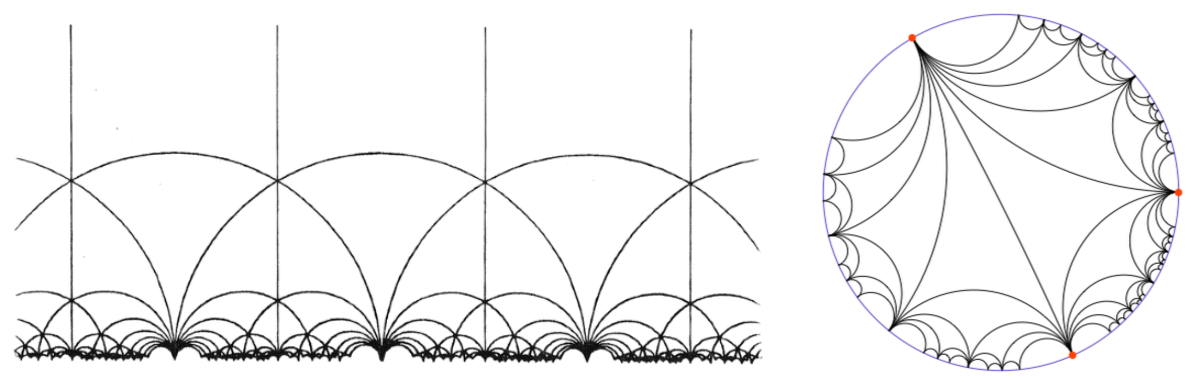
\includegraphics[scale=0.8]{figures/poincare.png}
    \caption{Poincar\'e's hyperbolic half-plane and disk models with some of their geodesics.}
    \label{fig:hyperbolic plane}
\end{figure}

\begin{example}[Hyperbolic plane and disk]\index{Hyperbolic half-plane}\index{Hyperbolic disk}
    The \emph{hyperbolic (half-)plane} is the set $\bbC^+=\{z=x+\i y\in\bbC\mid \Im z>0\}$ with the Riemannian metric 
    \[\sfg=\frac{|\dd z|^2}{(\Im z)^2}=\frac{\dd x^{\otimes 2}+\dd y^{\otimes 2}}{y^2}.\]
    This metric is conformal to the Euclidean one with the conformal factor of $\lambda^2=\frac{1}{y^2}$. The Gauss curvature is found from formula \eqref{eq K in isothermal coords}: $K=\frac12y^2\partial_y^2\ln y=-1$. The geodesics of this surface are semi-circles perpendicular to the $x$-axis and vertical lines.
    
    Another hyperbolic surface of constant negative curvature is the \emph{hyperbolic disk}  $\bbD\coloneqq \{z=x+\i y\in\bbC \mid |z|<1\}$ with the metric 
    \[\sfg=\frac{4|\dd z|^2}{(1-|z|^2)^2}=\frac{4(\dd x^{\otimes 2}+\dd y^{\otimes 2})}{(1-x^2-y^2)^2}.\]
    It is easy to check that $K=-1$ again, and in fact the disk model is isometric to the half-plane one with the isometry given by the biholomorphic \emph{Cayley transform}\index{Cayley transform} 
    \[\bbC^+\to \bbD,\quad z\mapsto \frac{z-\i }{z+\i}.\]
    As a \gls{flt}, it takes circles and lines to circles and lines. As a consequence, the geodesics of the disk model are diametric lines and arcs of circles perpendicular to the bounding circle, see Figure~\ref{fig:hyperbolic plane}.
\end{example}


A Riemannian surface $(\varSigma,\sfg)$ is called \emph{(geodesically) complete} if every geodesic $\gamma(t)$ on it can be extended to all $t\in\bbR$. Equivalently, all vector fields of bounded norm are complete. The following theorem of Hilbert states that pseudospherical surfaces in Euclidean space cannot be complete. This was one of the earliest \emph{global} results in differential geometry. 

\begin{thm}[Hilbert (1901)]\index{Theorem!Hilbert}
    There is no complete immersed surface of constant negative Gauss curvature in $\bbE^3$.
\end{thm}
\begin{proof}
    Hilbert's original proof is a bit lengthy because first one has to establish that the asymptotic lines of any \emph{complete} immersed surface of constant negative curvature can be extended endlessly. Detailed expositions of this proof can be found in \cite[\S5-11]{doCarmo} and \cite[p.~251]{Spivak3}.  We will instead take an advanced shortcut by using the Uniformization Theorem (widely believed to be true since 1882 but first proved by Poincar\'e only in 1907).

    The Uniformization Theorem (in one of its formulations) states that the universal covering of any complete surface $\varSigma$ of constant negative curvature, say $K\equiv -1$, together with the pullback of the metric from $\varSigma$, is isometric to the hyperbolic plane $\bbC^+$.\footnote{This also shows that any non-compact simply connected surface (without boundary) is diffeomorphic to $\bbR^2$.} Now, if we prove that $\bbC^+$ cannot be isometrically immersed into $\bbE^3$, Hilbert's theorem will follow because the universal covering map $\pi:\bbC^+\to \varSigma$ is a local isometry, and so any isometric immersion  $\bf{x}:\varSigma\to \bbE^3$ would allow us to define an isometric immersion $\bf{x}\circ \pi:\bbC^+\to \bbE^3$ (note that we never required the immersions to be injective), leading to a contradiction.

    Now let $2u$ be the solution of \gls{sge} $(2u)_{xy}=\sin 2u$ correspoding to $\bf{x}(\bbC^+)$. Here $(x,y)$ are the asymptotic coordinates on $\bf{x}(\bbC^+)$, not to be confused with the Cartesian coordinates on $\bbC^+$. Since $\bf{x}$ is an immersion, this surface must have linearly independent asymptotic directions at each point, and hence 
    \[0<u(x,y)<\frac{\pi}{2},\quad (x,y)\in \bbC^+.\]
    Now consider a rectangle $R=[a,b]\times [c,d]\subset\bbC^+$ and compute the area of the quadrilateral $\bf{x}(R)$:
    \begin{multline}
        \mathsf{vol}\left[\restr{\bf{x}}{R}\right]=\int_R \sqrt{\det \sfg}\dd x\dd y=\int_R \sin 2 u\dd x\dd y=\int_R (2u)_{xy}\dd x\dd y=\\
        =2(u(b,d)-u(b,c)-u(a,d)+u(a,c))<2\pi.
    \end{multline}
    Since $\bbC^+$ is simply connected and $\bf{x}$ is an immersion, its asymptotic coordinates are globally defined (by stitching together local pieces if necessary), so the rectangle $R$ can be made arbitrarily large. Since the area of the hyperbolic half-plane is infinite, the area of $R$ can become arbitrarily large. This contradicts the above result showing that $\bf{x}(R)$ has bounded area, since $\bf{x}$ is supposed to be an isometry.
\end{proof}


Hence, even if the sine-Gordon solution is defined for all $x$ and $y$, the corresponding surface will become singular. In fact, $\theta^1\wedge\theta^2=\sin 2u \dd x\wedge \dd y$ shows that the surface will be singular whenever $u$ is a multiple of $\pi/2$, i.e., when the asymptotic lines are tangent to each other. This is why the surfaces in Figure~\ref{fig: SGE 1-soliton} have singularities and are made by joining two pseudospherical surfaces along an edge: the values of the $1$-soliton solution always span $(0,\pi)$.

\begin{rem}
    The \gls{sge} has an obvious scaling symmetry given by $x\mapsto \lambda x$, $y\mapsto \lambda^{-1}y$. Hence, each immersion of $\varSigma$ belongs to a one-parameter family of isometric immersions. These deformations of pseudospherical surfaces are called \emph{Lie transformations}. In the next \sect\ we will find a similar one-parameter family of deformations of minimal surfaces (but parametrized by an element of $\U_1$ instead of $\bbR$ because the corresponding system is elliptic).
\end{rem}

\begin{xca}\label{xca 7.4.19 Ivey}
    Note that each of $x+y$ and $x-y$ is constant along one of the two sets of lines of curvature. 
    This observation is useful if we suppose that $\varSigma$ is a pseudospherical surface of revolution (i.e., is spanned by a curve when rotated about a fixed axis). Show that the corresponding sine-Gordon solution can be assumed to be of the form $u=f(x+y)$ (this is easier using the ansatz $u=2\arctan f(x+y)$). Determine all sine-Gordon solutions of this form. 
\end{xca}







\section{Minimal and \texorpdfstring{\gls{cmc}}{CMC} surfaces}

Recall that a minimal surface is an immersed surface $\varSigma<\bbE^3$ with vanishing mean curvature. From Proposition~\ref{prop mean curvature laplace}, an isometric immersion $\bf{x}:\varSigma\to \bbE^3$ is minimal iff it is \emph{harmonic in isothermal coordinates} $(x,y)$:
\[(\partial_x^2+\partial_y^2)\bf{x}=0.\]
In particular, $\bf{x}$ is \emph{conformal}, i.e., it preserves angles between tangent vectors in the $(x,y)$-plane after they're mapped to tangent vectors on $\varSigma$.

Introducing a local isothermal complex coordinate $z\coloneqq x+\i y$ (so that the metric volume form is $\sfv_\sfg=\lambda^2\dd x\wedge\dd y=\lambda^2\frac{\i}{2}\dd z\wedge\dd\wb{z}$), this suggests that there exist $3$ (locally) holomorphic functions of $z$ whose real parts are exactly the Cartesian components of $\bf{x}$. We seek to find this representation now.

Setting $A=C=0$ and $B=1$ in the \gls{eds} for a general linear Weingarten equation shows that the $2$-forms of $\calI$ are spanned 
\[\varTheta=-\dd\theta^3,\quad \varPsi=\omega^3_2\wedge\theta^1-\omega^3_1\wedge\theta^2.\]
This system is elliptic since $B^2-AC=1>0$, so we will have to adjust our method of characteristics to solve it. We will see below that studying the characteristic systems of $\calI$ leads to the classical \emph{Weierstrass representation} for minimal surfaces, which relates them to complex Riemann surfaces.

When we attempt to form the characteristic systems, we find that the decomposability equation 
\[(\varTheta+\lambda\varPsi)^{\wedge 2}=0\]
has constant roots $\lambda=\pm\i$. So, we need to introduce complex-valued differential forms. For example,
\[\varTheta\pm \i \varPsi=(\omega^3_1\mp \i \omega^3_2)\wedge(\theta^1\pm\i \theta^2),\]
and so if we define 
\[\omega\coloneqq \omega^3_1-\i \omega^3_2,\quad \theta\coloneqq \theta^1+\i \theta^2,\]
then the characteristic systems are 
\[\calM=\<\theta^3,\omega,\theta\>,\quad \wb\calM=\<\theta^3,\wb\omega,\wb\theta\>.\]

When we attempt to apply Darboux's method, we find that neither of these systems contains a rank $2$ integrable subsystem. In fact, $\dd\omega\equiv 0\pmod{\omega}$, but $\dd\theta\equiv \wb\omega\wedge\theta^3\pmod{\theta}$. However, this shows that the distribution
\[\Re\<\omega,\wb\omega\>=\<\omega^3_1,\omega^3_2\>\eqqcolon J\]
is a Frobenius system on $\SE_3$. The quotient of $\SE_3$ by the leaves of the distribution dual to $J$ is a $2$-sphere, and the quotient map $\gamma:\SE_3\to \bbS^2$ is given by the unit vector $e_3$. Thus, the restriction of $\gamma$ to an integral surface $M$ of $\calI$ is just the Gauss map of the minimal surface $\varSigma=\pi(M)$, where $\pi:\SE_3\to \bbE^3$ is the bundle projection.

Since $\omega$ descends, via $\gamma$, to a well-defined (up to multiple) form on $\bbS^2$, we can define a complex structure on the sphere for which $\omega$ spans the \emph{$(1,0)$-forms}, i.e., the subbundle of $\T^\ast \bbS^2$ locally spanned by $\dd w$ for a local complex coordinate $w$. We have shown the following fundamental fact.

\begin{cor}
    The Gauss map of a minimal surface $\varSigma$ is holomorphic w.r.t.\ the complex structure on $\varSigma$ defined by $\theta=\theta^1+\i \theta^2$ (as a $(1,0)$-form).
\end{cor}

Now let us fix a standard complex coordinate on $\bbS^2$. We identify $\bbS^2$ with the null quadric $N\subset \CP^2$ defined by $z_1^2+z_2^2+z_3^2=0$ on $\bbC^3$, by mapping $e_3$ to the vector 
\[\mathsf{z}\coloneqq e_1-\i e_2 \quad \in\bbC^3\cong \bbR^3\otimes\bbC.\]
In fact, this vector can be determined from $e_3$ in a unique way, up to a scale, by the requirement that $e_3\times \mathsf{z}=\i \mathsf{z}$. Note that the equation defining $N$ implies that $\lVert\Re \mathsf{z}\rVert^2=\lVert\Im \mathsf{z}\rVert^2=\frac12\lVert \mathsf{z}\rVert^2$.

We then use the stereographic projection 
\[\mathsf{z}=\begin{pmatrix}
    1-w^2\\ \i(1+w^2)\\ 2w
\end{pmatrix},\quad w\in\bbC,\]
to define a complex local coordinate $w$ on $N$ (this actually agrees with the standard stereographic projection $\bbC\to \CP^1\setminus\{\infty\}$ given by $w\mapsto \frac{1}{1+|w|^2}(2w,1-|w|^2)=(x^1+\i x^2,x^3)$, so the resulting complex structure induced by $\omega$ on $\bbS^2$ is the standard one). Computing $\dd\mathsf{z}$ and comparing with $\dd(e_1-\i e_2)=\i(e_1-\i e_2)\omega^1_2+e_3\omega$ shows that $\gamma^\ast\dd w$ is a multiple of $\omega$.

Now suppose $z$ is a complex coordinate on our minimal surface $\varSigma$. Then $\theta=f(z)\dd z$ for a nonvanishing holomorphic function $f$, and $\gamma^\ast w=g(z)$ for some holomorphic function $g$ (we can think of $g(z)$ as another local complex coordinate). Notice that the point $\bf{x}\in \varSigma$ satisfies 
\[\dd \bf{x}=e_1\theta^1+e_2\theta^2=\Re((e_1-\i e_2)(\theta^1+\i \theta^2))=\Re(\mathsf{z}\theta).\]
As a consequence, the First Fundamental Form $\sfI=\<\dd\bf{x},\dd\bf{x}\>$ reads 
\[\sfI=\frac12\lVert\mathsf{z}\rVert^2 |\theta|^2=\frac14 \left(1+|g|^2\right)^2 |f|^2 |\dd z|^2,\quad |\theta|^2\coloneqq \theta\odot\wb\theta.\]
Thus, $z$ is an isothermal coordinate. Similarly, the Second Fundamental Form is 
\[\sfII=-\<\dd e_3,\dd\bf{x}\>e_3=-\Re(\theta \otimes \dd g)e_3.\]
(This is automatically symmetric because $\theta\wedge\dd g\propto \dd z\wedge\dd z=0$.)
In particular, a vector $X$ is an asymptotic direction iff $\theta(X)\dd g(X)$ is imaginary, and principal iff it is real. The Gauss curvature is easy to compute from the conformal factor since the metric is already diagonalized (here we're using informal notation for dividing tensors; the trickiest part is the sign):
\[K=-\frac{|\theta|^2|\dd g|^2}{\left(\frac12\Vert \mathsf{z}\rVert^2 |\theta|^2\right)^2}=-\left(\frac{4|g'|}{(1+|g|^2)^2|f|}\right)^2.\]

Finally, by substituting the expressions for $\mathsf{z}$ and $\theta$ in terms of $z$, we find the \emph{Weierstrass-Enneper representation} of $\varSigma$:
\[\bf{x}=\Re\int \mathsf{z}\theta=\Re\int 
\begin{pmatrix}
    (1-g^2)f\\ \i (1+g^2)f\\ 2gf
\end{pmatrix}\dd z.\label{eq Weiestrass-Enneper}\]
Here, the integral is a contour integral of a holomorphic $1$-form, taken from an arbitrary basepoint to the given point, and is independent of homotopic deformations of the contour with fixed endpoints. Hence, it produces a well-defined function of the endpoint. 

Note that, generally, $g$ is allowed to be a meromorphic function on a domain with nontrivial topology ($\gamma$ takes values in $\bbS^2=\CP^1$, and thus can have poles), which allows $\varSigma$ to have nontrivial topology as well. Moreover, it is obvious from the formulas that the Weierstrass parametrization is regular as long as the poles of $g$ coincide with (and are at most half of the order of) the zeros of $f$.

\begin{cor}[Weiestrass-Enneper representation]\index{Weierstrass-Enneper representation}
    Each nonplanar minimal surface $\varSigma<\bbE^3$ is determined, up to rigid motions, by its Weierstrass data consisting of a meromorphic function $g:\varSigma\to \CP^1$ and a $1$-form $\theta\in\Omega^1(\varSigma;\bbC)$ that is holomorphic w.r.t.\ the complex structure on $\varSigma$ induced by the metric and orientation. Conversely, every such pair $(g,\theta)$ determines a minimal surface via \eqref{eq Weiestrass-Enneper} as long as the poles of $g$ overlap with zeros of $\theta$ so that $g^2\theta$ is holomorphic.
\end{cor}

We can immediately observe that multiplying $f$ (or $\theta$) by a unit complex number produces another valid minimal immersion of the same metric surface.

\begin{defn}[Associate family, conjugate surface]\index{Associate family}\index{Conjugate surface}
    Given a minimal surface $\bf{x}:\varSigma\to \bbE^3$ with Weierstrass-Enneper representation $(g,\theta)$, the one-parameter family of isometric minimal surfaces corresponding to $(g,\rme^{\i t}\theta)$, $t\in (0,2\pi)$, is called the associate family of minimal surfaces.
    
    In particular, the conjugate surface to $\varSigma$ is the surface obtained by multiplying $\theta$ by $\rmi$, or equivalently, by replacing $\Re$ with $\Im$ in \eqref{eq Weiestrass-Enneper}.
\end{defn}

\begin{example}[Catenoid and helicoid]
    The Weierstrass-Enneper representation for the catenoid as parametrized in Example~\ref{ex catenoid} (coordinates $(u,v)$ there are, in fact, isothermal) is 
    \[f(z)=-\i \rme^{-\i z/a},\quad g(z)=\rme^{\i z/a},\quad a>0,\]
    and its conjugate surface is the helicoid (although a slight reparametrization will be necessary to bring to the same form as in Example~\ref{ex helicoid}). This agrees with the standard way of picturing the Riemann surface of $z=\ln w$ as a helicoid. The rest of this $1$-parameter family of surfaces is shown in Figure~\ref{fig:helicoid}.
\end{example}


\begin{xca}
    \begin{enumerate}
        \item Identify the surfaces corresponding to $f=1$ and $g$ being one of $0,z,z^{-1},\i z^{-1}$. The surface with $g(z)=z$ is called the \emph{Enneper surface}\index{Enneper surface} and is the only member of its associate family (in particular, conjugate to itself).
        \item Conclude that the surface obtained by using $(f,g)=(\cos^2\frac{z}{2},\tan\frac{z}{2})$ is regular, and identify it with one of the surfaces in item 1. This shows that the Weierstrass representation of a given minimal surface is not unique.
    \end{enumerate}
\end{xca}

Now let us expand the scope to include \gls{cmc} surfaces. Setting $A=0$, $B=1$, and $C=-2H$, with $H$ a given constant, we get a Weingarten \gls{eds} with $2$-forms 
\[\varTheta=-\dd\theta^3,\quad \varPsi=\omega^3_1\wedge\theta^2+\theta^1\wedge\omega^3_2-2H\theta^1\wedge\theta^2.\]
As with the minimal surface system, the characteristics are complex. The decomposable $2$-forms are 
\[\varTheta+ \i \varPsi=(\omega-H\wb\theta)\wedge\theta\]
and its complex conjugate. This complex coframe, adapted as it is to the characteristics, leads to a simple basis for the \gls{eds} and a simple description of its prolongation. Namely, we adjoin a complex variable $q$ and define the $1$-form 
\[\tau\coloneqq \omega-H\wb\theta-q\theta.\]
The prolongation is the Pfaffian system $\<\theta^3,\tau,\wb\tau\>$ on $\SE_3\times\bbC$. The system $2$-forms are 
\[\dd\tau\equiv -(\dd q+2iq\omega^1_2)\wedge\theta\pmod{\theta^3,\tau,\wb\tau}\]
and its complex conjugate. Note that $q$ parametrizes the components of the traceless part of the Second Fundamental Form. For, $\tau=0$ implies that 
\[\begin{pmatrix}
    \omega^3_1\\\omega^3_2
\end{pmatrix}=\begin{pmatrix}
    H+q_1 & -q_2\\
    -q_2 & H-q_1
\end{pmatrix}\begin{pmatrix}
    \theta^1\\\theta^2
\end{pmatrix},\]
where $q=q_1+\i q_2$. Thus, the zeros of $q$ are the umbilic points of the surface.

\begin{prop}[{{\cite[Prop.~7.4.25]{Ivey}}}]\label{prop 7.4.25 Ivey}
    Let $\varSigma$ be an oriented surface with a Riemannian metric, and let $P$ be its oriented orthonormal frame bundle, with the canonical forms $\eta^1,\eta^2$ and connection form $\eta^1_2$ (see Remark~\ref{rem covariant derivative on surfaces}). Endow $\varSigma$ with the complex structure which it inherits from the metric and orientation. Suppose $q$ is a complex-valued function on $P$ that satisfies 
    \[(\dd q+2\i q\eta^1_2)\wedge(\eta^1+\i \eta^2)=0.\label{eq 7.28 Ivey}\]
    Then 
    \begin{enumerate}
        \item then
        \[Q\coloneqq q(\eta^1+\i \eta^2)^{\otimes 2}\]
        is a well-defined holomorphic quadratic differential on $\varSigma$.
        \item For any constant $H$, $q$ determines a unique local isometric embedding of $\varSigma$ as a \gls{cmc} surface of mean curvature $H$ into $\bbE^3$ up to rigid motions.
        \item An immersed surface is \gls{cmc} iff its Hopf differential (the traceless part of the $\wt{Q}$ defined in \S\ref{sec: theory of surfaces}) is holomorphic.
    \end{enumerate}
\end{prop}
\begin{proof}
    To see that the differential $Q$ is well-defined, let $X$ be the vector field tangent to the fibers of $P$ that is dual to $\eta^1_2$. Then it is easy to check that $\Lie_X Q=0$. To see that it is holomorphic, let $Q=p\dd z^{\otimes 2}$, where $z$ is a local complex coordinate such that $\dd z$ is a multiple of $\eta^1+\i \eta^2$. Then \eqref{eq 7.28 Ivey} implies that $\partial_{\wb z}p=0$.

    Any isometric immersion of $\varSigma$ into $\bbE^3$ will induce an immersion from $P$ to $\SE_3$, and the graph of this map will be an integral $3$-manifold of the Pfaffian system on $P\times \SE_3$ generated by 
    \[\<\theta^3,\theta^1-\eta^1,\theta^2-\eta^2,\omega^1_2-\eta^1_2\>.\]
    To this system we adjoin the form $\tau$ and its conjugate, where $q$ is now given. Our hypothesis about $q$ implies that this enlarged system is Frobenius. Thus, there exists a unique integral $3$-manifold through each point, and any two isometric immersions differ by a rigid motion.
\end{proof}

\begin{cor}[Hopf]\index{Theorem!Hopf}
    Any \gls{cmc} immersion of a sphere $\varSigma=\bbS^2$ (with any metric) is a round sphere, i.e., $K\equiv H^2=\const$.
\end{cor}
\begin{proof}
    It suffices to show that the space of holomorphic quadratic differentials on a sphere is trivial.
    Choose the standard complex structure on the sphere $\CP^1=\bbC\cup \{\infty\}$ given by the complex coordinate $z\in\bbC$. Any \gls{cmc} immersion corresponds to a holomorphic differential $Q=q\dd z^{\otimes 2}$ on $\CP^1$. Then $q$ is a function holomorphic in $\bbC$, and moreover $Q$ needs to be holomrphic at $\infty$, which means that in the local coordinate $w=z^{-1}$, the expression $Q=q(z)w^{-4}\dd w^{\otimes 2}=q(z)z^{4}\dd w^{\otimes 2}$ has to remain regular as $z\to \infty$. Thus $q(z)z^4\to 0$ as $z\to\infty$. But the only holomorphic function in $\bbC$ that has this property is zero, thus $Q=0$ and $K=H^2$.
\end{proof}


\begin{cor}[Bonnet {{\cite[Cor.~7.4.26]{Ivey}}}]
    Any \gls{cmc} surface has a circle's worth of isometric deformations as a \gls{cmc} surface.
\end{cor}
\begin{proof}
    Given $f:\varSigma\to \bbR^3$, let $q$ be the coefficient of the Hopf differential as above and let 
    \[q^t\coloneqq \rme^{\i t}q,\quad t\in(0,2\pi).\label{eq 7.29 Ivey}\]
    Then $q^t$ also satisfies the conditions of Proposition~\ref{prop 7.4.25 Ivey}, and the First Fundamental Form remains unchanged.
\end{proof}

Moreover, if the surface is not totally umbilic, then at most points $q\neq 0$ and the Second Fundamental Form is changed by \eqref{eq 7.29 Ivey}. So, the surface constructed using $q^t$ is, in general, not congruent to the original surface by rigid motions. This is the \gls{cmc} generalization of the isometric deformations of minimal surfaces that we saw above.

\begin{rem}[Bonnet surfaces]
    The above deformations show that there are noncongruent surfaces with the same $K$ and $H$ (in this case, $H$ is the same constant). Bonnet discovered that, besides \gls{cmc} surfaces, there is a finite-dimensional family of surfaces that admit noncongruent isometric deformations preserving $H$. These \emph{Bonnet surfaces} may be characterized by the property that they admit isothermal coordinates (so $q$ is real) and in these coordinates $1/q$ is harmonic, i.e., $(1/q)_{z\wb z}=0$.
\end{rem}










\section{B\"acklund transformations}


Equations which are integrable by the method of Darboux give one example where we can construct integral manifolds of an \gls{eds} by restricting to a submanifold where the system becomes Frobenius. Another example arises when the integrability condition for an overdetermined system of PDEs can be reduced to finding the solution of another PDE. Then any solution of that PDE enables us to construct (using ODE techniques) a solution of the original system.

\begin{example}\label{ex 7.5.1 Ivey}
    For example, the $UV$-pair representation \eqref{eq 7.21 Ivey} of \gls{sge} enables us to construct a solution to the \gls{ma} system for pseudospherical surfaces by integrating a Frobenius system.
\end{example}

When this transformation works in both directions, the two PDEs are said to be related by a \emph{B\"acklund transformation}, which we will define later in the \sect. First, we formalize the relationship between the systems seen in the above examples.

\begin{defn}
    Let $\calI$ be an \gls{eds} on a manifold $M$, let $\pi:B\to M$ be a submersion, and let $\calE$ be an \gls{eds} on $B$. Then $\calE$ is an integrable extension of $\calI$ if there exists a Pfaffian system $J<\T^\ast B$ such that 
    \[\calE=\<J\cup \pi^\ast\calI\>_{\mathrm{alg}}\label{eq 7.31 Ivey}\]
    and $J$ is transverse to the fibers of $\pi$ (i.e. a frame of $J$ pulls back to form coframes on each fiber of $\pi$).  The \emph{rank} of an integrable extension is the rank of $J$, or the dimension of the fibers of $\pi$.
\end{defn}


The condition that $\calE$, as defined by \eqref{eq 7.31 Ivey}, is a differential ideal is equivalent to 
\[\dd\theta\equiv 0\pmod{J,\pi^\ast\calI}\text{ for any }\theta\in\Gamma^\infty(J).\label{eq 7.32 Ivey}\]


\begin{example}[Laplace equation]\index{Equation!Laplace}\label{ex laplace equation backlund}
    The ``baby version'' of a B\"acklund transformation is the Cauchy-Riemann system, which relates pairs of solutions to the $2$-dimensional Laplace equation. Recall from Example~\ref{ex 7.4.6 Ivey} that the Laplace equation $u_{xx}+u_{yy}=0$ is equivalent to the \gls{ma} system on $\rmJ^1(\bbR^2,\bbR)$ generated (differentially) by $\theta=\dd z-p \dd x-q \dd y$ and $\varPsi=\dd p\wedge\dd y-\dd q\wedge \dd x$. We observe that 
    \[\varPsi=\dd (p\dd y-q \dd x)\eqqcolon \dd \phi,\]
    so we can extend the system to $\rmJ^1(\bbR^2,\bbR)\times\bbR$ with a new variable $w$ and let the Pfaffian system $J$ be 
    \[J=\<\dd w-\phi\>=\<\dd w+q\dd x-p\dd y\>.\]
    Clearly $J$ satisfies \eqref{eq 7.32 Ivey} because $\dd (f\phi)\equiv 0\pmod{\<\phi,\varPsi\>}$. Meanwhile, the extended system $\calE$ is a Pfaffian system spanned by $\theta$ and $\phi$, which is equivalent to the following pair of equations on two functions $z=u(x,y)$ and $w=v(x,y)$:
    \[u_x=v_y,\quad u_y=-v_x,\]
    i.e., the Cauchy-Riemann system.\index{Equation!Cauchy-Riemann} Whenever $u,v$ satisfy this system, both $u$ and $v$ must be harmonic. The Cauchy-Riemann system allows one to easily compute $v$ from $u$ (up to constants of integration) using ODE methods. Hence, this system can be seen as a method for generating ``new'' harmonic functions from known ones. Such pairs of harmonic functions are called \emph{conjugate}.\index{Conjugate harmonic function}
\end{example}

If $(B,\calE)$ is an integrable extension of rank $k$ and $N\subset M$ is a $p$-dimensional integral manifold of $\calI$, then \eqref{eq 7.32 Ivey} implies that the pullback of $J$ to $\pi^{-1}(N)$ is Frobenius. In this way, an integral manifold of $\calI$ gives a $k$-parameter family of integral manifolds of $\calE$. In Example~\ref{ex 7.5.1 Ivey}, the $6$-parameter family of surfaces corresponding to a single sine-Gordon solution are congruent under rigid motions of $\bbE^3$.


\begin{example}[\ref{ex 7.5.1 Ivey} continued]
    Let $M=\bbR^5$ and let $\calI$ be the \gls{ma} system for \gls{sge} given in Example~\ref{ex 7.4.6 Ivey}. Let $B=M\times \SE_3$. The equations \eqref{eq 7.21 Ivey} and \eqref{eq 7.22 Ivey} show that a Darboux framing for a pseudospherical surface associated to a sine-Gordon solution $u(x,y)$ is an integral surface for the Pfaffian system 
    \begin{multline}
        J\coloneqq \<\theta^1-\cos u(\dd x+\dd y),\theta^2+\sin u(\dd x-\dd y),\omega^1_2-u_x \dd x+u_y\dd y,\right.\\
        \left. {}\omega^3_1-\sin u(\dd x+\dd y),\omega^3_2+\cos u(\dd x-\dd y)\vphantom{|}\>.
    \end{multline}
    The one can check that $J$ satisfies \eqref{eq 7.32 Ivey}.
\end{example}


\begin{rem}\label{rem 7.5.4 Ivey}
    Suppose $\calI$ is a \gls{eds} on a manifold $M$ with a $2$-form $\varPhi\in\calI^2$ closed. Then, by the Poincar\'e Lemma~\ref{lem poincare classic}, in some contractible neighborhood of any given point in $M$ there exists a differential form $\phi$ such that $\dd\phi=\varPhi$. We may define a rank $1$ integrable extension of $\calI$ by introducing a new coordinate $y$ and letting the Pfaffian system $J$ on $U\times\bbR$ be spanned by $\dd y-\phi$. This is exactly what we did for the Laplace equation in Example~\ref{ex laplace equation backlund}. Because such forms $\varPhi$ are examples of conservations laws for an \gls{eds}, we call this construction an \emph{extension via conservation law}.
\end{rem}


\begin{rem}
    One could trivially produce an integrable extension by choosing $J$ to be Frobenius. Such extensions are called \emph{flat}. More generally, if the derived flag of $J$ terminates in a Frobenius system $K$ of rank $k'$, then $\calE$ defines an intgerable extension when pulled back to any leaf of the foliation dual to $K$. In this case $(B,\calE)$ is called a \emph{$k'$-parameter family} of integrable extensions.
\end{rem}

Parametric families of integrable extensions are frequently encountered in the study of completely integrable PDEs, i.e., \emph{solitonic equations}. 

\begin{example}\label{ex 7.5.6 Ivey}
    We now describe the integrable extensions of the \gls{kdv} equation 
    \[u_t+u_{xxx}+6uu_x=0\label{eq 7.33 Ivey}\]
    (it coincides with \eqref{eq kdv}) after flipping the sign of $u$). Let $M=\bbR^5$ with coordinates $(x,t,u,p,r)$. Let 
    \begin{align}
        \varTheta_1\coloneqq &(\dd u-p\dd x)\wedge\dd t,\\
        \varTheta_2\coloneqq &(\dd p-r\dd x)\wedge\dd t,\\
        \varTheta_3\coloneqq &(\dd r+6u p\dd x)\wedge \dd t-\dd u\wedge\dd x,
    \end{align}
    and let $\calI=\<\varTheta_1,\varTheta_2,\varTheta_3\>_{\mathrm{diff}}$. Then solutions of \eqref{eq 7.33 Ivey} correspond to integral surfaces of $\calI$ satisfying the independence condition $\dd x\wedge\dd t\neq 0$. (Note that $M$ is a quotient of $\rmJ^2(\bbR^2,\bbR)$, and $p,r$ have their classical meanings as $u_x$ and $u_{xx}$ respectively. One could also use the \gls{eds} obtained by pulling back the standard contact system on $\rmJ^3(\bbR^2,\bbR)$ to the hypersurface defined by \eqref{eq 7.33 Ivey}, but the extra variables are not needed here.)

    On $B=M\times\bbR^2$ with fiber coordinates $(\mu,y)$, let $J=\<\dd \mu,\eta\>$, where 
    \[\eta\coloneqq \dd y-(y^2+u-\mu)\dd x+(r+2py+2(u+2\mu)(y^2+u-\mu))\dd t,\]
    and let $\calE=\<J\cup \calI\>_{\mathrm{alg}}$. It is an exercise to verify that $\calE$ is an integrable extension of $\calI$.

    Since $J$ contains a rank $1$ Frobenius system, we have a $1$-parameter family of extensions, with $\mu$ as a parameter. Along an integral surface of $\calE$ that satisfies the independence condition, $y(x,t)$ satisfies 
    \[y_y+y_{xxx}+6(\mu-y^2)y_x=0\label{eq 7.34 Ivey}\]
    for some constant $\mu$. This family of equations may be said to be extensions of \gls{kdv}. When $\mu=0$, it is a version of another well-known PDE, the \emph{modified \gls{kdv} equation}, and the passage from $u$ to $y$ is known as the \emph{Miura transformation}.
    % All integrable extensions of \gls{kdv} have been classified, and each of them corresponds to a finite-dimensional representation of a certain infinite-dimensional Lie algebra, known as the \emph{\gls{kdv} prolongation algebra}. Moreover, this algebra has a $1$-parameter family of finite-dimensional quotients, each of which is isomorphic to a semidirect product of $\fraksl_2(\bbR)$ with $\bbR^5$. Representations of the latter algebra allow us to construct $1$-parameter families of \gls{kdv} extensions, the most well-known of which is the AKNS system \eqref{eq AKNS UV pair}
\end{example}


B\"acklund transformations are a particular form of integrable extension which allows a two-way transformation of solutions of a PDE to solutions of another (or the same) PDE. One of the most well-known is the following transformation, which can produce new solutions of the \gls{sge}.

\begin{example}\label{ex 7.5.9 Ivey}
    Consider the system
    \begin{align}
        u_x-\wb{u}_x=\lambda&\sin(u+\wb{u}),\\
        u_y+\wb{u}_y=\frac{1}{\lambda}&\sin(u-\wb{u}).
    \end{align}
    If $u(x,y),\wb{u}(x,y)$ are smooth functions that satisfy this system for some $\lambda\neq 0$, the differentiating and equating mixed partials implies that $u$ and $\wb{u}$ must be solutions of sine-Gordon $u_{xy}=\sin u\cos u$. Conversely, given a solution $u(x,y)$ of sine-Gordon, we can determine $\wb{u}_x$ and $\wb{u}_y$ from the above, and integrate to get the new solution $\wb{u}(x,y)$ (since we are guaranteed that mixed partials commute). Since this can be done for any $\lambda$, and there will be a constant of integration of the first-order ODE, we get a $2$-parameter family of solutions. For example, the kink solution \eqref{eq SGE 1-soliton} can be produced in this way by starting with $u\equiv 0$. However, the constants of integration amount to translating the solution in the plane, so we can omit them, keeping the translational invariance in mind. Thus, the kink has one parameter $\lambda$. By iterating this procedure, we get a $2$-parameter family of $2$-soliton solutions, a $3$-parameter family of $3$-soliton solutions, and so on. All of them can be obtained by solving simple ODEs and are expressed in terms of trigonometric and exponential functions. For example, the $2$-soliton solution (Figure~\ref{fig:2-soliton}) is 
    \[u=2\arctan \frac{\lambda_1+\lambda_2}{\lambda_1-\lambda_2}\frac{\rme^{\lambda_1x+\lambda_1^{-1}y}-\rme^{\lambda_2 x+\lambda_2^{-1}y}}{1+\rme^{(\lambda_1+\lambda_2)x+(\lambda_1^{-1}+\lambda_2^{-1})y}}.\label{eq sge 2-soliton}\]
    One can also obtain other interesting exact solutions from these formulas. While $\lambda_1$ and $\lambda_2$ are real, we can put $\lambda_1=\rme^{\i t}=-\lambda_2^{-1}$ for $t\in \bbR$, and discover that the formula for the $2$-soliton solution gives another real solution of sine-Gordon, which is periodic in $x-y$ and is called a \emph{breather} (Figure~\ref{fig:breather}).
\end{example}

\begin{figure}[tp]
    \centering
    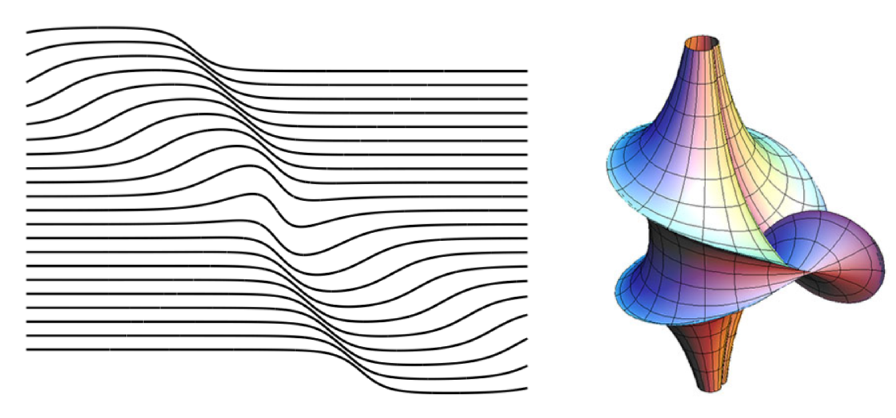
\includegraphics[scale=0.2]{figures/SG2soliton.png}
    \caption{A $2$-soliton solution of \gls{sge} (height profiles at constant $y$ for \eqref{eq sge 2-soliton}) and the corresponding pseudospherical surface.}
    \label{fig:2-soliton}
\end{figure}


\begin{defn}[B\"acklund transformation]
    Let $M_1,M_2$ carry \glspl{eds} $\calI_1$ and $\calI_2$, respectively, and let $B\subset M_1\times M_2$ be a submanifold such that the projections $\pr_i:B\to M_i$, $i=1,2$, give $B$ the structure of a double fiber bundle. Then $(B,\calE)$ defines a B\"acklund transformation between $\calI_1$ and $\calI_2$ if $\calE$ is an \gls{eds} on $B$ that is an integrable extension of both $\calI_1$ and $\calI_2$.
\end{defn}

We will often define B\"acklund transformations by giving a Pfaffian system $J<\T^\ast B$ such that 
\begin{align}
    &\<J\cup \pr_1^\ast \calI_1\>_{\mathrm{alg}}=\<J\cup \pr_2^\ast\calI_2\>_{\mathrm{alg}},\label{eq 7.37a Ivey}\\
    &\calE\coloneqq \<J\cup \pr_1^\ast \calI_1\cup \pr_2^\ast \calI_2\>_{\mathrm{alg}}\text{ is a differential ideal}.\label{eq 7.37b Ivey}
\end{align}
Note that $J$ need not be transverse to the fibers of $\pr_1$ or $\pr_2$.

\begin{example}[\ref{ex 7.5.9 Ivey} continued]
    Let $M_1$ and $M_2$ be two copies of $\rmJ^1(\bbR^2,\bbR)$ where we denote the forms and coordinates on $M_2$ with bars. For $i=1,2$ let the \gls{eds} $\calI_i$ on $M_i$ be a copy of the \gls{ma} system for \gls{sge} from Example~\ref{ex 7.4.6 Ivey}. For any $\lambda\neq 0$, let $B_\lambda<M_1\times M_2$ be defined by $\wb{x}=x$, $\wb{y}=y$ and 
    \begin{align}
        p-\wb{p}&=\lambda\sin(u+\wb{u}),\\
        q+\wb{q}&=\frac{1}{\lambda}\sin(u-\wb{u}).
    \end{align}
    Let $\theta$ be the standard cotact form on $\rmJ^1(\bbR^2,\bbR)$. On $B_\lambda$, let $J=\<\pr_1^\ast\theta,\pr_2^\ast\wb\theta\>$. Then it is easy to check that (\ref{eq 7.37a Ivey}-\ref{eq 7.37b Ivey}) are satisfied.
\end{example}

\begin{figure}[tp]
    \centering
    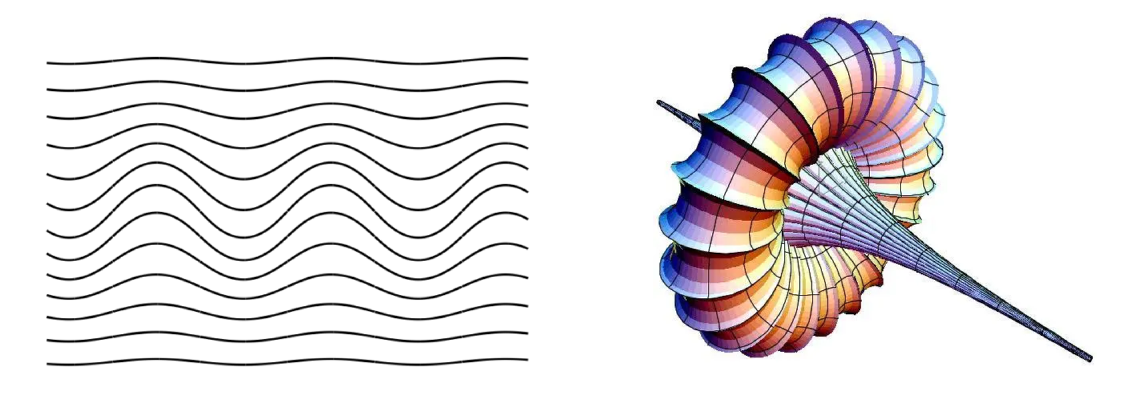
\includegraphics[scale=0.2]{figures/SGbreather.png}
    \caption{A breather wave solution of \gls{sge} (height profiles at constant $x+y$) and the corresponding pseudospherical surface.}
    \label{fig:breather}
\end{figure}


\begin{example}[\ref{ex 7.5.6 Ivey} continued]
    Let $M_1,M_2$ be two copies of $\bbR^5$, each carrying a copy of the \gls{kdv} \gls{eds}. (Again, we use barred coordinates on $M_2$.) Define $B=M_1\times\bbR^2$ as before, and define a submersion $\pr_2:B\to M_2$ by 
    \begin{align}
        \wb{x}&=x,\\
        \wb{y}&=y,\\
        \wb{u}&=2(\mu-y^2)-u,\\
        \wb{p}&=4y(\mu-u-y^2)-p,\\
        \wb{r}&=-4(u+y^2-\mu)(u+3y^2-\mu)-4yp-r.
    \end{align}
    Then $J$, as defined above, gives a B\"acklund transformation between the \gls{kdv} equation and itself. One can check that 
    \[
    \begin{rcases}
        \pr_2^\ast\varTheta_1&\equiv -\pr_1^\ast\varTheta_1\\
        \pr_2^\ast\varTheta_2&\equiv -\pr_1^\ast\varTheta_2-4y\pr_1^\ast\varTheta_1 \\
        \pr_2^\ast\varTheta_3&\equiv -\pr_1^\ast\varTheta_3-4y\pr_1^\ast\varTheta_2-8(u+2y^2-\mu)\pr_1^\ast\varTheta_1
    \end{rcases} \pmod{J}.
    \]
    The presence of an arbitrary parameter in the B\"acklund transformation for \gls{kdv} is central to its complete integrability, both in the sense of inverse scattering and in the Hamiltonian sense.
\end{example}

In many important cases B\"acklund transformations relate two \emph{different} PDEs.

\begin{example}[Wave and Liouville equations]
    Let $M_1\subset \rmJ^2(\bbR^2,\bbR)$ be the submanifold defined by the hyperbolic Liouville equation $z_{xy}=\rme^z$, with the standard contact system $\calI_1$ generated by $\theta_0,\theta_1,\theta_2$ defined in Example~\ref{ex 7.3.6 Ivey}. We use the standard notation $(p,q,r,s,t)$ for the jet coordinates restricted to $M_1$. Then \eqref{eq 7.14 Ivey} implies that $(r-\frac12p^2)_y=0$ and $(t-\frac12q^2)_x=0$ for any solution. Thus, on $B=M_1\times \bbR$ with coordinate $v$ on the second factor, we may define an extension by letting $J=\<\theta_0,\theta_1,\theta_2,\eta\>$, where 
    \[\eta\coloneqq \dd v-(r-\frac12 p^2)\dd x-(t-\frac12 q^2)\dd y.\]
    Because $\dd\eta\equiv 0\pmod{\calI_1}$, $\calE=\<J\cup\calI_1\>_{\mathrm{alg}}$ is an integrable extension of $\calI_1$.

    Furthermore, let $M_2=\rmJ^2(\bbR^2,\bbR)$ with coordinates $(\wb{x},\wb{y},\wb u,\wb p,\wb q)$ and let $\calI_2$ be the standard \gls{ma} system for the wave equation $\wb{u}_{\wb x\wb y}=0$. Define a submersion $\pr_2:B\to M_2$ by 
    \[\wb{x}=x,\quad\wb{y}=y,\quad \wb{u}=v,\quad \wb{p}=r-\frac12 p^2,\quad \wb{q}=t-\frac12 q^2.\]
    Then $\calE$ is an integrable extension of $\calI_2$ (with the role of the transverse Pfaffian system played by $\<\theta_0,\theta_1,\theta_2\>$). Thus, $(B,\calE)$ defines a B\"acklund transformation between Liouville and wave equations.

    Explicitly, the system $\calE$ is equivalent to the two PDEs
    \begin{align}
        u_x+\wb{u}_x&=2\lambda \exp\frac{u-\wb{u}}{2},\\
        u_y-\wb{u}_y&=\frac{1}{\lambda}\exp \frac{u+\wb{u}}{2}.
    \end{align}
    Whenever this system is satisfied, $u$ must be a solution of the Liouville equation, whereas $\wb{u}$ must be a solution of the wave equation. By taking $\wb{u}$, we can recover $u$ up to a constant of integration, thus producing the general solution of the Liouville equation. Letting  $\wb{u}(x,u)=\xi(x)+\eta(y)$, which is the general solution of the wave equation, we separate variables in the above system to find
    \[\exp\left(-\frac{u}{2}\right)=-\exp\left(\frac{\xi-\eta}{2}\right)\left(\lambda\int \rme^{-\xi(x)}\dd x+\frac{1}{2\lambda}\int \rme^{\eta(y)}\dd y\right).\label{eq 9.31 Clellan}\]
    Setting $X(x)\coloneqq -\lambda\int \rme^{-\xi(x)}\dd x$ and $Y(y)\coloneqq -\frac{1}{2\lambda}\int \rme^{\eta(y)}\dd y$, it is easy to solve \eqref{eq 9.31 Clellan} and get the general solution \eqref{eq Liouville general solution}, where $X(x)$ and $Y(y)$ are arbitrary functions of a single variable, with the property that $X'$ and $Y'$ are nonzero and have the same sign.
\end{example}



The B\"acklund transformation for pseudospherical surfaces arises naturally in a classical context, the study of \emph{line congruences} in Euclidean space.

\begin{defn}[Line congruence]\index{Line congruence}
    A line congruence in $\bbE^3$ is an immersed surface in $\Gr_1(\bbE^3)$, i.e., a $2$-parameter family of lines $\ell:U\to \Gr_1(\bbE^3)$, where $U\subset\bbR^2$ and each element of $\Gr_1(\bbE^3)$ (a tangent line to $\bbE^3$) is viewed as a line in $\bbE^3$. It can be expressed (non-uniquely) as 
    \[\ell(\bf{u})=[\bf{x}(\bf{u}),e(\bf{u})],\]
    where $\bf{x}(\bf{u})$ is a point on the line $\ell(\bf{u})$ and $e(\bf{u})\in\bbS^2$ is a unit vector parallel to $\ell(\bf{u})$. If $\bf{x}$ is chosen to be smooth, then the surface $\varSigma=\bf{x}(U)$ is called a \emph{surface of reference} for $\ell$. Any other surface of reference $\wb\varSigma=\wb{\bf{x}}(U)$ for $\ell$ can then be parametrized as 
    \[\wb{x}(\bf{u})=\bf{x}(\bf{u})+\lambda(\bf{u})e(\bf{u}),\quad \lambda\in C^\infty(U).\]

    For a generic line congruence $\ell:U\to \Gr_1(\bbE^3)$ there are two distinguished surfaces of reference, $\varSigma=\bf{x}(U)$, $\wb\varSigma=\wb{\bf{x}}(U)$, called \emph{focal surfaces}, to which each line of the congruence is tangent (we omit the detailed construction). Aside from degeneracies, the lines locally give a $1$-to-$1$ correspondence between points of the focal surfaces.
\end{defn}


\begin{defn}[Pseudospherical line congruence]
    Let $\ell:U\to \Gr_1(\bbR^3)$ be a line congruence with focal surfaces $\varSigma,\wb{\varSigma}$ parametrized as above. The congruence is called pseudospherical if 
    \begin{enumerate}[label=(\alph*)]
        \item The distance $r=\lVert\bar{\bf x}(\bf{u})-\bf{x}(\bf{u})\rVert$ is a constant independent of $\bf{u}$,
        \item The angle $\alpha$ (assumed to be nonzero) between the surface normal vectors $e_3(\bf{u})$, $\wb{e}_3(\bf{u})$ to the surfaces $\varSigma,\wb\varSigma$, respectively, is a constant independent of $\bf{u}$.
    \end{enumerate}
\end{defn}

\begin{thm}[B\"acklund]\index{Theorem!B\"acklund}
    If $\ell$ is a pseudospherical line congruence with focal surfaces $\varSigma,\wb{\varSigma}$, then both of them have constant Gauss curvature $K=-\frac{\sin^2\alpha}{r^2}$, where $r,\alpha$ are as above. 
    
    Conversely, given a surface $\varSigma$ with $K=-\frac{\sin^2\alpha}{r^2}$, a point $\bf{x}_0\in\varSigma$ and a unit non-principal tangent vector $e_0\in \T_{\bf{x}_0}\varSigma$, there exists a unique surface $\wb\varSigma$ such that if $\bar{\bf x}_0$ is the point corresponding to $\bf{x}_0$, then $\bar{\bf{x}}-\bf{x}_0=r e_0$ and the angle between the surface normals of $\varSigma$, $\wb\varSigma$ at $\bf{x}_0$, $\bar{\bf x}_0$, respectively, is $\alpha$.
\end{thm}
\begin{proof}
    \gls{wlog}, we can assume $\lambda=\sin \alpha$, so that $K\equiv -1$. The starting point  of the proof is adapting frames $(\bf{x},\frake)$ and $(\bar{\bf{x}},\wb{\frake})$ along the two surfaces so that $e_1=\wb{e}_1$ is tangent to the line connecting corresponding points $\bf{x}$ and $\bar{\bf x}$. For any fixed $\lambda$, the graph of the B\"acklund transformation is a $6$-dimensional submanifold of $\SE_3\times\SE_3$ defined by 
    \begin{align}
        \bar{\bf x}&= \bf{x}+\lambda e_1,\\
        \bar{e}_1 &= e_1,\\
        \bar{e}_2 &= e_2\cos \alpha+e_3\sin\alpha,\\
        \bar{e}_3&=e_3\cos \alpha-e_2\sin\alpha.
    \end{align} 
    However, we will regard this system as defining a $7$-dimensional submanifold $B<\SE_3\times\SE_3\times\bbR$ with $\lambda$ as the extra coordinate. On $B$, let $J=\<\theta^3,\wb\theta^3,\dd\lambda\>$. Then the exercise below verifies that (\ref{eq 7.37a Ivey}-\ref{eq 7.37b Ivey}) are satisfied, and B\"acklund's Theorem follows from the fact that 
    \[\<\omega^3_1\wedge\omega^3_2+\theta^1\wedge\theta^2,\wb\omega^3_1\wedge\wb\omega^3_2+\wb\theta^1\wedge\wb\theta^2\>\equiv \<\dd\theta^3,\dd\wb\theta^3\>\pmod{J}.\]
\end{proof}



\begin{xca}
    \begin{enumerate}
        \item Differentiate the system of equations in the above proof to obtain the following relations between the pullbacks to $B$ of the canonical forms:
        \begin{align}
            \wb\theta^1&=\theta^1+\dd\lambda,\quad \wb\omega^2_3=\omega^2_3-\dd\alpha,\\
            \begin{pmatrix}
                \wb\theta^2\\\wb\theta^3
            \end{pmatrix}&=
            \begin{pmatrix}
                \cos\alpha & \sin\alpha \\
                -\sin\alpha & \cos\alpha
            \end{pmatrix}\begin{pmatrix}
                \theta^2-\lambda\omega^1_2\\
                \theta^3-\lambda\omega^1_3
            \end{pmatrix},\\
            \begin{pmatrix}
                \wb\omega^1_2\\\wb\omega^1_3
            \end{pmatrix}&=
            \begin{pmatrix}
                \cos\alpha & \sin\alpha \\
                -\sin\alpha & \cos\alpha
            \end{pmatrix}\begin{pmatrix}
                \omega^1_2\\
                \omega^1_3
            \end{pmatrix},
        \end{align}
        Using these, verify (\ref{eq 7.37a Ivey}-\ref{eq 7.37b Ivey}).
        \item Show that \eqref{eq 7.37a Ivey} implies that decomposable $2$-forms in one system are congruent to decomposables for the other modulo the contact forms $\<\theta^3,\wb\theta^3\>$. The asymptotic lines are dual to the factors of these decomposables, therefore the B\"acklund transformation takes asymptotic lines to asymptotic lines.
        \item Show that if two pseudospherical surfaces are related by a B\"acklund transformation, then their corresponding solutions of \gls{sge} are related by a B\"acklund transformation with the same parameter $\lambda$.
        \item Show that B\"acklund transformations are transitive, so the existence of a B\"acklund transformation between two systems is an equivalence relation on \glspl{eds}.
    \end{enumerate}
\end{xca}


As we wrap up our exploration of the geometry of surfaces, we can make some observations about the deep relationship between surfaces and completely integrable systems. As we have seen, many basic problems about surfaces get reduced to integrable systems such as the Liouville equation, \gls{sge}, and the AKNS system. In fact, the \gls{kdv} equation also describes certain classes of surface, and various extensions of these systems appear as well. Aside from geometry of surfaces and dynamical systems, integrable systems appear across all sectors of mathematics: probability and statistics, combinatorics, statistical mechanics, classical analysis, numerical analysis, asymptotic representation theory, algebraic geometry, and so on. While there is no general formal definition of a completely integrable system, all of the following features are considered necessary parts of integrability:
\begin{enumerate}
    \item \emph{A linearizing coordinate transformation}, after which the problem is reduced to linear equations. This property is the most natural extension of the classical notion of integrability (existence of action-angle variables). For example, the Weierstrass representation of minimal surfaces reduced the problem to the linear Cauchy-Riemann system describing holomorphic functions. Similarly, the \gls{kdv} dynamics become linear after being put in terms of the scattering data of the Schr\"odinger equation in which the \gls{kdv} solution acts as the potential. 
    \item \emph{B\"acklund transformations} that allow one to generate solutions of one integrable system using solutions of another.
    \item \emph{A Hamiltonian structure} which describes solutions as Hamiltonian flows on an infinite-dimensional manifold.
    \item \emph{An infinite-dimensional Lie algebra of symmetries}, which generates an infinite number of conserved quantities (analogs of initial data in a Frobenius system).
    \item \emph{Existence of solitonic solutions}, each of which is described by a finite set of parameters related to the conserved quantities. This is another manifestation of the large space of symmetries.
    \item \emph{Well understood function spaces}, such as special functions (elliptic, hypergeometric, Painlev\'e). Even if a nonlinear coordinate transformation is found that reduces the problem to a linear one, the space of solutions to the resulting linear problem needs to be highly legible. A standard criterion for this property is the \emph{Painlev\'e Test}, which is related to the classification of ODEs whose solutions have certain natural analytic properties (such as singularities only of Fuchsian type whose locations are independent of the initial condition), a generalization of the Cauchy-Kovalevskaya Theorem. Solutions to Painlev\'e equations encompass all classical special functions and are currently the broadest well-studied class of special functions related to integrable PDEs.
    \item \emph{Lax pair or zero curvature representations}, which couple the original system with a linear time-dependent operator ($L$ in Example~\ref{ex Lax pairs}) whose dynamics is \emph{isospectral}. The existence of a Lax pair is often conflated with integrability, but it alone does not actually imply the rest of the features listed above.
\end{enumerate} 

For a much more detailed review of the concept of integrable systems, we direct the reader to \cite{deift}. For more on the theory of classical integrable systems, see the books \cite{moser,babelon}.





\section{Gauss-Bonnet and Poincar\'e theorems}\label{sec: gauss-bonnet}

We finish this \chap\ with a classical theorem that is a major early milestone in the history of differential geometry due to being the first \emph{global} result of the theory of surfaces. Moreover, it turns out to relate local geometric data (Gauss curvature) to global topological data, which is independent of the choice of metric, thus becoming a harbinger of the more modern results about topological invariants constructed out of geometric data.


Suppose $\frake=(e_1,e_2)$ and $\wt\frake=(\wt e_1,\wt e_2)$ are two local orthonormal frames on a Riemannian surface $(\varSigma,\sfg)$. They are related by $\wt\frake=\frake\cdot R$ for some function $R:\varSigma\to \SO_2$. We have seen that the \emph{local connection form} $\omega\coloneqq\frake^\ast\omega^2_1$ is intrinsic and can be expressed using an isometric immersion of $\varSigma$ into $\bbE^3$ via 
\[e_2\omega=\dd e_1-\<\dd e_1,e_3\>e_3,\] 
where $e_1,e_2,e_3$ are treated as $\bbR^3$-valued functions on $\varSigma$. (One can also obtain an intrinsic formula for $\omega$ in terms of $\sfg$ but we won't need it in this \chap.) From here, the rotation matrix $R$ induces the following transformation of the connection form:
\[\wt\omega =\wt{\frake}^\ast\omega^2_1=\omega+R^{-1}\dd R.\]
The rotation matrix $R$ is of course uniquely identified with a counter-clockwise rotation through some angle $\theta(m)$ dependent on the point $m\in \varSigma$. In terms of this angle, 
\[\wt\omega =\omega+\dd\theta.\label{eq 169}\]

Now consider a curve $\gamma:[0,1]\to \varSigma$ which lies in a region covered by an orthonormal frame $\frake$. Suppose that $X\in\fX(\varSigma)$ is a vector field whose values $X(t)$ along $\gamma$ have unit length. We define a map $\alpha:[0,1]\to \bbS^1\subset \bbR^2$ by letting $\alpha(t)$ be the image of $X(t)$ under the unique linear map $\im \gamma\to \bbR^2$ which takes $e_1(\gamma(t))$ to $\bf{e}_1=(1,0)$. We then have a continuous map $\phi:[0,1]\to \bbR$ with $\alpha(t)=(\cos\phi(t),\sin\phi(t))$, and any two such maps differ by a multiple of $2\pi$. We will refer to any such $\phi$ as a continuous choice of the angle between $e_1$ and $X$. It is easy to see that $\phi$ is actually smooth if $X$ and $\gamma$ are. 

By choosing another local frame $\wt\frake$ such that $\wt e_1=X$ along $\gamma$ and using \eqref{eq 169}, it is now easy to see that 
\[\nabla_{\dot\gamma}X=0 \Leftrightarrow \omega(\dot\gamma(t))+\dot\phi(t)=\wt\omega(\dot\gamma(t))=\<\nabla_{\dot\gamma}X,\wt e_2\> =0.\]
We say that $X$ is \emph{parallel} along $\gamma$ when this holds. It follows that the connection form $\omega$ describes the rate at which a vector rotates while being parallel transported along $\gamma$. If $X$ is not parallel along $\gamma$, we get a nonzero quantity. In \S\ref{sec: pseudospherical surfaces} we defined the geodesic curvature and noted that it is intrinsic since $\kappa_{\mathrm{g}}=\lVert\nabla_{\dot\gamma}\dot\gamma\rVert$, or 
\[\kappa_{\mathrm{g}}=\<\nabla_{\dot\gamma}\dot\gamma,\bf{N}\>.\label{eq geodesic curvature}\]
In terms of the angle $\phi$ between $e_1$ and $\dot\gamma(t)$, we have 
\[\kappa_{\mathrm{g}}(t)=\omega(\dot\gamma(t))+\dot\phi(t).\]


\begin{prop}
    Let $(\varSigma,\sfg)$ be a compact oriented Riemannian surface, with connected boundary $\partial \varSigma$, diffeomorphic to a subset of $\bbR^2$. Let its Gaussian curvature be $K$ and its canonical area form $\sfv_\sfg$. Let $s$ be the arclength parameter along $\partial \varSigma$ and let $\kappa_{\mathrm{g}}$ be the signed geodesic curvature of $\partial \varSigma$ (on which the direction is induced by orientation). Then 
    \[\int_\varSigma K\sfv_\sfg=-\oint_{\partial \varSigma}\kappa_{\mathrm{g}}\dd s+2\pi.\]
\end{prop}
\begin{proof}
    Because of our assumptions, we may as well assume that $\varSigma\subset \bbR^2$. On it we define a positively oriented orthonormal frame $(e_1,e_2)$ be requiring $e_1$ to be a positive multiple of $\partial_{x^1}$. Let $\gamma:[0,1]\to \partial \varSigma$ be a closed curve, parametrized by arclength $\sigma$, such that $\dot\gamma(\sigma)$ is positively oriented, and let $\phi$ be a continuous choice of the angle between $e_1$ and $\dot\gamma$. Let $\omega$ be the connection form, which in this case can be defined globally. Then, using the Stokes-Cartan Theorem and the above formula for $\kappa_{\mathrm{g}}$,
    \begin{align}
        \int_\varSigma K\sfv_\sfg&=\int_\varSigma K\theta^1\wedge\theta^2=-\int_\varSigma \dd \omega=-\int_{\partial \varSigma}\omega=\\
        &=-\int_0^1 \omega(\dot\gamma(\sigma))\dd \sigma=\\
        &=-\int_0^1\kappa_{\mathrm{g}}(\sigma)\dd\sigma+\int_0^1\dot\phi(\sigma)\dd\sigma=\\
        &=-\int_{\partial \varSigma}\kappa_{\mathrm{g}}\dd s+\phi(1)-\phi(0).
    \end{align}
    To complete the proof, we have to show that $\phi(1)-\phi(0)=2\pi$. This is done essentially by reducing it to the flat case via a continuous deformation of the metric.

    \begin{enumerate}[label=(\arabic*)]
        \item The number $\phi(1)-\phi(0)$ is a multiple of $2\pi$ since $\phi(0),\phi(1)$ are both choices of the abgle for $\dot\gamma(0)=\dot\gamma(1)$.
        \item Let $\delta$ be the standard metric on $\bbR^2$ (the Kronecker tensor). It is easy to check that for each $\lambda\in [0,1]$, the tensor 
        \[\sfg^\lambda\coloneqq \lambda\sfg+(1-\lambda)\delta\]
        is also a Riemannian metric. Let $(e_1^\lambda, e_2^\lambda)$ be a positively oriented local frame which is orthonormal w.r.t.\ $\sfg^\lambda$ and for which $e_1^\lambda$ is a positive multiple of $\partial_{x^1}$; then let $\phi^\lambda$ be a continuous choice of the angle between $e_1^\lambda$ and $\dot\gamma/\lVert\dot\gamma\rVert^\lambda$. The choice $\phi^\lambda$ clearly depends continuously on $\lambda$ (if we make $\phi^\lambda(0)$ vary continuously). Consequently, $\phi^\lambda(1)-\phi^\lambda(0)$ varies continuously with $\lambda$. Since it is always a multiple of $2\pi$, it must be constant.
        \item When $\lambda=0$, we have $e_1^\lambda=\partial_{x^1}$ and $e_2^\lambda=\partial_{x^2}$, and consequently $\phi^0$ is just a choice of the angle between the $x$-axis and $\dot\gamma$. 
    \end{enumerate}
    So $\phi^0(1)-\phi^0(0)$ is the \emph{total curvature} of $\gamma$, which is  $2\pi$ by the \emph{Hopf Umlaufsatz}: indeed, curvature is the rate of rotation of the tangent to the curve in $\bbR^2$, and so the total curvature is the total change of that angle. But it is easy to see that replacing the tangent line with the line passing through two different points $\gamma(s_1),\gamma(s_2)$, $s_1\leq s_2$, on the curve gives a homotopy, where the original angle is the value along the diagonal $s_1=s_2$, and the total change from $(s_1,s_2)=(0,0)$ to $(1,1)$ is independent of the path taken within the triangle $0\leq s_1\leq s_2\leq 1$. On the other hand, if $s_1=0$ if fixed and $s_2$ increases to $1$, the change is obviously $\pi$ assuming $\gamma$ is a simple closed curve, and similarly for the segment from $(0,1)$ to $(1,1)$.
\end{proof}


In the next theorem we consider a generalization of this result for \emph{piecewise smooth} curves. Namely, a \emph{polygon} in $\varSigma$ is a simple closed curve which is a smooth embedding on each interval $[t_i,t_{i+1}]$ of some partition $0=t_0<\cdots<t_{n+1}=1$. Thus, the one-sided derivatives $\dot\gamma(t_i\pm 0)$ exist but may not coincide. It is clear how to define the vertices and the edges of the polygon. At each vertex $\gamma(t_i)$ we also define the \emph{interior angle} $\iota_i$ as the oriented angle from $\dot\gamma(t_i+0)$ to $-\dot\gamma(t_i-0)$ (if they point in the same direction, then one defines the angle to be either $0$ or $2\pi$ based on the orientation of the nearby pairs $(\dot\gamma(t_i+\epsilon),-\dot\gamma(t_i-\epsilon))$ for small $\epsilon>0$).

Having defined the interior angle $\iota_i$, we define the \emph{discontinuity} $\delta_i$ of $\dot\gamma$ at $t_i$ by 
\[\delta_i\coloneqq \pi-\iota_i\in [-\pi,\pi].\]
This describes the oriented angle from $\dot\gamma(t_i-0)$ to $\dot\gamma(t_i+0)$.

\begin{thm}[Gauss-Bonnet formula (1827-1848) {{\cite[Thm.~6.6]{Spivak3}}}]\index{Equation!Gauss-Bonnet}
    In the setting of the preceding theorem, let $\partial M$ be a polygon with vertices $t_1,\ldots,t_n$ and discontinuities $\delta_1,\ldots,\delta_n$. Then 
    \[\int_\varSigma K\sfv_\sfg=-\oint_{\partial \varSigma}\kappa_{\mathrm{g}}\dd s-\sum_{i=1}^n\delta_i+2\pi=-\oint_{\partial \varSigma}\kappa_{\mathrm{g}}\dd s+\sum_{i=1}^n\iota_i+(2-n)\pi.\]
\end{thm}
\begin{proof}
    The proof proceeds much like in the previous theorem, except on each interval $[t_i,t_{i+1}]$ separately, leading to the sum $\sum_{i=1}^{n+1}(\phi_i(t_i)-\phi_i(t_{i-1}))$ instead of the single $\phi(1)-\phi(0)$. This equals $-\sum_{i=1}^n\delta_i+[\phi_{n+1}(1)-\phi_1(0)]$, so it remains only to show that the last term is $2\pi$. This is done in an obvious way by generalizing the Hopf Umlaufsatz by approximating the polygon with a smooth curve.
\end{proof}


\begin{cor}[{{\cite[Cor.~6.7]{Spivak3}}}]\label{cor 6.7 Spivak3}
    If the sides of the polygon in the last theorem are geodesics, then 
    \[\int_\varSigma K\sfv_\sfg=-\sum_{i=1}^n\delta_i+2\pi=\sum_{i=1}^n\iota_i+(2-n)\pi.\]
    In particular, for a geodesic triangle, the total Gauss curvature equals $\iota_1+\iota_2+\iota_3-\pi$.
\end{cor}

We are now ready to compute the total curvature of a \emph{closed surface}, i.e., a compact one with no boundary. We do this under the assumption that the surface has a \emph{triangulation}, i.e., a (finite in this case) collection  $\{\sigma_i\}$ of diffeomorphic images of the standard triangle (\emph{2-simplex}) $\Delta_2\coloneqq \{\bf{x}\in\bbR^3:0\leq x^i\leq 1,\; \sum_{i=1}^3 x^i=1\}$ such that if two of them intersect, then the intersection must be an edge or a vertex. It is a difficult theorem that every smooth surface has a triangulation (and an analogous statement holds for all smooth manifolds of any dimensionality). For a given triangulation of $\varSigma$, which we treat as a ``curved'' polyhedron, we let 
\[(V,E,F)\coloneqq \text{number of (vertices, edges, faces)}.\]
One can prove directly that the quantity $V-E+F$ is independent of the triangulation, but we will do so indirectly in the following main theorem.

\begin{thm}[Gauss-Bonnet-von Dyck (1888)]\index{Theorem!Gauss-Bonnet}\label{thm gauss-bonnet}
    If $(\varSigma,\sfg)$ is a closed (compact with no boundary) oriented Riemannian surface with Gaussian curvature $K$, canonical area form $\sfv_\sfg$, and some triangulation with numbers $(V,E,F)$ defined as above, then 
    \[\int_\varSigma K\sfv_\sfg=2\pi (V-E+F).\]
    In particular, the integer $(V-E+F)$ is not dependent neither on the triangulation nor on the metric, and is thus a topological invariant called the \emph{Euler characteristic} $\chi(\varSigma)$. \index{Euler characteristic!of a closed surface}
\end{thm}
\begin{proof}
    Let the triangulation consist of faces $\sigma_1,\ldots,\sigma_F$. Let $A_j,B_j,C_j$ be the three interior angles of $\sigma_j$. Then by Corollary~\ref{cor 6.7 Spivak3}
    \[\int_\varSigma K\sfv_\sfg=\sum_{j=1}^F \oint_{\partial \sigma_i}\kappa_{\mathrm{g}}\dd s+\sum_{j=1}^F(A_j+B_j+C_j)-\sum_{j=1}^F 3\pi +\sum_{j=1}^F 2\pi.\]
    Now we note the following equalities that lead to the asserted result.
    \begin{enumerate}[label=(\arabic*)]
        \item $\sum_j \oint \kappa_{\mathrm{g}}\dd s=0$, because each edge of the triangulation appears twice with opposite orientations.
        \item $\sum_j (A_j+B_j+C_j)=2\pi V$ since the sum of all interior angles occurring at each vertex is $2\pi$.
        \item $-\sum_j 3\pi=-3F\pi$. On the other hand, any triangulation has $3F=2E$ since $3F$ is the total number of edges of all faces, each edge being counted twice as it belongs to two faces. So, $-\sum_j 3\pi =2\pi (-E)$.
        \item $\sum_j 2\pi=2\pi F$.
    \end{enumerate}
\end{proof}

\begin{xca}
    It turns out that $\chi(\varSigma)$ completely classifies closed oriented surface up to homeomorphism. Show that a surface of genus $g$ has $\chi=2-2g$.
\end{xca}

The most immediate implications of this theorem are the connections between the bounds on the values of $K$ and the topology of $\varSigma$. For example, if $\varSigma$ admits a flat metric, then it must be (homeomorphic to) a torus, and if it admits a metric of everywhere positive curvature, then it must be a sphere. If $K$ is everywhere negative, then an upper bound on its values puts a lower bound on the genus $g>0$.

The following corollary has to do with the degree of the Gauss map. If $M$ and $N$ are both compact $n$-manifolds, then the \emph{(Brouwer) degree} of a map $f:M\to N$ is defined by the formula \index{Degree (Brouwer)}
\[\int_M f^\ast \omega=\deg f\cdot \int_N\omega\]
for any $\omega\in\Omega^n(N)$. For non-compact manifolds, the degree can also be defined for proper maps by requiring that $\omega$ have compact support. For now, we will not prove the surprising fact that $\deg f$ is an integer independent of $\omega$. In the case of $M=N=\bbS^n$, the degree is exactly the corresponding element of the homotopy group $\pi_n(\bbS^n)\cong\bbZ$ (where the generator of the group is given by the identity map).

\begin{cor}[{{\cite[Thm.~6.10]{Spivak3}}}]
    Let $\varSigma\subset\bbE^3$ be an embedded oriented closed surface and let $e_3:\varSigma\to \bbS^2$ be its Gauss map (normal vector). Then 
    \[\deg e_3=\frac12 \chi(\varSigma).\]
\end{cor}
\begin{proof}
    By definition of the degree, $\int_\varSigma e_3^\ast \omega=\deg e_3\cdot\int_{\bbS^2}\omega$ for all $\omega\in\Omega^2(\bbS^2)$. Choosing $\omega=\sfv_{\bbS^2}$ to be the standard are form on $\bbS^2$, this means that by \eqref{eq gauss map pullback}
    \[4\pi \deg e_3=\int_\varSigma e_3^\ast \sfv_{\bbS^2}=\int_\varSigma K \sfv_\sfg.\]
    Together with the Gauss-Bonnet Theorem, this yields the assertion.
\end{proof}

This relation between the degree and the Euler characteristic can also be proven directly, and in fact holds for hypersurfaces in $\bbE^n$ for any $n$. This was an important intermediate result on the way to the higher-dimensional generalization of the Gauss-Bonnet Theorem.

The final classical theorem involves the notion of the index of a vector field. For a vector field $X\in\fX(\varSigma)$ on a surface $\varSigma$, let $m_0\in \varSigma$ be an \emph{isolated zero}, i.e., $X\neq 0$ in a punctured open neighborhood $U\setminus\{m_0\}$ of $m_0$. Choose $U$ so that it is diffeomorphic to a disk. Then the \emph{index $\ind_{m_0}X$ of $X$ at $m_0$} is defined as the winding number of the map $\bbS^1\to \bbS^1$ given by \index{Index!of a vector field}
\[\bbS^1\ni p\mapsto X(i(p))/\lVert X(i(p))\rVert\in\bbS^1,\]
where $i:\bbS^1\to \partial U$ is a diffeomorphism and $\lVert\cdot\rVert$ is an arbitrary metric. It is easy to see that all possible choices of $U, i$, or the metric lead to homotopic maps, so the index is a well-defined invariant of $X$ itself. 

On a closed surface $\varSigma$, we will consider vector fields $X$ that have only isolated zeros. In this case there can only be finitely many zeros $m_1,\ldots,m_r$, and we define the \emph{(total) index} of $X$ as 
\[\ind X\coloneqq \sum_{i=1}^r \ind_{m_i}X.\]
One can prove directly that $\ind X=\chi(\varSigma)$ for any admissible $X$, as was first done by Poincar\'e in 1881. The idea is to first show that the index is independent of the particular vector field $X$, and then to associate to every triangulation a standard vector field as in Figure~\ref{fig poincare-hopf} whose index is manifestly $V-E+F$. Instead of detailing this argument, we will obtain the same result indirectly via the following theorem.

\begin{figure}[tp]
    \centering
    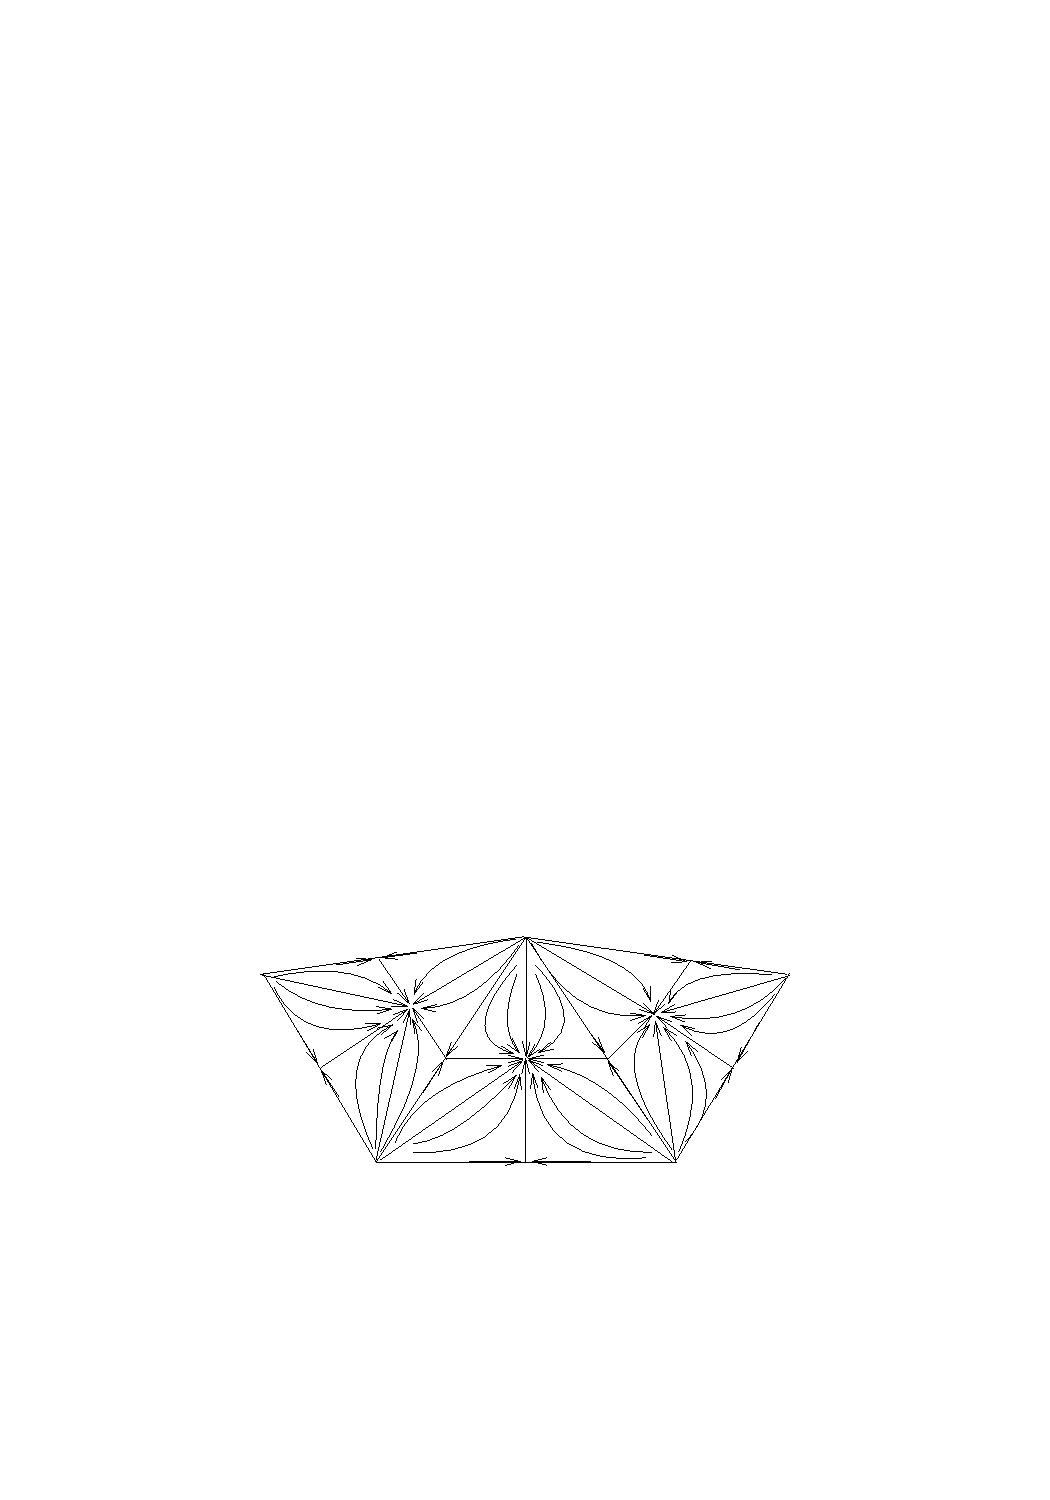
\includegraphics[scale=0.8]{figures/poincare-hopf.pdf}
    \caption{A standard vector field associated to a triangulation in the direct proof of Poincar\'e's Theorem. From \cite{Ivey}. \label{fig poincare-hopf}}
\end{figure}

\begin{thm}[Poincar\'e (1881) {{\cite[Thm.~6.9]{Spivak3}}}]\label{thm poincare-hopf}
    On a closed Riemannian surface $(\varSigma,\sfg)$ with Gaussian curvature $K$ and canonical area form $\sfv_\sfg$, let $X$ be a smooth vector fields with only isolated zeros. Then 
    \[\int_\varSigma K\sfv_\sfg=2\pi \ind X.\]
    In particular, $\ind X$ is independent of $X$ and hence is a topological invariant of $\varSigma$ equal to the Euler characteristic $\chi(\varSigma)$.
\end{thm}
\begin{proof}
    Let $m_1,\ldots,m_r$ be the zeros of $X$, and choose disjoint disks $D_i\subset \varSigma$ containing $m_i$. Each $D_i$ is diffeomorphic to the standard disk $\bbD^2=\{\bf{x}\in\bbR^2\mid \lVert\bf{x}\rVert\leq 1\}$, and we let $D_i(\epsilon)$ denote the set corresponding to $\lVert \bf{x}\rVert\leq \epsilon$. Let 
    \[\varSigma(\epsilon)\coloneqq \varSigma\setminus \left(\bigcup_i \mathring{D}_i(\epsilon)\right).\]
    On $\varSigma(\epsilon)$ there is a positively oriented local frame $(e_1,e_2)$ with $e_1=X/\lVert X\rVert$. Then 
    \[\int_{\varSigma(\epsilon)}K\sfv_\sfg=-\int_{\varSigma(\epsilon)}\dd \omega=-\sum_i \oint_{\partial D_i(\epsilon)} \omega.\]
    Consider one particular $i$. Let $(\wt e_1,\wt e_2)$ be a positively oriented orthonormal frame on $D_i$. On $D_i$ minus a line segment we have a differentiable choice of the angle $\theta$ between $e_1$ and $\wt e_1$, and by \eqref{eq 169},
    \[-\oint_{\partial D_i(\epsilon)}\omega=\oint_{\partial D_i(\epsilon)} \dd\theta-\oint_{\partial D_i(\epsilon)}\wt\omega=\ind_{m_i}X-\oint_{\partial D_i(\epsilon)}\wt\omega,\]
    where $\wt\omega$ also depends on $i$. Therefore, 
    \[-\lim_{\epsilon\to 0}\oint_{\partial D_i(\epsilon)}\omega=\ind_{m_i}X,\]
    which concludes the proof.
\end{proof}

\begin{rem}
    We have thus proven the equivalence of three different ways of computing the Euler characteristic of a closed oriented surface: via a triangulation, via the index of a generic vector field, and via the total Gaussian curvature:
    \[\ind X=\chi(\varSigma)=\int_\varSigma K\sfv_\sfg.\]
    The generalization of the equality $\ind X=\chi(M)$ to closed manifolds $M$ of arbitrary dimensionality was obtained by Hopf in 1921 and is known as the Poincar\'e-Hopf Theorem. \index{Theorem!Poincar\'e-Hopf} Meanwhile, the generalization of the Gauss-Bonnet Theorem to closed oriented manifolds of arbitrary even dimensionality was completed by Chern in 1944 and is known as the Chern-Gauss-Bonnet Theorem. We will prove both of these generalizations as part of our discussion of characteristic classes.
\end{rem}




